% Self-contained arXiv source; figures and references are included below.
\newcommand{\DoNotLoadEpstopdf}{}
\documentclass[11pt]{article}
\usepackage[T1]{fontenc}
\usepackage{lmodern,amsmath,amssymb,amsthm,mathtools}
\usepackage[margin=1in]{geometry}
\usepackage{booktabs,longtable,array,enumitem,xcolor}
\usepackage{tikz,flafter,placeins}
\usetikzlibrary{positioning,arrows.meta,calc}
\usepackage[hidelinks]{hyperref}
\usepackage{xurl}
\setlength{\emergencystretch}{3em}
\raggedbottom
\usepackage{microtype}
\makeatletter
\renewcommand*\l@section{\@dottedtocline{1}{0em}{3.8em}}
\makeatother
\newtheorem{theorem}{Theorem}[section]
\newtheorem{lemma}[theorem]{Lemma}
\newtheorem{proposition}[theorem]{Proposition}
\newtheorem{corollary}[theorem]{Corollary}
\theoremstyle{definition}\newtheorem{definition}[theorem]{Definition}
\theoremstyle{remark}\newtheorem{remark}[theorem]{Remark}
\numberwithin{equation}{section}
\newcommand{\HH}{\mathbb H}
\newcommand{\QQ}{\mathbb Q}
\newcommand{\ZZ}{\mathbb Z}
\newcommand{\R}{\mathbb R}
\newcommand{\OK}{\mathcal O_K}
\newcommand{\Tr}{\operatorname{Tr}}
\newcommand{\N}{\operatorname{N}}
\newcommand{\Dfive}{\mathcal D_5}
\newcommand{\act}{\mathrm{act}}
\newcommand{\up}{\mathrm{up}}
\newcommand{\ph}{\varphi}
\newcommand{\cert}[1]{\nolinkurl{#1}}
\newcommand{\supp}[1]{\textsf{#1}}
\newcommand{\src}[1]{\textnormal{\textsf{[#1]}}}
\newcommand{\ip}[2]{\langle #1,#2\rangle}
\newcommand{\norm}[1]{\lVert #1\rVert}
\title{Dimension bounds for hyperbolic Coxeter polytopes}
\author{Alexander Kolpakov}
\date{28 October 2026}
\begin{document}
\maketitle
\begin{abstract}
We prove that a finite-volume hyperbolic Coxeter polytope has dimension
at most fifty-seven. For compact polytopes we obtain the bound seventeen,
and fifteen when the reflection group is arithmetic. The arguments
combine the local structure of Coxeter diagrams with hyperbolic geometry
and exact finite computations.
\end{abstract}
\section{Introduction}

A hyperbolic Coxeter polytope is a convex polytope in real hyperbolic
space whose dihedral angles are integer submultiples of $\pi$.
Reflection in its facets generates a discrete group for which the
polytope is a fundamental domain. Throughout this paper polytopes
have finitely many facets and finite volume, and hyperbolic space
has curvature $-1$. We prove the following dimension bounds.

\begin{theorem}\label{thm:bounds}
Let $P\subset\HH^n$ be a finite-volume hyperbolic Coxeter polytope.
\begin{enumerate}
\item The dimension satisfies $n\le57$.
\item If $P$ is compact, then $n\le17$.
\item If $P$ is compact and the group generated by its facet
reflections is arithmetic, then $n\le15$.
\end{enumerate}
\end{theorem}

The classical upper bound for the dimension of a finite-volume
hyperbolic Coxeter polytope is $995$~\cite{Prokhorov}. Its proof
belongs to the combinatorial approach based on small faces and
the incidence estimates of~\cite{Khovanskii}. For compact
polytopes the previous upper bound is $29$~\cite{Vin84,Vin85}.
This bound also applies to the compact arithmetic case.
The arguments below refine the restrictions imposed by the local
Coxeter diagrams in these three settings.

Finite-volume arithmetic reflection polytopes exist in dimension
 $21$~\cite{Borcherds}. Thus compactness is essential in the third
statement of Theorem~\ref{thm:bounds}. The arithmetic statement here
concerns precisely the compact case; the first two statements
concern all hyperbolic Coxeter polytopes in their respective classes.

\subsection{The local approach}

The proofs share the description of a polytope by the Lorentz inner
products of its outward facet normals. The facets meeting a finite
vertex give a spherical Coxeter diagram. At an ideal vertex, a
horospherical section decomposes into a product of Euclidean Coxeter
simplices, described by affine diagrams. The classifications of
these diagrams organize the possible configurations into classical
and exceptional families. Inverse Gram matrices and the Lorentz
signature then restrict the ways in which further walls can meet
such configurations.

After these common preliminaries, the finite-volume and compact
arguments use different global comparisons. For the finite-volume
bound we assign nonnegative weights to the corners of two-dimensional
faces. Every triangle receives total weight at least two and every
quadrilateral at least one. If $s(F)$ denotes the number of sides
of a two-face, summing these weights bounds
 \[
 \sum_F\bigl(5-s(F)\bigr).
\]
Spherical and affine vertex diagrams give upper bounds for the
weight at each vertex. Incidence formulas give a conflicting lower
bound in dimension $58$. A separate argument treats all higher
dimensions. Finite and ideal vertices enter this comparison through
different local estimates.

For the compact bound, the comparison is geometric. We choose a
vertex farthest from a fixed interior point and retain the resulting
vector throughout the argument. Projections and inverse Gram
matrices express the restrictions from the components of its
spherical diagram as quadratic-form inequalities. Contributions
from different components are compared using this same vector.
The resulting estimates exclude the remaining diagrams in dimensions
at least $18$.

The arithmetic proof begins with the compact bound already
established. Integrality and positivity at the other real embeddings
restrict the ground field and the possible root norms. These
restrictions exclude the remaining configurations in dimensions
 $16$ and $17$. This is the point at which the arithmetic hypothesis
enters; the preceding compact argument is independent of it.

The finite computations are stated as mathematical problems with
specified domains and exact arithmetic. Their algorithms and the
arguments for termination and completeness accompany the required
outputs. Uniform geometric estimates handle the unbounded ranks
and labels before the remaining finite cases are considered.

\subsection{Organization}

Part~I proves the finite-volume bound in
Theorem~\ref{fv:thm:main}. It develops the corner weights, the finite
and ideal vertex estimates, and the incidence contradiction.
Part~II proves the compact bound in
Theorem~\ref{compact:thm:main} by the farthest-vertex comparison.
Part~III proves the arithmetic bound in
Theorem~\ref{arith:thm:main}, using the independently proved result
of Part~II.

Three corresponding groups of proof appendices supply the detailed
arguments. The first gives the local weight rules, forest and cusp
calculations, and the higher-dimensional finite-volume exclusions.
The second gives the component estimates and the remaining compact
diagram cases. The third gives the field and norm restrictions and
the remaining arithmetic cases. Each part introduces its method
before the case analysis; the appendices complete the proofs of
the three statements in Theorem~\ref{thm:bounds}.

\setcounter{tocdepth}{1}
\tableofcontents

\clearpage
\part{Finite-volume polytopes}\label{part:fv}


\section{The finite-volume bound}
\begin{theorem}\label{fv:thm:main}
Every finite-sided, finite-volume real hyperbolic Coxeter polytope has
dimension at most 57.
\end{theorem}
The theorem belongs to the combinatorial approach to dimension
bounds developed by Vinberg, Prokhorov and Khovanskii: small faces
force local contributions that a high-dimensional vertex cannot
accommodate \cite{Prokhorov,Khovanskii}. The largest presently known
dimension of a finite-volume example is 21; Borcherds constructs an
arithmetic reflection group in that dimension \cite{Borcherds}.
Thus the present bound still leaves a substantial existence gap.

This is a computer-assisted argument. The external ingredients are
the spherical and affine classifications, the bounds for minimal
indefinite diagrams, finite-volume vertex-link geometry, the incidence
formulas, and Nikulin's narrow-facet theorem~\cite{Nikulin,NikulinNarrow}.
The local weight inequalities and extension arguments are proved below.

The main argument excludes dimension 58. Appendices~\ref{fv:app:tail}
and~\ref{fv:app:narrow-tail} treat every higher dimension: first by a finite
set of payment families, and then by an all-rank narrow-facet argument.
We do not infer this tail from the single excluded dimension, or pass
to a facet whose angles have not been proved Coxeter. The marked local
rules and their exact arithmetic certificates are internal parts of
the argument, not additional published assumptions.

For a two-face $F$ with $s(F)$ sides, write
 \[
 \Dfive(P)=\sum_F(5-s(F)).
\]
A simultaneous nonnegative corner rule paying at least 2 on each triangle
and 1 on each quadrilateral gives an upper bound for $\Dfive$. The final
rule has finite-vertex charge at most 377. At an ideal vertex its actual
charge $C_{\act}$ satisfies $\kappa-C_{\act}\ge36$, where $\kappa$ is the
link shape curvature. The global lower bound is
 \[
 \Dfive\ge377v_f+\sum_{v\text{ ideal}}\kappa(v)+4205.
\]
The contradiction is therefore
 \[
 0\ge4205+36v_i>0.
\]
The remainder proves the local and arithmetic interfaces that make this
subtraction valid.

\subsection{The common counting argument}

An angle in this paper is a corner $(v,F)$ of an actual two-face.
A payment is a nonnegative weight $w(v,F)$. Write
 $C(v)=\sum_{F\ni v}w(v,F)$ for its total charge at a vertex.
The elementary local-to-global step is worth stating independently
of the particular rule and of the certificate files.

\begin{lemma}[Payment comparison]\label{fv:lem:payment-comparison}
Suppose every triangular face receives total payment at least 2
and every quadrilateral receives at least 1. Then
 \[
 \Dfive(P)\le\sum_v C(v).
\]
More generally, suppose an incidence argument gives
 \[
 \Dfive(P)\ge Bv_f+\sum_{v\text{ ideal}}\kappa(v)+\Delta,
 \qquad\Delta>0,
\]
while a simultaneous payment rule has $C(v)\le B$ at every finite
vertex and $C(v)\le\kappa(v)-\varepsilon$ at every ideal vertex,
where $\varepsilon\ge0$. These hypotheses are inconsistent.
\end{lemma}
\begin{proof}
A face with $s$ sides needs payment at least $5-s$. This is2
for a triangle and 1 for a quadrilateral. For $s\ge5$ it follows
from nonnegativity. Sum over faces and then over their corners.
Combining the resulting upper bound with the proposed lower bound
gives $0\ge\Delta+\varepsilon v_i>0$.
\end{proof}

% BEGIN ILLUSTRATION_20261026_FV57_CORNERS
\begin{figure}[tbp]
\centering
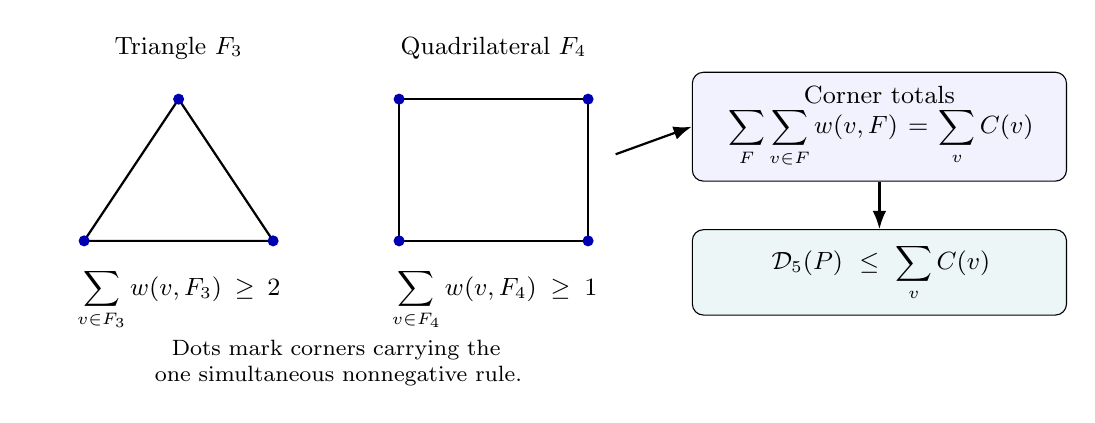
\begin{tikzpicture}[font=\small,>=Latex,
 ledger/.style={draw,rounded corners,fill=blue!5,align=center,
 text width=4.4cm,minimum height=1.05cm,inner sep=5pt}]
 \coordinate (ta) at (.4,1.1);
 \coordinate (tb) at (2.8,1.1);
 \coordinate (tc) at (1.6,2.9);
 \draw[thick] (ta)--(tb)--(tc)--cycle;
 \foreach \v in {ta,tb,tc} {\fill[blue!70!black] (\v) circle (2pt);}
 \node at (1.6,3.55) {Triangle \(F_3\)};
 \node[align=center,text width=3.6cm] at (1.6,.35)
   {\(\displaystyle\sum_{v\in F_3}w(v,F_3)\ge2\)};
 \coordinate (qa) at (4.4,1.1);
 \coordinate (qb) at (6.8,1.1);
 \coordinate (qc) at (6.8,2.9);
 \coordinate (qd) at (4.4,2.9);
 \draw[thick] (qa)--(qb)--(qc)--(qd)--cycle;
 \foreach \v in {qa,qb,qc,qd} {\fill[blue!70!black] (\v) circle (2pt);}
 \node at (5.6,3.55) {Quadrilateral \(F_4\)};
 \node[align=center,text width=3.8cm] at (5.6,.35)
   {\(\displaystyle\sum_{v\in F_4}w(v,F_4)\ge1\)};
 \node[ledger] (sum) at (10.5,2.55)
   {Corner totals\\
    \(\displaystyle\sum_F\sum_{v\in F}w(v,F)=\sum_v C(v)\)};
 \node[ledger,fill=teal!7] (bound) at (10.5,.7)
   {\(\displaystyle\mathcal D_5(P)\le\sum_v C(v)\)};
 \draw[->,thick] (7.15,2.2)--(sum.west);
 \draw[->,thick] (sum)--(bound);
 \node[align=center,text width=7.0cm,font=\footnotesize] at (3.6,-.45)
   {Dots mark corners carrying the one simultaneous nonnegative rule.};
\end{tikzpicture}
\caption{Corner weights in Lemma~\ref{fv:lem:payment-comparison}.
Summing first over faces and then over vertices gives the upper
bound for $\Dfive(P)$.}
\label{fv:fig:ill20261026:fv57:corners}
\end{figure}
% END ILLUSTRATION_20261026_FV57_CORNERS
The geometry enters in choosing a rule that works at every actual
face. The computation enters after that reduction, when the possible
vertex diagrams and their contextual costs have been specified.
The same corner may not be spent twice merely because two local
arguments could have used it: all priorities and compensations must
belong to one simultaneous rule.
Appendix~\ref{fv:app:weights} gives that rule explicitly, as a function
of a marked whole vertex diagram. For the preliminary finite count
we use the same tables with the stated $B_{13}$ endpoint restored
and without the final three rank-15-guarded changes. We call this
preliminary function the preceding rule below.

The proof first separates into finite and ideal vertices. At a finite
vertex we maximize the rule over spherical forests of total rank 58.
At an ideal vertex we bound each affine factor, multiply by its
actual corner-fiber multiplicity, and compare with the curvature of
the product link. These branches reunite in the payment comparison.
The final changes to the rule use whole components: a visible path
inside a larger component does not carry the same contextual bonus.
Figure~\ref{fv:fig:proof-branches} records this division.

\begin{figure}[t]
\centering
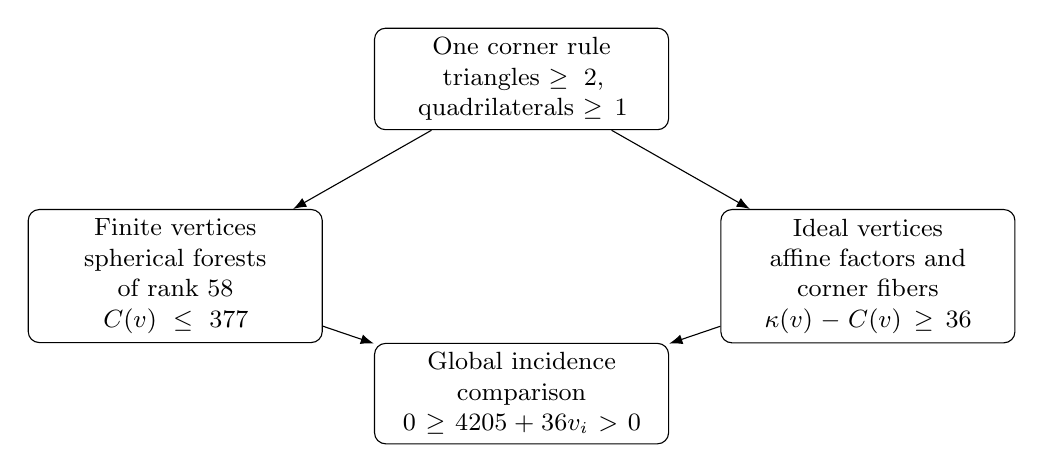
\begin{tikzpicture}[>=Latex,font=\small,
 box/.style={draw,rounded corners,align=center,text width=3.5cm,
 minimum height=1.1cm},node distance=1cm and .65cm]
 \node[box] (local) {One corner rule\\
 triangles $\ge2$, quadrilaterals $\ge1$};
 \node[box,below left=of local] (finite) {Finite vertices\\
 spherical forests of rank 58\\$C(v)\le377$};
 \node[box,below right=of local] (ideal) {Ideal vertices\\
 affine factors and corner fibers\\$\kappa(v)-C(v)\ge36$};
 \node[box,below=2.7cm of local] (global) {Global incidence comparison\\
 $0\ge4205+36v_i>0$};
 \draw[->] (local)--(finite);
 \draw[->] (local)--(ideal);
 \draw[->] (finite)--(global);
 \draw[->] (ideal)--(global);
\end{tikzpicture}
\caption{The common geometric rule is established before the finite
and ideal calculations separate. The strict correction $4205$ comes from
the two extrema of a generic linear function on the polytope.}
\label{fv:fig:proof-branches}
\end{figure}

\section{Corner weights and spherical diagrams}
\label{fv:sec:finite-interface}
We use outward norm-two roots, with diagonal Gram entries2 and
nonpositive off-diagonal entries. At an actual two-face in dimension $n$,
the supporting white roots form a positive-definite rank $n-2$ diagram.
White roots together with one black side give a strictly positive-definite
edge diagram; adjacent corners are positive semidefinite. A finite corner
has an elliptic forest of rank $n$.

These assertions refer to actual faces of the original chamber. We
record two elementary feasibility arguments that will also control
additional supporting roots. Let $p$ be a strict interior timelike
point. A positive-definite principal Gram matrix $B$ has nonpositive
off-diagonal entries and an entrywise nonnegative inverse. If
 $b_i=-(p,e_i)>0$, then
 \[
 q=p+\sum_i(B^{-1}b)_i e_i
\]
is orthogonal to the selected roots and has
 $q^2=p^2-b^TB^{-1}b<0$. It is future pointing and strict against
every other chamber wall. Thus a positive principal set has an
actual finite common point, rather than merely a formal Gram model.

An irreducible affine principal set has a positive kernel vector
 $(u_i)$. Its root combination $\nu=\sum_i u_i e_i$ is null and
nonzero, since $(p,\nu)<0$. It is feasible against every chamber
wall. Its projective point is an ideal vertex: an ideal-sphere point
is extreme in the closed Klein ball and hence in the chamber.
The affine diagram is a whole factor of that cusp, because every
proper principal subdiagram of an irreducible affine diagram is
positive definite. This is also the containment input
of~\cite[Section~1]{FeliksonTumarkin}.

\begin{lemma}[Opposite sides and minimal cores]\label{fv:lem:opposite-cores}
For either opposite pair of sides of an actual quadrilateral, the
supporting whites and that pair form an indefinite principal set.
An inclusion-minimal indefinite subset contains both marked sides.
Its order is at most ten; if all proper principal subsets are
elliptic, its order is at most five.
\end{lemma}
\begin{proof}
A positive set would have an actual common finite point by the
projection argument. A positive-semidefinite singular set would
have a common ideal point by its affine kernel. Opposite closed
sides of a nondegenerate quadrilateral are disjoint, so neither is
possible. Deleting either marked side leaves a subset of an actual
finite edge diagram. Hence both marks lie in every minimal
indefinite subset. The published Lann\'er/quasi-Lann\'er order
bounds now apply; the classification through order ten
is~\cite{Chein}.
\end{proof}

Two such opposite cores cannot be disjoint and orthogonal, since
that would give two negative directions. Their overlap or a joining
path supplies an adjacent-side route. The local theorem must then
restore all the other supporting whites; an argument on the displayed
cores alone would not justify a whole-component payment.

A whole component is a connected component of the full actual corner
diagram, not merely of a displayed core. Presence conditions in a weight
refer only to such whole components. This distinction is essential when
additional supporting whites are restored.

\begin{lemma}[Two ways to seal a component]\label{fv:lem:seals}
Let $G$ be the Gram matrix of an actual indefinite core.
\begin{enumerate}
\item A Gram-kernel vector $z$ of this core gives the actual zero
root relation $\sum_i z_i e_i=0$. Every further wall therefore
satisfies $\sum_i z_i(e,e_i)=0$.
\item Suppose $G$ is nonsingular, an added forest contacts it only
at a position $p$, and $(G^{-1})_{pp}=r>1$. If every connected
component of the added forest contacts $p$, its total rank is at
most $1/(r-1)$.
\end{enumerate}
\end{lemma}
\begin{proof}
The span of an indefinite core contains a timelike vector. The root
combination associated with a Gram-kernel vector is null and
orthogonal to that timelike vector. The perpendicular space is
positive definite, so the combination is zero. This differs from
the nonzero feasible null vector of an affine block.

For the second statement let $B$ be the positive Gram matrix of all
added supporting whites, including indirect tails, and let $u$ be
their contact column at $p$. Schur elimination and the one-negative-
direction condition give $B-r uu^T\succeq0$, whence
 $u^TB^{-1}u\le1/r$.

For a connected square-two finite Coxeter Gram of rank $k$, every
inverse diagonal is at least $k/(k+1)$. This follows by induction:
delete the chosen node, let the remaining component ranks be $k_j$,
and use a contact of magnitude at least one into each component.
Inverse positivity gives Schur cost at least
 $\sum_j k_j/(k_j+1)\ge(k-1)/k$. The resulting inverse diagonal
is at least $1/(2-(k-1)/k)=k/(k+1)$; the rank-one base is $1/2$.
For an added forest of total rank $M$ contacted in each component,
the same bound gives $u^TB^{-1}u\ge M/(M+1)$.
Thus $M/(M+1)\le1/r$, proving $M\le1/(r-1)$.
\end{proof}

The second argument takes all roots of the growing forest at once.
A bound on its immediate neighbors would leave indirect extensions
uncontrolled. For a radical seal, nonpositive contact signs and the
displayed zero relation restrict every further root; the local
short-path alternatives then force either a persistent payment or
orthogonality. An indirect extension has a first contacting root,
so this is the step that turns a core component into a whole one.

At an ideal vertex with affine factor ranks $r_i$, the link is
 $\prod_i\Delta^{r_i}$, with $\sum r_i=n-1$. A marked pair in factor $i$
occurs in $\prod_{j\ne i}(r_j+1)$ actual corner fibers. Hence an affine
factor envelope $(r+1)c(r)$ gives
 \begin{equation}\label{fv:eq:envelope}
 C_{\act}\le C_{\up}=V\sum_i c(r_i),\qquad V=\prod_i(r_i+1).
\end{equation}
The factor-fiber theorem includes nonsimple ideal vertices. Whole affine
factors used locally are established by the positive kernel and actual
corner semidefiniteness, before applying this multiplicity.
Indeed an edge of the product link varies in just one simplex factor.
A fixed pair of its facet labels determines an edge in that factor
and an arbitrary vertex in every other factor. These are precisely
the $V/(r_i+1)$ fibers. The marked pair restores the varying affine
factor; all other factors appear with one node deleted. Summing an
unweighted copy of each affine table would miss this multiplicity.

\subsection{The finite forest algorithm}

For the finite calculation multiply charges by64. Its alphabet is
 \[
 \{A_r:1\le r\le58\}\cup\{B_r:2\le r\le58\}
 \cup\{D_r:4\le r\le58\}
 \cup\{E_6,E_7,E_8,F_4,H_3,H_4,I_2^*\}.
\]
The rank-two symbol $I_2^*$ represents all remaining $I_2(m)$,
$m\ge5$, in the cost calculation. The local all-label theorem
gives their common relevant charge and interactions; this notation
is not a finite cutoff on $m$ or an identification of their metrics.
An admissible formal forest has multiplicities $m_T\ge0$ with
 $\sum_T\operatorname{rank}(T)m_T=58$. Actual finite vertices are
among these forests. The calculation needs no converse realization
theorem.

The ordinary cost consists of a component table $b(T)$ and a
symmetric interaction table $j(T,U)$; context bonuses are separate.
In particular $j(T,T)$ concerns two distinct copies of $T$.
The cost is
 \begin{align}\label{fv:eq:forest-cost}
 C_{64}(m)&=\sum_T b(T)m_T+\sum_T j(T,T)\binom{m_T}{2}\notag\\
 &\quad+\sum_{T<U}j(T,U)m_Tm_U+\Psi(m).
\end{align}
The tables and the context function belong to the simultaneous
local rule. Their identification with actual corner charges is a
geometric obligation, separate from maximizing this expression.
Appendix~\ref{fv:app:routing} supplies the actual-face coverage and
triangle arguments.
Appendix~\ref{fv:app:finite-contexts} specifies the complete context
function and the finite refinement used in this calculation.

Fix all context-sensitive counts before the residual calculation.
After this split the residual alphabet $\mathcal U$ has positive
integer ranks $r(T)$ and additive integer weights $w(T)$, with no
remaining pair interaction. For a residual rank $R\le58$ define
 \begin{equation}\label{fv:eq:forest-dp}
 V(0)=0,\qquad
 V(s)=\max_{\substack{T\in\mathcal U, r(T)\le s\\
                         s-r(T)\text{ reachable}}}
       \{V(s-r(T))+w(T)\}\quad(1\le s\le R).
\end{equation}
An empty maximum is an unreachable state, not an ordinary integer.
Evaluate in increasing rank, recording a last item for each finite
maximum.

\begin{proposition}[Residual certificate]\label{fv:prop:dp-certificate}
The algorithm~\eqref{fv:eq:forest-dp} terminates and computes the exact
maximum over residual multisets. A saved table certifies the same
claim if it has base value zero, dominates every allowed last-item
transition, and has a tight last-item witness at every positive rank
carrying a finite stored value. At positive ranks, a state is
unreachable exactly when it has no reachable last-item predecessor;
rank zero is the reachable base.
\end{proposition}
\begin{proof}
There are at most 59 ranks and finitely many transitions at each
rank. Every predecessor has smaller rank. By induction, removing
one component from any nonempty multiset bounds its weight by one
of the candidates in~\eqref{fv:eq:forest-dp}. Conversely, append the
chosen component to an attaining predecessor multiset. This proves
both inequalities and reachability. The same induction applies to
a saved table using all its transition inequalities and tight
witnesses at every stored finite value. Positive item ranks make
each tight predecessor smaller, so strong rank induction rules out
spurious finite entries. Following witnesses reaches zero after at
most 58 steps.
Checking only an attaining path would not bound omitted multisets.
\end{proof}

In the actual context split, fixed representative counts have
 $\sum_{r=9}^{17}rc_r\le58$, with a separate $A_{12}/D_{12}$
split, fixed $A_{17}$, and $0\le k_5\le
\lfloor(58-\sum rc_r)/5\rfloor$. The residual ranks are
 $1,2,3,4,6,7,8$ and 17 through 58. Expand every class that can exceed
377 into all actual-type fibers. Within each fiber fix the complete
 $A_1,A_2$ counts. For the only remaining presence guard, split into
no $A_3$ or reserve one $A_3$ and allow further copies without
repeating its $D_{14}$ bonus. The two exceptional increasing families
are bounded separately, rather than omitted from the context cover.
All count ranges are bounded by rank 58. These facts prove termination
of the full context algorithm; the geometric domination theorem
establishes that its cover includes every actual forest.

\begin{proposition}[Computed finite interface]\label{fv:prop:oldcount}
The preceding simultaneous rule in ambient 58 pays every triangle at
least2 and every quadrilateral at least 1. Every actual rank 58 finite
forest has charge at most 377 except precisely the following eight formal
forests: one $B_{13}$ or $D_{13}$ together with any multiset of three
 $A_{15}$ or $D_{15}$ components. Each of those eight has charge378.
All ideal weights admit the envelope of Section~\ref{fv:sec:ideal}.
\end{proposition}
\begin{proof}[Certificate and completeness argument]
The frozen coupled count starts from the complete 3298 fixed-vector/rank 5
cover, retaining fixed $A_{17}$ separately from residual $D_{17}$ and
separating the $A/B_{12}$ and $D_{12}$ interaction types. Simultaneous actual
base and cross-cost domination covers exceptional finite types and the
arbitrary-label rank-two family. Its two potentially increasing context
families are bounded separately:759 rows for the $A_1/D_5$ upgrade, and
539 rows for the $A_2/A_4$ guarded family, with all 14 costly rows refined
through 77 actual assignments. Both bounds are strictly below377.

The complementary complete 39 costly classes have748 fixed actual-type
fibers. All actual $A_1,A_2$ multiplicities are fixed explicitly. The
remaining $A_3$ presence guard is split into no $A_3$ and one reserved $A_3$;
the latter may contain more $A_3$ without multiplying the presence bonus.
All other context guards are fixed, and residual pair interactions vanish.
The 1549 fresh residual tables certify every allowed last-item inequality,
unreachable rank and attaining predecessor. Induction on an item's removal
therefore proves their upper bounds for arbitrary residual multisets.
Reconstructing every winning forest verifies its full contextual cost.
All 38 other classes are at most 377; the residual-zero rank 13-plus-three15
class gives exactly the eight listed forests. Their charge is $78+3(100)$.

The local inequalities establishing that these costs give valid corner
weights are proved in Appendix~\ref{fv:app:routing}.
\end{proof}

A separate frozen $B_{13}$ endpoint theorem removes pair $(0,12)$, with no
new coupon. Its complete selected domain has no affected image, but that
absence alone is insufficient: two older affine-$B_{13}$ singleton routes
really consumed the endpoint unit. Their whole cores instead give distinct
already-unit $A_1/D_{12}$ short-leaf contributions. The other endpoint-like
pair $(1,12)$ needed by the current $D_{12}$ theorem is retained. Thus the
four $B_{13}$ forests in Proposition~\ref{fv:prop:oldcount} drop to 377.

\section{The dimension-specific final local rule}
\begin{theorem}[Three-rank 15 transfer]\label{fv:thm:local}
In ambient dimension 58, make these changes to the simultaneous rule:
\begin{enumerate}
\item In a whole finite $D_{13}$, give pairs $(0,11),(0,12)$ weight $1/2$
instead of 1 only if its actual corner has three distinct whole unmarked
 $A_{15}$ or $D_{15}$ components.
\item Add $1/2$ to whole $D_{28}$ pair $(0,12)$ only if its corner has two
such whole unmarked rank 15 components.
\item Add $1/2$ between an endpoint of whole $A_{12}$ and the long endpoint
of whole $D_{16}$ under the same two-component presence guard.
\end{enumerate}
All ideal weights and other finite weights remain. Every triangle still
pays at least 2 and every quadrilateral at least 1.
\end{theorem}
Witnesses are not counted with multiplicity. The negative guard uses
 $13+3\cdot15=58$ ranks, so the corner has exactly those four components.
The two positive guards similarly force exactly $D_{28}+2\cdot15$ or
 $A_{12}+D_{16}+2\cdot15$. The theorem is not asserted in larger ambient
dimensions.

\subsection{A general inverse bound for attached forests}
\begin{lemma}\label{fv:lem:inverse}
For a connected positive-definite Coxeter Gram matrix $B$ of rank $k$,
with diagonal2 and every nonzero native magnitude at least 1,
$(B^{-1})_{ii}\ge k/(k+1)$ for every $i$. If a finite forest of total
rank $M$ has a nonnegative contact vector $u$ with at least one unit contact
in every component, then $u^tB^{-1}u\ge M/(M+1)$.
\end{lemma}
\begin{proof}
Inverse matrices of these positive-definite symmetric $Z$-matrices are
entrywise nonnegative. Delete the chosen root; let the remaining connected
components have ranks $k_j$. Every component has a contact with the root.
By induction and inverse positivity its contribution to the root's Schur
projection is at least $k_j/(k_j+1)$. Since
 \[
 \sum_j\frac{k_j}{k_j+1}\ge\frac{\sum_jk_j}{1+\sum_jk_j}
 =\frac{k-1}{k},
\]
Schur complementation gives
 $(B^{-1})_{ii}\ge(2-(k-1)/k)^{-1}=k/(k+1)$.
The rank-one base is $1/2$. Larger native magnitudes or multiple contacts
only increase the lower bound. Apply it in every contacted component of
a forest and use the same sum inequality to prove the second assertion.
\end{proof}

\subsection{Complete selected cases and arbitrary additional whites}
The fresh complete target domain contains801 patterns,862$D_{13}$ maps,
33 affected contexts and 76 affected pair maps. The physical cores have
norm-two roots; full Lorentz, white and all four edge signatures and actual
corner classifications are reconstructed exactly. The native-domain
completeness is inherited from the universal reduction, rather than
claimed from these records alone.

There are five proper completions. Their missing fork leaf is genuinely
new: old corner roots outside the displayed $A_{12}$ are orthogonal to it.
Its forced unit contact has inverse projection square6,12,30 or102,
exceeding2. Additional same-end contacts cannot lower the bound. Mixed-end
contacts give an independently paid short path. Thus these completions
are impossible.

Four radical cores, numbered1985,2378,2575,2581, seal the entire displayed
core. Indeed the whole selected $D_{13}$ forbids contacts on its nodes;
every remaining contact position has a nonzero radical coefficient. A new
white must pair to zero with the radical. Nonempty contacts therefore
meet both signs and give a retained adjacent-black shortcut of length at
most8. Otherwise all contacts vanish and the unmarked $A_4$ is whole.
It cannot coexist with the three rank 15 witnesses.

Twelve contexts similarly have a small displayed block with no permitted
new contact of projection at most 2. It is whole: any indirect extension
would have a first new root contacting it. The rank-capacity guard again
excludes it.

In the final twelve contexts the old small factor $K$ has rank $s=1,2,3$.
Its unique permitted contact position $p$ has core-inverse square
 $r=4/3,3/2,2$, respectively. The native gap excludes magnitudes greater
than 1; positive-end inverse bounds exclude two same-end contacts.
Four cases also permit an opposite contact position $q$, with
 $J_{pp}=J_{qq}=4/3$ and $J_{pq}=-4/3$. Two new roots using $p,q$ have residual
squares $2/3$, so their full product is at most $-4/3+2/3=-2/3$. Their
forced native bond supplies the retained short path. Thus, without that
escape, all new whites in a growing $K$ component contact the old core
only at $p$; some may be orthogonal to it.

Let $Y$ contain all new whites in this whole component, including every
indirect tail, and let $M$ be its rank. Every component of $Y$ contacts $K$.
With contact vector $u$, the full Lorentz condition gives the positive
semidefinite residual Schur matrix
 \[
 G_Y-r uu^t\succeq0,
 \qquad u^tG_Y^{-1}u\le1/r.
\]
Lemma~\ref{fv:lem:inverse} implies $rM/(M+1)\le1$, hence
 $M\le3,2,1$ respectively. In all cases the whole $K$ component has rank
at most 4, contradicting the guard. This controls arbitrary supporting
whites, not just immediate neighboring roots.

\subsection{The universal affine-D12 consumer}
The old opposite-fork-leaf affine-$D_{12}$ theorem genuinely used the
newly lowered whole finite $D_{13}$ unit. It must be repaired separately.
Number its affine factor $F$ of order 13 with spine0 through 8, short leaves
9,10 at 0 and 11,12 at 8. Choose ideal marks $a=9,b=11$ and opposite black
roots $c,d$. Let $Z$ be the elliptic spectator forest, orthogonal to $F$,
and $x,y$ the nonnegative contacts of $c,d$ with $Z$.

An adjacent-black bond or a shared spectator neighbor is an independently
paid short path. Otherwise $x,y$ have disjoint supports. The complete
all-label end-profile reduction gives each end cost at most 8; a
nonextreme end has cost at most 4. The exact Schur identity is
 \[
 \frac{\det S}{h^2k^2}
 =1-\frac{g_c+g_d}{12}
  +\frac1{12}(x/h-y/k)^tG_Z^{-1}(x/h-y/k).
\]
Its determinant vanishes at the actual four-black star.

If an end is nonextreme, equality forces costs8 and 4 and $x=y=0$.
A quiet root attached to the selected old leaf gives the retained whole
 $A_1/D_{12}$ short-leaf unit. If it attaches to the mate, it gives whole
 $D_{13}$. Without the new guard its unit is unchanged. With the guard,
$Z$ consists of exactly three orthogonal whole rank 15 factors.
The three nonextreme equality profiles give, at a distinct corner,
respectively a retained $A_1/D_{12}$ unit, an independent whole affine
 $B_{13}$ priority, or a second guarded $D_{13}$ half. These exhaust24
physical cases. The current $B_{13}$ endpoint repair uses its $D_{12}$
cross unit, not a newly financed $D_{13}$ route; there is no circularity.

When both ends are extreme,$h=k=1/2$, and the determinant becomes
 \begin{equation}\label{fv:eq:energyone}
 (x-y)^tG_Z^{-1}(x-y)=1.
\end{equation}
The old two-nonempty-support theorem gives retained short paths or small
sealed alternatives. The changed $D_{13}$ output belongs to the arbitrary
one-sided branch, say $y=0$. The quiet corner excludes $c$ and retains $Z$
orthogonally. If its $D_{13}$ guard holds,$Z$ is exactly three whole
 $A_{15}/D_{15}$ factors.

\begin{lemma}\label{fv:lem:rank 15}
Under the strict edge conditions and disjoint-support hypothesis,
energy1 on three whole $A_{15}/D_{15}$ factors forces a single unit contact
at the long endpoint of one $D_{15}$, by one black root. The other two
factors have zero contact with both black roots.
\end{lemma}
\begin{proof}
For $A_{15}$ the inverse diagonal entries below2 occur only at nodes
0,1,13,14. They are $15/16$, $7/4$, $7/4$, and $15/16$, respectively.
Two native contacts give energy
at least 2 and violate strict edge positivity. The complete profiles are
simple contacts at these four nodes or doubled contacts at 0,14. The next
native squared magnitude $(3+\sqrt5)/2$ is already excluded.
For $D_{15}$ only its long endpoint has inverse diagonal below2, equal
to 1, and only its simple contact fits.

Every allowed nonzero component energy is at least $15/16$; no $A_{15}$
profile has energy1. The finite exact inverse table also checks every
disjoint two-sided profile difference: all are at least $15/16$ and none
is1. Equal-node contacts are forbidden by disjoint support. Two active
components would have total at least $15/8>1$. Equation~\eqref{fv:eq:energyone}
therefore forces precisely the stated $D_{15}$ contact.
\end{proof}

The two inactive components are orthogonal to the entire star and the
active component. They remain whole, without indirect bridges. If $c$
attaches to selected $a$, the opposite corner is whole $A_{12}$ at an
endpoint and whole $D_{16}$ at its long endpoint. If it attaches to $a$'s
mate, that corner is whole $D_{28}$ at $(0,12)$. Both physical30-root
models have signature $(28,1,1)$, positive white rank 26, positive edge
rank 27 and semidefinite corners. In either case the new half, guarded by
the two inactive rank 15 factors, supplements the quiet $D_{13}$ half
at a different actual corner. This proves the required total1.

\subsection{Chosen-output and triangle retention}
The previous selected and nonselected routes must retain their chosen
positive contributions, including every later replacement route. The
low66 contexts have order bound at most 12. The 74 protected and 9 adaptive
paths have length9, whereas the changed $D_{13}$ role has distance11.
The current finite6/7/8 and cycle/tree routes terminate at short paths,
protected leaves, small whole factors or unchanged ideal contributions.

The older affine-$D_{11}$ repairs use $D_{13}(1,11)/(1,12)$ units, retained
here. The current center/leaf theorem uses $D_{13}(0,10)$, at its fork
center. The coupled order 11 unmixed boundary gives $D_{11+r}$ marks
 $(r,n-2)/(r,n-1)$ of distance9; for $r=2$ these are disjoint $D_{13}$ roles.
The other current finite and contextual outputs are similarly retained.
The new producer reconstructs all 216 literal configurations,564 later
corners,24$D_{14}$ variants,332 positive $D_{12}$ outputs and the newer
sealed families. These finite checks support the named interfaces;
universal completeness remains the written routing theorem. The genuine
unstored affine-$D_{12}$ exception was repaired above.

For triangles use the complete actual-face theorem, not three pairs in
one diagram. Lemma~\ref{fv:lem:current-affine-triangle-exclusions} first
excludes the three reduced small affine patterns. Low cores give two
distinct corner paths of length at most 5.
The 1025 high-core triples give paths of length at most 7 or one of four
protected $E_8$ alternatives, with finite marked length6 or7 or whole
exceptional affine order at most 9. Current finite6 deletions retain all
three exceptional length6 alternatives through their nearby whole leaf;
the length7 alternative and other persistent-feature outputs survive.
The present distance11 reduction changes none of these chosen payments.
Ideal contributions are unchanged. This completes
Theorem~\ref{fv:thm:local}.

\section{The new complete finite maximum}
\begin{proposition}\label{fv:prop:finite}
Every actual finite rank 58 forest under the final simultaneous rule has
charge at most 377. The exact formal maximum is377.
\end{proposition}
\begin{proof}
The $B_{13}$ theorem lowers four forests in Proposition~\ref{fv:prop:oldcount}
from 378 to 377. The new $D_{13}$ guard lowers the other four by1. Every
other forest was already at most 377, except that the two new positive
coupon families must be checked.

Rank capacity makes those families exact. They have respectively
 \[
 170+2(100)+\tfrac12=370.5,
 \qquad66+108.5+2(100)+1=375.5.
\]
The second total counts both $A_{12}$ endpoint coupons. The previous
 $A_{12}/D_{16}$ cross cost is zero. Each family has three possible
multisets of two $A_{15}/D_{15}$ factors, so all six actual forests are
covered. No additional context witness can fit. Outside them the change
is pointwise nonincreasing. Thus the bound377 holds everywhere, and the
eight changed forests attain it formally. A geometric realization of an
attainer is neither required nor asserted.
\end{proof}

\section{Positive ideal surplus}\label{fv:sec:ideal}
For affine ranks $r_i$ summing to 57 set
 \[
 \begin{gathered}
 H(t)=\prod_i(1+t+\cdots+t^{r_i})=\sum_{j=0}^{57}h_jt^j,
 \qquad V=\prod_i(r_i+1),\\
 G=\sum_jh_j\min(j,57-j),\qquad\kappa=\frac{5G-57V}{2}.
 \end{gathered}
\]
The geometric all-family envelope is unchanged by every final finite
transfer. Its complete numerical table is
 \[
 c(r)=r/2\quad(1\le r\le8),\qquad
 c(r)=\frac{5r+56}{r+1}\quad(24\le r\le57),
\]
together with the following entries:
\begin{center}\small
\begin{tabular}{c|rrrrrrrr}
$r$&9&10&11&12&13&14&15&16\\\hline
$c(r)$&$71/16$&$53/11$&$31/6$&$11/2$&$40/7$&$367/60$&$411/64$&$227/34$
\end{tabular}
\medskip
\begin{tabular}{c|rrrrrrr}
$r$&17&18&19&20&21&22&23\\\hline
$c(r)$&$119/18$&$128/19$&$137/20$&$146/21$&$155/22$&$163/23$&$85/12$
\end{tabular}
\end{center}
The finite arithmetic below assumes the proved factor-charge envelope
\eqref{fv:eq:envelope}; polynomial evaluation does not establish its
geometric meaning.

\subsection{The terminal-domain algorithm}

Let $\mathcal P(n,\ell)$ be the list of nondecreasing partitions of
 $n$ with parts at least $\ell$. Generate it by
 \[
 \mathcal P(0,\ell)=\{()\},\qquad
 \mathcal P(n,\ell)=\bigcup_{q=\ell}^{n}
       \{(q,p):p\in\mathcal P(n-q,q)\}\quad(n>0).
\]
The union is empty if $\ell>n$. The terminal cusp domain is
 \begin{equation}\label{fv:eq:terminal-domain}
 \mathcal T_{57}=\bigcup_{\ell=0}^{7}
       \{(\ell,p):p\in\mathcal P(57-\ell,8)\},
\end{equation}
where a zero part is omitted. For each profile compute its polynomial
by repeated convolution: start with $h^{(0)}_0=1$, and when adjoining
rank $r$ set
 \[
 h^{(k+1)}_j=\sum_{a=0}^{r}h^{(k)}_{j-a},
\]
with out-of-range entries zero. Then compute $V,G,\kappa$ from their
displayed definitions and set $m=\kappa/V-\sum_i c(r_i)$.

\begin{proposition}[Complete terminal calculation]\label{fv:prop:terminal}
The partition and convolution algorithms terminate, list every
profile in~\eqref{fv:eq:terminal-domain} exactly once, and compute its
margin by exact rational arithmetic. Their recorded complete output
is2552 profiles, with
 \[
 \min_{\mathcal T_{57}}m=\frac{87}{10240}>0,
 \qquad\min_{\mathcal T_{57}}Vm=36.
\]
\end{proposition}
\begin{proof}[Algorithm correctness and computed output]
Every recursive call lowers $n$ by a positive integer, and every
loop is finite. The unique first part of a sorted partition and its
unique tail prove completeness and absence of duplicates by induction
on $n$. Its exceptional part below8, if present, determines the
outer branch $\ell$ uniquely. Polynomial convolution is exactly
multiplication by $1+t+\cdots+t^r$, so induction on the factors
proves every coefficient. Degrees never exceed57. All remaining
operations are finite integer or rational sums and products.

The stated cardinality and minima are the computed proposition:
the complete saved certificate records every rank tuple and
coefficient list, and the independent endpoint checker reconstructs
the domain and every convolution before comparing them. It evaluates
all 2552 margins, rather than checking only degree, symmetry or a
sample of rows. The two minima are separate assertions and need
not have the same attaining profile. The implementation and records
are identified in the reproducibility section.
\end{proof}

\begin{lemma}[Concentrating two simplex ranks]\label{fv:lem:concentration}
Let $1\le a\le b$ be integers, and let $U_r$ be uniform on
 $\{0,\ldots,r\}$. With independent summands,
$U_{a-1}+U_{b+1}$ dominates $U_a+U_b$ in convex order.
Adding any common independent summand preserves this order.
\end{lemma}
\begin{proof}
Both sums have mean $(a+b)/2$ and are symmetric about that mean.
For an integer threshold $t$, let $\Delta_t$ be the difference
of their expectations of $(X-t)_+$. Equal means allow us to use
 $(t-X)_+$ instead, and symmetry gives
 $\Delta_t=\Delta_{a+b-t}$. It suffices to take
 $0\le t\le(a+b)/2$. Put $D=(a+1)(b+1)$ and $D'=a(b+2)$.
For $0\le t\le a$, direct summation of the increasing side of
the two convolution triangles gives
 \[
 \Delta_t=\binom{t+2}{3}\left(\frac1{D'}-\frac1D\right)\ge0,
 \qquad D-D'=b-a+1>0.
\]
For $a\le t\le(a+b)/2\le b$, summing over the first uniform
instead gives
 \[
 \Delta_t=
 \frac{t(a+b-t)-(a-1)(a+2b+2)/3}{2(b+1)(b+2)}.
\]
The numerator is increasing up to $(a+b)/2$. At $t=a$ it is
 $(a+2)(b-a+1)/3>0$. Outside the common support the difference
is zero; between integer thresholds it is linear. Thus all
stop-loss differences are nonnegative. On the integer support the
values of a convex function are an affine function plus a
nonnegative sum of these stop-loss functions, proving convex order. Conditioning
on a common independent summand proves the last assertion.
\end{proof}

\begin{lemma}[Positive low8 reduction]\label{fv:lem:low8}
Every actual ideal vertex has $\kappa-C_{\act}\ge36$.
\end{lemma}
\begin{proof}
For $1\le a\le b\le7$, replacing $(a,b)$ by $(a-1,b+1)$ preserves
normalized envelope cost, since all these ranks stay at most eight.
Lemma~\ref{fv:lem:concentration}, including its independent-summand
assertion, gives the required convex order. Since
 \[
 \frac GV=\frac{57-\mathbb E|2S-57|}{2},
\]
the transfer does not increase normalized curvature or normalized
margin. Its product decreases from $(a+1)(b+1)$ to $a(b+2)$. Iteration
terminates at ranks at least 8 and at most one positive rank below8.
Indeed the integer potential $\sum_i r_i^2$ increases by
 $2(b-a+1)\ge2$ at every step and is bounded above by $57^2$.
Its initial value is at least 57, so at most 1596 steps occur.
Rank zero is omitted. No transfer passes through the changed rank 9
envelope. The stopping domain is exactly~\eqref{fv:eq:terminal-domain}.

Proposition~\ref{fv:prop:terminal} gives positive normalized terminal
margin and absolute envelope surplus at least 36. If the original and terminal quantities
are $(V,m)$ and $(V',m')$, then $V\ge V'$ and $m\ge m'>0$. Thus
 $Vm\ge V'm'\ge36$. This multiplication uses positivity. Finally
\eqref{fv:eq:envelope} transfers the same lower bound to actual cusp charge.
\end{proof}

\section{Shape curvature and the contradiction}
\begin{lemma}\label{fv:lem:shape}
For a proposed ambient 58 polytope,
\[
 \Dfive\ge377v_f+\sum_{v\text{ ideal}}\kappa(v)+4205.
\]
\end{lemma}
\begin{proof}
Choose a generic linear function on the bounded Klein closure of
the polytope. Let $E_v$ be the number of edges of its simple vertex
figure and $E_v^0$ the number not cut by the induced level section.
If $I$ counts all polygon vertices with multiplicity, the published
incidence identities give $I=\sum_vE_v$ and
 $2f_2=\sum_vE_v^0$ \cite[Theorem9]{Khovanskii}. Hence
 $\Dfive=\sum_v(5E_v^0/2-E_v)$.

Orient each vertex figure by its induced generic linear function.
Assign an uncut edge below the section to its upper endpoint and
one above the section to its lower endpoint. A vertex of index $j$
receives $j$ or $57-j$ contributions, at least their minimum.
The index distribution is its $h$-vector
\cite[Theorems2 and 6]{Khovanskii}, so $E_v^0\ge G_v$.
At the distinct global minimum and maximum the whole
vertex figure is uncut, and symmetry gives
 \[
 E_v-G_v=\sum_{j>57/2}h_j(2j-57)\ge\sum_{j=29}^{57}(2j-57)=841.
\]
Every coefficient of a simplex or product-of-simplices $h$-polynomial is
at least 1. Adding the two extrema and multiplying by $5/2$ gives4205,
counted once. For a finite vertex $h_j=1$, so
 \[
 G_0=\sum_{j=0}^{57}\min(j,57-j)=812,
 \qquad\frac{5G_0-57\cdot58}{2}=377.
\]
The remaining ideal terms are precisely $\kappa$.
\end{proof}

For faces with at least five sides,$5-s(F)\le0$. The nonnegative local
rule and Proposition~\ref{fv:prop:finite} therefore give
 \[
 \Dfive\le377v_f+\sum C_{\act}.
\]
Subtract Lemma~\ref{fv:lem:shape} and use Lemma~\ref{fv:lem:low8}:
\[
 0\ge4205+\sum(\kappa-C_{\act})\ge4205+36v_i>0.
\]
This also excludes the all-finite case. Thus dimension 58 is impossible.
Appendices~\ref{fv:app:tail} and~\ref{fv:app:narrow-tail} exclude all
dimensions at least59. This proves Theorem~\ref{fv:thm:main}.


\clearpage
\part{Compact polytopes}\label{part:compact}




\section{The theorem and the organization of its proof}
\label{compact:sec:organization}
Our main result is the following dimension bound.
\begin{theorem}[Dimension bound]
\label{compact:thm:main}
Every compact real hyperbolic Coxeter polytope has dimension at most \(17\).
\end{theorem}
Here compact means that every vertex is finite.

The central object is one vector \(x\), obtained from an original
farthest vertex \(p\). Energies of orthogonal components of its incident
diagram can be added because they are projections of this same vector.
Pressures arising from different auxiliary points cannot in general
be optimized separately and then added. Instead, we combine them in
one reference vector and retain its complete squared norm.

The case split occurs at the finite irreducible components of the
diagram at \(p\). Small components pay uniform energy debits.
A large \(A\)-component is handled in its zero-sum chain coordinates.
A large \(B\)- or \(D\)-component has a long common prefix; its terminal
nodes then require separate analysis. Section~\ref{compact:sec:forests} records a
fresh complete cover at dimension \(18\), and the separate
higher-dimensional cover. A \emph{cover} always means necessary
possibilities, not realized examples. Section~\ref{compact:sec:b18} explains the
whole-\(B_{18}\) terminal partition. Sections~\ref{compact:sec:d18-setup}--%
\ref{compact:sec:composition} give the whole-\(D_{18}\) closure.

The final composition has two parts. We exclude every dimension
at least \(19\) by its actual-rank forest cover and local consumers.
At dimension \(18\), the complete cover leaves only a whole
 \(D_{18}\) diagram at the same selected farthest vertex.

\section{Farthest vertices and projections}
\label{compact:sec:geometry}
Use the hyperboloid model with Lorentz signature \((-+\cdots+)\).
Every wall has an outward unit spacelike normal \(n\), and the polytope
is given by \(\ip{r}{n}\leq0\). Distinct actual wall normals have
nonpositive products. Fix a strict interior point \(z\), choose an
actual vertex \(p\) farthest from \(z\), and write
 \begin{equation}
\label{compact:eq:original}
 z=E(p-x),\qquad E=-\ip{z}{p}>0,\qquad
 x\in p^\perp,\qquad \norm{x}^{2}=1-E^{-2}<1.
\end{equation}
The space \(p^\perp\) is Euclidean. The incident normals at \(p\) form
a positive definite spherical diagram; compact acute simplicity
implies that there are exactly \(n\) of them in dimension \(n\).
We retain these original normals and this original choice of
 \(p,z,x,E\) throughout an energy argument.

The function \(r\mapsto-\ip{z}{r}\) takes its maximum on a compact
hyperbolic polytope at a vertex. Its restriction to a unit speed
geodesic has positive second derivative equal to the function itself,
so a maximum on a segment occurs at an endpoint; successively
passing to proper faces proves the assertion. Consequently
 \begin{equation}
\label{compact:eq:allpoint}
 -\ip{z}{r}\leq E\quad\text{for every actual point }r\in P.
\end{equation}
At an adjacent vertex \(q\), write \(z=E_q(q-y)\).
Equation~\eqref{compact:eq:allpoint} gives a comparison factor \(E/E_q\),
not a claim that \(q\) is farthest.

\subsection{Positive inverse matrices and feasible projections}
\begin{lemma}[Inverse positivity]
\label{compact:lem:inverse}
If a positive definite symmetric matrix \(B\) has nonpositive
off-diagonal entries, then \(B^{-1}\) is entrywise nonnegative.
\end{lemma}
\begin{proof}
Choose \(s\) greater than the largest eigenvalue of \(B\) and all its
diagonal entries. Then \(M=sI-B\) is entrywise nonnegative and has
spectral radius \(s-\lambda_{\min}(B)<s\). Thus
 \(B^{-1}=s^{-1}\sum_{k\geq0}(M/s)^k\) is entrywise nonnegative.
\end{proof}
\begin{lemma}[An actual positive projection]
\label{compact:lem:projection}
Let \(n_j\), \(j\in J\), be actual wall normals with positive
definite Gram matrix \(B_J\), and let \(z\) be strict interior.
Put
 \[
 q_0=z-\sum_{i,j\in J}(B_J^{-1})_{ij}\ip{z}{n_j}n_i.
\]
Then \(q_0\) is future timelike, orthogonal to all selected walls,
and has negative product with every unselected actual wall.
Its normalization is a point of the original polytope.
\end{lemma}
\begin{proof}
The added coefficients are nonnegative by Lemma~\ref{compact:lem:inverse}.
For an unselected wall every added product is nonpositive and the
original product is negative; the selected products vanish.
Moreover
 \[
 q_0^2=z^2-
   (\ip{z}{n_i})_{i\in J}^{T}B_J^{-1}
   (\ip{z}{n_i})_{i\in J}<0.
\]
Since \(\ip{z}{q_0}=q_0^2<0\), it has future orientation.
All original wall inequalities survive normalization.
If fewer than \(n\) walls are selected this is a point on a face,
not an asserted full-dimensional vertex.
\end{proof}
The same sign check applies to positive combinations of actual
normals below: selected products are calculated explicitly; every
unknown original wall has nonpositive product with every summand.
A nonzero feasible future null vector would give a point of the
ideal boundary of \(P\), contradicting compactness. A positive
affine Coxeter kernel on actual walls is an obstruction after its
future sign and all remaining wall products have been checked.

\begin{lemma}[Future-point pressure]
\label{compact:lem:pointpressure}
Suppose \(U\in p^\perp\), \(\xi=A p-U\) is future timelike
with \(\xi^2=-k<0\),
and its normalization is feasible against every actual wall.
Then the same original vector satisfies
 \[
 \ip{x}{U}\geq A-\sqrt{k}.
\]
At a different actual vertex \(q\), use the decomposition
 \(\xi=Aq-U\) with \(U\in q^\perp\). With all-point comparison
factor \(\kappa\), the corresponding inequality is
 \(\ip{y}{U}\geq A-\kappa\sqrt{k}\).
\end{lemma}
\begin{proof}
The spatial hypothesis gives \(A=-\ip{p}{\xi}>0\).
Apply \eqref{compact:eq:allpoint} to \(\xi/\sqrt{k}\):
\(-\ip{z}{\xi/\sqrt{k}}=E(A-\ip{x}{U})/\sqrt{k}\leq E\).
The modified comparison is the identical calculation.
\end{proof}
If \(U\ne0\), its support lies in actual orthogonal components
and \(\norm{U}^2=A^2-k\); Cauchy therefore also gives
 \begin{equation}\label{compact:eq:pointenergy}
 \norm{x_{\operatorname{supp}U}}^2
 \geq\frac{A-\sqrt{k}}{A+\sqrt{k}}.
\end{equation}
Normalize a future vector, not a spacelike correction.
For a cap \(c=A p-v\), clear a positive definite old block \(J\):
\[
 w=\sum_{i,j\in J}(B_J^{-1})_{ij}\beta_j n_i,\quad
 \beta_j=-\ip{c}{n_j}\geq0,\quad
 \eta=c+w,\quad \delta=\eta^2=1-\beta^TB_J^{-1}\beta.
\]
If \(\delta<0\), \(\eta\) is the future vector to normalize.
If \(\delta>0\), the actual finite projection instead uses
 \[
 p+\frac{A}{\delta}\eta,\qquad
 \left(p+\frac{A}{\delta}\eta\right)^2=-1-\frac{A^2}{\delta}.
\]
When its selected products are nonpositive, its positive
coefficients check all unselected walls. The pressures are
 \begin{equation}
\label{compact:eq:corepressure}
 \ip{x}{v-w}\geq A-\sqrt{-\delta},\qquad
 \ip{x}{v-w}\geq
 \frac{A}{1+\sqrt{\delta/(A^2+\delta)}}.
\end{equation}
Old normals lie in \(p^\perp\), so \(v-w\) denotes the spatial
part of the corresponding displayed Lorentz vector.

\subsection{Opposite walls and common components}
Let \(B\) be the original incident Gram matrix, \(C=B^{-1}\), and
 \[
 \omega_i=\sum_j C_{ij}n_j,\qquad
 d_i=C_{ii},\qquad u_i=\omega_i/\sqrt{d_i}.
\]
An actual opposite wall has normal
 \[
 c=A p-v,\quad A>0,\quad
 v=\sum_i\beta_i\omega_i,\quad \beta_i=-\ip{c}{n_i}\geq0,\quad
 A^2=\beta^TC\beta-1.
\]
Strict interiority gives
 \begin{equation}\label{compact:eq:actualinterior}
 \ip{x}{v}<A.
\end{equation}
Along the original edge in direction \(-u_i\), of length \(L_i\),
the original farthest comparison gives
 \begin{equation}
\label{compact:eq:halfheight}
 \ip{x}{u_i}\geq\tanh(L_i/2).
\end{equation}
Whole-component projection energies sum to \(\norm{x}^2\).

\begin{proposition}[Reciprocal shadows; internal geometric interface]
\label{compact:prop:shadows}
For an actual cap put \(T_i=(C\beta)_i/(A\sqrt{d_i})\).
If \(T_i>1\), it is the opposite wall of edge \(i\), and
 \(\tanh L_i=1/T_i\). If it is not that opposite wall, then
 \(\tanh L_i\geq T_i\). The value \(T_i=1\) is incompatible
with a finite endpoint. For distinct actual opposite walls,
\begin{equation}\label{compact:eq:pair-shadow}
 \tanh L_i\,\tanh L_j\geq
 K_{ij},\qquad K_{ij}=C_{ij}/\sqrt{d_i d_j}.
\end{equation}
Opposite walls of orthogonal original directions cannot coincide.
\end{proposition}
\begin{proof}
The Schur identity says that
 \(C-C_{\cdot i}C_{i\cdot}/d_i\) vanishes on row and column \(i\);
elsewhere it is the inverse of the retained old Gram matrix.
It is entrywise nonnegative. Let \(d=Dp-\sum_j\gamma_j\omega_j\)
be the actual opposite of edge \(i\), distinct from \(c\).
Acuteness and the Schur identity give
 \[
 AD\geq\beta^TC\gamma
 \geq(C\beta)_i(C\gamma)_i/d_i.
\]
The actual endpoint equation is
 \(\tanh L_i=D\sqrt{d_i}/(C\gamma)_i\), so
 \(\tanh L_i\geq T_i\). If \(T_i>1\) this alternative is
impossible, forcing \(c=d\); its endpoint equation gives
 \(\tanh L_i=1/T_i\).
If \(T_i=1\), the distinct alternative is impossible and the
same-wall equation would give an ideal endpoint. This is
excluded by compactness.
For the pair inequality, first use the contacts of the actual
opposite of \(i\) to get \(T_j\geq K_{ij}/\tanh L_i\);
the distinct alternative at edge \(j\) yields the assertion.

Finally suppose the same wall closes orthogonal directions
 \(i,j\). Clearing every other old normal adds positive
coefficients and gives
 \[
 c_F=A p-\frac{A}{r_i}u_i-\frac{A}{r_j}u_j,\qquad
 r_i=\tanh L_i,\quad r_j=\tanh L_j.
\]
Its product with the strict interior point remains negative,
so \(\ip{x}{u_i}/r_i+\ip{x}{u_j}/r_j<1\).
But \eqref{compact:eq:halfheight} makes this sum at least
 \(1+(\tau_i^2+\tau_j^2)/2>1\),
where \(\tau_i=\tanh(L_i/2)\). This contradiction proves
the orthogonal assertion.
\end{proof}
The displayed pair inequality concerns full tangents, not
half tangents.
For an opposite wall, its retained foreign component can have
at most one contact: two would make a cycle in its actual
finite replacement. A positive foreign cost is
 \(q=\beta_j^2C_{jj}\geq1/4\). In a nontrivial component
 \(C_{jj}\geq4/3\), so the only cost below \(1/3\) is a
simple \(3\)-contact on an \(A_1\), of cost \(1/4\).
Moreover
 \begin{equation}\label{compact:eq:foreigncost}
 q<A^2.
\end{equation}
Otherwise the actual reciprocal test would close that foreign
direction too, violating the orthogonal assertion, with the
equality case giving a null endpoint.
Set \(F(t)=2t/(1+t^2)\). For unit directions of correlation \(k\)
in a component of energy at most \(e\), positive heights satisfy
 \begin{equation}\label{compact:eq:pairupper}
 \tau_i+\tau_j\leq\sqrt{2e(1+k)},\qquad
 F(\tau_i)F(\tau_j)\leq\frac{4s}{(1+s)^2},\quad
 s=\frac{e(1+k)}2.
\end{equation}
The second inequality follows from concavity of \(\log F\) on
 \((0,1)\). If its upper bound is smaller than \(K_{ij}\),
Proposition~\ref{compact:prop:shadows} forces a common actual opposite.
Its finite-white extension or positive affine kernel then gives
additional actual pressures.

% BEGIN ILLUSTRATION_20261026_C17_BUDGET
\begin{figure}[tbp]
\centering
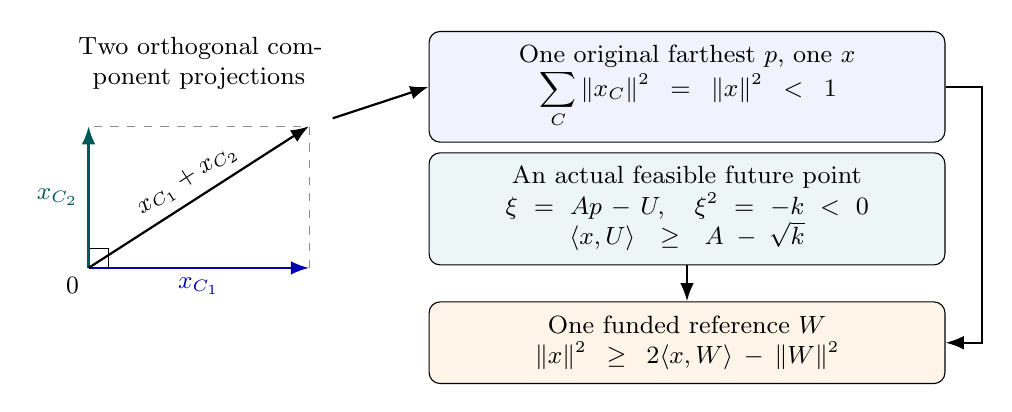
\begin{tikzpicture}[font=\small,>=Latex,
 box/.style={draw,rounded corners,align=center,text width=6.2cm,
 minimum height=.95cm,inner sep=5pt}]
 \coordinate (o) at (.4,.9);
 \coordinate (a) at (3.2,.9);
 \coordinate (b) at (.4,2.7);
 \coordinate (ab) at (3.2,2.7);
 \draw[->,thick,blue!70!black] (o)--(a)
   node[midway,below] {\(x_{C_1}\)};
 \draw[->,thick,teal!70!black] (o)--(b)
   node[midway,left] {\(x_{C_2}\)};
 \draw[->,thick] (o)--(ab)
   node[midway,above,sloped] {\(x_{C_1}+x_{C_2}\)};
 \draw[dashed,black!45] (a)--(ab)--(b);
 \draw (.65,.9)--(.65,1.15)--(.4,1.15);
 \node[below left] at (o) {\(0\)};
 \node[align=center,text width=4.1cm] at (1.8,3.5)
   {Two orthogonal component projections};
 \node[box,fill=blue!5] (budget) at (8.0,3.2)
   {One original farthest \(p\), one \(x\)\\
    \(\displaystyle\sum_C\|x_C\|^2=\|x\|^2<1\)};
 \node[box,fill=teal!7] (point) at (8.0,1.65)
   {An actual feasible future point\\
    \(\xi=Ap-U,\quad \xi^2=-k<0\)\\
    \(\langle x,U\rangle\ge A-\sqrt{k}\)};
 \node[box,fill=orange!9] (reference) at (8.0,-.05)
   {One funded reference \(W\)\\
    \(\|x\|^2\ge2\langle x,W\rangle-\|W\|^2\)};
 \draw[->,thick] (3.5,2.8)--(budget.west);
 \draw[->,thick] (point)--(reference);
 \draw[->,thick] (budget.east)--(11.75,3.2)
   --(11.75,-.05)--(reference.east);
\end{tikzpicture}
\caption{The orthogonal decomposition in $p^\perp$ and the point
estimate of Lemma~\ref{compact:lem:pointpressure}. Contributions from
the components are combined using the same vector.}
\label{compact:fig:ill20261026:c17:budget}
\end{figure}
% END ILLUSTRATION_20261026_C17_BUDGET
\section{Quadratic estimates from reference vectors}
\label{compact:sec:references}
The elementary estimate behind every certificate is
 \begin{equation}
\label{compact:eq:square}
 \norm{x}^2\geq2\ip{x}{W}-\norm{W}^2.
\end{equation}
Every term in \(\ip{x}{W}\) must be justified.
Write \(w=\sum_i b_iP_i\), \(b_i\geq0\), with actual pressures
 \(\ip{x}{P_i}>a_i\), and demand \(A_w=\sum_i b_i a_i\).
For a new actual pressure \(\ip{x}{Z}\geq h\), choose
 \[
 Q=Z-\sum_i t_iP_i,\qquad W=w+\mu Q.
\]
Before using pressures require \(\mu\geq0\) and check every
 \(b_i-\mu t_i\geq0\).
Then
 \begin{equation}
\label{compact:eq:payment}
 \ip{x}{W}\geq A_w+\mu(h-\sum_i t_i a_i),\quad
 \norm{W}^2=\norm{w}^2+2\mu\ip{w}{Q}+\mu^2\norm{Q}^2.
\end{equation}
The available price \(b_i\) is individual to anchor \(i\).
The first inequality is strict if some strictly constrained old
anchor retains a positive coefficient, or if \(\mu>0\) and the
new pressure is strict. For multiple corrections every new weight
must be nonnegative; their combined debit at each anchor and all
mutual cross terms must be retained.

Put \(P_i=e_1+\cdots+e_i\), \(S_i=\ip{x}{P_i}\).
If selected indices satisfy \(S_i>f_i\), concave interpolation
through \((0,0)\) and the selected \((i,f_i)\) gives a reference
whose coordinates are successive slopes. Its \(P_i\) coefficients
are successive slope decreases, hence nonnegative; its demand
is its squared norm. Omitting one unknown internal floor replaces
two adjacent slopes by their average, losing half their squared
difference. For \(\sqrt t\) at \(t\geq5\), the loss is less than
 \(1/3200\). Nonadjacent omissions have disjoint open intervals,
so losses add. A missing floor has coefficient zero.
References are Euclidean vectors, not asserted actual points:
actual points prove pressures, then positive coefficients combine
them in \eqref{compact:eq:square}.

\section{Component estimates}
\label{compact:sec:components}
\subsection{Ordinary components and exceptional actual defects}
All bounds below concern the same original projection, with
arbitrary finite spectators.
\begin{center}\small
\begin{tabular}{ll@{\qquad}ll}
\toprule
Component&Energy greater than&Component&Energy greater than\\ \midrule
ordinary nonshort \(A_1\)&\(1/10\)&ordinary \(A_2\)&\(319/2000\)\\
ordinary \(I_2(m),m\geq4\)&\(1/7\)&\(A_3\)&\(1/4\)\\
\(B_3,H_3\)&\(2/7\)&\(A_4\)&\(2/7\)\\
\(B_4,D_4,F_4\)&\(1/3\)&\(H_4\)&\(11/36\)\\
\(A_5\)&\(3/8\)&\(A_6\)&\(3/7\)\\
\(B_5,B_6\)&\(3/7\)&\(D_5,D_6\)&\(5/14,\ 3/7\)\\
\(B_7,D_7\)&\(1/2\)&\(B_8,D_8\)&\(4/7\)\\
\(E_6,E_7,E_8\)&\(9/20,\ 5/9,\ 2/3\)&&\\ \bottomrule
\end{tabular}
\end{center}
An actual isolated dotted short \(A_1\) is denoted \(I\).
A second short-wall profile \(J\) uses two old \(A_1\) factors
whose joint energy exceeds \(.34\).
The two typed rank-two exceptions, each of energy \(>.09\), are
 \[
 N_7=(\text{old }A_2,\ \text{new isolated native }7),\qquad
 O_7=(\text{old }I_2(7),\ \text{new isolated native }3).
\]
A bare \(I_2(7)\) is not automatically \(O_7\).
There is at most one short \(I/J\) profile or one typed exception;
they do not coexist. Acuteness of their actual isolated walls
is essential: two on orthogonal supports would have product
 \(-\sqrt{h_1h_2}\) strictly between \(-1/2\) and \(0\).
Appendix~\ref{compact:app:ordinary} proves the endpoint estimates,
the \(J\) case and the ordinary rates.

Useful joint bounds, counting \(I\) only once, are
 \begin{equation}
\label{compact:eq:joint}
 I+A_1>1/5,\quad I+2A_1>3/10,\quad
 I+T_2>21/100,\quad I+T_3>2/7.
\end{equation}
Here \(T_j\) is ordinary irreducible of rank \(j\).
Both typed exceptions force another \(T_2\) to cost \(>1/5\).
Another \(A_1\) costs \(>1/5\) beside \(N_7\) and \(>2/15\)
beside \(O_7\). For the latter, isolated height
 \(h=\tfrac14\csc^2(\pi/7)-1<1/3\) gives squared full tangent
greater than \(3/7\). Squared half tangent exceeds \(2/15\),
since \(4(2/15)/(1+2/15)^2=120/289<3/7\).
This is a real geometric argument.
The complete contact and defect proofs, including the actual-wall
height constraints behind \eqref{compact:eq:joint}, are given in
Appendix~\ref{compact:app:ordinary}. The uniform actual \(B/D\) floor
is proved in Appendix~\ref{compact:app:BDfloor}.

\subsection[The A-chain branch]{The \(A\)-chain branch}
For \(A_r\), use the zero-sum subspace of \(\R^{r+1}\) with roots
 \((e_i-e_{i+1})/\sqrt2\). The inverse Gram matrix is
 \[
 C_{ij}=\frac{2\min(i,j)(r+1-\max(i,j))}{r+1}.
\]
A finite-white classification of actual opposite walls gives
strong dual floors except for a short list of literal helper caps.
Adjacent weak helpers are excluded using their actual mutual
product and a positive two-cap projection. Concave interpolation
uses only strong floors; helper pressures are paid at surviving
anchors. The small end variance yields stronger component bounds:
\[
\begin{array}{c|ccccc}
r&r\geq7&r\geq8&r\geq13&16&17\\ \hline
e(A_r)>&1/2&4/7&5/7&199/250&6/7
\end{array}
\qquad e(A_{18})>91/100.
\]
Later local refinements give \(e(A_{12})>13/20\) and
 \(e(A_{15})>413/500\), uniformly with arbitrary spectators.
The shared actual feet, common-pair inventories, uniform
 \(1/2,4/7,5/7\) bounds, and the \(N=17,18,19\) central-window
and paid-reference arguments are proved in Appendix~\ref{compact:app:Achain}.
The newer \(A_{16}>.86\) proof in particular implies the older
 \(.796\) bound without requiring its separate historical reference.
The fresh smaller-rank proofs are in Sections~\ref{compact:app:A12}
and~\ref{compact:app:A15}. Their full native-cosine inventories and
individual actual-helper payments are included. Later exact-\(17\)
research remains excluded.

\subsection[The common B/D prefix branch]{The common \(B/D\) prefix branch}
For \(B_r\), use long roots \((e_i-e_{i+1})/\sqrt2\), \(i<r\),
and short root \(e_r\). For \(D_r\), use the long chain and the
fork root \((e_{r-1}+e_r)/\sqrt2\). On a long initial segment,
\(\omega_i=\sqrt2P_i\), \(C_{ij}=2\min(i,j)\).
In type \(D\), \(x_1>\cdots>x_{r-1}>|x_r|\); the last
coordinate is signed and the forks are distinct actual duals.
\begin{proposition}[Generic prefix theorem]
\label{compact:prop:prefix}
Let \(6\leq M\leq16\). Suppose an actual component is \(B_r\),
\(r\geq M+5\), or \(D_r\), \(r\geq M+6\). Put
 \[
 f_i=\sqrt i-\frac{61}{100\sqrt2},\quad
 E_M=\frac{f_5^2}{5}+\sum_{i=5}^{M-1}(\sqrt{i+1}-\sqrt i)^2,
 \quad H_M=\left\lfloor\frac{M-5}{2}\right\rfloor.
\]
With arbitrary finite spectators,
\(\sum_{j=1}^{M+1}x_j^2>E_M-H_M/3200\).
\end{proposition}
\begin{proof}
Appendix~\ref{compact:app:prefixinventory} proves that a weak site
 \(5\leq i\leq M+1\) has a pure cap
 \[
 v=\gamma\omega_i+\omega_1/2,\quad
 A^2=2i\gamma^2+2\gamma-\tfrac12,\quad
 101/125<\gamma<6/5,
\]
with own label \(5\), finite label at least \(7\), or dotted own
contact, and no spectator contact. Actual weak sites are
nonadjacent. This is proved at these ranks, not transferred from
a whole-component exclusion.
If \(5\) is strong, choose a strong \(K=M\) or \(M+1\).
Interpolate through actual strong knots. Each missing internal
floor loses \(<1/3200\); at \(K=M+1\) the extra increment
 \((\sqrt{M+1}-\sqrt M)^2>1/(4M+2)\geq1/66\)
pays the possible extra omission.

If \(5\) is weak, the first-six-root point table in
Appendix~\ref{compact:app:prefixinventory} gives \(x_1>.5965\), and \(6\) is strong, with
 \(S_6>2.01815\). Interpolate through \((1,.5965),(6,2.01815)\)
and a later strong endpoint. The slopes decrease:
\(.5965,.28433\), then \(1/(\sqrt K+\sqrt6)<1/5\).
Its energy exceeds
 \[
 L_M=.7600299945+\frac{(\sqrt M-\sqrt6)^2}{M-6},
\]
the last term being zero at \(M=6\).
Now \(E_6<.7\). The \(k=M-6\) increments from \(6\) onward lie
in \((1/8,1/5)\), so their variance is at most
 \(k(1/5-1/8)^2/4\leq9/640\).
Thus \(L_M-E_M>.76-.7-9/640>0\), directly also at \(M=6\).
This proves the weak-\(5\) branch without first assuming strong \(5\).
\end{proof}
Appendix~\ref{compact:app:prefixinventory} supplies the complete
finite-white inventory, zero-own repair, actual two-cap
nonadjacency, all four weak-\(5\) pressures and continuous
seals, with every spectator retained. Its original rank
inequalities are part of the theorem. A short-tail continuation
at an excluded rank still requires its own new local proof.

\section{The remaining spherical diagrams}
\label{compact:sec:forests}
\subsection[A fresh cover in exact dimension 18]{A fresh cover in exact dimension \(18\)}
Call \(A_r\), \(r\geq7\), or \(B_r,D_r\), \(r\geq9\),
dominant. Each costs \(>1/2\), so at most one is possible.
With none the ordinary rank-over-\(14\) baseline, even allowing
the unique defect, exceeds \(1\). Exactly one is therefore present.
The fresh total-rank-\(18\) necessary cover is:
\begin{center}\small
\begin{tabular}{p{.14\linewidth}p{.75\linewidth}}
\toprule
Dominant&All retained spectator alternatives\\ \midrule
\(A_{12}\)&\(I+(A_5\text{ or }D_5)\), or \(N_7/O_7+T_4\)\\
\(A_{15}\)&ordinary \(A_3\); \(T_2+A_1\); \(I+T_2\); or \(O_7+A_1\)\\
\(A_{16}\)&ordinary \(T_2\); two ordinary \(A_1\); \(I+A_1\); or \(N_7/O_7\)\\
\(A_{17}\)&one ordinary nonshort \(A_1\), or \(I\)\\
\(A_{18}\)&none\\
\(B_{16}\)&\(N_7/O_7\)\\
\(B_{17}\)&\(I\)\\
\(B_{18}\)&none\\
\(D_{16}\)&\(N_7/O_7\)\\
\(D_{17}\)&one ordinary nonshort \(A_1\), or \(I\)\\
\(D_{18}\)&none\\ \bottomrule
\end{tabular}
\end{center}
Here ordinary \(T_2=I_2(m)\), \(m\geq3\), and
 \(T_4\in\{A_4,B_4,D_4,F_4,H_4\}\).
\(H_4\) and native \(5\) are not discarded by field arguments.

For completeness, the accounting steps are as follows.
\(A_7\) leaves too many ordinary ranks;
\(A_8,\ldots,A_{11}\) are excluded by \(4/7\) plus
the rank-over-\(14\) baseline.
Beside \(A_{12}\), ordinary or \(J\) rank-six spectators cost
 \(>3/7\). With \(I\), \eqref{compact:eq:joint} excludes all rank-five
partitions except \(A_5,D_5\). With a typed exception, partition
rank \(4\): two \(T_2\)'s cost \(>.4\), \(T_3+A_1\) costs
 \(>1/4+2/15\), and the other reducible partitions are stronger.
Only irreducible \(T_4\) remains. For \(A_{13},A_{14}\),
the \(5/7\) bound and \eqref{compact:eq:joint} exclude all spectators.
At \(A_{15}\), exclude \(B_3,H_3\), three ordinary \(A_1\)'s,
\(I+2A_1\), \(J+A_1\), and \(N_7+A_1\).
At \(A_{16}\), \(.796\) excludes \(J\) but retains precisely
the listed rank-two alternatives. At \(A_{17}\) retain the
remaining \(A_1\).

For \(B_r,D_r\), the \(9/14\) bound forces spectator rank
at most \(5\), hence \(r\geq13\).
Proposition~\ref{compact:prop:prefix}, within its rank domain, gives
 \[
\begin{array}{c|rrrr}
r&13&14&15&16\\ \hline
e(B_r),e(D_r)>&.7349975&.7683275&.797425&.823735.
\end{array}
\]
At \(13,14,15\), every ordinary, \(I/J\), and typed remainder
exceeds the residual budget; \(I+T_2>.21\) closes rank \(15\).
At \(16\), two ordinary \(A_1\)'s and \(I+A_1\) are excluded;
ordinary \(T_2\) and both typed defects initially remain.
The \(B_3,D_4,D_3\) layer checks in
Appendix~\ref{compact:app:exact18layers} extend helper coverage to \(13\), giving
energy \(>.8689525\); ordinary \(T_2>1/7\) closes that case.
The fresh \(B_{17}\) layers reach a strong \(14/15\) endpoint
and energy \(>.90715\), excluding a nonshort ordinary \(A_1\).
This reuses the interpolation proof after new local coverage,
not Proposition~\ref{compact:prop:prefix} outside its legal ranks.

The first rows close with small shared consumers:
\[
 A_{12}+I+(A_5/D_5)>13/20+5/14=141/140,\quad
 A_{12}+N_7/O_7+T_4>13/20+.09+2/7=359/350.
\]
The improved \(413/500\) bound closes every \(A_{15}\) family:
ordinary total rank three costs \(>17/70\), \(I+T_2>.21\),
and beside \(O_7+A_1\) the total exceeds \(787/750\).
Thus the older separate ordinary-rank-three consumer is unnecessary.
The other internal proof homes are:
\begin{center}\small
\begin{tabular}{lp{.69\linewidth}}
\toprule
Row&Excluding project argument\\ \midrule
\(A_{16}\)&Proposition~\ref{compact:app:prop:A16}, ordinary and \(I+A_1\);
 Appendix~\ref{compact:app:A16typed18}, both actual typed defects\\
\(A_{17}\)&Appendix~\ref{compact:app:A17rankone18}, ordinary and actual \(I\)\\
whole \(A_{18}\)&Appendix~\ref{compact:app:wholeA18}, full two-end native-gap argument\\
\(B_{16}\)&Appendix~\ref{compact:app:BD16typed18}, both actual typed defects\\
\(B_{17}\)&Appendix~\ref{compact:app:B17I18}, actual \(I\); local head and helper kernels\\
\(D_{16}\)&Appendix~\ref{compact:app:BD16typed18}, both actual typed defects\\
\(D_{17}\)&Appendices~\ref{compact:app:D17ordinary18} and~\ref{compact:app:D17I18},
 ordinary and actual \(I\)\\
whole \(B_{18}\)&Section~\ref{compact:sec:b18}\\
whole \(D_{18}\)&Sections~\ref{compact:sec:d18-setup}--\ref{compact:sec:composition}\\
\bottomrule
\end{tabular}
\end{center}
Appendix~\ref{compact:app:exact18layers} proves the local layers used in
this cover, including the distinct signed \(D_4/D_3\) forks and the
actual \(A_{17}\) neighbor for \(B_{17}\). The table identifies the
complete proof of every retained row, including both short rank-one
cases. The independent higher-dimensional exclusions are proved in
Appendices~\ref{compact:app:highertail}--\ref{compact:app:exact19:wholeD19proof}.
These arguments use no field, lattice or integral dotted-product
hypothesis.

\subsection{The separate complete higher-dimensional tail}
\label{compact:subsec:higher}
The exact-\(18\) cover does not exclude higher dimensions.
The earlier internal package establishes the separate theorem:
\begin{theorem}[Internal higher-dimensional exclusion]
\label{compact:thm:tail}
There is no compact hyperbolic Coxeter polytope of dimension at least \(19\).
\end{theorem}
Appendix~\ref{compact:app:highertail} proves the component caps, shared
windows and complete actual-rank exclusions from \(29\) through \(20\).
The published ceiling is used only at dimensions at least \(30\).
At dimension nineteen, Proposition~\ref{compact:app:tail:prop:exact19cover}
leaves whole \(A_{19},B_{19},D_{19}\). Their proofs occupy
Appendices~\ref{compact:app:exact19:wholeclassical}--\ref{compact:app:exact19:wholeD19proof}:
the \(A\) proof splits by the three weak-end patterns; the \(B\)
proof splits by its two exceptional terminal walls; and the \(D\)
proof splits by six head types after a common centre analysis.
Each case keeps one original vector and every spectator in its cover.
Section~\ref{compact:app:tail:completeconjunction} joins these exclusions.

The higher ranks have their own complete covers in
Appendix~\ref{compact:app:highertail}. The short \(B_3/B_2\) and \(D_4/D_3\)
continuations are proved before the prefix estimates that consume them.
Section~\ref{compact:app:tail:completeconjunction} combines these actual-rank
arguments with the published compact ceiling. This is a logical
conjunction of exclusions, not geometric dimension heredity.
No arithmetic theorem or field census enters that conjunction.

\section[The whole-B18 terminal partition]{The whole-\(B_{18}\) terminal partition}
\label{compact:sec:b18}
Classify the actual opposite of old node \(17\) without assuming
a strong head. Section~\ref{compact:app:B18inventory} leaves:
\begin{enumerate}[label=(\roman*)]
\item a pure far-three helper with finite own \(5\), finite own
 at least \(7\), or dotted own \(1<g<4/3\);
\item near-three with own \(6\);
\item no left contact, with short white label \(3,4,5,6,7,8\).
\end{enumerate}
All other isolated, left, bridge and affine/null roles are excluded
in that inventory. Sections~\ref{compact:app:B18finitefar}--\ref{compact:app:B18localA17}
exclude the first branch, and Section~\ref{compact:app:B18near6} excludes
the second. In the last branch, Sections~\ref{compact:app:B18noleft}--\ref{compact:app:B18conclusion}
exclude distinct terminal caps and then every common-cap role.
The last common cap is treated at its actual adjacent whole-\(A_{18}\)
vertex, with comparison \(11/8\); that vertex is never assumed farthest.

Thus an original farthest whole-\(B_{18}\) vertex cannot occur.
Appendix~\ref{compact:app:wholeB18} gives the complete finite-white inventory,
each terminal exclusion, all original-wall checks and the individual
coefficient payments. Together with the preceding row consumers,
this leaves only whole \(D_{18}\) at the selected original vertex.

\section[The last case: an actual whole-D18 vertex]{The last case: an actual whole-\(D_{18}\) vertex}
\label{compact:sec:d18-setup}

We treat the final dotted-head case using the complete inventory
proved in Appendix~\ref{compact:app:D18foundation}.
Keep the original \(p,z,x\) and use actual old roots
 \[
 n_i=(e_i-e_{i+1})/\sqrt2\quad(1\leq i\leq17),\qquad
 n_{18}=(e_{17}+e_{18})/\sqrt2.
\]
Write
 \[
 P_i=e_1+\cdots+e_i,\quad
 \Omega_i=\sqrt2P_i\ (i\leq16),\quad
 \Omega_{17}=(P_{17}-e_{18})/\sqrt2,\quad
 \Omega_{18}=(P_{17}+e_{18})/\sqrt2.
\]
In particular \(x_{18}\) is signed and
 \(x_1>\cdots>x_{17}>|x_{18}|\). In this part only, set
 \begin{equation}
\label{compact:eq:d18floors}
 S_i=\ip{x}{P_i},\qquad f_i=\sqrt i-\frac{.58}{\sqrt2}.
\end{equation}
All terminating decimals in this paper denote exact rational numbers.

The head is the actual opposite wall of the long-end edge \(1\).
Section~\ref{compact:app:D18oldhead} proves that its normal is
 \[
 H=A_Hp-\eta\Omega_1,\qquad A_H^2=2\eta^2-1>0.
\]
The same section gives the complete own-contact list.
Sections~\ref{compact:app:D18strong16} and~\ref{compact:app:D18forkinventory} prove
the strong terminal floor \(S_{16}>f_{16}\), its funded reference
append and the complete fork-role list. The finite-head cases close
in Section~\ref{compact:app:D18foundationcomposition}.
We treat every dotted head \(\eta>1\) without a parameter cutoff.

Appendix~\ref{compact:app:D18foundation} proves these earlier inputs in
geometric dependency order: actual head isolation, the fresh threshold
window, strong \(16\), finite-head closure and the every-head pair
exclusions. In particular it proves the changed-threshold strong-site
statements afresh rather than inheriting them unconditionally.

\subsection{A future point valid for every dotted head}

Put \(u=\eta^{-2}\in(0,1)\), and consider
 \[
 \Xi=H+n_1/\eta.
\]
This is a positive combination of two actual normals.
Its products with \(H,n_1\) are respectively \(0\) and
 \(-\eta+1/\eta<0\), and \(\Xi^2=-(1-u)<0\).
Its time is \(A_H>0\). Every other actual wall has nonpositive
product with each summand. Hence its normalization is an actual
future point of the original polytope, with no unknown wall
omitted. Lemma~\ref{compact:lem:pointpressure} gives
 \begin{equation}
\label{compact:eq:headpoint}
 \ip{x}{Z_u}\geq h(u),\qquad
 Z_u=\frac{(2-u)e_1+u e_2}{2},\quad
 h(u)=\frac{\sqrt{2-u}-\sqrt{u(1-u)}}{\sqrt2}.
\end{equation}
Indeed the spatial part of \(\Xi\), divided by \(\sqrt2\eta\),
is \(Z_u\). We will use
 \[
 \sum_j(Z_u)_j=1,\qquad R(u)=\norm{Z_u}^2=1-u+u^2/2.
\]
Equation~\eqref{compact:eq:headpoint} is a point pressure, not an
energy lower bound, and is valid on the entire open interval.

\subsection{The four original reference cases}
\label{compact:subsec:fourrefs}

Section~\ref{compact:app:D18freshwindow} gives the following complete
initial alternatives: strong \(5\); a weak pure far-left-three
helper at \(5\); or an isolated dotted weak \(5\) with a chosen
strong \(J=6\) or \(7\). Thus there are four reference rows.
Here is why the initial classification has this precise scope.
Left own \(4\), including own \(4\)/white \(3\), gives a positive
actual affine-\(B\) null on the cap and old chain \(5,\ldots,18\);
the extra left contact preserves the remaining wall signs.
The newly possible near-three/own-five at \(5\) is excluded by
its actual right-\(H_4\) point and independent old strong
 \(11/12\), before the new references are used. Other finite-white
and isolated finite roles are strong. A historical fifth paid
row concerned a native-five head and is outside \(\eta>1\).

We emphasize the \emph{bare} references for the three nonhelper
rows. They interpolate through the strong knots, are flat on
their first \(J\) coordinates, and have endpoint sum \(f_{16}\).
Sections~\ref{compact:app:D18rawreferences} and~\ref{compact:app:D18strong16} give
 \[
\begin{array}{c|c|c|c|c}
\text{initial case}&B_0&\text{first mean }b<
 &\text{unused }P_J\text{ price}>&J\\ \hline
\text{strong }5&.9565188&.3652&.151&5\\
\text{isolated dotted }5,\ \text{strong }6&.9373243&.3399&.1435&6\\
\text{isolated dotted }5,\ \text{strong }7&.9196357&.31938&.1366&7
\end{array}
\]
More explicitly, each reference \(w\) has
 \[
 \ip{x}{w}>A_w,\quad 2A_w-\norm{w}^2>B_0,\quad
 \operatorname{supp}w\subset\{1,\ldots,16\},\quad
 \ip{w}{P_{16}}=f_{16},\quad \beta_{16}>.127.
\]
No head pressure has been paid. Their raw endpoint-\(15\)
lower bounds are \(.9403998,\allowbreak .9212053,\allowbreak .9035167\).
The legal endpoint-\(16\) append adds at least
 \(.127^2-.00001=.016119\); if \(15\) is weak, its fictitious
knot is deleted before pressure. All late repairs preserve the
flat first block and its individual prices.

In the isolated-\(5\) rows there is also an unused actual pressure
 \[
 U_5=P_5+\frac v2(e_6-e_5),\quad .4<v<1,\qquad
 \ip{x}{U_5}>1.8185.
\]
For
 \[
 Q_H=Z_u-P_J/J,\qquad Q_5=U_5-(5/J)P_J
\]
the exact identities are
 \begin{equation}
\label{compact:eq:flatresiduals}
 \norm{Q_H}^2=R-1/J,\quad
 \ip{Q_H}{Q_5}=1-5/J,\quad
 \norm{Q_5}^2<
 \begin{cases}77/150,&J=6,\\194/175,&J=7.\end{cases}
\end{equation}
Both residuals have zero product with the bare flat reference.
The positive mutual cross in \eqref{compact:eq:flatresiduals} will
not be discarded.

For the fourth row, the exact \emph{unheaded} weak-helper
reference interpolates from
 \((1,a_0)\), \(a_0=.5455\), to \((6,f_6)\), then through
the later actual strong knots to \(16\), replacing each missing
knot by a chord. Its first six coordinates are
 \begin{equation}
\label{compact:eq:helperbare}
 w_1=a_0,\quad w_2=\cdots=w_6=b_0=(f_6-a_0)/5.
\end{equation}
The actual helper proves \(x_1>a_0\) and strong \(6\).
The unheaded reference satisfies
 \[
 \ip{x}{w}>A_w,\quad L_w:=2A_w-\norm{w}^2>.987759,\quad
 \ip{w}{P_{16}}=f_{16},\quad \beta_{16}>.127.
\]
Weak \(7\), later omissions, and the late \(15\) repair do not
alter \eqref{compact:eq:helperbare}. Again no head pressure has been paid.
Appendices~\ref{compact:app:D18rawreferences}, \ref{compact:app:D18strong16}
and \ref{compact:app:D18finite78reference} supply the raw-reference increments,
omission tables, isolated-\(5\) pressure and individual coefficient
prices used here. These are internal geometric lemmas with written
proofs, not script-output assumptions.

\section{Bounds for the head and fork edges}
\label{compact:sec:uniformhead}

\subsection{The first three rows}
In the strong-\(5\) row choose \(\mu=.33\) on \(Q_H\).
Its debit \(.33/5=.066<.151\) fits the individual price.
Equations~\eqref{compact:eq:payment}--\eqref{compact:eq:flatresiduals} give
 \[
 L_W>.9565188+.66(h-.3652)-.1089(R-1/5)
       =F(u):=.7372668+.66h(u)-.1089R(u).
\]
For isolated \(5\) with \(J=6\), use weights
 \(\mu=.33,\nu=.10\) on \(Q_H,Q_5\).
The combined debit at \(J\) is \(.83/6<.1435\).
For \(J=7\) use \(\mu=.33,\nu=.11\), with debit
 \(.88/7<.1366\). In each case all remaining old coefficients
are nonnegative \emph{before} the new pressures are invoked, and
 \begin{align}
\label{compact:eq:isolatedfunding}
 L_W>{}&B_0+.66(h-b)+2\nu(1.8185-5b)
       -.1089(R-1/J)\notag\\
 &-\nu^2\norm{Q_5}^2-.66\nu(1-5/J).
\end{align}
{\raggedright
The constant terms before \(.66h-.1089R\) in the two rows are
 \(22164209/30000000\) and \(51729823/70000000\), both
greater than \(.7372668\). Thus \(F\) is a common lower bound.
No optimized helper and head energies have been added.\par}

We prove the bound uniformly on \(0<u<1\). Put
 \(a=\sqrt{2-u}\), \(b=\sqrt{u(1-u)}\). Direct differentiation gives
 \begin{equation}
\label{compact:eq:hcurvature}
 h''(u)=\frac{1/(4b^3)-1/(4a^3)}{\sqrt2}
        >\frac7{4\sqrt2},
\end{equation}
because \(b\leq1/2\), \(a>1\). Hence
 \(F''>.66\cdot7/(4\sqrt2)-.1089>.7\), using \(\sqrt2<1.415\).
At \(u_0=2/3\),
\[
\begin{gathered}
 h(u_0)=\sqrt{2/3}-1/3,\quad R(u_0)=5/9,\quad F(u_0)>.9956502,\\
 F'(u_0)=.2013-.0825\sqrt6,\quad |F'(u_0)|<.0008.
\end{gathered}
\]
The value bound uses
 \(.81649^2=.6666559201<2/3\), and the derivative bound uses
 \(2.4494<\sqrt6<2.4495\). Taylor's inequality and completion
of the square on the segment between \(u_0\) and \(u\) give
 \begin{equation}
\label{compact:eq:Fseal}
 F(u)>.9956502-\frac{.0008^2}{1.4}>.99564
 \qquad(0<u<1).
\end{equation}
No endpoint derivative or sampled minimum is used.

\subsection{The weak-helper row: two separate anchor prices}
\label{compact:subsec:helperfunding}
The unheaded reference \eqref{compact:eq:helperbare} has two available
prices
 \begin{equation}
\label{compact:eq:twoprices}
 \beta_1=a_0-b_0>.24672,\qquad
 \beta_6\geq b_0-(\sqrt7-\sqrt6)>.1023.
\end{equation}
Indeed \(2.0392<f_6<2.0394\), so
 \(.29874<b_0<.29878\), while
 \(\sqrt7-\sqrt6<2.6458-2.4494=.1964\).
An adjacent omitted knot decreases the next slope and increases
 \(\beta_6\). The bounds follow from
 \(2.4494<\sqrt6<2.4495\) and
 \(.4101<.58/\sqrt2<.4102\), by positive squaring.

Define
 \[
 Q=Z_u-(1-3u/5)e_1-(u/10)P_6.
\]
Its first coordinate is zero, its second is \(.4u\), and its
third through sixth coordinates are \(-.1u\). Therefore
 \begin{equation}
\label{compact:eq:helperresidual}
 \norm{Q}^2=u^2/5,\qquad \ip{w}{Q}=0.
\end{equation}
Choose \(\mu=.22\). First pay the \emph{separate} anchor debits
 \[
 \mu(1-.6u)<.22<\beta_1,\qquad
 \mu u/10<.022<\beta_6
 \quad(0<u<1).
\]
The remaining original coefficients are nonnegative. Only then
add the positive new head pressure \(\mu Z_u\).
The terminal coefficient at \(16\) remains unused. The full
one-vector square gives
 \begin{align}
\label{compact:eq:Gdefinition}
 L_{w+\mu Q}
 &>.987759+.44[h-a_0+(3a_0/5-f_6/10)u]-.00968u^2\notag\\
 &>G(u):=.747739+.44h(u)+.0542784u-.00968u^2,
\end{align}
since \(3a_0/5-f_6/10>.12336\).
This argument rewrites a positive-coefficient pressure
decomposition before using it; it does not subtract old lower
floors from an unknown signed pressure.

We give the exact small-margin seal. By \eqref{compact:eq:hcurvature},
\(G''>.44\cdot7/(4\sqrt2)-.01936>.5\).
At \(u_1=.642\), positive square tests give
 \[
 \sqrt{1.358}>1.1653325,\qquad
 \sqrt{.229836}<.4794122,
\]
whose comparison squares are \(1.35799983555625\) and
 \(.22983605750884\). The difference exceeds \(.6859203\).
Since
 \[
 .4850188\cdot1.4142136=.68592018321568<.6859203,
 \qquad1.4142136^2>2,
\]
we have \(h(.642)>.4850188\), and hence
 \[
 G(.642)>.99200425728.
\]
For the derivative use
 \[
 .858<1/\sqrt{1.358}<.859,\quad
 .592<.284/\sqrt{.229836}<.593,\quad
 .353<1/(2\sqrt2)<.354.
\]
They follow by multiplying the positive radical brackets
 \(1.1653<\sqrt{1.358}<1.1654\) and
 \(.4794121<\sqrt{.229836}<.4794122\).
Thus
 \[
 -.094518<h'(.642)<-.093545,\qquad
 .00026136<G'(.642)<.00068948<.0007,
\]
because \(G'=.44h'+.0542784-.01936u\).
Strong convexity on the entire interval now gives
 \begin{equation}
\label{compact:eq:Gseal}
 G(u)>.99200425728-.0007^2
       =.99200376728>.992.
\end{equation}

Combining \eqref{compact:eq:Fseal} and \eqref{compact:eq:Gseal}, every one of
the four original initial cases supplies a single legally
funded reference \(W\) with
 \begin{equation}
\label{compact:eq:uniformcontract}
 L_W>.992,\quad
 \operatorname{supp}W\subset\{1,\ldots,16\},\quad
 \ip{W}{P_{16}}=f_{16},\quad
 \text{unused }\beta_{16}>.127.
\end{equation}
All corrections have sum zero and support at most \(7\);
the late omissions and the original endpoint-\(16\) price survive.

\subsection{Both signed fork directions}
\label{compact:subsec:forkheight}
Let \(\Delta=S_{16}-f_{16}\geq0\). The pressure decomposition
of \(W\) keeps its original terminal coefficient. Therefore
 \(\ip{x}{W}>A_W+\beta_{16}\Delta\), and the same norm identity
gives
 \begin{equation}
\label{compact:eq:slack}
 \norm{x-W}^2<.008-.254\Delta,\qquad
 x_{17}^2+x_{18}^2<.008-.254\Delta.
\end{equation}
The two true unit fork duals are
 \[
 \frac{\Omega_f}{3}
   =\frac{P_{17}\pm e_{18}}{\sqrt{18}},
 \qquad f=17,18.
\]
For either actual fork height,
\begin{align}
\label{compact:eq:truefork}
 t_f:=\ip{x}{\Omega_f/3}
 &<\frac{f_{16}+\Delta+\sqrt{.016-.508\Delta}}{\sqrt{18}}\notag\\
 &<\frac{3.59+.1265}{\sqrt{18}}<.876.
\end{align}
The numerator decreases with \(\Delta\): its derivative is
 \(1-.254/\sqrt{.016-.508\Delta}<0\) on its nonempty domain.
The endpoint is handled by continuity. The seals are
 \(f_{16}<3.59\), \(\sqrt{.016}<.1265\),
\(\sqrt{18}>4.2426\), and
 \(.876\cdot4.2426=3.7165176>3.7165\).
No absolute value has replaced the signed last coordinate.

For an actual fork edge with distance cosine \(C\),
\eqref{compact:eq:halfheight} gives
 \(t_f\geq\sqrt{(C-1)/(C+1)}\). Hence
 \begin{equation}
\label{compact:eq:forkcosh}
 C<\frac{1+.876^2}{1-.876^2}<7.6,
\end{equation}
since \(.876^2=.767376\) and
 \(7.6\cdot.232624=1.7679424>1.767376\).
In Section~\ref{compact:app:D18forkinventory}, every far-next-three
role has \(g\geq\cos(\pi/5)>.809\) and exact cosine
 \(C=9g+1>8.281\). Equation~\eqref{compact:eq:forkcosh} removes that
entire role, including all its previously classified native/null
own alternatives.

\section[A local A18 lemma at an adjacent actual vertex]{A local \(A_{18}\) lemma at an adjacent actual vertex}
\label{compact:sec:localA18}
\begin{lemma}
\label{compact:lem:localA18}
Let \(q\) be an actual vertex of a compact Coxeter
 \(18\)-polytope whose whole incident diagram is \(A_{18}\).
Write \(z=E_q(q-y)\), \(\norm{y}<1\). Suppose
 \[
 -\ip{z}{r}\leq\kappa E_q
 \quad\text{for every actual point }r\text{ of the original }P,
 \qquad\kappa<11/8.
\]
Then \(\ip{y}{u_{18}}>.78\) is impossible for the positive
normalized endpoint-dual direction.
\end{lemma}
The lemma is local at \(q\), which is not assumed farthest.
Appendix~\ref{compact:app:localAinputs} supplies its local inventory; no
original \(B_{18}\) hypothesis is used.
\begin{proof}
In the zero-sum subspace of \(\R^{19}\), for \(i\leq j\),
\[
 D_i=\norm{\omega_i}^2=\frac{2i(19-i)}{19},\qquad
 C_{ij}=\frac{2i(19-j)}{19}.
\]
Call \(5\leq i\leq14\) weak if
 \(\ip{y}{\omega_i}\leq\sqrt{D_i}-.87\).
The complete inventory at comparison \(11/8\), established
before any endpoint pressure, leaves only:
\begin{enumerate}[label=(\alph*)]
\item near-four, meaning own \(4\) and white \(3\) at the adjacent
 old node, in the four literal side-order-\(5/6\) orientations;
\item a pure far-end-three helper
 \[
 d_i=A_iq-\gamma_i\omega_i-\omega_e/2,\quad
 e=1\text{ or }18,\quad
 \varphi/2\leq\gamma_i<17/16,
\]
 with own \(5\), finite own at least \(7\), or dotted own.
\end{enumerate}
Here \(\varphi=(1+\sqrt5)/2\).
All isolated caps are strong. The inventory includes own zero,
every finite own, parallel and unbounded dotted owns.
Every positive point checks every unknown original wall.

Some calculations locate the numerical boundary.
Every ordinary edge ratio at least \(3/2\) is strong:
with \(a=3/2,k=11/8\), the square comparison for
 \(q_0=\sqrt{D_i}\in[2.7,3.1]\) is the positive polynomial
 \[
 -.21q_0^3+1.1876q_0^2-1.74q_0+.7569.
\]
It is concave with endpoint values \(.583074,.519626\).
The near-four ratio of side order \(\ell\) is
 \[
 \frac{1/\sqrt2+(\ell-1)/(2\ell)}
      {\sqrt{(\ell+1)/(2\ell)}}.
\]
It increases in \(\ell\) and exceeds \(3/2\) at \(\ell=7\),
since \((67+42\sqrt2)/56>9/4\). Only \(i=5,6\) with white
 \(i-1\), and \(i=14,13\) with white \(i+1\), can be weak.
For pure helpers the identity
 \[
 \frac{(\gamma+1/(2\ell))^2}{(\ell+1)/(2\ell)}
 -(4\gamma-2)
 =\frac{(\gamma-1-1/(2\ell))^2}{(\ell+1)/(2\ell)}\geq0
\]
gives the stated cutoff at the weakened comparison.

The local input retains genuine helper nonadjacency at this
factor. Its proof uses the following exact actual products.
For adjacent helper owns \(A,B\in[.808,1.08]\), the mutual
product \(R\) satisfies
 \[
\begin{array}{c|l}
\text{same end}&R\geq1-\frac{18}{19}AB-\frac{|A-B|}{19}>-1/2\\
\text{outward}&R\geq\frac12-AB+\frac{(A-1)(B-1)}{19}>-.7\\
\text{reversed}&R\geq\frac12-AB+\frac{(A+1)(B+1)}{19}>-.7.
\end{array}
\]
The native alphabet leaves \(R=0\) in the first case and
 \(R=0,-1/2\) in the others. Outward \(R=0\) contradicts
 \[
 (D_i-4/5)(D_{i+1}-4/5)-C_{i,i+1}^2
 =\frac25 C_{i,i+1}-\frac{24}{25}+\frac8{95}
 \geq884/475>0.
\]
For reversed \(R=0\), set \(l=i,r=18-i\).
The exact determinant would require
 \[
 4lr A^2B^2-(l+1)(r+1)(A^2+B^2)-2AB
 -(l+1)A-(r+1)B+21/4=0.
\]
Its own derivatives are positive on that rectangle.
If one own is not \(5\), it exceeds \(.9\); evaluating the
other at \(.808\), the endpoints \(l=5,13\) give
 \(.9601824,1.6961824>0\), and concavity in \(l\) excludes all.
For two native-five owns the norm-two calculation in basis
 \(1,\varphi\) has nonzero rational determinant coefficient
 \(475\) outward and \(-361\) reversed. This uses only native
cosine algebra. Thus remaining products are \(0\) for a
common helper and \(-1/2\) for opposite helpers.

After clearing old roots, the actual two-cap Schur matrices
are \(I-t\mathbf1\mathbf1^T\), \(t=(\ell-1)/(2\ell)\), or
the matrix with diagonal
 \(\delta_l,\delta_r\in(1/2,3/5]\), off-diagonal \(-1/2\).
Both are positive with positive inverse. Their positive
projections are feasible against every original wall,
including the reverse wall at \(q\).
The cap-time and weight estimates in Appendix~\ref{compact:app:localAinputs} give
weighted mean loss less than
 \[
 1/10+(11/8)(7/16)=.7015625
 \quad\text{or}\quad1/10+(11/8)(3/10)=.5125.
\]
Both are less than \(.87\), excluding adjacent weak helpers.
None of these steps uses endpoint height \(>.8\).

Now assume the new height \(\ip{y}{u_{18}}>.78\).
Each weak near-four has an actual mate, formed by releasing
its white neighbor and retaining its cap. Positive finite
Gram inversion gives an actual adjacent vertex feasible
against every wall. Its edge cosine exceeds \(11\);
for example the left mates have
 \[
 C_j=\sqrt{2(i-1)/19}
 \left((20-i)/2+(19-i)/\sqrt2\right)>11,\qquad i=5,6.
\]
At comparison \(11/8\), the normalized mate height exceeds
 \(7/8\). A left mate has correlation \(<.15\) with \(u_{18}\).
The sum of these heights exceeds \(1.655\), whose square
exceeds \(2.3\), while the squared norm of the sum of the
directions is \(<2.3\). This contradicts \(\norm{y}<1\).
No left near-four remains.

Some \(k=5,6\) is now strong by helper nonadjacency, with
normalized height \(>.677\).
For a right mate \(j=14,15\), the correlation formula
 \[
 \rho_{ab}=\sqrt{\frac{a(19-b)}{b(19-a)}}\quad(a\leq b)
\]
gives \(\rho_{18,j}<.46,\rho_{18,k}<.161,\rho_{j,k}<.407\).
For one vector \(V=.5u_{18}+.6u_j+.4u_k\),
\[
 \ip{y}{V}>.5(.78)+.6(7/8)+.4(.677)=1.1858,\quad
 \norm{V}^2<.77+.276+.0644+.19536=1.30576.
\]
Equation~\eqref{compact:eq:square} gives \(\norm{y}^2>1.06584\).
All near-four orientations are excluded at \(.78\).
Only nonadjacent pure weak helpers remain.

Use rational heights \(H_{19-i}=H_i\), linear on \(0\)--\(5\)
and \(14\)--\(19\), with
 \[
 H_5=1.844,\ H_6=1.995,\ H_7=2.103,\ H_8=2.173,\
 H_9=H_{10}=2.207.
\]
Their positive slopes are \(.3688,.151,.108,.070,.034\),
then zero. The squares \((H_i+.87)^2\), \(5\leq i\leq9\), are
 \[
 7.365796,\ 8.208225,\ 8.838729,\ 9.259849,\ 9.467929,
\]
strictly below \(140/19,156/19,168/19,176/19,180/19\).
Thus every retained positive dual is paid by a strong floor.
If \(5\) is weak use chord \(0\)--\(6\), reflect at \(14\),
and omit each internal weak knot by its neighbor chord.
After chords set \(w_i=(H_i-H_{i-1})/\sqrt2\).
The reference is zero-sum with demand \(E_0=\norm{w}^2\).

Before internal holes, the exact energies for zero, one and
two weak ends are \(.7205882,\allowbreak .70082285,\allowbreak .6810575\).
Internal curvatures are \(.043,\allowbreak .038,\allowbreak .036,\allowbreak .034\) and reflections;
even summing all eight losses gives
 \[
 2(.043^2+.038^2+.036^2+.034^2)/4=.0028725<.002873.
\]
Nonadjacency makes the losses legitimate. End chords do not
change any eligible internal curvature. Hence
 \begin{equation}
\label{compact:eq:Alocalbase}
 E_0>
 \begin{cases}
 .6781845,&14\text{ weak: }m=6,\ K=13,\ H_K=1.995,\\
 .69794985,&14\text{ strong: }m=5,\ K=14,\ H_K=1.844.
 \end{cases}
\end{equation}
The surviving individual anchor prices are
 \[
 \beta_{13}\geq(7H_6/6-H_7)/2=.11225,\qquad
 \beta_{14}\geq(6H_5/5-H_6)/2=.1089.
\]
Adjacent holes increase the anchor price. Omitted knots have
price zero; no missing strong \(7\) or \(18\) floor is paid.

Define
 \[
 G_0=-e_{19}+\frac1m\sum_{\text{last }m}e_i,
\]
with \(19\) included. Then
 \[
 \norm{G_0}^2=(m-1)/m,\quad \ip{w}{G_0}=0,\quad
 G_0=\omega_{18}/\sqrt2-\omega_K/(m\sqrt2).
\]
Use the new weight \(\mu=.6\).
The debit \(.6/(m\sqrt2)\) is \(<.071\) for \(m=6\),
\(<.085\) for \(m=5\), below the separate anchor prices.
The positive endpoint coefficient is paid by its actual height.
Here
 \[
 -y_{19}>.78\sqrt{18/19}>.7591,
\]
since \(19(.7591)^2=10.94842339<18(.78)^2=10.9512\).
The last-block means are
 \(H_K/(m\sqrt2)<.2352\) or \(<.261\).
The same local-\(y\) square, retaining \(\ip{w}{G_0}=0\), gives
 \[
\begin{array}{ll}
m=6:&\norm{y}^2>
 .6781845+1.2(.7591-.2352)-.36(5/6)=1.0068645,\\
m=5:&\norm{y}^2>
 .69794985+1.2(.7591-.261)-.36(4/5)=1.00766985.
\end{array}
\]
Both contradict \(\norm{y}<1\), proving the lemma with the
local inventory established in Appendix~\ref{compact:app:localAinputs}.
\end{proof}
Appendix~\ref{compact:app:localAinputs} supplies the complete
local own/white inventory, isolated-cap point bounds,
positive mixed weights and native-five determinant
expansion used above. It uses only real geometry and
comparison \(11/8\), with no original-\(B_{18}\) premise.
The original-\(x\) energy is never added to this local-\(y\) budget.

\section{The near/far pair and the final composition}
\label{compact:sec:composition}
\subsection{Every actual near/far fork edge is short}
For a near-three or far-three fork role, the complete finite-white
classification in Section~\ref{compact:app:D18forkinventory} gives an
actual other endpoint \(q\)
with whole diagram \(A_{18}\). The positive reverse direction
at \(q\) is exactly its normalized new endpoint dual: \(p\)
has nonzero product with only that new incident root.
Let \(C\) be the original edge cosine,
\(\beta=\sqrt{C^2-1}/C\), and \(t=t_f<.876\).

Suppose \(C\geq5.6\). Then
 \[
 E_q/E=C-\sqrt{C^2-1}\,t
       >5.6-.876(5.51)=.77324.
\]
The function increases for \(C\geq5.6\).
Here \(5.51^2=30.3601>30.36\) and
 \((11/8)(.77324)>1\), so \(E/E_q<11/8\).
Also \(\beta>.9839\), because
 \(31.36(1-.9839^2)=1.0016631744>1\).
The positive reverse height satisfies
 \[
 \ip{y}{u_{18}}=\frac{\beta-t}{1-\beta t}>.78.
\]
Its denominator is positive and its limiting gap is
 \[
 .9839-.876-.78(1-.9839\cdot.876)=.000179192>0.
\]
The original maximum supplies all-point comparison at \(q\).
Lemma~\ref{compact:lem:localA18} excludes \(C\geq5.6\).
Every actual near/far fork edge therefore has \(C<5.6\).

\subsection{The entire near/far family}
Suppose the actual fork opposites are near and far:
\[
 c_N=Np-\gamma\Omega_f-\Omega_o/2,\qquad
 c_F=Fp-\delta\Omega_o-\Omega_1/2,
\]
with \(f,o\) the different actual forks.
Their times and exact edge cosines are
 \[
 N^2=9\gamma^2+8\gamma+5/4,\quad
 F^2=9\delta^2+\delta-1/2,\quad
 C_N=\frac{18\gamma+8}{\sqrt{19}},\quad
 C_F=\frac{18\delta+1}{\sqrt{19}}.
\]
The short-edge bounds and \(\sqrt{19}<4.359\) give
 \(\gamma<.912,\delta<1.301\).
Put \(U=3\gamma+4/3,V=3\delta+1/6,a^2=19/36\).
Then \(N^2=U^2-a^2,F^2=V^2-a^2\), and
 \[
 (UV-a^2)^2-N^2F^2=a^2(U-V)^2\geq0,\qquad UV-a^2>0.
\]
The actual mutual magnitude consequently satisfies
 \begin{align*}
 \lambda=-\ip{c_N}{c_F}
 &=NF-8\gamma\delta-\gamma/2-(9/2)\delta-1/4\\
 &\leq\delta(\gamma-1/2)-5/9\\
 &<1.301(.412)-5/9=.536012-5/9<0.
\end{align*}
This contradicts all-wall acuteness. If \(\gamma\leq1/2\)
the upper bound is already negative; the accepted own list
in fact has \(\gamma\geq\cos(\pi/4)>1/2\).
Zero, every finite, parallel and unbounded dotted mutual
are excluded at once, for all finite or dotted near/far owns.

\subsection{Exhausting the actual head and fork covers}
For a dotted head, \eqref{compact:eq:forkcosh} removes every
far-next-three role from Section~\ref{compact:app:D18forkinventory}.
What remains is isolated, near-three, or far-three.
Their six unordered pairs are exhausted by
\begin{center}\small
\begin{tabular}{ll}
\toprule
Actual pair&Complete excluding argument\\ \midrule
isolated/isolated&Sections~\ref{compact:app:D18isolatedfinite} and~\ref{compact:app:D18isolateddotted}\\
isolated/near&Section~\ref{compact:app:D18isolatednear}\\
isolated/far&Sections~\ref{compact:app:D18isolatedfarfinite} and~\ref{compact:app:D18farpairexits}\\
near/near&Section~\ref{compact:app:D18forkinventory}\\
near/far&The complete argument above\\
far/far&Section~\ref{compact:app:D18farpairexits}\\ \bottomrule
\end{tabular}
\end{center}
Both assignments of the genuine signed forks are included.
Every pair is impossible, so no dotted head remains.

The head cover also includes own zero, finite and parallel
cases. Section~\ref{compact:app:D18oldhead} removes own
 \(0,3,4\) by time constraints and own \(6\) by a positive
affine \([6,3]\) kernel. At own \(6\) an actual null is
 \(\sqrt3H+2n_1+n_2\); at parallel own it is \(H+n_1\).
The remaining finite labels \(5,7,8,9\) and every integer
label at least \(10\) are excluded by the complete conjunction in
Section~\ref{compact:app:D18foundationcomposition}. Every dotted own has just been excluded.
Thus the whole-\(D_{18}\) diagram is impossible.

Theorem~\ref{compact:thm:tail} excludes every dimension at least \(19\).
At exact dimension \(18\), the fresh complete cover and its
row consumers, including Section~\ref{compact:sec:b18}, leave only
whole \(D_{18}\) at the same original farthest vertex.
The head/fork argument excludes it. Hence dimension \(18\)
is impossible, proving Theorem~\ref{compact:thm:main}. Each step uses its
own actual-rank cover and the same original vector within a case;
no dimension heredity is used.

% BEGIN ILLUSTRATION_20261026_C17_CONJUNCTION
\begin{figure}[tbp]
\centering
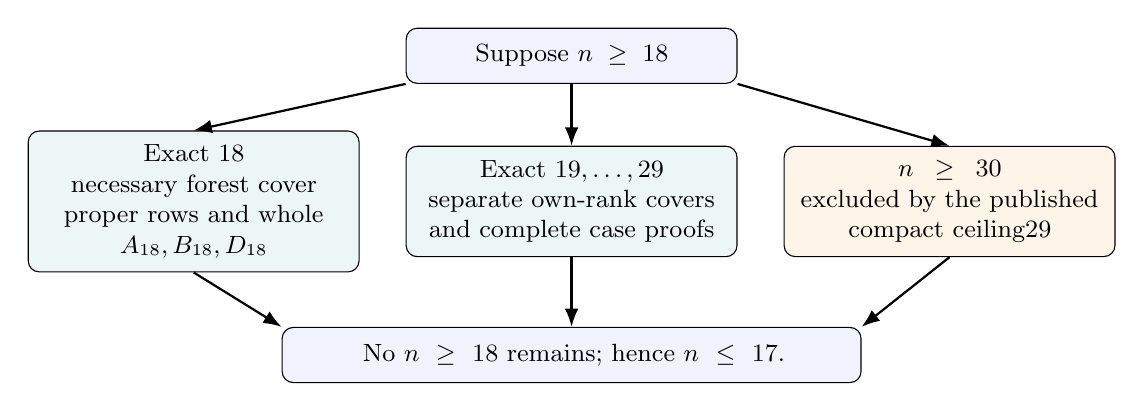
\begin{tikzpicture}[font=\small,>=Latex,
 box/.style={draw,rounded corners,align=center,text width=3.85cm,
 minimum height=1.4cm,inner sep=5pt}]
 \node[box,minimum height=.7cm,fill=blue!5] (start) at (6.7,3.85)
   {Suppose \(n\ge18\)};
 \node[box,fill=teal!7] (eighteen) at (1.9,2.0)
   {Exact \(18\)\\necessary forest cover\\proper rows and whole\\
    \(A_{18},B_{18},D_{18}\)};
 \node[box,fill=teal!7] (tail) at (6.7,2.0)
   {Exact \(19,\ldots,29\)\\separate own-rank covers\\and complete case proofs};
 \node[box,fill=orange!9] (published) at (11.5,2.0)
   {\(n\ge30\)\\excluded by the published\\compact ceiling29};
 \node[box,text width=7.0cm,minimum height=.7cm,fill=blue!5]
   (finish) at (6.7,.05)
   {No \(n\ge18\) remains; hence \(n\le17\).};
 \draw[->,thick] (start.south west)--(eighteen.north);
 \draw[->,thick] (start)--(tail);
 \draw[->,thick] (start.south east)--(published.north);
 \draw[->,thick] (eighteen.south)--(finish.north west);
 \draw[->,thick] (tail)--(finish);
 \draw[->,thick] (published.south)--(finish.north east);
\end{tikzpicture}
\caption{The compact dimension bound. The exclusion of dimension $18$
is combined with the higher-dimensional exclusions proved
in Section~\ref{compact:app:tail:completeconjunction}.}
\label{compact:fig:ill20261026:c17:conjunction}
\end{figure}
% END ILLUSTRATION_20261026_C17_CONJUNCTION
\section{Finite algorithms and conditional verification}
\label{compact:sec:verification}
\subsection{The mathematical finite-cover calculation}
The rank covers are finite combinatorial arguments supported
by real inequalities, not field enumerations.
For fixed total rank \(n\), the forest calculation is:
\begin{enumerate}
\item List partitions of \(n\) into ranks of spherical irreducibles.
 Retain all exceptional finite types and classical types at
 their actual ranks. Keep \(I_2(m)\) as a symbolic ordinary
 rank-two family for unbounded \(m\), distinguishing its
 exceptional actual typed profiles.
\item Mark at most one allowed \(I/J/N_7/O_7\) profile by the
 actual-wall compatibility lemma. Apply joint bounds only to
 disjoint sets of components, counting each defect once.
\item Sum proved same-vector energy bounds. Discard a forest only
 when a strict lower bound is at least \(1\). If a dominant
 rank needs a fresh local layer, retain it until that
 actual-rank lemma is established.
\item Return the retained grouped necessary cover and the
 inequality discarding every other partition.
\end{enumerate}
Termination follows from finitely many rank partitions and
finite type choices at each rank. The unbounded native
parameter is represented by inequalities proved over its
entire domain. Completeness uses spherical classification,
compact acute simplicity, complete actual-defect compatibility,
and spectator-uniform component bounds. The output is a
necessary cover; no realization follows. A program testing
only finitely many native labels would not establish it.

Local own/white calculations have a different domain.
After deleting a specified original node, classify every
finite extension of the retained spherical forest by its
actual opposite wall, including own zero, all finite owns,
parallel and dotted owns. Finite white extensions are bounded
by spherical classification. Infinite own families are closed
by analytic inequalities over complete intervals.
Termination of a finite classification does not justify
discarding a continuous branch. Completeness must include
spectator attachments, affine kernels and every original
wall for every auxiliary point.


\clearpage
\part{Compact arithmetic polytopes}\label{part:arith}




\section{The result and the common argument}\label{arith:sec:scope}

All polytopes are convex, finite-sided and full-dimensional.
Arithmeticity refers to the lattice generated by their facet reflections.

\begin{theorem}\label{arith:thm:main}
Every compact arithmetic hyperbolic Coxeter polytope has dimension at
most fifteen.
\end{theorem}

The argument separates geometry from arithmetic at a definite point.
Geometry provides one vector whose squared norm is less than one.
Its projections onto whole finite diagram components are constrained
by actual neighboring walls. Arithmeticity then limits the fields and
integral parameters of those walls. When pressures overlap, their coefficients are paid together
before one completed square is used.

\begin{proposition}[Compact dimension bound]\label{arith:prop:general17}
Every compact real hyperbolic Coxeter polytope has dimension at most
seventeen, without an arithmetic hypothesis.
\end{proposition}

The general compact bound is proved independently in Part~II.
It excludes dimension eighteen and every higher dimension,
so only dimensions seventeen and sixteen remain here. We first split by the whole finite forest; the final
 $D_{16}$ argument splits by the inert, ramified or split behavior of two.
No argument assumes arithmeticity or Coxeter angles for an arbitrary face.

Section~\ref{arith:sec:seventeen} gives the rank-seventeen reduction, and
Section~\ref{arith:sec:algorithms} states the finite algorithms and their
numerical output premises. Section~\ref{arith:sec:sixteen} gives the
rank-sixteen reduction; Sections~\ref{arith:sec:d16}--\ref{arith:sec:split} prove
the final dyadic obstruction. The appendices develop the component
estimates, actual-domain inclusions and complete forest dispatches
used in these reductions.

\subsection{One original vector}
Use the Lorentz form with negative time coordinate and outward unit
normals. Distinct actual wall normals have nonpositive products.
Compact acute simplicity gives a rank-$n$ finite spherical forest at
each vertex. Choose a strict interior point $z$ and an actual vertex
 $p$ farthest from it. Write
 \[
 z=E(p-x),\quad E>0,\quad x\in p^\perp,\qquad
 \|x\|^2=\sum_C e_C<1,\quad e_C=\|x_C\|^2.
\]
The sum is over whole orthogonal finite components. Overlapping
subdiagrams do not supply independent summands.
If $q=\cosh(L)p-\sinh(L)u$ is an actual adjacent vertex, then
 \begin{equation}\label{arith:eq:edge}
 x\cdot u\ge(\cosh L-1)/\sinh L=\tanh(L/2).
\end{equation}
More generally a future unit point $q=ap-v$, with $v\in p^\perp$,
satisfying every wall of the original polytope gives $x\cdot v\ge a-1$.
Distance from $z$ is convex on geodesic segments, so its maximum over
the compact polytope is attained at a vertex.
For any reference vector $w$,
\begin{equation}\label{arith:eq:square}
 \|x\|^2\ge2x\cdot w-\|w\|^2,
\end{equation}
by $\|x-w\|^2\ge0$.
Each coefficient removed from an original pressure must fit its
individual available coefficient. Positive combinations of actual
normals satisfy every unselected wall by acuteness; future orientation
and the finite or negative square still need proof. The companion
and the precisely cited supplements make these checks before using
\eqref{arith:eq:square}.

\subsection{What arithmeticity adds}
An arithmetic reflection lattice has an admissible quadratic-form
model over its actual totally real field $K$; the structural reflection
theorem is recorded as Lemma~5.2 of~\cite{ABSW}. It supplies $K$-valued
root lines and positive definite nonphysical forms. For roots $r_i$ on
those lines put
 \[
 a_{ij}=2(r_i,r_j)/(r_i,r_i).
\]
Invariant cyclic products are algebraic integers and generate the
actual ground field. Individual physical unit roots need not be
 $K$-valued. Disconnected roots need not have equal raw norm squareclasses.

If an actual principal Gram matrix, after its specified permitted
 $K$-rescaling, is defined over $k\subset K$ and indefinite physically,
then $K=k$: an additional real embedding fixing $k$ would preserve
indefiniteness and contradict positive definiteness.
A nonzero algebraic integer also has nonzero integral norm, so bounds
at \emph{every} nonphysical embedding can force a degree bound.
Neither argument assumes a convenient overfield or an integer power basis.

The rational field is excluded in the dimensions used here: compactness
requires anisotropy, while Meyer's theorem makes an indefinite rational
form in at least five variables isotropic. These arithmetic inputs are
reviewed in~\cite{Belolipetsky}. Finite/affine classification and acute
wall geometry are external foundations; component estimates, forest
reductions and computed propositions below are internal results.

% BEGIN ILLUSTRATION_20261026_A15_FILTER
\begin{figure}[tbp]
\centering
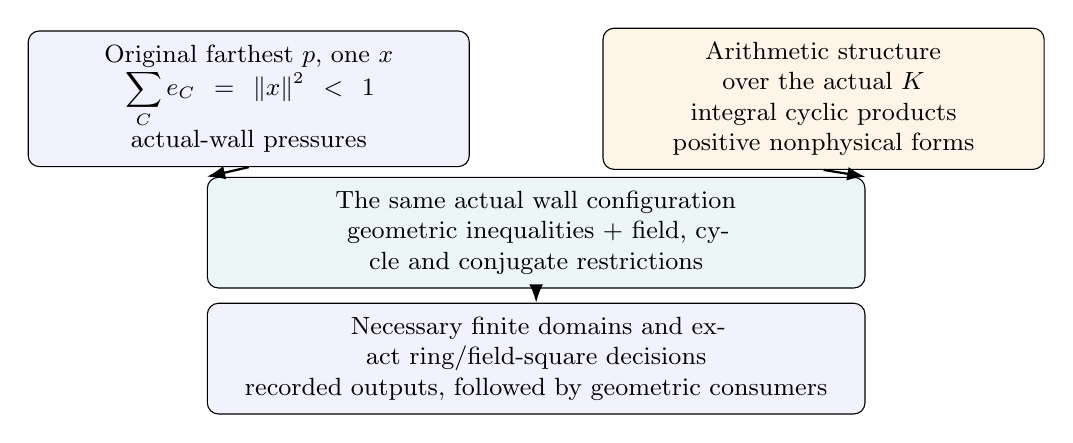
\begin{tikzpicture}[font=\small,>=Latex,
 box/.style={draw,rounded corners,align=center,minimum height=1.05cm,
 inner sep=5pt}]
 \node[box,text width=5.25cm,fill=blue!5] (geometry) at (3.0,3.35)
   {Original farthest \(p\), one \(x\)\\
    \(\displaystyle\sum_C e_C=\|x\|^2<1\)\\actual-wall pressures};
 \node[box,text width=5.25cm,fill=orange!9] (arithmetic) at (10.3,3.35)
   {Arithmetic structure over the actual \(K\)\\
    integral cyclic products\\positive nonphysical forms};
 \node[box,text width=8.0cm,fill=teal!7] (domain) at (6.65,1.65)
   {The same actual wall configuration\\
    geometric inequalities \(+\) field, cycle and conjugate restrictions};
 \node[box,text width=8.0cm,fill=blue!5] (consumer) at (6.65,.05)
   {Necessary finite domains and exact ring/field-square decisions\\
    recorded outputs, followed by geometric consumers};
 \draw[->,thick] (geometry.south)--(domain.north west);
 \draw[->,thick] (arithmetic.south)--(domain.north east);
 \draw[->,thick] (domain)--(consumer);
\end{tikzpicture}
\caption{Arithmetic restrictions on the wall parameters. The finite
algebraic domains and their outputs are given in
Proposition~\ref{arith:prop:pair-output} and Section~\ref{arith:sec:algorithms}.}
\label{arith:fig:ill20261026:a15:filter}
\end{figure}
% END ILLUSTRATION_20261026_A15_FILTER
\section{The complete rank-seventeen reduction}\label{arith:sec:seventeen}

Write $T_2=I_2(m)$, $m\ge3$, for an ordinary irreducible dihedral;
$T_3=A_3,B_3,H_3$ and $T_4=A_4,B_4,D_4,F_4,H_4$ unless a stated
field restriction removes a type. Put $\varphi=(1+\sqrt5)/2$.
Ordinary nonshort $A_1$ costs
 $>1/10$, ordinary $T_2>1/7$, $T_3>1/4$, $T_4>2/7$.
A total-rank-three forest need not cost $>1/4$; its ordinary bound
is $>17/70$.

The exceptions retain actual-wall meanings. Type $I$ is an isolated
short rank-one opposite
 \[
 c_I=\sqrt h\,p-\sqrt{1+h}\,e,\qquad0<h<1/2.
\]
Type $J$ couples two rank-one directions with joint energy $>.34$.
The typed rank-two defects are $N_7$, old $A_2$/new isolated-seven,
and $O_7$, old $I_2(7)$/new isolated-three. Each costs $>.09$;
they cannot coexist with one another or the short $I/J$ alternatives.
A bare old seven is not a typed defect.
These are the complete small-component alternatives of Proposition~\ref{arith:prop:f17}.
Their geometric compatibility proof uses the native gap between
distinct actual walls, not merely the abstract old forest.

\subsection{Shared costs and arithmetic prefix seals}\label{arith:subsec:shared-seals}

We specify the component inputs before carrying out either rank count.
The ordinary geometric rates are the component theorems of the general
compact companion, applied to whole orthogonal components at the same
original vertex:
\[
\begin{array}{c|c@{\qquad}c|c}
A_1&1/10&T_2&1/7\\
A_2&319/2000&A_3&1/4\\
B_3,H_3&2/7&A_4&2/7\\
H_4&11/36&B_4,D_4,F_4&1/3\\
A_5&3/8&D_5&5/14\\
B_5&3/7&A_6,B_6,D_6&3/7\\
B_7,D_7&1/2&B_8,D_8&4/7\\
E_6&9/20&E_7&5/9\\
E_8&2/3&&
\end{array}
\]
Every entry is a strict lower bound. In particular every ordinary
component outside $A_r$, $r\ge7$, and $B_r,D_r$, $r\ge9$, costs
more than its rank divided by fourteen. The universal large-component
rates used here are $A_r>1/2$ for $r\ge7$, $A_r>4/7$ for $r\ge8$,
$A_r>5/7$ for $r\ge13$, and $B_r,D_r>9/14$ for $r\ge9$.
These are geometric companion inputs, not assertions that a higher-rank
whole-diagram exclusion holds at a smaller rank. The stronger $B_3,H_3$
rate is needed only for the rank sixteen count; the rank seventeen count uses $1/4$.

The actual short-$I$ wall gives parameters $u,t$ with
 \begin{equation}\label{arith:eq:Ibarrier}
 e_I\ge u^2,\quad0<u<1/3,\quad
 (1-u^2)(1-t^2)=8ut,\quad t+3u/2>.767.
\end{equation}
Every normalized old dual direction outside $I$ has projection at
least $t$. Its squared-time parameter $h$ also gives the following
geometric alternative: at $h\le1/5$ all these squared projections are
at least $1/5$; at $h>1/5$, $e_I>3/70$.
These are the companion's actual opposite-wall barrier, with no
arithmetic hypothesis. We record the needed joint consequences here
to make their accounting explicit.

\begin{lemma}\label{arith:lem:Ijoint}
For ordinary irreducible $T_j$ the following bounds hold, each counting
 $I$ once:
\[
 e_{I+T_2}>.21,\qquad e_{I+T_3}>2/7,\qquad
 e_{I+T_4}>23/70,\qquad e_{I+A_1}>.20204,
 \qquad e_{I+2A_1}>.29.
\]
\end{lemma}
\begin{proof}
For $T_2$ use $e_{T_2}>1/7$ and $e_{T_2}\ge t^2$.
If $u\ge519/2000$, then $u^2+1/7>.21$.
Below that point $u^2+(.767-1.5u)^2$ is decreasing and has
endpoint value $.2100353125>.21$.

For $T_3$, its two endpoint correlations are $1/3$, $1/\sqrt3$
and $\rho$ with $\rho^2=(3\varphi+2)/(3\varphi+6)<16/25$,
respectively. Cauchy on the sum of the two unit directions gives
 $e_{T_3}>(10/9)t^2$, as well as $e_{T_3}>1/4$.
At $u\ge.19$ use $u^2+1/4>2/7$; below it the decreasing
quadratic $u^2+(10/9)(.767-1.5u)^2$ is at least
 $132407/450000>2/7$.

For $A_4$, the low-$h$ direction cover costs more than $1/3$;
the high-$h$ case gives $3/70+2/7=23/70$, strictly exceeded.
The $B_4,D_4,F_4$ rates already exceed $1/3$.
For $H_4$ we need $t+2u>6/7$. Substituting $6/7-2u$ for $t$
in the left-minus-right side of the identity in
\eqref{arith:eq:Ibarrier}, and multiplying by $49$, gives
 \[
13-168u+575u^2-168u^3+196u^4.
\]
With $v=u-.15$ this is
 $.269725-4.194v+525.86v^2-50.4v^3+196v^4$.
For $-3/20<v<11/60$ it is at least
 $.269725-4.194v+516.62v^2>0$, the last quadratic having
negative discriminant. The original identity decreases in $t$,
proving the barrier. At $u\ge19/125$, $u^2+11/36>23/70$;
below it the decreasing quadratic $u^2+(6/7-2u)^2$ is at least
 $50389/153125>23/70$.

For $I+A_1$, put $f(s)=(\sqrt{1+s}-1)/(\sqrt{1+s}+1)$.
The actual edge barrier gives half-tangent squares
 $q=f(h)$ and at least $r=f(1/(4h))$ on the other component.
Writing $P=\sqrt{qr}$, inversion gives
 $q+r=1+P^2-8P$, while AM--GM gives $q+r\ge2P$.
As $0<P<1$, this implies $P\le q_0=5-2\sqrt6$ and
 \[
 q+r-2q_0=(q_0-P)(8-P-q_0)\ge0.
\]
Thus $e_I+e_{A_1}\ge2q_0>.20204$; the rational seal is
 $2.44949^2>6$.
Finally, for two ordinary $A_1$ components, at $u\ge.3$ use
 $u^2+.2\ge.29$, strictly exceeded. Below it use
 $q(u)=u^2+2(.767-1.5u)^2$; then
 \[
q(u)-q(.3)=(.3-u)(2.952-5.5u)\ge0,
\qquad q(.3)=.290978>.29.
\]
Each calculation estimates one joint sum of orthogonal whole-component
energies; no endpoint has been charged a second copy of $I$.
\end{proof}

\begin{lemma}[Propagation from the actual old-seven defect]
\label{arith:lem:O7propagation}
Suppose a whole $I_2(7)$ component has an actual opposite supported
only there, with a native-three contact at one node and zero contact
at the other. Every other whole rank-one component has energy
 $>2/15$, and every other whole irreducible rank-two component has
energy $>1/5$. This lemma is geometric and allows arbitrary finite
spectators.
\end{lemma}
\begin{proof}
Put $d_7=\csc^2(\pi/7)$. The typed wall is
 $c_D=\sqrt{h_D}p-v_D$, with
 $h_D=d_7/4-1\in(0,1/3)$.
Let $c=\sqrt h\,p-v$ close an actual edge of another component.
Its finite endpoint retains the whole old $I_2(7)$.
A positive contact there contributes at least $d_7/4>1$ to the
white Schur cost, impossible. Thus $v$ has zero projection to
that whole component, and $c$ is distinct from $c_D$.
The native actual-wall gap gives
 \begin{equation}\label{arith:eq:O7height}
 (c_D,c)=-\sqrt{h_Dh}\le-1/2,\qquad h>3/4 .
\end{equation}
This proves the height bound for every opposite outside the defect,
without assuming an isolated profile for those other walls.
In a rank-one direction its spatial derivative is at most
 $\sqrt{1+h}$, so $\sinh^2L\ge h>3/4$. Hence its half-tangent
square is greater than $(11-4\sqrt7)/3>2/15$.

Suppose a whole $T=I_2(m)$, $m\ge3$, instead has energy $e\le1/5$.
Its normalized duals have correlation $k=\cos(\pi/m)$.
Write $s_i=x_T\cdot u_i$ and $F(s)=2s/(1+s^2)$.
For $m\ge4$, distinct actual opposites would require
 \[
 k\le F(s_1)F(s_2)\le F(\sqrt{1/5})^2
   =5/9<1/\sqrt2\le k,
\]
impossible. For $m=3$, Cauchy gives $(s_1+s_2)^2\le3/5$,
and concavity of $\log F$ gives the incompatible bound
 $1/2\le F(s_1)F(s_2)\le240/529<1/2$.
Therefore one actual wall closes both directions. Both lengths have
 \begin{equation}\label{arith:eq:O7length}
 \cosh L_i\le(1+1/5)/(1-1/5)=3/2 .
\end{equation}

Let $b,g\ge0$ be its contacts in $T$ and $Q$ its entire foreign
Schur cost. With $d=(1-k^2)^{-1}$, the finite endpoints give
 \[
\begin{gathered}
 Q+b^2<1,\quad Q+g^2<1,\qquad
 h=d(b^2+2kbg+g^2)+Q-1>3/4,\\
 C_b^2=\frac{d(b+kg)^2}{1-Q-g^2},\qquad
 C_g^2=\frac{d(g+kb)^2}{1-Q-b^2}.
\end{gathered}
\]
Every positive $b,g$ is consequently a finite native cosine.
At least one is positive. A positive whole foreign contribution
costs at least $1/4$, so $Q=0$ or $Q\ge1/4$.

For a single contact, say $b=\beta>0,g=0$,
$C_g^2=1+h/(1-Q-\beta^2)$.
Equations~\eqref{arith:eq:O7height}--\eqref{arith:eq:O7length} imply
 $Q+\beta^2<2/5$; hence $Q=0$ and the native gap forces $\beta=1/2$.
Then $h=d/4-1>3/4$ gives $d>7$ and $m\ge9$,
since $d_8=4+2\sqrt2<7$.
But $\sin t<t$ and $\pi^2<10$ give $d>81/10>31/4$,
so $C_g^2=(d-1)/3>9/4$, a contradiction.

If both contacts are positive and $Q>0$, let $g$ be the larger.
When $g\ge1/\sqrt2$,
$C_b^2\ge(4/3)(1+1/\sqrt2)^2>9/4$.
Otherwise $b=g=1/2$. At old label three, $h=Q<3/4$;
at old label at least four,
$C_b^2\ge(1+k)/(2(1-k))>5/2$.
Both are impossible.

It remains $Q=0$. If the larger contact has label at least five,
then $g>\!4/5$, $b\ge1/2$, $k\ge1/2$, $d\ge4/3$ give
 $C_b^2>3$. If both contacts have label four,
$C_b^2=(1+k)/(1-k)\ge3$.
The remaining finite contact pairs are $(3,4)$ and $(3,3)$.
For $(3,4)$, old label at least four gives $C_b\ge2$;
old label three gives $h=\sqrt2/3<3/4$.
For $(3,3)$, old label at least five gives
 $C_b^2=(1+k)/(3(1-k))>3$;
old labels three and four give $h=0,1/\sqrt2<3/4$.
Every contact and foreign case contradicts
\eqref{arith:eq:O7height} or \eqref{arith:eq:O7length}.
Thus $e_T>1/5$, completing both conclusions.
\end{proof}

Both typed defects force the actual field $K_7$. Their three actual
roots form the indefinite $(7,3,2)$ principal. Odd bonds permit a
square-two normalization over $K_7$; an extra embedding fixing $K_7$
would preserve that indefinite principal. Hence actual-field descent
gives $K=K_7$. In particular $H_3,H_4$ cannot occur beside a typed
defect, since their five-bond would put $\sqrt5$ in $K_7$.
For $N_7$ every other normalized dual has squared projection $>1/5$.
For $O_7$, Lemma~\ref{arith:lem:O7propagation} gives every other $A_1$
cost $>2/15$ and every other ordinary irreducible $T_2$ cost $>1/5$.
The hypothesis is the actual isolated-three wall, not the old label
seven alone.

\begin{lemma}[Literal arithmetic helpers]\label{arith:lem:literal-helper}
At a classified long-prefix index $i\ge6$ of $B_r$ or $D_r$, an
actual far helper
 $v=\gamma\omega_i+\omega_1/2$ with
 $202/125<2\gamma<12/5$ is impossible. At a $D$ fork-helper site
with $r\ge9$, the corresponding profile
 $v=\gamma\omega_i+\omega_f/2$ can only have $2\gamma=\varphi$.
\end{lemma}
\begin{proof}
Normalize the connected long roots to square two over $K$.
The simple-three helper contact permits the same normalization of
the actual outside root; its path cycle makes $t=2\gamma$ integral.
The short $B$ root has square one, so the entire old Gram is rational.
All embeddings of $\mathbb Q(t)$ extend to $K$, and every nonphysical
one must give a strictly positive Schur complement.

For the far helper the raw inverse entries $i,1,1$ give
 $it_\sigma^2+2t_\sigma-1<0$.
At $i\ge6$ this forces $|t_\sigma|<.61$ and $t_\sigma<.28$.
Degree at least three would give a nonzero integral norm of magnitude
less than $(12/5)(.61)^2<1$. In degree two the integral trace is
strictly between $503/500$ and $67/25$, hence two; its norm
 $t(2-t)$ lies strictly between $-1$ and one, again impossible.
Degree one leaves $t=2$, an actual parallel pair with a future feasible
null sum, contrary to compactness.

For the fork helper the inverse entries $i,i/2,r/4$ give
 \[
 4it_\sigma(t_\sigma+1)+r<8,
 \qquad-1<t_\sigma<0.
\]
The integral nonzero element $t(t+1)$ has physical value $<204/25$
and other conjugates of magnitude at most $1/4$. Its norm excludes
degree at least three. In degree two the trace of $t$ is one or two.
Trace one gives $t<2$ and norm in $(-2,-.995456)$, hence norm $-1$
and $t=\varphi$. Trace two gives norm in $(-24/25,0)$, impossible.
The rational $t=2$ is again parallel. This proves both assertions
without identifying $\mathbb Q(t)$ with the full field in advance.
\end{proof}

\begin{lemma}[The mixed $B_2$ tail]\label{arith:lem:B2seal}
At a $B_r$ site $i=r-2\ge12$, the actual own-three/short-three
profile $v=(\omega_i+\omega_r)/2$ is impossible.
\end{lemma}
\begin{proof}
Normalize the old long roots to square two and the short root to
square one over $K$. The simple-three short contact normalizes the
outside root to square one; its own-three product is $-1/\sqrt2$.
Thus $\sqrt2\in K$. At an embedding reversing $\sqrt2$, while fixing
the rational old Gram, its Schur cost is
 \[
 i/2-i/\sqrt2+r/4=i(3-2\sqrt2)/4+1/2>1.
\]
At $i=12$ the last inequality follows from $\sqrt2<17/12$,
and it increases with $i$. This contradicts strict positivity.
\end{proof}

For later prefix counts put
 \[
 f_j=\sqrt j-.61/\sqrt2,\qquad
 E_J=f_5^2/5+\sum_{j=5}^{J-1}(\sqrt{j+1}-\sqrt j)^2.
\]
The generic geometric inventory in the companion applies to $B_r$
with $M=r-5\ge6$ and to $D_r$ with $M=r-6\ge6$, through
 $M+1$. Every weak index is the literal far helper just excluded.
Hence $6,\ldots,J$ are strong, with $J=r-4$ in $B$ and $J=r-5$
in $D$. If five is strong, positive concave interpolation gives $E_J$.
If it is weak, its actual point gives $x_1>.5965$, $S_6>2.01815$;
interpolation through $1,6,J$ gives
 \[
 L_J=.7600299945+\frac{(\sqrt J-\sqrt6)^2}{J-6}>E_J,
\]
with the quotient zero at $J=6$. This follows from the variance
comparison: $E_6<.7$, and at most ten increments in $[1/8,1/5]$
have variance sum at most $9/640$, less than the initial gain $>.06$.
The rational lower seals used below are
 \begin{equation}\label{arith:eq:prefixfloors}
\begin{gathered}
\begin{array}{c|rrrrr}
J&6&7&8&9&10\\\hline
E_J>&.69685&.73531&.76864&.79805&.82436
\end{array}\\[4pt]
\begin{array}{c|rrrrr}
J&11&12&13&14&15\\\hline
E_J>&.84816&.86989&.88989&.9084&.92564.
\end{array}
\end{gathered}
\end{equation}
These statements retain the precise rank hypotheses of the companion
inventory; the smaller terminal ranks are handled below, rather than
being silently inserted into its generic range.

\begin{proposition}[Necessary cover in rank seventeen]\label{arith:prop:f17}
The whole forest at the original farthest vertex of a compact
arithmetic $17$-polytope is one of Table~\ref{arith:tab:f17}.
\end{proposition}
The proof below starts at rank seventeen. The arithmetic baseline
component estimates used in its partition stage are $e_{A_{15}}>.79$,
$e_{A_{16}}>.83$, $e_{A_{17}}>6/7$, and, under either actual typed
defect, $e_{A_{12}}>.703101$, $e_{A_{14}}>.7897732$.
Section~\ref{arith:app:arithcoverinputs} derives all these inputs from the
stronger printed whole-component proofs, with arbitrary spectators.
They are not higher-rank exclusions.

\begin{table}[ht]\centering\small
\begin{tabular}{clp{8.4cm}}
\toprule Group&Component&Complete spectators\\\midrule
1&$A_{11}$&$I+(A_5\text{ or }D_5)$\\
2&$A_{11}$&$N_7/O_7$ plus $A_4,B_4,D_4,F_4$\\
3&$A_{12}$&$A_5,D_5,(A_4\text{ or }H_4)+A_1,T_3+T_2,2T_2+A_1$\\
4&$A_{12}$&$I+T_4,\ I+T_3+A_1,\ I+2T_2$\\
5&$A_{14}$&$T_3,\ T_2+A_1,\ I+T_2$\\
6&$A_{15}$&$T_2,\ 2A_1,\ I+A_1,\ N_7/O_7$\\
7&$A_{16}$&ordinary $A_1$ or actual $I$\\
8&$A_{17}$&none\\
9&$B_{15}$&$N_7/O_7$\\
10&$B_{16}$&actual $I$\\
11&$B_{17}$&none\\
12&$D_{15}$&$N_7/O_7$\\
13&$D_{16}$&ordinary $A_1$ or actual $I$\\
14&$D_{17}$&none\\\bottomrule
\end{tabular}
\caption{The remaining spherical forests. Unmarked components are ordinary.}\label{arith:tab:f17}
\end{table}

\begin{proof}[Proof of Proposition~\ref{arith:prop:f17}]
Call $A_r$, $r\ge7$, or $B_r,D_r$, $r\ge9$, dominant.
There is exactly one dominant. With none, discarding only the one
possible $I$ leaves cost $>16/14$; a typed defect gives
 $>.09+15/14$. Ordinary or $J$ accounting is stronger.
Two dominants each cost more than $1/2$.
The complete ordinary table includes $E,F,H$, so this step loses no
exceptional irreducible component.

An $A_7$ leaves ten spectator ranks and is impossible by the same
budget. At $A_8,A_9,A_{10}$, even discarding $I$ leaves at least
six ordinary ranks, giving $4/7+6/14=1$, strictly exceeded.
The typed and $J$ alternatives are stronger. Thus $11\le r\le17$.

For $A_{11}$, ordinary spectator rank six already costs $>3/7$.
With $I$, the complete ordinary rank-five partitions are
 $5$, $4+1$, $3+2$, $3+1+1$, $2+2+1$, $2+1+1+1$, $1^5$.
Only $A_5,D_5,(A_4\text{ or }H_4)+A_1,T_3+T_2,2T_2+A_1$
can initially fit below $3/7$. Lemma~\ref{arith:lem:Ijoint} removes
the last three by $23/70+.1=3/7$, $2/7+1/7=3/7$, and
 $.21+1/7+.1>3/7$. Hence group1 is complete.
With a typed defect, ordinary rank four initially leaves $T_4$ or
 $2T_2$; the other partitions cost at least $.35$, $12/35$ or $.4$
before the defect is added. Propagation makes each $T_2>.2$,
removing $2T_2$; actual-field descent removes $H_4$. This gives group2.

For $A_{12}$, the complete cheap ordinary rank-five list is exactly
that just displayed. Indeed $B_5>3/7$,
$B_4,D_4,F_4+A_1>13/30$,
$T_3+2A_1>.45$, $T_2+3A_1>31/70$, and $5A_1>.5$.
A $J$ pair plus three remaining ranks costs $>.34+3/14>3/7$.
These give group3. With $I$, the rank-four partitions are
 $T_4,T_3+A_1,2T_2,T_2+2A_1,4A_1$.
The last two cost $>.29+1/7>3/7$ and $>.29+.2>3/7$,
respectively, using $I+2A_1$ only once. Thus group4 is complete.
A typed defect would leave ordinary rank three and give
 $.703101+.09+17/70>1$, so none remains here.

For $A_{13}>5/7$, ordinary or $J$ rank four already costs $>2/7$.
With $I$, the remaining rank-three partitions are $T_3,T_2+A_1,3A_1$;
their joint costs exceed $2/7$ by Lemma~\ref{arith:lem:Ijoint} or by
the ordinary three-$A_1$ cost. A typed defect plus $T_2$ costs
 $>.09+.2>2/7$; two ordinary $A_1$ cost at least $4/15$ and
give an even stronger contradiction. No $A_{13}$ row remains.

At $A_{14}>5/7$, ordinary spectator rank three leaves $T_3$ or
 $T_2+A_1$; three $A_1$ and $J+A_1$ are too expensive.
With $I$, only $I+T_2$ remains since $I+2A_1>.29>2/7$.
A typed defect gives $.7897732+.09+2/15>1$.
These are exactly group5.
At $A_{15}>.79$, rank two leaves $T_2,2A_1,I+A_1$, or either
typed defect. A $J$ pair closes; the other bounds do not delete the
retained alternatives. At $A_{16}>.83$, its single rank can be
ordinary $A_1$ or actual $I$. At $A_{17}$ there are no spectators.
This proves groups6--8 without an endpoint or field-degree inference.

For $B,D$, the $9/14$ rate and spectator accounting give $r\ge12$:
at six spectator ranks even the $I$ debit leaves $5/14$;
a typed defect gives $4/14+.09$. The generic arithmetic prefix
has last strong knot $J=r-4$ in $B$, $r-5$ in $D$, within the
rank domains specified above. The weakest floors at $r=12,13,14$
are therefore $E_7,E_8,E_9$.
At twelve their possible rank-five remainders cost more than
 $23/70$, $.09+17/70$, or $5/14$, respectively.
At thirteen all rank-four remainders cost $>2/7$, or at least
 $.09+.2$ in a typed case.
At fourteen the cheapest rank-three possibilities are ordinary
 $>17/70$, $I+T_2>.21$, $I+2A_1>.29$, and
typed $>.09+2/15$. Each closes with its stated prefix floor.
Thus no $B,D$ component of ranks twelve through fourteen remains.

We must extend the short tails at their actual ranks before counting
the proper higher rows. For $14\le r\le17$, the $B_3$ finite list
has only the extra short-three $F_4$ role; it is sealed against foreign
contacts and is affine or directly strong. At the $B_2$ site $i=r-2$,
the extra own-three/short-three profile is excluded by
Lemma~\ref{arith:lem:B2seal}. Own zero, four, six and parallel retain
their affine or null principals; native own at least five is directly
strong. A bridge through the short endpoint is a full $B_r$ with
internal new root and admits no finite foreign arm. Its residual is
 $1/(2i)$ and its ratio at least
 $1/\sqrt{2i}+\sqrt i/2>100/61$ for $i\ge11$.
All the other classified weak roles are excluded by
Lemma~\ref{arith:lem:literal-helper}. Hence $6,\ldots,r-2$ are strong,
so $e_{B_r}>E_{r-2}$ in either initial-five branch.
At $B_{15}$, $E_{13}>.88989$ excludes ordinary $T_2,2A_1,J,I+A_1$,
leaving either typed defect. At $B_{16}$, $E_{14}>.9084$ excludes
ordinary $A_1$ and leaves actual $I$. Whole $B_{17}$ is retained.

For $D_{15}$ the spectator rank is exactly two, and every allowed
remainder costs $>.09$. Its bulk already gives strong $6,\ldots,10$.
The local $D_4,D_3$ lists at indices eleven and twelve retain only
an additional own-five/fork-three case. More explicitly, own zero,
three, four, six and parallel have the same affine or null principals;
middle-three, end-four and the sealed $H_4$ end-five are directly
strong. The full bridge is $D_{15}$; at $D_3$ the end-three bridge
is $A_{15}$ with both arms at least three, so no finite foreign arm
is possible. Its residual $1/8+1/(2i)\le1/6$ and numerator $>.75$
make it strong; its zero-own cycle is affine.
The remaining fork helper is golden by
Lemma~\ref{arith:lem:literal-helper}.

For that golden role the actual positive left $H_4$ projection has
 \[
 \alpha^2=\varphi+5/8>56/25,\quad
 \delta=(5-3\varphi)/8,\quad \sqrt\delta/\alpha<.091,
 \quad A^2=i\alpha^2-\kappa,
\]
where $\kappa=1/2$ at $D_4$, $5/8$ at $D_3$.
The positive correction is
 $\gamma(3n_i/2+n_{i-1}+n_{i-2}/2)$.
The finite projection is future and feasible against all original
walls; the correction alone is not used as a hyperbolic point.
Its displacement divided by $\alpha$ is flat one on the first
 $i-3$ coordinates, has square $<i$, and gives pressure
 $G>\sqrt{i-\kappa/\alpha^2}-.091$.
Pay weight $1/6$ at the previous strong knot $K=i-3$.
Both initial-five references have endpoint coefficient $>1/6$,
so a single pure-$D$ square gives
 \[
 e_D>E_K+(G-f_K)/3-(i-K)/36.
\]
The complete two-row computation is
 \[
\begin{array}{c|rrrr|c}
 &i&K&G>&f_K<&e_D>\\\hline
D_4&11&8&3.19&2.398&.9493\\
D_3&12&9&3.33&2.569&.9683.
\end{array}
\]
The radical seals are $3.281^2<11-25/112$ and
 $3.421^2<12-125/448$. The pure energies each exceed $.91$;
adding only the disjoint actual spectator energy $>.09$ excludes
both roles. Thus $6,\ldots,12$ are strong and
 $e_{D_{15}}>E_{12}>.86989$.
Ordinary $T_2,2A_1,J,I+A_1$ close; either typed defect is retained.
At $D_{16}$ its ordinary $A_1$ and actual $I$ are both retained,
and whole $D_{17}$ is retained. These are groups12--14.

Every partition, actual defect and permitted dominant rank has now
been considered. No root has been deleted from another ambient list,
and every sum concerns the same original vector.
\end{proof}

\begin{proposition}[The other rows in rank seventeen]\label{arith:prop:old17}
Every row of Table~\ref{arith:tab:f17} except group8 is impossible.
\end{proposition}
\begin{proof}
The complete dispatch in Section~\ref{arith:app:arithrankseventeenclosure}
excludes groups1--7 and9--14. Each entry refers to its printed actual-wall,
field and individual-payment proof. The shared algebraic census for
whole B17 and D17 has separate actual-domain inclusions and separate
original-vector consumers. Group8 is treated next.
\end{proof}

\begin{proposition}[Actual chain endpoints]\label{arith:prop:a17reduce}
If group8 occurs, both actual endpoint opposites are isolated within
 $A_{17}$. Their integral parameters $U,V$ generate the same actual
field and satisfy
 \begin{equation}\label{arith:eq:a17strip}
 36/17<U,V<3969/425,\qquad
 0<U^\sigma,V^\sigma<36/17\quad(\sigma\ne\mathrm{id}).
\end{equation}
The field is nongolden, has degree at most five, and at least one
endpoint is finite. In fact
 \[
 K\in\{\QQ(\sqrt2),\QQ(\sqrt3),K_7,K_9\};
\]
in the cubic fields a finite endpoint has label seven or eighteen,
respectively.
\end{proposition}
Appendix~\ref{arith:app:wholearithA17} proves the complete endpoint,
field and domain-inclusion sequence of Sections~\ref{arith:app:arithA17endpointlist} and~\ref{arith:app:arithA17goldenends}, Section~\ref{arith:app:arithA17degree}, Section~\ref{arith:app:arithA17anchors}.
It retains every finite-white and own case, including the golden
time-compatible exception.
One decisive step explains the simultaneous accounting.
The common body has squared norm $.9037838$. Both dotted cores
are paid at weight $.3$; the outer coefficients change from
 $.1382$ to $.0782$ and still fund every central foot.
On the entire $0<u<1$ interval the extra contribution is
 \[
 .6\{\sqrt{17/9-u}-\sqrt{u(1-u)}-.4174\}
 -.09(8/5-2u+u^2)>.04969.
\]
The complete circle bounds in Appendix~\ref{arith:app:arithA17anchors} give
 $.9037838+2(.04969)>1$ if both ends are dotted.
No unavailable strong-five floor is used.
The complete finite alphabet, including label30 before its conjugate
test, then gives the stated fields, rather than a prescribed field list.

In raw old-root normalization of square two, a cap has square $2U$
and time square $F(U)/18$, where $F(X)=X(17X-36)$.
The inverse endpoint entry is $1/18$. Every actual pair consequently
satisfies
 \begin{equation}\label{arith:eq:a17cycles}
 R=F(U)F(V)\in K^2,\qquad
 g=(UV-\sqrt R)/18\in\OK,\qquad L=g^2/(UV)\in\OK.
\end{equation}
The root is physically positive. Acuteness gives $g\le0$.
If $g\ne0$, nonphysical positive definiteness gives $0<L^\sigma<4$.
The branch $g=L=0$ is retained. Physical owns and mutual parameters
must be native or dotted; four would be a compactness-forbidden
parallel pair. The endpoints need not be equal.

\section{Finite propositions and their complete algorithms}\label{arith:sec:algorithms}

The computations check necessary algebraic domains. An empty domain
excludes an actual configuration after geometric inclusion has been
proved. A nonempty domain supplies necessary pairs, followed by a
separate geometric contradiction, not examples.

\subsection{Full quadratic integer rings}
For squarefree $d>1$ use $\omega=(1+\sqrt d)/2$ if
 $d\equiv1\pmod4$, otherwise $\omega=\sqrt d$.
Let $\Delta$ be the fundamental discriminant.
If $Y=a+b\omega$ generates $K$, $Y>Y'>0$, $Y<B$, then
 \[
 0<b\sqrt\Delta=Y-Y'<B.
\]
Thus $\Delta<B^2$, and $b$ and the strip-permitted integers $a$
have explicit finite bounds. Squarefree trial division and these
integer intervals cover the full maximal order.

Use rational pairs $a+b\sqrt d$. Integrality in the half basis means
 $2b,a-b\in\ZZ$; otherwise both coefficients are integral.
Signs use exact rational square comparisons.
For $b\ne0$, a field square requires norm $n^2$ with rational
 $n\ge0$ and one of
 \[
 x^2=(a+n)/2,\quad x^2=(a-n)/2
\]
a nonzero rational square. Set $y=b/(2x)$ and verify the full
square identity. Both signed norm branches are necessary and
sufficient. For $b=0$ test rational squares and $d$ times rational
squares, including zero. A square norm alone is insufficient.

The complete positive quadratic finite native alphabet is
 \[
 1,2,3,(3+\sqrt5)/2,(5+\sqrt5)/2,2+\sqrt2,2+\sqrt3.
\]
Indeed $\phi(m)\le4$ leaves $m=3,4,5,6,8,10,12$.
Zero is orthogonality, values above four are dotted, and each
radical value is retained only in its actual field.

\begin{proposition}[Recorded finite outputs]\label{arith:prop:pair-output}
At the indicated complete domains the exact outputs are as follows.
\begin{enumerate}
\item The quadratic $A_{17}$ domain
\eqref{arith:eq:a17strip}--\eqref{arith:eq:a17cycles} has no survivor.
There are 25 discriminants $\Delta<88$, 53 models and 159 ordered
pairs: 106 fail field-square membership, 52 long-cycle integrality
and one two-cycle integrality.
\item The two cubic $A_{17}$ finite-anchor domains have the nine
strip models of Table~\ref{arith:tab:cubic}, all failing a necessary test.
\item The quadratic domain
 \[
 4<U<11,\ 0<U'<2,\quad2<W<676/17,\ 0<W'<4/17,
\]
$K=\QQ(U)=\QQ(W)$,
\[
 g=UW-\sqrt{U(U-2)W(17W-4)},\quad
 g,\ L=g^2/(2UW)\in\OK,\quad0<L'<4,
\]
with physical native/dotted mutual parameter, has 36 fields
 $\Delta<121$ and 120 pairs. Its only survivors are
 \[
 \begin{array}{c|cc}
 K&U&W\\\hline
 \QQ(\sqrt{13})&(5+\sqrt{13})/2&11+3\sqrt{13}\\
 \QQ(\sqrt{17})&(7+\sqrt{17})/2&(21+5\sqrt{17})/2 .
 \end{array}
\]
\item The quadratic whole-$B_{16}$ domain
 \[
 2<U<12,\ 0<U'<2,\quad4<V<64,\ 0<V'<1/4,\quad UV/2\in\OK,
\]
\[
 k^2=\frac{(U-2)V}{4U(4V-1)},\quad k>0,\quad
 G=4Uk(4V-1)-UV,\quad L=G^2/(2UV),
\]
with $k\in K$, integral $G,L$, actual acuteness and
the following exact predicates, has 43 fields $\Delta<144$:
$G\ge0$; if $G=0$ then $L=L'=0$, whereas otherwise
 $0<L'<4$; and $U,L$ must belong to the native finite alphabet
of their actual field or be greater than four. In particular $L=4$
is excluded, and no continuous nonnative value below four is allowed.
The identity
 \[
 L+G=((15U-32)/2)V-2U+4
\]
is checked for the physical positive square root $k$.
The complete domain has
100 head models, 85 short models and 273 pairs.
Exactly 168 fail half-product integrality and 104 field-square
membership. The sole survivor is $U=5+2\sqrt6$, $V=10+4\sqrt6$.
\end{enumerate}
\end{proposition}

The quadratic algorithm generates all fields below the proved
discriminant bound, lists all strip-permitted integer coefficients,
and visits every ordered pair. It applies full field-square,
cycle-integrality, conjugate-positivity and native tests, recording
every rejection or survivor and complete totals.
For (i), $b\le4$ and the conjugate width $36/17$ requires
\emph{three} candidates
 $a=\lfloor-b\omega'\rfloor+1,+2,+3$.
There are at most 3600 pair tests before the strict strips.
For (iii), $b_U\le4$, $b_W\le17$, with two $a_U$ values
and at most one $a_W$ value: at most 4896 pairs.
For (iv), safe full boxes are
 $1\le a_U\le7$, $1\le b_U\le5$ and
 $1\le a_V\le32$, $1\le b_V\le28$.
These bounds prove termination. The full-ring strip proof gives
coverage and the exact tests justify every rejection.
The floors themselves are exact integer operations:
\[
 \lfloor-b\omega'\rfloor=
 \begin{cases}
 \operatorname{isqrt}(b^2d),&\omega=\sqrt d,\\
 (\operatorname{isqrt}(b^2d)-b)\mathbin{\mathrm{div}}2,
       &\omega=(1+\sqrt d)/2.
 \end{cases}
\]
Irrationality places $b\sqrt d$ strictly between consecutive integers,
which proves both formulas, including even $b$.
Trial square division through $\operatorname{isqrt}(d)$ detects
squarefree radicands exhaustively. Fundamental discriminants below the
proved bound require no larger radicand loop.

\subsection{The two cubic finite anchors}
Let $U$ be the largest root of
 \[
 P_7=X^3-5X^2+6X-1,\qquad P_{18}=X^3-6X^2+9X-3.
\]
The full integer rings are $\ZZ[U]$. Polynomial discriminants are
49 and 81. Translating the first by four gives Eisenstein at
seven; the second is Eisenstein at three.
At the only possible index prime, an element
 $(A+B\pi+C\pi^2)/p$ with a coefficient not divisible by $p$
has a unique least numerator valuation among the distinct fractional
parts $0,1/3,2/3$; division by $p$ makes it nonintegral.
Thus no denominator is missing, including at the wild prime three.
In the $P_7$ field the complete physical finite alphabet for the other
own and the mutual parameter is
 \[
 0,1,2,3,U,U^2-3U+3;
\]
in the $P_{18}$ field it is
 \[
 0,1,2,3,U,U^2-4U+4.
\]
The last entries are native fourteen and nine, respectively.
Indeed a finite label requires $\phi(m)/2$ to divide three, leaving
the rational labels and $7,9,14,18$. The two cubic fields have different
discriminants, and contain no quadratic subfield. The double-angle
identity gives the displayed polynomial expressions. Values greater
than four are dotted, four is forbidden parallel, and zero is retained.

Write $V=a+bU+cU^2$. Rational root brackets and Lagrange
interpolation of the three embedding values give the complete boxes
 \[
 \begin{array}{c|ccc|r}
 &a&b&c&\text{trials}\\\hline
 P_7&[-4,4]&[-9,9]&[-3,3]&1197\\
 P_{18}&[-6,6]&[-9,9]&[-2,2]&1235.
 \end{array}
\]
Here is the coefficient proof, before any enumeration. The three
roots, in increasing order, have disjoint rational brackets
 \[
 \begin{array}{c|ccc}
 P_7&(.19,.20)&(1.55,1.56)&(3.24,3.25)\\
 P_{18}&(.46,.47)&(1.65,1.66)&(3.87,3.88).
 \end{array}
\]
Multiplying the six endpoint values by $10^6$ gives respectively
 \[
\begin{split}
P_7:&\quad-33641,8000;\ 11375,-11584;\ -35776,15625,\\
P_{18}:&\quad-32264,8423;\ 7125,-19304;\ -70797,4672.
\end{split}
\]
The three sign changes exhaust the roots of each cubic. If $r_i$ is
one of them, the denominator in its Lagrange basis polynomial is
 $P'(r_i)=\prod_{j\ne i}(r_i-r_j)$. The bracket gaps give absolute
lower bounds, in physical, middle, small order,
\[
 (5.1072,2.268,4.104),\qquad(7.514,2.6078,4.012).
\]
Use $0<V_{\rm phys}<10$ and $0<V_i<9/4$ at the other roots.
The coefficient of $X^2$ in the interpolant is
 $\sum_iV_i/P'(r_i)$, that of $X$ is
 $-\sum_iV_i\sum_{j\ne i}r_j/P'(r_i)$, and the constant is
 $\sum_iV_i\prod_{j\ne i}r_j/P'(r_i)$. Triangle inequalities give
the following strict upper bounds on the three absolute terms:
\[
\begin{array}{c|ccc|c}
 &\text{physical}&\text{middle}&\text{small}&\text{sum below}\\\hline
P_7,c&2&1&.55&4\\
P_7,b&3.45&3.43&2.64&10\\
P_7,a&.62&.65&2.78&5\\
P_{18},c&1.34&.87&.57&3\\
P_{18},b&2.84&3.76&3.11&10\\
P_{18},a&1.04&1.58&3.62&7.
\end{array}
\]
Each entry follows by positive rational multiplication with the
denominator bound. For example the last constant terms are below
 $(9/4)3.25\cdot1.56/4.104<2.78$ and
 $(9/4)3.88\cdot1.66/4.012<3.62$.
Since $a,b,c$ are integers, these strict estimates give exactly the
safe boxes above. Negative coefficients have not been discarded, and
the boxes were obtained without looking at the successful strip models.

All field operations reduce modulo the cubic. If $s^2=R$ with $R$
integral, $s$ is integral. Rational $R$ is handled separately: an
odd-degree field contains its square root only if that root is
rational. Otherwise put
 \[
 A=\Tr R,\ B=((\Tr R)^2-\Tr(R^2))/2,\quad t=\Tr s,\ n=\N s.
\]
Try both signed integers $n$ with $n^2=\N R$ and all
 $-454\le t\le454$; require
 \[
 z=(t^2-A)/2\in\ZZ,\quad z^2-2nt=B,\qquad
 s=\frac{tR+n}{R+z}.
\]
The identity follows from the characteristic polynomial of $s$;
its denominator can vanish only for rational $R$. Verify $s^2=R$
and its physical positive sign.
The trace range is complete: the finite anchor has $U<4$ and
 $V<10$, so $F(U)<128$, $F(V)<1340$ and the physical root
has magnitude below $415$. Each other root magnitude is below
 $324/17<20$. Hence $|\Tr s|<455$.
Exact interval refinement terminates since no nonzero polynomial
of degree at most two vanishes at a cubic generator. The zero element
is first recognized by its three zero coefficients. For every other
element, evaluate its degree-at-most-two representative on each separate
isolating interval and bisect that interval until its sign is fixed.
The interval width tends to zero, proving that every sign decision
halts at the intended embedding.

\begin{table}[ht]\centering\small
\begin{tabular}{cll}
\toprule Field&$(a,b,c)$&First failure\\\midrule
$K_7$&$(0,1,0)$&long cycle not integral\\
&$(1,-2,1),(1,-1,1),(2,-2,1),(3,-5,2)$&not a field square\\
$K_9$&$(0,1,0)$&long cycle not integral\\
&$(1,-2,1),(2,-2,1),(3,-3,1)$&not a field square\\\bottomrule
\end{tabular}
\caption{All nine cubic strip models.}\label{arith:tab:cubic}
\end{table}
All 2432 triples are visited. The recorded first failures are
1287 below the physical lower bound, 919 above its upper bound,
217 nonphysical-strip failures, seven field-square failures and
two nonintegral long cycles. They sum to 2432.
The separate combination replays every trial with the same implementation.

\begin{corollary}\label{arith:cor:no17}
There is no compact arithmetic Coxeter polytope of dimension seventeen.
\end{corollary}
\begin{proof}
The complete cover and row exclusions leave whole $A_{17}$.
Its actual endpoint reduction gives the quadratic or cubic fields
above. Proposition~\ref{arith:prop:pair-output}(i) excludes the former.
In a cubic field designate a finite endpoint first, reversing chain
labels if necessary; this assumes no chamber symmetry.
Every other endpoint lies in the complete box of (ii), which has
no survivor. No farthest forest remains.
\end{proof}

\section{The complete rank-sixteen reduction}\label{arith:sec:sixteen}

The rank-sixteen classification in Proposition~\ref{arith:prop:f16}
starts with all finite components and
actual defect compatibility. Two dominant components each cost
 $>1/2$. With none, the largest allowed rank-one debit still leaves
ordinary cost $>15/14$; the typed case costs $>.09+14/14$.
The unique A dominant has rank at least ten and the B/D dominant
rank at least eleven. Their small classical tails are checked at
their actual ranks, including the direct $D_{11}$ boundary.
The $D_{14}$ weak-tail payments give pure energies $>.92531$
or $>.94697$ before the disjoint spectator cost $>.09$ is added.
Only then are the stronger tail floors used.

The conditioned $A_{11}>.652761$ component input used below is proved
independently of either forest cover in
Corollary~\ref{arith:cor:arithA11conditionedcover}. Its proof reconstructs the
no-helper reference directly; the weaker uniform $13/20$ theorem would
not imply that value.

\begin{proposition}[Necessary cover in rank sixteen]\label{arith:prop:f16}
The whole forest at the selected original farthest vertex is one of
Table~\ref{arith:tab:f16}.
\end{proposition}
\begin{longtable}{clp{8cm}}
\caption{Necessary groups in rank sixteen.}\label{arith:tab:f16}\\
\toprule Group&Component&Complete spectators\\\midrule\endfirsthead
\toprule Group&Component&Complete spectators\\\midrule\endhead
1&$A_{10}$&$I+(A_5\text{ or }D_5)$\\
2&$A_{10}$&$N_7/O_7$ plus $A_4,B_4,D_4,F_4$\\
3&$A_{11}$&$A_5,D_5,(A_4\text{ or }H_4)+A_1,A_3+T_2,2T_2+A_1$\\
4&$A_{11}$&$I+T_4$\\
5&$A_{11}$&$O_7+A_3$\\
6&$A_{12}$&$A_4,H_4$ or $2T_2$\\
7&$A_{12}$&$I+T_3$\\
8&$A_{12}$&$N_7/O_7$ plus $T_2$\\
9&$A_{13}$&$A_3,\ T_2+A_1,\ I+T_2,\ O_7+A_1$\\
10&$A_{14}$&$T_2,\ 2A_1,\ I+A_1,\ N_7/O_7$\\
11&$A_{15}$&ordinary $A_1$ or actual $I$\\
12&$A_{16}$&none\\
13&$B_{14}$&$N_7/O_7$\\
14&$B_{15}$&ordinary $A_1$ or actual $I$\\
15&$B_{16}$&none\\
16&$D_{13}$&$I+T_2$ or $O_7+A_1$\\
17&$D_{14}$&ordinary $I_2(m)$, $m\ge4$, or $N_7/O_7$\\
18&$D_{15}$&ordinary $A_1$ or actual $I$\\
19&$D_{16}$&none\\\bottomrule
\end{longtable}

\begin{proof}[Proof of Proposition~\ref{arith:prop:f16}]
We repeat the rank count from its beginning. If no dominant occurs,
the possible $I$ debit leaves fifteen ordinary ranks, costing $>15/14$;
a typed defect gives $>.09+14/14$. A $J$ pair is more expensive than
the two rank-over-fourteen baseline costs it replaces. Two dominants
again each cost $>1/2$. Thus there is exactly one.
For $A_7$ the nine remaining ranks are too expensive. For $A_8,A_9$,
even $I$ leaves at least six ordinary ranks, giving
 $4/7+6/14=1$, strictly exceeded; the typed cost is at least
 $4/7+5/14+.09>1$. Therefore $10\le r\le16$.
For $B,D$, the $9/14$ rate leaves at most five spectator ranks,
so $11\le r\le16$. All exceptional finite types were already
included in the ordinary table.

At $A_{10}$, ordinary or $J$ rank six closes with $4/7$.
With $I$, enumerate the seven rank-five partitions displayed in the
rank seventeen proof. In $4+1$ use $I+A_1>.20204$ plus $T_4>2/7$;
in $3+2$ use $I+T_3>2/7$ plus $T_2>1/7$; in $2+2+1$
use $I+A_1>.20204$ plus $2/7$. The more reducible partitions
are stronger. Only $I+A_5,I+D_5$ remain.
With a typed defect, the rank-four partitions are
 $T_4,T_3+A_1,2T_2,T_2+2A_1,4A_1$.
The propagated costs exclude all but $T_4$, and actual $K_7$
excludes $H_4$. These give groups1 and2.

At $A_{11}>4/7$, the complete ordinary rank-five list below the
remaining $3/7$ budget is
 \[
 A_5,D_5,(A_4\text{ or }H_4)+A_1,A_3+T_2,2T_2+A_1.
\]
The omitted $B_5$ costs $>3/7$;
$B_4,D_4,F_4+A_1>13/30$;
$B_3,H_3+T_2>3/7$; and the other three reducible partitions
have costs $>.45$, $31/70$ and $.5$. This is group3.
The $J$ cost $.34+17/70$ also closes.
For actual $I$ use the spectator-safe conditioned component estimate
 $e_{A_{11}}>.652761$. Of the five rank-four partitions only $T_4$
remains: $I+T_3+A_1$ costs $>2/7+.1$,
$I+2T_2>.21+1/7$, and the other reducible cases are stronger.
Both resulting sums with $.652761$ exceed one. Thus group4 retains
all five irreducible $T_4$ types.

Under a typed defect the same component floor $.652761$ holds.
At remaining ordinary rank three, $T_2+A_1>.2+2/15$ and
 $3A_1>2/5$ close. So do $B_3,H_3>2/7$; $H_3$ is also
incompatible with $K_7$. Only $A_3$ is possible. For $N_7$ its
two normalized endpoint duals have correlation $1/3$ and heights
 $>1/\sqrt5$. Cauchy on their sum gives
 \[
 e_{A_3}>\frac{4/5}{2+2/3}=3/10,
\]
which closes with $.652761+.09$. Thus only $O_7+A_3$ remains,
giving group5.

At $A_{12}$ use its spectator-safe floor $269/400=.6725$.
Ordinary rank four leaves only $A_4,H_4,2T_2$:
$B_4,D_4,F_4>1/3$, $T_3+A_1>.35$,
$T_2+2A_1>12/35$, and $4A_1>.4$.
The $J$ alternative is stronger. With $I$, rank three leaves only
 $I+T_3$, since $.6725+.20204+1/7>1$ and $3A_1$ is stronger.
Under a typed defect the component floor is $.703101$;
two ordinary $A_1$ cost $>4/15$ and close, whereas a single
 $T_2>.2$ gives only $.993101$ and is honestly retained.
These are groups6--8.

At $A_{13}>5/7$, ordinary $B_3,H_3$, three $A_1$, and $J+A_1$
close. The retained ordinary alternatives are $A_3,T_2+A_1$.
With $I$, only $I+T_2$ remains since $I+2A_1>.30204$.
With $N_7$, an $A_1>.2$ closes; with $O_7$, the weaker $2/15$
does not. This is group9. At $A_{14}>.76$, the rank-two list is
ordinary $T_2,2A_1,I+A_1$, or either typed defect; $J$ closes.
At $A_{15}$ its single spectator is ordinary $A_1$ or actual $I$;
whole $A_{16}$ has none. This gives groups10--12, with no endpoint
or field-degree conclusion smuggled into the cover.

We now check the smaller classical ranks. For $B_r$ and $D_r$ with
 $r\ge12$, the legal generic prefix and
Lemma~\ref{arith:lem:literal-helper} give strong $6,\ldots,r-4$ and
 $6,\ldots,r-5$, respectively. At $D_{11}$ the generic parameter
 $M=5$ is not allowed. Instead inspect its actual deletion sites five
and six: the retained pieces are $A_4+D_6$ and $A_5+D_5$.
The connected white rank eleven exceeds eight, so the ordinary bulk
bridge list still applies. Its $D_5,D_6$ fork-to-$E_6,E_7$ contacts
remain included and strong; the foreign-far bounds use only indices
five and six, within their geometric range $5\le i\le29$.
The left finite-five projection uses the first six long roots, all
present. Thus the only weak-five/six profile is again the literal
far-three helper, and Lemma~\ref{arith:lem:literal-helper} excludes weak six.
This proves strong six without applying the generic theorem outside
its rank hypotheses.

Both initial-five branches therefore give the floors
\eqref{arith:eq:prefixfloors}, beginning with $E_6$ at $D_{11}$.
At classical rank eleven the cheapest rank-five remainders cost
 $>23/70$, $.09+17/70$ or $5/14$, all closing with $.69685$.
At twelve all rank-four remainders cost $>2/7$; a typed defect plus
 $T_2$ costs $>.29$. These close with $E_7>.73531$.
At thirteen ordinary or $J$ rank three closes with $E_8>.76864$.
Only $I+T_2$ or $O_7+A_1$ can remain; $I+2A_1$ and $N_7+A_1$
are more expensive. In $B_{13}$ the better actual floor
 $E_9>.79805$ closes both retained cases. In $D_{13}$ they are
group16.

For $B_{14}$ the actual $B_3$ site is eleven and the $B_2$ site
twelve. The former's extra short-three extension is sealed $F_4$;
own zero is affine and positive own has residual $1/4$ and ratio
at least $1+1/\sqrt2$, hence is strong. At the latter the only extra
weak role is excluded by Lemma~\ref{arith:lem:B2seal}. Full bridges have
residual $1/(2i)$ and ratio
 $1/\sqrt{2i}+\sqrt i/2>100/61$; they admit no foreign arm at
their internal new root. The zero/four/six/null cases and the directly
strong native owns are those already listed in the rank seventeen proof.
Thus $6,\ldots,12$ are strong, giving $e_{B_{14}}>E_{12}>.86989$.
Ordinary $T_2$, two $A_1$, $I+A_1$ and $J$ close; either typed
defect is retained as group13. The same local sites at $B_{15},B_{16}$
give strong through $r-2$, but leave their stated groups14 and15.

For $D_{14}$ the spectator rank is two and always costs $>.09$.
Its bulk already gives strong $6,\ldots,9$ independently of the
new tail sites. At site ten the right $D_4$ has long-leaf-three and
fork-three extensions. Their scalars differ: the former has
 $\sigma=\gamma+1/2$; the latter has
 $\delta=1/2-Q$, $\sigma=\gamma+1/4$.
At site eleven, $D_3=A_3$ has middle-three, end-three, end-four and
end-five extensions. Middle-three and end-four are affine or directly
strong; the sealed $H_4$ end-five is strong even at own zero.
The end-three full bridge is $A_{14}$ with both arms at least three,
so admits no finite foreign arm. Its residual is at most $15/88$,
and its positive-own numerator $>.75$ makes it strong; own zero is
the affine cycle. Full fork bridges are $D_{14}$ and are similarly
sealed. All other positive foreign, isolated and finite-own roles are
the generic companion list at these actual local ranks.

The only extra weak cases are therefore the literal fork helpers;
Lemma~\ref{arith:lem:literal-helper} leaves their golden owns.
Use their actual positive $H_4$ projections with the same
 $\alpha,\delta,\kappa$ as in the rank seventeen proof. For $K=i-3$ the
previous strong knot has available coefficient $>1/6$ in both
initial-five branches. One pure-$D$ reference gives
 \[
 e_D>E_K+(G-f_K)/3-(i-K)/36.
\]
Here the complete new rows are
 \[
\begin{array}{c|rrrr|c}
 &i&K&G>&f_K<&e_D>\\\hline
D_4&10&7&3.035&2.215&.92531\\
D_3&11&8&3.183&2.398&.94697.
\end{array}
\]
The seals are $3.126^2<10-25/112$ and
 $3.274^2<11-125/448$. Each pure bound plus the disjoint actual
spectator cost $>.09$ exceeds one. Hence both weak roles are
impossible, and $6,\ldots,11$ are strong. This gives
 $e_{D_{14}}>E_{11}>.84816$.
Two $A_1$, $I+A_1$, and $J$ close. Ordinary $A_2$ also closes,
since $.84816+319/2000=1.00766$.
Precisely an ordinary $I_2(m)$, $m\ge4$, or either typed defect
remains as group17. At $D_{15}$ the single ordinary $A_1$ or
actual $I$ is retained, and whole $D_{16}$ has none.

All small types, ranks, integer partitions and actual defect choices
were included before this final table. In particular no rank seventeen forest
was decremented and no farthest property was transferred to a face.
\end{proof}

\subsection{A small component calculation}

\begin{lemma}\label{arith:lem:A3point26}
At the original farthest vertex of any compact Coxeter polytope,
a whole $A_3$ component has energy $>13/50$, with arbitrary finite
spectators. Arithmeticity is not needed.
\end{lemma}
\begin{proof}
The inverse unit Gram and normalized old duals are
 \[
 C=\begin{pmatrix}3/2&1&1/2\\1&2&1\\1/2&1&3/2\end{pmatrix},
 \qquad d_i=C_{ii},\quad u_i=\omega_i/\sqrt{d_i}.
\]
Suppose $e=\|x_{A_3}\|^2\le13/50$. Put
 $\tau_i=\tanh(L_i/2)\le x\cdot u_i$ and
 $H(t)=2t/(1+t^2)$. The logarithm of $H$ is concave on $(0,1)$:
its second derivative is $-1/t^2-2(1-t^2)/(1+t^2)^2<0$.
For a pair of normalized duals with correlation $k$, Cauchy gives
 $\tau_i+\tau_j\le\sqrt{2e(1+k)}$; hence
 \[
 \tanh L_i\tanh L_j
 \le H\bigl(\sqrt{e(1+k)/2}\bigr)^2.
\]
At an adjacent $A_3$ pair $k=1/\sqrt3$, the right side is at most
 $5200(1+k)/(113+13k)^2<k$.
The cleared positive difference is $(22876k-12662)/3>0$,
using $k>4/7$. The companion's actual distinct-opposite
tangent-product inequality requires the opposite inequality if the
two walls are distinct. Thus adjacent directions share their actual
opposite, and connectivity gives one wall $c$ closing all three edges.

The individual bound is
 \[
 \tanh^2L_i\le\frac{4e}{(1+e)^2}\le r:=2600/3969.
\]
Write $c=A p-v_A-v_S$, $h=A^2>0$,
$v_A=\sum\beta_i\omega_i$, and $\beta_i=-(c,n_i)\ge0$.
Put $q=\beta^TC\beta$, $Q=\|v_S\|^2$, so $h=q+Q-1$.
For $v_i=(C\beta)_i/\sqrt{d_i}>0$ we have
 \begin{equation}\label{arith:eq:A3smallheight}
 q-1\le h\le r\min_i v_i^2.
\end{equation}
The companion's reciprocal-shadow and orthogonal-opposite lemmas
say that every positive whole spectator contribution is at least
 $1/4$ and strictly below $h$. In particular $h<1/4$ forces $Q=0$.

Two adjacent positive $\beta_i$ would give, at the finite endpoint
of the third edge, a white triangle with all three contacts at least
 $1/2$. Its Gram is nonpositive, affine at equality, impossible.
Thus there are at most two contacts, and two can only be at endpoints.
For endpoint values $a,b>0$,
\[
q=\tfrac32(a^2+b^2)+ab,\qquad v_2^2=(a+b)^2/2.
\]
If both are $1/2$, the original principal is affine with a nonzero
future feasible null sum. Otherwise the native gap gives $a,b\ge1/2$
and one at least $1/\sqrt2$. Consequently
 \[
q-rv_2^2\ge\frac{3(3-r)}8+\frac{(1-r)\sqrt2}4
 =\frac{27921+2738\sqrt2}{31752}>1,
\]
using $\sqrt2>7/5$. This contradicts \eqref{arith:eq:A3smallheight}.
There is at least one contact, since each $v_i>0$.

For one endpoint contact $\beta$, $q=3\beta^2/2$ and
 $\min v_i^2=q/9$. Equation~\eqref{arith:eq:A3smallheight} gives
 \[
 q\le35721/33121,\quad \beta^2\le23814/33121<3/4,
 \quad h\le2600/33121<1/4.
\]
Only native three, four or five remains, and each has $q<1$.
For five use $\cos^2(\pi/5)<2/3$, following from $\sqrt5<7/3$.
Then $Q=0$ and $h=q-1<0$, impossible.

For one middle contact, $q=2\beta^2$, $\min v_i^2=q/3$.
Thus $q\le11907/9307$ and
 $\beta^2\le11907/18614<16/25<\cos^2(\pi/5)$.
Only native three or four remains, so first conclude $q\le1$,
and only then strengthen the height bound to
 $h\le r/3=2600/11907<1/4$.
Again $Q=0$ and $h=q-1\le0$ is impossible. All contact and
foreign-spectator alternatives have been exhausted.
\end{proof}

\begin{proposition}[All rows except whole $D_{16}$]\label{arith:prop:onlyd16}
Groups1--18 are impossible at that same selected original vertex.
\end{proposition}
\begin{proof}
Groups1--18 are excluded by the complete printed dispatch in
Section~\ref{arith:app:arithranksixteenclosure}. Its separate actual rank-one
branches exhaust the same opposite wall, including the boundary $h=1/2$.
Every overlapping endpoint/head/foot pressure is paid within its local
proof before disjoint whole-component costs are added. The universal
 $A_{12}>5/7$ estimate supplies both ordinary and typed consumers.
Only group19, whole $D_{16}$, remains for the next section.
\end{proof}

\section{The last actual diagram}\label{arith:sec:d16}

\begin{proposition}[Whole-$D_{16}$ reduction]\label{arith:prop:d16reduce}
If group19 occurs, the actual field is quadratic. The actual long
head and both genuine signed forks are isolated and dotted. There
are integral generators $U,F,G\in\OK$ satisfying
 \begin{equation}\label{arith:eq:d16strips}
 4<U<98/9,\quad0<U'<2,\qquad
 4<F,G<121/2,\quad0<F',G'<1/2,
\end{equation}
\begin{equation}\label{arith:eq:quarters}
 UF/4,\ UG/4,\ FG/4\in\OK.
\end{equation}
Their raw time squares are
 \begin{equation}\label{arith:eq:times}
 T_H=U(U-2),\qquad T_F=2F(2F-1),\qquad T_G=2G(2G-1),
\end{equation}
and every pair of time products is a square in $K$.
\end{proposition}

We give its field and endpoint reduction below, after specifying the
initial geometric inventory and two scalar estimates. The inventory
must be proved at actual rank sixteen; it is not supplied by a
higher-rank head theorem or by the dyadic calculation.

The original coordinates satisfy
 \[
 x_1>\cdots>x_{15}>|x_{16}|,\quad P_j=e_1+\cdots+e_j,\quad
 S_j=x\cdot P_j,\quad f_j=\sqrt j-.61/\sqrt2.
\]
The same reduction proves strong5 through 14 and one positive prefix
reference with
 \begin{equation}\label{arith:eq:reference}
 E_{14}>.9084,\quad b<.361,\quad
 \beta_5>.14,\quad\beta_{14}>.13,\quad f_{14}<3.311,
 \qquad S_6>2.01815.
\end{equation}
Here $b$ is its first-five mean. These coefficients are spent
individually below. The head raw root has square $2U$, spatial
part $Ue_1$; the fork raw roots have squares $2F,2G$ and spatial
parts $(F/2)(P_{15}+e_{16})$, $(G/2)(P_{15}-e_{16})$.
They remain two distinct directions even if $F=G$.

The remainder of this exclusion is given in full. No D16 census is
used. Every original cycle remains mandatory even when only necessary
consequences of it are needed.

\begin{lemma}[Initial whole-$D_{16}$ inventory]\label{arith:lem:D16initial}
At the same original whole-$D_{16}$ vertex, knots five through fourteen
are $.61$-strong, and the positive reference has
\eqref{arith:eq:reference}. The actual long head is isolated, with finite
own label at least seven or dotted own. Every actual fork has edge
cosh less than twelve and is either isolated dotted or has exactly
one simple-three contact at an endpoint of its retained $A_{15}$ path,
with positive own contact. Own zero and parallel fork roles are excluded.
If both forks are isolated, the actual field has degree two or three.
\end{lemma}

The proof below first establishes the actual-rank coarse bounds and
head isolation, then closes the late spine and fork inventories.
This order keeps every pressure available before it is spent.

\begin{lemma}[Two exact terminal estimates]\label{arith:lem:terminal-scalars}
For $0<u<1$, put
 \[
 H(u)=\frac{\sqrt{2-u}-\sqrt{u(1-u)}}{\sqrt2},\qquad
 R(u)=1-u+u^2/2.
\]
Then $.8H(u)-.16R(u)>.295$. Also a degree-three algebraic integer
with conjugates $A,a,b>0$, $a,b<1/2$ and norm eight has $A>42$.
\end{lemma}
\begin{proof}
For the first assertion let $c=.681$, $t=2-c^2=1.536239$.
The radical difference is positive, and $t-u^2>0$.
It suffices to prove
 \[
 P(u)=(t-u^2)^2-4u(1-u)(2-u)>0.
\]
With $r=u-.7$ the exact expansion is
 \[
P=r^2(r-.6)^2+3.107522r^2-.0094692r+.002616045121.
\]
The last three terms exceed $3r^2-.01|r|+.0026$.
As $.01|r|\le r^2+.000025$, this is positive.
Thus $H(u)>c/\sqrt2>.4815351$ on the entire interval.

Moreover $R$ decreases, and $H$ decreases on $(0,.65]$.
Below $1/2$ the derivative sign is immediate; between $1/2$ and
 $.65$ it follows from
 \[
 \frac{2u-1}{\sqrt{u(1-u)}}\le\frac{.3}{\sqrt{.2275}}
 <\frac1{\sqrt{1.5}}\le\frac1{\sqrt{2-u}},
\]
where $.09\cdot1.5<.2275$ proves the strict inequality.
The following rational radical seals give lower bounds for $H(v)$:
\[
\begin{array}{c|ccc}
v&\sqrt{2-v}>&\sqrt{v(1-v)}\le&H(v)>\\\hline
.25&1.3228&.4331&.62\\
.4&1.2649&.4899&.54\\
.5&1.2247&.5&.51\\
.55&1.2041&.4975&.499\\
.6&1.1832&.4899&.4902\\
.625&1.1726&.48413&.4867\\
.65&1.16189&.47697&.4842.
\end{array}
\]
Square the first two columns and use $\sqrt2<1.4143$ to obtain
each last entry. Taking $H$ at the right endpoint and $R$ at the
left endpoint gives the complete cover
 \[
\begin{array}{c|c@{\qquad}c|c}
(0,.25]&.336&[.25,.4]&.307\\
{}[.4,.5]&.2992&[.5,.55]&.2992\\
{}[.55,.6]&.29596&[.6,.625]&.29656\\
{}[.625,.65]&.29611&[.65,1)&.29542808.
\end{array}
\]
These are strict lower bounds for $.8H-.16R$; the last uses the
global radical bound and $R(.65)=.56125$. Every endpoint is covered.

For the second assertion suppose $A\le42$. Norm eight and
 $a,b<1/2$ give $A>32$ and integer trace $T\in\{33,\ldots,42\}$.
Its minimal polynomial is $X^3-TX^2+BX-8$, with integer $B$.
Since $A>T-1$, AM--GM gives
 \[
 B\ge2\sqrt{8A}+8/A>2\sqrt{8(T-1)}+8/T.
\]
Evaluating the polynomial at $1/2$, between both small roots and
the large root, gives $B<T/2+63/4$.
For even traces the largest permitted $B$, and the positive seal
 $32(T-1)-B^2$, are
 \[
\begin{array}{c|rrrrr}
T&34&36&38&40&42\\\hline
B_{\max}&32&33&34&35&36\\
32(T-1)-B_{\max}^2&32&31&28&23&16.
\end{array}
\]
They contradict the lower bound. At $T=33$, $B_{\max}=32$ and
the same lower bound is already strictly larger than $32$.
At odd traces $35,37,39$, the permitted maxima are $33,34,35$;
the exact integers
 \[
 32(T-1)T^2-(TB_{\max}-8)^2=17191,14588,8087
\]
are positive and give the same contradiction after squaring.
Only $T=41$ remains. The two bounds force $B=36$, but
 $X^3-41X^2+36X-8$ has discriminant $-2704$, incompatible with
three real conjugates. Therefore $A>42$.
\end{proof}

\begin{proof}[Proof of Lemma~\ref{arith:lem:D16initial}]
All coordinates, caps and comparisons in this proof use the original
whole-$D_{16}$ vertex. Define its unit-root dual vectors by
 \[
 \Omega_i=\sqrt2P_i\quad(1\le i\le14),\qquad
 \Omega_{15}=(P_{15}-e_{16})/\sqrt2,\quad
 \Omega_{16}=(P_{15}+e_{16})/\sqrt2,
 \qquad h_i=x\cdot\Omega_i.
\]
Thus both genuine signed fork directions are retained.

\paragraph{The coordinate bound before any terminal classification.}
The legal rank sixteen bulk and Lemma~\ref{arith:lem:literal-helper} already
give strong knots six through eleven. We first use only those knots.
The quantities $E_J$ are the explicit scalar sums defined above;
in particular the identity
 \[
 \Delta:=E_{11}-E_6
   =\sum_{j=6}^{10}(\sqrt{j+1}-\sqrt j)^2>.15106
\]
is an analytic inequality, not an assertion that the actual vector
already pays the strong-five reference.
Here $E_{11}>.84816$ and
 \[
 E_6=12.03721-.122\sqrt{10}-2\sqrt{30}<.6971;
\]
the rational seals $\sqrt{10}>3.16227$ and $\sqrt{30}>5.47722$
prove the latter bound.

If $x_1\ge.714$, use the positive reference through
 $(1,.714),(6,2.01815)$ and then $f_7,\ldots,f_{11}$.
Its initial slopes are $.714,.26083$, followed by a smaller
positive slope and the ordinary decreasing increments. The first
increment after six is larger than $\sqrt7-\sqrt6$, because
 $f_6>2.01815$. Its square is therefore greater than
 \[
 .714^2+1.30415^2/5+\Delta>1.0010174445,
\]
contrary to $\|x\|^2<1$. Thus $x_1<.714$.
Actual head comparison then gives $C_H<77/25$, since
 $26/51>.714^2$. Neither the coordinate nor the head bound has
used strong five, a weak-five coordinate floor, or a head type.

\paragraph{The literal weak-five seal.}
At index five the generic finite-white list is the pure far helper
 $c=Ap-\gamma\Omega_5-\Omega_1/2$ if the knot is weak.
The first-six roots are genuine long roots, and the raw inverse
entries are $5,1,1$. Thus $q=2\gamma$ is integral,
$202/125<q<12/5$, and every other conjugate satisfies
 \[
 5q_\sigma^2+2q_\sigma-1<0,\qquad -.69<q_\sigma<.29.
\]
Degree at least four has nonzero norm $<2.4(.69)^3<1$.
In degree three the norm is a unit. A positive small conjugate would
give magnitude $<2.4(.29)(.69)<1$; both are therefore negative,
say $-a,-b$, with $ab=1/q$ and $a,b<.69$.
Then $q>1/(.69)^2$ and the integer trace lies strictly between
zero and two, hence is one. Thus $a+b=q-1<1.38$, $q<2.38$,
and the second integer coefficient $1/q-q(q-1)$ lies in $(-3,0)$.
The two cubics have discriminants $-44,-31$, impossible.
In degree two the trace is one or two. Trace two gives norm in
 $(-.96,.621)$; trace one also forces $q<1.69$, leaving only norm
 $-1$ and $q=\varphi$. The rational $q=2$ is parallel.
The actual connected principal is indefinite over
 $\mathbb Q(\varphi)$, so a weak five forces the actual field to be
exactly that field.

It also contradicts the coordinate bound already proved.
Here the selected old roots are $n_5,n_1,n_2$. Their correction
 $w=\gamma n_5+(2n_1+n_2)/3$ has positive coefficients and
 $w^2=\gamma^2+1/3$; the full selected diagram, including $c$,
is $H_4$. Thus $1-w^2=(5-3\varphi)/12$.
The positive actual left-$H_4$ projection gives
 \[
 x\cdot\{\gamma(\Omega_4+\Omega_6)/2+\Omega_3/6\}
 \ge \frac{A}{1+\sqrt{\delta/(A^2+\delta)}},
\quad
 A^2=(4+7\varphi)/2,\quad \delta=(5-3\varphi)/12.
\]
All coefficients in the finite projection are positive, so every
unselected original wall remains feasible. Long-arm concavity gives
 $h_4+h_6\le2h_5$ and $h_3\le3h_1$.
Weakness of five therefore forces
 $x_1>\sqrt2\{A-\sqrt\delta-\gamma(\sqrt{10}-.61)\}>.8$.
For a rational seal use $A>2.768$, $\sqrt\delta<.115$,
$\gamma<.81$, $\sqrt{10}<3.163$, and $\sqrt2>1.4$.
This contradicts $x_1<.714$. Consequently five is strong
before any head case is excluded.

\paragraph{The coarse fork bound after strong five.}
Knots five through eleven are now strong. Take their positive concave
reference through $f_5,\ldots,f_{11}$, with squared norm
 $E_{11}>.84816$, endpoint $f_{11}<2.886$ and available $P_{11}$
coefficient $\sqrt{11}-\sqrt{10}>.15$.
For either actual fork put $T_s=x\cdot(P_{15}+s e_{16})$.
The single tail graft $.15(P_{15}+s e_{16}-P_{11})$ has residual
square five and zero cross with that reference. Hence
 \[
 \|x\|^2>.84816+.3(T_s-2.886)-.1125.
\]
If its edge cosh were at least seventeen, then
 $T_s\ge4\sqrt{8/9}>3.77$, giving $1.00086>1$.
Thus both actual fork coshes are below seventeen.
This uses the strong-five reference only after its hypothesis has
been proved, with no head or fork classification assumed.

\paragraph{The exact head and fork white lists.}
Releasing the long root $n_1$ retains whole $D_{15}$. Finite
classification allows only an isolated new head or a simple-three
contact at its long leaf $n_2$. A fork attachment would require
a large exceptional diagram, an internal contact a second fork,
and two contacts a cycle; weighted alternatives are not finite.
For an isolated head,
$c_H=A_Hp-\gamma_H\Omega_1$ and $A_H^2=2\gamma_H^2-1$.
Own zero, three and four have nonpositive time; own six has the
actual affine $6,3$ chain, and parallel has the positive null
 $c_H+n_1$. The remaining owns are five, finite at least seven,
or dotted. With $U_H=4\gamma_H^2$,
\[
 K=\mathbb Q(U_H),\quad 2<U_H<11858/625,\qquad
 0<(U_H)_\sigma<2.
\]
The reflection-defined raw cap has square $2U_H$, own product
 $-U_H$, spatial part $U_He_1$ and nonzero time. Its indefinite
principal with the rational old system proves actual-field descent
and all the stated nonphysical inequalities.

For a nonisolated head write
 \[
 c_H=A_Hp-\gamma_H\Omega_1-\Omega_2/2,\qquad
 t_H=2\gamma_H,\quad A_H^2=t_H(t_H+2)/2,\quad C_H=t_H+1.
\]
The helper permits square-two normalization; its old path cycle
makes $t_H$ integral and gives $K=\mathbb Q(t_H)$.
Strict nonphysical positivity gives $-2<(t_H)_\sigma<0$.
Own zero has zero time; own three is an actual affine triangle;
parallel is a feasible null.

For either fork $f$, with the other called $k$, deleting $f$
retains the actual $A_{15}$ path $n_1,\ldots,n_{14},n_k$.
The complete finite one-node extensions are isolation, endpoint
three, next-to-end three, or endpoint four. Two contacts make a
cycle, and no exceptional finite diagram contains this path.
There are no foreign components. For positive own put $t=2\gamma$
at a white-three contact, $a=2\sqrt2\gamma$ at white four.
The following table gives UNIT time squares. For a white-three cap
the helper permits a raw $K$-root of norm two and time square $2A^2$.
For an isolated fork the reflection-defined raw norm is $2U_f$ and
its time square is $2U_f(2U_f-1)$. For a white-four cap use a raw
 $K$-root of norm four, with white product $-2$, own product $-a$
and time square $4A^2$. Indeed, if a $K$-root $r$ makes angle
 $\pi/4$ with an old raw root $\alpha$ of norm two, then
 $(r,\alpha)^2=(r,r)$; rescaling by $2/|(r,\alpha)|$ gives this
norm-four representative without assuming $\sqrt2\in K$.
\[
\begin{array}{c|c|c}
\text{white contact}&A^2&\text{actual edge cosh}\\\hline
\text{none}&2U_f-1,\ U_f=4\gamma^2&\sqrt{2U_f}\\
3\text{ at }n_1&(4t^2+t-1)/2&(8t+1)/\sqrt{17}\\
3\text{ at }n_2,n_{14}&(4t^2+jt+j-2)/2&4t+j/2,\ j=2,14\\
3\text{ at }n_k&(4t^2+7t+2)/2&(8t+7)/\sqrt{17}\\
4\text{ at }n_1&(2a^2+a)/2&4a+1\\
4\text{ at }n_k&(2a^2+7a+6)/2&4a+7 .
\end{array}
\]
The white-three normalization gives integral $t$ and $K=\mathbb Q(t)$.
White four gives integral $a$, integral $a^2/2$, and
 $K=\mathbb Q(a)$. These are original cycle statements.
An isolated fork has $K=\mathbb Q(U_f)$, all other
 $0<(U_f)_\sigma<1/2$, and raw time square $2U_f(2U_f-1)$.
These follow from its full indefinite old-system/cap principal.

Own zero has negative or zero time in the isolated, far-three,
far-next-three and far-four cases. Its remaining cases have the
following positive affine nulls:
\[
\begin{array}{c|l}
3\text{ at }n_{14}&c+n_{13}+n_f+n_k+2n_{14}\\
3\text{ at }n_k&2c+4n_k+6n_{14}+3n_f+5n_{13}
                  +4n_{12}+3n_{11}+2n_{10}+n_9\\
4\text{ at }n_k&\sqrt2c+2n_k+2n_{14}+n_f+n_{13}.
\end{array}
\]
Their products on the selected roots vanish. Their time is positive,
and every other original wall has nonpositive product term by term.
Parallel always gives $c+n_f$. This excludes own zero and parallel
without a head assumption.

\paragraph{Every nonisolated dotted head is impossible.}
Set $s=t_H+1=C_H$. Physically $3<s<77/25$; all its other
conjugates lie in $(-1,1)$. The nonzero integral element
 $s^2(s^2-1)$ has physical value $<81$ and other conjugate
magnitudes at most $1/4$, excluding degree at least five by its norm.
Degree one is excluded by Meyer. At degree two the integer trace is
three or four, giving norms $s(3-s)\in(-.2464,0)$ or
 $s(4-s)\in(2.8336,3)$, both impossible.

At degree four its absolute norm is one, so $s,s-1,s+1$ are units.
For the minimal polynomial $P=X^4-TX^3+BX^2-CX+D$,
$D=\pm1$, the real strips force $P(1)=-1$, $P(-1)=1$.
Hence $B=-1-D$, $C=1-T$.
For $D=1$,
$T=s-(s^2+s-1)/(s^3-s)$ lies strictly between two and three:
the fraction is below one and above $1/s>25/77$.
For $D=-1$,
$T=s+(s^2-s-1)/(s^3-s)$ lies strictly between three and four,
since its added fraction is in $(0,1/2)$. Both contradict integrality.

At degree three write $P=X^3-TX^2+BX-C$ and put
 $a=-P(1)>0$, $b=-P(-1)>0$. The integer norm satisfies
 $C^2ab<81/16<6$.
For $|C|=1$ the complete equal-parity pairs are
 $(1,1),(1,3),(3,1),(1,5),(5,1),(2,2)$;
for $|C|=2$ only $(1,1)$ remains.
Here $T=(a+b)/2-C$, $B=(b-a)/2-1$. The complete seals are
 \[
\begin{array}{r|c|c|l}
C&(a,b)&(T,B)&\text{seal}\\\hline
1&(1,1)&(0,-1)&P(3)=23\\
1&(1,3)&(1,0)&P(3)=17\\
1&(3,1)&(1,-2)&P(3)=11\\
1&(1,5)&(2,1)&P(3)=11\\
1&(5,1)&(2,-3)&\operatorname{disc}P=-23\\
1&(2,2)&(1,-1)&P(3)=14\\
-1&(1,1)&(2,-1)&P(3)=7\\
-1&(1,3)&(3,0)&P(3)=1\\
-1&(3,1)&(3,-2)&P(77/25)=-4.401088\\
-1&(1,5)&(4,1)&P(77/25)=-4.647488\\
-1&(5,1)&(4,-3)&P(77/25)=-16.967488\\
-1&(2,2)&(3,-1)&P(77/25)=-1.321088\\
2&(1,1)&(-1,-1)&P(3)=31\\
-2&(1,1)&(3,-1)&P(77/25)=-.321088 .
\end{array}
\]
Every displayed polynomial has derivative at least
 $3X^2-8X-3=(3X+1)(X-3)>0$ on the interval.
The sign seals or the negative discriminant exclude all fourteen.
This exhausts every dotted nonisolated head.

For finite own, the same norm bounds its actual degree by four.
The complete $\phi(2m)/2\le4$ list, after own three, is
 $m=4,5,6,7,8,9,10,12,15$.
At $7,8,10,12,15$ the embeddings with cosine multipliers
 $3,3,3,5,7$ give a positive nonphysical $t_H$, forbidden.
Only the finite heads $4,5,6,9$ remain.

\paragraph{The four finite nonisolated heads.}
Their parameters are
 $t_H=\sqrt2,\varphi,\sqrt3,2\cos(\pi/9)$ and their actual fields
are generated by these parameters. The first-five block of the
strong reference has mean $b<.361$. An actual floor $x_1>X$
permits rebuilding this block at fixed sum, gaining
 $\tfrac54(X-.361)^2$, with all its new slopes positive.
For $X=.643,.681,.695$ the remaining first-five slope exceeds
 $.27$, larger than the next ordinary slope $<.214$.
The original individual $P_{11}$ price still funds the signed tail.
The resulting complete fork bounds are
 \[
\begin{array}{c|c|c|c}
\text{head}&X&\text{forbidden fork }C\ge&\text{single norm lower}\\\hline
4&.643&7&1.001265\\
6&.681&6&1.01186\\
9&.695&6&1.023305 .
\end{array}
\]
The head squares satisfy respectively
 $x_1^2\ge\sqrt2-1$, $x_1^2\ge2\sqrt3-3$,
and $x_1^2\ge t_H/(t_H+2)$ with $t_H>1.87$.
The signed tail demands used are $>3.44$ at $C=7$ and $>3.38$
at $C=6$. For head five use $x_1>.668$ and the reference through
 $1,6,7,\ldots,11$, whose energy is
 $>.668^2+1.35015^2/5+.84816-.6971=.9618650045$.
At $C=49/8$, $T_s>3.39$, giving norm $>1.0005650045$.
Thus both fork coshes are below seven, $49/8$, six, six,
in the four respective cases.

No fork can be isolated in these cases. Its original cycle with the
nonisolated head gives, for integral $g,L$,
\[
 L+g(t_H+2)=(15t_H^2+28t_H-4)U_f/4-2t_H(t_H+2).
\]
At heads $5,6,9$, $t_H$ is a dyadic unit, forcing $U_f/4$ integral.
The positive norm bounds are $2401/4096$, $9/16$ and
 $(18/4)(1/8)^2$, each below one.
At head four normalize $v(\sqrt2)=1$. The displayed coefficient
has valuation two, so only $U_f/2$ is integral.
For $W=U_f/2\in\mathbb Z[\sqrt2]$, its strips are
 $W<49/4$, $0<W'<1/4$.
The radical coefficient is $1,\ldots,4$; only $W=3+2\sqrt2$
fits, giving $U_f=6+4\sqrt2$.
The original raw time product has square $1256+888\sqrt2$,
whose norm $448$ is nonsquare.

All remaining forks must be endpoint-three. Indeed near-next-three
and near-four have cosh at least eleven and greater than twelve.
Far-next-three has $t<3/2$, leaving only own three or own four.
Own three gives the actual fifteen-node all-three cycle
 $c,n_2,n_3,\ldots,n_{14},n_f,c$, where $f$ is the released fork.
The sum $c+n_2+\cdots+n_{14}+n_f$ is null: its positive all-ones
kernel annihilates every selected unit-Gram row. Its time is the
positive time of $c$, and acuteness makes its product with every
other original wall nonpositive. It is therefore a feasible ideal
ray of the whole chamber, contradicting compactness.
Own four has a conjugate violating its negative time strip.
Far-four has $a<3/2$, leaving only $a=\sqrt2$; its time numerator
 $2a^2+a$ is positive at $-\sqrt2$, also forbidden.
Own zero and parallel were already excluded.

For an endpoint-three cap its raw time square is
 $M_f(t)=4t^2+t-1$ far or $M_n(t)=4t^2+7t+2$ near,
with $K=\mathbb Q(t)$ and integral $t\ge1$.
Writing $z=t+1$ near, every nonphysical conjugate lies in
 $(-13/20,2/5)$ far or $(-2/5,13/20)$ near.
The full quadratic integer strips give
 \[
\begin{array}{c|c|c|c}
\text{head}&\text{far }t&\text{near }z&\text{time-product norms}\\\hline
4&1+\sqrt2&2+\sqrt2&72,\ 36\\
5&\varphi,\varphi^2&\varphi^2&5,\ 5,\ 95\\
6&\text{none}&\text{none}&
\end{array}
\]
At head four the physical bounds are $t<7/2$, $z<15/4$;
the positive integral radical coefficient is one, giving exactly
the displayed values. The square-norm near product
 $102+72\sqrt2$ would require rational square part $54$ or $48$.
At head five the physical parameters are below $10/3$; the
positive $\varphi$ coefficient is one, giving far integer coefficients
zero or one and near coefficient one. At head six the only strip
value is $2+\sqrt3$, above its respective bounds three and $13/4$.
No quadratic endpoint survives.

At head nine the actual degree is three. A far parameter has
 $1\le t<3$ and norm magnitude one; a positive small conjugate would
make the norm $<3(.4)(.65)<1$. Thus both are negative, $-a,-b$,
with $ab=1/t$, $a,b<.65$, so $t>400/169$.
Its integer trace is strictly greater than
 $400/169-1.3>1$ and less than $3-2/\sqrt3<2$, impossible.
Near, $2\le z<13/4$ has unit norm and both small conjugates positive,
since a negative one would give norm magnitude
 $<(13/4)(.4)(.65)<1$.
The integer trace is four. Then $z>2.7$ from $a+b<1.3$,
and $z<3$ because $z+2/\sqrt z>4$ at $z\ge3$.
The second integer coefficient $1/z+4z-z^2$ decreases on
 $(2.7,3)$ and lies strictly between $10/3$ and $10477/2700<4$.
This final contradiction excludes head nine. Both actual fork
opposites must exist, so the long head is isolated in every case.

\paragraph{White-four, next-three and finite isolated forks.}
The head is now isolated; its weak upper strip
 $U_H<11858/625$, $0<(U_H)_\sigma<2$ is retained.
A far white-four fork has integral $a$, integral $a^2/2$,
$a<4$, and every other $-.5<a_\sigma<0$.
Degree at least three has nonzero norm magnitude $<1$.
In degree two the magnitude is below two, but integrality of
 $a^2/2$ forces its norm even. Degree one is impossible.
Near, $z=a+2$ has $z<9/2$, all other $0<z_\sigma<1/2$,
and integral $z^2/2$. Degree at least four is excluded by norm.
At degree three its positive norm is one, incompatible with
integrality of $z^2/2$. At degree two that integrality forces norm
two. Then $z>4$ and its integer trace $z+2/z$ lies in $(9/2,5)$.
This excludes both white-four roles over every actual field.

For next-three at $n_2$, $1\le t<4$ and all other conjugates lie in
 $(-1/2,0)$. Degree at least three is excluded by norm; degree two
has norm $-1$ and trace two or three. Thus
 $t=1+\sqrt2$ or $(3+\sqrt{13})/2$.
For next-three at $n_{14}$ put $z=t+2$. Then $3\le z<9/2$ and
all other conjugates lie in $(0,1/2)$.
Degree at least four is excluded by norm. Degree three would have
norm one, $z>4$, and integer trace strictly between five and $11/2$.
At degree two norm two gives the same forbidden trace interval as
white four; norm one gives trace four, $z=2+\sqrt3$, $t=\sqrt3$.

For these three next-three parameters the actual head path cycle and
two-cycle give integral $g=-H\cdot C$, $L=g^2/U_H$, and
 \[
\begin{aligned}
L+g(t+2)&=(15t^2+4t-4)U_H/4-2M&&\text{far},\\
L+g(t+2)&=(15t^2+52t+44)U_H/4-2M&&\text{near}.
\end{aligned}
\]
Each listed $t$ is a dyadic unit, so $U_H/4$ is integral.
Writing $W=U_H/4$, its full strips are
 $W<11858/2500$, $0<W'<1/2$.
Use the full integral bases $1,\sqrt2$ and $1,\sqrt3$ in the
first and third fields, and $1,(1+\sqrt{13})/2$ in the second.
Writing $W=a+b\eta$ in the appropriate basis, the positive integer
coefficient $b$ is one in all three cases: $W-W'<11858/2500$,
whereas $b\ge2$ would give respectively at least
 $4\sqrt2$, $2\sqrt{13}$ or $4\sqrt3$, all larger than this bound.
In particular the
coefficient of $\sqrt{13}$ itself is $1/2$, not one.
The first two conjugate strips require
 $\sqrt2<a<\sqrt2+1/2$ or
 $(\sqrt{13}-1)/2<a<\sqrt{13}/2$, neither admitting an integer.
The last gives $a=2$, hence $W=2+\sqrt3$ and $U_H=8+4\sqrt3$.
Then $C_H=1+\sqrt3$, $x_1>.681$.
The near-next fork has $C=7+4\sqrt3>13$, hence $T_s>3.7$.
The reference through $1,6,7,\ldots,11$ has energy
 $>.681^2+1.33715^2/5+.84816-.6971=.9724150245$;
its legal signed tail graft gives
 $\|x\|^2>1.1041150245$. No next-three role survives.

For an isolated finite fork $F=4\cos^2(\pi/m)$, with actual degree
 $d$, its trace is $2d+\mu(m)$. The nonphysical strip $F_\sigma<1/2$
and physical $F<4$ give $3d<7-2\mu(m)$, hence $d\le2$.
The complete quadratic native list and the rational-field exclusion
leave only $F=\varphi^2$ or $2+\sqrt3$; native eight and ten have
conjugates above $1/2$. Both retained parameters are units.
The actual isolated head/fork cycle satisfies
 \[
 L+g=(15U_HF-32F-8U_H+16)/4,
\]
so $U_H/4$ is integral. The full integer strips give
 $U_H=4\varphi^2$ or $8+4\sqrt3$, respectively.
For the first, $x_1>.625$ and the positive left-$H_4$ projection
onto $c_f,n_f,n_{14},n_{13}$ gives
 \[
 V=P_{12}+(e_{13}+e_{14}+e_{15}-s e_{16})/2,\quad
 V^2=13,\quad x\cdot V>\sqrt{8\varphi}-(2\varphi-3)>3.36.
\]
Its old correction is
 $(\varphi/2)(3n_f/2+n_{14}+n_{13}/2)$, with positive coefficients
and residual $(5-3\varphi)/8$. Thus the finite projection is future
and feasible against every original wall.
The reference through $(1,.625),(6,2.01815)$ and the later knots
has energy $>.9298583845$. Its $.15P_{11}$ graft has residual
square two and gives norm $>1.0270583845$.
For native twelve the same original head gives $x_1>.681$.
Projection onto $c_f,n_f$ has divided displacement $P_{14}$ and
demand
 $\sqrt{8\sqrt3}-\sqrt2(2-\sqrt3)>3.34$.
Its positive correction is $\gamma_fn_f$ and residual
 $1-\gamma_f^2>0$. The reference energy is $>.9724150245$;
the $.15P_{11}$ graft has square three and gives norm
 $>1.0411150245$. Thus every isolated finite fork is excluded.
At this stage a fork is isolated dotted or endpoint-three.

\paragraph{Three head feet used by the remaining spine payments.}
For an isolated head write $c_H=A_Hp-\gamma_H\Omega_1$.
The actual first-three/four-root constructions give
 $x\cdot Z\ge H$, nonnegative $Z$ with sum one, and
 \[
\begin{array}{c|c|c|c}
\text{own}&Z&H&R=Z^2\\\hline
5&P_4/4&A_H/\sqrt2> .393&1/4\\
m\ge7&(1-u/2)(e_1+e_2)+(u-1)e_3&
{}[\sqrt{2-u}-\sqrt{7u-4-3u^2}]/\sqrt2&3-4u+3u^2/2\\
\text{dotted}&(1-u/2)e_1+(u/2)e_2&
H(u)&R(u).
\end{array}
\]
Here $u=\gamma_H^{-2}$; the dotted functions are those of
Lemma~\ref{arith:lem:terminal-scalars}.
The native-five row is the finite positive $H_4$ projection.
The finite row uses
 $\xi=c_H+n_1/\gamma_H+2(\gamma_H^{-1}-\gamma_H)n_2$.
Its square is $-(7-4\gamma_H^2-3/\gamma_H^2)<0$;
its products with $c_H,n_1$ vanish and that with $n_2$ is
 $(3-4\gamma_H^2)/(2\gamma_H)<0$.
The dotted row uses $\xi=c_H+n_1/\gamma_H$.
The time is positive in both cases, and all other original walls
have nonpositive products termwise.

For every finite $m\ge7$ and every dotted own,
\begin{equation}\label{arith:eq:D16headgain}
 .8H-.16R>.2893 .
\end{equation}
For seven, its cubic gives $.9009<\gamma_H<.901$.
Rational squares give $A_H>.7894$,
$\sqrt{7-4\gamma_H^2-3/\gamma_H^2}<.2395$,
$\gamma_H\sqrt2<1.2743$, hence $H>.4315$;
$1.2318<u<1.233$ gives $R<.349$ and the result $>.28936$.
For all finite $m\ge8$, $1<u\le4-2\sqrt2<1.172$.
Put $D=(u-1)(4-3u)$ and $a=.8/\sqrt2$.
The derivative of $.8H-.16R$ is
 \[
a\{-1/(2\sqrt{2-u})-(7-6u)/(2\sqrt D)\}+.64-.48u .
\]
It is negative on $(1,7/6]$: the first term is $<-.28$,
the second nonpositive, and the last at most $.16$.
On $[7/6,1.172)$, $\sqrt D>.284$, the positive second term is
 $<.032$, and the other terms are $<-.28+.08$.
The minimum is therefore at native eight, where
 $\sqrt{2-u}>.910$, $\sqrt D<.289$, $R<.373$, giving
 $H>.4388$ and $.8H-.16R>.29136$.
For dotted own Lemma~\ref{arith:lem:terminal-scalars} is stronger.
The graft $.4(Z-P_5/5)$ spends $.08<\beta_5$, is zero-sum
on the first-five flat block, and gives the single-reference gain
 $>.2893-.8(.361)+.032=.0325$.

\paragraph{The complete late $D_4,D_3$ inventories.}
At twelve the retained pieces are $A_{11}+D_4$, with right long
leaf thirteen, centre fourteen and the two genuine forks.
At thirteen they are $A_{12}+D_3$, the right $A_3$ having middle
fourteen and endpoints the forks. Finite classification gives:
left endpoint-three, next-three or endpoint-four; right $D_4$
three at any leaf; right $D_3$ middle-three or endpoint-three,
four or five; and bridges joining a left endpoint by three to a
right leaf or middle by three. The full bridges are $D_{16}$ or
 $A_{16}$. Other bridges have two forks, a weighted internal bond
or large unequal exceptional arms. Two contacts in one retained
component make a nonpositive cycle. These are all white cases.

With left contact at position $j$, the unit residual/ratio data are
 \[
\begin{array}{c|c|c}
\text{role}&\Delta&\sigma\\\hline
\text{left end-three}&(i+1)/(2i)&\gamma+j/(2i)\\
\text{left next-three}&2/i&\gamma+j/(2i)\\
\text{left end-four}&1/i&\gamma+j/(\sqrt2i)\\
D_4\text{ long-three or }D_3\text{ middle-three}&1/2&\gamma+1/2\\
D_4\text{ fork-three}&1/2&\gamma+1/4\\
D_3\text{ end-three}&5/8&\gamma+1/4\\
D_3\text{ end-four}&1/4&\gamma+1/(2\sqrt2)\\
D_3\text{ end-five}&(5-3\varphi)/8&\gamma+\varphi/4 .
\end{array}
\]
The actual edge cosh is $\sqrt{2i}\sigma/\sqrt\Delta$.
The required strong ratio is
 $T(q)=100/61-(q-.61)/(q(2q-.61))$.
It increases on this range. Substitution gives
 $T(\sqrt{28})<39/25$ and, at twelve/thirteen,
$T(q)<31/20$ using $q<26/5$; the latter cleared numerator is
 $25414>0$.

For single-helper own zero at a long $j\ge2$, the actual affine
 $D$ principal consists of $c,n_{j-1}$, the trunk $j,\ldots,14$
and both forks. A right fork helper has the affine $E_8$ arms
 $1,2,5$. Far-left-three own zero has negative time; far-left-four
has zero time. The near-four zero case has its affine $4,3,3$ star.
Right $D_3$ end-four has kernel coefficients
 $(\sqrt2,2,2,1,1)$ on $(c,f,14,13,k)$.
End-five is directly strong even at own zero.
Own three with a single three-helper gives an affine all-three
cycle. Own four with a fork helper gives the affine $F_4$ path
 $i-2,i-1,i,c,f$; with no right helper the old right $D$ and
 $c$ give the long-leaf-four affine principal.
Own six uses the $6,3$ chain through a neighbor distinct from its
helper; parallel gives $c+n_i$. Bridges at own zero have their
all-three cycles. Each null has positive coefficients, future
time, and nonpositive products with all omitted original walls.

Positive-own bridges have ratio $>1.9$. Right long/middle-three
and end-four have ratio at least $1+1/\sqrt2$.
End-five has $\Delta<.02$, $\sigma>.4$.
Left near-three after its null cases has $\gamma\ge1/\sqrt2$
and ratio $>31/20$; next-three and end-four are stronger.
The only weak left role is the classified literal far helper,
excluded by Lemma~\ref{arith:lem:literal-helper}.

Isolated caps at these sites are also strong, without an arithmetic
field cutoff. Own three has the affine $D$ formed by the new leaf,
the old left leaf, the right trunk and both forks; own four has the
long-leaf-four affine principal; own six and parallel have the
nulls just described. At native five, the positive left-$H_4$
projection has displacement
 $\gamma(3\Omega_{i+1}/4+\Omega_{i-3}/4)$, whose product with
 $x$ is at most $\gamma h_i$ by concavity.
With $u=\gamma^{-2}<1.53$, its demand therefore gives
 $h_i>\sqrt{2i-u}-\sqrt{u-3/2}$, of loss $<.336$ at $i\ge12$.
All roots through $i+1\le14$ exist.
For finite own at least seven, the actual core
 $c+n_i/\gamma+2(\gamma^{-1}-\gamma)n_{i-1}$ gives
 $h_i>\sqrt{2i-u}-\sqrt{7u-4-3u^2}$.
Here $u<1.235$, $7u-4-3u^2\le1/12$, and the loss is
 $<1.235/9.5+.289<.42$.
For dotted own the core $c+n_i/\gamma$ has loss at most
 $u/9.5+\sqrt{u(1-u)}\le(2+\sqrt{365})/38<.56$.
All these are below $.61$, proving strong isolation.

Only a pure single-fork-three packet can remain weak.
Its square-two parameter $t=2\gamma$ is integral and all other
conjugates satisfy $it_\sigma(t_\sigma+1)+2<0$.
The physical weak ratio gives $\varphi\le t<1.98$.
The norm of $t(t+1)$ excludes degree at least three; trace one,
norm minus one gives $t=\varphi$, and trace two is impossible.
Thus each late weak role is exactly native five/fork three.

Its actual positive left-$H_4$ projection has
 \[
\alpha^2=\varphi+5/8>56/25,\quad
\delta=(5-3\varphi)/8,\quad
A^2=i\alpha^2-\kappa,\quad \sqrt\delta/\alpha<.091,
\]
where $\kappa=1/2,5/8,3/4$ at $i=12,13,14$.
The correction
 $\gamma(3n_i/2+n_{i-1}+n_{i-2}/2)$ is positive.
Its divided displacement $V$ equals one through $K=i-3$,
has $V^2<i$, and gives
 $x\cdot V>G>\sqrt{i-\kappa/\alpha^2}-.091$.
Consequently a paid tail reference has
 \[
\begin{array}{c|c|c|c|c|c}
i&K&\mu&G>&f_K<&\text{one norm lower}\\\hline
12&9&1/6&3.34&2.569&.9717166666\\
13&10&.16&3.475&2.732&.98532 .
\end{array}
\]
Its formula is $E_K+2\mu(G-f_K)-3\mu^2$.
The endpoint coefficients $d_8>1/6$, $d_9>.16$ fund the
individual payments. For finite head at least seven or dotted,
the zero-sum first-five head graft above has zero cross with
each tail and adds $>.0325$ to that same reference; both exceed one.
For native-five head the actual field is $\mathbb Q(\varphi)$
and the head raw time square is $\varphi$.
The two tail raw time squares are $14+24\varphi$, $15+26\varphi$;
their products with $\varphi$ have nonsquare norms $44,61$.
Thus neither weak role exists, and twelve and thirteen are strong.

\paragraph{The entire centre-fourteen list.}
Deleting fourteen leaves $A_{13}$ and the two actual fork $A_1$'s.
The complete finite white list is
 \[
\begin{array}{c|l}
\text{left contact}&\text{fork contacts}\\\hline
\text{none}&\text{none; one finite }m\ge3;\ (3,3),(3,4),(3,5)\\
\text{end-three at }1,13&\text{none; one three/four; both three}\\
\text{next-three at }2,12&\text{none}\\
\text{end-four at }1,13&\text{none}.
\end{array}
\]
Finite path and three-node classification proves the list; an extra
fork on a next-three branch has large unequal exceptional arms.
For left coefficient $\eta$ at $j$ and fork coefficients $a,b$,
the original inverse gives
 \[
\Delta=1-2\eta^2j(14-j)/14-a^2-b^2>0,\quad
\sigma=\gamma+\eta j/14+(a+b)/2,\quad
C_{14}=\sqrt{28}\sigma/\sqrt\Delta .
\]
The strong target is below $39/25$.
Isolation has finite parameter $B=4\gamma^2$ with actual
 $K=\mathbb Q(B)$ and all other $0<B_\sigma<1/7$.
Finite $B<4$ has nonzero norm $<4/7$ in degree at least two;
rational $K$ is excluded. Dotted isolation has loss $<.56$
from the actual core $c+n_{14}/\gamma$, so is strong.
Left-only contacts have the same exact nulls, strong ratio bounds,
and excluded literal far helper as above.
Left end-three plus one fork-three has $\Delta=2/7$;
own zero is an affine cycle, own three an affine triangle, and
own at least four has ratio $>1.8$.
One fork-four or both fork-three gives $\Delta=1/28$ and ratio
 $>2$ even at the far own-zero boundary.

With no left contact, own zero and one finite fork makes $c$
the actual isolated cap of that original fork edge:
the future timelike point $p+Ac$ is zero on $c$ and every old
wall except that fork, strictly negative on it and every unknown
wall. Its finite isolated role was excluded above.
Own zero with fork pair $(3,3)$ is the affine four-cycle;
pair $(3,4)$ is reciprocally near white-four and was excluded;
pair $(3,5)$ is already strong at own zero.
All positive-own pairs are stronger except own three with
 $(3,3)$, its actual affine triangle.

For one fork at positive own, own four has the affine $4,3,3$
star on $c,14,13$ and the uncontacted fork; own six has the
 $6,3$ path; parallel is null.
Own three/fork three is an affine triangle.
Own three/fork four is reciprocally near-next-three and was excluded.
Each reciprocal claim uses positive projection onto the finite
full retained $A_{15}+c$ system. The omitted fork product is
strictly negative and all unknown walls stay strict, so the point
is the endpoint of an original fork edge.
Own three/fork five has actual field $\mathbb Q(\varphi)$;
the raw root $\varphi\sqrt2c$ has time square $34+52\varphi$,
positive at $\varphi'=1-\varphi$, violating admissibility.
Own three/fork at least six has ratio at least
 $1+\sqrt3/2>39/25$.
For own at least five and fork at least four the minimum is
native-five/fork-four, with ratio
 $(.809+\sqrt2/4)/\sqrt{1/2}>39/25$.

Only single-fork-three remains. Its complete weak strip is
 $\varphi\le t<2.21$, and
 $14t_\sigma(t_\sigma+1)+2<0$.
The same integral $t(t+1)$ norm excludes degree at least three.
Quadratic trace one leaves only $t=\varphi$; trace two gives
norm in $(-.4641,0)$ and is impossible.
For that golden packet use the positive $H_4$ point above at
 $i=14,K=11,\mu=.15$, obtaining the one-reference lower bound
 $>.84816+.3(3.60-2.886)-.0675=.99486$.
The isolated finite-at-least-seven/dotted head gain adds
 $>.0325$ with zero cross, giving $>1.02736$.
For native-five head the tail raw time square $16+28\varphi$
has product-with-head norm $80$, nonsquare.
Thus fourteen is strong. All knots five through fourteen are now
strong, and direct interpolation gives every coefficient in
\eqref{arith:eq:reference}, including $\beta_{14}=d_{13}>.13$.

\paragraph{Native-five head and the final fork/degree bounds.}
At a native-five head the point $Z=P_4/4$, $H>.393$ permits
the payment $.56(Z-P_5/5)$, with debit $.112<.14$ and gain
 $>1.12(.393-.361)-.3136(.25-.2)=.02016$.
The separate signed $.13P_{14}$ tail has square penalty $.0338$
and zero cross with this early graft. A fork cosh at least fourteen
would give $T_s>3.72$ and
 $\|x\|^2>.9084+.02016+.26(3.72-3.311)-.0338=1.00110$.
Thus both fork coshes are below fourteen.
The actual field is $\mathbb Q(\varphi)$; the head raw time square
is $\varphi$. Only isolated dotted or endpoint-three roles remain.

For an isolated dotted fork the head/fork cycle gives $F/4$ integral.
For $W=F/4$ its strips are $W<49/2$, $0<W'<1/8$.
In $W=a+b\varphi$, $1\le b\le10$, the strict conjugate strip
permits only $b=8,a=5$, so $F=4\varphi^6$.
Its time-product-with-head norm is $5056=64\cdot79$, nonsquare.
Far endpoint-three has
 $t<(14\sqrt{17}-1)/8<36/5$ and conjugate in $(-13/20,2/5)$.
The full ring gives $1\le b\le3$ and exactly
 $t=\varphi,\varphi^2,\varphi^3,\varphi^4$.
The product-with-head norms are $1,1,76,149$.
The first two positive time products are $\varphi^3,\varphi^4$,
but the spatial products are $2\varphi+3/2$, $5\varphi/2+2$.
Thus $g=-H\cdot C$ is $-1/2$ or $\varphi/2$:
one violates acuteness, the other original path-cycle integrality.
Near, $z=t+1<(14\sqrt{17}+1)/8<15/2$ has conjugate in
 $(-2/5,13/20)$. The same full-ring strip gives
 $z=\varphi^2,\varphi^3,\varphi^4$.
Their product norms are $19,36,191$.
The square-norm middle product is $54+24\sqrt5$; its rational
square parts would be $30,24$, neither square.
No actual fork remains, excluding native-five head.

Every isolated head now has finite own at least seven or dotted own
and therefore the zero-cross gain $>.0325$.
A fork cosh at least twelve gives $T_s>3.67$, and
 \[
 \|x\|^2>.9084+.0325+.26(3.67-3.311)-.0338=1.00044 .
\]
Thus both coshes are below twelve. Each fork is isolated dotted
or endpoint-three with positive own, as asserted.

Finally suppose both forks are isolated. Their original cycles give
integral $Y=FG/4$, with $Y<1296$ and every other $0<Y_\sigma<1/16$.
Degree at least five has nonzero norm $<1296/65536<1$.
At degree four each positive integer $\N F,\N G<9$ is at most eight,
but $Y$ integral forces $256\mid\N F\N G$.
The two norms have total dyadic valuation at most six, a contradiction.
Degree one is excluded by Meyer. Hence the actual degree is two or
three under the stated both-isolated hypothesis. This proves the
entire initial inventory at its original-rank and actual-wall scope.
\end{proof}

\begin{proof}[Proof of Proposition~\ref{arith:prop:d16reduce}, from
Lemma~\ref{arith:lem:D16initial}]
Use raw old roots of square two. An isolated head has raw square
 $2U$, spatial part $Ue_1$, time square $U(U-2)$, and actual field
 $K=\mathbb Q(U)$; its nonphysical $U_\sigma$ lie in $(0,2)$.
An isolated fork has the data stated above, actual $K=\mathbb Q(F)$,
and $0<F_\sigma<1/2$ at every nonphysical place.
The only nonisolated forks left by the initial inventory have raw
square two and one endpoint-three white contact. Their complete data are
 \[
\begin{array}{c|c|c|c}
\text{role}&\text{spatial vector}&\text{time square }M&\text{edge cosh}\\\hline
\text{far}&(t/2)(P_{15}+s e_{16})+e_1&4t^2+t-1&(8t+1)/\sqrt{17}\\
\text{near}&(t/2)(P_{15}+s e_{16})+(P_{15}-s e_{16})/2
 &4t^2+7t+2&(8t+7)/\sqrt{17}.
\end{array}
\]
Here $s=\pm1$ denotes a genuine fork. In the far role put $z=t$;
in the near role put $z=t+1$. Path-cycle integrality gives integral
 $z$, and actual-field descent gives $K=\mathbb Q(z)$.
To justify these normalizations, the connected simple-three old system
has one raw norm squareclass, so a totally positive rescaling of the
form puts its roots at square two over $K$. An isolated own contact
has integral two-cycle $4\gamma^2$; rescaling its root line by its
nonzero old product gives the raw head or fork displayed above.
The raw principal consisting of that cap and the full old system is
defined over $\mathbb Q(U)$ or $\mathbb Q(F)$ and is physically
indefinite, since the cap has nonzero time. The descent argument in
Section~\ref{arith:sec:scope} proves the asserted field equalities.
For an endpoint cap its simple-three helper permits square-two
normalization directly; the closed old path gives integral $t$,
and the same indefinite-principal argument gives $K=\mathbb Q(t)$.
The cosh bound twelve gives $z<6.311$; positive own gives
 $z\ge1$ far and $z\ge2$ near. Negative nonphysical time squares give
 \begin{equation}\label{arith:eq:D16endpointstrips}
 -.65<z_\sigma<.4\quad\text{far},\qquad
 -.4<z_\sigma<.65\quad\text{near}.
\end{equation}
All these formulas concern actual $K$-roots, so every positive raw
time product is $K$-valued and its square must be a full $K$-square.

First sharpen the head bound. If $x_1\ge.632$, rebuild only the
first-five flat block of the positive reference, preserving its sum.
The new coordinates are $.632,(f_5-.632)/4$ four times.
They exceed the next slope and preserve nonnegative prefix prices.
Their single-reference gain gives
 \[
 \|x\|^2>E_{14}+\tfrac54(.632-.361)^2=1.00020125,
\]
a contradiction. Thus $x_1<.632$. The actual head edge gives
 $C_H<7/3$, since $.632^2<2/5$, and hence always $U<98/9$;
if dotted, $U>4$.

\paragraph{Endpoint cycles and the actual degree.}
For an endpoint cap let $g=-H\cdot C$ and $L=g^2/U$.
The original path and own two-cycle make both integral. Expanding
the common time product gives
 \[
\begin{aligned}
L+g(t+2)&=(15t^2-8)U/4-2M&&\text{far},\\
L+g(t+1)&=(15z^2-4z-4)U/4-2M&&\text{near}.
\end{aligned}
\]
All remaining terms are integral, and $15$ is coprime to four;
therefore $z^2U/4$ is integral in both roles.
If $|\N z|$ is odd, $z$ is a unit at every dyadic prime, forcing
 $U/4$ integral. This is impossible in degree at least three.
Indeed the sharpened head bound just proved gives
 \[
 0<\N(U/4)<\frac{49}{18}(1/2)^{d-1}\le\frac{49}{72}<1
 \qquad(d\ge3),
\]
contradicting its positive integral norm. This uses the original
head bound and all nonphysical places, with no integer-basis assumption.

The nonzero endpoint norm is less than $6.311(.65)^{d-1}$.
It excludes $d\ge6$; at degrees four or five it is below two and
hence has odd absolute norm one, just excluded. In degree three
only $|\N z|=2$ remains. Degree one is excluded by Meyer.
If neither endpoint role occurs, both forks are isolated and the
initial lemma already gives degree two or three. Thus these are the
only actual degrees in every case.

\paragraph{Every cubic endpoint is impossible.}
In degree three norm magnitude two and
 $6.311\cdot.4\cdot.65<2$ force both small conjugates negative
far, positive near. Write their positive magnitudes $a,b<13/20$;
then $zab=2$ and $z>800/169$.
In the far role its integer trace $z-a-b$ is four or five, by
AM--GM and $z<6.311$. The second coefficient
 $B=2/z-z(a+b)$ satisfies $B\le-6$ by AM--GM.
The polynomial $X^3-TX^2+BX-2$ is negative at $-13/20$,
so $-B<(13/20)^2+T(13/20)+40/13<7$ and $B\ge-6$.
Thus $B=-6$. The two resulting cubics, with $T=4,5$, have
discriminants $-44,-424$, impossible in a totally real field.
Near, the function $z+2\sqrt{2/z}$ is increasing for $z>4$.
The integer trace is therefore seven, since
 $z+2\sqrt{2/z}>800/169+13/10>6$ and $z+a+b<8$.
Thus $z>57/10$. Evaluation at $13/20$ gives $B<7.205$,
whereas $B\ge2\sqrt{2z}+2/z>6.75+.316>7$.
The incompatible integer bounds exclude this role too.

\paragraph{Every finite isolated head is impossible.}
For finite own $m$, $U=4\cos^2(\pi/m)$ has degree $\phi(m)/2$.
The complete totient-at-most-six list and the initial small-own
exclusions leave $m=7,8,9,10,12,14,18$.
At $m=9,14$ a nonphysical $U_\sigma>2$ is forbidden.
At cubic $m=7,18$, $\N U=1,3$ is odd. The cubic endpoint
exclusion makes both forks isolated; their cycle $UF/4$ forces
 $F/4$ integral, so $64\mid\N F$. But $F<72$ and its other
conjugates below $1/2$ give $\N F<18$, a contradiction.

The remaining heads have $U=2+\sqrt2,2+\varphi,2+\sqrt3$.
The full endpoint strips, in the maximal orders, give
 \[
\begin{array}{c|c|c|c}
K&\text{far }t&\text{near }z&U(U-2)\\\hline
\mathbb Q(\sqrt2)&1+\sqrt2,3+2\sqrt2&2+\sqrt2,3+2\sqrt2&2+2\sqrt2\\
\mathbb Q(\varphi)&\varphi,\varphi^2,\varphi^3&\varphi^2,\varphi^3&1+3\varphi\\
\mathbb Q(\sqrt3)&2+\sqrt3&2+\sqrt3&3+2\sqrt3.
\end{array}
\]
For $\sqrt2$ the radical coefficient is one or two, for $\sqrt3$
one. In the golden integral basis the coefficient is one or two;
the next cover already exceeds the exact cosh bound. These finite
integer intervals prove the list, including dotted owns.
The corresponding time-product norms are $72,400,36,544$;
$5,5,380,95,180$; and $78,150$. Only $400,36$ are squares.
Their products are $340+240\sqrt2$ and $102+72\sqrt2$;
the rational square parts would be $180,160$ or $54,48$, none square.
Thus no endpoint is possible for a finite head.

For an isolated fork in the $m=10,12$ fields the head is a dyadic
unit, so $F/4$ is integral. At $m=8$, normalize the unique dyadic
valuation by $v(\sqrt2)=1$. The quarter-cycle gives $v(F)\ge3$;
the time-product valuation is $4+v(F)$ and must be even, hence
 $v(F)\ge4$ and again $F/4$ is integral.
For $W=F/4$, the full strips are $W<18$, $0<W'<1/8$.
In $\mathbb Z[\sqrt2]$ no coefficient with $1\le b\le6$ fits;
in $\mathbb Z[\varphi]$ only $W=5+8\varphi$ fits;
in $\mathbb Z[\sqrt3]$ only $W=7+4\sqrt3$ fits.
The last two give time-product norms $25280,9024$, nonsquares.
Thus the actual head is dotted.

\paragraph{One dotted-head reference excludes the remaining cubic.}
Put $u=4/U\in(0,1)$. The positive actual core $c_H+n_1/g_H$
has zero product with $c_H$, negative product with $n_1$, future
time and nonpositive product with every other original wall.
Normalizing it gives
 \[
 x\cdot Z\ge H(u),\quad
 Z=(1-u/2)e_1+(u/2)e_2,\quad Z^2=R(u).
\]
The single graft $.4(Z-P_5/5)$ spends $.08$ at $P_5$,
below its available $.14$, and has zero cross with the flat block.
Lemma~\ref{arith:lem:terminal-scalars} therefore gives gain
 $>.295-.8(.361)+.032=.0382$, hence one reference of energy
 $>.9466$. A signed $.13(P_{15}+s e_{16}-P_{14})$ graft has
square residual two and zero cross. If its fork cosh were at least
eleven, its actual pressure would exceed $3.65$, giving
 \[
 \|x\|^2>.9466+.26(3.65-3.311)-.0338=1.00094.
\]
Both fork coshes are therefore below eleven.

In a cubic field all endpoint roles were excluded. The isolated
forks satisfy $4<F,G<121/2$ and $\N F,\N G\in\{1,\ldots,15\}$.
The quarter-cycle gives $64\mid\N F\N G$, forcing both norms
eight. Lemma~\ref{arith:lem:terminal-scalars} gives $F,G>42$.
Their coshes exceed $\sqrt{84}>9.16$ and their signed pressures
exceed $3.584$, since $3.584^2<1632/127$.
Averaging the two genuine fork inequalities gives $S_{15}>3.584$.
The average tail graft has residual square one, so the same reference
gives
 \[
 \|x\|^2>.9466+.26(3.584-3.311)-.0169=1.00068.
\]
Thus the actual field is quadratic.

\paragraph{Every quadratic endpoint is impossible.}
The improved cosh bound eleven gives $z<5.796$, so
 $|\N z|<4$. If its norm is odd, $U/4$ is integral.
The full head strip then gives $U=4\varphi^2$, with time square
 $8\varphi^5$. In this field the complete endpoint strips give far
 $t=\varphi,\varphi^2,\varphi^3$ and near
 $z=\varphi^2,\varphi^3$. The first two far time products are
 $8\varphi^{10},8\varphi^{12}$, requiring $\sqrt2$ in the field;
the third has nonsquare norm $4864$.
The near products have nonsquare norm $1216$, or equal
 $48\varphi^{10}$, requiring $\sqrt3$. None is possible.

Only norm magnitude two remains. Integer trace and the exact
role-specific cosh/conjugate strips give the full list
 \[
\begin{array}{c|r|c|l}
\text{role}&\N z&\Tr z&z\\\hline
\text{far}&-2&3,4,5&(3+\sqrt{17})/2,\ 2+\sqrt6,\ (5+\sqrt{33})/2\\
\text{near}&2&4,5,6&2+\sqrt2,\ (5+\sqrt{17})/2,\ 3+\sqrt7\\
\text{near}&-2&5&(5+\sqrt{33})/2.
\end{array}
\]
For example far positive norm two would require $z>5$ and
 $5<z+2/z<6$, so is impossible. The other rows follow from
 $z+\N(z)/z$ and the strict conjugate intervals, not a field search.

In the ramified fields $\sqrt2,\sqrt6,\sqrt7$, $z$ has dyadic
valuation one. Integrality of $z^2U/4$ forces $U/2$ integral.
Writing $W=U/2$, its strips are $2<W<49/9$, $0<W'<1$.
The only radical coefficient is one: the candidates are
 $2+\sqrt2$, $3+\sqrt6$, $3+\sqrt7$.
The last two exceed $49/9$; the first gives $U=4+2\sqrt2$.
Its near cap has time square $21+15\sqrt2$ and the head
 $16+12\sqrt2$; their product norm $288$ is nonsquare.

In the split fields $\sqrt{17},\sqrt{33}$, taking norms in
 $z^2U/4$ gives $4\mid\N U$.
The full head strips retain precisely
 \[
\begin{array}{c|l}
\mathbb Q(\sqrt{17})&(7+\sqrt{17})/2,\ 5+\sqrt{17}\\
\mathbb Q(\sqrt{33})&(7+\sqrt{33})/2,\ (9+\sqrt{33})/2.
\end{array}
\]
In the first field the full integral-basis coefficient is one or two,
and the omitted strip heads have norms two and nineteen; in the
second it is one. No maximal-order class is missing.
For $s=\sqrt{17}$ the head time squares are $(19+5s)/2$, $32+8s$.
The far cap has time square $(53+13s)/2$. Its first time product is
 $(16+4s)^2$, but the spatial product is $(33+7s)/4$; hence the
actual path cycle would be $(31+9s)/4$, not integral.
The second product is $1732+420s$, whose possible rational square
parts $882,850$ are nonsquares. The near cap has time square
 $(77+19s)/2$ and product norms $832,3328$, also nonsquares.
For $s=\sqrt{33}$ both head time squares have norm $-24$;
the far and near caps have norms $-98,-8$, giving nonsquare
product norms $2352,192$. Thus every endpoint is excluded.

Both genuine forks are consequently isolated dotted. Their original
cycles, in these raw normalizations, give
 \[
\begin{split}
 L_{HF}+g_{HF}&=(15UF-32F-8U+16)/4,\\
 L_{FG}+7g_{FG}&=15FG/4-8(F+G)+4,
\end{split}
\]
with integral $g,L$; the analogous head/$G$ identity holds.
These yield all three quarter-products. The common actual $K$-time
line supplies every field-square condition. The strict physical and
nonphysical strips were retained throughout. This proves the claimed
necessary quadratic triple from the initial inventory.
\end{proof}

\subsection{Norm bounds, integer orders and valuations}

Put
 \[
 N_H=\N U,\quad T=\Tr U,\quad A=-\N(U-2)=2T-4-N_H.
\]
The strict strips imply
 \[
 5\le T\le12,\quad1\le N_H\le21,\quad1\le A\le17.
\]
For a fork put $n=\N F$, $S=\Tr F$ and
 $B=2S-4n-1>0$ odd. Then
 \begin{equation}\label{arith:eq:tnorm}
 1\le n\le30,\quad5\le S\le60,\qquad
 \N T_H=-N_HA,\quad\N T_F=-4nB.
\end{equation}
A nonsquare rational norm disproves a field square; a square norm
still requires the full square test.

Use the full integer order of $K=\QQ(\sqrt d)$.
The gap between the embeddings of $U$ is a positive integral
multiple of $\sqrt\Delta$, so
 \begin{equation}\label{arith:eq:disc118}
 \Delta<(98/9)^2<119,\qquad\Delta\le118.
\end{equation}
For a prime $\mathfrak p$ over two, normalize
 $v_{\mathfrak p}(\mathfrak p)=1$ and write
 \[
 e=v_{\mathfrak p}(2),\ r=v_{\mathfrak p}(U),\
 s=v_{\mathfrak p}(U-2),\
 k=v_{\mathfrak p}(F),\ l=v_{\mathfrak p}(G).
\]
The factors $2F-1,2G-1$ are units there. Quarter integrality and
the time squares give
 \begin{equation}\label{arith:eq:valuation}
 r+k,r+l,k+l\ge2e,\qquad
 r+s+e+k,\ r+s+e+l\equiv0\pmod2.
\end{equation}
Also $s=r$ for $r<e$, $s=e$ for $r>e$, and $s\ge e$ for
 $r=e$. Norm valuations are $\sum f_{\mathfrak p}v_{\mathfrak p}$.
The quadratic possibilities are inert $(e,f)=(1,2)$, ramified
 $(2,1)$, or two split primes $(1,1)$. No PID or unramifiedness
assumption enters.

\subsection{Three complete integer-strip lemmas}

If $F/4$ is integral, $16\mid n<30.25$ gives $n=16$.
For $W=F/4$, norm one and $0<W'<1/8$ give
 $8<W<121/8$, and $\Tr W=W+1/W\in\{9,\ldots,15\}$.
This gives the complete table
 \[
\begin{array}{c|c|r|l}
\Tr W&K&\Delta&F\text{ when }\Delta\le118\\\hline
9&\QQ(\sqrt{77})&77&18+2\sqrt{77}\\
10&\QQ(\sqrt6)&24&20+8\sqrt6\\
11&\QQ(\sqrt{13})&13&22+6\sqrt{13}\\
12&\QQ(\sqrt{35})&140&\text{excluded}\\
13&\QQ(\sqrt{165})&165&\text{excluded}\\
14&\QQ(\sqrt3)&12&28+16\sqrt3\\
15&\QQ(\sqrt{221})&221&\text{excluded}.
\end{array}
\]

If $Y=U/2$ is integral with odd norm, then
 $2<Y<49/9$, $0<Y'<1$ and $\N Y\in\{1,3,5\}$.
Its integer trace $t$ is in $3,\ldots,6$ and
 $1-t+\N Y<0$, so $t>\N Y+1$.
The complete list is
 \[
\begin{array}{rcll}
\N Y&t&Y&2\text{ in }K\\\hline
1&3&(3+\sqrt5)/2&\text{inert}\\
1&4&2+\sqrt3&\text{ramified}\\
1&5&(5+\sqrt{21})/2&\text{inert}\\
3&5&(5+\sqrt{13})/2&\text{inert}.
\end{array}
\]
Trace six gives $3+2\sqrt2$ or $3+\sqrt6$, both above $49/9$;
norm five requires trace above six. These bounded integer
comparisons prove completeness.

Finally, if $U/4$ is integral with $\N U=16$, then $W=U/4$
has norm one, $1<W<49/18$, $0<W'<1/2$. Thus $W>2$,
$\Tr W=3$, and
 \begin{equation}\label{arith:eq:phihead}
 U=4\varphi^2,\quad K=\QQ(\varphi),\qquad
 \varphi=(1+\sqrt5)/2.
\end{equation}

\section{Odd head norm and inert two}\label{arith:sec:odd-inert}

\subsection{Odd norm}
If $N_H$ is odd, at every dyadic prime $r=s=0$.
In an inert or split field, \eqref{arith:eq:valuation} makes both fork
valuations odd and at least three; their norms are divisible by
64, contrary to $n\le30$.
Thus two ramifies. Now $k,l$ are even and at least four.
Both fork norms are sixteen and $F/4,G/4$ integral.
The unit-fork table leaves only $\QQ(\sqrt3)$ or $\QQ(\sqrt6)$.
The full head strips with odd norm give
 \[
\begin{array}{c|l|r|r}
K&U&\N T_H&\N T_F\\\hline
\QQ(\sqrt3)&5+2\sqrt3&-39&-3008\\
\QQ(\sqrt6)&3+\sqrt6,\ 5+2\sqrt6&-15,\ -15&-960.
\end{array}
\]
The radical coefficient is one or two; coefficient three exceeds
the physical bound. The conjugate strip and norm parity remove
the other rational coefficients. In $\QQ(\sqrt6)$,
$6+2\sqrt6>98/9$ and $4+\sqrt6$ has even norm.

The $\sqrt3$ product norm is $64\cdot1833$, a nonsquare.
For $U=3+\sqrt6$ the exact time product is
 $58200+23760\sqrt6$, of norm $120^2$.
Its possible rational square parts are 29160 and 29040,
strictly between $170^2$ and $171^2$, so it is not a field square.
The remaining triple is $U=5+2\sqrt6$, $F=G=4U$.
The actual head and two genuine fork edges have coshes
 \[
 C_H=(2+\sqrt6)/2>11/5,\qquad
 C_+=C_-=2(2+\sqrt6)>44/5,
\]
using $\sqrt6>12/5$. Equation~\eqref{arith:eq:edge} gives
 $x_1\ge\sqrt{3/8}>.61$ and, for both $s=\pm1$,
\[
 x\cdot(P_{15}+s e_{16})>4\sqrt{39}/7>3.56.
\]
The last comparison follows from $6.23^2<39$.
Averaging the two signed inequalities gives $S_{15}>3.56$;
Equation~\eqref{arith:eq:reference} gives $S_6>2.01815$.
One positive reference gives
 \[
 \|x\|^2>.61^2+1.40815^2/5+1.54185^2/9
 =1.032821887>1.
\]
The last pressure averages the two genuine fork edges, not a virtual
root. This excludes odd norm.

\subsection{Even norm with inert two}
Here $e=1,f=2$, and $r=1$ or two since $r\ge3$ forces
 $N_H\ge64$. If $r=1$, the head strip gives
 \[
 U=3+\sqrt5,\quad5+\sqrt{21},\quad5+\sqrt{13}.
\]
In each case $s=1$, so \eqref{arith:eq:valuation} makes $k,l$
odd and positive. The norm bound gives $k=l=1$.
Thus $W=F/2$ is integral with odd norm,
$W<121/4$, $0<W'<1/4$.
In $W=(a+b\sqrt d)/2$, $a\equiv b\pmod2$, the full
strip $0<a-b\sqrt d<1/2$ gives
 \[
\begin{array}{r|c|l|l}
d&b\text{ range}&(a,b)\text{ before norm filter}&F\\\hline
5&1,\ldots,13&(7,3),(18,8),(25,11)&
 2\varphi^4,\ 2\varphi^6,\ 14+22\varphi\\
21&1,\ldots,6&(5,1),(23,5)&5+\sqrt{21},\ 23+5\sqrt{21}\\
13&1,\ldots,8&(11,3),(22,6)&11+3\sqrt{13}.
\end{array}
\]
The $d=13$ pair $(22,6)$ has $\N W=4$, not odd.
Each $b$ bound follows from $b\sqrt d<W<121/4$;
the displayed $a$ is the only possible integer with the required
parity. The close pair $(28,6)$ at $d=21$ fails since
 $6\sqrt{21}<55/2$.

At $d=5$, product norms are $256$ times $11,55,95$,
all nonsquares. The other square-norm exceptions are
 \[
\begin{array}{r|l|l|r|l}
d&F&T_HT_F&\sqrt{\N(T_HT_F)}&\text{possible square parts}\\\hline
21&5+\sqrt{21}&12648+2760\sqrt{21}&48&6348,\ 6300\\
21&23+5\sqrt{21}&303000+66120\sqrt{21}&240&151620,\ 151380\\
13&11+3\sqrt{13}&52872+14664\sqrt{13}&144&26508,\ 26364.
\end{array}
\]
These lie strictly between $79^2,80^2$;
$389^2,390^2$; and $162^2,163^2$, respectively.
No fork exists.

If $r=2$, then $\N U=16$, $U/4$ integral, and
\eqref{arith:eq:phihead} holds. Now $s=1$, so $k,l$ are even.
The fork/fork quarter-product gives $k+l\ge2$,
so one fork is divisible by four with norm sixteen.
Its $W=F/4$ in $\QQ(\varphi)$ has norm one,
$W<121/8$, $0<W'<1/8$.
Writing $W=a+b\varphi$ gives $b=1,\ldots,6$;
none permits $0<a+b(1-\varphi)<1/8$.
The inert case is exhausted.

\section{Even head norm with ramified two}\label{arith:sec:ramified}

Here $e=2,f=1$ and $r=v_2(N_H)\in\{1,2,3,4\}$.
If $r=1$, $s=1$ and both fork valuations are even and at
least four. The unit-fork table leaves $\sqrt6$ or $\sqrt3$.
The head strips with $v_2(N_H)=1$ give only
 $U=4+\sqrt6$ or $3+\sqrt3$. Their product norms are
 $256\cdot75$ or $256\cdot141$, nonsquares.

If $r=2$, the odd-norm $U/2$ table forces
 $U=4+2\sqrt3$. Then $s=3$, so $k,l$ are odd and at least
three. Norm bounds permit only valuation three and norm eight
or twenty-four. For $F=2W$, therefore,
$\N W=2$ or six, $W<121/4$, $0<W'<1/4$.
In $\ZZ[\sqrt3]$, the strip for $W=a+b\sqrt3$,
$1\le b\le8$, allows only $(7,4),(14,8)$, of norms one
and four. Neither required norm occurs.

If $r=3$, $U/2$ is integral of norm two and trace four,
five or six. Trace six gives $3+\sqrt7>49/9$; trace five
gives the split field $\QQ(\sqrt{17})$. Thus ramification forces
 $U=4+2\sqrt2$. Here $s=2$, so $k,l$ are odd, at most three.
Since $k+l\ge4$, at least one is three and its norm is eight
or twenty-four.

For that head $\N T_H=-32$, so a product norm is
 $128n(2S-4n-1)$ with $S$ even in $\ZZ[\sqrt2]$.
At $n=8$, a square would require $2S-33$ square, but it is
three modulo four. At $n=24$, the strip gives $49\le S\le60$;
the even values yield
 \[
 3(2S-97)\in\{9,21,33,45,57,69\}.
\]
Only nine is square, at $S=50$. But even norm for
 $F=a+b\sqrt2$ forces $a$ even, hence $S=2a$ divisible
by four. This excludes fifty.

Finally $r=4$ gives \eqref{arith:eq:phihead}, whose field has
inert two. Larger $r$ forces $N_H\ge32>21$.
All ramified cases are excluded.

\section{The complete split branch}\label{arith:sec:split}

Here $d\equiv1\pmod8$, squarefree, and \eqref{arith:eq:disc118}
leaves $d=17,33,41,57,65,73,89,97,105,113$.
Write $U=(a+b\sqrt d)/2$, $a\equiv b\pmod2$.
The strip gives $0<a-b\sqrt d<4$ and $b=1$,
except at $d=17$ where $b=1$ or two.
The complete even-norm heads are
 \[
\begin{array}{r|l|r|r|r}
d&U&T&N_H&A\\\hline
17&(5+\sqrt{17})/2&5&2&4\\
17&(7+\sqrt{17})/2&7&8&2\\
17&5+\sqrt{17}&10&8&8\\
33&(7+\sqrt{33})/2&7&4&6\\
33&(9+\sqrt{33})/2&9&12&2\\
41&(7+\sqrt{41})/2&7&2&8\\
41&(9+\sqrt{41})/2&9&10&4\\
57&(9+\sqrt{57})/2&9&6&8\\
57&(11+\sqrt{57})/2&11&16&2\\
65&(9+\sqrt{65})/2&9&4&10\\
65&(11+\sqrt{65})/2&11&14&4\\
73&(9+\sqrt{73})/2&9&2&12\\
73&(11+\sqrt{73})/2&11&12&6\\
89&(11+\sqrt{89})/2&11&8&10\\
97&(11+\sqrt{97})/2&11&6&12\\
105&(11+\sqrt{105})/2&11&4&14\\
113&(11+\sqrt{113})/2&11&2&16.
\end{array}
\]
For $d=17$, all coefficient pairs are
 $(5,1),(7,1),(10,2),(12,2)$; the last has odd norm nineteen.
For the other fields two odd $a$ values pass the conjugate strip;
at $89,97,105,113$ the larger exceeds $98/9$.
These explicit finite coefficient comparisons prove the table,
without an assumed field-search output.

\subsection{Odd trace}
Let $\mathfrak p$ be the prime where $U$ is nonunit and
 $\mathfrak q$ its conjugate. At $\mathfrak q$, $r=s=0$,
so both fork valuations are odd and at least three.
Put $c=v_2(N_H)=r_{\mathfrak p}$.
A fork has total norm valuation at most four.

If $c=2$ or four, $s_{\mathfrak p}=1$ and both fork valuations
at $\mathfrak p$ are even. The only possible ordered valuations
are $(0,3)$ for each fork, contradicting $FG/4$ at
 $\mathfrak p$.

If $c=1$, both forks have valuations $(1,3)$ and norm sixteen.
Parity requires $v_2(A)$ odd. The table leaves only
 \[
 d=41,\ U=(7+\sqrt{41})/2;\qquad
 d=57,\ U=(9+\sqrt{57})/2.
\]
Now $W=F/2$ is integral of norm four,
$W<121/4$, $0<W'<1/4$.
In $W=(a+b\sqrt d)/2$, $b=1,\ldots,4$, the strip
 $0<a-b\sqrt d<1/2$ with parity allows only $(26,4)$
at $41$, of norm five, or $(23,3)$ at $57$, of norm four.
Thus the only candidate is
 $F=23+3\sqrt{57}$ in $K=\QQ(\sqrt{57})$.

For that head $U>8$, so $x_1>1/\sqrt3>.577$.
Rebuilding only the first-five block of
\eqref{arith:eq:reference}, with its sum fixed, gives
 \[
 E_{14}+\frac54(.577-.361)^2>.96672.
\]
If a fork had $\cosh L\ge9$, its actual signed pressure would
exceed $3.577$. The separately available $.13$ coefficient at
 $P_{14}$ has residual square two and zero cross with that
first-block change. One square would give
 \[
 \|x\|^2>.96672+.26(3.577-3.311)-.0338=1.00208>1.
\]
Both fork coshes are therefore below nine, so $F<81/2$,
contrary to $23+3\sqrt{57}>44>81/2$.

If $c=3$, $s_{\mathfrak p}=1$ and both forks again have
valuations $(1,3)$, norm sixteen. The remaining heads have
 $d=17$ or $89$. For $W=F/2$ the full strip/parity pairs are
 \[
 \begin{array}{r|c|l}
 d&b\text{ range}&(a,b)\\\hline
 17&1,\ldots,7&(21,5),(29,7)\\
 89&1,\ldots,3&\text{none}.
 \end{array}
\]
The $17$-field norms are four and two, leaving only
 $F=21+5\sqrt{17}$. The close pair $(17,4)$ fails since
 $4\sqrt{17}<33/2$.
The surviving product norm is
 $(-16)(-1216)=1024\cdot19$, a nonsquare.
There are no other odd-trace cases.

\subsection{The sole even-trace head}
The last row is $U=5+\sqrt{17}$. Its two prime valuations
are one and two. At the valuation-two prime $s=1$;
$\N(U-2)=-8$ makes $s=2$ at the other.
Equation~\eqref{arith:eq:valuation} makes both fork valuations even
at both primes, and at the valuation-one prime each is at least
two. The fork/fork quarter-product forces one fork also to have
valuation at least two at the other prime. It is divisible by
four globally, with norm sixteen.
For $W=F/4$ we have
 \[
 \N W=1,\quad W<121/8,\quad0<W'<1/8,\qquad
 W=(a+b\sqrt{17})/2,\quad1\le b\le3.
\]
None admits an integer $a$ in $0<a-b\sqrt{17}<1/4$.
The final split row is impossible.

\begin{proposition}\label{arith:prop:noD16}
Whole $D_{16}$ cannot occur at the original farthest vertex
of a compact arithmetic Coxeter $16$-polytope.
\end{proposition}
\begin{proof}
The actual reduction gives the necessary quadratic triple.
Its head norm is odd or even. The odd case and every inert even
case were excluded in Section~\ref{arith:sec:odd-inert};
Sections~\ref{arith:sec:ramified} and \ref{arith:sec:split} exclude
ramified and split even cases. These exhaust quadratic fields.
Each contradiction uses a necessary actual cycle, full field-square
condition or one paid original-vector norm. No D16 census is used.
\end{proof}

\begin{proof}[Proof of Theorem~\ref{arith:thm:main}]
The complete acyclic implication is given in
Section~\ref{arith:app:arithfinalimplication}: the independent general compact
companion bounds $n$ by seventeen, the rank seventeen dispatch excludes that
dimension, and the fresh rank sixteen cover and manual whole-$D_{16}$
obstruction exclude dimension sixteen.
All steps retain the original farthest vertex and the stated external
and finite-output inputs.
\end{proof}

% BEGIN ILLUSTRATION_20261026_A15_DISPATCH
\begin{figure}[tbp]
\centering
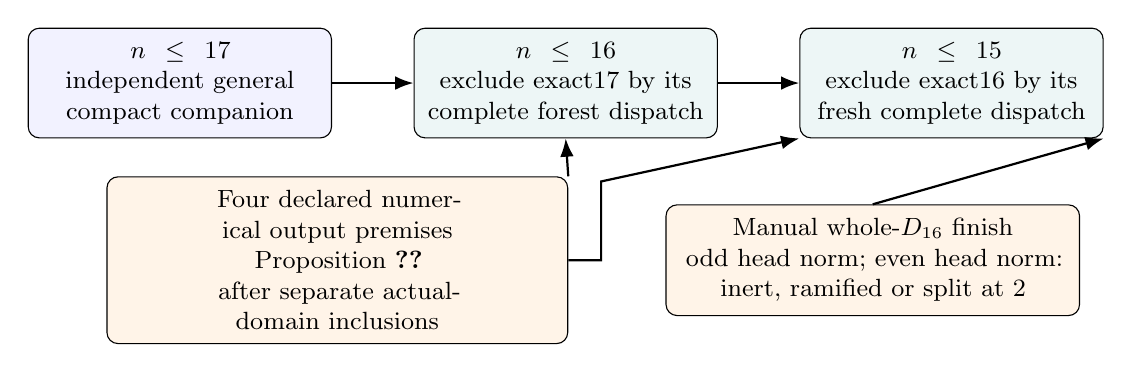
\begin{tikzpicture}[font=\small,>=Latex,
 box/.style={draw,rounded corners,align=center,minimum height=1.0cm,
 inner sep=5pt}]
 \node[box,text width=3.5cm,fill=blue!5] (general) at (1.9,3.45)
   {\(n\le17\)\\independent general\\compact companion};
 \node[box,text width=3.5cm,fill=teal!7] (sixteen) at (6.8,3.45)
   {\(n\le16\)\\exclude exact17 by its\\complete forest dispatch};
 \node[box,text width=3.5cm,fill=teal!7] (fifteen) at (11.7,3.45)
   {\(n\le15\)\\exclude exact16 by its\\fresh complete dispatch};
 \node[box,text width=5.5cm,fill=orange!9] (outputs) at (3.9,1.2)
   {Four declared numerical output premises\\
    Proposition~\ref{arith:prop:pair-output}\\
    after separate actual-domain inclusions};
 \node[box,text width=4.9cm,fill=orange!9] (dyadic) at (10.7,1.2)
   {Manual whole-\(D_{16}\) finish\\
    odd head norm; even head norm:\\
    inert, ramified or split at \(2\)};
 \draw[->,thick] (general)--(sixteen);
 \draw[->,thick] (sixteen)--(fifteen);
 \draw[->,thick] (outputs.north east)--(sixteen.south);
 \draw[->,thick] (outputs.east)--(7.25,1.2)
   --(7.25,2.2)--(fifteen.south west);
 \draw[->,thick] (dyadic.north)--(fifteen.south east);
\end{tikzpicture}
\caption{The proof of Theorem~\ref{arith:thm:main}: the compact bound
and the separate exclusions in dimensions $17$ and $16$.}
\label{arith:fig:ill20261026:a15:dispatch}
\end{figure}
% END ILLUSTRATION_20261026_A15_DISPATCH

\FloatBarrier
\section{Supplementary verification}
The finite algorithms, their domains, completeness arguments and outputs
are stated in the relevant parts of the paper. Accompanying code, finite
certificates and verification records are available in the repository
\cite{Repository}.

Selected Lean~4 modules verify internal logical and algebraic deductions.
The geometric statements, published results and specified finite-data
outputs are supplied as explicit premises.

\FloatBarrier
\appendix

\clearpage
\part{Proof appendices: finite-volume polytopes}
\setcounter{section}{0}
\renewcommand{\thesection}{A.\arabic{section}}
\renewcommand{\theHsection}{appendix-fv.\arabic{section}}

\section{Geometric coverage and exact local certificates}
\label{fv:app:routing}

The finite objects in this appendix are marked Gram diagrams and
certificates for their extensions. They are not a finite list of all
supporting forests. The extension arguments are what allow arbitrarily
many additional supporting roots. We first describe the domains and
checking predicates, then state the recorded finite propositions.
The same organization applies to the preceding rule and to the final
rule, with the final guarded consumer treated in the body of the paper.

\subsection{The complete core domain}

Generate the connected affine diagrams of ranks four through eight:
the four classical families in each rank, together with
 $\widetilde F_4,\widetilde E_6,\widetilde E_7,\widetilde E_8$.
These are 24 sources. To each source on $\ell$ roots attach a root
by every nonzero contact vector in $\{0,1,\sqrt2\}^{\ell}$.
Keep an extension exactly when it is indefinite and every one-root
deletion is a finite or affine forest. Identify labelled isomorphic
results, and retain every ordered pair of marks whose two deletions
are positive definite. This is a finite exact algorithm; isomorphism
testing may be done by trying all permutations of at most ten roots.

It is complete. A minimal indefinite core of order at least six
cannot be a compact Lann\'er diagram. It has a proper affine block;
the positive kernel and connectivity show that adjoining one adjacent
root already makes an indefinite block. Minimality therefore makes
this the whole core. A label at least five would occur in a connected
proper five-root subdiagram, forbidden by finite/affine classification.
A parallel pair with a third contacting root is already indefinite,
and a dotted pair is indefinite alone. The contact alphabet is
therefore a consequence of classification, rather than a cutoff.
Checking all one-root deletions checks every proper principal block.

For orders four and five generate every connected graph with labels
respectively 2 through 6 and 2 through 5, and apply the same acceptance
and marking tests. These alphabets follow from the finite/affine
three- and four-root lists. Order-two dotted cores are analytic
cases. For an order-three core retain the full Gram family
 \[
 \begin{pmatrix}2&-x&-u\\-x&2&-v\\-u&-v&2\end{pmatrix},
 \qquad x=2\cos(\pi/m),
\]
including the parallel endpoint $x=2$. The black--black label is
unbounded; it is not enumerated up to a numerical maximum.

\subsection{All unions and all additional cross bonds}

In a marked core $C$ put
 $\delta_C(v)=\min(d(v,a),d(v,c))$. The high-core catalogue has
 $\delta_C\le7$. In the branch with no adjacent marked path of
length at most eight, a shared white pair $(v,w)$ must satisfy
 $\delta_C(v)+\delta_D(w)\ge9$. Generate every injective partial
matching of white nodes satisfying this condition and preserving
all labelled edges and nonedges. No black node is identified.
This bounded matching loop includes failed identifications.

In the resulting union test all remaining permitted cross bonds
and all permitted multi-position subsets. A cross bond at too small
a combined distance gives an earlier short path. The inverse tests
on the positive white blocks and actual black deletions give a
finite native alphabet at every other position. For example a bond
of magnitude $b$ between two positive white blocks requires
 \[
 b^2(G_{C,W}^{-1})_{vv}(G_{D,W}^{-1})_{ww}<1.
\]
Inverse positivity makes the corresponding necessary one-contact
bounds valid even in the presence of further nonnegative contacts.

A pruning certificate must exhibit one of the following: a
nonzero nonnegative vector of nonpositive square in a block required
positive definite; a vector of strictly negative square in a corner
required positive semidefinite; negative index at least two; or a
retained adjacent marked short path. A nonnegative-vector witness
at minimum native magnitudes remains valid when further contacts
are added, since its square can only decrease. Negative index by
itself is not used as a monotonicity assertion for further bonds;
those branches are enumerated separately.

The unbounded order-three clause has an exact symbolic certificate.
Its only surviving high port has inverse diagonal zero. Eliminating
the high core gives zero Schur correction to the displayed small
Gram for every physical $x,u,v$. Its negative direction then supplies
a second negative direction. This disposes of every finite label
and the parallel endpoint at once.

\subsection{What an extension certificate means}

The common geometric lemmas in Section~\ref{fv:sec:finite-interface}
give the following complete meanings to the certificate types.
A radical certificate lists the possible contact positions and a
nonzero full-core kernel vector. Since its represented vector is
zero, every new contact annihilates it. If all allowed coefficients
are nonzero, a nonempty nonnegative contact must meet both sign
sets. The certificate lists the resulting short paths. Otherwise
every extra root is orthogonal to the core, including the first
root of any indirect extension.

An inverse certificate gives the physical core inverse $J$.
A new norm-two root with contact column $q$ has residual square
 $2-q^tJq\ge0$ in a positive-definite complement. At equality its
residual vector is zero, so all further products are fixed.
For two prospective contacts at $i,j$, compare $J_{ij}^2$ with
 $(2-J_{ii})(2-J_{jj})$; Cauchy either excludes them or forces the
displayed bond and short path. Multiple-contact exclusions use
nonnegative inverse entries in the appropriate end block.

An attached-forest certificate gives a single remaining old contact
position $p$ with $J_{pp}=r>1$. The argument of
Lemma~\ref{fv:lem:inverse} bounds the entire new rank by
 $1/(r-1)$, including indirect tails. A protected-role certificate
instead forbids a first new contact at specified incident neighbors,
thereby preserving a feature or a leaf of the \emph{whole} component.
An affine certificate supplies a positive kernel at an actual cusp;
all further supporting contacts are orthogonal to that entire factor.

Each certificate is checked in the physical Gram normalization.
Positive diagonal congruences may be used only with their norm
scales recorded. An unbounded parameter is handled by a proved
symbolic identity or a polynomial nonnegativity certificate on its
whole stated range, never by sampling.

\begin{lemma}[A terminal affine-$B$ tail]
\label{fv:lem:terminal-b-tail}
Let $K$ be a nondegenerate Lorentzian subspace of the physical root space.
Suppose that a root $e$ of squared norm $2$ has orthogonal residual
 $e_\perp$ with $e_\perp^2=\rho<1$. There cannot be a chain
 $f_1,\ldots,f_k$ of roots in $K^\perp$, each of squared norm $2$,
with $k\ge1$ and the following native products. For $k\ge2$, consecutive products
are $-1$, except for $(f_{k-1},f_k)=-\sqrt2$; also
 $(e,f_1)=-1$. For $k=1$, instead $(e,f_1)=-\sqrt2$.
All other products between distinct roots in the chain, and between
 $e$ and $f_j$ for $j>1$, are zero.
\end{lemma}

\begin{proof}
The complement $K^\perp$ is positive definite. Put
 \[
 v=f_1+\cdots+f_{k-1}+\frac{f_k}{\sqrt2}.
\]
For $k\ge2$, its diagonal terms sum to $2(k-1)+1$ and its
consecutive cross terms sum to $-2(k-1)$. Thus $v^2=1$.
For $k=1$ the same identity follows from $f_1^2=2$.
The prescribed products give $(e,v)=-1$ in both cases.
Since $v\in K^\perp$, positive-space Cauchy gives the contradiction
 \[
 1=(e_\perp,v)^2\le e_\perp^2v^2=\rho<1.
\]
Only the coefficient of the final root has changed: every physical
root still has squared norm $2$.
\end{proof}

This lemma treats a terminal chain of any length, including cases where
the first two new roots alone do not violate Cauchy. Its orthogonality
hypothesis must be proved before it is used. After excluding an adjacent
white-interior path of length at most eight, the complete contact
certificate permits a unique first root, or permits
that root together with one exterior root. In the latter case the
full no-bridge estimate bounds the whole component in the presence of
the exterior root; that bound is strictly smaller than the actual target
order. This excludes the exterior root and every indirect bridge.
First-contact uniqueness then proves successively that all later roots
are genuinely new and orthogonal to the old core. Their native zero
products can be used only after this step. If the sole old-core contact of the first root
is at $i$ with magnitude $1$ and $J_{ii}>1$, the inverse certificate gives
 $\rho=2-J_{ii}<1$.

The exact application checks the complete supplied terminal-suffix map,
all its edges and nonedges, and the original physical contact-profile
selector. A contact theorem computed for another target is used only
when its original core, ordered corner and full contact hypotheses
coincide; its old target map is never relabelled as the present one.
The terminal congruence in the calculation of $v^2$ is a rational check,
with the scale $1/\sqrt2$ recorded explicitly.

For every bounded whole component, enumerate each classical target
at every allowed rank or order, every exceptional target at its rank,
and every induced labelled embedding of its displayed subdiagram.
Assign target vertices successively and check each edge and nonedge
against the earlier assignments. Finite target size proves termination;
deleting the last assigned vertex proves completeness by induction.
The marked images select individual entries of
Appendix~\ref{fv:app:weights}, including zeros and fractions. The
displayed whole-component bound, rather than an arbitrary search cap,
proves that every actual completion is represented.

\begin{proposition}[Recorded core and extension calculations]
\label{fv:prop:local-calculations}
The preceding bounded algorithms have the following exact outputs.
The high-core generator tests 146\,262 attachments and gives 26
isomorphism classes, with order counts $12,3,4,4,3$ in orders
6 through 10 and 768 ordered finite-deletion markings. The low
order-four and order-five counts are 32 and 14.
The complete high-overlap domain has 82\,197 consistent matchings;
75\,947 inverse and 3636 edge prunings leave 2614 contexts on
154 physical cores. They have respectively 1329 radical, 823
positive-residual, 259 bounded-component, 120 isolated-inverse,
74 protected and 9 adaptive certificates. All free cross bonds
are discharged by 154\,502 short-path and 5528 edge witnesses.

Every disjoint high/high union is excluded, including all
10\,990 multi-position subsets. The low/high domain is excluded
or gives a whole component of order at most twelve or an
independent short path. Bounded affine target searches use all
1153 eligible patterns in orders 14--17, with whole-bound
multiplicities $313,354,346,140$.
The exact extension certificates satisfy the predicates just
specified. In each retained terminal configuration their chosen
\emph{current} corner contributions sum to at least one.
\end{proposition}

This is a computed proposition, supported by the separate exact
local certificates in the reproducibility package. Its assertion
includes the receipt identities and inequalities, not merely the
listed counts. The finite orders, alphabets, matchings and target
bounds prove termination. The core, union and extension arguments
prove coverage. Successful rows alone would prove neither.

\subsection{Triangles and their four exceptional markings}

% Supporting insertion, not a separate manuscript.
% Place immediately after the heading ``Triangles and their four exceptional
% markings'' in app:routing, before the historical minimal-core census.
\begin{lemma}[The reduced small affine pairs are absent from triangles]
\label{fv:lem:current-affine-triangle-exclusions}
No actual triangular two-face has an ideal corner whose varying affine
factor and marked pair are one of the following:
\begin{enumerate}
\item a cycle of order ten, marked at antipodal nodes;
\item a cycle of order eleven, marked at distance five;
\item $\widetilde D_9$ of order ten, marked at leaves of opposite forks.
\end{enumerate}
This assertion allows arbitrary additional supporting roots and other
factors of the cusp.
\end{lemma}
\begin{proof}
Let $a,b$ be the two marked roots at the ideal corner, let $F$ be its
varying affine factor, and let $c$ be the third side root of the
triangle. Normalize every root to square two. All nodes of
 $F\setminus\{a,b\}$ support the triangle. The other two actual
corner diagrams are positive semidefinite, so both principal sets
 $(F\setminus\{a\})+c$ and $(F\setminus\{b\})+c$ are positive
semidefinite.

For either positive-definite deleted-factor matrix $B$, put
 $p_j=-(c,r_j)\ge0$. Schur complementation gives
 \[
 p^TB^{-1}p\le2.
\]
The inverse is entrywise nonnegative, and every nonzero native contact
has magnitude at least one. Consequently a position with
 $(B^{-1})_{jj}>2$ cannot be contacted. This is a necessary condition
on a principal submatrix; extra supporting roots cannot repair its
failure.

Number a cycle of order $m$ by $0,\ldots,m-1$, and take $a=0,b=5$.
Deleting a node gives $A_{m-1}$, whose inverse diagonal at path
position $k$ is $k(m-k)/m$. For $m=10,11$, all positions at least
three steps from both path ends have diagonal at least
 $21/10,24/11$, respectively, both greater than two. The two
deleted-factor tests therefore give these possible contact sets:
\[
\begin{array}{c|c|c}
 m&\text{after deleting }0&\text{after deleting }5\\\hline
 10&\{1,2,8,9\}&\{3,4,6,7\}\\
 11&\{1,2,9,10\}&\{3,4,6,7\}.
\end{array}
\]
In each row the sets are disjoint. Contact to either removed mark
is forbidden by the other deletion: the relevant diagonal is
 $5/2$ at order ten and $30/11$ at order eleven. Thus $c$ is
orthogonal to every root of $F$.

For the last case number $F$ as the spine $0,\ldots,5$, with
leaves $6,7$ at $0$ and $8,9$ at $5$, and take $a=6,b=8$.
Each deletion is finite $D_9$. After deleting $6$, its only
inverse diagonals at most two occur at the long endpoint $7$
and its neighbor $0$, with values one and two. After deleting
 $8$, they occur at $9,5$ with the same values. The short-leaf
diagonals are $9/4$, and all other diagonals exceed two.
Hence the possible contact sets are $\{0,7\}$ and $\{5,9\}$,
which are disjoint. The other deletion also forbids contact to
each removed mark, again by its short-leaf diagonal $9/4$.
Thus $c$ is orthogonal to all of $F$ in this case as well.

Let $\nu=\sum_{j\in F}\delta_jr_j$, with every $\delta_j>0$,
be the positive affine-kernel combination. It is a nonzero future
null vector representing the actual ideal corner: nonzeroness
follows by pairing with a strict interior point. The third side
of a nondegenerate actual triangle does not contain that corner,
so $-(c,\nu)>0$. The orthogonality just proved instead gives
 $(c,\nu)=0$, a contradiction. Rotation and reflection cover all
cycle pairs, and fork interchange and spine reversal cover all
four opposite-fork pairs. The argument has used no restriction
on spectator rank or on the other cusp factors.
\end{proof}

We now compare the inherited triangle witnesses with the actual weights
of Appendix~\ref{fv:app:weights}. The two cycle orbits above are the only
current reductions of ideal paths of length at most five. The reduced
order-ten $D$ orbit has distance seven and is also absent from
triangles by the lemma. Every other printed replacement in affine
 $B,C,D$ of orders ten through seventeen has distance at least eight.
For larger orders the selected length-six or length-seven feature
paths retain their units: their branch or nonsimple-bond witness
persists within five steps of a mark. Such a witness cannot lie in
an affine $A$ cycle. Every affine factor of order at most nine still
pays a unit on every pair.

The four alternate witnesses below have an additional protection.
Their fixed simple leaf with a degree-two neighbor excludes every
classical affine factor, while exceptional affine factors have order
at most nine and retain full units. If the marked component is
finite, the protected leaf is at distances $2,1,0,0$ from a mark
in the four displayed cases. It remains a whole-component endpoint,
so the deep finite deletions, which require both marks to be at
least six steps from every finite feature, do not remove the unit.
The other selected finite length-six or length-seven witnesses
already have a persistent branch or nonsimple feature within five
steps. The sparse finite replacements in ranks twelve through
seventeen are all longer than these selected paths. Thus the
two-unit triangle argument below applies to the current rule,
rather than assuming that every historical short ideal pair
still has weight one.


A minimal indefinite core of an actual triangle contains all three
black roots, since every deletion of one black lies in a positive
semidefinite corner. Up to order six, a Steiner tree through the
marks gives two distinct corner paths avoiding the third black,
each of length at most five. In higher orders generate every
marked triple in every core: there are
 $3\binom73+4\binom83+4\binom93+3\binom{10}3=1025$.
Delete the third black when evaluating each corner path and feature.
The exact elementary test gives two persistent payments except
at four triples in the simple ten-node tree
 \[
 0\! -\!1,\ 0\! -\!2\! -\!3,\quad
 0\! -\!4\! -\!5\! -\!6\! -\!7\! -\!8\! -\!9.
\]
Their protected alternate pairs are
\begin{center}
\begin{tabular}{c|c|c|c}
Triple&Alternate pair&Length&Fixed leaf and neighbor\\\hline
$(0,1,9)$&$(0,9)$&6&$3,2$\\
$(0,2,9)$&$(0,9)$&6&$1,0$\\
$(1,2,8)$&$(1,8)$&6&$1,0$\\
$(1,2,9)$&$(1,9)$&7&$1,0$
\end{tabular}
\end{center}
In the first, second and fourth cases, the other corner contains
affine $E_8$ on $0,\ldots,8$ with positive kernel
 $(6,3,4,2,5,4,3,2,1)$. Kernel orthogonality forbids all additional
supporting contacts there. In the third case the finite $E_8$
inverse on $0,\ldots,7$ has diagonal
 $(30,8,14,4,20,12,6,2)$ and is entrywise nonnegative. A new native
contact at any of $0,\ldots,6$ has projection above two; only
position 7 can be contacted. The displayed leaf and its neighbor
therefore remain protected in every case.

No classical affine diagram has a simple leaf with a degree-two
neighbor. Thus the alternate lies in a finite component or in an
exceptional affine factor of order at most nine, and its unit
persists. The complete elementary test also verifies the persistent
feature for all 54 distance-six cases and the distance-seven cases.
The deep finite deletions and the sparse long-pair changes affect
none of these selected units. This proves triangle payment two.

\subsection{The order of the quadrilateral arguments}

The local statements are composed by complete face inequalities,
not by recursively replacing an obsolete corner unit.
Write $S_k$ for the assertion that a suitable adjacent marked
path of length at most $k$ makes the \emph{whole face} receive at
least one, and $F_k$ for the replacement of a deleted deep finite
length-$k$ payment. The assertion $S_k$ does not give unit weight
to that particular pair. Direct literal roles and the independent
cycle-ten and cycle-eleven arguments first prove $S_5$. Their
second halves occur at distinct corners, and their whole finite
leaves and small-factor roles have the current printed weights.
The independent near-terminal affine-$C$ zero proofs likewise
pay the entire face; their zero corner is never called a unit.

One more independent priority is essential. An opposite-fork pair
in the affine $D$ diagram of order ten contributes $27/32$, rather
than its historical unit. Its complete four-profile determinant
argument has at least one extreme end. With exactly one extreme,
full-metric Cauchy either gives a retained short path or makes its
entire spectator column empty or a single unit endpoint contact
on a whole $A_r$, $r\le3$. With two extremes, the difference
energy is $7/4$.
A close mixed component gives a distinct short-five half. The
complete far inverse spectrum leaves whole $A_{15}$ or $D_7$;
their literal corners give a restored $A_{17}$ endpoint, a protected
 $D_{25}$ unit, or a whole exceptional affine unit. In the unmixed
case choose a side of energy at most $7/8$, giving either an empty
column or one unit endpoint contact on a whole $A_r$, $r\le7$.
In either unmixed branch put $r=0$ for the empty column. If the
extreme root's old unit attachment meets the selected leaf, the
paying corner has a whole $A_{r+1}$ endpoint and a whole $D_9$
short leaf. The printed coupon is $5/32$. If instead it meets
the old mate, the corner is whole $D_{10+r}$ with a marked short
leaf at distance eight, a retained unit for every $0\le r\le7$.
These are two distinct attachment cases, not two descriptions of
the same coupon. The immediate affine alternatives also
supply a distinct literal half or $27/32$. Thus every branch pays
at least $27/32+5/32=1$, without recursively treating this corner
as a unit.

The computed inputs are the complete far inverse blocks and their
strict-gradient inequalities, all sixteen whole finite coupons, and
all twelve mixed whole-corner Gram records. Their finite domain is:
for an $A$ component, unit difference energy $d(N-d)/N\le7/4$
and strict separate inverse diagonals imply
 \[
 4\le d\le14,\qquad d+2\le N\le
       \left\lfloor\frac{4d^2}{4d-7}\right\rfloor.
\]
Enumerate every position in those ranges satisfying the strict
diagonal tests. Complete finite inverse formulas leave only
 $D_6,D_7$ and the eligible $E_6$ block outside $A$; other types
have no far allowable pair. Nonunit quadrants have their minimum
at $(\sqrt2,1)$ or $(1,\sqrt2)$, by the recorded positive gradients
and positive quadratic remainder. Their minima exceed $7/4$.
All loops are finite and the inverse bounds prove coverage; the
literal Gram records check every actual corner and its whole
marked role. These inputs are not inferred from the counts in
Proposition~\ref{fv:prop:local-calculations}.

The remaining dependency order is
 \[
 S_5\ \longrightarrow\ F_6\ \longrightarrow\ S_6
 \ \longrightarrow\ F_7\ \longrightarrow\ S_7
 \ \longrightarrow\ F_8\ \longrightarrow\ S_8.
\]
Here $S_6$ uses the cycle cases with shorter arc six, including the
order-fourteen case, together with $F_6$. The protected affine-$D$
order-ten terminal of $F_7$ invokes the independent priority just
proved. Before using $S_7$, prove the cycle arcs $(7,8)$ rectangle
bound separately: a required neighboring contact gives a Cauchy
correction on one fixed side of the entire rectangle. The corrected
quadratic remains concave in reciprocal heights. This calculation
has no $F_8$ premise, even though its certificate shares a file with
that later composition. For arcs $(7,7)$ the sealed equality corners
currently pay $41/64+23/64=1$, rather than two historical halves.
The affine-tree cases use their persistent branch or nonsimple-bond
features and the independent small-factor priorities. Finally the
strict $F_8$ corridor ends at $S_7$, after which the remaining cycle
and tree cases prove $S_8$. All additional supporting contacts are
controlled by the whole-component seals, not by an ambient-rank cap.
The large finite-$D$ leaf-nine half has its own distinct small/$D_{10}$
half; it is not used as a unit.

For a small affine factor, its positive kernel first splits off
the spectator forest. Adjacent black contact or a shared spectator
neighbor gives an earlier short path. Otherwise the two spectator
columns have disjoint support. The complete inverse-diagonal
profiles and four-root Schur determinant give a strict obstruction
or a closed equality system. At equality Gram Cauchy determines
the active whole spectator types. These are the bounded profile
calculations in Proposition~\ref{fv:prop:local-calculations}, with
unbounded native magnitudes retained symbolically. A changed
affine-$B$ corner invokes its independent full-face theorem before
a later affine-$D$ theorem can spend that corner's old half.
An immediate affine alternative within one equality receipt
contributes its current fraction at a distinct corner and makes
no recursive theorem call.

Finally the finite sparse substitutions are single inequalities
on all four actual corners. Their relevant contribution lists
are $(1/2,1/4,1/4,0)$, $(0,1/8,1/4,5/8)$ and
 $(0,1/4,1/4,1/2)$, each summing to one. The extension seals
prove the whole context witnesses at the positive corners.
If a witness is absent, that branch is excluded or independently
paid; an induced small subgraph cannot serve as a witness.
The full chosen-role checks cover the 216 literal stars, 564
later corners, 24 $D_{14}$ variants and 332 positive $D_{12}$
outputs. Universal outputs outside those fixed Gram lists use
their whole-factor profile proofs. In particular, the affine-$B$
singleton consumers of $B_{13}(0,12)$ have a distinct sealed
 $A_1/D_{12}$ unit, and the quiet affine-$D_{12}$ consumer of the
guarded $D_{13}$ half is proved in the body of the paper.

This order is well founded: independent face payment, shorter-path
or protected terminal payment, whole-factor profile system, then
joint finite receipt. A joint receipt is one terminal inequality,
not a call back to another decreased role. Every actual quadrilateral
either ends at an earlier face theorem or reaches a union and
extension certificate in the complete generated domain. Its
distinct current contributions total at least one. This proves
the local coverage used in Proposition~\ref{fv:prop:oldcount} and,
with Theorem~\ref{fv:thm:local}, the final rule. It uses the recorded
distributed certificates; no new flattened certificate run is
assumed or claimed.

\section{The intrinsic corner weights}\label{fv:app:weights}

We specify a single function of the actual marked vertex diagram.
At a finite vertex let $\mathcal F$ be the full spherical forest,
with two marked nodes $a,b$. In one whole component use the
same-component entry below. In distinct components use the ordinary
cross entry and the stated contextual additions. At a cusp use only
the affine table for its varying factor, with the multiplicity proved
in Section~\ref{fv:sec:finite-interface}. An omitted role has weight zero.

Number $A_r$ by $0,\ldots,r-1$, and $B_r$ by the same path with
its last bond doubled. Number $D_r$ by the spine $0,\ldots,r-3$
with leaves $L_r=\{r-2,r-1\}$ at the center $r-3$; its long end is 0.
For an $A_r$ factor put $E_r=\{0,r-1\}$ and
 $P_k(A_r)=\{k-1,r-k\}$, removing repetitions. The long ends of
 $E_6$ lie on its two length-two arms. The tables are invariant
under diagram automorphisms.

\subsection{Finite same-component entries}
Every pair in a component of rank at most 11 has weight one;
this includes $I_2(m)$ for every $m\ge5$.
For classical rank $r\ge18$, a feature is a vertex of degree
other than two, or an endpoint of a nonsimple bond. Put
 $\delta(v)=\operatorname{dist}(v,\text{features})$.
Start with one at distance at most eight and at distance nine
containing a whole-component leaf. Delete the unit at distance
6, 7 or 8 when both marks have $\delta\ge6$.
In $D_r$, $r\ge20$, halve each distance-nine pair containing a
short fork leaf. These are all ordinary large-rank entries.
Their sums, with $x_+=\max(x,0)$, are
 \begin{align*}
 B(A_r)&=8r-34-(r-18)_+-(r-19)_+-(r-20)_+,\\
 B(B_r)&=8r-34-(r-19)_+-(r-20)_+-(r-21)_+,\\
 B(D_r)&=8r-32-[r\ge20]-(r-20)_+-(r-21)_+-(r-22)_+.
\end{align*}
For ranks 12--17 start with all units and make exactly the following
replacements. Z, H, Q, O mean $0,1/2,1/4,1/8$; A13 means
 $A_{13}$, and similarly for the other labels. Unlisted entries
retain one. The $B_{17}$ convention is stated separately.

{\small
\begin{verbatim}
D12 H: (0,10),(0,11).

A13 Z: (0,12).
B13 Z: (0,12).
D13: no ordinary replacement.

A14 Z: (0,12),(1,13),(0,13).
B14 Z: (0,13),(1,13),(2,13),(3,13).
D14 Z: (0,12),(0,13); H: (0,11).

A15 Z: (0,12),(0,14),(2,14),(0,13),(1,14).
B15 Z: (0,12),(0,13),(0,14),(1,13),(1,14),(2,14),(3,14),(4,14).
D15 Z: (0,11),(1,13),(1,14);
    H: (0,12),(0,13),(0,14),(1,12).

A16 Z: (0,12),(0,14),(0,15),(1,14),(1,15),(3,15),(1,12),(3,14);
    H: (0,13),(1,13),(2,14),(2,15);
    O: (0,11),(4,15).
B16 Z: (0,11),(0,12),(0,13),(0,14),(0,15),
       (1,12),(1,13),(1,14),(1,15),(2,13),(2,14),(2,15),
       (3,14),(3,15),(4,15),(5,15).
D16 Z: (0,10),(0,11),(0,12),(0,13),(1,11),(2,12),(2,14),(2,15);
    H: (0,14),(0,15),(1,12),(1,13),(1,14),(1,15),(2,13).

A17 Z: (0,10),(0,11),(0,12),(0,14),(0,15),
       (1,10),(1,11),(1,13),(1,14),(1,16),
       (2,12),(2,14),(2,15),(2,16),(3,15),(4,14),(4,16),
       (5,15),(5,16),(6,15),(6,16);
    H: (0,16),(2,13),(3,14);
    weight7/8: (1,12),(4,15).
D17 Z: (0,10),(0,11),(0,12),(0,13),
       (1,10),(1,11),(1,12),(1,13),(1,14),(1,15),(1,16),
       (2,12),(2,14),(3,15),(3,16),(4,14),(4,15),(4,16);
    H: (0,14),(2,13),(2,15),(2,16),(3,13),(3,14);
    Q: (0,15),(0,16).
\end{verbatim}
}
For $B_{17}$ keep one exactly at distance at most eight, at
distance nine containing a whole-component leaf, and at
 $(2,11),(3,12),(4,13)$. All other entries are zero.
The ordinary same-component sums are
\begin{center}
\begin{tabular}{c|rrrrrr}
$r$&12&13&14&15&16&17\\\hline
$A_r$&66&77&88&100&$433/4$&$453/4$\\
$B_r$&66&77&87&97&104&105\\
$D_r$&65&78&$177/2$&100&$217/2$&$227/2$
\end{tabular}
\end{center}
For Proposition~\ref{fv:prop:oldcount} alone restore $B_{13}(0,12)=1$,
so that its preliminary sum is 78. The final rule uses the zero
entry above. This is the only ordinary-table difference in that
preliminary calculation.

\subsection{Ordinary cross-component roles}
The table is symmetric in the two marked components. A product
of mark sets means every pair in that product. In the first seven
rows $S$ is any irreducible component of rank at most five, and
 $\mathrm{all}(S)$ is its node set. Apply those broad rows first,
then replace values where a later row applies. Later rows are
replacements, not additions; overlaps never disagree. All unlisted
roles are zero. An arbitrary $I_2(m)$ is a small rank-two type,
but is not an $A_2$ where that type is expressly named.

{\small
\begin{longtable}{p{.36\textwidth}p{.43\textwidth}r}
\toprule First component and marks&Second component and marks&Weight\\\midrule
\endhead
 S,$\mathrm{all}(S)$ & $D_{10}$,$L_{10}$ & $1/2$ \\
 S,$\mathrm{all}(S)$ & $D_{11}$,$D_{12}$,$D_{13}$,$D_{14}$, center and short leaves & $1/2$ \\
 S,$\mathrm{all}(S)$,$\operatorname{rank}(S)\le2$ & $D_{15}$,center and short leaves & $1/2$ \\
 S,$\mathrm{all}(S)$,$3\le\operatorname{rank}(S)\le5$ & $D_{15}$,$L_{15}$ & $1/2$ \\
 $A_{1}$ & $D_{16}$,center and short leaves & $1/2$ \\
 S,$\mathrm{all}(S)$ & $A_{13}$ central node 6 or $A_{15}$ central node 7 & $1/2$ \\
 S,$\mathrm{all}(S)$ & $A_{17}$,marks5,11 & $1/2$ \\
 $A_{1}$ or $A_{2}$,all marks & $D_{11}$,$L_{11}$ & $1$ \\
 $A_{4}$,$E_{4}$ & $D_{11}$,$L_{11}$ & $1$ \\
 $A_{5}$,$P_{2}$ & $D_{11}$,$L_{11}$ & $1$ \\
 $E_{6}$,long ends & $D_{11}$,$L_{11}$ & $1$ \\
 $D_{5}$,long endpoint0 & $D_{11}$,$L_{11}$ & $1$ \\
 $A_{1}$ & $D_{12}$,$L_{12}$ & $1$ \\
 $D_{5}$,$L_{5}$ & $D_{12}$,center and short leaves & $1$ \\
 $A_{2}$,all marks & $D_{13}$,$L_{13}$ & $1$ \\
 $A_{2}$,all marks & $D_{13}$,center10 & $23/64$ \\
 $A_{1}$ or $A_{4}$,$E_{4}$ & $D_{13}$,mark9 & $1/2$ \\
 $A_{1}$ or $A_{2}$,all marks & $D_{14}$,mark10 & $1/2$ \\
 $A_{1}$ & $D_{14}$,mark9 & $1/16$ \\
 $A_{1}$ & $D_{15}$,mark11 & $1/16$ \\
 $A_{2}$,all marks, or $A_{3}$,central node 1 & $D_{10}$,center7 & $1$ \\
 $A_{1}$ or $A_{2}$,all marks, or $A_{3}$,$E_{3}$ or $A_{4}$,$E_{4}$ & $B_{9}$,doubled terminal8 & $1/2$ \\
 $A_{1}$ & $B_{10}$,doubled terminal9 & $1$ \\
 $A_{2}$,all marks & $B_{10}$,doubled terminal9 & $1/2$ \\
 $A_{1}$ & $B_{11}$,mark9 & $1/2$ \\
 $A_{1}$ & $B_{12}$,mark9 & $1/2$ \\
 $A_r,E_r$, $1\le r\le8$ & $D_{9}$,$L_{9}$ & $5/32$ \\
 $A_r,E_r$, $1\le r\le4$ & $A_{9}$,central node 4 & $1/2$ \\
 $A_{1}$ & $A_{11}$,central node 5 & $1$ \\
 $A_{2}$,all marks & $A_{11}$,central node 5 & $1/2$ \\
 $A_{1}$ or $A_{2}$,all marks, or $A_{4}$,$E_{4}$ & $A_{11}$,$E_{11}$ & $1/2$ \\
 $E_{6}$,long ends, or $D_{5}$,long end0 & $A_{11}$,$P_{2}$ & $1$ \\
 $A_{1}$ & $A_{12}$,marks5,6 & $1$ \\
 $A_{1}$ & $A_{12}$,$E_{12}$ & $1/4$ \\
 $A_{4}$,$E_{4}$ & $A_{12}$,$E_{12}$ or $A_{12}$,$P_{3}$ & $1$ \\
 $D_{5}$,long end0 & $A_{12}$,$P_{2}$ & $1$ \\
 $D_{5}$,long end0 & $A_{12}$,$E_{12}$ & $3/8$ \\
 $D_{5}$,$L_{5}$ & $A_{12}$,$P_{3}$ & $1$ \\
 $A_{1}$ & $A_{13}$,central node 6 & $41/64$ \\
 $A_{2}$,all marks & $A_{13}$,central node 6 & $23/64$ \\
 $A_{1}$ & $A_{13}$,$E_{13}$ & $1/2$ \\
 $A_{1}$ & $A_{13}$,$P_{2}$ & $1/4$ \\
 $A_{2}$,all marks & $A_{13}$,$E_{13}$ & $1$ \\
 $A_{4}$,$E_{4}$ & $A_{13}$,$P_{2}$ & $1$ \\
 $A_{4}$,internal marks1,2 & $A_{13}$,$P_{2}$ & $1/2$ \\
 $A_{2}$,all marks & $A_{14}$,$P_{2}$ or $A_{14}$,$P_{3}$ & $1/2$ \\
 $A_{1}$ & $A_{14}$,$P_{3}$ or $A_{14}$,$P_{4}$ & $1/2$ \\
 $A_{1}$ & $A_{15}$,$P_{3}$ & $1/2$ \\
 $A_{1}$ & $A_{16}$,$P_{4}$ & $1/2$ \\
 $A_{1}$ & $A_{16}$,$E_{16}$ & $1/4$ \\
\bottomrule
\end{longtable}
}
For example, the $D_5$ long-end/$D_{12}$ center entry is one half;
the upgrade to one concerns short $D_5$ leaves. There is no
ordinary $A_1/B_8$ payment.

\subsection{Contextual entries}
Every witness is a distinct unmarked whole component at the actual
corner. Presence is Boolean. The first table replaces ordinary
same-component values; the second adds to cross roles whose
ordinary values are zero.

{\small
\begin{longtable}{>{\raggedright\arraybackslash}p{.35\textwidth}>{\raggedright\arraybackslash}p{.43\textwidth}>{\raggedright\arraybackslash}p{.12\textwidth}}
\toprule Marked component and pair&Presence guard&Value\\\midrule
\endhead
 $A_{13}$,(0,12) & $A_{1}$ present & $1$ \\
 $A_{14}$,(0,13) & $A_{1}$ present & $1/2$ \\
 $A_{15}$,(0,13),(1,14) & $A_{1}$ present & $1/4$ \\
 $D_{15}$,(1,13),(1,14) & $A_{1}$ present & $1/4$ \\
 $A_{16}$,(1,12),(3,14) & $A_{1}$ present & $5/8$ \\
 $D_{16}$,(0,14),(0,15) & $A_{1}$ present & $1$ \\
 $D_{14}$,(0,12),(0,13) & $A_{1}$ or $A_{2}$ or $A_{3}$ present & $1/2$ \\
 $D_{13}$,(0,11),(0,12) & at least three $A_{15}$/$D_{15}$ components & $1/2$ \\
 $D_{28}$,(0,12) & at least two $A_{15}$/$D_{15}$ components & ordinary $+1/2$ \\
\bottomrule
\end{longtable}
\begin{longtable}{>{\raggedright\arraybackslash}p{.35\textwidth}>{\raggedright\arraybackslash}p{.43\textwidth}>{\raggedright\arraybackslash}p{.12\textwidth}}
\toprule Marked pair&Presence guard&Addition\\\midrule
\endhead
 $A_{4}$ endpoint/$A_{12}$ second node & $A_{1}$ present & $1/8$ \\
 $A_{2}$ mark/$A_{4}$ endpoint & $A_{1}$ and $A_{10}$ present & $1/4$ \\
 $A_{2}$ mark/$D_{5}$ long endpoint & $A_{1}$ and $A_{9}$ present & $1/2$ \\
 $A_{1}$/$D_{5}$ long endpoint & $A_{11}$ present OR both $A_{9}$,$A_{2}$ present & $3/8$ \\
 $A_{1}$/$D_{5}$ long endpoint & $A_{9}$ and $A_{2}$ present & $5/8$ \\
 two distinct $A_{2}$ components,any marks & $A_{10}$ and at least two $A_{1}$ present & $9/32$ \\
 $A_{12}$ endpoint/$D_{16}$ long endpoint & at least two $A_{15}$/$D_{15}$ present & $1/2$ \\
\bottomrule
\end{longtable}
}
The two $A_1/D_5$ additions deliberately add to one under the
joint $A_9,A_2$ guard; $A_{11}$ does not repeat the $3/8$ term.
The $A_2/A_2$ marks lie in distinct components.

These tables define $b(T)$ and $j(T,U)$ in~\eqref{fv:eq:forest-cost}:
$b(T)=64B(T)$ sums ordinary same-component entries, and $j(T,U)$
is 64 times the sum of ordinary cross entries on two distinct
components. For the preliminary calculation make only the stated
 $B_{13}$ restoration and omit the three rank-15-guarded changes.
Counting the other contextual pairs gives exactly $\Psi$ in
Appendix~\ref{fv:app:finite-contexts}; for example the $A_2/A_2$
row costs $64\cdot4(9/32)\binom{a_2}{2}=36a_2(a_2-1)$.
The final additional context cost is
 \[
 -64d_{13}[a_{15}+d_{15}\ge3]
 +(32d_{28}+64a_{12}d_{16})[a_{15}+d_{15}\ge2].
\]
This identifies one function feeding both geometry and maximization.

\subsection{Affine factors}
Let $m$ be the order, so the affine rank is $m-1$.
Number $\widetilde A$ as the cycle $0,\ldots,m-1$;
$\widetilde B$ as spine $0,\ldots,m-3$, double bond $(m-4,m-3)$,
and leaves $m-2,m-1$ at 0;
$\widetilde C$ as the path $0,\ldots,m-1$ with both end bonds
doubled; and $\widetilde D$ as spine $0,\ldots,m-5$ with leaves
 $m-4,m-3$ at 0 and $m-2,m-1$ at $m-5$.
In the following table A, B, C, D mean these affine families.

Every pair in order at most nine has weight one, including every
exceptional affine type. For $\widetilde A$ at order ten halve
its five antipodal pairs; at order eleven halve its eleven
distance-five pairs; at every order at least twelve retain exactly
distance at most five. For B, C, D at orders 10--17 start with
all units and make these replacements. XxY is a Cartesian product.

{\small
\begin{verbatim}
m10:
 B H:(7,8),(7,9).
 C Z:(0,9).
 D weight27/32: {6,7}x{8,9}.

m11:
 B Z:(8,9),(8,10).
 C Z:(0,9),(0,10),(1,10).
 D H:{7,8}x{9,10}.

m12:
 B Z:(0,9),(9,10),(9,11); H:(8,10),(8,11).
 C Z:(0,10),(0,11),(1,10),(1,11).
 D Z:{8,9}x{10,11}.

m13:
 B Z:(0,10),(9,11),(9,12),(10,11),(10,12);
   H:(1,10),(8,11),(8,12).
 C Z:(0,10),(0,11),(0,12),(1,11),(1,12),(2,10),(2,12).
 D Z:(0,8),{9,10}x{11,12};
   H:(0,11),(0,12),(8,9),(8,10).

m14:
 B Z:(0,10),(0,11),(1,10),(1,11),(2,11),
     (9,12),(9,13),(10,12),(10,13),(11,12),(11,13).
 C Z:(0,10),(0,11),(0,12),(0,13),(1,11),(1,12),(1,13),
     (2,11),(2,12),(2,13),(3,13).
 D Z:(0,9),(0,12),(0,13),(9,10),(9,11),{10,11}x{12,13};
   H:(1,12),(1,13),(8,10),(8,11).

m15:
 B Z:(0,11),(0,12),(1,11),(1,12),(2,12),(3,12),
     {9,10,11,12}x{13,14}.
 C Z:all path pairs of distance>=10 except (2,12).
 D Z:(0,10),(0,13),(0,14),(1,13),(1,14),
     (9,11),(9,12),(10,11),(10,12),{11,12}x{13,14};
   weight15/16:(2,13),(2,14),(8,11),(8,12).

m16:
 B Z:all pairs of graph distance>=10.
 C Z:all path pairs of distance>=10 except (1,11),(4,14).
 D Z:(0,11),(0,14),(0,15),(2,14),(2,15),(9,12),(9,13),
     (11,12),(11,13),{12,13}x{14,15};
   H:(0,9),(0,10),(1,11),(2,11);
   weight7/16:(1,14),(1,15),(10,12),(10,13).

m17:
 B Z:all pairs of graph distance>=10.
 C Z:all path pairs of distance>=10.
 D Z:(0,10),(0,12),(0,15),(0,16),(1,11),(2,12),
     (3,15),(3,16),(9,13),(9,14),(12,13),(12,14),
     {13,14}x{15,16};
   H:(0,11),(1,12),(1,15),(1,16),(11,13),(11,14);
   weight1/8:(2,15),(2,16),(10,13),(10,14).
\end{verbatim}
}
For classical affine order at least 18, features are branching
vertices and endpoints of nonsimple bonds. A simple endpoint alone
is not an affine feature. With $\delta$ the distance to this set,
keep a unit exactly when
 \[
 d(a,b)\le5\quad\text{or}\quad
 6\le d(a,b)\le9\ \text{ and }\min(\delta(a),\delta(b))\le5.
\]
All other entries are zero. A featureless cycle retains only
distance at most five. There are no ideal context bonuses.
Summing each table, taking the family maximum and dividing by
order gives exactly $c(r)$ in Section~\ref{fv:sec:ideal}; the
large-rank counts give its formula for $r\ge24$. Its geometric
use is the factor-fiber argument establishing~\eqref{fv:eq:envelope}.

\section{Contexts in the finite-forest calculation}
\label{fv:app:finite-contexts}

This appendix specifies the finite algorithm behind
Proposition~\ref{fv:prop:oldcount}. It concerns the rule before the
last $B_{13}$ and three-rank-15 changes. All charges are multiplied
by 64. Put $a_i=m_{A_i}$ and $d_i=m_{D_i}$, and write $[E]$ for
the indicator of a condition $E$. The complete additional context
cost in~\eqref{fv:eq:forest-cost} is
 \begin{align*}
\Psi(m)={}&36a_2(a_2-1)[a_1\ge2,\ a_{10}>0]
       +64a_2d_5[a_1>0,\ a_9>0]\\
 &+24a_1d_5[a_{11}>0\text{ or }(a_9>0,\ a_2>0)]
       +40a_1d_5[a_9>0,\ a_2>0]\\
 &+32(a_{15}+d_{15})[a_1>0]
       +64d_{14}[a_1+a_2+a_3>0]\\
 &+[a_1>0]\bigl(80a_{16}+32a_{14}+64d_{16}+64a_{13}\\
 &\hspace{4.7em}+32a_4a_{12}+64a_2a_4[a_{10}>0]\bigr).
\end{align*}
Witness presence is Boolean. Additional witnesses multiply a bonus
only where an actual multiplicity occurs in this formula.

\subsection{Representatives and actual fibers}

Use $E_6$ as the rank-six representative and $B_9$ as the rank-nine
representative. At rank 12 identify $A_{12},B_{12}$ with $A_{12}$,
but keep $D_{12}$ separate. Keep $A_{17}$ separate from the other
rank-17 types. At all remaining ranks at most eight use the type
 $A$ of that rank; at larger ranks use the type $D$ of that rank.
The fixed representatives are generated by the integer domain
 \[
 c_9,\ldots,c_{17}\ge0,\quad
 \sum_{r=9}^{17}rc_r\le58,\quad
 0\le k_{12}\le c_{12},\quad
 0\le k_5\le\left\lfloor
       \frac{58-\sum_{r=9}^{17}rc_r}{5}\right\rfloor.
\]
They consist of $c_9$ copies of $B_9$, $c_{10}$ copies of $D_{10}$,
$c_{11}$ copies of $D_{11}$, $k_{12}$ copies of $A_{12}$,
$c_{12}-k_{12}$ copies of $D_{12}$, $c_r$ copies of $D_r$ for
 $13\le r\le16$, $c_{17}$ copies of $A_{17}$, and $k_5$ copies
of $A_5$. The split $k_{12}$ counts representative $A_{12}$ components:
before actual-type expansion it combines actual $A_{12}$ and $B_{12}$,
and is distinct from the actual multiplicity $a_{12}$ in $\Psi$.
The residual ranks are
 \[
 \{1,2,3,4,6,7,8\}\ \cup\ \{17,\ldots,58\}.
\]
Thus residual rank 17 represents $B_{17},D_{17}$, whereas the
 $A_{17}$ count is already fixed. These conventions matter for
the context bonuses.

% Supporting insertion, not a separate manuscript.
\subsection{The numerical coarse screen}\label{fv:app:coarse-screen}

The coarse coefficients differ from the actual coefficients $b,j$:
they include allowances for some presence guards. We define them here,
so the preliminary screen is a finite numerical problem as well as a
description of its output. Barred quantities are unscaled payments;
multiplication by 64 gives integer coefficients.
For the fixed multiset $F$ and remaining rank $R$ just defined, put
 \[
 \mathcal R=\{1,2,3,4,6,7,8\}\cup\{17,\ldots,58\},\qquad
 u_r=\begin{cases}E_6&r=6,\\ A_r&r\le8,\ r\ne6,\\D_r&r\ge17.
 \end{cases}
\]
The fixed base coefficients are
\begin{center}
\begingroup\small\setlength{\tabcolsep}{3pt}
\begin{tabular}{c*{11}{r}}
\toprule
$T$&$A_5$&$B_9$&$D_{10}$&$D_{11}$&$A_{12}$&$D_{12}$&$D_{13}$&$D_{14}$&$D_{15}$&$D_{16}$&$A_{17}$\\
\midrule
$\bar b(T)$&$10$&$36$&$45$&$55$&$66$&$65$&$78$&$179/2$&$201/2$&$219/2$&$3613/32$\\
\bottomrule
\end{tabular}
\endgroup
\end{center}
For residual types, $\bar b(u_r)=\binom r2$ for $r\in\mathcal R$, $r\le8$,
while
 \begin{align*}
 \bar b(D_{17})&=919/8,\\
 \bar b(D_r)&=8r-32-[r\ge20]
       -(r-20)_+-(r-21)_+-(r-22)_+\qquad(r\ge18),
\end{align*}
where $x_+=\max(x,0)$. The symmetric interaction table is as follows.
Omitted entries are zero, including every interaction of two large fixed
types and every interaction involving a residual $D_r$, $r\ge17$.
\begin{center}
\begingroup\small\setlength{\tabcolsep}{3pt}
\begin{tabular}{c*{11}{r}}
\toprule
&$A_5$&$B_9$&$D_{10}$&$D_{11}$&$A_{12}$&$D_{12}$&$D_{13}$&$D_{14}$&$D_{15}$&$D_{16}$&$A_{17}$\\
\midrule
$A_1$&$3/8$&$1/2$&$1$&$5/2$&$5/2$&$5/2$&$137/64$&$33/16$&$25/16$&$3/2$&$1$\\
$A_2$&$0$&$1$&$4$&$5$&$0$&$3$&$151/32$&$4$&$3$&$0$&$2$\\
$A_3$&$0$&$1$&$4$&$9/2$&$0$&$9/2$&$9/2$&$9/2$&$3$&$0$&$3$\\
$A_4$&$0$&$1$&$4$&$8$&$17/2$&$6$&$8$&$6$&$4$&$0$&$4$\\
$A_5$&$0$&$5/8$&$5$&$19/2$&$27/4$&$21/2$&$15/2$&$15/2$&$5$&$0$&$5$\\
$E_6$&$0$&$5/8$&$0$&$4$&$0$&$0$&$0$&$0$&$0$&$0$&$0$\\
$A_7$&$0$&$5/8$&$0$&$0$&$0$&$0$&$0$&$0$&$0$&$0$&$0$\\
$A_8$&$0$&$5/8$&$0$&$0$&$0$&$0$&$0$&$0$&$0$&$0$&$0$\\
\bottomrule
\end{tabular}
\endgroup
\end{center}
Thus the $A_1/A_5$ entry is an unconditional upper allowance, not an
ordinary payment. Set
 \[
 K(F)=\sum_{T\in F}\bar b(T)
           +\sum_{\{T,U\}\subset F}\bar j(T,U),\qquad
 w_F(r)=\bar b(u_r)+\sum_{T\in F}\bar j(u_r,T).
\]
Multiset sums count distinct occurrences, including equal types. In
particular $K(F)$ includes all interactions of the fixed $A_5$ copies
with the large fixed components. Residual representatives have no mutual
interaction. Let $V_F$ be the exact-rank Bellman table with items
 $(r,w_F(r))$, $r\in\mathcal R$, and let $V_F^{\neg2}$ omit rank two.
Both are instances of Proposition~\ref{fv:prop:dp-certificate}, after scaling
by 64.

There remain two context terms. For $s\in\{1,2\}$ set
 \[
 G_0=[s=2,\ c_{10}>0],\qquad G_1=[c_9k_5>0].
\]
An admissible reservation has $s\le R$, $G_0+G_1>0$, and $s=2$ only if
 $G_0=1$. For every $0\le j\le\lfloor(R-s)/2\rfloor$ form
 \[
 L_{s,j}=s w_F(1)+j w_F(2)+V_F^{\neg2}(R-s-2j)
                 +\frac9{16}j(j-1)G_0+jk_5G_1.
\]
Here $j$ counts all rank-two representatives: every actual rank-two
type, including $B_2$ and the common dihedral symbol, maps to $u_2=A_2$.
It can exceed the actual $A_2$ count. Ignoring unreachable states, the
coarse value is
 \begin{equation}\label{fv:eq:coarse-screen-value}
 U(F)=K(F)+\frac{11}{32}c_{17}
        +\max\bigl\{V_F(R),\ L_{s,j}: (s,j)\text{ admissible}\bigr\}.
\end{equation}
The $11/32=22/64$ increment per fixed $A_{17}$ is separate from
 $\bar b(A_{17})$. These formulas define the recorded 3298-way screen
and its 39 classes with $U(F)>377$.

Here is the complete domination test behind this upper problem. Write
 $B(T)=b(T)/64$, $J(T,U)=j(T,U)/64$ for the preliminary actual rule, and
let $\rho$ be the representative map. Put
 \[
 g(A_{13})=g(D_{14})=g(D_{16})=1,\quad
 g(A_{14})=g(A_{15})=g(D_{15})=\tfrac12,\quad g(A_{16})=\tfrac54,
\]
and $g=0$ otherwise. These are the additional same-component allowances
from the presence guards, rather than their full replacement values.
Let $h$ be symmetric, with $h(A_1,D_5)=3/8$,
$h(A_4,A_{12})=1/2$, and all other entries zero. The finite comparison
checks, for every actual type and every actual type pair,
\begin{align*}
 B(T)+g(T)&\le\bar b(\rho T)+\tfrac{11}{32}[T=A_{17}],\\
 J(T,U)+h(T,U)&\le\bar j(\rho T,\rho U).
\end{align*}
This states the full domain and inequalities of the coefficient check;
it is not a comparison only of the eventual maximizing forests.

Outside the two separately bounded families below, the remaining
contexts are exactly the $A_2/A_2$ and $A_2/D_5$ terms in $L_{s,j}$.
If the first occurs, reserve two $A_1$ and choose $s=2$; this also
includes the second term whenever it occurs. If only the second occurs,
reserve one $A_1$ and choose $s=1$. Choose $j$ to be the complete rank-two
representative count. Actual $A_2$ counts are at most $j$, actual $D_5$
counts are at most $k_5$, and actual $A_9,A_{10}$ presence implies the
corresponding representative presence. Monotonicity of $j(j-1)$ and
 $jk_5$ on nonnegative integers proves domination. If neither context
occurs, $V_F(R)$ suffices. Further $A_1$ copies remain available in the
residual table; they do not multiply a Boolean witness bonus.
The reservations jointly cover every actual forest in this complement;
an individual branch need not bound another formal reconstruction.
The additional $5/8$ on $A_1/D_5$ under the joint $A_9,A_2$ guard and
the $A_1,A_2,A_4,A_{10}$ family are covered by their separate complete
conditional calculations, including overlap. No actual attainment of
the coarse upper bound is asserted.

The ordinary component and interaction inequalities give an upper
relaxation for every representative choice. The table check uses
every actual type, including the common-cost dihedral symbol;
it is not a comparison of only the eventual maximizers. It
retains the separate increment of 22 per fixed $A_{17}$. There
are 1295 fixed large vectors, 3298 choices after adjoining the
rank-five count, and two residual tables per choice, one allowing
 $A_2$ and one excluding it. Every such table is checked by
Proposition~\ref{fv:prop:dp-certificate}.

\subsection{The actual fibers of the remaining classes}

Exactly 39 coarse classes can exceed 377, outside the two context
families below. Expand \emph{every} component of each such class
into its full actual-type fiber. For repeated representatives
choose a nondecreasing list of actual types. This enumerates all
748 fixed actual multisets $F$ without losing mixed assignments.
Let $R=58-\operatorname{rank}(F)$ and enumerate the complete actual
counts
 \[
 0\le a_1\le R,\qquad
 0\le a_2\le\left\lfloor\frac{R-a_1}{2}\right\rfloor.
\]
Remove both $A_1$ and $A_2$ from the residual alphabet. If
 $a_1,a_2>0$ and $F$ contains $A_{10}$, also exclude residual
 $A_4$: those forests belong to the second family below.

At these fixed counts the only remaining presence condition is
the $D_{14}$ bonus triggered by $A_3$, when $a_1=a_2=0$ and $F$
contains $D_{14}$. Split this case into no $A_3$, or at least one
 $A_3$. In the second branch reserve one $A_3$ and charge the bonus
 $64m_{D_{14}}$ once; further $A_3$ copies remain ordinary residual
items. In the first branch exclude $A_3$ entirely.

For an allowed residual type $T$, set
 \[
 w_F(T)=b(T)+\sum_{U\in F}j(T,U).
\]
Every ordinary interaction between residual types is zero, as
checked on the whole residual alphabet. If $a_1>0$, a residual
 $A_4$ additionally receives $32m_{A_{12}}$. All other terms of
 $\Psi$ have become fixed. With $\epsilon\in\{0,1\}$ denoting the
reserved-$A_3$ branch, evaluate
 \begin{align*}
 C^{\rm ord}_{64}(F)&+a_1w_F(A_1)+a_2w_F(A_2)
       +\Psi(F+A_1^{a_1}+A_2^{a_2})\\
 &+\epsilon\bigl(w_F(A_3)+64m_{D_{14}}\bigr)
       +V(R-a_1-2a_2-3\epsilon).
\end{align*}
Here $C^{\rm ord}_{64}$ omits $\Psi$, and $V$ uses the adjusted
residual weights. Ignore unreachable final ranks. The two $A_3$
branches are used only in the specified case, so the displayed
 $\Psi$ has not already charged their bonus.

Every forest in this domain determines a branch: remove its
fixed components, all its $A_1,A_2$ components, and one $A_3$
exactly when required. Conversely a reachable residual multiset
reconstructs a forest with the displayed cost. This proves
completeness and exactness of the refinement. All counts are
bounded by rank 58, and each actual fiber has at most eight
residual flags and 59 rank states. This also proves termination.

\subsection{The two separately bounded context families}

The extra $A_1/D_5$ charge under the joint $A_9,A_2$ guard is
bounded in all 759 conditional rows. The checked upper bound is
 $2837/8<377$, with the $A_{17}$ increment included. This is an
upper relaxation; attainment is not claimed.

For the family containing $A_1,A_2,A_4,A_{10}$, fix the same
large representatives and rank-five count. At remaining rank $R$
enumerate
 \[
 1\le a_1\le R-6,\quad
 1\le a_4\le\left\lfloor\frac{R-a_1-2}{4}\right\rfloor,
 \quad
 1\le a_2\le\left\lfloor\frac{R-a_1-4a_4}{2}\right\rfloor.
\]
Apply the no-$A_2$ table to the remaining rank and add all explicit
costs and context terms, including $64a_2a_4$. Permitting extra
 $A_1$ or $A_4$ in that table only enlarges the domain and therefore
gives a valid upper bound. This has 539 coarse classes and
37\,985 count choices. Refine all 14 classes whose coarse value
exceeds 377 into their 77 actual fixed assignments containing
 $A_{10}$, and repeat the bounded loops with the actual tables.
Every one of the 23\,376 refined choices is at most $2861/8<377$.
This also bounds any overlap with the first family.

The complementary calculation checks 1549 residual tables,
96\,528 contextual choices, 758\,838 last-item upper inequalities
and 31\,545 equality predecessors. Its only class above 377 has
residual rank zero; its eight actual fibers are precisely those
in Proposition~\ref{fv:prop:oldcount}. The finite loop bounds and
the preceding removal argument explain why these are all the
exceptions, rather than eight examples found by a search.

% BEGIN ILLUSTRATION_20261026_FV57_TAIL
\begin{figure}[tbp]
\centering
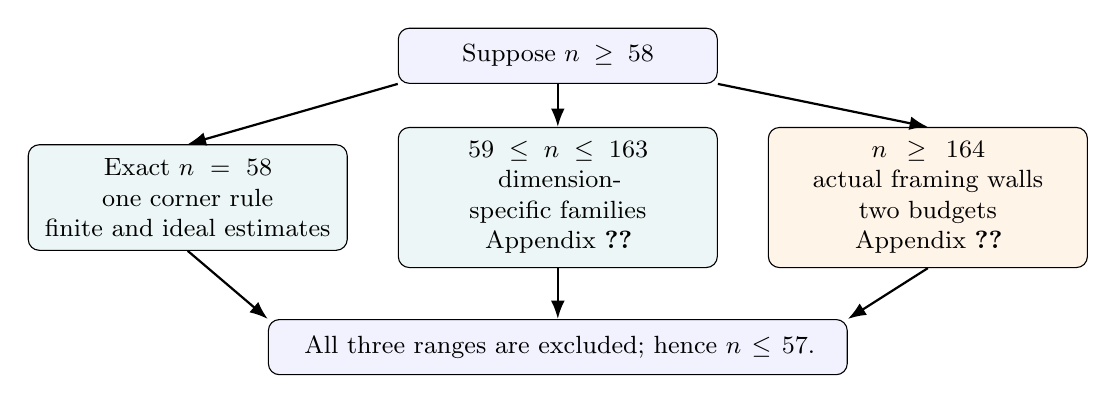
\begin{tikzpicture}[font=\small,>=Latex,
 box/.style={draw,rounded corners,align=center,text width=3.7cm,
 minimum height=1.25cm,inner sep=5pt}]
 \node[box,fill=blue!5,minimum height=.7cm] (start) at (6.6,3.8)
   {Suppose \(n\ge58\)};
 \node[box,fill=teal!7] (exact) at (1.9,2.0)
   {Exact \(n=58\)\\one corner rule\\finite and ideal estimates};
 \node[box,fill=teal!7] (bounded) at (6.6,2.0)
   {\(59\le n\le163\)\\dimension-specific families\\Appendix~\ref{fv:app:tail}};
 \node[box,fill=orange!9] (unbounded) at (11.3,2.0)
   {\(n\ge164\)\\actual framing walls\\two budgets\\Appendix~\ref{fv:app:narrow-tail}};
 \node[box,text width=7.0cm,minimum height=.7cm,fill=blue!5]
   (finish) at (6.6,.1)
   {All three ranges are excluded; hence \(n\le57\).};
 \draw[->,thick] (start.south west)--(exact.north);
 \draw[->,thick] (start)--(bounded);
 \draw[->,thick] (start.south east)--(unbounded.north);
 \draw[->,thick] (exact.south)--(finish.north west);
 \draw[->,thick] (bounded)--(finish);
 \draw[->,thick] (unbounded.south)--(finish.north east);
\end{tikzpicture}
\caption{The higher-dimensional exclusions, using the bounded
weight families and the narrow-facet argument.}
\label{fv:fig:ill20261026:fv57:tail}
\end{figure}
% END ILLUSTRATION_20261026_FV57_TAIL
\section{The bounded higher-dimensional tail}\label{fv:app:tail}

The purpose of this appendix is to state the mathematical objects behind
the higher-dimensional certificates. The rules change only at a small
number of ranks. Their shared comparison and algorithms are more useful
than the order in which those changes were discovered.

\subsection{The common comparison and terminal algorithm}

Put $d=n-1$ and
 \[
 \beta_n=\begin{cases}n(n-6)/8&n\text{ even},\\
 (n-1)(n-5)/8&n\text{ odd}.\end{cases}
\]
The incidence argument of Lemma~\ref{fv:lem:shape} applies at every rank:
\[
 \Dfive\ge\beta_n v_f+\sum_{v\ {\rm ideal}}\kappa(v)+\Delta_n,
 \qquad \Delta_n>0.
\]
The weaker bound $\Delta_n\ge5(n-1)$ suffices here. For a simultaneous
rule with finite bound $U_n$ and ideal charge $C(v)$, it is enough that
 $U_n\le\beta_n$ and $\kappa(v)-C(v)>0$ at every cusp. Subtraction as
in Lemma~\ref{fv:lem:payment-comparison} then gives a contradiction, even
if there are no ideal vertices.

For a cusp profile $\boldsymbol r=(r_1,\ldots,r_s)$ of total rank $d$,
define
 \[
 H_{\boldsymbol r}(t)=\prod_i(1+\cdots+t^{r_i})=\sum_jh_jt^j,\quad
 V_{\boldsymbol r}=\prod_i(r_i+1),\quad
 G_{\boldsymbol r}=\sum_jh_j\min(j,d-j).
\]
The normalized surplus associated with an affine-factor envelope $c$ is
 \begin{equation}\label{fv:eq:tail-margin}
 m_c(\boldsymbol r)=
 \frac{5G_{\boldsymbol r}-dV_{\boldsymbol r}}{2V_{\boldsymbol r}}
       -\sum_i c(r_i).
\end{equation}
The factor-fiber theorem gives
 $C(v)\le V_{\boldsymbol r}\sum_i c(r_i)$. This multiplicity is a
geometric statement; a graph pair count alone would not establish it.

Lemma~\ref{fv:lem:concentration} permits the move
 $(a,b)\mapsto(a-1,b+1)$, $1\le a\le b$, whenever
 $c(a-1)+c(b+1)\ge c(a)+c(b)$. The normalized curvature, and hence
\eqref{fv:eq:tail-margin}, does not increase. The product of the two
link vertex counts decreases, since
 $(a+1)(b+1)-a(b+2)=b-a+1>0$.
Every move raises the integer sum of squared ranks by
 $2(b-a+1)$, while that sum is at most $d^2$. Thus concentration halts.
A positive terminal margin extends to every original cusp. If an
absolute surplus is used, its normalized positivity is checked before
multiplying by the larger original vertex count.

The terminal enumeration is the sorted-partition recursion in
Section~\ref{fv:sec:ideal}, with the following additional multiplicity
conditions. For a linear/cap envelope $c(r)=\min(r/2,L/2)$, terminal
profiles have arbitrary copies of $L$, at most one part below $L$, and
at most one above $L$. For a low-only reduction, they have at most
one part below $L$ and arbitrary parts at least $L$; high parts are
not concentrated. In a piecewise rule the freely repeated ranks
are listed below, and each other named exceptional rank occurs at
most once. Adjoin each part only if these conditions survive.
The remaining rank decreases at every recursive call. The unique
first part of a sorted partition proves completeness and uniqueness.

For each profile compute $H$ by integer convolution and $V$ independently
by its product. Check the degree, symmetry and coefficient sum;
compute $G$ from its weighted sum and independently from cumulative
probabilities of the sum of uniforms. Then evaluate
\eqref{fv:eq:tail-margin} exactly. A certificate verifies equality of its
profile domain with this recursion, every coefficient identity and
every positive margin. An advertised minimum also carries an attaining
profile. These are finite algorithms with proved domains, not a
search for a favorable cusp decomposition.

Finite-vertex costs use the same typed-forest algorithm as
Appendix~\ref{fv:app:finite-contexts}. The fixed counts and residual
state retain every multiplicity or guard that affects a later charge.
All last-item inequalities are checked, and equality predecessors
are supplied whenever an exact maximum is asserted.

\subsection{The elementary families in dimensions98--163}

A feature is a node of degree at least three or an endpoint of a
nonsimple bond, including a parallel bond. Distances are graph
distances. A condition on a whole component always concerns the
whole actual endpoint diagram.

For $98\le n\le108$, finite weights are one at distance at most9
or in a whole component of order at most17. Their total is at most $9n$.
At a cusp, pay one at distance at most8, in a whole component of
order at most17, or at distance9 if a mark is within14 steps of
a feature. These are alternative conditions for one unit, not
separate charges. For an affine component of order $m\ge18$, the
exact counts are
 \[
 \begin{array}{c|c}
 A&8m\\ C&\min(9m-45,8m-4)\\
 B&\min(9m-44,8m-2)\\D&\min(9m-43,8m).
 \end{array}
\]
For example, a $C$ spine contributes $8m-36$ short pairs; the extra
distance-nine starts occupy the first16 and last16 available positions,
giving $\min(m-9,32)$. In $B$ the spine windows have lengths15 and16
and the leaves add two pairs. In $D$ both windows have length15 and
the leaves add four pairs. The union of the first $a$ and last $b$
positions in a list of length $h$ has size $\min(h,a+b)$; this also
covers overlapping windows. Thus these are all-rank counts.
Orders at most17 cost at most $\binom m2\le8m$, so
 $c(r)=\min(8,r/2)$.

For $k=9,\ldots,13$, use unit weights at distance at most $k$ or
in whole components of order at most17, at both finite and ideal
vertices. The finite bound is $kn$ and
 $c(r)=\min(k,r/2)$. For $k=14$ the distance condition alone suffices.
The complete local replacement theorem for these distance families
is the core-routing theorem of Appendix~\ref{fv:app:routing}, with the
corresponding retained short-path threshold. It includes overlapping
cores and arbitrary additional supporting whites. The affine graph
count does not prove that local theorem.

The terminal algorithm above, with $L=2k$, gives the following exact
positive minima over the indicated dimensions and their entire
terminal domains:
\[
\begin{array}{c|c|c|c}
n&U_n&c(r)&\min m_c\\ \hline
98\!:\!108&9n&\min(8,r/2)&112101/1419857\\
109\!:\!116&9n&\min(9,r/2)&45873/2476099\\
117\!:\!126&10n&\min(10,r/2)&145234/4084101\\
127\!:\!136&11n&\min(11,r/2)&40603/559682\\
137\!:\!146&12n&\min(12,r/2)&172096/1953125\\
147\!:\!156&13n&\min(13,r/2)&830407/9565938\\
157\!:\!163&14n&\min(14,r/2)&1476616/20511149
\end{array}
\]
In every row $\beta_n>U_n$. This proves the exclusion of 98--163.

\subsection{Labelled rules for dimensions66--97}

We give the marked rules, not just their component sums. The finite
supplement tables used here are lists of unordered node pairs. They
have a mathematical generation algorithm stated below.

Number an affine component of order $m$ as follows. Type $A$ is the
 $m$-cycle. Type $C$ is the path $0,\ldots,m-1$, with label4 on the
first and last bonds. Type $B$ has spine $0,\ldots,m-3$, its last bond
labelled4, and simple leaves $m-2,m-1$ at 0. Type $D$ has spine
 $0,\ldots,m-5$ and leaves $m-4,m-3$ at 0 and $m-2,m-1$ at $m-5$.
All other bonds are simple and all unlisted pairs are orthogonal.
Finite $A_r,B_r$ use the path $0,\ldots,r-1$, with only the last
 $B$ bond doubled; finite $D_r$ has spine $0,\ldots,r-3$ and leaves
 $r-2,r-1$ at $r-3$. Positions are zero-based.

Let $q_b$ pay one at distance at most $b$, or at distance
 $b+1,\ldots,9$ with a mark within $b$ of a feature. Let $P_b(m,X)$
be its preferred-image completion in affine type $X$, with the
validated removals described below. At all other marked pairs
the weight is zero. The small ideal tables are:
\[
\begin{array}{c|c|c|c}
n&\text{all pairs paid}&\text{exceptional tables}&\text{larger orders}\\\hline
92\!:\!97&m\le16&P_7(17,X)&q_7\\
87\!:\!91&m\le15&P_7(16,X),P_7(17,X)&q_7\\
81\!:\!86&m\le14&P_6(15,X),P_6(16,X),P_6(17,X)&q_6\\
78\!:\!80&m\le13&P_5(14,X),\ldots,P_5(17,X)&q_5 .
\end{array}
\]
The totals, in the order $A,B,C,D$, are
 \[
\begin{array}{c|rrrr}
P_7(17)&119&111&108&127\\P_7(16)&112&107&103&111\\
P_6(15)&90&100&95&96\\P_6(16)&96&107&103&111\\
P_6(17)&102&111&108&127\\
P_5(14)&70&87&84&82\\P_5(15)&75&100&95&96\\
P_5(16)&80&107&103&111\\P_5(17)&85&111&108&127 .
\end{array}
\]
These totals check the tables; they do not define their marked entries.

Write $R_9$ for unit finite weight at distance at most9 or whole
rank at most17. For81--97 add a half between any mark in a whole
component of rank at most4 and a mark in $D_{12},\ldots,D_{16}$ at
its fork center or short leaf, or in $A_{13},A_{15}$ at its middle.
The full cost is at most $9n$ for $n\le108$. This slightly enlarges
the earliest cross rules, preserving every local payment.

Write $R_8$ for unit weight at distance at most8, at distance9 with
a whole-component leaf mark, or in whole rank at most17. Let $F_8$
add a half between any mark in whole rank at most5 and a mark of
 $D_{11},\ldots,D_{16}$ at its fork center or short leaf, of
 $A_{13},A_{15}$ at its middle, or of $A_{17}$ at position5 or11.
Also add a half between an $A_4$ endpoint and the unique long-arm
neighbor of the $D_{13}$ fork center. Count each marked pair once.
The complete finite bound is $8n$ for $n\le80$.

For78--80 use $F_8$ enlarged from $R_8$ to $R_9$. The added nonleaf
distance-nine pairs number $r-11$ in a rank $r\ge18$ path and $r-12$
in $D_r$, at most $r$. Ranks at most17 already pay all pairs.
Thus its cost is at most $9n$. The $D_{11}$ and $A_{17}$ coupons
must be retained: the ideal-five cycle replacements can require them.
For76--77 use $F_8$ itself. For70--75 also upgrade the half for
 $A_1/D_{12}$ at a short leaf to1, and add a half for either $A_2$
mark paired with the short terminal of $B_{10}$ incident to its
doubled bond. The bound remains $8n$ for $n\le75$.

For69 additionally delete the finite $A_{17}$ endpoint pair,
upgrade $A_1/D_{11}$ short-leaf pairs to1, and pay1 for $A_1/A_{11}$
or $1/2$ for $A_2/A_{11}$ at the $A_{11}$ middle. Its finite maximum
at 69 is544. For67--68 replace the rank 17 same-component tables
by $T_{17}(A),T_{17}(B),T_{17}(D)$ of costs114,105,127 defined
below; the maxima become504,512. For66 also change short-leaf
distance-nine pairs in whole $D_r$, $r\ge20$, from1 to $1/2$,
add a half between whole rank at most5 and a short leaf of $D_{10}$,
and upgrade $A_2/D_{11}$ short-leaf halves to1. Its maximum is495.
All these are actual whole-component conditions. A representative
count may allow $B_{17}$ the larger $D_{17}$ cost127, but may not
identify the coupon-bearing $A_{17}$ with those types.

For the ideal weights below78 start with $P_5$ at orders14--17,
all pairs at orders at most13, and $q_5$ at orders at least18.
Apply the following setting operations for the listed dimensions:
\begin{center}\small
\begin{tabular}{p{.12\textwidth}p{.79\textwidth}}
\toprule$n$&Patch\\\midrule
66--77&$D$,order 17: set $(1,11)$ to0.\\
66--75&$B$,order 15: set $(0,11),(11,13),(11,14)$ to0.\\
66--74&Use the order 13 tables below; set $H_{17}$ to $1/2$.\\
66--71&$D$,order 16: set $H_{16}$ to $1/2$.\\
66--70&$B$,order 14: set $(0,10)$ to0; $B$,order 15: set $(1,11)$ to0.\\
66--69&Use the order 12 tables below.\\
66&$B$,order 12: set $(9,10),(9,11)$ to0; $C$,order 12:
set $(0,10),(1,11)$ to0; $B$,order 14: set $(10,12),(10,13)$ to0.\\
\bottomrule
\end{tabular}
\end{center}
Here
 \[
\begin{split}
H_{17}={}&\{(0,10),(2,12),(0,11),(1,12),(1,15),(1,16),\\
 & (11,13),(11,14),(2,15),(2,16),(10,13),(10,14)\},\\
H_{16}={}&\{(0,10),(1,11),(1,14),(1,15),(10,12),(10,13),\\
 & (2,14),(2,15),(9,12),(9,13)\}.
\end{split}
\]
At order 13 use cycle distance at most5 in $A$; all pairs except
 $(0,10),(10,11),(10,12)$ in $B$; all except
 $(0,10),(0,11),(0,12),(1,12),(2,12)$ in $C$; and all except
 $\{9,10\}\times\{11,12\}$ in $D$. The costs are65,75,73,74.
At order 12 use cycle distance at most5 in $A$; all pairs with
halves at $(9,10),(9,11)$ in $B$; all except $(0,11)$ in $C$;
and all except $\{8,9\}\times\{10,11\}$ in $D$.
The costs before the 66 patch are60,65,65,62 and after it
60,64,63,62. Orders at most11 remain wholly paid.
Each marked set is invariant under the labelled target's automorphisms;
equivalently apply it under every identification with that target.

\subsection{Finite-table generation and verification}

A preferred record consists of two labelled minimal cores, their
induced overlap, the two marked black pairs, the selected connected
corner component $J$, its two marks, and its proved whole-completion
order bound $h\le17$. Appendix~\ref{fv:app:routing} defines the admissible
core domain and its selected routes. For every record with $h\ge m$
and $|J|\le m$, enumerate all induced labelled injections into the
target of order $m$. Assign an unassigned pattern node and try every
unused target node having the correct labels to all nodes already
assigned, including zero labels. The recursion has depth at most17
and branching at most17. Each injection has a unique branch, so
induction proves termination, completeness and absence of missed
orientations. Take the union of marked images, not their multiplicity.

The table $P_b(m,X)$ is this union with $q_b$, followed by the
validated cycle removal above distance $b$ and, in the applicable $D$
targets, removal of
 \[
 \{p:\operatorname{dist}(p)\ge m-4\}
   \ \cup\ \{\text{the pair of degree-three nodes}\}.
\]
The latter has nine pairs. The finite supplement contains the labelled
pattern records and paid-set records $(b,m,X,P)$, where $P$ is a list
of distinct unordered pairs $0\le i<j<m$. Missing entries mean zero.
The preferred-image algorithm and the setting operations above
therefore specify the actual weights without executing an import.

The initial ideal-five domain has949 overlap records,571 with bound
at least14. The distance-eight domain has2614 records,1153 with
bound at least14; its entire marked image union lies in those same
paid or validated-removal sets. It changes no table. Ideal-six
uses437 eligible records; ideal-seven uses260 at order 16 and80
at order 17. These numbers are consistency checks, not completeness
proofs in place of the stated domains.

For $T_{17}$ take the union of $R_8$'s short/leaf-nine pairs, all
bound17 selected marked images, and all marked images whose retained
replacement is a unit in the complete literal-interface ledger.
Then delete the $A_{17}$ endpoint pair by its separate validated
transfer. It occurs in neither the basic nor the selected high-pattern
union; all literal totals are recounted after deletion. This finite
definition is stronger than merely recording the costs114,105,127.
Equivalently its complete literal description is the basic short/leaf-nine
set together with
 \[
\begin{array}{c|l}
A_{17}&(2,11),(2,12),(2,13),(2,14),(3,12),(3,13),\\
 &(3,14),(4,13),(4,14),(5,14),(0,13),(3,16)\\
B_{17}&(2,11),(3,12),(4,13),
\end{array}
\]
with unit weights, while $D_{17}$ pays every pair except
 \[
\begin{gathered}
(0,10),(0,11),(1,10),(1,11),(1,12),\\
(1,13),(1,14),(1,15),(1,16).
\end{gathered}
\]
This explicit alternative fixes every marked entry, including old zeros.

The supplement verifier reconstructs all target graphs and all induced
injections, compares the resulting pair sets, checks every patch
entry and automorphism image, and sums every actual component and
cross-role cost. It then checks the Bellman upper inequalities for
the complete typed forest domain. Its correctness is the preceding
union argument and induction on residual rank. Its halting follows
from the explicit order 17 target bound and the finite rank limit
of the particular interval. The geometric proof separately shows
that every removed preferred or literal image has a retained actual
replacement and that every added-white contact is covered; neither
the pair-list verifier nor the forest maximum proves that statement.

\subsection{Envelopes and recorded bounded calculations}

For ideal-five factors of order $m\ge18$, the all-rank counts are
 \[
\begin{split}
p_A(m)&=5m,\\
p_C(m)&=5m-15+\sum_{k=6}^{9}\min(m-k,14),\\
p_B(m)&=5m-6+\sum_{k=8}^{11}\min(m-k,13),\\
p_D(m)&=5m+3+\sum_{k=10}^{13}\min(m-k,12).
\end{split}
\]
The same initial/final-window argument used above proves these
formulas including overlap. Put $g(r)=\max_Xp_X(r+1)/(r+1)$.
Their five linear branches have slopes9,8,7,6,5 and give
 $g(r)\le163/23$, with equality at $r=22$, and
 $g(r)=(5r+56)/(r+1)$ for $r\ge24$.

For66--80 use $r/2$ through the stated low rank, the following
successive values up to rank 16, and the constant $163/23$ at
every rank at least17:
\[
\begin{array}{c|c|l}
n&\text{linear through}&\text{successive exceptional values}\\\hline
66&10&16/3,\ 75/13,\ 6,\ 32/5,\ 107/16,\ 120/17\\
67\!:\!69&10&65/12,\ 75/13,\ 43/7,\ 32/5,\ 107/16,\ 120/17\\
70&11&75/13,\ 43/7,\ 32/5,\ 107/16,\ 120/17\\
71&11&75/13,\ 87/14,\ 97/15,\ 107/16,\ 120/17\\
72\!:\!74&11&75/13,\ 87/14,\ 97/15,\ 111/16,\ 120/17\\
75&12&87/14,\ 97/15,\ 111/16,\ 126/17\\
76\!:\!77&12&87/14,\ 20/3,\ 111/16,\ 126/17\\
78\!:\!80&12&87/14,\ 20/3,\ 111/16,\ 127/17 .
\end{array}
\]
For81--86 the envelope is linear through 13, then
 $20/3,111/16,127/17$, then constant $95/13$. For87--91 it is
linear through 14, then $7,127/17$, then constant $217/29$.
For92--97 it is $\min(15/2,r/2)$.

The freely repeated terminal ranks are respectively
 \[
\begin{array}{c|l|l}
n&\text{repeated ranks}&\text{at most once}\\\hline
66&10,11,12,14,15,16,17&13;\ \text{one}<10,\ \text{one}>17\\
67\!:\!69&10,11,13,14,15,16,17&12;\ \text{one}<10,\ \text{one}>17\\
70\!:\!74&11,13,14,15,16,17&12;\ \text{one}<11,\ \text{one}>17\\
75\!:\!80&12,14,16,17&13,15;\ \text{one}<12,\ \text{one}>17\\
81\!:\!86&13,16,17&14,15;\ \text{one}<13,\ \text{one}>17\\
87\!:\!91&14,16,17&15;\ \text{one}<14,\ \text{one}>17 .
\end{array}
\]
The special moves $2j\mapsto(j-1,j+1)$ have cost gains
 $11/65$ at $j=13$ for66; $23/1092$ at $j=12$ for67--69;
$19/182$ at $j=12$ for70; $16/91$ at $j=12$ for71--74;
and at $j=13,15$, respectively,
$(4/105,7/2040)$ for75, $(5/21,83/408)$ for76--77,
and $(5/21,107/408)$ for78--80. For81--86 the gains at 14,15
are $5/48,107/408$; for87--91 the gain at 15 is $8/17$.
All are positive. The rank 12 duplicate move at 66 is deliberately
not used: its gain would be negative.

The recorded exact calculations are:
\[
\begin{array}{c|c|c}
n&U_n&\min m_c\\\hline
66&495&13367/495924\\
67\!:\!68&504,\ 512&851/165888\\
69&544&3641/13608\\70&8n&1819/51840\\
71&8n&23641/338688\\72\!:\!74&8n&6875/49152\\
75&8n&63/74698\\76\!:\!77&8n&11615/448188\\
78\!:\!80&9n&409611/2171546\\
81\!:\!86&9n&940675/11294304\\
87\!:\!91&9n&146417/911250\\
92\!:\!97&9n&10121/4194304 .
\end{array}
\]
For an interval the minimum is taken over all its dimensions and
all terminal profiles. The finite comparisons satisfy $U_n\le\beta_n$.
Consequently the single comparison at the start of the appendix
excludes66--97.

\subsection{The complete ambient59--65 layer table}
\label{fv:app:early-tail}

Write $R_N$ for the rule used at ambient dimension $N$. Starting from
the literal ambient66 rule above, apply the following assignments in
the order 65 down to59. An assignment \emph{sets} a weight; it is not
a repeated debit. Other entries inherit. In the cross table later
rows replace earlier ones, not add to them. There are no context
guards until $R_{59}$. Put
 $E_r=\{0,r-1\}$ and $P_k(A_r)=\{k-1,r-k\}$.

Finite features in this subsection include endpoints, branch nodes
and endpoints of nonsimple bonds in the whole component. Let $\delta$
be distance to this set. Outside the small-rank overrides below,
the complete changes to the basic distance rule are
 \[
\begin{array}{c|ccc}
N&\text{distance6}&\text{distance7}&\text{distance8}\\\hline
65&\text{unchanged}&\text{unchanged}&1/2\ \text{if both depths}\ge17\\
64,63,62&\text{unchanged}&\text{unchanged}&0\ \text{if both depths}\ge11\\
61&\text{unchanged}&\text{unchanged}&0\ \text{if both depths}\ge8\\
60&\text{unchanged}&0\ \text{if both depths}\ge6&0\ \text{if both depths}\ge8\\
59&0\ \text{if both depths}\ge6&0\ \text{if both depths}\ge6&
 0\ \text{if both depths}\ge8 .
\end{array}
\]
In particular the ambient59 distance-eight depth is8, not the
depth-six value of the final ambient58 rule.

The finite supplement has complete tables
 $\mathsf F_{N,X,r}$, keyed by ambient layer, finite type and rank.
They are lists of records $(i,j,w_{ij})$ with $0\le i<j<r$ and exact
rational weights; absent pairs mean zero. A retained-pair list
instead means its unit indicator. A changed-pair list is only a
patch, never a full table. Target graphs and all their zero labels
must agree with the canonical labels. These are finite mathematical
arrays, with exact selectors specified in the supplement receipt;
one does not call a producer to evaluate a corner. The following
assignments either print the full patch or name a complete
 $\mathsf F$ table.

At65 set $A_{16}$ pairs $(0,14),(0,15),(1,14),(1,15)$ to zero.
Set to zero in $B_{16}$
\[
\begin{split}
 &(0,11),(0,12),(0,13),(0,14),(0,15),
 (1,12),(1,13),(1,14),(1,15),\\
 &(2,13),(2,14),(2,15),(3,14),(3,15),(4,15),(5,15).
\end{split}
\]
Halve $D_{16}$ pairs $(1,12),(1,13),(1,14),(1,15)$ and $D_{17}$
pairs $(2,13),(2,14),(2,15),(2,16)$. Their costs are
 $A_{16}/B_{16}/D_{16}=116/104/118$ and
 $A_{17}/B_{17}/D_{17}=114/105/125$.
At64 set $D_{16}(0,11),(0,12)$ to zero and restore
 $D_{17}(1,12),(1,13)$ to one.
At63 set to zero
 $A_{16}(0,12),(3,15)$,
$D_{16}(0,10),(0,13)$ and
 $D_{17}(1,12),(1,13)$.

At62 halve $A_{15}(0,13),(1,14)$ and $D_{15}(0,13),(0,14)$,
delete $B_{15}(0,14)$, halve $A_{16}(0,11),(4,15)$ and
 $D_{16}(2,13),(2,14),(2,15)$, and set
 $A_{17}(1,12),(4,15)$ to halves.
In $D_{17}$ set $(0,12),(0,13)$ to zero and
 $(0,14),(0,15),(0,16),(4,14),(4,15),(4,16)$ to halves.

At61 replace the finite tables for
 $A_{15},B_{15},D_{15},A_{16},D_{16},D_{17}$ by their complete
 $\mathsf F_{61,X,r}$ arrays; all earlier zeros and halves remain
part of those arrays. At60 replace the three rank 15 arrays by
 $\mathsf F_{60,X,15}$. For $A_{16},A_{17}$ take the complete
full-payment exchange arrays and set respectively
 $(0,11),(4,15)$ to $1/8$ and $(1,12),(4,15)$ to $7/8$.
For $D_{16},D_{17}$ take the complete eighth-balance arrays and set
respectively $(0,14),(0,15)$ to $7/8$ and $(1,15),(1,16)$ to $1/8$.
These setting operations, not the arrays' earlier $5/8,3/8$
versions, define $\mathsf F_{60}$.

At59 use complete $\mathsf F_{59}$ arrays for all three rank 14
types,$A_{15},D_{15},D_{16},A_{17}$. Relative to $R_{60}$, set
 $D_{17}(2,12)$ to $5/8$, $(2,14)$ to0, and $(3,15),(3,16)$ to0.
The two disjoint $D_{17}$ patches are accumulated; their separate
earlier whole arrays must not overwrite each other.
The base costs, useful for checking these full marked arrays, are
 \[
\begin{array}{c|rrrrrr}
N&A_{15}&B_{15}&D_{15}&A_{16}&D_{16}&D_{17}\\\hline
62&104&104&104&113&225/2&120\\
61&103&103&103&111&111&119\\
60&101&97&201/2&441/4&443/4&467/4\\
59&100&97&100&441/4&439/4&919/8 .
\end{array}
\]
At59 the rank 14 costs are $89,87,181/2$ in $A,B,D$, and the $A_{17}$
cost is $451/4$. These sums do not define the marked entries.

Here is the entire accumulated ordinary cross-role update table.
Every component named is whole; a small rank-five allowance includes
all irreducible types where the broad rule allows them. An entry
with a product of mark sets applies to every pair in that product.
All unlisted entries remain their earlier values.
{\small
\begin{longtable}{r p{.28\textwidth}p{.39\textwidth}r}
\toprule$N$&First marked component&Second marked component&Weight\\\midrule
\endhead
65&$A_1$ or $A_2$, all&$D_{14}$,node10&$1/2$\\
64&$E_6$,long ends&$D_{11}$,short leaves&$1/2$\\
64&$A_1$&$B_{10}$,terminal9&$1/2$\\
63&$A_4,E_4$&$A_{12},E_{12}$&1\\
63&$A_4,E_4$&$A_{13},P_2$&1\\
63&$D_5$,long0&$A_{12},P_2$&1\\
63&$A_2$,all&$A_{13},E_{13}$&$1/2$\\
63&$A_2$,all&$A_{14},P_2$&$1/2$\\
63&$E_6$,long ends&$A_{11},P_2$&1\\
63&$A_2$,all&$B_9$,terminal8&$1/2$\\
63&$A_2$,all, or $A_3$,middle1&$D_{10}$,center7&$1/2$\\
62&$A_2$,all, or $A_3$,middle1&$D_{10}$,center7&1\\
62&$E_6$,long ends&$D_{11}$,short leaves&1\\
61&$A_2$,all&$A_{13},E_{13}$&1\\
61&$A_1$&$A_{13},E_{13}$&$1/2$\\
61&$A_2$,all&$A_{14},P_3$&$1/2$\\
61&$A_4,E_4$&$A_{12},P_3$&$1/2$\\
61&$A_1$&$B_{10}$,terminal9&1\\
60&$A_2$,all&$D_{13}$,short leaves&1\\
60&$A_4,E_4$, or $A_5,P_2$&$D_{11}$,short leaves&1\\
60&$D_5$,short leaves3,4&$D_{12}$,center9 or leaves10,11&1\\
60&$D_5$,long0&$D_{12}$,short leaves10,11&$7/8$\\
60&$D_5$,long0&$A_{11},P_2$&1\\
60&$A_4,E_4$&$B_9$,terminal8&$1/2$\\
60&$D_5$,long0&$D_{11}$,short leaves9,10&1\\
60&$A_1$&$B_{11}$,node9&$1/2$\\
60&all marks, any rank 2--5 component&$D_{16}$,center13 or leaves14,15&0\\
59&$A_2$,all&$A_{13}$,middle6&$7/16$\\
59&$A_2$,all&$D_{13}$,center10&$7/16$\\
59&$A_1$&$A_{13}$,middle6&$9/16$\\
59&$A_1$&$D_{13}$,node9&$1/2$\\
59&$D_5$,long0&$D_{12}$,short leaves10,11&$1/2$\\
59&$D_5$,long0&$A_{12},E_{12}$&$3/8$\\
59&$A_1$&$D_5$,long0&$3/8$\\
59&$D_5$,short leaves3,4&$A_{12},P_3$&1\\
59&$A_1$&$A_{14},P_3\cup P_4$&$1/2$\\
59&$A_1$&$A_{15},P_3$ or $A_{16},P_4$&$1/2$\\
59&$A_1$&$D_{14}$,node9 or $D_{15}$,node11&$1/16$\\
59&$A_1$&$A_{12}$,nodes5,6&1\\
59&$A_1$&$B_{12}$,node9&$1/2$\\
59&$A_1$&$A_{12},E_{12}$ or $A_{13},P_2$&$1/4$\\
59&$A_4$,internal1,2&$A_{13},P_2$&$1/2$\\
59&$A_4,E_4$&$A_{11},E_{11}$&$1/2$\\
\bottomrule
\end{longtable}
}
The $D_5$ long-end/$D_{12}$ center remains its broad half:
the $7/8$ at 60, and its replacement half at 59, concern only the
short $D_{12}$ leaves. The full $D_5/D_{12}$ costs are therefore
 $45/4$ and $21/2$. The $D_5/D_{11}$ cost is $17/2$ and the $D_5/A_{11}$
cost is2. These distinctions matter to which actual corner can pay.
The 59$A_1/D_5$ entry is unconditional; the later58 guards are not
imported. There is no $A_1/A_{16}$ endpoint quarter here, and the
 $A_4/A_{12}$ third-node value at 59 is still a half.

At59 add exactly two Boolean context roles: a marked pair in two
distinct $A_2$ components receives $1/8$ if an unmarked $A_{10}$ and
two unmarked $A_1$ components are present; an $A_2$ mark paired with
the $D_5$ long end receives $1/2$ if unmarked $A_1,A_9$ components
are present. Multiple witnesses do not multiply a payment. Their
forest totals are
 \[
 \tfrac14a_2(a_2-1)[a_1\ge2,\ a_{10}>0]
       +a_2d_5[a_1>0,\ a_9>0].
\]
There are no other context terms, in particular no rank 15-presence
same-component guards.

For ideal vertices introduce complete supplement arrays
 $\mathsf I_{N,m,X}$ with the same pair schema and zero default.
At65 use the order 12--17 arrays of the short-seven small-factor
interface. This is a replacement, not the assumption that the
older66 order 15 tables already agree. Orders at most11 are all
unit, orders at least18 use $q_5$. At64 halve order 11 cycle
distance-five pairs, $B$ pairs $(8,9),(8,10)$, the $C$ endpoint
pair $(0,10)$, and $D$ pairs $\{7,8\}\times\{9,10\}$;
also halve $D$,order 17,$(3,15),(3,16),(9,13),(9,14)$.
At63 set $C$,order 11,$(0,10)$ to zero; $B$,order 12,$(0,9)$
to zero; and $D$,order 13,$(0,8)$ to a half.
At62 set that last pair to zero, set $B$,order 16,$(1,11),(2,12)$
to zero, delete the four just-halved order 17$D$ pairs, and set
 $B$,order 14,$(9,12),(9,13)$ and $C$,order 14,$(1,12)$ to zero.
At61 set $B$,order 11,$(8,9),(8,10)$ and $C$,order 11,
$(0,9),(1,10)$ to zero, and set $D$,order 16,$(0,9),(2,11)$
to halves.

At60 use complete $\mathsf I_{60}$ tables for the type/order pairs
 \[
\begin{gathered}
(B,12),(C,12),(B,13),(C,13),(D,13),(C,14),\\
(B,15),(D,15),(B,16),(D,16),(D,17).
\end{gathered}
\]
The order 17$D$ table is the final rebalance table: its two center
pairs $(0,10),(2,12)$ are restored to halves, and
 $(2,15),(2,16),(10,13),(10,14)$ have weight $1/8$.
At59 use complete $\mathsf I_{59}$ replacements for
 \[
\begin{gathered}
(B,13),(C,13),(B,14),(C,14),(D,14),\\
(B,15),(D,15),(C,16),(D,16),(D,17).
\end{gathered}
\]
Equivalently the latter ideal rule is precisely the intrinsic58
table of Appendix~\ref{fv:app:weights}, except that every order 10
pair has weight1. This is checked against the complete snapshots,
not inferred from family totals. Orders at most10 remain wholly
unit throughout59--65 and orders at least18 keep $q_5$.

The full finite and ideal arrays above are retained mathematical
supplement tables, not descriptions by component cost. Their receipt
keys specify type, order/rank and canonical labelled graph, with all
edges and nonedges checked. Each finite snapshot is a complete
pair-domain replacement, or is followed by the explicitly printed
patch. Each array is bound by the corresponding immutable
composition's source manifest. The supplement verifier selects by
these keys, reads exact rational records, checks the pair domain and
default, and applies the stated setting operations. All loops have
at most $\binom{17}{2}$ entries per small table, and there are seven
layers; hence evaluation halts and determines every marked weight.
It is distinct from the proof that an actual face reaches those
marked roles.

For reference the small-affine family maxima at orders10--17 are
 \[
\begin{array}{c|rrrrrrrr}
N&10&11&12&13&14&15&16&17\\\hline
65&45&55&64&74&84&94&107&119\\
64&45&109/2&64&74&84&94&107&118\\
63&45&54&63&147/2&84&94&107&118\\
62&45&54&63&73&83&94&106&116\\
61&45&53&63&73&83&94&105&116\\
60&45&53&62&145/2&82&92&103&229/2\\
59&45&53&62&143/2&80&367/4&411/4&227/2 .
\end{array}
\]
Divide an entry by its order to obtain $c(r)$ at rank $r=m-1$.
For59--62 use the exact $g(r)$ above rank 16, with low-nine-only
concentration. For63--65 use the constant $163/23$ above rank 16;
the freely repeated ranks are9--17 at 63,64 and10--17 at 65,
with one lower and one higher part. The earlier all-rank formula
gives the remaining entries.
The exact arithmetic interface is
 \[
\begin{array}{c|r|c|c}
n&U_n&\min m_c&\min V m_c\\\hline
59&783/2&1/340&91/2\\
60&404&31/6000&54\\
61&420&3/250&64\\
62&434&2741/371712&73\\
63&449&3505/201344&139/46\\
64&464&2385/146432&240/23\\
65&479&61/1936&445/23 .
\end{array}
\]
All $U_n\le\beta_n$, so the common comparison excludes59--65.
The local proof uses the same core domain, arbitrary-support seals
and actual-corner priorities as Appendix~\ref{fv:app:routing}, but with
each layer's own marked table. Every newly reduced affine corner,
including a nonzero fractional reduction, is handled by its
whole-face theorem first. If the actual face has no such corner,
its ideal weights agree pointwise with the preceding layer.
Finite sparse changes then use their
distinct retained whole-component alternatives. Deep corridors use
the independent shorter-path route and preserve its feature and leaf
outputs. Guards are justified by physical whole-component seals
before entering the finite-state count. Thus no final58 restoration
or extra coupon is spent in an earlier tail rule.

\section{The unbounded tail: actual framing walls and two budgets}
\label{fv:app:narrow-tail}

The range $n\ge164$ requires a proof at all ranks, not a finite list
of partitions. We use Nikulin's narrow-facet theorem
\cite[pp.~654--655]{Nikulin}; its unrestricted statement is also given
in \cite[Section~4, p.~10]{NikulinNarrow}. A finite-volume chamber has a facet $F$
whose actual framing hyperplanes have pairwise distance strictly
less than $\operatorname{arccosh}7$. With outward normals of square2
this implies
 \begin{equation}\label{fv:eq:narrow}
 -(x,y)<14
\end{equation}
for any two framing walls. This is the external narrowness input.
We prove the incidence, endpoint and scale statements needed to
apply it; they are not additional hypotheses on the cusp.

\subsection{Outgoing edges really give framing walls}

Suppose first that $F$ contains a cusp $v$. Its horospherical link is
a product of affine Coxeter simplices. Write their ranks $r_a$,
with $\sum_ar_a=N=n-1$, and normalize every old root to square2.
In each factor choose two omitted nodes in advance. In the factor
containing the normal $\alpha_s$ of $F$, both choices avoid $s$.
The two choices need not be distinct. If that factor has affine rank
one, use its other node twice; its modified target $2(r_a-1)/9$ is zero.
Deleting one node per factor gives a positive-definite support $S$
of $N$ roots and a vertex of the horospherical link. It therefore
defines an actual outgoing edge in $F$. Finite volume gives a
finite or ideal second endpoint.

At a finite endpoint choose any new wall $x$ terminating that edge.
It and $\alpha_s$ belong to a spherical diagram, so their rank-two
Gram is positive definite. At an ideal endpoint let $T_b$ be its
affine factors. The positive-definite support $S$ contains at most
 $\operatorname{rank}T_b$ nodes from each. The total rank $N$ forces
equality in every factor: exactly one node of each $T_b$ is missing.
If the factor containing $\alpha_s$ has rank at least2, choose its
missing node as $x$; every pair in such a factor has finite angle.
If it is affine $A_1$, choose the missing node of another factor,
which is orthogonal to $\alpha_s$. Another factor exists in the
range at issue. Thus again the pair is positive definite.

To see that this is an actual ridge, start with a strict interior
timelike point $z$. Project it off the span of $x,\alpha_s$.
The projection correction is a nonnegative combination of those
normals, because their Gram is a positive-definite matrix with
nonpositive off-diagonal entries and nonnegative inverse.
Every other wall inequality stays strict, and the projected square
is even more negative. It gives a point of precisely their common
face. Hence $x$ is in the framing set controlled by
\eqref{fv:eq:narrow}. Apply the same construction to the second
omission tuple and call its terminating wall $y$.

Neither $x$ nor $y$ is an old deleted cusp wall: that wall is strict
along the outgoing edge away from $v$. Their old contact rows
 $p_j=-(x,\alpha_j)$ and $q_j=-(y,\alpha_j)$ are nonnegative,
and every nonzero entry is at least1. For each affine factor let
 $c_a=\sum_j\delta_{aj}\alpha_j$, with $\delta_{aj}>0$ normalized
by $\min_j\delta_{aj}=1$. These are nonzero future null vectors,
since their pairing with an interior point is negative. They are
all positive multiples $k_ac$ of one cusp vector $c$. Therefore
 \[
 \sigma_a=\delta_a\cdot p=-(x,c_a),\quad
 \tau_a=\delta_a\cdot q=-(y,c_a),\quad
 q_0=\sigma_a/\tau_a
\]
have a common positive ratio. Indeed, if a row height vanished,
all its nonnegative contacts with that factor would vanish;
proportionality of the $c_a$ would force every factor height and
every old contact to vanish. A square-two normal would then lie
in the null orthogonal complement of the full cusp span, impossible.

For each endpoint the principal Gram $S+x$ or $S+y$ is positive
semidefinite. Its Schur complement gives the separate budgets
 \begin{equation}\label{fv:eq:two-budgets}
 \sum_aC_{0a}\le2,\qquad\sum_aC_{1a}\le2,\qquad
 C_{\ell a}=p_{\ell,S_a}^{\,t}G(S_a)^{-1}p_{\ell,S_a}.
\end{equation}
The inverse is entrywise nonnegative. No bound on a deleted-node
contact or on its Coxeter label has been used.

\subsection{The common-height Lorentz identity}

Choose a null partner $d_0$ with $(c,d_0)=-1$, and write
 $x=a c+b d_0+u$, $y=a'c+b'd_0+u'$ in the orthogonal Euclidean
quotient. Then $b=-(x,c)>0$, $b'=-(y,c)>0$. Since
 $(x/b-y/b')\perp c$ and $x^2=y^2=2$,
\[
 \left\|u/b-u'/b'\right\|^2
   =2/b^2+2/(b')^2-2(x,y)/(bb').
\]
The quotient is the orthogonal sum of the affine factor spaces.
In factor $a$ put
 $E_a=\|u_a/\sigma_a-u'_a/\tau_a\|^2$.
Since $\sigma_a=k_ab$ and $\tau_a=k_ab'$, the $k_a^2$ cancels and
the preceding identity becomes
 \begin{equation}\label{fv:eq:lorentz-product}
 -(x,y)=\frac12\sum_a\sigma_a\tau_aE_a-q_0-q_0^{-1}.
\end{equation}
This proves the scale cancellation for a product cusp; no
commensurability or chosen horosphere is required.
Let $M=\max(q_0,q_0^{-1})$ and
 $W_a=\min(\sigma_a,\tau_a)^2E_a$. Then
 $\sigma_a\tau_aE_a=MW_a$ and $q_0+q_0^{-1}\le2M$.

The prescribed omission choices have targets
 \[
 T_a=2r_a/9\quad\hbox{ordinarily},\qquad
 T_a=2(r_a-1)/9\quad\hbox{in the sole avoid-node factor}.
\]
Thus $\sum T_a=(2N-2)/9$. We next prove
 \begin{equation}\label{fv:eq:two-range}
 \sum_aW_a\ge
 \begin{cases}(2N-2)/9-4&1\le M\le21/20,\\
 (2N-2)/9-16/3&M\ge21/20.
 \end{cases}
\end{equation}
It follows from\eqref{fv:eq:lorentz-product} that
 $-(x,y)\ge M(N-37)/9$ in the first range and
 $-(x,y)\ge M(N-43)/9$ in the second. At $N=163+t$ these are at
least $14+t/9$ and $14+7t/60$, respectively. They contradict
\eqref{fv:eq:narrow} for every $t\ge0$.

\subsection{Point potentials and the complete local domain}

For $r$ Euclidean coordinates put $s_k=e_1+\cdots+e_k$. The
classical point potentials and normalized kernel squares are
 \[
\begin{array}{c|l|l}
 &v_k&(\delta_k^2)\\\hline
B&v_0=0,\ v_1=e_1,\ v_k=s_k/2\ (k\ge2)&(1,1,4,\ldots,4,2)\\
C&v_k=s_k,\ \text{metric one half the usual metric}&(1,2,\ldots,2,1)\\
D&v_0=0,\ v_1=e_1,\ v_k=s_k/2\ (2\le k\le r-2)&\\[-2pt]
 &v_{r-1}=(s_{r-1}-e_r)/2,\ v_r=s_r/2&(1,1,4,\ldots,4,1,1).
\end{array}
\]
Write $R(i,j)=\|v_i-v_j\|^2$. For an $A$ cycle of order $m$ use
 $\delta=1$ and $R(i,j)=h(m-h)/m$, $h=(i-j)\bmod m$.
Ordinary omissions are $(0,\lfloor m/2\rfloor)$ in $A$ and
 $(0,r)$ in $B,C,D$. Modified $B,C$ use $(r-1,0)$ and $(1,r)$.
Rotations and fork automorphisms avoid a prescribed node in
 $A,D$ without weakening the ordinary geometric estimate.

Exceptional diagrams use the central node0 and consecutive labels
along arms $(2,2,2)$, $(1,3,3)$, $(1,2,5)$ for affine $E_6,E_7,E_8$.
Their rational symmetric matrices have diagonal2 and edge $-1$.
For $F_4$ use diagonal $(2,2,2,4,4)$, successive edges
 $(-1,-1,-2,-2)$ and scales $(1,1,1,2,2)$; for $G_2$ use
 \[
 A=\begin{pmatrix}2&-1&0\\-1&2&-3\\0&-3&6\end{pmatrix},
 \qquad(s_i)=(1,1,3).
\]
The physical Gram is $A_{ij}/\sqrt{s_is_j}$. If $k>0$ spans
 $\ker A$, put $\delta_i^2=s_ik_i^2/\min_j(s_jk_j^2)$.
Ground node0 and solve $Au=f$, $u_0=0$, for
 $f=e_i/k_i-e_j/k_j$; then
 $R(i,j)=\min_l(s_lk_l^2)f^tu$. This defines every resistance
by finite rational linear algebra.

Ordinary exceptional omissions are
 $E_6:(2,4)$, $E_7:(3,6)$, $E_8:(1,6)$,
$F_4:(0,4)$, $G_2:(0,2)$. To avoid $f$, take the first two
of $(2,4,6)\setminus\{f\}$ in $E_6$;
$(2,5)$ if $f\in\{4,7\}$ and $(4,7)$ otherwise in $E_7$;
$(1,6)$ if $f\in\{3,7\}$ and $(3,7)$ otherwise in $E_8$;
$(0,4)$ if $f\in\{1,3\}$ and $(1,3)$ otherwise in $F_4$;
and the other two nodes in $G_2$.
Modified $B_2$ has matrix
 $\left(\begin{smallmatrix}2&0&-2\\0&2&-2\\-2&-2&4\end{smallmatrix}\right)$,
scales $(1,1,2)$ and omissions $(0,1)$, avoiding node2.

The next enumeration is for the \emph{residual} product after a
failing factor has been selected below. Its ordered
budgets are at most $3/2$ on each side. The original product still
has budgets2; the failing-factor classification below is established
separately and does not apply this residual cap to the selected factor.
For the near range let $B=21/20$. The finite model list consists
of $A$ ranks1--16, $B,C$ ranks2--7, $D$ ranks4--17, all the
ordinary and avoid-node exceptional cases, modified $B$ ranks3--7,
modified $C$ ranks2--7, and modified $B_2$. For an omission $o$ a
retained contact $k$ is eligible only if $\delta_k^2R(o,k)\le3/2$.
Enumerate every subset $S$ of these nodes and retain it only if
 \begin{equation}\label{fv:eq:tail-support-cost}
 c_o(S)=\sum_{k\in S}\delta_k^2R(o,k)
 +\sum_{k<l\in S}\delta_k\delta_l
       [R(o,k)+R(o,l)-R(k,l)]\le3/2 .
\end{equation}
The retained inverse is nonnegative, so this is a lower bound for
every row with that support and magnitudes at least1.
Include or omit the omitted-node contact independently on each
side; included means magnitude at least1. Each full row is nonempty.
The two-empty-retained case has the direct bound $W\ge T$.

For full supports $U,V$, their normalized potentials lie in two
finite convex hulls. Form their positive-semidefinite signed
point Gram $K$ and the two row-sum constraints $Az=(1,1)$, $z\ge0$.
An exact lower-distance certificate consists of
 \[
 Az=(1,1),\quad Kz+A^t\lambda\ge0,\quad
 z_i(Kz+A^t\lambda)_i=0,\quad
 e=z^tKz=-\lambda_1-\lambda_2.
\]
Expanding the quadratic at $z$ proves that $e$ is the global minimum
on the two hulls. Enumerate active subsets and solve their rational
KKT equations; verify a witness by these identities. Exhaustion
always halts; failure to find a witness is a failed certificate,
never an omitted support.

Singular active systems may be skipped for the following reason.
Choose a minimum on the product of the two simplices having the
fewest positive coordinates, and restrict to that support $I$.
Both side-sum constraints are nonempty and independent. If its
bordered KKT matrix were singular, a nonzero null pair $(h,\nu)$
would satisfy
 \[
 A_Ih=0,\qquad K_Ih+A_I^t\nu=0.
\]
Multiplying by $h$ gives $h^tK_Ih=0$. Positive semidefiniteness
implies $K_Ih=0$, and full row rank then gives $\nu=0$.
Thus $h\ne0$ and preserves both sums. Moving along $h$ until a
positive coordinate first reaches zero preserves feasibility and
the minimum, contradicting the choice of support. Some minimizing
active system is therefore nonsingular. Its rational solution is
found by the exhaustive search. This argument proves search
completeness; the displayed slack identities independently prove
soundness of each supplied certificate.

Writing $s=\sum_U\delta_k$, $t=\sum_V\delta_k$, the positive row
magnitudes and common ratio bound give
 \begin{equation}\label{fv:eq:height-envelope}
 W\ge \max\{\min(s,t)^2,\max(s,t)^2/B^2\}\,e .
\end{equation}
This covers arbitrary unbounded contact magnitudes by convex
normalization, not a finite angle list.

The saved exact calculation has91 finite models,1116 retained
support pairs,3630 nonempty continuous domains and1395 positive
losses. Radicals in support rejection and height bounds are rounded
outward to rational bounds with squared inequalities; every surviving
support cost is also checked exactly. The counts are checksums.
Coverage comes from the complete model list, all subsets and both
omitted-node states.

The remaining ranks have no positive loss. For $B$ ordinary $r\ge8$
the eligible retained sets are $\{1\},\{r-1\}$; for modified $B$ they
are $\{r-2,r\},\{1\}$. The energy lower bounds are $(r-2)/4$ and
 $(r-3)/4$, with height-square at least $2/B^2$.
For ordinary $C$ they are $\{1\},\{r-1\}$, and for modified $C$,
$\{0,2\},\{r-1\}$; energy is at least $(r-2)/2$ and $(r-3)/2$,
with height-square at least1. For $D$, $r\ge18$, the sets are
 $\{1\},\{r-1\}$ and energy is at least $(r-2)/4$ with height-square1.
Omitted-node contacts may also occur. Each difference of full
convex-hull points has the indicated fixed middle coordinates,
of magnitude $1/2$ in $B,D$ or1 in $C$. Their number proves the
energy bounds. Subtracting $T$ gives a nonnegative constant at the
initial rank and a positive coefficient of the excess rank.

For an $A$ cycle, $m\ge18$ even or $m\ge19$ odd, cost at most $3/2$
permits only one adjacent retained node per side. Singleton full
supports have separation at least $\lfloor m/2\rfloor-2$;
the margin numerator is
 $m^2+8m-9(4+\varepsilon)^2$ over $36m$.
If a full row has two nodes, its height is at least $2/B$ and the
margin numerator is
 $(9-2B^2)m^2+(2B^2-72)m-81\varepsilon$ over $9B^2m$.
Here $\varepsilon=m\bmod2$. Substituting $m=18+2u$ or $19+2u$,
$u\ge0$, gives nonnegative coefficients and a positive constant.
This proves the tails at every rank.

\subsection{The classical unit-charge estimate at the original budgets}
\label{fv:app:full-budget-classical}

The residual calculation above starts only after a failing factor has
been selected. To justify that selection, we first need a statement at
the original endpoint budgets. In this subsection each retained row has
cost at most two; neither row is restricted to the residual budget
 $3/2$.

\begin{lemma}[Full-budget classical unit charge]
\label{fv:lem:full-budget-classical-unit}
For the prescribed ordinary or avoid-node omissions of a classical
affine factor, let $C_0,C_1\le2$ be its actual retained costs, and let
 $W=\min(\sigma,\tau)^2E$. If the common height ratio is at most
 $B=21/20$, then
 \[
 W+C_0+C_1\ge T,
\]
where $T=2r/9$ ordinarily and $T=2(r-1)/9$ in an avoid-node factor.
This includes arbitrary real contact magnitudes with every nonzero
contact at least one, and both possibilities for each omitted-node
contact.
\end{lemma}

\begin{proof}
The point potentials and kernel squares are those already displayed
above. For omissions $i,j$, put
 \[
 R=R(i,j),\qquad
 c_{ik}=\delta_k^2R(i,k),\qquad
 \ell_{ik}=R(i,j)+R(i,k)-R(k,j).
\]
The number $c_{ik}$ is the unit-contact inverse diagonal, not the
actual cost of an arbitrary contact. Normalizing a full contact row by
its affine height gives nonnegative convex weights $w_k$, of sum one.
The omitted node itself is allowed in this convex combination; its
displacement and its linear loss are zero. Write the two normalized
point means as $v_i+a,v_j+b$. Direct polarization gives
 \begin{equation}\label{fv:eq:full-budget-polarization}
 E=R-\sum_k w_k\ell_{ik}-\sum_l z_l\ell_{jl}
       +\|a-b\|^2.
\end{equation}
Every row height is at least one, so $W\ge E$. The positive retained
inverse and the contact gap give
 \[
 C_0\ge\sum_{k\text{ retained, contacted}}c_{ik},
 \qquad
 C_1\ge\sum_{l\text{ retained, contacted}}c_{jl}.
\]
Here all same-row cross terms are nonnegative. In particular, since
 $0\le w_k,z_l\le1$, a bound on each unit diagonal controls the
corresponding weighted linear losses without any upper bound on a
contact magnitude.

For $B,C,D$ the following table is the complete contact partition.
An asterisk denotes the prescribed avoid-node omissions. The column
``trivial'' marks a contact for which $c_{ik}>T$; if such a contact is
present, $C_0+C_1>T$ already proves the assertion. In every other row
 $\ell_{ik}\le c_{ik}$.

{\small
\begin{longtable}{@{}llllll@{}}
\toprule Type&$(i,j)$&retained $k$&$c_{ik}$&$\ell_{ik}$&trivial\\\midrule
\endhead
$B$&$(0,r)$&$1$&$1$&$1$&\\
$B$&$(0,r)$&$2\le k\le r-1$&$k$&$k/2$&\\
$B$&$(0,r)$&$r$&$r/2$&$r/2$&\\
$B$&$(r,0)$&$0$&$r/4$&$r/2$&yes\\
$B$&$(r,0)$&$1$&$r/4$&$r/2-1$&yes\\
$B$&$(r,0)$&$2\le k\le r-1$&$r-k$&$(r-k)/2$&\\
$B^*$&$(r-1,0)$&$0$&$(r-1)/4$&$(r-1)/2$&yes\\
$B^*$&$(r-1,0)$&$1$&$(r-1)/4$&$(r-3)/2$&yes\\
$B^*$&$(r-1,0)$&$r$&$1/2$&$0$&\\
$B^*$&$(r-1,0)$&$2\le k\le r-2$&$r-1-k$&$(r-1-k)/2$&\\
$B^*$&$(0,r-1)$&$1$&$1$&$1$&\\
$B^*$&$(0,r-1)$&$r$&$r/2$&$(r-1)/2$&\\
$B^*$&$(0,r-1)$&$2\le k\le r-1$&$k$&$k/2$&\\
$C$&$(0,r)$&$1\le k\le r-1$&$k$&$k$&\\
$C$&$(0,r)$&$r$&$r/2$&$r$&yes\\
$C^*$&$(1,r)$&$0$&$1/2$&$0$&\\
$C^*$&$(1,r)$&$2\le k\le r-1$&$k-1$&$k-1$&\\
$C^*$&$(1,r)$&$r$&$(r-1)/2$&$r-1$&yes\\
$C^*$&$(r,1)$&$0$&$r/2$&$r-1$&yes\\
$C^*$&$(r,1)$&$1\le k\le r-1$&$r-k$&$r-k$&\\
$D$&$(0,r)$&$1$&$1$&$1$&\\
$D$&$(0,r)$&$2\le k\le r-2$&$k$&$k/2$&\\
$D$&$(0,r)$&$r-1$&$r/4$&$r/2-1$&yes\\
$D$&$(0,r)$&$r$&$r/4$&$r/2$&yes\\
\bottomrule
\end{longtable}}

The ordinary ranks start at $2,2,4$ for $B,C,D$; the modified $B$
rows start at rank three. Empty integer ranges in the table contribute
no contact. The other ordinary $C$ row follows by reversal, and the
other $D$ row by the automorphisms interchanging the two ends and the
fork leaves. These same fork automorphisms avoid a prescribed node
while preserving the stronger ordinary $D$ estimate.

The omission distances are $r/4$ in ordinary $B,D$, $(r-1)/4$ in
modified $B$, $r/2$ in ordinary $C$, and $(r-1)/2$ in modified $C$.
Each is at least its target. If no trivial contact is present, applying
the table to both sums in \eqref{fv:eq:full-budget-polarization} gives
 $W+C_0+C_1\ge R\ge T$. The exceptional modified $B_2$ matrix
displayed earlier has $R(0,1)=1$ and every retained inverse diagonal
at least $1/2>T=2/9$. Thus a nonempty retained support is trivial;
if both supports are empty, the omitted-only rows give $W\ge1$.
This proves all $B,C,D$ ranks. Notice that this is a coefficient-one
estimate; the later coefficient-$4/3$ estimate alone would not prove
the present lemma.

For $A$ write $m=r+1$, $h=\lfloor m/2\rfloor$ and
 $\varepsilon=m\bmod2$. The omissions are $0,h$, and
 $R(i,j)=d(m-d)/m$, where $d=(i-j)\bmod m$. We first state the
finite calculation at small orders with its full domain.

For each $2\le m\le17$ and each omission $o\in\{0,h\}$,
enumerate all subsets of
 \[
 \{k\ne o:R(o,k)\le2\}.
\]
Keep $S$ exactly when its complete unit-contact cost
 \[
 c_o(S)=\sum_{k\in S}R(o,k)+
   \sum_{k<l\in S}[R(o,k)+R(o,l)-R(k,l)]
\]
is at most two. Pair the two retained sets, keeping pairs with
 $c_0(S_0)+c_h(S_1)<T$; other pairs are already trivial. Include
or omit each omitted node independently to form full supports $U,V$,
and require both full supports nonempty. These are exactly the possible
support domains relevant to a failure: actual costs bound their unit
costs below, and positive affine height excludes an empty full row.
No residual cap, finite angle cutoff or bound on an omitted contact
has entered this construction.

Use the Euclidean potentials
 \[
 v_k=e_1+\cdots+e_k-\frac{k}{m}(e_1+\cdots+e_m).
\]
Their Gram is $K_{ij}=\min(i,j)-ij/m$, and their squared distances
are $R(i,j)$. For a pair $U,V$, form the signed point Gram $K$,
with positive signs on $U$ and negative signs on $V$. It is positive
semidefinite. A rational certificate for its closest convex means
consists of $z\ge0$, the two row-sum conditions $Az=(1,1)$,
and multipliers $\lambda$ satisfying
 \[
 Kz+A^t\lambda\ge0,\qquad
 z_i(Kz+A^t\lambda)_i=0.
\]
Then $e=z^tKz=-\lambda_1-\lambda_2$ is a global lower bound for
the squared distance: for any feasible $z'$, expansion gives
 \[
 (z')^tKz'-e=(z'-z)^tK(z'-z)
             +2(z')^t(Kz+A^t\lambda)\ge0.
\]
This also covers singular Gram matrices. With $s=|U|$, $t=|V|$,
the common ratio bound and the contact gap imply
 \[
 \min(\sigma,\tau)^2\ge
 H_B(s,t):=\max\{\min(s,t)^2,\max(s,t)^2/B^2\}.
\]
Consequently $W+C_0+C_1\ge H_B(s,t)e+c_0(S_0)+c_h(S_1)$.

The recorded full-domain calculation has \emph{580 cases}. For every
one, its supplied rational witness satisfies the displayed KKT
conditions and
 \begin{equation}\label{fv:eq:full-budget-small-A-result}
 H_{21/20}(|U|,|V|)e+c_0(S_0)+c_h(S_1)\ge2(m-1)/9.
\end{equation}
This is the finite computed proposition used here. Its verifier
reconstructs all the preceding sets and both omitted-node states,
matches the witness keys $(m,U,V)$, and verifies their exact rational
identities and inequalities. Within each selected $m$, the witness
map rejects missing, duplicate or out-of-domain support keys. The
separate coverage guard also requires one wrapper for each
 $m=2,\ldots,17$ and the exact widened scalar-key set; a wrapper
lookup alone would not reject redundant duplicate receipt rows.
There are sixteen values of $m$, finitely
many subsets of at most sixteen retained nodes, four omitted-node
states per pair, and finitely many rational operations per supplied
witness. Thus verification halts. Completeness is the exhaustive
support construction, not the number 580. The KKT identity and the
height bound prove correctness for arbitrary contact magnitudes.

Crucially, \eqref{fv:eq:full-budget-small-A-result} is the calculation
at $B=21/20$. An earlier height window $31/30$ cannot be substituted:
increasing $B$ weakens $H_B$. The same rational closest-point
witnesses are used, but every height and unit-charge inequality is
rechecked at the wider window.

It remains to prove the $A$ tail at all orders. For $m\ge18$, a
retained contact at cyclic distance $d\ge3$ and $d\le m/2$ has
unit cost at least $3(m-3)/m>2$. Hence each contacted retained node
has distance one or two from its omission. Direct substitution in
the resistance formula gives
 \[
 \frac{\ell_{ik}}{c_{ik}}
 \le\frac{m+\varepsilon}{m-d}
 \le L_m:=\frac{m+\varepsilon}{m-2}.
\]
The same holds in the other row. Therefore polarization gives
 \[
 W+C_0+C_1-T
 \ge R(0,h)-T-(L_m-1)(C_0+C_1)
 \ge R(0,h)-T-\frac{4(2+\varepsilon)}{m-2}.
\]
For even $m=18+2u$, $u\ge0$, the last quantity is
 \[
 \frac{m^2+6m-304}{36(m-2)}
 =\frac{128+84u+4u^2}{36(m-2)}>0.
\]
For odd $m=19+2u$ it is
 \[
 \frac{m^3+6m^2-457m+18}{36m(m-2)}
 =\frac{360+1708u+252u^2+8u^3}{36m(m-2)}>0.
\]
These are all-order identities, not boundary tests or extrapolation.
Rotation chooses an opposite omission pair avoiding any prescribed
node when $m\ge3$, so the stronger ordinary estimate covers the
modified target too. At $m=2$ the repeated allowed omission has
modified target zero, for which nonnegativity suffices. This
completes the proof.
\end{proof}

The lemma closes the classical part of the first-failing-factor
classification at the original budgets. The separate exceptional
enumeration that follows is consequently sufficient: any factor with
 $T-W>C_0+C_1$ must occur among its exceptional supports. Only after
selecting one of those factors are the residual $3/2$ budgets and
the ordered packing table applied.

% Exact finite-output receipt (not an instruction or new execution claim):
% Full m2..17 domains, grounded KKT witnesses and original B31/30 checks:
% results/fresh_nikulin_height_charge_20261015.json, classical_A.small_cycles;
% independent reconstruction in scripts/fresh_nikulin_height_charge_20261015_review.py:cycles.
% Widened B21/20 scalar rechecks and all580 keyed rows:
% results/fresh_nikulin_defect_frontier_20261015.json,
% widened_165_checks.cycle_cases;
% independently reconstructed by scripts/fresh_nikulin_defect_frontier_20261015_review.py:cycle_replay,
% recorded in its JSON at widened_cycle_KKT.cycles.
% The coefficient-one24-row check and the all-rank A polynomials are also
% reconstructed by the latter review's all_rank_BCD and all_rank_A functions.
% This insertion supplies the mathematical domain/proof missing from the
% canonical exposition, while retaining the existing exact computed boundary.

\subsection{Ordered packing proves loss at most four}

Each positive-loss domain is dominated by a record with no larger
ordered cost floors, no smaller loss bound, and the same modified
flag. The complete28-record table is:
\begin{center}\small
\begin{tabular}{lcc}
\toprule Type&$(C_0,C_1)$ floors&loss bound\\\midrule
ordinary $A_1$&$(1/2,0)$&$2/9$\\
ordinary $A_2$&$(2/3,0)$&$4/9$\\
ordinary $A_4$&$(4/5,4/5)$&$8/9$\\
ordinary $B_r,\ 2\le r\le5$&$(0,r/4)$&$2r/9$\\
ordinary $D_r,\ r=4,5$&$(r/4,0)$&$2r/9$\\
ordinary $E_6$&$(0,4/3),(4/3,0)$&$4/3$ each\\
ordinary $E_7$&$(1/2,1),(1,1/2)$&$14/9$ each\\
ordinary $E_8$&$(8/9,2/3)$&$16/9$\\
modified $B_r,\ 3\le r\le7$&$((r-1)/4,0)$&$2(r-1)/9$\\
modified $E_6$&$(0,4/3)$&$10/9$\\
modified $E_7$&$(0,3/2),(2/3,5/6),(5/6,2/3)$&$4/3$ each\\
modified $E_8$&$(1,1/2),(8/9,2/3)$&$14/9$ each\\
modified $F_4$&$(0,1),(1/2,3/4)$&$2/3$ each\\
modified $G_2$&$(0,1/2)$&$2/9$\\\bottomrule
\end{tabular}
\end{center}
The verifier supplies and checks a dominating record for each of the
1395 positive domains. It does not assume the table is geometrically
realizable by one chamber.

For records with indices at least $i$, ordered remaining budgets $p,q$,
and at most $a$ modified records, the maximum residual loss is
the maximum of 0 and
 \[
 \ell_j+F(j,p-p_j,q-q_j,a-\epsilon_j),\qquad j\ge i,
\]
over admissible records. Each has $p_j+q_j\ge1/2$, so the recursion
has length at most $\lfloor2(p+q)\rfloor$. All costs have a common
denominator, hence the state set is finite. Induction on remaining
length proves completeness; checking every upper inequality and an
equality predecessor proves the recorded maxima
 \[
 F(0,10/9,4/3,1)=20/9,\qquad
 F(0,1,3/2,1)=F(0,3/2,1,1)=22/9.
\]

One additional complete exceptional check is needed. If
 $T-W>C_0+C_1$, then it is an ordinary $E_8$ with cost floors
 $(8/9,2/3)$ and target $16/9$, or an ordinary $E_7$/modified $E_8$
with floors $(1/2,1)$ or $(1,1/2)$ and target $14/9$.
Its finite algorithm enumerates every grounded exceptional support
below the trivial threshold $C_0+C_1<T$, including all inverse
cross terms, and checks the resulting convex-quadratic bounds.
There are15 candidate exceptional supports. Two ordinary $E_7$
same-row supports at nodes4,7 are excluded by exact convex
certificates, in both omitted-node states, giving $W+3/2>T$.
For the omissions $(3,6)$ the four ordered full-support pairs are
 \[
 ((4,7),(6)),\quad ((4,7,3),(6)),\quad
 ((3),(4,7)),\quad ((3),(4,7,6)).
\]
The coverage guard requires these four distinct keys, not merely
four individually valid certificates. The remaining13 have
exactly the stated floors. This support
check is separate from the residual domination table.

If no factor fails, the two budgets already bound total loss by4.
Otherwise choose any failing factor. An $E_8$ leaves budgets at
most $(10/9,4/3)$, and its own loss at most $16/9$ plus the residual
 $20/9$ is4. In the other case the residual is at most $22/9$ and
the own loss at most $14/9$, again4. All additional failures are
included in this residual calculation. Permitting one modified
residual record even if the selected factor was modified only
enlarges the upper bound. This proves the first line of
\eqref{fv:eq:two-range}.

\subsection{The four-thirds estimate for the other height range}

For the same omission choices the all-rank local inequality is
 \[
 W+\frac43(C_0+C_1)\ge T .
\]
To prove it, write the two normalized point potentials as
 $v_i+a,v_j+b$. With convex contact weights $w_k,z_k$,
\[
 E=R_{ij}-\sum_kw_k(R_{ij}+R_{ik}-R_{kj})
             -\sum_kz_k(R_{ij}+R_{jk}-R_{ki})+\|a-b\|^2.
\]
A nonzero contact has magnitude at least1, every convex weight is at
most1, and the nonnegative retained inverse makes its cost dominate
the sum of unit diagonal costs. Also $W\ge E$, since both row
heights are at least1.

For $B,C,D$, use the coefficient-one argument in
Lemma~\ref{fv:lem:full-budget-classical-unit}. That part of its proof uses
only that both row heights are at least one, and hence is independent
of the near-range ratio bound. Its complete contact table also covers
modified $B_2$. Increasing the cost coefficient to $4/3$ preserves the
inequality. The $A$ and exceptional factors in this height range
require the following separate arguments.

For $A$ put $C=C_0+C_1$ and $T=2(m-1)/9$.
If $C\ge3T/4=(m-1)/6$, nonnegativity of $W$ proves the claim.
Only $C<(m-1)/6$ needs further work. For $3\le m\le6$ the
smallest retained unit cost $(m-1)/m$ already reaches this
threshold, so no retained contact is possible. The literal
 $A_1$ case $m=2$ is separate, and its modified target is zero.
For $7\le m\le10$ a distance-two contact likewise reaches the
threshold; only distance one remains. For $m\ge10$ the original
per-side budget two excludes every cyclic distance at least three,
since $3(m-3)/m>2$ and resistance increases up to the antipode.
For a remaining distance $d=1,2$, polarization leaves the margin
 \[
 \frac43\frac{d(m-d)}m-\frac{d(m+\varepsilon)}m
 =\frac{d(m-4d-3\varepsilon)}{3m}\ge0.
\]
The nontrivial domain starts at $m=7$ for $d=1$ and $m=11$ for
 $d=2$ in odd parity, where the respective margins are zero;
the even cases are nonnegative too. Smaller odd ranks with a
negative formal margin were already in the trivial domain.
The finite exceptional omission cases enumerate every cheap
retained support and both omitted-node states. Single contacts
give a convex quadratic whose endpoint and stationary minima
are checked exactly; the sole cheap two-contact support has
energy $(1+u^2+v^2)/2$. These finite certificates use the
explicit grounded matrices above, so have no missing high-rank
or finite-angle branch.

Summing and using\eqref{fv:eq:two-budgets} proves the second line of
\eqref{fv:eq:two-range}. The certificate verifies the stated finite
quadratic and symbolic polynomial identities. Their domains,
the contact-gap argument and the coordinate identities explain
why they imply the all-rank inequality.

\subsection{A narrow facet without a cusp}

For completeness we prove the compact-facet alternative rather
than import a finer compact-chamber weighting. Let $Q$ be a compact
two-face. Its white normals $W$ number $n-2$, and every consecutive
black pair with $W$ is positive definite. A positive-definite
principal block gives an actual common face by the interior-point
projection already proved. A singular positive-semidefinite block
has a positive null combination in an affine component. It is
nonzero, future null and nonpositive against every other chamber
wall, so gives an ideal point of its face.

For a triangle, a minimal indefinite star subdiagram contains all
three black nodes: omitting any one puts it in a spherical corner.
By the order-ten classification it has at most seven whites.
In a spanning tree joining the three marks, deleting either of
two outer marks leaves the other two joined. The resulting two
paths avoid the third mark and have at most eight edges, so lie
in two actual corner diagrams.

For a quadrilateral split opposite black pairs as $U,V$.
The block $W+U$ is indefinite. If positive definite, its actual
face would make opposite sides meet. If positive semidefinite
and singular, it would give an ideal point of the compact $Q$.
Both are impossible. Likewise $W+V$ is indefinite.
Minimal indefinite subdiagrams $L\subset W+U$, $M\subset W+V$
contain their respective black pairs and at most eight whites.
They cannot be orthogonal, since their negative vectors would
give negative index at least two. A shortest path in their
overlapping or adjacent union between $U$ and $V$ has only white
interior nodes and length at most $8+1+8=17$. Its black endpoints
are consecutive sides, so the path belongs to an actual corner.

Thus unit weight at ambient spherical distance at most17 pays
two on a compact triangle and one on a compact quadrilateral.
Its cost at an ambient finite vertex is at most $17n$: spherical
components of order at most35 have at most $\binom r2\le17r$
pairs, and larger components are paths or $D$ forks with at most $r$
pairs at each fixed distance. This uses only the finite Coxeter
classification, allowing affine subdiagrams elsewhere in the chamber.

A compact facet has dimension $d=n-1$ and is simple, because its
vertices are finite vertices of the Coxeter chamber. Its two-faces
are compact faces of the ambient chamber; its angles count a
subset of the ambient vertex pairs. Hence their total is at most
 $17(d+1)f_0$. Its nonnegative symmetric $h$-vector has $h_0=h_d=1$.
Pairing the coefficients $\binom k2$ and $\binom{d-k}2$ gives
 \[
 \frac{f_2}{f_0}>
 \begin{cases}d(d-2)/8&d\text{ even},\\
 (d-1)^2/8&d\text{ odd}.
 \end{cases}
\]
The inequality is strict because the nonzero endpoint coefficients
exceed the middle minimum. Consequently the average required
payment $5f_2/f_0-\binom d2$ exceeds
 $d(d-6)/8$ or $(d-1)(d-5)/8$. After subtracting $17(d+1)$,
the differences at $d=143+2t$ and $144+2t$ are respectively
 $t^2/2+36t+3/2$ and $t^2/2+73t/2+19$, positive for $t\ge0$.
Thus a compact facet forces $n\le143$.

A finite-volume facet with no ideal vertices is compact. Apply
Nikulin's theorem and split by whether the chosen facet has a
cusp. The cusp branch above excludes every $n\ge164$, and the
compact-facet branch already excludes $n\ge144$. This completes
the unbounded tail without assuming that the facet itself is
a Coxeter polytope.


\clearpage
\part{Proof appendices: compact polytopes}
\setcounter{section}{0}
\renewcommand{\thesection}{B.\arabic{section}}
\renewcommand{\theHsection}{appendix-compact.\arabic{section}}


\section{Ordinary component proofs and actual defects}
\label{compact:app:ordinary}
Throughout the proof appendices, \(F(t)=2t/(1+t^2)\) denotes
the full-/half-tangent conversion.
This appendix collects the contact calculations behind the small-component
rates. Each is an argument on an actual whole component with arbitrary
finite spectators, using Section~\ref{compact:sec:geometry}. No field condition
is present. We use the spherical/affine classification and the standard
Lann\'er classification: a minimal indefinite Coxeter diagram with all
proper subdiagrams positive definite has at most five vertices.
A positive affine principal is already impossible by the actual null
argument in Section~\ref{compact:sec:geometry}.

\begin{proposition}[Ordinary costs and the complete small defects]
\label{compact:app:prop:ordinary}
All the ordinary component bounds in Section~\ref{compact:sec:components}
hold with arbitrary finite spectators. For the moment use the weaker
bound \(B_3,H_3>1/4\); the improvement to \(2/7\) is proved immediately
below. The only exceptions to the rank-over-\(14\) small-component
baseline are one possible isolated short \(I\), its separately funded
 \(J\) alternative, or one of the two typed rank-two defects.
\end{proposition}
Write \(m@j\) for actual contact \(\cos(\pi/m)\) at old node \(j\).
A missing contact is zero. For a wall put \(h=A^2\), own cost
 \(q\) and full foreign cost \(Q\), so \(h=q+Q-1>0\).
The following calculations prove the proposition; their tables are
finite mathematical case analyses rather than empirical output.

\begin{lemma}[Common-wall forcing and isolation]\label{compact:app:lem:ordinaryforcing}
Suppose the energy of a component is at most $e$. A pair for which
the right side of \eqref{compact:eq:pairupper} is below $K_{ij}$ has one
actual opposite. If one wall closes every direction of the component,
then, with $v_i=(C\beta)_i/\sqrt{d_i}$ and
 $R_e^2=4e/(1+e)^2$,
\begin{equation}\label{compact:app:eq:commoncost}
 q-1\le h\le R_e^2\min_i v_i^2.
\end{equation}
If $h<1/4$, it has no foreign contact. In a path, a wall closing
every direction can have multiple contacts only at the two endpoints;
in a $D_4$ star it has at most one.
\end{lemma}
\begin{proof}
The first assertion is \eqref{compact:eq:pairupper}. For a closed direction,
$\tanh L_i=A/v_i$ and $\tau_i^2\le e$, which gives
\eqref{compact:app:eq:commoncost}. Every nonzero foreign cost is at least $1/4$
and is strictly below $h$ by \eqref{compact:eq:foreigncost}; hence the isolation
assertion. If the old path between two contacts omits a direction
closed by the wall, deleting that direction leaves a cycle in an
actual finite replacement. This is impossible. The same argument
applies to every two contacts in a $D_4$ star. Finally, a single-contact
own cost $q=1$ gives an affine principal set, impossible even in the
presence of further spectators.
\end{proof}

\subsection{The short directions and their exact debits}

For a short $A_1$ opposite put $b=\beta^2$, $h=A^2$, and let $Q$
be its full foreign cost. Then
 \[
 h=b+Q-1,\qquad h<b/3,\qquad Q<1-2b/3.
\]
Equation~\eqref{compact:eq:foreigncost} rules out two foreign components.
With one, its cost must be the sole value below $1/3$, namely an
 $A_1$ contact $3$ of cost $1/4$. Thus the only possibilities are
 \[
 I:\ \hbox{isolated dotted }A_1,\quad 0<h<1/2;
 \qquad
 J:\ \hbox{dotted }A_1+A_{1,3},\quad 1/3<h<3/8.
\]
For completeness, with one foreign component,
$Q<h=b+Q-1$ forces $b>1$, and $Q<1/3$ then forces $Q=1/4$.
For $J$, the heavy edge contributes more than $A/2$ to
 $x\cdot v$. The light shadow contributes at least
 $A(1-\sqrt{1-1/(4h)})$; this is at least $A/2$ if $h\le1/3$.
Strict \eqref{compact:eq:actualinterior} therefore gives the asserted lower bound.
Native acuteness excludes two short walls. Indeed their height
product is below $1/2$, so their product must be zero. Disjoint
supports give a negative product, heavy overlaps give a spatial
product above $1/2$, and a sole light/light overlap of two $J$ walls
gives $1/4$, below their height product. None is zero. A $J$ heavy
direction has $\tanh^2L>4/13$, hence energy $>9/100$; its light
direction has $\tanh^2L>2/3>16/25$, hence energy $>1/4$.
Thus $J$ funds both $A_1$ factors above their combined ordinary
baseline $2/10$. Every nonshort direction pays at least
 $5-2\sqrt6>1/10$, since $\sqrt6<49/20$. We may conservatively
discard the one short direction, but only the isolated type $I$
can create an unfunded debit.

The rank-two exceptions are
 \begin{equation}\label{compact:app:eq:defects}
\begin{array}{c|c|c}
\hbox{old block / new isolated contact} & h=A^2 & \hbox{energy}\\ \hline
A_2/7 & (4/3)\cos^2(\pi/7)-1\in(0,1/12) & >9/100\\
I_2(7)/3 & (1/4)\csc^2(\pi/7)-1\in(0,1/3) & >9/100.
\end{array}
\end{equation}
Their spatial supports lie entirely in their own blocks.
Two defects in different blocks, or a defect and a short $A_1$,
would have actual wall product $-\sqrt{h_1h_2}\in(-1/2,0)$.
That interval is forbidden: distinct acute unit walls have product
 $0$ or at most $-1/2$. Therefore
 \begin{equation}\label{compact:app:eq:debits}
\text{at most one short }A_1,\quad\hbox{or one rank-two defect,
but never both.}
\end{equation}
This argument is independent of every other component type.

\subsection{The two rank-two estimates}

For $A_2$, set $e_2=319/2000$ and $\sinh^2L_0=31/50$.
If both edges have length at least $L_0$, then their half-tangents
exceed $173/500$ and energy is greater than
 $4\cdot173^2/(3\cdot500^2)>e_2$. A shorter edge cannot have two
positive own contacts: $3/3$ is affine, while $3/4$ or larger gives
 $\sinh^2L\ge4\sqrt2/9>31/50$, increasing with either contact
and with $Q$. If only the other node is contacted, apply the same
test to that shorter contacted direction. For one contact of square
 $b$, the shorter-edge condition is
 \begin{equation}\label{compact:app:eq:A2short}
 h=4b/3+Q-1<124b/243,\qquad Q<1-200b/243.
\end{equation}
Every positive foreign cost must be below $h$. A label $3$ gives
 $h<1/4$, hence isolation and negative height. For a label $4$,
$h<62/243$ forces each foreign cost to be $1/4$; the only positive
possibility is $Q=1/2$, but then $h=1/6<1/4$. A label $5$ has
 $Q<1/2$, hence at most one foreign component, whose cost exceeds
 $h$ because its own cost $\ph^2/3$ is below one. A label $6$ is
affine. For a finite label $m\ge7$, $b>.81$ gives $Q<1/3$;
thus $Q=0$ or $Q=1/4$. The latter is possible in
\eqref{compact:app:eq:A2short} only for $b<729/800$, namely $m=7,8,9,10$.
Indeed $\cos^2(\pi/11)>45/49>729/800$, using $\pi<22/7$.
A dotted contact has $Q<1/4$ and is isolated.

For an isolated finite contact the same wall closes the mate,
since its reciprocal ratio squared is $b/(4b-3)>1$.
For $m\ge8$ that actual mate has
 $\tanh^2L\ge6\sqrt2-8>400/841$, so its energy exceeds
 $4/25>e_2$. For an isolated dotted contact,
$b<243/200$ and its distinct mate has shadow
 $\tanh^2L\ge b/(4b-3)>81/124>16/25$.
For a mixed $m=7,8,9,10$ contact, the mate's white cost is
 $b+1/4>1$; the distinct shadow instead gives
 $\tanh^2L\ge b/(4b-9/4)>11/17>16/25$.
Both give energy greater than $1/4$. Thus the only exception is
isolated new $7$ at old $A_2$.
The root $t=\cos(2\pi/7)$ of $8t^3+4t^2-4t-1$ lies in
 $(623/1000,5/8)$: the polynomial changes sign there and is increasing
on $[1/2,1]$. Hence $b>1623/2000$ and its actual mate satisfies
 $\tanh^2L=4-3/b>164/541>3600/11881$, proving its cost $>9/100$.

For an old $I_2(m)$, $m\ge4$, put $k=\cos(\pi/m)$ and
 $d=(1-k^2)^{-1}$, so $C=d\left(\begin{smallmatrix}1&k\\k&1\end{smallmatrix}\right)$.
At energy at most $1/7$, \eqref{compact:eq:pairupper} forces one common
opposite. Two contacts give an actual
 $\cosh L\ge\cot(\pi/(2m))/\sqrt3>11/8$, with individual energy
 $>3/19>1/7$. For one contact $\beta$,
\begin{equation}\label{compact:app:eq:dihedralcut}
 q(1-7k^2/16)\le1,\qquad q=d\beta^2.
\end{equation}
Its minimum left side is $(9d+7)/64$. Since
 $m\ge8$ gives $d\ge4+2\sqrt2>19/3$, only four old labels remain:
\[
\begin{array}{c|l}
m&\text{consequence of \eqref{compact:app:eq:dihedralcut}}\\ \hline
4&\beta^2\le16/25<\cos^2(\pi/5):\ 3,4;\ h\le7/32<1/4,\ q\le1;\\
5&d>25/9:\ \text{only }3;\ h<7/32,\ q<1;\\
6&\text{only }3;\ q=1;\\
7&d>5:\ \text{only }3;\ Q<3/16.
\end{array}
\]
Isolation or the affine principal excludes the first three rows.
The last is isolated new $3$ at old $I_2(7)$, with $0<h<1/3$.
Its actual mate has $\cosh L=\cot(\pi/7)/\sqrt3>109/91$ by the
same cubic bracket; the squared comparison has positive numerator
 $2652$. Thus its energy also exceeds $9/100$, completing
\eqref{compact:app:eq:defects} and \eqref{compact:app:eq:debits}.

\subsection{Rank three and four: one common-wall calculation}

For energy $1/4$, adjacent correlation at least $1/\sqrt3$ forces
a common opposite: the lowest cleared comparison is
 $74/\sqrt3>39$. At energy $1/3$ the threshold $1/\sqrt2$ works,
since $51/\sqrt2>34$. For $A_4$ at energy $2/7$, the adjacent
correlations are $\sqrt{3/8},2/3,\sqrt{3/8}$; the forcing test is
 $k^3+16k^2+36k-28>0$, whose lowest value is positive because
 $291\sqrt6>704$. Direct inversion verifies the indicated
correlation thresholds for $A_3,B_3,H_3$ and $B_4,D_4,F_4$.
For $H_4$ use energy $11/36<1/3$. Thus a common wall closes all
directions in every case.

Number path bonds as $A_3:(3,3)$, $B_3:(4,3)$, $H_3:(5,3)$,
$A_4:(3,3,3)$, $B_4:(4,3,3)$, $F_4:(3,4,3)$, and
 $H_4:(5,3,3)$. By Lemma~\ref{compact:app:lem:ordinaryforcing}, multiple
contacts can only be at the endpoints. Two endpoint $3$ contacts
in $A_3,A_4$ are affine; the next minimum is $3/4$. In the other
rows below even $3/3$ is excluded. The displayed values are lower
bounds for $q-R_e^2v_j^2$, contradicting \eqref{compact:app:eq:commoncost}:
\[
\begin{array}{c|c|c}
T&j&\text{lower bound}\\ \hline
A_3&2&177/200+9\sqrt2/100>1\\
A_4&2&(230+15\sqrt2)/243>1\\
B_3&2&(77+18\sqrt2)/100>1\\
B_4&3&15/16+\sqrt2/8>1\\
F_4&2&15/16+\sqrt2/4>1\\
H_3&2&(72\ph+95)/100>1.
\end{array}
\]
$D_4$ already has at most one contact. In $H_4$, two endpoint
contacts retain, after deleting old node $4$, a path at least
 $(3,5,3)$ of determinant $(5-4\ph)/16<0$. Hence all contacts
are single.

For a single contact at $j$ let
 $\sigma_j=\min_i(v_i^2/q)$. Formula \eqref{compact:app:eq:commoncost} gives
 $q\le(1-R_e^2\sigma_j)^{-1}$. The complete inverse calculation
is as follows; entries are in path order, and $D_4$ means leaf,center.
\begin{center}\small
\begin{tabular}{ccll}
\toprule
$T$&$d_j$&$\sigma_j$&upper $q$\\ \midrule
$A_3$&$3/2,2,3/2$&$1/9,1/3,1/9$&$225/209,75/59,225/209$\\
$A_4$&$8/5,12/5,12/5,8/5$&$1/16,1/6,1/6,1/16$&$162/155,243/215,243/215,162/155$\\
$B_3$&$3,4,2$&$1/3,1/2,1/3$&$75/59,25/17,75/59$\\
$D_4$&$2,4$&$1/4,1/2$&$16/13,8/5$\\
$B_4$&$4,6,4,2$&$1/4,1/3,1/2,1/4$&$16/13,4/3,8/5,16/13$\\
$F_4$&$4,12,12,4$&$1/2,2/3,2/3,1/2$&$8/5,2,2,8/5$\\ \bottomrule
\end{tabular}\end{center}
Here $R_e^2$ is respectively $16/25$, $56/81$ for $A_4$, and
 $3/4$ for the $1/3$ rows. Dividing the upper $q$ by $d_j$
gives the finite native lists:
$A_3$ endpoints $3/4/5$, middle $3/4$;
$A_4$ endpoints $3/4$, inner $3$;
$B_3$ nodes $3;3;3/4$;
$D_4$ leaf $3/4$, center $3$;
$B_4$ nodes $3;\varnothing;3;3/4$;
$F_4$ endpoints $3$, inner $\varnothing$.
Each has $q\le1$. Equality is affine; in every other listed case
\eqref{compact:app:eq:commoncost} gives $h<1/4$ (the largest needed bounds are
 $16/75,7/155,28/405,3/16$). Isolation then gives $h=q-1<0$.
This proves the six crystallographic and $A$ rows.

For $H_3$, the minimum contact $\beta=1/2$ at node $1$ or $2$
gives tests at node $3$ equal to
 $(199\ph+263)/500$ and $(61\ph+77)/125$, both above one.
At node $3$, $\beta\ge1/\sqrt2$ gives the test at node $1$
at least $(27\ph+118)/150>1$. Only $3@3$ remains, with
 $q=(\ph+2)/4<1$ and $h\le4\ph^4/75<\ph/4$.
No spectator gives negative height; one has cost $Q>h$; two have
 $Q\ge1/2$ and hence $h\ge q-1/2=\ph/4$. All are impossible.
For $H_4$, $R_e^2=1584/2209$; at $\beta=1/2$ the four tests
(contact node, test direction) are
 \[
(1,4):\frac{4938\ph+3688}{2209},\quad
(2,4):\frac{7209\ph+5334}{2209},\quad
(3,1):\frac{2500\ph+2667}{2209},\quad
(4,1):\frac{625\ph+1219}{2209}.
\]
All exceed one, the last by $\ph>198/125$; larger contacts only
increase these positive tests. This proves $H_4>11/36$.

\subsection[The two intermediate A components]{The two intermediate \texorpdfstring{$A$}{A} components}

Use $C_{ij}=2\min(i,j)(N-\max(i,j))/N$, with $N=6,7$.
For $A_5$, distinct $2/3$ and $3/4$ pairs each demand a sum above
 $109/100$. The vector $u_2+2u_3+u_4$ has square
 $7+4\sqrt2<443/35$, and
 \[
(109/50)^2-(3/8)(443/35)=209/35000>0.
\]
For $A_6$, the three pair demands are
 \[
2249/2000,\qquad11547/10000,\qquad2249/2000;
\]
the vector $u_2+2u_3+2u_4+u_5$ has square
 $<33781/1250$, with demand $34037/10000$ and Cauchy gap
 $2181583/700000000$ at energy $3/7$.
These pair bounds follow by substitution in
 $F(s/2)^2<K$. Thus a common $2/3$ occurs for $A_5$, and a common
 $2/3$ or $3/4$ for $A_6$, up to reversal.

Each retained path allows one contact. The full two-contact list is
\begin{center}\small
\begin{tabular}{lll}
\toprule
Component/pair&positions&necessary finite-white labels\\ \midrule
$A_5,2/3$&$1,3$&$3/3$ or $4@1+3@3$\\
&$1,4;1,5;2,4;2,5$&both $3$\\
&$2,3$&both in $3,4,5$\\
$A_6,2/3$&$1,3$&$3/3$ or $4@1+3@3$\\
&$1,4;1,5;1,6;2,4;2,5;2,6$&both $3$\\
&$2,3$&$3,4,5$ at $2$; $3,4$ at $3$\\
$A_6,3/4$&$3,4$&both in $3,4,5$\\
&other eight left/right pairs&both $3$\\ \bottomrule
\end{tabular}\end{center}
Indeed deletion of either closed node leaves a connected finite
path or $D/E_6$ tree: a $4$ can only be terminal, and $D/E$ bonds
are all $3$. All-$3$ doubles are affine cycles. The adjacent
non-$3/3$ doubles force an actual edge of cosh at least
 $(3+\sqrt2)/2>11/5$ in $A_5$; for $A_6$ the minimum formulas are
 $(5+4\sqrt2)/\sqrt7$, $(4\sqrt2+6)/\sqrt{14}$, and
 $(12+9\sqrt2)/\sqrt{42}$, all above $5/2$.
The $A_5$ terminal-$4$ row has $Q=0$ and cosh
 $(3+\sqrt2)/2$. The $A_6$ version has white cost $9/10$, hence
 $Q=0$, and is treated below. These cosh thresholds imply individual
energies above $3/8$ and $3/7$.

For single $3$ contacts the complete own costs and strict white
bounds are
 \[
\begin{array}{c|c|c|c}
\text{component/pair}&j&q&Q\text{ upper}\\ \hline
A_5,2/3&1,2,3,4,5&5/12,2/3,3/4,2/3,5/12&2/3,2/3,5/8,1/2,5/8\\
A_6,2/3&1,2,3,4,5,6&3/7,5/7,6/7,6/7,5/7,3/7&2/3,2/3,3/5,2/5,2/5,3/5\\
A_6,3/4&1/6;2/5;3/4&3/7;5/7;6/7&5/8;1/2;5/8.
\end{array}
\]
End and small-$Q$ rows have $h<1/4$, or only one foreign
component with cost $Q>h$. In $A_5$ at $j=2,3$ two foreign
components would each exceed $1/3,1/4$, respectively, forcing
 $Q\ge2/3$; the same gap treats $A_6,j=2$.
In the remaining $A_6,j=3,4$ rows, two foreign bonds must be $3$
since $Q<5/8$; together with the contacted old node and its two
neighbors they form affine two-fork $D_5$. This excludes all single
 $3$ cases. A single internal $4$ gives the affine $(3,3,4)$ star;
an end $4$ has $Q\le1/3$ and $h<1/4$, again impossible.

A single $5$ is at a retained path end; its $H_3/H_4$ white cost
exceeds $3/4$, so $Q=0$. All cases are covered by these actual
positive replacements:
\[
\begin{array}{c|c|c|c}
\text{component/pair}&\text{contact}&\text{actual direction}&\cosh L\\ \hline
A_5,2/3&1\text{ or }5&4\text{ or }2&\ph^3/\sqrt3\\
&2&3&\ph^2\\
&3&2&\sqrt3\ph^3\\
A_6,2/3&1&4&3\ph^3/\sqrt{21}\\
&2&3&4\ph^2/\sqrt{14}\\
A_6,3/4&1\text{ or }6&4\text{ or }3&3\ph^3/\sqrt{21}\\
&3\text{ or }4&4\text{ or }3&9\ph^3/\sqrt{21}.
\end{array}
\]
The first group exceeds $11/5$, the second $5/2$, using
 $\ph>8/5$, $\sqrt{21}<23/5$, $\sqrt{14}<15/4$.
No new wall is inferred: each replacement contains the already
actual $c$. Finally the $A_6$ double $4@1+3@3$ has the positive
actual future point
 \[
 \xi=c+(\sqrt2-1/2)n_1+(\sqrt2-1)n_2+(\sqrt2/2)n_3,
 \qquad \xi^2=5/4-\sqrt2=-k.
\]
Its products with $c,n_1,n_3$ vanish and its product with $n_2$
is $(\sqrt2-3)/4<0$. Here $A^2=(5+4\sqrt2)/7$ and
 $A^2-9k=(335-236\sqrt2)/28>0$; \eqref{compact:eq:pointenergy} gives
energy $>(A-\sqrt k)/(A+\sqrt k)>1/2$.

\subsection[The four intermediate B components]{The four intermediate \texorpdfstring{$B$}{B} components}

Use $u_i=(e_1+\cdots+e_i)/\sqrt i$ and, for $i<r$,
$\omega_i=\sqrt2(e_1+\cdots+e_i)$, while
 $\omega_r=e_1+\cdots+e_r$.
At energies $3/7,1/2,4/7$ the relevant forcing signs are
 $127\sqrt{2/3}-100$, $(69\sqrt{6/7}-52)/7$, and
 $(199\sqrt{6/7}-176)/7$, all positive.
Thus $B_5,B_6$ have a common $2/3$, and $B_7,B_8$ a common $6/7$.

For $B_5,B_6$, deletion $2$ retains $A_1+B_3/B_4$.
The right contact is $3@3$, with the sole $B_5$ exception $3@5$
giving $F_4$; deletion $3$ allows one left $3/4/5$.
For $3@3$, own $0$ is affine, own $3$ is a triangle, and own
 $\ge4$ gives $\cosh L_3\ge2+3/\sqrt2>3$.
With no right contact the complete choices are $3/4/5$ at $1$ or
 $2$: $3@2$ and either $4$ are affine; $3@1$ has
 $h=Q-1/2<1/6$ and closes a forbidden foreign direction.
The two $5$ cases have $Q=0$: $5@1$ also closes $4$ with
 $\cosh L_4=\ph^3>3$, and $5@2$ has
 $\cosh^2L_3=2\ph^2/(2-\ph)>9$.
For the $B_5$ short-end $3@5$, finite $F_4$ forbids left $1$
and all spectators; own $0$ is affine and the other replacement
forces own $3$, giving $\cosh L_2=2+\sqrt2$.
Every branch exceeds the individual threshold $11/5$.

For the $6/7$ pair, a wall without a right contact has a single
left $3$ or endpoint $4$. Apart from far $3@1$ these give an
affine fork, double-$4$, or star. A minimal nonpositive principal
for the far branch must contain $c,7$, since deletion $7$ is
finite; their connecting path $c,1,\ldots,7$ has eight vertices.
Spectators attach through $c$ and do not shorten it. This violates
the Lann\'er order bound, excluding the branch with all spectators.
In $B_7$, let $\beta$ be the contact to the retained right $A_1$:
\[
\begin{array}{c|l|l}
\beta/\text{own }6&\text{left contacts}&\text{pressure or rejection}\\ \hline
\beta\ge\cos(\pi/5),\ \text{any}&\text{none}&\cosh L_6\ge\sqrt6\cot(\pi/5)>3\\
\beta_4,0&\text{any allowed}&\text{affine }(4,4)\\
\beta_4,>0&\text{none}&\cosh L_6\ge\sqrt{24}\\
\beta_3,>0&\text{none}&\cosh L_6\ge2+\sqrt2\\
\beta_3,0&\text{none or }1&\text{affine }F_4\\
\beta_3,0&\text{one }j=2,\ldots,5&\cosh L_6\ge1+3/\sqrt2>3.
\end{array}
\]
Here $\beta_m=\cos(\pi/m)$. The last row retains the full foreign
cost: its white residual is
 $\Delta\le3/4-j(6-j)/12\le1/3$, and
 $v_6\ge\sqrt{12}(j/12+1/(2\sqrt2))$.
Thus no allowed $E_7$ extension is silently removed.

In $B_8$ the retained right $B_2$ has one simple $3$ at either
end. At long end $7$, own $0/3$ is affine and own $4$ gives
 $\cosh L_7\ge6+7/\sqrt2>7$.
At short end $8$, own $>0$ gives
 $\cosh L_6\ge\sqrt6+\sqrt3>11/3$.
At own $0$, the left-white budget permits only $3@1$ or $3@5$:
none or $1$ gives affine $F_4$, but $3@5$ is an allowed bridge,
with $\Delta\le1/12$ and
 $v_6=\sqrt{12}(5/12+1/(2\sqrt2))$.
It has $\cosh L_6\ge5+3\sqrt2>9$; it is estimated, not removed
by an incorrect $F_4$ sealing claim. These complete lists prove
the four asserted $B$ costs.

\subsection[Extended stars, D7, and the D8 closure]{Extended stars, \texorpdfstring{$D_7$}{D7}, and the \texorpdfstring{$D_8$}{D8} closure}

Let $S$ be a central $D_4$ star with an extended arm. If one wall
closes its center and three neighbors, every minimal nonpositive
principal contains $c$ and all four nodes of $S$, since deletion
of any of them is an actual finite replacement. Compactness and
the Lann\'er order bound make that principal exactly $S+c$.
Two contacts give a nonpositive proper triangle or cycle.
A sole center $3$ is affine, and a larger center contact has a
nonpositive proper star. A sole leaf contact is $3/4/5$ from its
finite proper path: $3$ gives finite $D_5$, $4$ affine, leaving
only $5$. If that leaf extends, it retains a nonpositive $(5,3,3)$
star; if another arm extends, it retains a nonpositive $(5,3,3,3)$
path. Each omits a supposedly closed $S$ direction, a contradiction.
Further negative contacts cannot repair the positive nonpositive
quadratic witness. Thus the four opposites cannot all coincide.

For $D_5,D_6$ the minimum central correlations are
 $\sqrt{3/5},\sqrt{2/3}$. At energies $5/14,3/7$ the forcing
signs are $544\sqrt{3/5}-362$ and $127\sqrt{2/3}-100$, positive.
For $E_6,E_7,E_8$ the arm lengths are $(1,2,L)$ with $L=2,3,4$.
In raw norm-two coordinates the central Schur residual is
 $\delta=2-[1/2+2/3+L/(L+1)]$; on an arm of length $m$, squared
central correlation is $t/(\delta+t)$, $t=m/(m+1)$.
The minima are $\sqrt3/2,\sqrt{6/7},\sqrt{15}/4$.
At energies $9/20,5/9,2/3$ even $4e/(1+e)^2$ lies below these
correlations. All four opposites would coincide, proving the five
extended-star costs.

For $D_7$ write $o=r-2$, $a=r-3$, with fork leaves $b,f$.
At energy at most $1/2$, correlation $\sqrt{4/5}$ forces a
common $o,a$. Deletion $a$ retains $A_3=b-o-f$, so its right
contact is none, middle $3$, or endpoint $3/4/5$; deletion $o$
allows one left contact. The complete surviving profiles are
 \begin{equation}\label{compact:app:eq:D7roles}
 4@a+3@o,\qquad\text{isolated }5@b,\qquad3@a+4@b,
\end{equation}
up to exchanging the fork leaves. To check the list: middle $3$
forces $4@a$ (own $0/3$ is affine); endpoint $5$ seals all white
extensions by $H_4$, and a contact at the removed $a$ leaves a
nonpositive $(3,3,3,5)$ path. Endpoint $4$ forces $3@a$, otherwise
an affine terminal-$4$ fork remains. Endpoint $3$ excludes every
left contact by cycles or retained $F_4$; a foreign $3$ is affine
 $E_7$, a foreign $4$ is an affine terminal-$4$ fork, and larger
foreign bonds are nonfinite. Its isolated height is negative for
 $r=7$ and it contains affine $E_8$ for $r\ge8$.
With no right contact, internal-left $3$ and endpoint $4$ are
affine; far-left $3$ needs a Lann\'er path of at least six vertices.
This accounts for all spectators as well as the removed own contact.
The first and third roles have
 $\cosh L_o=a+(r-2)/\sqrt2>7$.
The isolated $5$ has
 $\tanh^2L_a=1-(9-4\sqrt5)/(r-3)$; at $r=7$ its half-tangent
square is $4/\sqrt5-1>3/4$. Each role therefore contradicts
energy at most $1/2$, proving the $D_7$ cost.

For $D_8$, common $4/5$ has exactly $4@4+3@5$.
Indeed deletion $4$ permits simple $3$ at a right $D_4$ leaf,
and deletion $5$ allows one left $3$ or endpoint $4$.
Long-leaf $3$ forces $4@4$ and forbids foreign contacts by the
retained $(3,4,3,3)$ path. A fork $3$ with a left $3$ gives an
affine cycle; without a left contact it is affine $E_8$; a left
 $4$ is nonpositive. With no right contact only far $3@1$ survives
the affine tests, but its path to $5$ has six vertices.
Common $5/6$ has the preceding center-neighbor list. Both common
pairs thus force an actual half-tangent square above $3/4$.
At energy at most $4/7$, their opposites are distinct.

Here is the remaining three-direction calculation. Put
 $q=\sqrt{4/5}$, $k=\sqrt{5/6}$, $\lambda=(1+k)/2$,
$\alpha=k\sqrt{1-k}/2$, $e=4/7$, and
 $P(t)=t/(1+\sqrt{1-t})^2$.
Write $h_i=x\cdot u_i$ and decompose
 $x=aw+bv+zt_0+y$, where $w,v$ are the normalized sum and
difference of $u_5,u_6$, $u_4=qu_5+t_0/\sqrt5$, and
 $y\perp w,v,t_0$. The full-tangent laws imply
 \[
 h_4h_5\ge P(q),\qquad
 T:=(1+\alpha)b^2+\lambda z^2
 \le\delta:=\lambda e-P(k)<1/400.
\]
For the second inequality take the tangent line to
 $4p/k-(1+p)^2$ at its first zero $p=P(k)$, with
 $p=h_5h_6=\lambda a^2-(1-\lambda)b^2$.
Keeping the negative quadratic terms in $h_4h_5$ gives
 \[
 h_4h_5\le q\lambda e+A_0|b|+B_0|z|
              -qkb^2-q\lambda z^2,\qquad
 A_0^2=8/105,\quad B_0^2=4/35.
\]
Weighted Cauchy bounds the linear part by $\sqrt{C_0T}$, where
 $C_0=(8/105)/(1+\alpha)+(4/35)/\lambda<47/250$.
Also $qk/(1+\alpha)>.71$, $q>.71$, and $q\lambda e<.489$.
Consequently
 \[
 h_4h_5<.489+\sqrt{(47/250)T}-.71T
 <101781/200000<.509<P(q),
\]
a contradiction. The rational seals are
 $.8944<q<.8945$, $.9128<k<.9129$,
$.29<\sqrt{1-k}<.2953$, $.13<\alpha<.14$,
and $.95<\lambda<.95645$.
The tight $\delta$ comparison reduces to
 $91280000\cdot70000-167780209\cdot38083=26300653>0$;
the last square-root comparison uses
 $\sqrt{47/100000}<271/12500$.
This proves $D_8>4/7$ and completes Proposition~\ref{compact:app:prop:ordinary}.

\subsection{The strengthened rank-three rates}
\label{compact:app:strongrankthree}
We prove the improvement \(B_3,H_3>2/7\) used in the forest
accounting. Suppose the component energy is at most \(2/7\).
The adjacent correlations are at least \(1/\sqrt2\), so the
forcing argument above gives one actual opposite for the whole
component, with
 \[
 h\leq R^2\min_i v_i^2,\qquad R^2=56/81.
\]
All foreign costs remain included in \(h=q+Q-1\).
Multiple contacts can occur only at the two path endpoints.

For \(B_3\), endpoint contacts \(u,w\) give
 \[
 q-R^2v_2^2=(131u^2+106w^2+50\sqrt2uw)/81.
\]
If either label is at least \(4\), its minimum is \(13/9\)
or \(443/324\), both greater than \(1\). Larger contacts
increase the expression. At \(u=w=1/2,Q=0\), the actual
half-tangent squares in directions \(2,3\) are
 \((2\sqrt2-1)/7\); increasing \(Q\) increases both lengths.
Their correlation is \(1/\sqrt2\), so the positive two-direction
cover costs at least \((10\sqrt2-12)/7>2/7\).
For one contact the diagonals are \(3,4,2\), with minimum
ratios \(v_i^2/q=1/3,1/2,1/3\). Thus the maximum own costs
are \(243/187,81/53,243/187\).
Nodes \(1,2\) admit only native \(3\), and node \(3\) only
 \(3,4\), since \(243/374<\varphi^2/4\).
Every \(q=1\) case is affine; every remaining \(q<1\) case
has \(h<1/4\), forcing \(Q=0\) and \(h=q-1<0\).

For \(H_3\), the endpoint quadratic has positive coefficients;
its minimum at \(u=w=1/2\) is
 \((200\varphi+287)/324>1\).
At node \(1\) or \(2\), even contact \(1/2\), tested in
direction \(3\), gives respectively
 \[
 (599\varphi+823)/1620>1,\qquad
 (181\varphi+237)/405>1.
\]
At node \(3\), contact at least \(1/\sqrt2\), tested in
direction \(1\), gives \((75\varphi+374)/486>1\).
Only contact \(1/2\) remains, with
 \[
 q=(\varphi+2)/4<1,\qquad h\leq14\varphi^4/243.
\]
No foreign component gives \(h<0\); exactly one is impossible
by \(Q<h\). Two or more give
 \[
 h\geq q-1/2=\varphi/4>14\varphi^4/243,
\]
the final difference being \((75\varphi-112)/972>0\).
This covers all native/dotted contacts and all spectators.

\subsection[A rank-free joint payment for an isolated I]{A rank-free joint payment for an isolated \(I\)}
\label{compact:app:Ijoint}
Let the actual isolated short wall be
 \[
 c_0=\sqrt h\,p-\sqrt{1+h}\,e,\qquad0<h<1/2,
\]
with \(e\) the old unit \(I\) normal.
For an actual opposite outside \(I\), write its time as \(A\)
and its contact with \(e\) as \(\gamma\).
The finite white endpoint retains \(e\), so \(\gamma=0\)
or \(1/2\leq\gamma<1\). These opposites are distinct.
For the chosen unit dual \(u\perp e\), its spatial derivative
has square at most \(1+A^2-\gamma^2\).
If \(\gamma=0\), the native gap gives \(A^2\geq1/(4h)\);
if \(\gamma>0\), acuteness gives
 \(A^2\geq(1+h)\gamma^2/h\).
Since \(\gamma^2<1\), the derivative comparison yields in
both cases
 \begin{equation}\label{compact:app:eq:Ifulltangent}
 \tanh^2L\geq\frac1{1+4h}.
\end{equation}
For the nonzero case, substitute the lower bound on \(A^2\);
the difference from \(1/(1+4h)\), after positive denominators
are cleared, has numerator \(h((5+4h)\gamma^2-1)>0\).

Let \(q\) be the actual \(I\)-edge half-tangent square.
Then \(h=4q/(1-q)^2\), \(0<q<1/5\).
If \(\theta\) is the half-tangent square of the other edge,
the increasing function \(4s/(1+s)^2\) and
\eqref{compact:app:eq:Ifulltangent} show \(\theta>1/5-q\).
The exact cross numerator for the strict comparison is
 \[
 (1-q)^2(6-5q)^2-20(1-5q)(1+14q+q^2)
 =(39q-4)^2+q^2(40-10q+25q^2)>0.
\]
Thus the same original vector satisfies
 \(e_I+\ip{x}{u}^2>1/5\).
For another whole \(A_1\) this proves \(I+A_1>1/5\);
adding a second ordinary \(A_1>.1\) proves \(I+2A_1>.3\).

For the sharper \(I+T_2\) bound set \(s=\sqrt q\in(0,1/3)\)
and \(t=\sqrt{1+4h}-2\sqrt h\).
Equation~\eqref{compact:app:eq:Ifulltangent} gives normalized height
at least \(t\) in every other actual edge direction, and
 \[
 e_I\geq s^2,\qquad(1-s^2)(1-t^2)=8st.
\]
We need \(t+\tfrac32s>.767\).
At \(t_0=.767-1.5s>0\), the left-minus-right of that relation is
 \[
 P(s)=.411711-3.835s+9.338289s^2-2.301s^3+2.25s^4.
\]
Putting \(v=s-.2\in(-.2,2/15)\), its coefficients are
 \(.00343456,-.3038044,8.497689,-.501,2.25\).
Its cubic term is at least \(-.0668v^2\), so
 \[
 P(s)>.0034-.304|v|+8.43v^2>0,
\]
as the last quadratic has negative discriminant.
The original relation decreases strictly in positive \(t\),
proving the barrier. This is a scalar real argument; no
arithmetic chapter of its source is used.

The ordinary \(T_2\) energy is greater than \(1/7\).
If \(s\geq519/2000\), \(s^2+1/7>.21\).
Below that split, \(s^2+(.767-1.5s)^2\) decreases to
 \(.2100353125>.21\). Thus \(I+T_2>.21\), counting \(I\) once.

For \(I+T_3>2/7\), \(B_3,H_3\) already have the intrinsic
stronger bound. For \(A_3\), if \(h>1/5\), the actual
 \(I\)-edge gives \(e_I>3/70\), and
 \(3/70+1/4>2/7\).
If \(h\leq1/5\), all three other half-tangent squares are
at least \(1/5\). The normalized \(A_3\) dual Gram \(K\)
has \(K^{-1}\mathbf1>0\) and
 \(\mathbf1^TK^{-1}\mathbf1=5-2\sqrt3\);
positive Cauchy gives energy at least
 \((5-2\sqrt3)/5>3/10>2/7\).
The same positive-cover principle will be used below:
if \(K^{-1}\mathbf1>0\) and every height is at least
 \(\sqrt\theta\), energy is at least
 \(\theta\mathbf1^TK^{-1}\mathbf1\).

\subsection{Propagation from each actual typed rank-two defect}
\label{compact:app:typedpropagation}
For \(N_7\), put \(b=\cos^2(\pi/7)<5/6\) and
 \(h_N=4b/3-1<1/12\).
An opposite in another component retains the whole old
 \(A_2\), so has no contact there or one contact of white
cost \(q\in[1/3,1)\).
In the contact case its spatial product with the isolated
wall has square at least \(bq/3\).
Acuteness and the bound on the chosen derivative give
 \[
 A^2\geq\frac{bq}{3h_N},\qquad
 \tanh^2L\geq\frac{b}{b+6h_N}
             =\frac{b}{9b-6}>\frac59.
\]
The first ratio is minimized at \(q=1/3\); all denominators
are positive. Without contact the native gap instead gives
 \(\tanh^2L\geq1/(1+4h_N)>5/9\).
Every other half-tangent square therefore exceeds \(1/5\).
In particular another \(A_1\) or irreducible \(T_2\) has
energy greater than \(1/5\).

For \(O_7\), put \(d_7=\csc^2(\pi/7)\) and
 \(h_O=d_7/4-1\in(0,1/3)\).
No opposite in another component can contact the retained
old \(I_2(7)\): its minimum white cost \(d_7/4>1\) violates
positive definiteness. Its actual product with the isolated
typed wall is thus \(-\sqrt{h_O}A<0\), and the native gap gives
 \begin{equation}\label{compact:app:eq:O7height}
 A^2\geq1/(4h_O)>3/4
\end{equation}
for every opposite in the other component.
This immediately gives another \(A_1\) cost \(>2/15\)
by the full-/half-tangent comparison in the main text.

To prove another irreducible \(T_2=I_2(m)\) costs \(>1/5\),
suppose the contrary. With \(k=\cos(\pi/m)\) and
 \(d=(1-k^2)^{-1}\), distinct opposites are impossible:
for \(m\geq4\), their tangent product is at most
 \(F(\sqrt{1/5})^2=5/9<k\); for \(m=3\), use the pair sum
bound to get \(F(\sqrt{3/20})^2=240/529<1/2\).
There is one common actual opposite, and both actual
edge cosines are at most \(3/2\).
For own contacts \(b,g\geq0\) and entire foreign cost \(Q\),
the finite endpoint equations are
 \[
\begin{gathered}
 Q+b^2<1,\quad Q+g^2<1,\quad
 h=d(b^2+2kbg+g^2)+Q-1>3/4,\\
 C_b=\frac{\sqrt d(b+kg)}{\sqrt{1-Q-g^2}},\qquad
 C_g=\frac{\sqrt d(g+kb)}{\sqrt{1-Q-b^2}}.
\end{gathered}
\]
Every nonzero own is consequently a finite native cosine.
There is at least one, and \(Q=0\) or \(Q\geq1/4\).

If only \(b=\beta>0\), the mate has
 \(C_g^2=1+h/(1-Q-\beta^2)\).
The bounds \(h>3/4,C_g\leq3/2\) force
 \(Q+\beta^2<2/5\), hence \(Q=0,\beta=1/2\).
Then \(h=d/4-1>3/4\) implies \(d>7>d_8\), so \(m\geq9\).
But \(d>81/\pi^2>81/10>31/4\), giving
 \(C_g^2=(d-1)/3>9/4\), a contradiction.

If both contacts are positive and \(Q>0\), either their
maximum is at least \(1/\sqrt2\), giving
 \(C_b^2\geq2+4\sqrt2/3>9/4\), or both are \(1/2\).
For old \(m=3\), the latter gives \(h=Q<3/4\);
for \(m\geq4\), it gives
 \(C_b^2\geq(1+k)/(2(1-k))>5/2\).
If both contacts are positive and \(Q=0\), a contact of
label at least \(5\) gives \(C_b^2>3\); two \(4\)'s give
 \(C_b^2=(1+k)/(1-k)\geq3\).
For \(3/4\), old \(m\geq4\) gives \(C_b\geq2\),
while old \(m=3\) gives \(h=\sqrt2/3<3/4\).
For \(3/3\), old \(m\geq5\) gives
 \(C_b^2=(1+k)/(3(1-k))>3\);
old \(m=3,4\) give \(h=0,1/\sqrt2<3/4\).
This exhausts all finite labels and all foreign costs,
contradicting the common-wall low-energy branch.
Thus \(O_7+T_2\) has its other component energy \(>1/5\).


\section[The uniform actual B/D component floor]{The uniform actual \(B/D\) component floor}
\label{compact:app:BDfloor}
The next proof supplies the \(9/14\) input used before the long-prefix
argument. Its small boundary cases refer only to the complete ordinary
contact calculations in Appendix~\ref{compact:app:ordinary}. All displacements
remain in the indicated component, and all positive actual-root
constructions retain every original spectator wall.

\begin{proposition}[Actual $B/D$ floor]\label{compact:app:prop:BDnine}
Every whole $B_r$ or $D_r$ component with $r\ge9$ has actual
projection energy greater than $9/14$, with arbitrary finite
spectators.
\end{proposition}

\begin{proof}
Assume energy at most $e=9/14$. In $B$ it suffices to bound the first
seven coordinates; all displacements below lie there. The normalized
directions in either type are $u_i=(e_1+\cdots+e_i)/\sqrt i$.
We first establish distinctness of $4/5,6/7$, then use those laws to
exclude all common $1/2,2/3$ profiles. This order is noncircular.

For an internal common $i/(i+1)$ with right retained rank at least
four, finite classification permits a right long-leaf $3$, or none.
The first forces own $4$: own $0/3$ is affine fork/triangle, and
any foreign contact retains the nonpositive $(3,4,3,3)$ path.
Without a right contact, internal-left $3$ and endpoint $4$ are
affine. Only far $3@1$ remains, but its path to $i+1$ has at least
six vertices, contradicting the Lann\'er bound. Right $D$-fork
contacts give affine $E_8$ or a cycle with the left contact.
Thus the sole common profile is $4@i+3@(i+1)$, $Q=0$, with
 $\cosh L_{i+1}=i+(i+1)/\sqrt2>7$.
The $D_8$ right-$D_4$ and center-neighbor boundary calculations are
in Section~\ref{compact:app:ordinary}; the center-neighbor calculation also
handles $D_9$ at $6/7$.
In $B_9$, the extra right short-end $3@9$ gives $F_4$, excluding
left and foreign white contacts. The removed own $6$ remains to check:
own $0$ is affine $F_4$, own $4$ the affine $(4,3,3)$ star, and own
 $3$ gives $\cosh L_6=(1+1/\sqrt2)\sqrt{12}>11/2$ and
 $\tau_6^2>9/13>e$. Consequently $4/5$ and $6/7$ are distinct.

Write $h_i=x\cdot u_i$. Distinct $6/7$ gives
 $h_6h_7\ge k/(1+\sqrt{1-k})^2>9/16$, where
 $k=\sqrt{6/7}>576/625$ with squared margin $21318$.
Hence $x\cdot w>3/2$ for $w=u_6+u_7$.
We record four local tests with their exact margins.

\emph{Edge $2$ with $\cosh L_2\ge1+\sqrt2$.}
Then $h_2^2\ge\sqrt2-1$. Projection of $w$ about $u_2$ has
 $\rho=1/\sqrt3+\sqrt{2/7}<1.114$ and residual square
 $S=29/21+4\sqrt{2/21}<2.62$.
Its Cauchy envelope $\rho t+\sqrt{S(e-t^2)}$ decreases for
 $t\ge q=\sqrt{\sqrt2-1}$: its derivative condition follows from
 $\rho^2e<13/16<6/5<\|w\|^2q^2$.
Since $q<.644$, $e-q^2<.23$, and $\sqrt{2.62\cdot.23}<.777$,
$x\cdot w<1.114(.644)+.777=1.494416<3/2$.
These follow by squaring, using $1.414<\sqrt2<1.4143$,
$1/\sqrt3<.578$, $\sqrt{2/7}<.535$, $\sqrt{2/21}<.309$.

\emph{Isolated $5@1$.}
Its height square is $(\ph-1)/2$ and its actual direction-$4$
shadow has $\tau_4^2=\ph-1$. For the same $w$, projection about
 $u_4$ has $\rho=2(1/\sqrt6+1/\sqrt7)<787/500$ and
 $S=16/21+4/\sqrt{42}<69/50$. Use
 $1/\sqrt6<.409$, $1/\sqrt7<.378$, $\sqrt{42}>162/25$;
the last residual comparison has cleared margin $23$.
Since $\sqrt e<401/500$, $e-(\ph-1)<1/40$ and
 $(93/500)^2>69/2000$, Cauchy gives
 $x\cdot w<362087/250000<3/2$.

\emph{Isolated $5@2$.}
Its height square is $\ph$. The direction-$1$ shadow gives
 $x_1>31/50$, since $F(31/50)^2<161/200<\ph/2$ with cleared
margin $6541881$. Its actual edge $3$ has
 $\cosh L_3=\sqrt2\ph^2>37/10$; hence
 $S_3=x_1+x_2+x_3>131/100$, using
 $3\tau_3^2>81/47>(131/100)^2$, of margin $3433$.
Distinct $4/5$ gives $x\cdot w_0>57/40$, $w_0=u_4+u_5$.
Put $v=e_1+e_2+e_3$, $k_0=1/2+1/\sqrt5<237/250$, and
 $x_0=(31/50,69/200,69/200,0,\ldots)$.
Then $x_0=(11/40)e_1+(69/200)v$, $x\cdot x_0>x_0^2>31/50$.
The residual $w_0-k_0v$ has square $13/20+1/\sqrt5<11/10$
and excess demand $>9/50$.
All coefficients of $x_0+(w_0-k_0v)/6$ remain positive, and its
Cauchy margin is at least
 \[
 (31/50+(9/50)/6)^2-e(31/50+(11/10)/36)=3/700>0.
\]

\emph{Contacts $4@2+3@3$.}
The white $A_2$ cost is $2/3$, so $Q=0$ or $1/4$; the latter has
 $\cosh L_3=4+3\sqrt2>7$. At $Q=0$, put $s=\sqrt2$.
The actual floors satisfy
 $\tau_2^2=(1+2s)/7$, $\tau_3^2=(2s-1)/3$,
$\tau_2\tau_3=1/\sqrt3$.
Their positive equality vector has $E_0=(6s-4)/7>.6407$.
The positive old-$A_2$ correction of $c$ is an actual future point
of square $-s/3$, giving pure displacement
 \[
 U=\frac{2+s}{2}e_1+\frac{1+s}{3}(e_2+e_3+e_4),\qquad
 x\cdot U\ge A-\sqrt{s/3},\quad A^2=(5+4s)/2.
\]
Its projection coefficients on $u_2,u_3$ are
 $\rho_2=(2s+1)/6$, $\rho_3=(1+s)/\sqrt3$;
its residual square is $(7+4s)/12<1.055$, with excess demand
 $\Delta>.06$.
Indeed $1.4142<s<1.4143$ gives $A>2.3083$,
$\sqrt{s/3}<.6867$, $\tau_2\in(.7395,.7396)$,
$\tau_3\in(.7806,.7808)$, $\rho_2<.6381$, $\rho_3<1.394$,
and excess $>.06122604$.
The old positive coefficients exceed $.3,.52$; subtracting
 $(\rho_2,\rho_3)/16$ removes less than $.04,.088$.
The corrected dual therefore has Cauchy margin at least
 \[
 (.6407+.06/16)^2-e(.6407+1.055/256)
       =8825113/11200000000>0.
\]
This is an actual-point constraint, not an edge-only assertion.

Now exhaust common $1/2$. Deletion $1$ retains right rank at least
eight, so the right contact is none or long-leaf $3@2$.
The latter forces own $\gamma\ge1/\sqrt2$ (own $0/3$ is affine),
and $\cosh L_2=(1+\gamma)/\sqrt{1-\gamma^2-Q}\ge1+\sqrt2$,
already excluded. Without a right contact,
$A^2=2\gamma^2+Q-1>0$ and $\gamma^2+Q<1$.
Own $0$ has zero derivative; own $3$ has height below $1/4$ and
forces a foreign closure; own $4/6$ is affine.
Own $5$ with $Q>0$ has $\cosh L_2\ge\ph^2>1+\sqrt2$;
at $Q=0$ use the isolated-$5$ test. Finite $m\ge7$ forces $Q=0$;
$m\ge8$ uses the edge-$2$ test, leaving only isolated $7$.

For common $2/3$, deletion $2$ retains right $B/D$ rank at least
seven; deletion $3$ allows one left $3/4/5$ at $1$ or $2$.
A right long $3@3$ forces own $3/4/5$: own $0$ is affine, own $3$
a triangle, own $4$ is the tested $4+3$ profile, and own $5$ has
 $Q=0$, $\cosh L_3=(2+5\ph)/\sqrt2>7$.
Without a right contact the full left list is
 $3@1,4@1,5@1,3@2,4@2,5@2$.
The first has $A^2=Q-1/2<1/6$ and forces foreign closure;
$4@1,3@2,4@2$ are respectively affine terminal-$4$, two-fork,
and $(4,3,3)$ star. The $5$ cases have $Q=0$ by white cost
 $\ph^2/3>3/4$ and were tested above.
For $D_9$ one extra right-fork $3$ gives retained $D_7+c=E_8$.
It excludes old-$1$ and foreign contacts, but the removed own $2$
must still be checked: own $0/3/4$ gives affine $E_8$/cycle/star,
and own $5$ retains nonpositive $(3,5,3)$. At higher rank the fork
attachment already contains affine $E_8$. No finite branch is omitted.

For the final isolated $7@1$, put $t=\cos(2\pi/7)$,
$g=\cos(\pi/7)$, and
 \[
 \xi=c+g^{-1}n_1+(1-t)g^{-1}n_2
     =\sqrt t\,p-\frac V{\sqrt{1+t}},\qquad
 V=t(e_1+e_2)+(1-t)e_3.
\]
It has $\xi\cdot c=\xi\cdot n_1=0$,
$\xi\cdot n_2=(1/2-t)/g<0$ and
 $\xi^2=-(1-t)(2t-1)/(1+t)<0$.
All coefficients and its time coefficient are positive, proving
actual feasibility and future orientation. Thus
 $x\cdot V\ge\sqrt{t(1+t)}-\sqrt{(1-t)(2t-1)}$.
The increasing cubic $8t^3+4t^2-4t-1$ gives $.6234<t<.6235$,
with endpoint values $-.000926392768,.000105223$.
Hence the first radical is $>1.0059$, the second $<.305$,
and $.95<\|V\|<.9588<.959$, so $x\cdot\widehat V>.73$.
The projection of $w$ onto $\widehat V$ is
 $\rho=(1/\sqrt6+1/\sqrt7)(1+t)/\|V\|\in(1.3,1.35)$,
and residual square is $<11/5$.
The Cauchy envelope decreases above $.73$, since
 $\rho^2e<6561/5600<3(.73)^2<\|w\|^2(.73)^2$.
It gives $x\cdot w<1.35(.73)+.492=591/400<3/2$;
the final squared radical margin is $277/1750000$.
Thus $1/2,2/3,6/7$ all have distinct actual opposites.

Their exact pair sums are
 \[
 x\cdot(u_1+u_2)>1.091,\quad
 x\cdot(u_2+u_3)>1.265,\quad
 x\cdot(u_6+u_7)>1.512.
\]
Set $W=.1(u_1+u_2)+.055(u_2+u_3)+.305(u_6+u_7)$. Direct positive
Gram estimates give
 \[
\begin{gathered}
 x\cdot W>.639835,\qquad W^2<.636435825,\\
 .639835^2-\frac9{14}(.636435825)
 =\frac{70423123}{280000000000}>0.
\end{gathered}
\]
To verify the pair sums, use $F(a)F(b)\le F((a+b)/2)^2$.
The correlation lower bounds
 \[
7071/10000,\qquad81649/100000,\qquad9258/10000
\]
have squared margins $959,\allowbreak322397,\allowbreak26052$ below the exact values.
At sums $m/1000$, $m=1091,\allowbreak1265,\allowbreak1512$, the cleared differences
 \[
p(4000000+m^2)^2-16dm^2\,1000000
\]
are respectively
 \[
40828209713231,\qquad358399613480625,\qquad52443946917888.
\]
The six upper Gram entries of the three pair vectors are
 $3.415,3.633,3.852,3.102,1.899,2.474$, obtained by positive
squaring of their prefix correlations. Their expansion is the stated
bound on $W^2$. This contradicts Cauchy and proves the proposition.
\end{proof}

\section[Coupled actual pressures in an A-chain]{Coupled actual pressures in an \(A\)-chain}\label{compact:app:Achain}

The crucial feature of this section is that a foot at one end is
tested against \emph{actual} opposites at the other end. A collection
of separate edge estimates would lose that coupling.

\begin{theorem}[Uniform actual \(A\) pressure]\label{compact:app:thm:Ahalf}
With arbitrary finite spectators,
\[
 \|x_{A_r}\|^2>\frac12\qquad(r\ge7).
\]
\end{theorem}

We first prove the uniform step for rank at least eight, then give the
rank-seven base in Subsection~\ref{compact:app:A7base}. Put \(N=r+1\), and realize
 \[
 n_i=(e_i-e_{i+1})/\sqrt2,\quad
 C_{ij}=\frac{2\min(i,j)(N-\max(i,j))}{N},\quad
 h_i=x_A\cdot u_i .
\]
The root space is the sum-zero subspace of \(\R^N\). All its
inequalities below use the actual projection \(x_A\).

\subsection{A forcing window and the complete common-pair inventory}

Suppose first that \(N\ge9\) and \(\|x_A\|^2\le1/2\). Consider the
four pairs \(1/2,3/4,(r-3)/(r-2),(r-1)/r\).
If their respective opposites are distinct, the outer pair sums
exceed \(1\), and the inner sums exceed \(19/16\). These follow
from \eqref{compact:eq:pair-shadow}, concavity of \(\log F\), and the minimum
correlations \(\sqrt{3/7}\), \(\sqrt{3/5}\) at \(N=8\).
For the inner comparison,
\[
 F(19/32)^2=\frac{1478656}{1918225}
 <\frac{387}{500}<\sqrt{3/5}.
\]
For the outer one, \(F(1/2)^2=16/25<\sqrt{3/7}\).
Set
 \[
 L=2u_1+2u_2+u_3+u_4,\qquad
 R=2u_r+2u_{r-1}+u_{r-2}+u_{r-3}.
\]
The correlations on the left increase to \(\sqrt{i/j}\), whence
 \[
 L^2,R^2<
 12+6\sqrt2+4/\sqrt3+4\sqrt{2/3}+\sqrt3<28.
\]
The last bound follows, for example, by the positive rational
upper bound \(2351/84\). For \(a=(2,2,1,1)\), direct coordinates give
 \[
 L\cdot R=\left(\sum_{i=1}^4a_i\sqrt{\frac{i}{N-i}}\right)^2.
\]
This decreases in \(N\); at \(N=9\) its square root is
 \(\sqrt2+2\sqrt{2/7}+2/\sqrt5<17/5\).
Thus \((L+R)^2<80\), whereas distinctness of all four pairs gives
 \(x_A\cdot(L+R)>51/8\). The Cauchy gap is \(41/64>0\).
After reversing the numbering, a common pair is therefore \(1/2\)
or \(3/4\). This is a relabeling, not a symmetry assumption on \(P\).

Here is the finite inventory used for the target in
Theorem~\ref{compact:app:thm:Ahalf}. It is useful to state it before making any
energy-dependent discard. Write \(Q\) for the total spectator cost.
Every retained finite diagram is a forest, so there is at most one
contact on each retained own path. The foreign costs satisfy
\eqref{compact:eq:foreigncost}, are at least \(1/4\), and have the gap
 \((1/4,1/3)\).

For a common \(3/4\) opposite, its own contact positions are in
 \(\{1,2,3\}\) and \(\{4,\ldots,r\}\). A double profile away from
positions \(3,4\) survives one deletion as a connected rank-\(r\)
finite diagram. Its two new bonds must be \(3\): a weighted bond
would be internal in a \(B\) path, and \(D,E_8\) are simply laced.
The two \(3\)'s instead give an affine cycle in the full diagram.
This also covers the rank-eight \(E_8\) boundary.
At positions \(3,4\), the labels are
 \[
 p\in\{3,4,5\},\qquad q\in\{3,4\}.
\]
The pair \(3,3\) is affine. The two smallest remaining assignments
have actual endpoint cosines
 \begin{equation}\label{compact:app:eq:Acentral}
 \sqrt{\frac3{2N}}\bigl(N-3+\sqrt2(N-4)\bigr),\qquad
 (3\sqrt2+4)\sqrt{\frac{N-4}{2N}},
\end{equation}
both greater than \(3\) at \(N=9\) and increasing thereafter.
Increasing a contact or \(Q\) strengthens the appropriate endpoint.

A single \(3\) at positions \(3,\ldots,r-2\) contains an affine
 \(E_8\) tree with arms \(1,2,5\), or an affine \(E_7\) tree with
arms \(1,3,3\), obtained by truncation if needed. The other
single-\(3\) possibilities satisfy
 \[
\begin{array}{c|c|c}
 \text{position}&Q\text{ bound}&A^2\\ \hline
 1&Q<5/8&Q-(N+1)/(2N)<1/8\\
 2&Q<1/2&Q-2/N\\
 r-1&Q<2/(N-3)&Q-2/N\\
 r&Q<1/2+1/(2(N-3))&
          Q-(N+1)/(2N)<3/(2N(N-3)).
\end{array}
\]
The end heights are below \(1/4\); the middle rows allow at most
one foreign component and its cost exceeds \(A^2\). All contradict
\eqref{compact:eq:foreigncost}. A single \(4\) is an affine \(3,3,4\) star
internally; at either end its white condition gives \(Q<1/4\),
so \(Q=0\) and its height is negative. A single \(5\) can occur
only at \(1\) or \(3\), has \(Q=0\) from its \(H_4\) cost
 \(3\ph^2/8>3/4\), and at \(3\) closes direction \(4\) with
 \begin{equation}\label{compact:app:eq:Aiso5central}
 \cosh L_4=3\ph^3\sqrt{(N-4)/N}.
\end{equation}
At \(1\) it gives foot F below. A zero own contact cannot close
an own edge. This completes the common \(3/4\) list.

For a common \(1/2\) opposite there is possibly a contact at \(1\)
and at most one on \(2,\ldots,r\). For double positions \(1,j\),
\(j\ge3\), deletion \(2\) gives a full connected finite path or
branch. A branch has only \(3\)'s; a path can have a \(4\) only
at its terminal bond \(1-c\), with \(j=3\) or \(r\). All \(3\)'s
give an affine cycle. The profile \(4@1+3@r\) contains the affine
 \(F_4\) path \(2,1,c,r,r-1\). The remaining \(4@1+3@3\) has
 \(Q<1/(2(r-1))\), hence \(Q=0\), and gives foot H.
Adjacent contacts \(1,2\) have an arbitrary finite native first
label and second label \(3\) or \(4\); \(3,3\) is affine.

For single \(3\), the same internal affine exclusions apply.
At \(1,r,r-1\), respectively, the bounds are
 \[
 Q<3/4,\quad Q<1/2+1/(2r),\quad Q<2/r.
\]
The first two give height below \(1/4\), and the last leaves no
foreign cost and negative height. At \(2\),
\(Q<1/2+1/(2r)\) allows at most two foreign components.
One exceeds \(A^2=Q-2/N\). With two, both contacts are \(3\);
\(c,n_2,n_1,n_3\) and their two foreign neighbors give the exact
affine two-fork diagram. A single \(4\) is affine internally;
at \(1\), \(Q<1/2\) allows at most one cost greater than
 \(A^2=Q-1/N\); at \(r\), \(Q<1/r\) leaves negative height.
A single label at least \(5\) is possible only at \(1\).
Label \(6\) gives the affine \(3,6\) path. Labels at least \(7\)
have \(Q<1-\beta_1^2<1/4\), hence \(Q=0\).
Label \(5\) with \(Q=0\) gives F; with \(Q>0\) it remains in L.
Thus the remaining end profiles are
 \[
 \mathrm L:\ \text{adjacent, not }(3,3);
 \ \text{isolated native }\ge7;
 \ \text{isolated }5\text{ with }Q>0,
 \qquad \mathrm H,\mathrm F .
\]
No foreign branch has been suppressed by assuming a full star finite.

\subsection{Three feasible feet prove the half bound}

For H and F take the following positive actual combinations:
\[
\begin{array}{c|c|c}
 &\xi&k=-\xi^2\\ \hline
 \mathrm H&
 c+(\sqrt2-\tfrac12)n_1+(\sqrt2-1)n_2+
                         \tfrac{\sqrt2}2n_3&
 \sqrt2-\tfrac54\\
 \mathrm F&
 c+\displaystyle\sum_{j=1}^4((j+1)\ph-2j)n_j&
 34\ph-55 .
\end{array}
\]
For H the products with \(c,n_1,n_3\) vanish and the \(n_2\)
product is \((\sqrt2-3)/4<0\). For F the products with
 \(c,n_1,n_2,n_3\) vanish and the \(n_4\) product is \(3\ph-5<0\).
Every other actual inequality follows from positivity. Both have
 \(Q=0\), future coefficient \(A>0\), and pure \(A\)-spatial part,
with
 \[
 A_{\mathrm H}^2=\frac32+\sqrt2-\frac{11/2+3\sqrt2}{N},
 \qquad
 A_{\mathrm F}^2=\frac{\ph^2(N-1)}{2N}-1.
\]
At \(N=9\),
\[
 A_{\mathrm H}^2-9k_{\mathrm H}
   =\frac{437-300\sqrt2}{36}>0,\qquad
 A_{\mathrm F}^2-9k_{\mathrm F}
   =\frac{50(89-55\ph)}9>0.
\]
The time norms increase with \(N\). Equation~\eqref{compact:eq:pointenergy}
therefore excludes these profiles under energy at most \(1/2\).
The central doubles and \eqref{compact:app:eq:Aiso5central} already have
 \(\cosh L>3\), so are excluded by \eqref{compact:eq:halfheight}.

For L, first clear all foreign components positively to obtain
 \(c_F=A p-v_A\), \(c_F^2=1-Q\). Put
 \[
 b=\beta_1,\ d=\beta_2,\ B=b+2d,\quad
 h=\frac43(b^2+bd+d^2)+Q-1,\quad z_0=h/B^2,
\]
\[
 \lambda_1=(4b+2d)/3-h/B,\qquad
 \lambda_2=2B/3-2h/B,\qquad
 \xi=c_F+\lambda_1n_1+\lambda_2n_2=A p-U .
\]
The endpoint condition gives
 \[
 B\lambda_1=2bd+1-Q>0,\quad
 B\lambda_2=2(1-b^2-Q)>0,
\]
and direct multiplication gives
 \[
 \xi\cdot c=\xi\cdot n_1=\xi\cdot S=0,\quad
 \xi\cdot n_2=-3h/(2B)<0,\quad
 k=-\xi^2=B^2(z_0-3z_0^2).
\]
Here \(S\) denotes all cleared spectator roots. The complete L
range is
 \begin{equation}\label{compact:app:eq:Ldomain}
 \frac8{81}<z_0<\frac13.
\end{equation}
Indeed adjacent contacts with one label at least \(4\) give
 \(z_0>1/10\); isolated labels at least \(7\) have \(b>9/10\),
so \(z_0=4/3-b^{-2}>8/81\); isolated \(5\) with \(Q\ge1/4\)
gives \(z_0\ge3\ph-14/3>2/15\).
The upper bound is precisely \(1-b^2-Q>0\).
Thus \(\xi\) is actual, future timelike and has no foreign spatial part.

For \(a_N=2/3-2/N\), its full vector data are
 \begin{equation}\label{compact:app:eq:Lvector}
 A^2=B^2(a_N+z_0),\quad
 U^2=B^2(a_N+3z_0^2),\quad
 U_{\rm raw}=\frac B{\sqrt2}(2/3+z_0,2/3+z_0,2/3-2z_0,0,\ldots,0).
\end{equation}
Subtracting \(\sqrt2 B/N\) from every coordinate centers the raw
vector. Its normalized actual demand
 \(g=(A-\sqrt k)/\sqrt{U^2}\) satisfies \(g^2>9/20\).
At \(a_N=4/9\) the equivalent quadratic is
 \(2523z_0^2-720z_0+484/9>0\), of negative discriminant
 \(-72976/3\); increasing \(N\) strengthens it.

Let \(W=u_{r-1}+u_r\). Direct coordinates give
 \begin{equation}\label{compact:app:eq:rho}
 \rho=\frac{U\cdot W}{\sqrt{U^2}}
 =\frac{2/\sqrt{N(N-2)}+\sqrt{2/(N(N-1))}}
        {\sqrt{a_N+3z_0^2}} .
\end{equation}
The numerator decreases and denominator increases with \(N\).
At \(N=9,z_0>8/81\), its squared upper seal is
 \(48114/129500<3721/10000\), so \(\rho<.61\).
If the far opposites are distinct, \(x_A\cdot W>1\).
Perpendicular Cauchy instead gives
 \[
 x_A\cdot W<\frac{.61}{\sqrt2}
              +\sqrt{(1/2-9/20)4}<.89<1.
\]
If they are common, their inventory supplies another L foot:
H and F have already been excluded. Normal reversal changes
the raw sum from \(\sqrt2 B\) to \(-\sqrt2 B'\).
The disjoint raw supports therefore give the \emph{positive}
centered product
 \[
 U\cdot U'=2BB'/N,\qquad
 \operatorname{corr}(U,U')<\frac{2/N}{a_N}
                 =\frac3{N-3}\le\frac12.
\]
The two actual demands force energy greater than
 \(4(9/20)/3=3/5\). This proves the half bound.


\subsection{The rank-seven base}\label{compact:app:A7base}

Set $N=8$ and suppose $\|x_A\|^2\le1/2$. The correlations of
pairs $1/2,6/7$ are $\sqrt{3/7}$ and those of $3/4,4/5$ are
 $\sqrt{3/5}$. The pair-sum calibrations already proved therefore
apply. If all four pairs have distinct opposites, put
 \[
 w=2u_1+2u_2+u_3+2u_4+u_5+2u_6+2u_7.
\]
Then $x_A\cdot w>51/8$, whereas direct Gram summation gives
 \begin{align*}
 w^2={}&\frac{64}7+\frac{32}3+\frac{16}5+4
 \\
 &+\frac{64}{\sqrt{21}}+\frac{64}{\sqrt{105}}
 +\frac{16}{\sqrt7}+\frac{64}{3\sqrt5}\\
 &+\frac{16}{\sqrt3}+8\sqrt{3/5}<\frac{1208}{15}.
\end{align*}
The first four terms sum to less than 28, and the last six are
respectively less than $14$, $32/5$, $32/5$, $10$, $28/3$, $32/5$; each comparison
follows by squaring positive rational bounds. Cauchy is impossible
since
 \[
(51/8)^2-(1208/15)/2=359/960>0.
\]
Reversing the numbering
if necessary, a common pair is $1/2$ or $3/4$.

\paragraph{The central pair.}
For a common $3/4$ opposite there is at most one contact on
each of the paths $1,2,3$ and $4,5,6,7$. Native bonds have labels
 $3,4,5$: a larger label with a retained old bond is not finite.
For two contacts outside positions $3,4$, the following finite
white tests exhaust the position pairs:
\[
\begin{array}{c|l}
 (1,4),(1,7),(2,4),(2,7),(3,5),(3,7)&
       \text{a rank-seven path after deleting }3\text{ or }4\\
 (1,5),(1,6),(2,5),(2,6)&D_7\text{ or }E_7\text{ after deleting }3\\
 (3,6)&D_7\text{ after deleting }4 .
\end{array}
\]
Both new bonds must be 3 in these rows; their cycle in the full
diagram is affine. At positions $3,4$, the $3,3$ pair is affine;
every other assignment gives an endpoint cosine greater than 3,
already for the minimal $3,4$ and $4,3$ assignments in
\eqref{compact:app:eq:Acentral} at $N=8$. It therefore forces energy greater
than $1/2$.

For a single 3-contact, the complete own costs and sufficient
white bounds are
 \[
\begin{array}{c|rrrrrrr}
 j&1&2&3&4&5&6&7\\\hline
 \beta^t C\beta&7/16&3/4&15/16&1&15/16&3/4&7/16\\
 Q<&5/8&1/2&5/8&3/5&2/5&2/5&3/5 .
\end{array}
\]
Here $A^2=\beta^t C\beta+Q-1$. One foreign component is
impossible by $q<A^2$ in~\eqref{compact:eq:foreigncost}. Every row except
 $j=3,4$ allows at most one, or has $A^2<1/4$. In rows $3,4$,
two foreign components must both start with a 3-contact; the
new wall, the contacted old node, its two old neighbors and the
two foreign neighbors give the exact affine two-fork $D_5$
diagram. The case $Q=0$ has nonpositive height.

A single 4 is an affine $3,3,4$ star internally. At an end
 $Q<1/4$, so $Q=0$ and the height is negative. A single 5 is
possible only at positions 1 or 3, and its retained $H_4$ cost
 $3\ph^2/8>3/4$ forces $Q=0$. Position 3 gives direction-four
cosine greater than 3. Position 1 gives foot F above. At $N=8$
its time norm satisfies
 \[
 A_F^2=(7\ph-9)/16,\qquad
 A_F^2-9k_F=(7911-4889\ph)/16>0.
\]
For example $\ph<16181/10000$, proved by positive squaring,
gives $7911-4889\ph>1091/10000$. Thus the actual-point
inequality~\eqref{compact:eq:pointenergy} excludes this last row.
The central common-pair case is complete.

\paragraph{The end pair.}
For common $1/2$, a double profile has positions $1,j$.
For $j=2$ its second label is 3 or 4 and its first label is any
finite native label. At $j=3,7$ the labels are $3$ at $j$ and
 $3$ or $4$ at 1. At $j=4,6$, deletion 2 gives $E_7$ and
both labels are 3. At $j=5$, deletion 2 already contains affine
 $E_6$. Two 3-labels always give an affine cycle. The
 $4@1+3@7$ row contains the affine $F_4$ path
 $2,1,c,7,6$; the $4@1+3@3$ row has $Q=0$ and is foot H.
The displayed H formula gives
 $A_H^2-9k_H=(193-134\sqrt2)/16>0$ at $N=8$.

For a single 3, the own costs are the same seven entries above,
while the sufficient $Q$ bounds at positions $1,\ldots,7$ are
 \[
 3/4,\quad4/7,\quad2/7,\quad1/7,\quad1/7,\quad2/7,\quad4/7.
\]
All except position 2 have $A^2<1/4$. At position 2, one foreign
component contradicts $q<A^2$; with two, each exceeds $1/4$,
so each is at least $1/3$, contrary to $Q<4/7$. A single 4 is
affine internally. At 1, $Q<1/2$ permits at most one foreign
component, whose cost exceeds $A^2=Q-1/8$; at 7, $Q<1/7$
leaves none and gives negative height.

A single label at least 5 is possible only at 1. Label 6
contains the affine $3,6$ path. A label at least 7 forces
 $Q<1-\beta_1^2<1/4$, hence $Q=0$. Label 5 with $Q=0$ was
excluded by F. Thus the only remaining profiles are exactly L:
adjacent contacts other than $3,3$, isolated label at least 7
with $Q=0$, or isolated 5 with $Q>0$.

\paragraph{The far-end comparison.}
The positive spectator clearing and actual L-foot formulas
\eqref{compact:app:eq:Ldomain}--\eqref{compact:app:eq:Lvector} remain valid at $N=8$,
now with $a_N=5/12$. The lower bound $z_0>8/81$ follows as
before: adjacent contacts give $z_0>1/10$, an isolated label
at least 7 has $\beta_1>9/10$, and isolated 5 with $Q>0$
has $z_0\ge3\ph-14/3>2/15$. For the label-seven bound,
$8t^3-4t^2-4t+1$ is $-1/125$ at $9/10$ and strictly
increasing from $\sqrt3/2$ to 1.

The actual demand now satisfies $g^2>11/25$: equivalently
 $A^2/k>324/49$, whose cleared difference is
 \[
 972z_0^2-275z_0+245/12>0.
\]
Its discriminant is $-3755$. With $W=u_6+u_7$, direct
coordinates give
 \[
 0<\rho^2=
 \frac{5/42+1/(2\sqrt{21})}{5/12+3z_0^2}
 <\frac{603612}{1170300}<\frac{324}{625},
 \qquad W^2=2+2\sqrt{3/7}<10/3.
\]
Here the numerator is less than $23/100$ and
 $z_0^2>64/6561$ gives the stated rational seal. If the far
opposites are distinct, their pair law gives $x_A\cdot W>1$.
Perpendicular Cauchy instead gives
 \[
 x_A\cdot W<\frac{18}{25\sqrt2}
       +\sqrt{(1/2-11/25)10/3}
 =\frac{18}{25\sqrt2}+\frac1{\sqrt5}<\frac{24}{25}.
\]
If they are common, the reversed end inventory supplies another
L foot. Normal reversal is $e_j\mapsto-e_{9-j}$, so its raw
sum is $-\sqrt2B'$ on the disjoint final three coordinates.
Consequently $U\cdot U'=BB'/4>0$, and their normalized
correlation is less than $3/5$. The sum of these two normalized
directions has square less than $16/5$ and actual scalar product
greater than $2\sqrt{11/25}$. Cauchy forces
 \[
 \|x_A\|^2>\frac{44/25}{16/5}=\frac{11}{20}>\frac12.
\]
Both far-end alternatives are impossible. This proves the
rank-seven base and completes Theorem~\ref{compact:app:thm:Ahalf}.


\subsection[The paired-end Gram and the uniform 4/7 bound]{The paired-end Gram and the uniform \(4/7\) bound}
\label{compact:app:Afour}
\begin{proposition}
Every actual \(A_r\) component, \(r\geq8\), has energy
greater than \(4/7\), with arbitrary finite spectators.
\end{proposition}
\begin{proof}
Put \(N=r+1\geq9\) and suppose energy is at most \(4/7\).
For distinct outer \(1/2\) pairs and inner \(3/4\) pairs,
the height sums exceed \(41/40\) and \(1219/1000\),
and likewise at the opposite end. At \(N=9\) the
correlations are \(\sqrt7/4,\sqrt{5/8}\); the exact tests are
 \[
\begin{aligned}
 F(41/80)^2&=\frac{43033600}{65302561}<33/50<\sqrt7/4,\\
 F(1219/2000)^2&=\frac{23775376000000}{30095768093521}
 <79/100<\sqrt{5/8}.
\end{aligned}
\]
The cross-product margins are \(3304513,28079388159\).
The correlations increase with \(N\).
For \(M_i=u_i+u_{N-i}\), \(1\leq i\leq j\leq4\),
\[
 \ip{M_i}{M_j}=2N\sqrt{\frac{i}{j(N-i)(N-j)}}.
\]
Its logarithmic derivative is
 \(1/N-1/(2(N-i))-1/(2(N-j))<0\).
Thus every paired-end Gram entry decreases with \(N\).
For \(W=2M_1+2M_2+M_3+M_4\),
\[
 W_9^2=\frac{1116}{35}+\frac{60}{\sqrt7}
       +\frac{36}{\sqrt{10}}+\frac{72}{\sqrt{70}}
 <\frac{747}{10}.
\]
The last three terms are \(<227/10,57/5,87/10\);
these imply the sharper \(2614/35<747/10\).
If all four selected pairs were distinct, then
 \[
 \ip{x_A}{W}>3269/500,\qquad
 (3269/500)^2-(4/7)(747/10)=104527/1750000>0,
\]
contradicting Cauchy. Reversing the numbering, a common
 \(1/2\) or \(3/4\) therefore occurs.

Use the complete common-pair inventory above before its
half-energy discards. At \(4/7\), the individual edge
cutoff is \(C=11/3\). The two minimal central-double
cosines in \eqref{compact:app:eq:Acentral} exceed \(11/3\)
already at \(N=9\), and increase thereafter.
The single central \(5\) cosine in
\eqref{compact:app:eq:Aiso5central} also exceeds \(11/3\).
The remaining left profiles are precisely L, H, F.
The same finite-white, affine and full-spectator checks
apply; no earlier small-target exclusion of H/F is used.

For \(\xi=A p-U\), write
 \(g^2=(A-\sqrt k)/(A+\sqrt k)\) and \(d=U^2/B^2\),
where \(\sqrt2B>0\) is its raw coordinate sum.
At \(N=9\) the exact shared feet satisfy
 \[
\begin{array}{c|c|c|c}
\text{type}&g^2>&d>&
 \rho=\ip{U/\norm U}{u_{r-1}+u_r}<\\ \hline
\mathrm L&9/20&4/9&.61\\
\mathrm H&53/100&1/3&3/4\\
\mathrm F&11/20&2/9&9/10.
\end{array}
\]
For L, its formulas and negative-discriminant seal above
prove the first two entries. The correlation numerator
has square
 \[
 (2/\sqrt{63}+1/6)^2
 =23/252+2/(3\sqrt{63})<22/125,
\]
giving \(\rho^2<48114/129500<3721/10000\).
For H, \(A^2=(8+6\sqrt2)/9>9/5\),
\(k=\sqrt2-5/4<1/6\), so \(A^2/k>54/5>23409/2209\).
Also
 \[
 d=\frac{77-12\sqrt2}{9(11+6\sqrt2)}>1/3
\]
by \(22>15\sqrt2\). For F,
\(A^2=(4\varphi-5)/9>184/1125\),
\(k=34\varphi-55<167/12500\); their ratio exceeds
 \(961/81\), with integer margin \(5752125\).
Its density \(d>2/9\) is equivalent to
 \(979>605\varphi\). These seals follow from
 \(809/500<\varphi<40451/25000<16181/10000\),
proved by positive squaring.
The correlation bounds then follow from
 \((22/125)/(1/3)<9/16\) and
 \((22/125)/(2/9)<81/100\).
At fixed native/foreign parameters, \(A^2,d,g^2\)
increase with \(N\), while \(k,B\) stay fixed.

Let \(W_f=u_{r-1}+u_r\). Its square is
 \(<2+\sqrt2<7/2\). For every foot,
\[
 \rho=\frac{2/\sqrt{N(N-2)}+
                 \sqrt{2/(N(N-1))}}{\sqrt d}.
\]
For \(N\geq10\), L has the improved \(\rho<8/15\):
the numerator square is at most \(5/36\) at \(10\),
and \(d>7/15+64/2187>49/100\);
thus \(\rho^2<125/441<64/225\).
If the far pair is distinct, its demand is \(>41/40\).
Perpendicular Cauchy, with \(v=\ip{x_A}{U/\norm U}\),
gives
 \[
 \ip{x_A}{W_f}\leq
 \rho v+\sqrt{(4/7-v^2)(W_f^2-\rho^2)}.
\]
For L this decreases with \(v\) above its demand floor
and increases with \(\rho\) up to its bound; the sign
condition is \(v^2W_f^2>(4/7)\rho^2\).
At \(N\geq10\) it is
 \[
 <(8/15)\sqrt{9/20}+\sqrt{17/40}
 <9/25+33/50=51/50<41/40.
\]
At \(N=9\), use \(\rho<.61,W_f^2<10/3\) instead:
the two terms are \(<.41,.6\), the latter square
being \(1510229/4200000<9/25\).
For H and F, without derivative estimates, use
 \(v<\sqrt{4/7}<19/25\) and their pressure floors.
For \(N\geq10\) the bounds are
 \(.57+\sqrt{29/200}<.97\) and
 \(.7+\sqrt{3/40}<.98\).
At \(N=9\) they improve to \(.95,.97\).
Every far-distinct case is impossible.

If the far pair is common, it supplies a right L/H/F
foot. Normal reversal gives negative raw sum
 \(-\sqrt2B'\). Except F/F at \(N=9\), their raw
supports are disjoint and
 \[
 \ip{U}{U'}=2BB'/N,\qquad
 \operatorname{corr}(U,U')=\frac{2}{N\sqrt{dd'}}.
\]
The following complete positive-sum Cauchy seals hold
at \(N=9\), and improve thereafter:
\[
\begin{array}{c|c|c|c}
\text{pair}&\rho<&\text{sum demand}>&\text{energy}>\\ \hline
L/L&1/2&2\sqrt{9/20}&3/5\\
L/H&3/5&139/100&19321/32000\\
L/F&5/7&141/100&139167/240000\\
H/H&2/3&36/25&3888/6250\\
H/F&5/6&73/50&15987/27500.
\end{array}
\]
Every last entry exceeds \(4/7\).
For F/F, at any \(N\geq9\) the two actual isolated
end-five walls have exact product
 \[
 1-\varphi^2/2+\varphi^2/N\in(-1/2,0).
\]
The lower inequality uses \(\varphi^2<3\);
the upper follows at \(N=9\) from \(\varphi>8/5\)
and strengthens with \(N\).
This violates the native gap without an unsupported
overlap formula. All cases are excluded.
\end{proof}

\subsection[A fourth actual foot and the rank-13 threshold]{A fourth actual foot and the rank-\(13\) threshold}
\label{compact:app:Afivesevenths}
\begin{proposition}
Every actual \(A_r\) component, \(r\geq13\), has energy
greater than \(5/7\), with arbitrary finite spectators.
\end{proposition}
\begin{proof}
Put \(N=r+1\geq14\) and suppose the energy is at most \(5/7\).
The outer and inner selected correlations increase with \(N\).
At \(N=14\) the exact pair calibrations are
 \[
 F(263/500)^2=(263000/319169)^2
  <6791/10000<\sqrt{6/13},
\]
\[
 F(641/1000)^2=(1282000/1410881)^2
  <8257/10000<\sqrt{15/22}.
\]
Thus distinct outer and inner pairs have sum demands
 \(>263/250\) and \(>641/500\).
For \(M_i=u_i+u_{N-i}\), the paired Gram identity above
decreases entrywise with \(N\).
At \(14\), \(W=M_1+M_2+2M_3+2M_4\) has diagonal
contribution \(55489/2145<25.869\). Its six off-diagonal
contributions, in order \(12,13,14,23,24,34\), are
 \[
 \frac{28}{\sqrt{78}},\
 \frac{112}{\sqrt{429}},\
 \frac{56}{\sqrt{130}},\
 \frac{112}{\sqrt{198}},\
 \frac{28}{\sqrt{15}},\
 112\sqrt{3/110},
\]
respectively less than
 \(3.171,5.408,4.912,7.960,7.230,18.497\).
Hence \(W^2<73.047<1461/20\) at every \(N\geq14\).
Four distinct pairs would give
 \[
 \ip{x_A}{W}>904/125,\qquad
 (904/125)^2-(5/7)(1461/20)=53923/437500>0.
\]
A common left \(1/2\) or \(3/4\) follows after relabeling.

Recheck the full common-pair inventory at the new
individual cutoff \(C=6\). A central double with second
label at least \(4\) has the first cosine in
\eqref{compact:app:eq:Acentral}, greater than
 \(.3(11+14)>6\) at \(N=14\).
The \(5/3\) central double and isolated central \(5\)
have cosines
 \[
 (3\varphi+4)\varphi^2\sqrt{(N-4)/N},
 \qquad3\varphi^3\sqrt{(N-4)/N},
\]
both \(>6\) at \(14\), using
 \(\sqrt{5/7}>4/5,\varphi>8/5,\varphi^2>13/5,\varphi^3>4\).
They increase with \(N\).
The central \(4/3\) case must now be retained.
Its foreign cost is zero and its actual positive foot is
 \[
 \mathrm C:\quad\xi=c+n_3+(2-\sqrt2)n_4,\qquad k=3\sqrt2-4.
\]
Products on \(c,n_3\) vanish; the \(n_4\) product is
 \(1-\sqrt2<0\), and all unknown wall products follow
from positivity. The time is positive, with
 \[
 A_C^2=4+3\sqrt2-\frac{17+12\sqrt2}{N},\quad
 U_C^2=8-\frac{17+12\sqrt2}{N},\quad B_C=3\sqrt2/2+2.
\]
The complete surviving profiles are L,H,F,C.
All L spectators are cleared in their entirety.

For L, at \(N=14\), \(a_N=11/21\) and
 \(8/81<z_0<1/3\). Its bound \(g_L^2>12/25\)
is equivalent to
 \[
 4107z_0^2-1200z_0+1859/21>0,
\]
whose discriminant is \(-99884/7\).
Also \(d_L>11/21+64/2187>11/20\), with
last positive comparison \(26880>24057\).
The other exact data at \(14\), with \(s=\sqrt2\), are
 \[
\begin{array}{c|c|c|c|c}
 &A_{14}^2&k&B^2&d_{14}\\ \hline
H&(31+22s)/28&s-5/4&(11+6s)/4&
 (66-6s)/(7(11+6s))\\
F&(13\varphi-15)/28&34\varphi-55&(\varphi+1)/4&
 (1525-939\varphi)/(7(\varphi+1))\\
C&(39+30s)/14&3s-4&(17+12s)/2&
 (95-12s)/(7(17+12s)).
\end{array}
\]
For H, \(A^2>11/5,k<33/200\), so \(A^2/k>40/3\).
For F, \(A^2>21/100,k<167/12500\), so
 \(A^2/k>2625/167\). For C, \(A^2>5,k<1/4\).
All exceed \(961/81\), proving \(g^2>11/20\).
The density bounds \(d>.3\) reduce to
 \(143>62s,\ 15229>9411\varphi,\ 593>372s\).
Use \(s<3/2\) and
 \(\varphi<40451/25000\); the cancellation-sensitive
middle comparison has integer margin \(40639\).
All these demands and densities increase with \(N\).

If either far selected pair is common, its reflected
inventory supplies a right L/H/F/C foot.
The raw supports, each of length at most \(5\), are
disjoint. Normal reversal gives positive correlation
 \(\rho=2/(N\sqrt{dd'})\).
The complete sum-direction tests are
 \[
\begin{array}{c|c|c}
\text{pair type}&\rho<&\text{energy}>\\ \hline
L/L&13/50&16/21\\
L/\text{non-L}&9/25&20449/27200\\
\text{non-L}/\text{non-L}&10/21&231/310.
\end{array}
\]
For the middle row,
\(\rho^2<200/1617<(9/25)^2\) and the demand sum
is \(>\sqrt{12/25}+\sqrt{11/20}>1.43\).
Every energy exceeds \(5/7\).

Otherwise both far selected pairs are distinct.
Their weighted demand is
 \[
 \ip{x_A}{R}>452/125,\quad
 R=u_{N-1}+u_{N-2}+2u_{N-3}+2u_{N-4}.
\]
Direct within-end Gram bounds give \(10<J=R^2<29\).
For a left foot,
\[
 \rho=\ip{U/\norm U}{R}=\frac{K_N}{\sqrt d},
\]
\[
 K_N=2\sqrt{\frac8{N(N-4)}}+
 2\sqrt{\frac6{N(N-3)}}+
 \sqrt{\frac4{N(N-2)}}+\sqrt{\frac2{N(N-1)}}.
\]
Its terms decrease with \(N\); at \(14\) they are
 \(<.479,.395,.155,.105\), so \(K_N<1.134<8/7\).
Thus \(\rho<31/20\) for L and \(<21/10\) otherwise.
The square seals are
 \(1280/539<(31/20)^2,\ 640/147<(21/10)^2\).
Perpendicular Cauchy gives
 \[
 \ip{x_A}{R}\leq
 \rho v+\sqrt{(5/7-v^2)(J-\rho^2)},\qquad
 v=\ip{x_A}{U/\norm U}.
\]
On the admissible rectangle it decreases with \(v\)
above its pressure floor and increases with \(\rho\)
below its bound, since \(v^2J>(5/7)\rho^2\).
This holds already with \(J>10\).
Increasing \(J\) to \(29\) is safe.
For L the resulting bound is
 \[
 (31/20)\sqrt{12/25}+\sqrt{436199/70000}
 <217/200+5/2=717/200.
\]
For every other foot it is
 \[
 (21/10)\sqrt{11/20}+\sqrt{56557/14000}
 <63/40+201/100=717/200.
\]
Both are \(<452/125\), contradicting the far demand.
This exhausts all actual profiles and proves the
nonarithmetic component theorem.
\end{proof}

\subsection[One central-window lemma for N=17,18,19]{One central-window lemma for \(N=17,18,19\)}
\label{compact:app:Acentralwindow}
The next lemma separates the geometric inventory from the
reference chosen for a particular rank.
\begin{lemma}
Let \(N\in\{17,18,19\}\), and let an actual \(A_{N-1}\)
component have the original farthest-vector projection \(x_A\).
On \(5\leq i\leq N-5\), call \(i\) weak when
 \(\ip{x_A}{\omega_i}\leq\sqrt{D_i}-.61\).
Before any contrary energy bound, every weak opposite is:
\[
\begin{array}{ll}
\text{near-four:}&v=\omega_i/\sqrt2+\omega_{i-1}/2,\
 i=5,6,\text{ or a reflected role};\\
\text{pure helper:}&v=\gamma\omega_i+\omega_e/2,\
 e=1,N-1,\quad Q=0,\\
 &\gamma\geq\varphi/2,\quad\gamma<17/16,\
 \text{own }5,\ \text{finite }\geq7,\text{ or dotted}.
\end{array}
\]
Literal weak helpers are nonadjacent, with all spectators
retained. If the energy is at most \(.86\), \(6/7\), or
 \(.91\), respectively for \(N=17,18,19\), no near-four
role remains either.
\end{lemma}
\begin{proof}
Both retained old paths have rank at least \(4\).
The complete finite-white list is: none; a simple \(3\)
at an end or an admissible \(D/E\) position; an endpoint
 \(4\); or two simple end \(3\)'s, one on each path.
An \(H/F\) completion has insufficient rank, and a joined
completion has rank \(N-1>8\). Finite classification forces
the ordinary \(A\)-path bridge. An additional branch there
cannot be finite. This classification is applied to the
actual endpoint, with the entire spectator forest.

For zero own, internal \(3/4\) and double-white roles
give affine stars or cycles. A far \(3\) has time square
 \(<1/(2m)\), \(m\geq5\); a next-to-far \(3\) has
 \(Q<2/m\) and time square less than its positive foreign
cost. Either forces an orthogonal closure. End \(4\)
has \(Q<1/m\leq1/5\), hence no spectator and negative
time square. Thus own contact is positive.

For an isolated own, clear all spectators as in the
prefix proof, using the sharper \(A\)-finite pressure
 \[
 h_i>\sqrt{D_i-1}-\sqrt{u-1}\quad(u>1),\qquad
 h_i>\sqrt{D_i-u}-\sqrt{u(1-u)}\quad(0<u<1).
\]
At \(u=1\) there is an actual feasible null.
Here \(D_i\geq120/17\), and
 \[
 a_i=\frac1{\sqrt{D_i}+\sqrt{D_i-1}}<.1955.
\]
Indeed the denominator exceeds \(2.656+2.461=5.117\)
and \(5.117\cdot391>2000\).
For \(u<1\) the loss is
 \(<(.1955+1.019)/2=.60725<.61\).
For foreign \(u>1\), \(u-1\leq(2-\varphi)^2\),
so the loss is \(<.1955+2-\varphi<.5775\).
For pure finite owns at least \(8\), singleton loss is
 \(<.1955+\tan(\pi/8)<.1955+.4145=.61\),
since \((2829/2000)^2>2\).
Own \(5\) has its actual \(H_4\) loss
 \(<25/76+5/24<.61\); own \(7\) has its actual
 \(A_2\)-core loss \(<2000/8181+9/25<.61\).
The latter uses
 \(\sqrt{D_i}>53/20,\sqrt{D_i-100/81}>12/5\).
Own \(3,4,6\) and parallel retain their affine/null
principals. Thus every isolated cap is strong.

The strength ratio \(T(q)\) increases here, and
 \[
 q\leq\sqrt{19/2}<25/8,\qquad
 T(25/8)=3/2-1441/430050<3/2.
\]
The residual table of the preceding finite-white
classification gives ordinary ratios \(>761/500\):
near simple-\(3\)/own at least \(5\) gives at least
 \((101/125+2/5)/\sqrt{3/5}\), \(D\)-position gives
 \((101/125+1/5)/\sqrt{2/5}\), and \(E\), end-\(4\)
and two-white rows are stronger. Smaller owns have
the same affine principals. Foreign far helpers have
ratio \(>227/(25\sqrt{35})>761/500\);
foreign near-four has ratio square \(>121/35\).
Consequently every weak cap has \(Q=0\).
The near-four ratio increases with side order \(m\),
and at \(m=7\) has square
 \((67+42\sqrt2)/56>9/4\).
Thus only side orders \(5,6\) remain.
For a pure helper the residual identity
 \[
 \frac{(\gamma+1/(2m))^2}{(m+1)/(2m)}-(4\gamma-2)
 =\frac{(\gamma-1-1/(2m))^2}{(m+1)/(2m)}
\]
and \(T<3/2\) give \(\gamma<17/16\).

For adjacent literal helpers, the general-\(N\)
AM--GM product bounds in the common-pair calculation
leave mutual \(0\) for the same helper end, and
 \(0,-1/2\) for opposite ends. Outward mutual \(0\)
is excluded by the positive projected determinant
 \[
 (D_i-4/5)(D_{i+1}-4/5)-C_{i,i+1}^2
 =\tfrac25C_{i,i+1}-24/25+8/(5N)>0.
\]
For reversed mutual \(0\), put \(l=i,s=N-i-1\).
The required determinant is
 \[
 P=4lsA^2B^2-(l+1)(s+1)(A^2+B^2)-2AB
 -(l+1)A-(s+1)B+(N+2)/4=0.
\]
Its own derivatives are positive on \([.8,1.08]\),
and it is concave in \(l\), \(5\leq l\leq N-6\).
At \(N=17\), both owns at least \(7\) give
 \(P(.9,.9)\geq14.632>0\). One \(5\) and one own at
least \(8\) give, at \((.809,.923)\) or its reverse,
minimum \(1.53076164678>0\).
These endpoint values increase for \(N=18,19\):
at \(l=5\) the coefficient of \(N\) is
 \(20A^2B^2-6(A^2+B^2)-B+1/4>0\)
at both comparison pairs and their reversals.
If owns are \(5,7\), the determinant is a polynomial
of degree at most \(2\) in \(\cos(\pi/7)\) over
 \(\mathbb Q(\sqrt5)\), with nonzero linear coefficient.
But \(2\cos(\pi/7)\) has irreducible polynomial
 \(t^3-t^2-2t+1\), and degree \(3\) over
 \(\mathbb Q(\sqrt5)\). Thus it cannot vanish.

For two native-five helpers, use raw norm-two duals
 \(C_{ij}=\min(i,j)-ij/N\) and
 \(v_i=\varphi\omega_i+\omega_e\).
Same-end adjacent difference square is
 \(\varphi^2(N-1)/N<4\), forcing positive wall product.
For opposite ends, with orientation \(\epsilon=\pm1\),
\[
 \norm{v_i-v_{i+1}}^2=
 \varphi^2(N-1)/N+2(N-2)/N-4\epsilon\varphi/N<6.
\]
The raw native gap forces mutual \(0\).
For \(H_i=v_i^2-2\), \(S=v_i\cdot v_{i+1}\),
the rational coefficient of
 \(N^2(H_iH_{i+1}-S^2)\) in basis \(1,\varphi\)
is \(N(N+6)\) outward and \(-N^2\) reversed.
It cannot vanish. Hence opposite helpers have
mutual exactly \(-1/2\) whenever they survive.

The retained two-cap matrices are the common-helper
 \(I-t\mathbf1\mathbf1^T\), or the opposite-helper
matrix with diagonal in \((1/2,3/5]\), cross \(-1/2\).
 They have positive inverses. Positive actual projection
 retains the entire old spectator block.
 Put \(\lambda=H^{-1}(A_i,A_j)^T>0\),
 \(\mathcal D=A_i\lambda_i+A_j\lambda_j\) and
 \(Z=W_i\omega_i+W_j\omega_j\).
 For a common left helper,
 \(W_i=\lambda_i\gamma_i+(\lambda_i+\lambda_j)/(2i)\),
 \(W_j=\lambda_j\gamma_j\); reflect for a common right helper.
 Outward helpers give
 \(W_i=\lambda_i(\gamma_i+1/(2i))\),
 \(W_j=\lambda_j(\gamma_j+1/(2(N-j)))\).
 Reversed helpers give
 \(W_i=\lambda_i\gamma_i+\lambda_j/(2i)\),
 \(W_j=\lambda_j\gamma_j+\lambda_i/(2(N-j))\).
 Thus \(W=W_i+W_j>.8L\), \(L=\lambda_i+\lambda_j\).
 All cap times exceed \(2\): the smallest time square is
 \(>(16/25)(120/17)+(4/5)(10/17)+8/17-1
 =379/85>4\).
 For a common helper the same explicit inverse as in
 the prefix proof gives \(\sqrt{1+\mathcal D}/W<7/16\).
 For opposite helpers,
 \(5/6<\lambda_i/\lambda_j<6/5\), and
 \[
 \mathcal D/L^2\leq3/55,\quad
 A_i+A_j\leq L/10,\quad L>40.
 \]
 The first inequality follows by maximizing
 \((.6(t^2+1)-t)/(t+1)^2\) on \([5/6,6/5]\).
 Consequently
 \(\sqrt{1+\mathcal D}/W
 <\sqrt{15/176+1/1024}<3/10\).
The spatial rationalization loss is \(<W/10\):
use \(\sqrt{120/17}>2.65\),
\(\sqrt{110/17}>2.54\).
The weighted mean losses are thus \(<43/80\)
or \(<2/5\), both \(<.61\). Adjacent weak helpers
are impossible independently of an energy target.

A near-four has an actual positive finite mate
with cosine \(>7\), hence normalized height \(>.86\).
At the opposite end there is another mate, or a
strong anchor of normalized height \(>.77\).
The correlations are bounded respectively by
 \(<.5,<.44,<.41\) at \(N=17,18,19\).
They follow by substituting mate index at most
 \(5\) and anchor index at least \(N-6\) in
 \(\sqrt{j(N-k)/(k(N-j))}\).
At the three contrary energies, Cauchy would give
 \[
 1.63^2<.86(3),\quad
 1.63^2<(6/7)(2.88),\quad
 1.63^2<.91(2.82),
\]
each false. The reflected roles satisfy the same
bounds. This removes all near-fours.
\end{proof}

\subsection{Shared actual endpoint cores and three reference tables}
\label{compact:app:Aendpointcores}
For a weak end \(i=5\) with helper \(e=1,N-1\), let \(j\)
be the old neighbor of the helper end. All three old
selected roles are present in each \(N=17,18,19\).
Set \(v=\gamma\omega_5+\omega_e/2\). The actual
time squares are
 \begin{equation}\label{compact:app:eq:Aendtimes}
 A_{\mathrm{far}}^2=
 \frac{10(N-5)\gamma^2+10\gamma-(N+1)/2}{N},\qquad
 A_{\mathrm{near}}^2=A_{\mathrm{far}}^2+
                        \frac{2(N-10)}N\gamma.
\end{equation}
These follow directly from the actual dual Gram.
Reflected weak ends have the reflected formula.

There are three positive actual constructions:
\[
\begin{array}{c|c|c}
\text{own}&\text{old correction }b_c&\text{residual}\\ \hline
5&\gamma n_5+(2/3)n_e+(1/3)n_j&
 \delta=2/3-\gamma^2>0\\
\text{finite }\geq7&\gamma n_5+2(1-\gamma^2)n_e&
 -k,\ k=(1-\gamma^2)(4\gamma^2-3)>0\\
\text{dotted}&n_5/\gamma&-k,\ k=1-\gamma^{-2}>0.
\end{array}
\]
For own \(5\), \(\eta=c+b_c\) is spacelike and the
actual future finite point is
 \(p+(A/\delta)\eta\), of square \(-1-A^2/\delta\).
It is orthogonal to all four selected roots, while
all other wall products are nonpositive.
For finite owns at least \(7\), put \(d=1-\gamma^2\).
The core \(\xi=c+b_c\) has products zero with \(c,n_5\)
and \(-1/2+2d<0\) with \(n_e\).
The dotted core has products zero with \(c\) and
 \(-\gamma+\gamma^{-1}<0\) with \(n_5\).
All time coefficients are \(A>0\). Positivity checks
every other actual wall, including the other helper,
every spectator and all unknown walls.
Thus, for \(U=v-b_c\), the actual point pressures give
 \begin{equation}\label{compact:app:eq:Acorepressure}
 \ip{x_A}{U}>A-\sqrt{\delta}\quad(\text{own }5),
 \qquad
 \ip{x_A}{U}\geq A-\sqrt{k}\quad(\text{other rows}).
\end{equation}
Dropping the positive old-normal products yields
the same lower bounds for \(\ip{x_A}{v}\).

The rational concave references needed below have
linear end segments, reflection \(H_{N-i}=H_i\),
and the following central heights:
\[
\begin{array}{c|rrrrrr}
N&H_5&H_6&H_7&H_8&H_9&H_{10}\\ \hline
17&2.046&2.176&2.259&2.300&2.300&\\
18&2.077&2.218&2.314&2.371&2.389&\\
19&2.104&2.255&2.363&2.433&2.467&2.467.
\end{array}
\]
Only the independent entries before reflection are used.
Positive square tests \((H_i+.61)^2<D_i\) pay every
retained strong floor. If \(5\) is weak use its chord
to \(6\); reflect at the other end; omit every
internal weak knot by its neighbor chord.
Nonadjacency proves that all losses add.
The complete zero/one/two-weak-end tables are
 \[
\begin{array}{c|c|c|c}
N&\text{number of weak ends}&\text{initial energy}&
 \text{maximum internal loss}\\ \hline
17&0&.8626932&3(.047^2/4)=.00165675\\
17&1&.8302129333\ldots&.00165675\\
17&2&.7977326666\ldots&2(.042^2/4)=.000882\\
18&0&.8954558&.002025\\
18&1&.8640827333\ldots&.00151875\\
18&2&H_6^2/6+.012789&3(.039^2/4)\\
19&0&.9258842&4(.043^2/4)=.001849\\
19&1&.8955541833\ldots&.001849\\
19&2&.8652241666\ldots&3(.038^2/4)=.001083.
\end{array}
\]
The repeating decimals abbreviate exact rational
sums of squared rational slopes.
These tables are complete: after zero/one/two end
chords, the eligible internal weak intervals and
nonadjacent cardinalities give the indicated
maximal counts. Each loss is one quarter of the
squared second difference. End chords preserve
the neighboring strong anchor; an adjacent omission
can only increase its available individual price.
Every omitted knot still has price zero.

\begin{proposition}[The \(N=17\) paid reference]
\label{compact:app:prop:A16}
An actual \(A_{16}\) component has energy \(>43/50\)
with arbitrary finite spectators.
\end{proposition}
\begin{proof}
Assume contrary \(e\leq.86\). The central-window
lemma removes near-fours. Use the \(N=17\) table.
Zero weak ends already give \(e\geq.86103645\).
For two weak ends the reference is flat on both
six-coordinate end blocks, has energy
 \(E\geq1195276/1500000\), and separate anchor capacities
 \[
 \beta_6,\beta_{11}\geq
 (7H_6/6-H_7)/2=839/6000.
\]
For one weak end the block lengths are \(6,5\),
\(E>.8285\), and
 \(\beta_6\geq839/6000,\beta_{12}\geq349/2500\).

For a left weak helper, project its core displacement
 \(U\) onto vectors constant on each end block.
In the six/six case,
\[
 \Pi U=(5\gamma/6)\omega_6+\omega_{11}/12
       \quad(\text{far}),\qquad
 \Pi U=(5\gamma/6+1/12)\omega_6
       \quad(\text{near}).
\]
All old-root corrections have mean zero in their
own block. Thus \(Y=U-\Pi U\) sums to zero on each
block, \(\ip{w}{Y}=0\), and its square is
 \[
\begin{array}{c|c}
\text{own}&\norm{Y}^2\text{ in the far orientation}\\ \hline
5&(2/3)\gamma^2+1/12\\
\text{finite }\geq7&4\gamma^4-(16/3)\gamma^2+29/12\\
\text{dotted}&(5/3)\gamma^2-19/12+\gamma^{-2}.
\end{array}
\]
The near orientation adds \(\gamma/3\).
These identities follow by expanding the actual
 \(N=17\) Gram and
 \[
 b_c^2-2\ip{v}{b_c}
 =k_c^2+l_c^2+m_c^2-l_cm_c-2\gamma k_c-l_c,
\]
where \(b_c=k_cn_5+l_cn_e+m_cn_j\).
The finite polynomial increases for \(\gamma^2>.81\)
and is \(<13/12\). The dotted one increases for
 \(1<\gamma^2<289/256\) and is
 \(<229/768+256/289<148/125\), with cleared margin \(271\).
Consequently every orientation has
 \(\norm{Y}^2<148/125+17/48<8/5\).

The projection demand is \(H_6(5\gamma/6+1/12)\).
Let \(\Delta\) be the actual core demand minus this
quantity. For native \(5\), the fresh time bound
 \(A_{\mathrm{far}}>2.136\) and radical \(<.111\)
give
 \[
 \Delta>2.136-.111-H_6(91/120)>.327.
\]
For finite owns at least \(7\), use
 \(A_{\mathrm{far}}(.9)>2.391,\sqrt k\leq1/4\);
for dotted, use \(A_{\mathrm{far}}(1)>2.667\)
and radical \(<.338\). They give, respectively,
\[
 \Delta>2.391-.25-5H_6/6=983/3000>.327,
 \quad
 \Delta>2.667-.338-11H_6/12>.327.
\]
These bounds subtract fixed radical caps from an increasing
time-minus-linear envelope; they do not assert that the actual
deficit, with its varying radical, increases. Indeed
 \(A_{\mathrm{far}}-H_6(5\gamma/6+1/12)\) increases because
 \[
 (A_{\mathrm{far}}')^2-120/17
       =1105/(289A_{\mathrm{far}}^2)>0,\qquad
 \sqrt{120/17}>5H_6/6.
\]
Subtract the uniform cap \(1/4\) from that envelope starting
at \(\gamma=.9\), or the uniform cap \(.338\) starting at
 \(\gamma=1\), respectively. The near time is larger with
the same cap and reference pairing. This proves the displayed
lower bounds on all finite/dotted intervals and both orientations.

For one weak end, the far projection instead uses
 \((5\gamma/6)\omega_6+\omega_{12}/10\).
Its residual square decreases by \(1/60\), and its
deficit decreases by exactly
 \(H_5/10-H_6/12=349/15000\).
Hence \(\norm Y^2<8/5,\Delta>.303\).

Use weight \(\mu=.1\), paying each original anchor
before adding its actual core pressure. One near
foot spends at most \(31/320\) at \(6\); a far foot
spends less there and \(1/100\) at \(12\).
For two ends the combined debit at each \(6/11\)
is at most
 \[
 .1(5(17/16)/6+1/6)=101/960<839/6000.
\]
All surviving original coefficients are nonnegative.
With \(W=w+\mu\sum Y\), one original-vector square gives
 \[
 e\geq E+2\mu\sum\Delta-\mu^2\norm{\sum Y}^2.
\]
For one weak end the gain exceeds
 \(.2(.303)-.01(8/5)=.0446\), giving \(e>.8731\).
For two ends retain the full cross by
 \(\norm{Y_L+Y_R}^2\leq2\norm{Y_L}^2+2\norm{Y_R}^2<32/5\).
The gain exceeds
 \(.2(2\cdot.327)-.01(32/5)=167/2500\),
and
 \[
 e>1195276/1500000+167/2500
   =1295476/1500000>.86.
\]
All three cases contradict the contrary bound.
\end{proof}

\subsection[Raw helper-end pressures at N=18,19]{Raw helper-end pressures at \(N=18,19\)}
\label{compact:app:Arawends}
For weak \(5\), put \(z=x_1\) for helper \(1\) and
 \(z=-x_N\) for helper \(N-1\). Then
 \(\ip{x_A}{v}=\gamma h_5+z/\sqrt2\).
The shared actual cores give deficits
 \(>.313\) at \(N=18\) and \(>.306\) at \(N=19\).
Here are the complete seals.
The weak floors are \(h_5<2.078\) and \(h_5<2.105\).
For native \(5\), radical is \(<.111\), own \(<.81\),
and times are \(>2.155,>2.17\); the deficits
exceed \(.36082,.35395\).
For finite owns at least \(7\), the core radical
has square \(k=(1-\gamma^2)(4\gamma^2-3)\leq1/16\):
\[
\begin{array}{c|c|c|c|c|c}
\text{own}&\gamma\text{ bracket}&\sqrt k<&
 A_{18,\rm far}>&A_{19,\rm far}>&
 \text{deficit at }18;\ 19\\ \hline
7&(.9009,.901)&.2158&2.4154&2.434&
 .327322;\ .321595\\
8&(.9238,.9239)&.2464&2.4795&2.499&
 .3132358;\ .3077905\\
\geq9&\gamma>.93&1/4&2.497&2.517&
 .31446;\ .30935.
\end{array}
\]
The native-seven polynomial
 \(8\gamma^3-4\gamma^2-4\gamma+1\) increases
above \(\sqrt3/2\); its signs at \(.9009,.901\)
have numerators \(-569738168,257608\) and
denominators \(10^{12},10^9\).
Native eight is \(\sqrt{2+\sqrt2}/2\).
The residual polynomial increases on both brackets;
substitution of upper endpoints gives the radical
bounds. The tight eight comparison is
 \(14640879\cdot41436484<607129600000000\).
Times come from \eqref{compact:app:eq:Aendtimes} at the
lower endpoints. Every finite label at least \(9\)
has \(\gamma>.93\), by monotonicity and
 \(8(.93)^3-6(.93)-1<0\).
The functions \(A_{\rm far}-2.078\gamma\) or
 \(A_{\rm far}-2.105\gamma\) increase, since
 \(A_{\rm far}'>\sqrt{D_5}\).
Thus the last row covers every finite label.

For dotted \(1<\gamma<17/16\), retain the exact
floor \(h_5\leq\sqrt{D_5}-.61\).
At \(18\),
\[
 A_{\rm far}-\sqrt{D_5}\gamma=
 \frac{(5/9)\gamma-19/36}
      {A_{\rm far}+\sqrt{D_5}\gamma}>1/216.
\]
Its numerator is \(>1/36\), denominator \(<6\).
At \(19\) the same difference is positive.
The function \(.61\gamma-\sqrt{1-\gamma^{-2}}\)
decreases throughout the interval: its radical
derivative exceeds \(1\).
Using \(\sqrt{33}/17<.338\), its endpoint lower
bound is \(>.310125\), and adding \(1/216\)
at \(18\) gives \(>.313\).
Consequently
 \[
 z>.442\quad(N=18),\qquad z>.432\quad(N=19).
\]
A near helper at \(19\) has the same radical and
time larger by
 \[
 A_{\rm near}-A_{\rm far}>
 \frac{(18/19)(.8)}7>.108,
\]
using \(A_{\rm far}<3,A_{\rm near}<4\).
Its deficit is \(>.414\), so \(z>.58\).


\begin{proposition}[The last two ordinary \(A\)-rates]
\label{compact:app:prop:A17A18}
With arbitrary finite spectators,
\(e(A_{17})>6/7\) and \(e(A_{18})>91/100\).
\end{proposition}
\begin{proof}
At \(N=18\), assume \(e\leq6/7\).
The central-window lemma removes near-fours.
The reference table excludes zero and one weak end:
the retained energies are \(.8934308\) and
 \(>.8625639833\ldots\).
With two weak ends, the reference is flat on both
six-coordinate end blocks, of signed mean \(b\)
with \(1/4<b<.262\), and
 \[
 E\geq H_6^2/6+.012789-3(.039^2/4)
      =9978827/12000000.
\]
One actual weak helper supplies endpoint \(z>.442\)
at either end. Change that signed endpoint of the
reference to \(.442\) and its other five block
coordinates to \((6b-.442)/5\).
The block sum is preserved; its last coordinate
is \(>.2116>.096\), above the next coordinate.
All new positive duals are paid by the old
strong floors and this actual endpoint pressure.
The single reference's energy gain is
 \[
 (6/5)(.442-b)^2>(6/5)(.442-.262)^2=.03888.
\]
Hence
 \[
 e>9978827/12000000+.03888
   =10445387/12000000>6/7.
\]
Only one helper is used; either orientation works.

At \(N=19\), assume \(e\leq.91\); no near-four
remains. The reference table gives
 \[
 E_0\geq.9240352,\quad E_1>.8937,\quad E_2>.86414.
\]
A strong end is a length-five block with
 \(.29<b_0<.298\); a weak end is a length-six block
with \(1/4<b_1<.266\).
Changing a signed endpoint to \(z_0>b\)
raises energy exactly \(m(z_0-b)^2/(m-1)\),
preserving the block sum.
For \(m=5,z_0=.432\), the other coordinates
exceed \(.2545\), above \(.151/\sqrt2\);
for \(m=6,z_0\leq.58\), they exceed \(.184\),
above \(.108/\sqrt2\).
Neighbor omissions only decrease the next
coordinate. Opposite end blocks are disjoint.

Zero weak ends already exceed \(.91\).
With one weak end and a near helper,
\[
 e>.8937+(6/5)(.58-.266)^2=1.0120152.
\]
Otherwise its helper is the opposite strong end:
\[
 e>.8937+(5/4)(.432-.298)^2=.916145.
\]
With two weak ends, any near helper gives
 \(.86414+(6/5)(.58-.266)^2=.9824552\).
If both helpers are far, they use distinct
opposite endpoints. Paying both in the disjoint
length-six blocks gives
 \[
 e>.86414+2(6/5)(.432-.266)^2=.9302744.
\]
These exhaust the end patterns and orientations,
always on one modified reference for the same \(x_A\).
\end{proof}


\section[The local A18 inventory at comparison 11/8]{The local \(A_{18}\) inventory at comparison \(11/8\)}
\label{compact:app:localAinputs}
This appendix supplies the earlier geometric body used in
Lemma~\ref{compact:lem:localA18}; it does not use that lemma's
endpoint pressure or its original \(B_{18}\) application.
We work at the actual whole-\(A_{18}\) vertex \(q\)
with the same strict interior point and comparison
 \(-\ip{z}{r}\leq\kappa E_q\), \(\kappa<11/8\).

\subsection{All zero-own and isolated boundaries}
On \(5\leq i\leq14\), deletion leaves path orders
 \(\ell=i,r=19-i\), both at least \(5\).
The complete one-node finite-white list is none;
one simple \(3\) at an end, a \(D\) position or an
admissible \(E\) position; one terminal \(4\);
or two simple end \(3\)'s joining the two paths.
Two contacts in one path make a nonfinite cycle.
A joined completion has rank \(18\), hence is
classical with only new simple end bonds.
There are no foreign components at this vertex.

At zero own, a global endpoint \(3\), next-to-end
 \(3\), or endpoint \(4\) has time square
 \(9/19-1,17/19-1,18/19-1<0\), respectively.
Other simple-\(3\) placements retain affine
 \(E_8\) arms \(1,2,5\) or \(E_7\) arms \(1,3,3\).
Internal \(4\) gives the \(4/3/3\) star; two
simple white contacts close an all-three cycle.
No contact gives zero derivative and time square \(-1\).
The affine kernels are positive: for \(E_7\)
take center \(4\) and arms \(2;(3,2,1);(3,2,1)\);
for \(E_8\), center \(6\), arms
 \(3;(4,2);(5,4,3,2,1)\).
For a \(4/3/3\) star, take center \(\sqrt2\),
doubled leaf \(1\), simple leaves \(1/\sqrt2\);
all-three cycles have coefficients \(1\).
Positive cap time makes every such null nonzero
future, and all unknown original wall products
are nonpositive. Compactness excludes them.

Isolated own \(3\) retains the affine \(E_7\)
star with the cap as short arm; own \(4\) has
the \(4/3/3\) star; own \(6\) the \(6/3\) chain,
with kernel \((\gamma,1,1/2)\); parallel own
has null \(c+n_i\).
White \(3\)/own \(3\) closes an all-three cycle.
Far white \(4\)/own \(3\) retains the \(E_7\)
star and far white \(4\)/own \(4\) the doubled
star. For pure helpers own \(3,4,6\) or parallel
retains respectively the path cycle, doubled
star, \(6/3\) chain or \(c+n_i\).
Additional unselected contacts preserve all
wall signs in these actual null arguments.

For isolated positive own put \(\tau=\gamma^{-2}\).
For \(0<\tau<1\), the actual positive core
 \(c+\gamma\tau n_i\) gives
 \[
 h_i>\sqrt{D_i-\tau}
           -\kappa\sqrt{\tau(1-\tau)}.
\]
At \(\tau=1\) it is a feasible null.
For \(\tau>1\), positive finite projection on
 \(c,n_i\) gives the exact pressure
 \[
 h_i\geq
 \sqrt{\frac{D_i-1}{D_i-\tau}}\,
       \bigl(\sqrt{D_i-1}-\kappa\sqrt{\tau-1}\bigr).
\]
The future point, not its spacelike correction,
is normalized. Every unknown wall is checked
by the positive selected-root coefficients.
Here \(D_i\geq140/19\),
\(a_i=(\sqrt{D_i}+\sqrt{D_i-1})^{-1}<5/26<.193\).
For \(0<\tau<1\), the loss is
 \[
 <a_i\tau+\kappa\sqrt{\tau(1-\tau)}
 <(.193+1.389)/2=.791<.87.
\]
The radical seal is \(.193^2+(11/8)^2<1.389^2\).
For finite owns at least \(8\), the positive-bracket
finite formula has loss
 \(<5/26+(11/8)(.415)<.764\).

Native \(5\) uses its positive \(H_4\) projection,
old coefficients \(\gamma(3/2,1,1/2)\),
residual \(\delta_5=(7-3\sqrt5)/16<1/36\),
and cap time square \(>3.7\).
The finite-point radical factor
 \(\sqrt{1+\delta_5/A^2}<1.01\) gives loss
 \[
 <25/76+(11/8)\frac{1.01}{6(.8)}<.619.
\]
Native \(7\) uses the actual negative core
 \(c+(4\gamma/3)n_i+(2\gamma/3)n_{\rm neighbor}\),
whose loss is
 \[
 <10000/41877+(11/8)(9/25)<.735.
\]
Use \(.9<\cos(\pi/7)<10/11\), verified
by its increasing cubic, and
 \(\sqrt{D_i-100/81}>2.47\).
Thus every isolated finite or dotted cap is
strong at loss \(.87\) and comparison \(11/8\).

\subsection{Every nonisolated ratio and the surviving helpers}
The ordinary ratio threshold \(3/2\) at this
comparison is proved in Lemma~\ref{compact:lem:localA18}
by its explicit concave polynomial.
For one white \(3\) at side position \(t\)
in a path of order \(\ell\),
\[
 R=\frac{\gamma+t/(2\ell)}
          {\sqrt{1-t(\ell-t)/(2\ell)}}.
\]
Near \(3\), after the own-\(3\) cycle, has ratio
 \(>(.808+2/5)/\sqrt{3/5}>3/2\),
except the own-\(4\) near-four role.
At \(D\) positions \(t=2,\ell-2\), after the
own-\(4\) star, ratio is
 \[
 \geq\frac{\gamma+1/\ell}{\sqrt{2/\ell}}
 >\frac{.808+1/5}{\sqrt{2/5}}>3/2.
\]
The lower expression increases for \(\ell\geq5\).
At the allowed \(E\) positions \(\ell=6,7,8\),
denominator is at most \(1/2\) and own \(>.8\).
Near endpoint \(4\) exceeds \(3/2\) even at
own \(3\). Far endpoint \(4\) has own \(3,4\)
nulls, and otherwise ratio
 \(\geq\gamma\sqrt\ell>3/2\).
Two-white-\(3\) has ratio at least
 \(\gamma\sqrt{D_i}+1/\sqrt{D_i}>3/2\)
already at \(\gamma=1/2\).
All larger finite and dotted owns strengthen
these tests. This exhausts the finite-white table.

Only near-four with side order \(5,6\), or
pure far helpers, remain weak. The near-four
and pure-helper formulas, the order-\(7\) seal,
and the entire helper cutoff \(\gamma<17/16\)
are derived in the main proof.
This completes its own/white inventory without
a farthest hypothesis at \(q\).

\subsection{Native-five determinant and positive mixed weights}
For two adjacent native-five helpers use raw
norm-two duals \(C_{ij}=\min(i,j)-ij/N\).
Put \(H_i=v_i^2-2,S=v_i\cdot v_j,U=H_i-S,V=H_j-S\)
and \(P=i(N-i-1)+1\), with \(j=i+1\).
For outward helpers, the exact expansions are
 \[
 NS=P+(P+N-2)\varphi,\quad
 NU=(i-N-2)+(N-i+1)\varphi,\quad
 NV=-i-3+(i+2)\varphi.
\]
For reversed helpers they are
 \[
 NS=P+(P+N)\varphi,\quad
 NU=(i-N-2)+(3i-N-1)\varphi,\quad
 NV=-i-3+(2N-3i-4)\varphi.
\]
Since \(H_iH_j-S^2=S(U+V)+UV\), substituting
 \(\varphi^2=\varphi+1\) gives rational coefficients
 \(N(N+6)\) and \(-N^2\), respectively.
At \(N=19\) these are \(475,-361\), both nonzero.
The raw difference-square argument in the
central-window lemma forces mutual zero first,
so neither determinant can satisfy that zero
mutual. No arithmetic criterion is used.

For the surviving mixed pairs, use the explicit
positive Schur matrices, coefficients
 \(\lambda=H^{-1}(A_i,A_j)^T\), and all four
orientation formulas for \(W_i,\allowbreak W_j\) in the
central-window lemma. They are purely geometric,
so remain valid at comparison \(\kappa\).
Cap times still exceed \(2\); hence
 \(\sqrt{1+\mathcal D}/W<7/16\) for a common
helper and \(<3/10\) for opposite helpers.
With \(N=19\), \(\sqrt{D_i}>2.7\) and
 \(\sqrt{C_{i,i+1}}>2.6\).
Rationalizing \(E_c-\norm Z\), as in the
prefix proof, bounds the spatial loss by \(W/10\).
The actual mixed-point pressure now is
 \[
 \ip{y}{Z}\geq
  1+\mathcal D-\kappa\sqrt{1+\mathcal D}.
\]
Thus its weighted mean loss is \(<.7015625\)
or \(<.5125\), respectively.
Both are less than \(.87\), proving the
required nonadjacency against every original wall.
Together with the new endpoint/mate/reference
argument already written, this completes all
earlier local inputs of Lemma~\ref{compact:lem:localA18}.


\subsection[The fresh N=16 inventory and A15>.826]{The fresh \(N=16\) inventory and \(A_{15}>.826\)}
\label{compact:app:A15}
\begin{proposition}
With arbitrary finite spectators, an actual \(A_{15}\)
component has energy greater than \(413/500\).
\end{proposition}
\begin{proof}
Use the exact interval \(5\leq i\leq11\), loss \(.61\),
and \(55/8\leq D_i\leq8\).
The finite-white list is the two-path list already
proved: each retained path has rank at least \(4\),
and a joined completion has rank \(15>8\).
The zero-own affine and foreign-shadow repairs need
only side order at least \(5\), so give precisely
the same exhaustive cases at this rank.

For isolated caps, put
 \(a=(\sqrt D+\sqrt{D-1})^{-1}<1/5\).
The cleared \(0<u<1\) loss is
 \(<(.2+\sqrt{1.04})/2<.61\).
For foreign \(u>1\) it is
 \(<.2+2-\varphi<.582\).
For pure finite labels at least \(8\), use the
exact singleton pressure
 \[
 T=r\sqrt{\frac{r-s}{r+s}},\quad
 r=\sqrt{q^2-1},\quad
 s=\tan(\pi/m)\leq\sqrt2-1<.415.
\]
Its loss \(q-T\) decreases with \(q\) and increases
with \(s\). For the first monotonicity, the
positive derivative comparison reduces to
 \[
 (1-s^2)r^4+2sr^3+(2s^4-s^2)r^2-2s^3r+s^4
 \geq r^4/4>0
\]
on \(r\geq1,0\leq s\leq1/2\).
At \(q_0=\sqrt{55/8}<2.623\),
\(2.423<r_0=\sqrt{47/8}<2.425\), and
 \[
 T^2>(47/8)(2.008/2.84)=11797/2840>(2.03)^2.
\]
The loss is \(<.593<.61\).
Own \(5\) has its positive \(H_4\) loss
 \(<25/76+5/24\); own \(7\) has
 \(<10000/40257+9/25<.61\).
Own \(3,4,6\), parallel and the \(u=1\)
case have their actual affine/null exclusions.
Thus all isolated caps are strong.
The ordinary white ratios exceed \(3/2>T(q)\)
using only side order at least \(5\).
The complete weak list is near-four at \(5,6\)
or its reflection, and pure helpers
 \(\gamma\omega_i+\omega_e/2\),
\(e=1,15,\ Q=0,\ \varphi/2\leq\gamma<17/16\).
All positive-foreign roles are strong.

For adjacent helpers, the same actual-product
bounds leave mutual \(0\) for a common helper
and \(0,-1/2\) otherwise.
Outward zero contradicts
 \[
 (D_i-4/5)(D_{i+1}-4/5)-C_{i,i+1}^2
 =(2/5)C_{i,i+1}-24/25+1/10\geq41/25>0.
\]
For reversed zero, the polynomial of the
central-window proof has \(l+s=15\) and
constant \(9/2\). It increases in each own
on \([.8,1.08]\) and is concave in \(l\).
At its endpoint \(l=5\) or \(10\), both
owns at least \(7\) give \(P(.9,.9)=11.88>0\).
One \(5\) and an own at least \(8\) give
the exact minimum
 \(P(.809,.923)=.0907947698>0\);
the reflected endpoint is larger by
 \(5(.923-.809)\).
Two native-five helpers are impossible by
the raw determinant proof, valid for \(N\geq15\).
Native \(5/7\) is impossible by the same
nonzero quadratic over \(\mathbb Q(\sqrt5)\)
versus cubic degree argument. No field
restriction is imposed on any other wall.
The surviving opposite-helper mutual is
therefore \(-1/2\).
The positive mixed Schur point appends all
spectators; its times satisfy
 \(A_i^2>699/160>4\).
The explicit inverse weights give the same
mean losses \(<43/80\) or \(<2/5\).
The spatial term is \(<W/10\), since
 \(\sqrt{55/8}>2.6,\sqrt{25/4}=2.5\).
Helpers are consequently nonadjacent before
any energy target is used.

Assume now \(e\leq413/500\).
A near-four's actual mate has demand \(>.86\).
At the other end, a mate or a strong \(10/11\)
has demand \(>.76\); their correlation is at most
 \(\sqrt{3/11}<11/20\).
Cauchy would give
 \(1.62^2<(413/500)(31/10)=2.5606\),
whereas \(1.62^2=2.6244\).
Thus all weak sites are pure helpers.

Use reflected rational heights
 \[
 H_5=H_{11}=a=2.012,\quad
 H_6=H_{10}=C=2.128,\quad
 H_7=H_9=2.196,\quad H_8=2.218
\]
and linear ends.
Flatten an outer weak end to its strong
neighbor; omit all internal weak knots
by chords. The exact complete bounds are
 \[
\begin{array}{c|c|c}
\text{weak ends}&\text{maximum internal loss}&E>\\ \hline
0&3(.048^2/4)=.001728&.8264648\\
1&2(.048^2/4)=.001152&.7928637333\ldots\\
2&2(.046^2/4)=.001058&1138171/1500000.
\end{array}
\]
Every positive dual uses an actual strong
floor. For one weak end the block lengths
are \(6,5\), with separate prices
 \(\beta_6\geq43/300,\beta_{11}\geq179/1250\).
For two weak ends they are \(6,6\), and
 \(\beta_6,\beta_{10}\geq43/300\).
Adjacent omissions increase these capacities.

Use the same three actual endpoint-core
constructions of
Section~\ref{compact:app:Aendpointcores}, now with
the freshly computed times
 \[
 A_{\rm far}^2=(220\gamma^2+20\gamma-17)/32,\quad
 A_{\rm near}^2=A_{\rm far}^2+3\gamma/4.
\]
In the six/six reference, the core's block
projection is
 \((5\gamma/6)\omega_6+\omega_{10}/12\)
far, and
 \((5\gamma/6+1/12)\omega_6\) near.
Fresh substitution of the \(N=16\) dual Gram
gives exactly the three residual polynomials
in the \(N=17\) payment proof, with the
same near addition \(\gamma/3\).
This is the fixed-block variance identity,
not an imported different-rank energy bound.
Thus \(Y=U-\Pi U\) is orthogonal to the
reference and \(\norm Y^2<8/5\).

Let \(\Delta\) be the core demand minus
 \(C(5\gamma/6+1/12)\).
All orientations and own intervals have
 \(\Delta>1/3\). Indeed
 \((A_{\rm far}')^2-55/8=15/(4A_{\rm far}^2)>0\).
At native \(5\), use time \(>2.11\),
radical \(<.111\), projection \(<C(91/120)\);
the deficit is \(>5779/15000\).
For finite owns at least \(7\), use
 \(A_{\rm far}(.9)=\sqrt{28/5}>2.366\)
and radical \(\leq1/4\), giving \(>257/750\).
For dotted owns, use
 \(A_{\rm far}(1)=\sqrt{223/32}>2.639\)
and radical \(<.338\), giving \(>1051/3000\).
Monotonicity of \(A_{\rm far}\) minus its
linear projection makes these full-interval
bounds; near times are larger.
In the six/five case, a far projection
uses \(\omega_{11}/10\) instead.
Its variance decreases \(1/60\), and
its deficit decreases
 \(a/10-C/12=179/7500\).
Hence \(\Delta>2321/7500>.309\).

Pay \(\mu=.1\) before using each core pressure.
One foot costs at most \(31/320<43/300\)
at the weak-side strong anchor and, if far,
\(1/100<179/1250\) at the opposite anchor.
For two feet, the combined cost at each
 \(6/10\) is at most \(101/960<43/300\).
Thus \(W=(w-\mu\sum\Pi U)+\mu\sum U\)
has a nonnegative old strong-floor part and
the actual core pressures, giving
 \[
 e\geq E+2\mu\sum\Delta-\mu^2\norm{\sum Y}^2.
\]
One weak end gains \(>.0458\), hence
 \(e>.7928+.0458=.8386\).
For two ends retain the full cross through
 \(\norm{Y_L+Y_R}^2<32/5\).
The gain exceeds \(26/375\), so
 \[
 e>1138171/1500000+26/375
   =1242171/1500000=.828114>413/500.
\]
Zero weak ends already exceed the target.
This proves the component theorem.

Every ordinary rank-three forest costs
 \(>17/70\), so this new component rate
also excludes its ordinary spectators directly.
The other retained spectators \(I+T_2\)
and \(O_7+A_1\) cost \(>.21\) and
 \(>.09+2/15\); each sum likewise exceeds \(1\).
A separate historical ordinary-rank-three
consumer is therefore unnecessary.
\end{proof}


\subsection[The fresh N=13 component and its native-cosine split]{The fresh \(N=13\) component and its native-cosine split}
\label{compact:app:A12}
\begin{proposition}
With arbitrary finite spectators, an actual \(A_{12}\)
component has energy greater than \(13/20\).
\end{proposition}
\begin{proof}
Use \(N=13\), the exact window \(5\leq i\leq8\),
loss \(.65\), and \(80/13\leq D_i\leq84/13\).
The same complete two-path finite-white classification
applies at these actual ranks: each path has rank
at least \(4\), a joined extension has rank \(12>8\),
and its only connected finite completion is the
ordinary path. The zero-own repairs are unchanged:
internal \(3/4\) and two-white roles have affine
principals; endpoint \(3\) or next-to-end \(3\)
has time square below its positive foreign cost,
forcing an orthogonal closure; endpoint \(4\)
has \(Q<1/5\), hence negative time square.
Every own contact is positive.

The strength ratio now satisfies, for the entire
window,
\[
 T(q)=20/13-\frac{q-.65}{q(2q-.65)}
 <T(3)=5809/4173<7/5.
\]
Near simple \(3\), \(D/E\) positions and endpoint
 \(4\) have the same larger ordinary residual ratios
as before. Even the near-four exception has minimum
 \((1/\sqrt2+2/5)/\sqrt{3/5}>7/5\), so it is strong.
Far white \(4\)/own \(3\) retains affine \(F_4\).
Two-white-\(3\) has ratio at least
 \(q/2+1/q>7/5\) at positive own; zero own is affine.
Positive foreign cost strengthens these tests;
the exceptional foreign far/helper ratios remain
 \(>761/500\) or have square \(>121/35\).

For isolated owns put
 \(a_0=(\sqrt D+\sqrt{D-1})^{-1}<.212\).
The actual cleared \(0<u<1\) pressure has loss
 \(<(.212+1.023)/2=.6175\);
foreign \(u>1\) has loss \(<.212+.383=.595\).
Pure finite owns at least \(8\) have loss
 \(<.212+\tan(\pi/8)<.627\).
The native-five \(H_4\) point has loss
 \(<125/352+5/24=595/1056<.57\).
Native seven's \(A_2\) core has loss
 \(<.264+\sqrt{13/120}<.601\),
using \(.9<\gamma<.902\) and
 \(\gamma^{-2}>49/40\).
Own \(3,4,6\), parallel and \(u=1\) have their
actual affine/null exclusions.
All spectators are cleared positively and every
unknown wall is checked as in the shared proofs.
Thus the complete weak list is pure
 \[
 v=\gamma\omega_i+\omega_e/2,\quad e=1,12,\quad Q=0.
\]
The identity \(\sigma^2/\delta\geq4\gamma-2\)
and \(T<7/5\) force
 \(\varphi/2\leq\gamma<.99<1\).
Only own \(5\) or finite own at least \(7\)
remains; dotted owns have been excluded by the
actual edge inequality.

We prove fresh nonadjacency, without importing a
larger-rank determinant. For adjacent owns \(A,B\),
the same-helper product satisfies
 \[
 R\geq1-AB+(AB-|A-B|)/13>1-.99^2>0,
\]
contradicting acuteness. Both opposite-helper
AM--GM bounds are \(>-1/2\), so native gap forces
mutual \(R=0\).
For outward helpers, the retained parameters obey
 \(\eta<1/(2\gamma^2)<25/32<4/5\), whereas
 \[
 (D_i-.8)(D_{i+1}-.8)-C_{i,i+1}^2
 =(2/5)C_{i,i+1}-24/25+8/65
 \geq428/325>0.
\]
This makes zero mutual impossible by the actual
time/spatial determinant identity.

For reversed helpers put \(l=i,s=12-i\);
\(l+s=12,\ ls=35\) or \(36\).
The exact time and spatial formulas are
 \[
 A_c^2=\frac{2l(s+1)A^2+2lA-7}{13},\quad
 B_c^2=\frac{2(l+1)sB^2+2sB-7}{13},
\]
\[
 S=\frac{2lsAB+(s+1)A+(l+1)B+1/2}{13},\qquad
 A_c^2B_c^2-S^2=P/13,
\]
\[
 P=4lsA^2B^2-(l+1)(s+1)(A^2+B^2)-2AB
 -(l+1)A-(s+1)B+15/4.
\]
Zero mutual requires \(P=0\).
The polynomial increases in either variable on
 \([.8,17/16]\): its derivative bracket is at
least \(1.56ls-13\geq41.6\).
If neither own is \(5\), \(A,B>.9\), and the
minimum \(P(.9,.9)\) at \(ls=35\) is \(3.624>0\).
If both are \(5\), direct reduction gives
 \(P=((ls-56)\varphi-13)/4<0\), also nonzero.

It remains \(A=\varphi/2\), \(B=\cos(\pi/m)\),
\(m\geq7\), including its reversed placement.
As a polynomial in \(B\), \(P\) has leading
coefficient \(a=ls\varphi-13\ne0\) and linear
coefficient \(b=-\varphi-s-1\ne0\).
If it vanished, \(B\) would have degree at most
 \(2\) over \(\mathbb Q(\varphi)\), hence degree
at most \(4\) over \(\mathbb Q\).
The real cyclotomic degree formula gives
 \(\phi(2m)\leq8\).
Its complete even list with \(2m\geq14\) is
 \(14,16,18,20,24,30\).
Indeed prime divisors can only be \(2,3,5,7\);
the totient product bounds leave exactly these
even integers. Thus
 \(m=7,8,9,10,12,15\).
For \(7,9\), the native cubic degree remains
 \(3\) over the quadratic \(\mathbb Q(\varphi)\).
For \(8\), the quartic real cyclotomic field
has unique quadratic subfield \(\mathbb Q(\sqrt2)\):
its generator \(\cos(\pi/8)\) has a cyclic
order-four conjugation, whose square fixes
 \(\sqrt2\).
For \(12\), the field is
 \(\mathbb Q(\sqrt2,\sqrt3)\), with quadratic
subfields \(\sqrt2,\sqrt3,\sqrt6\).
Neither contains \(\sqrt5\); both native
degrees remain \(4\) after adjoining \(\varphi\).
For \(10\), \(B^2=(\varphi+2)/4\) has
nonsquare rational norm \(5/16\); its minimal
quadratic has zero linear coefficient, unlike \(P\).
For \(15\), the minimal quadratic is
 \[
 4B^2-2(\varphi-1)B-(\varphi+1),
\]
whose discriminant squareclass \(3(2+\varphi)\)
has nonsquare rational norm \(45\).
Proportionality to \(P\) would require
 \[
 2b+a(\varphi-1)=ls+11-2s-15\varphi=0,
\]
impossible. All native cases are excluded.
This is algebra of literal finite cosines,
not an arithmeticity restriction on the polytope.
Weak sites are consequently nonadjacent.

Use heights
 \(H_5=H_8=a=1.830,\ H_6=H_7=b=1.891\),
linear ends and reflection.
Their strong-floor tests are
 \(2.480^2<80/13,\ 2.541^2<84/13\).
Flatten a weak outer end and omit internal weak
knots by neighbor chords. The complete reference
bounds are
 \[
\begin{array}{c|c|c}
\text{weak outer sites }5,8&
 \text{internal omissions}&E\geq\\ \hline
0&\text{at most one, loss } .061^2/4&
2690283/4000000\\
1&\text{at most one, same loss}&1901431/3000000\\
2&6,7\text{ both strong}&3575881/6000000.
\end{array}
\]
Zero outer weak sites already gives \(e>.65\).
For one outer weak site, orient it to \(5\).
The block lengths are \(6,5\), with prices
 \(\beta_6\geq b/12,\ \beta_8\geq.1525\).
For two outer weak sites they are \(6,6\),
with \(\beta_6=\beta_7=b/12\).
Neighbor omissions only increase capacities;
no weak floor is charged.

Choose one actual weak outer helper.
Use the finite-five or finite-at-least-seven
actual core in Section~\ref{compact:app:Aendpointcores};
their selected roots are still present at
 \(N=13\), with all-wall signs and future
orientations unchanged.
The freshly computed times are
 \[
 A_{\rm far}^2=(80\gamma^2+10\gamma-7)/13,\qquad
 A_{\rm near}^2=A_{\rm far}^2+6\gamma/13.
\]
Project its displacement onto the constant
end blocks. In the six/six reference,
\[
 \Pi U=(5\gamma/6)\omega_6+\omega_7/12
 \quad\text{far},\qquad
 \Pi U=(5\gamma/6+1/12)\omega_6
 \quad\text{near}.
\]
For six/five, replace the far \(\omega_7/12\)
by \(\omega_8/10\).
The residual \(Y=U-\Pi U\) has zero mean in
each block and \(\ip{w}{Y}=0\).
Fresh block variance gives
 \[
 \norm{Y}^2=(2/3)\gamma^2+1/12\quad(5),\qquad
 4\gamma^4-(16/3)\gamma^2+29/12
                 \quad(\text{finite }\geq7),
\]
with near addition \(\gamma/3\).
A six/five far residual decreases \(1/60\).
Thus every case has \(\norm Y^2<17/12<8/5\).
Both reference pairings obey
 \[
 \ip{w}{\Pi U}\leq b(5\gamma/6)+a/10.
\]
For native five, \(A_{\rm far}>2.027\),
radical \(<.111\), pairing \(<1.459425<1.46\),
so its deficit exceeds \(.456\).
For finite owns at least seven,
\(A_{\rm far}(.9)^2=334/65>2.266^2\);
the pairing envelope at \(\gamma=.9\) is \(1.60125\).
The envelope \(A_{\rm far}-(5b/6)\gamma-a/10\) increases because
 \[
 (A_{\rm far}')^2-80/13=585/(169A_{\rm far}^2)>0,
 \qquad \sqrt{80/13}>5b/6.
\]
Subtracting the uniform radical cap \(1/4\) gives
deficit \(>2.266-.25-1.60125=.41475\) throughout this
finite-own interval. Monotonicity of the actual radical-dependent
deficit is not required.
Near times are larger and pairings smaller.
Uniformly \(\Delta>.4\).
In particular the far-native-five pairing is
bounded by \(1.46\), not the false value \(1.438\).

Pay \(\mu=.1\) for this one helper.
A far foot spends \(<.0825\) at \(\omega_6\)
and at most \(.01\) at the opposite strong
anchor; a near foot spends \(<.090834\)
at \(\omega_6\).
They fit \(b/12>.15758\) and \(.1525\)
separately before pressure is used.
The single vector \(W=w+.1Y\) gives
 \[
 e>E+2(.1)(.4)-(.1)^2(8/5)=E+.064.
\]
Even the worst reference yields
 \[
 e>3575881/6000000+8/125
  =3959881/6000000
  =13/20+59881/6000000.
\]
All weak sets, orientations and native labels
are exhausted, with one original-vector budget.
\end{proof}


\section{The actual long-prefix inventory and its point pressures}
\label{compact:app:prefixinventory}
We supply the geometric input of Proposition~\ref{compact:prop:prefix}.
Its exact domain is \(6\leq M\leq16\), \(B_r\) with
 \(r\geq M+5\), or \(D_r\) with \(r\geq M+6\).
For \(5\leq i\leq M+1\), deletion of old \(i\) leaves a
left \(A_{i-1}\) of rank at least \(4\), and a right
 \(B_s\), \(s\geq4\), or \(D_s\), \(s\geq5\).
All roots used at \(5\) and its neighbors are actual long
roots. No short-tail exclusion is imported.
Write \(D_i=2i,q_i=\sqrt{2i}\) and
 \(h_i=\ip{x}{\omega_i}=\sqrt2S_i\).

\subsection{The strong-ratio test}
An edge is strong if
 \[
 \frac{\cosh L_i}{q_i}>T(q_i),\qquad
 T(q)=\frac{1+(1-.61/q)^2}{q(1-(1-.61/q)^2)}
 =\frac{100}{61}-\frac{q-.61}{q(2q-.61)}.
\]
Its half-tangent then exceeds \(1-.61/q_i\).
In particular \(T(q)<100/61\).
For the small left layers, clearing positive denominators
gives \(T(q)<38/25\) on \([5/2,10/3]\), and
 \(T(q)<8/5\) on \([3,4]\). The resulting quadratics
are concave and positive at both endpoints.

\subsection{Clearing all spectators from an isolated own}
For an isolated own \(\gamma\), retain all contacted spectator
blocks, with spatial sum \(v_S\) and full cost \(Q\). Put
 \[
 c=A p-\gamma\omega_i-v_S,\quad
 u=(1-Q)/\gamma^2>0,\quad A^2=\gamma^2(D_i-u).
\]
If \(u<1\), the positive actual-normal combination
 \[
 \xi=c+v_S+\frac{1-Q}{\gamma}n_i
\]
has products zero on \(c,S\), product
 \(\gamma(u-1)<0\) on \(n_i\), square
 \(-\gamma^2u(1-u)\), and time \(A>0\).
Inverse positivity expands \(v_S\) in actual spectator
normals with nonnegative coefficients. Every unknown
wall product is nonpositive. Its actual point gives
 \[
 h_i>\sqrt{D_i-u}-\sqrt{u(1-u)}.
\]
At \(u=1\) it is a nonzero feasible future null.
For \(u>1\), the positive finite projection on
 \(S+n_i+c\), with residual \(\gamma^2(u-1)\), gives
 \[
 h_i>\sqrt{D_i-u}-\sqrt{u-1}.
\]
Own \(3,4,6\) retain an affine fork, the \(4/3/3\)
star, or the \(6/3\) path; a parallel own has null
 \(c+n_i\). Thus \(\gamma\geq\varphi/2\).
If \(Q>0\), \(u\leq3/\varphi^2=6-3\varphi<7/6\).
For \(u>1\) the loss is \(<1/5+2/5<.61\).
For \(u<1\) it is at most
 \[
 u/6+\sqrt{u(1-u)}
 \leq(1+\sqrt{37})/12<3/5.
\]
Every foreign isolated cap is strong.

At \(Q=0\), isolated own \(5\) has an actual
 \(H_4\) correction on three consecutive old nodes,
with \(\delta_5=(7-3\sqrt5)/16<1/36\).
Concavity bounds its corrected spatial product by
 \(\gamma h_i\); its loss is \(<25/76+5/24<.61\).
Own \(7\) has the negative \(A_2\) core, of loss
 \(<400/1701+9/25<.61\), using \(.9<\gamma<10/11\).
Finite own at least \(8\) has singleton pressure
 \(h_i>\sqrt{D_i-1}-\tan(\pi/m)\), of loss
 \(<4/21+5/12<.61\).
For dotted own use \(c+n_i/\gamma\) and \(u=\gamma^{-2}\).
Each correction is positive in actual roots.
No projected mirror is declared native.

\subsection{The complete finite-white lists}
A left \(A_{i-1}\) permits one contact: endpoint \(3\),
endpoint \(4\), next-to-end \(3\), or an admissible
 \(E_6,E_7,E_8\) position \(3\).
Their Schur residuals are
 \[
 (i+1)/(2i),\quad1/i,\quad2/i,\quad1/4,\ 1/7,\ 1/16.
\]
For a simple contact at position \(j\) from the far end,
\(\sigma=\gamma+j/(2i)\); for endpoint \(4\),
\(\sigma=\gamma+j/(\sqrt2i)\).
The actual edge ratio is \(\sigma/\sqrt{\delta-Q}\).
The right list is
 \[
\begin{array}{c|l}
B_s,\ s\geq4&\text{long-leaf }3\\
D_s,\ s\geq5&\text{long-leaf }3;
 \text{ fork }3\text{ only for }s=5,6,7.
\end{array}
\]
Two contacts to a retained component create a nonfinite cycle.
A white bridge joining left and right has rank \(r>8\);
classification forces finite type \(B\) or \(D\), with simple
endpoint attachments. A further branch at its internal new
node is not finite. Exceptional fork pieces are retained
with their full allowed foreign costs.

Zero own needs a separate test. Internal simple/doubled left
contacts, right long contacts and full bridges retain affine
forks, stars or cycles. Right \(D\)-fork contact retains
affine \(E_8\). For the separate far-\(3\) case,
\[
 A^2=Q-\tfrac12<1/(2i)\leq1/10.
\]
Any foreign contact has derivative square at least \(1/4>A^2\),
forcing an orthogonal closure; at \(Q=0\) time square is
negative. Zero own has therefore not been omitted.

For positive own, the complete direct-strength check uses
the displayed residuals. Near simple-\(3\) has
 \(\delta\leq3/5,\sigma\geq\gamma+2/5\);
next-to-end has \(\delta=2/i,\sigma\geq\gamma+1/i\);
\(E\)-rows have \(\delta\leq1/4\).
For \(\gamma>101/125\), near simple-\(3\) exceeds
 \(100/61\) from \(i=8\), and next-to-end from \(i=7\).
At \(i=5,6,7\), the smaller interval tests for \(T\)
give the same conclusion. Own \(3,4,6\) are affine
except near-\(4\)/white-\(3\), whose \(B\) cosine
 \((i-1)+i/\sqrt2\) is already strong for \(i\geq5\).
In \(D\), own \(4\) without right contact is affine on
the actual right fork. White \(4\) is stronger, except
far white \(4\)/own \(3\), with affine \(3,4,3,3\) path.

Right long \(3\) has
 \(\delta=1/2-Q,\sigma=\gamma+1/2\).
Own \(0,3\) is affine; the next contact has ratio
at least \(1+1/\sqrt2>100/61\).
For right fork \(3\) in \(D_s\), \(s=5,6,7\),
\[
 \delta=1-s/8-Q,\qquad \sigma=\gamma+1/4.
\]
Own \(0,3,4,6\) retains affine \(E_8\), a cycle,
the \(3,3,4,3\) path, or the \(6,3\) path.
The next own gives ratio
 \((\cos(\pi/5)+1/4)/\sqrt{3/8}>1.72>100/61\).
All finite foreign extensions of the \(E_6,E_7,E_8\)
piece remain included through \(Q\).
A full bridge has residual at most \(1/(2i)\),
numerator at least \(\gamma+1/2+1/(2i)\);
positive own is strong, and zero own gives an affine cycle.

A far simple-\(3\) cap with \(Q>0\) has
 \[
 \cosh L_i=\frac{2i\gamma+1}{\sqrt{i+1-2iQ}},\quad
 \cosh L_i/q_i>R_0(i)
 :=\frac{(809/500)i+1}{\sqrt{i(i+2)}}.
\]
Both \(R_0(i)\) and \(T(\sqrt{2i})\) increase;
the first derivative has sign \((309/500)i-1>0\).
The exact intervals cover \(5\leq i\leq17\):
\[
\begin{array}{c|c|c|c}
i&q_i\text{ upper}&R_0(i)\text{ lower}&T(q_i)\text{ upper}\\ \hline
5\text{--}8&4&1.536&1.530\\
9\text{--}12&5&1.563&1.550\\
13\text{--}29&7.62&1.577&1.577.
\end{array}
\]
The squared lower margins are \(.052740,\allowbreak .321913,\allowbreak .546001\).
The upper comparisons follow by multiplying the numerator/
denominator pairs
 \((27.4921,18.0316),\allowbreak (44.2721,28.6395)\),
\((107.2045,68.003166)\).
Every foreign far cap is strong.

Consequently every weak cap has exactly
 \begin{equation}\label{compact:app:eq:pureprefix}
 v=\gamma\omega_i+\omega_1/2,\quad
 A^2=2i\gamma^2+2\gamma-\tfrac12,\quad Q=0,\quad
 101/125<\gamma<6/5.
\end{equation}
Its own is \(5\), finite at least \(7\), or dotted.
For the upper cutoff,
\(\sigma^2/\delta\geq4\gamma-2\), with difference
numerator \([2i(\gamma-1)-1]^2\).
At \(\gamma=6/5\) this is
 \(14/5>(100/61)^2\).

\subsection{Nonadjacency from one actual mixed point}
For adjacent weak owns \(a,b\), direct weighted AM--GM gives
 \[
 \ip{c_i}{c_{i+1}}\geq
 \tfrac12-ab+\tfrac14(a/b+b/a)
 \geq1-ab>-11/25>-1/2.
\]
The actual product must be zero. Clearing all old roots
except \(i,i+1\) gives the two-cap Schur matrix
 \[
 H=I-t\mathbf1\mathbf1^T,\qquad t=(i-1)/(2i)>0.
\]
It is positive with positive inverse. Put
 \(\lambda=H^{-1}(A_i,A_{i+1})^T>0\) and
 \(\mathcal D=A_i\lambda_i+A_{i+1}\lambda_{i+1}\).
The actual positive projection has displacement
 \(Z=W_i\omega_i+W_{i+1}\omega_{i+1}\), with
 \[
 W_i=\lambda_i a+(\lambda_i+\lambda_{i+1})/(2i),
 \quad W_{i+1}=\lambda_{i+1}b,\quad
 Z^2=\mathcal D(1+\mathcal D).
\]
Since \(Q=0\), all spectator blocks remain unchanged
positive orthogonal blocks; positivity checks every
unselected original wall.
Write \(W=W_i+W_{i+1}\), \(A_+=A_i+A_{i+1}>4\).
Then
 \[
 \lambda_i+\lambda_{i+1}=iA_+,\quad
 \mathcal D=[iA_+^2+(A_i-A_{i+1})^2]/2,\quad
 W>(4/5)iA_+.
\]
It follows that
 \[
 \frac{1+\mathcal D}{W^2}
 <\frac{(i+1)/2+1/16}{(16/25)i^2}
 \leq49/256,
\]
the last expression decreasing from \(i=5\).
For \(E_c=W_i\sqrt{2i}+W_{i+1}\sqrt{2i+2}\),
\[
 E_c-\norm Z=
 \frac{2W_iW_{i+1}(\sqrt{2i(2i+2)}-2i)}
      {E_c+\norm Z}<W/(4\sqrt{10}).
\]
The actual point gives
 \(\ip{x}{Z}\geq1+\mathcal D-\sqrt{1+\mathcal D}\),
and \(\norm Z<1+\mathcal D\).
The weighted mean loss is therefore less than
 \(7/16+1/(4\sqrt{10})<.61\), contradicting weakness
at both sites. This proves nonadjacency before using
any component-energy contradiction.

\subsection{The four actual weak-five pressures}
At \(i=5\), put \(A^2=10\gamma^2+2\gamma-1/2\) and
 \(H(A,\delta)=A/(1+\sqrt{\delta/(A^2+\delta)})\).
The actual point pressures \(\ip{x}{U}\geq T\) are
 \[
\begin{array}{c|l|l}
\text{own}&U&T\\ \hline
5&\gamma(\omega_4+\omega_6)/2+\omega_3/6
 &H(A,2/3-\gamma^2)\\
7,8&\gamma(\omega_4+\omega_6)/2+\omega_2/4
 &A-\sqrt{\gamma^2-3/4}\\
\text{finite }\geq9&\gamma(\omega_4+\omega_6)/2+\omega_1/2
 &H(A,1-\gamma^2)\\
\text{dotted}&(\gamma-\gamma^{-1})\omega_5+
 (\omega_4+\omega_6)/(2\gamma)+\omega_1/2
 &A-\sqrt{1-\gamma^{-2}}.
\end{array}
\]
The selected old sets are \(\{5,1,2\},\{5,1\},\{5\}\),
and the dotted pair. In the first three cases clear
those roots with their positive inverse coefficients.
For the dotted pair use \(c+n_5/\gamma\).
The selected products are zero or nonpositive and
time is positive. All unknown actual-wall products
are nonpositive by positivity; \(Q=0\) leaves pure
component displacement. Finite points are normalized
as in \eqref{compact:eq:corepressure}, not as spacelike corrections.

Concavity gives
 \(\ip{x}{\omega_4+\omega_6}\leq2\ip{x}{\omega_5}\),
\(\ip{x}{\omega_2}\leq2\ip{x}{\omega_1}\),
\(\ip{x}{\omega_3}\leq3\ip{x}{\omega_1}\).
Weak \(5\) therefore implies
 \[
 x_1>\sqrt2\{T-\gamma(\sqrt{10}-.61)\}>.5965.
\]
For own \(5,7,8\), the lower bounds exceed
 \(.8,.7,.65\), using
 \(.809<\cos(\pi/5)<.81\),
\(.9<\cos(\pi/7)<.902\),
\(.923<\cos(\pi/8)<.9239\).
For finite owns at least \(9\), the deficit increases
from \(\gamma=.939\):
\(A'>\sqrt{10},H_A>9/10,H_\delta<0\).
At that endpoint
 \(A>3.1929,\sqrt{A^2+\delta}>3.211,\sqrt\delta<.344\);
thus \(H>2.88\), giving the lower bound \(>.65\).
For \(1<\gamma<6/5\), the dotted deficit decreases:
\(A'<13/4\), the radical derivative exceeds \(1\),
and \(\sqrt{10}-.61>5/2\).
Its endpoint lower bound is
 \[
 \sqrt2\{\sqrt{163/10}-\sqrt{11}/6
                -(6/5)(\sqrt{10}-.61)\}>.5965.
\]
Positive square tests
 \(\sqrt{163/10}>4.03732,\sqrt{11}/6<.552771\),
\(\sqrt{10}<3.162278,\sqrt2>1.41421\)
prove it. Together with nonadjacency this supplies
both initial branches of Proposition~\ref{compact:prop:prefix}
without assuming strong \(5\).

\section[Fresh exact-18 classical layers]{Fresh exact-\(18\) classical layers}
\label{compact:app:exact18layers}
This appendix supplies the short layers used in the
fresh rank-\(18\) cover, at their actual ranks rather
than by shifting a larger whole-component theorem.
All prices and energies concern the original vector.

\subsection{A local reference payment}
The long-prefix inventory already reaches \(12\)
in \(B_{16}\), and \(11\) in \(D_{16}\).
Any actual strong endpoint \(K\) supplies the
interpolation proof, in either initial-\(5\) branch.
Its endpoint sum is at most
 \(f_K=\sqrt K-.61/\sqrt2\).
Its individual terminal coefficient is \(>1/7\)
for \(K=8,\ldots,12\), and \(>7/50\) for \(K=13\).
The ordinary coefficient is at least
 \(\sqrt K-\sqrt{K-1}\); omitting the preceding
knot increases it. The weak-\(5\) reference
ends with slope \(1/(\sqrt K+\sqrt6)>1/7\).
The exact conservative data are
 \[
\begin{array}{c|rrrrrr}
K&8&9&10&11&12&13\\ \hline
q_K>&.7683275&.797425&.823735&.8472225&.8689525&.88864\\
f_K<&2.398&2.570&2.732&2.886&3.034&3.175.
\end{array}
\]
Here \(q_K\) is the certified effective reference
energy; the entries follow by adding the positive
rational increment floors and permitted omission
losses in the prefix proof.

For \(K=8,\ldots,12\), if an actual point/core gives
 \(\ip{x}{V}\geq G\),
\(V\) equals \(1\) on the first \(K\) coordinates,
and \(V^2\leq R\), pay \(\mu=1/7\) at that
individual terminal price. The residual \(V-P_K\)
has zero product with the reference and square
at most \(R-K\). One square gives
 \begin{equation}\label{compact:app:eq:localpayment}
 e_{\rm classical}>
 q_K+2(G-f_K)/7-(R-K)/49.
\end{equation}
The weak-\(5\) interpolation has higher energy
and no larger endpoint. No extra overlapping
first-coordinate gain is added to it.
At \(K=13\) use only a nonnegative weight \(\mu\)
within its actual individual capacity \(\beta_K\); the corresponding
formula is
 \[
 e_{\rm classical}>
 q_K+2\mu(G-f_K)-\mu^2(R-K),\qquad 0\leq\mu\leq\beta_K.
\]
The other strong reference anchors retain positive coefficients,
which supplies strictness. The \(K=13\) data above are used in
the later \(B_{17}\) extension with its separately funded new
slope \(<.39/3=.13<7/50\), not with weight \(1/7\).

\subsection[B16 with ordinary T2]{\(B_{16}\) with ordinary \(T_2\)}
At \(i=13\), deletion retains \(A_{12}+B_3\).
The right finite extensions are long \(3\) or
short \(3\), the latter giving \(F_4\).
Long \(3\) has
 \(\sigma=\gamma+1/2,\delta=1/2-Q\);
own \(0,3\) is affine and larger owns are
directly strong.
Short \(3\) has
 \(\sigma=\gamma+1/(2\sqrt2),\delta=1/4-Q\).
At zero own, the actual path
 \(c,n_{16},n_{15},n_{14},n_{13}\) has affine
labels \(3,4,3,3\).
Positive own has ratio at least
 \(1+1/\sqrt2\).
The \(F_4\) white block has no finite foreign
arm. No middle or doubled extra attachment
to \(B_3\) is finite.
The full \(B_{16}\) bridge has internal \(c\)
and is foreign-sealed; own zero is the cycle,
and positive owns have the direct strong ratio.
All left and isolated tests retain their
already proved actual matrices and full spectator.
Thus pure-helper coverage reaches \(13\).
The interpolation proof now gives
 \(e(B_{16})>.8689525\), using the actual long
neighbor \(14\). Adding ordinary \(T_2>1/7\)
contradicts the norm. This is a fresh local
extension, not an out-of-domain application
of Proposition~\ref{compact:prop:prefix}.

\subsection[D16 with ordinary T2]{\(D_{16}\) with ordinary \(T_2\)}
At \(i=12\), the right white \(D_4\) has
three simple-\(3\) leaf extensions: long leaf
 \(13\), and the distinct signed forks \(15,16\).
Long \(13\) has
 \(\sigma=\gamma+1/2,\delta=1/2-Q\);
its zero-own two-fork affine tree and own-\(3\)
triangle leave only directly strong cases.
A fork \(3\) has
 \(\sigma=\gamma+1/4,\delta=1/2-Q\).
Own \(0,3,4,6\) gives respectively affine
 \(E_8\) arms \(5,2,1\), the five-cycle,
the \(4/3/3\) star, or the \(6/3\) path;
parallel gives \(c+n_{12}\).
All remaining \(Q>0\) cases have ratio \(>2.1\);
pure finite owns at least \(7\) or dotted have
ratio \(>1.15\sqrt2>25/16\).
Only \(Q=0\), own \(5\)/fork-\(3\) remains.
Full bridges have residual \(1/24\);
zero own is a cycle and positive owns are
strong. Their internal new node cannot
take a finite foreign branch.

For own \(5\), put \(\gamma=\varphi/2\) and
 \(\alpha^2=\varphi+5/8>56/25\).
The actual left \(H_4\) correction is
 \(\gamma(3n_{12}/2+n_{11}+n_{10}/2)\),
with residual \(\delta_5=(5-3\varphi)/8\).
The finite future point is the positive
projection, not this spacelike correction.
Its pure scaled displacement is flat
through \(9\), with
 \[
 A^2=12\alpha^2-\tfrac12,\quad
 R<12,\quad
 G>\sqrt{12-25/112}-.091>3.34.
\]
The radical bound is
 \(\sqrt{\delta_5}/\alpha<.091\).
It is feasible against both actual forks,
the entire ordinary \(T_2\) and every unknown
wall by positive actual-root coefficients.
Choose a strong \(K=8\) or \(9\).
Equation~\eqref{compact:app:eq:localpayment}, plus \(1/7\),
gives totals greater than
 \[
 .7683275+2(3.34-2.398)/7-4/49+1/7>1.098,
\]
or
 \[
 .797425+2(3.34-2.570)/7-3/49+1/7>1.098.
\]
Thus helper coverage reaches \(12\) before
considering the next layer.

At \(i=13\), the right \(D_3=A_3\) list is
middle \(3\), end \(3\), end \(4\), end \(5\).
Middle \(3\) has the affine four-leaf star
at zero own, the triangle at own \(3\),
and direct strength otherwise.
End \(4\) at zero own has the actual null
 \[
 \sqrt2c+2n_f+2n_{14}+n_{13}+n_h,
\]
where \(h\) is the other actual fork.
Positive owns are directly strong.
End \(5\) is the sealed finite \(H_4\)
white block, of ratio \(>2.99\) even at
zero own.
The only full bridges are middle-\(3\)/full
 \(D_{16}\), and end-\(3\)/full \(A_{16}\),
with residuals \(1/26\) and \(1/8+1/26\).
Zero own gives a cycle; positive owns are
strong. At rank \(16>8\), their internal
node cannot take another finite branch.

For no-left end-\(3\),
\(\sigma=\gamma+1/4,\delta=5/8-Q\).
The zero-own, own \(3,4,6\) and parallel
principals are the same \(E_8\), four-cycle,
doubled star, \(6/3\) path and null.
Positive foreign cases are strong, and
 \(\gamma\geq1\) has ratio
 \(\geq\sqrt{5/2}>25/16\).
The actual strength threshold obeys
 \(T(\sqrt{26})<T(6)<25/16\).
Only \(Q=0\), own \(5\) or finite own
at least \(7\), remains.
Own \(5\) has its left \(H_4\) point,
now flat through \(10\), with
 \[
 R<13,\qquad
 G>\sqrt{13-125/448}-.091>3.47.
\]
For finite \(.9<\gamma<1\), use both
actual negative \(A_2\) cores, corrections
 \(\gamma(4n_{13}/3+2n_{\rm side}/3)\)
for sides \(12,14\), and average their
spatial pressures. With
 \(\alpha=\sqrt2(\gamma+1/4)\),
\(d=4\gamma^2/3-1>0\), direct products give
 \[
 A^2=13\alpha^2-5/8,\quad
 Y^2=A^2+1-14\gamma^2/9<13\alpha^2,\quad
 \ip{x}{Y}\geq A-\sqrt d.
\]
The average is flat through \(11\).
Both original cores satisfy every wall,
including both forks and all spectators.
Uniformly
 \(G>\sqrt{13-125/529}-1/3>3.23,\ R<13\).
Choose strong \(K=9\) or \(10\);
even this weaker \(G\), with ordinary
 \(T_2\), gives totals \(>1.047\) in
\eqref{compact:app:eq:localpayment}.
All extra \(D_3\) roles are excluded.
Coverage reaches \(13\), so interpolation
gives \(e(D_{16})>.8689525\), again
contradicting its ordinary \(T_2\).
No typed defect is charged as ordinary.

\subsection[B17 with a nonshort A1]{\(B_{17}\) with a nonshort \(A_1\)}
The generic inventory reaches \(13\).
At \(14\), the preceding complete \(B_3\)
layer reaches \(14\), with the actual
old long and short roots retained.
Choose strong \(K=12\) or \(13\).
At the right \(B_2\) layer \(15\), the
extra short \(3\) has its affine \(F_4\)
path at zero own; own \(4,6\) gives
a doubled star or \(6/3\) path;
parallel gives a feasible null.
Every own \(\gamma\geq\cos(\pi/5)\)
is strong. Positive foreign cost makes
own \(3\) strong as well.
Bridges are internal and foreign-sealed.
The sole extra weak case is therefore
 \[
 Q=0,\qquad c=A p-(\omega_{15}+\omega_{17})/2.
\]
Releasing old \(16\) and retaining this
actual \(c\) gives finite \(A_{17}\):
old \(A_{15}\), \(c\), and the true
short old \(17\) form its chain.
Positive inversion gives its actual
future endpoint, feasible against released
 \(16\) and every other original wall.
Its exact cosine and prefix consequence are
 \[
 C_{16}=(16+15\sqrt2)/\sqrt{18}>8.7,\quad
 S_{16}^2>16(77/97)>(3.56)^2.
\]
Append \(S_{16}>3.56\) to the strong
 \(K=12/13\) reference, skipping \(14,15\).
New slopes \(<.53/4,.39/3\) fit the
individual capacities \(>1/7,>7/50\).
The weak-five endpoint differs from
 \(f_K\) by less than \(.00001\), so the
same strict junction bounds apply.
The two totals, including nonshort \(A_1>.1\),
exceed
 \[
 .8689525+.526^2/4+.1>1.038,\qquad
 .88864+.385^2/3+.1>1.038.
\]
Thus this case is impossible.
Pure-helper coverage reaches \(15\);
interpolation gives \(e(B_{17})>.90715\),
whose addition to \(.1\) again contradicts \(1\).
Actual \(I\) has not been assigned a
nonshort debit, so \(B_{17}+I\) remains
for its separate consumer.


% Same general compact paper family; no standalone manuscript or compilation.
% Complete endpoint transcription from the accepted whole-A18 source chain.
% Source reviewed by another author and the coordinating author, 24--25 October.

\section[The whole-A18 endpoint argument]{The whole-\(A_{18}\) endpoint argument}
\label{compact:app:wholeA18}
Here the entire diagram at the original farthest vertex is
 \(A_{18}\), with no spectators. Fix that vertex \(p\) and the
original strict interior point \(z\), and write
 \[
 p^2=-1,\qquad z=E(p-x),\qquad E>0,\quad x\perp p,
 \quad \norm{x}^2<1.
\]
The spatial space is the zero-sum subspace of \(\mathbb R^{19}\).
Its unit incident normals and duals satisfy
 \[
 n_i=(e_i-e_{i+1})/\sqrt2,\qquad
 \ip{\omega_i}{\omega_j}
   =\frac{2\min(i,j)(19-\max(i,j))}{19},\qquad
 D_0=\omega_1^2=\omega_{18}^2=36/19.
\]
Interiority gives \(x_1>\cdots>x_{19}\).
Let the actual endpoint opposites be the walls terminating the
edges obtained by releasing \(n_1\) and \(n_{18}\).
Compactness makes these endpoints finite. For each opposite \(c\),
its positive time is \(A=-\ip p c>0\).
We retain every original wall throughout. Reversing the coordinate
formulas gives their right-end versions; no chamber symmetry or
arithmeticity is assumed. Distinctness of the two opposites, when
their mutual native gap is used, will follow from their actual contacts.

\subsection{The reference under the full norm bound}
The \(N=19\) central inventory and helper nonadjacency
above precede any contrary energy assumption.
Its near-four roles can also be excluded under
only \(\norm x<1\), using their sharper actual mates.
For a left near-four at \(i=5,6\), release \(j=i-1\).
The positive replacement has diagram
 \(B_{20-i}+A_{i-2}\) and cosine
 \[
 C_j=\sqrt{2(i-1)/19}
     \bigl((20-i)/2+(19-i)/\sqrt2\bigr)>11.
\]
Its normalized height exceeds \(\sqrt{5/6}>.91\).
At the other end a mate or a strong \(13/14\)
has demand \(>209/270>.774\).
Their correlation is at most
 \(\sqrt{15/91}<.41\).
Cauchy contradicts \(1.684^2=2.835856>2.82\).
Thus all central weak sites are nonadjacent pure
helpers already under the full norm bound.

Use the same \(N=19\) rational heights and chord
omissions. If \(k\) is the number of weak end
sites \(5,14\), one reference \(w\) has energy
 \[
 E_0\geq.9240352,\qquad E_1>.8937,\qquad E_2>.86414.
\]
Its left and right block lengths \(m\) are \(5\)
or \(6\), with signed means
 \[
 b_5=H_5/(5\sqrt2)\in(.29,.298),\qquad
 b_6=H_6/(6\sqrt2)\in(.25,.266).
\]
The separate boundary dual prices satisfy
 \[
 a_5\geq(.4208-.151)/2=.1349,\qquad
 a_6\geq(451/1200-.108)/2>.1339.
\]
Every omission is included and can only increase
the adjacent available price.

For an actual endpoint pressure \(\ip{x}{V}\geq K\),
subtract \(B=\sum b_i\omega_i\), with \(b_i\geq0\) supported
on the retained boundary duals, so that \(Y=V-B\) has zero mean
on each end block. Write \(w=\sum a_i\omega_i\), with \(a_i\geq0\).
Every retained height satisfies \(\ip x{\omega_i}\geq H_i
=\ip w{\omega_i}\), and \(\ip wY=0\).
For \(\mu\geq0\), the individual conditions \(\mu b_i\leq a_i\)
give
 \[
 \ip x{w+\mu Y}
 =\sum_i(a_i-\mu b_i)\ip x{\omega_i}+\mu\ip xV
 \geq w^2+\mu(K-\ip wB).
\]
Applying \(\norm{x-(w+\mu Y)}^2\geq0\) therefore gives the
reference energy plus the gain
 \[
 2\mu(K-\ip{w}{B})-\mu^2Y^2.
\]
Opposite-block residuals have zero cross.
For a coordinate pressure \(x_{\rm end}\geq t\),
the legally optimized reference gain is
 \(m(t-b_m)^2/(m-1)\).
For all thresholds used below, the debit is
less than \(.061\), below each separate price.
If either coordinate were \(\geq.603\), the
three energy bounds plus this gain would exceed
 \(1\); the tight case is
 \[
 .86414+(6/5)(.603-.266)^2=1.0004228.
\]
Therefore \(x_1,\allowbreak -x_{19}<.603\).
The genuine endpoint-edge inequality and
 \(.603^2<90/247=(18/19)(5/13)\) imply
 \begin{equation}\label{compact:app:eq:A18shortends}
 C_L,C_R<9/4.
\end{equation}
This bounds actual edge cosines, not cap owns.

\subsection{Complete local isolated-endpoint gains}
An isolated left endpoint has
 \(c=A p-g\omega_1,\ A^2=D_0g^2-1>0\).
Own zero, \(3,4\) has nonpositive time; own
 \(6\) and parallel have the positive actual
nulls \(\sqrt3c+2n_1+n_2\) and \(c+n_1\).
The full remaining list is finite \(5\), finite
 \(7\), finite at least \(8\), or dotted.
For a pressure normalized to raw coordinate
sum \(\sqrt2\), subtract \(\omega_m/m\);
the residual is zero-sum on the relevant block.
Every price below is paid before applying its
actual pressure. The resulting complete gain
table is
 \[
\begin{array}{c|c|c|c}
\text{own}&\mu&\text{gain on }m=5>&
 \text{gain on }m=6>\\ \hline
5&.6&.02904&.059\\
7&.4&.05152&.07677\\
\text{finite }\geq8&1/4&.0471&157/2400\\
\text{dotted}&1/4&.06&4699/60000.
\end{array}
\]
We prove every row, including continuous dotted
owns and the unbounded finite-label tail.

For dotted \(g>1\), put \(u=g^{-2}\in(0,1)\).
The actual positive core \(c+n_1/g\) gives
 \[
 V=\omega_1-un_1,\quad
 K(u)=\sqrt{D_0-u}-\sqrt{u(1-u)},\quad
 Y^2=2-2/m-2u+u^2.
\]
It has square \(u-1<0\), positive time,
zero cap product and negative old-\(1\)
product; positivity checks every unknown wall.
At \(\mu=1/4\) the gain is
 \[
 G_m(u)=\tfrac12(K(u)-H_m/m)
        -(2-2/m-2u+u^2)/16.
\]
Its shift is exactly
 \(G_6-G_5=1099/60000\).
To prove \(G_5>.06\) uniformly, it suffices that
 \[
 K(u)>.7408-u/4+u^2/8.
\]
The upper bound
 \(\sqrt{u(1-u)}\leq1/2-(u-1/2)^2\)
follows by positive squaring, with residual
 \((u-1/2)^4\).
Use lower radical values \(1.376,1.1809,1.0699,.9459\)
at \(u=0,1/2,3/4,1\); their squares are
 \(1.893376,1.39452481,1.14468601,.89472681\),
strictly below \(D_0-u\).
Concavity places \(\sqrt{D_0-u}\) above the
successive chords. The three resulting
strict quadratic lower bounds are
 \[
\begin{array}{c|l}
{}[0,1/2]&.3852-1.1402u+(7/8)u^2\\
{}[1/2,3/4]&
(7/8)(u-597/875)^2+8357/1750000\\
{}[3/4,1]&.4511-1.246u+(7/8)u^2.
\end{array}
\]
The first decreases to \(677/20000>0\);
the last increases from \(703/80000>0\).
This proves the entire dotted row.

For finite \(g<1\), put \(u=g^{-2}\), \(d=D_0-1=17/19\).
The actual finite projection onto \(c,n_1\)
gives
 \[
 V=\omega_1-n_1,\quad
 K_f=\frac{d-\sqrt{d(u-1)}}{\sqrt{D_0-u}},\quad
 Y^2=1-2/m.
\]
Writing \(s=\sqrt{u-1}\),
\(K_f^2=d(\sqrt d-s)/(\sqrt d+s)\), increasing
with \(g\).
For every native own at least \(8\),
\(s\leq\sqrt2-1<.414214\).
Using \(.8947<d<.8948,\sqrt d>.9459\),
\[
 (d-.59^2)\sqrt d>.51702894,\qquad
 (d+.59^2)s<.5148265806.
\]
Hence \(K_f>.59\). Quarter-payment gives
 \(G_{f,5}>.0471\) and
 \(G_{f,6}>.0471+1099/60000=157/2400\).

For native \(5\), let \(u=6-2\sqrt5\) and
 \(b=D_0-3/2=15/38\).
Its actual \(H_4\) correction
 \(\eta=c+g(3n_1/2+n_2+n_3/2)\)
has square \(\delta=1-3g^2/2>0\).
Use the actual finite point
 \(p+(A/\delta)\eta\), not \(\eta\).
The pressure is
 \[
 V=\omega_4/4,\qquad
 K_5=\frac{b-\sqrt{b(u-3/2)}}{\sqrt{D_0-u}},
 \qquad Y^2=1/2-2/m.
\]
For \(s=\sqrt{u-3/2}<.167\),
\(.3947<b<.3948,\sqrt b>.6282\) give
 \[
 (b-.475^2)\sqrt b>.106212915,\qquad
 (b+.475^2)s<.103610975.
\]
Thus \(K_5>.475\).
The payment \(.6/m\leq.12\) fits each
boundary coefficient and gives
 \[
 G_{5,5}>1.2(.475-.4208)-.36(.1)=.02904,\qquad
 G_{5,6}>1.2(.475-451/1200)-.36/6=.059.
\]

For native \(7\),
\(.900968<g<.900969\) and \(1.231<u=g^{-2}<1.232\).
The positive actual core
 \(c+g^{-1}n_1+2(g^{-1}-g)n_2\), divided by \(g\),
gives
 \[
 V=\omega_1-un_1-2(u-1)n_2,\quad
 K_7=\sqrt{D_0-u}-\sqrt{7u-3u^2-4},
\]
\[
 Y^2=6-8u+3u^2-2/m.
\]
Its selected products are zero on \(c,n_1\),
negative on \(n_2,n_3\), and nonpositive on
every unknown wall; time is positive.
On the stated interval,
\(D_0-u>.814^2\) and
 \(0<7u-3u^2-4<.070917<.2664^2\), so \(K_7>.545\).
The residual bounds are \(Y_5^2<.299\),
\(Y_6^2<.366\).
Payment \(.4/m\leq.08\) gives gains
 \[
 .8(.545-.4208)-.16(.299)=.05152,\qquad
 .8(.545-451/1200)-.16(.366)>.07677.
\]
This proves the table and all its actual-wall
and individual-price hypotheses.
\subsection{The complete two-finite endpoint exclusion}
\label{compact:app:A18finitepair}
Suppose both isolated endpoint owns are finite.
For \(D=36/19,e=2/19\), their actual mutual
magnitude is
 \[
 M(g,h)=\sqrt{Dg^2-1}\sqrt{Dh^2-1}-egh.
\]
It increases strictly in each own for
 \(g,h\geq g_5=\cos(\pi/5)\).
For example the derivative sign follows by
squaring positive terms from
 \(g/\sqrt{Dg^2-1}>1/\sqrt D\) and
 \((D^2-e^2)h^2>D\), since
 \(D^2-e^2=68/19\) and \(g_5^2>9/17\).

If either own is \(5\), monotonicity gives
 \[
 0<\frac{17\sqrt5-25}{76}=M(g_5,g_5)
 \leq M(g_5,h)<M(g_5,1)
 <\sqrt{(9\sqrt5-11)/38}<1/2.
\]
That is forbidden for distinct actual walls.
Thus both own labels \(m,n\) are at least \(7\).
Relabel so \(m\leq n\). Now \(M>0\) already
at \(m=n=7\), while
 \(M<M(1,1)=15/19<\cos(\pi/5)\).
The full mutual alphabet therefore leaves
exactly native \(3\) or native \(4\).
Put
 \[
 H(g,h)=272g^2h^2-144(g^2+h^2)-8gh+57,
\]
\[
 F_S(g,h)=136g^2h^2-72(g^2+h^2)+19-4Sgh.
\]
They have the signs of \(M-1/2\) and
 \(M-1/\sqrt2\), respectively, with
 \(S=\sqrt2\). This follows by the
difference of squares against \(egh\)
plus the target; the other factor is
positive. Both increase in each argument
on \([.9,1]^2\), for \(1.4\leq S\leq1.5\),
and \(F_S\) decreases with \(S\).

For mutual \(3\), \(m\geq8\) gives
 \[
 M(g_8,g_8)=(17\sqrt2-4)/38>1/2.
\]
At \(m=7\) the exact rational native
enclosures below give
 \[
 M(g_7,g_8)<1/2<M(g_7,g_9).
\]
At the upper \(7/8\) pair the bounds
 \(u<.8117452,v<.8535543,\ u+v>1.6652993\),
\(uv<.692869,gh>.832387\) yield
 \(H<-10018272/10^7<0\).
At the lower \(7/9\) pair,
\(u>.8117433,v>.8830210,\ u+v<1.6947645\),
\(uv>.716786,gh<.846633\) yield
 \(H>1146640/10^6>0\).
Thus no integer \(n\geq m\) gives mutual \(3\).

For mutual \(4\), if \(m\leq10\), increase
 \(g\) to the upper \(g_{10}^+=.951057\)
and \(h\) to \(1\). Since
 \((g_{10}^+)^2<.9045095\) and
 \(4(1.414213)g_{10}^+>5.37997\),
\[
 F_{\sqrt2}(g,h)
 \leq F_{1.414213}(g_{10}^+,1)<-.491362<0.
\]
If \(m\geq15\), monotonicity gives
 \[
 M\geq(34/19)\cos^2(\pi/15)-1>1/\sqrt2.
\]
Use \(\cos(\pi/15)>10783/11025\),
from \(\cos x>1-x^2/2,\pi<22/7\), and
 \(\sqrt2<99/70\). The rational remaining
margin is
 \[
 (34/19)(10783/11025)^2-1-99/140
   =1498515515/323324662500>0.
\]
Only \(m=11,12,13,14\) remain.
Their complete consecutive-integer gaps are
 \[
\begin{array}{c|c|c}
m&\text{last }n\text{ below target}&
 \text{first }n\text{ above target}\\ \hline
11&31&32\\12&20&21\\13&16&17\\14&15&16.
\end{array}
\]

Here is full rational arithmetic for these gaps.
For \(g=g_m,S=\sqrt2\), set
 \[
 A=136g^2-72,\quad B=4Sg,\quad
 C=64g^2-53-B,\quad T=2A-B.
\]
At \(h=1-\delta\),
\(F_S(g,h)=C-T\delta+A\delta^2\).
The native enclosures give
 \[
\begin{array}{c|cc|cc}
m&g^2\text{ lower}&g^2\text{ upper}&
 B\text{ lower}&B\text{ upper}\\ \hline
11&.9206248&.9206269&5.42770&5.42773\\
12&.9330110&.9330131&5.46409&5.46412\\
13&.9427264&.9427284&5.49246&5.49249\\
14&.9504826&.9504847&5.51501&5.51504.
\end{array}
\]
Thus the following looser bounds hold:
\[
\begin{array}{c|cc|cc|c}
m&C_-&C_+&T_-&T_+&A_+\\ \hline
11&.49225&.49243&100.981&100.984&53.2053\\
12&1.24858&1.24875&104.314&104.317&54.8898\\
13&1.84199&1.84216&106.928&106.931&56.2111\\
14&2.31584&2.31602&109.016&109.018&57.2660.
\end{array}
\]
For last-below \(n\), use its upper cosine
and \(S=1.414213\).
The \(\delta\) numerators over \(10^6\) are
 \(5130,\allowbreak 12311,\allowbreak 19214,\allowbreak 21852\);
upper numerators of \(A\delta^2\) are
 \(1401,\allowbreak 8400,\allowbreak 20800,\allowbreak 27374\), also over \(10^6\).
The exact resulting upper numerators over
 \(10^9\) are
 \[
 -24201530,\ -27059654,\ -191554592,\ -38823632.
\]
For first-above \(n\), use its lower cosine
and \(S=1.414214\).
The \(\delta\) numerators are
 \(4816,\allowbreak 11170,\allowbreak 17027,\allowbreak 19215\);
dropping the positive quadratic term gives
lower numerators over \(10^9\)
\[
 5911056,\ 83359110,\ 21275863,\ 221059130.
\]
All signs are strict.
Monotonicity in \(g,h\) proves every integer
 \(n\geq m\) lies on one side of the stated
gap, so mutual \(4\) is impossible as well.
This proves the two-finite exclusion.

\subsection{The finite rational angle certificate}
\label{compact:app:A18anglecertificate}
For completeness, the only native enclosures
used in the preceding finite calculation are:
\[
\begin{array}{c|r|r@{\qquad}c|r|r}
j&10^6g_j^-&10^6g_j^+&
j&10^6g_j^-&10^6g_j^+\\ \hline
7&900968&900969&8&923879&923880\\
9&939692&939693&10&951056&951057\\
11&959492&959493&12&965925&965926\\
13&970941&970942&14&974927&974928\\
15&978147&978148&16&980785&980786\\
17&982973&982974&20&987688&987689\\
21&988830&988831&31&994869&994870\\
32&995184&995185&&&
\end{array}
\]
These are exact rational inequalities, not
floating-point evaluations.
Machin's identity
 \(\pi=16\arctan(1/5)-4\arctan(1/239)\)
follows by the tangent addition formula
and its first-quadrant sign.
For
 \[
 A_s=\sum_{r=0}^s\frac{(-1)^r}{(2r+1)5^{2r+1}},
 \qquad
 B_s=\sum_{r=0}^s\frac{(-1)^r}{(2r+1)239^{2r+1}},
\]
alternating remainders and rational
cross multiplication give
 \[
 31415926/10^7<16A_5-4B_2<\pi
 <16A_6-4B_1<31415927/10^7.
\]
For \(0<x<.45\), the alternating cosine
Taylor sums give \(C_{10}(x)<\cos x<C_8(x)\).
Put \(a_j=10^7j,p_-=31415926,p_+=31415927\), and
 \[
\begin{split}
Q_{10}(a,p)={}&3628800a^{10}-1814400p^2a^8
 +151200p^4a^6-5040p^6a^4\\
 &+90p^8a^2-p^{10},\qquad Q_8=Q_{10}+p^{10}.
\end{split}
\]
For every displayed row with integers \(L_j,U_j\),
the finite exact certificate is
 \[
 10^6Q_{10}(a_j,p_+)-3628800L_ja_j^{10}>0,
\]
\[
 3628800U_ja_j^{10}-10^6Q_8(a_j,p_-)>0.
\]
There are exactly thirty integer inequalities;
their positivity is obtained by direct
integer multiplication of the specified
finite expressions.
The alternating remainder signs and cosine
monotonicity then prove all fifteen rows.
This is a terminating exact verification
recipe with a complete stated output;
no execution of a checker is claimed by
this manuscript transcription.
The historical unused cyclotomic fallback
is not an input.
Finally \(1.414213<\sqrt2<1.414214\)
follows by squaring those two rationals.

\subsection{The complete both-isolated endpoint conclusion}
The local isolated gains, with their separate
prices and disjoint residual supports, exclude
two dotted endpoints:
the three reference-plus-gain lower bounds are
 \[
 .9240352+2(.06)>1,\quad
 .8937+.06+4699/60000>1,\quad
 .86414+2(4699/60000)>1.
\]
For one finite and one dotted endpoint, the
full four-pattern totals are
 \[
\begin{array}{c|c|c|c|c}
\text{finite own}&5/5&6/5&5/6&6/6\\ \hline
\geq8&1.0311352&>1.01911666&>1.01911666&>1.00787333\\
5&1.0130752&1.0127&>1.00105666&>1.00145666\\
7&1.0355552&>1.03047&>1.02353666&>1.01922666.
\end{array}
\]
In the middle two columns the block order
is finite/dotted. The gains add within
one square because their residuals occupy
opposite zero-sum blocks.
Together with the two-finite theorem,
these exhaust every isolated endpoint own.
Thus both actual endpoint opposites cannot
be isolated.

\subsection{The complete actual endpoint inventory}
\label{compact:app:A18endpointinventory}
We now classify an endpoint opposite before using its own contact.
Release \(n_1\). The other endpoint is finite, so the actual Gram on
 \(c,n_2,\ldots,n_{18}\) is positive definite. The retained diagram is
the connected \(A_{17}\) path. A one-node finite enlargement is either
disconnected or of type \(A,B,D\): exceptional spherical types have
rank less than eighteen. Thus the new node is isolated, or has one
simple bond to an end or a next-to-end node, or one bond of label four
to an end. Two white contacts would create a cycle and cannot occur
in a finite diagram. This gives the six nonisolated placements below,
without imposing a condition on an arbitrary face.

Write a nonisolated opposite as
 \[
 c=A p-g\omega_1-\eta\omega_j,\qquad g=-\ip c{n_1}\geq0,
\]
where \(\eta=1/2\) for a simple white bond and \(\eta=1/\sqrt2\)
for a white bond of label four. Put \(C_{1j}=\ip{\omega_1}{\omega_j}\)
and \(D_j=\omega_j^2\). The actual norm and retained projection give
 \[
 A^2=D_0g^2+2g\eta C_{1j}+\eta^2D_j-1,\qquad
 \delta_{\rm white}
 =1-\frac{2\eta^2(j-1)(19-j)}{18}>0.
\]
The edge cosine is
 \[
 C=\frac{D_0g+\eta C_{1j}}{\sqrt{D_0\delta_{\rm white}}}.
\]
For a simple end bond the retained projection cost is \(17/36\)
and the residual is \(19/36\); they must not be interchanged.
The next-to-end and label-four residuals are \(1/9\) and \(1/18\).
Substituting in the displayed formula and using
\eqref{compact:app:eq:A18shortends} yields
 \[
\begin{array}{c|c|l}
\text{white contact}&C&\text{consequence}\\ \hline
j=2,\ 3&(36g+17)/19&g<103/144:\ \text{own }0,3,4\\
j=3,\ 3&(36g+16)/(2\sqrt{19})&g<.101:\ \text{own }0\\
j=17,\ 3&(36g+2)/(2\sqrt{19})&g<.49:\ \text{own }0\\
j=18,\ 3&(36g+1)/19&g<167/144<7/6\\
j=2,\ 4&(36g+17\sqrt2)/\sqrt{38}&C\geq17/\sqrt{19}>9/4\\
j=18,\ 4&(36g+\sqrt2)/\sqrt{38}&g<.35:\ \text{own }0 .
\end{array}
\]
The numerical cuts follow by positive squaring from
 \(\sqrt{19}<4.36,\sqrt{38}<6.165,\sqrt2>1.414\).
A positive own is at least \(1/2\); finite owns are
 \(\cos(\pi/m)\), while parallel and dotted owns are respectively
one and greater than one.

For near simple-three with own zero, \(A^2=-2/19\); own three has
the actual positive null sum \(c+n_1+n_2\). For the next-to-near
simple-three with own zero, the actual affine \(E_8\) principal
has center \(n_3\), arms
 \[
 (c),\qquad(n_2,n_1),\qquad(n_4,n_5,n_6,n_7,n_8),
\]
and positive kernel coefficients
 \[
 6;\qquad3;\qquad4,2;\qquad5,4,3,2,1.
\]
Each row of its unit Gram annihilates this vector. For the
next-to-far simple-three and far label-four with own zero,
\(A^2=-2/19\) and \(-1/19\), respectively.

For far simple-three, own zero and own three have
 \(A^2=-10/19\) and zero. Own four has the actual affine path
 \[
 (n_{17},n_{18},c,n_1,n_2),\qquad
 \text{bonds }(3,3,4,3),
\]
with positive kernel \((1,2,3,2\sqrt2,\sqrt2)\).
Own six has the null sum \(\sqrt3c+2n_1+n_2\);
parallel has \(c+n_1\). The same nulls exclude isolated
own six and parallel, while isolated owns zero, three and four
have negative time square.

Every positive null combination just used contains its actual
opposite with a positive coefficient. Its time is consequently
positive, so it is a nonzero future null vector. Against any
unselected original wall its product is nonpositive by acuteness;
against its selected walls the kernel equations give zero.
It therefore determines an ideal point of the whole chamber,
contradicting compactness. This checks all original walls,
including those absent from the selected diagram.

The complete surviving list at either end is therefore:
\[
 \begin{array}{ll}
 \text{near:}&\text{simple-three at the neighboring node, own four};\\
 \text{far:}&\text{simple-three at the opposite end, own five,
                finite own at least seven, or dotted};\\
 \text{isolated:}&\text{own five, own seven,
                finite own at least eight, or dotted}.
 \end{array}
\]
In every far case \(g<167/144<7/6\).
The two copies of this classification concern the actual endpoint
walls of the original vertex.

\subsection{Removing the near endpoint and the two-far possibility}
\label{compact:app:A18nearfar}
The remaining near role has
 \[
 C=(18\sqrt2+17)/19,\qquad
 x_{\rm end}^2\geq
 \frac{18}{19}\frac{18\sqrt2-2}{18\sqrt2+36}>.601^2.
\]
After clearing positive denominators, the last inequality is
 \(200.469258\sqrt2-283.061484>0\); its lower bound at
 \(\sqrt2>1.4142\) is \(.4421406636\).
Thus \(x_{\rm end}>.601\).
A strong end gives coordinate gain
 \((5/4)(.601-.298)^2=.11476125\);
a weak end gives gain greater than
 \((6/5)(.601-.266)^2=.13467\).
Either removes the zero-weak or one-weak reference pattern:
even the smaller one-weak total is
 \(.8937+.11476125>1\).

Only two weak ends could remain. A far opposite at the other end
has \(g\geq1/\sqrt2\), a weaker bound than its actual surviving
own list. Its edge inequality gives \(x_{\rm other}>.394\).
The cleared comparison is
 \[
 270.909288\sqrt2-382.98968>0;
\]
at \(1.4142\) the margin is \(.1302350896\).
Its weak-block gain is therefore greater than
 \((6/5)(.394-.266)^2=.0196608\).
An isolated opposite gives weak gain greater than \(.059\)
by the complete local table; another near opposite gives the
larger near gain. These opposite residuals have disjoint support,
zero cross, and separately paid nonnegative coefficients.
The weakest combined total is
 \[
 .86414+.13467+.0196608=1.0184708>1.
\]
Thus no near role survives, on either orientation.

Suppose next that both endpoints are far, and write
 \[
 c=A p-g\omega_1-\omega_{18}/2,\qquad
 d=B p-h\omega_{18}-\omega_1/2.
\]
Their time squares are
 \[
 A^2=(36g^2+2g-10)/19,\qquad
 B^2=(36h^2+2h-10)/19 .
\]
For \(0<g<7/6\),
\[
 \frac85g^2-A^2
   =\frac{50-10g-28g^2}{95}>\frac2{855}>0,
\]
because the numerator decreases up to \(7/6\).
The same holds for \(h\). Their spatial product satisfies
 \[
 \frac{2gh+18g+18h+1/2}{19}
 >\frac{18(g+h)}{19}
 >\frac{216gh}{133}
 >\frac85gh>AB.
\]
Here \(1/g+1/h>12/7\) and \(1080>1064\).
The two caps are distinct: coincidence of their old contact rows
would force \(g=h=1/2\), for which both time squares vanish.
Their positive mutual product contradicts actual acuteness.

The preceding both-isolated theorem and the endpoint inventory
now leave exactly one far endpoint and one isolated endpoint.
Reflect the coordinate formulas if necessary so the far cap is
on the left. An isolated own five is impossible for every far own.
Indeed, with \(u_5=6-2\sqrt5\),
\[
 D_0-u_5=2\sqrt5-78/19<178/475<3/8,\qquad
 A^2<\frac85(7/6)^2=98/45.
\]
Thus \(A^2(D_0-u_5)<49/60<(18/19)^2\).
For an isolated right cap of own \(\sigma\), its time is
 \(\sigma\sqrt{D_0-u_5}\), whereas the spatial product divided
by \(\sigma\) is \((18+2g)/19>18/19\).
The actual cap product would be positive. The supports show
these caps are distinct, so this too contradicts acuteness.

\subsection{Uniform removal of the far finite and dotted tail}
\label{compact:app:A18fartail}
A far own at least seven or a dotted own has \(g>.9\).
Its actual length consequently gives
 \[
 C>(167/95),\qquad
 x_{\rm far}^2>648/2489>.510^2.
\]
The last positive rational margin is
 \(648-2489(.2601)=.6111\).
The legal coordinate gains on the strong and weak blocks are
 \[
 G_{\rm far,5}>.05618,\qquad
 G_{\rm far,6}>.0714432.
\]
The other endpoint is isolated with own seven, finite own at least
eight, or dotted. The minimum over the entire local table is
 \[
 G_{\rm iso,5}>.0471,\qquad G_{\rm iso,6}>157/2400 .
\]
In particular the weak minimum must not be replaced by the larger
own-seven estimate. The two individually funded residuals belong
to opposite blocks, so their gains add in one square. All four
possibilities give
 \[
\begin{array}{c|l}
(m_{\rm far},m_{\rm iso})&
 \text{strict lower bound for }\norm{x}^2\\ \hline
(5,5)&.9240352+.05618+.0471=1.0273152\\
(6,5)&.8937+.0714432+.0471=1.0122432\\
(5,6)&.8937+.05618+157/2400>1.01529666\\
(6,6)&.86414+.0714432+157/2400>1.00099986 .
\end{array}
\]
This removes all these far owns, including arbitrary finite
labels and the continuous dotted interval.

\subsection{The last mutual gap and an actual orthogonal projection}
\label{compact:app:A18jointpoint}
Only far own five remains. Set
 \[
\begin{gathered}
 \phi=(1+\sqrt5)/2,\quad g=\phi/2,\\
 A^2=(10\phi-1)/19,\quad L=(18+\phi)/19,\\
 \delta=1-3g^2/2=(5-3\phi)/8>0.
\end{gathered}
\]
Substitution in \(t^2-t-1\) gives \(1.618<\phi<1.619\).
Write the isolated right cap as
 \(d=A_Ip-\sigma\omega_{18}\), with \(u=\sigma^{-2}\).
If it were finite, \(u>1\) and
 \[
 A^2(D_0-u)<.8(.9)=.72<1<L^2 .
\]
Its mutual product with the far cap would be positive.
Thus \(\sigma>1\) is dotted and \(0<u<1\).
The actual isolated edge has \(C_{\rm iso}=\sqrt{D_0}\sigma<9/4\),
so \(u>64/171\).

The two caps are distinct because the far cap has a positive old
contact at \(n_1\) and the isolated right cap has none.
Their actual mutual product is
 \[
 \ip cd=\frac{L-A\sqrt{D_0-u}}{\sqrt u}\leq0.
\]
Since \(A<.9,L>1,D_0-u<260/171<25/16\), and
 \(\sqrt u>3/5\), this product is strictly greater than \(-5/24\).
The native alphabet for distinct actual walls has no value in
 \((-1/2,0)\). Therefore
 \begin{equation}\label{compact:app:eq:A18mutualzero}
 \ip cd=0,\qquad
 AA_I=\sigma L,\qquad
 u=D_0-\frac{L^2}{A^2}
   =\frac{323\phi-361}{19(10\phi-1)}.
\end{equation}
Orthogonality is proved here before it is used.
The rational function has derivative with positive numerator
 \(62453\). At \(1.618,1.619\) its values are
 \(80807/144210\) and \(161937/288610\).
The positive comparisons
 \[
 25(80807)-14(144210)=1235,\qquad
 281(288610)-500(161937)=130910
\]
give
 \begin{equation}\label{compact:app:eq:A18uinterval}
 .560<u<.562 .
\end{equation}
These are geometric identities; no integrality or field restriction
is being inferred from them.

Consider the positive actual correction
 \[
 \eta=c+g(3n_1/2+n_2+n_3/2)
      =A p-g\omega_4/4-\omega_{18}/2 .
\]
Direct products give
 \[
 \ip\eta{n_1}=\ip\eta{n_2}=\ip\eta{n_3}=0,\qquad
 \eta^2=\ip\eta c=\delta>0.
\]
Thus \(\eta\) is spacelike. The actual \(H_4\) block
 \(c,n_1,n_2,n_3\) is positive definite, its Schur complement being
 \(\delta\). Equation \eqref{compact:app:eq:A18mutualzero} and the right
cap's isolation make \(d\) orthogonal to this block.

The required chamber point is the projection
 \[
 q_0=p+(A/\delta)\eta+A_Id,\qquad
 H=A^2/\delta+A_I^2,\qquad
 q_0^2=\ip p{q_0}=-1-H .
\]
It has zero product with every selected wall. Every correction
coefficient on an actual normal is positive; against every
unselected original wall, acuteness and \(\ip p a\leq0\)
therefore give \(\ip{q_0}a\leq0\). This includes \(n_{18}\)
and all unknown facets. Also \(\ip p{q_0}<0\), so \(q_0\) is
future timelike. Its normalization is a point of the whole
chamber. The spacelike vector \(\eta\) itself was never used
as a chamber point.

Put
 \[
 a=\phi^{-1}+\frac{\delta L}{A^2gu}>0,\qquad
 V=\omega_4/4+a\omega_{18},\qquad
 U=A^2+\delta D_0/u .
\]
Using \(AA_I=\sigma L\), the point has the full decomposition
 \[
 q_0=(1+H)p-(Ag/\delta)V,\qquad
 \delta(1+H)=U.
\]
Compare its normalization with the same original farthest vertex:
\[
 -\ip z{q_0/\sqrt{1+H}}\leq-\ip zp=E .
\]
Substitution of \(z=E(p-x)\) gives the actual pressure
 \begin{equation}\label{compact:app:eq:A18jointpressure}
 \ip xV\geq K,\qquad
 K=\frac{\delta(1+H-\sqrt{1+H})}{Ag}
   =\frac{U-\sqrt{\delta U}}{Ag}.
\end{equation}
No auxiliary point has been declared farthest.

All subsequent estimates have positive denominators. The enclosure
of \(\phi\) and \eqref{compact:app:eq:A18uinterval} give
 \[
\begin{gathered}
 .7989<A^2<.7995,\qquad .0178<\delta<.0183,\\
 .809<g<.8095,\quad A<.895,\quad L<1.033 .
\end{gathered}
\]
For the lower estimate retain \(D_0=36/19\) exactly:
\[
 \frac{\delta D_0}{u}
  >\frac{.0178(36/19)}{.562}
   =\frac{3204}{53390}>.06 ,
\]
where \(50(3204)-3(53390)=30>0\).
The upper bound is \(\delta D_0/u<.0625\), by positive
cross multiplication. Consequently
 \[
 .8589<U<.862,\quad
 \sqrt{\delta U}<.126,\quad
 Ag<.7245025,\quad
 K>\frac{.7329}{.7245025}>1.01 .
\]
For the radical comparison,
\(.0183(.862)=.0157746<.126^2\), and
 \(1.01(.7245025)=.731747525<.7329\).
Finally,
\[
 \delta L<.0189039
 <.06(.7989)(.809)(.560)=.02171601936 .
\]
Since \(\phi^{-1}<.619\), this proves \(0<a<.679<.68\).

\subsection{One final funded vector for every end pattern}
\label{compact:app:A18lastpayment}
For the pressure \eqref{compact:app:eq:A18jointpressure}, subtract
 \[
 B=\omega_{m_L}/m_L+a\omega_{19-m_R}/m_R,\qquad Y=V-B.
\]
The left residual is \(\omega_4/4-\omega_{m_L}/m_L\);
the right is \(a\) times the reflected
 \(\omega_1-\omega_{m_R}/m_R\).
They are supported on the first \(m_L\) and last \(m_R\)
coordinates, have zero sum on each block, and have zero cross.
Their full squared norm is exactly
 \[
 Y^2=\frac12-\frac2{m_L}
          +a^2\left(2-\frac2{m_R}\right).
\]
In particular the nonzero cross between the original endpoint
duals has disappeared only after the proper block subtractions.

Use the single nonnegative weight \(\mu=.4\).
It costs \(.4/m_L\leq.08\) at the left anchor and
 \(.4a/m_R<.0544\) at the right, each below its own available
coefficient \(.1349\) or \(>.1339\).
The all-hole reference and the individual-price hypotheses of
the completed-square rule are therefore satisfied simultaneously.
Write
 \(\ell_5=H_5/5=.4208\) and
 \(\ell_6=H_6/6=451/1200\).
The gain is strictly greater than
 \[
 .8(1.01-\ell_{m_L}-.68\ell_{m_R})
 -.16\left[\frac12-\frac2{m_L}
             +.68^2\left(2-\frac2{m_R}\right)\right].
\]
Replacing \(a\) by its upper bound lowers the linear deficit
and increases the norm penalty. The four rational budgets are
 \[
\begin{array}{c|c|c}
(m_L,m_R)&\text{gain lower bound}&
 \text{strict lower bound for }\norm{x}^2\\ \hline
(5,5)&.1080704&1.0321056\\
(6,5)&>.13337706&>1.02707706\\
(5,6)&.1276&>1.0213\\
(6,6)&>.15290666&>1.01704666 .
\end{array}
\]
For example the last bracket equals \(703/750\) and its
linear deficit is \(.3786\); the unrounded gain is
 \(.8(.3786)-.16(703/750)\).
Every pattern contradicts \(\norm{x}^2<1\).
One original vector, one reference and one set of individually
available coefficients were used throughout.

\begin{proposition}\label{compact:app:prop:wholeA18}
An actual original farthest vertex of a compact hyperbolic Coxeter
polytope in dimension eighteen cannot have entire incident diagram
 \(A_{18}\).
\end{proposition}
\begin{proof}
The finite-white inventory leaves only near, far or isolated
endpoint opposites. The near role is impossible on either side.
Both isolated endpoints are excluded by their complete local and
finite-pair arguments; both far endpoints violate acuteness.
Thus precisely one endpoint is far and the other isolated.
The uniform coordinate/local-gain argument removes every far
own at least seven and every dotted far own. In the remaining
far-own-five case, every finite isolated opposite violates
acuteness. The dotted isolated opposite has mutual product zero
by the actual native gap, and the actual \(H_4+A_1\) point gives
the final simultaneous-payment contradiction above.
These alternatives exhaust the actual endpoint walls, without
arithmeticity, a finite-label cutoff, arbitrary-face heredity,
or a rank decrement.
\end{proof}

\section[Terminal walls in a whole B18 diagram]{Terminal walls in a whole \(B_{18}\) diagram}
\label{compact:app:wholeB18}
Fix the original strict interior unit point \(z\) and an original
farthest vertex \(p\), and assume that the entire incident diagram
is \(B_{18}\). Normalize the actual old normals by
 \[
 n_i=(e_i-e_{i+1})/\sqrt2\quad(1\leq i\leq17),\qquad n_{18}=e_{18}.
\]
Write
 \[
 p^2=-1,\qquad z=E(p-x),\qquad E>0,\quad x\perp p,\quad
 x_1>\cdots>x_{18}>0,\quad \norm x^2<1.
\]
For \(P_i=e_1+\cdots+e_i\), put
 \[
 S_i=\ip x{P_i},\qquad f_i=\sqrt i-.58/\sqrt2,\qquad
 d_K=\sqrt K-\sqrt{K-1}.
\]
The actual duals are \(\omega_i=\sqrt2P_i\) for \(i\leq17\)
and \(\omega_{18}=P_{18}\). In particular
 \(\ip{\omega_i}{\omega_j}=2\min(i,j)\) for \(i,j\leq17\).
An index is strong when \(S_i>f_i\); equality belongs to the weak case.
There are no old spectator directions. All subsequent references
in the original frame concern this one vector \(x\).

We shall prove that these hypotheses are impossible. The proof first
constructs unconditional terminal sum bounds, then classifies the actual
seventeenth opposite. Its far-helper, near-six and short-contact branches
are treated by shared actual-point and neighboring-comparison arguments.
No bound on an arithmetic field occurs.

We use the actual positive projection and future-point pressure lemmas
already proved in the main text. Their hypotheses will be checked for
each point below. A positive correction on actual old normals leaves
every unknown wall inequality nonpositive by acuteness. A spacelike
corrected normal is used only inside its positive finite projection;
it is never normalized as a chamber point.

\subsection{The early window and actual head pressures}
\label{compact:app:B18bulk}
Deleting \(i\), \(5\leq i\leq14\), retains
 \(A_{i-1}+B_{18-i}\), with both ranks at least four.
The finite one-node list consists of isolation; one left end bond
of label three or four; a left \(D\) or permitted \(E\) position;
one right long-end simple bond; or an end-to-end bridge.
Two contacts on one retained component create a cycle. A joined
rank-eighteen diagram is classical; exceptional types add no case.
The right \(B_3\) at \(i=15\) additionally allows its short-end
simple bond, and the right \(B_2\) at \(i=16\) allows either end.
These last roles will be checked separately.

For an actual edge with \(C=\cosh L=qR\), \(q=\sqrt{2i}\),
clearing the positive denominators of its directional pressure
shows that
 \[
 R>T(q):=\frac{50}{29}
    -\frac{q-29/50}{q(2q-29/50)}
 \quad\Longrightarrow\quad S_i>f_i.
\]
The function increases for \(q\geq\sqrt{10}\), and substitution gives
 \[
 T(q)<83/50\ (q<7),\qquad
 T(q)<801/500\ (q<15/4),\qquad
 T(q)<159/100\ (q<16/5).
\]
The finite-white Schur calculations have the following complete
non-helper bounds; \(\phi=(1+\sqrt5)/2\).
\[
\begin{array}{c|l}
\text{role}&\text{lower bound for }R\\ \hline
\text{left near three, own at least five}
 &[i(\phi+1)-1]/\sqrt{2i(i+1)}\\
D\text{ position}&(i\phi/2+1)/\sqrt{2i}\\
E\text{ position}&2\phi/2+3/8\\
\text{right long three, positive remaining own}
 &1+1/\sqrt2\\
\text{right }B_3\text{ short three, positive own}
 &1+1/\sqrt2\\
\text{end-to-end bridge}&(i+1)/\sqrt{2i}.
\end{array}
\]
The near-three bound increases with \(i\). At \(i=6\) it is
 \((6\phi+5)/\sqrt{84}>801/500\), which covers \(6,7\);
at \(i=8\) it exceeds \(83/50\), covering larger \(i\).
At \(i=5\), every own at least seven gives \(R>5/3\).
For the \(D\) row, \(i=5\) gives \(R>159/100\), and
 \(i\geq6\) gives \(R\geq2927/1750>83/50\).
An \(E\) position has \(i\leq8\) and retained residual at most
 \(1/4\). The bridge residual is \(1/(2i)\); its numerator is
at least \((i+1)/(2i)\), proving the displayed lower bound,
including own zero. Left label-four roles have the affine
small-own alternative or the larger direct edge bounds:
near own three has \(C=(i-1)+i/\sqrt2\).
The positive-null and impossible-time boundaries in the common
prefix inventory apply to the actual retained blocks at these
ranks. For the right long-three own-zero boundary one can also
see the kernel directly: use coefficient one on the cap and
old \(i\), two on old \(i+1,\ldots,17\), and \(\sqrt2\) on
old short \(18\). Every selected product vanishes.

An isolated finite cap has the actual finite/core pressures used
in the earlier component lemmas. At own five its loss is less than
 \(25/76+5/24<.58\); own seven has loss
 \(1000/4779+9/25<.57\); the remaining finite interval has its
largest loss at \(i=5\), own eight:
\(\sqrt{10}+\sqrt2-4<.578\).
For an isolated dotted cap put \(u=g^{-2}\). Its positive
reciprocal core gives
 \[
 \ip x{\omega_i}>\sqrt{2i-u}-\sqrt{u(1-u)}.
\]
For \(i\geq6\) the loss is at most
 \[
 a_i u+\sqrt{u(1-u)},\qquad
 a_i=\frac1{\sqrt{2i}+\sqrt{2i-1}}<37/250,
\]
whose maximum is less than \(.5795\), since
 \(\sqrt{1+(37/250)^2}<1011/1000\).
Thus only an isolated dotted cap at \(5\) may remain weak.

There is one early near-three exception, own five at \(5\).
For \(g=\phi/2\), the actual cap has displacement
 \(v=g\omega_5+\omega_4/2\). On the right actual \(H_4\), correct by
 \[
 w=g(3n_5/2+n_6+n_7/2),\qquad
 \delta=(5-3\phi)/8>0.
\]
The corrected normal is spacelike and its finite projection is
actual; the extra old \(4\) product is negative, and all unknown
wall signs follow by positivity. Its pure spatial displacement is
 \[
 Y=(1/2+3g/4)\omega_4+(g/4)\omega_8,\qquad
 A^2=(7+13\phi)/2,\quad Y^2=(33+49\phi)/8.
\]
The finite-point pressure gives
 \[
 \ip xY>18/5,\qquad Y^2<281/20,\qquad
 \sum Y_j<43/5.
\]
Independently, the earlier rank-valid \(.61\) prefix lemma supplies
a strong \(K=11\) or \(12\). Its old floors exceed \(72/25\)
or \(303/100\). The vector \(Y+(3/4)P_K\) therefore has
squared demand exceeding squared norm by \(.0401\) or
 \(.78625625\), respectively, a contradiction.
This use of the earlier lemma concerns \(B_{18}\geq B_{16}\)
and precedes any new \(.58\) or strong-five conclusion.

The two extra \(B_2\) roles at \(16\) deserve separate treatment.
For short-three/own-five put \(g=\phi/2\) and
 \(\alpha=\sqrt2g+1/2\). The left actual \(H_4\), on the cap and
old \(16,15,14\), has residual \((5-3\phi)/8\), time square
 \(16\alpha^2-1/2\), and normalized spatial displacement constant
through \(13\), of norm less than \(4\). Since \(\alpha>1.643\),
its pressure exceeds \(3.976-.083=3.893>3.89\).
The earlier, independently available strong \(K=11,12\) references
have energies \(>.8472225,>.8689525\), sums \(<2.886,<3.034\),
and terminal capacities \(>1/7\). Their roots and actual points
lie through \(14\). Paying \(1/7\) at that terminal anchor gives
 \[
 .8472225+2(3.89-2.886)/7-5/49>1.0320,
 \qquad
 .8689525+2(3.89-3.034)/7-4/49>1.0318.
\]
For short-three/own-three the same cap has displacement
 \(v=(\omega_{16}+\omega_{18})/2\). Deleting actual short \(18\)
instead gives a positive full \(D_{18}\) projection. Its sum and
time square are \(9+8\sqrt2\) and \(23/2+8\sqrt2\); the squared
sum minus eighteen times the time square is \(2\). Thus its actual
short-edge cosine is \(8+9\sqrt2/2>14\), whence \(S_{18}>3.949\).
The unspent early \(K=14,15\) references, of effective energies
 \(>.9231,>.94006\), have terminal capacities \(>1/9\).
Paying \(1/9\) toward \(P_{18}\) gives respectively
 \[
 .9231+2(3.949-3.332)/9-4/81>1.0108,
 \quad .94006+2(3.949-3.463)/9-3/81>1.0110.
\]
The \(H_4\) construction is a positive finite projection; the second
point is the positive projection onto the displayed full finite Gram.
All original unselected wall products are therefore nonpositive.
Neither new point is asserted farthest. These arguments use the
early references before the new \(B_2\) conclusion, so they introduce
no circularity.

Consequently every weak ordinary site is a pure far helper
 \[
 c_i=A_i p-g\sqrt2P_i-e_1/\sqrt2,\qquad
 A_i^2=2ig^2+2g-\tfrac12,\qquad
 \phi/2\leq g<6/5,
\]
apart from the isolated dotted \(5\).
The upper cutoff follows from
 \(R^2\geq4g-2\geq14/5>(83/50)^2\) at \(g\geq6/5\).

For adjacent pure helpers the exact time/dual calculation gives
 \[
 \ip{c_i}{c_{i+1}}
 \geq \frac12-g_i g_{i+1}
           +\frac14(g_i/g_{i+1}+g_{i+1}/g_i)
 \geq1-g_i g_{i+1}>-11/25.
\]
Their actual native gap forces orthogonality. The positive two-cap
replacement, with every other old wall retained, has positive
inverse Schur matrix; its weighted loss is less than
 \(7/16+1/(4\sqrt{10})<.58\).
Thus both sites cannot be weak. This uses their actual new
parameter range, rather than inclusion in an older weak class.
In particular some \(K=14\) or \(15\) is strong.

The same actual helper feet give \(x_1>.5455\) at a weak
helper \(5\). For an isolated dotted weak \(5\), its reciprocal
core gives
 \[
 U'=P_5+(u/2)(e_6-e_5),\qquad
 \ip x{U'}>T'>1.8185,\qquad .4<u<1.
\]
Indeed the loss is bounded by
 \(a u+\sqrt{u(1-u)}\), \(a=\sqrt{10}-3<13/80\);
for \(u\leq.4\) it is less than \(.565<.58\), and globally
it is less than \(.588\).
The pressure bound follows from
 \(\sqrt{10}>3.162,\sqrt2<99/70\).
These are actual point pressures, not assigned floors at weak nodes.

\subsection{Raw references, head isolation and the uniform paid prefix}
\label{compact:app:B18references}
A reference \(w\) has support through a strong \(K\), sum \(f_K\),
actual pressure \(\ip xw>A_w\), and effective energy
 \(L=2A_w-w^2\). Point insertion need not leave \(L=w^2\).
For a new actual pressure \(\ip xV\geq G\), weight \(\mu\geq0\),
and \(Y=V-P_K\), the completed-square rule is
 \[
 \norm x^2>L+2\mu(G-f_K-\ip wY)-\mu^2Y^2,
 \qquad \mu\leq\beta_K .
\]
The inequality is strict when the old strong reference retains
a positive coefficient. Every use below checks its individual prices.

Let \(d_i=\sqrt{i+1}-\sqrt i\).
The first-five energy exceeds \(.6668157\), and rational lower
numerators for \(10^7d_i^2\), \(i=5,\ldots,16\), are
 \[
 455488,385186,333704,294372,263340,238230,
 217494,200080,185248,172465,161332,151549.
\]
For a direct verification, put \(a=4i+2\) and use
 \(d_i^2(a-d_i^2)=1\), whence
 \(d_i^2>(a^2-1)/(a(a^2-2))\).
Thus the unomitted energies satisfy
 \[
 E_{14}>.9241299,\quad E_{15}>.9413764,\quad
 E_{16}>.9575096,\quad E_{17}>.9726645.
\]
A missing knot \(j\geq6\) loses less than
 \(1/[32(j-1)^3]\); nonadjacency makes these losses disjoint.
Their total is less than
 \((1/32)\int_4^\infty t^{-3}\,dt=1/1024\).
Each terminal capacity is at least \(d_K\).

Before any head payment, the three initial-five cases give the
following full contracts:
\[
\begin{array}{c|cc|c}
\text{case at five}&L_{14}>&L_{15}>&w_1<\\ \hline
\text{strong}&.9231&.9403998&.3652\\
\text{pure helper}&.95255&.96895&.5455\\
\text{isolated dotted weak}&.9291&.9455&.377 .
\end{array}
\]
In the strong case interpolate through all actual strong floors,
skipping every weak knot. The first mean is \(f_5/5<.3652\).
For a helper, interpolate through \((1,.5455),(6,f_6),(K,f_K)\).
Its first-six energy exceeds
 \(.5455^2+(f_6-.5455)^2/5>.74385\);
the tails to \(14,15\) exceed \(.2087,.2251\).
All slopes are positive decreasing.

For isolated dotted weak \(5\), choose strong \(J=6\) or \(7\)
and a reference constant first \(J\), then straight to \(K\).
Insert \(\mu[U'-(5/J)P_J]\), with \(\mu=.21,.2\).
The residual squares are bounded by
 \[
 5-u+u^2/2-25/J<77/150,\ 194/175
\]
and the deficits exceed \(.119,.221\).
Its individual \(P_J\) prices are \(.175,1/7\),
below the capacities \(>.1783,>.1628\) already at \(K=14\).
The gains exceed \(.027342,.044057\).
The bare first-\(J\) energies exceed \(.69312,.7139\);
the tails to \(14\) exceed \(.2087,.1715\) and to \(15\)
exceed \(.2251,.18825\).
The full first coordinates are less than
 \[
 .3399+.21(1-5/6)=.3749,\qquad
 .31938+.2(1-5/7)<.377.
\]
This uses the straight reference for these prices. A curved
reference with a smaller \(P_6\) capacity is not substituted.

The actual long-head opposite is isolated. Deleting old \(1\)
retains \(B_{17}\); its finite enlargement is isolation or a
simple bond to its long endpoint \(2\). In the latter case
 \[
 v=g\omega_1+\omega_2/2,\qquad A^2=2g^2+2g,\qquad C_1=2g+1.
\]
Own zero has zero time; own three is an actual affine triangle.
Every other own gives \(x_1>\sqrt{\sqrt2-1}>.643\).
If \(5\) is strong, replace the first-five mean \(<.3652\)
by this pressure, gaining
 \((5/4)(.643-.3652)^2>.0964\) over \(L_{14}>.9231\).
If \(5\) is weak, choose strong \(J=6,7\) and interpolate
through \(1,J,K\); the first energies exceed \(.8034,.8361\)
and the tails exceed \(.2087,.1715\).
Each case exceeds one, including isolated dotted weak \(5\).
Therefore a head has time \(A_H^2=2g_H^2-1\).
Owns zero, three, four have impossible time; six and parallel
have the positive actual \(6/3\) and parallel nulls.
Only own five, finite own at least seven, and dotted own remain.

For later reference, every non-five head has a point pressure
 \(\ip xZ\geq h\), with \(\sum Z_j=1\) and the following
full local data:
\[
\begin{array}{c|c|c|c}
\text{own}&Z&h&R=Z^2\\ \hline
\text{finite }\geq7&
 (1-u/2)(e_1+e_2)+(u-1)e_3&
 [\sqrt{2-u}-\sqrt{7u-4-3u^2}]/\sqrt2&
 3-4u+3u^2/2\\
\text{dotted}&(1-u/2)e_1+(u/2)e_2&
 [\sqrt{2-u}-\sqrt{u(1-u)}]/\sqrt2&
 1-u+u^2/2 .
\end{array}
\]
Here \(u=g_H^{-2}\); the first row has
 \(1<u\leq\cos(\pi/7)^{-2}\), the second \(0<u<1\).
Their actual positive cores are
 \(c_H+g_H^{-1}n_1+2(g_H^{-1}-g_H)n_2\)
and \(c_H+g_H^{-1}n_1\), respectively.
Their cap product is zero, the stated old-root products are
nonpositive and all unknown signs follow termwise.
They are future, giving these pure spatial pressures.
Both obey
 \begin{equation}\label{compact:app:eq:B18headF}
 .8h-.16R>.2893.
\end{equation}
For native seven, \(.9009<g_H<.901\) gives \(h>.4315,R<.349\),
and the left side exceeds \(.28936\).
For finite labels at least eight, \(1<u<1.172\).
Writing \(D=(u-1)(4-3u)\), the derivative is
 \[
 \frac{.8}{\sqrt2}\left(-\frac1{2\sqrt{2-u}}
                 -\frac{7-6u}{2\sqrt D}\right)+.64-.48u.
\]
It is negative on \((1,7/6]\); on \([7/6,1.172)\),
\(\sqrt D>.284\), its positive term is \(<.032\)
and its other terms total less than \(-.20\).
At own eight \(h>.4388,R<.373\), giving \(>.29136\).
For dotted \(u\), the two chords
 \(\sqrt{2-u}\geq1.4142-.379u\) on \([0,1/2]\) and
 \(\sqrt{2-u}\geq1.4494-.4494u\) on \([1/2,1]\)
give, respectively,
\[
 .8h-.16R>
 .63987152-.0944u-.5657\sqrt{u(1-u)}>.30587152,
\]
\[
 .8h-.16R>
 .69978064-.2142u-.5657\sqrt{u(1-u)}>.29023064.
\]
Use
 \(bu+c\sqrt{u(1-u)}\leq(b+\sqrt{b^2+c^2})/2\),
with radical bounds \(.5736,.6049\).
This proves the entire finite and unbounded dotted head seal.

\subsection{One uniform paid prefix, without a terminal premise}
\label{compact:app:B18paidprefix}
If the head has own five, its actual unit normal is
 \[
 c_H=A_Hp-(\phi/\sqrt2)e_1,\qquad A_H^2=(\phi-1)/2.
\]
A weak pure helper at \(i=5,6,7\) would have mutual magnitude
 \[
 M_i(g)=A_H\sqrt{2ig^2+2g-\tfrac12}
             -\frac\phi2(2g+1).
\]
This increases in \(g,i\) on the allowed range and
 \(M_7(6/5)<0\), since the positive squared comparison has
difference \((814\phi-1392)/100<0\).
An isolated dotted weak \(5\) has own \(h<2\), by its edge
pressure and \(f_5^2<7/2\). Its increasing mutual magnitude
 \[
 A_H\sqrt{10h^2-1}-\phi h
\]
lies strictly between zero and \(1/4\) for \(1<h<2\):
the endpoint squared comparisons are
 \((7\phi-11)/2>0\) and \(377/16-(29/2)\phi>0\).
Both cases contradict actual acuteness or the native gap.
Thus a native-five head makes \(5,6,7\) strong independently
of any terminal hypothesis.

The head's actual finite \(H_4\) projection gives
 \[
 \ip x{P_4/4}\geq h_0,\qquad
 h_0^2=(\phi-1)/4,\qquad h_0>.39307.
\]
At strong \(K=14,15\) the curved reference, omitting every
nonadjacent internal weak knot, has energies
 \[
 w_{14}^2>.924016575,\qquad w_{15}^2>.94125107.
\]
Indeed the complete raw energies above lose at most
 \((.0112^2+.008^2+.0061^2)/2=.000113325\)
for \(K=14\), and \(<.00012533\) for \(K=15\);
these bounds include every permitted hole.
The \(P_5\) capacity is \(>.151\).
Pay weight \(.56\) on \(P_4/4-P_5/5\), costing \(.112\).
Its square is \(1/20\), it is orthogonal to the raw reference,
and the single-square gain exceeds
 \[
 1.12(.39307-.3652)-.56^2/20=.0155344.
\]
Hence this initial/head case gives
 \[
 L_{14}>.939550975,\qquad L_{15}>.95678547.
\]

All other initial/head cases give larger uniform energies.
For a non-five head and strong \(5\), pay \(.4(Z-P_5/5)\).
Its price is \(.08<.151\), and
\eqref{compact:app:eq:B18headF} gives gain
 \(.2893-.8(.3652)+.032>.02914\).
For a weak helper \(5\), the raw contracts above already
give \(L_{14}>.95255,L_{15}>.96895\), with no further head graft.

For isolated dotted weak \(5\), choose strong \(J=6,7\) and
a curved reference to \(K\), constant first \(J\).
Its first mean, individual capacity, and the square of
 \(Y_5=U'-(5/J)P_J\) obey
 \[
\begin{array}{c|ccc}
J&m<&\beta_J>&Y_5^2<\\ \hline
6&.3399&.1435&77/150\\
7&.31938&.1366&194/175 .
\end{array}
\]
The raw first-\(J\) energies exceed \(.69317,.71400\);
the complete tails to \(14\) exceed \(.2117654,.1732468\)
after omission losses \(<.000267,.000181\).
Thus the raw energies exceed \(.9046684,.8870658\).
At \(15\), the additional increment is \(>.0172465\).
Let \(Y_H=Z-P_J/J\). The full cross is
 \(\ip{Y_H}{Y_5}=1-5/J\), while
 \(\ip w{Y_H}=\ip w{Y_5}=0\).
The one vector \(w+.4Y_H+.09Y_5\) spends \(.85/J\),
below each displayed capacity. Its entire gain is
 \[
 (.8h-.16R)-.8m+.16/J
 +.18(T'-5m)-.0081Y_5^2-.072(1-5/J).
\]
It exceeds \(.04930,.06699\), respectively. The resulting
 \(K=14\) energies exceed \(.9539684,.9540558\), and the
 \(K=15\) energies exceed \(.9712149,.9713023\).
The earlier \(.21/.2\) insertion is not also charged.

In every case, therefore, there is one paid reference \(V\),
supported through a strong \(K=14\) or \(15\), with sum \(f_K\),
unspent terminal capacity \(\beta_K\geq d_K\), and
 \begin{equation}\label{compact:app:eq:B18uniformprefix}
 2A_V-V^2>L_K,\qquad
 L_{14}=.939550975,\quad L_{15}=.95678547 .
\end{equation}
All corrections have zero sum and support through seven.
Their individual nonnegative coefficients were checked before
the terminal pressure is used.

We shall also need the following independent implication:
if \(17\) is strong, the head has own five.
For a non-five head and strong \(5\), the curved reference to
 \(17\) has energy \(>.97133\), and its head gain \(>.02914\)
already exceeds one. If \(5\) is a helper, the full curved
reference gains \(>.74385-.7126=.03125\) in its first six
coordinates, yielding
 \(E_{17}+.03125-1/1024>1.0029\).
If \(5\) is isolated dotted, the analogous curved references
to \(17\) have energies \(>.9530,.9354\); the joint
head/isolated-five gains just proved exceed \(.04930,.06699\).
Again the totals exceed one. Thus every non-five head is
incompatible with strong \(17\). This argument precedes any
classification of its terminal opposite.

\subsection{Unconditional terminal sums and isolated opposites}
\label{compact:app:B18sumcutoffs}
For \(N=16,17,18\), let \(Y=P_N-P_K\).
It has support after \(K\), square \(N-K\), and zero product
with the entire corrected reference in
\eqref{compact:app:eq:B18uniformprefix}.
Paying the nonnegative weight \(d_K\leq\beta_K\) shows that
 \(S_N\geq G\) would imply
 \[
 \norm x^2>L_K+2d_K(G-f_K)-(N-K)d_K^2.
\]
The rational root bounds
 \[
\begin{gathered}
3.60555<\sqrt{13}<3.60556,\quad
3.74165<\sqrt{14}<3.74166,\\
3.87298<\sqrt{15}<3.87299
\end{gathered}
\]
give
 \(.1361<d_{14}<.1362,\ .1313<d_{15}<.1314\).
Every bound follows by positive squares and
 \(d_K=1/(\sqrt K+\sqrt{K-1})\).

For \(S_{17}\geq3.760\), the extra terms are bounded below by
 \[
 2(.1361)(.428)-3(.1362)^2=.06085028,\qquad
 2(.1313)(.297)-2(.1314)^2=.04346028.
\]
Their totals exceed \(1.000401255,\allowbreak 1.00024575\).
For \(S_{18}\geq3.830\), the increments are
 \(.06135384,\allowbreak .04457632\), giving totals
 \(>1.000904815,\allowbreak >1.00136179\).
Thus
 \begin{equation}\label{compact:app:eq:B18sumbounds}
 S_{17}<3.760,\qquad S_{18}<3.830,\qquad
 C_{17}<10.879,\quad C_{18}<9.81 .
\end{equation}
The edge cosines use the actual directions
 \(P_N/\sqrt N\):
\(C_N<(N+G_N^2)/(N-G_N^2)\).
The two fractions are
 \(31.1376/2.8624<10.879\) and
 \(32.6689/3.3311<9.81\).
These are simultaneous consequences for the same \(x\),
not energies added from different references.

An entirely isolated \(17\)-opposite has
 \[
 c=A p-\sqrt2gP_{17},\qquad A^2=34g^2-1>0.
\]
Own zero has negative time. Own three, four, six and parallel
have positive actual null combinations, respectively,
\[
 c+n_{16}+2n_{17}+\sqrt2n_{18},\qquad
 c+\sqrt2n_{17}+n_{18},\qquad
 g c+n_{17}+n_{16}/2,\qquad c+n_{17}.
\]
Selected products vanish, cap time is positive, and all
unselected wall products are nonpositive. Compactness forbids them.
For own five, correct on the actual \(H_4\) by
 \(g(3n_{17}/2+n_{16}+n_{15}/2)\), with positive residual
 \(\delta=(5-3\phi)/8\). The actual finite projection gives
pressure on \(V=P_{14}+\tfrac34(e_{15}+\cdots+e_{18})\)
strictly greater than \((A-\sqrt\delta)/(\sqrt2g)\).
Ordering implies \(\ip xV\leq S_{17}\).
Since \(A^2=(17\phi+15)/2\), the rational bounds
 \(A>4.61,\sqrt\delta<.136,\sqrt2g<1.145\) give
 \(S_{17}>(4.61-.136)/1.145>31/8\).
Every finite own at least seven has the positive core
 \(c+g^{-1}n_{17}+2(1-g^2)g^{-1}n_{16}\).
Its norm is \(-(1-g^2)(4g^2-3)/g^2\), selected cap/own
products vanish, and the other selected product is negative.
All unknown wall signs follow from positive actual coefficients.
With \(u=g^{-2}\in(1,4/3)\), divide its displacement by
 \(\sqrt2g\). Its coordinates are one through fifteen,
\(2-u\) at sixteen, and \(u/2\) at seventeen and eighteen.
Its product with \(x\) is at most \(S_{17}\) by ordering.
The actual pressure is at least
 \(\sqrt{17-u/2}-\sqrt{(7u-4-3u^2)/2}\).
The first radical exceeds \(4.04\) and the second is at most
 \(1/\sqrt{24}<.2042\); hence \(S_{17}>34/9\).
All these finite cases contradict the same prefix rule:
the gains at \(G=34/9\) exceed \(.065,.047\).

For every dotted \(g>1\), put \(u=g^{-2}\).
The actual future reciprocal core \(c+n_{17}/g\)
has norm \(-(1-u)\). Its displacement is
 \(U=\sqrt2gP_{17}-n_{17}/g\).
For \(r=17-K\), choose
 \[
 Y=U-\sqrt2gP_K,\qquad
 \nu=d_K/(\sqrt2g),\qquad
 Y^2=2r/u-2+u.
\]
The residual is supported after \(K\), so is orthogonal
to the entire already paid reference. Its price is
 \(\nu\sqrt2g=d_K\), allowing equality at the terminal.
The gain is exactly
 \[
 G_K(u)=\sqrt2d_K\!
 \left[\sqrt{34-u}-\sqrt{2K}+.58-\sqrt{u(1-u)}\right]
 -d_K^2(r-u+u^2/2).
\]
The chord \(\sqrt{34-u}\geq\sqrt{34}-.0864u\) follows from
 \(\sqrt{34}>5.8309,\sqrt{33}>5.7445\).
The circle square gives
 \(\sqrt{u(1-u)}\leq1/4+u-u^2\).
Using \(\sqrt{28}<5.2916,\sqrt{30}<5.4773\),
the bracket exceeds \(u^2-1.0864u+.8693\) or
 \(u^2-1.0864u+.6836\), both positive.
Also \(\sqrt2d_{14}>.19247,\sqrt2d_{15}>.18568\).
Use the upper \(d_K\) only in the negative constant and
the lower \(d_K\) in \(d_K^2(u-u^2/2)\).
This gives
 \[
\begin{split}
G_{14}(u)&>.183208395u^2-.190576198u+.111662851,\\
G_{15}(u)&>.177060155u^2-.184483062u+.092398928.
\end{split}
\]
For \(F=au^2-bu+c\), the identity
 \(4a(F-\tau)=(2au-b)^2+4a(c-\tau)-b^2\)
has positive last constants
 \[
 \frac{808151227201376}{10^{18}}\quad(\tau=.061),\qquad
 \frac{244086609159516}{10^{18}}\quad(\tau=.044).
\]
Thus the full dotted interval gives gains \(>.061,>.044\),
and totals \(>1.000550975,>1.00078547\).
No isolated \(17\)-opposite survives.


\subsection{An exhaustive terminal inventory}
\label{compact:app:B18inventory}
Deleting old \(17\) retains actual \(A_{16}\) on
 \(n_1,\ldots,n_{16}\) and independent short \(A_1\) on \(n_{18}\).
The actual finite opposite extends this whole white Gram positively.
A one-node finite enlargement of \(A_{16}\) is \(A_{17},B_{17}\)
or \(D_{17}\); exceptional types have insufficient rank.
Thus the complete white list is
 \[
\begin{array}{c|l}
\text{left contact}&\text{short contact}\\ \hline
\text{none}&\text{none or one finite label }m\geq3\\
3\text{ at }j=1,16&\text{none, }3,\text{ or }4\\
4\text{ at }j=1,16&\text{none}\\
3\text{ at }j=2,15&\text{none}.
\end{array}
\]
Two left contacts create a cycle. Joining the short root to a
left-three endpoint gives \(A_{18}\) or \(B_{18}\); joining it
to a left-four or a next-node branch is not finite.
White parallel/dotted contacts are impossible at this finite endpoint.
Own contacts still range over zero, every finite label, parallel
and dotted.

Write a cap as
 \[
 c=A p-g\omega_{17}-\eta\omega_j-\delta\omega_{18},
\quad
 \sigma=g+\eta j/17+\delta/\sqrt2,\quad
 \Delta=1-\frac{2\eta^2j(17-j)}{17}-\delta^2>0.
\]
Absent contacts have coefficient zero.
Direct retained-block elimination gives
 \[
 A^2=34\sigma^2-\Delta,\qquad
 C_{17}=\sqrt{34}\,\sigma/\sqrt\Delta.
\]
There is no residual cross between the actual left and short blocks.
Own parallel is excluded everywhere by the actual positive null
 \(c+n_{17}\). Isolation was excluded above.

For left-four alone, the far and near lengths are
 \(17\sqrt2g+1\) and \(17\sqrt2g+16\).
Far own zero has zero time; every positive far own gives length
greater than thirteen, while the near length is already at least
sixteen. For left next-three, the lengths are \(17g+1\) at \(j=2\)
and \(17g+15/2\) at \(j=15\). Far own zero has zero time;
far own three is the actual simple cycle
 \(c,n_2,\ldots,n_{17}\). Every larger positive far own exceeds
thirteen. Near positive own gives length at least sixteen;
near own zero has the affine positive kernel with coefficients
one on \(c,n_{14}\), two on \(n_{15},n_{16},n_{17}\),
and \(\sqrt2\) on \(n_{18}\).

Left-three plus short-four has
 \(\Delta=1/34\) and \(C_{17}=34g+j+17\geq18\).
Left-three plus short-three has \(\Delta=19/68\).
Own three closes a simple cycle; every larger positive own has
 \(g\geq1/\sqrt2,\sigma>1\) and length greater than eleven.
At own zero, the far bridge contains the actual affine path
 \((n_{15},n_{16},n_{17},n_{18},c)\), with positive kernel
 \((1,2,3,2\sqrt2,\sqrt2)\).
For the near bridge, \(v=(\omega_{16}+\omega_{18})/2\).
Deleting actual short \(18\) gives positive finite \(D_{18}\).
Positive projection checks the released wall and every unknown
wall, so this is the actual short-edge endpoint. Its exact data are
 \[
 A^2=23/2+8\sqrt2,\quad \sum v_i=9+8\sqrt2,\quad
 (\sum v_i)^2-18A^2=2,\quad
 C_{18}=8+9\sqrt2/2>14,
\]
contradicting \eqref{compact:app:eq:B18sumbounds}.

For pure far-three at \(j=1\), own zero has negative time,
own three gives its old simple cycle, own four has null
 \(c+\sqrt2n_{17}+n_{18}\), and own six has null
 \(g c+n_{17}+n_{16}/2\). Parallel was already null.
The remaining owns are five, finite at least seven, or dotted, with
 \[
 C_{17}=\frac{\sqrt2}{3}(17g+1/2),\qquad g<4/3.
\]
At \(g\geq4/3\) this would be at least
 \(139\sqrt2/18>10.9\).
For pure near-three at \(j=16\),
\(C_{17}=\sqrt2(17g+8)/3\).
Own zero has the positive kernel with coefficients one on
 \(c,n_{15}\), two on \(n_{16},n_{17}\), and \(\sqrt2\) on \(n_{18}\).
Own three gives a triangle; four and parallel have the nulls above.
Owns at least seven or dotted have \(g>.9\) and length
 \(>10.98362\). Only owns five and six need remain.

Near own five is impossible independently of any head.
For \(g=\phi/2\), the positive actual right-\(B_2\) core is
 \[
 \xi=c+2gn_{17}+\sqrt2gn_{18}
     =A p-\sqrt2(g+1/2)P_{16},
\quad A^2=(49\phi+31)/2,\quad \xi^2=1-2g^2<0.
\]
Its cap product is this same negative square and its selected
old products vanish. All other original wall products are
nonpositive; positive time makes it future. The pressure gives
 \[
 S_{16}>
 \frac{A-\sqrt{2g^2-1}}{\sqrt2(g+1/2)}>3.7.
\]
Indeed \(A>7.42,\sqrt{2g^2-1}<.556\) and
 \(\sqrt2(g+1/2)<1.852\), while
 \(7.42-.556>3.7(1.852)\).
The uniform prefix rule gives increments
 \(.06306872,.04497024\), contradicting its norm budget.
For near own six, \(g=\sqrt3/2\) gives \(C_{17}>10.5\), hence
 \(S_{17}^2>17(19/23)>f_{17}^2\).
Thus this surviving role has strong \(17\) and the isolated
native-five head already proved above.

Finally suppose there is no left contact and
 \(\delta=\cos(\pi/m)\) is the short-white magnitude.
The length bound implies
 \[
 \frac{g+\delta/\sqrt2}{\sqrt{1-\delta^2}}<1.866 .
\]
For \(m\geq9\), \(\pi^2<10\) and
 \(\cos t>1-t^2/2\) give \(\delta>76/81>15/16\);
even at \(g=0\) the ratio square exceeds
 \(225/62>1.866^2\). The entire conservative own list is
 \[
\begin{array}{c|l}
m&\text{own }g\\ \hline
3&0,\text{ every finite positive own, or }1<g<1.264\\
4&\text{finite own }3,4,5\\
5&0\text{ or finite own }3\\
6,7,8&0 .
\end{array}
\]
For short three,
\(g<1.866(.8665)-.3533<1.264\).
Short four gives \(g<.82\); its own zero has positive null
 \(c+n_{17}+\sqrt2n_{18}\).
Short five gives \(g<.53\) from
 \(\delta>.809,\sqrt{1-\delta^2}<.588,\delta/\sqrt2>.571\).
For short at least six, \(g<.933-.6<1/2\).
Every null above is a positive actual-root combination with
positive cap time, zero selected products and nonpositive product
against every remaining original wall. It is therefore a nonzero
feasible future ray, forbidden by compactness.

This proves the exhaustive partition into a far-three helper,
near-three/own-six, or the displayed no-left short-contact family.

\subsection{Finite far-helper owns from raw, unspent references}
\label{compact:app:B18finitefar}
The far cap is
 \[
 c=A p-\sqrt2gP_{17}-e_1/\sqrt2,\qquad
 A^2=34g^2+2g-\tfrac12.
\]
Use the three raw contracts of Section~\ref{compact:app:B18references},
before any head graft. Their terminal prices are at least
 \(d_K\), and their full first coordinates are bounded there.
Pay \(\mu_{14}=.136,\mu_{15}=.1313\) for a new pressure
 \(\ip xV>G\), with \(Y=V-P_K\).
The full square retains \(\ip wY\); no absent \(P_{14}\)
coefficient is borrowed when the actual strong knot is \(15\).

For own five, the actual \(H_4\) correction
 \[
 \eta=c+(3g/2)n_{17}+gn_{16}+(g/2)n_{15}=A p-U
\]
has positive square \(\delta=(5-3\phi)/8\).
Use the actual finite point \(p+(A/\delta)\eta\).
Its selected products vanish, its correction coefficients are
positive and every unselected original wall remains nonpositive.
Its pressure exceeds \(A-\sqrt\delta\).
For \(b=1/(2g)=1/\phi<.619\), the vector \(V=U/(\sqrt2g)\)
has coordinates \(1+b\) at one, one through fourteen, and
 \(3/4\) at fifteen through eighteen. Its pressure exceeds \(4.10\):
\[
 A^2=(19\phi+16)/2,\quad
 A>4.834,\quad \sqrt\delta<.136,\quad \sqrt2g<1.145.
\]
The complete residual data are
 \[
\begin{array}{c|cc}
K&Y^2<&\ip wY\\ \hline
14&2.634&bw_1\\
15&2.134&bw_1-w_{15}/4 .
\end{array}
\]
Use \(w_{15}>.1313\) and the actual raw row's \(L,w_1\).
The resulting exact strict norm lower bounds are
 \[
\begin{array}{c|cc}
\text{initial five}&K=14&K=15\\ \hline
\text{strong}&1.0217895424&1.02014330566\\
\text{helper}&1.020882792&1.01938584884\\
\text{isolated dotted weak}&1.0258028&1.02332542274 .
\end{array}
\]
For example the first column is obtained from
 \(L+.272(4.10-3.332-.619w_1)-.018496(2.634)\).
Every row is the same original square with its entire first-coordinate
cross retained.

For every finite own at least seven, put \(u=g^{-2}\in(1,4/3)\).
The positive actual core
 \[
 \xi=c+g^{-1}n_{17}+2(g^{-1}-g)n_{16}=A p-U
\]
has norm \(-(u-1)(4-3u)/u\), zero cap/own products
and negative \(n_{16}\) product. Its unknown wall signs and
future sheet follow from positive actual coefficients and \(A>0\).
For \(b=1/(2g)\in(.5,.556)\), \(V=U/(\sqrt2g)\)
has coordinates
 \[
 1+b,\quad 1\ (2,\ldots,15),\quad 2-u,\quad u/2,\ u/2 .
\]
Its pressure is
 \[
 G=\sqrt{17+2b-b^2}-\sqrt{(7u-4-3u^2)/2}
   >\sqrt{71/4}-1/\sqrt{24}>4.0088 .
\]
The residuals satisfy \(Y_{15}^2<7/4,\ Y_{14}^2<11/4\);
both full crosses are \(bw_1\).
Indeed
 \(Y_{15}^2=4-15u/4+3u^2/2\), whose difference from \(7/4\)
is \((3/2)(u-1)(u-3/2)<0\).
The three initial-five rows give
 \[
\begin{array}{c|cc}
 &K=14&K=15\\ \hline
\text{strong}&1.0010956736&1.00023617738\\
\text{helper}&1.003278544&1.0024615677\\
\text{isolated dotted weak}&1.005311136&1.0036135113 .
\end{array}
\]
The tight entry uses precisely
 \[
 .9403998+.2626(4.0088-3.463-.556(.3652))
       -.01723969(7/4)=1.00023617738.
\]
The weaker energy \(.94006\) or a terminal weight \(.13\)
would not justify it. All finite far-helper owns are excluded
without a head or short-opposite assumption.

\subsection{A single table for every actual short opposite}
\label{compact:app:B18shorttable}
Deleting actual \(18\) retains \(A_{17}\).
The finite one-node classification gives precisely isolation, an
endpoint bond three or four at \(j=1,17\), or a next-to-end bond
three at \(j=2,16\). A second contact creates a cycle; the other
branching trees and exceptional diagrams have insufficient rank.
For the actual short opposite \(d=Bp-v\), write
 \(\delta=-\ip d{n_{18}}\geq0\). At this stage its own contact
can be zero, any finite label, parallel, or dotted. The complete data are
 \[
\begin{array}{c|c|c|c}
\text{white role}&v&B^2&C_{18}\\ \hline
\text{isolated}&\delta P_{18}&18\delta^2-1&3\sqrt2\delta\\
\text{end three }j&\delta P_{18}+P_j/\sqrt2&
18\delta^2+\sqrt2j\delta+j/2-1&
(18\sqrt2\delta+j)/\sqrt{19}\\
\text{end four }j&\delta P_{18}+P_j&
18\delta^2+2j\delta+j-1&18\delta+j\\
\text{next three }j&\delta P_{18}+P_j/\sqrt2&
18\delta^2+\sqrt2j\delta+j/2-1&9\sqrt2\delta+j/2 .
\end{array}
\]
For example the old short residual is \(1/18\), and clearing a
white three or four leaves residual
 \(1-j(18-j)/36\) or \(1-j(18-j)/18\), respectively.
The edge formula gives the last column; thus the table includes
the actual short normalization.

The unconditional bound \(C_{18}<9.81\) removes near end-four
and every positive-own far end-four. The latter has \(B=0\)
at own zero. Near next-three has \(C_{18}=9\sqrt2\delta+8\),
so a positive own is already too long; at own zero its null is
 \[
 d+n_{15}+2n_{16}+2n_{17}+\sqrt2n_{18}.
\]
Far next-three has \(B=0\) at own zero and \(\delta<.7\)
by length, so its only possible positive native own is three.
Its null is
 \[
 \sqrt2d+2\sqrt2n_{18}+3n_{17}+2n_{16}+n_{15}.
\]
All coefficients are positive, the cap time is positive,
selected products vanish and every other original-wall product
is nonpositive termwise. These are forbidden future feasible nulls.

We shall apply the remaining three rows twice. In both applications
the selected seventeenth cap clears positively to
 \[
 \bar c=Ap-(Q/17)P_{17},\quad
 a=A^2,\quad Q^2=17a+9,\quad \bar c^2=r=9/17,\quad a<63.
\]
For near end-three the actual mutual magnitude is
 \(\lambda=AB-Q(\delta+1/\sqrt2)\geq0\).
The length bound gives \(\delta<1.1\), whereas
 \[
 aB^2-Q^2(\delta+1/\sqrt2)^2
 =(a-9)\delta^2-9\sqrt2\delta-a-\tfrac92
 <.21a-15.39<0.
\]
This contradicts acuteness, including own zero and every allowed
dotted value. Only far end-three and isolation remain.

\subsection{Dotted far helpers: the complete mutual split}
\label{compact:app:B18dottedfar}
Let
 \[
 c=Ap-\sqrt2gP_{17}-e_1/\sqrt2,\quad
 1<g<4/3,\quad a=34g^2+2g-\tfrac12,\quad
 Q=(34g+1)/\sqrt2 .
\]
Here \(71/2<a<1127/18\), and the positive actual correction is
 \(\bar c=c+\sum_{i=1}^{16}(17-i)n_i/17\).
Put \(G_{17}=3.760,\ G_{18}=3.830\), and
 \[
 t=Q/A=\sqrt{17+9/a},\quad K=A\sqrt{18}-Q,\quad
 H=A-G_{17}Q/17,\quad
 J_0=(t-G_{18})/K.
\]
Then \(4.14<t<4.18,\ K,H,J_0>0\), and
 \begin{equation}\label{compact:eq:B18quadraticframe}
 4HJ_0>1,\qquad H+J_0y^2-y>0\quad(y\in\mathbb R).
\end{equation}
Indeed the first inequality is equivalent to positivity of
 \(F(t)=4(t-3.83)(1-94t/425)+t-\sqrt{18}\).
Replace \(\sqrt{18}\) by its strict upper bound \(4.243\).
The new polynomial has value \(3333/2125000>0\) at \(4.14\);
its difference from that value is
 \[
 (t-4.14)\{5-(376/425)(t+4.14-3.83)\}>0,
\]
since the brace exceeds \(10919/10625\). The second inequality
is the completed square
 \((2J_0y-1)^2+4HJ_0-1>0\).

We also record a useful full-projection test.
Suppose an inverse-positive full actual projection has ray
 \((1+T)p-LP_{17}-Me_{18}\), with \(T>200\) and \(L>M>0\).
Write \(k=M/L\). Its norm and the original farthest comparison give
 \[
 S_{17}+kx_{18}\geq
 \sqrt{17+k^2}\frac{\sqrt T}{\sqrt{1+T}+1}
 >\sqrt{221/15}>3.83.
\]
For the strict bound use \(\sqrt{1+T}>14\), so the squared
last ratio is \(>13/15\). The left side is
 \((1-k)S_{17}+kS_{18}<3.83\), a contradiction.
The existence, future sheet and unknown-wall signs of this point
follow from its full positive actual projection.

First suppose that the short opposite is far end-three:
\[
 d=Bp-\delta P_{18}-e_1/\sqrt2,\qquad
 B^2=18\delta^2+\sqrt2\delta-\tfrac12 .
\]
Own zero has negative time. Own three has the affine \(F_4\)
null above, and owns four, six and parallel have respectively
 \[
 d+\sqrt2n_{18}+n_{17},\qquad
 d+(\sqrt3/2)n_{18}+n_1/2,\qquad d+n_{18}.
\]
These positive actual nulls remain feasible against every original wall.
For every remaining own put \(\lambda=-\ip cd\geq0\) and
 \(v_0=1/(17\sqrt2)\). Positive clearing gives
 \[
 \bar d=Bp-(\delta+v_0)P_{17}-\delta e_{18},\quad
 \bar d^2=r,\quad
 \rho=-\ip{\bar c}{\bar d}=\lambda+8/17
       =AB-Q(\delta+v_0).
\]
The offset here is \(8/17\). If \(\lambda>0\), the actual native
gap gives \(\lambda\geq1/2\), hence \(\rho>r\).
The positive actual core \(\Xi=\bar c+(\rho/r)\bar d\)
has square \(r-\rho^2/r<0\), positive time, zero \(d\) product,
negative \(c\) product, and zero old \(A_{16}\) products.
All other products are nonpositive by acuteness.
Its pressure and the two original sum bounds would require
 \[
 H+(\rho/r)J-\sqrt{\rho^2/r-r}\leq0,\qquad
 J=B-G_{17}v_0-G_{18}\delta .
\]
But \(J=\rho/A+(t-G_{18})\delta+(t-G_{17})v_0
>(t-G_{18})\delta\).
Positive squaring gives \(B<\sqrt{18}\delta+1/6\), and
 \[
 36(g+1/34)^2-a
 =2g^2+2g/17+\tfrac12+9/289>0 .
\]
As \(Qv_0=g+1/34\), this implies \(\rho<K\delta\)
and \(J>J_0\rho\).
With \(y=\sqrt{\rho^2/r-r}\), the required gap exceeds
 \(H+J_0(y^2+r)-y>0\) by \eqref{compact:eq:B18quadraticframe}.

If \(\lambda=0\), the cleared two-cap Gram has diagonal \(9/17\),
cross \(-8/17\), and inverse
 \(\left(\begin{smallmatrix}9&8\\8&9\end{smallmatrix}\right)\).
Its positive projection has
 \[
\begin{gathered}
 \alpha=9A+8B,\quad \chi=8A+9B,\\
 T=9a+16AB+9B^2>319.5,\\
 L=\alpha Q/17+\chi(\delta+v_0)>M=\chi\delta>0 .
\end{gathered}
\]
The full-projection test excludes it. This handles every far-three
short own and every unbounded actual mutual range.

Now let \(d=Bp-\delta P_{18}\) be isolated.
Acuteness \(AB-Q\delta\geq0\) implies
 \(\delta^2\geq a/(a-9)>1\), so its own is derived to be dotted.
Put \(\lambda=AB-Q\delta\).
The cleared Gram is
 \(\left(\begin{smallmatrix}r&-\lambda\\-\lambda&1\end{smallmatrix}\right)\).
At \(\lambda^2=r\), \(\bar c+\lambda d\) is a forbidden positive
future feasible null. For \(\lambda^2>r\) the same core is negative.
Writing \(J=B-G_{18}\delta\), acuteness and \(B<\sqrt{18}\delta\)
give \(J>(t-G_{18})\delta,\ \lambda<K\delta\).
Its required pressure gap is
 \(H+\lambda J-\sqrt{\lambda^2-r}\), contradicted by
\eqref{compact:eq:B18quadraticframe}.
If \(0<\lambda^2<r\), native separation gives \(\lambda\geq1/2\).
The positive full projection has
 \[
 T=\frac{a+2\lambda AB+rB^2}{r-\lambda^2}
 >\frac{68.5}{19/68}=\frac{4658}{19}>200 ,
\]
using \(B^2>17,\ AB>24\).
Its coefficients
 \(\alpha=(A+\lambda B)/(r-\lambda^2)\),
\(\chi=(\lambda A+rB)/(r-\lambda^2)\)
are positive, with \(L=\alpha Q/17+\chi\delta>M=\chi\delta>0\).
The full-projection test excludes this entire interval too.
Only \(\lambda=0\) remains.

\subsection{The orthogonal neighbor and its quantitative comparison}
\label{compact:app:B18A17comparison}
For that last mutual value,
\[
 \delta^2=\frac a{a-9},\quad B=\frac Q{\sqrt{a-9}},\quad w=9/a,\quad
 q=\frac{p-(A/Q)(P_{17}+we_{18})}{\sqrt D},\qquad
 D=\frac{9(a-9)}{aQ^2}.
\]
The positive actual projection has full forest
 \(A_{17}(c,n_1,\ldots,n_{16})+I(d)\).
The other endpoint retaining its whole \(A_{17}\) is the positive
finite projection on \(A_{16}+c+n_{18}\). These endpoints are distinct
because \(\ip d{n_{18}}=-\delta<-1\).
Consequently \(n_{18}\) is the actual opposite of \(d\), orthogonal
to the entire new \(A_{17}\), with
 \[
 h_I=\delta^2-1=\frac9{a-9}<18/53<1/2.
\]
All these are full-dimensional points satisfying every original wall;
no face heredity is used.

Write the same original \(z=E_q(q-y-\eta d)\), where \(y\)
is in the \(A_{17}\) space. We prove the following three bounds,
separately for old \(17\) strong and weak:
\begin{equation}\label{compact:eq:B18A17interface}
 E/E_q<1.061,\qquad \eta^2>.1164,\qquad
 \text{a signed \(A_{17}\) endpoint coordinate of \(y\) exceeds } .51 .
\end{equation}
Every actual chamber point, including each auxiliary point used below,
is then compared at \(q\) with factor \(<1.061\), because its height
relative to the original \(z\) is at most \(E\).
The point \(q\) is never made farthest.

Suppose first that \(S_{17}>f_{17}=s\), so the earlier head argument
gives the actual isolated native-five head and strong \(5,6,7\).
The original reference through strong \(17\), with all internal
weak knots omitted, has energy \(>.97253117\),
first-five mean \(b<.3652\), fifth capacity \(>.151\), and
terminal capacity \(b_0=\sqrt{17}-4\in(.1231,.1232)\).
The actual head foot is \(Z_0=P_4/4\), with pressure
 \(h_0>.39307\). Put \(Y_0=Z_0-P_5/5\), so \(Y_0^2=1/20\).
Paying \(.56\) costs \(.112<.151\) and gains \(>.0155344\).
The paid effective energy is \(L>.988\). Retaining the terminal
surplus in this same square gives
 \[
 2b_0(S_{17}-s)+x_{18}^2<.012,\qquad
 S_{18}<s+.012/(2b_0)+b_0/2<3.82335 .
\]

We next show \(g>1.12\). For \(1<g\leq1.12\) the reciprocal core
 \(c+n_{17}/g\) has pressure \(A-\sqrt{1-g^{-2}}\).
Its residual after payment from \(P_{17}\) and \(P_5\) has square
 \(.4+g^{-2}\), and cross \(1/(20\sqrt2)\) with \(Y_0\).
The pressure-minus-reference deficit is
 \[
 D_H=A-\sqrt{1-g^{-2}}-g(\sqrt{34}-.58)
       -(\sqrt{10}/10-.058)+b_0/(g\sqrt2).
\]
It decreases on this interval: \(A'^2=34+18/a<5.875^2\);
the radical derivative exceeds \(1.5\), and
 \(\sqrt{34}-.58>5.25\), so \(D_H'<-.875\).
At \(g=1.1\) use \(A>6.5452,\ \sqrt{1-g^{-2}}<.4166\),
the third term \(<5.7761\), and the last term \(>.079\);
at \(1.12\) use \(6.66255,.45035,5.88112,.07767\).
Also \(\sqrt{10}/10-.058<.258228\).
Thus \(D_H>.173\) on \((1,1.1]\), and \(>.150\) on
 \([1.1,1.12]\).
With residual coefficient \(\nu=.075,.077\) respectively, the
full gain over \(L\) is
 \[
 2\nu D_H-\nu^2(.4+g^{-2})-.56\nu/(10\sqrt2)
 >.015075,\quad >.0127780815 .
\]
Both contradict \(L>.988\). The individual terminal price
 \(\nu\sqrt2g<.1231\) fits \(b_0\), while
 \(.112+\nu/(5\sqrt2)<.123<.151\) fits the fifth anchor.
Hence \(a>44.3896\), and \(k=9/a<.20276\).

Suppose \(E_q/E\leq20/21\).
The explicit \(q\) formula gives
 \[
 S_{17}+kx_{18}\geq
 R(k):=\sqrt{17+k}-(20/21)\sqrt{k(1-k)}>3.764 .
\]
Indeed \(R\) decreases on \(0<k<.20276\): its positive derivative
term is \(<.122\) and the magnitude of the negative term is
 \(>(20/21).594\). At the upper endpoint use
 \(\sqrt{17.20276}>4.1476,\allowbreak \ \sqrt{.20276(1-.20276)}<.4021\).
The independent strong \(K=11,\allowbreak 12\) references through strong \(5,\allowbreak 6,\allowbreak 7\),
after every permitted hole, have raw energies
 \(>.86375298,\allowbreak >.88550238\), terminal capacities \(>.1543,\allowbreak >.1474\),
and fifth capacity \(>.151\).
After the same \(.56\) head payment, pay \(.14\) from that terminal
toward \(P_{17}+ke_{18}\).
Its residual is orthogonal to the head residual and to the reference,
of square \(17+k^2-K\), with \(k^2<.0412\). Since
 \(f_{11}<2.907,\allowbreak \ f_{12}<3.055\), the full original squares give
 \[
\begin{split}
 .86375298+.0155344+.28(3.764-2.907)-.0196(6.0412)
 &=1.00083986,\\
 .88550238+.0155344+.28(3.764-3.055)-.0196(5.0412)
 &=1.00074926 .
\end{split}
\]
Thus \(E_q/E>20/21\), so \(E/E_q<1.05\).
Moreover \(a<64,\ \delta>8/\sqrt{55}>1.078,\ Q/A>4.14\) imply
 \[
 \eta=(E/E_q)\delta(Q/A-S_{18})
 >1.078(4.14-3.82335)>.3413,\qquad \eta^2>.1164 .
\]
The known actual \(q\)-edge releasing \(c\) retains \(A_{16}+d\);
its other endpoint is \(A_{16}+n_{17}+d\). Clearing that block
leaves residuals \(9/17\) and cross \(-g-1/34\), so its cosine is
 \(C'=(34g+1)/18>977/450>2.17\).
The signed endpoint coordinate is therefore greater than
 \[
 \sqrt{17/18}\frac{2.17-1.05}{\sqrt{2.17^2-1}}
 >.9718(1.12)/1.926>.56 .
\]
This proves \eqref{compact:eq:B18A17interface} in the strong case.

If old \(17\) is weak, \(S_{17}\leq f_{17}<3.713\), and
 \[
 E_q/E=\frac{\sqrt{17+w}-S_{17}-wx_{18}}{\sqrt{w(1-w)}}.
\]
The two original bounds give \(S_{17}+wx_{18}<3.713+.117w\).
If \(g\geq1.1\), then \(w\leq25/119<.211\).
On this range \(\sqrt{17+w}>4.123+.12w\), since
 \(\sqrt{17+w}+\sqrt{17}<25/3\), while
 \(\sqrt{w(1-w)}<.408\). The displayed ratio exceeds
 \((.410+.003w)/.408>1\), contrary to \(E_q\leq E\).
Thus \(1<g<1.1\) and \(25/119<w<18/71\).
The same chord holds, \(w>.21\), and the denominator is
 \(<\sqrt{954}/71<.4351\).
Consequently
 \[
 E_q/E>.41063/.4351>.943,\qquad E/E_q<1000/943<1.061.
\]
Here \(\delta^2>119/94>81/64\) and
 \(\sqrt{17+w}>4.1485\), so
 \(\eta>(9/8)(4.1485-3.830)=.3583125\), hence \(\eta^2>.128\).
Finally \(C'>35/18>1.94\), and its endpoint coordinate exceeds
 \[
 .9718(1.94-1.061)/1.663>.51 .
\]
All three conclusions of \eqref{compact:eq:B18A17interface} follow.

\subsection[One local A17+I contradiction for both height branches]{One local \(A_{17}+I\) contradiction for both height branches}
\label{compact:app:B18localA17}
We prove the common consumer of \eqref{compact:eq:B18A17interface}.
The hypotheses are an actual whole \(A_{17}+I\) vertex \(q\),
comparison factor \(\kappa<1.061\), a known isolated actual \(I\)
opposite with parameter \(h_I<1/2\), and
 \[
 \norm y^2+\eta^2<1,\qquad \eta^2>.1164,\qquad
 \text{one signed endpoint coordinate of \(y\) is }>.51 .
\]
We use the finite-white geometry proved in
Appendices~\ref{compact:app:Acentralwindow} and~\ref{compact:app:Aendpointcores},
not their farthest-vertex energy conclusions.
Here are the geometry and the changed numerical comparisons explicitly.

Realize \(A_{17}\) in the zero-sum subspace of \(\mathbb R^{18}\).
For its unit roots \(m_i\) and duals \(\Omega_i\),
\[
 D_i=i(18-i)/9,\quad C_{ij}=i(18-j)/9\ (i\leq j),\quad
 h_i=\ip y{\Omega_i},\quad
 e_A=\tfrac12\sum_{i=0}^{17}(h_{i+1}-h_i)^2 .
\]
The sequence \(h\) is strictly concave.
A site \(5\leq i\leq13\) is weak if \(h_i\leq\sqrt{D_i}-.65\).
Deleting such \(i\) retains two paths of ranks at least four and
the entire actual \(I\). The finite one-node list is isolation;
one simple bond at an end, \(D\) or permitted \(E\) position;
an end-four; or two end-threes, one on each path.
A joined component has rank seventeen and is classical.
The retained foreign \(I\) cost \(Q_I\) is less than one and,
if nonzero, at least \(1/4\).

Own zero is removed geometrically before any comparison:
internal-three roles have affine arms \(1,2,5\) or \(1,3,3\);
internal-four gives the \(4,3,3\) star; two whites give an affine
cycle. A cap without an \(A\) contact cannot close the edge.
End-four requires \(Q_I<1/m\leq1/5\), hence \(Q_I=0\) and
negative time square. In the remaining end-three/node-two cases
the full old-component norms give \(A_0^2<Q_I\).
The known actual \(I\) opposite is
 \(\sqrt{h_I}q-\sqrt{1+h_I}d\); acuteness would require
 \(A_0\sqrt{h_I}\geq\sqrt{Q_I}\sqrt{1+h_I}\), impossible.
These are the zero-own calculations of
Appendix~\ref{compact:app:Acentralwindow}, with this actual opposite
replacing its farthest-only orthogonal-opposite step.

For a white coefficient vector \(b\), all remaining length data
are computed by
 \[
 \Delta=1-b^\mathsf TG_{\rm retained}^{-1}b-Q_I,\qquad
 \sigma=\gamma+
  \ip{\Omega_i}{\sum_{j\ne i}b_j\Omega_j}/D_i,\qquad
 C=\sqrt{D_i}\,\sigma/\sqrt\Delta .
\]
The finite-tree calculation in that appendix gives ratio at least
 \(3/2\) for near-three/own at least five, \(D/E\), end-four and
two-white rows, after their actual affine small-own boundaries.
Positive foreign cost increases this ratio.
Foreign far-three has ratio \(>227/(25\sqrt{35})>3/2\);
foreign near-four has squared ratio \(>121/35\).
A near-four with side order at least eight has ratio \(>761/500\),
and side order seven has ratio \(>3/2\).
For a pure helper with side order \(m\),
\[
 \sigma=\gamma+1/(2m),\quad \Delta=(m+1)/(2m),\quad
 \sigma^2/\Delta-(4\gamma-2)
 =(\gamma-1-1/(2m))^2/\Delta\geq0 .
\]
In particular \(\gamma\geq17/16\) also gives ratio at least \(3/2\).

These geometric bounds are sufficient under the new comparison.
For \(u=\sqrt{D_i}\in(\sqrt{65}/3,3]\), the positive-square test at
 \(C=3u/2\) is
 \[
 (3u/2-1.061)^2-(1-.65/u)^2(9u^2/4-1)
 =F(u)=1.175096-.258u-1.3/u+.4225/u^2>0 .
\]
Indeed \(F(3)>.0147\), and
 \[
 F(u)-F(3)=(3-u)
 \{.258-1.3/(3u)+.4225(3+u)/(9u^2)\}\geq0,
\]
as \(u>8/3\). The actual directional floor
 \((C-\kappa)/\sqrt{C^2-1}\) increases here because \(\kappa C>1\).
Every listed ordinary role is therefore strong.

For isolated \(A\) contacts, after positive clearing of the whole
 \(I\), set \(U=(1-Q_I)/\gamma^2\);
\(A_0^2=\gamma^2(D_i-U)\).
For \(0<U<1\) the positive reciprocal core gives
 \[
 h_i>\sqrt{D_i-U}-1.061\sqrt{U(1-U)}.
\]
Its loss is less than
 \(.194U+1.061\sqrt{U(1-U)}
 <(.194+1.079)/2=.6365<.65\).
For \(U>1\) the positive finite projection gives loss
 \(<.194+1.061\sqrt{U-1}\).
For foreign \(Q_I>0\), \(U-1\leq5-3\phi<(5/12)^2\);
for pure finite own at least eight, the same bound follows from
 \(\tan(\pi/8)<5/12\). The loss is \(<.637\).
The \(U=1\) core is a positive future feasible null.
Pure own-five uses the actual \(H_4\) finite point:
its old loss is \(<25/76+5/24\), and replacing comparison one by
 \(1.061\) adds
 \[
 .061\sqrt{\delta_5}\sqrt{1+\delta_5/A_0^2}/\gamma<.016,
 \quad \delta_5=(7-3\sqrt5)/16<1/36,\quad
 \gamma>.8,\quad A_0^2>3.6 .
\]
Its total loss is \(<.554\).
Pure seven has old loss \(<2500/10368+.36\) and added loss
 \(<.061(.36)=.02196\), hence total \(<.624\).
Own three, four, six and parallel have the actual nulls proved in
the same appendix. Thus no isolated or foreign role remains weak.

The provisional weak list is exactly pure near-four at \(5,6\)
or reflection, or a pure far helper with
 \[
 v=\gamma\Omega_i+\Omega_e/2,\quad e=1\text{ or }17,\quad
 \phi/2\leq\gamma<17/16,\quad Q_I=0 .
\]
This cutoff concerns only weak helpers.
Their nonadjacency is the original-vector calculation of
Appendix~\ref{compact:app:Acentralwindow}. To specify its complete domain,
for adjacent sites and owns \(\alpha,\beta\in(.809,1.08)\)
the common/outward/reversed products have lower bounds
 \[
 1-1.08^2,\qquad
 \tfrac12-\alpha\beta+(\alpha-1)(\beta-1)/18,\qquad
 \tfrac12-\alpha\beta+(\alpha+1)(\beta+1)/18 .
\]
Native gaps leave common mutual zero or opposite mutual zero/simple.
The reversed zero case has numerator
 \[
 18F=4\ell s\alpha^2\beta^2-(\ell+1)(s+1)(\alpha^2+\beta^2)
       -2\alpha\beta-(\ell+1)\alpha-(s+1)\beta+5,
 \quad \ell+s=17,\quad\ell,s\geq5 .
\]
It increases in both owns on the permitted range. Unless both are
five, one is at least seven and exceeds \(.9005\);
concavity in \(\ell\) reduces to endpoints, whose smaller value is
 \(.05526706486>0\) at \((.809,.9005)\).
The both-five case is the actual distance-one determinant obstruction
proved there, on its declared \(N\geq15\) domain.
The outward zero case has determinant at least \(404/225>0\).
The resulting mixed projection is positive with positive inverse;
adding the entire old \(I\) block leaves it positive.
Its actual future finite point is feasible against every original wall.
The complete inverse calculation bounds the weighted loss by
 \(\kappa(7/16)+1/10<.5641875\) for a common helper and
 \(\kappa(3/10)+1/10<.4183\) for opposite helpers.
Both are less than \(.65\), proving nonadjacency before near-four
has been removed.

A near-four has an actual mate at \(j=4,5\), obtained by the full
positive \(A_{j-1}+B_{18-j}+I\) projection.
Its geometric cosine exceeds ten, so its new demand exceeds
 \((10-1.061)/\sqrt{99}\), giving \(h_4>2.24\) or \(h_5>2.41\).
At the other end there is a mate or a strong \(12\) or \(13\)
by nonadjacency, with demand \(>2.178\) or \(>2.037\).
Disjoint end-segment Cauchy has worst case
 \[
 e_A>\tfrac12(2.41^2/5+2.178^2/6)=.976117>.8836,
\]
contrary to \(\eta^2>.1164\). The other placements are stronger.
Every remaining weak site is therefore a nonadjacent pure helper.

Here is the entire reference, including every allowed internal hole.
Take symmetric heights
 \[
 H_5=2.077,\ H_6=2.218,\ H_7=2.314,\ H_8=2.371,\ H_9=2.389,
 \qquad H_{18-i}=H_i ,
\]
linear from zero to \(5\), and scale them by \(\rho_0=.98\).
Positive squares \((\rho_0H_i+.65)^2<D_i\) put them below the
strong floors. Their positive successive slopes before scaling are
 \(.4154,.141,.096,.057,.018\).
Flatten the first block through \(6\) if \(5\) is weak and
reflect if \(13\) is weak; replace each remaining weak knot by
its neighbor chord. Deleting \(j\) costs
 \((H_{j-1}-2H_j+H_{j+1})^2/4\) in reference energy.
Nonadjacency makes these edge pairs disjoint. The following bounds
cover all hole sets without enumerating subsets:
\[
\begin{array}{c|c|c|c|c}
\text{weak ends}&\text{unscaled initial energy}&
 \text{holes}&\text{loss per hole}&\text{scaled energy}\\ \hline
0&.8954558&\leq4&\leq.00050625&>.858\\
1&.8640827333\ldots&\leq3&\leq.00050625&>.8284\\
2&.8327096666\ldots&\leq3&\leq.00038025&>.7986 .
\end{array}
\]
The initial values are exactly, with
 \(a=2.077,\ b=2.218,\ T=.096^2+.057^2+.018^2\),
\[
 a^2/5+(b-a)^2+T,\quad
 \tfrac12\{b^2/6+a^2/5+(b-a)^2+2T\},\quad b^2/6+T .
\]
The available individual end-anchor capacities are at least
 \(\rho_0(821/6000)\) on a six-block or
 \(\rho_0(343/2500)\) on a five-block, both \(>.134\).
The signed block means satisfy \(b_5<.28812,\allowbreak \ b_6<.98(.2614)\).
Every remaining positive coefficient is on an actual strong site;
no weak floor or \(I\) energy is in these references.

For completeness we now give the feet, deficits and all mutual
residual terms needed to use these capacities.
At a weak end let \(m_i,m_e,m_j\) be its actual own, far-helper
and helper-neighbor roots. Write
 \(U=v-k_0m_i-\ell m_e-mm_j\). The complete own dispatch is
 \[
\begin{array}{c|c|c|c}
\text{own}&(k_0,\ell,m)&\text{corrected square}&
 \text{pressure with comparison one}\\ \hline
5&(\gamma,2/3,1/3)&\delta=2/3-\gamma^2>0&
 >A-\sqrt\delta\\
\text{finite }\geq7&(\gamma,2(1-\gamma^2),0)&
 -(1-\gamma^2)(4\gamma^2-3)&
 A-\sqrt{(1-\gamma^2)(4\gamma^2-3)}\\
\text{dotted}&(1/\gamma,0,0)&-(1-\gamma^{-2})&
 A-\sqrt{1-\gamma^{-2}} .
\end{array}
\]
In the first row the point is
 \(q+(A/\delta)(b+k_0m_i+\ell m_e+mm_j)\);
the spacelike corrected normal itself is not a point.
The other rows are future negative cores with zero cap product,
nonpositive selected old products and all unknown products
nonpositive termwise. Time coefficients are positive.
All displacements are pure \(A_{17}\).

For a far orientation the time is
 \(A_0(\gamma)^2=(65/9)\gamma^2+(5/9)\gamma-19/36\);
near adds \(8\gamma/9\).
On two six-blocks the projections are
 \[
 \Pi U=(5\gamma/6)\Omega_6+\Omega_{12}/12\quad\text{(far)},\qquad
 \Pi U=(5\gamma/6+1/12)\Omega_6\quad\text{(near)} .
\]
Let \(Y=U-\Pi U\). Its sum is zero separately on each end block,
so \(\ip wY=0\) after every internal hole.
The far residual squares are exactly
 \[
 Q_5=\tfrac23\gamma^2+\tfrac1{12},\quad
 Q_f=4\gamma^4-\tfrac{16}3\gamma^2+\tfrac{29}{12},\quad
 Q_d=\tfrac53\gamma^2-\tfrac{19}{12}+\gamma^{-2};
\]
near adds \(\gamma/3\).
Every finite far square is \(<13/12\), and every dotted far square
is \(<148/125\).

We give rational seals for the pressure deficit against the unscaled
pairing \(2.218(5\gamma/6+1/12)\).
For owns five, seven, eight and at least nine the respective lower bounds
are
 \[
{\setlength{\arraycolsep}{4pt}
\begin{array}{c|c|c|c}
\text{own}&\text{own bracket}&\text{time/radical bounds}&
 \text{deficit lower bound}\\ \hline
5&\gamma<.81&A_0>2.155,\ \sqrt\delta<.111&
 2.155-.111-2.218(91/120)>.362\\
7&.9009<\gamma<.901&A_0>2.4154,\ R<.2158&
 2.4154-.2158-2.218(1001/1200)>.3494\\
8&.9238<\gamma<.9239&A_0>2.4795,\ R<.2464&
 2.4795-.2464-2.218(.85325)>.34059\\
\geq9&\gamma>.93&A_0(.93)>2.497,\ R\leq1/4&
 2.497-.25-2.218(103/120)>.3432 .
\end{array}}
\]
All root bounds are positive-square comparisons, using
 \(\phi\), the native-seven cubic \(8u^3-4u^2-4u+1\), and
 \(\gamma_8^2=(2+\sqrt2)/4\).
For the last row the derivative applies to the lower envelope
 \(A_0-\tfrac14-2.218(5\gamma/6+1/12)\):
\(A_0'>\sqrt{65}/3>5(2.218)/6\).
It is not a monotonicity claim for the actual varying-radical deficit.
Thus the finite deficit is \(>.3405\).
For dotted owns split the whole interval \((1,17/16)\) at
 \(1.03,837/800,1687/1600\).
The increasing function \(A_0-2.218(5\gamma/6+1/12)\) has
derivative \(>.839\).
Time lower bounds at the first three left endpoints are
 \(2.692,2.775,2.82\); radical upper bounds for the four intervals
are \(.24,.295,.317,.338\).
The fourth lower function value is the third plus
 \(.839(13/1600)\).
The resulting four deficits exceed
 \(.4188,.3913,.3843,.37016\).
This covers the entire dotted range, with deficit \(>.37\);
near times are larger.

Changing comparison from one to \(1.061\) costs \(<.0071\)
for five, at most \(.01525\) for finite at least seven, and
 \(<.0207\) for dotted. Indeed the relevant extra terms are
 \(.061\sqrt\delta\sqrt{1+\delta/A^2}\),
\(.061/4\), and \(.061(.338)\); for five
 \(A>2,\sqrt\delta<.115,\delta<.013\).
Scaling the reference down gains at least
 \(.02(2.218)(.7575)=.0336027\).
Thus every six/six deficit is, before rounding, strictly greater than
 \[
 .3405-.01525+.0336027=.3588527>.358 .
\]
For one weak end, on six/five blocks the exact far projection is
 \[
 \Pi U=(5\gamma/6)\Omega_6+\Omega_{13}/10 .
\]
Relative to six/six, the pairing increases by
 \(\rho_0(343/15000)=.022409333\ldots\)
and the residual square decreases by \(1/60\).
The new far deficit is therefore strictly greater than
 \[
 .3588527-.98(343/15000)=.336443366\ldots>.336 .
\]
Near is unchanged. In particular the opposite price here is
 \(\mu/10\), not \(\mu/12\).

For two feet we retain their entire cross.
Within each length-six block decompose the own and helper residuals as
 \[
 a(\gamma,k_0)=\frac{\gamma\sqrt2}{6}(P_5-5e_6)-k_0m_5,\qquad
 b(\ell,m)=\frac{e_1-P_6/6}{\sqrt2}-\ell m_1-mm_2 .
\]
Direct products give
 \[
 a^2=5\gamma^2/3+k_0^2-2\gamma k_0,\quad
 b^2=5/12+\ell^2+m^2-\ell m-\ell\leq5/12,\quad
 \ip{a_i}{b_j}=\gamma_i/6 .
\]
For equal orientations,
\(\norm{Y_L+Y_R}^2=Q_{f,L}+Q_{f,R}+(\gamma_L+\gamma_R)/3\).
For mixed orientation it is
 \(Q_{f,L}+Q_{f,R}+2\ip{b_L}{b_R}+2\gamma_{\rm near}/3\),
where \(\ip{b_L}{b_R}\leq5/12\).
Thus the equal/mixed bounds are \(17/6,11/3\) for two finite
owns, and \(3.077,3.91\) when a dotted own is present.
These bounds include unequal parameters and both mixed orientations.

If both ends are weak, pay \(\mu=.1\) on each foot.
The total individual anchor prices are bounded by
 \(31/320,101/960,17/192\), all \(<.106<.134\).
For one weak end, pay \(\mu=.13\).
The near price is at most \(.13(31/32)<.126\), with
residual square \(<1.539\).
For far, the own-anchor price is at most \(.13(85/96)<.116\),
the separate opposite price is \(.13/10=.013\),
and its residual square is \(<1751/1500<1.168\).
Each fits its own available anchor; a bound on total price alone
would not suffice.

In all cases the payment is one completed square.
If the reference energy is \(E_0\), the residuals are \(Y_j\),
and each projection has been paid from nonnegative individual
strong-site coefficients, then
 \[
 \ip y{w+\mu\sum_jY_j}\geq E_0+\mu\sum_j\Delta_j,\qquad
 \norm{w+\mu\sum_jY_j}^2=E_0+\mu^2\norm{\sum_jY_j}^2 .
\]
For two weak ends, adding the one \(I\) coordinate gives
 \[
 e_A+\eta^2>
 .7986+.2(.358+.358)-.01(3.91)+.1164=1.0191.
\]
For one weak end the gain is \(>.067\):
\(.26(.358)-.0169(1.539)=.0670709\) near, and
 \(.26(.336)-.0169(1.168)=.0676208\) far.
Thus \(e_A+\eta^2>.8284+.067+.1164=1.0118\).

If neither end is weak, use the known actual signed endpoint
coordinate \(>.51\) from \eqref{compact:eq:B18A17interface}.
On its five-block the mean \(b_5\) satisfies \(.28<b_5<.28812\).
Adding \(\lambda(e_{\rm end}-P_5/5)\), with
 \(\lambda=5(.51-b_5)/4\), spends only
 \((.51-b_5)/(4\sqrt2)<.042<.134\) at that anchor.
It gains \((5/4)(.51-b_5)^2>.061538418\).
Consequently \(e_A+\eta^2>.858+.061538418+.1164>1\).
All weak-end counts are exhausted. The \(I\) energy was counted once
and every comparison used the same original farthest vertex.
This excludes the final orthogonal branch and hence every dotted
far-helper seventeenth cap.

\subsection{Near-three/own-six: no short opposite survives}
\label{compact:app:B18near6}
The other left-contact terminal role has
 \[
 g=\sqrt3/2,\quad
 c=Ap-\sqrt2gP_{17}-P_{16}/\sqrt2,\quad
 a=65/2+16\sqrt3,\quad Q=\sqrt2(17g+8),\quad Q^2=17a+9 .
\]
The inventory made old \(17\) strong, so there is the actual
isolated native-five head
 \(c_H=A_Hp-(\phi/\sqrt2)e_1\), with
 \(A_H^2=(\phi-1)/2\).
Use the common short table in Appendix~\ref{compact:app:B18shorttable}.
It already excludes end-four, next-three and near end-three.
Far end-three has the same owns zero, three, four, six and parallel
nulls as before.

For any remaining finite far-three short own,
\(\phi/2\leq\delta<1\), its actual mutual magnitude with the head is
 \[
 M_H(\delta)=A_H\sqrt{18\delta^2+\sqrt2\delta-\tfrac12}
             -\phi\delta/\sqrt2-\phi/2 .
\]
It increases strictly: the derivative of its first radical exceeds
 \(\sqrt{18}\), and \(\sqrt{18}A_H>\phi/\sqrt2\).
At \(\delta=.8\), positive squares give time product \(>1.937\)
and spatial product \(<1.725\), so \(M_H>.212\).
At \(1\) the corresponding bounds are \(<2.419\) and
 \(>1.9530878\), hence \(M_H<.4659122<1/2\).
Every finite remaining own has \(\delta>.8\), so
 \(0<M_H<1/2\) contradicts the actual native gap.
The caps are distinct by their original contact sets.
Thus a far-three short opposite must have dotted own \(\delta>1\).

The following constants are deliberately coarse:
\[
\begin{gathered}
 60.212<a<60.2136,\quad 7.759<A<7.76,\\
 32.13<Q<32.14,\quad .1494<w:=9/a<.1495,\\
 Q/A>4.141,\quad H:=A-G_{17}Q/17>.65,\\
 0<K:=A\sqrt{18}-Q<.8 .
\end{gathered}
\]
They follow by positive squares from \(1.732<\sqrt3<1.7321\);
for the last bound use
 \((Q+.8)^2-18a=1.6Q+9.64-a>0\).
Positive actual clearing now uses the opposite inverse column:
\[
 \bar c=c+\sum_{i=1}^{16}(i/17)n_i
       =Ap-(Q/17)P_{17},\qquad \bar c^2=r=9/17 .
\]
This leaves the true short normal untouched.

We shall repeatedly use one quadratic seal.
For \(s>0,\rho>0,\rho^2>rs\), let
 \(y_0=\sqrt{\rho^2/s-r}\).
If \(\rho<.8\delta\) and \(J>.31\delta\), then
 \begin{equation}\label{compact:eq:B18near6seal}
 H+(\rho/s)J-y_0
 >\frac{13}{20}+\frac{31}{80s}\rho^2-y_0
 =\frac{31}{80}(y_0-40/31)^2+\frac{8853}{42160}>0 .
\end{equation}

For an isolated short opposite \(d=Bp-\delta P_{18}\), put
 \(\lambda=AB-Q\delta\geq0\).
Acuteness gives \(\delta^2\geq a/(a-9)>1\), so own is dotted.
The cleared Gram is
 \(\left(\begin{smallmatrix}r&-\lambda\\-\lambda&1\end{smallmatrix}\right)\).
At \(\lambda^2=r\), \(\bar c+\lambda d\) is a positive
future all-wall feasible null.
For \(\lambda^2<r\), including \(\lambda=0\), the full positive
projection gives an actual finite point whose equations imply
 \[
 k=w+\frac{Q\lambda}{a\delta}\geq w,\qquad k^2<w,\qquad
 S_{17}+kx_{18}\geq Q/A-\sqrt{w-k^2}.
\]
The two original sum bounds bound the left side by \(3.760+.07k\).
For \(k\geq w\), rationalization gives
 \[
 \sqrt{w-w^2}-\sqrt{w-k^2}
 \geq\sqrt w\,(k-w)>.07(k-w)\quad(k>w).
\]
Hence the gap is minimized at \(k=w\). There it exceeds
 \(4.141-.357-3.760-.07(.15)=.0135\), since
 \(w-w^2<.1495-.1495^2<.357^2\).
Every subcritical mutual is impossible.
For \(\lambda^2>r\) the positive actual negative core is
 \(\bar c+\lambda d\); its square is \(r-\lambda^2\),
selected products are \(r-\lambda^2,0\), its time is positive,
and all unknown signs hold termwise.
Its required pressure gap is
 \(H+\lambda(B-G_{18}\delta)-\sqrt{\lambda^2-r}\).
Acuteness gives \(B/\delta\geq Q/A>4.141\), hence
 \(J=B-G_{18}\delta>.31\delta\);
also \(\lambda<K\delta<.8\delta\).
Equation~\eqref{compact:eq:B18near6seal} with \(s=1,\rho=\lambda\)
contradicts it on the entire supercritical range.

Finally consider dotted far-three short:
\(d=Bp-\delta P_{18}-e_1/\sqrt2\), \(\delta>1\).
Its mutual magnitude is
 \(\lambda=AB-Q\delta-(g+1/2)\).
It is strictly positive on this whole range.
Its derivative is positive by the square comparison
 \[
 18(a-9)\delta^2+\sqrt2(a-9)\delta+9a+\tfrac92>0 ,
\]
and at \(\delta=1\) the time/spatial square gap is
 \(25/4+15g-\sqrt2(1+g)>16.50395\).
Clear \(d\) by the far inverse column to obtain
 \[
 \bar d=Bp-(\delta+v_0)P_{17}-\delta e_{18},\quad
 \bar d^2=r,\quad
 \rho=-\ip{\bar c}{\bar d}=\lambda+1/34,\quad
 v_0=1/(17\sqrt2).
\]
The offset is now \(1/34\), not \(8/17\).
If \(\lambda=1/2\), then \(\rho=r\) and
 \(\bar c+\bar d\) is a forbidden positive future feasible null.
The actual native gap then forces \(\lambda\geq1/\sqrt2\)
and \(\rho>r\).
Use \(\Xi=\bar c+(\rho/r)\bar d\).
It has square \(r-\rho^2/r<0\), positive time,
selected products that same negative square and zero, and zero
old \(A_{16}\) products. Every unselected original sign holds
termwise. The necessary same-\(p\) gap is
 \[
 H+(\rho/r)J-\sqrt{\rho^2/r-r},\qquad
 J=B-G_{17}v_0-G_{18}\delta .
\]
The actual identity \(\rho=AB-Q(\delta+v_0)\) implies
 \(J>.31\delta\). Moreover \(B<\sqrt{18}\delta+1/6\) and
 \(Qv_0=g+8/17>A/6\), so \(\rho<K\delta<.8\delta\).
Equation~\eqref{compact:eq:B18near6seal} with \(s=r\) excludes the
entire remaining range, including arbitrarily large dotted mutuals.
Thus no short opposite survives near-three/own-six.

\subsection[A central A16 lemma with a rank-two spectator]{A central \(A_{16}\) lemma with a rank-two spectator}
\label{compact:app:B18localA16}
The no-left terminal roles will lead to three types of actual
 \(A_{16}+I_2(m)\) neighbors. We prove one local lemma with the
precise three comparison regimes:
\[
\begin{array}{c|c|c}
\text{spectator}&\text{comparison factor }\kappa&
 \text{conclusion on the same local \(A_{16}\) projection}\\ \hline
 I_2(3)&\kappa<67/50&e_A>1/2\\
 I_2(m),\ m\geq4&\kappa<3/2&e_A>7/16\\
 I_2(5)&\kappa<157/100&e_A>15/32 .
\end{array}
\]
Let the actual vertex be \(q\), write \(z=E_q(q-y)\), and suppose
every original chamber point has height at most \(\kappa E_q\).
Only the actual opposite \(b\) in central direction \(8\) is needed.
In zero-sum \(\mathbb R^{17}\),
\[
 \Omega_i=\sqrt2(P_i-iP_{17}/17),\quad
 D_i=2i(17-i)/17,\quad C_{ij}=2i(17-j)/17\ (i\leq j).
\]
Put \(D=D_8=144/17\), so \(2.91<\sqrt D<3\) and
 \(\sqrt{D-1}>2.73\).
Write \(b=Hq-v_A-v_S\), own \(\gamma=-\ip b{m_8}\geq0\),
and whole-spectator cost \(Q=\norm{v_S}^2<1\).

The complete foreign alphabet follows from the retained dihedral
inverse. Two contacts make a nonpositive triangle.
For one finite contact \(\epsilon\) the cost is
 \(\epsilon^2/\sin^2(\pi/m)\), and finiteness requires
 \(\cos^2(\pi/m)+\epsilon^2<1\). Thus
 \[
\begin{array}{c|c}
m& Q\\ \hline
3&0,\ 1/3,\ 2/3,\ \phi^2/3\\
4&0,\ 1/2\\
5&0,\ (\phi+2)/5\\
\geq6&0 .
\end{array}
\]
In particular the genuine \(H_3\) cost for \(m=5\) is
 \((\phi+2)/5=(5+\sqrt5)/10>7/10\).
The whole block is cleared by its positive inverse on actual roots.

Deleting \(8\) retains \(A_7\) and \(A_8\).
The complete finite-white overlist is one three at
 \(j=1,\allowbreak 2,\allowbreak 3,\allowbreak 5,\allowbreak 6,\allowbreak 7,\allowbreak 9,\allowbreak 10,\allowbreak 15,\allowbreak 16\);
one four at \(j=1,\allowbreak 7,\allowbreak 9,\allowbreak 16\);
or two end-threes, one from \(1,\allowbreak 7\) and one from \(9,\allowbreak 16\);
isolation is also allowed.
The left \(3,\allowbreak 5\) positions are the \(E_8\) additions,
\(2,\allowbreak 6,\allowbreak 10,\allowbreak 15\) are \(D\) additions. Two contacts on one path
make a cycle. A joined rank-sixteen tree is classical and has
no new internal four. The exceptional finite classification gives
no other extension of either retained full path.
Every nonempty white cost is at least \(7/16\).
Thus its retained Schur remainder is at most \(9/16\);
for \(m=5\) any white contact forces \(Q=0\).

Here is the complete own-zero boundary.
For an endpoint-three the time square is \(Q-9/17\), but
retention requires \(Q<9/16\). The displayed alphabets allow only
 \(0,1/3,1/2\) under that bound, all too small.
For next-to-end three the retained remainder is at most \(1/4\),
hence \(Q=0\) and time square \(-2/17\).
For endpoint-four it is at most \(1/8\), hence \(Q=0\)
and time square \(-1/17\).
Every other internal-three has a positive affine principal:
\(E_8\) with arms \(1,2,5\) at global \(3,14\), or
 \(E_7\) with arms \(1,3,3\) at \(4,\ldots,13\).
Their kernel coefficients are respectively center \(6\), arms
 \(3;\ 4,2;\ 5,4,3,2,1\), and center \(4\), arms
 \(2;\ 3,2,1;\ 3,2,1\).
Interior-four gives the \(4,3,3\) star with center \(\sqrt2\),
four-leaf \(1\), simple leaves \(1/\sqrt2\).
Two whites give an all-three cycle with coefficients one.
With no white contact the time square is \(Q-1<0\).
Every null is a positive actual combination, with positive cap
time, selected products zero and every other original product
nonpositive. Compactness excludes all of them.

For positive own, an own-three together with white-three closes an
actual all-three cycle through \(8\). For a pure far-three helper,
own-four gives the \(4,3,3\) star at \(8\), own-six gives the null
 \(\gamma b+m_8+m_7/2\), and parallel gives \(b+m_8\).
The same own nulls will be used in isolated cases below.
The remaining ordinary edge ratios are obtained from the exact formula
 \[
 R=\frac{C_8}{\sqrt D}
 =\frac{\gamma+\beta C_{8j}/D}
 {\sqrt{1-\beta^2(D_j-C_{8j}^2/D)-Q}}.
\]
For two whites add both numerator terms; their retained cross is zero.
We list bounds for every ordinary position, leaving only isolation
and pure far-three as separate cases:
\[
\begin{array}{c|c|c}
\text{white position}&\text{numerator lower bound}&
 \begin{gathered}\text{denominator upper bound}\\
 \text{before foreign cost}\end{gathered}\\ \hline
\text{near three left/right}&.7+7/16,\ .7+4/9&3/4,\ \sqrt5/3\\
D\text{ left/right}&.7+1/8,\ .7+1/9&1/2,\ \sqrt2/3\\
E\text{ left}&.7+3/16&1/4\\
\text{four left/right}&.5+1/(8\sqrt2),\
 .5+1/(9\sqrt2)&1/\sqrt8,\ 1/3\\
\text{two threes}&.5+17/144&\sqrt{17}/12 .
\end{array}
\]
Smaller owns in these rows are the actual cycle/affine boundaries
already disposed of. For a far-three with \(Q>0\), the
 \(m=3\) alphabet gives \(Q\geq1/3\); the residual is smaller
than \(.56^2\) and the numerator exceeds \(.864\).
For \(m\geq4\), positive \(Q\geq1/2\) makes this bound stronger.
Thus in the first two comparison regimes every ordinary row has
 \(R>3/2\), and \(C_8>4.36\).
The directional floor is then
 \[
 (C_8-\kappa)/\sqrt{C_8^2-1}>
 \begin{cases}(4.36-1.34)/4.244>.71,\\
 (4.36-1.5)/4.244>.67 .
 \end{cases}
\]
Its square exceeds \(1/2\) or \(7/16\), respectively.

For the third regime, white contact already forces \(Q=0\).
One near-three/own-four needs an actual mate, rather than an
incorrect null shortcut.
If \(v_A=\Omega_8/\sqrt2+\Omega_7/2\), delete actual \(7\);
the full finite Gram is \(A_6+B_{10}+I_2(5)\).
For \(\Omega_9/2\) instead, delete \(9\) and obtain
 \(B_9+A_7+I_2(5)\).
Their positive actual projections are feasible against every original
wall. The exact edge data are
 \[
\begin{array}{c|c|c}
j&\sigma_j&\Delta_j\\ \hline
7&1/2+9/(10\sqrt2)&1/10\\
9&1/2+8/(9\sqrt2)&1/9 .
\end{array}
\]
As \(\sqrt{D_j}>14/5,\ \sigma_j>9/8,\ \sqrt{\Delta_j}\leq1/3\),
their cosines exceed \(189/20>9\).
The new demand is \(>(9-1.57)/\sqrt{80}>.82\), more than sufficient.
An own-four with no neighboring single-three has the star null;
two-white or white-four roles use their ordinary bounds.
Every remaining white-three has own at least five, \(>.809\).
The same ratio formula gives:
near-three \(>(\phi/2+7/16)/(3/4)>1.662\);
\(D>(.809+1/9)/(.5)>1.84\);
\(E>(.809+3/16)/(.25)\);
far-four at least \(\sqrt2+1/4>1.664\) on the left and
 \(3/2+1/(3\sqrt2)>1.7\) on the right;
two whites \(>(.7+17/144)/.344>2\).
Thus all these rows have \(R>1.66,\ C_8>4.83\), and demand
 \[
 (C_8-1.57)/\sqrt{C_8^2-1}>
 (4.83-1.57)/4.726>11/16 .
\]
Its square is \(121/256>15/32\).

It remains to cover isolated \(A\) contacts, retaining every permitted
foreign cost. Put \(\tau=(1-Q)/\gamma^2\); then
 \(H^2=\gamma^2(D-\tau)\).
Own three, four, six and parallel have the positive actual nulls
already listed, with own-three using the \(E_7\) star at \(8\).
For \(0<\tau<1\), positive clearing of the whole spectator gives
 \[
 \Xi=b+w_S+\gamma\tau m_8,\quad
 U=\gamma(\Omega_8-\tau m_8),\quad
 \Xi^2=-\gamma^2\tau(1-\tau),\quad U^2<H^2 .
\]
It has zero cap/foreign products, negative own product, positive time
and every unknown sign termwise.
The comparison gives \(\ip{y_A}U\geq H-\kappa\gamma
\sqrt{\tau(1-\tau)}\).
If \(e_A\leq1/2\), Cauchy instead forces
 \[
 (H-\ip{y_A}U)/\gamma
 >(1-1/\sqrt2)\sqrt{D-\tau}
 >.2928(2.73)=.799344>\kappa/2 ,
\]
a contradiction for every \(\kappa\leq1.57\).
Thus this whole continuous interval gives the stronger \(e_A>1/2\)
in all regimes. The boundary \(\tau=1\) is an actual null.

For \(\tau>1\) use the actual positive finite point
 \[
 q_0=q+\frac{H}{\gamma^2(\tau-1)}(b+w_S+\gamma m_8).
\]
Its selected products vanish, its norm and \(q\) product are
 \(-1-H^2/[\gamma^2(\tau-1)]\), and every unknown wall sign
holds by positive actual coefficients.
Normalization gives exactly
 \[
 h_8\geq\sqrt{\frac{D-1}{D-\tau}}\,
          \{\sqrt{D-1}-\kappa\sqrt{\tau-1}\}.
\]
For \(Q>0\), the native gap gives
 \(\tau-1\leq5-3\phi<(5/12)^2\).
For pure finite own at least eight use the sharper
 \(\sqrt{\tau-1}\leq\tan(\pi/8)<.415\).
In the first regime the absolute loss in dual height satisfies
 \[
 \sqrt D-h_8<.18+1.34(.415)=.7361<.74 .
\]
Since \(\sqrt D>2.91\), normalization gives
 \[
 h_8/\sqrt D>1-.74/2.91>.74,
\]
and hence energy \(>.5476>1/2\);
the same bound covers the foreign case with its
 \(\sqrt{5-3\phi}<.383<.415\).
In the second, \(h_8>2.73-1.5(.415)=2.1075\), whose normalized
value is \(>2/3\), giving energy \(>4/9>7/16\).
In the third \(h_8>2.73-1.57(.415)=2.07845>2.07\),
giving normalized value \(>.69\) and energy \(>.4761>15/32\).

Pure own-five has the actual \(H_4\) correction
 \(\gamma(3m_8/2+m_7+m_6/2)\), with
 \(\delta_5=(7-3\sqrt5)/16<1/36,\ H^2>4,\gamma>.8\).
Its actual finite point yields
 \[
 h_8>\sqrt{D-\gamma^{-2}}-
       \kappa\sqrt{\delta_5}\sqrt{1+\delta_5/H^2}/\gamma .
\]
For \(\kappa\leq1.34\) its loss is
 \(<25/76+1.34(1.004)/(6(.8))<.611<.74\),
so energy \(>.5476\).
For \(1.5\), the first radical is \(>2.5\) and the last square
root \(<1.01\), giving \(h_8>699/320\), enough for \(4/9\).
For \(1.57\), the first radical is \(>2.62\), the loss
 \(<15857/48000\), and \(h_8>2.07\).
Pure seven has the actual core
 \(b+(4\gamma/3)m_8+(2\gamma/3)m_7\), whose norm and cap
product are \(1-4\gamma^2/3<0\), with old products zero.
The cubic \(8u^3-4u^2-4u+1\) is increasing on \([.89,1]\);
its signs at \(.9,10/11\) give \(.9<\gamma<10/11\).
Thus \(\gamma^{-2}<100/81\) and
 \(\sqrt{4/3-\gamma^{-2}}<9/25\). The pressure is
 \[
 h_8>\sqrt{D-\gamma^{-2}}-\kappa\sqrt{4/3-\gamma^{-2}}.
\]
For the three regimes use respectively loss \(<.25+1.34(.36)<.74\),
first radical \(>2.6\), or first radical \(>2.68\).
The latter gives \(h_8>2.1148>2.07\).
All required isolated bounds follow.

Finally consider every pure far-end-three helper, including its
unbounded dotted range:
\[
 v_A=\gamma\Omega_8+\Omega_e/2,\quad e=1,16,\qquad
 H^2=D\gamma^2+C_{8e}\gamma-9/17>D\gamma^2,\quad
 C_{8e}\geq16/17,\quad \gamma>.8 .
\]
Own three, four, six and parallel have the actual cycle/star/chain
nulls above. For five, the actual correction
 \(\gamma m_8+(2/3)m_e+(1/3)m_j\), where \(j=2,15\),
has residual \(\delta=2/3-\gamma^2\in(0,1/36)\).
The positive finite point gives
 \(\ip{y_A}U>H-\kappa\sqrt\delta\sqrt{1+\delta/H^2}\),
with \(U^2=H^2+\delta\).
Even at \(\kappa=1.57\) the loss is \(<15857/60000<2/7\);
as \(H>2\), \(U^2<(10/9)H^2\), this gives
 \(e_A>162/245>1/2\).
For finite owns at least seven let \(d_0=1-\gamma^2\in(0,.19)\).
The core \(b+\gamma m_8+2d_0m_e\) has square
 \(-d_0(1-4d_0)\), zero cap/own products,
and helper product \(-1/2+2d_0<0\).
Its radical is at most \(1/4\), while \(H>2.5\);
the demand is \(>H-157/400>.84H\), giving \(e_A>441/625>1/2\).
For dotted \(\gamma>1\), the reciprocal core \(b+m_8/\gamma\)
has square \(-(1-\gamma^{-2})\).
Its radical divided by \(\gamma\) is at most \(1/2\).
As \(H>\gamma\sqrt D\), the demand/norm ratio is
 \(>1-1.57/(2\sqrt D)>.73\), giving \(e_A>.5329>1/2\).
All cores have positive actual coefficients and time; all selected
products were checked, and all other original-wall products
are nonpositive termwise.
This finishes the three-regime local lemma without a new farthest
choice, a helper cutoff on arbitrary caps, or an omitted foreign cost.

\subsection{No-left caps: actual-neighbor recognition and all common cases}
\label{compact:app:B18noleft}
The remaining seventeenth opposite has the form
 \[
 c=Ap-\sqrt2gP_{17}-\delta P_{18},\qquad
 \delta=\cos(\pi/m),\quad 3\leq m\leq8,
\]
with the own table in Appendix~\ref{compact:app:B18inventory}, and
 \[
 A^2=34g^2+34\sqrt2g\delta+18\delta^2-1 .
\]
First distinguish actual common and distinct caps.
The full Gram on old \(A_{17}\) and \(c\) has Schur residual
 \(1-17g^2/9\). If \(g=0,1/2,1/\sqrt2\), this is positive;
its positive full projection is the actual old short-edge endpoint.
The actual seventeenth opposite is therefore also the actual short
opposite, by uniqueness of the old edge endpoint.
For \(g=1/\sqrt2\) the reciprocal short cosine is
 \(18\delta+17>9.81\), excluding these common-own-four roles.
For \(g\geq\phi/2\) the residual is negative, so the cap cannot
also close the short edge. This is the complete distinction for
the own values left by the table; no native product is applied to
a wall paired with itself.

At \(g=0,\allowbreak m=3\), the actual affine \(F_4\) path
 \(n_{15},\allowbreak n_{16},\allowbreak n_{17},\allowbreak n_{18},\allowbreak c\) has positive kernel
 \((1,2,3,2\sqrt2,\sqrt2)\), already excluded.
For \(g=\phi/2,\allowbreak m=4\), positive clearing of the whole old
 \(A_{17}\) gives the actual negative core
 \[
 \Xi=Ap-sP_{18},\quad
 A^2=(51\phi+33)/2,\quad s=\sqrt2(18+17\phi)/36,\quad
 \Xi^2=-(17\phi-19)/36 .
\]
Its selected old products vanish, its cap product is its negative
square, its time is positive, and every other original sign holds
termwise. Its pressure implies
 \[
 S_{18}>\{A-\sqrt{(17\phi-19)/36}\}/s>3.97,
\]
using \(A>7.599\), radical \(<.487\), \(s<1.79\).
This contradicts the unconditional sum bound.
Thus the only distinct-cap family has \(m=3\) and
 \(\phi/2\leq g<1.264\).

For each of these remaining families let \(q\) be the actual
seventeenth endpoint. Its complete actual forest is
 \(A_{16}(n_1,\ldots,n_{16})+I_2(m)(c,n_{18})\).
The cap and short root have their original finite mutual
 \(-\cos(\pi/m)\); the full Gram is positive.
Its full positive actual projection checks every unknown wall.
Put
 \[
 C=\cosh d(p,q),\quad s=\sqrt{C^2-1},\quad
 t=S_{17}/\sqrt{17},\quad
 q=Cp-sP_{17}/\sqrt{17},\quad E_q/E=C-st .
\]
The reverse unit tangent belongs wholly to the dihedral component.
Its pressure is
 \begin{equation}\label{compact:eq:B18reverse}
 \frac{\beta-t}{1-\beta t},\qquad \beta=s/C .
\end{equation}
It increases in \(\beta\) and decreases in \(t\).
Thus the reverse-direction energy and the \(A_{16}\) energy
from Appendix~\ref{compact:app:B18localA16} are orthogonal projections
of the same local vector.

For the distinct family \(m=3,g\geq\phi/2\),
\[
 C=\sqrt{136/3}\{g+1/(2\sqrt2)\}>7.82,\qquad t<.912.
\]
The function \(C-.912\sqrt{C^2-1}\) increases here, so
 \[
 E_q/E>7.82-.912(7.756)=.746528>50/67 .
\]
Also \(\beta>.9917\), and \eqref{compact:eq:B18reverse} is \(>.83\).
The local \(A_{16}+I_2(3)\) lemma gives \(e_A>1/2\), while
the actual dihedral projection has energy \(>.6889\).
Their sum exceeds one, excluding every distinct cap.

Of the seven common cases left by the own table, five are
 \(g=0,m=6,7,8\) or \(g=1/2,m=4,5\).
Their exact forward cosine is
 \[
 C=\sqrt{34}\,\frac{g+\delta/\sqrt2}{\sqrt{1-\delta^2}} .
\]
For \(g=0,m\geq6\), \(C\geq\sqrt{51}>7.1\);
for \(g=1/2,m\geq4\), \(C\geq\sqrt{68}\).
Again \(t<.912\), hence
 \[
 E_q/E>7.1-.912(7.03)=.68864>2/3 .
\]
Now \(\beta>.99\), so the reverse pressure is
 \(>(.99-.912)/(1-.99(.912))>.8\).
The second local regime gives \(e_A>7/16\); the dihedral
projection costs \(>.64\). Their sum is \(>431/400>1\).
This excludes all five common cases.

For the sixth case, \(g=0,m=5\), we first improve the original
comparison without adding a spent head energy.
The actual cap is \(c=Ap-(\phi/2)P_{18}\), with
 \(A^2=(9\phi+7)/2\).
If old \(17\) were strong the actual head would be native five.
The distinct head and cap would then have mutual magnitude
 \[
 M=\sqrt{7\phi+2}/2-(\phi+1)/(2\sqrt2).
\]
Rational squares from \(1.618<\phi<1.6181\) and
 \(1.4142<\sqrt2<1.4143\) give \(.899<M<.900\).
But this lies strictly between the native-six and native-seven
values, a forbidden actual mutual.
Therefore \(S_{17}\leq f_{17}\), and \(t<.901\).
For its actual \(A_{16}+I_2(5)\) neighbor,
\[
\begin{gathered}
 C^2=\frac{17(\phi+1)}{3-\phi}>32.2>5.67^2,\quad \beta>.984,\\
 E_q/E>5.67-.901(5.582)=.640618>100/157 .
\end{gathered}
\]
The reverse pressure is
 \(>(.984-.901)/(1-.984(.901))>.73\).
The third local regime gives \(e_A>15/32\), while the
orthogonal dihedral energy is \(>.5329\).
The sum exceeds \(20033/20000>1\).
The head gap was used solely to establish old weakness; no
head payment was added to this neighboring energy.

The final common case is \(g=1/2,m=3\).
Here \(c=Ap-P_{17}/\sqrt2-P_{18}/2\), with
 \(A^2=12+(17/2)\sqrt2\).
The full positive old-\(A_{17}\)-plus-\(c\) projection is the
actual short endpoint \(q\), and its whole incident diagram is
 \(A_{18}\), not the \(A_{16}+A_2\) diagram of the other endpoint.
Its Schur residual is \(19/36\), and
 \[
 C=\frac{17+9\sqrt2}{\sqrt{19}},\quad
 C^2=(451+306\sqrt2)/19>6.82^2,\quad
 t=S_{18}/\sqrt{18}<.903 .
\]
Consequently
 \[
 E_q/E>6.82-.903(6.747)=.727459>8/11 .
\]
The reverse unit tangent is the positive normalized dual for the
new \(A_{18}\) endpoint \(c\). With \(\beta>.989\),
its pressure is
 \[
 \ip{y}{u_{18}}
 >\frac{.989-.903}{1-.989(.903)}>.8>.78 .
\]
Every original chamber point has height at most \(E<(11/8)E_q\).
The exact hypotheses of Lemma~\ref{compact:lem:localA18} therefore hold
at this actual whole-\(A_{18}\) vertex.
That lemma is local and does not require \(q\) farthest.
It excludes this last common case. Its endpoint threshold concerns
the normalized dual direction; it is not a threshold on a raw
signed coordinate. All original wall signs here come from the
full positive finite projection.

\subsection{The terminal composition}
\label{compact:app:B18conclusion}
The exhaustive seventeenth inventory has three disjoint branches.
A far-left-three helper has finite own five or at least seven,
or dotted own \(1<g<4/3\).
Appendix~\ref{compact:app:B18finitefar} excludes every finite own, and
Appendices~\ref{compact:app:B18dottedfar}--\ref{compact:app:B18localA17}
exclude every dotted own, every actual short-white profile
and every zero/native/parallel/unbounded dotted mutual.
The near-left-three branch has exactly own six and is excluded
by Appendix~\ref{compact:app:B18near6}.
The no-left/short-contact branch is exhausted by the distinct/common
recognition and the seven common cases above.
Every other white role and every isolated seventeenth opposite
was removed before this split.
It follows that an original farthest whole-\(B_{18}\) vertex
cannot occur.

All arguments are geometric. Literal finite/affine classification,
compact acute simplicity, inverse positivity and the actual unit-wall
angle alphabet are the external mathematical inputs.
The finite tables here are explicit rational/algebraic inequalities,
not new enumeration outputs or runtime receipts.
The one original farthest vector is retained throughout each original
reference argument. A neighboring vector is introduced only with its
derived comparison factor, and all its orthogonal energies are taken
at that same actual neighbor.
The whole-\(D_{18}\) case and the independent higher-dimensional
exclusions are proved in the remaining parts of the article.






% REVIEWED EARLIER WHOLE-D18 APPENDIX, integrated 25 October 2026.
% Complete scoped transcription with independent and root source review.
\section[The earlier whole-D18 geometry]{The earlier whole-\(D_{18}\) geometry}
\label{compact:app:D18foundation}
This appendix supplies the head, prefix and fork inputs used before
the final dotted-head argument in the main text. We keep its geometric
steps in dependency order. In particular an old loss \(.61\) is used
only to establish head isolation; the later loss \(.58\) is proved
afresh before it is used.

Fix the original interior point and farthest vertex
 \[
 z=E(p-x),\quad p^2=-1,\quad x\perp p,\quad \norm x<1.
\]
The entire incident diagram is \(D_{18}\), with actual unit normals
 \[
 n_i=(e_i-e_{i+1})/\sqrt2\ (1\leq i\leq17),\qquad
 n_{18}=(e_{17}+e_{18})/\sqrt2 .
\]
For \(P_i=\sum_{j\leq i}e_j\), the duals are
 \[
 \Omega_i=\sqrt2P_i\ (i\leq16),\quad
 \Omega_{17}=(P_{17}-e_{18})/\sqrt2,\quad
 \Omega_{18}=(P_{17}+e_{18})/\sqrt2.
\]
Thus \(x_1>\cdots>x_{17}>|x_{18}|\); the last coordinate is signed.
The fork duals have squares nine and mutual product eight, and
 \(\ip{\Omega_i}{\Omega_f}=i\) for \(i\leq16\), \(f=17,18\).
All original reference arguments concern this one \(x\).

We use the main actual-point and payment lemmas.
A positive correction on actual normals retains every unknown original
wall sign by acuteness. Every core below has positive time; its negative
or null norm selects the future sheet. A spacelike corrected root is
used only through its positive finite projected point.
Every coefficient payment is made at its individual reference anchor
before its pressure is used. A zero-sum residual need not be orthogonal
to the reference; the general completed square retains that full cross.

\subsection{An initial window and actual head isolation}
\label{compact:app:D18oldhead}
Put \(f_i^{\,o}=\sqrt i-.61/\sqrt2\).
The generic prefix proof in Appendix~\ref{compact:app:prefixinventory}
applies through \(13\), with its actual \(M_{12}\) rank condition.
It gives a complete own/white list there and nonadjacent weak sites;
a weak cap is
 \[
 c=Ap-\gamma\Omega_i-\Omega_1/2,\quad
 A^2=2i\gamma^2+2\gamma-\tfrac12,\quad
 \phi/2\leq\gamma<6/5,
\]
with own five, finite at least seven or dotted.
In particular a strong \(K=10,11\) exists before either new tail.
There are no spectators.

Deleting old \(1\) retains the full \(D_{17}\).
Finite classification leaves an isolated opposite
 \(H=A_Hp-\eta\Omega_1\), \(A_H^2=2\eta^2-1\),
or one additional simple bond at old \(2\),
with \(A_H^2=2\eta^2+2\eta\).
A second contact makes a cycle; any other branch or four gives a
nonfinite principal at this rank.
In the isolated row owns zero, three and four have nonpositive time;
six has its actual \(6,3\) affine chain, and parallel has \(H+n_1\).
In the nonisolated row own zero has zero time and own three an
all-three triangle. Every remaining own is at least \(1/\sqrt2\),
and its actual edge has cosine \(2\eta+1\), so \(x_1>.643\).

We first extend the old-loss window through \(14,15\).
Deleting these retains \(A_{13}+D_4\) and \(A_{14}+D_3\).
There is at most one contact on each connected retained piece.
A connected full completion has rank eighteen, so is classical;
an exceptional finite diagram adds no bridge.
The target ratio is
 \[
 T_o(q)=100/61-(q-.61)/[q(2q-.61)]<1.56
 \qquad(q=\sqrt{28},\sqrt{30}).
\]
Isolation and left-only contacts use the same Schur formulas as the
generic prefix. At isolated own five the left \(H_4\) finite point
has loss \(<.147+.174\); every finite own at least seven has loss
 \[
 \frac{1.232}{\sqrt{28}+\sqrt{28-1.232}}+1/\sqrt{12}<.408;
\]
dotted loss is \(<.096+.5\).
The actual zero/small-own nulls are the double-fork affine \(D\)
chain, the four/simple star, the \(6,3\) chain and the parallel pair.
For a left-only own zero, far-three has negative time, next-far-three
and far-four have zero time; near-three/next-near-three give the
affine two-fork \(D\) principal and near-four gives affine \(B\).
Positive own-three with a left-three closes the intervening cycle.
All surviving left-only ratios other than the far helper exceed
 \(1.59\), \(2\), or \(\sqrt{14}/2\).
These leave exactly the displayed pure helper.

The complete new right-hand data are
 \[
\begin{array}{c|c|c}
i,\text{right contact}&\sigma&\Delta\\ \hline
14,\text{long leaf three}&\gamma+1/2&1/2\\
14,\text{either fork three}&\gamma+1/4&1/2\\
15,\text{middle three}&\gamma+1/2&1/2\\
15,\text{end three}&\gamma+1/4&5/8\\
15,\text{end four}&\gamma+1/(2\sqrt2)&1/4 .
\end{array}
\]
At \(15\) an end-five \(H_4\) is also allowed, with ratio \(>2.99\)
already at own zero.
The long/middle-three roles have own-zero double-fork affine
principals and own-three triangles; all remaining owns give ratio
at least \(1+1/\sqrt2\).
The fork/end-three roles have own-zero affine \(E_8\), own-three
cycles, own-four stars, own-six chains and the parallel null.
Their only extra old-loss cases are own five at either index and
finite own at least seven at \(15\).
The end-four own-zero kernel has coefficients
 \((\sqrt2,2,2,1,1)\) along its actual cap, contacted fork,
center, other fork and old \(15\).
Bridges are only left-end-three joined to a \(D_4\) leaf, or
to the middle/end of \(D_3\), with residuals
 \(1/28,1/30,19/120\). Own zero closes an actual cycle;
every positive own gives ratio \(>1.96\).
This exhausts the finite list, including both forks.

We exclude the extra right cases without assuming head isolation.
If old \(5\) is strong, a strong \(K=10,11\) reference has
energies \(>.823735,>.8472225\), sums \(<2.732,<2.886\),
terminal capacity \(>1/7\), and fifth capacity \(>.146\).
Every possible actual head supplies a separately funded pure gain
 \(>.0135\): isolated five by its \(H_4\) point, finite at least seven
by \(H+n_1/\eta+2(\eta^{-1}-\eta)n_2\), dotted by \(H+n_1/\eta\),
and nonisolated by \(x_1>.643\).
The exact scalar seals for these rank-free points are proved in
Appendix~\ref{compact:app:Aendpointcores} and the head calculation below;
their fifth prices are at most \(.1\), with zero sum on the first five.
If old \(5\) is weak, the actual weak-five point and strong \(6\)
give instead bare first-six energies \(>.8870,>.9104\),
with no additional head gain.
For a pure tail vector \(V\), equal to one through \(K\), with
 \(\ip xV>G,\ V^2<R\), a legal \(1/7\) payment gives
 \[
 \norm x^2>L_K+2(G-f_K^{\,o})/7-(R-K)/49.
\]
The extra head gain is included only in the already-strong-five row.

At own five set \(\alpha=\sqrt2(\phi/2+1/4)\);
\(\alpha^2=\phi+5/8>56/25\).
The positive actual left-\(H_4\) correction is
 \((\phi/2)(3n_i/2+n_{i-1}+n_{i-2}/2)\);
its residual is \((5-3\phi)/8\).
The projected point has normalized displacement flat through \(i-3\).
It gives \(G>3.62,R=14\) at \(14\), and \(G>3.74,R=15\)
at \(15\). The least strong-five totals exceed \(1.009\),
and the bare weak-five totals are larger.
For every finite own at least seven at \(15\), put \(u=\gamma^{-2}\).
Use both actual positive cores
 \[
 c+\gamma^{-1}n_{15}+2(\gamma^{-1}-\gamma)n_{14},
 \qquad
 c+\gamma^{-1}n_{15}+2(\gamma^{-1}-\gamma)n_{16}.
\]
Their square is \(-d,\ d=7-3u-4/u\), and their correction
cross is \(2-u\).
Averaging their spatial displacements gives
 \(Y^2=A^2-3+u+2/u<A^2\).
Here \(.9<\gamma<1\), \(d\leq7-4\sqrt3<.0718\),
\(\alpha^2>2.645\), and
 \(A^2=15\alpha^2-5/8\).
Thus \(Y/\alpha\) is flat through \(13\), with
 \(G>3.677,R=15\).
The two strong-five totals exceed \(1.00519,1.00508\);
the bare weak-five totals exceed \(1.054\).
All coefficients are positive and selected products nonpositive,
so these are actual all-wall points or cores.

For adjacent hypothetical weak helpers with owns \(a,b<6/5\),
the actual product is at least
 \(\tfrac12-ab+(a/b+b/a)/4\geq1-ab>-11/25\).
The native gap forces orthogonality.
Clearing the retained left path gives
 \(I-t\mathbf1\mathbf1^{\mathsf T}\), \(t=(i-1)/(2i)\),
positive with positive inverse.
The two-helper mixed-point calculation of
Appendix~\ref{compact:app:prefixinventory} uses only this matrix, times \(>2\)
and owns \(>4/5\); its weighted loss is
 \(<7/16+1/(4\sqrt{10})<.61\).
The retained right block at \(14,15\) is actual \(D_3\).
Hence helpers are nonadjacent through \(15\).

We next prove old \(5\) strong; no head isolation is yet used.
If it is weak, \(6\) is strong and its actual point gives
 \(x_1>.5965\). A finite weak-five own gives the stronger \(x_1>.65\);
its reference through \(1,6\) and a strong \(K=14,15\) has energy
 \(>1.00845\), so the own must be dotted, \(1<a<6/5\).
With \(a_0=.5965\), the reference through \(1,6\), then every actual
strong knot, has initial energy \(>.7600299945\),
capacities \(P_1>.312168,\ P_6>.08806\), and terminal
 \(P_{14}>.1361\).
All omitted weak knots are nonadjacent. Their complete worst debit is
 \[
 [(.013586)^2+(.009296)^2+(.006871)^2+(.005344)^2]/2
 <.000174 .
\]
The underlying squared increments satisfy
 \(\sum_{j=6}^{13}(\sqrt{j+1}-\sqrt j)^2>.2117655\)
and the next one \(>.0172465\), giving raw energies
 \[
 q_{14}>.97162,\qquad q_{15}>.988867.
\]
These bounds follow directly by rational upper square bounds for
 \(\sqrt{42},\ldots,\sqrt{210}\), or the increment identity
 \(d_j^2=2j+1-2\sqrt{j(j+1)}\).
At \(a_0=.65\) the initial energy is \(>.7968668845\),
which proves the finite-own exclusion above.

For the actual full dotted weak-five foot put
 \[
 U_5=\sqrt2aP_5-a^{-1}n_5+\Omega_1/2,\qquad
 T_5=\sqrt{10a^2+2a-\tfrac12}-\sqrt{1-a^{-2}}.
\]
Its pressure-minus-THIS-reference deficit is \(>.1203\).
To check the whole interval, the time derivative is \(<3.245\),
the coefficient of \(a\) in \(\ip w{U_5}\) is \(>2.4519\),
and the radical derivative is \(>1\), so the deficit decreases.
At \(a=6/5\) use time \(>4.03732\), radical \(<.552771\)
and \(\ip w{P_5}<1.733828\), giving \(>.120355\).
Pay \(\mu=.07,\ r=.088\), and
 \(q=\mu(\sqrt2a+1/\sqrt2)-r\in(0,.081)\) at the separate
 \(P_1,P_6\) anchors.
For \(Y_5=\mu U_5-qP_1-rP_6\),
\[
 Y_5^2=.0392a^2+.0049a^{-2}-.04928\sqrt2a+.02892<.005141 .
\]
Convexity reduces this bound to the two endpoints.
The general completed square, retaining its full reference cross,
gains \(>.011701\). If \(15\) is strong this already gives
 \(\norm x^2>1.000568\).

If \(15\) is weak, \(14\) is strong and its pure helper
has time \(A_{15}^2=30g^2+2g-1/2\).
For finite own at least nine, the actual positive finite pair point
has spatial foot
 \(g(\Omega_{14}+\Omega_{16})/2+\Omega_1/2\).
For all \(g>\cos(\pi/9)>.939\) its deficit exceeds
 \[
 4.9529-.939(4.68151)-.42179=.13517211 .
\]
Indeed at \(.939\), the exact time and pair normalization give
 \(H>4.9529\); the deficit increases since
 \(H'>\sqrt{30}/1.066>5.13\).
Its tail residual has square \(<1\).
Paying \(.0962\) costs \(<.136049\) at \(P_{14}\) and
 \(<.069\) at \(P_1\), no \(P_6\); its tail is orthogonal to \(Y_5\).
Its gain \(>.016752673964\), together with the previous one,
gives \(\norm x^2>1.00007367\).
For dotted \(15\), weakness forces \(1<g<10/9\);
the positive reciprocal core has tail square \(<1.28\) and
deficit \(>.16613\). Its \(.086\) payment fits the same two
anchors, has no \(P_6\) price and gains \(>.0191\).
The entire finite and dotted tails are covered by these derivative
and endpoint bounds, not by a finite sample.

For owns five, seven and eight do NOT insert the weak-five foot.
Their own tail points suffice on raw \(q_{14}\):
\[
\begin{array}{c|c|c}
\text{own}&\text{actual correction}&\text{deficit lower bound}\\ \hline
5&g n_{15}+(2/3)n_1+(1/3)n_2&.3776769\\
7&g n_{15}+n_1/2&.28605949\\
8&g n_{15}+n_1/2&.232552911 .
\end{array}
\]
The first row is the actual \(H_4\) finite point; the other two
are negative cores.
Their spatial feet are
 \(g(\Omega_{14}+\Omega_{16})/2+\Omega_3/6\)
or \(g(\Omega_{14}+\Omega_{16})/2+\Omega_2/4\).
The native brackets \(.809<g_5<.81\),
\(.9009<g_7<.901\), \(.9238<g_8<.9239\),
time/radical pairs \(4.5554/.111,\ 5.0646/.249,\ 5.1913/.322\)
and \(\ip w{\Omega_3/6}<.2747,\ip w{\Omega_2/4}<.3115\)
give the table by direct subtraction.
The residual squares are \(<1\), including the initial variances
 \(1/15,1/10\). Payment \(.09\) costs \(<.118\) at \(P_{14}\)
and \(<.009\) at \(P_6\), and gains \(>.0337\).
No weak-five foot is present, so there is no duplicate initial debit.
Thus old \(5\) is strong in every case.

A strong \(K=14,15\) now has the ordinary old-loss reference
energy \(>.90715\), first-five mean \(<.361\) and
fifth capacity \(>.146\).
A nonisolated head would give \(x_1>.643\), and its legal five-block
coordinate graft gains \(>(5/4)(.643-.361)^2>.0994\),
contradicting the norm budget.
The head is therefore ACTUALLY isolated, with own five,
finite at least seven, or dotted. This conclusion did not use any
later \(.58\) statement or center/fork hypothesis.

\subsection[The fresh .58 window, with the two changed tail rows]{The fresh \(.58\) window, with the two changed tail rows}
\label{compact:app:D18freshwindow}
From now on put \(f_i=\sqrt i-.58/\sqrt2\).
The head isolation just proved remains valid; old \(.61\)-strength
is not silently called new strength.
At \(5\leq i\leq13\), deleting \(i\) retains
 \(A_{i-1}+D_{18-i}\).
The complete white list is isolation; a left endpoint/\(D/E\)
three or end-four; right long-three or permitted fork-three;
or the full endpoint \(D_{18}\) bridge.
Every left-only own-four has an ACTUAL affine \(B\) principal:
coefficients \(\sqrt2\) on its cap, \(2\) on the old chain
 \(i,\ldots,16\), and \(1\) on both forks.
Any extra left contact preserves all outside signs.
It is a forbidden positive future null, not a role declared strong
by an inadequate edge ratio.

The new ratio threshold is
 \[
 T(q)=50/29-(q-.58)/[q(2q-.58)].
\]
It is increasing, with \(T<83/50\) for \(q<7\),
\(T<801/500\) for \(q<15/4\), and \(T<159/100\) for \(q<16/5\).
For near-three/own-five the ratio
 \([i(\phi+1)-1]/\sqrt{2i(i+1)}\) increases with \(i\),
exceeds \(801/500\) at six and \(83/50\) at eight.
At five every own at least seven is stronger.
\(D\)-position ratio is at least \((i\phi/2+1)/\sqrt{2i}\),
already \(>159/100\) at five and \(>2927/1750\) from six.
\(E\), end-four, long-three and bridge rows are larger.
Right-fork-three at retained \(D_5,D_6,D_7\) has residual
at most \(3/8\) and numerator \(>\gamma+1/4\);
surviving \(\gamma\geq\phi/2\) gives ratio \(>83/50\).
The actual affine/time small-own boundaries are unchanged.

The new near-three/own-five at old five is absolutely impossible:
its actual right-\(H_4\) point has displacement \(Y\), with
 \(\ip xY>18/5,\ Y^2<281/20,\ \sum Y_j<43/5\).
The independently rank-valid OLD strong \(11,12\) references
precede this new window.
Cauchy for \(Y+(3/4)P_K\) gives strict gaps
 \(.0401,.78625625\).
Isolated five/seven/eight-or-larger have losses \(<.58\),
including the exact singleton maximum
 \(\sqrt{10}+\sqrt2-4<.578\).
For isolated dotted \(i\geq6\), reciprocal-core loss is
 \(<a_iu+\sqrt{u(1-u)}\), with \(a_i<37/250\);
its circle bound is \(<.5795\).
Only isolated dotted five remains in addition to the pure helper,
whose weak own range is again \(\phi/2\leq\gamma<6/5\).
The cutoff follows from \(R^2\geq4\gamma-2\);
it is not a cutoff on arbitrary fork opposites.

At fourteen/fifteen retain the COMPLETE white table above.
Now \(T(\sqrt{30})<1.64\).
Isolation, ordinary left-only rows, bridges, long/middle-three,
end-four and end-five are still strong by their displayed exact ratios.
Own-four is removed by the actual affine principal, not that comparison.
The previously excluded own-five and finite-end-three cases remain
absolute contradictions, independent of the numerical threshold.
The two genuinely new weak candidates are:
\[
 \begin{array}{c|c}
 14,\text{fork-three}&\gamma=\cos(\pi/7)\\
 15,\text{end-three}&1<\gamma<1.05 .
 \end{array}
\]
The second cutoff is
 \(1.64\sqrt{5/8}-1/4<1.05\).
No formerly strong dotted interval has been discarded without rechecking.

Bulk nonadjacency supplies a strong \(K=11,12\) independently
of these two candidates. In the strong-five branch the raw energies
are \(>.8626,>.8843\), fifth capacity \(>.151\), and
terminal capacity \(>1/7\).
Every isolated head gives a pure separate gain \(>.0155\):
five has \(P_4/4\) pressure \(>.39307\) and \(.56\) payment,
with gain \(>.0155344\);
other heads have actual sum-one foot \(Z\), with
 \(.8h-.16Z^2>.2893\), and \(.4\) payment at fifth price \(.08\),
gaining \(>.02914\).
In the weak-helper-five branch \(x_1>.5455\) and strong six
give initial energy \(>.74385\), stronger than the following
bare weak-five bounds.
For isolated dotted weak five put
 \[
 U'=P_5+(u/2)(e_6-e_5),\quad .4<u<1,\quad \ip x{U'}>1.8185.
\]
Choose strong \(J=6,7\). Its zero-sum residual has norm at most
 \(77/150,194/175\) and deficits \(>.119,>.221\).
For these EARLY references pay \(.19\) at \(J=6\) and \(.2\)
at \(J=7\). The first debit \(19/120\) fits \(>.15834\);
the old \(.21\) debit would not fit at \(K=11\).
The two actual gains exceed \(.02668,.04405\).
First-\(J\) energies \(>.69312,>.7139\) and exact straight tails
 \((\sqrt K-\sqrt J)^2/(K-J)\) give, in every weak-five branch,
\[
 q_{11}>.8697,\qquad q_{12}>.8912 .
\]
No additional head gain is charged in those rows.

For the native-seven fourteen candidate use both actual side cores,
on side \(13\) or \(15\), as above.
Let \(u=\gamma^{-2}\), \(\alpha=\sqrt2(\gamma+1/4)\).
The complete rational seal is
 \[
 1.2318<u<1.2322,\quad
 2.64914162<\alpha^2<2.649602,\quad
 d=7-3u-4/u<.05736<.2395^2 .
\]
Averaging the displacements with the FULL correction cross gives
 \(Y^2=A^2-3+u+2/u\).
As \(A/\alpha>3.7163\), \(\sqrt d/\alpha<.1472\), and
 \(3.5-u-2/u>.6438>.24\alpha^2\), the normalized foot is flat
through twelve, with \(G>3.569,\ R<13.76\).
The \(1/7\) tail payment gives bare weak-five totals
 \(>1.0025,>1.0021\); strong-five plus its separate head gain
gives \(>1.0109,>1.0107\).

For the dotted fifteen candidate use the positive actual core
 \(c+\gamma n_{15}\), with norm and cap product \(1-\gamma^2<0\),
own product zero, positive time and all other original signs termwise.
Here \(\alpha=\sqrt2(\gamma+1/4)\), \(A^2=15\alpha^2-5/8\).
Its normalized displacement is flat through fourteen and satisfies
 \[
 A/\alpha>\sqrt{14.8}>3.847,\quad
 \sqrt{\gamma^2-1}/\alpha<.182,\quad R<15 .
\]
Thus \(G>3.665\), throughout \(1<\gamma<1.05\).
The same legal payments give bare totals \(>1.0046,>1.0042\)
or strong-five-plus-head totals \(>1.0130,>1.0128\).
Both candidates are impossible.
The fresh window through fifteen and helper nonadjacency are proved.

Consequently some \(K=14,15\) is strong.
The all-hole references now give effective energies
 \(>.9231,>.94006\), sums \(f_K\), and terminal capacity \(>1/8\)
in all initial cases. The weak-five isolated point may now use
the later legal \(.21,.2\) payments; they are not added to the
earlier versions in the same norm budget.
For either genuine fork put \(V=P_{17}\pm e_{18}\), \(V^2=18\).
If its actual cosine were at least twelve, its pressure would exceed
 \(3.902\); a \(1/8\) terminal payment gives
 \[
 .9231+(3.902-3.332)/4-4/64=1.0031,\qquad
 .94006+(3.902-3.463)/4-3/64=1.002935.
\]
Thus BOTH actual fork cosines are less than twelve, without assuming
strong five, strong center sixteen or a sign for \(x_{18}\).

\subsection{The exact center-sixteen inventory}
\label{compact:app:D18centerinventory}
Deleting actual \(16\) retains \(A_{15}\) and BOTH orthogonal
fork normals. Write an actual center opposite as
 \[
 c=Ap-g\Omega_{16}-\eta\Omega_j-\delta\Omega_{17}
      -\epsilon\Omega_{18},
\]
omitting absent terms. Finite classification at the actual endpoint gives
exactly the following white possibilities:
\[
\begin{array}{c|c}
 \text{left contact}&\text{fork contacts}\\ \hline
 \text{none}&\text{none; one arbitrary finite label; or }(3,3),(3,4),(3,5)\\
 \text{endpoint three at }1,15&
 \text{none; one three/four; or both threes}\\
 \text{next-three at }2,14&\text{none}\\
 \text{endpoint four at }1,15&\text{none}.
\end{array}
\]
Two left contacts make a cycle. A fork added to a next-three
position has excessive arms \(1,2,13\); an internal four is not a
long finite classical tree. The full two-path join has rank eighteen,
beyond every exceptional type. The three-node fork list explicitly
retains \(H_3\), with labels \(3,5\). Thus no field restriction has
silently removed a white possibility.

The exact retained Gram gives
 \[
 q_L=2\eta^2j(16-j)/16,\quad
 \Delta=1-q_L-\delta^2-\epsilon^2>0,\quad
 \sigma=g+\eta j/16+(\delta+\epsilon)/2,
\]
and \(A^2=32\sigma^2-\Delta\),
\(C_{16}=\sqrt{32}\sigma/\sqrt\Delta\).
The fresh target satisfies \(T(\sqrt{32})<1.641\), by positive
multiplication using \(5.656<\sqrt{32}<5.657\).

An isolated center has owns zero/three/four/six/parallel excluded
by time, the four-leaf-three star, the four/simple star, the \(6,3\)
chain and \(c+n_{16}\).
The left-\(H_4\) point at five gives
 \(\ip x{\Omega_{16}}>\sqrt{32-g^{-2}}-.2>5.27\).
Finite owns at least seven have loss \(<.12+1/\sqrt{12}<.409\);
dotted owns have loss
 \(<.09u+\sqrt{u(1-u)}<.5475\).
Thus every isolated center is strong.
For left-only own zero, the far-three time is negative, far-next-three
and far-four have zero time; the near-three/next-three affine \(D\)
and near-four affine \(B\) kernels use both actual forks.
Positive own three closes an all-three cycle, four gives the
four/simple star at \(16\), six the \(6,3\) chain and parallel a null.
All surviving endpoint-four, next-three and near-three ratios exceed
 \(1.641\). The only no-fork weak role is
 \[
 c=Ap-\sqrt2gP_{16}-e_1/\sqrt2,\quad
 a=A^2=32g^2+2g-\tfrac12,\quad
 \text{own five, finite }\geq7\text{ or dotted},\quad g<6/5 .
\]

Every left/fork bridge is strong or affine.
Endpoint-three plus one fork-three has residual \(9/32\);
own zero closes the long cycle, own three a triangle, and remaining
 \(g\geq1/\sqrt2\) gives ratio \(>1.8\).
Endpoint-three plus one fork-four has residual \(1/32\)
and even its smallest own-zero ratio exceeds two.
Both fork-threes with the left contact have the same residual
and smallest numerator \(17/32\).
With no left contact, the pair \(3,3\) has own-zero four-cycle,
own-three triangle and all remaining ratios \(>1.7\).
The pair \(3,5\) already has own-zero ratio
 \(\phi^3/2=\phi+1/2>2.1\).
The pair \(3,4\) has positive-own ratio \(>2.2\);
at own zero its actual reciprocal fork endpoint is the full \(B_{18}\)
positive projection, with cosine \(8+9\sqrt2/2>12\), impossible.

For exactly one fork with finite contact \(b\), own-three with
fork-three is affine. With fork-four/five its actual reciprocal
fork endpoint is \(D_{18}\), of cosine \(8+9b>12\).
Higher white labels give a direct ratio \(>1.8\).
Own four, six and parallel have the same actual star/chain/null,
using the UNCONTACTED fork in the star.
For \(g\geq\phi/2\), every fork label at least four has ratio at least
 \(\phi/\sqrt2+1/2>23/14>1.641\).
For fork-three/own-five the actual left-\(H_4\) finite point gives
a normalized foot flat through thirteen, with \(G>3.85,R<16\).
The independent strong \(K=11,12\) references have energies
 \(>.8626,>.8843\) and prices \(>1/7\), so the two legal norm
bounds exceed \(1.0299,1.0298\).
Thus the only positive-own nonpure weak role is single-fork-three,
with finite own at least seven or dotted and \(g<47/40\).
The cutoff follows from \(1.641\sqrt3/2-1/4<47/40\).

At own zero, single-fork-three/four/six have the actual \(E_8\),
four/simple and \(6,3\) nulls. Single-fork-five uses the actual
 \(H_4\) on \(c,f,16,o\), with positive correction
 \(b(3n_f/2+n_{16}+n_o/2)\).
Its spatial displacement is exactly \((b/\sqrt2)P_{15}\).
The finite point gives
 \[
 S_{15}>\sqrt{2+8\phi}-(\sqrt5-2)>3.628 .
\]
This makes fifteen strong; upgrading its actual floor in the reference
gives
 \[
 \norm x^2>.95678+2(.1313)(.165)+.165^2/15>1 .
\]
For every remaining single-fork own-zero cap, the fork length below
twelve leaves only finite white labels seven through ten.
Consequently the COMPLETE weak-center list is:
\[
 \begin{array}{c|c}
 \text{pure far-three}&\text{finite five/at least seven, or dotted}\\
 \text{one fork, own zero}&\text{white label }7,8,9,10\\
 \text{one fork-three, positive own}&\text{finite }\geq7
                         \text{ or dotted }1<g<47/40 .
 \end{array}
\]
Every boundary was dispatched before this necessary list was formed.

\subsection{Raw references, legal omissions and the center ellipse}
\label{compact:app:D18rawreferences}
We give the reference construction independently of any selected
weak-center hypothesis. Whenever fifteen is strong, interpolate through
actual strong knots, omitting every weak knot by its neighbor chord.
Use the exact increment lower numerators, at denominator \(10^7\),
for \(d_i^2=(\sqrt{i+1}-\sqrt i)^2\), \(i=5,\ldots,16\):
\[
455488,385186,333704,294372,263340,238230,
217494,200080,185248,172465,161332,151549 .
\]
They follow from \(d_i^2(a-d_i^2)=1\), \(a=4i+2\), and
 \(d_i^2>(a^2-1)/[a(a^2-2)]\).
Together with the initial energy \(>.6668157\), they give
 \(E_{14}>.9241299,\ E_{15}>.9413764\).
The sum of all possible nonadjacent omission costs is \(<1/1024\).
With a native-five head, its actual first-seven relations force
five, six and seven strong; the sharper complete debit is
 \[
 [(.0112)^2+(.008)^2+(.0061)^2+(.0049)^2]/2 ,
\]
giving \(>.94125107\).
These are squared-slope formulas for every allowed hole set,
not a numerical sample of selected weak sets.

The actual native-five head \(H_4\) foot is \(P_4/4\), with
pressure \(>.39307\), square \(1/4\).
Its \(.56\) zero-sum correction has fifth debit \(.112<.151\)
and gain \(>.0155344\).
For any other isolated head, its rank-free actual sum-one foot
has \(.8h-.16R>.2893\), and \(.4\) correction gives
gain \(>.02914\), at fifth debit \(.08<.151\).
Their complete scalar proof is the head-foot proof in
Appendix~\ref{compact:app:B18references}; it concerns the identical actual
first three/four long roots and is independent of the terminal type.
When integrated, that shared proof belongs immediately after the generic
prefix's four weak-five pressures, rather than being repeated in both
classical terminal appendices.

The full endpoint-fifteen contracts are
 \[
\begin{array}{c|c|c}
\text{initial/head case}&L_{15}\text{ lower}&\text{initial price}\\ \hline
\text{strong five, native-five head}&.95678547&.112\text{ at }P_5\\
\text{strong five, other head}&.96953&.08\text{ at }P_5\\
\text{weak helper five}&.97164&\text{actual }(1,6)\text{ reference}\\
\text{isolated dotted five, strong six}&.96525&.4/6\text{ at }P_6\\
\text{isolated dotted five, strong seven}&.96016&.4/7\text{ at }P_7 .
\end{array}
\]
The weak-helper row uses \(x_1>.5455\), initial energy \(>.74385\),
and strong six; its improvement over \(E_6<.7126\) is \(>.03125\).
For the isolated dotted rows, the BARE curved energies are
 \(>.9212053,>.9035167\), first means \(<.3399,<.31938\),
and capacities \(>.1435,>.1366\).
They use only the head foot, gaining \(>.0440466,>.0566531\).
The isolated-five point \(U'\) is not also paid in these rows.
The native-five head is incompatible with weak isolated dotted five
by its actual local mutual in \((0,1/4)\).

Under the additional assumption that sixteen is weak and fifteen strong,
put
 \[
 d=4-\sqrt{15}\in(.1270,.1271),\quad
 \Delta=S_{15}-f_{15}\geq0,\quad U=f_{16}-S_{16}\geq0 .
\]
The common reference has effective energy \(>.95678\)
and terminal capacity \(\beta\geq\sqrt{15}-\sqrt{14}>d\).
Retaining that unspent surplus in ONE square gives
 \[
 2\beta\Delta+x_{16}^2+x_{17}^2+x_{18}^2<.04322,\quad
 x_{16}=d-U-\Delta .
\]
Hence
 \[
 x_{17}^2+x_{18}^2<.04322-d^2+2dU-U^2 .
\]
For either signed \(t=x_{17}\pm x_{18}\), ordering gives
 \(0<t<2d<.2541\), while a direct quadratic comparison gives
 \(t<.233+1.1U\):
the difference of squares has constant \(>.000107\),
linear coefficient \(>.0042\), quadratic coefficient \(3.21\).
Thus, for \(P>0,z_0\geq0,z_0\leq10P\),
\begin{equation}\label{compact:eq:D18centerellipse}
 PS_{16}+z_0(S_{16}+t)
 \leq f_{16}P+(f_{16}+.233)z_0 .
\end{equation}
This is a consequence of one funded original reference, not a new
independently optimized terminal energy.

\subsection{Pure weak centers: one cleared Gram and its full scalar dispatch}
\label{compact:app:D18purecenter}
Suppose the center is weak and its cap is the pure far-three helper.
Own three/four/six/parallel were excluded in the inventory.
If fifteen were also weak, its actual cap is another pure helper.
The actual product is \(>1-gh>-11/25\), hence zero by the native gap.
Clearing actual \(A_{14}\) gives the positive two-cap Gram
 \(\left(\begin{smallmatrix}8/15&-7/15\\-7/15&8/15\end{smallmatrix}\right)\);
both original forks remain orthogonal positive blocks.
The actual mixed-point loss is \(<7/16+1/(4\sqrt{10})<.58\),
contradicting both weak floors. Thus fifteen is strong and
\eqref{compact:eq:D18centerellipse} is available.

Put
 \[
\begin{gathered}
 a=32g^2+2g-\tfrac12,\quad k=16g+\tfrac12,\\
 P=k/(8\sqrt2),\quad r=17/32,\\
 \bar c=c+\sum_{i=1}^{15}(16-i)n_i/16=Ap-PP_{16}.
\end{gathered}
\]
Then \(\bar c^2=r\) and \(k^2=8a+17/4\).
A finite own has \(.8<g<1\).
A dotted weak own has \(1<g<7/6\): the exact center cosine
is \((32g+1)/\sqrt{17}\), and at \(7/6\) its ratio already
exceeds \(821/500>T(\sqrt{32})\).
Set \(H=A-f_{16}P,\ K=3A-k\).
All intervals below have \(H,K>0\).

The seven actual fork white profiles and their lengths can be derived
before center strength is known.
For either assignment \(\{f,o\}=\{17,18\}\),
\(d=Bp-v\), own \(\delta=-\ip d{n_f}\geq0\), they are
 \[
\begin{array}{c|c|c|c}
 &v&B^2&C_f\\ \hline
I&\delta\Omega_f&9\delta^2-1&3\delta\\
N&\delta\Omega_f+\Omega_o/2&9\delta^2+8\delta+5/4&(18\delta+8)/\sqrt{19}\\
N_4&\delta\Omega_f+\Omega_o/\sqrt2&9\delta^2+8\sqrt2\delta+7/2&9\sqrt2\delta+8\\
N_2&\delta\Omega_f+\Omega_{16}/2&9\delta^2+16\delta+7&9\delta+8\\
F&\delta\Omega_f+\Omega_1/2&9\delta^2+\delta-1/2&(18\delta+1)/\sqrt{19}\\
F_4&\delta\Omega_f+\Omega_1/\sqrt2&9\delta^2+\sqrt2\delta&9\sqrt2\delta+1\\
F_2&\delta\Omega_f+\Omega_2/2&9\delta^2+2\delta&9\delta+1 .
\end{array}
\]
Indeed deleting \(f\) leaves the full actual \(A_{17}\) path;
its one-node finite list is isolation, either-end three/four,
or either next-to-end three.
For a white \(\beta\Omega_j\), set
 \(L=\ip{\Omega_f}{\Omega_j},J=\Omega_j^2\).
The edge formula is
 \[
 C_f=(9\delta+\beta L)/(3\sqrt{\Delta_f}),\quad
 \Delta_f=1-\beta^2(J-L^2/9),
\]
and \((L,J)=(8,9),(16,32),(1,2),(2,4)\) gives the table.
Both signs are actual, with \(C_f<12\).
All own labels are initially retained.

Near-four forces \(\delta<1/2\), hence \(\delta=0\);
its acuteness square is \(-a/2-17/8<0\).
Near-next-three has \(\delta<4/9\) and square difference
 \((\delta+1)[a(\delta-1)-(17/4)(\delta+1)]<0\).
Both are impossible.
For the other profiles clear only positive actual retained roots:
\[
\begin{array}{c|c|c|c}
 &v_0&s=\bar d^2&\rho=-\ip{\bar c}{\bar d}\\ \hline
I&0&1&\lambda\\
N&1/2&3/4&\lambda\\
F&1/16&17/32&\lambda+15/32\\
F_4&\sqrt2/16&1/16&\lambda+15/(16\sqrt2)\\
F_2&1/8&1/8&\lambda+7/16 .
\end{array}
\]
Here \(\lambda=-\ip cd\geq0\) is the ACTUAL mutual magnitude,
and
 \(\bar d=Bp-[(\delta+v_0)P_{16}
+\delta(e_{17}\pm e_{18})]/\sqrt2\).
For \(N\), add \(n_o/2\).
For the far rows add the positive \(A_{15}\) inverse column.
The other fork is retained when cleared.
No projected normal is called an actual facet.

If \(\rho^2=rs\), \(\bar c+(\rho/s)\bar d\) is a forbidden
positive future feasible null.
If \(\rho^2>rs\), it is a negative core with square
 \(r-\rho^2/s\), time \(A+\rho B/s>0\), selected products
that negative square and zero, and zero retained old products.
Every unknown wall is nonpositive termwise.
With \(t=x_{17}\pm x_{18}\), its pressure is contradicted when
 \begin{equation}\label{compact:eq:D18puregap}
 D=H+\frac{\rho}{s}
 \{B-v_0f_{16}/\sqrt2-(f_{16}+.233)\delta/\sqrt2\}
       -\sqrt{\rho^2/s-r}>0 ,
\end{equation}
provided \(z_0\leq10P_0\), where
 \(P_0=P+\rho v_0/(s\sqrt2),\
z_0=\rho\delta/(s\sqrt2)\).
This funding condition precedes every use of the ellipse.

If \(\rho^2<rs\), use the positive actual finite projection
 \[
 q_0=p+\alpha\bar c+\chi\bar d=(1+T)p-V,\quad
 \alpha=(sA+\rho B)/(rs-\rho^2),\
 \chi=(\rho A+rB)/(rs-\rho^2),\quad T=A\alpha+B\chi .
\]
All coefficients are positive, its norm is \(-(1+T)\), and its
normalization satisfies every original wall.
Its exact spatial direction and the SAME original maximum give
the subcritical estimates below. Both zero mutual and singular
boundaries are kept.

Here are the complete finite-own scalar constants.
They follow by positive squares, \(A'^2-32=17/a\), and
 \(H'>.58\).
\[
\begin{array}{c|c|c}
g\text{ interval}&H\text{ lower}&K\text{ upper}\\ \hline
(.8,.85]&.4252&.695\\
{}[.85,.9]&.4542&.752\\
{}[.9,.95]&.4832&.809\\
{}[.95,1)&.5122&.864 .
\end{array}
\]
Also \(A/K>20/3\) throughout.
For dotted owns the corresponding complete table is
 \[
\begin{array}{c|c|c|c}
g\text{ interval}&H\text{ lower}&K\text{ upper}&A/K\text{ lower}\\ \hline
(1,1.05]&.55235&.920&6.5\\
{}[1.05,1.1]&.58135&.974&6.5\\
{}[1.1,9/8]&.61035&1&6.5\\
{}[9/8,1.15]&.62485&1.028&6.46\\
{}[1.15,7/6)&.63935&1.05&6.4 .
\end{array}
\]
At a right endpoint the asserted \(K\) upper is proved by
 \((k+K_{\rm upper})^2-9a\geq0\).
The five dotted gaps are
 \(.0484,.037476,0,.045184,769/3600\);
the four finite gaps are
 \(.012025,.005104,.027081,.008496\).
\(K\) increases, so these endpoint checks cover the intervals.
For \(A/K\), square \(k/A\), using \(k^2/a=8+17/(4a)\).
These are finite rational certificates for continuous ranges,
not sampled bounds.

For isolation, acuteness forces
 \(\delta^2\geq a/(a-17/4)>1\).
Positive subcritical mutuals are exactly \(1/2,1/\sqrt2\).
Put \(\zeta=17/(4a)\) and
 \(j=\zeta+k\lambda/(a\delta)\).
The finite projection gives
 \[
 S_{16}+jt\geq\sqrt{16+2\zeta}-\sqrt{2(\zeta-j^2)},\quad j^2<\zeta .
\]
For finite \(g\), put
 \(F(\delta,g)=A\sqrt{9\delta^2-1}-k\delta\).
It increases in both variables for \(\delta>1\).
At \(g=.8,\delta=8/5\), its positive-square comparison with
 \(\lambda=1/2\) has gap \(3137/2500>0\).
Thus the solution \(\delta_0\) for \(\lambda=1/2\) satisfies
 \(\delta_0<8/5\).
For fixed \(g\), the ratio
 \(\lambda/\delta=A\sqrt{9-\delta^{-2}}-k\)
increases with \(\delta\), and the solution \(\delta\)
increases with \(\lambda\).
Consequently BOTH subcritical mutuals satisfy
 \(\lambda/\delta>5/16\), and hence
 \(j-\zeta>(5/16)(k/a)\).
The four finite-\(g\) strips therefore have
 \[
\begin{array}{c|c|c|c}
 &\zeta\text{ upper}&j-\zeta\text{ lower}&S_{16}\text{ lower}\\ \hline
1&.197&.180&3.611265\\
2&.175&.170&3.612025\\
3&.157&.161&3.61531\\
4&.141&.153&3.62223 .
\end{array}
\]
To reproduce each certificate, use \(t<.255\),
\(\sqrt{16+2\zeta}>4+\zeta/5\);
the resulting expression increases with \(j\) and decreases with
 \(\zeta\) on that strip.
The four upper radicals are \(.332,.335,.335,.331\),
whose squared radicands are
 \(.109742,.11195,.111752,.109128\).
For dotted \(g\), the same monotonicity gives
 \(\delta<8/5,\ k/a>.41,\ \zeta<.127,\ j>\zeta+.128\);
the same rationalized test gives \(S_{16}>3.608275\).
All contradict weak \(S_{16}<3.59\).

For isolated supercritical mutuals use
 \[
 3\delta-.172/\delta<B<3\delta-1/(6\delta),\quad
 \lambda<K\delta-A/(6\delta),\quad
 (f_{16}+.233)/\sqrt2<2.7033.
\]
Then \eqref{compact:eq:D18puregap} exceeds
 \[
 H+(.2967/K)\lambda^2+
 \{.2967A/(6K)-.172\}\lambda/\delta-\sqrt{\lambda^2-r}.
\]
For finite \(g\), the actual \(C_f<12\) gives \(\delta<4\)
and ensures the ellipse price; \(\lambda/\delta>.4\)
by the increasing positive-square test at \((g,\delta)=(.8,2)\).
Completing one square gives lower gaps
 \(>.1292,.0931,.0593,.0295\) on the four strips.
For dotted \(g\), first take \(\lambda\leq4\).
Monotonicity gives \(\delta<5\), so
 \(z_0<20/\sqrt2<10P\).
The ratio lower bounds \(.45,.55,.6,.7\), respectively on
 \[
 (\lambda,g)>(\sqrt r,1),(1,1),(1.2,1),(1.4,1.15),
\]
follow by contradiction from
 \[
 \lambda^2\leq \frac{t^2a}{9a-(k+t)^2}<\Lambda^2 .
\]
The last comparison reduces to the increasing quadratic
 \(9a-(k+t)^2-(t^2/\Lambda^2)a>0\).
Its lower-bound signs are \(>.7586/r,>.6637,.715,1.89\).
With these ratios and the dotted strips, one square yields positive
lower gaps \(>.0156,.0046,.0075,.0004,.0058\).
The omitted small-\(\lambda\) portions are decreasing up to
 \(1,1.2,1.4\); at those endpoints their gaps exceed
 \(.26,.28,.153,.059\).
For \(\lambda\geq4\) no refined ellipse is needed:
\(t<2d<.2541\), \(K<1.081\), and the coarse core gap exceeds
 \[
 .55235-.172(1.081)+.2599\lambda^2-\lambda>.52 .
\]
Thus every positive isolated mutual is excluded, including the entire
unbounded dotted alphabet. Only \(\lambda=0\) remains.

For near-three, acuteness is
 \[
 Q(\delta,a)=(a-17/4)\delta^2-(17/4)\delta-3a/4-17/16\geq0 .
\]
Finite \(g\) gives \(\delta>1\), dotted \(g\) gives
 \(\delta>39/40\); the latter follows from
 \(Q(39/40,817/18)=-2693/19200<0\).
The actual edge gives \(\delta<23/9<3\).
The only positive subcritical mutual is \(1/2\).
Its full actual finite projection has \(T>300,j<1/2\) in
 \(V=K_0(P_{16}+j(e_{17}\pm e_{18}))\);
hence the original maximum gives \(S_{16}+jt>3.76\).
For finite \(g\), use \(\delta<2,\ B/A<2,\ j<160/333\),
and \(T\)'s positive numerator \(>300(19/128)\).
For dotted \(g\), the sharper
 \(13/10<\delta<3/2,\ B/A<1,\ j<1/3,\ T>8664/19\)
follows by the exact tests
 \(A B-k(\delta+1/2)=1/2\) at \((g,\delta)=(1,3/2)\)
and below \(1/2\) at \((7/6,13/10)\).
Both contradict \(S_{16}+jt<3.59+.255/2=3.7175\).

Every supercritical near-three core is funded since
 \(z_0-10P_0=(4\lambda/(3\sqrt2))(\delta-5)-10P<0\).
With \(J=k/2-4A/3\),
\[
 B>3\delta+4/3-19/(216\delta),\quad
 \lambda<K\delta-J,\quad J/K=A/(6K)-1/2 .
\]
In the finite strips the gap exceeds
 \(.3238+(989/2160)\lambda^2+.3271\lambda
-\sqrt{4\lambda^2/3-r}\);
in the dotted strips it exceeds
 \(.4292+(989/2625)\lambda^2+.3095\lambda
-\sqrt{4\lambda^2/3-r}\).
For \(\lambda\geq1\), completion of one square gives respectively
positive gaps \(>.1052,>.00406\).
Below one the displayed lower functions decrease and at one are
 \(>.2127,>.2194\).
Thus near-three also forces mutual zero.
Its unique positive \(Q\)-root lies in \((1,3/2)\) for finite
 \(g\), or \((39/40,33/32)\) for dotted \(g\).
Set \(\zeta=17/(4a)<.2\) or \(<.13\).
An isolated/near pair then has positive actual product
 \(\delta_I[1/2-\zeta(\delta+1/2)]\);
two near caps have product
 \(\delta-\zeta(\delta+1/2)^2>0\).
Two isolated caps have actual mutual
 \(17/(4a-17)\in(0,1/4)\).
All caps are distinct by their original fork contacts.
Hence at least one fork must have a far profile.

For completeness here is the entire far-profile scalar certificate.
The exact positive-root sandwiches are
 \[
\begin{array}{c|c|c}
 &M&M^2-B^2\\ \hline
F_2&3\delta+1/3&1/9\\
F_4&3\delta+\sqrt2/6&1/18\\
F&3\delta+1/6&19/36 .
\end{array}
\]
Always \(B<M\) and
 \(B>M-E_1/\delta\), with
 \(E_1=1/54,1/108,19/216\), respectively.
Both \(F_2,F_4\) are automatically supercritical, even at mutual zero.
The actual length gives
 \(\delta<11/9<10(1/8)\) for \(F_2\), and
 \(\delta<11/(9\sqrt2)<10(\sqrt2/16)\) for \(F_4\);
thus every such ellipse price fits.
Substitution in \eqref{compact:eq:D18puregap} gives
 \[
\begin{array}{c|c|c}
 &g<1&g>1\\ \hline
F_2&
 .2972+(989/360)\rho^2+.4906\rho-\sqrt{8\rho^2-r}&
 .3967+(1978/875)\rho^2+.4642\rho-\sqrt{8\rho^2-r}\\
F_4&
 .2972+(989/180)\rho^2+.6941\rho-\sqrt{16\rho^2-r}&
 .3967+(3956/875)\rho^2+.6568\rho-\sqrt{16\rho^2-r}.
\end{array}
\]
For positive mutual use \(\rho\geq15/16\) in \(F_2\);
for zero use exactly \(\rho=7/16\), whose radical is one.
For \(F_4\), \(\rho\geq15/(16\sqrt2)>5/8\).
The identity
 \(c\rho^2-\sqrt{m\rho^2-r}\geq cr/m-m/(4c)\)
gives gaps \(>.0376,>.1852\) in the finite case and
 \(>.032475,>.07256\) in the dotted case.
It retains every finite, parallel and dotted mutual.

For far-three with positive mutual \(\rho\geq31/32\).
The upper root gives \(\rho<K\delta\), and the actual
 \(\delta<3\) funds \(z_0\leq10P_0\).
Positive-square monotonicity forces \(\delta>1\);
then the improved upper
 \(B<3\delta+1/6-1/(12\delta)\) gives
 \[
 D>H+c\rho^2+L\rho+C_1\rho/\delta-\sqrt{\rho^2/r-r},
 \qquad c=.2967/(rK).
\]
In finite strips, \(L>.0577,C_1>.1446,\rho/\delta>.48\);
in dotted strips \(L>.0546,C_1>.1322,\rho/\delta>.6\).
For the last ratio the exact monotone test at
 \((g,\delta)=(1,155/96)\) has square gap \(37199/12288\).
For the finite ratio the corresponding test at \((.8,2)\)
has gap \(23399/102400\).
One square leaves respectively
 \[
 H+.157621875/K-K/1.1868+.1252>.0047
\]
and, on the five dotted strips, gaps
 \(>.0805,.0545,.0574,.0440,.0368\) with \(.1321\)
in place of \(.1252\).
Thus every positive mutual fails.

At zero far-three mutual the Schur determinant is \(1/16\).
The full actual \(A_{15}+n_o+c+d\) positive projection has
 \[
 \alpha=(17A+15B)/2,\quad \chi=(15A+17B)/2,\quad
 T=[17(a+B^2)+30AB]/2 .
\]
Monotonicity of \(AB-k\delta-g-1/2\) gives
 \(\delta<3/2,\ B/A<1\).
The spatial tail ratio is
 \[
 j=\frac{(\chi/\alpha)\delta}
          {k/8+(\chi/\alpha)(\delta+1/16)}<1/2 .
\]
Its \(T>300\) for finite \(g\), \(T>1733/4\) for dotted \(g\).
The actual point therefore demands \(S_{16}+jt>3.76\)
against the same upper \(3.7175\).
This removes zero mutual too.

Every actual fork profile has now been covered under a weak PURE
center: near-four/next-three are impossible; isolated/near profiles
must be orthogonal and cannot form a pair; some far profile is
necessary, but every far profile fails.
All scalar interval checks above use explicitly displayed root
sandwiches, monotonicities and completed squares on complete ranges.
They do not posit a maximum native label or assume arithmeticity.
The pure weak-center branch is excluded.

\subsection{Nonpure centers and their actual neighbors}
\label{compact:app:D18nonpurecenter}
Only the two nonpure weak roles from the complete inventory remain.
The own-zero/single-fork labels seven through ten will be excluded
directly at their actual neighbors; their older head-specific
refinements and separate strong-fifteen bootstrap are unnecessary.

First take single-fork-three with finite own \(.9<g<1\).
We do need fifteen strong for this branch.
If fifteen were weak, its actual pure helper has parameter
 \(\phi/2\leq h<6/5\). Put \(y=h+1/30,\ t=g+1/4\);
the actual times satisfy
 \[
 A_h^2=30y^2-8/15,\qquad A_c^2=32t^2-3/4,
 \qquad M=-\ip cd=A_hA_c-30yt .
\]
This retains the full fork contact.
It increases in both \(y,t\): positive derivative squaring gives
 \[
 y^2A_c^2-t^2A_h^2=y^2(2t^2-3/4)+(8/15)t^2>0,
\]
and
 \(1024t^2A_h^2-900y^2A_c^2
=t^2(1920y^2-8192/15)+675y^2>0\).
At the lower corner \(h=.8,g=.9\) the time/spatial square
gap is \(17.3085>0\); at \(h=6/5,g=47/40\) the comparison
with \(M=11/10\) has gap \(2861/8000>0\).
Thus the entire actual range has \(0<M<11/10\).
Native values leave \(M=1/2\) or \(M\geq1/\sqrt2\).

Positive clearing of \(A_{14}\) and the contacted actual fork gives
 \[
 \bar d=A_hp-\sqrt2yP_{15},\quad \bar d^2=8/15,\qquad
 \bar c=A_cp-\sqrt2tP_{16},\quad \bar c^2=3/4,\quad
 \ip{\bar c}{\bar d}=-M .
\]
The other fork remains a positive retained unit block.
Both weak floors give deficits
 \(D_h=A_h-\sqrt2y f_{15}>.43\),
\(D_c=A_c-\sqrt2t f_{16}>.60\).
At \(M=1/2\), the full positive actual projection has coefficients
 \(43<\alpha<65,\ 37<\chi<56\), parameter \(T<959\);
its pressure would require
 \(\alpha D_h+\chi D_c\leq\sqrt{1+T}-1<31\),
whereas the left side exceeds \(40.69\).
For \(M\geq1/\sqrt2\), the positive core
 \(\bar d+(4M/3)\bar c\) has negative square
 \(8/15-4M^2/3\).
Its pressure gap exceeds
 \(.43+.8M-\sqrt{4M^2/3-8/15}\).
This decreases on the range and at \(11/10\) is \(>.27\).
All original wall signs hold by actual positive coefficients.
Thus fifteen is strong.

Use the one ending-fifteen reference of
Appendix~\ref{compact:app:D18rawreferences}, with \(L>.95678\) and
unpaid terminal coefficient \(>.1313\).
For finite \(g\) the actual positive core is
 \(c+n_{16}/g+n_{15}/(2g)\), of norm
 \(-[1-3/(4g^2)]\).
Its cap/old-fifteen products vanish, its old-sixteen product is
negative, both fork products are negative, and time is positive.
With \(\alpha=\sqrt2(g+1/4)\), its normalized displacement \(V\)
has
 \[
\begin{gathered}
 V_j=1\ (j\leq14),\quad V_{15}=V_{16}=1-a,\\
 V_{17}=2a+b,\quad V_{18}=\pm b,\\
 a=\frac1{4g(g+1/4)},\quad b=\frac1{4(g+1/4)} .
\end{gathered}
\]
The full residual square is
 \(1-2a+6a^2+4ab+2b^2<1.174\).
Its reference cross is \(-aw_{15}\), and its
pressure-minus-reference deficit is \(>.24441\):
use \(A_c/\alpha>3.964\),
\(\sqrt{1-3/(4g^2)}/\alpha<.28285\),
\(a>.2,\ w_{15}>.1313,\ f_{15}<3.463\).
A legal \(.13\) terminal payment therefore gives
 \[
 \norm x^2>.95678+.26(.24441)-.0169(1.174)>1.000486.
\]
No absent \(P_{14}\) capacity or omitted negative cross is used.
This removes every finite own in the nonpure positive-own branch.

For dotted single-fork-three, \(g>1\), the actual center endpoint
has full forest \(A_{15}+A_2+A_1\).
For own zero and white \(\delta=\cos(\pi/m)\), \(7\leq m\leq10\),
the actual endpoint has \(A_{15}+I_2(m)+A_1\).
In both cases the positive original incident dual is \(P_{16}/4\):
\[
 q=Cp-\sqrt{C^2-1}P_{16}/4,\quad
 t=S_{16}/4<449/500,\quad E_q/E=C-\sqrt{C^2-1}\,t .
\]
These are actual full finite projections, so every unknown original
wall is satisfied. The reverse positive unit dual
 \(u=(Cq-p)/\sqrt{C^2-1}\) lies in the dihedral block and satisfies
 \[
 \ip yu=\frac{\beta-t}{1-\beta t},\qquad
 \beta=\sqrt{C^2-1}/C,\quad z=E_q(q-y).
\]
The point \(q\) is never asserted farthest; every original chamber
point is compared there with factor \(E/E_q\).

For dotted single-fork-three,
\(C=\sqrt{32}(g+1/4)/\sqrt{3/4}\), so
 \(C^2>200/3>(204/25)^2\).
The increasing function \(C-(449/500)\sqrt{C^2-1}\) gives
 \[
 E_q/E>4431/5000>7/8,\quad E/E_q<8/7,\quad
 \ip yu>5875/6824>43/50 .
\]
For own-zero/single-fork label seven through ten,
\[
 C=\frac{\sqrt8\,\delta}{\sqrt{1-\delta^2}},\quad
 C^2>648/19>(29/5)^2 ,
\]
as \(\delta>.9\). Hence
 \[
 E_q/E>117/175>2/3,\quad E/E_q<3/2,\quad
 \ip yu>2900/3849>3/4 .
\]
The radical upper at \(29/5\) is \(40/7\);
the bounds \(\beta>197/200\) or \(124/125\) give the stated
reverse fractions by positive rational multiplication.
These two neighbor cases will use the following local facts.

\subsection[The two required central A15 facts]{The two required central \(A_{15}\) facts}
\label{compact:app:D18localA15}
Use zero-sum \(\mathbb R^{16}\), with
 \[
 \omega_i=\sqrt2(P_i-iP_{16}/16),\quad
 D_i=i(16-i)/8,\quad C_{ij}=i(16-j)/8\ (i\leq j),\quad D_8=8 .
\]
At any actual \(A_{15}+A_2+A_1\) vertex, the actual central
edge has \(C_8>9/4\), without a farthest assumption.
At an actual \(A_{15}+I_2(m)+A_1\) vertex, \(7\leq m\leq10\),
with comparison at most \(3/2\), the \(A_{15}\) energy exceeds
 \(7/16\). We prove both statements from the actual central opposite.

Write it \(d=Hq-v_A-v_S\), own \(\gamma\geq0\),
whole foreign cost \(Q=\norm{v_S}^2<1\).
Deleting eight leaves two \(A_7\) paths.
The finite white list is one three at
 \(1,2,3,5,6,7\) or reflection; one four at \(1,7\)
or reflection; or one three on each path.
The third-from-end three is \(E_8\); the middle fourth position
is affine \(E_7\). No white five extends a full \(A_7\), and
a rank-fifteen join is classical with both new bonds simple.
The exact edge data are
 \[
 \sigma=\gamma+
 \sum_{j<8}\beta_jj/8+\sum_{j>8}\beta_j(16-j)/8,\quad
 \Delta=1-Q-\sum_{j<8}\beta_j^2j(8-j)/4
             -\sum_{j>8}\beta_j^2(16-j)(j-8)/4 ,
\]
with \(H^2=8\sigma^2-\Delta,\ C_8=\sqrt8\sigma/\sqrt\Delta\).

We first remove own zero directly, without a foreign-shadow rule.
Two white paths close an actual affine cycle.
Single three at global \(3,13\) gives affine \(E_8\)
with arms \(1,2,5\); at \(4,\ldots,12\) use \(E_7\)
with arms \(1,3,3\).
White four at \(7,9\) has the four/simple star.
At endpoint four \(\Delta>0\) requires \(Q<1/8\),
so \(Q=0\) and \(H^2=-1/16\);
at next-three \(Q<1/4\) forces \(Q=0,H^2=-1/8\).
At endpoint three the retained bound is \(Q<9/16\),
but \(H^2=Q-17/32\).
In \(A_2+A_1\), the possible foreign contributions under that
bound are \(0,1/3,1/4,1/2\); simultaneous contact costs
at least \(1/3+1/4=7/12>9/16\).
Thus \(Q\leq1/2\), impossible.
For the high dihedral block, ANY positive contact costs
 \[
 [4(1-\delta^2)]^{-1}>25/19>1 ,
\]
so there is no such contact at all. The remaining \(A_1\)
again gives only \(Q=0,1/4,1/2\) under the retained bound.
With no \(A\) contact the time is negative and its derivative
along that edge is zero.
Every affine kernel has positive actual coefficients and cap time,
selected products zero, all unknown products nonpositive;
it is a forbidden future feasible null.

For the first local statement, \(\gamma\geq\phi/2\) directly
gives \(C_8\geq\sqrt2\phi>9/4\).
Own four has a four/simple star at eight unless a white contact
hits \(7\) or \(9\); then
 \(\sigma\geq1/\sqrt2+7/16,\Delta\leq9/16\), giving \(C_8>4\).
Own three has the actual \(E_7\) star at eight unless it contacts
one of the two three-node arms.
The remaining allowed contacts have
 \((\sigma,\Delta)\geq/\leq
(13/16,1/16),(7/8,1/4),(15/16,9/16)\);
the weakest cosine is \(5\sqrt2/2>9/4\).
This proves the full central-edge statement.

For the high-dihedral second statement, all foreign cost is in
the remaining actual \(A_1\).
Own-three plus any white-three closes a cycle.
Pure far-three own-four/six/parallel have the actual star,
\(\gamma d+m_8+m_7/2\), and \(d+m_8\) nulls.
The remaining ordinary ratios satisfy
 \[
\begin{array}{c|c|c}
\text{role}&\sigma\text{ lower}&\Delta\text{ upper before }Q\\ \hline
\text{near three}&.7+7/16&9/16\\
D\text{ three}&.7+1/8&1/4\\
E\text{ three}&.7+3/16&1/16\\
\text{white four}&1/2+1/(8\sqrt2)&1/8\\
\text{two threes}&1/2+1/8&1/8\\
\text{far three},Q>0&.8+1/16&5/16 .
\end{array}
\]
All exceed \(3/2\). Their actual edge demand is therefore
 \(>(3\sqrt2-3/2)/\sqrt{17}>53/80\), giving energy
 \(>2809/6400>7/16\).
Extra foreign cost only increases this demand.

For isolated \(A\) roles, own three/four/six/parallel have the
 \(E_7\), star, chain and pair nulls.
Put \(\tau=(1-Q)/\gamma^2,\ H^2=\gamma^2(8-\tau)\).
For \(0<\tau<1\) the positive actual core
 \(d+w_S+\gamma\tau m_8\) has spatial part
 \(U=\gamma(\omega_8-\tau m_8)\), norm
 \(-\gamma^2\tau(1-\tau)\), and \(U^2<H^2\).
If \(e_A\leq7/16\), Cauchy forces pressure loss divided by
 \(\gamma\) greater than
 \((1-\sqrt7/4)\sqrt{8-\tau}>5/6\),
against comparison loss at most \(3/4\).
At \(\tau=1\) it is a forbidden null.
For \(\tau>1\), the actual positive finite point gives
 \[
 h_8\geq\sqrt{\frac7{8-\tau}}\,
              \{\sqrt7-\kappa\sqrt{\tau-1}\}.
\]
Foreign \(\sqrt{\tau-1}\leq2-\phi<.382\);
pure finite owns at least eight have
 \(\sqrt{\tau-1}\leq\tan(\pi/8)<.415\).
The bracket is positive, and
 \(h_8>13/5-(3/2)(.415)=791/400\), whose normalized value
is \(>2/3\), giving energy \(>4/9>7/16\).
Pure five uses the actual \(H_4\) finite point, with
 \(\delta_5=(7-3\sqrt5)/16<1/36,\ H^2>4,\gamma>.8\):
\[
 h_8>\sqrt{8-\gamma^{-2}}
 -\kappa\sqrt{\delta_5}\sqrt{1+\delta_5/H^2}/\gamma
 >699/320 .
\]
Pure seven uses \(d+(4\gamma/3)m_8+(2\gamma/3)m_7\);
the native cubic brackets \(.9<\gamma<10/11\) give
 \[
 h_8>\sqrt{8-\gamma^{-2}}
 -\kappa\sqrt{4/3-\gamma^{-2}}>103/50 .
\]
Both again give normalized height \(>2/3\).

For every pure far-three helper, without an upper own cutoff,
\[
 H^2=8\gamma^2+\gamma-17/32>8\gamma^2,\qquad \gamma>.8 .
\]
Five uses the actual correction
 \(\gamma m_8+(2/3)m_e+(1/3)m_j\), residual
 \(\delta=2/3-\gamma^2\in(0,1/36)\);
its finite point has \(U^2=H^2+\delta<(10/9)H^2\)
and pressure \(>H-.2525>(6/7)H\), giving energy \(>162/245\).
Finite owns at least seven use
 \(d+\gamma m_8+2(1-\gamma^2)m_e\), negative square
 \(-(1-\gamma^2)(4\gamma^2-3)\), radical at most \(1/4\).
Since \(H>2.5\), energy exceeds \(289/400\).
Dotted owns use \(d+m_8/\gamma\); its radical divided by
 \(\gamma\) is at most \(1/2\), so the pressure ratio is
 \(>1-3/(4\sqrt8)>2/3\), giving energy \(>4/9\).
All selected products and positive time are as displayed;
unknown wall signs hold termwise. This completes both local facts.

Return to the original actual neighbor.
In the dotted single-fork-three case, \(C_8>9/4\) and factor
 \(<8/7\) give central normalized height
 \(>31/(7\sqrt{65})\), hence \(e_{A_{15}}>961/3185\).
The orthogonal reverse \(A_2\) energy exceeds \(1849/2500\),
and their sum is
 \(1+65813/1592500>1\).
In the own-zero/high-dihedral case, the second local fact gives
 \(e_{A_{15}}>7/16\), while the reverse dihedral costs \(>9/16\).
The remaining actual \(A_1\) is nonnegative in each SAME neighbor
vector and is never charged twice.
Both weak-center families are excluded.

\subsection{Strong sixteen and the legal terminal append}
\label{compact:app:D18strong16}
The complete center inventory, the entire pure-center exclusion,
and the finite/dotted single-fork-three and own-zero/high-dihedral
arguments cover every possible weak center.
Therefore \(S_{16}>f_{16}\) unconditionally.
No statement about strength of either fork was used.

Reassemble each endpoint-fifteen reference through actual strong sixteen,
then OMIT weak fifteen before applying any pressure.
Appending contributes \((4-\sqrt{15})^2\);
omitting fifteen costs
 \((2\sqrt{15}-\sqrt{14}-4)^2/2<.00001\).
Since \(4-\sqrt{15}>.127\), the net gain is \(>.016119\).
The initial zero-sum corrections are supported through seven, so
their individual prices and full crosses are unchanged.
The endpoint-fifteen omission debit may conservatively be retained
in addition to this new debit; no fictitious floor is ever used.
The worst paid ending-sixteen effective energy is
 \[
 L_{16}>.95678547+.127^2-.00001=.97290447>.9729 .
\]
The other four rows exceed
 \(.985649,.987759,.981369,.976279\).
The unpaid \(P_{16}\) coefficient is its true last slope:
\(d_{15}\) if fifteen is strong or \((d_{14}+d_{15})/2\)
if fifteen is weak. It exceeds \(.127\) in every case.
All three late slopes are at least \(d_{15}\).

For either actual fork \(V=P_{17}\pm e_{18}\), the residual
 \(V-P_{16}\) has square two and zero reference/initial cross.
If its actual cosine were at least ten, pressure would exceed
 \(3.837\). A legal \(.12<\beta_{16}\) payment gives
 \[
 \norm x^2>.9729+.24(3.837-3.59)-.0144(2)
 =1.00338>1 .
\]
Thus BOTH genuine fork cosines are less than ten for every head
and every original initial-five case.
The subsequent main-text uniform dotted-head argument strengthens
these data; it is not needed to prove them.

\subsection{The genuine fork inventory and the all-head near-pair bound}
\label{compact:app:D18forkinventory}
Return to the seven actual fork profiles in
Appendix~\ref{compact:app:D18purecenter}, now with \(C_f<10\).
For isolated or far-helper own three, an actual affine \(E_8\)
kernel has coefficients \(2\) on its cap, \(4\) on \(f\),
\(6\) on center \(16\), \(3\) on \(o\), and
 \(5,4,3,2,1\) along \(15,\ldots,11\).
Own four has kernel \((\sqrt2,2,2,1,1)\)
on its cap, \(f,16,15,o\); own six has its \(6,3\) chain.
An extra far helper lies outside these principals.
All have positive cap time and all unknown wall signs termwise.
Parallel gives \(d+n_f\).
For near-three, own zero is isolated own three at the other fork;
own three is the actual four-cycle, own six the same chain.
Near-four now forces own zero and is the isolated own-four null
at the other fork; near-next-three likewise forces own zero and
is the four-leaf-three center star.
Far-four has no positive time at zero, and its only possible
positive own under length ten is three, already excluded.
These dispose of ALL formerly allowed near-four/next-three/far-four
values, not merely their finite members.

Isolated own five is exactly the actual \(H_4\) point already
computed in Appendix~\ref{compact:app:D18centerinventory}.
Its displacement gives \(S_{15}>3.628\), hence fifteen is strong.
With terminal capacity \(>.1313\), the one-reference gain
 \(2(.1313)(.165)+.165^2/15\) contradicts \(L_{15}>.95678\).
That point's computation did not use weak center sixteen.
The complete remainder is therefore
 \[
\begin{array}{c|c}
I&\text{finite own }\geq7\text{ or dotted},\quad g<10/3\\
N&\text{own four/five, finite }\geq7\text{ or dotted},\
 g<(10\sqrt{19}-8)/18\\
F&\text{own five, finite }\geq7\text{ or dotted},\
 g<(10\sqrt{19}-1)/18\\
F_2&\text{own five or finite }\geq7,\quad g<1 .
\end{array}
\]
These are necessary roles, not examples.

The original ending-sixteen reference retains its terminal surplus.
For \(\Delta=S_{16}-f_{16}>0\),
\[
 \norm{x-w}^2<.0271-.254\Delta .
\]
Since \(w_{17}=w_{18}=0\), each genuine
 \(t=x_{17}\pm x_{18}\) has \(t^2<.0542-.508\Delta\).
The square comparison
 \((.233-\Delta)^2-(.0542-.508\Delta)
=.000089+.042\Delta+\Delta^2>0\)
gives
 \[
 S_{17}+x_{18}<3.823,\qquad S_{17}-x_{18}<3.823.
\]
At cosine \(241/25=9.64\) the true fork demand has square
 \(1944/133>3.823^2\); hence both fork cosines are \(<9.64\).

For a near-three or far-three fork cap, its actual other endpoint is
whole \(A_{18}\). Its original normalized dual height is
 \(t<3.823/\sqrt{18}<.903\).
If its cosine \(C\geq6.82\), then
 \[
 E_q/E>6.82-.903(6.747)=.727459>8/11,
 \qquad \ip y{u_{\rm reverse}}>.8 .
\]
The reverse positive dual is the new \(A_{18}\) endpoint dual.
Lemma~\ref{compact:lem:localA18} applies at that actual \(q\), with factor
 \(<11/8\) and endpoint height \(>.78\), and gives a contradiction.
That lemma is independent of the original head and never assumes
 \(q\) farthest. Therefore
 \[
 C_N,C_F<6.82,\qquad g_N<1.21,\qquad g_F<1.6 .
\]
These bounds follow from actual all-wall finite endpoints and
the same original maximum, not a whole-\(A_{18}\) farthest theorem.

Two near-three caps are impossible for EVERY head.
Write their owns \(g,h<1.21<3/2\) and times
 \(A_g^2=9g^2+8g+5/4\).
Their spatial product is
 \(K=8gh+(9/2)(g+h)+2\).
For \(P=gh,S=g+h\),
\[
 A_g^2A_h^2-K^2
 =17P^2-9(g^2+h^2)-(17/2)P-8S-39/16
 \leq(47/4)P-8S-39/16<0 ,
\]
because \(P<9/4,\ g^2+h^2\geq2P,\ P<3S/4,\ S<3\).
Their actual product is positive, violating acuteness.
They are distinct: coincidence would force \(g=h=1/2\),
whose actual cycle was already excluded.
This proof retains both fork signs and unequal owns.

\subsection{Finite heads at least nine, from their exact bare references}
\label{compact:app:D18finiteheadslarge}
For a non-native-five head, the three BARE ending-sixteen references
are
 \[
\begin{array}{c|c|c|c|c}
 &B&b\text{ upper}&P_J\text{ capacity}&J\\ \hline
\text{strong five}&.9565188&.3652&>.151&5\\
\text{isolated five, strong six}&.9373243&.3399&>.1435&6\\
\text{isolated five, strong seven}&.9196357&.31938&>.1366&7 .
\end{array}
\]
They are constructed by the same \(.016119\) append/omission
from bare fifteen energies
 \(.9403998,\allowbreak .9212053,\allowbreak .9035167\).
No head or isolated-five pressure has yet been paid in these rows.
They remain flat first \(J\), have sum \(f_{16}\) and unspent
terminal price \(>.127\).

For an isolated finite head let \(u=\eta^{-2}\in(1,4/3)\).
The positive actual core
 \[
 H+\eta u n_1+2\eta(u-1)n_2
\]
has square \(-\eta^2(7u-4-3u^2)\), zero head/first-root products,
negative second-root product, positive time and all unknown signs.
Its pressure is \(\ip xZ\geq h\), with
 \[
\begin{aligned}
 Z&=(1-u/2)(e_1+e_2)+(u-1)e_3,\\
 h&=[\sqrt{2-u}-\sqrt{7u-4-3u^2}]/\sqrt2,\\
 R&=Z^2=3-4u+3u^2/2,\qquad \sum Z_j=1 .
\end{aligned}
\]

If the native head label is at least ten, then
 \(1<u\leq2-(2/5)\sqrt5<1.11\).
On this WHOLE interval \(F(u)=.8h-.16R\) decreases:
\((7u-4-3u^2)'>0\) and
 \(F'<-.4/\sqrt2+.16<0\).
At \(1.11\), positive square bounds give
 \(\sqrt{.89}>.94339,\sqrt{.0737}<.27149\);
thus \(h>.4748,\ R=.40815\), and \(F>.314536\).
Pay \(.4(Z-P_J/J)\) from the individual \(P_J\) anchor.
The general original square gives \(B+F-.8b+.16/J\),
which in the three rows exceeds
 \(1.0108948,1.00660696,1.00152484\).
No old head lower gain has been subtracted from a paid lower bound.

In the fourth, weak-helper-five case the existing unheaded reference
has energy \(>.987759\), \(w_1=.5455\), \(w_2=w_3<.299\).
The exact head cross is
 \[
\begin{gathered}
 \ip wY< M(u)=(1.091-.2465u)/\sqrt2,\quad Y=\sqrt2Z,\\
 Q=Y-(\sqrt2/16)P_{16},\quad Q^2=T(u)=47/8-8u+3u^2 .
\end{gathered}
\]
Pay \(\mu\sqrt2/16<.018\) at the genuinely unspent terminal,
retaining this full cross. The norm lower bound is
 \(.987759+2\mu(f-M)-\mu^2T\), \(f=\sqrt{2-u}-\sqrt{7u-4-3u^2}\).
All three functions decrease on the required interval.
Bounding \(f\) at the RIGHT and \(M,T\) at the LEFT endpoint gives
 \[
\begin{array}{c|c|c|c|c|c}
u\text{ interval}&f>&M<&T\leq&\mu&\text{norm lower}\\ \hline
(1,1.05]&.7684&.5972&.875&.2&1.021239\\
{}[1.05,1.08]&.7125&.5885&.7825&.15&1.00735275\\
{}[1.08,1.1]&.6840&.5833&.7342&.14&1.00156468\\
{}[1.1,1.105]&.6778&.5798&.705&.14&1.001381\\
{}[1.105,1.11]&.6719&.5789&.698075&.13&1.0001415325 .
\end{array}
\]
The square brackets for the two radicals at the successive right
endpoints are, in order,
\[
\begin{gathered}
(.9746,.2062),\quad(.9591,.2466),\quad(.9486,.2646),\\
(.9460,.2682),\quad(.94339,.27149).
\end{gathered}
\]
These prove every \(f\) entry; \(M\) uses \(\sqrt2>1.4142\)
and \(T\) is exact substitution.
The table is a complete interval certificate, not a sampled search.
All finite labels at least ten are excluded.

For native nine use its actual cubic:
\(8\eta^3-6\eta-1=0\) and
 \(.93969<\eta<.9397\).
Exact products give \(1.1324<u<1.1325\).
Now
 \(\sqrt{2-u}>.93139,\sqrt{7u-4-3u^2}<.28255\),
so \(h>.4587,\ R<.394\).
The strong-five bare row paid by \(.4\) gives
 \(.9565188+.8(.4587-.3652)-.16(.394-.2)=1.0002788\).
For isolated-five rows set
 \[
 Q_H=Z-P_J/J,\quad Q_5=U'-(5/J)P_J,\quad
 \ip{Q_H}{Q_5}=1-5/J .
\]
Their squares are \(R-1/J\) and at most \(77/150,194/175\).
Pay \(\mu=.4,\nu=.09,.1\), respectively.
The COMBINED anchor debits are \(.85/6<.1435,\ .9/7<.1366\).
The full one-vector energy bound
 \[
 B+.8(h-b)+2\nu(1.8185-5b)
  -.16(R-1/J)-\nu^2Q_5^2-.8\nu(1-5/J)
\]
exceeds \(1.00125296,1.00128598\).
The positive mutual cross is explicitly subtracted.

A weak pure helper five cannot coexist with the native-nine head.
Its own is \(g=\phi/2\) or \(.9<g<1.2\), and its actual head
mutual is
 \(\lambda=A_H\sqrt{10g^2+2g-1/2}-\eta(2g+1)\).
On the latter entire interval it increases, since the radical
derivative exceeds \(\sqrt{10}\) and \(A_H\sqrt{10}>2\eta\).
Native-nine brackets give
 \(\lambda(.9)>.049875>0,\ \lambda(1.2)<.340629<1/2\),
a forbidden native gap.
At \(g=\phi/2\), direct positive squares give
 \(\lambda<.8755(2.769)-.9396(2.618)<-.0356\),
contrary to acuteness.
All four original initial cases fail, excluding native nine.
The remaining finite heads are five, seven and eight.

\subsection{The all-head face envelope and an isolated-own cutoff}
\label{compact:app:D18faceenvelope}
The paid ending-sixteen reference also controls EVERY asymmetric old
 \(A_{16}\)-face direction. For \(|v|\leq1\), pay \(.127\)
at its unspent terminal toward \(Z=P_{17}+ve_{18}\).
The residual has square \(1+v^2\) and zero reference cross.
If \(\ip xZ\geq3.761+.0635v^2\), its original square exceeds
 \[
 .9729+.254(.171)-.016129=1.000205
\]
because \(.254(.0635)=.016129\).
Thus
 \begin{equation}\label{compact:eq:D18faceenvelope}
 \ip x{P_{17}+ve_{18}}<3.761+.0635v^2,\qquad
 \frac{\ip x{P_{17}+ve_{18}}}{\sqrt{17+v^2}}<.9124 .
\end{equation}
For the second inequality the quotient of the upper bound decreases
with \(v^2\); its derivative numerator is
 \(-1.602+.0635v^2<0\), and \(3.761^2<17(.9124)^2\).
The two old fork inequalities force the displacement direction of
ANY actual point on old \(A_{16}\) to have this form.
The original all-point maximum therefore gives cosine \(<10.94\)
for every such point.

Every isolated actual fork own \(g\) is less than \(15/8\).
Indeed its actual original fork endpoint is whole \(A_{17}+A_1\),
with cosine \(C=3g\), the new \(A_1\) being the cap itself.
At \(v=\pm1\), \eqref{compact:eq:D18faceenvelope} gives original normalized
height \(<.90145\).
If \(g\geq15/8\), the actual endpoint \(q\) has
 \[
 E_q/E>45/8-.90145(5.5355)=.635023525>5/8,\qquad
 E/E_q<8/5 .
\]
The reverse unit is exactly its whole \(A_1\) normal and has
height
 \[
 >\frac{.984-.90145}{1-.984(.90145)}>.73.
\]
We prove the required local contradiction, rather than transporting
an original-farthest \(A_{17}\) theorem.

At an actual \(A_{17}+A_1\) vertex with factor \(<8/5\),
inspect central node eight in zero-sum \(\mathbb R^{18}\).
Here \(D=80/9,\ 2.98<\sqrt D<3,\sqrt{D-1}>2.8\).
Its retained paths are \(A_7,A_9\), with the finite white list
of Appendix~\ref{compact:app:Acentralwindow}; explicitly single-three
positions \(1,2,3,5,6,7,9,10,16,17\), terminal fours
 \(1,7,9,17\), two endpoint-threes or isolation.
The foreign whole \(A_1\) cost is \(Q=0\) or native \(Q\geq1/4\),
with \(Q<1\).
At own zero the endpoint-three time is \(Q-19/36\) with
 \(Q<9/16\), allowing only \(0,1/4,1/2\), all impossible.
Next-three and endpoint-four require \(Q<1/4,Q<1/8\),
hence zero and negative time. Other zero-own positions have the
actual \(E_8/E_7\), four/simple or cycle nulls.
All are positive future actual combinations, feasible against
every unselected original wall.

For positive owns, ordinary white rows except native-five
single-white-three have actual cosine \(>5\).
The near-three residual is at most \(9/16\), with numerator
 \(>.9+7/16\); \(D/E\) residual at most \(1/4\), numerator
 \(>.9+1/20\); foreign far-three residual at most \(5/16\)
and the same numerator. A near-four with foreign cost satisfies
this latter bound. A pure near-four uses its ACTUAL mate at seven
or nine, of cosines
 \((77+70\sqrt2)/(6\sqrt7)>10\) or \(9/2+4\sqrt2>10\).
White-four own-three at a far end has the affine \(F_4\) path;
near own-three/four has cosine \(>6\) by its ratio.
Two whites have residual at most \(9/80\), giving cosine \(>5\).
Own three/four/six/parallel at the other positions have their actual
cycle/star/chain/null boundary, with helper contacts outside
the selected principal. Hence every ordinary row has component energy
 \[
 e_A>(5-8/5)^2/24=289/600>12/25 .
\]

For isolated own \(\gamma\), clear the whole foreign root and put
 \(\tau=(1-Q)/\gamma^2\).
The same actual reciprocal core and positive finite point as in
Appendix~\ref{compact:app:D18localA15} give
 \[
 h_8>\sqrt{D-\tau}-\kappa\sqrt{\tau(1-\tau)}
 \quad(0<\tau<1),
\]
or
 \[
 h_8\geq\sqrt{\frac{D-1}{D-\tau}}
 \{\sqrt{D-1}-\kappa\sqrt{\tau-1}\}\quad(\tau>1).
\]
The first case contradicts \(e_A\leq12/25\):
Cauchy would require loss \(>.3(2.8)=.84\), but the core costs
at most \(\kappa/2<.8\).
The null boundary is forbidden.
In the finite-point case, foreign radical \(<.4\) gives
 \(h_8>2.16\); pure finite own at least eight has radical \(<.415\),
giving \(h_8>2.136\). Both normalized squares exceed \(12/25\).
Pure five uses the actual \(H_4\) finite projection,
\(\sqrt{\delta_5}<.1352,\gamma>.8,H/\gamma>2.7\),
and gives \(h_8>2.4296\).
Pure seven uses the actual two-root negative core, native
 \(.9<\gamma<10/11\), and gives
 \(h_8>2.76-(8/5)(.36)=2.184\).
Every selected product and future sign is the same direct actual-root
calculation already given; no native projection is assumed.

Pure far-three owns at least seven have the UNEQUAL exact times
 \[
 H_1^2=D\gamma^2+(10/9)\gamma-19/36,\quad
 H_{17}^2=D\gamma^2+(8/9)\gamma-19/36 .
\]
Both exceed \(D\gamma^2\) for \(\gamma>.9\).
The finite core has radical at most \(1/4\) and \(H>8/3\),
giving normalized pressure \(>.85\).
The dotted core has radical divided by \(\gamma\) at most \(1/2\),
giving pressure ratio \(>1-\kappa/(2\sqrt D)>.7\).
Again energy exceeds \(12/25\).

The remaining native-five single-white-three row is paid jointly
with the known actual \(A_1\) reverse pressure.
Choose the \(H_4\) arm on the side AWAY from the helper.
Its positive finite point has full displacement \(U\), including
the foreign component, and residual \(\delta_5<.01825\).
The smaller cross \(C_{8j}\geq8/9\) gives \(H>2.45\).
Therefore the normalized point pressure exceeds
 \(1-(8/5)(.1352)/2.45>.9\).
The actual foreign coefficient is \(<3/4\), so its correlation
with the unit \(A_1\) is \(<1/3\).
For the ONE vector
 \[
 W=(387/800)u+(591/800)U/\norm U
\]
the positive pressures \(>.73,>.9\) give
 \(\ip yW>1.0180125,\ W^2<1.0180125\);
hence \(\norm y^2>1\).
All other rows give the orthogonal sum
 \(e_A+e_{A_1}>.48+.73^2>1\).
This proves the complete local contradiction and the original cutoff
 \(g<15/8\), including every head and both signed fork choices.

\subsection{Two standalone local lemmas for a positive two-dual reverse}
\label{compact:app:D18twodual}
The distant fork-pair exits below require a reverse direction which
can involve TWO positive duals. It cannot be replaced by a large
single endpoint coordinate.
We prove the two precise local lemmas here.

First let the whole actual forest be \(A_{17}+A_1\), comparison
 \(\kappa<1.262\), and let
 \[
 u=a e+b\omega_{17},\quad a,b>0,\quad
 a^2+(17/9)b^2=1,\qquad \ip yu>.8564 ,
\]
where \(e\) is the whole \(A_1\) unit.
Call only sites eight and nine weak if
 \(h_i\leq\sqrt{D_i}-.8\).
If either is strong, its normalized dual has height \(>.73\)
and correlation with \(u\) less than \(1/4\)
(the exact bounds are \(\sqrt{8/(17\cdot10)},1/\sqrt{17}\)).
The single vector \(.75u+.55v_i\) has pressure \(>1.039\)
and square \(<1.07125\), giving norm \(>1.00675\).
Both sites must be weak.

Their finite-white list is the same full \(N=18\) list,
with all four retained side orders at least eight.
Thus zero-own endpoint-three has time \(Q-19/36\),
with native \(Q<9/16\) allowing only \(0,1/4,1/2\);
next-three has strict \(Q<2/m\leq1/4\);
endpoint-four has \(Q<1/8\).
They all have negative time, and every other zero-own role is
the actual positive affine kernel already displayed.
Using site seven instead would lose that strict side-order bound.

For positive ordinary ratios \(R\geq3/2\), the correct
comparison at the weaker \(\kappa=1.27\) and loss \(.8\)
reduces to the polynomial
 \[
 -.21q^3+1.1729q^2-1.6q+.64>0
 \qquad(2.7\leq q\leq3.1).
\]
It is concave and its endpoint values are \(.737011,.695459\).
Near-four side orders at least eight also have ratio \(>3/2\).
Foreign exceptional helpers have ratio
 \(>227/(25\sqrt{35})\), so cannot be weak.
Every isolated actual cap is strong by the same positive points;
their complete conservative losses at factor \(1.27\) are
 \[
\begin{array}{c|c}
\text{dotted}&<(.193+1.285)/2=.739\\
\text{finite }\geq8&<5/26+1.27(.415)<.720\\
5\text{ finite point}&<25/76+1.27(1.01)/(6(.8))<.597\\
7\text{ negative core}&<10000/41877+1.27(.36)<.697\\
Q>0,\tau>1&<.193+1.27(.4)=.701 .
\end{array}
\]
These follow from the displayed \(\tau\) formulas, with
 \(.193^2+1.27^2<1.285^2\);
the null boundary is unchanged.
Thus both weak sites must be pure far helpers with
 \(\phi/2\leq\gamma<17/16\).
Their complete common/outward/reversed actual-product calculation
and positive two-cap Schur matrices were proved in
Appendix~\ref{compact:app:Acentralwindow}, before its comparison.
In particular the reversed numerator has minimum
 \(2763353243/50000000000>0\), unless both owns are five,
when its separate geometric distance-one obstruction applies.
The actual two-cap point has weighted mean loss
 \[
 <.1+1.262(7/16)=.652125
 \quad\text{or}\quad <.1+1.262(3/10)=.4786,
\]
both \(<.8\).
Its entire actual \(A_1\) block is retained and every original wall
satisfied. This contradicts the two weak sites and proves the first
standalone two-dual lemma.

For the second, let the whole actual forest be \(A_{18}\), comparison
 \(\kappa<1.27\), and
 \[
 u=a\Omega_{18}+b\Omega_{17},\quad a,b>0,\quad
 \norm u=1,\quad L=a+2b\leq\sqrt{19/17}<1.058,\quad
 \ip yu>.85 .
\]
The inequality for \(L\) is Cauchy in the genuine \(N=19\)
inverse end block.
The complete own/white/null geometry in
Appendix~\ref{compact:app:localAinputs} is independent of its later
single-endpoint consumer.
At sites five through fourteen, the same finite ratio polynomial
and isolated point losses just displayed are \(<.8\).
Hence possible weak roles are near-four at five/six or reflection,
or pure far helpers with \(\phi/2\leq\gamma<17/16\).
For two adjacent PURE far helpers, the actual two-cap comparison
gives weighted losses \(<.655625,\allowbreak .481\), both below \(.8\).
Thus pure helpers are nonadjacent. This statement does not yet
include any near-four role.

A near-four actual mate has cosine \(>11\), hence normalized
height \(>7/8\). Its reverse correlation is
 \(L\sqrt{2j/[19(19-j)]}\).
Left mates \(j=4,5\) have correlation \(<.206\) and their
two-direction sum contradicts the norm budget.
Every left near-four is therefore excluded first.
For a right mate \(j=14,15\), if both left sites five and six
were weak, both would now be pure helpers, contradicting their
nonadjacency. Hence some left \(k=5,6\) is strong, with height \(>.703\).
The three full correlations are \(<.666,.234,.407\).
The ONE vector \(.5u+.6u_j+.4u_k\) has pressure \(>1.2312\),
square \(<1.45856\), and gives norm \(>1.00384\).
Thus every weak site is a nonadjacent pure helper.

Take symmetric rational heights \(H_{19-i}=H_i\), linear on both ends,
\[
 H_5=1.914,\ H_6=2.065,\ H_7=2.173,\ H_8=2.243,\
 H_9=H_{10}=2.277 .
\]
Their positive square tests \((H_i+.8)^2<D_i\) are the
earlier \(.87\)-window tests, with heights shifted by \(.07\).
Flatten a weak first/last block through six, and omit every remaining
weak knot by its chord.
The complete nonadjacent omission debit is
 \(2(.043^2+.038^2+.036^2+.034^2)/4=.0028725\).
If fourteen is weak, the relevant last block has length
 \(m=6,K=13,H_K=2.065\), energy \(E_0>.72555\) and
anchor \(>.11808\).
If fourteen is strong, \(m=5,K=14,H_K=1.914\),
energy \(E_0>.74793\), anchor \(.1159\).
The initial energy formulas are ordinary squared slope sums;
the worst two-weak-end value before omission is
 \(2.065^2/6+.01772=.7284241666\ldots\);
the one-weak-end value is \(.7508121833\ldots\).
Stronger opposite-end patterns only increase these bounds.

Retain the exact reverse residual
 \[
 G=u-(L/m)\Omega_K,\qquad
 \ip wG=0,\qquad G^2=1-2KL^2/(19m).
\]
Payment \(\mu=1/2\) spends only \(L/(2m)<.08817,.1058\)
at the appropriate actual strong anchor, fitting its own capacity.
One completed square gives
 \[
 \norm y^2>E_0+.85-(H_K/m)L-1/4+KL^2/(38m).
\]
The gain decreases up to \(L=1.058\), where it is
 \(>.299695\) or \(>.277477\).
Thus the norm exceeds \(1.025245\) or \(1.025407\).
The negative term in \(G^2\) and every individual coefficient
are retained. This proves the second standalone lemma.

\subsection{The local comparison with two orthogonal spectators}
\label{compact:app:D18localtwoA1}

We shall need a comparison at a weaker factor than the dihedral
comparison in Appendix~\ref{compact:app:B18localA16}.  At an actual
 \(A_{16}+2A_1\) vertex \(q\), suppose that every chamber point is
compared with the original maximum at factor
 \(\kappa\le33/20\).  If \(u\) is a unit vector in the whole
two-\(A_1\) plane, then
 \[
                     \ip yu>.738
\tag{D2A1}\label{compact:eq:D2A1}
\]
is impossible.  Both spectator coordinates are retained in this
statement.

Here are the complete local details.  In zero-sum \(\mathbb R^{17}\)
put
 \[
 \omega_i=\sqrt2(P_i-iP_{17}/17),\quad
 D_i=2i(17-i)/17,\quad C_{ij}=2i(17-j)/17\quad(i\le j).
\]
Thus \(D=D_8=144/17\), \(2.91<\sqrt D<3\) and
 \(\sqrt{D-1}>2.73\).
Write the actual opposite to eight as
 \(d=Hq-v_A-v_S\), with own \(\gamma\), and
 \(v_S=\beta_1a_1+\beta_2a_2\).
The \(a_j\) are the two actual orthogonal unit roots.
Their full cost is \(Q=\beta_1^2+\beta_2^2<1\).
Each nonzero \(\beta_j\) is a finite native cosine, at least \(1/2\).
Clearing spectators uses the positive actual sum
 \(w_S=\beta_1a_1+\beta_2a_2\).

Deleting eight leaves \(A_7+A_8\).
Its complete one-node finite extensions are one 3 at
 \(1,\allowbreak 2,\allowbreak 3,\allowbreak 5,\allowbreak 6,\allowbreak 7,\allowbreak 9,\allowbreak 10,\allowbreak 15,\allowbreak 16\), one 4 at
 \(1,\allowbreak 7,\allowbreak 9,\allowbreak 16\), or one endpoint 3 in each path.
A second contact within either path makes a cycle; the exceptional
extensions supply exactly the displayed \(E_8\) positions.
For own zero at a global end 3,
\(H^2=Q-9/17\) whereas positivity requires \(Q<9/16\).
The entire native two-spectator alphabet below \(9/16\) is
 \(Q=0,\allowbreak 1/4,\allowbreak 1/2\), so the time is negative.
The next-3 and end-4 remainders are \(1/4,\allowbreak 1/8\);
they force \(Q=0\) and again negative time.
Isolation gives \(H^2=Q-1<0\).
All other own-zero roles have the actual affine \(E_8/E_7\),
\(4/3/3\) star or all-3 cycle.
For positive own, isolated \(3,\allowbreak 4,\allowbreak 6\), a single-white own 3,
the non-near single-white own 4, and own 6 have the corresponding
star, cycle or chain null.  The near-own-4 roles at seven and nine
are retained.  Parallel gives \(d+n_8\).
Every null is a positive sum of actual normals, has positive time
through \(d\), and is nonpositive against all omitted walls,
including both spectators.

For a single white 3 in a side of order \(l=8\) or \(9\),
at distance \(t\) from its remote end, the exact ratio is
 \[
 {\frac{C_8}{\sqrt D}}
 ={\frac{\gamma+t/(2l)}{
       \sqrt{1-t(l-t)/(2l)-Q}}}.
\]
For white 4 replace \(t/(2l)\) by \(t/(\sqrt2l)\) and
 \(t(l-t)/(2l)\) by \(t(l-t)/l\).
A two-end join adds the two costs.
Reserve native-5 single-white-3 for the paired argument below.
Every other surviving single-white own is \(>.9\), except the
retained near-own-4.
The following lower squares all exceed \(25\):
\[
\begin{array}{c|c}
\text{role}& C_8^2\text{ lower bound}\\ \hline
\text{near 3}&11449/425\\
\text{other non-far D/E 3}&51984/1700\\
\text{left far 3 with }Q>0&853776/34000\\
\text{right far 3 with }Q>0&118336/4675\\
\text{near-own-4 with }Q>0&1192464/34000 .
\end{array}
\]
In the two far rows \(Q\ge1/4\), with the unequal residuals
 \(5/16,11/36\) and numerators \(77/80,43/45\).
For near-own-4 at \(Q=0\), the same actual opposite is the
seven- or nine-edge mate, with finite forests
 \(A_6+B_{10}+2A_1\) or \(B_9+A_7+2A_1\) and lengths
 \[
 (70+63\sqrt2)/\sqrt{238}>9,\qquad
 (18+16\sqrt2)/\sqrt{17}>9.
\]
These are positive projections, so all omitted wall signs are
checked termwise.
The mate's own normalized height is
 \(>(9-1.65)/\sqrt{80}>.8\).
To obtain the central height as well, use concavity of the actual
 \(A_{16}\) heights \(h_i=\ip{y_A}{\omega_i}\), with \(h_0=h_{17}=0\):
\(h_8\ge(9/10)h_7\) or \(h_8\ge(8/9)h_9\), respectively.
Since \(D_7=140/17\) and \(D_8=D_9=144/17\), this gives
 \[
 {\frac{h_8}{\sqrt{D_8}}}>
 .8\min\{(9/10)\sqrt{140/144},\,8/9\}>.68 .
\]
White 4 forces \(Q=0\); its far-own-3 has the affine \(F_4\)
path, while the near-own-3 and every own at least 4 have \(C_8>5\).
The two-end-3 join has residual \(17/144=1/D\) and
 \(C_8\ge89/17>5\).
Consequently all these ordinary roles have
 \[
 {\frac{\ip{y_A}{\omega_8}}{\sqrt D}}
 >{\frac{5-1.65}{\sqrt{24}}}>.68,\qquad e_A>.4624>.46.
\]

For isolated contact put \(\tau=(1-Q)/\gamma^2\).
For \(0<\tau<1\), the actual core
 \[
 \Xi=d+w_S+\gamma\tau n_8,\qquad
 U=\gamma(\omega_8-\tau n_8)
\]
has square \(-\gamma^2\tau(1-\tau)\), positive time,
zero selected products except a negative \(n_8\) product,
and all omitted products nonpositive.
If \(e_A\le.46\), its pressure would exceed
 \((1-.68)\sqrt{D-\tau}>.8736\), whereas comparison bounds
it by \(\kappa/2\le.825\).
At \(\tau=1\) it is a forbidden future null.
For \(\tau>1\) the positive finite projection
 \[
 q+{\frac{H}{\gamma^2(\tau-1)}}
          (d+w_S+\gamma n_8)
\]
gives
 \[
 \ip{y_A}{\omega_8}\ge
 \sqrt{(D-1)/(D-\tau)}
       \bigl(\sqrt{D-1}-\kappa\sqrt{\tau-1}\bigr).
\]
For \(Q>0\), the radical is at most \(2-\phi<.4\);
for \(Q=0\) and finite own at least 8 it is at most
 \(\sqrt2-1<.415\).  The resulting heights are
 \(>2.07\) and \(>2.04525\), respectively, and their normalized
values exceed \(.68\).
Pure isolated 5 uses the positive H4 correction
 \(\gamma(3n_8/2+n_7+n_6/2)\), residual
 \(\delta_5=(5-3\phi)/8<.01825\);
since \(H>2\), its normalized pressure exceeds
 \(1-1.65(.1352)/2>.88\).
Pure isolated 7 uses \(d+(4\gamma/3)n_8+(2\gamma/3)n_7\).
The cubic \(8a^3-4a^2-4a+1\) gives
 \(.9<a<10/11\), hence \(H/\gamma>13/5\) and the
core radical divided by \(\gamma\) is \(<9/25\).
Its pressure exceeds \(1003/1300>.68\).

For a pure far-3 helper at either end the exact unequal times are
 \[
 H^2=D\gamma^2+C_{8e}\gamma-9/17>D\gamma^2,\qquad
 C_{8e}\in\{18/17,16/17\}.
\]
For finite own at least 7, with \(\delta=1-\gamma^2<.19\),
the core \(d+\gamma n_8+2\delta n_e\) has radical at most \(1/4\),
\(H>2.6\) and pressure \(>.84\).
For dotted own use \(d+n_8/\gamma\); its radical divided by
 \(\gamma\) is at most \(1/2\), giving pressure
 \(>1-1.65/(2\sqrt D)>83/116\).
All these cores are positive actual sums and check every wall.

The only exception to \(e_A>.46\) is native-5 single-white-3.
Choose the H4 correction on the side opposite its helper, and retain
the full \(U=v_A+v_S-w_5\), rather than calling it pure \(A\).
Its actual projected point gives
 \[
 \ip y{U/\norm U}>
 1-{\frac{1.65(.1352)}{ H}}>.9,
 \qquad H^2\ge(44\phi+27)/17>2.4^2 .
\]
The full white remainder gives \(Q<9/16\), and hence
 \(\lvert\ip u{U/\norm U}\rvert<.75/2.4<1/3\).
One vector
 \[
 W=.49275u+.73575\,U/\norm U
\]
has \(\ip yW>1.0258245\) and \(W^2<1.0258245\).
Thus \(\norm y^2\ge2\ip yW-W^2>1\).
For every other role,
\(e_A+e_{2A_1}>.46+.738^2=1.004644\).
This proves the local statement without adding overlapping energies.

\subsection{Isolated pairs: finite and orthogonal mutual products}
\label{compact:app:D18isolatedfinite}

Write the two actual isolated caps as
 \[
 c=Ap-g\Omega_f,\quad d=Bp-h\Omega_o,\qquad
 A^2=9g^2-1,\quad B^2=9h^2-1,
\]
and \(\lambda=-\ip cd=AB-8gh\ge0\).
The identity
 \[
 (9gh-1)^2-A^2B^2=9(g-h)^2
\]
gives \(\lambda\le gh-1\); all square roots here are positive.
If \(0<\lambda<1\), it is a native finite cosine, at least \(1/2\).
The positive projection onto \(c,d\) gives an actual
 \(A_{16}+I_2(m)\) vertex with
 \[
 C^2={\frac{17g^2h^2}{1-\lambda^2}}
 \ge {\frac{17(1+\lambda)}{1-\lambda}}\ge51.
\]
Its displacement is a positive multiple of
 \(P_{17}+ve_{18}\), \(|v|<1\).
Every released root, the head and every unknown wall has
nonpositive product termwise with the projection.
The original envelope therefore gives
 \[
 \kappa<{\frac{3}{2}},\qquad
 \ip yu>{\frac{.99-.9124}{1-.99(.9124)}}>.8
\]
in the entire new \(I_2(m)\) plane; the original maximum is
unchanged.  The local \(A_{16}\) comparison in
Appendix~\ref{compact:app:B18localA16} gives \(e_A>7/16\) for \(m\ge4\).

For completeness the missing spectator \(m=3\) introduces no
uncontrolled contact.  Its full inverse matrix is
 \(\left(\begin{smallmatrix}4/3&2/3\\2/3&4/3\end{smallmatrix}\right)\).
Two positive contacts cost at least one, and a single contact gives
exactly
 \[
                  Q=0,\quad1/3,\quad2/3,\quad\phi^2/3 .
\]
The A-contact list is exactly that of
Appendix~\ref{compact:app:D18localtwoA1}.
At own-zero end-3 the only \(Q<9/16\) are zero and \(1/3\),
both below \(9/17\); the next-3 and end-4 rows force zero.
All other own-zero and small-own nulls are the same actual principals.
Every positive foreign cost is at least \(1/3>1/4\).
Consequently every ordinary ratio, isolated-core estimate,
pure-helper estimate and paired H4 estimate in that appendix
remains valid with the positive clearing supplied by the
 \(A_2\) inverse, at the smaller factor \(3/2\).
In particular the ordinary and isolated energies exceed \(.46\);
in the native-5 exception the full foreign correlation with the
unit reverse direction remains \(<\sqrt Q/H<1/3\),
and its same single-vector proof applies since the reverse height
exceeds \(.8>.738\).
Thus either one square already contradicts the norm bound, or
 \(e_A+e_{I_2}>7/16+.64>1\).
This closes all positive finite mutuals.
For \(\lambda=1\), \(c+d\) is a nonzero feasible future null.

We next exclude \(\lambda=0\), with no symmetry assumption.
The exact relation
 \[
 (17a-9)b=9a-1,\qquad a=g^2,\quad b=h^2
\]
shows that exactly one own is finite and one dotted: two finite
owns give \(\lambda<0\), and two dotted owns give \(\lambda>0\).
Name the finite one \(g=\cos(\pi/m)\), \(m\ge7\), so \(a<1<b\).
The actual finite set \(n_1,\ldots,n_{15},n_f,c,d\) has
forest \(A_{15}+I_2(m)+A_1\).
Its positive projection is
 \[
 q_0=p+{\frac{A}{1-a}}c+{\frac{gA}{1-a}}n_f+Bd,\qquad
 C^2={\frac{8ab}{1-a}}.
\]
Its released products are strictly negative, all unknown products
are nonpositive, and \(q_0^2=\ip p{q_0}=-C^2\).
Write
 \[
 q_0=C^2p-KV,\quad V=P_{16}+\alpha(e_{17}-\sigma e_{18}),
 \quad \alpha={\frac{8(1-a)}{9a-1}}\in(0,1).
\]
The full original reference has
 \(\ip wV=f_{16}<3.5899\).
Paying its unspent \(.127\) at the residual \(V-P_{16}\),
whose square is \(2\alpha^2\) and cross with \(w\) is zero,
proves
 \[
 {\frac{\ip xV}{\sqrt{16+2\alpha^2}}}
 <{\frac{3.6967+.127\alpha^2}{\sqrt{16+2\alpha^2}}}<.9242.
\]
Indeed a violation would give
 \(.9729+.254(3.6967-3.5899)>1\);
the \(\alpha^2\) terms cancel exactly.
The displayed envelope decreases with \(\alpha^2\).

The native-7 cubic gives \(.9009<g<.901\).
The increasing function
 \[
 C^2={\frac{9a-1}{1-a}}
          +9{\frac{9a-1}{17a-9}}
\]
then exceeds \(45.2944>6.73^2\), and \(\alpha>.238\).
The envelope improves to \(.9228\).
For \(m\ge8\), \(a>(.8535)\), the same function gives
 \(C^2>56.49>7.5^2\).
The exact comparisons are respectively
 \[
 \begin{array}{c|c|c}
 &E_q/E&\ip yu\\ \hline
 m=7&>.58848916>10/17&
       >(.9888-.9228)/(1-.9888(.9228))>.75\\
 m\ge8&>.6294972>10/17&
       >(.99-.9242)/(1-.99(.9242))>.75 .
 \end{array}
\]
Here \(u=(Cq-p)/\sqrt{C^2-1}\) belongs to the entire
 \(I_2(m)+A_1\) space.  Thus \(\kappa<17/10\) and
its energy exceeds \(9/16\).

We give the local \(A_{15}\) argument at this exact factor.
In its zero-sum \(\mathbb R^{16}\) frame, \(D_8=8\).
A finite-white contact to \(I_2(m\ge7)\) costs at least
 \(1/(4\sin^2(\pi/m))>25/19>1\), so none is possible.
The full foreign vector lies in the retained \(A_1\), with cost
 \(Q=\beta^2\), each positive cost at least \(1/4\).
Deleting eight leaves \(A_7+A_7\), with single-3 positions
 \(1,2,3,5,6,7,9,10,11,13,14,15\), endpoint 4,
or one endpoint 3 in each path.
For own zero, the end-3 time is \(Q-17/32\) with
 \(Q<9/16\), so \(Q=0,1/4,1/2\) gives negative time.
Next-3 and end-4 force zero with times \(-1/8,-1/16\).
The remaining own-zero and small-own roles have the same actual
affine stars, chains and cycles as the central inventories above.
Keep near-own-4 and native-5 single-white-3.

For positive single-white-3 other than native 5, the own is \(>.9\).
The residual/numerator bounds are
 \[
 \begin{array}{c|c|c}
 \text{near 3}&9/16&.9+7/16\\
 \text{D position}&1/4&.9+1/8\\
 \text{E position}&1/16&.9+3/16\\
 \text{far 3, }Q>0&5/16&.9+1/16 .
 \end{array}
\]
The first three give \(C_8>5\), and the last
 \(C_8^2>5929/250>4.86^2\).
At factor \(1.7\) the latter normalized height exceeds
 \(3.16/4.757>.663\), whose square exceeds \(7/16\).
Near-own-4 with foreign cost is stronger.
Without foreign cost its actual seven/nine mate has length
 \(\sqrt{63/8}(3/2+4\sqrt2/3)>9\).
White 4 forces \(Q=0\); the far-own-3 affine \(F_4\) null is
excluded, while the retained near-own-3 and every own at least 4
have \(C_8>6\).
The two-end-3 join has \(C_8\ge8\gamma+1\ge5\).

For isolated contact, \(\tau=(1-Q)/\gamma^2\) gives the same
actual core \(d+w_S+\gamma\tau n_8\).
If \(0<\tau<1\), energy at most \(7/16\) would force its
pressure \(>\sqrt7-7/4>17/20\), against
 \(\kappa/2<17/20\).  The boundary is an actual null.
For \(\tau>1\), positive projection gives
 \[
 h_8\ge\sqrt{7/(8-\tau)}
               \bigl(\sqrt7-\kappa\sqrt{\tau-1}\bigr).
\]
For \(Q>0\), \(\tau<75/64\); for pure finite own at least 8,
\(\sqrt{\tau-1}<.415\).
Thus \(h_8>1.8945>17/9\), giving normalized height \(>2/3\).
Pure isolated 5 and 7 use the actual H4 point and the
 \((4\gamma/3,2\gamma/3)\) core: their heights exceed
 \(2\) and \(1.988>17/9\).
Pure far-3 has \(H^2=8\gamma^2+\gamma-17/32>8\gamma^2\).
For finite own at least 7 the
 \(d+\gamma n_8+2(1-\gamma^2)n_e\) core has radical
at most \(1/4\), \(H>2.5\), and unit pressure \(>.83\).
For dotted own \(d+n_8/\gamma\) gives pressure
 \(>1-1.7/(2\sqrt8)>39/56\).
Both ends and every unbounded interval are included.

Finally native-5 single-white-3 uses the opposite-side H4 point,
retaining its full foreign component \(U\).
Here \(H^2\ge(5/2)\phi+47/32>11/2\),
\(\delta_5<.01825\), so its unit pressure is
 \(>1-1.7(.1352)/2.34>.9\).
Its absolute correlation with the reverse \(u\) is
 \(<.75/2.34<1/3\).
One vector
 \((81/160)u+(117/160)U/\norm U\)
has pressure and square bounded on opposite sides of \(1.0378125\);
hence \(\norm y^2>1\).
All other roles have \(e_A>7/16\), and the orthogonal
reverse-space energy is \(>9/16\).
This excludes the orthogonal pair.  Every local point above is
a positive actual projection or core; the wall checks include
the old head and all unknown walls.

\subsection{The complete dotted isolated pair}
\label{compact:app:D18isolateddotted}

Only \(\lambda>1\) remains for two isolated caps.
Put \(P=gh\).  The inequality \(\lambda\le P-1\)
gives \(P>2\); the individual cutoff \(g,h<15/8\)
then gives \(g,h>16/15\), so both owns are dotted.
There is no need to use the older auxiliary four-thirds gap.
Assume \(g\ge h\).
The actual feet
 \[
 q_c={\frac{d+\lambda c}{\sqrt{\lambda^2-1}}},\qquad
 q_d={\frac{c+\lambda d}{\sqrt{\lambda^2-1}}}
\]
are future and feasible: the selected product is zero, the other
is negative, and every omitted wall is checked termwise.
Their squared coshes satisfy
 \[
 C_c^2=9g^2+{\frac{17P^2}{\lambda^2-1}},\qquad
 C_d^2=9h^2+{\frac{17P^2}{\lambda^2-1}}.
\]
Thus
 \[
 C_c^2\ge9P+{\frac{17P}{ P-2}}
 >{\frac{441225}{6208}}>71.
\]
The last expression decreases on \(2<P<225/64\), so the strict
individual cutoffs justify its endpoint evaluation.

Retain the actual edge \(A_{16}+c\) obtained by releasing the other
fork at the \(A_{17}+A_1\) neighbour of \(c\).
The perpendicular foot of \(p\) is
 \((p+Ac)/(3g)\), with zero product against that released fork.
The chosen \(q_c\) has negative product against it.
In the retained Lorentz plane this signed product is a positive
multiple of \(-\sinh t\); hence \(q_c\) is on the forward ray.
Compactness supplies the next actual endpoint \(R\), at least as
far from \(p\).  The old \(A_{16}\) envelope gives \(C_R<10.94<11\).
For every such endpoint,
\[
 \sqrt{71}<C_R<11,\quad
 \kappa<1.262,\quad \ip yu>.8564 ,
\tag{DIIdot}\label{compact:eq:DIIdot}
\]
where \(u=(C_RR-p)/\sqrt{C_R^2-1}\).
For the two latter bounds use \(t<.9124\), the increasing function
 \(C-.9124\sqrt{C^2-1}\), and
 \(C_R^2>441225/6208\), which gives
 \(\sqrt{1-C_R^{-2}}>.99294\) since
 \((1-.99294^2)(441225/6208)>1\).
For example
 \((.99294-.9124)-.8564(1-.99294(.9124))>.00000282\).
All comparisons retain the same original maximum.

The complete finite one-node extensions of the retained \(A_{16}\)
are \(A_{16}+I_2(m)\), including \(m=2\);
\(A_{17}+A_1,B_{17}+A_1,D_{17}+A_1\);
and whole \(A_{18},B_{18}\), in their allowed end orientations.
This is the complete finite classification, not a list of likely
endpoint types.  The new wall \(e=Tp-v\) is distinct from old
walls: the released fork vanished at the starting endpoint only,
and the other old fork has a dotted product with \(c\).
Thus \(T>0\) and every original contact of \(e\) belongs to
 \(0,\cos(\pi/m),1,(1,\infty)\).

If \(e\) is orthogonal to \(A_{16}\), the reverse lies in the whole
rank-two plane.  For \(m\ge4\) the local \(A_{16}\) lemma in
Appendix~\ref{compact:app:B18localA16}, and for \(m=3\) its extension
above, give energy \(>7/16\); the reverse energy
 \(>.8564^2\) gives a contradiction.
For \(m=2\), Appendix~\ref{compact:app:D18localtwoA1} applies directly.
For whole \(B_{18}\), the inverse diagonal at \(c\) is 18, so
 \(C_R^2\ge1+18A^2>121\), impossible.

Here are the remaining \(B/D\) germs without a purity assumption.
Put \(x=-\ip e{n_f}\), \(y=-\ip e{n_o}\).
For \(B_{17}+A_1\), \(T^2<120/17\).
The near white 4 already gives \(T^2\ge15\).
For the far white 4,
\[
 T^2=\sqrt2(x+y)+9(x^2+y^2)+16xy,\qquad
 {\frac{T^2}{ g^2}}=-\tfrac12+\sqrt2y+17y^2 .
\]
If both contacts are positive then \(T^2\ge8.5+\sqrt2\).
If \(y=0\) the second expression is negative.
If \(x=0\), its denominator exceeds the first expression, forcing
 \(g^2<1\), again impossible.
For \(D_{17}+A_1\), \(T^2<240/17\).
At the near white 3,
\[
 T^2=13/2+15(x+y)+9(x^2+y^2)+16xy .
\]
One positive contact forces \(T^2\ge65/4\); if both vanish,
the actual affine \(D_5\) vector with coefficients \(1,1,2,2,1,1\)
on \(e,n_{14},n_{15},n_{16},n_f,n_o\) is a forbidden future null.
At the far white 3,
\[
 T^2=2(x+y)+9(x^2+y^2)+16xy,\qquad
 {\frac{T^2}{ g^2}}=-1+2y+17y^2 .
\]
The zero-contact cases fail as above.
If a positive contact is at least \(1/\sqrt2\), then
 \(T^2\ge31/4+5\sqrt2>240/17\).
The only remaining pair is \(x=y=1/2\), whose actual
 \(e,n_f,n_{16},n_o\) all-3 cycle gives a feasible null.

The final \(A_{17}+A_1\) and whole-\(A_{18}\) germs have
 \[
 u={\frac{T\Omega'_e+A\Omega'_c}{\sqrt{C_R^2-1}}},
\]
with both coefficients positive.
These are exactly the two standalone local statements of
Appendix~\ref{compact:app:D18twodual}, at the factors and pressure
in~\eqref{compact:eq:DIIdot}.
Thus all actual endpoints are impossible, completing the
isolated/isolated exclusion over every head.

\subsection{The complete isolated/near-three pair}
\label{compact:app:D18isolatednear}

Let
 \[
 c=Ap-g\Omega_f,\quad
 d=Bp-h\Omega_o-\Omega_f/2,\quad
 A^2=9g^2-1,\quad B^2=9h^2+8h+5/4 .
\]
They are distinct actual walls by their different fork contacts.
Write \(\lambda=-\ip cd\ge0\).
For a positive finite mutual,
\[
 17g^2h^2-9(g^2+h^2)-16\lambda gh
       -8h-9\lambda g-5/4-\lambda^2=0.
\]
Consequently \(gh>(18+16\lambda)/17>3/2\).
The positive pair projection onto \(c,d\), retaining old \(A_{16}\),
is an actual \(A_{16}+I_2(m)\) vertex and has exactly
 \[
                  C^2={\frac{17g^2h^2}{1-\lambda^2}}>51.
\]
Its displacement is a positive fork-dual combination.
The same envelope gives \(\kappa<3/2\), reverse pressure \(>.8\);
the complete dihedral local comparison above excludes it.
At \(\lambda=1\), \(c+d\) is an actual future null.

Suppose next that \(\lambda>1\).
The positive core
 \[
 \Xi=d+c/\lambda,\quad k=\sqrt{1-\lambda^{-2}}
\]
has square \(-k^2\), zero \(d\) product and negative \(c\)
product; all other wall products are nonpositive.
Its time is \(B+A/\lambda>0\).
Put
 \[
 D=g/\lambda+h+1/2,\quad
 v=\sigma(g/\lambda+1/2-h)/D,\quad w=k/D.
\]
Comparison at the genuine point \(\Xi/k\) gives
 \[
 \ip x{P_{17}+ve_{18}}
 \ge\sqrt{17+v^2+2w^2}-\sqrt2w .
\tag{DINcore}\label{compact:eq:DINcore}
\]
We verify the entire continuous bound \(w<1/4\).
Put \(z=1/g^2\), \(H=h+1/2\), and
 \(j=\lambda/g=\sqrt{9-z}B-8h-9/2>0\).
Then
 \[
 w^2={\frac{j^2-z}{(1+jH)^2}},\quad
 \partial_j={\frac{2(j+Hz)}{(1+jH)^3}}>0,\quad
 \partial_z=-{\frac{1}{(1+jH)^2}}<0 .
\]
Replace \(g<15/8\) by \(15/8\) to increase this value.
The original \(C_{\rm near}<10\) gives \(h<2\).
Concavity \(B''=-19/(4B^3)<0\) and its tangent at 2 give
 \[
 B(h)\le(44h+37/2)/\sqrt{213},\qquad
 j<.901h-.757=:J(h),
\]
using \(\sqrt{1961/47925}<.20229\).
Since the endpoint \(j>8/15\), this forces \(7/5<h<2\).
For \(P=1+J(h)(h+1/2)\) define
 \[
 K=P^2-16J(h)^2+1024/225 .
\]
Now \(K'=2PP'-32(.901)J\) and
 \(K'''=12(.901)P'>0\), so \(K'\) is convex.
Its values at \(7/5,2\) are negative:
use \(P<2,P'<2.22,J>.5\) at the first end,
and \(P<3.62,P'<3.3,J>1.04\) at the second.
Thus \(K\) decreases, and
 \(K(2)=185569/1440000>0\).
This proves \(w^2<1/16\), with no native-label sampling.
The right side of~\eqref{compact:eq:DINcore} decreases with \(w\),
and after subtracting \(.0635v^2\) it increases with \(v^2\).
Since \(\sqrt{137/8}>4.138\), \(\sqrt2/4<.354\), it exceeds
 \[
                3.784+.0635v^2,
\]
contradicting the original envelope
 \(3.761+.0635v^2\).

It remains to treat \(\lambda=0\).
The exact equation is
 \[
 g^2={\frac{9h^2+8h+5/4}{17h^2-9}}.
\]
Near own 4 gives a negative denominator.
For own 5 it gives
 \((25\phi+14)/(17\phi-19)>225/64\), contrary to \(g<15/8\).
Thus \(h>.9\).
Since \(c,d\) are orthogonal and orthogonal to old \(A_{16}\),
the positive projection
 \[
 q_0=p+Ac+Bd,\qquad C^2=1+A^2+B^2=17g^2h^2
\]
is an actual \(A_{16}+2A_1\) vertex.
Every released and unknown wall is nonpositive.
For all \(h>.9\), \(C^2>37\):
after clearing the positive denominator, the difference is
 \[
 f(h)=153h^4+136h^3-(2431/4)h^2+333.
\]
Here \(f''>1000\), \(f(1.1)=2.6458\), \(f'(1.1)=-28.798\),
so
 \(f(h)\ge2.6458-28.798(h-1.1)+500(h-1.1)^2
>2.23108\).
The displacement again has direction \(P_{17}+ve_{18}\).
Using \(\sqrt{36/37}>.9863\) and \(\sqrt{37}>6.0827\)
gives
 \[
 E_q/E>.6083>20/33,\qquad
 \ip yu>{\frac{.9863-.9124}{1-.9863(.9124)}}>.738 .
\]
The whole two-\(A_1\) direction is
 \(u=(Ac+Bd)/\sqrt{A^2+B^2}\).
Appendix~\ref{compact:app:D18localtwoA1} excludes this exact comparison.
Finite, parallel, dotted and orthogonal mutuals have now all been
covered for isolated/near-three pairs.

\subsection{Isolated/far-three: every nondotted mutual}
\label{compact:app:D18isolatedfarfinite}

For an isolated cap and a far-three cap write
 \[
 c=Ap-g\Omega_f,\quad
 d=Fp-h\Omega_o-\Omega_1/2,\quad
 A^2=9g^2-1,\quad F^2=9h^2+h-\tfrac12 .
\]
They are distinct actual walls.  Here \(g>.9\), and \(h\) is
native 5, finite at least 7, or dotted.
Put \(\lambda=-\ip cd\ge0\), \(s_0=\sqrt{19}/6\).
The positive square identity, with
 \(X=3g,Y=3h+1/6\), is
 \[
 (XY-s_0)^2-(X^2-1)(Y^2-s_0^2)=(s_0X-Y)^2 .
\]
It gives the useful full-domain inequality
 \[
                       gh\ge\lambda+s_0,\qquad
                       .726<s_0<.727.
\tag{DIFproduct}\label{compact:eq:DIFproduct}
\]
At \(\lambda=0\), direct squaring gives
 \[
 g^2={\frac{9h^2+h-1/2}{17h^2+h-19/4}}.
\]
This function decreases: its derivative numerator is
 \(-8h^2-(137/2)h-17/4\).
For \(h>.9\) it gives \(g^2<769/992<.81\).
For the remaining own \(h=\phi/2\) it gives
 \((11\phi+7)/(19\phi-2)\), strictly between \(.86,.8649\).
Thus \(g\) lies strictly between native labels eight and nine,
and is \(<1\), so cannot be dotted.  This excludes mutual zero.

We retain an additional simultaneous coordinate bound only as a
constraint on the same \(x\):
\[
                            S_2<1.04 .
\tag{DIFS2}\label{compact:eq:DIFS2}
\]
Indeed \(S_{16}>3.589\), and if \(S_2\ge1.04\), Cauchy on
the first two and next fourteen coordinates gives
 \(\norm x^2>1.04^2/2+2.549^2/14>1\).
The right side increases for \(S_2\ge1.04\);
also \(S_2\le\sqrt2<S_{16}\).
No extra component energy has been added to a paid reference.

Clear \(d\) from old \(A_{16}\) by its positive endpoint dual:
\[
 \bar d=d+\omega_1^{A_{16}}/2
       =Fp-(h+1/34)\Omega_o-\Omega_f/34,\qquad
 \bar d^2=r=9/17,\quad \ip c{\bar d}=-\lambda.
\]
For \(\lambda=1/\sqrt2\), the positive pair inverse, of determinant
 \(r-\lambda^2=1/34\), gives an actual whole-\(B_{18}\) point,
with
 \[
                          C=g(34h+1)/\sqrt2>12 .
\]
Its direction is a positive combination of the fork duals;
the original envelope gives \(E_q/E>.0876C>1.0512\),
contrary to the original maximum.

For \(\lambda=\phi/2\), clear only \(n_1\):
\(d_1=d+n_1/2\) has square \(3/4\).
The positive projection on \(c,d,n_1\) has coefficients
 \[
 a={\frac{(3/4)A+\lambda F}{\Delta}},\quad
 b={\frac{F+\lambda A}{\Delta}},\quad
 \Delta=(2-\phi)/4,
\]
and
 \(C^2=1+[(3/4)A^2+2\lambda AF+F^2]/\Delta>441\).
For this last bound, \(AF>13.089\),
\(\sqrt{3/4}>.866\), \(\lambda>.809\), \(\Delta<.0955\).
Its full displacement, including the head coordinate, is
 \[
 {\frac{D}{\sqrt2}}
   (P_{17}+ve_{18}+\epsilon P_2),\quad
 D=ag+bh,\quad |v|<1,\quad \epsilon=b/(2D)<5/22.
\]
The last inequality follows from \(a/b>\lambda\) and
 \(h+\lambda g>2.2\).
Using~\eqref{compact:eq:DIFS2} conservatively as \(S_2<1.1\),
the normalized pressure is at most
 \[
 {\frac{3.761+.0635s+1.1\epsilon
       }{\sqrt{17+s+4\epsilon+2\epsilon^2}}},\qquad s=v^2.
\]
On \(0\le s\le1\), \(0\le\epsilon\le5/22\), it decreases
in \(s\) and increases in \(\epsilon\).
For the derivative signs use numerator \(<4.08\),
denominator square \(<19.1\), and
 \(.127(19.1)-3.761<0\),
\(18.7-4.08(2.46)>0\).
Its maximum is \(<4.011/\sqrt{18}<.95\).
Thus \(E_q/E>.05C>1.05\), again impossible.
All projected points have positive actual coefficients and check
the selected products, positive time and every omitted wall.

For \(\lambda=\sqrt3/2\), the actual sum
 \(d+n_1/2+\lambda c\) is a nonzero feasible future null.
For \(\lambda=1\), use \(c+d\).
For every remaining finite mutual \(.9<\lambda<1\), use
 \[
 \Xi=d+n_1/2+\lambda c,\quad
 \Xi^2=3/4-\lambda^2=-k^2<0 .
\]
Its \(c,n_1\) products are zero and its \(d\) product is negative;
all other products are nonpositive.
With \(D=h+\lambda g\), \(t=1/D\),
\(v=\sigma(\lambda g-h)/D\), comparison gives
 \[
 \ip x{P_{17}+ve_{18}+(t/2)P_2}
 \ge\sqrt{17+v^2+2t+(2\lambda^2-1)t^2}
                         -\sqrt{2\lambda^2-3/2}\,t .
\]
The upper bound is
 \(3.761+.0635v^2+.52t\).
By~\eqref{compact:eq:DIFproduct},
\(t\le t_0=[2\sqrt{Q}]^{-1}<5/12\), where
 \(Q=\lambda(\lambda+s_0)\).
After subtracting \(.0635v^2+.52t\), the lower bound increases
with \(v^2\) and decreases with \(t\):
its first derivative is \(>1/9-.0635\), and its radical
 \(t\)-derivative is at most \(17/48\), whereas the subtracted
coefficient exceeds \(.86\).
Set \(v^2=0,t=t_0\).
The radical square
 \[
 B_0=17+1/\sqrt Q+(2\lambda^2-1)/(4Q)
\]
decreases on \([.9,1]\), while
 \[
 O={\frac{\sqrt{2\lambda^2-3/2}+.52}{2\sqrt Q}}
\]
increases.
For the first derivative the numerator is
 \(2s_0\lambda^2+2\lambda+s_0
 -2(2\lambda+s_0)\sqrt Q\);
its positive part is at most \(4.181\), and the subtracted
part exceeds \(6.0624\).
For the second derivative sign the numerator is
 \(2s_0\lambda^2+3\lambda+3s_0/2
 -.52\sqrt{2\lambda^2-3/2}(2\lambda+s_0)\);
its positive part is at least \(4.96512\), and its subtracted
part is below \(1.004\).
At \(\lambda=1\), \(t_0<.3807\), and direct positive squares give
 \[
 \sqrt{B_0}-O>
 4.2315-1.2272(.3807)=3.76430496>3.761 .
\]
This excludes the entire finite tail, including all labels at least
seven, without extending the inequality to dotted mutuals.

Finally suppose \(\lambda=1/2\).
Positive projection on old \(A_{16},c,d\) has determinant
 \(19/68\) and gives an actual whole \(A_{18}\) vertex with
 \[
 C={\frac{g(34h+1)}{\sqrt{19}}}>19/2 .
\]
The strict bound follows from
 \(gh\ge1/2+\sqrt{19}/6\).
The displacement has positive fork-dual coefficients; hence
 \[
 E_q/E>9.5-.9124(9.448)=.8796448>7/8,\quad
 \kappa<8/7,\quad
 \ip yu>{\frac{.9944-.9124}{1-.9944(.9124)}}>.884 .
\]
In the chain \(n_{16},\ldots,n_1,d,c\), the reverse is exactly
 \[
             u=(A\Omega'_{18}+F\Omega'_{17})/
                         \sqrt{C^2-1}.
\]
Both coefficients are positive.
The standalone local \(A_{18}\) statement of
Appendix~\ref{compact:app:D18twodual} applies at the weaker requirements
 \(\kappa<1.27,\ip yu>.85\).
Thus every nondotted mutual of an isolated/far-three pair is excluded.

\subsection{Far-three pairs and the remaining isolated/far-three pairs}
\label{compact:app:D18farpairexits}

This argument is uniform over every head.
For far-three/far-three caps put
 \[
 c_f=F(g)p-g\Omega_f-\Omega_1/2,\quad
 c_o=F(h)p-h\Omega_o-\Omega_1/2,\quad
 F(t)^2=9t^2+t-\tfrac12 ,
\]
where each own is native 5, finite at least 7, or dotted,
and each is below \(1.6\).
Their mutual magnitude is
 \[
 \lambda=F(g)F(h)-8gh-(g+h)/2-1/2 .
\]
Clear both off the actual old \(A_{16}\):
\[
 b_f=F(g)p-(g+1/34)\Omega_f-\Omega_o/34,\quad
 b_o=F(h)p-(h+1/34)\Omega_o-\Omega_f/34 .
\]
These are positive old-root corrections, with
 \(b_f^2=b_o^2=r=9/17\) and
 \(\ip{b_f}{b_o}=-(\lambda+8/17)\).
If \(\lambda=0\), their Schur inverse is
 \(\left(\begin{smallmatrix}9&8\\8&9\end{smallmatrix}\right)\).
Positive projection gives an actual whole-\(D_{18}\) vertex with
 \[
 C^2=1+9(F(g)^2+F(h)^2)+16F(g)F(h)>205,
\]
contrary to the all-point old-\(A_{16}\) bound \(C<10.94\).
For \(\lambda=1/2\) use the actual future affine-\(A_2\) null
 \(c_f+c_o+n_1\); for \(\lambda=1\), use \(c_f+c_o\).
Thus any remainder has \(\lambda\ge1/\sqrt2\).
The elementary positive Lorentz square, applied to
 \(3g+1/6,3h+1/6\) with residual \(19/36\), gives
 \(\lambda\le gh-1\).
If either own were finite, \(gh<1.6\) would give
 \(\lambda<.6\).  Both owns are therefore dotted.

Set \(\mu=\lambda+8/17>r\).
The positive actual sums
 \[
 \Xi_f=r b_o+\mu b_f,\qquad \Xi_o=r b_f+\mu b_o
\]
have square \(-r(\mu^2-r^2)\), positive time, zero products
with old \(A_{16}\) and the respective selected cap,
negative product with the other cap, and all other products
nonpositive termwise.
Since \(F(t)>3t\), their normalized feet satisfy
 \[
 \max(C_f^2,C_o^2)>
 {\frac{17(\lambda+1)^2}{\lambda-1/17}}\ge72.
\tag{DFFfoot}\label{compact:eq:DFFfoot}
\]
For the last inequality, put \(a=\lambda-1/17\) and use
 \(a+36/17+(18/17)^2/a\ge72/17\).
The preceding inequality retains unequal owns through
 \(F(g)+F(h)>3(g+h)\ge6\sqrt{gh}\ge6\sqrt{\lambda+1}\).

For the dotted remainder of an isolated/far-three pair,
write \(c=Ap-g\Omega_f\), \(d=F(h)p-h\Omega_o-\Omega_1/2\).
Now \(\lambda>1\), \(g<G=15/8\), and
 \(\lambda\le gh-s_0\), \(s_0=\sqrt{19}/6\).
In particular \(h>(1+s_0)/G>.92\), including possible finite owns.
With
 \[
 b=F(h)p-(h+1/34)\Omega_o-\Omega_f/34,\quad b^2=r,\quad
 \ip cb=-\lambda,
\]
the positive actual foot from \(rc+\lambda b\) has
 \[
 C_Q^2=1+{\frac{F(h)^2}{ r}}
           +{\frac{17g^2(h+1/34)^2}{\lambda^2-r}}.
\]
This is feasible against all walls; its selected \(b\) product
vanishes and its \(c\) product is negative.
We prove a lower bound on the whole domain \(h>.92\),
rather than assuming \(h>1\).
Replace \(\lambda\) by \(gh-s_0\) to decrease the bound.
The ratio \(g^2/[(gh-s_0)^2-r]\) decreases with \(g\),
because \(s_0^2-r=-1/612\); replace \(g\) by \(G\).
Put \(c_0=2s_0/G\), \(b_0=c_0+1/17\).
Then \(.774<c_0<.776<h\), \(b_0>.832\).
Polynomial division and the strict negative residual give
 \[
 \begin{split}
 C_Q^2&>17\{h^2+h/9+1+b_0/(h-c_0)\}+1/18\\
 &>17\{(25/9)c_0-7/9+2\sqrt{25b_0/9}\}\\
 &>17(2.15-7/9+3.04)=67507/900>75.
 \end{split}
\tag{DIFfoot}\label{compact:eq:DIFfoot}
\]
The middle step uses \(h^2\ge(8/3)h-16/9\) and
AM--GM in \(h-c_0>0\).
The endpoint seals are \(25(.774)/9=2.15\) and
 \(25(.832)/9=104/45>1.52^2\).

We now justify passage from either foot to an actual endpoint.
Choose the cap \(d\) owning the larger foot in
\eqref{compact:eq:DFFfoot}, or the far cap in~\eqref{compact:eq:DIFfoot}.
Its positive original-edge neighbour is whole \(A_{18}\).
Release the other old fork there, retaining the actual white
 \(A_{17}\) path \(d,n_1,\ldots,n_{16}\).
The perpendicular foot of \(p\) on this line is the normalization of
 \(p+(F/r)b\).
Its product with the released old fork is negative with magnitude
less than \(1/(34\sqrt r)\).
The selected far/far foot has magnitude
 \[
 {\frac{rk+(r+\mu)/34}{\sqrt{r(\mu^2-r^2)}}}
                  >{\frac{1}{34\sqrt r}},
\]
where \(k>0\) is the other cap own.
The isolated/far foot has magnitude
 \[
 {\frac{rg+\lambda/34}{\sqrt{r(\lambda^2-r)}}}
                  >{\frac{1}{34\sqrt r}}.
\]
The released root projects to a spacelike normal in the retained
Lorentz plane, and its signed product is proportional to
 \(-\sinh t\) on the forward ray.
Thus the selected foot is after the perpendicular foot.
The next actual endpoint \(R\) is at or beyond it, and distance
from \(p\) increases there.  Consequently
 \[
 \sqrt{72}<C_R<10.94,\qquad
 \kappa<1.262,\qquad\ip yu>.8564.
\tag{DFexit}\label{compact:eq:DFexit}
\]
The latter comparisons use the same original envelope and maximum.
No intrinsic Coxeter structure of an arbitrary face is assumed.

The complete finite extensions of the retained white \(A_{17}\)
are \(A_{17}+A_1\), \(A_{18},B_{18}\) at either endpoint,
and \(D_{18}\) at either next-to-end node: seven oriented germs.
Exceptional finite types have rank at most eight, and two contacts
to this path make a cycle.
Write the new wall \(e=Tp-v\), with full original fork contacts
 \(a=-\ip e{n_f}\), \(b=-\ip e{n_o}\).
The complete germs are
 \[
\begin{array}{c|c|c}
\text{germ}&v&\ip ed\\ \hline
A_{17}+A_1&a\Omega_f+b\Omega_o&0\\
A_{18}\text{ at }d&a\Omega_f+b\Omega_o&-1/2\\
B_{18}\text{ at }d&a\Omega_f+b\Omega_o&-1/\sqrt2\\
A_{18}\text{ at }n_{16}&a\Omega_f+b\Omega_o+\Omega_{16}/2&0\\
B_{18}\text{ at }n_{16}&a\Omega_f+b\Omega_o+\Omega_{16}/\sqrt2&0\\
D_{18}\text{ at }n_1&a\Omega_f+b\Omega_o+\Omega_1/2&0\\
D_{18}\text{ at }n_{15}&a\Omega_f+b\Omega_o+\Omega_{15}/2&0 .
\end{array}
\]
Every \(a,b\) belongs to the full actual alphabet
 \(0,\cos(\pi/m),1,(1,\infty)\).
The new \(e\) is distinct from every old \(p\)-wall.
The released old fork has its only zero at the starting endpoint;
the other old fork joins both ends of the retained path,
making a nonpositive cycle even when the far own is finite.
Nor is \(e\) the other original cap: its corrected two-cap
determinant is negative.
Thus \(T>0\), and the actual original opposite at either fork is
distinct from \(e\).

Inverse positivity at \(R\) gives
 \[
 B_{18}: T^2<7,\qquad D_{18}:T^2<14.
\]
Acuteness against each distinct original fork opposite gives both
original shadow inequalities
 \((\ip v{\Omega_f})/(3T)<1\) and its reflection.
For \(v=a\Omega_f+b\Omega_o+\beta\Omega_j\), their exact form is
 \[
 (\ip v{\Omega_f})^2-9T^2
   =9-17b^2-2\beta jb+\beta^2j(j-18)<0 .
\tag{DFshadow}\label{compact:eq:DFshadow}
\]
No opposite-only finite-white restriction has been imposed on \(e\).

For \(B_{18}\) at \(n_{16}\), \(T^2\ge15>7\).
For \(B_{18}\) at \(d\), both contacts exceed
 \(3/\sqrt{17}>1/\sqrt2\), so the native jump gives
 \(a,b\ge\phi/2>.8\), hence \(T^2>20.76\).
For \(D_{18}\) at \(n_1\),
\eqref{compact:eq:DFshadow} gives \(a,b>1/2\), therefore both at least
 \(1/\sqrt2\), and \(T^2\ge16.5+\sqrt2>14\).
For \(D_{18}\) at \(n_{15}\),
\[
 T^2=9(a^2+b^2)+16ab+15(a+b)+13/2 .
\]
A positive contact gives \(T^2\ge16.25\).
With both zero the positive actual sum
 \(e+n_{14}+2n_{15}+2n_{16}+n_f+n_o\)
is a feasible future affine-\(D_5\) null.

For \(A_{18}\) at \(n_{16}\), the shadow is
 \((1+b)(1-17b)<0\), and its reflection; both contacts are
at least \(1/2\).
The value \(1/2\) gives the actual affine-\(A_2\) null.
Both values \(1/\sqrt2\) give the affine \(4\)--\(4\) null
 \(\sqrt2e+n_f+n_o\).
Thus \(a,b\ge1/\sqrt2\), at least one strictly larger, and
 \[
 T^2=9(a^2+b^2)+16ab+16(a+b)+7.
\]
The two nonzero original time coordinates at this actual
whole \(A_{18}\) give the ONE full inverse identity
 \[
 C_R^2=1+{\frac{36}{19}}(T^2+F^2)+{\frac{4}{19}}TF .
\tag{DFA18cross}\label{compact:eq:DFA18cross}
\]
The cross is retained; no separate cap energy is added.

In both families \(h>.92\), so \(F^2>8\).
If one contact is at least native 6 and the other native 4,
then \(T^2>53.212437\); if both are at least native 5,
then \(T^2>55.140354\).
These use only \(\cos(\pi/6)>.866\), \(1/\sqrt2>.707\).
In either case \(TF>20.63\) and~\eqref{compact:eq:DFA18cross}
gives \(C_R^2>121.3246>119.6836\), impossible.
The only remaining assignments are
 \(\{a,b\}=\{\phi/2,1/\sqrt2\}\), in both orders.
If \(h\ge1\), then \(F^2\ge9.5\), \(T^2>50.796378\),
\(TF>21.96\), and the same identity gives
 \(C_R^2>119.8689>119.6836\).
This closes every far/far case.

For the remaining finite far own \(.92<h<1\) in isolated/far,
actual incidence \(\ip ed=0\) is exactly
 \[
 f(h)=TF(h)-(9a+8b+8)h-(a+b+1)/2=0.
\]
The shadow gives \(3T>9a+8b+8\), and \(F'>3\), so \(f\)
increases strictly.
Put \(K=9a+8b+8,L=(a+b+1)/2\).
At \(h=1\),
\[
 4\{(K+L)^2-(19/2)T^2\}
   =19a^2-53b^2+38ab+38a-30b+23.
\]
For the two remaining assignments, rational enclosures
 \(.809<\phi/2<.81\), \(.707<1/\sqrt2<.708\) make this
respectively \(>40.171733\) and \(>22.027294\).
Both squared quantities are positive, so \(f(1)<0\).
Hence \(f(h)<0\) throughout \(h<1\), contradicting incidence.

The last germs \(A_{17}+A_1\) and \(A_{18}\) at \(d\) have
 \[
 u=(T\Omega'_e+F\Omega'_d)/\sqrt{C_R^2-1},
\]
with both coefficients positive and no old-\(A_{16}\) component.
Appendix~\ref{compact:app:D18twodual} excludes both at the exact
factor and height in~\eqref{compact:eq:DFexit}.
All seven actual endpoint germs have been covered.
Thus far-three/far-three is impossible over every head;
together with Appendix~\ref{compact:app:D18isolatedfarfinite},
so is the whole isolated/far-three family.
Every null and projected point used only positive actual normals
and checked all original walls.

\subsection{The complete native-five head}
\label{compact:app:D18nativefive}

Assume the actual isolated head is
 \(H=A_Hp-(\phi/2)\Omega_1\), where
 \(A_H^2=(\phi-1)/2\).
Use \(1.618<\phi<1.61804\) and
 \(.5558<A_H<.5559\) when the sharper upper bound is needed.
All cap comparisons below are with distinct actual walls.
The algebraic use of native cosines is elementary: it imposes
no arithmeticity, field of definition or integrality on the polytope.

For an isolated fork,
\[
 M(g)=A_H\sqrt{9g^2-1}-(\phi/2)g
\]
increases, because its derivative exceeds \(3A_H-\phi/2>0\).
For every remaining finite own, \(.9<g<1\),
\(.66574582<M(g)<.763924<\phi/2\); hence the only possible
native value is \(1/\sqrt2\).
But \(\cos(\pi/9)<.94\), \(\cos(\pi/10)>.951\), and
 \[
 M(.94)<.705712<1/\sqrt2,\qquad
 M(.951)>.71513525>1/\sqrt2 .
\]
No finite own lies between labels nine and ten.
The entire finite-own range is excluded.
For dotted owns the same function gives
 \(M(1)>.76275\), \(M(1.02)<.782772<\phi/2\),
so \(g>1.02\).

For far-three, put
 \(M(g)=A_H\sqrt{9g^2+g-1/2}-(\phi/2)(g+1)\).
Its derivative is positive.
Four times the difference of its two positive squared terms is
 \[
                  (17\phi-19)g^2-4g-2\phi .
\]
At native 5 it equals \(-(\phi+2)/4<0\), contradicting acuteness.
For finite owns at least seven it is positive already at \(.9\)
and increases, whereas \(M(g)<M(1)<.096148<1/2\).
These owns also fail.
Dotted far owns satisfy \(g>1.4\), since
 \(M(1.4)<.452536<1/2\).
For far-next-three the analogous squared difference is
 \[
             (17\phi-19)g^2+(2\phi-6)g-\phi-1.
\]
It is positive at \(g=\phi/2\) and increasing thereafter,
but \(M(g)<M(1)<.226252<1/2\).
Only finite owns were left in this role, so far-next-three is
entirely excluded under this head.

Near-three own 4 and 5 require an exact native-cosine check.
Write \(M=T-b\), where
 \(T=A_H\sqrt{9g^2+8g+5/4}\),
\(b=\phi(g+1/2)/2\).
For \(g=1/\sqrt2\), \(.89035<M<.90928\), so it would be
a finite cosine.  In the totally real biquadratic field
 \(\mathbb Q(\phi,\sqrt2)\),
\[
 T^2={\frac{(\phi-1)(23+16\sqrt2)}{8}},\qquad
 b={\frac{\phi(\sqrt2+1)}{4}}.
\]
The embedding \(\phi\mapsto1-\phi\) fixing \(\sqrt2\)
makes \(T^2\) negative.
If \(M\) were a finite cosine, \(T=M+b\) would lie in a
compositum of totally real cyclotomic fields, impossible.
For \(g=\phi/2\),
\[
 T^2=(11+14\phi)/8,\quad b=(2\phi+1)/4,\quad
 T^2-b^2=(17+20\phi)/16>0,\quad
 (b+1)^2-T^2=(7-4\phi)/16>0 .
\]
Thus \(0<M<1\).
The norm of \(T^2\) from \(\mathbb Q(\phi)\) is \(79/64\),
not a rational square.  The extension has the embedding
 \(T\mapsto-T\), which sends \(M\) to \(-T-b<-1\).
Every conjugate of a finite cosine lies in \([-1,1]\), a
contradiction.
The remaining near owns are therefore \(>.9\).
Their head products are \(>1.0721886\) and increase; this dotted
mutual range is retained, not misclassified as a finite cosine.

It remains to close near/far pairs for this head.
Every far own is between \(1.4\) and \(1.6\).
Its increasing head product satisfies
 \[
 M(1)>.0948756>0,\quad M(1.6)<.6282926<1/\sqrt2,
\]
so it must equal \(1/2\).
Since \(M(1.45)<.4961522\) and \(M(1.46)>.5041674\),
\[
                              1.45<h<1.46 .
\]
For a near own \(g\in(.9,1.21)\) define
 \[
 N(g)=\sqrt{9g^2+8g+5/4},\quad F(h)=\sqrt{9h^2+h-1/2},\quad
 \lambda=N(g)F(h)-8gh-g/2-9h/2-1/4 .
\]
On the entire rectangle,
\(N',F'>3\), \(N''=-19/(4N^3)\),
\(F''=-19/(4F^3)\), and
 \(\partial_g\partial_h\lambda=N'F'-8>1\).
The minimum derivatives are bounded by
 \[
 \partial_g\lambda>3.032(4.457)-12.1=1.413624,\quad
 \partial_h\lambda>3.967(3.038)-11.7=.351746 .
\]
Thus corner bounds apply to every parameter:
\[
 .015919=3.967(4.457)-17.665
       <\lambda<
 4.91(4.489)-21.5578=.48319 .
\]
This is a forbidden native interval.
The native-five head now has only the three individual fork roles
isolated, near-three, far-three.
Their six unordered pair types are covered:
isolated/isolated, isolated/near and isolated/far by
Appendices~\ref{compact:app:D18isolatedfinite}--\ref{compact:app:D18farpairexits};
near/near by Appendix~\ref{compact:app:D18forkinventory};
far/far by Appendix~\ref{compact:app:D18farpairexits};
and near/far by the present rectangle.
This proves the full native-five-head exclusion, without the
unused older native-five isolated/far continuation.

\subsection{Finite heads seven and eight: one paid reference}
\label{compact:app:D18finite78reference}

For either head put \(\eta=\cos(\pi/h)\), \(h=7,8\),
\(u=\eta^{-2}\in(1,4/3)\).
The actual positive core
 \[
 \Xi=H+\eta u n_1+2\eta(u-1)n_2,\qquad
 \Xi^2=-\eta^2d(u),\quad d(u)=(u-1)(4-3u)>0
\]
has zero \(H,n_1\) products, negative \(n_2\) product,
positive time and all other products nonpositive.
Its spatial pressure, after division by \(\sqrt2\eta\), is
 \[
 \ip xZ\ge h_0={\frac{\sqrt{2-u}-\sqrt{d(u)}}{\sqrt2}},\quad
 \sum Z_i=1,\quad
 \operatorname{supp}Z\subset\{1,2,3\},\quad
 Z^2=R=3-4u+\tfrac32u^2 .
\]
For head seven the cubic brackets give
 \(1.2318<u<1.2322\).
The difference of radicals increases on that interval:
\((6u-7)^2(2-u)>.116>d(u)\).
At the left end,
\(\sqrt{.7682}>.87646\), \(\sqrt{.07060628}<.26572\).
For head eight use
 \(u=4-2\sqrt2\), \(d=34\sqrt2-48\), \(R=23-16\sqrt2\)
and \(1.4142135<\sqrt2<1.4142136\).
These give the rigorous full-domain bounds
 \[
 \begin{array}{c|cc}
 h&h_0\text{ lower}&R\text{ upper}\\ \hline
 7&.4318&.3489\\
 8&.43955&.37259 .
 \end{array}
\]

Use the bare references before any head or isolated-five payment:
\[
\begin{array}{c|c|c|c|c}
\text{initial case}&B_0&b\text{ upper}&P_J\text{ capacity}&J\\ \hline
5\text{ strong}&.9565188&.3652&>.151&5\\
5\text{ isolated weak},6\text{ strong}&.9373243&.3399&>.1435&6\\
5\text{ isolated weak},7\text{ strong}&.9196357&.31938&>.1366&7 .
\end{array}
\]
These are the raw references already constructed, including the
legal strong-sixteen append and every omission before pressure.
Their support is at most sixteen,
\(\ip w{P_{16}}=f_{16}\), and their unspent terminal coefficient
exceeds \(.127\).

In the first row pay \(.4\) at \(Z-P_5/5\).
The debit \(.08\) fits, and the one-square lower bound is
 \[
 B_0+.8(h_0-b)-.16(R-1/5).
\]
For isolated weak five retain its actual previously unused pressure
 \(\ip x{U'}>1.8185\).
Set
 \[
 Q_H=Z-P_J/J,\quad Q_5=U'-(5/J)P_J,\quad
 \ip{Q_H}{Q_5}=1-5/J .
\]
Their squares are \(R-1/J\) and at most
 \(77/150\) or \(194/175\).
Pay \(.4Q_H+\nu Q_5\), with \(\nu=.09,.1\).
The COMBINED anchor costs are
 \(.85/6<.1435\), \(.9/7<.1366\);
both are checked before either pressure is inserted.
The full lower bound, including the positive cross, is
 \[
 B_0+.8(h_0-b)+2\nu(1.8185-5b)
 -.16(R-1/J)-\nu^2Q_5^2-.8\nu(1-5/J).
\]
The resulting exact rational lower bounds are
 \[
 \begin{array}{c|ccc}
 h&5\text{ strong}&J=6&J=7\\ \hline
 7&.9859748&.98694896&.98698198\\
 8&.9883844&.98935856&.98939158 .
 \end{array}
\]
The fourth initial case, weak-helper five, already has
 \(L>.987759\), and receives no extra head payment.
Thus every initial case supplies ONE reference \(W\) with
 \[
 L_W>.9859,\quad
 \ip W{P_{16}}=f_{16},\quad
 \operatorname{supp}W\subset[1,16],\quad \beta_{16}>.127.
\]

Put \(\Delta=S_{16}-f_{16}\ge0\).
All new payments were at indices at most seven; the terminal
price remains unspent.  Hence
 \[
 \norm{x-W}^2<.0141-.254\Delta,\qquad
 \Delta<.0556 .
\]
The squared projection of \(x\) onto the complement of old \(A_{15}\)
is bounded by
 \[
 {\frac{S_{16}^2}{16}}+x_{17}^2+x_{18}^2
 <{\frac{(3.59+\Delta)^2}{16}}+.0141-.254\Delta
 \le .83062756<.9114^2 .
\]
The quadratic increases throughout \(0\le\Delta\le.0556\),
which justifies its endpoint substitution.
For ANY actual point on old \(A_{15}\), original maximality
therefore gives
 \[
              C<{\frac{1+.9114^2}{1-.9114^2}}<10.81 .
\tag{DFiniteface}\label{compact:eq:DFiniteface}
\]
This is an all-point distance cap on the original face, with both
signed last coordinates retained.

\subsection{Finite heads seven and eight: the complete fork dispatch}
\label{compact:app:D18finite78forks}

Write \(\eta_h=\cos(\pi/h)\),
\(A_h=\sqrt{2\eta_h^2-1}\).
The exact brackets, from the native-seven cubic and the
eight half-angle formula, are
 \[
 \begin{array}{c|cc}
 h&\eta_h&A_h\\ \hline
 7&(.9009,.901)&(.7894,.7897)\\
 8&(.9238,.9239)&(.8408,.8410).
 \end{array}
\tag{DFheadbrackets}\label{compact:eq:DFheadbrackets}
\]
For far-next-three the actual time is \(B(g)=\sqrt{9g^2+2g}\).
The terminal bound gives \(9g+1<9.64\), hence \(g<.96\).
The complete finite list is therefore
 \[
                         m=5,7,8,9,10,11 .
\]
Indeed own zero has zero time; own \(3,4,6\) have the actual
affine principals already displayed, parallel has \(c+n_f\),
and dotted violates the length bound.
Also \(\cos(\pi/12)=(\sqrt6+\sqrt2)/4>.96575\).

The head/far-next mutual is
 \[
               M_h(g)=A_h B(g)-\eta_h(g+1).
\]
Since \(B'>3\) and \(3A_h-\eta_h>0\), it increases.
The entire six-label list is covered by the following consecutive
native gaps:
\[
\begin{array}{c|c|c|c}
h&\text{own labels}&M_h\text{ lower}&M_h\text{ upper}\\ \hline
7&5,7,8&.5325965&.70481042\\
7&9,10,11&.7260396&.77649556\\
8&5&.63199495&.6340268\\
8&7&.78086418&.78208658\\
8&8,9,10&.81780615&.8629634\\
8&11&.87450304&.87783466 .
\end{array}
\]
{\raggedright
These intervals are respectively inside
 \((1/2,1/\sqrt2)\), \((1/\sqrt2,\phi/2)\),
\((1/2,1/\sqrt2)\), \((1/\sqrt2,\phi/2)\),
\((\phi/2,\sqrt3/2)\), and
 \((\sqrt3/2,\cos(\pi/7))\).\par}
Here are explicit inputs for every row, so the table is a finite
rational certificate rather than sampled labels:
\[
\begin{array}{c|c}
g&B(g)\text{ bound}\\ \hline
g_5&(2.740,2.741)\\
g_7&(3.0176,3.0180)\\
g_8&(3.0867,3.0872)\\
g_9&>3.134\\
g_{10}&<3.1692\\
g_{11}&>3.1938\\
g<.96&<3.196 .
\end{array}
\]
Use \(1.618<\phi<1.619\),
\(.9396<g_9<.94\), \(.9510<g_{10}<.9511\),
\(.9593<g_{11}<.96\).
The ninth-own cubic \(8t^3-6t-1\) has signs
 \(-.001406950912,.004672\) at \(.9396,.94\).
The tenth-own identity is \(g_{10}^2=(5+\sqrt5)/8\).
For eleven,
\(\pi/11<2/7\) and the decreasing alternating lower polynomial give
 \[
 g_{11}>1-2/49+2/7203-4/5294205>.9593.
\]
The displayed \(B\) bounds follow by substituting the appropriate
rational endpoints into \(9g^2+2g\) and squaring.
For example the first head-seven lower bound is
 \(.7894(2.740)-.901(1.8095)=.5325965\);
its first upper bound is
 \(.7897(3.0872)-.9009(1.9238)=.70481042\).
For the second block use the lower ninth-own and upper \(.96\)
endpoint.  The four head-eight rows use respectively
the fifth, seventh, eighth/tenth and eleventh endpoints.
Thus all actual far-next-three caps are excluded for both heads.

For far-three use \(F(g)=\sqrt{9g^2+g-1/2}\) and the increasing
mutual
 \[
                 M_h(g)=A_hF(g)-\eta_h(g+1).
\]
Native 5 gives
 \[
 M_7(g_5)\in(.33508862,.33701975),\qquad
 M_8(g_5)\in(.42162679,.4233563),
\]
both forbidden.
The bounds \(F(g_5)\in(2.4898,2.4905)\) follow from
 \(F(g_5)^2=(11\phi+7)/4\).
For head seven,
\[
 0<M_7(g_7)<.47984433<1/2,\quad
 M_7(g_8)>.51383002>1/2,\quad
 M_7(1)<.6328451<1/\sqrt2 .
\]
Monotonicity rejects label seven and every finite label at least eight.
For head eight,
\(.57755874<M_8(g)<.745203<\phi/2\) throughout finite
owns at least seven, leaving only \(1/\sqrt2\).
But
 \[
 M_8(g_{14})<.7027251<1/\sqrt2,\qquad
 M_8(g_{15})>.707213408>.7072>1/\sqrt2 .
\]
The half-angle identity gives \(g_{14}=\sqrt{(1+g_7)/2}
\in(.9749,.97494)\).
The exact formula
 \(g_{15}=(\sqrt5-1+\sqrt{30+6\sqrt5})/8\)
gives \(g_{15}\in(.97814,.97816)\).
The time bounds are \(F(g_{14})<3.00492\),
\(F(g_{15})>3.01479\).
Use \(2.23606<\sqrt5<2.23607\) and
 \(6.58910<\sqrt{30+6\sqrt5}<6.58912\);
their positive squares give all enclosures.
No finite label lies between fourteen and fifteen.
Thus every far-three own for either head is dotted,
\[
                              1<g<1.6 .
\]

Only near/far remains: all other unordered pair types are already
excluded over every head.
Put
 \[
 \lambda=N(g)F(h)-8gh-g/2-9h/2-1/4,\quad
 1/\sqrt2\le g<1.21,\quad1<h<1.6 .
\]
It increases in both variables on this WHOLE rectangle.
Indeed \(N',F'>3\), both are decreasing, and the mixed
derivative is \(>1\).
At the worst extremes,
\[
 \partial_g\lambda>3.032(3.082)-8.5=.844624,\quad
 \partial_h\lambda>3.377(3.032)-10.1576=.081464 .
\]
The top corner gives
 \(\lambda<4.91(4.914)-23.543=.58474<1/\sqrt2\).
Thus the actual mutual is zero or \(1/2\).

For \(1/2\), \(g\le1\) would imply
 \(\lambda<4.273(4.914)-20.75=.247522\), impossible.
Hence \(g>1\), \(N>4.272,F>3.082\).
Positive projection on old \(A_{16}\) and the two actual caps
has Schur matrix
 \(\left(\begin{smallmatrix}1&-1/2\\-1/2&9/17\end{smallmatrix}\right)\)
of determinant \(19/68\).
It is an actual whole-\(A_{18}\) vertex, with
 \[
 C^2=1+(36N^2+68NF+68F^2)/19>10.8^2.
\]
The projection's two original fork coefficients are positive.
Using \(S_{17}\pm x_{18}<3.823\), its normalized pressure is
less than \(3.823/\sqrt{17}<.928\).
Thus
 \[
\begin{gathered}
 \rho=E_q/E>C-.928\sqrt{C^2-1}>.072C+.464/C>.82,\\
 \kappa<50/41<1.22,\quad\ip yu>1-1.22/10.8>.887 .
\end{gathered}
\]
The reverse is the positive combination
 \((N\Omega'_{18}+F\Omega'_{17})/\sqrt{C^2-1}\).
Appendix~\ref{compact:app:D18twodual} excludes it.

Suppose finally that \(\lambda=0\).
Near owns 4 and 5 would give
 \(\lambda<3.693(4.914)-18.223=-.075598\),
contrary to acuteness.
For finite near own \(g=\cos(\pi/m)\), \(m\ge7\),
retain old \(A_{15},n_f\), the near cap and the far cap.
Clearing their positive old-root coefficients gives diagonal
Schur matrix \(\operatorname{diag}(1-g^2,17/32)\).
The resulting actual vertex is whole \(A_{16}+I_2(m)\), with
 \[
                C^2=1+{\frac{N^2}{1-g^2}}+{\frac{32F^2}{17}}.
\]
For \(m=7\), monotonicity and
 \(\lambda(.901,1.35)<3.9705(4.154)-16.5063=-.012843\)
force \(h>1.35\).  Thus \(N^2/(1-g^2)>83.65\),
\(32F^2/17>32.47\), and \(C^2>117.12>10.82^2\).
For every \(m\ge8\), the corresponding bounds are
 \(N^2/(1-g^2)>111.3\), \(32F^2/17>17.88\),
so \(C^2>130.18>11.4^2\).
Both contradict~\eqref{compact:eq:DFiniteface}.

For dotted near own, the actual head/far native gaps force
 \(h>1.03\):
\[
 \begin{array}{c|cc}
 &M_h(1)\text{ lower}&M_h(1.03)\text{ upper}\\ \hline
 \text{head }7&.6309308&.67823359\\
 \text{head }8&.7435456&.7946087 .
 \end{array}
\]
They are forbidden intervals between successive native cosines.
At the corner \((1.08,1.03)\),
\(\lambda>4.515(3.1746)-14.3242=.009119\);
therefore orthogonality forces \(1<g<1.08\).
The positive actual core \(c_N+gn_f\), square \(1-g^2<0\),
is a genuine point on all old \(A_{15}\), with
 \[
 C^2={\frac{N^2}{ g^2-1}}>
 {\frac{20.3876}{.1664}}>122.5>10.81^2 .
\]
The ratio decreases for \(g>1\), since its derivative numerator
is \(-8g^2-(41/2)g-8<0\).
This contradicts~\eqref{compact:eq:DFiniteface}.
Every own of near/far is now excluded, and hence both finite
heads seven and eight are impossible.

\subsection{How these foundations enter the final argument}
\label{compact:app:D18foundationcomposition}

The head-isolation argument leaves an actual isolated head with
finite own 5, finite own at least 7, parallel, or dotted.
The parallel case has its actual positive future null.
Appendix~\ref{compact:app:D18finiteheadslarge} excludes finite heads
at least nine; Appendix~\ref{compact:app:D18nativefive} excludes five;
Appendices~\ref{compact:app:D18finite78reference} and
\ref{compact:app:D18finite78forks} exclude seven and eight.
These proofs cover every initial-five reference case with the
individual original prices and every omission retained.

For a dotted head, the present appendix supplies precisely the
earlier pair exclusions: isolated/isolated, isolated/near-three,
isolated/far-three, far-three/far-three, near-three/near-three.
The near/far pair and the remaining far-next-three role in that
head regime are handled by the separate final uniform dotted-head
argument in the main revision.
That argument uses the original actual head point and its four
paid references, both individual weak-helper anchor prices, the
fresh local whole-\(A_{18}\) endpoint lemma and its actual length
comparison.  It is not reproduced here.
In particular no conclusion of that final argument was used in
the present all-head pair proofs or in the standalone two-dual
lemmas.  The selected dependency graph is acyclic.

All component energies concern the single \(x\) at the original
farthest \(p\), or the single explicitly named \(y\) at an actual
neighbour with factor derived from that same original maximum.
Every projected point, future null and edge foot has its selected
products and all omitted original walls checked.
Finite inventories used here are the ordinary finite Coxeter
classification with their displayed rank and contact restrictions;
the rational interval tables are explicit finite inequalities,
not execution receipts.  No field restriction, arbitrary-face
arithmeticity, exact-seventeen frontier census or new dimension
research enters this appendix.

% WORKING SAME-FAMILY APPENDIX, 25 October 2026.
% Current batch: complete A16 + actual typed-seven consumer only.
% Source: compact18_a16_actual_typed_seven_endpoint_defect_coupling_exclusion_candidate_20261022.md.
% No scientific import, enumeration, test, Lean or TeX job.
\section{The other exact-dimension-eighteen consumers}
\label{compact:app:otherexact18}
The necessary forest cover is proved before any row is excluded.
This appendix supplies its component-specific consumers, using the same
original farthest vertex throughout.  A typed exception includes its
actual isolated opposite wall; a bare old seven bond is insufficient.

\subsection[A16 with either actual typed-seven defect]{\(A_{16}\) with either actual typed-seven defect}
\label{compact:app:A16typed18}
Suppose the entire incident forest is \(A_{16}+Z\), where
 \(Z=N_7\) means old \(A_2\) with its new isolated seven opposite,
and \(Z=O_7\) means old \(I_2(7)\) with its new isolated three
opposite.  There is no arithmeticity hypothesis.

Use zero-sum \(\mathbb R^{17}\), with actual unit normals and duals
 \[
\begin{gathered}
 n_i=(e_i-e_{i+1})/\sqrt2,\quad
 \Omega_i=\sqrt2(P_i-iP_{17}/17),\\
 D_i=2i(17-i)/17,\quad C_{ij}=2i(17-j)/17\quad(i\le j).
\end{gathered}
\]
Write the original interior point as \(z=E(p-x-y)\), with
 \(x\) in this \(A_{16}\) space and \(y\) in the orthogonal
rank-two space.  The previously proved typed-defect floor gives
 \[
 e_A+e_Z=\norm x^2+\norm y^2<1,\qquad e_Z>.09,
 \qquad e_A<.91.                                      \tag{T1}
\]
All auxiliary points below are compared with this original maximum.

Put \(\phi=(1+\sqrt5)/2\), \(\theta=2\cos(2\pi/7)\),
\(g_7=\cos(\pi/7)\), and
 \[
 h_N=(\theta-1)/3,\qquad h_O=(\theta-1)/(2-\theta),
 \qquad k=1/h_O=\theta^2+2\theta-1.
\]
The actual isolated defect wall has time \(\sqrt{h_Z}\) and
spatial support only in \(Z\).  In the \(N_7\) case it is
 \(c_Z=\sqrt{h_N}p-g_7\omega_a^Z\), for an old \(A_2\) dual.
The cubic \(f(t)=t^3+t^2-2t-1\), increasing on \([1.24,1.25]\),
has signs
 \[
 f(1.2469)=-410632291/10^{12}<0,\qquad
 f(1.247)=105223/10^9>0.
\]
Consequently
 \[
 1.2469<\theta<1.247,\quad 0<h_N<1/12,\qquad
 3.0485<k<3.0491<61/20.                              \tag{T2}
\]
The identity \((\theta-1)k=2-\theta\) follows by the same cubic.
These are real native-angle facts, not field restrictions on the polytope.

\subsubsection{The central window at its actual energy budget}
Call \(5\le i\le12\) weak if
 \(h_i=\ip{x}{\Omega_i}\le\sqrt{D_i}-.61\).
The target-independent inventory and helper nonadjacency in
Appendix~\ref{compact:app:Acentralwindow} leave only pure far helpers or
near-four roles at \(5,6\) and their reflections.
Its older energy-dependent near-four conclusion is not used at the
larger budget \(.91\).

A left near-four has
 \(v=\Omega_i/\sqrt2+\Omega_{i-1}/2\), \(i=5,6\).
The same actual wall is the opposite in direction \(j=i-1\).
Keeping the other original roots and all of \(Z\), positive finite
projection gives its actual endpoint, with
 \[
 \Delta_j=1/(17-j),\qquad
 C_j=\sqrt{2j/17}\{(17-j)/2+(16-j)/\sqrt2\}.
\]
For \(j=4,5\), their squares are respectively greater than
 \(177608/1700\) and \(187690/1700\), both greater than \(100\).
Thus the normalized mate height exceeds \(\sqrt{9/11}>.9\).
At the opposite end, either a second mate has height \(>.9\), or
nonadjacency supplies a strong \(11/12\) direction of height \(>.77\).
Their correlation is at most \(\sqrt{5/22}<1/2\).
Cauchy would give
 \[
 1.67^2<e_A(2+2\rho)<3(.91)=2.73,
\]
whereas \(1.67^2=2.7889\).  Both orientations are impossible.
Every remaining weak site is therefore a nonadjacent pure helper.

Use the shared rational reference of Appendix~\ref{compact:app:Aendpointcores}:
\[
 H_5=2.046,\ H_6=2.176,\ H_7=2.259,\ H_8=H_9=2.300,
 \qquad H_{17-i}=H_i.
\]
The ends are linear.  A weak end is flattened through six; every
other weak knot is removed by its neighboring chord before pressure.
The resulting positive-dual reference \(w\) has all coefficients at
actual strong floors and obeys
 \[
\begin{array}{c|c}
 \text{number of weak ends among }5,12&E=\norm w^2\text{ lower}\\ \hline
 0&.86103645\\
 1&>.8285\\
 2&E_{\min}=1195276/1500000 .
\end{array}                                                   \tag{T3}
\]
The last rows include every permitted internal omission.
A weak end block has length \(L=6\), mean
 \(b=H_6/(6\sqrt2)<.257\); a strong end block has \(L=5\),
mean \(b=H_5/(5\sqrt2)<.29\).  In both cases \(b>.25\),
the next coordinate is \(<.1\), and the individual strong-anchor
capacities are at least \(839/6000\) and \(349/2500\), respectively.

If an original signed endpoint coordinate were at least \(.565\),
replace its block by \(.565,r,\ldots,r\), keeping the block sum.
Here \(r=(Lb-.565)/(L-1)\) is greater than \(.17125\) or
 \(.187\), so every surviving coefficient stays nonnegative.
The exact variance gain is \(L(.565-b)^2/(L-1)\).
For a weak end, its total with \(e_Z\) exceeds
 \[
 E_{\min}+.09+(6/5)(.565-.257)^2>1.00068746.
\]
For a strong end it exceeds
 \(.8285+.09+(5/4)(.565-.29)^2=1.01303125\).
Hence both signed endpoint coordinates are \(<.565\).
The actual edge condition in either direction is
 \[
 x_{\rm end}\ge\sqrt{16/17}\sqrt{(C-1)/(C+1)}.
\]
At \(C=41/20\) its square is \(336/1037>.565^2\), with
positive cleared numerator \(198547\) over \(41480000\).
Therefore BOTH actual endpoint cosines satisfy
 \[
                         C<41/20.                         \tag{T4}
\]
This is one reference contradiction per endpoint, not addition of
two independently optimized lower energies.

\subsubsection{The complete endpoint and foreign-contact list}
Release old \(1\), retaining the full old \(A_{15}\) and \(Z\).
Its actual opposite is isolated within \(A_{16}\), or has a single
three at \(j=2,3,15,16\), or a single four at \(j=2,16\).
Two contacts make a cycle; exceptional finite types have insufficient rank.
An old \(A_2\) admits at most one new contact, with complete costs
 \[
                  Q=1/3,\quad2/3,\quad\phi^2/3.
\]
An old \(I_2(7)\) admits none, since even its smallest contact costs
 \(1/[4\sin^2(\pi/7)]>1\).
When there is also an \(A_{15}\) contact, only an endpoint-three
with old \(A_2\) cost \(Q=1/3\) remains finite: the full chain
is \(A_{18}\).  A foreign arm at a \(D\) position has excessive
arms; a four or five becomes an internal multiple bond in the long path.

Write \(c=Ap-g\Omega_1-\beta\Omega_j-v_Z\), where
 \(\beta=1/2\) or \(1/\sqrt2\).  For \(Q=0\), the exact data are
 \[
\begin{array}{c|rrrr}
 \text{white three at }j&2&3&15&16\\ \hline
 C&(32g+15)/17&(16g+7)/\sqrt{17}&
   (16g+1)/\sqrt{17}&(32g+1)/17
\end{array}
\]
and white fours at \(2,16\) give
 \((16g+15/\sqrt2)/\sqrt{17/2}\) and
 \((16g+1/\sqrt2)/\sqrt{17/2}\).
The residuals are \(17/32,1/8,1/16\), for endpoint three,
\(D\)-position three and endpoint four.  The one mixed
endpoint-three multiplies its pure cosine by \(\sqrt{51/19}>8/5\).

At \(j=3\), own zero has the actual affine-\(E_8\) null
 \[
 2n_1+4n_2+6n_3+5n_4+4n_5+3n_6+2n_7+n_8+3c;
\]
every positive own has \(C\ge15/\sqrt{17}>41/20\).
At \(j=15\), own zero has time square \(-2/17\), own three
has the null \(c+n_1+\cdots+n_{15}\), and owns at least four
violate (T4).  White four at \(2\) violates (T4) even at own zero;
at \(16\), own zero has time square \(-1/17\), and every
positive own violates (T4).

For pure white three at \(2\), own zero has time square \(-2/17\),
own three has the actual triangle null, and every own at least four
violates (T4).  The mixed version retains that triangle; its own-zero
null is the actual affine \(E_7\) combination
 \[
 2n_1+4n_2+3n_3+2n_4+n_5+3c+2z_1+z_2,
 \qquad \ip c{z_1}=\ip{z_1}{z_2}=-1/2.
\]
Mixed white three at \(16\) has own-zero time square \(-10/51\),
the own-three all-three cycle, and for own at least four has
 \(C>(8/5)(32(.7)+1)/17=936/425>41/20\).
A parallel own always has the null \(c+n_1\).
Every displayed null has positive cap time and nonpositive product
against every omitted wall.  A positive finite projection likewise
checks all unselected walls termwise.

The only remaining nonisolated endpoint is consequently PURE far three:
\[
 c=Ap-g\Omega_1-\Omega_{16}/2,\quad
 A^2=(32g^2+2g-9)/17,
 \quad 0<g<677/640<53/50,\quad A^2<7/4.              \tag{T5}
\]
Own zero has negative time, own three has zero time, and reflection
gives the other end.  Finite and dotted own values remain present.

\subsubsection{Using the actual defect wall}
For \(N_7\), a pure endpoint wall is distinct from \(c_Z\) and
has actual product \(-A\sqrt{h_N}\) with it.  The native gap
forces \(A^2h_N\ge1/4\), so \(A^2>3\), excluding (T5).
An isolated-within-A endpoint instead has
 \[
 A^2=Dg^2+Q-1,\quad C^2=Dg^2/(1-Q),\quad
 D=32/17,\quad u=(1-Q)/g^2=D/C^2.
\]
Own zero has negative time, since the full white cost satisfies \(Q<1\).
At \(Q=0\), the same gap gives \(u<D/4<1\).
At \(Q>0\), a contact \(\beta\) to the old \(A_2\) gives
 \(Q=4\beta^2/3\) and actual defect cross
 \(q=4g_7\beta/3\) or \(2g_7\beta/3\).
Acuteness, including orthogonality, gives
 \[
 A^2\ge q^2/h_N\ge Q(2+\theta)/[4(\theta-1)]>13Q/4.
\]
Since \(Q\ge1/3\),
\(C^2>[1+(9/4)Q]/(1-Q)\ge21/8>D\), so again \(0<u<1\).
This covers every foreign orientation and finite or dotted own.

For \(O_7\) all endpoints are pure.  Set \(M=4A^2/k\).
It is four times the square of an ACTUAL negative two-wall product.
Its positive values therefore begin
 \(1,2,\phi^2,3,2+\theta\), followed by larger finite values,
parallel \(4\) or dotted values greater than four.
For the far helper, own four gives \(M<1\); finite owns at least
five give \(1<M<2\).  In the dotted case, (T5) gives
 \(1<M<7/3<\phi^2\), so the only possibility is \(M=2\).
It forces
 \[
 A^2=k/2,\quad 32g^2+2g-9=17k/2,\quad
 1.013<g<1.014,\quad1.2346<A<1.235.                 \tag{T6}
\]
These brackets follow by positive substitution using (T2).

Two far helpers would have this same \(g\).  They are distinct because
their own \(g>1\) differs from the other-end helper coefficient \(1/2\).
Their spatial
product \((2g^2+32g+1/2)/17>69/34\) exceeds their time product
 \(A^2=k/2<61/40\).  This violates acuteness.  Thus a far helper
would face an isolated endpoint.
If that isolated endpoint had finite own \(\delta\le1\), then
 \(0<M_\delta=4(D\delta^2-1)/k<20/17<2\), so it must equal one.
For labels at most twelve,
\(4(D\delta^2-1)\le(32\sqrt3-4)/17<3.0485<k\).
For labels at least thirteen, \(\delta>.97\) gives
 \(4(D\delta^2-1)>3.0844>k\).  No finite label works; own zero
has negative time and parallel is the actual null pair.
The other endpoint is therefore dotted, with \(\delta>1\) and
 \(\sqrt D\delta<41/20\).

Put \(B=(2g+16)/17\in(1.06,1.0605)\).
Their actual mutual magnitude
 \[
 m(\delta)=A\sqrt{D\delta^2-1}-B\delta
\]
increases on \(\delta\ge1\), because its derivative exceeds
 \(1.2346(1.37)-1.0605>0\).
It is positive at one, and its endpoint upper is
 \(1.235(1.79)-1.06(1.49)=.63125<.7\).
The native gap thus forces \(m=1/2\).
At \(1.35\) it is \(<.4956\), while at \(1.358\) it is
 \(>.5006322\); hence \(1.35<\delta<1.358\).
But its own ACTUAL defect-wall product now has
 \[
 3<M_\delta<(1.313)(2.472)=3.245736<2+\theta,
\]
the forbidden native-six/native-seven gap.  This excludes the last
far helper.  Both \(O_7\) endpoints are isolated and dotted.

\subsubsection{One simultaneous endpoint payment}
For either isolated \(N_7\) endpoint clear its full foreign vector
with its positive old-\(A_2\) inverse.  For \(O_7\), put \(Q=0\).
Each end has its OWN parameter \(u\in(0,1)\), and the actual core
 \[
 \eta=c+v_Z+gu n_1
 =g\{\sqrt{D-u}\,p-Z(u)\},\qquad Z(u)=\Omega_1-u n_1
\]
has square \(-g^2u(1-u)\), positive time, zero selected cap and
foreign products, and negative \(n_1\) product.  All other walls,
including the opposite endpoint and the defect wall, are nonpositive
termwise.  Its actual normalization gives
 \[
 \ip x{Z(u)}\ge h(u)=\sqrt{D-u}-\sqrt{u(1-u)}.
\]
At a length-\(L\) block put \(Y=Z-\Omega_L/L\), with the
reflected signed expression at the right end.  Then
 \[
 \ip wY=0,\quad \ip{Y_l}{Y_r}=0,\quad
 \ip wZ=H_L/L\le.4092,\quad
 Y^2=2-2/L-2u+u^2\le5/3-2u+u^2.
\]
The residuals have zero sum and disjoint first/last block supports.
Pay \(\mu=.32\) separately at BOTH surviving strong anchors:
\(\mu/L\le.064\) is below both capacities in (T3).
All old coefficients remain nonnegative before either pressure is used.
For \(W=w+.32(Y_l+Y_r)\), one original-vector square yields
 \[
 e_A>E+G(u_l)+G(u_r),\quad
 G(u)=.64(h(u)-.4092)-.1024(5/3-2u+u^2).            \tag{T7}
\]
The spectator energy has not been added to either gain.

For completeness the following finite scalar certificate covers every
independent \(0\le u\le1\).  Write
 \[
 G_0=.64(h(u)-.4112)-.1024(8/5-2u+u^2),\qquad
 G=G_0-208/37500.
\]
Positive square tests for \(\sqrt{D-u}\) at \(0,1/2,3/4,1\)
give lower bounds \(1.3719,1.1757,1.0641,.9393\).
Use the root chords and \(u^2\le(l+r)u-lr\) on each interval:
\[
\begin{array}{c|c|c|c|c}
{}[l,r]&\text{root chord}&K&a&\sqrt{a^2+.64^2}\text{ upper}\\ \hline
{}[0,1/2]&1.3719-.3924u&.451008&.097536&.6475\\
{}[1/2,3/4]&1.3989-.4464u&.506688&.208896&.6733\\
{}[3/4,1]&1.4385-.4992u&.570432&.293888&.7043
\end{array}
\]
Here \(G_0>K-au-.64\sqrt{u(1-u)}\).
The four root squares are
 \[
\begin{gathered}
1.88210961,\quad1.38227049,\\
1.13230881,\quad .88228449,
\end{gathered}
\]
each below \(32/17,47/34,77/68,15/17\), respectively.
The three upper-radical square gaps are
 \[
\begin{gathered}
.000142978704,\quad .000095351184,\\
.000068333456,
\end{gathered}
\]
and all are positive. Finally,
\[
 au+.64\sqrt{u(1-u)}\le\frac{a+\sqrt{a^2+.64^2}}2,
\]
so the three lower bounds for \(G_0\) are
 \(.07849,.06559,.071338\). Thus, uniformly,
\[
               G>.06559-208/37500=18013/300000>.06.
\]
Combining (T1), (T3) and (T7) now gives
 \[
 e_A+e_Z>E_{\min}+.12+.09>1.00685066>1,
\]
a contradiction.  The two end parameters were independent, all actual
walls were retained, and the rank-two energy was counted once.
This excludes BOTH actual typed-seven alternatives beside \(A_{16}\).

Together with the already proved uniform \(A_{16}>.86\) and the
ordinary/joint spectator bounds, this closes its entire exact-eighteen
row: ordinary \(T_2\), two ordinary \(A_1\)'s and \(I+A_1\)
are excluded by those earlier bounds, and the two typed cases by the
argument here.  It does not assert an arbitrary-spectator
 \(A_{16}>.91\) theorem.

% SAME-FAMILY WORKING FRAGMENT, 25 October 2026. Root-owned.
\subsection[The two rank-one spectators beside A17]{The two rank-one spectators beside \(A_{17}\)}
\label{compact:app:A17rankone18}
We now exclude the two genuinely different rank-one alternatives.
An ordinary \(A_1\) has energy greater than \(.1\); an actual isolated
short \(I\) need not. The latter supplies a wall and additional actual
edge pressures instead. Throughout this subsection the entire incident
forest is \(A_{17}+A_1\), at the original farthest vertex \(p\).
Write \(z=E(p-x-ye)\), where \(e\) is its unit rank-one normal,
\(x\) belongs to zero-sum \(\mathbb R^{18}\), and
 \(\norm x^2+y^2<1\). Set
 \[
 \Omega_i=\sqrt2(P_i-iP_{18}/18),\quad
 D_i=i(18-i)/9,\quad C_{ij}=i(18-j)/9\quad(i\le j).
\]
There is no arithmetic hypothesis.

\subsubsection{Common geometry and the unscaled references}
Call \(5\le i\le13\) weak when
 \(\ip x{\Omega_i}\le\sqrt{D_i}-.61\).
The target-independent inventory of Appendix~\ref{compact:app:Acentralwindow}
leaves near-four roles at \(5,6\) or their reflections, and pure helpers
 \[
 c=Ap-g\Omega_i-\Omega_a/2,\quad a=1\text{ or }17,
 \quad\phi/2\le g<17/16,
\]
with own five, finite at least seven, or dotted. All foreign and own-zero
roles have their dispositions in that inventory. Pure helpers are
nonadjacent before near-four caps are removed. The cutoff \(17/16\)
concerns these weak helpers only, never arbitrary endpoint caps.

We remove near-four caps without any contrary component-energy target.
For a left cap its same-wall mate is the actual edge endpoint at
 \(j=4\) or \(5\). Its full positive finite projection retains
 \(A_{j-1}+B_{18-j}+A_1\), with
 \[
 \delta=1/(18-j),\quad
 \sigma=1/2+(17-j)/((18-j)\sqrt2),\quad
 C_{\rm mate}=\sigma\sqrt{(18-j)D_j}>10.
\]
Indeed \(\sigma>1.14\) and the last root is at least \(28/3\).
Farthest comparison gives height square greater than \(9D_j/11\),
so the heights at four and five exceed \(2.25\) and \(2.43\).
At the opposite end there is a mate or a strong twelve/thirteen:
otherwise two adjacent weak pure helpers would remain. Their heights
exceed \(2.218\) and \(2.077\). Disjoint end-segment Cauchy has
worst case
 \[
 \norm x^2>\tfrac12(2.43^2/5+2.218^2/6)
                  =1.000450333\ldots>1.
\]
The other placements and two mates give larger bounds. Reflection
excludes the right near-four. Thus every remaining weak site is a
nonadjacent pure helper, at the correct original comparison factor one.

Use the unscaled \(N=18\) reference of
Appendix~\ref{compact:app:Aendpointcores}, with
 \[
 H_5=H_{13}=2.077,\ H_6=H_{12}=C=2.218,
 \ H_7=H_{11}=2.314,\ H_8=H_{10}=2.371,\ H_9=2.389.
\]
Flatten a weak end through six and delete every other weak knot by
its neighboring chord. Its positive strong-site coefficients give
 \(\ip xw\ge E=\norm w^2\). The complete omission table is
 \[
\begin{array}{c|c|c}
\text{weak ends }5,13&E\text{ lower bound}&\text{end blocks}\\\hline
0&E_0=.8934308&5/5\\
1&E_1>.86256&6/5\\
2&E_2=9978827/12000000&6/6.
\end{array}
\]
Each six-block anchor has capacity at least \(821/6000\), and each
five-block anchor at least \(343/2500\), after every internal omission.
Their signed coordinate means satisfy \(b_6<.2614\), \(b_5<.294\).

We use only the explicit comparison-one core and block algebra printed
in Appendices~\ref{compact:app:Aendpointcores} and~\ref{compact:app:B18localA17},
not the latter subsection's neighbouring-vertex conclusion or its
 \(1.061\) comparison hypothesis. To specify this reuse, a weak-end
foot has \(U=v-k n_i-\ell n_a-m n_j\), with corrections
 \[
 (k,\ell,m)=(g,2/3,1/3),\quad
 (g,2(1-g^2),0),\quad(1/g,0,0)
\]
for own five, finite at least seven and dotted, respectively.
The first uses its actual finite \(H_4\) projected point; the other
two are future negative cores. Their positive original-root
coefficients check every omitted wall, including \(e\) and its
opposite. Their pressures \(\ip xU\ge H\) have far time
 \(A_0^2=(65/9)g^2+(5/9)g-19/36\); near adds \(8g/9\).
On two six-blocks the projections are
 \[
 \Pi U=(5g/6)\Omega_6+\Omega_{12}/12\quad(\text{far}),\qquad
 \Pi U=(5g/6+1/12)\Omega_6\quad(\text{near}).
\]
The residual \(Y=U-\Pi U\) has zero sum separately on both end
blocks and \(\ip wY=0\). Its far squares are
 \[
 Q_5=2g^2/3+1/12,\quad
 Q_f=4g^4-16g^2/3+29/12,\quad
 Q_d=5g^2/3-19/12+g^{-2};
\]
near adds \(g/3\). The full scalar seals proved there give the
six/six deficit \(\Delta=H-C(5g/6+1/12)>.3405\) for finite
owns and \(>.37\) for every \(1<g<17/16\).
For a far six/five foot its deficit decreases by \(343/15000\)
and its square by \(1/60\); near is unchanged.

For clarity, the finite-at-least-nine derivative in that seal is a
derivative of the lower surrogate
 \[
 \overline\Delta=A_0-1/4-C(5g/6+1/12)-343/15000,
\]
not of the varying-radical deficit. It satisfies
 \(\overline\Delta'>.839\), \(Q_f'\le16/3\).
At \(g=.93\), \(\overline\Delta>.32035\) and the adjusted
square is \(.77940804\). Thus a far finite foot at weight
 \(.145\) gains more than \(.076\); five/seven/eight give
the respective deficit/square pairs
 \((.33915,.505),(.32655,.74),(.3177248,.763)\), which give
the same strict bound directly. A far dotted foot at weight \(.13\)
gains more than
 \[
 .26(5207/15000)-.0169(1751/1500)
           =1057901/15000000>.0705267.
\]

The full two-foot crosses are also coordinate identities. In one
six-block write
 \[
 a=(g\sqrt2/6)(P_5-5e_6)-k n_5,\qquad
 b=(e_1-P_6/6)/\sqrt2-\ell n_1-m n_2.
\]
Then \(a^2=5g^2/3+k^2-2gk\),
\(b^2=5/12+\ell^2+m^2-\ell m-\ell\le5/12\), and
 \(\ip{a_i}{b_j}=g_i/6\). Equal orientations have total square
 \(Q_{f,L}+Q_{f,R}+(g_L+g_R)/3\); mixed orientations have
 \(Q_{f,L}+Q_{f,R}+2\ip{b_L}{b_R}+2g_{\rm near}/3\).
Hence the equal/mixed bounds are \(17/6,11/3\) for two finite
owns and \(3.077,3.91\) if a dotted own occurs. Unequal
parameters and both mixed orientations are included.

Every use below pays \(\mu\Pi U\) from its individual anchors
before using the actual pressure. For \(W=w+\mu\sum Y\), one
completed square therefore gives
 \[
 \norm x^2\ge E+2\mu\sum\Delta-\mu^2\norm{\textstyle\sum Y}^2.
\]
No independently optimized component estimates are added.

\subsubsection{An ordinary rank-one spectator}
Suppose first that \(\norm x^2\le.9\). With one weak end,
weight \(.1\) fits both anchor capacities and gives gain
 \(>.2(.317)-.01(8/5)=.0474\); hence
 \(\norm x^2>.90996\). With two weak ends, both individual
prices are at most \(101/960<821/6000\). The full mixed square
is less than \(32/5\), giving gain
 \(>.4(.34)-.01(32/5)=.072\), and total \(>.90356\).
Only zero weak ends remain.

Both five-block means are \(b<.294\). If one signed endpoint
coordinate were at least \(.4\), replace that block by
 \(.4,r,r,r,r\), with \(r=(5b-.4)/4>.2625\).
The next coordinate is less than \(.1\), so all surviving
coefficients remain nonnegative. The block-sum-preserving gain is
 \((5/4)(.4-b)^2>.014045\), contradicting
 \(E_0+.014045>.9\). Thus both signed endpoint coordinates
are less than \(.4\), and both actual endpoint cosines are less
than \(3/2\): otherwise their squared coordinate demands are
at least \(17/90>.16\). This temporary graft gain is not reused.

For any endpoint wall \(c=Ap-v_A-\beta e\), the actual reciprocal
shadow and distinct orthogonal-opposite lemma give \(A>\beta\),
including exclusion of the boundary shadow one. Thus
 \(\norm{v_A}^2>1\). Finite classification after deleting old one
leaves isolation, a three at \(j=2,3,16,17\), or a four at
 \(j=2,17\). For \(v_A=g\Omega_1+\delta\Omega_j\), their
zero-foreign cosines, in that order, are
 \[
\begin{gathered}
 (34g+16)/18,\quad(34g+15)/(2\sqrt{18}),\\
 (34g+2)/(2\sqrt{18}),\quad(34g+1)/18,\\
 (34g+16\sqrt2)/6,\quad(34g+\sqrt2)/6.
\end{gathered}
\]
Foreign cost only increases the actual cosine. Own-zero cases violate
 \(\norm{v_A}^2>1\) or have the actual affine \(E_8\) null at
three-at-three. Own three at two has its triangle null. The remaining
native substitutions and \(C<3/2\) leave only pure far-three at
seventeen, with own four. Indeed its \(1/\sqrt2\le g<13/17\)
allows only four; a foreign \(\beta^2\ge1/4\) multiplies its
cosine square by at least \(36/19\), giving \(>64/19>9/4\).
Two such opposite pure caps are distinct and have product
 \(8\sqrt2/9-1/3>0\). At least one endpoint is therefore isolated
within \(A_{17}\), with foreign contact still allowed.

Put \(D=17/9\), \(Q=\beta^2\), \(u=(1-Q)/g^2\).
The inequality \(Dg^2>1\) removes own zero, three and four;
six and parallel have actual feasible nulls. Also \(C<3/2\)
gives \(u>68/81>.83\). The following complete point constructions
give a pure \(A\) displacement \(Z=\zeta-P_{18}/18\),
\(\sum\zeta=1\), \(\ip xZ\ge t_0\), \(R=\norm\zeta^2\).

For pure five use the finite \(H_4\) point from
 \(c+(3g/2)n_1+gn_2+(g/2)n_3\), with
 \(\delta=1-3g^2/2>0\). Here \(\zeta=(1/4,1/4,1/4,1/4)\),
\(R=1/4\), and
 \(t_0=AL/(\sqrt2g(L+\sqrt\delta))>.33\), where
 \(L^2=7g^2/18\), \(A>.486,L>.504,\sqrt\delta<.136\).
For pure finite at least seven use
 \(c+g^{-1}n_1+2(g^{-1}-g)n_2\). Its selected products are
zero, zero, and \((3-4g^2)/(2g)<0\), and
 \[
 \zeta=(1-u/2,1-u/2,u-1),\quad R=3-4u+3u^2/2,
 \quad t_0={\frac{\sqrt{D-u}-\sqrt{7u-4-3u^2}}{\sqrt2}}.
\]
Seven has \(1.23<u<1.233\), \(R<.35,t_0>.38\).
Finite at least eight has \(1<u<1.1716\), \(R\le.5,t_0>.39\);
the two radicals are respectively \(>.8469\) and \(<.28868\).

For any \(Q\) with \(0<u<1\), clear the entire foreign contact
in \(c+\beta e+((1-Q)/g)n_1\). Its square is
 \(-g^2u(1-u)\), its cap/foreign products are zero and its own
product is negative. Its positive time and original coefficients
check every other wall. It gives
 \[
 \zeta=(1-u/2,u/2),\quad R=1-u+u^2/2,\quad
 t_0={\frac{\sqrt{D-u}-\sqrt{u(1-u)}}{\sqrt2}}>.4,
 \quad R<.515.
\]
The last bounds use \(u>.83\), radicals \(>.9428\), \(<.376\).
The boundary \(u=1\) is an actual future null.
For \(Q>0,u>1\), the native alphabet forces own five,
foreign three and \(Q=1/4\). Its positive finite correction
 \(c+gn_1+e/2\) has square \(\delta=3/4-g^2>0\).
Its actual projected point gives \(R=1/2\) and \(t_0>.42\),
using \(A>.697,L>.762,\sqrt\delta<.31\),
\(L^2=8g^2/9\). These are points, not native projected normals.

At the isolated end project \(Z\) onto \(\Omega_5/(5\sqrt2)\).
Weight \(1/2\) costs less than \(.071<343/2500\), and the
residual has square \(R-1/5\), orthogonal to the reference.
Its gain is greater than \(t_0-.294-(R-1/5)/4\).
For the five rows just listed these strict gains exceed
 \(.0235,.0485,.021,.02725,.051\). Each is greater than
 \(.9-E_0=.0065692\). This closes the zero-weak-end branch.
We have proved \(\norm x^2>.9\) for the entire rank-one forest.
An ordinary spectator has \(y^2>.1\), giving the contradiction.

\subsubsection{The actual isolated short spectator}
Now let its actual wall be
 \(c_I=\sqrt h\,p-\sqrt{1+h}\,e\), \(0<h<1/2\).
Appendix~\ref{compact:app:Ijoint} proves, on this same original vector,
\[
 y\ge s,\quad x_1,-x_{18}\ge a_I=\sqrt{17/18}\,t,
 \quad t+\tfrac32s>.767.
\]
Put \(k=\sqrt{17/18}\), \(D_0=.7453706\). Since \(k>.9718\),
\(a_I+(3k/2)s>D_0\). Weighted Cauchy therefore gives, for
 \(c>0,B<D_0\),
\begin{equation}\label{compact:eq:A17Igraft}
 s^2+c(a_I-B)_+^2>{\frac{(D_0-B)^2}{17/8+1/c}}.
\end{equation}
It counts the spectator energy once. An endpoint graft on a block
of length \(L\), from its current coordinate \(B\) toward \(a_I\),
gains \(L(a_I-B)_+^2/(L-1)\) and costs
 \((a_I-B)_+/((L-1)\sqrt2)\) at that individual anchor.
It may be capped at a smaller coordinate when necessary. Its full
cross with previously paid helper residuals is included in \(B\).

For two weak ends pay \(.1\) to each foot. Equal orientations
spend at most \(31/320\) at either anchor and have both endpoint
coordinates at most \(.3454\). Mixed orientations spend at most
 \(101/960\) and \(17/192\); the unloaded coordinate is at most
 \(.2865\). If \(a_I\le.6\), the respective additional graft
prices are at most \(.2546/(5\sqrt2)\) and
 \(.3135/(5\sqrt2)\). These fit their separate remaining capacities
 \(821/6000-31/320\) and \(821/6000-17/192\).
Equation~\eqref{compact:eq:A17Igraft} gives gains \(>.0629\) for
 \(c=12/5,B=.3454\), and \(>.0711\) for
 \(c=6/5,B=.2865\). If \(a_I>.6\), cap those grafts at
 \(.6\); their gains alone exceed \(.155,.117\).
For two finite owns the base totals exceed
 \(E_2+.1362-.01(17/6)>.9394355\) and
 \(E_2+.1362-.01(11/3)>.9311022\). A dotted own raises the
deficit sum above \(.7105\) and gives larger totals. The appropriate
graft therefore makes each full total greater than one.

For one weak end orient it to five. A near finite helper at weight
 \(.145\) spends less than \(.145(11/12)<821/6000\), has square
 \(<17/12\) and gain \(>.06895\). A near dotted helper at
 \(.14\) spends less than \(.14(31/32)\), has square \(<1.539\)
and gain \(>.0734\). In each case the other five-block is unloaded.
Its full graft is legal for \(a_I<.972\), since
 \((.972-.294)/(4\sqrt2)<.12<343/2500\).
Equation~\eqref{compact:eq:A17Igraft}, \(c=5/4,B=.294\), gives
graft plus spectator \(>.0696\). Thus even the smaller total
is \(>.86256+.06895+.0696>1.0011\).

A far finite helper at weight \(.145\) has gain \(>.076\).
Its own price leaves more than \(.016\), and its opposite price
leaves at least \(.1227\),
and its endpoint coordinates are at most \(.2956,.3761\).
The weak graft is legal up to increment \(.113\); the other
graft is legal throughout \(a_I<.972\). If \(a_I\le.4086\),
the weak graft and \eqref{compact:eq:A17Igraft} give \(>.0683\),
with \(c=6/5,B=.2956\). Above that split cap the weak gain
at \((6/5)(.113)^2=.0153228\), and use the strong graft
with spectator \(>.0466\), \(c=5/4,B=.3761\).
Both give an extra \(>.0619\) and total \(>1.00046\).

A far dotted helper at weight \(.13\) has gain \(>.0705267\),
leaves at least \(1043/48000\) and \(.1242\) at the two anchors,
and has endpoint coordinates at most \(.294,.3676\).
The weak graft is legal up to increment \(.1535\).
Below \(a_I=.4475\), its graft plus spectator is \(>.0688\),
with \(c=6/5,B=.294\). Above this split its capped gain is
 \((6/5)(.1535)^2=.0282747\); the opposite graft with spectator
is \(>.0487\), with \(c=5/4,B=.3676\).
Both totals exceed one. Reflection covers the other weak end.

Finally suppose neither end is weak. One full five-block graft with
the spectator gives \(>.0696\). If the other actual endpoint
cosine were at least \(8/5\), its signed coordinate would exceed
 \(7/15\), since \(17/78>(7/15)^2\). The disjoint grafts give
 \[
 \norm x^2+y^2>E_0+.0696+(5/4)(7/15-.294)^2>1.000298.
\]
Thus both endpoint cosines are less than \(8/5\). The complete
foreign-safe list already proved above leaves only isolation or pure
far-three with own four/five: now \(g<139/170\), and a foreign
contact would still give \(C^2>64/19>(8/5)^2\).
Two such far caps are distinct; their spatial product exceeds
 \(17(g_L+g_R)/18>1.32\), while each time square
 \((68g^2+4g-19)/36<.81\). Their actual product is positive.
At least one endpoint is isolated within \(A_{17}\).

For that isolated endpoint pure five is impossible: its time square
 \((17\phi-19)/36<.237\) makes its strictly negative product with
 \(c_I\) smaller in magnitude than \(1/2\). The foreign
five/three row with \(u>1\) is also impossible, since acuteness
would require \(h(Dg^2-1)\ge1/4\), whereas
 \(h<1/2,Dg^2-1<.237\). All other rows use the same actual cores
as above, without the ordinary branch's temporary endpoint bound.
Pure seven gives gain \(>.0485\). For finite at least eight,
split \(1<u<1.1716\) at \(1.1\): the bounds
 \((R,t_0)\le(.5,\text{ lower } .4407)\) and
 \((.415,\text{ lower } .3945)\) give gains \(>.0717,.04675\).

For every \(0<u<1\) the cleared-core gain is \(>.06\).
Here are complete continuous seals, so no sampled parameter is used.
Lower chords for \(\sqrt{D-u}\) are
 \(1.3743-.3916u,1.4012-.4454u,1.4402-.4974u\)
on \([0,1/2],[1/2,3/4],[3/4,1]\); positive endpoint squares
prove them. Upper chords for \(R\) are
 \(1-.75u,.8125-.375u,.625-.125u\).
With \(.7071<1/\sqrt2<.7072\), the gain is bounded below by
 \[
\begin{array}{c|c}
{}[0,1/2]&.47776753-.0895u-.7072\sqrt{u(1-u)}\\
{}[1/2,3/4]&.54366352-.2212u-.7072\sqrt{u(1-u)}\\
{}[3/4,1]&.61811542-.3205u-.7072\sqrt{u(1-u)}.
\end{array}
\]
The inequality \(au+b\sqrt{u(1-u)}\le(a+\sqrt{a^2+b^2})/2\),
with radical upper bounds \(.713,.7411,.7765\), gives respectively
 \(>.0765,.0625,.0696\). Thus every surviving isolated endpoint
supplies gain \(>.0467\), paid at its own anchor by weight \(1/2\).
At the opposite end the independent full graft plus the one spectator
energy gives \(>.0696\). Their residuals have disjoint support.
One square yields
 \[
 \norm x^2+y^2>E_0+.0467+.0696=1.0097308>1.
\]
This excludes the actual isolated short spectator as well. All original
foreign contacts, own parameters and wall signs have been retained;
the same original farthest vector and separate anchor prices are used
throughout. Both rank-one alternatives beside \(A_{17}\) are now closed.

\subsection[Typed defects beside B16 and D16]{Typed defects beside \(B_{16}\) and \(D_{16}\)}
\label{compact:app:BD16typed18}
These cases share the long-prefix and head geometry. They separate at
the final short layer: \(B_{16}\) has a genuine short normal and a
reciprocal endpoint, while \(D_{16}\) has two signed forks and a
centre calculation. We prove their common input once.

Use the actual unit roots \(n_i=(e_i-e_{i+1})/\sqrt2\) along
the long chain. For \(B_{16}\), \(n_{16}=e_{16}\),
\(\Omega_i=\sqrt2P_i\) for \(i\le15\), and
 \(\Omega_{16}=P_{16}\). For \(D_{16}\),
\[
 n_{16}=(e_{15}+e_{16})/\sqrt2,\quad
 \Omega_i=\sqrt2P_i\ (i\le14),\quad
 \Omega_{15,16}=(P_{15}\mp e_{16})/\sqrt2.
\]
The last \(D\) coordinate is signed. Write the one original vector
as \(z=E(p-x-y)\), with the classical and rank-two projections
 \(x,y\). The actual typed defect gives \(\norm y^2>.09\) and
 \(\norm x^2+\norm y^2<1\).

Put \(c_7=\cos(\pi/7)\), \(s_7=c_7^2\).
The actual isolated defect wall \(d=A_Tp-v_T\) has
 \[
\begin{array}{c|c|c}
&v_T&t_T=A_T^2\\\hline
N_7&c_7\omega_j^{A_2}&4s_7/3-1\\
O_7&\omega_j^{I_2(7)}/2&1/[4(1-s_7)]-1.
\end{array}
\]
The native-seven cubic gives \(.9009<c_7<.901\), hence
 \(0<t_N<1/12\), \(.327<t_O<.342\).
Every classical opposite retains the whole old rank-two component.
An old \(I_2(7)\) accepts no contact: already a single three
has determinant \(1-s_7-1/4<0\). An old \(A_2\) accepts at
most one contact, with label three, four or five and whole cost
 \(Q=1/3,2/3,\phi^2/3\). All these cases remain; no field
restriction removes the last one.

\subsubsection{Fresh tails, then strong five}
Set \(f_i=\sqrt i-.61/\sqrt2\). Appendix~\ref{compact:app:prefixinventory}
reaches twelve in \(B_{16}\) and eleven in \(D_{16}\), leaving
only nonadjacent pure far-three helpers. We reuse the actual local
matrices and points in Appendix~\ref{compact:app:exact18layers}, before
its ordinary-spectator consumer. Their proofs retain all spectators.
The positive foreign costs here are at least \(1/3\), so none
weakens a test that required only \(Q\ge1/4\).

In \(B\), the fresh \(A_{12}+B_3\) layer at thirteen has
exactly the long-three and short-three finite extensions printed
there. The latter is the sealed \(F_4\) white block; own zero
has its actual affine \(3,4,3,3\) path. The full long bridge
has residual \(1/26\); its minimum numerator, even at own zero,
is \(1/26+1/2\). No short-end bridge gives a finite long path.
Thus strong-or-pure-helper coverage reaches thirteen.

In \(D\), the fresh \(D_4\) layer at twelve retains its long
leaf, both distinct fork leaves, bridges and all foreign costs.
The only extra own-five/fork-three row has its actual finite
 \(H_4\) point, flat through nine, with \(G>3.34,R<12\).
The local payment formula with \(K=8,9\) and the typed cost gives
 \[
\begin{split}
 .7683275+.09+2(3.34-2.398)/7-4/49&>1.0458,\\
 .797425+.09+2(3.34-2.570)/7-3/49&>1.0457.
\end{split}
\]
The \(D_3\) layer at thirteen keeps middle-three and end-three,
four and five, including the middle/full-\(D_{16}\) bridge.
The own-five point has \(G>3.47,R<13\). For every remaining
finite own \(.9<g<1\), average the two actual \(A_2\) cores
whose corrections are \(g(4n_{13}/3+2n_{12}/3)\) and
 \(g(4n_{13}/3+2n_{14}/3)\). Both satisfy every original wall.
With \(\alpha=\sqrt2(g+1/4)\), \(a=4g^2/3-1\), they give
 \[
 A^2=13\alpha^2-5/8,\quad R<13,\quad
 G=(A-\sqrt a)/\alpha>13/4.
\]
Indeed its derivative has numerator
 \((5/8)/A-(g/3+1)/\sqrt a<0\), and at one its value is
 \(8\sqrt5/5-2\sqrt6/15>13/4\), using
 \(\sqrt5>559/250,\sqrt6<49/20\).
Choosing actual strong \(K=9\) or \(10\) gives
 \[
\begin{gathered}
 .797425+.09+2(3.25-2.570)/7-4/49>1.000078,\\
 .823735+.09+2(3.25-2.732)/7-3/49>1.000510.
\end{gathered}
\]
This sharper comparison is needed for the typed spectator; the weaker
ordinary-case \(3.23\) estimate is not substituted. Coverage reaches
thirteen in both types. Helper packing extends because its actual
mixed-point proof uses the same inverse \(2\min(i,j)\) and positive
retained right blocks. It does not require those right blocks to have
the generic bulk ranks.

Some twelve/thirteen is strong. If five were weak, the actual
weak-five point gives \(x_1>.5965,S_6>2.01815\). The legal
interpolation through one, six and that strong end has energy at least
 \[
 .7600299945+(\sqrt{12}-\sqrt6)^2/6
             =3.7600299945-2\sqrt2>.93.
\]
Adding only \(\norm y^2>.09\) is impossible. Thus five is strong,
before choosing a head or final centre. The ordinary references of
Appendix~\ref{compact:app:exact18layers} now apply with every internal helper
omitted: \(q_{12}>.8689525,q_{13}>.88864\). Their first five
coordinates are \(b=f_5/5<.361\), with individual \(P_5\)
coefficient \(>.146\).

\subsubsection{A common head argument without arithmeticity}
Deleting long node one retains \(B_{15}\) or \(D_{15}\).
Finite classification allows only isolation or a simple three at
its long endpoint two. The latter has
 \[
 c=Ap-g\Omega_1-\Omega_2/2-v_Z,\quad
 A^2=2g^2+2g+Q,\quad C_1=(2g+1)/\sqrt{1-2Q}.
\]
At own zero, zero foreign cost has zero time; positive foreign cost
has future null \(c+\Omega_2/2=\sqrt Qp-v_Z\).
The actual positive expansions of \(\Omega_2/2\) are
 \(n_1+2(n_2+\cdots+n_{15})+\sqrt2n_{16}\) in \(B\), and
 \(n_1+2(n_2+\cdots+n_{14})+n_{15}+n_{16}\) in \(D\).
Own three has its triangle. All other positive owns force
 \(C_1\ge1+\sqrt2\) and \(x_1>.64\).
Graft the first five-block to \(.64,(5b-.64)/4,\ldots\).
Its other coordinates exceed \(.29\), above the next slope;
its \(P_5\) debit is less than \(.07<.146\). Its gain
 \(>(5/4)(.279)^2>.0973\) makes
 \(q_{12}+.0973+.09>1\). The head must be isolated within
the classical component, with foreign contacts still present.

Write \(c_H=Ap-g\Omega_1-v_Z\), \(A^2=2g^2+Q-1\).
For a finite pure \(N_7\) head its actual product with \(d\)
lies strictly between \(-1/2\) and zero. For a finite pure
 \(O_7\) head its magnitude is less than \(\sqrt{.342}<1/\sqrt2\),
so it must equal \(1/2\). This forces
 \[
 g^2=(1+1/(4t_O))/2,\quad148/171<g^2<577/654,
 \quad .93<g<.9394.
\]
But \(\cos(\pi/8)<.925\) and \(\cos(\pi/9)>.9395\),
the latter by \(8s^3-6s-1\). No finite native own lies there.

For a finite mixed \(N_7\) head the product is
 \(q-A\sqrt{t_N}\), with
 \(q=4\beta c_7/3\) or \(2\beta c_7/3\).
At \(\beta\ge1/\sqrt2\), \(q>.42\) but
 \(A\sqrt{t_N}<\sqrt{2/12}<.409\). At \(\beta=1/2\)
the same-root value \(q>.6\) is also impossible. The other-root
product exceeds \(-1/2\) and must vanish. It gives
 \(g^2=(3s_7-2)/(8s_7-6)=(1+1/(4t_O))/2\), the same gap.
Parallel has its actual future null. Every finite head is excluded.

For dotted mixed heads, \(Q\ge2/3\) forces \(C_1^2>6\)
and hence \(x_1>.64\). At \(Q=1/3\), same-root acuteness
gives \(A^2>108/25\) and \(C_1^2>187/25\).
In the other orientation
 \[
 A^2t_N-q^2>(4/3)t_N-s_7/9=(5s_7-4)/3>0.
\]
The actual negative product therefore has magnitude at least \(1/2\),
so \(A\sqrt{t_N}>.8\), \(A^2>192/25\), \(C_1^2>313/25\).
Again \(x_1>.64\). Only a pure dotted head remains.

For it put \(u=g^{-2}\in(0,1)\). The actual positive core
 \(c_H+g^{-1}n_1\) has square \(-(1-u)\), zero cap product,
negative own product, positive time and every omitted wall nonpositive.
It gives
 \[
 \ip xZ\ge{\frac{\sqrt{2-u}-\sqrt{u(1-u)}}{\sqrt2}},
 \quad Z=(1-u/2)e_1+(u/2)e_2.
\]
Pay weight \(\sqrt2/5\) on \(Z-P_5/5\), costing
 \(\sqrt2/25<.057\) at the individual anchor. The residual
is zero-sum on the first five coordinates and orthogonal to the
reference. Its completed-square gain is
 \[
 \eta=.4(\sqrt{2-u}-\sqrt{u(1-u)}-\sqrt2b)
                  -.04(1.6-2u+u^2)>.03624.
\]
For the full interval, \(\sqrt2b<.5106\). On the two halves use
lower root chords \(1.4142-.379u,1.4494-.4494u\) and upper
chords \(u^2\le u/2,1.5u-.5\). The lower gains become
 \(.29744-.0916u-.4\sqrt{u(1-u)}\) and
 \(.33152-.15976u-.4\sqrt{u(1-u)}\).
The circle inequality with radical upper bounds \(.4104,.4308\)
gives \(>.04644,>.03624\). This one paid head can be combined
with any later residual vanishing on the first five coordinates.

\subsubsection[The B16 last-long layer]{The \(B_{16}\) last-long layer}
Delete fourteen, retaining the actual \(B_2\) on long fifteen
and short sixteen. A finite contact to it is a three at either end.
For long fifteen the Schur data are \(\sigma=g+1/2\),
\(\Delta=1/2-Q\). Own zero has null
 \(c+n_{14}+2n_{15}+\sqrt2n_{16}\); own three has its triangle;
every other positive own is strong.
For short sixteen the data are \(\sigma=g+1/(2\sqrt2)\),
\(\Delta=1/2-Q\). Own zero has the actual affine \(F_4\)
kernel \((\sqrt2,2\sqrt2,3,2,1)\) on
 \(c,n_{16},n_{15},n_{14},n_{13}\). Own four has null
 \(\sqrt2c+n_{13}+2n_{14}+n_{15}\), six has
 \(\sqrt3c+2n_{14}+n_{13}\), and parallel has \(c+n_{14}\).
Every remaining own at least five has ratio
 \(\phi/\sqrt2+1/2>47/30>25/16\). Positive foreign
 \(Q\ge1/3\) makes own three strong too.

All four left/right endpoint-three bridges are finite \(B_{16}\),
with residual \(1/28\) and \(Q=0\). Their minimum numerator,
including own zero and the short-right bridge, gives ratio
 \[
 \sqrt{28}(1/28+1/(2\sqrt2))>27/14>25/16.
\]
Thus these own-zero bridges are directly estimated, not dismissed
by an invalid all-three cycle. Left-only and isolated cases use
their actual long-neighbour points through fifteen. The sole extra
weak nonhelper is consequently
 \(c=Ap-(\Omega_{14}+\Omega_{16})/2\), with no foreign part.

For this wall put \(a=(1+\sqrt2)/2\). Its spatial part is
 \(aP_{14}+(e_{15}+e_{16})/2\), and \(A^2=10+7\sqrt2\).
Release old fifteen instead. The retained chain
old one through fourteen, then \(c\), then the actual short sixteen
is finite \(A_{16}\), all bonds three. Positive finite projection
gives an actual future endpoint with the omitted old fifteen strict:
its products with the positive old-fourteen and short-sixteen terms
are negative. Every other wall is nonpositive termwise, and the full
rank-two block is retained. In the old edge direction
 \(P_{15}/\sqrt{15}\) its data are
 \[
 b_{15}={\frac{15+14\sqrt2}{2\sqrt{15}}},\quad
 b_{15}^2-A^2=17/60,\quad
 C_{15}={\frac{15+14\sqrt2}{\sqrt{17}}}>42/5.
\]
Therefore \(S_{15}>\sqrt{555/47}>3.43\) on the original vector.
Append this floor to an actual strong twelve/thirteen reference,
skipping intermediate unavailable floors. The slopes are
 \(a_K=(3.43-f_K)/(15-K)\). For legality use
 \(f_{12}>3.03,f_{13}>3.17\): then
 \(a_{12}<.4/3<1/7\), \(a_{13}<.26/2<7/50\).
For energy use the opposite bounds
 \(f_{12}<3.034,f_{13}<3.175\), gaining
 \(>.396^2/3\) or \(>.255^2/2\).
The first five block and its head price are unchanged. One square
with the head and the one spectator gives totals
 \(>1.0474645\) and \(>1.0473925\), respectively.
This disposes of the extra cap and extends helper coverage through
fourteen. Its actual mixed-point packing makes thirteen or fourteen
strong. Their energies exceed \(.88864\) and
 \(.9084-4/3200=.90715\). The same head gain and spectator
then give at least \(.88864+.03624+.09>1\).
Thus the entire typed \(B_{16}\) row is impossible.

\subsubsection[The D16 centre and the point where cases split]{The \(D_{16}\) centre and the point where cases split}
Delete centre fourteen, retaining \(A_{13}\), both actual fork
 \(A_1\)'s and the full rank-two component. For own \(g\), left
contact \(\beta\) at \(j\), and fork contacts \(\delta,\epsilon\),
the exact data are
 \[
 \Delta=1-Q-q_L-\delta^2-\epsilon^2>0,\quad
 \sigma=g+\beta j/14+(\delta+\epsilon)/2,\quad
 q_L=\beta^2j(14-j)/7,\quad C_{14}=\sqrt{28}\sigma/\sqrt\Delta.
\]
The sufficient strong ratio is less than \(25/16\).
The complete white list is: no left contact; left three at
 \(1,2,12,13\) or left four at \(1,13\); left endpoint-three
plus one fork three/four or both forks three. Without a left
contact the two-fork pairs are \((3,3),(3,4),(3,5)\), up to
exchange; a single fork has any finite label. Full long bridges
are foreign-sealed. A permitted extra old-\(A_2\) arm is retained
when its full white Gram is positive.

The left-only and isolated roles have their fresh \(D_i=28\)
clearings. The isolated \(0<u<1\) loss is
 \(<(.096+1.005)/2=.5505\). For \(Q>0,u>1\),
\(u\le8/(3\phi^2)<1.019\). Hence
 \(\sqrt{28}-\sqrt{28-u}<.1\) and \(\sqrt{u-1}<.138\),
so the full loss is \(<.238\). These follow from
 \(\phi>1.618,\sqrt{28}>5.29,\sqrt{28-1.019}>5.19\) and
 \(.138^2>.019\). At \(u=1\) is the actual null. Pure five/seven/at-least-eight have respective
loss bounds \(25/160+5/24\), \(10/81+\sqrt{13/120}\),
and \(.511\). The left four, near-three and D-position tests
are stronger than \(25/16\). A positive foreign cost makes
far-left three strong by its actual full-foreign clearing. A pure
far-left helper at fourteen would make thirteen strong and give
 \(q_{13}+.03624+.09>1\). No field argument enters these tests.

Left-three/fork-three bridges have residual \(2/7\), numerator
 \(\ge g+2/7\); own zero/three have their cycles and owns at
least four are strong. Left-three/fork-four or two-fork bridges
have residual at most \(1/28\) and are directly strong including
own zero. Actual simple zero-own cycles, where present, are retained. No finite foreign arm fits.
For one fork-three, positive owns three/four/six/parallel have
the actual cycle, weighted-star, \(6,3\), or pair-null tests.
With \(Q\ge1/3\), all remaining owns are strong because
 \[
 \Delta\le5/12,\quad \sigma\ge\phi/2+1/4,\quad
 \sigma^2/\Delta\ge3(8\phi+5)/20>625/256.
\]
Single fork at least four with own at least five is stronger.
Own-three/fork-four or five is retained below; foreign cost makes
it strong, and larger forks are directly strong. Own-zero/fork-three
has the affine \(E_8\) arms \(5,2,1\), fork-four has null
 \(\sqrt2c+2n_f+2n_{14}+n_{13}+n_h\), and fork-six its
 \(6,3\) null. Fork-five permits \(Q=0,1/3\); fork at least
seven forces \(Q=0\). For two forks own three has its triangle,
owns at least four are strong, and own-zero/\((3,3)\) is the
affine square. This leaves exactly the rows below.

Every remaining row gives a pure \(D\) pressure \(\ip xV\ge G\),
flat one on the first eleven coordinates. Choose actual strong
 \(K=10\), or eleven if ten is weak. The terminal price \(1/7\)
and head price lie at different anchors; their residuals have
zero full cross because the centre residual vanishes on the
first \(K\) coordinates. The one-vector total is
 \begin{equation}\label{compact:eq:D16typedcentre}
 \norm x^2+\norm y^2>
 q_K+.03624+.09+2(G-f_K)/7-(R-K)/49.
\end{equation}

For positive own and single fork-three, \(Q=0\), put
 \(\alpha=\sqrt2(g+1/4)\), \(A^2=14\alpha^2-3/4\).
Own five has its positive finite \(H_4\) point from
 \(g(3n_{14}/2+n_{13}+n_{12}/2)\), giving \(G>3.60,R<14\).
For finite at least seven or dotted, weakness forces \(g<9/8\).
Use the actual core \(c+g(4n_{14}/3+2n_{13}/3)\), of square
 \(-a\), \(a=4g^2/3-1\). Its old selected products vanish,
its cap product is \(-a\), both fork products are negative,
and every other wall is nonpositive termwise. Its displacement
has
 \[
 R=14+(1/4-4g^2/3)/\alpha^2<14,\quad
 G=(A-\sqrt a)/\alpha>
 {\frac{2(\sqrt{835}-\sqrt{11})}{11\sqrt2}}>3.28.
\]
The same derivative as above, now with \(3/4\), is negative,
so the endpoint \(9/8\) covers the entire weak interval.

For own zero and fork-five, \(Q=0\), project the actual \(H_4\)
on \(c,n_f,n_{14},n_{13}\). Its correction is
 \(\delta(3n_f/2+n_{14}+n_{13}/2)\), \(\delta=\phi/2\).
Dividing its displacement by \(\delta/\sqrt2\) gives
 \[
 V=P_{12}+(e_{13}+e_{14}+e_{15}\pm e_{16})/2,\quad
 R=13,\quad G>\sqrt{8\phi}-\sqrt{13-8\phi}>3.36.
\]
For the genuine \(N_7\) foreign-three row \(Q=1/3\), clear
the entire old \(A_2\) by its positive inverse combination \(v_Z\).
The finite point from \(c+v_Z+\delta n_f\), with
 \(\Delta=2/3-\delta^2>0\), has displacement
 \(\delta P_{14}/\sqrt2\). Since
 \(A>2.137,\sqrt\Delta<.111,\delta<.81\), it gives
 \(\ip x{P_{14}}>3.5\), so \(G>3.5,R=14\).
No foreign coordinate or second spectator energy is used.

For own zero and single fork at least seven, \(Q=0\), use
 \(c+\delta^{-1}n_f+2(\delta^{-1}-\delta)n_{14}\).
Its cap/fork products vanish, its centre and other-fork products
are negative and its time is positive. With
 \(z_0=\delta^{-2}\in(1,100/81)\) its data are
 \[
 V=(1^{13},3-2z_0,z_0-1,\ \pm(1-z_0)),\quad
 G=\sqrt{16-2z_0}-\sqrt{-8+14z_0-6z_0^2},\quad
 R=24-16z_0+6z_0^2.
\]
The full interval has \(14G-R>32.51\). Indeed, for
 \(z=z_0-7/6\), use
 \(\sqrt{16-2z_0}>4.011-.27z_0\) and
 \(\sqrt{1/6-6z^2}\le1/\sqrt6-3\sqrt6z^2\).
Endpoint squares and \(1.78^2<.036(96.8748)\) give
 \(14G-R>32.528-1.78z+96.8748z^2>32.51\).

Own-three/fork-four or five has, after releasing that fork,
the actual positive finite \(D_{16}\) replacement and fork
cosine \(7+8\delta>12\). Own-zero/\((3,4)\) has the finite
 \(B_{16}\) replacement, releasing the three-contacted fork,
with cosine \(7+4\sqrt2>12\). Positive inversion checks the
omitted fork as well as every other wall, so these are actual
endpoints. Both give
 \(\ip x{P_{15}\pm e_{16}}>\sqrt{176/13}>3.67\), \(R=16\).
Finally own-zero/\((3,5)\) uses the actual finite \(H_3\)
projection on the cap and both forks. Its displacement is
 \(\alpha P_{14}\), \(\alpha=(1+\phi)/(2\sqrt2)\), and
 \[
 A^2=3+11\phi/2,\quad \Delta=(2-\phi)/4,\quad
 G={\frac{14+21\phi-\phi\sqrt7}{4A\alpha}}>3.4,\quad R=14.
\]
The last strict comparison follows from
 \(1.618<\phi<1.619,\sqrt7<2.646,A<3.451,\alpha<.927\):
its numerator exceeds \(43.696772\), whereas
 \(3.4(4\cdot3.451\cdot.927)=43.5074472\).
Every finite projection uses its positive actual-root inverse,
has future time and retains all omitted original wall inequalities.

The smallest constant pressure, \(G>3.28,R<14\), makes
\eqref{compact:eq:D16typedcentre} greater than \(1.0249\) at ten and
 \(1.0248\) at eleven. The rows \((3.36,13),(3.5,14),
(3.67,16),(3.4,14)\) give larger margins. The continuous row
instead uses \((14G-R-14f_K+K)/49\), giving
 \(>.949975+(32.51-38.248+10)/49>1.0369\), or
 \(>.9734625+(32.51-40.404+11)/49>1.0368\).
Thus centre fourteen is strong. The ending-fourteen reference has
energy \(>.9084-4/3200=.90715\), retaining every permitted
internal hole. The same paid head and one typed spectator give
 \(.90715+.03624+.09=1.03339>1\).
This excludes the typed \(D_{16}\) row as well. The entire
argument uses one original farthest vector, true short/fork normals,
individual prices and no arithmeticity or face inheritance.

\subsection{Rank-one spectators beside the rank-seventeen classical factors}
\label{compact:app:rank17classical18}
The ordinary rank-one case and the actual isolated-short case use
different information. We first treat the ordinary \(D_{17}\)
alternative without imposing a shape on its rank-one opposite.

\subsubsection[D17 with an ordinary nonshort A1]{\(D_{17}\) with an ordinary nonshort \(A_1\)}
\label{compact:app:D17ordinary18}
Use the actual unit \(D_{17}\) roots, centre fifteen and forks
sixteen/seventeen. The long duals are \(\Omega_i=\sqrt2P_i\),
\(i\le15\); the fork duals are
 \((P_{16}\mp e_{17})/\sqrt2\). The last coordinate is signed.
For the original decomposition \(z=E(p-x-ye)\), ordinary rank
one gives \(y^2>.1\), and hence \(\norm x^2<.9\).
Every classical cap retains this old \(e\), with full foreign
cost \(Q=\beta^2<1\), either zero or at least \(1/4\).

The valid bulk parameter is \(M=11\), so helper coverage first
reaches twelve, with an actual strong eleven/twelve. If five were
weak, its actual point supplies \(x_1>.5965,S_6>2.01815\).
The positive reference through one, six and that strong endpoint
has energy
 \[
 >.7600299945+(\sqrt{11}-\sqrt6)^2/5>.9104024765.
\]
Its slopes decrease; the endpoint is below its actual strong floor.
This contradicts \(\norm x^2<.9\). Five is strong before any
new tail or head argument.

Here are the fresh tail matrices, to specify precisely which local
arguments of Appendix~\ref{compact:app:exact18layers} are reused. At
thirteen/fourteen deletion retains \(A_{12}+D_4\) and
 \(A_{13}+D_3\). In the actual \(D_4\), long-fourteen contact
three has \((\Delta,\sigma)=(1/2-Q,g+1/2)\); either fork-three
has \((1/2-Q,g+1/4)\). In the actual \(D_3\), middle-three,
end-three, end-four and end-five have respectively
 \[
 (1/2-Q,g+1/2),\quad(5/8-Q,g+1/4),\quad
 (1/4-Q,g+1/(2\sqrt2)),\quad
 (1-3\phi^2/8,g+\phi/4).
\]
The sufficient strong ratio is \(<T(6)<25/16\).
These are the same finite local matrices, not a whole-component
theorem with its rank changed. Left-only and isolated caps use
their long-root clearings at \(D_i=2i\): every isolated foreign
case is strong, the pure five/seven/at-least-eight/dotted points
have their \(.61\) loss bounds, and a positive foreign far-three
is strong. Own-zero and owns three/four/six/parallel have the
actual affine/null or reciprocal-shadow dispositions of that
inventory, retaining every foreign cost. Both fork choices remain.

For completeness the right lists leave only these nondirect rows.
At thirteen, a fork-three with \(Q=0\) and own five survives;
all positive foreign cases have ratio \(>2.1\), and finite at
least seven or dotted has ratio \(>1.15\sqrt2\).
At fourteen, middle-three is direct. End-four at own zero has
kernel \((\sqrt2,2,2,1,1)\) on the cap, contacted fork,
centre, other fork and old fourteen; all positive owns are direct.
The sealed end-five \(H_4\) white block has ratio \(>2.99\)
even at own zero. End-three has its own-zero \(E_8\), own-three
cycle, own-four star, own-six path and parallel null. Positive
foreign cost is direct; \(Q=0,g\ge1\) has ratio at least
 \(\sqrt{5/2}\). Thus only pure own five and finite at least
seven remain there.

Full bridges use simple-three left endpoints only. The
 \(D_4\)/middle-\(D_3\) bridge has residual \(1/(2i)\)
and numerator at least \(g+1/4+1/(2i)\). The end-three bridge
at fourteen has residual \(1/8+1/28=9/56\) and numerator
at least \(g+1/4+1/28\). Their own-zero principals are actual
all-three cycles, and every positive own is directly strong.
A foreign arm at the internal bridge cannot be finite. No
exceptional finite type has the required rank. The surviving weak
rows are therefore pure far-left helpers and the explicit right
exceptions just listed.

The right own-five exception at \(i=13,14\) uses its actual
left \(H_4\) projected point with correction
 \(g(3n_i/2+n_{i-1}+n_{i-2}/2)\), \(g=\phi/2\).
With \(\alpha=\sqrt2(g+1/4)\),
\[
 A^2=i\alpha^2-\kappa,\quad
 \kappa=1/2\ (13),\ 5/8\ (14),\quad
 G>\sqrt{i-\kappa/\alpha^2}-.091,
 \quad R<i.
\]
The normalized displacement is flat through \(i-3\). The finite
point has positive time and all original wall signs, including the
two forks and old rank-one component. Positive squares give
 \(G>3.48\) and \(G>3.61\). For thirteen choose actual strong
nine/ten; the local one-square formula and the one ordinary charge
give totals \(>1.0757,>1.0762\). Coverage thus reaches thirteen.

For every remaining finite \(.9<g<1\) at fourteen, average the
two actual \(A_2\) cores with corrections
 \(g(4n_{14}/3+2n_{13}/3)\) and
 \(g(4n_{14}/3+2n_{15}/3)\). Both satisfy every wall inequality.
Their correction cross \(8g^2/9\) is retained in the average.
With \(a=4g^2/3-1\), its data are
 \[
 A^2=14\alpha^2-5/8,\quad R<14,\quad
 G=(A-\sqrt a)/\alpha>
 \sqrt{69/5}-2\sqrt6/15>3.388.
\]
The derivative numerator \((5/8)/A-(g/3+1)/\sqrt a\) is
negative on the full interval, proving the endpoint bound. At
actual strong ten/eleven the local payment at its individual
 \(1/7\) coefficient, plus \(y^2>.1\), gives totals
 \(>1.0295,>1.0294\). No dotted parameter is missing: it was
directly strong. Coverage reaches fourteen with only pure helpers.

Their nonadjacency extends by the actual two-cap calculation:
adjacent helper products exceed \(1-ab>-11/25>-1/2\), so
the native gap forces orthogonality. The retained cap Schur matrix
is \(I-t\mathbf1\mathbf1^T\), \(t=(i-1)/(2i)\), with
positive inverse. The unchanged prefix replacement gives weighted
loss \(<7/16+1/(4\sqrt{10})<.61\), contradicting two weak
floors. Retained right blocks remain positive; no larger-rank
prefix hypothesis is invoked.
There is therefore a strong thirteen/fourteen reference with
energy \(q>.88864\), first-five mean \(b<.361\) and individual
 \(P_5\) coefficient \(>.146\). This gives only the safe
 \(q_{13}\) floor; it does not assert strong fourteen or a
 \(q_{14}\) floor.

Delete long one. The full retained \(D_{16}\) permits only
isolation or a three at its long endpoint two. The latter has
 \(A^2=2g^2+2g+Q\), \(C_1=(2g+1)/\sqrt{1-2Q}\).
Own zero has zero time or its positive full-D null; own three
has its triangle. Every other own gives \(x_1>.643\).
Its legal first-five graft has gain
 \((5/4)(.643-b)^2>.0994\), already contradictory.

For an isolated-within-D head,
\(c=Ap-g\Omega_1-\beta e\), \(A^2=2g^2+Q-1\).
The actual foreign shadow and original-farthest orthogonal-opposite
obstruction give \(A>\beta\), so \(2g^2>1\).
Owns zero/three/four are impossible; six and parallel have actual
future nulls. All remaining own and foreign cases have one of the
following actual pure-D pressures. A normalized displacement
 \(Z\), supported in the first five coordinates with sum one,
has \(\ip xZ\ge H\), \(R=\norm Z^2\); weight \(\mu\)
costs \(\mu/5\) and gains
 \(2\mu(H-b)-\mu^2(R-1/5)\) in this one reference.

Pure five uses the finite \(H_4\) correction
 \(g(3n_1/2+n_2+n_3/2)\). It gives \(Z=P_4/4\), \(R=1/4\),
\(H^2=1/(4\phi)>2/13>.392^2\). Weight \(.4\) gives
gain \(>.0168\). Pure finite at least seven uses
 \(c+g^{-1}n_1+2(g^{-1}-g)n_2\), and, for
 \(u=g^{-2}\in(1,1.232)\),
\[
 Z=(1-u/2)(e_1+e_2)+(u-1)e_3,\quad
 H={\frac{\sqrt{2-u}-\sqrt{7u-3u^2-4}}{\sqrt2}},\quad
 R=3-4u+3u^2/2.
\]
The complete interval seals for weight \(1/2\) are
 \[
\begin{array}{c|c|c|c}
u& H\text{ lower}&R\text{ upper}&\text{gain lower}\\\hline
{}[1,1.1]&.6708-.1871&.5&.0477\\
{}[1.1,1.2]&.63245-.204125&.415&.013575\\
{}[1.2,1.232]&.6196-.2&.36&.0186.
\end{array}
\]
They follow by positive squaring and the quadratic radical maximum
 \(1/24\). The native-seven cubic gives the upper \(1.232\)
uniformly for all finite labels at least seven.

For dotted or foreign-cleared \(0<u=(1-Q)/g^2<1\), the positive
core \(c+\beta e+gu n_1\) gives exactly the \(Z,H\)
pressure in the common dotted-head calculation of
Appendix~\ref{compact:app:BD16typed18}. Its scalar proof uses only this
pressure, \(b<.361\) and the individual first-five capacity.
It therefore gives the same legal gain \(>.03624\) here at
weight \(\sqrt2/5\); no typed-defect hypothesis or conclusion
is used. All original walls are retained by the positive core.
At \(u=1\) is a nonzero feasible future null.
For \(Q>0,u>1\), the native alphabet forces own five and
foreign three only. Its actual finite \(H_3\) projection on
 \(c,n_1,e\) gives \(Z=P_2/2\), \(R=1/2\),
\(H^2=1/(2\sqrt5)>2/9>.47^2\). Weight \(1/2\) gives
gain \(>.034\). Every foreign finite label and the full dotted
own interval is thus included.

Each price is at most \(.1<.146\). Every selected finite point
is an actual positive projection; every negative core has future
time and nonpositive product with all original walls. All head
cases give a legal gain greater than \(.0135\). Hence
 \[
 \norm x^2+y^2>.88864+.0135+.1=1.00214>1.
\]
This closes precisely the ordinary \(D_{17}\) rank-one case.
Tail elimination contradictions have not been added to the final
reference, and no short-\(I\) energy or arithmeticity is assumed.

\subsection[B17 with an actual isolated short spectator]{\(B_{17}\) with an actual isolated short spectator}
\label{compact:app:B17I18}
We separate the local payment lemmas from the short-tail classification.
This makes the order of the argument explicit: the local lemmas first
dispose of the exceptional \(B_2\) cap, and only afterwards do we prove
the unconditional strong-five bootstrap. None of the local lemmas assumes
that bootstrap or an already strong terminal wall.

Throughout, \(P_i=e_1+\cdots+e_i\),
\(f_i=\sqrt i-.61/\sqrt2\), and \(\phi=(1+\sqrt5)/2\).
The original vector is \(z=E(p-x-ye)\), with
 \(\norm x^2+y^2<1\). The actual isolated \(I\)-wall is
 \[
 c_I=\sqrt h\,p-\sqrt{1+h}\,e,\qquad 0<h<1/2.
\]
Put
 \[
 s^2={\frac{\sqrt{1+h}-1}{\sqrt{1+h}+1}},\qquad
 t=\sqrt{1+4h}-2\sqrt h,\qquad h(r)={\frac{4r}{(1-r)^2}}.
\]
Appendix~\ref{compact:app:Ijoint} proves \(y\ge s\), and height at least
 \(t\) in every other actual unit dual direction. At a classical long
end with \(\Omega_1=\sqrt2e_1\), this says \(x_1\ge t\).
In particular
 \[
 0<s<1/3,\qquad (1-s^2)(1-t^2)=8st,\qquad h=h(s^2).
\]
These facts concern actual walls and the same original vector.
The local lemmas below require only their stated long-root, point and
reference hypotheses; a \(B\) short root is not among those hypotheses.
Where the initial roots are used, they are the actual long roots
 \(n_j=(e_j-e_{j+1})/\sqrt2\), \(j=1,2,3\), with actual
long duals \(\Omega_1=\sqrt2P_1,\Omega_2=\sqrt2P_2\).

\begin{lemma}[The additional real \(I\)-barrier]
\label{compact:lem:I923-real-barrier}
The actual parameters satisfy \(t+\tfrac52s>.923\).
\end{lemma}
\begin{proof}
The test value \(t_0=.923-2.5s\) is positive. Substitution in the
left-minus-right of the relation gives
 \[
 P(s)=.148071-2.769s+13.601929s^2-4.615s^3+6.25s^4.
\]
For \(v=s-.1\in(-.1,7/30)\), its coefficients are
 \(.00320029,-.1620642,12.592429,-2.115,6.25\).
Since \(-2.115v^3\ge-.4935v^2\),
\[
 P(s)>.0032-.163|v|+12v^2>0.
\]
The last discriminant is \(.026569-.1536<0\). The original
expression decreases strictly with positive \(t\), proving the claim.
This is separate from the earlier \(.767\)-barrier.
\end{proof}

\subsubsection{Local paid squares, with every initial cross retained}
Call \(W_0\) a paid classical vector if its demand \(D_0\) has already
been obtained from nonnegative actual-pressure coefficients. Its effective
lower energy is \(\mathcal E_0=2D_0-\norm{W_0}^2\).
At a retained anchor \(P_m\), let the actual demand be \(a_m\);
any debit below is made from its remaining individual coefficient.
No \(I\)-energy is included in \(\mathcal E_0\).

\begin{lemma}[A paid head square at an arbitrary initial anchor]
\label{compact:lem:I-head-paid-square}
Suppose an actual pure classical pressure is
 \(\ip xZ\ge H\), with \(Z\) supported in the first \(m\) coordinates
and \(\ip Z{P_m}=1\). Write \(R=Z^2\) and
 \[
 B_Z=\ip{W_0}Z+{\frac{a_m-\ip{W_0}{P_m}}{ m}}.
\]
For \(\nu\ge0\), with debit \(\nu/m\) available at \(P_m\), the
same square improves \(\mathcal E_0\) by
 \[
 2\nu(H-B_Z)-\nu^2(R-1/m).
\]
\end{lemma}
\begin{proof}
Use \(W_0+\nu(Z-P_m/m)\), after removing \(\nu/m\) from the
anchor coefficient. Its residual square is \(R-1/m\); expanding its
full cross with \(W_0\) gives the formula. In particular this formula
does not assume a weak-five \(P_1/P_6\) reference is flat.
\end{proof}

\begin{lemma}[A joint point and the \(I\)-height on a paid reference]
\label{compact:lem:I-joint-paid-reference}
Suppose the actual pressures are \(a x_1+v y\ge F\), \(y\ge s_0\),
with \(a>0,v\ge0\). Put
 \[
 B_0=(W_0)_1+{\frac{a_m-\ip{W_0}{P_m}}{ m}}.
\]
For \(\eta,\tau\ge0\), write \(k=\eta a\), \(\ell=\eta v+\tau\),
and require the individual anchor debit \(k/m\) to be available.
The vector
 \(W_0+k(e_1-P_m/m)+\ell e\) improves \(\mathcal E_0\) by
 \[
 2\eta(F-aB_0)+2\tau s_0-(1-1/m)k^2-\ell^2.
\]
If \(\ell=s_0\), put \(X=(F-vs_0)/a\). The improvement becomes
 \[
 s_0^2+2k(X-B_0)-(1-1/m)k^2,
 \qquad \tau=s_0-kv/a\ge0.
\]
\end{lemma}
\begin{proof}
Remove \(k/m\) at the original anchor before using the two new
pressures. Expand the square, retaining
 \(\ip{W_0}{e_1-P_m/m}\). The old vector has no \(e\)-component.
This proves both identities and keeps the nonnegative multiplier and
individual-price conditions visible, also when \(k\) is capped.
\end{proof}

\begin{lemma}[A capped initial graft at a weak-five reference]
\label{compact:lem:I-capped-initial-graft}
Let \(a_0=.5965\). Suppose \(W_0\) is already paid, its first
coordinate is \(a_0\), and \(\ip{W_0}{P_6}\) equals its retained
 \(P_6\) demand. If the remaining \(P_6\) price is at least \(1/60\),
then
 \[
 \lambda=\min\{(6/5)(t-a_0)_+,.1\}
\]
gives, using \(e_1-P_6/6\) and the single unused \(I\)-height,
an improvement
 \[
 s^2+2\lambda(t-a_0)-(5/6)\lambda^2>.015.
\]
\end{lemma}
\begin{proof}
The full old-reference cross changes the baseline to \(a_0\);
it is not zero in general. In the uncapped branch, weighted Cauchy
and Lemma~\ref{compact:lem:I923-real-barrier} give
 \[
 s^2+(6/5)(t-a_0)_+^2>
 {\frac{(.923-.5965)^2}{25/4+5/6}}>.015.
\]
In the capped branch \(t>a_0+1/12\). The relation makes \(t\)
decrease with \(s\), and
 \[
 t(.1)={\frac{\sqrt{11401}-40}{99}}<67/99<a_0+1/12.
\]
Thus \(s<.1\). The \(.923\)-barrier then gives
 \[
 s^2+.2(t-a_0)-1/120>
 (s-.25)^2-83/15000>.0169666.
\]
The debit is at most \(1/60\). These are one paid square and one
 \(I\)-height, not two independent initial-coordinate gains.
\end{proof}

A flat-five reference below means a nonnegative actual-anchor reference
 \(w\), with demand \(\norm w^2=q\), first five entries
 \(b=f_5/5<.361\), and remaining \(P_5\) coefficient \(>.146\).
The anchor demand there is \(f_5=5b\). Extra terminal anchors are allowed.
Every local gain below preserves their nonnegative coefficients.
A head means the actual opposite of the old long node one.

\begin{lemma}[The foreign-cleared head scalar]
\label{compact:lem:I-cleared-head-flat-gain}
On a flat-five reference, suppose an actual pure pressure has
 \[
 Z=(1-u/2)e_1+(u/2)e_2,\quad
 H={\frac{\sqrt{2-u}-\sqrt{u(1-u)}}{\sqrt2}},\quad
 R=1-u+u^2/2,\qquad 0<u<1.
\]
Weight \(\nu=.36\), costing \(.072\) at \(P_5\), gives gain \(>.04\).
\end{lemma}
\begin{proof}
Use Lemma~\ref{compact:lem:I-head-paid-square}. Put
 \(.5091<.36\sqrt2<.5092\). Lower chords for \(\sqrt{2-u}\)
and upper chords for \(R\), on the three successive intervals, are
 \[
\begin{array}{c|c|c}
{}[0,.5]&1.4142-.379u&1-.75u\\
{}[.5,.75]&1.4381-.4268u&.8125-.375u\\
{}[.75,1]&1.4721-.4721u&.625-.125u.
\end{array}
\]
Their endpoint squares and concavity/convexity prove the bounds.
After \(b<.361\), the gains exceed
 \[
\begin{array}{c|c}
.35636922-.0958u-.5092\sqrt{u(1-u)}&.04936922\\
.39283671-.16873u-.5092\sqrt{u(1-u)}&.04022171\\
.43444611-.2242u-.5092\sqrt{u(1-u)}&.04414611.
\end{array}
\]
The right column follows from
 \(pu+c\sqrt{u(1-u)}\le(p+\sqrt{p^2+c^2})/2\),
using upper radical seals \(.5182,.5365,.5564\).
\end{proof}

\begin{lemma}[Finite heads on a flat-five reference]
\label{compact:lem:I-finite-head-flat-reference}
Suppose the retained classical long-end diagram has only an isolated
head or a simple-three extension at old node two. On any flat-five
reference, a nonisolated head gives gain \(>.0994\).
For a pure finite isolated head the head gain alone is \(>.0186\),
and its gain including the single \(I\)-height is \(>.0933875\).
For a positive foreign finite head the combined gain is \(>.0957\).
Consequently \(q\ge.90715\) excludes every nonisolated or finite
isolated head beside actual \(I\), without a terminal-strength hypothesis.
\end{lemma}
\begin{proof}
For the nonisolated head,
\[
 A^2=2g^2+2g+Q,\qquad C_1={\frac{2g+1}{\sqrt{1-2Q}}}.
\]
Own zero has zero time or the positive null
 \(c+\Omega_2/2=\sqrt Qp-\beta e\);
the dual has its actual positive old-root expansion.
Own three has the triangle and parallel the pair null.
Every other own gives \(x_1>.643\). Replacing the first five entries
by \(.643,(5b-.643)/4,\ldots\) is legal: its debit
 \((.643-b)/4\) fits the individual \(P_5\) coefficient, and its
gain exceeds \((5/4)(.282)^2>.0994\).

For an isolated finite head
 \(c=Ap-g\sqrt2e_1-\beta e\), \(g<1\), put \(Q=\beta^2\).
The distinct actual \(I\)-wall gives
 \(\lambda=\sqrt h A-\sqrt{1+h}\beta\ge0\).
At \(\beta=0\), \(0<\lambda<1/\sqrt2\), so \(\lambda=1/2\).
At \(\beta>0\),
\[
 \lambda<\sqrt{(1+\beta^2)/2}-\beta\sqrt{3/2}
 \le(\sqrt{10}-\sqrt6)/4<1/2.
\]
The middle upper bound decreases with \(\beta\ge1/2\), and its
bound before substitution increases with \(h<1/2\); hence \(\lambda=0\).
Squaring gives \(\beta^2=h(2g^2-1)<1/2\), so \(\beta=1/2\).
Both cases consequently have
 \[
 h(2g^2-1)=1/4,\qquad h>1/4.
\]
Own zero/three/four is impossible, five gives \(h=\phi/2>1/2\),
six gives \(h=1/2\), and parallel has \(c+n_1\).
Thus a finite isolated own has label at least seven.

If \(\beta>0\), \(u=(1-Q)/g^2<1\). The actual positive core
 \[
 c+\beta e+gu n_1
\]
has products zero on \(c,e\), product \(g(u-1)<0\) on \(n_1\),
square \(-g^2u(1-u)\), and positive time. It yields exactly the
pure pressure of Lemma~\ref{compact:lem:I-cleared-head-flat-gain}.
The \(I\)-height costs \(>.0557\), by \(h>1/4\), so the gain
including \(I\) is \(>.0957\).

If \(\beta=0\), put \(u=g^{-2}\in(1,1.232)\). The actual core
 \[
 c+g^{-1}n_1+2(g^{-1}-g)n_2
\]
has zero cap/first-root products, negative second/third-root products
and positive time. Its pure data are
 \[
 Z=(1-u/2)(e_1+e_2)+(u-1)e_3,\quad
 H=\sqrt{1-u/2}-\sqrt{(7u-3u^2-4)/2},\quad
 R=3-4u+3u^2/2.
\]
The native-seven cubic gives \(g>.90096\), and
 \(1.232(.90096)^2>1\). Weight \(1/2\) gives
 \[
\begin{array}{c|c|c|c}
u&\text{head gain lower}&h\text{ lower}&I\text{ energy lower}\\ \hline
{}[1,1.1]&.0477&1/4&.0557\\
{}[1.1,1.15]&.033025&11/36&.066\\
{}[1.15,1.2]&.0213875&23/68&.072\\
{}[1.2,1.232]&.0186&3/8&.079 .
\end{array}
\]
The first radicals are bounded below by
 \(.6708,\allowbreak .6519,\allowbreak .63245,\allowbreak .6196\), the second above by
 \(.1871,\allowbreak .204125,\allowbreak .204125,\allowbreak .2\), and \(R\) above by
 \(.5,\allowbreak .415,\allowbreak .38375,\allowbreak .36\). Positive squaring proves these;
the second radicand has maximum \(1/24\) and \(R\) decreases.
Use \(h=u/[4(2-u)]\) and \(h(r)\) for the \(I\)-column.
Every combined gain is \(>.0933875>1-.90715\).
Every head pressure has positive actual-root coefficients, and all
unselected original walls retain nonpositive products.
\end{proof}

\begin{lemma}[An actual joint point for every pure dotted mutual]
\label{compact:lem:I-pure-dotted-joint-point}
For an actual pure dotted head \(c=Ap-g\sqrt2e_1\), put
 \[
\begin{aligned}
 u&=g^{-2}\in(0,1),& h_0&=\frac{u}{4(2-u)},\\
 a&=\sqrt{1-u/2},& v_0&=\sqrt{u/(8-3u)},\\
 d&=\sqrt{1-a^2-v_0^2},& F&=1-d,\qquad s_0=s(h_0).
\end{aligned}
\]
For \(u\ge1/5\), every actual \(h\ge h_0\) gives a feasible
future point \((p-ae_1-v_0e)/d\). Consequently
 \[
 a x_1+v_0y\ge F,\quad y\ge s_0,\qquad
 X={\frac{F-v_0s_0}{ a}}
 =\sqrt{{\frac{1-\sqrt{3u/8}}{1+\sqrt{3u/8}}}}.
\]
\end{lemma}
\begin{proof}
The actual mutual product is \(-A\sqrt h<0\), hence
 \(h\ge1/(4A^2)=h_0\). Put \(v=\sqrt{h/(1+h)}\);
then \(v\ge v_0\), \(v<1/\sqrt3\).
The denominator \(D=u/2-v_0v\) is positive because
 \(3u(8-3u)\ge111/25>4\) on this interval. For
 \[
 T=1/D,\quad \rho={\frac{Ta}{\sqrt2g}}>0,\quad
 \sigma={\frac{Tv_0}{\sqrt{1+h}}}>0
\]
direct substitution gives
 \[
 p+\rho c+\sigma c_I=T(p-ae_1-v_0e).
\]
Its \(c\)-product is zero and its \(c_I\)-product is
 \(T\sqrt{1+h}(v_0-v)\le0\). Old wall products are nonpositive
by duality; all other actual walls are nonpositive termwise.
Its time is positive and \(d^2>0\). Thus the normalized point is
actual even if the actual \(c,c_I\) Gram is not positive.
The identities \(v_0s_0=1-\sqrt{1-v_0^2}\) and
 \(d/\sqrt{1-v_0^2}=\sqrt{3u/8}\) give \(X\).
It decreases with \(u\), whereas \(s_0^2\) increases.
The comparison \(X>r\) at \(u=U\) is the positive rational test
 \[
 8(1-r^2)^2-3U(1+r^2)^2>0.
\]
\end{proof}

\begin{lemma}[The foreign dotted-head parabola]
\label{compact:lem:I-foreign-head-parabola}
For a dotted head with \(Q=\beta^2>0\), set \(v=(1-Q)/g^2\).
Then \(0<v<3/4\), and
 \[
 h\ge h_{\min}(v):={\frac{v}{6-4v}}.
\]
The actual foreign-cleared core gives the pure pressure
 \[
 Z=(1-v/2)e_1+(v/2)e_2,\quad
 H(v)=\sqrt{1-v/2}-\sqrt{v(1-v)/2},\quad
 R(v)=1-v+v^2/2.
\]
For \(F(v)=.8H(v)-.16R(v)\), \(\zeta=v-2/3\),
\[
 F(v)\ge C_0+A_1\zeta+.448\zeta^2,\quad
 C_0>.2976415,\quad0<A_1<.008385,\quad F(v)>.2976.
\]
Also \(y^2>.08625v-.014375\) for \(v\le.6\), and
 \(y^2>.0385\) for \(v\ge.6\).
\end{lemma}
\begin{proof}
Acuteness with \(c_I\) gives \(h(2g^2-1)\ge Q\); hence
 \[
 h\ge{\frac{Qv}{2(1-Q)-v}}\ge{\frac{v}{6-4v}}.
\]
The second expression increases with \(Q\ge1/4\).
The core \(c+\beta e+((1-Q)/g)n_1\) has zero cap/old-\(I\)
products, negative \(n_1\)-product, square \(-g^2v(1-v)\)
and positive time. It clears the foreign coordinate before producing
the displayed pure pressure; every other wall is nonpositive.

Put \(r=\sqrt6\) and \(\ell=r/3-r\zeta/8-.09\zeta^2\).
On this interval \(\ell\ge7r/24-.04>0\).
The exact identity
 \[
 1-v/2-\ell^2
 =\zeta^2(3r/50-3/32-(9r/400)\zeta-.0081\zeta^2)
\]
has nonnegative right side, since the bracket is at least
 \(.045r-.09735>0\). Further,
\((\sqrt{v(1-v)/2}-1/3)^2\ge0\) gives
 \[
 H(v)\ge(r-1)/3+(2-r)\zeta/8+.66\zeta^2.
\]
Thus \(C_0=4(r-1)/15-4/45\) and
 \(A_1=19/75-r/10\). Use
 \(2.449489<r<2.449490\) and
 \(.008385^2<1.792(.2976415-.2976)\).

For \(v\le.6\), \(h_{\min}\le1/6\), and
 \(.23(2.081)^2<1\) gives \(s(h_{\min})^2>.23h_{\min}\).
The exact tangent inequality is
 \[
 {\frac{v}{6-4v}}-\left({\frac{3v}{8}}-{\frac{1}{16}}\right)
 ={\frac{3(2v-1)^2}{8(6-4v)}}\ge0.
\]
For \(v\ge.6\), \(h_{\min}\ge1/6\), whose \(I\)-energy is
 \(>.0385\), again checked using \(h(r)\).
\end{proof}

\begin{lemma}[The head on any sufficiently strong flat-five reference]
\label{compact:lem:I-head-flat-reference}
Assume the actual long-end whitelist of
Lemma~\ref{compact:lem:I-finite-head-flat-reference}.
On any flat-five reference every actual head gives a legal gain,
including \(I\) once, greater than \(.07665\).
In particular \(q\ge.9240775\) excludes all heads.
No actual strong-fifteen condition is required.
\end{lemma}
\begin{proof}
Finite and nonisolated heads are covered by
Lemma~\ref{compact:lem:I-finite-head-flat-reference}. For a pure dotted head
with \(u\le.2\), its actual core \(c+g^{-1}n_1\) gives the
pressure \(Z,H,R\) of Lemma~\ref{compact:lem:I-cleared-head-flat-gain}.
Here \(H>.6658,R\le1\). Weight \(.3\), with price \(.06\),
gives gain \(.6(.6658-.361)-.09(.8)=.11088\).

For pure \(.2\le u\le.5\), use weight \(\eta=.33\) of the
joint point alone. In Lemma~\ref{compact:lem:I-pure-dotted-joint-point},
\[
 F>.5839,\quad a<.949,\quad (4/5)a^2+v_0^2<.748.
\]
The first bound follows at \(u=.5\), since \(d^2\) increases;
the last follows at \(u=.2\), since that expression decreases.
The gain is
 \[
 .66(.5839-.949\cdot.361)-.1089(.748)=.07780806.
\]
Its individual price is \(<.066\); no \(I\)-energy is added again.

For \(.5\le u\le.8\), use
Lemma~\ref{compact:lem:I-joint-paid-reference} with \(m=5,B=.361\),
\(k=5(X-B)/4\), \(\ell=s_0\). The unused \(I\) multiplier
is nonnegative because \(X-B<.269<.4a\) and \(s_0/v_0\ge1/2\).
Its price is \(<.06725\). Positive rational tests give
 \[
\begin{array}{c|c|c|c}
u&s_0^2\text{ lower}&X\text{ lower}&\text{gain lower}\\ \hline
{}[.5,.6]&.0200&.597&.08962\\
{}[.6,.7]&.0254&.567&.078445\\
{}[.7,.75]&.0315&.553&.07758\\
{}[.75,.775]&.0349&.547&.078145\\
{}[.775,.8]&.0366&.540&.07665125.
\end{array}
\]
Use the right endpoints for \(X\), and left endpoints in \(h(r)\)
for \(s_0^2\); for the last two these have \(h_0=3/20,31/196\).
For \(.8\le u<1\), the actual pure core gives \(H>.491,R\le.52\).
Indeed \(H\) increases there and \(R\) decreases. A half-payment
gains \(>.05\), and \(h_0\ge1/6\) contributes \(>.0385\).

For a positive foreign dotted contact use
Lemma~\ref{compact:lem:I-foreign-head-parabola} at weight \(.4\).
The head gain is \(>F-.2568\), at price \(.08\).
For \(v\le.6\), adding the \(I\)-height gives
 \[
 >.0839665+(A_1+.08625)\zeta+.448\zeta^2>.0789665,
\]
using \((.09464)^2<1.792(.005)\).
For \(v\ge.6\) the gain is \(>.2976-.2568+.0385=.0793\).
All prices fit the single available \(P_5\) coefficient, and every
parameter branch gives more than the stated \(.07665\).
\end{proof}

\subsubsection{A conditional actual-helper packet at long index fifteen}
\begin{lemma}[Actual helper pressures and the retained fifteen packet]
\label{compact:lem:I-helper15-pressure-packet}
Suppose an actual pure far-three opposite at a long index \(i\ge5\)
has
 \[
 c_i=A_i p-\gamma\sqrt2P_i-\Omega_1/2,\qquad
 A_i^2=2i\gamma^2+2\gamma-1/2,
\]
where \(\sqrt2P_i\) is the actual old long dual,
\(n_i=(e_i-e_{i+1})/\sqrt2\), and the old initial roots
 \(n_1,n_2\) are actual. Its own is assumed to be five, finite at
least seven, or dotted; the invoking local classification must establish
that list. Write \(H_k=P_k/(k\sqrt2)\).
The following are actual pure pressures \(\ip xU\ge T\):
\[
\begin{array}{c|c|c}
\text{own}&U&T\\ \hline
5&\gamma(\sqrt2P_i-n_i)+H_3&H(A_i,2/3-\gamma^2)\\
7,8&\gamma(\sqrt2P_i-n_i)+H_2&A_i-\sqrt{\gamma^2-3/4}\\
\text{finite }\ge9&\gamma(\sqrt2P_i-n_i)+H_1&H(A_i,1-\gamma^2)\\
\text{dotted}&\gamma\sqrt2P_i-\gamma^{-1}n_i+H_1&A_i-\sqrt{1-\gamma^{-2}},
\end{array}
\]
where \(H(A,d)=A/(1+\sqrt{d/(A^2+d)})\).

In particular suppose \(i=15\) is weak, and the legal reference \(w\)
ends at strong fourteen, is flat-five with \(q>.90715\), and has
individual \(P_{14}\) coefficient \(>.1361\).
Put \(\alpha=\sqrt2\gamma\) and
 \[
 \Pi U=\alpha P_{14}+P_5/(5\sqrt2),\quad
 Y=U-\Pi U,\quad \Delta=T-\alpha f_{14}-b/\sqrt2.
\]
Then \(w.Y=0\), and the following complete table is valid:
\[
\begin{array}{c|c|c|c|c}
\text{own}&\Delta\text{ lower}&Y^2\text{ upper}&\mu&
 2\mu\Delta-\mu^2Y^2\text{ lower}\\ \hline
5&.39558&.724&.09&.06534\\
7&.340518&.963&.09&.05349294\\
8&.2873002&1.005&.09&.043573536\\
\text{finite }\ge9&.299602&1.4&.09&.04258836\\
\text{dotted}&.3307&1.68&.08&.04216 .
\end{array}
\]
Thus \(W_0=w+\mu Y\) has effective energy \(>q+.0421\).
Its debits are \(<.1273\) at \(P_{14}\) and \(<.01273\) at \(P_5\).
Its initial coordinate is
 \[
 (W_0)_1=b+{\frac{\mu(1/k-1/5)}{\sqrt2}}<.412.
\]
This lemma does not assume a \(B\) short normal or that \(P_{16}\)
is an actual long dual.
\end{lemma}
\begin{proof}
For own five clear old \(n_i,n_1,n_2\), with positive correction
 \(\gamma n_i+2n_1/3+n_2/3\); the actual finite block is \(H_4\).
Its residual is \(2/3-\gamma^2>0\), so use the finite projected
point, not the corrected spacelike root. For owns seven/eight clear
 \(\gamma n_i+n_1/2\); its residual is \(3/4-\gamma^2<0\).
For finite owns at least nine clear \(\gamma n_i\), and for dotted
owns use \(c_i+n_i/\gamma\). Selected products are zero or negative,
time is positive, and all other actual walls are nonpositive termwise.
These include the old \(I\), its opposite, any long head and either
classical tail. The displayed \(U\)'s follow by subtraction in the
original Euclidean coordinates.

At fifteen the initial residual is
 \(H_k-P_5/(5\sqrt2)\); the remaining residual has support only in
fifteen/sixteen. It is orthogonal to every retained reference anchor.
For finite owns,
\[
 Y^2=\gamma^2+1/(2k)-1/10;
\]
for dotted owns it is \(2\gamma^2-1.6+\gamma^{-2}\).
Use \(\sqrt{28}-.61<4.682\), \(b/\sqrt2<.256\).
For finite five/seven/eight, the respective
 \((A_i\text{ lower},\text{radical upper},\gamma\text{ upper})\)
are
 \[
 (4.555,.111,.81),\quad(5.064,.249,.901),\quad
 (5.191,.322,.9239).
\]
Their positive squares give the first three deficits.
For finite \(\gamma\ge.939\), the deficit increases:
\(H_A>.99\), \(A_i'>\sqrt{30}\), \(H_d<0\), and
 \(d=1-\gamma^2\) decreases. At \(.939\),
\[
 A_i>5.275,\quad\sqrt{A_i^2+d}>5.286,\quad\sqrt d<.344,
 \quad H>4.952,
\]
giving \(\Delta>.299602\).

For dotted fifteen, weakness implies \(\gamma<10/9\):
at \(10/9\) its squared edge ratio is
 \(10609/4320>(39/25)^2\), whereas \(T(\sqrt{30})<39/25\).
The deficit decreases on this interval, since
 \(A_i'<5.6\), the radical derivative is \(>1\), and
 \(\sqrt{28}-.61>4.681\). At \(10/9\),
\(A_i^2=2093/54>6.225^2\) and the radical is \(<.436\);
thus \(\Delta>.3307777\). The norm is \(<1.68\).
All entries and prices now follow by rational multiplication.
The largest initial coordinate occurs for \(k=1,\mu=.09\),
and is below \(.361+.09(.8)/\sqrt2<.412\).
\end{proof}

\begin{lemma}[A retained helper, a dotted head and actual \(I\)]
\label{compact:lem:I-helper15-head-coupling}
Assume the actual helper and reference hypotheses of
Lemma~\ref{compact:lem:I-helper15-pressure-packet}, with \(f_{14}<3.31034\),
and an actual isolated-within-classical dotted head. For a pure head
with \(u\ge.2\), a single paid square gives helper gain \(>.0421\)
and joint head/\(I\) gain \(>.0515\). For a positive foreign head
the corresponding gains are \(>.0421\) and \(>.0521\).
For a pure head with \(u\le.2\), the standalone gain \(>.11088\)
on \(w\) suffices without paying the helper.
In particular each case contradicts the original norm budget.
\end{lemma}
\begin{proof}
For a pure head with \(u\ge.2\), take \(B=.412\) above the actual
initial coordinate \(B_0\). In
Lemma~\ref{compact:lem:I-joint-paid-reference}, use \(m=5\),
\(k=5(X-B)/4\), \(\ell=s_0\). Since the helper residual has
zero sum on the first five entries, its full cross changes the
baseline to precisely \(B_0\); it is not orthogonal to a head.
The multipliers are nonnegative: on \([.2,.4]\),
\(X<.756,a>\sqrt{.8}\), and on \([.4,1]\),
\(X<.665,a>1/\sqrt2\). Thus \(X-B<.4a\), while
 \(s_0/v_0\ge1/2\). The total \(P_5\) price is
 \(<.086+.01273<.146\), and the separate \(P_{14}\) price fits.
The complete continuous table is
 \[
\begin{array}{c|c|c|c}
u&s_0^2\text{ lower}&X\text{ lower}&
 s_0^2+(5/4)(X-.412)^2\text{ lower}\\ \hline
{}[.2,.5]&0&.629&.05886125\\
{}[.5,.6]&.0200&.597&.06278125\\
{}[.6,.7]&.0254&.567&.05543125\\
{}[.7,.8]&.0315&.540&.05198\\
{}[.8,.9]&.0385&.514&.051505\\
{}[.9,1]&.0464&.490&.054005 .
\end{array}
\]
The \(X\)-tests are those of
Lemma~\ref{compact:lem:I-pure-dotted-joint-point}; the \(I\)-tests use
the left endpoints \(h_0=1/12,\allowbreak 3/28,\allowbreak 7/52,\allowbreak 1/6,\allowbreak 9/44\).
For example the first \(X\)-test has positive numerator
 \(.0002777057265\). This proves gain \(>.0515\) on all the
displayed intervals. Small \(u\) uses the standalone actual core
already proved in Lemma~\ref{compact:lem:I-head-flat-reference}.

For a foreign head put \(v=(1-Q)/g^2\), and use its cleared
pressure at weight \(\nu=.4\). The initial helper products with
 \(Z-P_5/5\), for \(k=3,2,1\), are respectively
 \[
 {\frac{2/15}{\sqrt2}},\quad {\frac{3/10}{\sqrt2}},\quad
 {\frac{.8-v/2}{\sqrt2}}.
\]
The last is largest on \(0<v<.75\). Hence the complete adverse
cross is at most \((.072/\sqrt2)(.8-v/2)\).
Using \(1/\sqrt2<.7072\), the head gain is
 \[
 >F(v)-.29753472+.0254592v.
\]
For \(v\le.6\), adding the single \(I\)-height and the parabola gives
 \[
 >.06020458+(A_1+.1117092)\zeta+.448\zeta^2
 >.05215458,
\]
since \(.1201^2<1.792(.00805)\).
For \(v\ge.6\) the gain is \(>.0538408\).
The combined \(P_5\) price is \(<.09273\); the \(P_{14}\) price
is unchanged. No \(I\)-energy was included in the pure cleared
pressure or the helper gain. The full totals exceed
 \[
 .90715+.0421+.0515=1.00075,\qquad
 .90715+.0421+.0521=1.00135 .
\]
\end{proof}

\subsubsection[The fresh B17 tail and its exceptional actual mate]{The fresh \(B_{17}\) tail and its exceptional actual mate}
We now impose the entire \(B_{17}+I\) forest, with actual unit roots
 \(n_i=(e_i-e_{i+1})/\sqrt2\), \(i\le16\), and genuine short
root \(n_{17}=e_{17}\). Thus
 \(\Omega_i=\sqrt2P_i\) through sixteen and \(\Omega_{17}=P_{17}\).
All classical opposites retain the old \(I\).
The valid bulk parameter is \(M=12\), giving pure-helper coverage
through thirteen and the actual mixed-point nonadjacency.

At fourteen deletion retains \(A_{13}+B_3\).
Its only right finite extensions are long-three at fifteen and
short-three at seventeen, the latter the sealed \(F_4\).
Their \((\Delta,\sigma)\) are
 \((1/2-Q,\gamma+1/2)\) and
 \((1/4-Q,\gamma+1/(2\sqrt2))\).
Own zero has the actual affine star or \(3,4,3,3\) path;
own three on the long side is a triangle, and all other positive
cases are directly strong. Full bridges attach by three at left
endpoints and the long right endpoint, are finite \(B_{17}\) and
foreign-sealed. A short-end full bridge would put the old four
internally in a long path. Left/isolated/foreign cases retain the
complete long-root inventory of Appendix~\ref{compact:app:prefixinventory}.
Consequently coverage and nonadjacency reach fourteen, before
assuming that five is strong.

At fifteen the retained right block is the actual \(B_2\) on
long sixteen and short seventeen. A finite new contact is three
at either end only. The data are
 \[
 (\Delta,\sigma)=(1/2-Q,\gamma+1/2),\quad
 (1/2-Q,\gamma+1/(2\sqrt2)).
\]
The long case has its own-zero star and own-three triangle.
In the short case, own zero has the affine \(F_4\) kernel
 \((\sqrt2,2\sqrt2,3,2,1)\) on \(c,n_{17},n_{16},n_{15},n_{14}\).
Own four has \(\sqrt2c+n_{14}+2n_{15}+n_{16}\),
own six has \(\sqrt3c+2n_{15}+n_{14}\), and parallel has
 \(c+n_{15}\). For long own zero use
 \(c+n_{15}+2n_{16}+\sqrt2n_{17}\).
Direct products give zero selected products, positive cap time
and nonpositive products with every remaining original wall.
Every other own at least five is strong. Positive foreign
 \(Q\ge1/4\) makes the short own-three case strong too.
All four left/right endpoint bridges are retained, with residual
 \(1/30\); their minimum ratio, including own zero, is
 \[
 \sqrt{30}\bigl(1/30+1/(2\sqrt2)\bigr)>100/61.
\]
The full bridges are foreign-sealed. The sole additional weak cap is
 \[
 c=Ap-(\Omega_{15}+\Omega_{17})/2,\qquad Q=0.
\]

Release old sixteen and keep this same actual cap. The retained
path old one through fifteen, then \(c\), then the actual short
seventeen is finite \(A_{17}\), all bonds three. Positive finite
projection is future and satisfies every original wall. Omitted
sixteen is strict, because it has negative product with the positive
old-fifteen and short-seventeen terms. This is the actual other
endpoint of old edge sixteen. Its exact data give
 \[
 C_{16}={\frac{16+15\sqrt2}{\sqrt{18}}},\qquad
 S_{16}\ge4\sqrt{{\frac{C_{16}-1}{ C_{16}+1}}}
 =G:={\frac{8+12\sqrt2}{7}},\quad
 3.56722<G<3.5673<f_{16}.
\]
In particular this floor is not called strong sixteen.

\begin{figure}[ht]
\centering
\setlength{\unitlength}{1mm}
\begin{picture}(106,34)
\put(4,25){\makebox(0,0){\(\cdots\)}}
\put(12,25){\circle*{1.4}}
\put(12,25){\line(1,0){26}}
\put(38,25){\circle*{1.4}}
{\color{gray}\put(38,25){\line(1,0){26}}
\put(64,25){\circle{2.4}}
\put(64,25){\line(1,0){26}}
\put(77,29){\makebox(0,0){\(4\)}}
}
\put(90,25){\circle*{1.4}}
\put(38,25){\line(2,-1){26}}
\put(64,12){\circle*{1.4}}
\put(64,12){\line(2,1){26}}
\put(12,31){\makebox(0,0){\(n_{14}\)}}
\put(38,31){\makebox(0,0){\(n_{15}\)}}
\put(64,31){\makebox(0,0){\(n_{16}\)}}
\put(90,31){\makebox(0,0){\(n_{17}\)}}
\put(64,6){\makebox(0,0){\(c\)}}
\end{picture}
\caption{The exceptional cap and the simple-bond path through
 $n_{15},c,n_{17}$. The grey edges belong to the original diagram.}
\label{compact:fig:B17Iactualmate}
\end{figure}

If five is weak, the actual first-six pressure gives
 \(x_1>a_0=.5965,S_6>2.01815\).
The reference through one, six and the actual floor \(G\) at sixteen
has decreasing slopes and energy
 \[
 >.7600299945+(3.5672-2.01815)^2/10
 =.99998558475.
\]
Its \(P_6\) coefficient exceeds \(.28433-.154915>1/60\).
Lemma~\ref{compact:lem:I-capped-initial-graft} therefore gives a contradiction.
This uses no head reduction or later strong-five conclusion.

If five is strong, take the already available strong thirteen/fourteen
reference and append the straight chord to \(G\). Its slopes
 \(<.132,<.129\) fit the individual terminal coefficients.
The new energy is respectively
 \[
 >.88864+.39299^2/3>.9401,\qquad
 >.90715+.25688^2/2>.9401.
\]
For the energy bounds use \(f_{13}<3.17423,f_{14}<3.31034\).
For the slope test instead use \(f_{13}>3.1741,f_{14}>3.3102\)
and \(G<3.5673\), all given by positive squaring.
The first five block and its full \(P_5\) coefficient are unchanged.
Deleting the long head leaves actual \(B_{16}\), whose finite
one-node extension is only isolation or simple-three at long two.
Thus Lemma~\ref{compact:lem:I-head-flat-reference} applies to this stronger
reference, independently of any strong-fifteen assertion.
This contradicts the original norm and excludes the exceptional cap
in both initial branches.

\subsubsection{Unconditional strong five from two retained actual helpers}
Coverage through fifteen now consists only of nonadjacent pure helpers.
If five is weak with finite own, the actual first-six table gives
 \(x_1>.65\). With strong six and an actual strong fourteen/fifteen,
positive interpolation gives
 \[
 .65^2+(2.01815-.65)^2/5+1.2921^2/8
 =1.00555718575>1.
\]
Thus a weak-five own would be dotted, \(1<a<6/5\).
If fifteen is strong, the first-six/strong-fifteen interpolation has
energy \(>.985\); its \(P_6\) capacity exceeds \(1/60\).
The capped initial graft adds \(>.015\), again impossible.
It remains that both five and fifteen are weak, so fourteen is strong.

Let \(w\) interpolate through \((1,a_0),(6,f_6)\) and every
actual strong knot through fourteen. Put \(b_1=(f_6-a_0)/5\);
then \(.28433<b_1<.284332\). The rational increment floors give
 \[
 \norm w^2>.9703299945,\quad
 b_{P_1}>.312168,\quad b_{P_6}>.08806,\quad b_{P_{14}}>.1361.
\]
For example \(b_{P_6}>b_1-(\sqrt7-\sqrt6)\), and there are
at most four nonadjacent omissions among seven through thirteen.

Retain the complete actual dotted-five foot
 \[
 U_5=\sqrt2aP_5-a^{-1}n_5+\Omega_1/2,\quad
 T_5=\sqrt{10a^2+2a-1/2}-\sqrt{1-a^{-2}}.
\]
Its projection onto the initial reference span is \(mP_6+lP_1\), where
 \[
 m=4\sqrt2a/5<1.35766,\qquad
 l=\sqrt2a/5+1/\sqrt2<1.04652.
\]
The residual \(Y_5\) is orthogonal to \(w,P_1,P_6\), and
 \[
 Y_5^2=8a^2/5-2+a^{-2}<1,\qquad T_5-\ip w{U_5}>.1203.
\]
Indeed \(\ip w{P_5}=a_0+4b_1<1.733828\). The deficit
decreases with \(a\): the time derivative is \(<13/4\),
the radical derivative is \(>1\), and
 \(\sqrt2\ip w{P_5}>2.4519\).
At \(a=6/5\), use
 \(A>4.03732,\sqrt{11}/6<.552771,\sqrt2<1.414214\).
Weight \(\mu_5=.05\) consequently gives gain \(>.00953\),
with debits \(<.067883\) at \(P_6\) and \(<.052326\) at \(P_1\).

For the complete weak-fifteen packet, project its initial \(H_k\)
onto \(P_1,P_6\). The projection of \(U_{15}\) is
 \[
 \alpha P_{14}+l_kP_1+m_kP_6,\qquad
\begin{array}{c|cc}
k&l_k&m_k\\ \hline
3&\sqrt2/10&\sqrt2/15\\
2&\sqrt2/5&\sqrt2/20\\
1&1/\sqrt2&0 .
\end{array}
\]
The residual \(Y_{15}\) is orthogonal to all original reference
anchors. Here \(\ip w{H_3}<.275,\ip w{H_2}<.312,
\ip w{H_1}<.422\). The proof of
Lemma~\ref{compact:lem:I-helper15-pressure-packet}, with these initial
demands in place of \(b/\sqrt2\), gives
 \[
\begin{array}{c|c|c|c|c}
\text{own fifteen}&T_{15}-\ip w{U_{15}}\text{ lower}&
Y_{15}^2\text{ upper}&\mu_{15}&\text{gain lower}\\ \hline
5&.37658&.824&.09&.06111\\
7,8&.2313&1.105&.09&.0326835\\
\text{finite }\ge9&.1336&1&.09&.015948\\
\text{dotted}&.1647&1.28&.08&.01816 .
\end{array}
\]
All points remain actual; the table uses the pure-helper fifteen
classification established before this bootstrap.

The full mixed crosses are
 \[
 \ip{Y_5}{Y_{15}}=
 \begin{cases}2a/15&k=3,\\a/10&k=2,\\0&k=1.\end{cases}
\]
Their adverse square terms are at most \(.00144,.00108,0\).
The first two rows already exceed \(1.0395,1.0114\), without
any \(I\)-energy. Their combined \(P_6\) debit is
 \(<.067883+.008486<.08806\).

For the last two rows, both residuals are orthogonal to
 \(e_1-P_6/6\). The already paid vector still has first coordinate
 \(a_0\) and \(P_6\) demand \(f_6\), so apply
Lemma~\ref{compact:lem:I-capped-initial-graft}.
The total \(P_6\) debit is
 \(<.067883+1/60<.08455<.08806\); the \(P_{14}\) debit
is \(<.1273\), and \(P_1\) debits are \(<.117<.312168\).
The full original-reference/graft cross is retained in that lemma.
One square, with \(I\) once, therefore exceeds
 \[
 .9703299945+.00953+.015948+.015=1.0108079945,
\]
or
 \[
 .9703299945+.00953+.01816+.015=1.0130199945.
\]
Every weak-five case is impossible. Five is now unconditionally strong.

\subsubsection{The final composition}
Take a strong fourteen/fifteen reference. It has \(q>.90715\),
first-five mean \(b\), and individual \(P_5\) coefficient \(>.146\).
The actual \(B_{16}\) long-head whitelist, and
Lemma~\ref{compact:lem:I-finite-head-flat-reference}, exclude all finite
or nonisolated heads. The remaining actual head is isolated-within-\(B\)
and dotted, retaining every finite contact with old \(I\).

If fifteen is strong, its reference has \(q>.9240775\), so
Lemma~\ref{compact:lem:I-head-flat-reference} excludes every such head.
If fifteen is weak, fourteen is strong and its actual cap is a pure
helper, so Lemma~\ref{compact:lem:I-helper15-head-coupling} applies.
Its small-parameter branch uses only the standalone actual head point;
its other branches retain the full initial helper/head cross and
the single \(I\)-height. They give the stated strict norm contradictions.
This excludes the entire \(B_{17}+\) actual-\(I\) row.

All local points were positive combinations or positive finite
projections of original walls, with every selected sign and future
orientation checked before use. The original farthest vector is never
replaced. No arbitrary face is declared Coxeter, no disconnected root
scale or arithmeticity is imposed, no actual mate floor is promoted to
strong sixteen, and no earlier elimination energy is added again.

\subsection[D17 with an actual short rank-one factor]{\(D_{17}\) with an actual short rank-one factor}
\label{compact:app:D17I18}
Keep the actual roots and signed fork coordinates of
Appendix~\ref{compact:app:D17ordinary18}. The original vector is
 \(z=E(p-x-ye)\), with \(\norm x^2+y^2<1\). Its actual isolated
rank-one opposite is
 \[
 c_I=\sqrt h\,p-\sqrt{1+h}\,e,\quad0<h<1/2,\qquad
 s^2={\frac{\sqrt{1+h}-1}{\sqrt{1+h}+1}}.
\]
We have \(y\ge s\), \(x_1\ge t\), where
 \[
 t={\frac{\sqrt{1+14s^2+s^4}-4s}{1-s^2}},\qquad t+2.5s>.923
\]
by Lemma~\ref{compact:lem:I923-real-barrier}. The same \(y\) coordinate
is counted once; the ordinary debit \(y^2>.1\) is unavailable.

Deleting the head retains actual \(D_{16}\). Its complete extension
list is isolation or simple three at long leaf two. The local nulls,
points and native-gap arguments from the preceding subsection retain
old \(I\) and both forks. Thus Lemmas~\ref{compact:lem:I-finite-head-flat-reference}
and~\ref{compact:lem:I-head-flat-reference} apply on any legally funded
reference constant first five, with mean \(<.361\) and individual
 \(P_5\) coefficient \(>.146\). Their head-plus-\(I\) gain is
 \(>.07665\), supported in first five plus \(I\), without assuming
strong five or any \(B\)-terminal conclusion. Finite isolated heads
have \(h>1/4\), \(y^2>.0557\); pure owns five/six are impossible.

\paragraph{Fresh tails before strong five.}
The rank-valid \(M=11\) inventory covers five through twelve, with
only nonadjacent pure far helpers weak. There is a strong index in
each of \(9/10,10/11,11/12\). The geometric \(D_4/D_3\) lists
from Appendix~\ref{compact:app:D17ordinary18} precede its ordinary energy
debit. Their only extra weak rows are pure own-five/fork-three at
thirteen and pure own-five or finite-own-at-least-seven/end-three
at fourteen. Both forks and every foreign contact were retained;
dotted end-three owns were directly strong.

The actual left-\(H_4\) finite points are flat through \(i-3\),
have norm \(<i\) and demands \(>3.48,3.61\) at \(i=13,14\).
If five is strong, their preceding one-square totals before an
ordinary debit are \(>.9757\); adding \(>.07665\) excludes them.
If five is weak, the actual pressures \(x_1>.5965,S_6>2.01815\)
give the stronger bare totals \(>1.039,1.056\) on the positive
 \(P_1,P_6,P_K\) references. No head gain is needed in that branch.

For every remaining \(.9<g<1\) end-three own, average the two
actual \(A_2\) cores, retaining their full cross \(8g^2/9\).
The demand is \(>3.388\), norm \(<14\), flat through twelve.
In the strong-five branch pay \(.16/.15\) at actual strong ten/eleven,
below the individual terminal prices. With
 \(q_{10}>.823735,q_{11}>.8472225\), the bare totals are
 \[
\begin{gathered}
 .823735+.32(3.388-2.732)-.0256(4)=.931255,\\
 .8472225+.30(3.388-2.886)-.0225(3)=.9303225.
\end{gathered}
\]
Adding the local head gain closes both. In the weak-five branch the
reference norms are \(>.8870,.9104\); the capped initial-\(I\)
graft, Lemma~\ref{compact:lem:I-capped-initial-graft}, adds \(>.015\).
Its support first six plus \(I\) is disjoint from the tail residual.
Its \(P_6\) price is available, and the totals exceed
 \(1.00952,1.0085\). This removes the tails before any later floor.
The pure-helper two-cap calculation extends nonadjacency through
fourteen: the actual inverse is \(2\min(i,j)\) and both retained
fork blocks remain positive. Its unchanged loss is
 \(<7/16+1/(4\sqrt{10})<.61\). Thus thirteen or fourteen is strong.

\paragraph{Retained weak-five and weak-fourteen feet.}
Suppose five weak. For a justified \(x_1>a_0\), interpolate through
one, six and actual strong knots up to \(K=13,14\), omitting weak
ones. Put \(b_1=(f_6-a_0)/5\), \(C(a_0)=a_0^2+5b_1^2\).
The increment sums \(>.19304,.21155\), minus at most three/four
losses each \(<1/3200\), give
 \(q_{13}>C+.1921025,q_{14}>C+.2103\). The needed capacities are
 \[
\begin{array}{c|c|c|c|c}
a_0&C>&q_{13}>&P_1\text{ coefficient}>&P_6\text{ coefficient}>\\\hline
.5965&.7600299945&.9521324945&.312168&.08806\\
.643&.7916565045&.9837590045&.367968&.07876\\
.65&.7968668845&.9889693845&.376368&.07736
\end{array}
\]
Terminal thirteen/fourteen coefficients are \(>.14144,.1361\).
We never assign a terminal coefficient to an internal knot.

If fourteen is weak, its pure far-helper time is
 \(A_{14}^2=28g^2+2g-1/2\). The finite/dotted feet use actual long
roots thirteen/fourteen/fifteen and the initial local roots.
After projection on \(P_1,P_6,P_{13}\), their initial pieces
 \(H_3,H_2,H_1\) have respective \(P_1,P_6\) coefficients
 \[
 (\sqrt2/10,\sqrt2/15),\quad
 (\sqrt2/5,\sqrt2/20),\quad(1/\sqrt2,0).
\]
The residual norm bounds for own five, seven/eight, finite at least
nine, and dotted are \(.824,\allowbreak 1.105,\allowbreak 1,\allowbreak 1.28\). Only the last two
residuals are confined to fourteen/fifteen; initial crosses in the
other rows must be retained. The actual time/radical bounds are
 \[
\begin{array}{c|c|c}
\text{own}&A_{14}>&\text{radical}<\\\hline
5&4.4095&.111\\7&4.9017&.249\\8&5.0242&.322
\end{array}
\]
For finite own at least nine the deficit increases with \(g\ge.939\).
At that endpoint \(A>5.1055\), the other time radical \(>5.116\)
and subtracted radical \(<.344\) give demand \(>4.7838\).
Dotted weakness implies \(g<10/9\): the squared ratio there is
 \(83521/34020>(39/25)^2\), above the exact target, which is
 \(<39/25\). The deficit decreases on this whole interval, since
 \(A'<5.4\) and the radical derivative exceeds one. At \(10/9\),
\(A^2=5879/162>6.023^2\), radical \(<.436\), so demand \(>5.587\).
We use \(\sqrt{26}-.61<4.4891\) throughout.

Every finite-own weak-five foot gives \(x_1>.65\). Fourteen strong
then gives \(q_{14}(.65)>1\). Otherwise the weak-fourteen gains
are \(>.06160,.04163,.03203\) for owns five/seven/eight. For finite
at least nine the deficit is
 \(>4.7838-.939(4.4891)-.460=.1085351\), and weight \(.09\)
gives gain \(>.011436318\), total \(>1.0004057\). The dotted
deficit \(>.1391\) gives \(>.01467\). Their prices fit the table.
Hence weak five is dotted, \(1<a<6/5\). Retain its full point
 \[
 U_5=\sqrt2aP_5-a^{-1}n_5+\Omega_1/2,\quad
 T_5=\sqrt{10a^2+2a-1/2}-\sqrt{1-a^{-2}}.
\]
Its projection is \(mP_6+lP_1\), with
 \(m=4\sqrt2a/5<1.35766,l=\sqrt2a/5+1/\sqrt2<1.04652\).
The residual has
 \[
 Y_5^2=8a^2/5-2+a^{-2}<1,\quad Y_5\cdot P_1=Y_5\cdot P_6=0,
 \quad(Y_5)_2<.339412.
\]
On the \(.5965\) reference, its deficit \(>.1203\), at weight
 \(.05\), gives gain \(>.00953\) and \(P_1/P_6\) debits
 \(<.052326/.067883\).

A nonisolated head forces \(x_1>.643\). If fourteen strong,
\(q_{14}(.643)>1\). If weak, on \(q_{13}(.643)\) the retained
five foot gives \(>.00466\), while the fourteen finite-at-least-nine
and dotted gains are \(>.0126789498,.01557\), with zero cross.
For owns five/seven/eight the full cross losses \(.00144,.00108\)
leave gains \(>.06034,.04091,.03131\). Combined \(P_6\) price
is \(<.076369<.07876\), so all contradict one. A finite isolated
head instead has \(y^2>.0557\), already too much beside
 \(q_{13}(.5965)\). Only isolated dotted heads remain under weak five.

On the \(.5965\) reference the full weak-fourteen accounting is
 \[
\begin{array}{c|c|c|c}
\text{own}&\text{deficit lower}&\text{weight}&\text{net gain}>\\\hline
5&.387329&.09&.06160482\\7&.2960209&.09&.043253262\\
8&.24272051&.09&.0336591918\\
\ge9\text{ finite}&.1465351&.099&.0192\\
\text{dotted}&.1771&.09&.02151
\end{array}
\]
Here \(Y_5\cdot Y_{14}=2a/15,a/10,0\) for five, seven/eight,
and the last two rows. The first two totals already exceed one.
For own eight add an initial-\(I\) graft capped at \(.08\).
Its unclipped gain is \(>.015\) by weighted Cauchy. If clipped,
\(t>.5965+1/15\); since \(t(.11)<.65\), we have \(s<.11\) and
 \[
 s^2+.16(t-.5965)-(5/6)(.08)^2
 >(s-.2)^2+.00690666>.015.
\]
Its residual is orthogonal to both feet because \(P_1,P_6\) are
retained. The full \(P_6\) price \(<.087582<.08806\) includes
the extra \(.013334\). Thus weak fourteen leaves only the last two
rows, each with gain \(>.0192\), \(P_1\) price \(<.070004\),
\(P_{13}\) price \(<.141422\), no \(P_6\) price and a residual
supported only on fourteen/fifteen.

\paragraph{Dotted heads on the retained weak-five reference.}
For a pure dotted head put \(u=g^{-2}\), \(h_0=u/[4(2-u)]\),
\(s_0=s(h_0)\). The actual native gap gives \(h\ge h_0\). The
joint point of Lemma~\ref{compact:lem:I-pure-dotted-joint-point} supplies
 \[
 ax_1+v_0y\ge F=1-d,\quad a^2=1-u/2,\quad
 v_0^2={\frac{u}{8-3u}},\quad d^2=u/2-v_0^2.
\]
Besides its stated all-\(h\) domain \(u\ge.2\), it is valid for
 \(.1\le u\le.2,h\le.2\). Indeed \(u(8-3u)\ge.77>2/3\)
and \(h/(1+h)\le1/6\), so
 \(D_0=u/2-v_0\sqrt{h/(1+h)}>0\). The actual construction is
 \[
 p+\rho c+\sigma c_I=D_0^{-1}(p-ae_1-v_0e),\quad
 \rho={\frac{a}{ D_0\sqrt2g}}>0,\quad
 \sigma={\frac{v_0}{ D_0\sqrt{1+h}}}>0.
\]
The cap product is zero, the \(c_I\) product has sign
 \(v_0-\sqrt{h/(1+h)}\le0\), old \(n_1,e\) products are negative
and every unknown-wall product is negative. Both actual D forks
therefore remain satisfied, for every mutual head/\(I\) label.

Put \(X=(F-v_0s_0)/a\). Simplification gives
 \[
 X=\sqrt{{\frac{1-\sqrt{3u/8}}{1+\sqrt{3u/8}}}},\quad
 (1-X^2)(1+s_0^2)=4\sqrt3s_0X,\qquad X+2s_0>.91.
\]
For completeness, \(0<s_0<\sqrt5-2<.237\). At
 \(X_0=.91-2s_0>0\), the left-minus-right expression is greater than
 \(.1719-2.66467s_0+10.0283s_0^2+3.64s_0^3-4s_0^4\).
Writing \(w=s_0-.13\), this is exactly
 \(.00182581+.092084w+11.0423w^2+1.56w^3-4w^4\), bounded below
by \(.00182581-.092084|w|+10.7719w^2>0\). The discriminant
is negative. The original expression decreases strictly with
positive \(X<1\), proving the full barrier without sampling.

Let \(W_0\) be the reference plus \(.05Y_5\) and any remaining
fourteen foot. Its first coordinate is still \(a_0=.5965\), and
the feet are orthogonal to \(P_1,P_6\). Set
 \(\delta=\min((X-a_0)_+,.1)\), \(\kappa=6\delta/5\).
The joint paid-reference lemma uses nonnegative multipliers
 \(\eta=\kappa/a\), \(\tau=s_0-\eta v_0\) and gives gain
 \[
 s_0^2+2\kappa(X-a_0)-(5/6)\kappa^2.
\]
Here \(s_0/v_0>1/2\), \(a\ge1/\sqrt2\), \(\kappa\le.12\)
ensure \(\tau\ge0\). The \(P_6\) price \(\le.02\) makes the
full cost \(<.087883<.08806\); the other prices still fit.
If unclipped, the barrier and weighted Cauchy give gain
 \(>(.91-.5965)^2/(4+5/6)>.02033425\). If clipped,
\(X>.6965>X(1/3)\) gives \(s_0<.111\); the gain exceeds
 \((s_0-.24)^2+.00564>.022281\).
For \(u\le.1\), the actual head edge gives \(x_1>.7745\),
and an initial graft without an \(I\) charge gains \(>.03072\).
For \(.1\le u\le.2,h>.2\), \(I\) alone costs \(>.0455\).
Thus all pure dotted parameters are covered. The least totals are
 \[
\begin{gathered}
 .9703299945+.00953+.02033425>1.0001942,\\
 .9521324945+.00953+.0192+.02033425>1.0011967.
\end{gathered}
\]

For a positive foreign contact put \(Q=\beta^2\ge1/4\),
\(v=(1-Q)/g^2\in(0,.75)\). Actual acuteness gives
 \(h\ge Qv/[2(1-Q)-v]\ge v/(6-4v)\). The positive core
 \(c+\beta e+((1-Q)/g)n_1\) clears the whole old \(I\), with
 \[
 x\cdot Z\ge H(v)=\sqrt{1-v/2}-\sqrt{v(1-v)/2},\quad
 Z=(1-v/2)e_1+(v/2)e_2.
\]
Its projection is \((1-3v/5)P_1+(v/10)P_6\), residual norm
 \(v^2/5\). The full retained initial cross is
 \(W_0\cdot Z\le.5965-.14759v\): use
 \(b_1<.284332,.05(Y_5)_2<.016971\). The remaining fourteen
foot has zero cross. Pay \(\nu=.18\) for \(v\le.2\),
\(.21\) for \(.2\le v\le.4\), and nothing thereafter. The gain is
 \(2\nu[H-.5965+.14759v]-\nu^2v^2/5\). Adding \(I\) once gives
 \[
\begin{array}{c|c|c|c}
v\text{ interval}&H>&I\text{ energy}>&\text{total gain}>\\\hline
(0,.2]&.6658&0&.0246888\\{}[.2,.25]&.6292&0&.02557275\\
{}[.25,.3]&.5979&.0121&.02739115\\{}[.3,.35]&.5709&.01515&.02191389\\
{}[.35,.375]&.5590&.0182&.0229054175\\
{}[.375,.4]&.5480&.0200&.021464225\\
{}[.4,.75)&\text{unused}&.0217&.0217
\end{array}
\]
Positive squares at right endpoints and monotonicity on \((0,.5)\)
prove the \(H\) bounds. The left endpoints in the lower bound for
 \(h\) give the \(I\) bounds. The largest full \(P_1\) price is
 \(<.052326+.070004+.1848=.30713<.312168\); the \(P_6\) price is
 \(<.067883+.0084<.08806\). The terminal price is unchanged.
The uniform gain \(>.0214\) contradicts one in both fourteen
branches. Every weak-five head is excluded. Five is therefore strong.

The pure-helper coverage through fourteen is now available. If centre
fifteen were strong, its reference would have \(q_{15}>.9240775\),
first-five mean \(<.361\) and \(P_5\) coefficient \(>.146\).
The local head-plus-\(I\) gain would give \(>1.0007275\).
Thus centre fifteen is weak.

\paragraph{The complete centre-fifteen list.}
Deleting fifteen retains actual \(A_{14}+2A_1+I\). Its cap has form
 \[
 c=Ap-g\Omega_{15}-\eta\Omega_j-\delta\Omega_{16}
                       -\epsilon\Omega_{17}-\beta e.
\]
There is at most one left contact. Put \(Q=\beta^2\); the exact data are
 \[
 q_L=2\eta^2j(15-j)/15,\quad
 \Delta=1-q_L-\delta^2-\epsilon^2-Q>0,\quad
 \sigma=g+\eta j/15+(\delta+\epsilon)/2,\quad
 C_{15}=\sqrt{30}\sigma/\sqrt\Delta.
\]
The sufficient strong ratio is \(<T(11/2)<1.554\).
With no left contact, finite classification permits isolation, one
arbitrary finite fork label, or pairs \((3,3),(3,4),(3,5)\).
Without forks the left possibilities are endpoint three/four at
one/fourteen or next-to-end three at two/thirteen. With forks only
left endpoint-three with one fork-three/four or both forks-three
is finite. Two left contacts make a cycle; other branches or internal
multiple bonds are absent from the full finite classification at this rank.
Positive \(I\) contacts in a single-fork row are precisely
 \((m,I)=(3,3),(3,4),(3,5),(4,3),(5,3)\); with two forks only
 \((3,3,I3)\) is possible. Left endpoint-three may carry \(I3/I4\),
and endpoint-three/fork-three may carry \(I3\); other left bridges
are sealed. We retain the whole foreign alphabet.

For isolation, own zero has negative time; three/four/six/parallel
have the actual star/path/null principals. On \(0<u<1\), the cleared
core has pressure \(\sqrt{30-u}-\sqrt{u(1-u)}\), loss \(<.6\).
At \(u=1\) it is a forbidden feasible future null. On \(u>1\),
the actual finite projection gives \(\sqrt{29}-\sqrt{u-1}\).
Foreign cost forces \(u<75/64\); pure native at least seven has
 \(u<100/81\), with losses \(<.515,.6\). Pure own five uses the
actual left-\(H_4\) projection, whose demand is
 \(>5.3/1.04>\sqrt{30}-.61\). Every isolated centre is strong.

For left-only own zero, far-three needs \(1/2<Q<8/15\), containing
no native foreign cost. Far-next-three and far-four have zero time
at \(Q=0\); their admissible nonzero costs are too large. The near
three/next-three/four rows have actual affine \(D_5,D_6,B_4\)
principals. With a simple-three left contact, own three has its
actual all-three cycle. At the far endpoint-three, own four/six
and parallel have their actual star/path/null dispositions.
Every other positive near/next/end-four row is directly strong.
In particular, an end-four contact at either end has ratio at least
 \(\sqrt{15}/2+1/\sqrt{30}>2.11\), even at own three.
A positive-foreign far-three has ratio
 \(>(.809+1/30)/\sqrt{17/60}>1.57\).
For left plus fork-three, \(\Delta\le17/60\): own zero/three has
a cycle/triangle; larger owns are strong. With fork-four or both
forks-three, \(\Delta\le1/30\) and strength holds even at own zero.
Only the pure far helper can remain among left rows.

For own zero with one fork, fork labels three/four/six have the
actual affine \(E_8,B_4\) and \(6,3\) principals. For finite
fork cosine \(b\ge\cos(\pi/7)>.9\), whiteness forces \(Q=0\).
Set \(u=b^{-2}\in(1,100/81)\). The actual positive future core
 \(c+b^{-1}n_f+2(b^{-1}-b)n_{15}\), divided by \(b/\sqrt2\),
has signed displacement \((1^{14},3-2u,u-1,\pm(1-u))\), with
 \[
 G=\sqrt{17-2u}-\sqrt{-8+14u-6u^2},\quad R=25-16u+6u^2.
\]
Both fork signs are retained. Complete interval bounds are
 \[
\begin{array}{c|c|c}
u&G>&R\le\\\hline
{}[1,1.1]&3.472&15\\{}[1.1,1.15]&3.4277&14.66\\
{}[1.15,1.2]&3.41265&14.535\\{}[1.2,100/81]&3.4119&14.44
\end{array}
\]
Use the maximum second radical \(1/\sqrt6\), positive squares and
decreasing \(R\). Pay \(.14/.13\) at actual terminal thirteen/
fourteen, with residual norm \(\le R-K\). Adding \(>.07665\)
makes all eight totals exceed \(1.00135\).

For fork five put \(b=\phi/2\), \(\alpha=b/\sqrt2\),
\(\delta_5=1-3b^2/2\). The actual finite \(H_4\) consists of cap,
contacted fork, centre and other fork. Its positive correction is
 \(b(3n_f/2+n_{15}+n_{\rm other}/2)\). The corrected vector is
spacelike; the point is the normalized positive finite projection
of \(p\). Its pure displacement is \(\alpha P_{14}\).
For \(Q=0\), demand \(>3.49\), norm14, and the local head gain
close both references. The genuinely permitted \(Q=1/4\) retains
 \(I\) in this same point:
\[
 x\cdot P_{14}+dy\ge G>3.61,\qquad
 d=1/(2\alpha)<.875,\quad d^2<.765,
 \quad G={\frac{\sqrt{5+6\phi}}{1+\sqrt{(13-8\phi)/(18-2\phi)}}}.
\]
At \(K=13,14\), weights \(.14,.13\) give bare mixed gains
 \(>.0874216,.0649831\). Every dotted/foreign head has pure gain
 \(>.04\), and a nonisolated head has \(>.0994\), already enough.
A pure finite head has pure gain \(>.0186\) and \(s>.236\).
Append only the shifted \(I\) gain \((s-\mu d)^2\), exceeding
 \(.1135^2,.12225^2\). This replaces the existing coefficient
 \(\mu d\) by \(s\), using a nonnegative additional multiplier;
it does not add a second \(y^2\). The least totals exceed
 \(1.00754385,1.0056781625\). Head and pure tail residuals are
orthogonal, and the displayed mixed norm includes the \(I\) coordinate.

For positive own with one fork, own-three/fork-three is an affine
triangle. Own-three/fork-at-least-six, or fork four/five with foreign
contact, is directly strong. With fork four/five and \(Q=0\), the
same cap gives the actual opposite of the contacted fork. The positive
finite \(D_{17}\) replacement is future feasible against every
original wall; the omitted fork is strict. Its actual cosh is
 \(15/2+(17/2)b>13\). Thus the signed direction
 \(P_{16}\pm e_{17}\), of norm17, has demand
 \(>\sqrt{102/7}>3.817\). Either funded reference and the local
head gain close it. Own four/six/parallel have the actual star/path/
null principals. For larger owns, every fork label at least four is
directly strong.

Only fork-three remains. Own five with \(Q\ge1/2\) is strong.
At \(Q=0,1/4\), use the actual left-\(H_4\) point, or respectively
the cleared future core
 \[
 c+g(3n_{15}/2+n_{14}+n_{13}/2)+e/2,\qquad g=\phi/2.
\]
It gives a pure displacement flat through twelve, norm \(<15\),
demand \(>3.52\). Weights \(.15/.14\) at actual strong eleven/
twelve, plus \(>.07665\), give totals \(>1.0240725,1.0229116\).
For every larger finite/dotted own, foreign contact is directly strong,
as is \(g\ge6/5\). On the full remaining \(Q=0,.9<g<6/5\)
interval use the actual core
 \[
 \xi=c+g^{-1}n_{15}+(2g)^{-1}n_{14},\quad
 k=1-3/(4g^2)>0,\quad \alpha=\sqrt2(g+1/4).
\]
Its cap and fourteen products vanish; its fifteen and both fork
products are negative. Its square is \(-k\), time positive, and
every unknown-wall product is nonpositive by positive actual-wall
coefficients. With \(A^2=15\alpha^2-3/4\),
\(A/\alpha>3.836\), \(k/\alpha^2\le575/5046<.34^2\), the demand
is \(G>3.496>3.49\), full norm \(<15\), flat through thirteen.
The quotient derivative reduces to \(2g^3-3g-3/8<0\) throughout.
At thirteen pay \(.14\), residual norm \(<2\). At fourteen the
fourteenth coordinate is \(1-a\),
\(a=[4g(g+1/4)]^{-1}<1/4\). Its projection is
 \((1-a/14)P_{14}\), reference pairing \(\le f_{14}\), residual
norm \(<1+2a<1.5\). Weight \(.13\) is affordable at that actual
terminal; the least total is \(>1.0051616\). No internal terminal
coefficient is assumed.

For two forks the finite pairs are \((3,3),(3,4),(3,5)\).
Own three has a triangle; owns at least four are directly strong.
Own-zero pair-three-three has the actual affine square, including its
foreign case. The other pairs are foreign-sealed. Pair-three-four
gives an actual reciprocal finite \(B_{17}\) endpoint, with
cosh \(15/2+(17/4)\sqrt2>13\), hence the same signed demand above.
Pair-three-five uses the actual finite \(H_3\) correction
 \(n_{f_1}/2+(\phi/2)n_{f_2}\). Its pure displacement is
 \(\alpha P_{15}\), \(\alpha=(1+\phi)/(2\sqrt2)\), and the
positive finite residual satisfies \(q=\delta_H/\alpha^2=2\phi^{-6}<1/8\).
Its pressure
 \(\sqrt{15-q}/[1+\sqrt{q/15}]>3.53\), norm15, closes either
funded reference with the local head gain. This exhausts the list.

\paragraph{The final pure helper and the actual-wall interface.}
The weak centre must therefore be the pure far-three helper at fifteen,
\(A^2=30g^2+2g-1/2\). Nonadjacency with fourteen follows from the
same actual prefix Schur calculation, retaining both positive fork
blocks. Hence fourteen is strong, \(q_{14}>.90715\). Nonisolated
and finite isolated heads already contradict this reference by their
local gains. For dotted heads use
Lemma~\ref{compact:lem:I-helper15-head-coupling}, checking its local geometric
interface as follows.

Its finite/dotted helper vectors are
 \(g\sqrt2P_{15}-gn_{15}+H_k\) and
 \(g\sqrt2P_{15}-g^{-1}n_{15}+H_1\). They use only actual long
 \(n_{15},n_1,n_2\); \(P_{16}\) in their coordinates is a spatial
sum, not a nonexistent long D dual. Both actual D forks have
nonpositive product with every positive correction. Their Gram data,
fresh times, initial crosses and individual \(P_5/P_{14}\) prices
are literally those of the local kernel, without requiring a B short
normal or a sign for \(x_{17}\).

For pure dotted head \(u\le.2\), the kernel bypasses the tail payment
and gives gain \(>.11088\). For \(.2\le u<1\), its net tail gain
is \(>.0421\), including the whole initial residual, and its
head-plus-\(I\) gain is \(>.0515\). Every positive foreign head
contact instead gives \(>.0521\), with the adverse initial cross
and the one \(I\) cost included. The least original total is
 \[
                   .90715+.0421+.0515=1.00075>1.
\]
The \(P_5\) debits \(<.09873,.09273\) fit \(>.146\), and
 \(P_{14}\) debit \(<.1273\) fits \(>.1361\). Every actual centre,
head, finite foreign label and own range is covered on the same
original vector. This excludes \(D_{17}+I\) in dimension eighteen,
without arithmeticity or an ordinary rank-one debit.

% SAME-FAMILY SOURCE DRAFT. Author: audit_finite57_algorithms, 25 October 2026.
% Higher-dimensional tail; currently coherent component-cap writing batch.
% No workers/imports/enumeration/tests/Lean/TeX jobs. Canonical editions unchanged.
\section{The independent higher-dimensional tail}
\label{compact:app:highertail}
The exact-eighteen argument is separate from the exclusion of higher
ranks. We start this second argument at the published ceiling twenty-nine.
Every remaining dimension is handled by its actual finite forest; no
Coxeter structure is inherited by an arbitrary face. The common geometry,
ordinary and typed costs, actual $A$-chain pressures and generic prefix
are the lemmas already proved above. Here we supply the additional
large-component caps and then join the finite forest cases.

The argument separates at a useful point. An $A$ cap is proved by a
central curve and a plateau transfer. A $B/D$ cap is proved by a long
prefix and the genuinely different short tails. These two geometric
arguments apply to whole components with arbitrary finite spectators.
They reunite only in the finite rank and energy accounting. The
statements below do not replace an actual component by a convenient
abstract completion: every added cap is already an actual wall.

\subsection{Common large-component caps}
\begin{proposition}[Large-component caps]\label{compact:app:tail:prop:caps}
At a farthest vertex, with arbitrary finite spectators, the following
components are impossible:
\[
 A_r\ (21\le r\le29),\qquad B_r\ (23\le r\le29),\qquad
 D_r\ (24\le r\le29).
\]
\end{proposition}

We give their finite continuation and energy proofs below. All references to old directions concern the
chosen farthest vertex, and all added walls are already actual.

\subsection{Clearing spectators and the finite continuation list}
\label{compact:app:tail:sec:capinventory}

Put $c_0=61/100$. For a long index, write $D_i=\omega_i^2$,
$q_i=\sqrt{D_i}$ and $h_i=x\cdot\omega_i$, and call it weak if
 $h_i\le q_i-c_0$. An actual edge with
 \[
 \frac{\cosh L_i}{q_i}>T(q_i),\qquad
 T(q)=\frac{1+(1-c_0/q)^2}{q[1-(1-c_0/q)^2]}
      =\frac1{c_0}-\frac{q-c_0}{q(2q-c_0)},
\]
is strong. We use $T(q)<100/61$ and, on $5/2\le q\le31/8$,
$T(q)<761/500$. For the latter, clearing denominators gives the
positive concave quadratic
 $-715800q^2+3268319q-1860500$; check its two endpoints.

First consider an isolated own contact $\gamma$ with full foreign
cost $Q$. Write $v=\gamma\omega_i+v_S$,
$u=(1-Q)/\gamma^2>0$, so $A^2=\gamma^2(D_i-u)$.
If $u<1$, the positive actual combination
 \[
 \xi=c+v_S+\frac{1-Q}{\gamma}n_i
\]
has products zero with $c,S$, product $\gamma(u-1)<0$ with $n_i$,
and square $-\gamma^2u(1-u)$. It is future and feasible, giving
the pure component pressure
 \begin{equation}\label{compact:app:tail:eq:clearforeign}
 h_i>\sqrt{D_i-u}-\sqrt{u(1-u)}.
\end{equation}
At $u=1$ the same nonzero feasible vector is null, impossible.
For $u>1$, the actual positive set $S+n_i+c$ has residual
 $\gamma^2(u-1)$; the finite-projection formula in \eqref{compact:eq:corepressure} and $x\cdot n_i>0$ give
 \begin{equation}\label{compact:app:tail:eq:clearfinite}
 h_i>\sqrt{D_i-u}-\sqrt{u-1}.
\end{equation}
In $A$ the sharper form is $h_i>\sqrt{D_i-1}-\sqrt{u-1}$:
with $B=\sqrt{D_i-1}$, $t=\sqrt{u-1}$ the exact finite pressure
is $\sqrt{B^2-t^2}/(1+t/B)>B-t$.
No normalized projected mirror is asserted native.

The own labels $3,4,6$ and parallel contact are excluded by the
local affine fork/star, $(6,3)$ path, and null sum. Thus
 $\gamma\ge\ph/2$. If $Q>0$, $u\le3/\ph^2=6-3\ph<7/6$.
For $A$, $D_i\ge85/11$, $q_i>11/4$, and
 $\sqrt{D_i-1}>5/2$. Formula \eqref{compact:app:tail:eq:clearfinite} has loss
 $<4/21+5/12=17/28<c_0$, since
 $u-1\le5-3\ph<73/500<(5/12)^2$.
Formula \eqref{compact:app:tail:eq:clearforeign} has loss at most
 $2/21+\sqrt{457}/42<127/210<c_0$.
For $B/D$, $D_i\ge10$; the respective losses are
 $<1/5+2/5$ and
 $u/6+\sqrt{u(1-u)}\le(1+\sqrt{37})/12<3/5$.
Thus every foreign isolated cap is strong.

At $Q=0$ the isolated estimates are also strong, uniformly for
 $D_i\ge85/11$. For own $5$, the actual old $H_4$ segment has
 $\delta_5=(7-3\sqrt5)/16<1/36$ and, by concavity of the old
heights, pressure at most $\gamma h_i$ after its correction.
Its loss is $<25/76+5/24<c_0$; here
 $q_i+\sqrt{D_i-25/16}>19/4$ and $\gamma>4/5$.
For own $7$, the adjacent negative $A_2$ core gives loss
 $<400/1701+9/25<c_0$, using $.9<\gamma<10/11$.
For finite own $m\ge8$, the old singleton projection gives
 $h_i>\sqrt{D_i-1}-\tan(\pi/m)$ and loss
 $<4/21+5/12<c_0$.
For dotted own contact, $c+n_i/\gamma$ gives
\eqref{compact:app:tail:eq:clearforeign} with $u=\gamma^{-2}$, and the same
 $127/210$ bound. One left $H_4$ segment suffices: its displacement
is $\gamma(3\omega_{i+1}/4+\omega_{i-3}/4)$ and concavity
bounds its scalar product by $\gamma h_i$.

Here is the complete finite continuation table at a central release.
A retained left path $A_{i-1}$ admits endpoint $3$, endpoint $4$,
next-to-end $3$, or an admissible $E_6,E_7,E_8$ position $3$.
Their Schur residuals are
 \begin{equation}\label{compact:app:tail:eq:leftresiduals}
 (i+1)/(2i),\quad1/i,\quad2/i,\quad1/4,1/7,1/16.
\end{equation}
For a left $3$ at position $j$ from the far end,
$\sigma=\gamma+j/(2i)$; for endpoint $4$,
$\sigma=\gamma+j/(\sqrt2 i)$. In each case
 $\cosh L_i=q_i\sigma/\sqrt{\delta-Q}$.
The complete right table is
 \[
\begin{array}{c|l}
\text{retained right part}&\text{finite attachment}\\ \hline
B_s,\ s\ge4&\text{long-leaf }3\\
B_3&\text{long-leaf }3\text{ or short-leaf }3\ (F_4)\\
B_2&3\text{ at either end}\\
D_s,\ s\ge5&\text{long-leaf }3;\ \text{fork }3\text{ only for }s=5,6,7\\
D_4&3\text{ at any leaf}\\
D_3=A_3&\text{middle }3,\ \text{end }3,4,5 .
\end{array}
\]
Two contacts to a retained component create a cycle. A completion
joining both long retained pieces has connected rank at least $21$,
so finite classification forces the corresponding simple endpoint
 $A/B/D$ bridge. An additional foreign branch at its internal new
node is not finite. The exceptional fork extensions in the table
are retained and estimated; an $E_7$ piece is not declared sealed
merely because it is exceptional.

Zero own contact needs a separate check. Internal $3$, internal $4$,
right long $3$, and two-piece bridges give the usual affine fork,
star or cycle; a right $D$-fork contact gives affine $E_8$.
A zero-own far $3@1$ in $B/D$ satisfies
 $A^2=Q-1/2<1/(2i)\le1/10$; any foreign component then has
derivative square at least $1/4>A^2$, contradicting
Proposition~\ref{compact:prop:shadows}. With $Q=0$ its height is negative.
For $A$, a zero-own far $3$ has height $<1/(2m)$, a next-to-end
 $3$ has $Q<2/m\le2/5$ and height $Q-2/N<Q$, and an endpoint
 $4$ has $Q<1/m\le1/5$ and negative height. A positive $Q$ in
the first two cases again forces an orthogonal closure. Interior
 $A$ contacts retain affine $E_8$ arms $(1,2,5)$ or $E_7$ arms
 $(1,3,3)$. This proves positivity of the own contact without
assuming the whole star has no spectators.

For completeness, all other near-position estimates follow directly
from \eqref{compact:app:tail:eq:leftresiduals}. Own $3/4/6$ is affine except the
near $4$/simple-$3$ role. For own $\gamma>101/125$, near simple
 $3$ has $\delta\le3/5$, $\sigma\ge\gamma+2/5$;
the next-to-end row has $\delta=2/i$, $\sigma\ge\gamma+1/i$;
the $E$ rows have $\delta\le1/4$.
For $B/D$, the first row exceeds $100/61$ from $i=8$ onward,
and the next-to-end row from $i=7$ onward. At $i=5$ use
 $T(q)<38/25$ on $[5/2,10/3]$, and at $i=6,7$ use
 $T(q)<8/5$ on $[3,4]$; these are positive concave quadratics
after clearing denominators. White $4$ is stronger, except far
 $4$/own $3$, which retains affine $(3,4,3,3)$.
The allowed $B$ near $4$/own $3$ has
 $\cosh L_i=(i-1)+i/\sqrt2$ and is strong for $i\ge5$;
in $D$ an own $4$ with no right contact is already affine on the
entire retained right fork. The $A$ near-$4$ role is kept below.

If a nonisolated far $3$ packet has $Q>0$, the actual data in $B/D$ are
 \[
 \cosh L_i=\frac{2i\gamma+1}{\sqrt{i+1-2iQ}},\quad
 \frac{\cosh L_i}{q_i}>R_0(i)
 :=\frac{(809/500)i+1}{\sqrt{i(i+2)}}.
\]
$R_0$ increases for $i\ge5$, with derivative sign
 $(309/500)i-1$; $T$ also increases for $q\ge\sqrt{10}$.
The three exact comparison rows are
 \[
\begin{array}{c|c|c|c}
i&q\text{ upper}&R_0(i)\text{ lower}&T(q)\text{ upper}\\ \hline
5\text{--}8&4&1.536&1.530\\
9\text{--}12&5&1.563&1.550\\
13\text{--}29&7.62&1.577&1.577.
\end{array}
\]
The lower squared margins are $.052740,.321913,.546001$;
the $(T\text{ numerator},T\text{ denominator})$ pairs are
 $(27.4921,18.0316)$, $(44.2721,28.6395)$,
$(107.2045,68.003166)$, proving each upper comparison by
multiplication. In $A$, a helper-side parameter $m\ge5$ instead
gives ratio $>(2fm+1)/\sqrt{m(m+2)}\ge227/(25\sqrt{35})>
761/500$, $f=101/125$; the derivative sign is
 $(2f-1)m-1>0$, with final squared margin $342365$.
The foreign near-$4$ role has ratio squared $>121/35$.
Thus every remaining weak packet has $Q=0$.

\subsection[The A21 certificate and its plateau transfer]{The \texorpdfstring{$A_{21}$}{A21} certificate and its plateau transfer}
\label{compact:app:tail:sec:Acap}

Put $N=r+1\in[22,30]$. Then
 $D_i=2i(N-i)/N$, $C_{ij}=2i(N-j)/N$ for $i<j$, and
 $\|x_A\|^2=\frac12\sum_{i=0}^{N-1}(h_{i+1}-h_i)^2$,
with $h_0=h_N=0$ strictly concave.
For $5\le i\le N-5$, $85/11\le D_i\le15$.
The preceding inventory leaves a near-$4$/simple-$3$ packet or
 \begin{equation}\label{compact:app:tail:eq:Aweakpacket}
 v_i=\gamma_i\omega_i+\omega_{e_i}/2,\quad
 e_i\in\{1,N-1\},\quad Q=0,\quad
 f:=101/125<\gamma_i<g:=27/25,\quad A_i>2.
\end{equation}
Allowed own contacts are $5$, finite $m\ge7$, or dotted.
The dotted upper bound follows because at $\gamma=g$,
$\sigma^2/\delta\ge4g-2=58/25>(761/500)^2$;
the difference numerator is $[2m(g-1)-1]^2$.
The near-$4$ edge ratio increases with $m$ and at $m=8$ is
 $2\sqrt2/3+7/12>761/500$, so $m\ge8$ is strong.
At $m=7$, $N=22,23$ use
 $D_7\le224/23<(25/8)^2$ and $T(q)<3/2$ on $[3,25/8]$,
whose cleared quadratic is $-3400q^2+13237q-7442>0$.
Every weak near-$4$ therefore has a mate at index at most $5$
for $N=22,23$, at most $6$ otherwise, or the reversal.
That mate is actual by its positive $B$ replacement. Its data are
 $\delta=1/j$ and
 $\cosh L_j=(1/2+(j-1)/(j\sqrt2))\sqrt{jD_j}$.
By reversal take $6\le j\le N-4$; then
 $jD_j\ge72(N-6)/N\ge216/5$ and the coefficient is $>13/12$.
Thus $\cosh^2L_j>507/10>49$, giving normalized height
 $>\sqrt3/2>43/50$.

We next exclude adjacent weak literal packets. Write $j=i+1$,
$A=\gamma_i$, $B=\gamma_j$, and $R=c_i\cdot c_j$.
Weighted AM--GM of their time coefficients gives
 \[
\begin{aligned}
\text{same helper}:\quad R&\ge-AB(1-1/N)\ \pm(A-B)/N\\
 &\qquad +(N-1)/(2N)+(N+1)(A/B+B/A)/(4N),\\
\text{outward helpers}:\quad R&\ge1/2-AB+(A-1)(B-1)/N,\\
\text{reversed helpers}:\quad R&\ge1/2-AB+(A+1)(B+1)/N.
\end{aligned}
\]
The first is $>1-g^2>-1/2$; the others are
 $>1/2-g^2-(1-f)(g-1)/22>-7/10>-1/\sqrt2$.
Hence the native gap gives $R=0$ for one helper and
 $R\in\{0,-1/2\}$ for opposite helpers.
For outward helpers, $R=0$ is impossible because
 $\eta_\ell=\delta_\ell/\sigma_\ell^2<4/5$ and
 \[
 (D_i-4/5)(D_j-4/5)-C_{ij}^2
       =(2/5)C_{ij}-24/25+8/(5N)>0.
\]
For reversed helpers, put $l=i$, $s=N-j$, $l+s=N-1$.
The same determinant, multiplied by $N$, is
 \[
 4lsA^2B^2-(l+1)(s+1)(A^2+B^2)-2AB
 -(l+1)A-(s+1)B+(N+2)/4.
\]
It increases in $A,B\ge4/5$: the derivative uses
 $4lsB^2-(l+1)(s+1)\ge(39/25)ls-N>0$.
If either contact is at least $.9$, concavity in $l$ reduces the
minimum to $l=5$ or $s=5$; at $(4/5,9/10)$ it is at least
 $(509N-9974)/500\ge306/125>0$.
The last possibility has both contacts $\ph/2$.
In raw norm-two coordinates their difference squared is
 $\ph^2(N-1)/N<4$ for the same helper, so their wall product is
positive. For opposite helpers, $R=0$ would have rational coefficient
 $N(N+6)$ or $-N^2$ in the expansion of
 $N^2[(v_i\cdot v_j)^2-A_i^2A_j^2]$, according to orientation.
Neither vanishes. This proves $R=-1/2$ for opposite helpers.

The retained two-cap Schur matrix is
 $H=I-t\mathbf1\mathbf1^T$, $t=(l-1)/(2l)$, for one helper;
for opposite helpers it has diagonal residuals
 $\delta_l,\delta_s\in(1/2,3/5]$ and off-diagonal $-1/2$.
It is positive with positive inverse. Put
 $\lambda=H^{-1}(A_i,A_j)^T>0$ and
 $\mathcal D=A_i\lambda_i+A_j\lambda_j$.
Its actual mixed point has positive displacement
 $Z=W_i\omega_i+W_j\omega_j$, and
 \[
 Z^2=\mathcal D(1+\mathcal D),\qquad
 x\cdot Z\ge1+\mathcal D-\sqrt{1+\mathcal D}.
\]
For one helper, $W>(4/5)l(A_i+A_j)$ and
 $\mathcal D=[l(A_i+A_j)^2+(A_i-A_j)^2]/2$;
thus $\sqrt{1+\mathcal D}/W<7/16$.
For opposite helpers, $5/6<\lambda_i/\lambda_j<6/5$,
$\mathcal D/(\lambda_i+\lambda_j)^2\le3/55$,
$\lambda_i+\lambda_j>40$, and $W>32$;
the corresponding bound is $<\sqrt{15/176+1/1024}<3/10$.
In either case
 \[
 W_iq_i+W_jq_j-\|Z\|
 <\frac{W}{2(\sqrt{85/11}+\sqrt{80/11})}<3W/32.
\]
The weighted mean loss of two weak indices is therefore below
 $17/32$ or $63/160$, both below $.61$. Adjacency is impossible.
Every weak near-$4$ can now be removed: its mate has normalized
height $>43/50$; an opposite mate or a strong anchor among
 $N-6,N-5$ has height $>39/50$ and correlation at most $1/3$.
For $N\ge24$ the latter follows from $6/(N-6)\le1/3$;
for $N=22,23$ the mate index is at most five and the opposite
anchor at least $16$, giving correlation at most
 $30/\sqrt{8160}<1/3$.
Their sum contradicts $(41/25)^2>8/3$.
Thus all weak central indices have \eqref{compact:app:tail:eq:Aweakpacket} and
are nonadjacent.

It remains to exclude weak endpoint $5$. We give the complete fixed
 $N=22$ certificate before its exact lift. Nonadjacency and concavity
give strong $6$, a middle floor $h_{11}\ge b$, and a strong $16$
or $17$, where
 \[
\begin{gathered}
 a=\sqrt{96/11}-.61,\quad b=\sqrt{120/11}-.61,\quad
 d=\sqrt{85/11}-.61,\\
 2.344<a<2.3443,\qquad 2.6928<b<2.693,\qquad 2.169<d<2.17.
\end{gathered}
\]
If $16$ is strong, the minimum reference $x_0$ through heights
 $a,b,a$ at $6,11,16$ has
 $E=x_0^2=a^2/6+(b-a)^2/5>47/50$ and positive coefficients
 $c_6=c_{16}=(11a-6b)/60>4/25$, $c_{11}=(b-a)/5>0$.
Put $K=5a/6$, $L=a/12$. For a far helper at $21$, each pressure
vector in the table has projection
 $(5\gamma/6)\omega_6+\omega_{16}/12$, scalar product
 $\gamma K+L$ with $x_0$, and height
 $A^2=(85/11)\gamma^2+(5/11)\gamma-23/44$.
\begin{center}\small
\begin{tabular}{ccl}
\toprule
own&pure pressure vector $U$&target $T$\\ \midrule
$5$&$\gamma(\omega_4+\omega_6)/2+\omega_{19}/6$
 &$H(A,2/3-\gamma^2)$\\
$7,8$&$\gamma(\omega_4+\omega_6)/2+\omega_{20}/4$
 &$A-\sqrt{\gamma^2-3/4}$\\
$\ge9$&$\gamma(\omega_4+\omega_6)/2+\omega_{21}/2$
 &$H(A,1-\gamma^2)$\\
dotted&$(\gamma-\gamma^{-1})\omega_5+
 (\omega_4+\omega_6)/(2\gamma)+\omega_{21}/2$
 &$A-\sqrt{1-\gamma^{-2}}$\\ \bottomrule
\end{tabular}\end{center}
Here $x\cdot U\ge T$, $S=\|U-\operatorname{proj}U\|^2$,
and $\Delta=T-\gamma K-L$. The residual variances in row order are
 $2\gamma^2/3+1/12$, $2\gamma^2/3+1/6$,
$2\gamma^2/3+5/12$, and $5\gamma^2/3+\gamma^{-2}-19/12$.
The exact bounds and chosen positive multipliers are
 \[
\begin{array}{c|ccccc}
\text{own}&5&7&8&\ge9&\text{dotted}\\ \hline
\Delta>&3/10&1/4&9/40&13/50&3/10\\
S<&3/4&3/4&3/4&13/12&5/4\\
\mu&1/5&1/5&1/5&24/125&1/6.
\end{array}
\]
The actual sets are respectively
 $J=\{5,21,20\}$, $\{5,21\}$, $\{5\}$, and the dotted pair;
they use the finite-projection formula in \eqref{compact:eq:corepressure} or the future-core formula in \eqref{compact:eq:corepressure}.
The following seals cover the full native ranges, not samples.
For $5$, $\gamma\in(.809,.81)$ gives $A>2.21$,
$\sqrt{2/3-\gamma^2}<1/9$, $\gamma K+L<1.78$.
For $7$, $\gamma\in(.9,.902)$ gives $A>2.47$, radical $<.253$,
and projection $<1.96$.
For $8$, $\gamma\in(.923,.9239)$ gives $A>2.5475$, radical
 $<.322$, projection $<2.0003$, so excess $>.2252$.
For finite $m\ge9$, $\gamma>.939$ by the cubic
 $8\gamma^3-6\gamma-1$; its deficit increases, since
 $A'>11/4$, $H_A>20/23$, $H_\delta<0$, and $K<2$.
At $.939$, $A>2.5917$, $\sqrt{A^2+\delta}>2.6144$,
$\sqrt\delta<.344$, giving $H>2.29$ and projection $<2.03$.
The dotted deficit decreases on $(1,27/25)$ because
 $A'<3$, $K>1.9$, and the radical derivative exceeds $15/8$.
At $27/25$, $A>2.99$, radical $<.38$, projection $<2.306$.
Its variance increases to a value below $5/4$.

The vector $x_0+\mu(U-\operatorname{proj}U)$ has all coefficients
nonnegative: the largest old-$6$ removals are $.154,4/25,3/20$,
and the old-$16$ removal is at most $1/60$.
Its Cauchy margin is
 $(E+\mu\Delta)^2-E-\mu^2S>0$, increasing in $E$.
The two tight rows have exact lower margins
 \[
\begin{aligned}
 (47/50+9/200)^2-47/50-3/100&=9/40000,\\
 (47/50+(24/125)(13/50))^2-47/50-(24/125)^2(13/12)
 &=219/39062500.
\end{aligned}
\]
If $17$ is strong, the reference through $a,b,d$ has energy
 $a^2/12+(b-a)^2/10+(b-d)^2/12+d^2/10>24/25$.
Its old coefficients exceed $4/25$; replace the helper projection
by $\omega_{17}/10$. The deficit decreases by less than $1/40$
and variance decreases by $1/60$. The same multipliers still give
positive margins (the tight finite-$8$ margin is already $.01$).
For a helper at $1$, reverse the helper term in every vector.
The projection joins the $\omega_6$ coefficient; its value on $x_0$
is unchanged, while $A^2$ gains $12\gamma/11$.
Since the two time coefficients sum to less than $25/4$,
$A_{\rm left}-A_{\rm right}>192/1375$.
Targets increase by more than $.1$, using $H_A>4/5$.
The variance gains $\gamma/3$. All finite rows then have
 $\Delta>13/40,S<3/2$ and work with $\mu=1/6$;
dotted rows have $\Delta>2/5,S<5/3$ and work with $\mu=4/25$.
Their old-$6$ removals are at most $11/72,59/375<4/25$.
This treats both helpers and both strong anchors and excludes weak $5$.

For $N>22$, express each reference or dual vector by its potential
 $t_i=W\cdot\omega_i$ and insert $N-22$ copies of $t_{11}$
between its two old halves. Its norm
 $\frac12\sum(t_{i+1}-t_i)^2$ is unchanged.
The only split coefficient is the positive peak at $11$, replaced
by nonnegative drops at $11,N-11$. Residual potentials are supported
in the unchanged first and last six indices, so all projection
coefficients and variances above are exactly preserved.
Concavity and nonadjacency give the required middle heights at
 $11,N-11$; the old $6,16/17$ floors can only increase.
For the two helpers the time coefficients are
 \[
 A_N^2=10\gamma^2-1/2-(10\gamma-1)^2/(2N),\quad
 A_N^2=10\gamma^2+2\gamma-1/2-(10\gamma+1)^2/(2N).
\]
They increase with $N$, as do $H(A,\delta)$ and $A-\sqrt{-\delta}$.
Every lifted positive certificate therefore keeps its strict margin.
Reversal also excludes weak $N-5$.

Finally the $N=22$ full central reference has
 \[
 E_{\rm full}=(\sqrt{85/11}-.61)^2/5+
       \sum_{i=5}^{10}(\sqrt{D_{i+1}}-\sqrt{D_i})^2>1007/1000.
\]
Lower/upper pairs for $\sqrt{D_5},\ldots,\sqrt{D_{11}}$ are
 \[
\begin{gathered}
(2.7797,2.7799),\quad(2.9541,2.9543),\quad(3.0895,3.0897),\\
(3.1908,3.1910),\quad(3.2612,3.2614),\quad(3.3028,3.3030),\\
(3.3166,3.3167);
\end{gathered}
\]
squaring them gives lower energy $1.007192468$.
For $N\ge23$ lift this same curve with a constant plateau between
 $11,N-11$; these two actual heights are at least $\sqrt{11}-.61$
even if weak, since their strong neighbors have dual square at least
 $D_{10}(23)=260/23>11$.
For $N\ge23$, only $6,\ldots,10$ and their reversals may now be omitted,
with at most three weak indices per flank. For $N=22$, the weak indices
may instead be any nonadjacent subset of $6,\ldots,16$, including the
middle index $11$; this subset has size at most six.
Removing one isolated floor, including that middle floor, loses
less than $1/1600$, since $q''(t)=-1/q(t)^3$ and $q>11/4$ on
the original central interval. Segment interiors are disjoint;
the surviving potential stays concave with nonnegative duals.
Consequently $\|x_A\|^2>E_{\rm full}-6/1600>4013/4000>1$.
This proves the $A$ cap, with all spectator pressure already cleared.

\subsection{Classical packets and the two short tails}
\label{compact:app:tail:sec:BDcaps}

For $B/D$ put $D_i=2i$ and $S_i=h_i/\sqrt2$.
The continuation table in Section~\ref{compact:app:tail:sec:capinventory} makes every
bulk direction strong except
 \begin{equation}\label{compact:app:tail:eq:capclassicalpacket}
 v_i=\gamma_i\omega_i+\omega_1/2,\qquad
 A_i^2=2i\gamma_i^2+2\gamma_i-1/2,\qquad Q=0,
 \quad101/125<\gamma_i<6/5.
\end{equation}
The upper bound follows from
 $\sigma^2/\delta\ge4(6/5)-2=14/5>(100/61)^2$ at $\gamma=6/5$;
the difference numerator is $[2i(\gamma-1)-1]^2$.
For a right long $3$ the data are
 $\delta=1/2-Q$, $\sigma=\gamma+1/2$; own $0/3$ is affine and
the next contact gives $\sigma/\sqrt\delta\ge1+1/\sqrt2>100/61$.
For a right fork $3$ in $D_s$, $s=5,6,7$,
$\delta=1-s/8-Q$, $\sigma=\gamma+1/4$.
Own $0/3/4/6$ retains affine $E_8$/cycle/$(3,3,4,3)$ path/$(6,3)$;
the next contact gives ratio at least
 $(\cos(\pi/5)+1/4)/\sqrt{3/8}>1.72>100/61$.
This includes every possible foreign extension of the finite
 $E_6,E_7,E_8$ piece. A two-piece white bridge has residual
 $1/(2i)$ and numerator at least $\gamma+1/2+1/(2i)$, hence is
strong; zero own instead gives an affine cycle.

Adjacent packets \eqref{compact:app:tail:eq:capclassicalpacket} are impossible.
Weighted AM--GM gives
 \[
 c_i\cdot c_{i+1}\ge1/2-ab+(a/b+b/a)/4
             \ge1-ab>-11/25>-1/2,
\]
so their actual product is zero. Their retained Schur matrix is the
same $I-t\mathbf1\mathbf1^T$, $t=(i-1)/(2i)$, as in
Section~\ref{compact:app:tail:sec:Acap}. Its positive actual mixed point has
 $\sqrt{1+\mathcal D}/W<7/16$ and
 $W_i\sqrt{2i}+W_{i+1}\sqrt{2i+2}-\|Z\|<W/(4\sqrt{10})$.
The derivation uses $A_i>2$, $\gamma_i>4/5$ and $i\ge5$ only:
the same explicit inverse and time-coefficient formulas apply.
Their sum is below $.61$, proving nonadjacency.

The index-$5$ pressure table and its native scalar seals are given
in Appendix~\ref{compact:app:prefixinventory}. Weak $5$ forces $x_1>.5965$, strong
 $6$, and one of $16,17$ strong. The positive prefix interpolation
through $1,6,16$ then has energy
 \begin{equation}\label{compact:app:tail:eq:capbootstrap}
 .5965^2+(2.01815-.5965)^2/5+1.55051^2/10
       =1.00043812051>1.
\end{equation}
Endpoint $17$ increases the last term. Thus $5$ is strong using
bulk indices alone, before either short-tail estimate below.

In $B$, the bulk reaches $r-4$. At $i=r-3$, the extra right $B_3$
short-end $3$ gives $F_4$, forbidding every white left or foreign
extension. Own $0$ is affine; otherwise
 $\delta=1/4$, $\sigma\ge1/2+1/(2\sqrt2)$, strong.
At $i=r-2$, the extra short-end $3$ has
 $\delta=1/2-Q$, $\sigma=\gamma+1/(2\sqrt2)$.
Own $0/4/6$ is affine, while own $\ge5$ is strong.
Own $3$ with $Q>0$ is strong since $\delta\le1/4$.
The only new weak role is therefore
 \begin{equation}\label{compact:app:tail:eq:Bterminal}
 Q=0,\qquad v=(\omega_{r-2}+\omega_r)/2.
\end{equation}
If the short-end contact also joins the left path, the full finite
white diagram is $B_r$ and has no foreign extension at $c$.
Its residual $1/(2i)$ and numerator
 $\ge\gamma+1/(2i)+1/(2\sqrt2)$ are strong even at own $0$
for $i\ge21$. This is a retained zero-own branch, not an assumed
affine exclusion.
For \eqref{compact:app:tail:eq:Bterminal}, deleting $r-1$ and adding the already
actual $c$ gives positive $A_r$, so the same wall actually closes
 $r-1$. Its exact cosh is
 \[
 C=\frac{(1+\sqrt2)i+1}{\sqrt{i+3}},\qquad i=r-2.
\]
For $21\le i\le23$, $C/\sqrt{2i+2}>79/50$, $C>9$, and
 $\sqrt{2i+2}<7$. The first comparison reduces to
 $984i^2-19014i-17498>0$, increasing from $i=21$.
Using $\sqrt{C^2-1}>C-1/C$, its normalized loss is
 $<1/(79/50+4/63)<.61$. Thus this mate is strong.

In $D$, the bulk reaches $r-5$. At $i=r-4$ the extra fork $3$
has $\delta=1/2-Q$, $\sigma=\gamma+1/4$.
Its own $0/3/4/6$ is affine as above; $Q>0$ is strong.
At $Q=0$, own finite $\ge7$ or dotted has ratio $>1.61$,
above $T(\sqrt{2i})<1.577$ for $19\le i\le29$.
Only own $5$ needs the averaged projection below.
At $i=r-3$ the full right $D_3=A_3$ list is middle $3$, end $3/4/5$.
Middle $3$ has $\delta=1/2-Q$, $\sigma=\gamma+1/2$ and is
affine or strong. End $4$ has $\delta=1/4-Q$,
$\sigma=\gamma+1/(2\sqrt2)$; own $0$ is affine, otherwise it is
strong. End $5$ is finite $H_4$, forbidding further white contacts,
but own $0$ is retained: already
 $\delta=1-3\ph^2/8$ and $\sigma\ge\ph/4$ give ratio $>100/61$.
End $3$ has $\delta=5/8-Q$, $\sigma=\gamma+1/4$.
A left bridge is finite $A_r$, with no further foreign extension;
its residual $1/8+1/(2i)$ and numerator
 $\ge\gamma+1/4+1/(2i)$ are strong for $i\ge21$ unless own $0$,
which is an affine cycle. Without that bridge, own $0/3/4/6$ is
affine; $Q>0$ and $\gamma\ge1$ are strong. Precisely own $5$ or
finite own $\ge7$, $\gamma<1$, $Q=0$, remains.

For own $5$ in either short $D$ layer, put $\gamma=\ph/2$ and
 $v=\gamma\omega_i+\omega_f/2$ at the contacted fork.
The heights are $A^2=i(\ph+5/8)-1/2$ or
 $i(\ph+5/8)-5/8$. Select old paths $i,i-1,i-2$ and
 $i,i+1,i+2$; at the $D_3$ layer the last node is the other,
uncontacted fork. Each actual $H_4$ correction is
 $w_\pm=\gamma(3n_i/2+n_{\rm side}+n_{\rm second}/2)$,
with $\delta_5=1-3\gamma^2/2$.
The average $Y=v-(w_++w_-)/2$ satisfies
 \[
 x\cdot Y>A-\sqrt{\delta_5},\quad
 Y^2=A^2+1-15\gamma^2/8<A^2,\quad
 Y\cdot u_5=\sqrt{10}(\gamma+1/4).
\]
The cross product is $w_+\cdot w_-=3\gamma^2/4$.
For $i\ge19$, $A>6$, $\|Y\|>6.4$,
$\sqrt{\delta_5}<1/7$ (use $\ph>809/500$), and
 $\widehat Y\cdot u_5<3.3602/6.4<.55$.
Thus $x\cdot\widehat Y>41/42>.97$; strong $5$ gives
 $x\cdot u_5>.8$. Their sum contradicts $1.77^2>3.1$.

For the finite-$\ge7$ $D_3$ role, $i\ge21$ and
 $.9<\gamma<1$. Now
 $A^2=i(2\gamma^2+\gamma+1/8)-5/8$ and the two actual negative
 $A_2$ corrections are $w_\pm=\gamma(4n_i/3+2n_{\rm side}/3)$,
with norm residual $-d$, $d=4\gamma^2/3-1>0$.
Their cross product is $8\gamma^2/9$; the average has
 \[
 x\cdot Y\ge A-\sqrt d,\quad
 Y^2=A^2+1-14\gamma^2/9<A^2,
 \quad Y\cdot u_5=\sqrt{10}(\gamma+1/4).
\]
At $i=21$,
$Y^2-40(\gamma+1/4)^2=4\gamma^2/9+\gamma+1/2>0$;
larger $i$ only increases it. Hence correlation is $<1/2$.
The ratio $d/A^2$ increases in $\gamma$ and decreases in $i$;
its derivative numerator is
 $[i(4\gamma^2+13\gamma+3)-5\gamma]/3>0$.
Its maximum is $1/195$, giving
 $x\cdot\widehat Y>1-1/\sqrt{195}>.928$.
Strong $5$ gives $x\cdot u_5>.807$, so their sum contradicts
 $1.735^2=3.010225>3$.
Every correction is positive and feasible against all unknown walls.
Thus the weak inventory \eqref{compact:app:tail:eq:capclassicalpacket} extends
through $r-3$ in $D$, with the single $B$ terminal role retained.

We finish the prefix closure explicitly. Let
 $f_j=\sqrt j-.61/\sqrt2$ and
 $E_M=f_5^2/5+\sum_{j=5}^{M-1}(\sqrt{j+1}-\sqrt j)^2$.
The concave reference has nonnegative duals. The exact seals are
 $E_{21}>1.009$, $E_{20}>.99752$, $f_5/5<.361$:
$f_5^2/5>.6514$ and the increment lower bounds for $j=5,\ldots,20$,
in units $10^{-5}$, are
 \[
4545,3846,3333,2941,2631,2380,2173,2000,
1851,1724,1612,1515,1428,1351,1282,1219.
\]
They follow from $(\sqrt{j+1}-\sqrt j)^2>1/(4j+2)$.
One isolated missing floor loses $<1/3200$ by
 $|(\sqrt t)''|<1/40$; two consecutive missing floors lose
 $<1/800$, by the variance of their three segment slopes.
Disjoint segment interiors make these losses additive.

For a far weak packet at any $5\le i\le21$, the actual pressure
table in Appendix~\ref{compact:app:prefixinventory}, with $q=\sqrt{2i}$, gives
 $x_1>\sqrt2[T-\gamma(q-.61)]>.424$.
For finite own $5,7,8,\ge9$, use $A-\gamma q>.079$ and the
four bracket lower bounds
 $ .61(.809)+.079-.111$,
$ .61(.900)+.079-.253$,
$ .61(.923)+.079-.323$,
$ .61(.939)+.079-.344$; each times $7/5$ exceeds $.424$.
For dotted $\gamma\in(1,6/5)$ the bracket decreases in both
 $\gamma,q$: $A'-q<(q^2+2)/(4q^3)<.1$, while the radical
derivative exceeds $1$. Its endpoint bound is
 \[
 \sqrt2[\sqrt{3119/50}-(6/5)\sqrt{42}+.732-\sqrt{11}/6]>.424,
\]
sealed by $7.8981<\sqrt{3119/50}$, $\sqrt{42}<6.480741$,
$\sqrt{11}/6<.552771$, and $\sqrt2>1.4142$.

In $D_r$, $r\ge24$, index $21$ is now in range. If strong,
$E_{21}-8/3200>1$. Otherwise $20$ is strong and $x_1>.424$;
the reference through $20$, with this first-coordinate constraint,
has energy
 \begin{equation}\label{compact:app:tail:eq:caprepaired}
 E_{20}+\frac54(.424-.361)^2-7/3200
 >.99752+.00496125-.0021875=1.00029375>1.
\end{equation}
Its slopes still decrease, so all dual coefficients are nonnegative.
For $B_r$, $r\ge26$, one of $21,22$ is strong and the same
 $E_{21}$ argument applies. At $r=25$ it still applies through
 $r-3$. At $r=24$, choose strong $21$ or $22$, or the strong mate
 $23$ of \eqref{compact:app:tail:eq:Bterminal}. At $r=23$, a terminal role at $21$
likewise supplies strong $22$; a far weak $21$ instead uses
\eqref{compact:app:tail:eq:caprepaired}. In these terminal cases there is at most
one two-hole cluster; the excessive loss $9/3200+1/800<.009$
still leaves energy above one. This proves both classical caps and
completes Proposition~\ref{compact:app:tail:prop:caps}.

\subsection{The same central geometry at ranks nineteen and twenty}
\label{compact:app:tail:A19A20}
\begin{lemma}[The actual $N=20,21$ central geometry]
\label{compact:app:tail:lem:Awindow2021}
Let $N\in\{20,21\}$, with an actual $A_{N-1}$ component and
arbitrary finite spectators. On $5\le i\le N-5$, define weak by
 $x_A.\omega_i\le\sqrt{D_i}-.61$. Before any contrary energy target,
its complete weak list is a pure near-four cap
 $v=\omega_i/\sqrt2+\omega_{i-1}/2$, $i=5,6$ or its reversal,
or a pure far-three helper
 $v=\gamma\omega_i+\omega_e/2$, $e=1,N-1$,
$101/125<\gamma<27/25$, with own five, finite at least seven or
dotted. Every weak cap has zero spectator cost. Literal helper
weak indices are nonadjacent, for both helper assignments.
Each near-four has an actual positive finite mate at four/five or
its reversal, with normalized height $>43/50$.
\end{lemma}
\begin{proof}
The central interval is still $5\le i\le N-5$, but its smallest
dual square is now $15/2$, rather than $85/11$. We check the
changes to the inventory before using the preceding two-cap argument.
The exact data are
 \[
 D_i\ge15/2,\quad q_i>27/10,\quad q_i<31/8,\quad
 C_{i,i+1}\ge7.
\]
Both retained paths have rank at least four. Thus finite classification
gives precisely the same no-contact, simple-three, endpoint-four and
two-end-three possibilities. A joined finite completion has rank at
least nineteen, so it is an ordinary $A$ bridge, with no extra foreign
branch. The zero-own repair uses only the helper-side length at least
five and the actual affine principals. Its far-three and next-to-far
rows have time below their positive foreign cost and force an
orthogonal closure; the end-four row has no foreign cost and negative
time. Every central own contact is therefore positive.

The isolated-own pressures and selected finite or future points in
Subsection~\ref{compact:app:tail:sec:capinventory} are unchanged. Here
 \[
 q_i+\sqrt{D_i-1}>26/5.
\]
For $u>1$ with foreign cost, the loss is less than
 $5/26+5/12=95/156<.61$. The same bound holds for pure native
labels at least eight, by $\tan(\pi/8)<5/12$.
For $0<u<1$, the loss is at most
 \[
 (5/26)u+\sqrt{u(1-u)}
 \le(5+\sqrt{701})/52<63/104<.61.
\]
The native-seven negative-core loss is less than
 $20/81+9/25=1229/2025<.61$: use
 $\sqrt{D_i-100/81}>5/2$, whose squared margin is $5/324$.
The native-five $H_4$ loss remains less than
 $25/76+5/24<.61$. The affine owns and the null boundary are
unchanged. Thus every isolated cap is strong at these ranks as well.

For the other contact roles the target remains
 $T(q)<761/500$ on $[5/2,31/8]$. All ordinary near-three,
next-to-end, exceptional-position and full-bridge estimates above
use only helper-side length at least five. Their foreign-cost
versions only increase the ratios. The same foreign far-three
and near-four comparisons therefore remove every foreign weak role.
The complete weak list is a pure near-four/simple-three cap or
the literal packet~\eqref{compact:app:tail:eq:Aweakpacket}, with
 $101/125<\gamma<27/25$. The dotted upper bound uses the
same identity with residual square
 $[2m(\gamma-1)-1]^2$ and only $m\ge5$.
Near-four is strong for helper-side $m\ge8$. At $m=7$ the
two actual values of $q_7$ lie in $(3,25/8)$, where the
sharper positive-quadratic seal is $T(q)<3/2$. Thus a weak
near-four has its actual mate at four or five, or a reversal.

We next justify the two-cap argument at these ranks, before removing
near-four. Its mutual-product formulas are identities in $N$.
They still force product zero for a common helper and product zero
or $-1/2$ for opposite helpers. In the outward case the zero-product
determinant is positive because
 \[
 (2/5)C_{i,i+1}-24/25+8/(5N)>0.
\]
In the reversed case the displayed determinant polynomial in
Subsection~\ref{compact:app:tail:sec:Acap} has positive derivatives in the
two own parameters. If one own is at least $.9$, its endpoint
minimum is
 \[
 (509N-9974)/500\ge206/500>0.
\]
Indeed $l,s\ge5$, $l+s=N-1$ and $ls\ge70$ make the positive
derivative bracket $(39/25)ls-N$ sufficient even after subtracting
 $2(27/25)+(l+1)$. If both owns are five, the raw difference
and the nonzero rational coefficients $N(N+6),-N^2$ in the
preceding calculation apply literally. Hence opposite helpers have
product exactly $-1/2$.

The positive two-cap Schur matrices and their actual displacements
are the same as above. Their time coefficients exceed two. To check
this without separating incompatible minima, reverse so $i\le N/2$.
The smaller, far-helper time is exactly
 \[
 A_N^2=2i\gamma^2-\tfrac12-
                     {\frac{(2i\gamma-1)^2}{2N}}.
\]
It increases in $N$ and in $i$ on this half interval, and in
 $\gamma\ge.8$. Its minimum at $N=20,i=5,\gamma=.8$ is
 $187/40>4$. The near-helper time is larger by
 $2\gamma(1-2i/N)\ge0$. We may therefore use the already
printed inverse calculation with $A_i,A_j>2$.
It gives $\sqrt{1+\mathcal D}/W<7/16$ for a common helper
and $<3/10$ for opposite helpers. The spatial rationalization
now gives
 \[
 W_iq_i+W_jq_j-\norm Z
 <{\frac{W}{2(\sqrt{15/2}+\sqrt7)}}<W/10.
\]
Thus the weighted loss of two adjacent weak packets is less than
 $43/80$ or $2/5$, both below $.61$. Adjacent literal packets
are impossible, retaining the entire spectator block and every
unknown wall.

The near-four mate is an actual positive finite replacement, with
the same cosine formula printed in the cap proof. Reversing its
numbering if needed gives $6\le j\le N-4$ and
 \[
 jD_j\ge72(N-6)/N>216/5,\qquad
 \tfrac12+{\frac{j-1}{ j\sqrt2}}>13/12.
\]
Its cosine is therefore greater than seven, and its normalized
height exceeds $43/50$. None of these steps used an energy target
stronger than the original $e_A<1$.
\end{proof}

\begin{proposition}
\label{compact:app:tail:prop:A19A20}
An actual $A_{19}$ or $A_{20}$ component has projection energy
greater than $6/7$, with arbitrary finite spectators.
\end{proposition}
\begin{proof}
Suppose $e_A\le6/7$ and apply
Lemma~\ref{compact:app:tail:lem:Awindow2021}. At the other end there is another such
mate, or, by nonadjacency, a strong anchor in $\{N-6,N-5\}$.
That anchor has normalized height $>.77$. The correlation is at most
 \[
 \sqrt{{\frac{5\cdot6}{15\cdot14}}}=1/\sqrt7<1/2.
\]
The sum of the two heights is $>1.63$, while the sum direction
has square less than three. This contradicts the assumed energy,
since $1.63^2-3(6/7)=5983/70000>0$. Reversal removes the other
near-four orientation. Only nonadjacent literal helpers remain.

There is now a strong $i\in\{5,6\}$ and a strong
 $j\in\{N-6,N-5\}$. Their initial and final coordinate intervals
are disjoint. The exact height-energy identity and Cauchy give
 \[
 e_A\ge{\frac{h_i^2}{2i}}+{\frac{h_j^2}{2(N-j)}}.
\]
At $N=20$, the endpoint floors are already $q_5-.61>2.1$ and
 $q_6-.61>2.28$, by the positive squares
 $15/2>2.71^2$ and $42/5>2.89^2$. Increasing $N$ improves them.
Each term is therefore greater than
 \[
 \min\{2.1^2/10,2.28^2/12\}=1083/2500.
\]
Consequently $e_A>1083/1250>6/7$, with final difference
 $81/8750>0$. This proves the proposition on the same original
projection, with no spectator or face-inheritance restriction.
\end{proof}

\subsection[The one short spectator beside D23]{The one short spectator beside $D_{23}$}
\label{compact:app:tail:D23I}
\begin{lemma}
\label{compact:app:tail:lem:D23I}
The entire forest $D_{23}+I$ cannot occur in dimension twenty-four.
\end{lemma}
\begin{proof}
The forest is exactly $D_{23}+I$, with no further spectators.
Proposition~\ref{compact:app:tail:prop:classicalI} applies because $23\ge21$.
Its proof uses the rank-valid prefix and local head coupling,
independently of the dimension-twenty-four accounting below.
\end{proof}

\subsection{The finite accounting in dimensions twenty-four through twenty-nine}
\label{compact:app:tail:24to29}
\begin{proposition}
\label{compact:app:tail:prop:24to29}
No compact hyperbolic Coxeter polytope has dimension at least twenty-four.
\end{proposition}
\begin{proof}
The published ceiling twenty-nine leaves only $24\le n\le29$.
Call $A_r$, $r\ge7$, or $B_r,D_r$, $r\ge9$, dominant.
If no component is dominant, each ordinary rank pays its strict
rank $/14$ cost. The common defect theorem leaves at most one
discarded short rank, or one typed rank-two defect. The respective
total costs exceed $(n-1)/14$ or $.09+(n-2)/14$, both above one.
Thus a dominant block exists. Every dominant block costs more than
 $1/2$, so there is exactly one. Write its rank as $r$ and its
spectator rank as $S=n-r$. Only now may every other block be treated
by the small ordinary rates and the single permitted debit.
Their complete three conservative costs are
 \[
 S/14,\qquad(S-1)/14,\qquad .09+(S-2)/14.
\]
They represent, respectively, no debit, one short $I$ rank discarded,
and one typed rank-two defect. A $J$ profile pays both ranks and
does not create a worse case. Empty ordinary sums are zero.

For dominant $A$, its half-cost first gives $S\le7$, hence
 $r\ge17$. The shared uniform $A_{\ge13}>5/7$ cost then gives
 $S\le4$: at $S=5$ the weakest typed case already costs
 $5/7+.09+3/14=713/700>1$, while the short case exceeds one.
Thus $r\ge n-4$. For $n\ge25$ this contradicts the cap $r\le20$.
At $n=24$ only $r=20,S=4$ remains. Proposition
\ref{compact:app:tail:prop:A19A20} and the three spectator costs close
it, the weakest short case already giving $6/7+3/14>1$.

For dominant $B/D$, the shared $9/14$ floor first gives $S\le5$.
For $n\ge25$ we have $r\ge20$. If $r=20,21$, the rank-valid
generic prefix gives energy $>.90$, and $S\ge4$; even the
discarded-short cost $3/14$ is too large. If $r=22,23$, its
energy is $>.94$, with $S\ge2$. One remaining ordinary rank
costs $>1/14>.06$; a sole typed rank-two block costs $>.09$.
The caps exclude every larger rank. Thus $25\le n\le29$ fail.

At $n=24$, $19\le r\le23$. The exact generic-prefix rows and
their full original rank hypotheses give
 \[
\begin{array}{c|c|c|c}
r&19&20&21\\ \hline
e_{B/D}>&.88864&.90715&.9240775
\end{array}
\qquad e_{B/D,\,r=22}>.9401975.
\]
Here $M=13,14,15,16$ respectively, so the $D$ hypothesis
 $r\ge M+6$ and the $B$ hypothesis $r\ge M+5$ both hold.
The same increment and omission proofs give these rows; they do
not apply a prefix below its permitted rank. Together with the
three spectator costs at $S=5,4,3,2$, they exceed one.
For $r=23$ the $B$ cap already applies. The remaining $D_{23}$
has one spectator rank: an ordinary $A_1$ costs $>.1$, too much
beside $>.94$; a $J$ or typed defect needs two ranks. The sole
remaining case is the actual isolated $I$ and is exactly
Lemma~\ref{compact:app:tail:lem:D23I}. This exhausts every finite forest,
without asserting that an abstract forest is realized. Dimensions
above twenty-nine use only the named published starting bound.
\end{proof}

\subsection[One isolated-I argument for all the proper large classical rows]{One isolated-$I$ argument for all the proper large classical rows}
\label{compact:app:tail:classicalI}
\begin{proposition}
\label{compact:app:tail:prop:classicalI}
An entire farthest-vertex forest $B_r+I$, $r\ge20$, or $D_r+I$,
$r\ge21$, is impossible. No further spectators are allowed in this
statement.
\end{proposition}
\begin{proof}
Use $M=15$ in the actual prefix inventory. Its hypotheses are
 $B_r$ with $r\ge M+5=20$, or $D_r$ with $r\ge M+6=21$;
its geometric window is exactly $5\le i\le M+1=16$.
Deleting each of those actual long nodes leaves a left path of
rank at least four and a right $B$ of rank at least four, or $D$
of rank at least five. The complete white/foreign list and its
actual affine or point exclusions leave only the pure far-three
helper weak. The actual two-cap argument excludes adjacent weak
helpers. These are precisely the stated hypotheses and domain of
Appendix~\ref{compact:app:prefixinventory}; no $M=17$ or unproved short-tail
continuation is being invoked.

First suppose five weak. Then six is strong, the actual weak-five
point gives $x_1>a_0=.5965$, and one of fifteen/sixteen is strong.
Put $b_0=2.01815<f_6$ and interpolate through
 \[
 (1,a_0),\quad(6,b_0),\quad
 (K,b_0+\sqrt K-\sqrt6),\qquad K=15\text{ or }16.
\]
The actual endpoint floor is larger than the displayed surrogate.
The slopes are $a_0$, $.28433$ repeated five times, and
 $c_K=1/(\sqrt K+\sqrt6)$ repeated $K-6$ times, then zero.
They decrease strictly. Thus this is a paid nonnegative-anchor
reference $W_0$, with no $I$ coordinate or previously credited
 $I$ energy. Its first coordinate is $a_0$ and its retained
 $P_6$ demand and pairing both equal $b_0$. Explicitly
 \[
\begin{array}{c|c|c|c}
K&\norm{W_0}^2>&c_K<&
 \text{remaining individual }P_6\text{ coefficient}>\\\hline
15&.9851486&.159&.12533\\
16&1.000435&.156&.12833 .
\end{array}
\]
Indeed the common first-six energy is $.7600299945$.
The two tail contributions are greater than $1.4234^2/9$ and
 $1.5505^2/10$, using $\sqrt{15}>3.8729$ and $\sqrt6<2.4495$.
The coefficient is $.28433-c_K$, greater than $1/60$ in both rows.
Lemma~\ref{compact:lem:I-capped-initial-graft} applies to this exact paid
reference and adds $>.015$ using the single unused actual $I$ height.
Already the weaker fifteen total exceeds $1.0001486$; the sixteen
row exceeds one even before that graft. Consequently five is strong.

Choose an actual strong $K\in\{15,16\}$ and now use the concave
reference through the actual strong floors, omitting nonadjacent
weak knots. The common exact rational increment bounds give
 \[
\begin{array}{c|c|c}
K&E_K\text{ lower}&\text{energy after all permitted holes}>\\\hline
15&.92564&.9240775\\16&.94176&.9401975 .
\end{array}
\]
At most five isolated internal holes cost $5/3200$. The reference
is constant on its first five coordinates, with mean
 $b=f_5/5<.361$ and actual $P_5$ demand $f_5$.
Its individual $P_5$ coefficient is at least
 $b-(\sqrt6-\sqrt5)>.36-.214=.146$; omitting six only increases
that coefficient. All other anchor coefficients remain nonnegative.
No $I$ energy has been used by this reference either.

The head deletion retains $B_{r-1}$ or $D_{r-1}$ of rank at least
nineteen or twenty. Finite classification permits exactly isolation
or a simple three at the retained long leaf two. A short-end
exceptional attachment is too small at these ranks. The entire
forest hypothesis leaves just the old $I$ as a possible foreign
factor. In the nonisolated row, own zero has zero time or the
positive actual null $c+\Omega_2/2$; own three has its triangle.
The other own ranges and every isolated foreign/native boundary are
exactly the local head inventory of
Lemmas~\ref{compact:lem:I-finite-head-flat-reference}
and~\ref{compact:lem:I-head-flat-reference}.

Their selected long roots $n_1,n_2,n_3$ and actual old $I$ have
the same physical Gram and coordinates here. Their finite projections
or future cores have positive actual-wall coefficients, retain all
unknown walls, and retain both signed forks in type $D$. Their
joint point covers every actual head/$I$ mutual parameter; it does
not presume a finite pair Gram. They do not use a terminal $B$ short
normal, a positive final $D$ coordinate or a tail conclusion.
The uniform gain is therefore $>.07665$ on this paid flat-five
reference, including $I$ exactly once. Its price is at most $.1$,
below the available $.146$. Hence
 \[
 \norm{x_{B/D}}^2+y^2>.9240775+.07665=1.0007275>1.
\]
This proves the proposition with precisely its entire-forest scope.
In particular it does not exclude $D_{20}+I$, whose $M=15$ rank
hypothesis fails, or supply a theorem with arbitrary extra spectators.
\end{proof}

\subsection[One smaller-loss window for whole B22,D22,D23]{One smaller-loss window for whole $B_{22},D_{22},D_{23}$}
\label{compact:app:tail:whole58}
\begin{lemma}[A local whole-diagram $.58$ window]
\label{compact:app:tail:lem:whole58local}
Let an entire actual farthest forest be $B_r$ or $D_r$, $r\ge19$.
On $5\le i\le\min\{20,r-4\}$ in $B$, or
 $5\le i\le\min\{20,r-5\}$ in $D$, use the loss $.58$.
The complete weak list is the pure far-three helper, with own five,
finite at least seven or dotted and $\phi/2\le g<6/5$, except
that isolated dotted own at five is also permitted.
Literal helper weak indices are nonadjacent. Their actual first
coordinate bounds are $>.5455$ at five, $>.378$ through twenty,
and $>.45$ through nine. No short-tail continuation or whole-rank
exclusion is part of this local statement.
\end{lemma}
\begin{proof}
This time the whole-diagram hypothesis is essential. There is no
foreign inverse-Gram cost. Set $c_0=29/50$, $F_i=\sqrt i-c_0/\sqrt2$,
and call a long index $c_0$-strong when $S_i>F_i$. The old $.61$
floors are still denoted by $f_i$. We use actual unit roots, the
genuine short root in $B$, and both signed forks in $D$.

\paragraph{The new inventory is checked locally.}
The sufficient ratio for $c_0$-strength is
 \[
 T_0(q)={\frac{50}{29}}-{\frac{q-29/50}{ q(2q-29/50)}}.
\]
It increases for $q\ge\sqrt{10}$. Positive rational multiplication
at the right endpoints gives
 \[
 T_0(q)<\begin{cases}
 83/50&q<7,\\801/500&q<15/4,\\159/100&q<16/5,\\33/20&q<32/5.
 \end{cases}
\]
The local bulk conditions are exactly a right $B$ of rank at least
four, or right $D$ of rank at least five. At the stated ranks this
gives $5..18$ in $B_{22}$, $5..17$ in
 $D_{22}$, and $5..18$ in $D_{23}$. Each deletion leaves $A_{i-1}$
and a right $B_s$, $s\ge4$, or $D_s$, $s\ge5$. The complete
one-node finite-white list is the one proved above: left endpoints,
next-to-end and exceptional positions, right long leaf, the finite
 $D$ fork extensions, and full simple endpoint bridges. No generic
prefix theorem is being invoked with $M>16$.

For clarity, at the additional $D_{23}$ index eighteen the retained
blocks are exactly $A_{17}+D_5$. A right long-leaf three is the
ordinary $D$ extension. A right fork three gives finite $E_6$,
with $(\Delta,\sigma)=(3/8,g+1/4)$. Own zero has the actual
affine $E_8$ with arms $1,2,5$; own three has its all-three cycle;
own four has the actual $3,3,4,3$ principal on the cap, the
contacted fork and the three old nodes ending at eighteen;
own six has the $6,3$ path; parallel has the pair null.
Every other own has ratio $>(.8+.25)/\sqrt{3/8}>83/50$.
A long-left/fork bridge with those $E_6$ arms cannot be finite at
rank twenty-three. The permitted full bridge instead meets the
long leaf and is finite $D_{23}$, with the same endpoint ratios.
This supplies the local endpoint argument at eighteen explicitly.

The complete $.58$ scalar checks are as follows. Near-three has
least ratio $[i(\phi+1)-1]/\sqrt{2i(i+1)}$. It increases with $i$.
At $i=6$ it exceeds $801/500$, handling six/seven; at eight it
exceeds $83/50$, handling every later index. At five, own at least
seven gives ratio $>5/3$. Thus only own-five/near-three at five is
new. Next-to-end positions have ratio at least
 $(i\phi/2+1)/\sqrt{2i}$, above $159/100$ at five and $83/50$
from six onward. Exceptional positions have residual at most $1/4$,
$j\ge3,i\le8$, hence ratio at least $2g+3/8>83/50$.
The far-four/own-three principal is affine. Near-four/own-three
has actual cosine $(i-1)+i/\sqrt2$; its other owns are stronger.
Right long-three and the short-three $B_3$ exception, when used
later as a separate short-layer check, have ratio
at least $1+1/\sqrt2>83/50$. A $D_s$ fork, $s\ge5$, has the
same affine own list just checked. The only finite fork extensions
have $s=5,6,7$, with residual $1-s/8\le3/8$.
Own zero uses actual affine arms $1,2,5$ by extending the retained
long arm with at most the old $i,i-1,i-2$; all exist because $i\ge5$.
Own three closes the all-three cycle, own four uses the
 $3,3,4,3$ path on $i-2,i-1,i,c,f$, and own six/parallel use
the local path/null. Every other own has remaining ratio
 $>(.8+.25)/\sqrt{3/8}>83/50$. Full bridges have smaller residuals
and larger numerators, with their own-zero cycles retained.

The isolated own-five $H_4$ loss is $<25/76+5/24<.58$.
For seven, the old negative core gives loss
 $<1000/4779+9/25<.57$: here $q+\sqrt{D-100/81}>3+2.9$.
For finite owns at least eight, the loss is largest at $D=10,m=8$,
where it is $\sqrt{10}+\sqrt2-4<.578$. The monotonic singleton
projection proves the whole remaining finite interval. The old
owns three/four/six and parallel retain their actual affine/null
principals. For isolated dotted own, $u=g^{-2}\in(0,1)$, the
actual core gives loss at most
 \[
 {\frac{u}{\sqrt{2i}+\sqrt{2i-1}}}+\sqrt{u(1-u)}.
\]
At $i\ge6$ the first coefficient is $<37/250$, so this is
 $<(37/250+1.011)/2=.5795$. Only isolated dotted five remains.
Thus, apart from that row and near-five, every weak bulk cap is
the pure helper $v=g\omega_i+\omega_1/2$, with own five, finite
at least seven or dotted.

\paragraph{The new near-five role.}
For $v=(\phi/2)\omega_5+\omega_4/2$, put $g=\phi/2$ and use
the actual right $H_4$ correction
 \[
 w=g(3n_5/2+n_6+n_7/2),\qquad
 \delta=(5-3\phi)/8,\qquad Y=v-w.
\]
Its extra old-four product is negative. Its normalized finite
projection retains every original wall. Direct substitution gives
 \[
 A^2=(7+13\phi)/2,\quad Y^2=(33+49\phi)/8,\quad
 \sum Y_j=\sqrt2(2+5\phi/2).
\]
From $1.618<\phi<1.62$, $A>3.74$ and $\sqrt\delta<.136$,
we have $x.Y>3.6,Y^2<14.05,\sum Y_j<8.6$.
The independently valid old $.61$ inventory at $M=11$ supplies
a strong $K=11$ or twelve, before any new strong-five conclusion.
For $Z=Y+(3/4)P_K$ the two demand/square bounds are
 \[
\begin{array}{c|c|c|c}
K&x.Z>&Z^2<&\text{squared-demand excess}>\\\hline
11&5.76&33.1375&.0401\\12&5.8725&33.7&.78625625 .
\end{array}
\]
Here $f_{11}>2.88,f_{12}>3.03$. Cauchy excludes both, so the
new near-five role is impossible without a $.58$ strong-five premise.

\paragraph{Helper nonadjacency and three actual consequences.}
Every weak helper has $\phi/2\le g<6/5$. The upper bound is
reproved at this threshold: at $g\ge6/5$ the squared ratio is at
least $4g-2\ge14/5>(83/50)^2$. Adjacent helper caps are distinct
actual walls, and their product is at least
 $1-ab>-11/25>-1/2$. It must be zero. Their positive Schur inverse
and actual mixed point give loss
 $<7/16+1/(4\sqrt{10})<.58$, using only $i\ge5,g>.8,A>2$.
Thus new weak helpers are nonadjacent; we have not presumed they
were already old $.61$-weak.
This last two-cap calculation uses only the two displayed pure-helper
profiles, their actual long duals and the retained positive old blocks.
A later short-layer classification may supply those same profiles;
after checking that physical interface it may reuse this calculation,
without extending the present classification domain.

The actual helper point table gives
 $x_1>\sqrt2[T-g(\sqrt{2i}-.58)]$. Its complete native ranges imply
 \[
\begin{array}{c|c}
i=5\text{ weak helper}&x_1>.5455\\
i\le20\text{ weak helper}&x_1>.378\\
i\le9\text{ weak helper}&x_1>.45 .
\end{array}
\]
For the first subtract at most $.03\sqrt2(6/5)$ from the old
scalar expression $>.5965$. For the second, the four finite lower
brackets are $.58(.809)+.079-.111$,
$.58(.900)+.079-.253$, $.58(.923)+.079-.323$ and
 $.58(.939)+.079-.344$. Their products with $\sqrt2$ exceed $.378$.
The dotted difference decreases in $g,q$ and has enlarged endpoint
 \[
 \sqrt{119/2}-(6/5)\sqrt{40}+.696-\sqrt{11}/6.
\]
The bounds $\sqrt{119/2}>7.71362,\sqrt{40}<6.32456$,
$\sqrt{11}/6<.55278,\sqrt2>1.4142$ give $>.3781118$.
For $i\le9$ the finite $A-gq$ term is $>.15$, increasing in $g$
and decreasing in $q$; the same brackets then exceed $.45$.
For dotted use $\sqrt{1391/50}>5.274,\sqrt{18}<4.243$,
$\sqrt{11}/6<.553,\sqrt2>1.4$, giving $>.45556$.
All these pressures use actual positive finite projections or future
cores. At a last $D$ long node, $\omega_{21}+\omega_{22}=\sqrt2P_{21}$
in $D_{22}$ is only a spatial identity; no extra normal is introduced.
\end{proof}

\begin{lemma}[A conditional early paid-reference contract]
\label{compact:app:tail:lem:whole58reference}
Keep the whole-diagram and threshold conventions of
Lemma~\ref{compact:app:tail:lem:whole58local}. Suppose the actual helper-or-strong
window, with only its permitted isolated dotted-five exception, has
been completed through sixteen. For either actual strong
 $K\in\{15,16\}$ there is a paid vector $W$ supported through $K$,
with $\sum W_j=F_K$, remaining individual endpoint-$K$ coefficient
 $>1/9$, and effective energy $L_W>Q_K$, where
 $Q_{15}=.94006,Q_{16}=.95618$. The three initial-five branches,
their later conditional extensions to an actual strong nineteen/twenty,
and the complete flat-pressure table below have the stated positive-dual
and same-vector scope. This lemma supplies no missing short-layer
classification or strong endpoint.
\end{lemma}
\begin{proof}
Use $F_i=\sqrt i-.58/\sqrt2$ throughout this proof.

\paragraph{Early references in all three five branches.}
Put $\mathcal E_K=F_5^2/5+\sum_{i=5}^{K-1}d_i^2$.
Changing the initial loss from $.61$ to $.58$ adds
 $ .03\sqrt{2/5}-.00357>.0154$.
One omitted internal floor $j$ loses $<1/[32(j-1)^3]$.
All holes $j\ge6$ therefore cost less than
 $\frac1{32}\int_4^\infty t^{-3}dt=1/1024$.

For either actual strong $K=15$ or sixteen we need a paid vector
 $W$, supported through $K$, with $\sum W_j=F_K$, endpoint
coefficient $>1/9$ and effective energy
 \[
 L_W=2D_W-\norm W^2>Q_K,\qquad Q_{15}=.94006,\quad Q_{16}=.95618.
\]
Here $D_W$ is its pressure demand. Effective energy need not equal
the square of the vector.
If five strong, the concave reference and the full hole bound give
these values; its endpoint coefficient is at least $d_{K-1}>1/8$.
If five a weak helper, interpolate through $(1,.5455),(6,F_6),(K,F_K)$.
Its first-six energy exceeds $.74385$, and its tail energies at
fifteen/sixteen/nineteen exceed $.225,.2404,.2804$.
The slopes decrease and the endpoint coefficient
 $1/(\sqrt K+\sqrt6)>1/9$; the first two energies exceed the required
 $Q_K$.

If five is isolated dotted, its actual core gives
 \[
 U'=P_5+(u/2)(e_6-e_5),\qquad
 x.U'\ge T'={\frac{\sqrt{10-u}-\sqrt{u(1-u)}}{\sqrt2}}.
\]
Its loss is $<.588$, since with $a=\sqrt{10}-3<13/80$,
$au+\sqrt{u(1-u)}<(a+\sqrt{1+a^2})/2<.588$.
Weakness forces $u>.4$: at $u\le.4$ the coarser loss
 $au+.5<.565$ is too small. In particular $T'>1.8185$.
Choose actual strong $J=6$ or seven and $K=15$ or sixteen.
Let $W_0$ interpolate through $(J,F_J),(K,F_K)$, and put
 \[
 V=U'-(5/J)P_J,\qquad W=W_0+\mu V,
 \qquad \mu=.21\ (J=6),\quad .2\ (J=7).
\]
The residual has sum zero, support through $J$, and $W_0.V=0$.
Its squared norms are bounded by $77/150,194/175$, since
 $U'^2=5-u+u^2/2$ decreases for $.4<u<1$.
The deficits exceed $.119,.221$. The $J$ payments are $.175,1/7$,
below the available $.1808,.165$; those capacities only increase
when $K$ increases. The endpoint-$K$ coefficient stays unchanged.
The complete energy data are
 \[
\begin{array}{c|c|c|c|c}
J&F_J^2/J+2\mu\Delta-\mu^2V^2>&\text{tail}_{15}>&
 \text{tail}_{16}>&\text{tail}_{19}>\\\hline
6&.720462&.225&.2404&.2804\\7&.757957&.188&.2037&.2445 .
\end{array}
\]
Thus both early columns supply $L_W>Q_K$. Every source coefficient
is nonnegative, and the construction remains legal at a later actual
strong $K=19$ or twenty. No strong-five or terminal premise has been
used in constructing the early references.

For an actual normalized pressure $x.Z>G$, $Z_1=\cdots=Z_{16}=1$
and $Z^2\le R$, pay $1/9$ at the remaining endpoint $K=15$ or
sixteen. The residual $Z-P_K$ has zero product with $W$ because
 $\sum W_j=F_K$, regardless of whether $L_W=\norm W^2$. One square gives
 \[
 e>L_W+2(G-F_K)/9-(R-K)/81.
\]
This uses a positive-dual payment, not the invalid subtraction of two
lower pressure bounds. With $F_{15}<3.463,F_{16}<3.590$, each row
below is sufficient in both early references:
\[
\begin{array}{c|c|c}
G&R&\text{minimum excess above one}>\\\hline
3.956&19&.00023\\4&19.7&.0013\\4.05&20&.0087\\
4.1&20&.0198\\4.15&21&.0186\\4.4&22&.0618 .
\end{array}
\]
The remaining task is to verify actual point pressures fitting this
table; a diagram count or an abstract Gram completion would not suffice.
\end{proof}

\begin{proposition}
\label{compact:app:tail:prop:whole58}
None of the entire finite diagrams $B_{22},D_{22},D_{23}$ occurs at
an actual farthest vertex.
\end{proposition}
\begin{proof}
The local windows of Lemma~\ref{compact:app:tail:lem:whole58local} reach
eighteen/seventeen/eighteen respectively, and hence already contain
sixteen. Actual helper nonadjacency supplies a strong fifteen/sixteen,
so Lemma~\ref{compact:app:tail:lem:whole58reference} applies with all its
individual price conditions. We now complete the genuinely different
short layers and fund their actual pressures by that table.

\paragraph{The actual $B_{22}$ short tails.}
At nineteen deletion leaves $A_{18}+B_3$. The new short-three $F_4$
role has residual $1/4$ and numerator $g+1/(2\sqrt2)$.
Own zero has its actual affine $F_4$ kernel, and every positive own
has ratio at least $1+1/\sqrt2>83/50$. The long-three and all full
bridges are strong. At twenty the right $B_2$ allows three at either
end. The long end is the same local row. The short end has residual
 $1/2$ and numerator $g+1/(2\sqrt2)$; own zero/four/six/parallel
have their actual affine/null principals, while owns at least seven
are directly strong. In particular the own-zero short kernel on
 $c,n_{22},n_{21},n_{20},n_{19}$ is
 $(\sqrt2,2\sqrt2,3,2,1)$. Own four/six use respectively
 $\sqrt2c+n_{19}+2n_{20}+n_{21}$ and
 $\sqrt3c+2n_{20}+n_{19}$. All four left/right endpoint bridges
have residual $1/40$ and minimum ratio
 $\sqrt{40}(1/40+1/(2\sqrt2))>83/50$, including own zero.

Own five uses the actual left $H_4$ point, with
 $\alpha=\sqrt2g+1/2$, $A^2=20\alpha^2-1/2$, $R<20$.
The positive squares $A/\alpha>4.45$ and
 $\sqrt{\delta_5}/\alpha<.083$ give $G>4.3$.
Own three is the actual cap $v=(\omega_{20}+\omega_{22})/2$.
Releasing old twenty-one gives a positive finite $A_{22}$ endpoint,
with its omitted-wall product strict and every unknown wall retained.
Its cosine is $(21+20\sqrt2)/\sqrt{23}>245/24$.
It gives $x.P_{21}>4.15$, $R=21$: the last comparison is
 $1511(245/24)>15289$. Both points fit the paid table. Thus through
twenty only helpers, strong indices and possibly isolated dotted five
remain in $B_{22}$.

\paragraph{The actual $D_4$ and $D_3$ tails.}
For $D_{22}$ these are eighteen and nineteen; for $D_{23}$ they
are nineteen and twenty. The $D_4$ finite list allows three at any
leaf. The fork-three residual is $1/2$, numerator $g+1/4$.
Own zero/three/four/six/parallel have their exact principals.
Own at least eight is strong because
 $\sqrt2(\cos(\pi/8)+1/4)>33/20>T_0(q)$.
Retain own five and the newly possible seven. Own five uses its
actual left $H_4$ point, with $A^2=i\alpha^2-1/2$,
$\alpha^2=\phi+5/8$ and residual ratio $<.01$.
At $i=18$ its first sixteen coordinates are not all flat.
Use instead the independently valid old $.61$ strong-five reference
and an old strong eleven/twelve: the first twelve are flat and the
old terminal price exceeds $1/7$. The pressure $G>4.1,R<20$ gives
energy $>1.0102$ in both rows. The old strong-five bootstrap here
uses only the complete $M=16$ window through seventeen.
Own seven uses
 \[
 \xi=c+g^{-1}n_i+(2g)^{-1}n_{i-1},\qquad k=1-3/(4g^2)>0.
\]
Its cap and $i-1$ products vanish; the $i$ product is negative,
its square is $-k$ and its time is positive. For $.9<g<.902$,
at $i=18$ we have $A/\alpha>4.22$ and
 $\sqrt{k}/\alpha<.18$, so $G>4.04,R<18$. Both quantities
only strengthen in the $D_{23}$ layer $i=19$; its $R<19$ is
still covered by the first paid row. All selected displacements
are flat through sixteen in this seven case. Bridges and long leaf
have their strong or own-zero cycle dispositions. Both forks remain.

At the right $D_3=A_3$ layer, middle-three is direct or affine.
End-four retains its actual affine own-zero kernel and is otherwise
strong. End-five is sealed $H_4$ and directly strong even at own
zero. Full left bridges retain their own-zero cycle and direct
positive-own bounds. Thus only no-left end-three remains, with
residual $5/8$, numerator $g+1/4$. Own zero/three/four/six/parallel
have the actual $E_8$/cycle/star/path/null principals. Own five is
the actual left $H_4$ point, $A^2=i\alpha^2-5/8$, giving
 $G>4.1,R\le20$. Every $g\ge53/50$ is directly strong, since
 $(131/100)^2(8/5)>(33/20)^2$.

For the whole interval $.9<g<53/50$ use both actual $A_2$ sides,
with corrections $g(4n_i/3+2n_{i-1}/3)$ and
 $g(4n_i/3+2n_{i+1}/3)$. Their positive future cores have square
 $-d$, $d=4g^2/3-1>0$, and all selected products are zero or
negative, including the additional contacted fork. Average their
pressures retaining the full correction cross $8g^2/9$.
The displacement is flat through sixteen, and
 \[
 x.Y/\alpha\ge{\frac{A-\sqrt d}{\alpha}},\quad
 A^2=i\alpha^2-5/8,\quad
 Y^2=A^2+1-14g^2/9<i\alpha^2.
\]
At $i=19$, splitting at $g=26/25$ gives respectively
 $(A/\alpha,\sqrt d/\alpha)>(4.33,0)$ with radical $<.365$,
and $A/\alpha>4.337$ with radical $<.381$. Thus $G>3.956,R<19$.
At the actual $D_{23}$ index twenty the same positive squares give
 $A/\alpha>4.44$ in the first interval and $>4.45$ in the second;
the radical bounds are unchanged. Hence $G>4.069>4.05,R<20$,
a separate sufficient table row. The increasing ratio $d/\alpha^2$
justifies both full intervals, not only the endpoints. This proves
the complete window through twenty for whole $D_{23}$ without any
claim at its later centre twenty-one.

\paragraph{The remaining actual $D_{22}$ centre twenty.}
Here the retained white diagram is $A_{19}+2A_1$. Its complete
finite list is one left endpoint-three/four or next-to-end-three;
with one fork only a left endpoint-three and fork-three/four;
with both forks the all-three endpoint $D_{22}$ bridge.
Their residuals are $1/40$ or $11/40$; the directly strong
branches include zero own where appropriate, and the left/fork-three
zero/three rows retain the cycle/triangle. Internal branches cannot
be finite at this rank. With no fork, the locally rechecked bulk
inventory applies. The isolated-five correction uses only actual
long roots and the spatial sum $\omega_{21}+\omega_{22}$.

With no left contact, one finite fork label or the pairs
 $(3,3),(3,4),(3,5)$ exhaust the white possibilities. At own zero,
fork three/four/six have their affine principals. Fork five uses
the actual left $H_4$ point: $R=19$, $A^2/\alpha^2=6+8\phi$,
$\sqrt{\delta_5}/\alpha<15/56$, giving $G>4.08$.
The last bound uses $\phi>79/49$, because
 $5\cdot49^2-109^2=124>0$; it is not inferred just from $\phi>8/5$.
For fork at least seven put $b=\delta^2\in(.81,1)$. The actual core
 \[
 c+\delta^{-1}n_f+2(\delta^{-1}-\delta)n_{20}
\]
has zero cap/fork products, negative centre product, positive time
and negative square. Its normalized data are
 \[
 R(b)=30-16/b+6/b^2,\quad
 G(b)=\sqrt{22-2/b}-\sqrt{-8+14/b-6/b^2}.
\]
For $b\le.9$, $R<19.7$ and $G>4.41-.41=4$.
For $b\ge.9$, $R\le20$ and $G>4.44-.39=4.05$.
The derivatives have numerators $16b-12$ and $12-14b$;
the latter radical square has maximum $1/6$, or $4/27$ on the
second interval. These are whole-interval positive-square bounds.

At own three, fork three has its triangle. Fork four/five instead
gives the actual finite $D_{22}$ contacted-fork endpoint, with
cosine $(20+22\delta)/2>17$, signed direction
 $\sqrt2\omega_f=P_{21}\mathbin\pm e_{22}$, $R=22,G>4.4$.
The released-wall product is strict, so this is an actual endpoint.
Fork at least six is direct. Own four has its centre/left/other-fork
affine star. For own at least five and fork at least four, direct
ratios leave only own-five/fork-four; it has the same left-$H_4$
data as the $B_2$ own-five case, $G>4.3,R<20$.
It must not be discarded by the old $.61$ ratio.
For fork-three/own-five, the left-$H_4$ point has
 $A^2=20\alpha^2-3/4$, $G>4.1,R<20$.
For other finite or dotted owns, $g\ge6/5$ is direct. On
 $.9<g<6/5$, the actual core above with $n_{20},n_{19}$ has
 $k=1-3/(4g^2)$, $A^2=20\alpha^2-3/4$ and $R<20$.
The full derivative bound $k/\alpha^2\le575/5046<.34^2$
and $A/\alpha>4.44$ give $G>4.1$.

For two forks, own three has its triangle and owns at least four
are direct. At own zero, pair-three-three has its square.
Pair-three-four has an actual finite $B_{22}$ contacted-fork
endpoint, cosine $(40+22\sqrt2)/4>17$, again $G>4.4,R=22$.
This adjacent vertex is not declared farthest. Pair-three-five uses
the actual finite $H_3$ projection, with displacement $\alpha P_{20}$,
$q=2\phi^{-6}<1/8$ and pressure
 \[
 \sqrt{20-q}/(1+\sqrt{q/20})>4.45/1.08>4.1,\quad R=20.
\]
Every listed point fits the paid table. This exhausts the actual
centre classification and completes the window through twenty in
 $D_{22}$ as well. All signs of the final coordinate were retained.

\paragraph{The final reference, without an assumed strong five.}
Nineteen/twenty are now helper-or-strong, so one is strong.
If five a weak helper, its earlier interpolation has energy
 $>.74385+.2804>1$. If five isolated dotted, its same paid
reference has effective energy $>.720462+.2804>1$ or
 $>.757957+.2445>1$. The endpoint-$J$ payment remains legal
because its tail coefficient decreases. Thus five is strong,
proved only after the terminal classifications.

If twenty strong, the reference energy exceeds
 $\mathcal E_{20}-1/1024>.99752+.0154-1/1024>1$.
Otherwise twenty weak gives strong nineteen,
$\mathcal E_{19}>.9847+.0154=1.00010$, and $F_5/5<.366$.
If a weak helper occurs at six through nine, its actual $x_1>.45$
adds $>(5/4)(.45-.366)^2=.00882$, more than the full hole loss.
If none occurs there, holes start at ten and cost less than
 $\frac1{32}\int_8^\infty t^{-3}dt=1/4096$.
The weak-twenty point gives $x_1>.378$ and adds
 $>(5/4)(.378-.366)^2=.00018$. The total is
 \[
 e>1.00010+.00018-1/4096>1.0000358>1.
\]
Each initial adjustment leaves positive decreasing slopes at both
junctions. Effective-reference, tail and initial gains above belong
to the stated disjoint branches; none is added twice. All three
whole diagrams are therefore excluded on the original vector.
\end{proof}

\subsection{Two small remainders and one extra prefix gain}
\label{compact:app:tail:smallremainders}
\begin{lemma}
\label{compact:app:tail:lem:A20ranktwo}
An actual $A_{20}$ component cannot have spectator rank two.
\end{lemma}
\begin{proof}
The arbitrary-spectator $N=21$ reference in
Lemma~\ref{compact:app:tail:lem:A20A1} gives $e_A>.92274$.
An ordinary irreducible rank-two factor costs $>1/7$;
two ordinary $A_1$'s or $I+A_1$ cost $>1/5$ jointly;
a $J$ pair costs $>.34$; and either actual typed defect costs $>.09$.
These exhaust rank two and each exceeds $.09$.
Orthogonality on the same original vector gives total energy
 $>.92274+.09=1.01274>1$, a contradiction.
\end{proof}

\begin{lemma}[The final packet preserves an extra initial gain]
\label{compact:app:tail:lem:prefixgain}
With exactly the hypotheses of Proposition~\ref{compact:prop:prefix}, let
 $G_0=3969/800000=.00496125$. Then its same actual prefix energy is
greater than $E_M-H_M/3200+G_0$, for every $6\le M\le16$.
This is a replacement bound, not an independent gain to add to a
different initial-coordinate coupling.
\end{lemma}
\begin{proof}
The weak-packet points and full scalar seals in the cap proof give
 $x_1>.424$ for a weak packet at every $5\le i\le21$.
Here we use only $i=M+1\le17$. Its selected actual roots are
 $i,1,2$ for native five, $i,1$ for seven/eight, $i$ for the
remaining finite owns, or the actual dotted pair. Its converted
coordinates use old long neighbours $i-1,i+1$, which exist because
 $i+1\le r-3$ in $B$ and $\le r-4$ in $D$.
All foreign spectators have already been cleared and all point
coefficients and wall signs are those of that pressure proof.

If five weak, the generic-prefix proof gives
 $L_M-E_M>.76-.7-9/640=147/3200>G_0$; at $M=6$ use its
separate direct $L_6>.76,E_6<.7$ comparison. No strong-five
conclusion is needed in that branch.
Now suppose five strong and put $K=M+1$.
If $K$ strong, its reference gains an extra increment
 $d_M^2>1/(4M+2)\ge1/66$. At most one extra hole costs
 $1/3200$, and $G_0+1/3200<3/500<1/66$.
This also accounts for the possible hole at six when $M=6$.
If $K$ weak, $M$ strong and the actual packet gives $x_1>.424$.
Modify only the initial five reference slopes to
 \[
 .424,\quad(f_5-.424)/4,\quad\ldots,\quad(f_5-.424)/4.
\]
They are positive and decreasing at both junctions: $1.8<f_5<1.805$,
and the next slope is $<1/4$ even after omitting its neighbour.
The exact gain is $(5/4)(.424-f_5/5)^2>G_0$.
The old hole intervals lie after five and have disjoint interiors,
so their losses do not overlap this change. These are legal reference
duals on one vector, with no tail or total-norm bootstrap.
\end{proof}

\subsection{The complete forest accounting in dimensions twenty-three and twenty-two}
\label{compact:app:tail:23and22}
\begin{proposition}
\label{compact:app:tail:prop:23and22}
Dimensions twenty-three and twenty-two are impossible.
\end{proposition}
\begin{proof}
At either dimension there is exactly one dominant component, by the
same ordinary/debit and half-cost argument used above. The three
spectator costs are still complete. For $S\ge2$ the typed cost is
larger than the short-rank-discard cost by $13/700$.
For dominant $A$, the half-cost gives $S\le7$, so $r\ge16$ at
dimension twenty-three and $r\ge15$ at twenty-two. The caps give
 $r\le20$. The following weaker consequences of already written
component theorems suffice:
\[
\begin{array}{c|cccccc}
r&15&16&17&18&19&20\\ \hline
e_A>&4/7&.86&6/7&.91&6/7&6/7.
\end{array}
\]
At dimension twenty-three, the weakest short-discard totals for
 $r=16,17,18,19,20$ are respectively
 $ .86+6/14$, $6/7+5/14$, $.91+4/14$, $6/7+3/14$ and
 $6/7+2/14$, all at least one and strictly exceeded. Every other
debit case is stronger. At twenty-two, ranks fifteen through
nineteen similarly use spectator ranks seven through three:
$4/7+6/14=1$, $.86+5/14>1$, $6/7+4/14>1$,
$.91+3/14>1$ and $6/7+2/14=1$, strictly exceeded.
The last $A_{20}$ rank-two remainder is exactly
Lemma~\ref{compact:app:tail:lem:A20ranktwo}. Thus no $A$ remains.

For dominant $B/D$, the $9/14$ floor gives $S\le5$.
At twenty-three this means $r\ge18$. The generic $M=r-6$
floors for ranks eighteen/nineteen/twenty, even for the weaker $D$
requirement, are $>.8689525,.88864,.90715$; their spectator ranks
five/four/three give totals above one after either debit.
At rank twenty-one the floor $>.9240775$ meets a rank-two remainder.
A typed block costs $>.09$. An ordinary irreducible rank-two block
costs $>1/7$. Two $A_1$'s have at least one ordinary cost $>.1$,
including the possible short-rank discard; $J$ is stronger. Thus all
these totals exceed one. Rank twenty-two with its floor $>.9401975$
permits only isolated $I$, because an ordinary $A_1$ costs $>.1$.
It is excluded by Proposition~\ref{compact:app:tail:prop:classicalI}.
At rank twenty-three, $B_{23}$ has its cap and whole $D_{23}$ is
excluded by Proposition~\ref{compact:app:tail:prop:whole58}.

At dimension twenty-two, $r\ge17$. Ranks seventeen/eighteen/nineteen
have floors $>.8472225,\allowbreak .8689525,\allowbreak .88864$ and spectator ranks
five/four/three. Their weakest costs $4/14,\allowbreak 3/14,\allowbreak 2/14$ suffice.
At rank twenty the improved standalone prefix floor is
 \[
 .90715+G_0=.91211125.
\]
Every rank-two remainder costs $>.09$: a typed exception does so
directly; an ordinary irreducible costs $>1/7$; two $A_1$'s include
one nonshort cost $>.1$, and $J$ is stronger. All totals exceed one.
Rank twenty-one has only one spectator. An ordinary $A_1$ contradicts
even the original $>.9240775$ floor, while actual $I$ is excluded
by Proposition~\ref{compact:app:tail:prop:classicalI}. At rank twenty-two
only whole $B_{22},D_{22}$ remain, excluded by
Proposition~\ref{compact:app:tail:prop:whole58}. Every own-rank finite forest
has now been covered. The argument never descends to an arbitrary
face or uses a higher-dimensional cover at a different rank.
\end{proof}

\subsection[One rational curve for the two remaining large-A couplings]{One rational curve for the two remaining large-$A$ couplings}
\label{compact:app:tail:Atwoends}
We use the same central inventory with a different reference, rather
than starting a new component classification. At $N=20$ the target
will be $e_A<.91$; at $N=21$ no target beyond $e_A<1$ is needed.
The complete pure-helper inventory and its nonadjacency were proved
before the $6/7$ contradiction. Only the removal of near-four must
be revisited. At $N=20$ its mate and opposite anchor have height
sum $>1.63$, correlation $<.4$ and hence sum-direction square
 $<2.8$. This contradicts $e_A<.91$, with margin $.1089$.
At $N=21$ the opposite anchor is fifteen or sixteen. At fifteen its
height exceeds $.79$, since $D_{15}=60/7>(61/21)^2$, and its
correlation with the near mate is $\le1/\sqrt8<.354$.
Then $1.65^2>2.708$. At sixteen its height exceeds $.77$ and
the correlation is $\le5/16$, so $1.63^2>2.625$.
An opposite near-four mate has at least the latter height and smaller
correlation. All these comparisons contradict $e_A<1$.
Thus the central weak indices are nonadjacent pure helpers on both
stated domains, with arbitrary finite spectators retained.

Use the symmetric rational heights $H_{N-i}=H_i$, linear from
zero to five and from $N-5$ to $N$:
\[
\begin{array}{c|rrrrrr}
N&H_5&H_6&H_7&H_8&H_9&H_{10}\\\hline
20&2.128&2.288&2.406&2.488&2.536&2.552\\
21&2.150&2.317&2.445&2.537&2.597&2.626 .
\end{array}
\]
At $N=21$, $H_{11}=H_{10}$. Every entry is strictly below
 $\sqrt{D_i}-.61$, by positive squaring, and successive differences
decrease. The tight $N=21,i=7$ comparison, for example, has
margin $28/3-3.055^2=925/3000000>0$.
The coordinate reference is $w_j=(H_j-H_{j-1})/\sqrt2$.
Summation by parts uses nonnegative actual strong-floor coefficients
and gives $x_A.w\ge\norm w^2$ at its available bends.

If end five is weak, replace that entire end by the straight line
zero to six; six is strong. Do the reflected replacement at a weak
 $N-5$. Delete each remaining weak $j$ by averaging its two neighbours.
The exact energy loss is
 $(H_{j-1}-2H_j+H_{j+1})^2/4$. Nonadjacency gives disjoint affected
edge pairs, so these losses add for every permitted weak set.
The following finite table records the full bound, not selected weak
patterns. In the loss column, count is the maximum number of
nonadjacent internal holes and the second factor is the maximum
quarter-square on the remaining interval:
\[
\begin{array}{c|c|c|c|c}
N&\text{weak ends}&\text{initial energy}&\text{internal loss}\le&
 \text{surviving energy}>\\\hline
20&0&.9544848&5(.000441)&.9522798\\
20&1&.9250917333\ldots&4(.000441)&.9233277\\
20&2&.8956986666\ldots&4(.000324)&.8944026\\
21&0&.981678&5(.00038025)&.97977675\\
21&1&.9528575833\ldots&5(.00038025)&.9509563\\
21&2&.9240371666\ldots&4(.000324)&.9227411 .
\end{array}
\]
For an exact rational formula behind every repeating decimal, put
 $a=H_5,b=H_6,T=\sum_{j=7}^{\lfloor N/2\rfloor}(H_j-H_{j-1})^2$.
The three initial energies are
 \[
 a^2/5+(b-a)^2+T,\quad
 \tfrac12[b^2/6+a^2/5+(b-a)^2+2T],\quad b^2/6+T.
\]
In the two-weak-end rows, six and $N-6$ are strong and the holes
lie in $7..N-7$, giving four possible holes in either rank.
The zero/one-end interval lengths give the other counts. Direct
second differences of the displayed rational heights give the
per-hole maxima. This proves completeness of the finite loss table
without a combinatorial enumeration or an arithmetic packing premise.

An actual endpoint floor $x_1\ge z$ improves a constant initial
block of length $m$ and coordinate mean $b_0$ by replacing its
entries with $z,(mb_0-z)/(m-1),\ldots$. If $z>b_0$, the gain is
 \[
 {\frac{m}{ m-1}}(z-b_0)^2.
\]
If $z\le b_0$, leave the block unchanged. All reference sums are
preserved. For every $z\le1$ the remaining means exceed the next
coordinates: at $N=20$, the first-five and first-six comparisons
are $>.126$ versus $<.114$, and $>.123$ versus $<.084$;
at $N=21$, they are $>.130$ versus $<.119$, and $>.127$ versus
 $<.091$. Deleting an internal neighbour only decreases that next
coordinate. Thus the new duals are nonnegative at both junctions.
The first and last blocks have disjoint supports, so their changes
add without changing any intervening height.

\begin{lemma}
\label{compact:app:tail:lem:A19typed}
An actual $A_{19}$ cannot coexist with either typed rank-two exception.
\end{lemma}
\begin{proof}
The typed energy $>.09$ gives $e_A<.91$, the stated $N=20$ domain.
Zero or one weak ends already contradict that target by the table.
With two weak ends its reference energy exceeds $.8944026$.
Both typed exceptions give every other actual normalized direction
height square greater than $(11-4\sqrt7)/3>11/80$.
For $N_7$ the stronger $>1/5$ propagation suffices; for $O_7$ use
the actual no-contact/native-height proof in
Appendix~\ref{compact:app:typedpropagation}. The rational seal is
 $\sqrt7<847/320$, with squared margin $609/102400$.
At the two actual $A_{19}$ ends this gives
 \[
 x_1^2,x_{20}^2>(19/20)(11/80)=209/1600>.36^2.
\]
The first and last six-block means are $<.27$. Their legally
funded disjoint modifications add $>2(6/5)(.36-.27)^2=.01944$.
The same-vector energy is therefore
 $>.8944026+.01944+.09=1.0038426>1$.
Both typed roles, rather than a bare dihedral label seven, are covered.
\end{proof}

\begin{lemma}
\label{compact:app:tail:lem:A20A1}
An actual $A_{20}$ has energy $>.92274$ and cannot coexist with
an ordinary nonshort $A_1$ or an actual isolated $I$.
\end{lemma}
\begin{proof}
The $N=21$ window and table apply under $e_A<1$ with arbitrary
finite spectators. Their least energy is $>.9227411>.92274$.
An ordinary nonshort $A_1$ costs $>.1$, already contradictory.

For actual $I$, write its universal parameters as $s,t$:
$e_I\ge s^2$, $t+(3/2)s>.767$, $0<s<1/3$ and $t<1$.
Both actual normalized end heights are at least $t$. Put
 $a=\sqrt{20/21}>.975$; then $x_1,-x_{21}\ge at$.
Every endpoint change has $z=at<1$, so the junction checks just
proved apply. In the zero/one-weak-end rows the two absolute block
means are $<.305$; in the two-weak-end row they are $<.274$.
Each block length is five or six, so their two changes add at least
 $(12/5)(at-b)_+^2$, using $b=.305$ or $.274$ respectively.
Weighted Cauchy, on these two changes and the \emph{single} $I$ cost,
gives
 \[
 s^2+(12/5)(at-b)_+^2>
 {\frac{(a\cdot.767-b)^2}{(9/4)a^2+5/12}}.
\]
Indeed $(at-b)_++(3/2)as>a\cdot.767-b$.
The denominator is $215/84<2.56$. With $b=.305$ the numerator
exceeds $.442825^2$, so the gain is $>.076$.
With $b=.274$ it exceeds $.473825^2$, so the gain is $>.0875$.
The least final total is $>.9227411+.0875>1.01024$;
the zero/one-end totals are larger. No separate $I$ charge was
added at the second end, and no other component energy was reused.
\end{proof}

\subsection[The proper D19/D20 continuation]{The proper $D_{19}/D_{20}$ continuation}
\label{compact:app:tail:properD1920}
\begin{lemma}
\label{compact:app:tail:lem:D4proper}
For an actual $D_{19}$ or $D_{20}$ component, the $.61$ pure-helper
window extends through fifteen or sixteen respectively, with arbitrary
finite spectators. This continuation does not assume strong five.
\end{lemma}
\begin{proof}
The valid $M=13/14$ bulk reaches fourteen/fifteen. Its complete
geometry supplies an actual strong eleven/twelve. In either initial-five
branch there is a positive paid reference ending there, with
 \[
 q_{11}>.8472225,\quad q_{12}>.8689525,\quad
 F_{11}\le f_{11}<2.886,\quad F_{12}\le f_{12}<3.034,
\]
and remaining individual terminal coefficient $>1/7$.
For weak five use the actual $x_1>.5965,S_6>2.01815$ interpolation;
it has larger energy and terminal slope $1/(\sqrt K+\sqrt6)>1/7$.
No ordinary spectator energy has been used in these references.

At $i=r-4=15,16$, deletion retains $A_{i-1}+D_4$.
Its finite extensions are three at any right leaf, or full endpoint
 $D_r$ bridges. A foreign branch at the internal new node of such a
rank-$r>8$ bridge is not finite. Own zero keeps its actual cycle;
positive owns are directly strong. Long-leaf three has its bulk
strong/affine disposition. Fork three has residual $1/2-Q$ and
numerator $g+1/4$; own zero/three/four/six/parallel have the actual
principals, all $Q>0$ cases and native owns at least seven are
directly strong. Both physical forks are retained. The only extra
role is pure own-five/fork-three.

Put $g=\phi/2$, $\alpha^2=\phi+5/8$ and
 $\delta_5=(5-3\phi)/8$. The actual left $H_4$ correction is
 $g(3n_i/2+n_{i-1}+n_{i-2}/2)$. Its finite projected point has
positive time, all original wall signs, and normalized displacement
flat through $i-3$, with
 \[
 A^2=i\alpha^2-1/2,\quad Y^2<i\alpha^2,\quad
 A/\alpha>\sqrt{i-25/112},\quad
 \sqrt{\delta_5}/\alpha<.091.
\]
Here $\alpha^2>56/25$. At fifteen this gives $G>3.75,R=15$;
at sixteen it gives $G>3.88,R=16$. Both are flat through twelve.
Pay $1/7$ at the early reference endpoint before adding the actual
point. The two lower bounds
 $q_K+2(G-f_K)/7-(R-K)/49$ exceed $1.0122$ or $1.029$,
respectively, for \emph{both} $K=11,12$. Thus the extra role is
excluded without a strong-five or later-tail assumption.
The actual two-helper Schur calculation then extends nonadjacency
to the newly supplied index; all right and spectator blocks stay positive.
\end{proof}

\begin{lemma}
\label{compact:app:tail:lem:proper21}
The entire forests $D_{19}+N_7$, $D_{19}+O_7$ and $D_{20}+I$
are impossible in dimension twenty-one.
\end{lemma}
\begin{proof}
For either typed defect beside $D_{19}$, weak five has actual
prefix energy
 $L_{13}>.7600299945+1.156^2/7>.95$, using
 $\sqrt{13}>3.6055,\sqrt6<2.4495$, already too much beside $>.09$.
Hence five strong. Lemma~\ref{compact:app:tail:lem:D4proper} supplies
coverage through fifteen. If fifteen strong, its reference has
energy $>.9240775$. If fifteen weak, fourteen strong and the
actual pure packet gives $x_1>.424$, so the legally modified
initial reference gives $>.90715+.00496125=.91211125$.
In both branches the separate typed energy $>.09$ contradicts one.
This repeats the proved prefix-gain calculation only \emph{after}
supplying its missing D4 geometry; it does not invoke $M=14$
at $D_{19}$ outside that theorem's rank hypothesis.

For $D_{20}+I$, the same lemma first supplies coverage through
sixteen in both initial-five branches. The positive actual long-root
helper points, nonadjacency and initial $I$ parameters are therefore
exactly the geometric hypotheses used in the proof of
Proposition~\ref{compact:app:tail:prop:classicalI}. Its weak-five reference
at a strong fifteen/sixteen has energy $>.9851486$ and remaining
 $P_6$ price $>.12533$; the capped single-$I$ graft gives $>.015$.
Thus five strong. Its strong fifteen/sixteen flat-five reference
has $q>.9240775$, actual $P_5$ demand $f_5$ and remaining price
 $>.146$. Deleting long one retains actual $D_{19}$, with just the
same isolated/long-two-three head list and only the old $I$ outside.
The selected actual head roots and both genuine forks retain the
local point signs, so the q-free head/$I$ gain $>.07665$ closes it.
We have replaced the missing $M=15$ bulk justification by a proved
actual D4 continuation, without applying its rank-restricted theorem
to $D_{20}$. No D3 or terminal-seventeen floor is needed.
\end{proof}

\subsection{One full weak-nineteen payment}
\label{compact:app:tail:weak19}
\begin{lemma}
\label{compact:app:tail:lem:weak19packet}
Suppose an actual pure helper at long node nineteen has own five,
finite at least seven or dotted, $g<6/5$, with actual long dual
 $\sqrt2P_{19}$ and actual selected roots $n_{19},n_1,n_2$.
Let a paid classical vector $W$ be supported through eighteen, have
sum $F$ and retained actual $P_{18}$ demand $F$, constant first
three entries $a$, no foreign coordinate,
effective energy $L>.985613$, and remaining $P_{18}$ coefficient
 $>.107$. If $\sqrt2F\le38/7$ and $a/\sqrt2<.267$, its full actual
foot contradicts the norm budget. This is a conditional local
pressure lemma, not a classification of node nineteen.
\end{lemma}
\begin{proof}
The helper time is $A^2=38g^2+2g-1/2$. Its actual finite or
future cores, using the initial and own long roots, give
 \[
\begin{array}{c|c|c}
\text{own}&U&T\\\hline
5&g(\sqrt2P_{19}-n_{19})+H_3&H(A,2/3-g^2)\\
7,8&g(\sqrt2P_{19}-n_{19})+H_2&A-\sqrt{g^2-3/4}\\
\ge9\text{ finite}&g(\sqrt2P_{19}-n_{19})+H_1&H(A,1-g^2)\\
\text{dotted}&g\sqrt2P_{19}-g^{-1}n_{19}+H_1&A-\sqrt{1-g^{-2}},
\end{array}
\]
where $H_k=P_k/(k\sqrt2)$ and $x.U\ge T$.
These are the actual correction/finite-projection recipes already
proved, now at their physical index nineteen. They require no $B$
short normal. In type $D$, $\sqrt2P_{20}$ occurring in the
coordinate sum is the sum of the two actual fork duals, and both
fork products remain nonpositive under each correction.

Put $\alpha=\sqrt2g$ and $V=U-\alpha P_{18}$.
The four variances are $g^2+1/6,g^2+1/4,g^2+1/2$ and
 $2g^2-3/2+g^{-2}$; all are $<2.1$, the last increasing to
 $1867/900$ at $6/5$. The helper mass in the first three
coordinates is exactly $1/\sqrt2$, so the \emph{full} cross is
 \[
 W.U=\alpha F+a/\sqrt2,
 \qquad \Delta=T-W.U>T-g(38/7)-.267.
\]
The following complete scalar seals prove $\Delta>.19$.
For own five use $A>5.097,\sqrt\delta<.111,g<.81$;
for seven use $A>5.663$, radical $<.253,g<.902$;
for eight use $A>5.8119$, radical $<.323,g<.9239$.
Each substituted difference exceeds $.19$.
For finite $g\ge.939$, $H-g(38/7)$ increases because
 $A'>\sqrt{38}$, $H_A>47/50$ and $H_\delta<0$.
At $.939$, $A>5.906$, the other time radical $>5.916$ and
 $\sqrt\delta<.344$ give $H>5.58$, again sufficient.
For dotted owns the deficit decreases on $(1,6/5)$:
$A'-\sqrt{38}<.1$, $\sqrt{38}-38/7<.74$ and the subtracted
radical derivative exceeds one. At its enlarged endpoint,
\[
 \Delta>7.5246-.55278-(6/5)(38/7)-.267>.1905>.19.
\]
These are positive-square and whole-interval derivative bounds,
not sampled native labels or a numerical maximum.

Pay $\mu=1/16$ at the true endpoint-eighteen coefficient.
Its price $\mu\alpha<.107$ is available. Adding the actual $U$
pressure and completing the \emph{same} square gives
 \[
 e>L+2\mu\Delta-\mu^2V^2
 >L+.015546875>1.0011598>1.
\]
The nonzero $W.V=a/\sqrt2$ is already included in $\Delta$;
no separate early-block or head energy has been added.
\end{proof}

\subsection[The whole B21 terminal]{The whole $B_{21}$ terminal}
\label{compact:app:tail:wholeB21}
\begin{proposition}
\label{compact:app:tail:prop:wholeB21}
The entire farthest forest $B_{21}$ is impossible.
\end{proposition}
\begin{proof}
Lemma~\ref{compact:app:tail:lem:whole58local} supplies the complete whole
 $.58$ bulk through seventeen, with isolated dotted five retained.
There is an actual strong fifteen/sixteen, so the full paid-reference
contract of Lemma~\ref{compact:app:tail:lem:whole58reference} applies.
At eighteen the right $B_3$ permits long-three or sealed short-three
 $F_4$. Own zero has its actual affine $F_4$ principal and every
positive own has ratio at least $1+1/\sqrt2$. Full endpoint bridges
are directly strong, including own zero. Thus only pure helpers
can be weak there.

At nineteen the right $B_2$ permits three at either endpoint.
The long end is the same local row. At the short end, own
zero/four/six/parallel have the actual $F_4$/star/path/null
principals and owns at least seven are strong. Every full bridge
has residual $1/38$, with minimum ratio
 $\sqrt{38}(1/38+1/(2\sqrt2))>83/50$, including own zero.
Own five has its actual left $H_4$ foot on nineteen/eighteen/seventeen,
$\alpha=\sqrt2g+1/2$, $A^2=19\alpha^2-1/2$ and $R<19$.
The squares $A/\alpha>4.337$ and
 $\sqrt{\delta_5}/\alpha<.083$ give $G>4.2$; it is flat
through sixteen and is excluded by the early paid table.

Own three instead gives the same actual cap
 $v=(\omega_{19}+\omega_{21})/2$ at the finite $A_{21}$
replacement of old twenty. Every original wall is retained and
the released wall is strict. Its exact cosine
 $(20+19\sqrt2)/\sqrt{22}>466/47$ gives
 $x.P_{20}>4.04,R=20$, since $2299(466/47)>22701$.
The early fifteen/sixteen paid formula gives respectively
 $>1.00655,>1.00679$. This is an actual edge from the original
vertex, not a farthest assumption at its mate. The complete
helper-or-strong window therefore reaches nineteen.

One of eighteen/nineteen is strong. Weak helper five would give
the earlier interpolation energy $>.74385+.2679>1$.
For isolated dotted five, the same zero-sum residual reference at
a strong $K=18,19$ has these effective lower bounds:
\[
\begin{array}{c|c|c|c}
J&\text{initial base plus gain}&\text{tail}_{18}>&\text{tail}_{19}>\\\hline
6&.720462&.2679&.2804\\7&.757957&.2318&.2445 .
\end{array}
\]
Its endpoint-$J$ payment was legal at fifteen and becomes easier.
At strong eighteen it has $L>.988362$ or $>.989757$;
at nineteen it already exceeds one. Its sum is $F_K$, endpoint
coefficient $> .14$, and its first three coordinates are constant
 $a=F_J/J+\mu_0(1-5/J)<.377$.

If nineteen weak, eighteen strong. For strong five its ordinary
concave reference has $L>.97119+.0154-1/1024>.985613$,
sum $F_{18}$, first-five mean $<.366$ and endpoint coefficient
 $>1/9$. The isolated-dotted reference just described is stronger
and also has first-three mean $<.377$. Both satisfy
 $\sqrt2F_{18}=5.42<38/7$ and $a/\sqrt2<.267$.
Every remaining weak-nineteen cap is an actual pure helper with
the required physical roots. Lemma~\ref{compact:app:tail:lem:weak19packet}
therefore excludes it, keeping the full early residual cross.

It remains strong nineteen; weak helper five and isolated dotted
five were already excluded in that branch. For strong five,
$\mathcal E_{19}(.58)>1.00010$. If an internal helper occurs
at six through nine, its actual $x_1>.45$ gain $.00882$ pays
the full hole loss $<1/1024$. Otherwise every hole is at least
ten; a helper's $x_1>.378$ gain $>.00018$ pays $<1/4096$.
If there are no holes, no correction is needed. In every branch
the legal positive reference has energy greater than one.
\end{proof}

\subsection[Whole D21: sum the exceptional feet before bounding their errors]{Whole $D_{21}$: sum the exceptional feet before bounding their errors}
\label{compact:app:tail:wholeD21}
\begin{proposition}
\label{compact:app:tail:prop:wholeD21}
The entire farthest forest $D_{21}$ is impossible.
\end{proposition}
\begin{proof}
Use actual long roots through twenty and the other actual fork
 $n_{21}=(e_{20}+e_{21})/\sqrt2$. The genuine long duals stop at
nineteen; the fork duals are $(P_{20}\mathbin\mp e_{21})/\sqrt2$.
The last coordinate is signed. This proof changes the loss to
 $c_1=4/7$ and writes $G_i=\sqrt i-c_1/\sqrt2$.
We reclassify the weak directions at this threshold; no $.58$
classification is transported unchanged.

The sufficient ratio is
 \[
 T_1(q)=7/4-{\frac{q-4/7}{ q(2q-4/7)}}.
\]
It increases on $q\ge\sqrt{10}$; positive-denominator comparisons
give $T_1(q)<1.673$ through $q=\sqrt{38}<37/6$,
$T_1(q)<1.63$ through $q=\sqrt{14}<15/4$,
$T_1(4)<1.64$ and $T_1(\sqrt{12})<1.62$.
The actual bulk $5..16$ has retained $A_{i-1}+D_{21-i}$, with
right rank at least five. Its complete finite-white list, zero-own
principals and full rank-twenty-one bridges are already proved
local geometric statements. There is no foreign component.

Near-three has the same increasing least ratio
 $[i(\phi+1)-1]/\sqrt{2i(i+1)}$. At five/six native owns at least
seven are strong; at seven the own-five ratio is $>1.63$, at
eight it is $>1.66>T_1(4)$, and from nine it is $>1.68$.
Thus only near-three/own-five at five and six need points.
Next-to-end white-three has least ratio $(i\phi/2+1)/\sqrt{2i}$,
strong from six onward. At five retain its actual floor, rather
than call it strong:
\[
 h_5\ge\sqrt{10}-c_D,\quad c_D<.57549.
\]
Indeed its cosine is at least $1+5\phi/2$, giving
 $h_5^2\ge10(5\phi)/(5\phi+4)>6.6915>2.58679^2$;
use $\phi>1.61803$ and $\sqrt{10}<3.16228$.
Exceptional positions have ratio $2g+3/8>1.673$.
The far-four/near-four, right long-three, finite $D$ fork and
bridge ratios or actual principals are unchanged geometric rows;
their lower bounds now exceed the displayed $T_1$ targets. In
particular a fork at retained rank at least five has ratio
 $>(.8+.25)/\sqrt{3/8}>1.673$ after its own-zero/three/four/six/null
cases. Full endpoint bridges retain their positive-ratio own-zero
branch or the actual affine cycle of the other orientation.

Isolated finite five and seven have the preceding losses
 $<25/76+5/24$ and $<1000/4779+9/25$, both below $4/7$.
For finite owns at least eight, use the exact singleton projection.
With $r=\sqrt{q^2-1}$ and $s=\tan(\pi/m)\le\sqrt2-1$, its
positive finite correction gives
 \[
 h_i>r\sqrt{(r-s)/(r+s)}.
\]
To derive this, select the actual cap and $n_i$. Their residual is
 $1-g^2>0$, the displacement after correction is $g(\omega_i-n_i)$,
and the finite-point formula divided by $g$ is
 $\sqrt{r^2-s^2}/(1+s/r)$, the displayed expression.
Its loss decreases in $q$ and increases in $s$. At $q=\sqrt{10}$,
$r=3,s<.415$, it exceeds $2.6$ by
 $9(517/683)>169/25$, giving loss $<3.163-2.6=.563<4/7$.
Owns three/four/six/parallel retain their actual affine/null exclusions.

For isolated dotted own, $u=g^{-2}\in(0,1)$, the positive future
core gives the actual pressure
 \[
 x.(\omega_i-u n_i)\ge T_i(u)
 =\sqrt{2i-u}-\sqrt{u(1-u)}.
\]
At $i\ge8$ its loss is at most
 $a_i u+\sqrt{u(1-u)}$, $a_i=1/(\sqrt{2i}+\sqrt{2i-1})<.128$,
whose maximum is $<.5681<4/7$. Retain isolated dotted five/six/seven.
Every other weak bulk row is the pure helper, with
 $\phi/2\le g<6/5$; the upper cutoff is reproved from
 $4(6/5)-2=14/5>(1.673)^2$.

\paragraph{The two near-three points.}
The own-five near role at five was excluded outright by the actual
right-$H_4$/old-floor argument in
Lemma~\ref{compact:app:tail:lem:whole58local}. At six use the actual
right correction $g(3n_6/2+n_7+n_8/2)$, $g=\phi/2$.
Its finite point retains old five/nine and every unknown wall.
For its displacement $Y$,
\[
 A^2=9/2+8\phi,\quad Y^2=(41+61\phi)/8,\quad
 \sum Y_j=\sqrt2(5/2+3\phi),
\]
giving $x.Y>4.04,Y^2<17.463,\sum Y_j<10.401$.
Here $A>4.1766$, $\sqrt{\delta_5}<.136$,
$1.618<\phi<1.61804$ and $\sqrt2<1.414214$ suffice.
The valid old $.61$ bulk supplies a strong twelve/thirteen, with
floors $>3.03,>3.17$. For $Y+(3/4)P_K$, the squared demands are
 $39.84765625,41.18430625$, and the norm squares are
 $<39.8145,<40.377$. Both contradict Cauchy before a new tail or
strong-five conclusion is used.

New weak helpers remain nonadjacent: their actual mutual product
is $>1-ab>-11/25$, hence zero, and the positive mixed-point loss
is $<7/16+1/(4\sqrt{10})<4/7$. Isolated dotted five/six/seven
need not be nonadjacent. We now retain all their feet together.

\paragraph{The summed-foot identity and its complete error bounds.}
Let $w$ be a concave formal prefix reference, with nonnegative
coefficients $\beta_i$ in the spatial duals $\omega_i$.
At each selected isolated dotted index use its actual pressure,
put $Z=\sum\beta_i u_i n_i$ over those indices and $W=w-Z$.
Since $w.n_i=\beta_i$ and distinct old root products are
nonpositive, $Z^2\le\sum\beta_i^2u_i^2$. Summing the actual
pressures and completing the single square gives effective energy
 \[
 L_W\ge w^2+\sum_i
 \{2\beta_i[T_i-(q_i-c_1)]+(2u_i-u_i^2)\beta_i^2\}.
\]
An actual D-position-five floor instead costs
 $2\beta_5(c_D-c_1)$. These are pressure certificates for the
same $W$, not separate scalar lower bounds to add later.
All dotted corrections have support through eight and sum zero;
they preserve the late endpoint coefficient and vector sum. Their
mutual cross terms have a favourable sign, even for adjacent dots.

For the retained $G_i$-floor reference when five is not a weak
helper, the actual slope differences give
 $\beta_5>.1,\beta_6>.012,\beta_7>.0095$;
the latter follow from $(d_5-d_6)/\sqrt2$ and
 $(d_6-d_7)/\sqrt2$. Omitting a neighbour increases them.
The separate weak-helper-five interpolation below charges only its
dotted-six correction, whose actual coefficient exceeds $.10$ and
hence $.012$. It charges no dotted-seven pressure. These bounds
concern the two specified references, rather than an arbitrary
concave vector.
Write $r(u)=u-u^2/2$. Each signed summand is
 $2\beta[c_1-\operatorname{loss}(u)+\beta r(u)]$.
For $u\le3/4$, $r(u)\ge(5/8)u$. At five, $a_5<.163$ and
 $\beta\ge.1$ bound the effective loss by
 $.1005u+\sqrt{u(1-u)}<.5528<c_1$.
At seven, $a_7<.137,\beta\ge.0095$ similarly give
 $.1310625u+\sqrt{u(1-u)}<.56983125<c_1$.
For $u\ge3/4$ the same expressions decrease, so both summands
are nonnegative throughout their actual intervals.

At six the summand increases with $\beta\ge\beta_0=.012$:
its derivative is positive because
 $\operatorname{loss}(u)-2\beta_0r(u)$ is bounded by
 $.133u+\sqrt{u(1-u)}<.57095<c_1$ on $u\le3/4$,
and decreases thereafter. At $\beta_0$ the effective loss is
 $<.1405u+\sqrt{u(1-u)}<.5752$, again with a decreasing tail.
Its entire debit is therefore
 \[
 2(.012)(.5752-4/7)=99/1093750<.000091.
\]
All maxima used here are the elementary identity
 $\max[au+\sqrt{u(1-u)}]=(a+\sqrt{1+a^2})/2$.
No individual dotted-six floor was assumed.

\paragraph{The early reference and the actual terminal prices.}
First suppose five is not a weak helper. Keep formal five, whether
ordinary, D-position or isolated dotted, and keep dotted six/seven.
Omit only nonadjacent weak-helper floors. Through a strong fifteen/
sixteen their entire loss is bounded by the five decreasing terms
 $j=6,8,10,12,14$, whose sum is $<.000422$.
For D-position five, $\beta_5<.11425$: the first mean is
 $<.366402$ and the next retained slope, at six or seven, is
 $>.20484$. Thus its separate debit is
 $<2(.11425)(.57549-4/7)<.000929$.
The common initial-block change from $.61$ adds
 \[
 (27/700)\sqrt{2/5}-[(.61)^2-(4/7)^2]/10>.0198377.
\]
The old exact $E_{15}>.92564,E_{16}>.94176$, minus all three
conservative errors, give a paid $W$ supported through $K$, of
sum $G_K$ and effective energy
 \[
 L_W>Q_{15}=.944035,\qquad L_W>Q_{16}=.960155.
\]
Subtracting both dotted and D-position errors is conservative even
when their five cases cannot coexist. The true individual $P_{15}$
coefficient is at least $d_{14}>9/70$, and $P_{16}$ at least
 $d_{15}>1/8$; the early corrections do not change them.

If five a weak helper, its actual scalar point gives $x_1>.530$:
subtract at most $(.58-4/7)\sqrt2(6/5)$ from $.5455$.
Six is strong or isolated dotted. Interpolate through
 $(1,.530),(6,G_6),(K,G_K)$ and use its actual summed dotted-six
foot if necessary. The first-six energy is $>.74018$ because
 $G_6>2.0454$; the fifteen/sixteen tails are $>.225,>.2404$.
Even after $.000091$ these exceed both $Q_K$.
The endpoint coefficient $1/(\sqrt K+\sqrt6)$ also exceeds the
same required prices. Thus every initial branch has been covered.

For an actual normalized pressure flat through sixteen, with demand
 $G$ and full norm square $\le R$, the positive-dual payment gives
 \[
 e>L_W+2\tau(G-G_K)-\tau^2(R-K).
\]
Use $G_{15}<3.468923,G_{16}<3.595940$.
The legal price is $\tau=1/8$ at both endpoints, except native-eight
at the centre, where $\tau=9/70$ is used at fifteen.
Effective energy is never identified with $W^2$.

\paragraph{Actual D4 at seventeen and D3 at eighteen.}
At seventeen, the complete $D_4$ leaf-three/bridge classification
and the old affine principals leave fork-three owns five/seven/eight.
Owns at least nine have ratio
 $\sqrt2(\cos(\pi/9)+1/4)>1.68>1.673$.
Own five has its actual left $H_4$ point,
$A^2=17\alpha^2-1/2$, $G>4,R<17$, flat through fourteen.
It uses the old $.61$ early eleven/twelve contract in both initial
branches, not the new sixteen-flat formula. Its two totals exceed
 $1.04$. For seven/eight use the actual future core
 \[
 c+g^{-1}n_{17}+(2g)^{-1}n_{16},\quad k=1-3/(4g^2)>0.
\]
The cap/sixteen products vanish and the seventeen product is negative.
For $.9<g<.924$, $A/\alpha>4.09$, $\sqrt{k}/\alpha<.21$,
so $G>3.88,R<17$. It is flat through fifteen, and the old
eleven/twelve price $1/7$ gives both totals $>1.0086$.
No incorrect sixteen-flatness has been used.

At eighteen the right $D_3$ finite list is middle-three, end-three/
four/five, with every full bridge retained. Middle-three and end-four
have their actual affine/direct alternatives; end-five is directly
strong even at own zero. A full middle bridge has residual $1/36$
and is directly strong at zero own. An end-three bridge has residual
 $1/8+1/36$, zero-own cycle and positive-own ratio $>1.9$.
The no-left end-three case has the old own-zero/three/four/six/null
principals. Own five has its left $H_4$ point, $G>4,R<18$,
flat through fifteen; the old early reference gives both totals
 $>1.022$. Owns $g\ge43/40$ are directly strong.
For $.9<g<43/40$ use
 $c+g^{-1}n_{18}+(2g)^{-1}n_{17}$, with
 \[
 A^2=18\alpha^2-5/8,\quad
 A/\alpha>4.21,\quad
 k/\alpha^2<519200/5193841<.317^2.
\]
This actual core is flat through sixteen, $G>3.893,R<18$.
The new paid formula exceeds $1.0031$ at both early endpoints.
Thus eighteen has only helper or strong as well.

\paragraph{The complete actual centre nineteen.}
Deleting nineteen retains $A_{18}+2A_1$. With own $g$, one left
contact $\eta$ at $j$ and fork contacts $\delta,\epsilon$, the
data are
 \[
 \Delta=1-q_L-\delta^2-\epsilon^2,\quad
 \sigma=g+\eta j/19+(\delta+\epsilon)/2,\quad
 C=\sqrt{38}\sigma/\sqrt\Delta.
\]
The complete finite-white list is the same actual high-rank tree
list already proved: left end-three/four or next-to-end-three;
with both forks only the full endpoint $D_{21}$ bridge; with one
fork only left endpoint-three and fork-three/four.
The full and fork-four bridges have residual $1/38$ and minimum
numerators $1/2+1/38$, $\sqrt2/4+1/38$, directly strong.
Fork-three bridges have residual $21/76$; own zero/three give
the cycle/triangle and all larger owns have ratio $>1.8$.
With no fork contact, the rechecked left and isolated inventory
applies. Its helper feet use $\omega_{20}+\omega_{21}=\sqrt2P_{20}$
only as a spatial identity, retaining both actual forks.

With no left contact the white list is one arbitrary finite fork,
or pairs $(3,3),(3,4),(3,5)$. At own zero, fork-three/four/six
have their actual affine principals. Fork-five uses the actual
left $H_4$ point, $R=18$, $A^2/\alpha^2=5+8\phi$ and
 $\sqrt{\delta_5}/\alpha<15/56$, giving $G>3.96$.
Its corrected rational premise is $\phi>79/49$, as proved above.

For fork at least seven, put $b=\delta^2$. The actual core
 $c+\delta^{-1}n_f+2(\delta^{-1}-\delta)n_{19}$ has selected
products zero/negative, positive time and negative square.
Its full signed data are
 \[
 R=29-16/b+6/b^2,\quad
 G=\sqrt{21-2/b}-\sqrt{-8+14/b-6/b^2}.
\]
Monotonicity of $R$ and the quadratic-radical maximum give this
complete native split:
\[
\begin{array}{c|c|c|c}
\text{fork label}&b&G>&R<\text{ or }\le\\\hline
7&(.81,.82)&3.91&18.42\\
8&(2+\sqrt2)/4&3.91128&18.49034\\
9&(.88,.89)&3.925&18.60\\
\ge10&(.9,.95]&3.948&18.81\\
\ge10&[.95,1)&4.04&19 .
\end{array}
\]
For seven the two roots are $>4.304,<.388$; for nine,
$>4.327,<.402$; for the last two ranges, $>13/3,<.385$ and
 $>4.346,<.298$. The original native cosine bounds follow from
their triple-angle polynomials and positive squares.
The critical eight row is not replaced by a coarse continuous bound:
\[
 R=109-64\sqrt2,\qquad
 G=\sqrt{13+4\sqrt2}-\sqrt{68\sqrt2-96}.
\]
The rational enclosure $1.41421356<\sqrt2<1.41421357$ gives
roots $>4.319358,<.408078$ and the displayed $R$ upper bound.
At fifteen the price $9/70$ gives energy $>1.00008648$;
at sixteen the price $1/8$ gives $>1.00007843$.
Every other row gives both totals $>1.00085$.

At own three, fork-three gives the triangle. Fork-four/five instead
gives the actual finite $D_{21}$ contacted-fork endpoint,
$C_f=(19+21\delta)/2>16$, signed direction $\sqrt2\omega_f$,
$R=21,G>\sqrt{315/17}>4.30$. Fork at least six is direct.
Own four/six/parallel retain their actual principals.
For own at least five and fork at least four, only own-five/
fork-four is not directly strong; its left $H_4$ point has
 $\alpha=\sqrt2g+1/2$, $A^2=19\alpha^2-1/2$, $G>4.25,R<19$.
Own-five/fork-three has $A^2=19\alpha^2-3/4$, $G>4.2,R<19$.
Their lowest selected old root is seventeen, so both are genuinely
flat through sixteen. For remaining finite/dotted own with fork-three,
$g\ge6/5$ is direct; on $.9<g<6/5$ the actual core
 $c+g^{-1}n_{19}+(2g)^{-1}n_{18}$ has $R<19$,
$A/\alpha>4.326$ and $\sqrt{k}/\alpha<.34$, hence $G>3.98$.

For two forks, own three has its triangle and larger owns are direct.
At own zero pair-three-three has its square; pair-three-four has
an actual finite $B_{21}$ mate with
 $C_f=(38+21\sqrt2)/4>16$, again $G>4.30,R=21$.
Pair-three-five has its actual finite $H_3$ foot with
 $R=19,q=2\phi^{-6}<1/8$ and
 $G>\sqrt{19-1/8}/(1+\sqrt{1/152})>4$.
Every row is excluded by the stated positive-dual early formula.
The actual list is exhausted and nineteen is helper or strong.

\paragraph{The final summed reference.}
One of eighteen/nineteen is strong. Weak helper five gives effective
energy $>.74018+.2679-.000091>1.0079$, so is impossible.
Otherwise the same formal reference and summed-dot correction apply
through that endpoint. Their finite nonadjacent hole loss is
 $<.00044$, by appending the sixteen/eighteen terms as needed.
The same $.000091$ and $.000929$ errors remain valid. Consequently
 \[
 L_{18}>.9895677,\qquad L_{19}>1.0030777.
\]
Thus nineteen cannot be strong. In the weak-helper case at nineteen,
the paid eighteen reference has sum $G_{18}$, true retained demand
 $G_{18}$, first-three mean $a=G_5/5<.367$ and unchanged endpoint
coefficient $>d_{17}>1/9$. The summed dots only affect coordinates
five through eight. Hence $a/\sqrt2<.260<.267$ and
 $\sqrt2G_{18}=38/7$. The actual helper uses the physical long
 $n_{19}$ and both signed fork directions; its $P_{20}$ coordinate
sum is not declared a long old dual.
All hypotheses of Lemma~\ref{compact:app:tail:lem:weak19packet} now hold,
with the stronger $L>.9895677$. Its single paid full-foot square
contradicts the norm budget. All summed errors and terminal prices
have been charged once, with no arithmetic or unproved dotted floor.
\end{proof}

\subsection{The complete exact-twenty-one cover and its consumers}
\label{compact:app:tail:exact21}
\begin{proposition}
\label{compact:app:tail:prop:exact21}
Dimension twenty-one is impossible.
\end{proposition}
\begin{proof}
The common ordinary/debit costs exclude a forest without a dominant
block, and two dominant blocks cost more than one. After establishing
uniqueness, write the dominant rank as $r$ and spectator rank as
 $S=21-r$. The complete three spectator budgets remain
 $S/14,(S-1)/14,.09+(S-2)/14$, with their actual incompatible
defect definitions. A dominant $A$ has $S\le7$ and hence
 $14\le r\le20$. Modern written component bounds make its lower
ranks immediate: use $5/7,.826,.86,6/7,.91$ at
 $r=14,15,16,17,18$ respectively. With the weakest short-discard
spectator costs $6/14,5/14,4/14,3/14,2/14$, every total is
strictly greater than one. Typed and fully ordinary cases are
stronger. Thus the older detailed rank-fifteen/sixteen spectator
partitions need not be reproduced as separate consumer arguments.

At $A_{19}$, an ordinary irreducible rank-two remainder costs
 $>1/7$ beside $>6/7$. Two ordinary $A_1$'s cost $>.2$;
actual $I+A_1>.2$ is a single joint bound, and $J$ is stronger.
Both remaining typed exceptions are exactly
Lemma~\ref{compact:app:tail:lem:A19typed}. At $A_{20}$, the sole
ordinary or actual-$I$ rank-one remainder is excluded by
Lemma~\ref{compact:app:tail:lem:A20A1}; $J$ and typed exceptions need
two ranks. This exhausts the $A$ side at its own rank.

{\raggedright
For $B/D$, $S\le5$ and $r\ge16$. The valid D-admissible
 $M=r-6$ floors at sixteen/seventeen/eighteen are
 $>.823735,\allowbreak .8472225,\allowbreak .8689525$. Their weakest short-discard
spectators cost $4/14,\allowbreak 3/14,\allowbreak 2/14$, already too much.
At $B_{19}$, its genuinely valid $M=14$ improved floor
 $>.91211125$ closes an ordinary rank-two block, a two-$A_1$
remainder with its at least one nonshort cost $>.1$, or either
typed block $>.09$. At $D_{19}$, its valid $M=13$ floor
 $>.88864$ closes an ordinary irreducible remainder. A two-$A_1$
remainder costs $>.2$ if ordinary, $>.2$ jointly if it contains
actual $I$, or $>.34$ if it is $J$. The two typed cases are
the separately proved actual D4 continuation in
Lemma~\ref{compact:app:tail:lem:proper21}.\par}

At rank twenty even the weaker common floor $>.90715$ contradicts
an ordinary nonshort $A_1$ cost $>.1$. The remaining entire
 $B_{20}+I$ is covered by Proposition~\ref{compact:app:tail:prop:classicalI};
$D_{20}+I$ is covered by Lemma~\ref{compact:app:tail:lem:proper21},
after its own missing D4 layer was supplied. At rank twenty-one
there are no spectators. Propositions~\ref{compact:app:tail:prop:wholeB21}
and~\ref{compact:app:tail:prop:wholeD21} exclude those whole diagrams.
Every finite farthest forest of rank twenty-one is therefore
impossible. There is no appeal to face inheritance or to a
necessary cover computed at another dimension.
\end{proof}


% SAME-FAMILY GENERAL COMPACT SOURCE DRAFT, 25 October2026.
% Exact19 whole A/B/D consumers; no new paper, canonical or main edit.
% No arithmeticity, field/integrality, enumeration, imports, tests or builds.
% Whole A19 source accepted at the shared N20 window; final joint build pending.
\subsection{The proper classical forests in exact dimension twenty}
\label{compact:app:tail:proper20classical}
\begin{lemma}
\label{compact:app:tail:lem:proper20classical}
The entire forests $B_{18}+N_7/O_7$, $D_{18}+N_7/O_7$,
$B_{19}+I$ and $D_{19}+I$ are impossible in dimension twenty.
\end{lemma}
\begin{proof}
We use the old loss $.61$ and true actual-rank continuations.
For $B_{18}$, the valid bulk reaches fourteen. At fifteen the
right $B_3$ permits long-three or the sealed short-three $F_4$.
The latter has residual $1/4$, numerator $g+1/(2\sqrt2)$:
own zero has its actual affine principal and every positive own
has ratio at least $1+1/\sqrt2$. All full endpoint bridges are
finite $B_{18}$, foreign-sealed and directly strong, including
their zero-own ratio. Thus coverage/nonadjacency reach fifteen.

For $D_{18}$, the valid bulk reaches thirteen. At fourteen the
complete right $D_4$ list and its affine/direct branches leave
only pure own-five/fork-three. Its actual left $H_4$ point has
 $\alpha^2=\phi+5/8$, $A^2=14\alpha^2-1/2$, $R<14$ and
 $G>3.62$, using $\alpha^2>56/25$ and residual ratio $<.091^2$.
It is flat through \emph{eleven}, so choose an actual strong
ten/eleven, not twelve. The early positive-dual formula and the
separate typed energy $>.09$ give both totals $>1.085$.
Both initial-five branches admit those same lower reference bounds.
The finite white list retains both forks, every foreign cost and
every full bridge; the non-direct role has $Q=0$ by the strong
foreign estimate, not by an assumption about the typed block.

At fifteen the right $D_3$ permits middle-three or end-three/four/five.
Middle and end-four have their actual affine/direct branches;
sealed end-five is strong even at own zero. Full bridges retain
their zero-own cycles and direct positive-own bounds, with no
finite extra branch at the internal cap. The end-three no-left
role has residual $5/8-Q$, numerator $g+1/4$; positive $Q$ and
 $g\ge1$ are strong and own zero/three/four/six/parallel have
their actual principals. Own five gives its actual left $H_4$
pressure $G>3.74,R<15$, flat through twelve.
For finite $.9<g<1$, average both actual $A_2$ cores on sides
fourteen/sixteen, retaining their full cross $8g^2/9$.
With $d=4g^2/3-1$ their data are
 \[
 A^2=15\alpha^2-5/8,\quad
 Y^2=A^2+1-14g^2/9<15\alpha^2,\quad
 x.Y\ge A-\sqrt d.
\]
The bounds $A/\alpha>\sqrt{15-125/529}>3.842$ and
 $\sqrt d/\alpha<1/3$ give $G>3.5,R<15$.
At actual strong eleven/twelve, the pure-point formula plus the
orthogonal typed cost gives both totals $>1.099$ or $>1.030$,
respectively. Each core is a positive combination of actual walls,
future feasible against the entire typed block and every other wall.
Thus through fifteen only pure helpers can be weak.

The prefix-gain \emph{calculation}, now with that actual extended
coverage, gives $e_{B/D}>.90715+.00496125=.91211125$.
If five weak its actual reference is stronger; if fifteen strong
the extra increment pays the gain; otherwise the actual weak-fifteen
packet supplies the legal $x_1>.424$ modification at strong fourteen.
The physical long roots through sixteen exist in both components.
We have not applied the old $M=14$ theorem below its original ranks.
Adding either typed cost $>.09$ excludes all four typed forests.

For entire $B_{19}+I$, the valid bulk reaches fifteen. Its actual
 $B_3$ layer at sixteen has the same long-three/sealed-$F_4$/full-bridge
list as just proved, now at its physical rank; all remaining weak
caps are pure helpers. Their actual nonadjacency extends through
sixteen. The scalar argument in
Proposition~\ref{compact:app:tail:prop:classicalI} therefore applies after
this independently supplied geometric window: weak five has the
paid $>.9851486$ reference and unused-$I$ gain $>.015$; strong
five has the flat fifteen/sixteen reference $q>.9240775$, true
 $P_5$ demand $f_5$ and individual price $>.146$.
Deleting the head retains actual $B_{18}$, with precisely the
isolated/long-two-three whitelist and only the old $I$ outside.
The q-free local head/$I$ gain $>.07665$ gives the contradiction.
This is a proof at supplied actual geometry, not the generic
 $B_r\ge20$ theorem asserted at $r=19$.

Finally consider entire $D_{19}+I$. Lemma~\ref{compact:app:tail:lem:D4proper}
first supplies coverage through fifteen. At sixteen the right $D_3$
has the same complete finite, foreign, affine and bridge list as above.
Only pure own-five or finite $.9<g<1$ in the end-three row remain.
Own five has its actual left $H_4$ point, $G>3.87,R<16$, flat
through thirteen; the bare eleven/twelve formula already exceeds
 $1.026$. For finite owns use both actual $A_2$ cores on sides
fifteen/seventeen, with their full cross, $A^2=16\alpha^2-5/8$,
$R<16$ and $G>3.63$, since
 $A/\alpha>\sqrt{16-125/529}>3.97$ and the radical ratio is $<1/3$.
If five weak, its actual eleven/twelve references have energies
 $>.9104,>.9314$, so their pure-point totals exceed $1.020$.
If five strong, the flat-five reference can first use the single
initial-$I$ adjustment: from $t+(3/2)s>3/4$ its joint gain is
 \[
 s^2+(5/4)(t-.361)_+^2>151321/3050000>.0496,
\]
with a legal clip at $.6$ when necessary. Its support first five
plus $I$ is orthogonal to the actual tail residual. It uses only
the available $P_5$ price, leaving the early terminal price intact.
The pure-point formula plus this one joint gain gives both totals
 $>1.007$. Thus coverage/nonadjacency reach sixteen in either branch.

The same independently checked scalar bootstrap and flat-reference
argument now prove five strong and give $q>.9240775$.
Deleting long one retains actual $D_{18}$, so the same local head/$I$
kernel, its selected long roots and both signed forks apply and give
 $q+.07665>1$. Earlier tail contradictions were used only to remove
their branches; no spent $I$ gain is carried into this new final
reference. This whole-forest argument stops before centre seventeen;
its older mixed-$H_4$ catalogue remains preserved but is unnecessary
for this composition with the later local head theorem.
\end{proof}

\subsection[The two rank-one remainders beside A19]{The two rank-one remainders beside $A_{19}$}
\label{compact:app:tail:A19rankone}
\begin{lemma}
\label{compact:app:tail:lem:A19ordinary}
An actual $A_{19}$ has projection energy $>563/625=.9008$,
with arbitrary finite spectators. In particular it cannot coexist
with an ordinary nonshort $A_1$.
\end{lemma}
\begin{proof}
Suppose $e_A\le.9008<.91$. The complete $N=20$ window and near-four
comparison above apply. Zero or one weak end already has reference
energy $>.9522798$ or $>.9233277$. Thus both five/fifteen are weak.
The paid rational reference $w$ has energy $E>.8944=559/625$,
first six coordinates $H_6/(6\sqrt2)$ and last six their negatives,
where $H_6=2.288$. Its internal weak holes have already been paid.
For the actual weak cap at five, either helper assignment gives
 \[
 A^2=(15/2)\gamma^2+C\gamma-21/40,\quad C\in\{1/2,3/2\},
 \qquad K=w.v={\frac{143}{750}}(10\gamma+1).
\]
The positive corrections below use only old $n_3,n_4,n_5$, so have
zero product with this flat reference. For $Y=v-u$ we therefore
have $w.Y=K$.

For a finite selected correction, $S^2=Y^2=A^2+\delta$,
and its actual finite projected point gives the normalized pressure
 $x_A.(Y/S)\ge g_0$, with
 $g_0^2=(S-\sqrt\delta)/(S+\sqrt\delta)$.
For a future core of square $-d$, $S^2=A^2-d$ and
 $g_0=(A-\sqrt d)/S$.
We prove the full overlap gap $g_0-K/S>.08$ on every own range.

Native five uses the actual left $H_4$ correction
 $\gamma(3n_5/2+n_4+n_3/2)$, with
 $\delta=(5-3\phi)/8$. The smaller correlation $C=1/2$ gives
 $S^2=79/40+7\phi/4>2.19^2$, $\sqrt\delta<.14$ and
 $K<13013/7500$. Hence $K/S<.8$ and
 $g_0^2>93/107>.93^2$, a gap $>.13$.
Native seven uses $\gamma(4n_5/3+2n_4/3)$,
$d=4\gamma^2/3-1>0$. Its selected products are zero/negative
and its time is positive. From $.9<\gamma<.902$ we have
 $A>2.449$, $\sqrt d<.292$, $K<1.911$ and
 $S^2=(37/6)\gamma^2+C\gamma+19/40<977/120<9$.
Thus $(A-\sqrt d-K)/S>.246/3>.08$.

Every finite own at least eight uses the actual finite pair correction
 $u=\gamma n_5$, $\delta=1-\gamma^2$.
Here $S^2=(13/2)\gamma^2+C\gamma+19/40>2.5^2$,
$\sqrt\delta<.4$, so $g_0^2>21/29>.85^2$.
The exact lower overlap polynomial is
 \[
 .77^2S^2-K^2\ge
 {\frac{1573}{7200}}\gamma^2-{\frac{387563}{900000}}\gamma
                +{\frac{4414927}{18000000}}
 >.218(\gamma-1)^2+.005\gamma+.027>0.
\]
Thus $K/S<.77$ and the gap is $>.08$ on the whole finite interval.

For dotted own $1<\gamma<27/25$, use the actual future core
 $c+\gamma^{-1}n_5$. It has zero cap product, negative old-five
product and positive time. Now
 $S^2=(15/2)\gamma^2+C\gamma-61/40+\gamma^{-2}>7.325>2.7^2$
and $\sqrt d<.38$. Since $A>S$, $g_0^2>58/77>.86^2$.
Multiplying the overlap difference by $\gamma^2$ gives the bound
 \[
 \gamma^2(.77^2S^2-K^2)>
 .0319+.069(\gamma-1)+2.632(\gamma-1)^2
       +2.813(\gamma-1)^3+.811(\gamma-1)^4>0.
\]
The rounded quartic coefficients come from
 $146047/180000,\allowbreak -387563/900000,\allowbreak -16929473/18000000,\allowbreak .5929$,
so every coefficient comparison is rational. This gives a gap
 $>.09$ for the entire dotted interval.

All selected finite points or future cores are feasible against
every actual wall by their positive corrections, and have pure
 $A$ displacement because $Q=0$ was proved in the inventory.
For their unit $y=Y/S$, pay $\mu=.08$ in the same vector:
\[
 e_A\ge E+2\mu(g_0-w.y)-\mu^2
 >559/625+4/625=563/625.
\]
This contradicts the contrary target. A separate nonshort $A_1$
costs $>.1$, giving total $>1.0008$.
\end{proof}

\begin{lemma}
\label{compact:app:tail:lem:A19I}
An actual $A_{19}$ cannot coexist with an isolated $I$, with
arbitrary further finite spectators.
\end{lemma}
\begin{proof}
Write the actual $I$ parameters as $s,t$, so $y_I\ge s$,
$t+(3/2)s>.767$ and both normalized end heights are at least $t$.
Put $a=\sqrt{19/20}>.974$, giving $x_1,-x_{20}\ge at$.
We first remove every near-four without assuming $e_A<.91$.
Its actual mate has index $j=4,5$ and height $>.86$; at the
opposite end there is a mate or a strong $k\ge14$ of height $>.77$.
Except $(j,k)=(5,14)$, the exact dual correlation is at most $1/3$.
The positive vector $(543/800)u_j+(435/800)u_k$ has pressure
 $>80193/80000$ and norm square at most that same value.
One completed square gives energy greater than one.

At the exceptional pair, the actual heights exceed $2.355,2.231$;
their positive squared margins are $.000975,.002999$.
The concave reference through those heights at five/fourteen has
 \[
 E=\tfrac12[2.355^2/5+.124^2/9+2.231^2/6]>.97.
\]
If $s\ge.18$, its orthogonal $I$ energy already gives $>1.0024$.
If $s<.18$, the barrier gives $t>.497$ and $-x_{20}>.484$.
The last-six mean is $<.264$; its legal endpoint modification adds
 $>(6/5)(.484-.264)^2=.05808$. The remaining mean is $>.217$
and the middle slope $<.01$, so the new reference stays concave.
This also exceeds one. Reflection treats every orientation. The
complete weak window is therefore pure-helper and nonadjacent.

Use the same full rational curve and omission table at $N=20$.
If zero or one ends are weak, its energy is at least the weaker
bound $>.9233277$. The two endpoint block means are $<.302$ and
each length is five or six. Put $z=(at-.302)_+$.
Their disjoint legal changes add at least $(12/5)z^2$.
Weighted Cauchy with the single $I$ height gives
 \[
 s^2+(12/5)z^2>
 {\frac{(a\cdot.767-.302)^2}{(9/4)a^2+5/12}}
 >{\frac{.445058^2}{511/200}}>.0775.
\]
The exact denominator is $613/240$; the last cleared margin is
 $.000064123364$. Thus both end indices must be weak.

At five write the actual cap as $v=\gamma\omega_5+\omega_e/2$,
$e=1$ or nineteen, with $4/5<\gamma<27/25$ and $Q=0$.
Its time is $A^2=(15/2)\gamma^2+C\gamma-21/40$, with
 $C=3/2$ for the near helper and $1/2$ for the far helper.
Native five uses its actual $H_4$ projection with pressure
 $H(A,2/3-\gamma^2)>A-.111$.
For finite owns at least seven, the positive actual core
 \[
 c+\gamma n_5+2(1-\gamma^2)n_e
\]
has cap/five products zero, helper product $3/2-2\gamma^2<0$,
square $-(1-\gamma^2)(4\gamma^2-3)$ and positive time.
Its radical is at most $1/4$. For dotted own use
 $c+\gamma^{-1}n_5$ and radical $\sqrt{1-\gamma^{-2}}$.
Positive old corrections allow the common left pressure
 $\gamma h_5+h_e/2$ to retain each actual demand. Every other
wall, including the actual $I$ wall, is still satisfied.

A near helper forces $x_1>.65$ on all three ranges.
For native five use $A>2.365,\gamma<.81$ and
 $\sqrt2[2.365-.111-.81(2.129)]>.65$.
For finite owns at least seven, $A-\gamma(q-.61)$ increases
from $\gamma=.9$, where $A>2.6267$; subtracting its radical
 $\le.25$ still gives $x_1>.65$.
For dotted own the deficit decreases through $1<\gamma<1.08$:
$A'<3$, the radical derivative exceeds two, and $q-.61>2.12$.
At $1.08$, $A>3.1373$, radical $<.37771$, so
 $\sqrt2[3.1373-.37771-1.08(2.129)]>.6508$.
The weak end has six-block mean $<.270$; this endpoint gain is
 $>.17328$, impossible beside $>.8944026$. Neither weak cap
can therefore have a near helper.

For either far-helper cap, divide its full actual pressure by
 $\gamma>.8$. Native five gives $(2.188-.111)/.81>2.39$.
Finite owns at least seven have increasing $A/\gamma$, initially
 $\sqrt{200/27}>68/25$, and radical ratio at most $5/18$.
For dotted own, $A/\gamma-\sqrt{\gamma^2-1}/\gamma^2$ decreases;
its first derivative term is $<.11$ and its subtracted derivative
 $>1$. At $1.08$ it exceeds $(2.9602-.37771)/1.08>2.39$.
Since $h_e>0$ and $1/(2\gamma)<5/8$, both actual feet give
 \[
 h_5+(5/8)h_{19}>2.39,\qquad
 h_{15}+(5/8)h_1>2.39.
\]
The full finite and continuous dotted alphabets have been covered.

To spend these pressures together, set $A_0=.556,B_0=2.0425$,
$C_0=2.288,r=5/8$; then $B_0+rA_0=2.39$.
Build a symmetric reference with heights $A_0,B_0,C_0$ at
one/five/six, then the old central heights and reflection.
Its initial slopes are $.556,.371625$ repeated four times,
$.2455,.118,\ldots$, decreasing. Delete actual internal weak
knots seven through thirteen; their entire loss is $\le.001296$.
The positive end coefficients in the spatial duals are
 \[
\begin{aligned}
 \beta_1&={\frac{5A_0-B_0}{8}}=59/640,\\
 \beta_5&={\frac{5B_0-A_0-4C_0}{8}}=1009/16000,\\
 \eta&=\beta_1-r\beta_5=1351/25600>0.
\end{aligned}
\]
All remaining coefficients use actual strong floors. Direct rational
calculation of that same central segment gives energy $\ge.021912$,
so the reference $w_A$ has
 \[
 E_A\ge A_0^2+(B_0-A_0)^2/4+(C_0-B_0)^2+.021912
       =.9437388125.
\]
Let $\lambda=\sqrt{19/10}>1.3784$.
The single actual-$I$ barrier gives
 $h_1+h_{19}+3\lambda s>2\lambda(.767)$.
Use the one full vector $W=w_A+3\eta\lambda e_I$.
Its two foot coefficients are $\beta_5$, and the remaining end
coefficient is exactly $\eta$ times that one barrier. Consequently
 \[
 x.W>E_A+2\eta[\lambda(.767)-A_0],\qquad
 W^2=E_A+(171/10)\eta^2.
\]
The reference values $A_0,B_0$ are used through these positive
combined pressures. No separate endpoint floor is required there.
The rational bounds
 $4\eta[\lambda(.767)-A_0]>.105807111375$ and
 $(171/10)\eta^2<.047625$ give
 \[
 \norm x^2\ge2x.W-W^2>
 .9437388125+.105807111375-.047625
 =1.001920923875>1.
\]
This is one spatial certificate and one $I$ coordinate. Every
internal hole and every foot overlap has been charged in that vector.
\end{proof}

\begin{figure}[ht]
\centering\setlength{\unitlength}{1mm}
\begin{picture}(145,40)
\put(0,28){\framebox(45,10){\scriptsize $h_5+\frac58h_{19}>2.39$}}
\put(50,28){\framebox(45,10){\scriptsize $h_1+h_{19}+3\lambda s>1.534\lambda$}}
\put(100,28){\framebox(45,10){\scriptsize $h_{15}+\frac58h_1>2.39$}}
\put(22.5,28){\vector(2,-1){32}}
\put(72.5,28){\vector(0,-1){16}}
\put(122.5,28){\vector(-2,-1){32}}
\put(32,21){\makebox(0,0){\scriptsize $\beta_5$}}
\put(77,20){\makebox(0,0){\scriptsize $\eta$}}
\put(112,21){\makebox(0,0){\scriptsize $\beta_5$}}
\put(40,2){\framebox(65,10){$W=w_A+3\eta\lambda e_I$}}
\end{picture}
\caption{The two far-helper estimates and the $I$ estimate are
combined in one vector. The arrows give their positive coefficients.}
\label{compact:fig:tail:A19Ipressure}
\end{figure}

\subsection[The whole twenty-dimensional A row]{The whole twenty-dimensional $A$ row}
\begin{lemma}\label{compact:app:tail:lem:wholeA20}
The entire vertex forest cannot be $A_{20}$.
\end{lemma}
\begin{proof}
Use the $N=21$ notation of Lemma~\ref{compact:app:tail:lem:Awindow2021}.
That lemma and the rational central curve apply before any contrary
energy assumption: the weak internal knots are nonadjacent pure
helpers, and the near-four roles have already been excluded by norm.
Put $C=2.317$ and $B=2.150$. According as the end knots five and
sixteen are both weak, just one is weak, or both are strong, the
concave reference energies, including every actual internal hole, are
 \[
 E_2>.92274,\qquad E_1>.9509563,\qquad E_0>.97977675.
\]
These are the $N=21$ curve rows above. No nonexistent strong end
is inserted into the reference.

An actual weak cap at five has own $\gamma$ and a simple helper
at one or twenty, with
 \[
 A^2=(160\gamma^2+c\gamma-11)/21,
 \qquad c=32\ (\text{near}),\quad c=10\ (\text{far}).
\]
The native-five correction is
 $\gamma n_5+(2/3)n_e+(1/3)n_{e'}$, with finite residual
 $2/3-\gamma^2$. For finite owns at least seven use the core
 $c+\gamma n_5+2(1-\gamma^2)n_e$, of negative square
 $-(1-\gamma^2)(4\gamma^2-3)$; for dotted own use
 $c+\gamma^{-1}n_5$. All coefficients are positive.
The finite row uses the projected point, the other rows a future
negative core. Every original wall inequality therefore holds by
acuteness. Their pressures on $U=v-w_{\rm old}$ exceed, respectively,
\[
 A-.111,\quad A-\sqrt{(1-\gamma^2)(4\gamma^2-3)},\quad
 A-\sqrt{1-\gamma^{-2}}.
\]
The finite and continuous dotted domains are those of the window
lemma; the latter has $\gamma<1.08$.

A near helper forces $x_1>.64$. For five use $A>2.365,\gamma<.81$.
For finite owns at least seven, $A-2.151\gamma$ increases from
 $\gamma=.9$, where $A>2.649$; its radical is at most $.25$.
For dotted own the deficit decreases through $1.08$, where
 $A>3.1636$ and the radical is $<.37771$.
Substituting these bounds into the actual pressure proves the
 $.64$ floor throughout. The weak-end six-block mean is $<.274$.
Its endpoint graft gains $>(6/5)(.64-.274)^2=.1607472$, already
impossible beside $E_2$. Every weak end thus has a far helper.

Suppose both ends are weak. The reference is flat on its first
and last six coordinates, with endpoint coefficients
 $\ge1549/12000$. The projection of a far foot is
 $(5\gamma/6)\omega_6+\omega_{15}/12$.
The residual $Y$ has zero sum on both blocks and vanishes in the
middle, hence $w.Y=0$. Its variance and projected deficit satisfy
 \[
\begin{array}{c|c|c}
\text{own}&Y^2&\Delta\text{ lower}\\\hline
5&(2/3)\gamma^2+1/12<1.1&.30\\
\text{finite }\ge7&4\gamma^4-(16/3)\gamma^2+29/12<1.1&.30\\
\text{dotted}&(5/3)\gamma^2-19/12+\gamma^{-2}<1.22&.32
\end{array}
\]
For five use $A>2.2$, radical $<.111$, giving $\Delta>.3319$.
For the other finite owns split at $.91,\allowbreak .92$: lower times
 $2.4649,\allowbreak 2.4937,\allowbreak 2.5225$ and upper radicals $.2318,\allowbreak .2434,\allowbreak .25$
give deficits $.302266,\allowbreak .300158,\allowbreak .30305$.
The dotted deficit decreases through $1.08$, where $A>2.9794$
and radical $<.37771$ give $>.3233$. These are complete intervals.

Add $.13$ times both residuals to one reference. At either anchor
the combined cost is $<.13(59/60)=767/6000<1549/12000$.
Their cross is retained using
 $\norm{Y_L+Y_R}^2\le2(Y_L^2+Y_R^2)$.
With zero, one or two dotted ends the gains are
 $>.08164,.082784,.083928$. Each added to $E_2$ exceeds one.

If just five is weak, the six-block and opposite five-block
coefficients are at least $1549/12000$ and $.1315$.
The far-foot projection becomes
 $(5\gamma/6)\omega_6+\omega_{16}/10$.
Its variance decreases by $1/60$ and its deficit by
 $B/10-C/12=263/12000$. Thus nondotted owns have
 $\Delta>.278,Y^2<1.1$, and dotted owns have
 $\Delta>.30,Y^2<1.22$. Payment $.14$ costs $<.126$ and
 $.014$ at the two anchors and gains $>.05628$ or $.060088$.
Both contradict $E_1$.

Both ends are now strong. The reference has first and last
five-block value $b<.305$, and both anchor coefficients $>.1315$.
Releasing the first root retains $A_{19}$. Finite classification
gives isolated, simple-three at $2,3,19,20$, or four at $2,20$.
Two contacts make a cycle; exceptional finite ranks are too small.
The complete nonisolated edge-cosh list is
 \[
\begin{array}{c|c|c}
\text{contact}&\text{white residual}&\cosh L_1\\\hline
3\text{ at }2&21/40&(40\gamma+19)/21\\
3\text{ at }3&1/10&(40\gamma+18)/(2\sqrt{21})\\
3\text{ at }19&1/10&(40\gamma+2)/(2\sqrt{21})\\
3\text{ at }20&21/40&(40\gamma+1)/21\\
4\text{ at }2&1/20&(40\gamma+19\sqrt2)/\sqrt{42}\\
4\text{ at }20&1/20&(40\gamma+\sqrt2)/\sqrt{42}
\end{array}
\]
The minimum allowed owns are $1/2,0,1/2,1/\sqrt2,0,1/2$;
smaller owns have time-zero or actual affine/null obstructions.
Every row forces $x_1>.396$. All but far-three have cosh $>1.5$;
that last squared floor is
 $200(\sqrt2-1)/[21(10\sqrt2+11)]>.396^2$.
It reduces to $10441790\sqrt2>14764031$, certified by
 $\sqrt2>707/500$.
If both ends are nonisolated, their disjoint grafts gain
 $2(5/4)(.396-.305)^2=.0207025$, contradicting $E_0$.

Reflect an isolated end to the left. Its time is
 $A^2=(40/21)\gamma^2-1$.
Own zero, three and four have nonpositive time square; six has
the affine six--three path; parallel has the positive feasible
null sum. Only five, finite owns at least seven, or dotted remain.

For five take $\gamma(3n_1/2+n_2+n_3/2)$.
Its finite residual is $1-3\gamma^2/2$, and its displacement
is $\gamma\omega_4/4$. Its projected-point pressure exceeds
 $.393$, since $A>.4966$, the second time root is $>.5146$,
and the residual root is $<.1352$.
Centering in the first five coordinates leaves deficit $>.0447$
and variance $\gamma^2/10<.06561$. Payment $.6$ costs
 $<.0972$ and gains $>.0300204$.

For finite owns at least seven the actual core is
 $c+\gamma^{-1}n_1+2(\gamma^{-1}-\gamma)n_2$,
of square $-[7-4\gamma^2-3\gamma^{-2}]$.
Its centered variance is $(28/5)\gamma^2-8+3\gamma^{-2}<.6$.
For seven, $.9009<\gamma<.901$ gives $A>.7388$, radical
 $<.2395$, projected deficit $>.11187$.
For larger labels $\gamma>.92$. The radical is strictly
concave, because its squared argument has second derivative
 $-8-18\gamma^{-4}<0$. Its derivative at $.92$ is $<.66$,
whereas $A'>1.38$; the deficit derivative is therefore
 $>1.38-.66-.43>0$. Its initial value is $>.1222$.
The uniform deficit is $>.111$. Payment $.2$ costs $<.04$
and gains $>.0204$, contradicting $E_0$.

For dotted own, $\gamma>1$ is unbounded. The core
 $c+\gamma^{-1}n_1$ has centered variance
 $(8/5)\gamma^2-2+\gamma^{-2}$.
Put $u=\gamma^{-2}$, $D=40/21$, $q=\sqrt D$ and
 $a=q-\sqrt{D-1}$, so $0<a<.43$.
Concavity gives $\sqrt{D-u}\ge q-au$, while
 \[
 au+\sqrt{u(1-u)}\le(a+\sqrt{a^2+1})/2
                         <(.43+1.089)/2=.7595.
\]
Since $q>1.38$, the projected deficit divided by $\gamma$
is $>.1905$, including its $.430$ block payment.
Multiplier $1/(8\gamma)$ costs $1/40$ at the anchor;
the variance divided by $\gamma^2$ is at most $8/5$.
Its gain $>.022625$ contradicts $E_0$.
All corrections have positive coefficients on actual walls;
the finite rows use projected points, the negative rows future
cores. The full zero-, one- and two-weak-end partition is exhausted.
\end{proof}

\subsection[The whole twenty-dimensional B row]{The whole twenty-dimensional $B$ row}
\begin{lemma}\label{compact:app:tail:lem:wholeB20}
The entire vertex forest cannot be $B_{20}$.
\end{lemma}
\begin{proof}
Use the genuine unit $B_{20}$ roots, including the short root
 $n_{20}=e_{20}$. Lemma~\ref{compact:app:tail:lem:whole58local} covers
five through sixteen. At seventeen the retained short piece is
 $B_3$: short-three own zero has its affine principal, and positive
owns have ratio $\ge1+1/\sqrt2$. At eighteen it is $B_2$:
short-three owns zero, four, six and parallel have their actual
weighted-star, affine and null exclusions; finite owns at least
seven are directly strong. Endpoint bridges have residual $1/36$;
their own-zero cycle and positive-own ratios exclude weakness.

For the remaining own-five/short-three role the left $H_4$
projection is flat through fifteen, has norm $<18$ and pressure
 $G>4.1$. Old strong knots eleven/twelve have endpoint coefficient
 $>1/7$. Old weak five would give actual $x_1>.5965$, strong six,
and a strong endpoint sixteen/seventeen already supplied by the
ordinary bulk and $B_3$ row. Its positive three-knot interpolation
then has energy
 $.7600299945+2.2-(4/5)\sqrt6>1.0004379$.
Thus old five is strong. The old eleven/twelve references exclude
the $G>4.1$ row; even the safe norm bound twenty gives $>1.0102$.

The exceptional $B_2$ own-three role has an actual finite $D_{20}$
mate after releasing the \emph{short} root twenty. Positive
finite-Gram projection identifies the actual endpoint and gives
cosh $9+5\sqrt2>16$. Its pressure obeys
 $S_{20}^2>300/17>4.2^2$. Thus $G>4.2,R=20$, flat through
both early endpoints, excludes this row by $>1.042$.
The weaker long-edge mate would not suffice.
We have complete $.58$ coverage through eighteen, with only
nonadjacent left helpers and the isolated dotted-five exception.
The unused last-long-edge catalogue is unnecessary.

Releasing head one retains $B_{19}$, so its finite-white list is
isolated or simple-three at long leaf two. The latter has
 $A^2=2\gamma^2+2\gamma$, $C_1=2\gamma+1$.
Own zero has time zero, three the affine triangle; all remaining
owns force $x_1>.643$.
The old bulk gives a strong endpoint fourteen/fifteen. If old
five is strong, its first-five graft gains
 $(5/4)(.643-.361)^2=.099405$ beside $q>.90715$.
If old five is weak, six is strong and $S_6>2.01815$.
Interpolation through $(1,.643),(6,2.01815)$ and that endpoint
has decreasing positive slopes, initial energy $\ge.7916565045$,
and final chord energy $\ge2.5-\sqrt{21}/2>.20871$.
This too exceeds one. The head is therefore isolated.
Time square, affine six--three and positive null sum exclude
owns zero, three, four, six and parallel. Only five, finite
at least seven and dotted remain.

Their actual head pressures, normalized to sum one, are
 \[
\begin{array}{c|c|c}
\text{own}&Z&h\text{ with }x.Z\ge h\\\hline
5&P_4/4&>.393\\
\text{finite }\ge7&(1-u/2)(e_1+e_2)+(u-1)e_3&
[\sqrt{2-u}-\sqrt{(u-1)(4-3u)}]/\sqrt2\\
\text{dotted}&(1-u/2)e_1+(u/2)e_2&
[\sqrt{2-u}-\sqrt{u(1-u)}]/\sqrt2
\end{array}
\]
Here $u=\gamma^{-2}$ is respectively greater than one or in
 $(0,1)$. The first is an actual $H_4$ projected point; the
others are the positive future cores on actual head roots proved
above. Write $R=Z^2$ in the last two rows. The uniform scalar
 \begin{equation}\label{compact:app:tail:eq:B20headscalar}
 .8h-.16R>.2893
\end{equation}
holds throughout both domains. For seven,
$.9009<\gamma<.901$ gives $h>.4315,R<.349$, hence $>.28936$.
For finite labels at least eight, $1<u<4-2\sqrt2<1.172$.
With $D=(u-1)(4-3u)$ the derivative of the left side is
 \[
 {\frac{ .8}{\sqrt2}}
 \left[-{\frac{1}{2\sqrt{2-u}}}-{\frac{7-6u}{2\sqrt D}}\right]
                   +.64-.48u.
\]
It is negative up to $7/6$; above that point its three
contributions are $<-.28,.032,.08$. At the eight-endpoint
 $\sqrt{2-u}>.910,\sqrt D<.289,R<.373$, giving $>.29136$.
For dotted owns use the chords $1.4142-.379u$ on $u\le.5$
and $1.4494-.4494u$ on $u\ge.5$.
Together with $R\le1-.75u$ and $R\le.75-.25u$ they give
 \[
\begin{split}
.63987152-.0944u-.5657\sqrt{u(1-u)}&>.30587152,\\
.69978064-.2142u-.5657\sqrt{u(1-u)}&>.29023064.
\end{split}
\]
The circle bounds use
 $\sqrt{.0944^2+.5657^2}<.5736$ and
 $\sqrt{.2142^2+.5657^2}<.6049$. No sampled minimum is used.

We next prove fresh $.58$-strong five. An actual weak helper
five supplies the curved reference through $(1,.5455)$, six,
and all later strong knots, ending at seventeen/eighteen.
Its initial energy is $>.74385$, compared with the ordinary
 $.58$ six-energy $<.7126$. Since $E_{17}>.97231$ and all
holes cost $<1/1024$, its energy is
 $>.97231+.74385-.7126-1/1024>1.0025$.
The only other weak-five role is an isolated dotted cap.
A native-five head forbids helper five/six/seven: their actual
wall product would be positive, because
 \[
 A_i^2-(\phi^3/2)(2\gamma+1)^2
       <(28\gamma^2-32\gamma-13)/5<0.
\]
Its product with the isolated weak dotted-five cap lies in
 $(-.3,0)$, also forbidden. Thus only the other heads need be
considered with the latter cap.

Choose actual strong $J=6$ or seven and $K=17$ or eighteen.
Interpolate their genuine $.58$ floors and every strong knot
between, omitting and charging all weak knots. The resulting data are
 \[
\begin{array}{c|c|c|c|c}
J&\text{initial mean }m&w^2&\text{available }P_J&Q_5\\\hline
6&<.3399&>.9530&>.1435&<77/150\\
7&<.31938&>.9354&>.1366&<194/175
\end{array}
\]
The squared-increment lower numerators from six through sixteen,
over $10^6$, are
 \[
38461,33333,29411,26315,23809,21739,20000,18518,17241,16129,15151.
\]
Their sums from six and seven are $.260107,.221646$.
Hole costs are $<.000267,.000181$; endpoint eighteen adds
 $>1/70$ and pays any seventeenth hole. The terminal slopes give
the displayed available coefficients.

The actual dotted-five foot is
 $Z_5=P_5+(v/2)(e_6-e_5)$ with demand $T_5>1.8185,v>.4$;
its centered variance is $Q_5=5-25/J-v+v^2/2$.
Set $Y=Z-P_J/J$, $Y_5=Z_5-5P_J/J$.
The head support lies in the first three coordinates, so
 $Z.Z_5=1$ and $Y.Y_5=1-5/J$.
The single vector $W=w+.4Y+.09Y_5$ has total anchor cost
 $.85/J$, below both available coefficients. Its effective energy is
 \[
 w^2+.2893-.8m+.16/J+.18(T_5-5m)
                     -.0081Q_5-.072(1-5/J).
\]
The two gains are $>.04930,.06699$ and both totals exceed one.
Fresh strong five has been proved before any assumed strong
eighteen floor.

All new references now start at five, with $b<.3652$ and
available $P_5$ coefficient $>.151$.
The head gains are $>.015456$ for five (pay $.56$ on
 $P_4/4-P_5/5$), $>.02914$ for the other finite heads
(pay $.4$ and use \eqref{compact:app:tail:eq:B20headscalar}), and
 $>.03384$ for dotted heads. For the last, the pure dotted
scalar $>.03624$ at $\sqrt2b<.5106$ loses $<.0024$ when
only its linear block term changes to $\sqrt2b<.5166$.
No typed theorem is imported.
If eighteen is strong, its reference has energy $>.985613$
before the head, and even the least gain contradicts the norm.

Otherwise eighteen is an actual helper and seventeen is strong.
The reference has $q>.97133$, first-five mean $b<.3652$,
and available $P_{17}$ coefficient $>1/9$.
For that actual helper put $V=U-\sqrt2\gamma P_{17}$.
Its variance is $<2.1$, and its pressure deficit, including
the nonzero cross $w.V=b/\sqrt2$, is $>.21$.
For five, seven, eight and larger finite labels the respective
deficit seals are $>.3444,.2853,.2306,.2303$.
The last interval starts at $\gamma>.939$; its derivative is
positive since $A'>6$, $H_A>.94$ and its radical decreases.
The dotted deficit decreases through $6/5$, where
 $A>7.3307$ and radical $<.5528$ give $>.2177$.
Thus every continuous parameter is covered.

Payment $\nu=1/16$ costs
 $\nu\sqrt2\gamma<.107<1/9$ and gains
 $>2\nu(.21)-\nu^2(2.1)=.018046875$.
Combine the head and this foot in one vector. If its initial
support has length $s=3,2,1$, the residual product is
 $(\ell_s-.2)/\sqrt2$.
For head five $\ell_s=1/4$, giving total cross cost $<.002476$;
for the other finite heads $\ell_s\le1/2$ gives $<.010608$;
for dotted heads $\ell_s\le1$ gives at most $.02$ exactly.
The final totals are
 \[
\begin{split}
.97133+.015456+.018046875-.002476&=1.002356875,\\
.97133+.02914+.018046875-.010608&=1.007908875,\\
.97133+.03384+.018046875-.02&=1.003216875.
\end{split}
\]
Every actual head case is impossible, proving the whole $B_{20}$ row.
\end{proof}

\subsection[The whole twenty-dimensional D row]{The whole twenty-dimensional $D$ row}
\label{compact:app:tail:sec:wholeD20}
The three possible isolated long heads have different paid references,
but share one finite-white inventory at the last centre. We prove
that inventory once, retaining the head-dependent cross products in
a small table. This also keeps the endpoint choice honest: one of
fourteen/fifteen and one of sixteen/seventeen is strong; no proof
below assumes all four floors.

\begin{lemma}[The early $D_{20}$ prerequisites]
\label{compact:app:tail:lem:D20early}
For the entire forest $D_{20}$ the long-end cap is isolated, of
own five, finite at least seven, or dotted. Moreover
 $S_5>\sqrt5-.61/\sqrt2$, without a hypothesis on that cap.
\end{lemma}
\begin{proof}
Use $n_i=(e_i-e_{i+1})/\sqrt2$ for $i<20$ and
 $n_{20}=(e_{19}+e_{20})/\sqrt2$. Then
 $\omega_i=\sqrt2P_i$ through eighteen and
 $\omega_{19,20}=(P_{19}\mp e_{20})/\sqrt2$.
Write $s_i=\sqrt i-.61/\sqrt2$.
The old bulk applies literally through fifteen: right retained
rank is at least five, and all walls are actual. Its only weak
rows are nonadjacent pure far helpers.
For the head, retained $D_{19}$ admits isolated or simple-three
at its long leaf two: other leaves give exceptional finite rank
twenty, internal attachments an extra fork, and a four edge is
not a large finite $D$ extension. Two contacts give a cycle.
The nonisolated row has $A^2=2\gamma^2+2\gamma$,
$C_1=2\gamma+1$, exactly as in the preceding proof.
Its $x_1>.643$ contradicts either the old strong-five graft
or the old weak-five three-knot reference there. Those arguments
use only the first fifteen long coordinates, so the signed
forks do not alter a coefficient. The isolated list follows
from $A^2=2\gamma^2-1$, the actual affine six--three path,
and the parallel null sum.

We supply the head-independent strong-five bootstrap before using
any head gain. Suppose $S_5\le s_5$. Its actual far helper gives
 $x_1>a=.5965$, $S_6>B=2.01815$.
Some $K=11$ or twelve is old-strong. Interpolate through
 $(1,a),(6,B),(K,B+\sqrt K-\sqrt6)$, with zero slope after $K$.
The slopes $a,.28433,1/(\sqrt K+\sqrt6)$ strictly decrease.
Thus all duals are positive, the endpoint coefficient exceeds
 $1/7$, and its energy is
 \[
 q_K=.7600299945+{\frac{K-6}{(\sqrt K+\sqrt6)^2}}>.91.
\]
The terminal sum $g_K$ is $<s_K<3.034$.
For any actual pressure $x.V\ge G$ with $V$ equal to one on
the first $K$ entries and $V^2\le R$, paying $1/7$ gives
 \begin{equation}\label{compact:app:tail:eq:D20weak5pay}
 \norm x^2>q_K+{\frac{2(G-g_K)}{7}}-{\frac{R-K}{49}}.
\end{equation}
This is one square on this reference; no head is paid.

We need a late actual endpoint. Releasing sixteen gives
 $A_{15}+D_4$; the right long-leaf-three row has numerator
 $\gamma+1/2$, residual $1/2$, with own-zero two-fork affine
principal, own-three triangle, and all other owns ratio
 $\ge1+1/\sqrt2$. Only the two short leaves use numerator
 $\gamma+1/4$. Releasing seventeen gives $A_{16}+A_3$:
middle-three has its affine star/triangle, positive ratios
 $\ge1+1/\sqrt2$; end-four the weighted-star/strong rows;
end-five is a sealed actual $H_4$, strong already at own zero.
Full bridges have residual $1/32$ at sixteen, and
 $1/8+1/34$ or $1/34$ at seventeen; own zero is the all-three
cycle, positive owns are strong. Left/isolated roles have the
complete local list of Lemma~\ref{compact:app:tail:lem:whole58local}.
Its proof is local at these actual retained pieces: it does not
assert a rank condition on a larger-row theorem.

Apart from a pure left far helper, only a right short-leaf/end
three remains. Own zero, three, four, six and parallel have
respectively the affine $E_8$, cycle, $F_4$ path, six--three
path and feasible null sum. Own five has the positive left
 $H_4$ projection, flat through $i-3$, $R<i$, with
 $G>\sqrt{i-125/448}-.091$.
At $i=16,17$ this is $>3.745,3.9$; inserting the safe
 $q>.91,g_K<3.034$ in \eqref{compact:app:tail:eq:D20weak5pay} gives
 $>1.0111,1.0349$.

For finite owns at least seven or dotted, supposed $.58$
weakness gives $.9<\gamma<.92$ at sixteen, or
 $.9<\gamma<1.05$ at seventeen. This follows from the exact
target $2773138/1687945<1.643$ and the residuals $1/2,5/8$.
Use the actual core
 \[
 \xi=c+\gamma^{-1}n_i+(2\gamma)^{-1}n_{i-1},\quad
 k=1-3/(4\gamma^2),\quad \alpha=\sqrt2(\gamma+1/4).
\]
Its products at $c,n_{i-1}$ vanish, at $n_i$ are negative;
its square is $-k<0$, future time positive. All other wall
products are nonpositive term by term. Its displacement is
flat through $i-2$, with
 \[
 G=(A-\sqrt k)/\alpha,
 \quad A^2=i\alpha^2-(i-12)/8,
 \quad R=i-[(i-12)/8+k]/\alpha^2.
\]
At sixteen, $2.645<\alpha^2<2.738,k<.114$ give
 $G>3.768,R<15.82$. At seventeen,
$k/\alpha^2$ increases through $1.05$ to
 $2350/24843<.308^2$, while
 $\sqrt{17-(5/8)/2.645}>4.094$.
Its derivative sign is
 $-4\gamma^4-\gamma^3+6\gamma^2+(9/4)\gamma+3/16>0$
on this interval. Thus $G>3.786,R<16.82$.
Formula~\eqref{compact:app:tail:eq:D20weak5pay} gives $>1.0213,1.0060$.
Only pure left helpers can therefore be weak at sixteen/seventeen.
Their actual mixed replacements forbid adjacency, so at least one
of those two is $.58$-strong, hence old-strong.

Append that actual endpoint $J$ to the same weak-five reference.
Its energy is at least
 \[
 .7600299945+{\frac{4-\sqrt6}{4+\sqrt6}}
 =.7600299945+2.2-(4/5)\sqrt6
 >1.0004379945,
\]
using $\sqrt6<244949/100000$. This contradiction proves old
strong five without any head or centre floor.
\end{proof}

\begin{lemma}\label{compact:app:tail:lem:wholeD20}
The entire vertex forest cannot be $D_{20}$.
\end{lemma}
\begin{proof}
Keep the original $x$ and notation of the preceding lemma. There
are three head branches, denoted $H_5,H_\infty,H_f$ for native
five, dotted, and finite label at least seven. We construct their
paid references before considering the centre.

For $H_5$, put $g=\phi/2$, $A_0^2=(\phi-1)/2$.
The actual left $H_4$ projection has displacement
 $g\omega_4/4$, residual $1-3g^2/2$, and exact pressure
 $gA_0$. Hence $S_4\ge2\sqrt2A_0>1.572$.
A helper at any of five/six/seven is impossible: its actual
head product is positive since
 $A_i^2-(g^2/A_0^2)(2\gamma+1)^2
<(28\gamma^2-32\gamma-13)/5<0$ on $.8<\gamma<1.2$.
An isolated weak dotted-five cap has actual product
 $\phi\gamma-A_0\sqrt{10\gamma^2-1}\in(-.3,0)$,
where weakness gives $1<\gamma<2$.
Negativity follows from $(7\phi-11)/2>0$;
the lower bound from $\phi-\sqrt{5(\phi-1)}>-.15$.
Thus fresh $.58$ five/six/seven are genuinely strong.
On any subsequent actual-floor reference pay
 $.14T$, $T=P_4-(4/5)P_5$.
Its anchor cost $.112$ is below $.151$, and its effective gain is
 \[
 2(.14)(1.572-.8(1.826))-.8(.14)^2=.015456.
\]

For $H_\infty$, $u=g^{-2}\in(0,1)$ and the actual core
 $c+g^{-1}n_1$ gives
 $Z=(1-u/2)e_1+(u/2)e_2$ with pressure
 $h=[\sqrt{2-u}-\sqrt{u(1-u)}]/\sqrt2$.
On any old reference, flat on the first five with $b<.361$,
pay $\lambda(Z-P_5/5)$, $\lambda=\sqrt2/5$.
Its cost $\lambda/5<.057$ fits the available coefficient
 $>.146$. The pure scalar proved above gives gain $>.03624$;
if $u\le.5$ it gives $>.04644$.
The paid coordinates satisfy
 \[
 w.P_3<1.1962,\quad w.P_2<.8918,\quad
 w_1<.5166\ (u\ge.5),\quad w_1<.5873\ (\text{all }u).
\]
These nonflat entries will be used, not replaced by a flat mean.

For $H_f$, write $g^{-2}=1+v$. The actual three-wall core is
 \[
 c+g^{-1}n_1+2(g^{-1}-g)n_2;
\]
its square is $-[7-4g^2-3g^{-2}]<0$ and its displacement is
the same $Z=(1-u/2)(e_1+e_2)+(u-1)e_3$ as the finite head
in the preceding lemma. This identity uses no short normal.
Here $0<v<.234$; the elementary cosine lower bound
 $\cos(\pi/7)>.9005$ gives $u<617/500$.
Pay $.4(Z-P_5/5)$. The q-free scalar
\eqref{compact:app:tail:eq:B20headscalar}, at identical actual head
hypotheses, gives gain
 $>.2893-.8(.361)+.032=.0325>.031$.
For $v\le.1$, directly
 \[
 \sqrt{1-v}>.9486,\quad \sqrt{v-3v^2}<.2646
 \quad\Longrightarrow\quad
 G>.56568(.9486)-.56569(.2646)-.3368>.05.
\]
The paid coordinates obey
 $w.P_3<1.243,w.P_2<.962,w_1<.461$ for $v\ge.1$,
and $w_1<.481$ for all $v$.
Only this common local head calculation is reused; the whole
 $B_{20}$ theorem and its short endpoint are not inputs.

We justify the required late references. The early eleven/twelve
old reference, now with old strong five, has
 $q_{11}>.8472225,q_{12}>.8689525$ and endpoint coefficient
 $>1/7$. Pay the appropriate head as just constructed.
All own-five right-fork rows at fifteen/sixteen/seventeen are
excluded already without that payment: their $H_4$ pressure
is $>\sqrt{i-125/448}-.091$, flat through $i-3$, $R<i$,
giving $>1.01101,1.01087$ at fifteen, and increasing thereafter.
The additional finite/dotted rows at sixteen/seventeen have
 $G>3.768,R<15.82$ or $G>3.786,R<16.82$ as proved above.
Adding even the least head gain $.015456$ to the old reference
excludes them by $>1.01616$ and $>1.00089$.
The remaining weak rows through seventeen are precisely pure
left helpers. Their actual nonadjacency gives an actual strong
endpoint $K_A\in\{14,15\}$ and $K_B\in\{16,17\}$.
For $H_5$ use fresh floors $f_i=\sqrt i-.58/\sqrt2$;
for the other heads use old $s_i$ floors. No individual
fifteen/sixteen/seventeen floor has been asserted.

Each missing knot loses
 $(2\sqrt j-\sqrt{j-1}-\sqrt{j+1})^2/2
<1/[32(j-1)^3]$. In $H_5$, missing knots start at eight:
the total losses at fourteen, fifteen/sixteen and seventeen
are $<.000158,.000172,.000182$.
In the other heads they start at six; at most $4,5,5,6$
holes cost $1/3200$ each. The old rational increment list gives
 $E_{14}>.9084,E_{15}>.92564,E_{16}>.94176$,
$E_{17}>.94176+1/66$.
Consequently the same legally paid references have data
 \[
\begin{array}{c|rrrr|rrrr}
 &L_{14}&L_{15}&L_{16}&L_{17}
 &a_{14}&a_{15}&a_{16}&a_{17}\\\hline
H_5&.939098&.956324&.972444&.9875&3.332&3.463&3.590&3.714\\
H_\infty&.94339&.9603175&.9764375&.991276&3.311&3.442&3.569&3.692\\
H_f&.93815&.9550775&.9711975&.986036&3.311&3.442&3.569&3.692
\end{array}
\]
Here $L_K$ is a strict lower bound on twice certified pressure
minus squared norm, not on that norm itself. The actual coordinate
sum is $f_K$ or $s_K$, strictly below $a_K$.
For small dotted parameter $u\le.5$ add $.0102$ to its four
 $L$ entries; for finite $v\le.1$ add $.019$.
Remaining $P_{14},P_{15}$ coefficients exceed $1/8$;
those at sixteen/seventeen exceed $.12$. The head changes
only the first-five coefficients.

If an actual $V$ is flat one through $K_A$, $x.V\ge G$,
$V^2\le R$, paying $1/8$ gives
 \begin{equation}\label{compact:app:tail:eq:D20flatpay}
 \norm x^2>L_{K_A}+(G-a_{K_A})/4-(R-K_A)/64.
\end{equation}
Both actual fork directions are $P_{19}\pm e_{20}$, of square
twenty. Cosh $>41/5$ gives $G>\sqrt{360/23}>3.955$.
Equation~\eqref{compact:app:tail:eq:D20flatpay} exceeds one in every
head/endpoint row (the least is $1.001098$).
Thus both actual fork coshes are at most $41/5$, independently
of a centre floor. Reciprocal uses below concern actual endpoints:
for a positive finite replacement Gram, its inverse is entrywise
nonnegative. Projecting $p$ adds positive multiples of actual
normals, preserves every unselected strict inequality and makes
the released old one strict. The projected point is therefore
the actual neighboring endpoint, with no unseen truncating wall.

\paragraph{The centre inventory.}
Delete eighteen, retaining $A_{17}$ and two orthogonal forks.
If the actual centre wall has own $\gamma$, left contact
 $\beta$ at $j$, and fork contacts $\delta,\epsilon$, then
 \[
 \Delta=1-q_{\rm left}-\delta^2-\epsilon^2>0,
 \quad \sigma=\gamma+\beta j/18+(\delta+\epsilon)/2,
 \quad C_{18}=6\sigma/\sqrt\Delta.
\]
For simple three, $q_{\rm left}=j(18-j)/36$; endpoint four
doubles it. The complete finite-white list is: one left
endpoint-three/four at one/seventeen or next-three at two/sixteen;
one fork with a left endpoint-three and fork-three/four;
both forks with a left endpoint only in the all-three bridge;
or, without a left contact, the two-fork pairs
 $(3,3),(3,4),(3,5)$. More left contacts create a cycle;
other branches would require exceptional finite rank twenty.
This is classification of the actual white set, not of a face.
The sufficient $.58$ strength target is $<83/50$.

Mixed left/fork bridges have residual $1/36$ (both forks or
fork four), with ratios $\ge19/6$ or $1/6+3/\sqrt2$.
The one-fork-three bridge has residual $5/18$: own zero is
the all-three cycle, own three the triangle; other owns give
ratio at least $(1/\sqrt2+1/36+1/4)/\sqrt{5/18}>83/50$.

With no fork contact the isolated roles have the established
 $.58$ feet and affine/null exclusions. This remains the genuine
centre: the identity
 $\omega_{19}+\omega_{20}=\sqrt2P_{19}$ is used only in
 $n_{18}=\omega_{18}-(\omega_{17}+\omega_{19}+\omega_{20})/2$;
no extra root is introduced. For far left-four and next-three,
own zero has time zero and positive owns are strong.
Near left-four is strong already at own zero. Near next-three
own zero has the affine two-fork principal; positive owns have
ratio $\ge5/3$. Near endpoint-three owns zero/three/four/six
have respectively the two-fork, triangle, weighted-star and
six--three affine principals. All other positive owns have
ratio $(36\gamma+17)/(6\sqrt{19})>83/50$.
Far endpoint-three own zero has $A^2=-1/2$, three its cycle,
four/six the right affine principals, and parallel a null sum.
Thus the complete possible weak no-fork list is
 \[
 v=\gamma\omega_{18}+\omega_1/2,\quad
 A^2=36\gamma^2+2\gamma-1/2,
 \quad \phi/2\le\gamma<6/5,
\]
with own five, finite at least seven, or dotted.

For these helpers the positive actual corrections are
 \[
\begin{array}{c|c|c|c}
\text{own}&w_{\rm old}&Y\text{ in }V=P_{17}+Y&G\text{ lower},\ Y^2\text{ upper}\\\hline
5&\gamma n_{18}+(2/3)n_1+(1/3)n_2&aP_3+(e_{18}+e_{19})/2&4.185,\ .631\\
7,8&\gamma n_{18}+n_1/2&aP_2+(e_{18}+e_{19})/2&4.08,\ .655\\
\text{finite }\ge9&\gamma n_{18}&aP_1+(e_{18}+e_{19})/2&4.067,\ .785
\end{array}
\]
Here $V=(v-w_{\rm old})/(\sqrt2\gamma)$ and
 $a=1/(6\gamma),1/(4\gamma),1/(2\gamma)$ respectively.
The finite five and at-least-nine rows use projected points
with residuals $2/3-\gamma^2,1-\gamma^2$; the seven/eight
row is a negative core of norm $-(\gamma^2-3/4)$.
Their common time term is
 $\sqrt{18+1/\gamma-1/(4\gamma^2)}>4.33$.
The normalized residual bounds are $.145,.25,.263$;
$Y^2=ka^2+1/2$ gives the displayed variances.
All products against every unselected actual wall are nonpositive
by the positive corrections, including the actual head.

For dotted helper put $a=1/(2\gamma)\in(5/12,1/2)$ and
 $t=4a^2$. The future core $c+\gamma^{-1}n_{18}$ gives
 \[
 Y=aP_1+(1-t/2)e_{18}+(t/2)e_{19},\quad Y^2\le.75,
 \quad G=\sqrt{18+2a-a^2}-a\sqrt{2-8a^2}.
\]
For each constant $c\le.5873$, $(G-ca)'>7/9-c>0$.
At $a=5/12$, positive square bounds
 $\sqrt{2687}>51.83$, $\sqrt{22}<4.691$ give
 $G-.394a>3.829$. Hence all head/helper crosses have the bounds
 \[
\begin{array}{c|rrrr}
\text{head parameter}&w.Y_5&w.Y_{7,8}&w.Y_{\ge9}&G-w.Y_{\rm dot}\\\hline
H_5&<.24625&<.219&<.211&>3.829\\
H_\infty, u\ge.5&<.2493&<.2478&<.2754&>3.7779\\
H_\infty, u\le.5&<.2493&<.2478&<.3131&>3.7484\\
H_f, v\ge.1&<.259&<.2673&<.2458&>3.8010\\
H_f, v\le.1&<.259&<.2673&<.2564&>3.7927
\end{array}
\]
The finite columns follow by multiplying the actual $w.P_k$
bounds above by $a$; the dotted column uses the increasing
 $G-ca$ at the common endpoint $5/12$. No cross is set to zero.

At $K_B=17$ pay $.12$ for $Y$; at $K_B=16$ pay for
 $e_{17}+Y$. The latter has an extra unit square and no extra
cross, since the reference stops at sixteen and $e_{17}.Y=0$.
One combined square gives
 \begin{equation}\label{compact:app:tail:eq:D20helperpay}
 \norm x^2>L_{K_B}+.24(G-a_{K_B}-w.Y)
                 -.0144(Y^2+\varepsilon),
 \quad\varepsilon=0\ (17),\ 1\ (16).
\end{equation}
The minimum over the four helper rows is $>1.0043$ in $H_5$,
$>1.001092$ in large-$u$ dotted, and $>1.001396$ in large-$v$
finite heads. For the small parameter cases, at $K_B=17$
the reference alone exceeds one; at sixteen the minimum is
 $>1.0044935$ or $>1.0186855$ respectively. For example the
tight dotted test is
 $.991276+.24(3.7779-3.692)-.0144(.75)=1.001092$.
Every no-fork weak centre role is excluded.

\paragraph{The fork rows.}
For one fork and no left contact put
 $\alpha=\sqrt2(\gamma+\delta/2)$,
$A^2=18\alpha^2-(1-\delta^2)$.
At own zero, fork labels three/four/six have their actual affine
 $E_8$, weighted-star and six--three principals.
Fork five has the positive left $H_4$ projection with
 $G=\sqrt{4+8\phi}-\phi^{-3}>3.87$, $R=17<18$.
For finite fork labels at least seven use the positive core
 \[
 c+\delta^{-1}n_f+2(\delta^{-1}-\delta)n_{18}.
\]
Its square is $-(1-b)(4b-3)/b<0$, $b=\delta^2$,
and its products at $c,n_f$ vanish and at $n_{18}$ are
negative. The displacement is flat through seventeen, with
 \[
 R=28-16/b+6/b^2,\qquad
 G=\sqrt{20-2/b}-\sqrt{-8+14/b-6/b^2}.
\]
Every finite label is in the following table:
\[
\begin{array}{c|cc}
\text{fork label/domain}&G\text{ lower}&R\text{ upper}\\\hline
5&3.87&18\\
7, .81<b<.82&3.798&17.412\\
8&3.79392&17.49034\\
\ge9, .88<b\le.9&3.808&17.63\\
\ge9, .9\le b<1&3.831&18
\end{array}
\]
For eight the exact correlated values are
 $R=108-64\sqrt2$ and
 $G=\sqrt{12+4\sqrt2}-\sqrt{68\sqrt2-96}$.
The rational seal $1.414213562<\sqrt2<1.414213563$
gives the table. In the other rows $R$ increases for $b>.75$,
and the second radicand increases up to $6/7$ and decreases
thereafter, proving the interval bounds. Labels seven and at
least nine satisfy the indicated disjoint native ranges.
Equation~\eqref{compact:app:tail:eq:D20flatpay} excludes every row
with either actual early endpoint and each head: the least
test is the native-five/eight/fourteen value
 $.939098+(3.79392-3.332)/4-3.49034/64=1.0000414375$.
For finite heads its least test is $>1.0041459$; for dotted
heads $>1.0093859$. No head cross occurs because these
displacements are flat throughout the head support.

For positive own three, release the contacted fork. The same
actual centre wall completes the retained $A_{19}$ to finite
 $D_{20}$, so the reciprocal endpoint has
 $C_f=9+10\delta\ge14>41/5$, impossible.
Own four has the affine star on $c,18,17$ and the other fork.
Own six/fork three has the six--three principal.
Own six/fork at least four and own at least seven/fork at
least four are directly strong by ratio
 $\ge\sqrt2\gamma+1/2>83/50$; own five/fork at least five
is also directly strong.
The two exceptions five/three and five/four have the positive
left $H_4$ correction $\gamma(3n_{18}/2+n_{17}+n_{16}/2)$,
finite residual $(5-3\phi)/8$ and
 $\alpha^2\ge\phi+5/8$.
Their displacement is flat through fifteen, $R<18$, and
 $G>\sqrt{18-75/224}-.091>4.1$, dominating the common row.
For single-fork three with finite at least seven or dotted
own, $\gamma\ge6/5$ is directly strong. Throughout
 $.9<\gamma<6/5$ the actual core
 $c+\gamma^{-1}n_{18}+(2\gamma)^{-1}n_{17}$ has
 $k=1-3/(4\gamma^2)>0$, flat displacement through sixteen,
$R<18$, $A/\alpha>4.208$ and $\sqrt k/\alpha<.338$.
Thus $G>3.87$ and the same common row excludes it.
Parallel own is independently null; including it in that
continuous core interval would also contradict the reference.

For two forks the complete pairs are three/three, three/four,
three/five. Own three has the affine triangle, own at least
four ratio $\ge1+1/\sqrt2$, and parallel the null sum.
At own zero, three/three is the affine square.
Three/four has, after releasing the three-contacted fork, the
actual finite $B_{20}$ reciprocal endpoint
 $C_f=9+5\sqrt2>41/5$, impossible.
Three/five has a positive finite $H_3$ projection, displacement
 $\alpha P_{18}$, $\alpha=\phi^2/(2\sqrt2)$ and
 $q=2\phi^{-6}<1/8$; its pressure is
 $\sqrt{18-q}/(1+\sqrt{q/18})>4.22/(13/12)>3.87$, $R=18$.
It too is covered by the common row. All original wall
inequalities in these finite projections follow from the
positive inverse Gram coefficients.

The complete centre domain has been exhausted. Eighteen is
therefore genuinely $.58$-strong in every head branch.
Append its fresh floor for $H_5$, its old floor otherwise,
to the reference whose actual endpoint is $K_B$.
At seventeen the added energy is $d_{17}^2>1/70$;
at sixteen the chord across the possibly weak seventeenth
adds $17-12\sqrt2>.0294$. Both slopes are below the available
endpoint coefficient and leave the head payment unchanged.
The least resulting totals are the finite-head values
 $.986036+1/70>1.0003217$ and
 $.9711975+.0294=1.0005975$.
This contradicts the same original $\norm x<1$ in every branch.
\end{proof}

\subsection{The complete dimension-twenty conjunction}
\begin{proposition}\label{compact:app:tail:prop:exact20}
There is no compact hyperbolic Coxeter polytope of dimension twenty.
\end{proposition}
\begin{proof}
We exhaust the forest of an actual farthest vertex in this dimension;
no descent from a higher-dimensional face is involved.
An irreducible $A_r$ with $r\ge7$, or $B_r,D_r$ with $r\ge9$,
is called dominant. Each costs more than one half, so at most
one occurs. If none occurs, the ordinary rank-fourteen rate,
even discarding the single possible isolated $I$ rank, gives
 $19/14>1$. A typed rank-two defect instead gives
 $.09+18/14>1$; the funded $J$ pair is stronger than its ordinary
rank rate. Thus exactly one dominant occurs.

For an $A$ dominant, rank seven is excluded by its half bound
and the ordinary spectator rate. Ranks eight through twelve
are excluded by $4/7$ and that same rate: even with $I$
there are seven ordinary ranks at twelve, or with a typed
defect six ranks beside its $.09$ cost.
Ranks thirteen/fourteen have energy $>5/7$ and at least five
ordinary ranks after discarding $I$; a typed defect leaves at
least four, so both alternatives exceed one.
At ranks fifteen, sixteen and seventeen use respectively
 $>.826,>.86,>6/7$.
The complete minimum spectator comparisons are
 \[
\begin{array}{c|c|c|c}
r&\text{ordinary or }J& I\text{ present}&\text{typed present}\\\hline
15&>5/14&>2/7&>.09+17/70\\
16&>2/7&>2/7&>.09+1/7\\
17&>17/70&>.21&>.09+.1
\end{array}
\]
Each sum with its actual dominant floor exceeds one.
For the middle $I$ entry the ordinary remainder has rank three;
the joint $I$ theorem, rather than discarding that rank, supplies
 $>2/7$. The rank-two typed remainders are either an ordinary
dihedral or two ordinary $A_1$ factors, both at least the shown
charge. There is at most one defect.
Rank eighteen uses $>.91$: an ordinary rank-two remainder is
 $>1/7$, $I+A_1>1/5$, either typed defect $>.09$, and $J>.34$.
The typed sum is strictly greater than one as well.
At rank nineteen its remaining $A_1$ is either ordinary or $I$;
Lemmas~\ref{compact:app:tail:lem:A19ordinary} and
\ref{compact:app:tail:lem:A19I} exclude both. Rank twenty is whole and
is excluded by Lemma~\ref{compact:app:tail:lem:wholeA20}.

For a $B/D$ dominant its $9/14$ bound forces rank at least
fifteen: at rank fourteen even an $I$ leaves five ordinary
ranks, while a typed defect leaves four beside its $.09$.
At fifteen and sixteen the valid weaker $D$ prefix floors
are $>.797425,>.823735$. The smallest remainders are
 $I+$ ordinary rank four $>2/7$, respectively a typed defect
plus an ordinary dihedral $>.09+1/7$; all other partitions
are stronger. Both rows exceed one.
At seventeen the weaker floor is $>.8472225$.
Ordinary total rank three costs $>17/70$, $I+$ dihedral costs
 $>.21$, $I+$ two ordinary $A_1$ costs $>.3$, and a typed
defect plus ordinary $A_1$ costs $>.19$. Each closes the row.
At eighteen the weaker floor $>.8689525$ excludes ordinary
rank two, $I+A_1$, and $J$. Both typed remainders are excluded
by Lemma~\ref{compact:app:tail:lem:proper20classical}.
At nineteen a nonshort $A_1$ is excluded by the actual complete
coverage through fifteen and its prefix gain $>.91211125$;
that same lemma supplies the needed local $D_4$ continuation
before using the prefix proof. Its $I$ alternative is also
excluded there. Whole $B_{20}$ and $D_{20}$ are excluded by
Lemmas~\ref{compact:app:tail:lem:wholeB20} and
\ref{compact:app:tail:lem:wholeD20}.
Finite classification and the complete spectator partitions above
exhaust the actual rank-twenty forest. Orthogonal component
energies use the same original $x$ throughout.
\end{proof}

\subsection[The two proper A rows in exact dimension nineteen]{The two proper $A$ rows in exact dimension nineteen}
\begin{lemma}\label{compact:app:tail:lem:A17typed}
An $A_{17}$ component cannot coexist with either actual typed-seven
defect as its entire rank-two remainder.
\end{lemma}
\begin{proof}
The actual defect costs $>.09$, so $e_A<.91$. Use the complete
 $N=18$ window of Appendix~\ref{compact:app:Acentralwindow}, before its
weaker contrary-energy conclusion. A near-four actual mate has
normalized demand $>.86$; the opposite strong anchor or mate
has demand $>.77$ and correlation $<.44$.
Cauchy would give $1.63^2<.91(2.88)$, false.
All weak knots five through thirteen are thus nonadjacent pure
helpers, with $Q=0$, own five, finite at least seven or dotted,
$\phi/2\le\gamma<17/16$.
The rational reference of Appendix~\ref{compact:app:Aendpointcores}
has end heights $H_5=2.077,H_6=2.218$ and central heights
 $2.314,2.371,2.389$, reflected. For zero, one or two weak end
sites its complete all-hole energies are
 \[
 E_0\ge.8934308,\quad E_1>.86256,\quad
 E_2\ge9978827/12000000.
\]
Strong ends have five-block mean $.29<b_0<.294$;
weak ends six-block mean $1/4<b_1<.2614$.

Both actual defects force the endpoint floors
 $x_1>.392,-x_{18}>.392$.
For old $A_2$/new seven, propagation gives endpoint squared
half-tangent $>1/5$, hence $x_1^2>17/90$.
For old $I_2(7)$/new three let its isolated opposite have
time square $h=(1/4)\csc^2(\pi/7)-1$.
The actual endpoint opposite retains that whole old block.
Any finite contact to it would cost at least
 $1/[4\sin^2(\pi/7)]>1$, so the endpoint cap has no such contact.
Releasing old one leaves $A_{16}$. Its complete nonisolated
contact list is three at $2,3,16,17$, or four at $2,17$.
The corresponding coshes and minimum allowable owns are
 \[
\begin{array}{c|c|c}
3:2&(17\gamma+8)/9&1/2\\
3:3&(34\gamma+15)/(6\sqrt2)&0\\
3:16&(17\gamma+1)/(3\sqrt2)&1/2\\
3:17&(34\gamma+1)/18&1/\sqrt2\\
4:2&(17\gamma+8\sqrt2)/3&0\\
4:17&(17\gamma+1/\sqrt2)/3&1/2
\end{array}
\]
All but the far-three row have cosh $>3/2$, giving
 $x_1^2>17/90$. The remaining row gives
 $289(\sqrt2-1)/[18(17\sqrt2+19)]>(49/125)^2$;
clearing denominators leaves
 $3780919\sqrt2>5336767$, certified by $\sqrt2>707/500$.

For an isolated endpoint $A^2=(17/9)\gamma^2-1$ and its
product with the actual defect wall is $-A\sqrt h$.
For finite own, $hA^2<8/27<1/2$; the native gap forces
 $hA^2=1/4$. The literal seven algebra gives
 $7h^3+7h^2-1=0$, $.327<h<.329$, with degree three over
 $\mathbb Q$. Consequently $.93<\gamma^2<.94$.
Only label twelve can lie in this interval: for labels at most
eleven, $\sin(\pi/11)>717/2662$ gives squared cosine $<.93$;
for labels at least thirteen, $\pi/13<22/91$ gives squared
cosine $>7797/8281>.94$.
At twelve equality would imply $h=9/(17\sqrt3-2)$, impossible
for its cubic degree. This is literal-angle algebra, not an
arithmetic ground-field restriction. Parallel own is excluded
by the same gap and interval. For dotted own $hA^2>1/4$;
the next native possibility gives $A^2\ge1/(2h)>3/2$,
so its cosh squared exceeds $5/2$ and again supplies the floor.
Reflection covers the other endpoint.

Every weak cap gives a stronger floor at its helper end.
The complete raw-pressure seals in Appendix~\ref{compact:app:Arawends}
are $.36082,.327322,.3132358,.31446$ for five, seven, eight
and larger finite owns. For dotted own its exact weak floor
gives $>.310125+1/216>.3132358$.
Thus the helper endpoint exceeds $.4429$, since
 $1.4142(.3132358)=.44297806836$.
A near helper has larger time square by $8\gamma/9$.
As the two times are $<3,4$, its time increases by
 $>32/315>.1$, with the same residual. Its endpoint exceeds
 $.58$ for every own parameter.

On a constant block of length $m$ and mean $b$, grafting a
signed endpoint value $z>b$ gains $m(z-b)^2/(m-1)$.
All the following grafts preserve positive ordered slopes:
the other coordinates stay $>.2517$ in a five-block or
 $>.184$ in a six-block, above the next reference coordinate.
Opposite end blocks are disjoint, so they are changed in one
reference, including all previous hole charges.
With no weak ends use $.392$ twice:
$E_A>.8934308+2(5/4)(.392-.294)^2=.9174408$.
With one weak end a near helper alone gives $>.98$.
Otherwise graft $.4429$ in the opposite strong block and
 $.392$ in its weak block, giving
 $>.86256+(5/4)(.4429-.294)^2+(6/5)(.392-.2614)^2
=.9107416445$.
With two weak ends a near helper alone gives $>.95$;
otherwise their far helper endpoints are distinct, giving
 $>9978827/12000000+2(6/5)(.4429-.2614)^2>.91063$.
All cases exceed $.91$, contradicting the orthogonal defect cost.
\end{proof}

\begin{lemma}\label{compact:app:tail:lem:A18I}
An actual $A_{18}$ component cannot coexist with an isolated $I$;
further orthogonal finite spectators are allowed.
\end{lemma}
\begin{proof}
Use $N=19$ and the one actual $I$ coordinate $y\ge s$.
Its rank-free parameters give both endpoints at least $\eta t$,
where $\eta=\sqrt{18/19}>.973$ and $t+(3/2)s>.767$.
We first strengthen the near-four removal to the norm-only
domain needed here. Its actual finite mate, replacing $j=i-1$
at $i=5,6$, has diagram $B_{20-i}+A_{i-2}+S$ and cosh
 \[
 \sqrt{2(i-1)/19}\,[(20-i)/2+(19-i)/\sqrt2]>11.
\]
Finite positive projection retains every spectator and recognizes
this actual endpoint. Its normalized height exceeds $.91$.
The opposite mate or strong knot thirteen/fourteen has height
 $>.774$ and normalized correlation $<.41$.
Thus $1.684^2=2.835856>2.82$ contradicts $e_A<1$.
The complete shared $N=19$ window now has only nonadjacent pure
helpers, before any other energy assumption.

The shared rational heights are
 $H_5=2.104,H_6=2.255,H_7=2.363,H_8=2.433,H_9=H_{10}=2.467$,
reflected. With zero, one or two weak end sites the complete
energies are $E_0\ge.9240352,E_1>.8937,E_2>.86414$.
The strong five-block mean is $b_0<.298$, weak six-block
mean $b_1<.266$, each $>.29$ or $>1/4$ respectively.
Available dual coefficients are
 $\beta_6\ge1607/12000$ and $\beta_{14}\ge.1349$;
deleting the next internal knot only increases them.

A weak-five far helper has
 $A^2=(140\gamma^2+10\gamma-10)/19$.
Use the full positive actual feet of Appendix~\ref{compact:app:Aendpointcores},
not their raw normal sums. Their corrections are
 $\gamma n_5+(2/3)n_e+(1/3)n_{e'}$ for five,
$\gamma n_5+2(1-\gamma^2)n_e$ for finite owns at least seven,
and $\gamma^{-1}n_5$ for dotted own.
Their actual pressures are bounded below by $A$ minus the
respective finite/core radical; the full $I$ block remains
an unselected acute block.
When both ends are weak, projecting the spatial foot gives
 \[
 PU=(5\gamma/6)\omega_6+\omega_{13}/12,
 \quad Y=U-PU,\quad w.Y=0.
\]
Its variance $V_2$ is
 $(2/3)\gamma^2+1/12$ for five,
$4\gamma^4-(16/3)\gamma^2+29/12$ for other finite owns,
and $(5/3)\gamma^2+\gamma^{-2}-19/12$ for dotted own.
The exact cross between two far feet is
 $Y_L.Y_R=(\gamma_L+\gamma_R)/6$: each head residual
pairs with the opposite helper's mass $1/\sqrt2$, and all
same-side block sums vanish.

Pay $\mu=.138$ for each far foot. At either anchor the total
cost is $<.138(31/32)<1607/12000$.
For $\Delta_2=H-2.255(5\gamma/6+1/12)$ the gain per foot,
including half the exact cross, is
 $F=2\mu\Delta_2-\mu^2(V_2+\gamma/3)$.
The full finite/dotted seals are
 \[
\begin{array}{c|c|c|c}
\text{own}&\Delta_2\text{ lower}&V_2+\gamma/3\text{ upper}&F\text{ lower}\\\hline
5&67/192&.791&.081248696\\
7&.3371541666&1.026&.0735154059\\
8&.32852125&1.087&.069971037\\
\ge9&1591/4800&1.107&.070400792\\
\text{dotted}&.36109375&1.54&.070334115
\end{array}
\]
The first three use actual time/radical bounds
 $(2.17,.111),(2.434,.2158),(2.499,.2464)$ and upper native
cosines $.81,.901,.9239$. For larger finite owns evaluate
at $.93$, where $A>2.517$, then use $A'>2.714$ and
 $V_2'\le16/3$ to see that the lower gain increases throughout
the remaining finite interval. For dotted owns use
 $1<\gamma<17/16$; its deficit decreases to an endpoint
 $>.36109375$, while $V_2<1.185,\gamma/3<.355$.
This proves every row continuously, not by sampling.
Both far weak ends therefore give
 $E_A>.86414+2(.0698)>1.00374$, without spending $I$.

For exactly one weak end, a near helper already gives
 $E_A>1.0120152$ by the shared raw endpoint floor $.58$.
For a far helper the projection becomes
 $(5\gamma/6)\omega_6+\omega_{14}/10$.
Its deficit and variance are
 $\Delta_1=\Delta_2-1349/60000$, $V_1=V_2-1/60$.
Payment $\mu=.11$ gives a gain $>.058$ in every row:
the conservative five/seven/eight/larger/dotted gains are
 $.065714,\allowbreak .06064868,\allowbreak .05809604,\allowbreak .0585244,\allowbreak .06034939$.
The same finite derivative and dotted endpoint bounds prove
the complete intervals.
Retain the propagated left endpoint at the same time.
Let $R=e_1-P_6/6$, so $R^2=5/6$ and
 $Y.R=\gamma\sqrt2/6$.
Put $B=b_1+\mu\gamma\sqrt2/6<.294$,
$z=(\eta t-B)_+$ and $\nu=\min((6/5)z,1/4)$.
The full vector is $w+\mu Y+\nu R$.
Its coefficient-six cost is
 $\mu5\gamma/6+\nu/(6\sqrt2)<.128<1607/12000$;
the opposite cost is $.011<.1349$.
Its full mixed square therefore gives
 \[
 E_A+y^2>E_1+.058+s^2+2\nu z-(5/6)\nu^2.
\]
If not clipped, $z+(3\eta/2)s>.452$ and weighted Cauchy
gives $s^2+(6/5)z^2>.452^2(57/169)>.068$.
If clipped the graft alone is $>5/96$.
Both totals exceed $.8937+.058+5/96>1$.

With no weak ends graft both propagated endpoint floors in
the two five-blocks. Their gain is $(5/2)z^2$, with
 $z=(\eta t-b_0)_+$ and
 $z+(3\eta/2)s>.448$.
Its sum with $s^2$ is $>.448^2(190/481)>.0792$,
contradicting $E_0$. The grafts stay ordered even for
 $\eta t<1$, because their other block entries exceed $.1125$
and the next reference entry is $<.108$.
Finally if both ends are weak with a near helper, its $.58$
graft gives $E_A>.9824552$. If the opposite propagated floor
exceeds $.58$ the other $.58$ graft already contradicts the norm.
Otherwise graft its actual propagated floor there; with
 $z=(\eta t-b_1)_+$ one has
 $z+(3\eta/2)s>.480$, so its gain with $s^2$ is
 $>.480^2(57/169)>.077$.
Both block changes are legal and disjoint. All end patterns,
internal weak sets and actual own/foreign possibilities are
covered, spending the one $I$ energy only once.
\end{proof}

\subsection{The proper classical rows in exact dimension nineteen}
\begin{lemma}\label{compact:app:tail:lem:B18I}
The entire forest $B_{18}+I$ is impossible.
\end{lemma}
\begin{proof}
Use the actual short root $n_{18}=e_{18}$ and long roots before it.
The genuine generic bulk covers five through fourteen.
At fifteen retained $B_3$ admits its long-three and short-three
 $F_4$ extensions. The latter has residual $1/4$, numerator
 $\gamma+1/(2\sqrt2)$, own-zero affine $F_4$, and positive-own
ratio $\ge1+1/\sqrt2$. Its full white $F_4$ cannot acquire
an $I$ arm; full $B_{18}$ bridges have internal new node and
are also foreign-sealed. Left/isolated/foreign estimates use
only genuine long roots and retain their full old-$I$ clearing.

At sixteen the right piece is $B_2$. A second four is not a
finite extension, so the only new contacts are a three at either
end. Long-three has numerator $\gamma+1/2$, residual
 $1/2-Q$, affine own zero/three and otherwise strong ratio.
Short-three has numerator $\gamma+1/(2\sqrt2)$, same residual;
owns zero/four/six have the affine $F_4$/star/six--three
principals, parallel the actual null sum. Own at least five
apart from affine six is strong; at own three a positive
 $Q\ge1/4$ is strong. Thus the sole extra row is
 $Q=0,v=(\omega_{16}+\omega_{18})/2$.
Full endpoint bridges have internal new node, no foreign
extension, and direct strong ratio already at own zero.

For the extra row release old seventeen. The same actual wall
completes finite $A_{18}$, with the old $I$ retained.
Positive finite projection identifies the actual endpoint and
gives $C_{17}=(17+16\sqrt2)/\sqrt{19}>9.09$, hence
 $S_{17}^2>13753/1009>3.6919^2$, stronger than $f_{17}$.
If five is weak the actual interpolation through one, six and seventeen already
has energy $>1.0004379945$.
If five is strong, extend its actual fourteen/fifteen reference
by the chord to $f_{17}$. The energy is $>.9550775$, the first
five entries remain $b<.361$ and their coefficient $>.146$.
The single actual-$I$ initial graft adds $>.0496$: for a
nonclipped five-block, weighted Cauchy with
 $t+(3/2)s>.767$ gives
 $s^2+(5/4)(t-b)_+^2>(.767-.361)^2/(61/20)>.0496$;
clipping the endpoint at $.6$ already gives $>.0714$.
This rules out the extra row before using sixteen in a bootstrap.

Coverage through sixteen is now precisely nonadjacent pure left
helpers. If five is weak, one of fifteen/sixteen is strong.
At sixteen its weak-five reference alone exceeds one; at fifteen
it has effective energy $>.9851486$, first coordinate $.5965$
and remaining $P_6$ coefficient $>1/60$.
Lemma~\ref{compact:lem:I-capped-initial-graft} adds $>.015$ using
the unused actual $I$. Thus five is genuinely strong.

Choose the actual strong endpoint fifteen or sixteen.
The ordinary old-floor reference has $q>.9240775$, first
five entries $b=f_5/5<.361$, assigned $P_5$ pressure $f_5$
at the old $.61$ loss, and available $P_5$ coefficient $>.146$.
We now check the local head lemma's actual whitelist, rather
than importing a $B_{17}$ row theorem. Deleting one retains
 $B_{17}+I$. Its only nonisolated finite extension is simple
three at old two, with optional $I$ contact only three.
The isolated-within-$B$ row may meet $I$ by any finite label.
These are exactly the two raw equations
 \[
 A^2=2\gamma^2+Q-1,\qquad
 A^2=2\gamma^2+2\gamma+Q,
\]
with $Q$ arbitrary finite in the first row and $Q=0,1/4$ in
the second. All head points use only genuine long normals
one/two/three; old short root eighteen remains an unselected
acute wall. The whole head, including positive foreign contact,
therefore satisfies Lemma~\ref{compact:lem:I-head-flat-reference}.
Its q-free gain $>.07665$, with $I$ once, gives
 $q+\text{gain}>1.0007275$.
There is no need to prove sixteen individually strong or to
repeat a terminal head/I scalar catalogue.
\end{proof}

\begin{lemma}\label{compact:app:tail:lem:D17typed}
The entire forest $D_{17}$ with either actual typed-seven defect
is impossible.
\end{lemma}
\begin{proof}
Use the genuine signed forks sixteen/seventeen, centre fifteen,
and the one defect projection of energy $e_7>.09$.
For old $I_2(7)$, white positivity prohibits any foreign contact,
since its smallest cost is $1/[4\sin^2(\pi/7)]>1$.
For old $A_2$ both old nodes cannot be contacted (the triangle
is affine); a single contact gives precisely
 $Q\in\{0,1/3,2/3,\phi^2/3\}$.
In particular every positive foreign cost is at least $1/3$.
This is not the $I$ cost $1/4$.

The bulk covers five through twelve, with only nonadjacent pure
helpers. Choose actual strong $K=10$ or eleven, and separately
nine or ten. In both initial-five branches a positive reference
has endpoint no greater than $f_K$, energy
 \[
 q_9>.797425,\ q_{10}>.823735,\ q_{11}>.8472225,
 \quad f_9<2.569,f_{10}<2.732,f_{11}<2.886.
\]
The endpoint price exceeds $.16$ at nine/ten or $1/7$ at
ten/eleven. For every actual pure pressure $x.V>G$ flat one
through $K$, $V^2\le R$, its one-square payment gives
 \begin{equation}\label{compact:app:tail:eq:D17typedpay}
 \norm x^2+e_7>q_K+.09+2\mu(G-f_K)-\mu^2(R-K).
\end{equation}
For $K=10,11,\mu=1/7$, it suffices that $14G-R>32.6$;
the two resulting margins above one exceed
 $25003/9800000,47961/19600000$.

At thirteen retained $D_4$ permits three at a leaf.
The long leaf fourteen uses numerator $\gamma+1/2$, not
the fork numerator $\gamma+1/4$. Own zero/three is affine,
otherwise the long-leaf row is strong. In the fork row
owns zero/three/four/six and parallel have their actual
 $E_8$/cycle/weighted-star/six--three/null obstructions;
positive $Q$ and pure finite at least seven or dotted are
strong. Its only extra is pure own five.
The left $H_4$ correction on thirteen/twelve/eleven gives
 $\alpha^2=\phi+5/8$, $A^2=13\alpha^2-1/2$, flat
displacement through ten, $R<13$, $G>3.48$.
Pay $.16$ at actual nine/ten; the totals in
\eqref{compact:app:tail:eq:D17typedpay} exceed $1.076545,1.076295$.
Full bridges are finite $D_{17}$ with internal new node,
so cannot acquire a finite foreign arm; residual $1/26$
and the own-zero cycle cover them.

At fourteen right $A_3$ adds middle-three/end-three/four/five.
Middle-three/end-four have their affine or direct strong rows,
end-five is a sealed actual $H_4$ strong already at own zero.
Full bridges are finite $D_{17}$ or $A_{17}$, with the new
node too far from the ends to add an $A_2$ arm.
The lone end-three has residual $5/8-Q$, numerator
 $\gamma+1/4$. Positive $Q$ is strong; zero/three/four/six
and parallel have the actual affine/null obstructions.
Pure dotted owns are strong. Own five has the left $H_4$
foot $G>3.61,R<14$, flat through eleven, hence $14G-R>32.6$.
For the remaining $.9<\gamma<1$ select both actual $A_2$
cores with old corrections
 $\gamma(4n_{14}/3+2n_j/3)$, $j=13,15$.
Their averaged pressure is pure, flat through twelve, with
 \[
 \alpha=\sqrt2(\gamma+1/4),\quad
 G>\sqrt{14-125/529}-.327>3.38,\quad
 R=14-{\frac{14\gamma^2/9-3/8}{2(\gamma+1/4)^2}}<13.67.
\]
The subtracted quotient increases from $177/529> .33$;
the radical quotient increases to $8/75<.327^2$.
Thus $14G-R>33.65$ on the complete interval.
All cores have positive coefficients, negative square, future
time and nonpositive products at every original wall, including
the two defect walls. Coverage now reaches fourteen.

Delete centre fifteen. Retained whites are $A_{14}$ plus
the actual two forks and the defect. With left contact $\eta$
at $j$, forks $\delta,\epsilon$ and total foreign cost $Q$,
\[
 \Delta=1-q_{\rm left}-\delta^2-\epsilon^2-Q>0,
 \quad\sigma=\gamma+\eta j/15+(\delta+\epsilon)/2.
\]
The sufficient $.61$ ratio target is $<25/16$.
The complete old-piece list is left endpoint-three/four,
next-three, neither; left plus one fork only endpoint-three
with fork-three/four; left plus both forks only the all-three
bridge; without left contact, one fork or the pairs
 $(3,3),(3,4),(3,5)$. Additional cycles, long arms and interior
four bonds are not finite. Full bridges are foreign-sealed;
the one-fork-three bridge cannot acquire a foreign $A_2$ arm
of lengths fourteen/one/two. Their residuals $1/30,17/60$
give the affine or direct strong rows.
In the no-fork list zero-own far-three would need
 $1/2<Q<8/15$, absent from the exact cost list;
far-four/next-three require $Q<1/15,2/15$, so have time zero.
The other zero-own rows are actual affine principals.
The isolated and foreign-cleared feet use genuine old
fifteen/fourteen/thirteen, and only the pure left helper remains
weak; the sum of the two fork duals is solely a spatial identity.

The complete hard no-left centre rows have the following
pure displacements, all flat through at least eleven:
\[
\begin{array}{c|c|cc}
\text{row}&\text{actual construction}&G\text{ lower}&R\text{ upper}\\\hline
\text{own }0,\text{ fork }5&\text{left }H_4&3.49&14\\
\text{own }0,\text{ fork }\ge7&\text{three-wall core}&3.4&15\\
\text{own }3,\text{ fork }4,5&\text{actual reciprocal }D_{17}&3.81&17\\
\text{own }5,\text{ fork }3&\text{left }H_4&3.73&15\\
\text{own }\ge7/\text{dot},\text{ fork }3&\text{special core}&3.49&15\\
\text{own }0,\text{ forks }3,4&\text{actual reciprocal }B_{17}&3.81&17\\
\text{own }0,\text{ forks }3,5&\text{finite }H_3&3.53&15
\end{array}
\]
Every row has $Q=0$: a positive cost makes the five/own-three
rows strong and is prohibited by white positivity in the others.
For the fork-five row, its normalized time and finite residual
are $1+8\phi,13-8\phi$, giving $G>3.49$.
For fork at least seven let $z=1/\delta^2\in(1,100/81)$.
The positive core is
 $c+\delta^{-1}n_f+2(\delta^{-1}-\delta)n_{15}$, with
 \[
 G=\sqrt{17-2z}-\sqrt{-8+14z-6z^2}>3.81-.41=3.4,
 \quad R=25-16z+6z^2<15.
\]
The second radicand is $1/6-6(z-7/6)^2$.
For own three and fork four/five the same actual centre
wall completes a finite $D_{17}$ endpoint with cosh
 $15/2+(17/2)\delta>13$; positive inverse projection retains
the defect and recognizes that endpoint.
For the three/four pair the finite mate is $B_{17}$ with
cosh $15/2+(17\sqrt2)/4>13$.
Both give the stated $G>\sqrt{17(6/7)}>3.81$.
Own-five/fork-three has the left $H_4$ correction and
 $G>\sqrt{15-75/224}-.091>3.73$.
For the remaining $.9<\gamma<6/5$ single-fork-three interval
use $c+\gamma^{-1}n_{15}+(2\gamma)^{-1}n_{14}$,
of norm $-[1-3/(4\gamma^2)]$.
Its normalized radical is $<.34$ and time
 $>\sqrt{15-150/529}$, giving $G>3.49$.
Larger owns are directly strong. The three/five pair uses the
positive $H_3$ projection with $q=2\phi^{-6}<1/8$ and
pressure $\sqrt{15-q}/(1+\sqrt{q/15})>3.53$.
Own zero fork-three/four/six and the two three forks have
their affine principals; positive own four/six and parallel
their star/path/null exclusions. Remaining positive-own/fork
at least four rows have direct ratio $\ge\phi/\sqrt2+1/2$.
Thus every own/finite-white/foreign case is either listed,
strong, or affine/null impossible.
Each listed row satisfies $14G-R>32.6$, so
\eqref{compact:app:tail:eq:D17typedpay} excludes it.

Only nonadjacent pure helpers remain through fifteen.
Weak five would give a strong fourteen/fifteen endpoint and
energy $>.968$ from its actual first-six reference; adding
the one $.09$ defect contradicts the norm. Thus five is strong.
If fifteen is strong its reference $q>.9240775$ suffices.
Otherwise fourteen is strong, $q>.90715$.
The actual weak-fifteen feet use only $n_{15},n_1,n_2$ and
positive corrections, with both fork products separately
negative; the spatial sum $\omega_{16}+\omega_{17}$ is not
an added wall. More explicitly, put
 $\Omega_{16}=\omega_{16}+\omega_{17}$ solely as a spatial sum.
Their displacements are
 $\gamma(\omega_{14}+\Omega_{16})/2+\omega_3/6$ for five,
the same with $\omega_2/4$ for seven/eight, or $\omega_1/2$
for finite owns at least nine. For dotted own the displacement is
 $(\gamma-\gamma^{-1})\omega_{15}
+(\omega_{14}+\Omega_{16})/(2\gamma)+\omega_1/2$.
Their respective pressures are
 $H(A,2/3-\gamma^2)$, $A-\sqrt{\gamma^2-3/4}$,
$H(A,1-\gamma^2)$, $A-\sqrt{1-\gamma^{-2}}$,
with $A^2=30\gamma^2+2\gamma-1/2$.
Concavity of the original heights bounds the dual sum by
 $2h_{15}$ and $h_2\le2h_1,h_3\le3h_1$.
The full native/dotted scalar in the proof of
Lemma~\ref{compact:app:tail:lem:prefixgain}, valid for
 $\sqrt{10}\le q\le\sqrt{42}$, therefore gives
 $x_1>\sqrt2[T-\gamma(\sqrt{30}-.61)]>.424$.
Grafting only the first five slopes gains
 $(5/4)(.424-.361)^2=3969/800000$.
The same reference and one defect therefore give
 $\norm x^2+e_7>.90715+3969/800000+.09
=1+1689/800000>1$. Both typed defects are excluded.
\end{proof}

\begin{lemma}\label{compact:app:tail:lem:D18I}
The entire forest $D_{18}+I$ is impossible.
\end{lemma}
\begin{proof}
Use the actual centre sixteen and signed forks seventeen/eighteen;
$x_1>\cdots>x_{17}>|x_{18}|$, with no assumed sign of $x_{18}$.
Let $s,t$ be the same rank-free actual-$I$ parameters.
We will need the slightly stronger elementary barrier
 \begin{equation}\label{compact:app:tail:eq:I788}
 t+(8/5)s>.788.
\end{equation}
To prove it, substitute $t_0=.788-1.6s>0$ into
 $(1-s^2)(1-t^2)-8st$.
At $z=s-1/5\in(-1/5,2/15)$ its value is
 \[
 .00093696-.0586944z+8.962384z^2-.4736z^3+2.56z^4
 >.0009-.06|z|+8z^2>0.
\]
The cubic is bounded below by $-.064z^2$ and the last
quadratic has negative discriminant. Since the original
expression decreases with positive $t$, the barrier follows.
On any strong-five reference with $b<.361$, a legal first-five
graft and the one $I$ energy consequently add
 \[
 s^2+(5/4)(t-b)_+^2>
 (.788-.361)^2/[4/5+(8/5)^2]>.05426.
\]
If $t\ge.6$, clip that graft at $.6$; it alone gains $>.0714$.
All other block entries stay above the next slope, so this is
an actual positive-dual payment, not an independent norm estimate.

The genuine bulk is complete through thirteen. Choose an actual
strong $K=10$ or eleven before classifying either tail.
In the strong-five branch the sharper ordinary references have
 $q_{10}>.8244,q_{11}>.8482$, endpoints
 $f_{10}<2.731,f_{11}<2.8854$, and available price $>1/7$.
Indeed their unomitted energies exceed $.824619,.848442$;
nonadjacent holes at six/eight/ten lose respectively at most
half the squares of $.0172,.01111,.008$.
The total losses are $<.000209637,.000241637$.
In the weak-five branch the actual first/six references give
 $L_{10}>.8870,L_{11}>.9104$, without any $I$ charge.
For every actual pure pressure $x.V\ge G$, flat one through
 $K$, $V^2\le R$, the two branches therefore give
 \begin{equation}\label{compact:app:tail:eq:D18Ipurepay}
 \norm x^2+y^2>
 \begin{cases}q_K+.05426,&5\text{ strong},\\L_K,&5\text{ weak},\end{cases}
 \quad +{\frac{2(G-f_K)}{7}}-{\frac{R-K}{49}}.
\end{equation}
The pure residual vanishes on the initial support, so its
cross with the first-five/$I$ adjustment is zero.

At fourteen retained $D_4$ admits three at a leaf. Distinguish
its long-leaf numerator $\gamma+1/2$ from short-leaf
 $\gamma+1/4$. The former is affine or strong; in the latter
positive foreign cost, finite at least seven and dotted owns
are directly strong. Zero/three/four/six and parallel have
their actual affine/null obstructions. The remaining pure
five has a positive left $H_4$ foot, flat through eleven,
$G>3.62,R<14$, excluded in both branches of
\eqref{compact:app:tail:eq:D18Ipurepay} by $>1.05$.
Full bridges have internal new node and are foreign-sealed.

At fifteen the right $A_3$ admits middle-three, end-three/four/five.
Middle-three/end-four are affine or strong; end-five is the
actual sealed $H_4$, strong even at own zero.
Their full bridges are finite $D_{18}$ or $A_{18}$, internal
too far from the ends for a foreign $I$ arm.
The lone end-three has residual $5/8-Q$, numerator
 $\gamma+1/4$. Positive $Q\ge1/4$ is strong, as are pure
owns $\gamma\ge1$. Own zero/three/four/six and parallel
are affine/null. Pure five has $G>3.74,R<15$, flat through
twelve, and is excluded by \eqref{compact:app:tail:eq:D18Ipurepay}.
For $.9<\gamma<1$ use both actual $A_2$ cores with corrections
 $\gamma(4n_{15}/3+2n_j/3)$, $j=14,16$.
Their average has
 \[
 \alpha=\sqrt2(\gamma+1/4),\quad
 G>\sqrt{15-125/529}-.327>3.515,\quad
 R=15-{\frac{14\gamma^2/9-3/8}{2(\gamma+1/4)^2}}<14.67.
\]
The saving increases from $177/529>.33$ and the radical
quotient increases to $8/75$. Inserting the full saving gives
 $>1.0065$ in the strong-five branch and $>1.0152$ in the
weak branch. All feet are pure D and feasible against the
entire actual $I$ block by positive corrections.
Thus coverage through fifteen consists only of nonadjacent
pure left helpers, before any centre or strong-five floor.

Delete centre sixteen, leaving $A_{15}$, both forks and $I$.
The exact Schur data are
 \[
 \Delta=1-q_{\rm left}-\delta^2-\epsilon^2-Q>0,
 \quad\sigma=\gamma+\eta j/16+(\delta+\epsilon)/2,
 \quad C_{16}=\sqrt{32}\,\sigma/\sqrt\Delta,
\]
and the sufficient ratio target is $<1.577$.
Finite classification gives the same complete structural centre
list as in Lemma~\ref{compact:app:tail:lem:D17typed}, now with
 $A_{15}$ and the actual $I$ foreign costs.
No-left fork pairs are again $(3,3),(3,4),(3,5)$.
A left-plus-both-forks bridge has residual $1/32$ and is
foreign-sealed; left-plus-fork-four also has residual $1/32$
and is strong at own zero. Left-plus-fork-three has residual
 $9/32$ at $Q=0$, and may have the retained $I$-three extension
with $Q=1/4$; its smaller residual $1/32$ only strengthens
the affine/direct ratios. It is not falsely declared sealed.
With no fork the zero-own far-three would need
 $1/2<Q<17/32$, containing no native $I$ square;
far-four/next-three need $Q<1/16,1/8$, so have time zero.
The other zero-own/isolated/foreign-cleared rows have the
actual local affine/foot proofs. Only the pure left helper
can remain weak without a fork.

For own zero and one fork, labels three/four/six have the
actual affine $E_8$/weighted-star/six--three principals.
Fork five has $Q=0$ or $1/4$. Its positive left $H_4$
projection, with $\alpha=\phi/(2\sqrt2)$, has
 \[
 Y_D/\alpha=(1^{14},1/2,1/2,1/2,\pm1/2),\quad
 Y_D^2/\alpha^2=15,\quad \delta_5/\alpha^2=13-8\phi.
\]
At $Q=0$ its time ratio is $\sqrt{2+8\phi}$, giving
 $G>3.62,R=15$, enough in \eqref{compact:app:tail:eq:D18Ipurepay}.
At $Q=1/4$ retain the same point's $I$ coordinate rather
than clearing and reusing it. Its ambient normalized data are
 \[
 G={\frac{\sqrt{6+6\phi}}{1+\sqrt{(13-8\phi)/(19-2\phi)}}}>3.74,
 \quad R=19-2\phi<15.764,\quad d=\sqrt2/\phi<.875,
\]
where the pressure is $x.V_D+d y\ge G$, $V_D$ flat through
both early endpoints. If five is weak the bare ambient graft
already exceeds $1.057$. If strong, its bare value exceeds
 $.995$ using the sharper $q_K,f_K$ above.
For this one mixed row form the ambient vector with classical
part $w+(V_D-P_K)/7+\lambda(e_1-P_5/5)$ and $I$ coordinate
 $d/7+\nu$. Optimizing the unused nonnegative multipliers
gives the legal additional gain
 \[
 (5/4)(t-b)_+^2+(s-d/7)_+^2
 >{\frac{[.788-b-(8/5)d/7]^2}{84/25}}
 >{\frac{.227^2}{84/25}}>.01533.
\]
This uses \eqref{compact:app:tail:eq:I788} and includes the full
shifted $I$ cross. If $t\ge.6$ its clipped initial gain
already suffices. The mixed row is therefore excluded.

For own zero and any fork label at least seven, white
positivity forces $Q=0$. The positive actual core
 $c+\delta^{-1}n_f+2(\delta^{-1}-\delta)n_{16}$ gives,
with $b=\delta^2\in(.81,1)$,
\[
 G=\sqrt{18-2/b}-\sqrt{-8+14/b-6/b^2},\quad
 R=26-16/b+6/b^2.
\]
We need the correlated continuous bound $14G-R>34.1904$,
not independent coarse bounds for $G,R$.
Set $z=1/b-7/6$. Then the second radicand is
 $1/6-6z^2$ and $R=15.5-2z+6z^2$.
Concavity gives $\sqrt{18-2/b}\ge4.252-.252/b$;
the endpoint at $100/81$ has squared margin $1311/5062500$.
The tangent bound on the other root gives
 \[
14G-R\ge39.912-14/\sqrt6-1.528z+(42\sqrt6-6)z^2
>34.1965-1.528z+96.8748z^2>34.1904.
\]
The last step completes a square, using
 $1.528^2<.0061(4\cdot96.8748)$.
Equation~\eqref{compact:app:tail:eq:D18Ipurepay} then exceeds
 $1.000219,1.000313$ for strong five, and $1.008$ for weak
five. Every native label in this continuous interval is covered.

The remaining fork rows have the following actual pure feet:
\[
\begin{array}{c|c|cc}
\text{row}&\text{construction}&G\text{ lower}&R\text{ upper}\\\hline
\text{own }3,\text{ fork }4,5&\text{reciprocal }D_{18}&3.94&18\\
\text{own }5,\text{ fork }3&\text{left }H_4\text{ or cleared core}&3.64&16\\
\text{own }\ge7/\text{dot},\text{ fork }3&\text{special core}&3.62&16\\
\text{own }0,\text{ forks }3,4&\text{reciprocal }B_{18}&3.94&18\\
\text{own }0,\text{ forks }3,5&\text{finite }H_3&3.66&16
\end{array}
\]
For the first row, positive $Q$ is directly strong; at zero
the same cap has actual reciprocal cosh $8+9\delta>14$,
giving $G>\sqrt{18(13/15)}>3.94$.
For five/three, $Q=0$ or $1/4$ remains, with
 $A^2=16\alpha^2-3/4+Q$, $\alpha^2=\phi+5/8$.
At $Q=1/4$ the actual core is
 $c+\gamma(3n_{16}/2+n_{15}+n_{14}/2)+e/2$,
of square $\delta_5-1/4<0$; it is pure D after clearing.
Its time ratio exceeds $3.971$ and radical ratio is $<.322$,
so $G>3.64$; the zero-cost projected point is stronger.
For single-fork-three and $.9<\gamma<6/5$, $Q=0$ remains;
the actual special core has norm $-[1-3/(4\gamma^2)]$,
time ratio $>3.964$ and radical ratio $<.34$, hence $G>3.62$.
Positive $Q$ and larger owns are strong.
The two-fork three/four actual mate has cosh
 $8+(9/2)\sqrt2>14$. The three/five $H_3$ projection has
 $q=2\phi^{-6}<1/8$ and pressure
 $\sqrt{16-q}/(1+\sqrt{q/16})>3.66$.
The affine triangles, stars, six--three paths, squares and
parallel nulls exclude all remaining small-own rows; positive
own with fork at least four has direct ratio
 $\ge\phi/\sqrt2+1/2$.
Each displayed pure foot is flat through at least thirteen,
has positive actual correction coefficients and is feasible
at both actual signed forks and every unknown wall.
Its substitution in \eqref{compact:app:tail:eq:D18Ipurepay} exceeds
one in both initial-five branches. This completes every
finite-white/foreign/own case at centre sixteen.

Coverage through sixteen is now exactly the pure left-helper
list, with actual nonadjacency. The prefix inverse entries
 $2\min(i,j)$ hold through the centre; both actual forks are
retained positive old blocks in the mixed projections.
No spatial dual sum is used as a new root.
The same weak-five bootstrap as in Lemma~\ref{compact:app:tail:lem:B18I}
therefore proves five strong: strong sixteen gives bare energy
 $>1$, while strong fifteen gives $>.9851486$ and the capped
initial-$I$ gain $>.015$.
Choose the actual strong endpoint fifteen or sixteen; it
supplies $q>.9240775$, first-five value $b<.361$ and remaining
 $P_5$ coefficient $>.146$.
Finally delete head one. Retained $D_{17}+I$ has isolated
or simple-three at old two, the latter optionally meeting
 $I$ only by three. Other leaves give exceptional arms too
large, and four or a further fork is not finite.
Its raw equations are exactly those printed in the preceding
lemma, with every pure head point using actual D long roots
one/two/three. The actual signed forks remain unselected
acute walls. All conditions of the q-free
Lemma~\ref{compact:lem:I-head-flat-reference} hold.
Its gain $>.07665$ with the one unused $I$ gives a total
 $>1.0007275$. We do not need the older separate proof that
sixteen is individually strong.
\end{proof}

\begin{lemma}[The remaining ordinary and $B$ proper rows]
\label{compact:app:tail:lem:proper19standard}
The forests $D_{17}+T_2$, $B_{17}+N_7/O_7$, and
 $B_{18}/D_{18}+$ ordinary $A_1$ are impossible. Here $T_2$
is ordinary; both actual typed defects are distinguished.
\end{lemma}
\begin{proof}
For $D_{17}+T_2$, the genuine bulk reaches twelve.
At thirteen the retained $D_4$ whitelist is exactly that in
Lemma~\ref{compact:app:tail:lem:D17typed}, with a general ordinary
dihedral retained. Any positive foreign cost is at least $1/4$
and makes the short-leaf row strong. Pure finite owns at least
seven or dotted have ratio $>1.15\sqrt2>25/16$, above the
old target at $\sqrt{26}$.
The sole extra pure five has the actual left $H_4$ foot
 $G>3.48,R<13$, flat through ten.
Pay $1/7$ at actual nine/ten, in either initial-five branch;
the pure $D$ energy exceeds $.9757$, incompatible with
 $e_{T_2}>1/7$. Full bridges have internal new node and are
foreign-sealed. Hence only nonadjacent pure helpers remain
through thirteen. The \emph{proof} of the prefix-gain lemma
now applies with $M=12$: its actual weak-thirteen foot uses
only old one/two/twelve/thirteen/fourteen, all genuine long
roots. It gives $e_D>.8689525+.00496125=.87391375$;
the ordinary dihedral again excludes it. No D3 floor is used.

For $B_{17}$ with either typed defect, the bulk reaches thirteen
and the right $B_3$ layer fourteen is completed by its actual
long-three or sealed $F_4$ list. Thus pure-helper coverage
reaches fourteen before any bootstrap.
Weak five would give an actual strong thirteen/fourteen
endpoint and energy
 $>.7600299945+(19-2\sqrt{78})/7>.95$;
the defect's $.09$ excludes it. Five is strong.
At fifteen the new $B_2$ short-three row is affine at
owns zero/four/six, strong for the other owns at least five,
and strong at own three with positive foreign cost.
Its sole extra pure own-three cap is
 $v=(\omega_{15}+\omega_{17})/2$.
Release old sixteen: this same cap, with the entire defect
retained, completes finite $A_{17}$ and is the actual endpoint
by positive projection. Its cosh is
 $(16+15\sqrt2)/\sqrt{18}>8.7$, giving $S_{16}>3.56$.
Choose actual strong $K=13$ or fourteen; their reference
energies are $>.88864,>.90715$, endpoint upper bounds
 $3.175,3.311$ and available coefficients $>.14,>.13$.
Append the chord to $3.56$ at sixteen, skipping fifteen.
The slopes $<.13,1/8$ fit those individual coefficients.
The complete totals with the one defect exceed
 $ .88864+.385^2/3+.09>1.028$ and
 $ .90715+.249^2/2+.09>1.028$.
The extra cap is impossible; coverage now reaches fifteen.
The actual prefix-gain proof at $M=14$ gives
 $e_B>.91211125$, again incompatible with $.09$.

For $B_{18}$ with a nonshort $A_1$, the $B_3$ layer fifteen
is the same sealed affine/strong list as in
Lemma~\ref{compact:app:tail:lem:B18I}; it does not use a short-$I$
parameter. For $D_{18}$ distinguish the D4 long leaf at
fourteen, complete its bridges and isolate the pure own-five
fork row. Its actual foot has $G>3.62,R<14$, flat through
eleven. The old ten/eleven references give $e_D>.9957$,
so the ordinary $A_1$ cost $>.1$ excludes this extra.
At fifteen the right $A_3$ middle-three/end-four/five and
full bridge lists are those printed above. An ordinary-$A_1$
contact has cost at least $1/4$, strengthening the direct
ratios; full bridges have internal new node with long arms
and cannot acquire that foreign arm.
The pure end-three own-five has $G>3.74,R<15$; other
remaining $.9<\gamma<1$ owns use the two actual $A_2$
cores, flat through twelve, $G>3.5,R<15$.
The old eleven/twelve references give respectively $e_D>1.0094$
and $e_D>.9408$, so both are excluded by the ordinary $.1$.
Thus both $B_{18}$ and $D_{18}$ have complete pure-helper
coverage through fifteen in this spectator setting.
The prefix-gain proof at $M=14$, using actual existing long
neighbors rather than a false generic rank invocation, gives
 $e_{B/D}>.91211125$. Adding the nonshort $A_1$ is impossible.
All pressures in this proof are pure in the classical block;
the named orthogonal spectator energy is counted once.
\end{proof}

\subsection{The complete dimension-nineteen forest cover}
\begin{proposition}\label{compact:app:tail:prop:exact19cover}
If an actual farthest vertex in compact dimension nineteen exists,
its entire forest is one of $A_{19},B_{19},D_{19}$.
\end{proposition}
\begin{proof}
We supply the own-rank exhaustion, using current component bounds
to avoid an unnecessary succession of older weaker frontier tables.
As in dimension twenty a dominant component is $A_r$ with
 $r\ge7$ or $B_r,D_r$ with $r\ge9$.
Each costs more than one half, so two cannot occur. Without
one, discard at most the single $I$ rank: the ordinary cost
is $>18/14$. A typed defect instead gives
 $.09+17/14>1$; the funded $J$ pair is stronger than its
ordinary rank baseline. Hence exactly one dominant occurs.

An $A_7$ dominant is excluded by its half bound and remaining
ordinary ranks. At eight through twelve use $4/7$:
even discarding $I$ leaves six ordinary ranks at twelve;
a typed defect leaves five besides its $.09$. Both costs
strictly exceed the complementary budget.
At thirteen/fourteen the actual $5/7$ theorem and four
ordinary ranks suffice even after discarding $I$.
A typed defect leaves total ordinary rank at least three;
its cost $>17/70$ together with $.09$ closes this alternative.
For rank fifteen use $>.826$. Its ordinary rank-four
remainder is $>2/7$, an $I$ plus ordinary rank-three is
 $>2/7$, and a typed defect plus an ordinary dihedral or
two ordinary $A_1$ costs $>.09+1/7$.
Every sum exceeds one. Rank sixteen has $>.86$;
the complete rank-three remainder possibilities are an
ordinary irreducible, ordinary dihedral plus $A_1$, three
 $A_1$, $I+$ dihedral, $I+$ two $A_1$, $J+A_1$, or a typed
defect plus ordinary $A_1$.
Their weakest cost is $>.19$, so every sum again exceeds one.
This includes the four older residual A16 cases in one line.

At seventeen the ordinary irreducible dihedral costs $>1/7$,
which with $e_{A_{17}}>6/7$ suffices strictly. Two ordinary
 $A_1$, $I+A_1$ and $J$ are stronger. Either actual typed
rank-two defect is excluded by Lemma~\ref{compact:app:tail:lem:A17typed}.
At eighteen an ordinary $A_1$ is excluded by $.91+.1>1$;
the actual $I$ alternative by Lemma~\ref{compact:app:tail:lem:A18I}.
Rank nineteen is the whole $A_{19}$ row.

For a $B/D$ dominant its $9/14$ theorem forces rank at least
fourteen: at thirteen the worst $I$ remainder leaves five
ordinary ranks, or a typed defect leaves four beside $.09$.
At fourteen/fifteen/sixteen the valid weaker $D$ prefix
floors are respectively
 $>.7683275,\allowbreak >.797425,\allowbreak >.823735$.
The smallest sufficient spectator charges are respectively
 $>2/7$, $>.09+1/7$, and $>.19$.
These account for all ordinary partitions, $I$, $J$, and
both distinct typed defects: the rank-five or rank-four
 $I$ remainders use the proved joint $I+$ rank-three or
ordinary-rank rates, not a fictitious ordinary cost for $I$.
Every row exceeds one.

At seventeen a two-$A_1$ or $I+A_1$ remainder costs $>1/5$,
already sufficient with the weaker prefix $>.8472225$;
$J$ is stronger. An ordinary dihedral is excluded for
 $B_{17}$ by its genuine $M=12$ floor $>.8689525$, and for
 $D_{17}$ by Lemma~\ref{compact:app:tail:lem:proper19standard}.
Both typed defects are excluded for $B_{17}$ by that lemma
and for $D_{17}$ by Lemma~\ref{compact:app:tail:lem:D17typed}.
At eighteen the remaining rank-one factor is ordinary or
 $I$. The ordinary rows are excluded by
Lemma~\ref{compact:app:tail:lem:proper19standard}; the actual $I$
rows by Lemmas~\ref{compact:app:tail:lem:B18I} and
\ref{compact:app:tail:lem:D18I}. Rank nineteen is whole.

Finite irreducible classification supplies no additional
exceptional types beyond the small components already charged
in the ordinary rate. Defect incompatibility forbids a second
defect; every surviving old rank-two seven without its specified
isolated opposite is ordinary. The rank partitions above are
therefore exhaustive and necessary, not assertions that the
three retained whole forests are realized.
\end{proof}

The final exact-nineteen conjunction uses this complete cover and
the three separate whole-case propositions
\ref{compact:app:exact19:prop:wholeA19},
\ref{compact:app:exact19:prop:wholeB19}, and
\ref{compact:app:exact19:prop:wholeD19}.
Each concerns an actual whole forest at this same rank, with its
own complete head/end classification. No twenty-dimensional theorem
is decremented and no Coxeter structure is inherited by a face.

\section[The whole A19 case]{The whole \(A_{19}\) case}
\label{compact:app:exact19:wholeclassical}
The next three appendices treat the whole classical forests at rank
nineteen. In each case every point and pressure belongs to one
original farthest vertex \(p\), chosen from one strict interior point.
We retain \(z=E(p-x)\), \(x\in p^\perp\) and \(\|x\|<1\).
No arithmetic restriction is used.

\subsection[A whole A19: the window and the three reference shapes]{A whole \(A_{19}\): the window and the three reference shapes}
\label{compact:app:exact19:Awindow}

Use the zero-sum subspace of
 \(\mathbb R^{20}\), with actual old roots
and duals
 \[
 n_i=(e_i-e_{i+1})/\sqrt2,\quad
 \Omega_i=\sqrt2(P_i-iP_{20}/20),\quad
 D_i=\Omega_i^2=i(20-i)/10 .
\]
Write \(h_i=x\cdot\Omega_i\), \(h_0=h_{20}=0\).
The sequence is strictly concave and
 \[
                 \|x\|^2=\frac12\sum_{i=0}^{19}(h_{i+1}-h_i)^2 .
\]
A central site \(5\le i\le15\) is weak
when \(h_i\le\sqrt{D_i}-.61\), equality
included.

We use the shared complete \(.61\) window
of Lemma~\ref{compact:app:tail:lem:Awindow2021}
at \(N=20\), before any contrary
component-energy bound: every weak cap
is pure, with no spectator projection,
and is either
 \[
 v_i=g\Omega_i+\Omega_e/2,\quad e=1\text{ or }19,
 \quad \cos(\pi/5)\le g<27/25 ,
\]
or a near-four cap at \(i=5,6\) or
a reflected site.
The first row has own native five,
finite native at least seven, or dotted;
the smaller own labels and parallel case
have their actual affine or feasible-null
obstructions.
The literal helpers are nonadjacent.
These are the actual finite-white,
own-zero, foreign-clearing and mixed
two-cap conclusions of the shared
window proof, with retained paths of
rank at least four and full connected
rank nineteen; they do not follow by
applying a higher-rank whole-forest
exclusion here.
Its full internal proof precedes
the higher-tail energy consumers;
it is not a published classification
or an additional assumed field condition.

There is a useful stronger removal of
near four at this rank.
For a left near-four cap at \(i=5,6\),
its positive finite replacement at
 \(j=i-1\) is an actual endpoint.
Its white forest is
 \(B_{21-i}+A_{i-2}\); positive inverse
projection proves feasibility against
every original wall, including the
released \(j\).
The exact edge cosine is
 \[
 \cosh L_j=\sqrt{2(i-1)/20}
                 \left\{(21-i)/2+(20-i)/\sqrt2\right\}>11 .
\]
For \(i=5\), use
 \(.632(8+7.5(1.414))>11\);
for \(i=6\), use
 \(.707(7.5+7(1.414))>11\).
Its normalized dual demand is
 \(>\sqrt{5/6}>.91\).
At the opposite end, either a second
near-four mate has that same demand,
or helper nonadjacency gives a strong
 \(k=14\) or fifteen, with demand
 \(>1-.61/2.7>.774\).
The correct normalized correlation is
 \[
 \rho=\sqrt{\frac{j(20-k)}{(20-j)k}}
                       \le1/\sqrt7<.38 .
\]
Cauchy would give
 \((.91+.774)^2<2+2(.38)=2.76\);
instead \(1.684^2=2.835856\).
Thus near four is impossible under
 \(\|x\|<1\), without a stronger
component assumption.

All remaining weak sites are therefore
nonadjacent pure helpers.
Their edge-ratio target is
 \[
 R(q)=100/61-\frac{q-.61}{q(2q-.61)} .
\]
It increases for \(q\ge5/2\), while
 \(q\le\sqrt{10}<16/5\) and
 \(R(16/5)=3/2-251/565104<3/2\).
For side order \(m\ge5\),
\(\sigma=g+1/(2m)\), \(\delta=(m+1)/(2m)\),
and
 \[
 \frac{\sigma^2}{\delta}-(4g-2)
                   =\frac{(g-1-1/(2m))^2}{\delta}\ge0 .
\]
Weakness consequently sharpens the
entire helper range to \(g<17/16\).
Native five has \(.809<g<.81\);
every other finite own has \(.9<g<1\).

Take rational symmetric heights
 \[
 H_5=2.128,\ H_6=2.288,\ H_7=2.406,\
 H_8=2.488,\ H_9=2.536,\ H_{10}=2.552,\qquad
 H_{20-i}=H_i .
\]
They lie strictly below the strong
floors by positive rational squaring.
Linear interpolation on the tails
gives nonnegative dual coefficients.
Omit every actual internal weak knot
by replacing its height by the mean
of its neighbours.
The holes are nonadjacent, so their
open affected edge pairs are disjoint
and their exact quarter-square losses
add.
If an end site five or fifteen is
weak, flatten that entire end through
six or fourteen instead.
The complete reference data are
 \[
{\setlength{\arraycolsep}{2pt}
\begin{array}{c|c|c|c}
 \text{weak end count}&E=\|w\|^2\text{ at least}
          &\text{end block lengths}&\text{individual capacities}\\ \hline
 0&.9544848-5(.000441)=.9522798&5,5&
             \beta_5,\beta_{15}\ge83/625\\
 1&3462479/3750000&6,5&
             \beta_6\ge79/600,\ \beta_{15}\ge83/625\\
 2&1341604/1500000&6,6&
             \beta_6,\beta_{14}\ge79/600 .
\end{array}}
\tag{A19refs}\label{compact:app:exact19:eq:Arefs}
\]
For count one orient the weak end to
the left by relabelling the old path.
This assumes no symmetry of the polytope.
There are at most five internal holes
in the first row, four in the other
rows.
The one-end row loses at most
 \(4(.000441)\); the two-end row loses
at most \(4(.000324)\).
Their exact undeleted energies follow
from
 \[
 a^2/5+(b-a)^2+T,\quad
 \tfrac12[b^2/6+a^2/5+(b-a)^2+2T],\quad
 b^2/6+T,
\]
where \(a=2.128\), \(b=2.288\) and
 \(T=.118^2+.082^2+.048^2+.016^2\).
The boundary coefficients are
 \[
 (a/5-(b-a))/2=83/625,\qquad
                    ((7/6)b-H_7)/2=79/600 .
\]
An adjacent hole increases these
capacities.
All positive coefficients are paid
by actual strong floors, so
 \(x\cdot w\ge E\) in every allowed
hole pattern.
The constant signed means obey
 \[
                  .3<b_5<.302,\qquad1/4<b_6<.27 .
\]

\subsection{The actual helper feet and their complete continuous bounds}
\label{compact:app:exact19:Ahelperfeet}

For a weak site five, write
 \(c=Ap-v\), \(v=g\Omega_5+\Omega_e/2\).
The fresh exact times are
 \[
 A_{\rm far}^2=(300g^2+20g-21)/40,\qquad
 A_{\rm near}^2=(300g^2+60g-21)/40 .
\tag{A19times}\label{compact:app:exact19:eq:Atimes}
\]
Both formulas concern \(N=20\).

The following constructions give actual
pure spatial pressures \(x\cdot U\ge H\).
At native five use the finite \(H_4\)
correction
 \[
 k=g n_5+\tfrac23n_e+\tfrac13n_{\rm adj},\qquad
 \delta=2/3-g^2>0,\quad U=v-k .
\]
The normalized finite projected point
is obtained from \(p+(A/\delta)(c+k)\).
Its future time is positive, its square
is \(-1-A^2/\delta\), and all selected
products vanish.
Every omitted original-wall product
is nonpositive by the positive
normal coefficients and acuteness.
The pressure is
 \[
 H=A+\delta/A-\sqrt{\delta(A^2+\delta)}/A
                   >A-\sqrt\delta>A-.111 .
\]
The spacelike correction \(c+k\)
alone is not a hyperbolic point.

For finite own at least seven,
put \(d=1-g^2\) and use
 \(\xi=c+g n_5+2d n_e\).
Its selected products are zero,
zero and \(-1/2+2d<0\);
its square is \(-d(1-4d)<0\).
It is future and satisfies every
other original wall termwise.
Thus \(U=v-g n_5-2d n_e\),
\(H=A-\sqrt{d(1-4d)}\), with the
last radical at most \(1/4\).
For dotted own use
 \(\xi=c+g^{-1}n_5\), of square
 \(-(1-g^{-2})\), zero cap product
and negative own-root product.
It gives \(U=v-g^{-1}n_5\),
\(H=A-\sqrt{1-g^{-2}}\).
All vectors \(U\) are spatial in
the original \(p^\perp\).

A near helper forces \(x_1>.64\).
Indeed weakness gives \(h_5<2.129\),
and dropping the positive old-root
corrections from the pressure yields
 \(x_1\ge\sqrt2(H-gh_5)\).
At native five, \(A>2.365\), giving
 \[
              x_1>1.414(2.365-.111-.81(2.129))>.64 .
\]
For finite \(g\ge.9\),
\(A_{\rm near}'(g)>\sqrt{7.5}>2.7\);
thus \(A_{\rm near}-2.129g\) increases.
At \(.9\), \(A>2.626\), giving
 \(1.414(2.626-.25-.9(2.129))=.6502986\).
For dotted \(1<g<17/16\),
\(A_{\rm near}'<3\), whereas
 \[
                  \frac{d}{dg}\sqrt{1-g^{-2}}
                  =\frac1{g^3\sqrt{1-g^{-2}}}>2 .
\]
Here \(g^3<5/4\), the radical \(<2/5\).
The difference \(A_{\rm near}-\sqrt{1-g^{-2}}-2.129g\)
decreases.
At \(17/16\), its time is \(>3.0879\)
and radical \(<.338\), which again
gives \(x_1>.64\).
All time/derivative comparisons
follow by positive squaring in
\eqref{compact:app:exact19:eq:Atimes}.

If site five is weak, its first-six
reference block has mean \(b_6<.27\).
Grafting \(.64\) into its first
coordinate, preserving the sum,
raises its energy by
 \((6/5)(.64-.27)^2=.16428\).
The other five coordinates remain
 \(>(1.5-.64)/5=.172\), above the
next old coordinate \(<.118\).
This is a legal ordered dual
reference, and even the weakest
row of \eqref{compact:app:exact19:eq:Arefs}
then exceeds one.
Every weak end helper is therefore
FAR, in both orientations.

For a far helper on six/six blocks,
block averaging gives
 \[
 \Pi U=(5g/6)\Omega_6+\Omega_{14}/12,\quad
 Y=U-\Pi U,\quad w\cdot Y=0,\quad
              \Delta=H-2.288(5g/6+1/12).
\]
The three residual squares are
 \[
\begin{array}{c|c}
 \text{own}&Q=\|Y\|^2\\ \hline
 5&(2/3)g^2+1/12\\
 \text{finite }\ge7&4g^4-(16/3)g^2+29/12\\
 \text{dotted}&(5/3)g^2-19/12+g^{-2}.
\end{array}
\tag{A19Q}\label{compact:app:exact19:eq:AhelperQ}
\]
At native five, \(A_{\rm far}>2.188\),
so \(\Delta>.34>.30\), \(Q<.521<13/12\).
For all other finite owns,
\(A_{\rm far}-2.288(5g/6+1/12)\)
increases, since
 \(A_{\rm far}'>\sqrt{7.5}>5(2.288)/6\).
The complete radical/time seals are
 \[
\begin{array}{c|c|c|c}
 g\text{ interval}&A_{\rm far}\text{ at left}>
      &\sqrt{(1-g^2)(4g^2-3)}\le&\Delta>\\ \hline
 (.9,.91]&2.449&.2318&.3105333\ldots\\
 {}[.91,.92]&2.478&.2434&.3088666\ldots\\
 {}[.92,1)&2.5065&.25&.3117 .
\end{array}
\]
The first two radical bounds use
the increasing quartic on those
short intervals; its global maximum
is \(1/16\).
The tight middle lower bound is
 \(23165/75000\).
The finite residual polynomial
increases for \(g^2>.81\) and
tends to \(13/12\).
Thus every finite case has
 \(\Delta>.30\), \(Q<13/12\).

In the dotted interval the same
derivative argument makes \(\Delta\)
decrease.
At \(17/16\), \(A_{\rm far}>2.9108\),
the radical is \(<.338\), and
 \(2.288(5g/6+1/12)=2.2165\).
Thus \(\Delta>.3563>.35\).
Its \(Q\) increases with \(g^2\ge1\)
and at \(17/16\) equals
 \(229/768+256/289<148/125\);
the cleared margin is \(271>0\).
These bounds cover the whole
continuous dotted interval.

\subsection{Two weak ends: the exact nonzero cross and both prices}
\label{compact:app:exact19:Atwoweak}

Suppose both five and fifteen
are weak.
Use the six/six reference in
\eqref{compact:app:exact19:eq:Arefs}.
For a left far-helper foot,
its scaled first and last residual
blocks are
 \[
\begin{split}
 \sqrt2Y_{\rm own}&=(g/3,g/3,g/3,g/3,g/3-k,-5g/3+k),\\
 \sqrt2Y_{\rm helper}&=(1/6,1/6,1/6,1/6-m,1/6-l+m,-5/6+l).
\end{split}
\]
Here \((k,l,m)\) equals
 \((g,2/3,1/3)\) at native five,
\((g,2(1-g^2),0)\) for other finite
owns, and \((1/g,0,0)\) for dotted.
The blocks have zero sum and
direct expansion gives
\eqref{compact:app:exact19:eq:AhelperQ}.
For the right foot of parameter
 \(d\), reverse and negate the two
blocks.
In the product of an own block
with a reversed helper block only
its final two deviations survive;
their scaled product is \(-g/3\),
independently of \(k,l,m\).
Consequently for EVERY type pair,
\[
 Y_L\cdot Y_R=(g+d)/6,\qquad
          \|Y_L+Y_R\|^2=Q_L+Q_R+(g+d)/3 .
\]
We have not assumed orthogonality
of the two actual feet.

Choose \(\mu=13/100\) and form
one vector \(W=w+\mu(Y_L+Y_R)\).
At each of the two individual
anchors, the combined debit is
 \[
           \mu(5g/6+1/12)
               <403/3200<79/600 .
\]
The remaining coefficient is
nonnegative before using its
original floor.
Both actual pressures and one
completed square give the following
complete three-pair table:
\[
\begin{array}{c|c|c}
 \text{types}&\|Y_L+Y_R\|^2<&\text{gain over }E>\\ \hline
 \text{finite/finite}&17/6&6487/60000\\
 \text{finite/dotted}&17729/6000&.11906\\
 \text{dotted/dotted}&9229/3000&.13000 .
\end{array}
\]
Native five belongs to the finite
column.
For example the first gain is
 \(.26(.60)-.0169(17/6)\).
All three gains follow from the
full cross above and the uniform
deficit/norm bounds.
Thus
 \[
            \|x\|^2>
               {\frac{1341604}{1500000}}+{\frac{6487}{60000}}
                     =1+{\frac{3779}{1500000}}>1 .
\]
This excludes the two-weak-end case
with every internal hole retained.

\subsection{Zero or one weak end: the actual endpoints and their feet}
\label{compact:app:exact19:Aactualends}

For either of the other reference
rows, if \(x_1\ge.55\) graft \(.55\)
into its constant first block,
preserving the block sum.
For length five the gain exceeds
 \((5/4)(.55-.302)^2=.07688\);
for length six it exceeds
 \((6/5)(.55-.27)^2=.09408\).
Both exceed \(1-E\) in their
respective rows.
The remaining block coordinates
stay \(>.2375\) or \(>.19\),
above the next coordinate \(<.16\);
a neighbouring hole only improves
that junction.
Reflection gives
 \(x_1,-x_{20}<.55\).
The actual endpoint comparison is
 \[
               x_1^2\ge(19/20)
                       \frac{\cosh L-1}{\cosh L+1}.
\]
Since \(19/60>.55^2\), both actual
endpoint cosines are less than two.

Deleting one retains \(A_{18}\).
Finite classification gives exactly
isolation; one simple-three at
 \(2,3,18,19\); or one simple-four
at two or nineteen.
Two contacts make a nonpositive
cycle; exceptional finite types
cannot contain this rank-eighteen
retained path.
For \(v=g\Omega_1+\beta\Omega_j\)
the complete nonisolated data are
 \[
\begin{array}{c|c|l}
 \text{white contact}&\cosh L&\text{small-own obstruction}\\ \hline
 3@2&(38g+18)/20&g=0:\ A^2<0;\quad g=1/2:\ \text{affine triangle}\\
 3@3&(38g+17)/(2\sqrt{20})&g=0:\ \text{affine }E_8\\
 3@18&(38g+2)/(2\sqrt{20})&g=0:\ A^2<0\\
 3@19&(38g+1)/20&g=0:\ A^2<0;\quad g=1/2:\ A^2=0\\
 4@2&(38g+18\sqrt2)/\sqrt{40}&\text{already }>2\text{ at }g=0\\
 4@19&(38g+\sqrt2)/\sqrt{40}&g=0:\ A^2<0 .
\end{array}
\]
For the affine \(E_8\) at old three,
the actual arms have lengths
two (old two/one), one (the cap),
and five (old four through eight).
The positive affine combination has
future time through the cap and
nonpositive omitted-wall products.
Every other positive native contact
is at least \(1/2\); in the first
row the next allowed own is at
least \(1/\sqrt2\).
Substitution makes every row
except \(3@19\) exceed two.

A remaining nonisolated left endpoint
is therefore the far-three cap
 \[
 v_L=g\Omega_1+\Omega_{19}/2,\quad
 A_L^2=(19/10)g^2+g/10-21/40,\quad
                    1/\sqrt2\le g<39/38<1.1 .
\]
If both endpoints had this form,
their time squares would be
 \(<(8/5)g^2,(8/5)d^2\), since
 \(.3g^2+.1g-.525<0\) for \(g<1.1\).
But
 \[
 v_L\cdot v_R=(gd+1/4)/10+(19/20)(g+d)
                        >(19/11)gd>(8/5)gd>A_LA_R .
\]
The actual walls are distinct:
coincidence would force \(g=d=1/2\).
Their positive mutual contradicts
acuteness.
At least one endpoint is isolated.

For an isolated endpoint,
\(v=\sigma\Omega_1\),
\(A^2=(19/10)\sigma^2-1>0\).
Own zero/three/four has nonpositive
time, six has its actual affine
 \(6,3\) principal, and a parallel
own has the nonzero feasible future
null \(c+n_1\).
The complete remaining own list is
five, finite at least seven, or
dotted.
For dotted own, the actual edge
bound also gives \(19/40<u=\sigma^{-2}<1\).

Normalize each actual isolated foot
by \(\sqrt2\sigma\).
On the left write
 \(Z=\zeta-P_{20}/20\), \(\sum\zeta_i=1\);
the right formula is negative reversal.
The complete profiles, pressure
 \(x\cdot Z\ge t\) and square \(R=\zeta^2\)
are
 \[
\begin{array}{c|c|c|c}
 \text{own}&\zeta&t&R\\ \hline
 5&(1/4,1/4,1/4,1/4)&>.34&1/4\\
 \text{finite }\ge7&(1-u/2,1-u/2,u-1)&
 \{\sqrt{1.9-u}-\sqrt{7u-4-3u^2}\}/\sqrt2&
                      3-4u+3u^2/2\\
 \text{dotted}&(1-u/2,u/2)&
 \{\sqrt{1.9-u}-\sqrt{u(1-u)}\}/\sqrt2&
                      1-u+u^2/2 .
\end{array}
\tag{A19endfeet}\label{compact:app:exact19:eq:Aendfeet}
\]
For native five, use the finite
 \(H_4\) correction
 \((3/2)\sigma n_1+\sigma n_2+(\sigma/2)n_3\).
Its residual
 \(\delta=1-(3/2)\sigma^2>0\)
gives the actual finite projected
point \(p+(A/\delta)(c+k)\),
of square \(-1-A^2/\delta\).
It is future and satisfies every
original wall by the selected
product calculation and positivity.
Its raw pressure is
 \(H=AL/(L+\sqrt\delta)\),
\(L^2=A^2+\delta=.4\sigma^2\).
The positive-square bounds
 \(A>.4934,L>.5112,\sqrt\delta<.1352\)
give \(H>.390\) and \(t>.34\).

For finite own at least seven,
use
 \(c+\sigma^{-1}n_1+2(\sigma^{-1}-\sigma)n_2\).
Its cap/own products vanish, the
next product is
 \((3-4\sigma^2)/(2\sigma)<0\),
and its square is
 \(-(7-4\sigma^2-3/\sigma^2)<0\).
The dotted core is
 \(c+\sigma^{-1}n_1\), square
 \(-(1-u)\), zero cap product
and negative own product.
Both have positive future time,
positive coefficients on actual
normals, and every omitted-wall
product nonpositive.
They prove the remaining two
profiles, for this same \(x\).

The following scalar seals cover
all their parameters.
Native seven satisfies
 \(.9009<\sigma<.901\), hence
 \(1.23<u<1.233\),
\[
 \sqrt{1.9-u}>.8167,\quad
 \sqrt{7u-4-3u^2}<.2671,\quad
                             t>.388,\quad R<.34935 .
\]
The cosine bracket follows by signs
of \(8\sigma^3-4\sigma^2-4\sigma+1\);
it asserts no field restriction.
For finite own at least eight,
\(u<4-2\sqrt2<1.1716\),
\(\sqrt{1.9-u}>.85346\), and
 \[
 7u-4-3u^2=1/12-3(u-7/6)^2<1/12 .
\]
Thus \(t>.399\), \(R\le.5\).
At \(u\ge1.1\), \(R\le.415\);
at \(u<1.1\), the radicals improve
to \(>.8944\) and \(<.265\),
giving \(t>.4448\).

For dotted own put \(q=\sqrt{1.9}\),
\(a=q-\sqrt{.9}=1/(q+\sqrt{.9})<.43\).
The lower chord and circle maximum
give
 \[
 \sqrt{1.9-u}-\sqrt{u(1-u)}
       \ge q-au-\sqrt{u(1-u)}>.6185,
\]
using \(q>1.378\), \(\sqrt{.9}>.948\),
\(\sqrt{1+a^2}<1.089\).
Hence \(t>.437\).
On \(u\ge.5\) the sharper chord
 \(\sqrt{1.9-u}\ge1.4178-.4692u\)
and \(\sqrt{1+.4692^2}<1.105\)
give \(t>.445\).
On \(u<.6\), use \(1.14-.5=.64\)
to get \(t>.4525\).
Also \(R<.6378125\) throughout,
and \(R\le.58\) when \(u\ge.6\).
All square-root and chord comparisons
are strict rational square checks.

On a constant end block of length
 \(m\), the projection of \(Z\) is
its boundary dual divided by
 \(m\sqrt2\).
Thus for \(V=Z-\Pi Z\),
\[
 w\cdot V=0,\quad \|V\|^2=R-1/m,\quad
                         \Delta_h=t-b_m .
\]
A paid coefficient \(\nu\ge0\)
costs \(\nu/(m\sqrt2)\) at that
individual boundary.
Combining the actual pressure with
the remaining original floors
BEFORE its square gives
 \[
                 \|x\|^2\ge E+2\nu\Delta_h-\nu^2(R-1/m).
\tag{A19endpay}\label{compact:app:exact19:eq:Aendpay}
\]

\subsection{No weak end: one isolated endpoint already suffices except at five}
\label{compact:app:exact19:Azeroweak}

For zero weak ends, take \(\nu=1/2\)
in the isolated finite case.
Its price is \(<1/14<83/625\).
At native seven the gain is
 \(>.086-.15/4=.0485\).
For all finite labels at least eight,
the complete subdivision is
 \[
\begin{array}{c|c|c|c}
 u&t>&R-1/5<&\Delta_h-(R-1/5)/4>\\ \hline
 (1,1.1)&.4448&.3&.0678\\
 {}[1.1,1.14)&.4122&.215&.05645\\
 {}[1.14,1.1716)&.399&.1894&.04965 .
\end{array}
\]
The middle interval uses radicals
 \(>.8717,<.28868\), with
 \(.4122(1.4143)<.8717-.28868\).
The last uses \(>.85346,<.28868\);
the polynomial \(R\) decreases here,
with \(R(1.1)=.415,R(1.14)=.3894\).
Thus every finite isolated own
at least seven gives
 \[
                         \|x\|^2>.9522798+.0485>1 .
\]

For an isolated dotted own, take
 \(\nu=1/3\), price
 \(<1/21<83/625\).
At \(u<.6\) the gain is
 \(>(2/3)(.1505)-.438/9=31/600\).
At \(u\ge.6\) it is
 \(>(2/3)(.143)-.38/9=239/4500\).
Both gains exceed \(1-.9522798\).

Only isolated native five remains.
It cannot coexist with a nonisolated
far-three opposite: its time is
 \(<.497\), while the latter has
time \(<1.257\).
Their spatial product is
 \(\sigma(d/10+19/20)>.95(.809)=.76855\),
whereas the time product is
 \(<.497(1.257)=.624729\).
Their actual mutual would be
positive.
Thus the other endpoint is isolated
as well, and the preceding cases
force it too to have native five.

For each normalized native-five foot,
\(\Delta_h>.038\), \(\|V\|^2=.05\).
Use \(\nu=3/4\) at BOTH ends;
each price is \(<3/28<83/625\).
The two residuals have disjoint
first/last five-block support and
zero block sum, so their cross
is exactly zero.
The single vector
 \(w+(3/4)(V_L+V_R)\) gives
 \[
 \|x\|^2>.9522798+
       2\{(3/2)(.038)-(9/16)(.05)\}
                       =1.0100298>1 .
\]
This exhausts zero weak ends.

\subsection{One weak end: the helper and endpoint must be paid jointly}
\label{compact:app:exact19:Aoneweak}

Orient the weak site to five.
It is far by the helper argument.
On the six/five reference its
block projection and residual are
 \[
 \Pi U=(5g/6)\Omega_6+\Omega_{15}/10,\quad
 Y=U-\Pi U,\quad w\cdot Y=0,
 \qquad\Delta=H-2.288(5g/6)-2.128/10 .
\]
Relative to six/six,
the square decreases by \(1/60\)
and the deficit decreases by
 \(83/3750\).
The exact finite middle-row bound
 \(23165/75000\), and the stronger
native-five/dotted bounds, give
 \[
                       \Delta>.2867,\qquad Q=\|Y\|^2<1.168 .
\]
The dotted upper square is
 \(148/125-1/60=1751/1500<1.168\).

We must retain the full cross with
the isolated endpoint.
Write the far-helper correction
at old nineteen/eighteen as
 \((l,m)=(2/3,1/3)\),
\((2(1-g^2),0)\), or \((0,0)\).
Its scaled last-five residual is
 \[
             \sqrt2Y_{\rm helper}
               =(1/5,1/5,1/5-m,1/5-l+m,-4/5+l).
\]
For an isolated STRONG-side endpoint,
its residual there is \(1/5\)
minus the reversed \(\zeta\).
Direct multiplication gives
 \[
\begin{array}{c|c}
 \text{isolated own}&Y\cdot V\\ \hline
 5&1/(20\sqrt2)\\
 \text{finite }\ge7&
       \{.8-u/2+m(1.5u-2)\}/\sqrt2\le(.8-u/2)/\sqrt2\\
 \text{dotted}&
       \{.8-u/2-l(1-u)-mu/2\}/\sqrt2\le(.8-u/2)/\sqrt2 .
\end{array}
\]
The finite sign uses \(u<1.233<4/3\).
For an isolated WEAK-side endpoint,
its \(\zeta\) ends before coordinate
five; multiplication with the own
six-block row printed earlier gives
 \[
                             Y\cdot V=g/(3\sqrt2)<85/336 .
\]
These formulas retain every correction
coefficient, including its sign.

For paid nonnegative \(\mu,\nu\),
one vector \(W=w+\mu Y+\nu V\)
therefore yields
 \[
 \|x\|^2\ge E+2\mu\Delta+2\nu\Delta_h
           -\mu^2Q-2\mu\nu(Y\cdot V)-\nu^2(R-1/m).
\tag{A19joint}\label{compact:app:exact19:eq:Ajoint}
\]
Both individual anchor debits must
fit before either old floor is used.

If an isolated endpoint is on the
strong side, choose \(\mu=.148\).
Its own-six debit is
 \[
                       \mu(5g/6)<3145/24000<79/600 .
\]
At fifteen, the helper AND endpoint
together cost
 \[
       \mu/10+\nu/(5\sqrt2)
              <37/2500+4/35<83/625
\]
for all choices \(\nu\le.8\) below.
The common helper gain exceeds
 \(.059279328\).
Using the full cross, the complete
table is
 \[
\begin{array}{c|c|c|c|c|c}
 \text{isolated strong-side own}&\nu&
 \Delta_h>&R-1/5<&Y\cdot V<&\text{total gain over }E>\\ \hline
 5&.8&.038&.05&1/28&.07962218\\
 7&.3&.086&.15&.133&.085568928\\
 \text{finite }\ge8,\ u\ge1.1&.3&.097&.215&.179&.082234128\\
 \text{finite }\ge8,\ u<1.1&.3&.1428&.3&.215&.098867328\\
 \text{dotted},\ u\ge.6&.25&.143&.38&.358&.080537328\\
 \text{dotted},\ u<.6&.25&.1505&.438&.402&.077406328 .
\end{array}
\]
For instance the last row is exactly
 \(.059279328+.5(.1505)-.0625(.438)-.074(.402)\).
All cross bounds use \(\sqrt2>7/5\)
and the stated intervals.
Every gain is \(>.0774\).

If the strong endpoint is not
isolated, the weak endpoint is
isolated by the actual endpoint
classification.
It cannot have native five:
the same time/spatial comparison
with a far-three opposite, just
proved, would force that opposite
to be isolated.
The remaining finite/dotted
weak-side cases use
 \(\mu=.1,\nu=.35\).
Now BOTH feet spend the SAME
six coefficient; the full debit is
 \[
 \mu(5g/6)+\nu/(6\sqrt2)
                   <17/192+1/24=25/192<79/600 .
\]
At fifteen the cost is only \(.01\).
The common helper gain is \(>.04566\)
and the full cross penalty is
 \(<.07(85/336)=119/6720\).
The complete table is
 \[
\begin{array}{c|c|c|c}
 \text{isolated weak-side own}&\Delta_h>&R-1/6<&
                                    \text{total gain over }E>\\ \hline
 7&.118&.183&.08813416\\
 \text{finite }\ge8&.129&1/3&.07741833\\
 \text{dotted}&.167&.472&.08703166 .
\end{array}
\]
The tight finite row is
 \(.04566+.7(.129)-.1225/3-119/6720
=.077418333\ldots\).
All gains again exceed \(.0774\).
Thus in every one-weak-end case,
\[
              \|x\|^2>{\frac{3462479}{3750000}}+.0774
                       =1+{\frac{2729}{3750000}}>1 .
\]

\begin{proposition}\label{compact:app:exact19:prop:wholeA19}
A whole \(A_{19}\) forest cannot occur
at the original farthest vertex of
a compact Coxeter nineteen-polytope.
\end{proposition}
\begin{proof}
The number of weak sites among the
two central end sites five/fifteen
is exactly zero, one or two.
The three preceding arguments
exclude these cases, with equality
assigned consistently to weak.
Their shared local window, endpoint
and foot lemmas precede all three
consumers and do not use any
end-case conclusion.
Every remaining internal weak
site was retained through its
actual omission, and every new
pressure was paid inside one
original-vector reference.
\end{proof}

% Whole B19 and whole D19 proof bodies follow in this SAME family part.

\section[The whole B19 case]{The whole \(B_{19}\) case}
\label{compact:app:exact19:wholeB19proof}
\subsection{The short layers before the terminal analysis}
\label{compact:app:exact19:Bwindow}

Use actual unit roots
 \[
 n_i=(e_i-e_{i+1})/\sqrt2\ (i\le18),\qquad n_{19}=e_{19},
 \quad \omega_i=\sqrt2P_i\ (i\le18),\quad\omega_{19}=P_{19}.
\]
Now \(x_1>\cdots>x_{19}>0\).
Put \(S_i=x\cdot P_i\),
\(f_i=\sqrt i-.58/\sqrt2\),
\(d_i=\sqrt{i+1}-\sqrt i\), and
 \[
                         E_K=f_5^2/5+\sum_{i=5}^{K-1}d_i^2 .
\]
Weak includes equality \(S_i\le f_i\).
The local whole-diagram lemma
\ref{compact:app:tail:lem:whole58local} applies
literally through fifteen:
both retained old components have
rank at least four.
Its complete weak list is
 \[
 v=g\omega_i+\omega_1/2,\quad
 A^2=2ig^2+2g-1/2,\quad
 \cos(\pi/5)\le g<6/5,
\tag{B19packet}\label{compact:app:exact19:eq:Bpacket}
\]
with own five, finite at least seven,
or dotted, together with isolated
dotted five.
Pure helpers are nonadjacent.
We must extend this at the actual
 \(B_3,B_2\) boundary.

At sixteen the right \(B_3\) has
a long-three extension or the
short-three \(F_4\) extension.
The latter is foreign-sealed;
own zero has the actual affine
 \(F_4\) principal, whereas every
positive own has ratio
 \(\ge1+1/\sqrt2>83/50\).
A full bridge is \(B_{19}\) and
directly strong.
Thus the same list holds through
sixteen, also at the old \(.61\)
threshold.
In particular some new strong
 \(K=15\) or sixteen exists.
The full conditional early-reference
Lemma~\ref{compact:app:tail:lem:whole58reference}
therefore gives a paid vector
supported through \(K\), of sum
 \(f_K\), remaining individual
 \(P_K\) coefficient \(>1/9\), and
effective energy
 \[
               L_{15}>.94006,\qquad L_{16}>.95618,
               \quad f_{15}<3.463,\ f_{16}<3.590 .
\tag{B19early}\label{compact:app:exact19:eq:Bearly}
\]
Effective energy means \(2D_W-\|W\|^2\),
where \(D_W\) is its actual pressure
demand; it need not equal \(\|W\|^2\).

At seventeen the right block is
 \(B_2\), with simple-three at either
end.
The long-three row is strong or
affine.
For short three, own zero/four/six
have actual affine principals,
parallel has its positive future
null, and finite own at least seven
has directly strong ratio
 \(\sqrt2g+1/2>83/50\).
A full bridge has residual \(1/34\)
and numerator
 \(\ge g+1/34+1/(2\sqrt2)\), strong
even at own zero.
Only own three and five remain.

For own five, let \(g=\varphi/2\),
\(\alpha=\sqrt2g+1/2\).
The LEFT actual \(H_4\), using
seventeen/sixteen/fifteen, has
 \[
 \delta=(5-3\varphi)/8,\quad A^2=17\alpha^2-1/2,
 \quad V_1=\cdots=V_{14}=1,\quad V^2<17,
                    \quad x\cdot V>G>4 .
\]
The point is the positive finite
projection, not its spacelike
correction; every omitted-wall
product is nonpositive.
Use \(\alpha>1.643\),
\(\sqrt\delta/\alpha<.083\)
for the last bound.
An OLD strong eleven or twelve
exists by the original bulk.
Their positive references, in both
old initial-five branches, have
 \[
 q_{11}>.8472225,\ q_{12}>.8689525,\quad
 f_{11}^{\rm old}<2.886,\ f_{12}^{\rm old}<3.034,
                    \quad\text{individual endpoint price}>1/7 .
\]
These are the actual prefix
construction with its holes retained,
not an assertion that old five is
strong.
Their support lies in the flat
first fourteen.
One paid square gives
 \[
 .8472225+2(4-2.886)/7-6/49>1.043,\qquad
 .8689525+2(4-3.034)/7-5/49>1.042 .
\]

For own three, the SAME cap has a
finite \(D_{19}\) replacement after
releasing the short old nineteen.
Positive inverse projection gives
an actual reciprocal short-edge
endpoint, with
 \[
 \cosh L_{19}=17/2+19\sqrt2/4>15,\qquad
               S_{19}^2>133/8>(4.07)^2 .
\]
Use \eqref{compact:app:exact19:eq:Bearly},
and the pressure \(Z=P_{19}\).
The legal \(1/9\) endpoint payment
gives
 \[
 .94006+2(4.07-3.463)/9-4/81>1.025,\qquad
 .95618+2(4.07-3.590)/9-3/81>1.025 .
\]
Thus coverage reaches seventeen.

Nonadjacency is also actual at this
boundary: replacing two adjacent
helper caps at sixteen/seventeen
retains the long \(A_{15}\) and
the independent old \(B_2\).
Adding their actual far-one leaves
gives the positive \(D_{17}+B_2\).
The later seventeen/eighteen pair
instead gives \(D_{18}+A_1\).
The positive two-cap inverse and
all-wall projection therefore apply.
No long nineteenth old normal is
invented.
Every weak site five through
seventeen is now
\eqref{compact:app:exact19:eq:Bpacket},
except isolated dotted five.

\subsection{An isolated long-end foot is a local geometric kernel}
\label{compact:app:exact19:longfeet}

We record the point formulas once.
They apply to any actual isolated
long-end cap with initial long roots
one/two/three as above, in \(B\) or
 \(D\), whenever the listed own occurs.
Write
 \[
                  c_L=Ap-\gamma\omega_1,\qquad A^2=2\gamma^2-1 .
\]
For each remaining own type the
actual normalized pressure is
 \(x\cdot Z\ge h\), \(\sum Z_j=1\):
\[
\begin{array}{c|c|c|c}
 \text{own}&Z&h&R=Z^2\\ \hline
 5&P_4/4&\sqrt{(\varphi-1)/4}&1/4\\
 \text{finite }\ge7&
 (1-u/2)(e_1+e_2)+(u-1)e_3&
 \{\sqrt{2-u}-\sqrt{7u-4-3u^2}\}/\sqrt2&
                   3-4u+3u^2/2\\
 \text{dotted}&(1-u/2)e_1+(u/2)e_2&
 \{\sqrt{2-u}-\sqrt{u(1-u)}\}/\sqrt2&
                   1-u+u^2/2 .
\end{array}
\tag{B19headfeet}\label{compact:app:exact19:eq:longfeet}
\]
Here \(u=\gamma^{-2}\), in
 \((1,\cos(\pi/7)^{-2}]\) for finite
own, and \((0,1)\) for dotted.
All coordinates of \(Z\) are
nonnegative.

At native five, the actual \(H_4\)
correction is
 \(\gamma(3n_1/2+n_2+n_3/2)\),
with residual
 \(\delta=1-3\gamma^2/2>0\).
The future finite projected point
 \(p+(A/\delta)(c_L+k)\) has square
 \(-1-A^2/\delta\) and every original
wall product nonpositive.
Its displacement is
 \((\gamma/4)\omega_4\), and its
pressure is \(H=AB/(B+\sqrt\delta)\),
\(B=\gamma/\sqrt2\).
The real native-five identity
 \(4\gamma^2=2\gamma+1\) gives
 \(\sqrt\delta=(1-\gamma)/\sqrt2\),
hence \(H=\gamma A\) and the first
row exactly.
In particular \(h>.393075\),
by positive rational squaring.

For finite own at least seven,
the actual negative core is
 \[
 c_L+\gamma^{-1}n_1+2(\gamma^{-1}-\gamma)n_2 .
\]
Its cap/own products vanish, the
next product is
 \((3-4\gamma^2)/(2\gamma)<0\),
and its square is
 \(-(7-4\gamma^2-3/\gamma^2)<0\).
For dotted own use
 \(c_L+\gamma^{-1}n_1\), square
 \(-(1-u)\), zero cap product and
negative own product.
Both have positive future time
and positive coefficients on actual
normals.
Every omitted original-wall product
is nonpositive termwise.
Their spatial displacements, divided
by \(\sqrt2\gamma\), give the other
two rows on the SAME original \(x\).
This proves the kernel without an
 \(I\) spectator or an arithmetic
hypothesis.

For every finite own at least seven
and every dotted own,
\[
                              .8h-.16R>.2893 .
\tag{longF}\label{compact:app:exact19:eq:longF}
\]
At native seven,
\(.9009<\gamma<.901\) gives
 \(A>.7894\),
\(\sqrt{7-4\gamma^2-3/\gamma^2}<.2395\),
\(\sqrt2\gamma<1.2743\);
thus \(h>.4315\).
Also \(1.2318<u<1.233\) and
 \(R<.349\), giving \(>.28936\).

For finite labels at least eight,
\(1<u<1.172\).
Put \(a=.8/\sqrt2\),
\(D=(u-1)(4-3u)\).
The derivative of the left side is
 \[
 a\left\{-\frac1{2\sqrt{2-u}}-\frac{7-6u}{2\sqrt D}\right\}
                         +.64-.48u .
\]
On \((1,7/6]\), the first term is
 \(<-.28\), the second is nonpositive,
and the last is at most \(.16\).
On \([7/6,1.172)\), \(\sqrt D>.284\),
the positive second term is
 \(<.032\), and the other terms
are \(<-.28+.08\).
Thus the scalar decreases with
 \(u\); its minimum is at native
eight.
There the radical bounds are
 \(>.910,<.289\), and \(R<.373\).
Hence \(h>.4388\) and the scalar
is \(>.29136\).

For dotted own,
\(.5656<a<.5657\).
On \(u\le.5\), use
 \(\sqrt{2-u}\ge1.4142-.379u\),
\(R\le1-.75u\), giving
 \[
 .8h-.16R>.63987152-.0944u-.5657\sqrt{u(1-u)}
                                      >.30587152 .
\]
The circle bound uses
 \(\sqrt{.0944^2+.5657^2}<.5736\).
On \(u\ge.5\), use
 \(\sqrt{2-u}\ge1.4494-.4494u\),
\(R\le.75-.25u\), giving
 \[
 .8h-.16R>.69978064-.2142u-.5657\sqrt{u(1-u)}
                                      >.29023064 ,
\]
with \(\sqrt{.2142^2+.5657^2}<.6049\).
The chords lie below the concave
root by their endpoint square
checks.
This proves the entire continuous
dotted range.

\subsection[The B19 long head and its paid gains]{The \(B_{19}\) long head and its paid gains}
\label{compact:app:exact19:Bhead}

The actual long head is isolated.
Indeed deleting one retains
 \(B_{18}\), whose complete finite
one-node list is isolation or
simple-three at its long leaf two.
A second contact makes a cycle;
another four or an additional fork
is not finite; exceptional finite
ranks are too small.
The nonisolated cap would have
 \[
 v=\gamma\omega_1+\omega_2/2,\quad
 A^2=2\gamma^2+2\gamma,\quad\cosh L_1=2\gamma+1 .
\]
Own zero has zero time and own
three is the actual affine
triangle, so \(\gamma\ge1/\sqrt2\)
and \(x_1>\sqrt{\sqrt2-1}>.643\).

The OLD actual bulk through fifteen
has some strong \(K=14\) or fifteen.
If old five is strong, its paid
reference has energy \(>.90715\),
with every actual weak hole omitted.
Graft
 \(.643\) into its first-five block
of mean \(<.361\).
The other four coordinates remain
 \(>.2904\), above the outgoing
slope \(<.214\), and the gain is
 \((5/4)(.643-.361)^2=.099405\).
If old five is weak, six is strong.
Begin only with the FORMAL
strong-five curve, whose scalar
energy is \(E_K^{\rm old}\).
Here \(f_i^{\rm old}=\sqrt i-.61/\sqrt2\)
and \(E_K^{\rm old}=(f_5^{\rm old})^2/5
+\sum_{i=5}^{K-1}d_i^2\).
Before assigning any pressure to
it, replace its ENTIRE first-six
block by \(.643\) and five equal
slopes of sum \(f_6^{\rm old}-.643\).
Their energy exceeds
 \[
 .643^2+(2.01815-.643)^2/5=.7916565045 ,
\]
whereas the formal first-six
energy is \(E_6^{\rm old}<.6971\).
The new slopes are ordered:
\(.643>(f_6^{\rm old}-.643)/5>.275\),
above every outgoing slope
 \(\le d_6<.197\).
There is NO coefficient at five.
All later actual weak knots lie
in \(7,\ldots,K-1\); at most four
are nonadjacent, each costing
 \(<1/3200\).
Their affected open intervals
are disjoint from the first-six
replacement, even for a hole
at seven.
Only now combine the actual
pressures at one, six and the
remaining strong knots.
One square gives
 \[
\begin{aligned}
 \|x\|^2&>E_K^{\rm old}-E_6^{\rm old}+.7916565045-4/3200\\
 &>.9084-.6971+.7916565045-.00125\\
 &=1.0017065045>1 .
\end{aligned}
\]
Both references are ordered and
paid by the original \(x\).
Thus the nonisolated head is
impossible.

For the isolated cap,
\(A^2=2\gamma^2-1>0\) excludes
own zero/three/four.
Own six has the affine \(6,3\)
principal on the actual first two
roots; parallel has its feasible
positive future null.
The remaining owns are exactly
native five, finite at least seven,
or dotted.
Their actual feet are
\eqref{compact:app:exact19:eq:longfeet}.

A native-five head forces true
new strong five/six/seven.
For a helper at \(i\le7\),
\[
 c_L\cdot c_i=\gamma_0(2g+1)-A_0A_i,\qquad
       \gamma_0=\varphi/2,\quad A_0^2=(\varphi-1)/2 .
\]
Since \(\gamma_0^2/A_0^2=\varphi^3/2>21/10\),
\[
 A_i^2-\frac{\gamma_0^2}{A_0^2}(2g+1)^2
                   <(28g^2-32g-13)/5<0
                  \qquad(.8<g<1.2).
\]
The convex quadratic is negative
at both endpoints.
The actual mutual would be
positive.
For the remaining weak isolated
dotted five,
\[
 c_L\cdot c_5=\varphi g-A_0\sqrt{10g^2-1}.
\]
Its sign is strictly negative,
since the squared difference in
the opposite order is
 \((4\varphi-6)g^2-(\varphi-1)/2
\ge(7\varphi-11)/2>0\).
Weakness gives \(g<1/.58<2\);
\(\varphi-\sqrt{5(\varphi-1)}>-3/20\)
then bounds the mutual in
 \((-3/10,0)\), a forbidden native
interval.
This proves the stated three
strong sites without a later
terminal floor.

For any strong-five \(.58\)
reference with first-five mean
 \(b=f_5/5<.3652\) and individual
 \(P_5\) coefficient \(>.151\),
a head correction
 \(\mu(Z-P_5/5)\) costs \(\mu/5\)
before its floor is used.
It is orthogonal to that constant
block and has square \(R-1/5\).
Its effective gain is
 \[
                             G_L=2\mu(h-b)-\mu^2(R-1/5).
\]
The complete paid gains are
 \[
\begin{array}{c|c|c}
 \text{head}&\mu&G_L>\\ \hline
 5&.56&.015456\\
 \text{finite }\ge7&.4&.02914\\
 \text{dotted}&\sqrt2/5&.03384 .
\end{array}
\tag{B19headgains}\label{compact:app:exact19:eq:Bheadgains}
\]
The first uses \(h>.393\);
the second is
\eqref{compact:app:exact19:eq:longF}
minus \(.8b\) plus \(.032\).
For the dotted row, expand its
gain as
 \[
 .4\{\sqrt{2-u}-\sqrt{u(1-u)}-\sqrt2b\}
                                -.04(1.6-2u+u^2),
\]
where \(\sqrt2b<.5166\).
For \(u\le.5\), its lower bound is
 \(.29504-.0916u-.4\sqrt{u(1-u)}>.04404\),
using \(\sqrt{.0916^2+.4^2}<.4104\).
For \(u\ge.5\), it is
 \(.32912-.15976u-.4\sqrt{u(1-u)}>.03384\),
using \(\sqrt{.15976^2+.4^2}<.4308\).
The same two concave root chords
prove these inequalities.
All three individual prices fit.

\subsection{Curved early references with the whole initial-five debt}
\label{compact:app:exact19:Bcurvedearly}

Some subsequent pressures need a
stronger early reference than
\eqref{compact:app:exact19:eq:Bearly}.
We give it by the actual initial
five alternatives, retaining all
holes and full cross terms.
Each resulting vector is supported
through \(K=15\) or sixteen,
has sum \(f_K\), and keeps endpoint
coefficient \(>1/9\).

First record a useful exact scalar:
\[
                              E_{17}>.9726645 .
\tag{B19E17}\label{compact:app:exact19:eq:BE17}
\]
Its first block is
 \(f_5^2/5=1.03364-.116\sqrt{10}>.6668157\),
using \(\sqrt{10}<3.162278\).
For \(a=4i+2\),
\(u=d_i^2\) satisfies \(u(a-u)=1\).
Three positive reciprocal
substitutions give
 \(u>(a^2-1)/(a(a^2-2))\).
At denominator \(10^7\), the full
list of lower numerators and
cleared positive margins is
 \[
\begin{array}{c|r|r@{\qquad}c|r|r}
 i&L_i&\text{margin}&i&L_i&\text{margin}\\ \hline
5&455488&5248&11&217494&13464\\
6&385186&536&12&200080&8000\\
7&333704&14240&13&185248&115712\\
8&294372&20208&14&172465&14860\\
9&263340&21360&15&161332&72272\\
10&238230&27080&16&151549&273164 .
\end{array}
\]
The margin is
 \(10^7(a^2-1)-L_i a(a^2-2)\).
The numerators sum to \(3058488\),
proving \eqref{compact:app:exact19:eq:BE17}.
This is a finite rational hand
certificate, not a script-output
premise.
Also \(d_{17}^2>1/70\), giving
 \(E_{18}>.98659\).

If five is strong, its curved
reference loses \(<1/1024\) over
all nonadjacent internal holes.
Adding the actual head pressure
inside that reference gives
 \[
                   L_{15}>.955516,\qquad L_{16}>.971636 .
\]
These conservative values use the
smallest gain in
\eqref{compact:app:exact19:eq:Bheadgains};
the appropriate finite/dotted head
is stronger.

If five is a weak helper, the
actual packet gives \(x_1>.5455\)
and six is strong.
Use the first-six reference through
these actual heights, followed by
the ENTIRE curved retained window.
Its first-six energy is \(>.74385\),
rather than the ordinary \(<.7126\).
Since \(d_{15}^2<.016134\),
\(d_{16}^2<.015155\),
\eqref{compact:app:exact19:eq:BE17} gives
 \(E_{15}>.9413755,E_{16}>.9575095\).
After all holes,
\[
                          L_{15}>.9716,\qquad L_{16}>.9877 .
\]
No long-head energy was added to
this initial-coordinate gain.

If five is isolated dotted,
the native-five head has already
been excluded by its compatibility.
For the other head types keep its
actual foot \(x\cdot Z\ge h\)
and the initial-five foot
 \[
 Z_5=P_5+(v/2)(e_6-e_5),\quad
                x\cdot Z_5>T_5>1.8185,\quad .4<v<1 .
\]
This is the actual dotted-five
negative core; the weak condition
forces \(v>.4\) by the full
continuous loss bound in the
shared early-reference lemma.
Choose a genuinely strong
 \(J=6\) or seven.
The reference is constant
 \(m=f_J/J\) on the first \(J\)
coordinates and follows every
retained curved knot through \(K\).
The complete conservative data are
 \[
\begin{array}{c|c|c|c|c|c}
 J&m<&w_{15}^2>&w_{16}^2>&
 \text{individual }P_J\text{ coefficient}>&Q_5<\\ \hline
 6&.3399&.9217&.9378&.1435&77/150\\
 7&.31938&.9041&.9202&.1366&194/175 .
\end{array}
\]
For the energies, \(f_6^2/6>.69317\),
\(f_7^2/7>.71400\).
The bound \(d_i^2>1/(4i+2)\) gives
at denominator \(10^6\) the lower
numerators
 \[
38461,33333,29411,26315,23809,21739,
20000,18518,17241,16129
\]
for \(i=6,\ldots,15\).
Those from six through fourteen sum to \(228827\),
and from seven to fourteen to
 \(190366\); \(d_{15}^2>.016129\).
The maximal omission losses are
 \(<.000267\) after six and
 \(<.000181\) after seven, by the
decreasing sums \(1/[32(j-1)^3]\)
over their earliest permitted
nonadjacent sets.
These prove every energy entry.
The \(P_J\) price is \(m-d_J\);
the end-\(K\) price stays \(>1/9\).
Finally
 \[
 Q_5=\|Z_5-(5/J)P_J\|^2
          =5-25/J-v+v^2/2<4.68-25/J .
\]

Let \(Y=Z-P_J/J\),
\(Y_5=Z_5-(5/J)P_J\).
Their first-\(J\) sums vanish,
so they are orthogonal to \(w\).
Because \(Z\) is supported on the
first three coordinates and
 \(Z_5=1\) there,
\[
             Y^2=R-1/J,\qquad Y\cdot Y_5=1-5/J .
\]
The one vector \(w+.4Y+.09Y_5\)
spends the COMBINED
 \(P_J\) price \(.85/J\), which
fits both rows.
Its gain is
 \[
 .8h-.16R-.8m+.16/J
 +.18(T_5-5m)-.0081Q_5-.072(1-5/J).
\]
The nonzero last cross is retained.
Using \eqref{compact:app:exact19:eq:longF},
the gain is \(>.04930\) at six
and \(>.06699\) at seven.
Thus both initial branches give
 \[
                         L_{15}>.9710,\qquad L_{16}>.9871 .
\]
These are effective energies of
the same paid vector, not new
independent norm summands.

The identical curved construction
at a genuinely strong seventeen
has initial reference squares
 \(>.9530,.9354\) in the last case,
so its gains give totals
 \(>1.00230,1.00239\).
For helper five it gives
 \(>.97231+.03125-1/1024>1.0025\).
At a later actual strong eighteen,
the extra endpoint increment
dominates the possible additional
hole, so the conclusions remain
valid.
These are conditional uses of
an ACTUAL strong endpoint;
none is used to assume that
endpoint beforehand.


\subsection{The zero-own short-only terminal walls are impossible}
\label{compact:app:exact19:Bzeroown}

Suppose an actual last-long cap is
 \[
 c_T=Bp-\delta P_{19},\quad B^2=19\delta^2-1,\qquad
                 \delta=\cos(\pi/m),\quad m=5,6,7 .
\]
We do not yet assume that this
exhausts the terminal possibilities.
If seventeen were weak, its actual
helper would have
 \(A_H^2=34g^2+2g-1/2\).
The two walls are distinct by their
old-one contacts.
Put
 \[
 M=A_HB-\delta(34g+1)/\sqrt2=-c_H\cdot c_T .
\]
For \(b=\delta^2>.65,g>.8\), the
difference of the two positive
squared terms is
 \[
                 (2b-1)(34g^2+2g)+1/2-10b .
\]
It increases in both variables
and at \((.65,.8)\) equals \(1.008\).
Thus \(M>0\).
Positive squaring of its derivatives
also proves monotonicity in both:
the respective positive differences
are
 \[
 (68b-34)A_H^2+18(19b-1),\qquad
                 (38b+17)A_H^2-171b+9 .
\]
For the latter use \(A_H^2>22.86\),
\(.65<b<.812\).
At \(g=6/5,\delta=.901\), rational
square bounds give
 \(A_H<7.132,B<3.798\), and
 \(\delta(34g+1)/\sqrt2>26.6\).
Consequently
 \[
                     0<M<7.132(3.798)-26.6
                             =.487336<1/2 ,
\]
a forbidden actual-wall product.
Seventeen is therefore genuinely
strong before any head split.

If the isolated long head were
finite at least seven or dotted,
the three initial-five constructions
of Section~\ref{compact:app:exact19:Bcurvedearly}
at that actual strong seventeen
would contradict the norm.
For strong five, the reference
square is \(>.97133\) and its
respective head gain is
 \(>.02914\) or \(>.03384\).
The helper-five and dotted-five
branches already exceed one by
their full curved/joint references.
Thus only a native-five long
head remains.

Write it as
 \[
 c_L=Ap-qe_1,\quad
 A^2=(\varphi-1)/2,\quad q=\varphi/\sqrt2,\quad
          x\cdot(P_4/4)\ge h=\sqrt{(\varphi-1)/4}>.393075 .
\]
The true strong five/six/seven
compatibility was proved before
this terminal assumption.
Use the ordinary reference through
strong seventeen, omitting all
actual internal weak helpers.
The largest possible curvature
loss is bounded by holes
 \(8,10,12,14,16\):
\[
\begin{aligned}
 \sum_{j=8,10,12,14,16}\frac1{32(j-1)^3}
 &<.000091108+.000042867+.000023479\\
 &\qquad+.000014224+.000009260\\
 &<.000181 .
\end{aligned}
\]
The decreasing weights and
nonadjacency make this earliest
permitted independent set maximal.
Hence the actual reference has
 \[
 w^2>.9724835,\quad b=f_5/5<.365190,\quad
 f_{17}<3.712985,\qquad
                  \text{prices }P_5>.151,\ P_{17}>.12 .
\tag{B19tightref}\label{compact:app:exact19:eq:Btightref}
\]
No unproved strong eighteen
was used.

At terminal short five, the actual
mutual magnitude is exactly
 \[
 -c_L\cdot c_T=
       \frac{\sqrt{4+15\varphi}-(\varphi+1)}{2\sqrt2}
                                 \in(.953,.956).
\]
Use \(1.618<\varphi<1.619\),
\(1.414<\sqrt2<1.415\) and positive
squaring for this interval.
But \(\cos(\pi/10)<.952\), while
 \(\cos(\pi/11)>47/49>.956\):
the latter follows from
 \(\pi<22/7\) and
 \(\cos t\ge1-t^2/2\).
There is no finite native magnitude
in this gap, and the magnitude is
neither zero nor at least one.
The two actual walls cannot have
this product.

At short six put
 \(\delta=\sqrt3/2\), \(B=\sqrt{53}/2\)
and \(k=AB-q\delta\).
The complete rational seals
 \[
\begin{gathered}
 .5558<A<.556,\quad1.1440<q<1.1442,\\
 .8660<\delta<.8661,\quad3.6400<B<3.6401,\\
 1.032<k<1.034
\end{gathered}
\]
follow from positive squaring.
The ACTUAL positive combination
 \(\xi=c_L+c_T\) is future timelike,
square \(-2(k-1)\), with both
selected cap products \(1-k<0\).
Every old and unknown wall product
is nonpositive termwise.
It gives the original pressure
 \[
 U=qe_1+\delta P_{19},\qquad
              x\cdot U\ge H=A+B-\sqrt{2(k-1)}>3.9348 .
\]
The reference pairing is
 \(w\cdot U=qb+\delta f_{17}<3.634\);
its deficit exceeds \(.3\).
After paying BOTH anchors, the
actual residual is
 \[
 V=U-\delta P_{17}-(q/5)P_5
          =q(e_1-P_5/5)+\delta(e_{18}+e_{19}),\qquad
       w\cdot V=0,\quad V^2=(4/5)q^2+2\delta^2<2.548 .
\]
With \(\nu=.1\), the individual
prices are \(<.023\) at five and
 \(<.087\) at seventeen.
A single square gives
 \[
                      \|x\|^2>.9724835+.06-.02548>1.007 .
\]
No separate head-energy estimate
was added here.

At short seven we need the full
head/core cross.
Let \(t=27/25\), \(k=AB-q\delta\).
The exact polynomial
 \(8\delta^3-4\delta^2-4\delta+1=0\)
gives the rational seals
 \[
\begin{gathered}
 .9009688<\delta<.9009690,\quad
 .5558929<A<.5558931,\quad
 1.1441227<q<1.1441231,\\
 3.79778<B<3.79779,\qquad1.08033<k<1.08035 .
\end{gathered}
\]
For the first bracket the cubic
increases on \((.9,.901)\);
at \(.901-e\) it equals
 \(.000257608-8.275224e+17.624e^2-8e^3\),
whose signs at \(e=.0000312,.0000310\)
are negative/positive.
The other seals are positive
square/product comparisons.

Now \(\xi=c_L+t c_T\) is future,
with selected cap products
 \(1-tk<0,t-k<0\), and square
 \(-s\), \(s=2tk-1-t^2>0\).
All other original-wall products
are nonpositive.
The same original vector satisfies
 \[
 U=qe_1+t\delta P_{19},\qquad
 x\cdot U\ge H=A+tB-\sqrt s>4.2486453 ,
\]
because \(\sqrt s<.40885\).
Also \(w\cdot U=qb+t\delta f_{17}<4.03074\),
so the actual deficit is \(>.2179\).

Use the independent actual native-five
 \(H_4\) pressure through
 \(Y=P_4/4-P_5/5\).
Its square is \(1/20\), its cross
with \(w\) is zero, and its deficit
is \(h-b>.027885\).
For the two-cap point pay the
residual
 \[
 V=U-t\delta P_{17}-(q/5)P_5
        =q(e_1-P_5/5)+t\delta(e_{18}+e_{19}).
\]
Its full products are
 \[
 w\cdot V=0,\quad
 V^2=(4/5)q^2+2t^2\delta^2<2.941,\qquad
                         Y\cdot V=q/20<.057207 .
\]
Choose \(\mu=.48,\nu=.065\)
and use ONE vector \(w+\mu Y+\nu V\).
Its complete individual debits are
 \[
        P_5:\ (\mu+\nu q)/5<.111<.151,\qquad
        P_{17}:\ \nu t\delta<.064<.12 .
\]
The actual primitive pressures,
with these coefficients removed
before their floors are used,
give the single completed-square
gain
 \[
\begin{split}
 &.96(.027885)-.2304(.05)
  +.13(.2179)-.004225(2.941)-.0624(.057207)\\
 &\hspace{4cm}=.0275811582 .
\end{split}
\]
The last term is the NONZERO
head/core cross.
Together with
\eqref{compact:app:exact19:eq:Btightref},
the total is \(1.0000646582>1\).
Thus all three zero-own short-only
native terminal walls are impossible.


\subsection[The complete actual B19 last-long classification]{The complete actual \(B_{19}\) last-long classification}
\label{compact:app:exact19:Blastlong}

Release eighteen.
The retained old diagram is
 \(A_{17}\) on one through seventeen
and the short \(A_1\) at nineteen.
A finite completion has at most
one contact to \(A_{17}\):
simple-three at \(1,2,16,17\),
or endpoint four at one/seventeen.
Exceptional finite diagrams cannot
contain \(A_{17}\).
A short-only contact can have ANY
finite native label.
If both retained components are
joined, full rank-nineteen
classification permits only a
simple-three at left endpoint
one/seventeen and short-three/four.
An internal left attachment
introduces a second inadmissible
fork; an internal four is not a
large finite \(B\) diagram.
This exhausts the actual finite
white list before any own cutoff.

Write the own product magnitude
as \(g\ge0\).
With no short contact, a white
three at \(j\) has
 \[
 \Delta=1-j(18-j)/36,\quad\sigma=g+j/36;
\]
a white endpoint four has
 \(\Delta=1/18\),
\(\sigma=g+j/(18\sqrt2)\).
The strong ratio target at
 \(q=\sqrt{36}=6\) is \(<33/20\).

For completeness keep the entire
small-own list.
Own-zero far three has negative
time; far next-to-end three and
far four have zero time.
Near-three/next-to-end zero-own
has the actual affine two-leaf
fork ending in four, and near
four has the \(4,3,4\) principal.
Own three with a white three
has its actual affine cycle;
far-four/own-three has the affine
 \(3,3,4,3\) path, while near
four/own-three is directly strong.
Own four without a short contact
has the \(4,4\) principal through
old eighteen/nineteen.
Own six has the left \(6,3\)
principal if its selected neighbour
is uncontacted; the other near
roles already have a directly
strong ratio.
Parallel has the positive future
null \(c+n_{18}\).
Every affine null has a positive
actual-cap coefficient, future
time and nonpositive products
with all omitted walls.

For every remaining \(g\ge\varphi/2\),
near three, next-to-end three
and endpoint four are directly
strong by the displayed residuals.
Only the pure far-three helper
\eqref{compact:app:exact19:eq:Bpacket}
can remain weak on the left.
Its changed-loss cutoff is
 \(g<6/5\), reproved by the actual
edge ratio, not inferred from an
old weak set.

An isolated cap at this final
index is also strong or impossible.
Use the LEFT old roots
eighteen/seventeen/sixteen.
Native five has divided finite
 \(H_4\) loss
 \[
        6-\sqrt{36-u}+\sqrt{u-3/2}<.13+.168<.58 .
\]
Native seven has the negative
left-\(A_2\) loss
 \(6-\sqrt{36-u}+\sqrt{4/3-u}<.105+.319\).
Finite labels at least eight
have singleton loss
 \(<.102+.415\).
For dotted own,
\[
 6-\sqrt{36-u}+\sqrt{u(1-u)}
       <.084u+\sqrt{u(1-u)}
       <(.084+1.004)/2<.58 .
\]
The positive finite points or
negative cores are the same actual
constructions proved above, now
at dual square thirty-six.
Their products with short nineteen
are nonpositive through the old
eighteen term.
The spatial \(\sqrt2P_{19}\) used
in a displacement is not an old
long normal or its short dual.

If both a left endpoint \(j=1,17\)
and the short component are
contacted, with short magnitude
 \(\delta=1/2\) or \(1/\sqrt2\),
the exact data are
 \[
             \Delta=19/36-\delta^2,\qquad
             \sigma=g+j/36+\delta/\sqrt2 .
\]
Short four is strong even at
own zero.
For short three and every
positive own,
\[
 \sigma/\sqrt\Delta\ge
 \frac{1/2+1/36+1/(2\sqrt2)}{\sqrt{5/18}}>33/20 .
\]
At own zero with \(j=1\), the
actual selected sixteen/seventeen/
eighteen/nineteen/cap path is
affine \(F_4\).
At \(j=17\), the cap is exactly
 \((\omega_{17}+\omega_{19})/2\),
already excluded by its ACTUAL
short-edge mate in the boundary
proof.
No mixed-left/short weak cap
remains.

With no left contact write
 \(v=g\omega_{18}+\delta\omega_{19}\).
Its outgoing ratio is
 \[
                         \frac{g+\delta/\sqrt2}{\sqrt{1-\delta^2}} .
\]
For own zero this is exactly
 \(\cot(\pi/m)/\sqrt2\).
Short three has the affine \(F_4\)
path and short four the double-four
principal.
At label eight the ratio is
 \(1+1/\sqrt2>33/20\), increasing
thereafter.
The remaining short-five/six/seven
rows were proved impossible in
Section~\ref{compact:app:exact19:Bzeroown}.

For positive own and short at
least five, the ratio is
 \(>53/30>33/20\).
For short four and own at least
four it is \(\ge1+1/\sqrt2\);
only own-three/short-four remains.
For short three, own-three remains.
Own four has a finite \(B_{19}\)
replacement after releasing short
nineteen, with actual reciprocal
edge cosine \(55/2>27\).
Positive finite projection makes
that endpoint actual, giving
 \(S_{19}^2>247/14>(4.2)^2\).
The early references
\eqref{compact:app:exact19:eq:Bearly}
with the \(1/9\) price exclude
this pressure in both \(K\) rows.
Parallel again has its actual
positive feasible null.
We next exclude every finite
own at least five and dotted
own in the remaining short-three
row.

Put \(\alpha=\sqrt2g+1/2\);
its actual time is
 \(A^2=18\alpha^2-3/4\).
For finite \(\varphi/2\le g<1\),
put \(d=1-g^2\), \(D=g/\sqrt2+1/2\),
\(\eta=d/D\), \(\lambda=g+\eta/\sqrt2\).
The actual positive combination
 \[
                             \xi=c+\lambda n_{18}+\eta n_{19}
\]
has products zero with the cap
and eighteen, and
 \(-D+\eta/2<0\) with nineteen.
Its square is \(-k\),
\(k=d-\eta^2/2>0\), because
 \(2D^2-d=\alpha^2-3/4>0\).
It is future and satisfies every
omitted wall termwise.
Its normalized spatial displacement
 \(Z\) is one on the first seventeen
coordinates, has square \(<18\),
and gives
 \[
                 x\cdot Z\ge G=(A-\sqrt k)/\alpha>3.87 .
\]
Here is the full interval seal.
For \(\alpha>1.643\),
\[
 \frac{k}{\alpha^2}
   =\frac{d(2-1.5/\alpha^2)}{(\alpha+.5)^2}<.11,
 \qquad d=.875+\alpha/2-\alpha^2/2 .
\]
The numerator derivative is at
most \(-1.143(1.44)+.347(.677)<0\)
and its denominator increases.
At \(1.643\) the value is
 \(<.347(1.445)/4.59<.11\).
Also \(A/\alpha>4.209\), while
 \(\sqrt{.11}<.332\).
Thus the stated bound is strict
on every finite own in the range.

For ALL dotted \(g>1\), use instead
 \(\xi=c+g^{-1}n_{18}\).
Its cap product is zero, both
old eighteen/nineteen products
are negative, its square is
 \(-(1-g^{-2})\), and its time
is positive.
The normalized displacement again
has first seventeen coordinates
one and square \(<18\).
Since \(\alpha>1.9\),
\(A/\alpha>4.21\).
For \(t=1/g\in(0,1)\),
\[
 \frac{\sqrt{1-g^{-2}}}{\alpha}
       =\frac{t\sqrt{1-t^2}}{\sqrt2+t/2}<1/3 .
\]
For \(t\le1/2\), its square is
 \(\le3/32\); for \(t\ge1/2\)
it is \(<100/1089\), both \(<1/9\).
Hence \(G>3.876>3.87\) throughout
the unbounded dotted interval.

Use the refined early references
of Section~\ref{compact:app:exact19:Bcurvedearly}.
Every earlier residual is supported
through \(K\), so \(Z-P_K\)
vanishes on its ENTIRE support.
It is exactly orthogonal to all
early head/dotted-five corrections,
including their mutual nonzero
cross already paid there.
The remaining \(1/9\) endpoint
price is available.
The new pure tail gain exceeds
 \[
 \begin{cases}
 2(3.87-3.463)/9-3/81>.0534,&K=15,\\
 2(3.87-3.590)/9-2/81>.0375,&K=16 .
 \end{cases}
\]
Each exceeds one when added to
EVERY strong/helper/isolated-dotted
five effective-energy row above.
This closes all short-three
finite-own-at-least-five and
dotted-own cases.

Thus the full classification
leaves either strong eighteen,
a pure far helper there, or
precisely the two weak walls
 \[
       (b)\quad v_T=(\omega_{18}+\omega_{19})/2,\qquad
       (c)\quad v_T=\omega_{18}/2+\omega_{19}/\sqrt2 .
\tag{B19survivors}\label{compact:app:exact19:eq:Bsurvivors}
\]

\subsection{Strong eighteen and a weak far helper are also excluded}
\label{compact:app:exact19:Bendstates}

If eighteen is strong, the actual
window through seventeen justifies
the full curved references there.
A helper at five gives
 \(E_{18}+.03125-1/1024>1\).
An isolated dotted five gives
the two-early-foot \(J=6,7\)
contradictions at that ACTUAL
strong endpoint.
For strong five,
\[
                      w^2>E_{18}-1/1024>.985613 .
\]
The smallest paid head gain
 \(>.015456\) already contradicts
the norm.

If eighteen is a weak far helper,
seventeen is strong.
At this boundary, nonadjacency
uses the positive finite
 \(D_{18}\) replacement from
the retained \(A_{16}\) and two
simple leaves, together with the
independent old short \(A_1\).
Both helper caps have zero
contact to the short root.
This checks the actual mixed
two-cap hypotheses; no virtual
long nineteenth root is used.

The full curved/early-foot
constructions at strong seventeen
exclude helper-five and isolated
dotted-five.
Hence five is strong.
Its reference through seventeen
has
 \(w^2>.97133\), sum \(f_{17}\),
first-five mean \(b<.3652\),
\(P_5\) price \(>.151\) and
 \(P_{17}\) price \(>1/9\).

For the actual weak eighteen
helper \(A^2=36g^2+2g-1/2\).
Let \(\omega_{19}^*=\sqrt2P_{19}\)
denote a SPATIAL vector only.
With \(\alpha=\sqrt2g\), the
complete actual pressure feet
are
 \[
\begin{array}{c|c|c|c}
 \text{own}&U&x\cdot U\ge T&V^2,\ V=U-\alpha P_{17}\\ \hline
 5&g(\omega_{17}+\omega_{19}^*)/2+\omega_3/6&
          H(A,2/3-g^2)&g^2+1/6\\
 7,8&g(\omega_{17}+\omega_{19}^*)/2+\omega_2/4&
          A-\sqrt{g^2-3/4}&g^2+1/4\\
 \text{finite }\ge9&
       g(\omega_{17}+\omega_{19}^*)/2+\omega_1/2&
          H(A,1-g^2)&g^2+1/2\\
 \text{dotted}&
       (g-g^{-1})\omega_{18}
          +(\omega_{17}+\omega_{19}^*)/(2g)+\omega_1/2&
          A-\sqrt{1-g^{-2}}&2g^2-3/2+g^{-2}.
\end{array}
\]
Here \(H(A,\delta)\) is the actual
positive finite-projection pressure.
The normal corrections are respectively
 \[
 g n_{18}+\tfrac23n_1+\tfrac13n_2,\quad
 g n_{18}+n_1/2,\quad
 g n_{18},\quad
 g^{-1}n_{18}.
\]
They use ONLY actual long roots
one/two/eighteen.
At native five their finite
 \(H_4\) residual is \(2/3-g^2\);
at seven/eight the core has
negative square \(-(g^2-3/4)\);
the next finite pair has residual
 \(1-g^2>0\), and the dotted core
has square \(-(1-g^{-2})\).
Every selected point is future,
and every omitted-wall product,
including that with actual SHORT
nineteen, is nonpositive.
The finite pressure comes from
a point, never from a spacelike
correction by itself.

All four rows satisfy
 \[
          T-w\cdot U>.21,\qquad V^2<2.1,\qquad
                w\cdot U=\alpha f_{17}+b/\sqrt2 .
\tag{B19helper18}\label{compact:app:exact19:eq:Bhelper18}
\]
Use \(\sqrt2f_{17}<5.251\),
\(b/\sqrt2<.259\).
Native five has
 \(A>4.9678,\sqrt\delta<.111,g<.81\),
giving deficit \(>.3444\).
Native seven has
 \(A>5.5245\), radical \(<.249\),
\(g<.901\), giving \(>.2853\).
Native eight has
 \(A>5.663\), radical \(<.322\),
\(g<.9239\), giving \(>.2306\).
For finite labels at least nine,
at \(g=.939\),
\(A>5.75,\sqrt{A^2+\delta}>5.765\),
\(\sqrt\delta<.344\), so
 \(H>5.42\) and deficit \(>.2303\).
The difference \(H-5.251g\)
increases thereafter:
\(A'>6,H_A>47/50,H_\delta<0\),
and \(\delta=1-g^2\) decreases.
For dotted \(1<g<6/5\),
the difference decreases since
 \(A'<6.1\) and the radical
derivative \(>1\).
At \(6/5\),
\(A^2=2687/50,A>7.3307\),
radical \(<.5528\), giving
deficit \(>.2177\).
The finite \(V^2\) bounds are
immediate; the dotted square
increases to \(1867/900<2.1\).
These positive-square/derivative
seals cover every own interval.

Insert BOTH primitive head and
helper pressures in one vector
 \[
                   W=w+\mu(Z-P_5/5)+\nu V,\qquad\nu=1/16 ,
\]
with the head-specific \(\mu\)
in \eqref{compact:app:exact19:eq:Bheadgains}.
The individual prices are
 \(\mu/5\) at five and
 \(\nu\alpha<.107<1/9\) at seventeen.
The residual \(V\) has an initial
piece \(P_s/(s\sqrt2)\),
\(s=3,2,1\).
If \(\ell_s\) is the mean of the
first \(s\) coordinates of \(Z\),
then EXACTLY
 \[
                         (Z-P_5/5)\cdot V=(\ell_s-1/5)/\sqrt2 .
\]
The total subtracted cross is
 \(<.002476\) for native-five head,
\(<.010608\) for other finite head,
and \(\le.02\) for dotted head.
The helper gain from
\eqref{compact:app:exact19:eq:Bhelper18}
is \(>.018046875\).
Thus the single squared-reference
totals exceed respectively
 \[
\begin{split}
 .97133+.015456+.018046875-.002476&>1.0023,\\
 .97133+.02914+.018046875-.010608&>1.0079,\\
 .97133+.03384+.018046875-.020000&>1.0032 .
\end{split}
\]
No independent head optimum was
added to an already optimized
helper energy.
Strong eighteen and its pure-helper
weak case are now both impossible.

\subsection{Each terminal survivor supplies its own genuine strong seventeen}
\label{compact:app:exact19:Bsurvivorhead}

Only the two actual walls in
\eqref{compact:app:exact19:eq:Bsurvivors}
remain.
Their first eighteen coordinates
are \(a\), last coordinate
 \(\delta\), with
 \[
       (b):\ a=(\sqrt2+1)/2,\ \delta=1/2;\qquad
       (c):\ a=\sqrt2,\ \delta=1/\sqrt2 .
\]
Their time square is
 \(A_T^2=18a^2+\delta^2-1\).

If seventeen were weak, let its
actual helper have parameter \(g\),
\(A_H^2=34g^2+2g-1/2\).
The mutual magnitude is
 \[
                  M=A_HA_T-a(34g+1)/\sqrt2 .
\]
The actual walls are distinct by
their old-one products.
With \(\kappa=a^2+\delta^2-1\),
the positive squared difference
is \(A_H^2\kappa-9a^2\).
For \(g>.8\), it is positive in
both rows: in (b), \(\kappa=1/\sqrt2\)
and it exceeds
 \(22.86(.707)-9(1.458)>3\);
in (c), it exceeds
 \(22.86(1.5)-18>16\).
So \(M>0\).
The squared derivative comparison
 \(34\kappa A_H^2+18A_T^2>0\)
shows that \(M\) increases with \(g\).

For (b), \(g<1.2\) gives
 \[
                M<7.132(5.048)-.8533(41.8)
                           =.334396<1/2 ,
\]
using \(A_T<5.048,a/\sqrt2>.8533\).
This violates the native gap.
For (c), \(A_T=\sqrt{71/2}<5.959\)
and \(a/\sqrt2=1\), so
 \[
                        0<M<7.132(5.959)-41.8=.699588<.7 .
\]
The only possible native magnitude
is \(1/2\).
But \(M(1)=1/2\) exactly, so strict
monotonicity forces \(g=1\).
The actual helper then has the
nonzero positive future null
 \(c_H+n_{17}\), impossible in a
compact polytope.
Thus seventeen is strong in BOTH
survivors.

With a finite head at least seven
or a dotted head, the actual
strong-seventeen references now
close every initial-five branch:
helper five and isolated dotted
five by their complete constructions,
strong five by
 \(.97133+.02914>1\) or
 \(.97133+.03384>1\).
Therefore both survivors force
the isolated native-five long head,
its \(H_4\) pressure
 \(x\cdot P_4/4>.393075\),
and the genuine strong
five/six/seven/seventeen sites.
These inputs precede the fresh
changed-loss arguments below.


\subsection{A common complete white list at the newly tested index seventeen}
\label{compact:app:exact19:Bchangedlist}

Deleting seventeen retains \(A_{16}\)
on one through sixteen and \(B_2\)
on eighteen/nineteen.
The full finite-white list is
isolation; left simple-three at
 \(1,2,15,16\); left endpoint-four
at one/sixteen; right simple-three
at eighteen or nineteen; or a
left endpoint-three joined to
either right simple-three.
Two contacts to one old tree
make a cycle.
A right-four or larger extension
of \(B_2\) is nonpositive.
Full bridges have rank nineteen,
so exceptional finite types,
an internal four and a second
fork supply no further alternatives.
There are no spectator components.

For a unit actual cap \(c=Ap-v\)
write \(g=-c\cdot n_{17}\ge0\).
The left-only exact data are
 \[
\begin{array}{c|c|c}
 \text{white}&\Delta&\sigma\\ \hline
 3@j,\ j=1,16&9/17&g+j/34\\
 3@j,\ j=2,15&2/17&g+j/34\\
 4@j,\ j=1,16&1/17&g+j/(17\sqrt2).
\end{array}
\]
A full bridge has residual \(1/34\);
even at own zero its numerator
is \(.5+1/34\) for right-long
three, or \(1/(2\sqrt2)+1/34\)
for right-short three.
Both resulting ratios exceed two.
This complete list will be tested
AFRESH under each terminal wall;
its old \(.58\)-strong labels
do not imply the new floors.

The common actual small-own
reductions, when not replaced by
a direct mutual calculation below,
are as follows.
Zero-own far-three has negative
time, far next-to-end three and
far four have zero time.
The near next-to-end zero-own
has the affine two-leaf fork
ending in four; near-four
zero-own has the affine chain
ending in four at both ends.
Own-three with a white-three
has the actual all-three cycle.
When both right contacts vanish, own-four has the selected
 \(4,3,4\) path through \(c,17,18,19\).
When the contact with \(n_{18}\) vanishes, own-six has the
 \(6,3\) path through \(c,17,18\).
For right-short-three with own-four and zero contact at sixteen,
the actual affine star instead has centre \(n_{17}\), orthogonal
leaves \(c,n_{16},n_{18}\)
and weights \(4,3,3\); its positive null is future feasible.
Right-long-three with own-four or own-six is tested by its direct
ratio below, without using a chorded affine path.
Parallel has the positive feasible future null \(c+n_{17}\).
Each null has positive time
through the actual cap and every
omitted-wall product nonpositive.
The endpoint-four positive-own
rows are directly tested below,
including own three.

\subsection[Short-four terminal: a new .56 floor at the one actual index]{Short-four terminal: a new \(.56\) floor at the one actual index}
\label{compact:app:exact19:Bshortfourfloor}

Assume survivor (c),
\(v_T=\sqrt2P_{18}+e_{19}/\sqrt2\),
\(A_T^2=71/2\).
We prove
 \[
                        S_{17}>F=\sqrt{17}-.56/\sqrt2 .
\tag{B19F56}\label{compact:app:exact19:eq:BF56}
\]
At \(q=\sqrt{34}<6\), its sufficient
ratio target satisfies
 \[
 T_{.56}(q)=25/14-\frac{q-.56}{q(2q-.56)}
                      <25/14-34/429<1.707 .
\]
The first function increases on
the relevant range.

For isolated caps, the complete
small-own/time/affine/null
reductions leave five, seven,
finite at least eight, or dotted.
Use the actual LEFT corrections
at seventeen/sixteen/fifteen.
For native five, the divided
finite-\(H_4\) loss is
 \[
 q-\sqrt{34-u}+\sqrt{u-3/2}<.133+.168<.56,
                     \quad u=8-4\varphi<1.528 .
\]
For native seven the left-\(A_2\)
negative core gives loss
 \[
 q-\sqrt{34-u}+\sqrt{4/3-u}<.107+.319<.56,
                         \quad1.2318<u<1.233 .
\]
For finite at least eight the
actual pair projection gives
 \(<.102+.415<.56\).
For dotted own the actual core
 \(c+g^{-1}n_{17}\), together with
concavity, gives loss
 \[
 q-\sqrt{34-u}+\sqrt{u(1-u)}
  <.087u+\sqrt{u(1-u)}
  <(.087+1.004)/2=.5455<.56 .
\]
The core/finite-point signs are
exactly those proved earlier;
all corrections use actual long
roots and have nonpositive
product with short nineteen.
Thus every isolated cap satisfies
the new floor, including native
eight.

For left-only rows, the small
owns in the common list are
removed first.
For all remaining \(g\ge\varphi/2>.809\),
near endpoint-three has ratio
 \[
       (g+8/17)/\sqrt{9/17}>1.2795/.728>1.757 .
\]
The next-to-end rows exceed \(2.5\)
and endpoint-four exceeds \(3.5\).
Only far-three at one needs its
actual terminal interaction.

For that actual cap,
\(v_H=g\omega_{17}+\omega_1/2\),
\(A_H^2=34g^2+2g-1/2\), and
 \[
                    M(g)=A_H\sqrt{71/2}-(34g+1)=-c_H\cdot c_T .
\]
The two walls are distinct by their
old-one products.
For \(g>.8\), its squared-product
difference is \(3A_H^2/2-18>0\),
so \(M>0\).
Its squared derivative comparison
 \(51A_H^2+18(71/2)>0\) proves strict
increase.
We have \(M(1)=1/2\).
At \(g=243/200=1.215\),
\[
\begin{gathered}
 A_H^2=52.12165<(7.21954)^2,\quad\sqrt{71/2}<5.9582,\\
 M<7.21954(5.9582)-42.31\\
 \qquad=.705463228<.707<\cos(\pi/4).
\end{gathered}
\]
Thus for \(g\le1.215\) the only
possible native magnitude is \(1/2\);
strict increase forces the forbidden
parallel helper \(g=1\).
Every remaining actual far helper
has \(g>1.215\), hence
 \[
                      \frac{34g+1}{\sqrt{612}}
                         >42.31/24.739>1.71>T_{.56}(q).
\]
This tests the entire new cap
domain; the earlier \(.58\) cutoff
 \(g<1.2\) has not been imposed.

For right-long three, own zero
has its affine star and own three
its affine triangle.
Every remaining own has
 \(g\ge1/\sqrt2\), ratio
 \(\ge1+1/\sqrt2>1.707\).
For right-short three, own
zero/four/six/parallel has the
actual affine/null obstruction.
Own-three and own-five are
impossible by the previous
ACTUAL short-edge mate and left
 \(H_4\) boundary arguments, which
did not require the new seventeen
floor.
Every other finite own at least
seven has ratio
 \(\sqrt2g+1/2>1.77\); dotted
owns are stronger.
Finally all full bridges have
ratio \(>2\), including own zero.
The complete new finite-white/
own domain is exhausted, proving
\eqref{compact:app:exact19:eq:BF56}.

\subsection{Short-four terminal: pool the tail before raising its endpoint}
\label{compact:app:exact19:Bshortfourfinish}

Use the old \(.58\) reference
through seventeen, but deliberately
omit fifteen/sixteen as well as
every actual weak knot.
Because helpers are nonadjacent,
the last retained \(K\) before
seventeen is fourteen or thirteen.
If fourteen is weak, it merges
with the forced terminal cluster;
all earlier omissions stay isolated.

All earlier holes cost \(<.000181\).
The terminal cluster averages
at most four slopes
 \(d_{13},\ldots,d_{16}\), whose
successive gaps are
 \[
                         <1/(4\cdot13\sqrt{13})<.0054 .
\]
For four numbers with successive
gaps at most \(\kappa\), their
variance about the mean is
 \(\le5\kappa^2\), by
 \((1/4)\sum_{i<j}(a_i-a_j)^2\)
and distances one/two/three.
The shorter three-slope cluster
costs at most \(2\kappa^2\).
Thus the terminal loss is
 \(<.000146\), and FULL loss
 \(<.00035\).
The affected open intervals
are disjoint even when they
share a retained endpoint.

Now raise only seventeen by
 \(\Delta=.02/\sqrt2\),
\(.01414<\Delta<.01415\).
Both new terminal slopes are
 \(<.133\):
\[
 \frac{\sqrt{17}-\sqrt{14}+\Delta}{3}<.133,\qquad
 \frac{\sqrt{17}-\sqrt{13}+\Delta}{4}<.133 .
\]
Their incoming slopes are at
least \(d_{13}>.136\) and
 \(d_{12}>.14\), including any
earlier isolated omission.
The reference remains concave,
with every coefficient nonnegative.
Its endpoint coefficient is
 \(>d_{16}>.123\); its first-five
block and \(P_5\) coefficient
 \(>.151\) are unchanged.

The old terminal chord has slope
 \(\ge d_{16}>.123\).
Lifting its endpoint adds
 \[
                  2(\text{old slope})\Delta+
                         \Delta^2/(17-K)>.246(.01414)=.00347844 .
\]
Together with the scalar
\eqref{compact:app:exact19:eq:BE17},
\[
             w^2>.9726645-.00035+.00347844=.97579294,
                       \qquad\sum_jw_j=F .
\]
Only seventeen uses the new floor;
all other active floors are
original strict \(.58\) floors.

The SAME actual terminal cap is
also the short-nineteen mate.
Deleting old nineteen and adjoining
it to the retained \(A_{18}\) by
its actual simple-three at eighteen
gives positive finite \(A_{19}\).
Its positive inverse projection
is future, strict against every
unknown original wall.
The omitted old nineteen starts
at zero and becomes strict through
the positive cap coefficient and
cap-short product \(-1/\sqrt2\).
Thus this is an actual endpoint
of that original edge, with
 \[
                    \cosh L_{19}=37/\sqrt{20},\qquad S_{19}>3.860 .
\]
For the last bound, using
 \(\sqrt{20}<4.47214\), the exact
cleared comparison is
 \[
 (19-14.8996)37=151.7148
              >(19+14.8996)4.47214=151.603757144 .
\]
We do not assume this neighbouring
 \(A_{19}\) vertex is farthest.

Insert the native-five head
pressure by
 \(w_{\rm head}=w+.56(P_4/4-P_5/5)\).
The individual \(P_5\) price
is \(.112<.151\).
Its residual has square \(1/20\),
zero sum on the first-five block
and zero cross with \(w\).
Its gain is
 \[
                         1.12(.027885)-.56^2/20=.0155512 .
\]
The modified reference still has
support through seventeen, sum
 \(F\), and \(P_{17}\) coefficient
 \(>.123\).

Extend it by the last-two slope
 \(r=(3.860-F)/2\).
The bounds \(3.720<F<3.72713\)
give \(0<r<.07\), so its
 \(P_{17}\) debit fits.
The head residual and new tail
residual have disjoint support
and cross zero.
One final square yields gain
 \[
             .0155512+(3.860-F)^2/2
                     >.0155512+(.13287)^2/2 .
\]
Consequently
 \[
                         \|x\|^2>
 .97579294+.0155512+.00882721845=1.00017135845>1 .
\]
This excludes the entire
short-four terminal survivor.

\subsection{Short-three terminal: retain the orthogonal dotted exception}
\label{compact:app:exact19:Bshortthreefloor}

Assume survivor (b).
Put \(s=\sqrt2\), \(a=(1+s)/2\),
\(k=as=1+s/2\).
Then
 \[
 v_T=aP_{18}+\tfrac12e_{19},\qquad
 A_T^2=51/4+9s,\qquad
                         34A_T^2-289k^2=17s .
\]
The actual index-seventeen cap
is distinct from \(c_T\): the
latter contacts both retained
 \(B_2\) roots with inverse cost
 \(1+s/2>1\), impossible for that
cap's positive finite white block.
Write
 \[
          L=v\cdot v_T>0,\quad M=AA_T-L=-c\cdot c_T,\qquad
                    D=A^2A_T^2-L^2 .
\]
Actual acuteness/native products
give \(M=0\) or \(M\ge1/2\).
Since \(A,A_T,L>0\), \(D\) has
the sign of \(M\).
In particular \(D<0\) means a
POSITIVE actual-wall product.

We prove the fresh floor
 \[
                          S_{17}>F=\sqrt{17}-.50/\sqrt2 .
\tag{B19F50}\label{compact:app:exact19:eq:BF50}
\]
Its sufficient ratio target is
 \(T_{.50}(q)=2-(q-.50)/(q(2q-.50))<2\),
\(q=\sqrt{34}\).

For isolated caps,
\[
 v=g\omega_{17},\quad A^2=34g^2-1,\quad
             L=17kg,\qquad D=17sg^2-A_T^2 .
\]
Own zero has negative time.
Every positive finite own and
parallel has \(g\le1\), giving
 \(D\le8s-51/4<0\); all violate
acuteness.
Thus an isolated cap is dotted.

The function
 \(M(g)=A_T\sqrt{34g^2-1}-17kg\)
strictly increases:
its squared derivative comparison is
 \(578sg^2+289k^2>0\).
If \(M=0\), the exact parameter is
 \[
                          u=g^{-2}=17s/A_T^2,\qquad .94<u<.95 .
\]
Orthogonality is RETAINED.
The actual positive core
 \(c+g^{-1}n_{17}\) has future time,
square \(-(1-u)\), zero cap
product, negative own product
and every omitted-wall product
nonpositive.
Its spatial displacement is
 \[
 Y=g\{(1-u)\omega_{17}
                  +(u/2)(\omega_{16}+\omega_{18})\}.
\]
Original concavity gives
 \(x\cdot Y\le g h_{17}\).
Farthest comparison consequently
gives
 \[
                 h_{17}\ge\sqrt{34-u}-\sqrt{u(1-u)} .
\]
The loss below \(\sqrt{34}\) is
 \(<.087u+\sqrt{u(1-u)}
<.083+.238=.321<.50\),
so the orthogonal case satisfies
the new floor.

If \(M>0\), then \(M\ge1/2\).
At \(g=7/4\),
\[
 (119k/4+1/2)^2-A_T^2(825/8)
                         =(684-451s)/16>0 ,
\]
so \(M(7/4)<1/2\).
Strict increase forces \(g>7/4\)
and \(u<16/49\).
The same actual foot has loss
 \[
          <.087(16/49)+4\sqrt{33}/49<.029+.469=.498<.50 .
\]
This covers every isolated dotted
parameter and all mutual labels,
including zero.

For left-only roles use the
complete residual table of
Section~\ref{compact:app:exact19:Bchangedlist}.
Keep its actual zero-own and
affine/null reductions, except
near endpoint-three at sixteen,
which will be tested directly.
Every positive-own endpoint-four
has ratio
 \(\ge\sqrt{17}/2+1/\sqrt{34}>2\).
Every remaining next-to-end
three has \(g\ge\varphi/2>.809\)
and ratio \(>2.5\).

For near endpoint-three at sixteen,
\[
\begin{gathered}
 v=g\omega_{17}+\omega_{16}/2,\quad
 A^2=34g^2+32g+7,\quad L=k(17g+8),\\
                   D=17sg^2+16sg-27/4-s .
\end{gathered}
\]
At \(g=0\), \(D<0\).
For finite \(g\ge1/2\), \(D>0\),
starting with \((45s-27)/4>0\).
The identity
 \((34g+16)^2=34A^2+18\)
gives the positive derivative
comparison \(17sA^2+18A_T^2>0\)
for \(M\).
At \(g=1\),
\[
                         (25k+1/2)^2-73A_T^2=32-39s/2>0 .
\]
Thus \(0<M<1/2\) for all finite
owns and parallel, impossible.
Every remaining dotted \(g>1\)
has ratio \(>25/\sqrt{153}>2\),
since \(625>612\).

For far endpoint-three at one,
the common small-own/null
reductions leave \(g\ge\varphi/2>.8\).
The exact data are
 \[
\begin{gathered}
 A^2=34g^2+2g-1/2,\quad L=k(17g+1/2),\\
                   D=17sg^2+sg-27/4-19s/4 .
\end{gathered}
\]
This polynomial is positive at
 \(.8\) and increases thereafter,
so \(M>0\).
The identity
 \((34g+1)^2=34A^2+18\)
again gives the positive derivative
comparison.
At \(g=3/2\),
\[
                         (26k+1/2)^2-79A_T^2=33-22s>0 .
\]
Thus every admissible remaining
helper must have \(g>3/2\),
whose ratio exceeds
 \(52/\sqrt{612}>2\).
This tests the full role, not
only its former \(.58\)-weak
parameters.

For right-long three at eighteen,
the exact data give
 \[
\begin{gathered}
 A^2=34g^2+34g+8,\quad L=k(17g+9),\\
                   D=17sg^2-(51/2)g-39/2-9s .
\end{gathered}
\]
The convex quadratic is negative
at both zero and one; at one
it is \(8s-45<0\).
It is therefore negative on the
WHOLE interval \([0,1]\).
Own zero, all finite owns and
parallel violate acuteness.
A remaining dotted \(g>1\)
has ratio \(\sqrt2g+1/\sqrt2>2\).

For right-short three at nineteen,
\[
\begin{gathered}
 A^2=34g^2+17sg+15/4,\quad
 L=17kg+(19+18s)/4,\\
                   D=17sg^2-(17/2+17s)g-61/4-9s .
\end{gathered}
\]
This convex quadratic is negative
at zero and \(5/4\), the latter
value being \(-207/8-59s/16\).
Thus only \(g>5/4\) can survive
actual acuteness, with ratio
 \(\sqrt2g+1/2>2\).
Finally all full bridges are
directly strong by their ratio
 \(>2\), including own zero.
This exhausts every actual white
and own parameter, and proves
\eqref{compact:app:exact19:eq:BF50}.
The \(.56\) floor from the other
terminal case was not used.

\subsection{Short-three terminal: pool every possible final weak cluster}
\label{compact:app:exact19:Bshortthreefinish}

Keep the old \(.58\) floors,
omit every actual weak knot,
and deliberately omit thirteen
through sixteen as well.
Since at least one of eleven/
twelve is strong, the last
retained \(K\) before seventeen
is twelve if twelve is strong,
otherwise eleven.
This includes every old weak set.

Earlier isolated omissions cost
 \(<.000181\).
The terminal cluster averages
at most six slopes
 \(d_{11},\ldots,d_{16}\).
Their consecutive gaps are
 \[
                        <\kappa=1/(4\cdot11\sqrt{11})<.00686 .
\]
For \(n\) such numbers the exact
variance identity gives
 \[
 \sum_i(a_i-\overline a)^2
 =\frac1n\sum_{i<j}(a_i-a_j)^2
                         \le n(n^2-1)\kappa^2/12 .
\]
At \(n=6\), this is
 \((35/2)\kappa^2<.000824\);
the five-slope case is smaller.
The clusters have disjoint open
edge intervals, so TOTAL loss
is \(<.00101\).

Lift seventeen by
 \(\Delta=.08/\sqrt2\),
\(.05656<\Delta<.05657\).
Both outgoing terminal slopes
are \(<.144\):
\[
 \frac{\sqrt{17}-\sqrt{11}+\Delta}{6}<.144,\qquad
 \frac{\sqrt{17}-\sqrt{12}+\Delta}{5}<.144 .
\]
Their incoming slopes are
 \(\ge d_{10}>.154\), respectively
 \(\ge d_{11}>.147\), including
any earlier isolated omission.
Thus the final interpolation is
concave, paid and supported on
old strong floors, with only
seventeen using the new \(.50\)
floor.
No assertion is made about the
unknown thirteen--sixteen floors.

The old last chord has slope
 \(\ge d_{16}>.123\), so its
endpoint lift adds
 \(>.246(.05656)=.01391376\).
The new reference satisfies
 \[
                          w^2>.9726645-.00101+.01391376=.98556826 .
\]
Its first-five mean is still
 \(b<.365190\), with individual
 \(P_5\) coefficient \(>.151\).
Insert the actual native-five
 \(H_4\) pressure in the SAME
vector
 \[
                               W=w+.56(P_4/4-P_5/5).
\]
Its price \(.112\) fits.
Its residual has square \(1/20\),
zero block sum and zero cross
with \(w\).
The one original-vector square
gives
 \[
 \|x\|^2>.98556826+1.12(.027885)-.56^2/20
                              =1.00111946>1 .
\]
No short-edge energy or second
farthest vector is added.
This excludes survivor (b).

\begin{proposition}\label{compact:app:exact19:prop:wholeB19}
A whole \(B_{19}\) forest cannot
occur at the original farthest
vertex of a compact Coxeter
nineteen-polytope.
\end{proposition}
\begin{proof}
The actual window and full
last-long finite-white classification
give strong eighteen, a weak pure
far helper there, or the two walls
\eqref{compact:app:exact19:eq:Bsurvivors}.
Every zero-own short-only
exception was excluded using its
own actual head/terminal points.
The strong and helper end states
are impossible.
Each survivor supplies its genuine
strong seventeen and isolated
native-five head before the fresh
single-index arguments use them.
The separate short-three and
short-four proofs then close both
remaining walls.
Every own, white, finite, parallel
and dotted role has been kept,
and every point is feasible against
the entire original polytope.
\end{proof}

\section[The whole D19 case]{The whole \(D_{19}\) case}
\label{compact:app:exact19:wholeD19proof}
\subsection{The signed frame and the head reduction}
\label{compact:app:exact19:Dhead}

Use unit actual roots and duals
 \[
\begin{gathered}
 n_i=(e_i-e_{i+1})/\sqrt2\ (i\le18),\quad
 n_{19}=(e_{18}+e_{19})/\sqrt2,\quad
 \omega_i=\sqrt2P_i\ (i\le17),\\
 \omega_{18}=(P_{18}-e_{19})/\sqrt2,\qquad
 \omega_{19}=(P_{18}+e_{19})/\sqrt2 .
\end{gathered}
\]
The original vector satisfies
 \(x_1>\cdots>x_{18}>|x_{19}|\),
\(\|x\|<1\).
The last coordinate remains signed.
The centre is seventeen and the
two actual forks are eighteen/
nineteen; no artificial long
fork normal is introduced.

At loss \(.58\), the complete local
whole-diagram lemma
\ref{compact:app:tail:lem:whole58local}
applies literally at five through
fourteen: the retained right
 \(D_{19-i}\) has rank at least five.
It retains every finite fork-to-
\(E_6,E_7,E_8\) extension;
a surviving positive-own fork
ratio is
 \[
                >(.8+.25)/\sqrt{3/8}>83/50 .
\]
Thus every weak cap there is the
pure far-three helper
 \[
        v=g\omega_i+\omega_1/2,\quad
        A^2=2ig^2+2g-1/2,\quad
        \varphi/2\le g<6/5 ,
\]
with own five, finite at least
seven or dotted, except for
isolated dotted five.
Actual helper nonadjacency uses
the retained positive right block
including BOTH fork normals.
Hence some \(K=13\) or fourteen
and some \(J=6\) or seven is strong,
before any head or late-layer
conclusion.
No fifteen/sixteen/centre floor
has yet been used.

Let \(f_i=\sqrt i-.58/\sqrt2\),
\(E_J=f_5^2/5+\sum_{i=5}^{J-1}d_i^2\).
The old \(E_{13}>.88989\), and
changing \(.61\) to \(.58\)
adds \(-.00357+.006\sqrt{10}>.0154\).
Thus \(E_{13}>.90529\).
The elementary bounds needed below
are
 \[
\begin{gathered}
 E_6<.7126,\quad E_7<.7510,\quad
 2.0393<f_6<2.0394,\quad2.2356<f_7<2.2357,\\
 f_5/5<.3652,\qquad d_6<.197,\quad d_7<.183 .
\end{gathered}
\]
They follow, for example, from
 \(f_5^2/5=1.03364-.116\sqrt{10}<.6668248\),
\(d_5^2<.0456,d_6^2<.03852\).
All remaining internal holes cost
 \[
 \sum\frac1{32(j-1)^3}
 <1/4000+1/10976+1/23328+1/42592
                               <.000408<1/1024 .
\]
Only actual weak knots are omitted.

For a true first-coordinate floor
 \(x_1>X\), use the reference
through \((1,X),(J,f_J)\), then
every retained strong knot through
the actual \(K=13,14\).
Its first slopes are \(X\),
then \(m=(f_J-X)/(J-1)\).
For \(X=.643,.668\), they are
positive decreasing and \(m>d_J\).
The single-reference energy is
 \[
                       >E_{13}-1/1024+C_J(X)-E_J,
             \qquad C_J(X)=X^2+(f_J-X)^2/(J-1).
\]
At \(X=.643\) this gives
 \[
\begin{array}{c|c|c|c}
 J&C_J(X)>&q_J=w^2>&\text{individual }(P_1,P_J)\text{ prices}>\\ \hline
 6&.803379738&.99509&(.3637,.08226)\\
 7&.8361781266&.98949&(.3775,.08243).
\end{array}
\tag{D19headrefs}\label{compact:app:exact19:eq:Dheadrefs}
\]
Indeed the prices are \(X-m\)
and at least \(m-d_J\);
omitting the next knot increases
the latter.
At \(X=.668\), the corresponding
 \(C_6>.822316738,C_7>.8557856266\)
already give reference energies
 \(>1.01403,1.00909\).
These are actual original-vector
references, not a second energy
budget.

Deleting old one retains \(D_{18}\).
Its complete finite one-node list
is isolation or simple-three at
its long leaf two.
Two contacts make a cycle;
an additional fork/internal double
is not a large finite \(D\)
extension; a short-fork attachment
would require an exceptional
finite rank nineteen.
For a nonisolated head,
\[
 v_L=g_L\omega_1+\omega_2/2,\quad
 A_L^2=2g_L^2+2g_L,\quad
                   \cosh L_1=2g_L+1 .
\]
Own zero has zero time, three
has the actual affine triangle,
and parallel has its feasible
positive null.
Every other own has
 \(g_L\ge1/\sqrt2\), hence
 \(x_1>\sqrt{\sqrt2-1}>.643\).
For finite own at least five
and dotted own,
\[
                     x_1^2\ge g_L/(g_L+1)>.668^2 .
\]
If new five is weak, choose the
independently available strong
 \(J=6,7\) and use the preceding
 \(X=.668\) reference, contradiction.
If new five is strong, even
 \(X=.643\) suffices: graft it
into the first-five block of mean
 \(<.3652\), preserving its sum.
The remaining coordinates stay
 \(>.2957>d_5\), and the gain is
 \[
                       (5/4)(.643-.3652)^2=.09646605 .
\]
The full reference then gives
 \(.90529-1/1024+.09646605>1.00077\).
Thus only the nonisolated native-four
head could remain:
\[
                  g_L=1/\sqrt2,\quad A_L^2=1+\sqrt2,\quad x_1>.643 .
\]

If five is a pure weak helper,
let its own be \(r\), with
 \(A_5^2=10r^2+2r-1/2\).
The actual distinct-wall magnitude is
 \[
             M(r)=A_LA_5-(2+\sqrt2)r-(1+\sqrt2)/2 .
\]
Its squared-product difference is
 \[
 (4+6\sqrt2)r^2-(2+\sqrt2)r-5/4-\sqrt2 ,
\]
positive already at \(.8\) and
increasing.
Thus \(M>0\).
The identity
 \((10r+1)^2=10A_5^2+6\)
gives a positive squared derivative
comparison
 \((4+6\sqrt2)A_5^2+6(1+\sqrt2)>0\).
So \(M\) strictly increases.

At native seven,
\[
 M(r_7)<1.5538(3.0693)
             -(3.4142(.9009)+1.2071)=.48612556<1/2 .
\]
At native eight, positive squaring
shows \(M(r_8)>1/2\):
the required difference is equivalent
to
 \(3+(5/2)\sqrt2>2(2+\sqrt2)r_8\),
whose square difference is
 \(3/2+\sqrt2>0\).
Finally \(M(1)<\sqrt2/2\), since
the positive square difference is
 \(11/4-3\sqrt2/2>0\).
There is no own label between
seven and eight.
Every finite helper own therefore
puts the mutual strictly in
 \((0,1/2)\) or
 \((1/2,\cos(\pi/4))\), impossible.
This is a discrete native-angle
argument over the real numbers.

For dotted helper own \(r>1\),
its exact weak ratio at five is
 \((10r+1)/\sqrt{60}\).
Since
 \[
 T(\sqrt{10})<T(16/5)=50/29-655/4656<317/200
\]
and the ratio at \(r=1.13\)
has square \(15129/6000>(317/200)^2\),
weakness forces \(r<1.13\).
Put \(t=1/r\), so \(t>.8849\).

The ACTUAL positive future core
 \(c_5+r^{-1}n_5\) has square
 \(-(1-t^2)\), zero cap product,
negative own product and every
other actual-wall product nonpositive,
including that with the head.
Its normalized pressure is
 \[
 \begin{gathered}
 Z=P_5+(t^2/2)(e_6-e_5)+(t/2)P_1,\\
 x\cdot Z\ge
 T(t)=\{\sqrt{10+2t-t^2/2}-t\sqrt{1-t^2}\}/\sqrt2 .
 \end{gathered}
\]
Use the \(J=6\) reference of
\eqref{compact:app:exact19:eq:Dheadrefs};
six is strong by helper
nonadjacency.
Projection to its first coordinate
and constant next-five block gives
 \[
 \Pi Z=(1/5+t/2)P_1+(4/5)P_6,\qquad
 Q=\|Z-\Pi Z\|^2=4/5-t^2+t^4/2<.35 .
\]
Its true reference pairing is
 \(w\cdot Z=.8f_6+(.2+t/2)(.643)
<1.76012+.3215t\).
The complete continuous deficit
satisfies \(T(t)-w\cdot Z>.0482\).
Indeed \(T(t)-.3215t\) increases
for \(t\ge7/8\): the derivative
contains
 \((2t^2-1)/(\sqrt2\sqrt{1-t^2})>1/\sqrt2\)
and a positive further root
derivative.
At \(t_0=.8849\), the two radicals
give \(T(t_0)>2.0929\).
Thus the deficit is
 \(>2.0929-.3215(.8849)-1.76012
=.04828465\).
The square checks use
 \(.783<t_0^2<.784\),
\(10+2t_0-t_0^2/2>3.373^2\)
and \(.784(.217)<.413^2\).

Insert \(w+.1(Z-\Pi Z)\).
It spends at most \(.07\) at
 \(P_1\) and exactly \(.08\) at
 \(P_6\), both below the separate
available prices.
The residual is orthogonal
to this NONCONSTANT first reference.
One square gives
 \[
                         \|x\|^2>.99509+.2(.0482)-.01(.35)
                                           =1.00123>1 .
\]

If five is instead isolated dotted,
its actual first-six core supplies
 \[
 Z_0=P_5+(u/2)(e_6-e_5),\qquad
                   x\cdot Z_0>T_0>1.8185,\quad2/5<u<1 .
\]
These are the original local
roots; no \(B_{20}\) conclusion
has been transferred.
At a strong \(J=6\),
\[
 \Pi_6Z_0=P_1/5+4P_6/5,\quad
 Q_6<.48,\quad w\cdot Z_0<1.76012,\quad
                            T_0-w\cdot Z_0>.05838 .
\]
The coefficient \(.1\) costs
 \(.02\) at one and \(.08\) at
six, giving
 \[
                         \|x\|^2>.99509+.2(.05838)-.01(.48)>1.001966 .
\]
At strong \(J=7\),
\[
 \Pi_7Z_0=P_1/3+2P_7/3,\quad Q_7<76/75,\quad
             w\cdot Z_0<1.7048,\quad T_0-w\cdot Z_0>.1137 .
\]
Coefficient \(.12\) costs \(.04\)
at one and \(.08\) at seven,
giving
 \[
                    \|x\|^2>.98949+.24(.1137)-.0144(76/75)>1.002186 .
\]
The \(P_1\) projections and debits
are essential; a constant-block
projection \(Z_0-(5/J)P_J\) would
be wrong for these references.

The nonisolated head is now
completely excluded.
The head is isolated with time
 \(A_L^2=2g_L^2-1>0\).
Own zero/three/four has nonpositive
time; six has the actual affine
 \(6,3\) path; parallel the
nonzero positive future null.
Its complete remaining own list
is native five, finite at least
seven, or dotted.
No centre, tail or outgoing-fork
floor was assumed in this proof.

\subsection[An independent old strong-five floor in whole D19]{An independent old strong-five floor in whole \(D_{19}\)}
\label{compact:app:exact19:Doldfive}

We next prove
 \[
                              S_5>\sqrt5-.61/\sqrt2
\tag{D19old5}\label{compact:app:exact19:eq:Doldfive}
\]
without any head hypothesis.
It is the OLD \(.61\) floor,
not the new \(.58\) floor.

Assume contrariwise old five is
weak.
The rank-valid generic inventory
at \(M=11\), \(19\ge M+6\),
gives a pure helper
 \[
 c_5=Ap-g\omega_5-\omega_1/2,\quad
 A^2=10g^2+2g-1/2,\quad
                 \varphi/2\le g<6/5 ,
\]
own five, finite at least seven,
or dotted.
Its actual first-six points give
 \[
                         x_1>a_0=.5965,\qquad S_6>B_0=2.01815 .
\]
There is an independent old strong
 \(K=11\) or twelve.
Let \(f_i=\sqrt i-.61/\sqrt2\),
\(F_K=B_0+\sqrt K-\sqrt6<f_K\).
The interpolation through
 \((1,a_0),(6,B_0),(K,F_K)\)
has positive decreasing slopes
 \(a_0,.28433,\ldots,.28433,
1/(\sqrt K+\sqrt6)\).
Its precise paid data are
 \[
\begin{array}{c|c|c|c}
 K&q_K>&F_K<&\text{individual endpoint price}>\\ \hline
 11&.9104&2.886&1/7\\
 12&.9300&3.034&1/7 .
\end{array}
\]
The first-six energy is
 \(.7600299945\).
The eleven tail exceeds
 \(.8671^2/5\); the twelve tail
exceeds \(.17\).
A pressure \(V=1\) through \(K\),
\(x\cdot V\ge G,V^2<R\), therefore
adds legally
 \[
                            2(G-F_K)/7-(R-K)/49 .
\tag{D19weak5ref}\label{compact:app:exact19:eq:Dweak5ref}
\]
This is payment at the actual
anchor, not subtraction of two
independent lower bounds.

Under this assumed weak five
we can classify the two late
layers afresh.
Releasing fifteen retains
 \(A_{14}+D_4\); releasing sixteen
retains \(A_{15}+D_3\).
The right \(D_4\) permits simple
three at any leaf.
The right \(D_3=A_3\) permits
middle-three, end-three/four/five.
Two contacts to one right piece
make a cycle.
The long left path admits only
the usual endpoint/next-to-end
extensions, and the full rank-
nineteen bridges are \(D_{19}\)
or the end-three \(A_{19}\)
bridge.
No exceptional full diagram,
internal four or second fork
is missing.
There is no foreign component.

Here are explicit one-sided
seals before the new right rows.
For \(i=15,16\), an isolated
own has \(q^2=2i\ge30\).
The actual left \(H_4\), left
 \(A_2\), singleton and dotted
cores give losses respectively
 \[
 <.15+.168,\qquad <.12+.319,\qquad
 <.11+.415,\qquad
 <.093u+\sqrt{u(1-u)}
                 <(.093+1.005)/2 .
\]
Each is below \(.61\).
The finite ranges are
 \(u_5<1.528\), \(1.2318<u_7<1.233\),
and \(1<u_{\ge8}<1.172\);
positive squaring at \(q^2=30\)
proves the first loss terms.
The native-five concavity correction
uses \(i+1\le17\), an ACTUAL
long dual here.

For left-only contact at \(j\),
the exact data are
 \(\sigma=g+j/(2i)\) and
 \(\Delta=1-j(i-j)/(2i)\)
for simple-three, or
 \(\sigma=g+j/(\sqrt2i)\),
\(\Delta=1/i\) for endpoint-four.
After the actual own-zero,
three/four/six affine and
parallel-null reductions, near
endpoint-three has
 \(\sigma>1.266,\sqrt\Delta<.731\);
next-to-end three has
 \(\sigma>.8,\sqrt\Delta<.366\);
endpoint-four has a larger ratio.
The positive-own-three near-four
row is directly strong, while
far-four/own-three retains its
affine principal.
These ratios exceed \(25/16\).
Only the pure far LEFT helper
is retained.
Own parallel has its feasible
positive future null.

At fifteen the right LONG-leaf
three has numerator \(g+1/2\),
residual \(1/2\).
Own zero has the actual affine
double fork on
 \(c,15,16,17,18,19\), kernel
 \((1,1,2,2,1,1)\).
Own three is an actual triangle;
every own at least four has
ratio \(\ge1+1/\sqrt2\).
At sixteen the right middle-three
has its analogous own-zero
four-leaf affine star, own-three
triangle and same strong ratio
for larger owns.
Right end-four at own zero has
the weighted affine principal
on \(c,f,17,\overline f,16\),
kernel \((\sqrt2,2,2,1,1)\);
positive own has ratio
 \(\ge1+1/\sqrt2\).
End-five is the sealed finite
 \(H_4\), directly strong EVEN
at own zero.
Full bridges have their own-zero
cycles or middle-three star.
For positive own, the worst
end-three bridge has residual
 \(5/32\), numerator \(>3/4\);
the other bridge residuals are
smaller.
The old target is \(<25/16\)
through these indices, because
 \(T(\sqrt{32})<T(6)<25/16\).
All these rows are strong.

The remaining one-sided right
fork-three at fifteen or end-three
at sixteen has own-zero affine
 \(E_8\) with arms five/two/one.
Own three gives the actual FIVE-
cycle at fifteen, FOUR-cycle
at sixteen.
Own four has the affine star
centred at the released root,
with squared leaf weights
 \(1/2,1/4,1/4\).
Own six has its actual \(6,3\)
principal, and parallel its
feasible positive null.

For native five use the LEFT
actual \(H_4\) projection on
 \(c,n_i,n_{i-1},n_{i-2}\).
Its positive correction gives
 \[
 \alpha^2=\varphi+5/8>56/25,\quad
 \delta_5=(5-3\varphi)/8,\quad
 V_1=\cdots=V_{i-3}=1,\quad V^2<i,
\]
\[
 x\cdot V>G>
       \sqrt{i-\kappa/\alpha^2}-.091,\qquad
       \kappa=1/2\ (i=15),\quad5/8\ (i=16).
\]
The actual finite point is future
and all omitted-wall products
are nonpositive.
The displacement is not presumed
to be a point by itself.
The demands are \(>3.753,3.873\),
from
 \(3.844^2<15-25/112\),
\(3.964^2<16-125/448\).
They are flat on BOTH early
reference supports.
Even the conservative
 \[
                      .91+2(3.75-3.034)/7-5/49>1.0125
\]
contradicts the norm.

At the \(D_4\) row every finite
own at least seven or dotted
own is directly strong:
\(\sqrt2(g+1/4)>1.626>25/16\).
At the \(D_3\) row its ratio is
 \((g+1/4)/\sqrt{5/8}\).
Weakness forces \(g<1\), so
dotted own is directly strong.
For the remaining \(.9<g<1\),
use the actual core
 \[
                          \xi=c+g^{-1}n_{16}+(2g)^{-1}n_{15}.
\]
Its cap and fifteen products
vanish, its sixteen product is
 \(-g+3/(4g)<0\), and its square
is \(-k\), \(k=1-3/(4g^2)>0\).
It is future and satisfies BOTH
original forks and every other
wall termwise.
At this actual rank,
\[
 \alpha=\sqrt2(g+1/4),\quad A^2=16\alpha^2-5/8,\quad
          V_1=\cdots=V_{14}=1,\quad V^2<16 .
\]
Since \(\alpha^2>529/200\),
\(\sqrt{16-125/529}>3.97\);
also \(\sqrt k/\alpha<.308\).
Thus \(G>3.662\).
The two early-reference bounds are
 \[
 .9104+2(3.662-2.886)/7-5/49>1.0300,\qquad
 .9300+2(3.662-3.034)/7-4/49>1.0277 .
\]
Every non-left-helper possibility
at fifteen/sixteen is excluded.

Those two remaining left helpers
cannot both be weak.
Their actual mutual satisfies
 \[
 c_{15}\cdot c_{16}\ge
 1/2-ab+(a/b+b/a)/4\ge1-ab>-11/25>-1/2 ,
\]
so distinct actual walls are
orthogonal by the native gap.
After retaining the left
 \(A_{14}\) and ENTIRE right
 \(D_3\), their common helper
cost is \(14/30\), and their
two-cap Schur matrix
 \(I-(14/30)\mathbf1\mathbf1^T\)
is positive with positive inverse.
Its acute positive projection
is an actual feasible point,
with the original two signed
forks in a positive retained
block.
The already proved mixed-packet
formula, with \(C_{ij}=2\min(i,j)\),
times \(>2\) and own parameters
 \(>.8\), gives weighted loss
 \(<7/16+1/(4\sqrt{10})<.61\).
This contradicts two weak sites.
Thus fifteen or sixteen is
genuinely OLD strong, under the
assumed weak five.

If sixteen is strong, the
reference through one/six/sixteen
already has
 \[
 \|x\|^2>.7600299945+(4-\sqrt6)^2/10
                >1.0004379945 ,
\]
using \(\sqrt6<2.44949\).
Only strong fifteen remains.

Every FINITE weak-five own gives
 \(x_1>.63\).
Here \(\overline h=\sqrt{10}-.61<2.553\).
Native five uses the actual finite
 \(H_4\), time \(A>2.768\) and
radical \(<.111\), yielding
 \[
                     x_1>1.414(2.768-.111-.81(2.553))>.63 .
\]
Native seven uses the actual
negative core \(c_5+g n_5+n_1/2\),
with \(A>3.0688\), radical
 \(<.2486,g<.901\), giving
 \(x_1>1.414(3.0688-.2486-.901(2.553))>.63\).
Native eight is RETAINED and
uses that same actual core:
\(A>3.1435\), radical \(<.322\),
\(g<.9239\), giving
 \(x_1>1.414(3.1435-.322-.9239(2.553))>.6543\).
For every finite label at least
nine, the actual pair projection
gives
 \[
                   x_1>\sqrt2\{A-\sqrt{1-g^2}-g\overline h\}.
\]
The brace increases with \(g\):
\(A'>\sqrt{10}>\overline h\),
and the negative radical has
positive derivative.
At \(g=.939\), \(A>3.192\),
\(\sqrt{1-g^2}<.344\), giving
 \(x_1>1.414(3.192-.344-.939(2.553))>.6373\).
The elementary native-nine lower
bracket follows by signs of
 \(8g^3-6g-1\).
All these feet are future/all-wall
points constructed with original
roots one through six.

The positive reference through
 \((1,.63),(6,B_0),(15,B_0+\sqrt{15}-\sqrt6)\)
has energy
 \[
 .63^2+(B_0-.63)^2/5+(\sqrt{15}-\sqrt6)^2/9
                         >.7822920845+1.4234^2/9>1.0074 .
\]
Its heights lie below actual
strong fifteen, its slopes
 \(.63,.27763,1/(\sqrt{15}+\sqrt6)\)
decrease.
Thus every finite weak-five own
is impossible.

For dotted \(1<g<6/5\), retain
the actual foot BEFORE dropping
the chamber difference
 \(r=e_5-e_6\).
The future core
 \(c_5+g^{-1}n_5\) gives
 \[
 T=P_1+2gP_5-g^{-1}r,\qquad
        x\cdot T\ge K=\sqrt2\{A-\sqrt{1-g^{-2}}\}.
\]
The function
 \(A-\sqrt{1-g^{-2}}-g\overline h\)
decreases: \(A'<13/4\), the
radical derivative exceeds one
and \(\overline h>5/2\).
At \(6/5\) it gives the strict
bound
 \[
 K-2gf_5>
 \sqrt2\{\sqrt{163/10}-\sqrt{11}/6-(6/5)\overline h\}
                                      >.5965 .
\]
A rational certificate uses
 \(\sqrt{163/10}>4.03732\),
\(\sqrt{11}/6<.552771\),
\(\sqrt{10}<3.162278\),
\(\sqrt2>1.41421\), whose lower
product is \(.596535556834\).

Set
 \[
 F=1.80474,\quad B=3.44164,\quad X=.59647 .
\]
Positive square bounds give
 \(1.80473<f_5<F\), \(f_{15}>B\).
Since \(F-f_5<.00001\), the
actual primitive pressure obeys
 \(x\cdot T\ge K>X+2gF\).
Define exact positive rationals
 \[
\begin{gathered}
 a=(7B-8F+X)/66=10.25003/66,\qquad
 t=(2F-3X+B)/22=5.26171/22,\\
 y=2t-a=21.32023/66,\qquad
 \mu=X-y=18.04679/66 .
\end{gathered}
\]
Let
 \[
 W=(X,y,y,y,t,t,
            \underbrace{a,\ldots,a}_{9},0,0,0,0).
\]
Then \(W\cdot P_5=F\),
\(W\cdot P_{15}=B\), \(W\cdot r=0\).
For the ACTUAL unknown \(g\), put
 \[
               \lambda=y-a-2g\mu<0,\qquad
               \rho=a+\mu/g-t>0 .
\]
Indeed \(y-a<.168\),
\(2g\mu>2(.2734)\), and
 \(a>.1553,\mu>.2734,t<.2392,1/g>5/6\)
give \(\rho>.1439\).
There is the exact original-
coordinate identity
 \[
                         W=\mu T+\lambda P_5+aP_{15}+\rho r .
\]
Its NEGATIVE coefficient is
intentional and legal:
the assumed old weakness is
the upper bound \(S_5\le f_5<F\).
The other signs use the actual
strong fifteen lower bound and
the original strict chamber
inequality \(x\cdot r>0\).
Consequently
 \[
 x\cdot W>
 \mu(X+2gF)+\lambda F+aB
       =\mu X+(y-a)F+aB=W^2 .
\]
The last identity follows also
by pairing the displayed coordinate
decomposition with \(W\), using
 \(W\cdot T=X+2gF\).
No pressure on a residual was
invented and no independently
optimized energy was added.

Finally
 \(X>.5964,y>.3230,t>.2391,a>.1553\),
so
 \[
 W^2>.5964^2+3(.3230)^2+2(.2391)^2+9(.1553)^2
                                 =1.00008039>1 .
\]
The one original-vector square
 \(\|x\|^2\ge2x\cdot W-W^2>W^2\)
contradicts \(\|x\|<1\).
This proves the head-independent
OLD floor \eqref{compact:app:exact19:eq:Doldfive}.
It asserts neither a \(.58\)
five floor nor centre/fork strength.


\subsection[Native-five D19: the fork bounds actually needed by the centre]{Native-five \(D_{19}\): the fork bounds actually needed by the centre}
\label{compact:app:exact19:Dfiveforkinputs}

Assume the isolated head has
native five, and put
 \[
 a=\varphi,\quad g=a/2,\quad
 c_H=A_Hp-g\omega_1,\quad A_H^2=(a-1)/2 .
\]
Its actual finite \(H_4\) point,
proved in
Section~\ref{compact:app:exact19:longfeet},
gives \(S_4\ge2\sqrt2A_H>1.572\).
We need two fork consequences,
rather than the full outgoing-
fork taxonomy.

First BOTH actual fork edge
cosines are at most ten.
Use the independent old strong-
five floor
\eqref{compact:app:exact19:eq:Doldfive}
and an actual old strong
 \(K=11\) or twelve.
Its curved reference \(w_0\)
has first-five mean \(b<.361\),
individual \(P_5\) price \(>.146\),
endpoint price \(>1/7\), and
 \(q_{11}>.8472225,q_{12}>.8689525\).
Insert the head ONCE through
 \(w_H=w_0+.64(P_4/4-P_5/5)\).
The price is \(.128\) at five.
The orthogonal residual square
is \(1/20\); its effective gain
is \(>1.28(.393-.361)-.4096/20=.02048\).

If an actual fork had \(C>10\),
its original-edge comparison would
give the signed pressure
 \[
 x\cdot V>\sqrt{171/11}>3.942,\qquad
              V=P_{18}\pm e_{19},\quad V^2=19 .
\]
The residual \(V-P_K\) vanishes
on the entire head-paid support.
A legal \(1/7\) endpoint payment
gives the one-vector totals
 \[
\begin{split}
 .8472225+.02048+2(3.942-2.886)/7-8/49&>1.00615,\\
 .8689525+.02048+2(3.942-3.034)/7-7/49&>1.00600 .
\end{split}
\]
Thus both actual fork cosines
are at most ten, without a
centre floor.

Second no ACTUAL wall whose
spatial part is \(d\omega_f\),
for either fork \(f\), can have
finite own \(d=\cos(\pi/m)\).
This statement does not require
the wall to be first on a fork
edge.
It also applies to a centre
wall of own zero with one
finite fork contact.

For such a wall,
\(A^2=(19/2)d^2-1\), and
 \[
                     M=A_H\sqrt{(19/2)d^2-1}-(a/2)d .
\]
The head and wall are distinct
by their different old supports.
For \(1/2\le d\le1\), \(M\)
is positive and increasing:
at \(1/2\) its squared-product
difference is \((5a-6)/8>0\);
its derivative is positive since
 \(A_H\sqrt{19/2}>a/2\).
Furthermore
 \[
                    M<M(1)<.556(2.916)-.809
                              =.812296<.82<\cos(\pi/6).
\]
The mutual is therefore FINITE,
with exactly one of
 \(M=1/2,\sqrt2/2,a/2\).
Its strict scalar range excluded
orthogonality, parallel and
dotted mutuals before algebra.

Only the elementary finite-angle
fact is used next:
\(t=2d=\zeta_{2m}+\zeta_{2m}^{-1}\)
is an algebraic integer for
EVERY Coxeter polytope.
The fields below are fields of
known real angle constants.
They are NOT identified with
a defining field of the reflection
group, and no dotted product
or invariant cycle is declared
integral.

Put \(L=\mathbb Q(a)\),
\(\mathcal O_L=\mathbb Z[a]\),
\(B=19-10a\), \(\mathrm N_L(B)=71\).
Squaring the positive mutual
equation gives exactly
 \[
\begin{array}{c|c|c}
 M&\text{quadratic for integral }t&\text{discriminant}\\ \hline
 1/2&Bt^2-2t+2a-6&12(45-26a)\\
 \sqrt2/2&Bt^2-2\sqrt2t-4&8(39-20a)\\
 a/2&Bt^2-2at+2a-8&4(173-97a).
\end{array}
\]
The first and last discriminant
norms are \(144(179)\), \(16(3739)\).
They are nonsquares, since
 \(13^2<179<14^2\),
\(61^2<3739<62^2\).
Thus the quadratics are
irreducible over \(L\).
The relative norm of integral
 \(t\) must be integral in \(L\),
yet its rational absolute norm
would be \(20/71\), respectively
 \(44/71\), impossible.

For the middle row work in the
genuine quadratic extension
 \(L_2=L(\sqrt2)\).
An element \(D\in L\) can be
square there only if \(D\) or
 \(D/2\) is square in \(L\):
expand \((r+s\sqrt2)^2\), whose
mixed coefficient forces \(rs=0\).
For \(D=8(39-20a)\), the two
norms are \(64(341),16(341)\),
both nonsquare as
 \(18^2<341<19^2\).
This quadratic is irreducible
over \(L_2\).
Its integral root would have
relative norm \(-4/B\), rational
absolute norm \(256/71^2\),
again impossible.
Every finite own is excluded.

Own zero has negative time;
parallel own has the nonzero
feasible future null \(c+n_f\).
Consequently an isolated fork
wall, when encountered, has
dotted own.
No integrality of that dotted
own is used.
These are the only outgoing-
fork facts needed below.

\subsection[Native-five D19: one head-paid centre reference]{Native-five \(D_{19}\): one head-paid centre reference}
\label{compact:app:exact19:Dfivereference}

The complete new bulk through
fourteen is already available.
The actual native-five mutual
calculation uses only the first
seven long roots, so the proof
in Section~\ref{compact:app:exact19:Bhead}
applies here.
Explicitly, for a helper with
 \(r<1.2\) and \(i\le7\),
\[
 A_H^2A_i^2-[a(r+1/2)]^2
 =[i(a-1)-a^2]r^2-2r-a/2
                                <.0568r-.809<0 .
\]
It would have positive actual
mutual with the head.
The remaining isolated dotted
five is excluded by the same
actual native-gap calculation:
weakness forces
 \(1<r<\sqrt{5/2}\), and its
positive increasing head
magnitude is
 \(<.556(4.899)-1.618(1.581)
=.165786<1/2\).
Thus five/six/seven are truly
 \(.58\)-strong.

Choose an actual strong
 \(K=13\) or fourteen.
All internal weak helper holes
cost \(<.000158\), using the
earliest permitted set \(8,10,12\).
The rational certificate
\eqref{compact:app:exact19:eq:BE17},
restricted to its initial
increments, gives
 \[
 E_{13}>.9056051,\quad E_{14}>.9241299,\quad
 f_{13}<3.1955,\quad f_{14}<3.3316,\quad b=f_5/5<.3652 .
\]
The reference \(w_0\) has \(P_5\)
price \(>.151\) and endpoint
price \(>1/8\).
Insert the head once in
 \(w_H=w_0+.14(P_4-.8P_5)\).
Its debit is \(.112\) at five,
orthogonal residual square \(.8\),
and effective gain
 \[
                   .28(1.572-.8(1.826))-.0196(.8)=.015456 .
\]
Hence the actual paid references
have
 \[
                        L_{13}>.9209031,\qquad L_{14}>.9394279 .
\]
Their first four coordinates are
 \(<.3932\), their sums remain
 \(f_K\), and the individual end
price stays \(>1/8\).

For an actual pressure
 \(x\cdot V\ge G\), \(V=1\)
through the chosen \(K\),
\(V^2\le R\), the residual
 \(V-P_K\) vanishes on the
ENTIRE head-paid support.
One paid square gives
 \[
 \|x\|^2>L_K+\frac{16G-R-16f_K+K}{64}.
\tag{D19fivepay}\label{compact:app:exact19:eq:Dfivepay}
\]
Therefore the uniform sufficient
contradiction is
 \[
                              16G-R>43.19021 .
\tag{D19fivebudget}\label{compact:app:exact19:eq:Dfivebudget}
\]
The exact thresholds for the
two \(K\)'s are
 \(43.1902016,43.1822144\).
An ACTUAL \(.50\)-strong centre
would have \(S_{17}>3.7695\);
\(V=P_{17},R=17\) already
violates this budget.
The following centre classification
may thus assume \(.50\) weakness
as a CONTRARY hypothesis.
No centre floor is being supplied
in advance.


\subsection[Native-five D19: every isolated centre fails]{Native-five \(D_{19}\): every isolated centre fails}
\label{compact:app:exact19:Dfiveisolatedcentre}

Own zero has negative time.
Own three has the actual four-
leaf affine star centred at
seventeen; own four the weighted
star with both forks; six the
 \(6,3\) path through sixteen;
parallel the feasible positive
null \(c+n_{17}\).
Each null is future through its
positive cap coefficient and
nonpositive against all omitted
original walls.

At native five use the LEFT
finite \(H_4\) on the actual
cap/seventeen/sixteen/fifteen.
Its positive correction has
residual \(\delta=(5-3a)/8\);
the actual projected point,
normalized by \(\alpha=\sqrt2g\),
gives \(V=1\) through fourteen,
\(R<17\), and
 \[
 G>\sqrt{17-1/(2g^2)}-\sqrt\delta/\alpha
                                      >4.029-.119>3.91 .
\]
This contradicts
\eqref{compact:app:exact19:eq:Dfivebudget}.

At native seven/eight use
 \(u=r^{-2}\) and the actual core
 \(c+r^{-1}n_{17}+(2r)^{-1}n_{16}\).
Its cap/sixteen products vanish,
seventeen product is negative,
and its square is
 \(-(1-3/(4r^2))\).
It is future and every other
original-wall product is
nonpositive.
Its normalized displacement is
 \[
 \begin{gathered}
 V=P_{15}+(1-u/4)(e_{16}+e_{17})+(u/2)e_{18},
                 \quad R=17-u+3u^2/8<17,\\
 G=\sqrt{17-u/2}-\sqrt{u/2-3u^2/8}>4.047-.27=3.777 .
 \end{gathered}
\]
Indeed \(1.168<u<100/81\);
the second squared expression
decreases and at \(1.168\) is
 \(.072416<.27^2\).
Thus \(16G-R>43.432\).

For EVERY finite own at least
nine, \(r>.939\) and
 \(r^{-2}<1.1352\).
The actual finite pair with
seventeen has normalized
 \(V=P_{16}+(e_{17}+e_{18})/2\),
\(R=16.5\).
Its TRUE projected-point demand
is larger than
 \[
 \sqrt{17-1/(2r^2)}-\sqrt{1/(2r^2)-1/2}
                                      >4.053-.26=3.793 .
\]
The native brackets used here
are only ordinary real-angle
square/cubic bounds.
Every finite case violates the
common budget.

For dotted \(r>1\),
\(u=r^{-2}\in(0,1)\), the actual
core \(c+r^{-1}n_{17}\) gives
 \[
\begin{gathered}
 V=P_{16}+(1-u/2)e_{17}+(u/2)e_{18},\quad
 R=17-u+u^2/2,\\
 G=\sqrt{17-u/2}-\sqrt{u(1-u)/2}.
\end{gathered}
\]
The complete continuous estimate
is \(16G-R>43.19278\).
To prove it, use the concave
root chord, \(\sqrt{17}>4.123105\)
and
 \(8/(\sqrt{17}+\sqrt{33/2})<.9775\),
obtaining
 \[
 16G-R>48.96968+.0225u-u^2/2
                                  -8\sqrt2\sqrt{u(1-u)} .
\]
For \(u\le.45\), \(u^2\le.45u\)
and monotonicity give the lower
bound
 \(48.96968-.091125-\sqrt{31.68}
>43.249555\).
For \(.45\le u\le.55\),
use \(u^2\le u-.2475\) and
the circle maximum
 \[
 Au+B\sqrt{u(1-u)}
                         \le(A+\sqrt{A^2+B^2})/2 .
\]
With \(A=.4775,B=8\sqrt2\) and
 \(\sqrt{128.22800625}<11.3238\),
the lower bound is
 \(48.96968+.12375-5.90065=43.19278\).
For \(u\ge.55\), use
 \(u^2\le1.55u-.55\),
\(A=.7525\) and
 \(\sqrt{128.56625625}<11.33872\),
giving \(43.19907\).
All radicals have positive
rational square checks.
Thus the ENTIRE dotted isolated
centre case is excluded.

\subsection[Native-five D19: the complete finite-white centre list]{Native-five \(D_{19}\): the complete finite-white centre list}
\label{compact:app:exact19:Dfivecentrelist}

Deleting seventeen leaves the
old \(A_{16}\) and both isolated
fork \(A_1\)'s.
The complete finite positive
white list is:
\[
\begin{array}{l}
 \text{isolation};\\
 \text{left-only }3@1,2,15,16\text{ or }4@1,16;\\
 \text{one fork with any finite native contact};\\
 \text{two forks }(3,3),(3,4),(3,5),\text{ either orientation};\\
 \text{left endpoint-three }j=1,16\text{ and one fork-three/four,
 or both fork-threes}.
\end{array}
\]
A second left contact makes a
cycle; a next-to-end attachment
plus another fork has excessive
exceptional arms; no exceptional
finite diagram has the required
full rank.
The whole-forest hypothesis
leaves no foreign component.

For direct \(.50\) tests use
 \(T_{.50}(\sqrt{34})<265/138<1.921\).
For left-only three,
\[
          \rho=(\gamma+j/34)/
                          \sqrt{1-j(17-j)/34}.
\]
At \(j=2\), own zero has zero
time, three an affine cycle;
every own at least four is
directly strong.
At \(j=15\), own zero has the
actual positive affine kernel
 \((1,1,2,2,2,1,1)\) on
 \(c,14,15,16,17,18,19\);
every positive own is strong.
At \(j=16\), zero has kernel
 \((1,1,2,2,1,1)\) on
 \(c,15,16,17,18,19\), three
its triangle, four the weighted
star using both forks, six its
 \(6,3\) path.
Finite owns at least nine and
dotted owns are strong;
five/seven/eight need the actual
point below.
At \(j=1\), zero has negative
time, three the actual long
cycle, four the weighted star
using sixteen and one fork,
six its \(6,3\) path.
Its remaining far-helper owns
are retained for a separate
calculation.

For left-only four,
\[
       \rho=(\gamma+j/(17\sqrt2))/
                               \sqrt{1-j+j^2/17}.
\]
Far own zero has zero time;
all other far cases and even
near own zero are directly
strong.

For one fork \(\beta\),
\[
                       \rho=(\gamma+\beta/2)/\sqrt{1-\beta^2}.
\]
Own zero is the actual finite-
fork wall already excluded by
Section~\ref{compact:app:exact19:Dfiveforkinputs},
whose proof did not require it
to be first on a fork edge.
At own three, deleting the
contacted fork gives a positive
finite \(D_{19}\) replacement.
Actual positive inverse projection
makes it the reciprocal fork
endpoint, of cosine
 \[
                            C_f=(17+19\beta)/2\ge53/4>10 .
\]
This contradicts the actual fork
bound.
The centre and fork opposites
are allowed to coincide; no
false distinctness was assumed.
Own four has the affine weighted
star using sixteen and the OTHER
fork; six its \(6,3\) path;
parallel its positive future
null.
For \(\gamma\ge\varphi/2\) and
 \(\beta\ge\cos(\pi/5)\), the
ratio is \(>2.06\).
Thus only \(\beta=1/2,1/\sqrt2\)
needs further point estimates.

For two forks \(\beta,\eta\),
\[
             \rho=\frac{\gamma+(\beta+\eta)/2}
                                   {\sqrt{1-\beta^2-\eta^2}} .
\]
Own zero of \((3,3)\) is the
actual all-three square, three
an affine triangle, six/parallel
their actual null obstructions.
Own four/five will be treated
below; finite at least seven
and dotted own are strong.
Own zero of \((3,4)\) has an
actual finite \(B_{19}\)
reciprocal endpoint at the
three-fork, with
 \(C_f=17/2+(19/4)\sqrt2>10\).
Positive owns there, and even
own zero in \((3,5)\), are
directly strong.

For left endpoint-three at
 \(j=1,16\) with fork magnitudes
 \(\beta,\eta\), the exact data
are
 \[
 \delta=9/17-\beta^2-\eta^2,\qquad
               \rho=\frac{\gamma+j/34+(\beta+\eta)/2}{\sqrt\delta}.
\]
One fork-three at own zero
has the actual long/four-cycle.
Near positive own is strong.
Far own three has its fork
triangle, four the weighted
star using sixteen and the
OTHER fork; larger owns are
strong.
One fork-four or two fork-threes
has residual \(1/34\), strong
even at own zero.
Both signed fork orientations
and every mixed own-zero role
are now included.
Every positive affine/null
combination is future through
the cap and nonpositive against
ALL omitted original walls.


\subsection[Native-five D19: every remaining centre point exception]{Native-five \(D_{19}\): every remaining centre point exception}
\label{compact:app:exact19:Dfivecentrepoints}

For near-left three and own
five/seven/eight,
\(v=\gamma\omega_{17}+\omega_{16}/2\),
\(A^2=34\gamma^2+32\gamma+7\).
Use the ACTUAL finite pair
 \(c,n_{17}\), with residual
 \(\delta=1-\gamma^2>0\) and
projected-point pressure
 \(H=AB/(B+\sqrt\delta)\),
\(B^2=A^2+\delta\).
Its normalized displacement is
 \[
 V=P_{16}+\frac{\gamma}{2\gamma+1}(e_{17}+e_{18}),
              \quad\alpha=\sqrt2(\gamma+1/2),\quad R<16.23 .
\]
At native five,
\(A^2=(49a+31)/2\),
\(B^2=(97a+65)/4\).
Positive-square bounds
 \(A>7.425,B>7.448,\sqrt\delta<.588,\alpha<1.852\)
give
 \[
                      G>7.425(7.448)/(8.036(1.852))>3.715 .
\]
The sharper \(R=17-a/2<16.2\)
gives \(16G-R>43.24\).
The weaker \(A-\sqrt\delta\)
pressure would be insufficient.
At native seven/eight,
\(A/\alpha>4.019\),
\(\sqrt\delta/\alpha<.221\);
hence \(G>3.798\), which closes
these rows as well.

For one/two fork helpers write
 \[
 v=\gamma\omega_{17}+\beta\omega_f+\eta\omega_h,\quad
 \alpha=\sqrt2(\gamma+(\beta+\eta)/2),\quad
                    A^2=17\alpha^2-(1-\beta^2-\eta^2).
\]
At own five, the LEFT actual
finite \(H_4\) has correction
 \(g(3n_{17}/2+n_{16}+n_{15}/2)\),
residual \((5-3a)/8\).
For a single helper
 \(\beta=1/2,1/\sqrt2\), or
two helpers \(\beta=\eta=1/2\),
its actual projected point has
 \(V=1\) through fourteen,
\(R<17\), and
 \[
                         G>4.082-.091>3.99 .
\]
Use \(\alpha>1.497\),
\(A/\alpha>4.082\),
\(\sqrt{(5-3a)/8}/\alpha<.091\).
The contacted fork walls remain
outside the selected finite
piece, with their actual
products nonpositive.
Every own-five helper exception
is excluded.

For one fork-four and own
finite at least seven or dotted,
contrary \(.50\) weakness forces
 \(.9<\gamma<1.01\).
The actual positive core
 \[
                         c+\gamma^{-1}n_{17}+(2\gamma)^{-1}n_{16}
\]
has zero cap/sixteen products,
negative seventeen product,
square \(-k\),
\(k=1-3/(4\gamma^2)>0\).
It is future and every omitted
wall product is nonpositive.
With
 \(\alpha=\sqrt2(\gamma+\sqrt2/4)\),
\(V\) is flat through fifteen,
\(R<17\), and
 \[
              G=\sqrt{17-(1/2)/\alpha^2}-\sqrt k/\alpha
                                      >4.103-.291=3.812 .
\]
The complete seals are
 \(\alpha>1.772,\alpha^2>3.141\),
\(k<.265,\sqrt k<.515\).

For one fork-three the entire
contrary range is
 \(.9<\gamma<1.42\).
Use the SAME actual core, with
 \(\alpha=\sqrt2(\gamma+1/4)\),
\(A^2=17\alpha^2-3/4\).
Its displacement is flat through
fifteen and
 \[
 G=\sqrt{17-(3/4)/\alpha^2}-\sqrt k/\alpha>3.756,\qquad
                    R=17-(3/4+k)/\alpha^2<16.8 .
\]
The continuous proof is explicit.
For \(\gamma\le1.1\), the first
root is \(>4.088\), the second
 \(<.324\).
The latter squared ratio increases
up to \(1.1\), its derivative
having sign
 \(-2\gamma^3+3\gamma+3/8>0\).
For \(\gamma\ge1.1\), the first
root is \(>4.098\).
Uniformly \(\sqrt k/\alpha<.342\):
the inequality \(k/\alpha^2<7/60\)
is equivalent to
 \[
                    112\gamma^4+56\gamma^3-473\gamma^2+360>0 .
\]
At \(t=\gamma-5/4\) this becomes
 \(15/4-45t+787t^2+616t^3+112t^4\).
Because \(t\ge-.35\), it is at
least
 \(15/4-45t+(2857/5)t^2>0\),
with negative discriminant.
For the norm,
\(1.75-.75/\gamma^2-.4(\gamma+.25)^2\)
is concave and positive at
both \(.9,1.42\).
Thus \(16G-R>43.296\) throughout,
including all dotted parameters.

The two-fork-three/own-four row
is a separate actual point.
Let \(s=\sqrt2,\gamma=s/2\) and
 \[
 \xi=c+(4-2s)n_{17}+(2-s)n_{16}
                                 +(3-2s)(n_{18}+n_{19}).
\]
All coefficients are positive.
Its cap/seventeen/sixteen products
vanish, each fork product is
 \(1/2-s<0\), and
 \(\xi^2=11-8s<0\).
It is future and feasible
against every original wall.
For \(\alpha=1+s/2\),
\[
 V=P_{15}+(5-3s)(e_{16}+e_{17}+e_{18}),\quad
 R=144-90s<16.721,
\]
\[
 G=\sqrt{14+2s}-\sqrt{92s-130}
                                      >4.102-.329=3.773 .
\]
Hence \(16G-R>43.647\).
All non-far-helper centre cases
have now been excluded at their
actual changed threshold.

\subsection[Native-five D19: the only centre left is a dotted far helper]{Native-five \(D_{19}\): the only centre left is a dotted far helper}
\label{compact:app:exact19:Dfivefarcentre}

For the far-left-three cap,
\(v=\gamma\omega_{17}+\omega_1/2\),
\(A^2=34\gamma^2+2\gamma-1/2\).
Own zero/three/four/six/parallel
already has its actual time,
affine or positive-null
obstruction.
The remaining finite-own
pressure table, normalized by
 \(\sqrt2\gamma\), is
 \[
\begin{array}{c|c|c|c}
 \text{own}&V=P_{16}+Y&
        \text{actual point/core}&G>\\ \hline
 5&a_3P_3+(e_{17}+e_{18})/2&
       \text{finite }H_4,\ \delta=2/3-\gamma^2&4.1158\\
 7,8&a_2P_2+(e_{17}+e_{18})/2&
       c+\gamma n_{17}+n_1/2&3.963\\
 \text{finite }\ge9&a_1P_1+(e_{17}+e_{18})/2&
       \text{finite pair }c,n_{17}&3.965 .
\end{array}
\]
Here
 \(a_3=1/(6\gamma)<5/24\),
\(a_2=1/(4\gamma)<5/18\),
\(a_1=1/(2\gamma)<.533\).
All selected roots are actual.
Their positive corrections give
future points retaining every
unknown wall and both original
forks; the finite rows use
projected POINTS.

All finite rows satisfy
 \(A/(\sqrt2\gamma)\ge\sqrt{17.75}>4.213\).
The first two normalized radical
subtractions are \(<.097125,.25\).
For finite at least nine,
\(\gamma\ge.95\) gives the crude
pair lower bound
 \(>4.213-.233=3.98\).
For \(.939<\gamma\le.95\),
the crude lower bound is
 \(>4.213-.26\), and the TRUE
finite pressure improves
 \(A-\sqrt\delta\) by
 \(\delta/(B+\sqrt\delta)\).
Since
 \(\delta\ge.0975\),
\(\sqrt2\gamma<1.344\),
\(B<5.674,\sqrt\delta<.344\),
its normalized improvement is
 \(>.012\).
Thus \(G>3.965\) in the whole
finite-nine-and-higher range.
Native eight was retained
geometrically, not removed by
a field condition.

The head overlap is NONZERO.
For \(Y=a_lP_l+(e_{17}+e_{18})/2\),
\[
 \begin{gathered}
 V-P_K=P_{16}-P_K+Y,\qquad
 w_H\cdot(V-P_K)=a_l(w_H\cdot P_l),\\
       \|V-P_K\|^2=16-K+l a_l^2+1/2 .
 \end{gathered}
\]
With the same legal \(1/8\)
endpoint price, the sufficient
barrier is therefore
 \[
             16\{G-a_l(w_H\cdot P_l)\}
                        -(16+l a_l^2+1/2)>43.19021 .
\]
The true head-paid first coordinates
give \(w_H\cdot P_l<.3932l\).
The three rows have respective
lower bounds
 \(45.29059,43.25856,43.30270\).
All violate the norm budget.
No aggregate lower bound was
subtracted to manufacture
a residual pressure.

For dotted \(1<\gamma\le10/9\),
let \(a_0=1/(2\gamma)\in[.45,.5)\).
The actual core
 \(c+\gamma^{-1}n_{17}\) gives
 \[
 \begin{gathered}
 V=P_{16}+a_0P_1+(1-2a_0^2)e_{17}+2a_0^2e_{18},\\
 G=\sqrt{17+2a_0-a_0^2}-a_0\sqrt{2-8a_0^2}.
 \end{gathered}
\]
The residual squared norm is
 \(16-K+1-3a_0^2+8a_0^4\le16-K+.75\).
The function \(G-.3932a_0\)
strictly increases, since its
derivative is
 \[
 \frac{1-a_0}{\sqrt{17+2a_0-a_0^2}}
       +\frac{16a_0^2-2}{\sqrt{2-8a_0^2}}-.3932>0 .
\]
At \(a_0=.45\),
\(\sqrt{17.6975}>4.2068\),
\(\sqrt{.38}<.6165\), giving
 \(G-.3932a_0>3.752435\).
The paid barrier is
 \(>16(3.752435)-16.75=43.28896\),
a contradiction on the full
small-dotted interval.

For \(\gamma\ge11/8\), its exact
edge ratio
 \((\gamma+1/34)/\sqrt{9/17}>1.928\)
already gives the contradictory
 \(.50\)-strong centre floor.
The ENTIRE remaining actual
centre has consequently the
profile
 \[
 c=Ap-\gamma\omega_{17}-\omega_1/2,\qquad
 A^2=34\gamma^2+2\gamma-1/2,\qquad
                              10/9<\gamma<11/8 ,
\tag{D19fivecentre}\label{compact:app:exact19:eq:Dfivecentre}
\]
with dotted own.
No outgoing fork equality,
isolation or symmetry was
assumed.


\subsection[Native-five D19: classify short fork edges at the actual adjacent vertex]{Native-five \(D_{19}\): classify short fork edges at the actual adjacent vertex}
\label{compact:app:exact19:Dfiveq}

Replace old seventeen by its
ACTUAL opposite
\eqref{compact:app:exact19:eq:Dfivecentre}.
The other endpoint \(q\) of that
original edge has finite forest
 \[
                   c\;--3--\;n_1\;--3--\cdots--3--\;n_{16},
                     \qquad n_f,\ n_h ,
\]
an \(A_{17}\) and two orthogonal
 \(A_1\)'s.
This is the actual neighbouring
vertex, not a formal completion
or a vertex assumed farthest.
Set
 \[
 B=17\gamma+1/2,\quad
 C=(34\gamma+1)/(3\sqrt2),\quad
 s=A\sqrt{17}/3,\quad
                   q=Cp-sP_{17}/\sqrt{17},\quad C^2-s^2=1 .
\]
Both forks are unchanged unit
normals tangent at \(q\).
Put \(\sigma=s/\sqrt{34}=A/(3\sqrt2)\).
The centre interval gives
 \[
                 A^2<2129/32,\qquad \sigma<77/40=1.925,
                                  \qquad B>349/18 .
\]

We need the products of the new
path endpoint duals with the OLD
actual wall \(n_{17}\).
Let
 \[
 w=(e_1-P_{17}/17)/\sqrt2,\quad
 \eta=c+w,\quad\eta^2=9/17,\quad
 d_{16}=\sqrt2(P_{16}-16P_{17}/17).
\]
These are tangent to \(q\).
The new path duals are
 \(\Omega_c=(17/9)\eta\),
\(\Omega_{16}=d_{16}+\Omega_c/17\):
\(\eta\) is orthogonal to old
one through sixteen, and
 \(d_{16}\cdot c=-1/17\).
Directly,
\[
                 \Omega_c\cdot n_{17}=-B/9,\qquad
                 \Omega_{16}\cdot n_{17}=-(144+B)/153 .
\tag{D19qduals}\label{compact:app:exact19:eq:Dqduals}
\]
These are actual Lorentz tangent
identities; no projected mirror
has been presumed Coxeter.

Call a q-fork edge short if its
actual length satisfies
 \(\cosh L<\sqrt{3/2}\).
Let \(r\) be its actual opposite,
with positive own magnitude
 \(\beta\), full finite-white
cost \(Q<1\), and time \(a_r>0\).
The unit \(A_1\) inverse gives
 \[
 a_r^2=\beta^2+Q-1,\qquad
               1-Q<\beta^2<(3/2)(1-Q).
\tag{D19qshort}\label{compact:app:exact19:eq:Dqshort}
\]
Own zero cannot satisfy this.
Parallel own has the actual
positive future null \(r+n_f\)
and is impossible.
All finite and dotted owns
remain in the displayed strip.

After releasing that \(A_1\),
the endpoint retains the ENTIRE
new \(A_{17}\) and the other
 \(A_1\).
Its complete positive finite
white list and costs are
 \[
\begin{array}{c|c}
 \text{contact outside the released }A_1&Q\\ \hline
 \text{none}&0\\
 \text{only other }A_1,\text{ finite label }m\ge3&\cos^2(\pi/m)\\
 A_{17}\text{ end-three}&17/36\\
 A_{17}\text{ next-to-end-three}&8/9\\
 A_{17}\text{ end-four}&17/18\\
 A_{17}\text{ end-three plus other-three}&13/18\\
 A_{17}\text{ end-three plus other-four}&35/36 .
\end{array}
\]
A second path contact is a cycle.
Its rank-eighteen one-node
extensions are \(A,B,D\), with
no exceptional position.
Joining both retained pieces
allows only end-three followed
by other-three/four, giving
 \(A_{19},B_{19}\).
A next-to-end attachment plus
another edge has excessive
exceptional arms, and an end-four
followed by another node has
a nonterminal double.
Thus every finite white type
is included.

Applying the exact short strip
leaves:
isolated dotted own
 \(1<\beta^2<3/2\);
path end-three with own five/
six; or other-\(A_1\)-only
own-five/white-four,
own-four/white-five,
own-three/white-seven, or
white-three with finite own
at least seven or dotted,
\(3/4<\beta^2<9/8\).
Here are the complete label
checks for the other-\(A_1\)
case: white three/four/five/
six/seven/at-least-eight gives
respectively the own-square
strips
 \[
 (.75,1.125),\quad(.5,.75),\quad
 ((3-a)/4,3(3-a)/8),\quad(.25,.375),
\]
a subinterval containing only
native own-three at white seven,
and upper bound \(<.25\) at
white at least eight.
The other cost rows are empty:
\(Q\ge8/9\) has own-square
upper bound \(<1/6\), and
 \(Q=13/18\) has only possible
native three below its positive-
time lower bound.
The mixed \(35/36\) row is
smaller still.
This is local finite classification
at the ACTUAL \(q\), with no
farthest hypothesis there.

Every short opposite \(r\) is
distinct from OLD \(n_{17}\):
that wall has dotted contact
 \(-\gamma\) with new \(c\), which
cannot occur in its retained
positive finite white endpoint.
Actual acuteness/native products
therefore apply to \(r,n_{17}\).

For path end-three, \(j=c\) or
sixteen, write
 \(r=a_rq-\beta n_f-\Omega_j/2\).
Own is five/six, so
 \(\beta>.809,a_r<.472\).
Using \eqref{compact:app:exact19:eq:Dqduals},
\[
 r\cdot n_{17}
     =-a_r\sigma+\beta/2-(\Omega_j\cdot n_{17})/2
          >-.472(1.925)+.4045+.533=.0289>0 .
\]
For endpoint \(c\) the last
contribution exceeds one; for
endpoint sixteen it exceeds
 \(.533\).
Both are impossible.

For a cap supported on the two
q-\(A_1\)'s,
\[
 r=a_rq-\beta n_f-\eta n_h,\qquad
           r\cdot n_{17}=-a_r\sigma+(\beta+\eta)/2 .
\]
Own-three/white-seven has
 \(a_r<.249\), half spatial sum
 \(>.7\), so the product is
 \(>.7-.249(1.925)>.22\).
Own-five/white-four and its
reverse have
 \(a_r^2=(a-1)/4<.3931^2\),
\((\beta+\eta)/2>.75805\).
The product is
 \(>.75805-.3931(1.925)=.0013325>0\).
These are strict actual-wall
acuteness contradictions.

Only two short types remain:
\[
\begin{array}{c|c}
 I&r=a_rq-\beta n_f,\quad1<\beta^2<3/2\\
 J&r=a_rq-\beta n_f-n_h/2,\quad
      \text{finite own }\ge7\text{ or dotted},\
      .9<\beta<1.061,\quad a_r^2=\beta^2-3/4<3/8 .
\end{array}
\]
For type \(J\),
\(\rho=-r\cdot n_{17}
=a_r\sigma-(\beta+1/2)/2\ge0\).
But
 \(\rho<.613(1.925)-.7=.480025<1/2\).
The ACTUAL native gap forces
 \(\rho=0\).
Hence this wall has zero products
with ALL old one through seventeen;
its exact OLD expansion is
 \[
 r=H_\beta p-\beta\omega_f-\omega_h/2,\qquad
                 H_\beta^2=(19/2)\beta^2+(17/2)\beta+11/8 .
\tag{D19qJ}\label{compact:app:exact19:eq:DqJ}
\]
It need not be first on an old
fork edge; its old dual expansion
follows just from the actual
products and unit norm.

\subsection[Native-five D19: one q-fork edge is nonshort]{Native-five \(D_{19}\): one q-fork edge is nonshort}
\label{compact:app:exact19:Dfiveqnonshort}

Both q-fork edges cannot be short.
The surviving types cover both
same-wall and distinct-wall
possibilities.
An \(I\) wall has zero other
contact and cannot close the
other edge.
A \(J\) wall has own \(>.9\)
and other contact \(1/2\);
in the reverse direction it
does not have either surviving
short type.
Thus two short opposites in
the remaining list are distinct.

Two type-\(I\) walls have product
 \(-a_ra_t\in(-1/2,0)\), because
both time squares are \(<1/2\).
This violates the native gap.
For \(I\) at one fork and \(J\)
at the other, the q-product is
 \[
             -a_Ia_J+\beta_I/2
                     >1/2-\sqrt3/4>0 ,
\]
using \(a_I^2<1/2,a_J^2<3/8\)
and \(\beta_I>1\).

For two type-\(J\) walls, use
their OLD expansions
\eqref{compact:app:exact19:eq:DqJ}.
Their negative mutual is
 \[
 M(b,d)=H_bH_d-(17/2)bd-(19/4)(b+d)-17/8 .
\]
This function increases in both
independent parameters \(b,d>.9\).
Indeed \(H_b'>\sqrt{19/2}\), and
 \[
                 (19/2)H_d^2-[(17/2)d+19/4]^2
                                      =18d^2-19/2>0 .
\]
Since BOTH actual parameters are
 \(<1.061\), monotonicity gives
 \[
 M(b,d)<M(1.061,1.061)
           =1.061^2-1.061-3/4=-.685279<0 .
\]
Their actual product would be
positive.
Equality of the two actual
parameters was not assumed;
the equal argument is only an
upper bound after monotonicity.

At least one actual q-fork edge
therefore has
 \[
                              D=\cosh L\ge\sqrt{3/2}.
\tag{D19qnonshort}\label{compact:app:exact19:eq:Dqnonshort}
\]
No ordinary \(A_1\) energy theorem
or farthest-forest classification
was applied at \(q\).

\subsection[Native-five D19: compare that endpoint with the ORIGINAL farthest vertex]{Native-five \(D_{19}\): compare that endpoint with the ORIGINAL farthest vertex}
\label{compact:app:exact19:Dfiveqfinish}

For the nonshort q-fork edge,
let its ACTUAL other endpoint be
 \(r'=Dq-\sqrt{D^2-1}\,n_f\),
in whichever signed orientation
has
\eqref{compact:app:exact19:eq:Dqnonshort}.
Put
 \[
                \tau=(-z\cdot q)/E
                        =C-(s/\sqrt{17})S_{17}.
\]
The ORIGINAL farthest property
gives \(0<\tau\le1\) and
 \[
                       \tau D-\sqrt{D^2-1}\,x\cdot n_f\le1 .
\]
We retain \(\tau\); it is not
replaced by one.
For fixed \(0<\tau\le1\),
\((D\tau-1)/\sqrt{D^2-1}\)
increases with \(D\):
its derivative is
 \((D-\tau)/(D^2-1)^{3/2}>0\).
The lower endpoint
 \(D_0=\sqrt{3/2}\) is therefore
legal, giving
 \[
                               x_{18}\pm x_{19}\ge\sqrt6\,\tau-2 .
\]
Substitution yields the actual
SAME-vector pressure
 \[
\begin{gathered}
 x\cdot V\ge G,\qquad
 V=P_{17}+t(e_{18}\pm e_{19}),\quad
 t=\sqrt{17}/(\sqrt6\,s),\\
                   G=\sqrt{17+6t^2}-2t,\qquad R=17+2t^2 .
\end{gathered}
\]
Every endpoint used is actual
and hence satisfies every
original and unknown wall.
There is no formal replacement
or independent energy at \(q\).

Since \(s^2=17A^2/9\) and
 \(\gamma>10/9\),
\[
                  t^2=3/(2A^2)<243/7079<9/256,\qquad0<t<3/16 .
\]
The cleared comparison is
 \(243(256)=62208<63711=9(7079)\).
The function
 \(\sqrt{17+6t^2}-2t\)
decreases on this interval.
At its upper endpoint,
\[
 G>\sqrt{17+27/128}-3/8>4.1486-.375=3.7736,\qquad
 R<17+9/128=17.0703125 .
\]
The positive square check is
 \(4.1486^2=17.21088196<17+27/128\).
Thus
 \[
                              16G-R>43.3072875>43.19021 .
\]
The displacement is one through
the actual chosen \(K=13,14\).
Its residual is orthogonal
to the head-paid reference,
and its \(1/8\) individual
endpoint price is still available.
Equation~\eqref{compact:app:exact19:eq:Dfivepay}
gives
 \[
                 \|x\|^2>1+(43.3072875-43.19021)/64>1.0018 ,
\]
contradiction.

\begin{proposition}\label{compact:app:exact19:prop:Dfive}
A whole \(D_{19}\) forest at the
original farthest vertex cannot
have an isolated native-five
long head.
\end{proposition}
\begin{proof}
The complete centre reduction
leaves exactly
\eqref{compact:app:exact19:eq:Dfivecentre}.
At its actual adjacent vertex
the full local short-edge
classification and old-wall
native gap force one nonshort
fork edge.
Its actual endpoint violates
the single ORIGINAL-vector
head-paid norm budget, with
the exact distance slack retained.
No equality or classification
of the outgoing fork opposites
was required.
\end{proof}

\subsection{A reusable centre test for the remaining finite heads}
\label{compact:app:exact19:Dfinitecentretest}

The centre geometry in the preceding argument is useful beyond the
native-five head. We separate it from the early payment that changes
with the head. Throughout this section the forest is the SAME whole
 \(D_{19}\), with its signed last coordinate and actual centre seventeen.
No field restriction is used.

Suppose an actual strong \(K\in\{13,14\}\) has supplied a legally funded
vector \(w\), using only initial coordinates one through six to modify a
curved reference. Write \(L\) for its effective energy: if its legally
available pressure is \(x\cdot w\ge d\), then \(L=2d-\|w\|^2\).
In particular \(L\) need not equal \(\|w\|^2\).
Assume its INDIVIDUAL \(P_K\) coefficient is \(>1/8\), its demand there
is \(f_K=\sqrt K-.58/\sqrt2\), and all initial changes have zero
coordinate sum. Consequently \(w\cdot P_K=f_K\).

For any actual pressure \(x\cdot V\ge G\), put
 \[
 B=w\cdot(V-P_K),\qquad R_*=K+\|V-P_K\|^2 .
\]
Consume \(1/8\) of the original \(P_K\) coefficient and use the ONE
vector \(w+(V-P_K)/8\). Its pressure follows from the remaining positive
anchor/foot decomposition, rather than subtraction of unrelated lower
bounds. Expanding its complete square gives
 \[
 \|x\|^2\ge
 L+\frac{16(G-B)-R_*-16f_K+K}{64}.
\tag{D19generalpay}\label{compact:app:exact19:eq:Dgeneralpay}
\]
If \(V\) is one through \(K\), its residual vanishes there and has no
overlap with the early zero-sum changes. The curved reference vanishes
after \(K\), so \(B=0\) and \(R_*=V^2\).
For a nonflat displacement we retain BOTH displayed terms.

\begin{lemma}\label{compact:app:exact19:lem:Dcentretest}
Suppose the reference above makes \(16(G-B)-R_*>H\) sufficient to
contradict \(\|x\|^2<1\).
Either of the following sets of bounds suffices:
\[
\begin{array}{c|c|c|c}
 H\text{ at most}&w_1\text{ at most}&w\cdot P_2\text{ at most}
                                      &w\cdot P_3\text{ at most}\\ \hline
 42.278&.478&.956&1.291\\
 41.539&.54&.956&1.291 .
\end{array}
\]
Then the actual centre opposite is impossible.
\end{lemma}

\begin{proof}
Both ACTUAL fork cosines are less than ten. A fork of cosine at least
ten gives \(V=P_{18}\pm e_{19}\), \(G\ge\sqrt{171/11}>3.94\), \(R=19\),
hence \(16G-R>44.04\).
A \(.50\)-strong centre gives \(V=P_{17}\), \(G>3.7695\), \(R=17\),
hence \(16G-R>43.312\). Both clear either threshold.
We may classify the centre under its actual \(.50\)-weak hypothesis.

The complete positive finite-white list and all direct, affine and
reciprocal calculations are explicitly proved in
Section~\ref{compact:app:exact19:Dfivecentrelist}: isolation; left-only three at
one, two, fifteen, sixteen or four at one/sixteen; one arbitrary finite
fork; fork pairs \((3,3),(3,4),(3,5)\); and left endpoint-three joined
to one fork-three/four or both fork-threes.
Each formula depends on its ACTUAL old contacts, not the head.
Own-three at one fork has reciprocal cosine
 \((17+19\beta)/2\ge53/4\); own-zero at a \((3,4)\) pair has reciprocal
cosine \(17/2+(19/4)\sqrt2>10\).
The positive inverse proves these are actual endpoints even when a
centre and fork opposite coincide.
The affine kernels there preserve every original wall term by term.
Thus all own-zero/three/four/six/parallel, mixed-left and direct-ratio
decisions remain valid EXCEPT own-zero with one finite fork, which was
separately removed for native five.

We prove that case without any head-specific obstruction.
Let its fork be \(f\), the other fork \(h\), and
 \(c=Ap-\beta\omega_f\), \(A^2=(19/2)\beta^2-1\).
Fork labels three, four and six have the positive actual nulls
 \[
\begin{split}
 &2c+4n_f+6n_{17}+5n_{16}+4n_{15}
                         +3n_{14}+2n_{13}+n_{12}+3n_h,\\
 &\sqrt2c+2n_f+2n_{17}+n_{16}+n_h,\\
 &\sqrt3c+2n_f+n_{17}.
\end{split}
\]
They are future through \(c\), nonpositive against every omitted wall,
so compactness excludes them. At label five the ACTUAL \(H_4\) on
 \(c,n_f,n_{17},n_{16}\) has positive correction
 \(\beta(3n_f/2+n_{17}+n_{16}/2)\), residual \((5-3\varphi)/8\).
The finite projected POINT gives
 \[
 V=P_{15}+(e_{16}+e_{17}+e_{18}\pm e_{19})/2,\quad R=16,\quad
 G>\sqrt{3+8\varphi}-\varphi^{-3}>3.75 .
\]
Indeed \(1.618<\varphi<1.619\) gives first root \(>3.992\) and
 \(\varphi^{-3}<.238\). Thus \(16G-R>44\).
Both signed orientations are included.

For every finite fork label at least seven put \(v=\beta^{-2}\).
The positive actual core
 \[
                  c+\beta^{-1}n_f+2(\beta^{-1}-\beta)n_{17}
\]
has zero products with \(c,n_f\), negative products with
 \(n_{17},n_{16},n_h\), and square
 \(- (1-\beta^2)(4\beta^2-3)/\beta^2<0\).
All unknown-wall products are nonpositive and its time is positive.
Its future normalization gives
 \[
\begin{gathered}
 V=P_{16}+(3-2v)e_{17}+(v-1)e_{18}\pm(v-1)e_{19},\\
 G=\sqrt{19-2v}-\sqrt{-8+14v-6v^2},\quad
 R=27-16v+6v^2,\quad 1<v<100/81 .
\end{gathered}
\]
The line \(4.364-.242v\) lies below the first root: its endpoint square
checks are \(4.122^2<17\) and \(329.284^2<1339(81)\), and concavity
puts the chord below the root. With \(z=v-7/6\), the other root is
 \(\sqrt{1/6-6z^2}\le1/\sqrt6-3\sqrt6z^2\), and
 \(R=16.5-2z+6z^2\). Hence
 \[
 16G-R>42.2746-1.872z+111.57z^2>42.2646 .
\tag{D19forkcontinuous}\label{compact:app:exact19:eq:Dforkcontinuous}
\]
The completion uses \(1.872^2<.04(111.57)\).
This bound alone is too weak for the first threshold; we do not round
it up. Native seven has \(.064<z<.067\), giving \(>42.60\); every
native label at least nine has \(z<-.033\), giving \(>42.45\).
For native eight, \(v=4-2\sqrt2\) gives
 \[
\begin{split}
 G&=\sqrt{11+4\sqrt2}-\sqrt{68\sqrt2-96}>3.6732094,\\
 R&=107-64\sqrt2<16.490333,\qquad
                          16G-R>42.2810174>42.278 .
\end{split}
\]
The positive square seals are
 \(4.0812809^2<11+4(1.414213562)\),
\(.4080715^2>68(1.414213563)-96\).
These cases exhaust all finite labels without arithmeticity or the
native-five finite-fork obstruction.

The remaining point exceptions are already constructed, with all
original-wall checks, in Sections~\ref{compact:app:exact19:Dfiveisolatedcentre}
and~\ref{compact:app:exact19:Dfivecentrepoints}.
We use their point identities and scalar inequalities, not their
head-paid conclusions. Their complete weaker bounds are
 \[
\begin{array}{l|r}
 \text{actual centre profile}&16G-R\text{ greater than}\\ \hline
 \text{isolated five}&45.56\\
 \text{isolated seven/eight}&43.432\\
 \text{isolated finite at least nine}&44.188\\
 \text{isolated dotted}&42.328\\
 \text{near-left-three, own five}&43.24\\
 \text{near-left-three, own seven/eight}&44.538\\
 \text{one/two fork-three/four, own five}&46.84\\
 \text{one fork-four, larger finite/dotted own}&43.992\\
 \text{one fork-three, larger finite/dotted own}&43.296\\
 \text{two fork-threes, own four}&43.647 .
\end{array}
\]
These vectors are flat through fourteen, hence have no early head cross.
For isolated dotted, for example, the actual core gives
 \[
 G=\sqrt{17-u/2}-\sqrt{u(1-u)/2}>4.062-.354=3.708,\quad
 R=17-u+u^2/2\le17,\quad 0<u<1 .
\]
Near-left own five uses the finite pair's projected POINT
 \(AB/(B+\sqrt{1-\gamma^2})\), not the smaller unprojected
 \(A-\sqrt{1-\gamma^2}\).
The one-fork continuous intervals \(.9<\gamma<1.42\) and
 \(.9<\gamma<1.01\) retain the polynomial/core proofs of
Section~\ref{compact:app:exact19:Dfivecentrepoints}, including every dotted
parameter left by weakness.
All corrections are positive actual-root combinations or positive
finite inverse projections, so neither signed fork nor any unknown wall
is discarded.

Only far-left-three remains.
The finite point identities of
Section~\ref{compact:app:exact19:Dfivefarcentre} are local to
 \(v=\gamma\omega_{17}+\omega_1/2\), not to the head:
\[
\begin{array}{c|c|c}
 \text{own}&V=P_{16}+aP_l+(e_{17}+e_{18})/2&G\text{ greater than}\\ \hline
 5&l=3,\ a<5/24&4.1158\\
 7,8&l=2,\ a<5/18&3.963\\
 \text{finite }\ge9&l=1,\ a<.533&3.953 .
\end{array}
\]
They are the actual \(H_4\) point, the negative future core
 \(c+\gamma n_{17}+n_1/2\), and the positive pair projection.
Their normalized losses are \(<.097125,<.25,<.26\) from a first term
 \(>\sqrt{17.75}>4.213\).
For these NONFLAT displacements retain
 \[
                    B=a\,w\cdot P_l,\qquad R_*=16+la^2+1/2 .
\]
Under the first coordinate row the three tests are greater than
 \(44.91,42.50,42.387527\); the last is exactly the safe expression
 \(16(3.953-.533(.478))-(16.5+.533^2)\).
Under the second coordinate row the first two bounds still apply,
and the last becomes
 \[
             16(3.953-.533(.54))-(16.5+.533^2)=41.858791>41.539 .
\]
Every finite far own is removed with its actual head cross.

All dotted \(\gamma\ge11/8\) are directly \(.50\)-strong because
 \((\gamma+1/34)/\sqrt{9/17}>1.928\).
For \(1<\gamma\le10/9\), put \(a=(2\gamma)^{-1}\in[.45,.5)\).
The actual core \(c+\gamma^{-1}n_{17}\) gives
 \[
\begin{split}
 V&=P_{16}+aP_1+(1-2a^2)e_{17}+2a^2e_{18},\\
 G&=\sqrt{17+2a-a^2}-a\sqrt{2-8a^2},\qquad
 B=aw_1,\quad R_*\le16.75 .
\end{split}
\]
The function \(G-aw_1\) increases even for \(w_1=.54\): its derivative is
 \[
 \frac{1-a}{\sqrt{17+2a-a^2}}
           +\frac{16a^2-2}{\sqrt{2-8a^2}}-w_1>0 .
\]
At \(a=.45\), the positive square checks
 \(\sqrt{17.6975}>4.2068,\sqrt{.38}<.6165\) give \(G>3.929375\).
The two coordinate rows yield left sides \(>42.6784\) and \(>42.232\),
respectively. Both suffice.

The ONLY centre left is the literal far-three helper
 \[
 c=Ap-\gamma\omega_{17}-\omega_1/2,\qquad
 A^2=34\gamma^2+2\gamma-1/2,\qquad 10/9<\gamma<11/8 .
\]
Sections~\ref{compact:app:exact19:Dfiveq}--\ref{compact:app:exact19:Dfiveqfinish}
prove a local geometric statement from precisely this interval.
Their derivation uses neither a native-five head nor head energy:
the actual adjacent vertex has forest \(A_{17}+A_1+A_1\); its two short
fork edges are classified with their complete finite-white costs,
old \(n_{17}\) acuteness and the actual native gap.
At least one is nonshort.
Comparing its ACTUAL endpoint with the ORIGINAL farthest vertex retains
 \(0<\tau\le1\) and gives a displacement flat through seventeen, with
 \[
                  G>3.7736,\quad R<17.0703125,\quad
                                16G-R>43.3072875 .
\]
This clears both thresholds in
\eqref{compact:app:exact19:eq:Dgeneralpay}.
The adjacent vertex was never declared farthest.
One original \(x\) pays every pressure, including all early and nonflat
crosses, and the full centre list is exhausted.
\end{proof}

\subsection{Changing the first knot without losing a weak-six omission}
\label{compact:app:exact19:Dmixedfloors}

Put \(f_i=\sqrt i-.58/\sqrt2\), \(\epsilon=.03/\sqrt2\), and
 \[
 F=f_5-\epsilon=\sqrt5-.61/\sqrt2,\qquad b=F/5 .
\]
The independent OLD theorem supplies the INDIVIDUAL floor \(S_5>F\).
Useful exact scalar bounds are
 \[
\begin{gathered}
 1.80473<F<1.804733,\quad .360946<b<.3609466,\quad f_5/5<.36519,\\
 E_{13}>.9056051,\quad E_{14}>.9241299,\quad
 f_6>2.0393,\quad f_{13}<3.1955,\quad f_{14}<3.3316 .
\end{gathered}
\]
The \(E_K\) are the already proved curved-reference scalar values
in \eqref{compact:app:exact19:eq:BE17}, not numerical enumeration outputs.

Start with the full \(.58\) reference and lower its knot at five by
 \(\epsilon\), leaving the actual strong later knots.
The energy change is
 \(-2\epsilon\beta_5+(6/5)\epsilon^2\), where
 \[
 \beta_5=(6/5)\sqrt5-\sqrt6-.116/\sqrt2<.15177 .
\]
The bounds \(\sqrt5<2.236068,\sqrt6>2.449489,1/\sqrt2>.7071\)
give this seal, and \(\epsilon<.021214\) gives total loss
 \[
             2\epsilon\beta_5-(6/5)\epsilon^2
                      <.042428(.15177)-.00054=.00589929756<.0059 .
\]
The new first-five mean is \(b\); the first subsequent slope is at most
 \(\sqrt6-\sqrt5+\epsilon<.234637\).
Thus its original \(P_5\) coefficient is \(>.126\).
If six is genuinely strong it is \(>.126309\), while the INDIVIDUAL
 \(P_6\) coefficient is \(>.0375\), as used below.

Actual \(.58\)-weak knots at six through fourteen are pure far-three
helpers and nonadjacent. Their ordinary disjoint averaging losses sum
to \(<.000408\). If six is weak, the interval five--seven changes its
loss to \((2\sqrt6-\sqrt5-\sqrt7+\epsilon)^2/2\).
Its EXTRA over the ordinary omission is
 \[
 \epsilon(2\sqrt6-\sqrt5-\sqrt7)+\epsilon^2/2
          <.021214(.0172)+.000225=.0005898808 .
\]
Only this interval touches the changed knot. Hence the COMPLETE
omission loss, including weak six, is \(<.0010\).
The mixed reference therefore has
 \[
                  q_{13}>.8987051,\qquad q_{14}>.9172299,
                                      \qquad \text{terminal price}>1/8 .
\tag{D19mixedenergy}\label{compact:app:exact19:eq:Dmixedenergy}
\]
If six is strong all omissions begin at seven; the sharper complete
bound is
 \[
         1/6912+1/16384+1/32000+1/55296<.000256 .
\]
Omitting later knots only increases the individual capacities just
identified. This calculation makes no assertion that five or six is
new-strong unless its separate geometric argument proves that fact.

\subsection{Native seven: exclude a weak six before making the reference}
\label{compact:app:exact19:Dsevenearly}

Let \(g_0=\cos(\pi/7)\), \(S=g_0^2\), and
 \[
 c_H=A_Hp-g_0\omega_1,\qquad A_H^2=2S-1,\qquad u=g_0^{-2}.
\]
The polynomial \(8g_0^3-4g_0^2-4g_0+1=0\), increasing above \(.9\),
gives
 \[
 .90096886<g_0<.90096888,\quad 1.2319140<u<1.2319143,\quad
                           .8116<S<.8119,\quad A_H<.7897 .
\]
Expand at \(.901\): value, derivative and quadratic coefficient are
 \(.000257608,8.275224,17.624\).
Increments \(-.00003114,-.00003112\) give opposite signs, and
reciprocal-square multiplications give the \(u\) interval.
These are native-angle scalars, not a field census.

The positive core of Section~\ref{compact:app:exact19:longfeet},
\(c_H+g_0^{-1}n_1+2(g_0^{-1}-g_0)n_2\), gives
 \[
\begin{split}
 Z&=(1-u/2)(e_1+e_2)+(u-1)e_3,\quad\sum Z_i=1,\\
 x\cdot Z&\ge H=\sqrt{1-u/2}-\sqrt{(7u-3u^2-4)/2}>.4318779,\\
 R&=Z^2=3-4u+3u^2/2<.348763 .
\end{split}
\]
Its selected products are zero or negative, its square negative, and
positive actual-root coefficients check EVERY other wall.
The seals use first root \(>.6197119\), second \(<.187834\), and
 \(R(1.2319140)=.348762155094\).

If six were \(.58\)-weak, its actual bulk profile would be
 \[
 c_6=Ap-\gamma\omega_6-\omega_1/2,\quad
 A^2=12\gamma^2+2\gamma-1/2,\quad \varphi/2\le\gamma<6/5 .
\]
It is distinct from \(c_H\) by its contact at six.
Its mutual magnitude is \(M_6=A_HA-g_0(2\gamma+1)\).
The squared positive-term difference
 \((20S-12)\gamma^2-2\gamma+1/2-2S\) is positive and increasing:
at \(\gamma=.809\) it is greater than
 \[
                    4.232(.809)^2-1.618-1.1238=.027963592 .
\]
Also \((12\gamma+1)^2=12A^2+7\) proves \(M_6\) increases, and
 \[
                      M_6<.7897(4.38)-.9009(3.4)=.395826<1/2 .
\]
The actual native alphabet has no magnitude strictly between zero and
one half. This excludes ALL finite and dotted weak-six parameters.
Thus six is genuinely strong before any early reference is built;
the complete omission loss now starts at seven and is \(<.000256\).

A weak-five far helper has
 \(A^2=10\gamma^2+2\gamma-1/2\) and
 \(M_5=A_HA-g_0(2\gamma+1)\).
The derivative is positive, by the squared comparison
 \((16S-10)A^2+6A_H^2>0\); and
 \[
                         M_5<.7897(4.038)-.9009(3.4)=.1257486<1/2 .
\]
Acuteness and the native gap force \(M_5=0\), hence
 \((16S-10)\gamma^2-2\gamma+1/2-2S=0\).
This polynomial increases above \(.809\), is negative at one, and
positive at \(1.04\), so \(1<\gamma<1.04\).
The actual core and weak UPPER bound at five, together with \(x_5>x_6\),
give
 \[
 x_1>\sqrt2\{A-\sqrt{1-\gamma^{-2}}-\gamma(\sqrt{10}-.58)\}.
\]
The braces decrease: \(A'<13/4\), the radical derivative is greater
than one, and \(\sqrt{10}-.58>2.5\).
At \(1.04\), \(A>3.52\), the radical is \(<.275\), and
 \(\sqrt{10}-.58<2.58228\), yielding \(x_1>.79114420896>.79\).
The legal reference through \((1,.79),(6,f_6),(K,f_K)\) has energy
 \[
             .79^2+(2.0393-.79)^2/5+1.156^2/7>1.127 .
\]
Its slopes decrease, and \(K=14\) only raises the final chord energy.
This contradicts the SAME norm. Thus weak five can ONLY be the actual
isolated dotted cap; it has not been silently discarded.

For that cap put \(v=\gamma_5^{-2}\in(0,1)\).
Its actual local first-six-root pressure, proved in the head reduction,
is
 \[
 Z_5=P_5+(v/2)(e_6-e_5),\qquad x\cdot Z_5\ge T_5>1.8185 .
\]
Weakness forces \(v>.499\).
For \(v\le.499\) the same core gives loss at most
 \[
 \frac{v}{\sqrt{10}+\sqrt{10-v}}+\sqrt{v(1-v)}
       <.16015(.499)+.4999991=.57991395<.58 .
\]
Both upper terms increase there; the denominator seal uses
 \(\sqrt{10}>3.1622,\sqrt{9.5}>3.0822\), and
 \(.4999991^2>.499(.501)\). Such a cap would be strong.

\subsection{Native seven: pay the head and dotted-five foot jointly}
\label{compact:app:exact19:Dsevenreference}

If five is \(.58\)-strong, take the ordinary curved reference, with
first-five mean \(b=f_5/5<.36519\), omission loss \(<.000256\),
\(P_5\) price \(>.15\) and \(P_K\) price \(>1/8\).
Use \(w=w_0+.45(Z-P_5/5)\), paying \(.09\) at five.
The residual is orthogonal to \(w_0\), and its full effective gain is
 \[
                  .9(H-b)-.2025(R-.2)>.0298946025 .
\]
Thus \(L_{13}>.9352437025,L_{14}>.9537685025\).

If five is the retained weak isolated dotted cap, use the OLD floor
 \(F\), the ACTUAL strong \(f_6\), and every later actual strong knot.
Section~\ref{compact:app:exact19:Dmixedfloors} gives loss \(<.0059+.000256\),
individual \(P_5\) price \(>.126309\), and \(P_6\) price \(>.0375\).
Pay \(.094\) at five and set \(w_H=w_0+.47(Z-P_5/5)\).
The effective head gain
 \(.94(H-F/5)-.2209(R-.2)>.0338136753\)
gives intermediate energies \(.9332627753,.9517875753\).
The REMAINING \(P_5\) price is \(>.0323\), and exactly
 \[
 w_H\cdot P_5=F,\quad w_H\cdot P_6=f_6,\quad
                T_5-w_H\cdot Z_5>.013767+.01615v .
\]

Project the second foot onto ONLY the legitimate \(P_5,P_6\) space:
\[
 \Pi Z_5=(1-3v/5)P_5+(v/2)P_6,\qquad
                         Q=\|Z_5-\Pi Z_5\|^2=v^2/5 .
\]
With \(\nu=.046\), its INDIVIDUAL costs are
 \(\nu(1-3v/5)<.0322276<.0323\) and \(\nu v/2<.023<.0375\).
No head-induced \(P_3\) coefficient is spent as an old anchor.
The residual is \(v/10\) on coordinates one through four, \(-2v/5\)
at five, zero at six. Its head cross is
 \(w_H\cdot(Z_5-\Pi Z_5)=.047v\), not zero.
The ONE completed square includes it, giving extra effective gain
 \[
\begin{split}
 2\nu(T_5-w_H\cdot Z_5)-\nu^2Q
  &>.001266564+.0014858v-.0004232v^2\\
  &>.0019026009768>.0019026 .
\end{split}
\]
The polynomial increases on \([.499,1]\).
Final energies are therefore
 \(L_{13}>.9351653753,L_{14}>.9536901753\).
The foot is used once, not as an independent norm.

Both final references satisfy
 \[
 w_1<.453,\quad w\cdot P_2<.906,\quad w\cdot P_3<1.291,
                                       \qquad \text{remaining }P_K>1/8 .
\]
In the dotted branch the last residual adds at most \(.0046\) to each
of the first four coordinates; the preceding bounds were
 \(.4475,.895,1.2709\). The strong-five branch has
 \(.4481,.8962,1.2756\).
All changes have zero sum within the first six.
The exact sufficient thresholds in
\eqref{compact:app:exact19:eq:Dgeneralpay}, for \(K=13,14\), are
 \[
\begin{array}{c|cc}
 \text{strong-five}&42.27240304&42.26441584\\
 \text{dotted-five}&42.2774159808&42.2694287808 .
\end{array}
\]
The common \(42.278\) and first coordinate row of
Lemma~\ref{compact:app:exact19:lem:Dcentretest} apply.
This excludes the ENTIRE native-seven head branch in both actual states
at five.

\subsection{Native eight: the strong and weak six cases give different prices}
\label{compact:app:exact19:Deightreference}

Let \(s=\sqrt2\), \(g_0=\cos(\pi/8)\), and
 \[
 c_H=A_Hp-g_0\omega_1,\quad A_H^2=s/2,\quad
                         u=g_0^{-2}=4-2s .
\]
The same positive actual head core gives
 \[
\begin{split}
 Z&=(s-1)(e_1+e_2)+(3-2s)e_3,\quad\sum Z_i=1,\\
 x\cdot Z&\ge H=\sqrt{s-1}-\sqrt{17s-24}>.43955,\\
 R&=23-16s<.372584 .
\end{split}
\]
All-wall feasibility and the future negative square follow from the
local core proof in Section~\ref{compact:app:exact19:longfeet}.
The numerical seals use \(1.414213562<s<1.414213563\), with the
first root \(>.64359\) and second \(<.20404\).
Use ONLY the independent OLD five floor \(F\), and split six by its
ACTUAL \(.58\) status.

If six is strong, the mixed curved reference has omissions beginning
at seven, total \(<.000256\), and \(P_5\) price \(>.126\).
Its energies are \(>.8994491,.9179739\) for \(K=13,14\).
Pay \(.09\) at five and insert \(.45(Z-P_5/5)\).
The orthogonal residual gain is
 \[
             .9(.43955-.3609466)-.2025(.372584-.2)=.0357948 .
\]
The final reference therefore satisfies
 \[
\begin{gathered}
 L_{13}>.9352439,\quad L_{14}>.9537687,\\
 w_1<.45735,\quad w\cdot P_2<.9147,\quad w\cdot P_3<1.2629 .
\tag{D19eightstrong}\label{compact:app:exact19:eq:Deightstrong}
\end{gathered}
\]
Its remaining \(P_K\) price is \(>1/8\).

If six is weak, its ACTUAL wall is
 \[
 c_6=Ap-\gamma\omega_6-\omega_1/2,\quad
 A^2=12\gamma^2+2\gamma-1/2,\quad \varphi/2\le\gamma<6/5 .
\]
Its distinctness from the head is explicit in its six contact.
The mutual magnitude \(M=A_HA-g_0(2\gamma+1)\) is positive and
increasing: the squared positive-term difference is
 \((5s-2)\gamma^2-2\gamma-(1+s)/2\), positive already at \(.8\);
the derivative comparison is \((5s-2)A^2+7s/2>0\).
At \(6/5\),
\[
                          M<.8409(4.38)-.9238(3.4)=.542222<.55 .
\]
The actual native gap therefore forces \(M=1/2\).
Since \(M(1)<1/2\) and \(M(1.165)>.502559707\), we have
 \(1<\gamma<1.165\).

The actual core and the weak UPPER bound \(S_6\le f_6\), with
 \(x_6>x_7\), now give
 \[
 x_1>\sqrt2\{A-\sqrt{1-\gamma^{-2}}-\gamma(\sqrt{12}-.58)\}.
\]
The braces decrease: \(A'<15/4\), the radical derivative is \(>1\),
and \(\sqrt{12}-.58>2.8\).
At \(1.165\), use \(A>4.2563\), the radical \(<.5131\), and
 \(\sqrt{12}-.58<2.88411\), obtaining \(x_1>.5419382>.54\).
The actual helper nonadjacency makes seven strong.
No strong-six floor was inferred.

Take the legal reference through
 \((1,.54),(5,F),(7,f_7)\) and the later actual strong knots.
Its initial slopes satisfy
 \[
 m=(F-.54)/4>.3161825,\quad n=(f_7-F)/2<.215485,\quad d_7<.183 .
\]
Thus its INDIVIDUAL prices at \(P_1,P_5\) are \(>.2238,>.1006\).
Relative to the mixed reference with six omitted, the first-coordinate
gain is \((5/4)(.54-b)^2>.04005125\).
Keeping the enlarged total omission budget \(<.0010\), its energies are
 \[
                         q_{13}>.93875635,\quad q_{14}>.95728115 .
\]
This accounts for weak six before any head pressure is inserted.

The correct projection is onto BOTH available anchors \(P_1,P_5\):
\[
 \Pi Z=(Z_1-t)P_1+tP_5,\quad t=(2-s)/4,\quad
                          Q=\|Z-\Pi Z\|^2=37/2-13s<.115224 .
\]
Use \(\mu=.3\).
Its separate costs are
 \(\mu(Z_1-t)<.080331<.2238\) and \(\mu t<.043935<.1006\).
The old reference is constant only on coordinates two through five;
we do not project onto a fictitious first-five constant block.
Its actual pairing is
 \[
                     w_0\cdot Z=.54(s-1)+m(2-s)<.409 ,
\]
so the full head gain is \(>.6(.03055)-.09(.115224)=.00795984\).
The final weak-six reference satisfies
 \[
\begin{gathered}
 L_{13}>.94671619,\quad L_{14}>.96524099,\\
 w_1=.54,\quad w\cdot P_2<.9366,\quad w\cdot P_3<1.2603 .
\tag{D19eightweak}\label{compact:app:exact19:eq:Deightweak}
\end{gathered}
\]
It retains the \(P_K\) coefficient \(>1/8\).

In the strong-six case the exact sufficient thresholds in
\eqref{compact:app:exact19:eq:Dgeneralpay} are
 \(42.2723904,\allowbreak 42.2644032\), so \(H=42.273\) suffices.
In the weak-six case they are \(41.53816384,\allowbreak 41.53017664\), so
 \(H=41.539\) suffices.
The first and second coordinate rows of
Lemma~\ref{compact:app:exact19:lem:Dcentretest}, respectively, apply.
In particular the weak-six case keeps its larger first coordinate in
every nonflat centre pressure; it never borrows the strong-six bound.
This excludes the ENTIRE native-eight head branch without a
new-strong-five assumption or an independent head energy.

\subsection{Native nine: one mixed reference covers every early omission}
\label{compact:app:exact19:Dninereference}

Put \(g=\cos(\pi/9)\), \(c_H=A_Hp-g\omega_1\),
\(A_H^2=2g^2-1\), and \(u=g^{-2}\).
The polynomial \(8g^3-6g-1=0\), increasing above \(.9\), gives
 \[
                    .9396<g<.9398,\qquad 1.1322<u<1.1327 .
\]
The two exact cubic evaluations have the following numerators
and denominators:
\[
\begin{array}{c|r|r}
\text{argument}&\text{numerator}&\text{denominator}\\\hline
2349/2500&-21983608&15625000000\\
4699/5000&203952792&125000000000.
\end{array}
\]
The intended root is above \(.9\) by the elementary cosine estimate.
The reciprocal checks
 \[
\begin{aligned}
.9398^2(1.1322)&=.999986258088<1,\\
.9396^2(1.1327)&=1.000002110832>1
\end{aligned}
\]
give the second interval.

The positive head core again supplies
 \[
\begin{gathered}
 Z=(1-u/2)(e_1+e_2)+(u-1)e_3,\quad
 H=\sqrt{1-u/2}-\sqrt{(7u-3u^2-4)/2}>.45865,\\
 R=3-4u+3u^2/2<.3941 .
\end{gathered}
\]
Here the first root is \(>.6585\), the second \(<.19985\);
the second radicand is increasing and \(R\) decreasing on the interval.
Their endpoint values \(.039936065,.39401526\) give the stated seals.
The normalized core is future and satisfies EVERY original wall by
the same actual positive-combination proof as before.

Use the mixed reference of
Section~\ref{compact:app:exact19:Dmixedfloors}, including the enlarged weak-six
omission. It uses only the OLD five floor, has
 \(q_{13}>.8987051,q_{14}>.9172299\), individual \(P_5\) price \(>.126\),
and terminal price \(>1/8\).
Pay \(.1\) at five and insert \(.5(Z-P_5/5)\).
The full effective gain is
 \[
                  (H-b)-.25(R-.2)>.049125 .
\]
Hence
 \[
\begin{gathered}
 L_{13}>.9478301,\quad L_{14}>.9663549,\\
 w_1=w_2<.478,\quad w\cdot P_2<.956,\quad w\cdot P_3<1.284 .
\end{gathered}
\]
The coordinate formulas are \(w_1=b+.4-u/4\) and
 \(w\cdot P_3=3b+.2\); all other omissions retain the same constant
first-five block before this head change.
The terminal coefficient is unchanged.
The exact sufficient thresholds are \(41.4668736,41.4588864\);
the common \(H=41.467\) satisfies the first row of
Lemma~\ref{compact:app:exact19:lem:Dcentretest}.
Lemma~\ref{compact:app:exact19:lem:Dcentretest} therefore applies in its first row
and excludes the actual centre opposite. Its proof includes the nonflat
far-helper cases and the original-$p$ adjacent-vertex conclusion, using
the unchanged terminal coefficient $>1/8$.
This excludes every native-nine head.

\subsection{Every finite long-head label at least ten}
\label{compact:app:exact19:Dlargefinite}

We use OLD loss \(.61\) throughout this branch.
Put \(f_i=\sqrt i-.61/\sqrt2\), \(b=f_5/5<.361\).
The independent OLD theorem gives \(S_5>f_5\).
For an isolated head with \(g=\cos(\pi/m)\), \(m\ge10\), put
 \[
 c_H=A_Hp-g\omega_1,\quad A_H^2=2g^2-1,\quad
                          u=g^{-2},\quad 1<u<1.106 .
\]
The positive core \(c_H+g^{-1}n_1+2(g^{-1}-g)n_2\) has zero products
with the cap and one, negative products with two/three, positive time,
and negative square \(-[7-4g^2-3g^{-2}]\).
Every other original-wall product is nonpositive term by term.
Its normalized pressure is
 \[
\begin{split}
 x\cdot Z&\ge h(u)=\{\sqrt{2-u}-\sqrt{P(u)}\}/\sqrt2,\quad
                               P(u)=(u-1)(4-3u),\\
 Z&=(1-u/2)(e_1+e_2)+(u-1)e_3,\quad\sum Z_i=1,\quad
                               R=3-4u+3u^2/2 .
\end{split}
\]
For any actual OLD reference constant \(b\) through five insert
 \(.6Y_H\), where \(Y_H=Z-P_5/5\).
Its INDIVIDUAL five price is \(.12\), smaller than the available
 \(b-d_5>.3609-.214>.146\).
Orthogonality gives effective gain greater than
 \[
                   F(u)=1.2(h(u)-.361)-.36(R-.2).
\tag{D19largegain}\label{compact:app:exact19:eq:Dlargegain}
\]

The function \(F\) decreases on \(1<u\le1.106\).
Here \(P'\ge.364,P<.073\), so the two negative terms in
 \[
 h'=-\frac1{2\sqrt2\sqrt{2-u}}-\frac{P'}{2\sqrt2\sqrt P}
\]
have magnitudes \(>.35,>.45\).
Since \(-R'<1\), \(F'<-.96+.36<0\).
At \(u=1.106\), positive squares give
 \(\sqrt{2-u}>.9455,\sqrt P<.26888\):
\(P=.072292<.26888^2\), and
 \(.4784(1.41422)=.676562848<.9455-.26888\).
Thus \(h>.4784\), \(R-.2=.210854\), and
 \[
                                F(u)>.06497256 .
\tag{D19largecommongain}\label{compact:app:exact19:eq:Dlargecommongain}
\]
For every \(m\ge11\) we have \(u<1.087\).
Since \(\pi/11<2/7\), the alternating cosine lower bound gives
 \[
       \cos(\pi/11)>1-2/49+2/7203-4/5294205>.9593 .
\]
The polynomial decreases on \([0,2/7]\);
\(.9593^2(1.087)=1.00031880463>1\), and cosine monotonicity covers all
larger labels.
At \(1.087\), \(\sqrt{2-u}>.9555,\sqrt P<.25357\), because
 \(P=.064293<.25357^2\) and
 \(.496(1.415)=.70184<.9555-.25357\).
Hence \(h>.496\), \(R-.2=.2243535\), and
 \[
                           F(u)>.08123274\quad(m\ge11).
\tag{D19largerfinitegain}\label{compact:app:exact19:eq:Dlargerfinitegain}
\]

\paragraph{Late coverage under this actual head.}
The OLD rank-valid bulk supplies an independent strong \(K=11\) or
twelve, with ordinary curved energies
 \(q_{11}>.8472225,q_{12}>.8689525\), endpoint price \(>1/7\).
The ONE head payment gives
 \[
                         L_{11}>.91219506,\quad L_{12}>.93392506 .
\]
We establish late coverage with these references, not with a late
conclusion from an earlier assumed-weak-five branch.

The complete rank 19 finite-white classification and all-wall
projection identities at fifteen/sixteen are printed in
Section~\ref{compact:app:exact19:Doldfive}.
Before its numerical comparisons, those local proofs use only the
retained \(A_{14}+D_4\), respectively \(A_{15}+D_3\), and actual released
root. Its weak-five assumption supplied the earlier reference, not
these identities. We now apply them with the new head-paid reference.
For clarity the full coverage is as follows.

Isolated and left-only rows are \(.61\)-strong except pure far-left
three helpers. The four isolated loss bounds at \(q^2\ge30\), the
near/next-to-end ratios and actual own-zero/three/four/six/parallel
principals in that section are unchanged; native-five uses its ACTUAL
long \(i+1\) dual, at most seventeen.
At right \(D_4\), long-leaf-three has residual \(1/2\);
own-zero is the affine double fork, own-three the triangle, larger
owns have ratio at least \(1+1/\sqrt2\).
The \(D_3\) middle-three has the same decisions.
End-four/own-zero has the printed weighted affine kernel, every
positive own is strong, and end-five is finite \(H_4\), directly strong
even at own-zero.
Both-sided bridges are endpoint-three; own-zero has the long cycle or
middle star, while positive own has numerator \(>3/4\), residual
at most \(5/32\).
Two right contacts make a cycle; there is no foreign component or
exceptional full-rank bridge.

For right fork-three at fifteen or end-three at sixteen, own-zero has
actual affine \(E_8\) arms five/two/one.
Own-three gives the FIVE-cycle at fifteen and FOUR-cycle at sixteen;
four gives the affine star with squared weights \(1/2,1/4,1/4\);
six/parallel have their actual nulls.
At \(D_4\), all remaining finite owns at least seven and dotted owns
are directly strong, with ratio \(>1.626>25/16\).
At \(D_3\), weakness forces a remaining finite \(.9<\gamma<1\);
dotted own is directly strong.
There are just two point exceptions:
\[
\begin{array}{c|c|c|c}
 \text{row}&\text{actual construction}&G>&V^2<\\ \hline
 \text{own five/right three at fifteen or sixteen}
            &\text{positive LEFT }H_4\text{ point}&3.75&16\\
 \text{larger finite own/right end-three at sixteen}
            &c+\gamma^{-1}n_{16}+(2\gamma)^{-1}n_{15}&3.662&16 .
\end{array}
\]
Section~\ref{compact:app:exact19:Doldfive} prints their full point/core
formulas, finite inverse positivity and EVERY-wall check.
They are flat through at least twelve, so have zero head-residual
cross. With the ACTUAL separate endpoint data
 \(f_{11}<2.886,f_{12}<3.034\), the legal \(1/7\) payment gives
 \[
\begin{split}
 .91219506+2(3.662-2.886)/7-5/49&>1.0318,\\
 .93392506+2(3.662-3.034)/7-4/49&>1.0317 .
\end{split}
\]
The \(H_4\) demand is larger.
Every old-weak late survivor is therefore a literal pure far-left-three
helper, with own five, finite at least seven or dotted, parameter \(<6/5\).

Two adjacent such helpers have mutual \(>-.44>-1/2\), hence are
orthogonal by the actual native gap.
For fifteen/sixteen the retained \(A_{14}\) and ENTIRE right \(D_3\)
give \(I-(14/30)\mathbf1\mathbf1^T\), positive with positive inverse;
fourteen/fifteen retain \(A_{13}+D_4\), cost \(13/28\).
The actual mixed-point calculation printed in
Section~\ref{compact:app:exact19:Doldfive} has prefix inverse \(2\min(i,j)\),
weighted loss \(<7/16+1/(4\sqrt{10})<.61\), and preserves BOTH forks
and all unknown walls.
Weak helpers are thus nonadjacent across the bulk/late join; an ACTUAL
 \(J\in\{15,16\}\) is OLD strong under the finite-head hypothesis.

\paragraph{Labels at least eleven.}
Use the ordinary OLD reference ending at that actual \(J\).
At most five nonadjacent omissions cost \(<5/3200\), giving energy
 \[
                        >E_{15}-5/3200>.92564-.0015625=.9240775 .
\]
Its five price is still \(>.146\).
Insert the head foot ONCE.
Equation~\eqref{compact:app:exact19:eq:Dlargerfinitegain} yields
 \[
                         \|x\|^2>.9240775+.08123274=1.00531024>1 .
\]
The earlier references established coverage; their energies are not
added to this final one.

\paragraph{Native ten.}
Here \(u=2-(2/5)\sqrt5\in(1.1,1.106)\), since
 \(447/200<\sqrt5<9/4\).
If sixteen is OLD strong, its ordinary reference has
 \(q_{16}>E_{16}-5/3200>.9401975\); the common head gain gives
 \(\|x\|^2>1.00517006\).
Otherwise sixteen is the actual pure weak helper and fifteen strong.
Take the reference ending fifteen and insert the single head correction.
It has effective energy \(>.98905006\), remaining \(P_{15}\) coefficient
 \(>d_{14}>8/61>.13\), and ACTUAL coordinate bounds
 \[
                   w_1<.511,\quad w\cdot P_2<1.022,\quad
                                             w\cdot P_3<1.323 .
\]
They follow from \(b+.6(.8-u/2),2b+.6(1.6-u),3b+.24\).

Write the actual weak helper
 \[
 c=Ap-\gamma\omega_{16}-\omega_1/2,\qquad
                              A^2=32\gamma^2+2\gamma-1/2 .
\]
Its finite feet and negative cores give \(x\cdot V\ge G\),
\(V=P_{15}+Y\), with COMPLETE data
 \[
\begin{array}{c|c|c|c|c}
 \text{own}&Y&G>&Y^2<&w\cdot Y<\\ \hline
 5&aP_3+(e_{16}+e_{17})/2,\ a<5/24&3.9954&.631&.275625\\
 7,8&aP_2+(e_{16}+e_{17})/2,\ a<5/18&3.8426&.655&5.11/18\\
 \text{finite }\ge9&aP_1+(e_{16}+e_{17})/2,\ a<.533
                                       &3.8326&.785&.272363 .
\end{array}
\]
These are respectively the actual positive \(H_4\) point, future core
 \(c+\gamma n_{16}+n_1/2\), and finite pair point.
Their first normalized term is at least \(\sqrt{16.75}>4.0926\);
the losses are respectively \(<.097125,.25,.26\).
For the last, \(\gamma>.939\) and
 \(.939^2(1.1352)=1.0009296792>1\).
The displayed norms and overlaps follow by squaring \(Y\) and using
the ACTUAL coordinate bounds, retaining every head/helper cross.
All finite projections are points with positive coefficients in actual
normals, so EVERY original wall is preserved.

For the entire dotted helper range,
\(a=(2\gamma)^{-1}\in(5/12,1/2)\), and
 \[
\begin{split}
 Y&=aP_1+(1-2a^2)e_{16}+2a^2e_{17},\quad Y^2\le.75,\\
 G&=\sqrt{16+2a-a^2}-a\sqrt{2-8a^2},\quad
                                              G-w\cdot Y>3.5429 .
\end{split}
\]
Indeed \(.75-Y^2=(.25-a^2)(8a^2-1)\ge0\).
The function \(G-.511a\) increases, since the second term in \(G'\)
is \((16a^2-2)/\sqrt{2-8a^2}>7/9>.511\), while the first is positive.
At \(a=5/12\),
\[
 G-.511a=\sqrt{2399}/12-5\sqrt{22}/72-.511(5/12)
                    >4.0816-.325724-.212917=3.542959 .
\]
Here \(4.0816^2<2399/144\) and \(\sqrt{22}<4.69042\).
This bounds the ACTUAL overlap, without a separately invented pressure
on \(Y\).

Pay \(\nu=.13\) from the INDIVIDUAL \(P_{15}\) coefficient and use
the ONE vector \(w+\nu Y\).
Its full square, including the already paid head, gives
 \[
              \|x\|^2>.98905006+.26(G-f_{15}-w\cdot Y)-.0169Y^2 .
\]
Since \(f_{15}<3.442\), the finite/dotted deficits are respectively
greater than \(.2777,\allowbreak .1167,\allowbreak .1182,\allowbreak .1009\); their extra gains exceed
 \(.0615381,\allowbreak .0192725,\allowbreak .0174655,\allowbreak .013559\).
Every case satisfies
 \(\|x\|^2>.98905006+.013559=1.00260906>1\).
Own-three/four/six and parallel were already excluded by actual
affine/null principals, so this helper list is complete.
Native ten and every finite \(m\ge10\) are excluded, without borrowing
late floors from a different hypothesis.

\subsection{A dotted head: one exact parabola on its whole parameter interval}
\label{compact:app:exact19:Ddottedhead}

Let the isolated actual head be
 \[
 c_H=A_Hp-g\omega_1,\quad g>1,\quad A_H^2=2g^2-1,\quad
                                       u=g^{-2}\in(0,1).
\]
The ACTUAL positive core \(c_H+g^{-1}n_1\) has zero cap product,
negative products with one/two, negative square \(u-1\), positive time.
Positivity of its coefficients checks EVERY other original wall.
Its future normalization gives
 \[
\begin{split}
 x\cdot Z&\ge H=\sqrt{1-u/2}-\sqrt{u(1-u)/2},\\
 Z&=(1-u/2)e_1+(u/2)e_2,\quad\sum Z_i=1,\qquad R=1-u+u^2/2 .
\end{split}
\]
There is no second-neighbour correction of either sign.
We treat the WHOLE dotted interval, not a selected compact subinterval.

Put \(s=\sqrt6\), \(z=u-2/3\), and
 \(q=s/3-sz/8-9z^2/100\).
Here \(-2/3<z<1/3\), and \(q\ge s/4-.04>0\).
The exact identity
 \[
 1-u/2-q^2
   =z^2\{3s/50-3/32-(9s/400)z-81z^2/10000\}
\]
is nonnegative: its bracket is at least
 \(.045s-.09735>0\), using \(|z|\le2/3\), \(s>2.4494\).
Thus the first root is at least \(q\).
For \(r=\sqrt{u(1-u)/2}\), the elementary square
 \((r-1/3)^2\ge0\) gives \(r\le1/3-z/4-3z^2/4\).
Consequently
 \[
 H\ge(s-1)/3+(2-s)z/8+.66z^2,\qquad
 R=5/9-z/3+z^2/2 .
\tag{D19headparabola}\label{compact:app:exact19:eq:Dheadparabola}
\]
This is a global square comparison, not a sampled minimum.

Return to mixed floors \(f_i=\sqrt i-.58/\sqrt2\),
\(F=\sqrt5-.61/\sqrt2\), \(b=F/5\).
Section~\ref{compact:app:exact19:Dmixedfloors} includes ALL actual omissions,
including enlarged weak six, and supplies
 \[
 q_{13}>.8987051,\quad q_{14}>.9172299,\quad
                  P_5\text{ price}>.126,\quad P_K\text{ price}>1/8 .
\]
Weak isolated dotted five is retained through its OLD individual floor;
neither five nor six has been upgraded to \(.58\)-strong.
Use ONE vector \(w=w_0+.34(Z-P_5/5)\), consuming only \(.068\)
of the actual five coefficient.
The effective head gain is
 \[
                       J=.68(H-b)-.1156(R-.2).
\tag{D19dottedgain}\label{compact:app:exact19:eq:Ddottedgain}
\]
Using \eqref{compact:app:exact19:eq:Dheadparabola}, \(b<.361\), and
 \(2.4494897<s<2.4494898\), the constant/linear/quadratic terms give
 \[
                    J>.0419687+A_Jz+.391z^2,\quad 0<A_J<.0004 .
\]
The exact linear coefficient is \(A_J=.208533333\ldots-.085s\).
Completing the square gives
 \[
                                  J>.04196 ,
\tag{D19dotteduniform}\label{compact:app:exact19:eq:Ddotteduniform}
\]
since \(.0004^2<.00000011(4(.391))\).
The ACTUAL coordinates retain their correlation with \(u\):
\[
\begin{gathered}
 w_1=b+.34(.8-u/2),\quad .462946<w_1<.633,\\
 w\cdot P_2=2b+.204<.926,\qquad w\cdot P_3=3b+.136<1.219 .
\tag{D19dottedcoordinates}\label{compact:app:exact19:eq:Ddottedcoordinates}
\end{gathered}
\]
Every change has zero sum in the first five and preserves the INDIVIDUAL
 \(P_K\) coefficient. No artificial old \(P_2/P_3\) pressure is paid.

\subsection{The dotted-head centre: retain correlation in the nonflat row}
\label{compact:app:exact19:Ddottedcentre}

The general square \eqref{compact:app:exact19:eq:Dgeneralpay} applies with
the actual \(L_K>q_K+J\).
The two threshold upper bounds are
 \[
                     44.6108736-64J,\qquad44.6028864-64J .
\]
By \eqref{compact:app:exact19:eq:Ddotteduniform}, the common sufficient test is
 \[
                              16(G-B)-R_*>41.926 .
\tag{D19dottedtest}\label{compact:app:exact19:eq:Ddottedtest}
\]
An actual fork of cosine at least ten has test \(>44.04\);
a \(.50\)-strong centre has test \(>43.312\).
Thus both fork cosines are less than ten and the centre is \(.50\)-weak.

The complete finite-white classification, actual affine/nulls,
reciprocal endpoint computations and flat point proofs of
Lemma~\ref{compact:app:exact19:lem:Dcentretest} apply before its nonflat
coordinate tests. They use the head only through the paid threshold.
Every flat point bound is at least \(42.328\).
Own-zero/single-fork with finite label at least seven has the COMPLETE
continuous estimate \eqref{compact:app:exact19:eq:Dforkcontinuous},
\(>42.2646\), sufficient now without discrete refinements;
three/four/six have the actual nulls and five the positive \(H_4\) point.
Thus every isolated, near, fork-only, mixed bridge and reciprocal
exception is excluded. The actual signed forks and unknown-wall checks
are those printed in that shared proof; no native-five-only fork theorem
is used.

The remaining far-left-three wall has
 \[
 c=Ap-\gamma\omega_{17}-\omega_1/2,\quad
                                  A^2=34\gamma^2+2\gamma-1/2 .
\]
Its complete finite feet are those constructed in the shared proof:
\[
 V=P_{16}+aP_l+(e_{17}+e_{18})/2,\quad
                       B=a\,w\cdot P_l,\quad R_*=16+la^2+1/2 .
\]
Own-five and seven/eight have respectively
 \((l,a,G)=(3,<5/24,>4.1158)\) and \((2,<5/18,>3.963)\).
The ACTUAL coordinate bounds \eqref{compact:app:exact19:eq:Ddottedcoordinates}
give tests \(>45.15,42.638\), sufficient in
\eqref{compact:app:exact19:eq:Ddottedtest}.

For finite own at least nine, \(l=1,a<.533,G>3.953\).
A separately maximized head coordinate would be unnecessarily weak.
Retain the ACTUAL correlation: its generalized test is greater than
 \[
 S_9=16(3.953-.533w_1)-(16.5+.533^2)=46.463911-8.528w_1 .
\]
Subtract the LARGER unrounded threshold above and substitute the
actual \(J,w_1\), using only \(b<.361\):
\[
\begin{split}
 S_9-(44.6108736-64J)&>D(u),\\
 D(u)&=43.52H-7.3984R+1.44976u-17.7762266 .
\end{split}
\tag{D19correlated}\label{compact:app:exact19:eq:Dcorrelated}
\]
This is the complete nonzero head/centre cross calculation.
The global parabola \eqref{compact:app:exact19:eq:Dheadparabola} gives
 \[
 D(u)>.1073+A_Dz+25.024z^2,\quad
 A_D=14.795893333\ldots-5.44s,\quad0<A_D<1.471 .
\]
The same two positive square bounds for \(\sqrt6\) give the constant
and linear seals; the quadratic coefficient is exactly \(25.024\).
Therefore
 \[
                D(u)>.1073-\frac{A_D^2}{4(25.024)}
                              >.1073-.022=.0853 .
\]
The exact last check is
 \(1.471^2=2.163841<.022(100.096)=2.202112\).
This ENTIRE finite-at-least-nine row violates the actual completed
square; it need not clear the coarser standalone test41.926.

For a dotted far helper with \(1<\gamma\le10/9\), put
 \(a=(2\gamma)^{-1}\in[.45,.5)\).
Its same actual core gives
 \[
\begin{split}
 V&=P_{16}+aP_1+(1-2a^2)e_{17}+2a^2e_{18},\\
 G&=\sqrt{17+2a-a^2}-a\sqrt{2-8a^2},\quad B=aw_1,\quad R_*\le16.75 .
\end{split}
\]
Since \(w_1<.633\), \(G-aw_1\) increases on the whole interval:
the first derivative term is positive, and
 \((16a^2-2)/\sqrt{2-8a^2}-w_1\ge1.24/.617-.633>0\).
At \(.45\), \(G>3.929375\), as proved in the shared centre lemma.
The generalized test is thus greater than
 \[
                                S_{\rm dot}=46.12-7.2w_1 .
\]
Pointwise it dominates \(S_9\), since
 \[
 S_{\rm dot}-S_9=-.343911+1.328w_1
                              >-.343911+1.328(.462946)>0 .
\]
The correlated contradiction therefore covers every small dotted far
helper without substituting unrelated maxima.

Every \(\gamma\ge11/8\) is directly \(.50\)-strong.
The ONLY centre left is the literal interval \(10/9<\gamma<11/8\).
The head-independent actual-q proof in
Sections~\ref{compact:app:exact19:Dfiveq}--\ref{compact:app:exact19:Dfiveqfinish}
gives a flat-through-seventeen pressure with
 \(16G-R>43.3072875>41.926\).
Its \(1/8\) terminal payment is still available and its residual has
zero cross with the head-paid support.
The original slack \(0<\tau\le1\), both actual fork orientations and
actual other endpoint are retained; the adjacent \(q\) is never called
farthest.
Equation~\eqref{compact:app:exact19:eq:Dgeneralpay} contradicts the ONE original
norm. Every \(g>1\) dotted-head parameter is excluded.

\subsection{The whole classical alternatives at rank nineteen}
\label{compact:app:exact19:wholeclassicalconclusion}

\begin{proposition}\label{compact:app:exact19:prop:wholeD19}
At the original farthest vertex of a compact hyperbolic Coxeter
 \(19\)-polytope the finite forest cannot be a whole \(D_{19}\).
\end{proposition}
\begin{proof}
Section~\ref{compact:app:exact19:Dhead} first excludes every nonisolated head,
then isolated own-zero/three/four/six and parallel.
Its remaining head list is disjoint and exhaustive: native five,
seven, eight, nine, finite label at least ten, or dotted.
The independent OLD five floor in
Section~\ref{compact:app:exact19:Doldfive} relies on none of these later exclusions.

Proposition~\ref{compact:app:exact19:prop:Dfive} excludes native five.
Sections~\ref{compact:app:exact19:Dsevenearly}--\ref{compact:app:exact19:Dsevenreference}
exclude native seven in both actual states at five.
Section~\ref{compact:app:exact19:Deightreference} excludes native eight in both
actual states at six.
Section~\ref{compact:app:exact19:Dninereference} excludes native nine while
retaining every weak-six omission.
Section~\ref{compact:app:exact19:Dlargefinite} proves its own fresh late
coverage and excludes the entire finite-label tail.
Sections~\ref{compact:app:exact19:Ddottedhead}--\ref{compact:app:exact19:Ddottedcentre}
exclude the entire continuous dotted interval with correlated payments.
Each branch uses actual walls at this SAME rank, one ORIGINAL farthest
vector, every original-wall check and legal individual prices.
No face is presumed Coxeter, no adjacent vertex presumed farthest,
and no arithmeticity or stronger-bound census enters.
The complete head partition is exhausted.
\end{proof}

Together with Propositions~\ref{compact:app:exact19:prop:wholeA19}
and~\ref{compact:app:exact19:prop:wholeB19}, this excludes all three whole
classical alternatives at nineteen.
Proper forests with spectators and the necessary forest cover have
separate proofs; this appendix does not replace those obligations.
Its conclusions enter that SAME-rank composition, not a rank-decrement
principle.


\subsection{The complete higher-dimensional conjunction}
\label{compact:app:tail:completeconjunction}
\begin{proof}[Proof of Theorem~\ref{compact:thm:tail}]
Suppose a compact Coxeter polytope has dimension at least nineteen.
The published compact ceiling puts its dimension at most twenty-nine
\cite{Vin84,Vin85}. Proposition~\ref{compact:app:tail:prop:24to29} excludes
all dimensions from twenty-four through twenty-nine.
Proposition~\ref{compact:app:tail:prop:23and22} excludes twenty-three and
twenty-two. Propositions~\ref{compact:app:tail:prop:exact21} and
\ref{compact:app:tail:prop:exact20} exclude twenty-one and twenty.
At dimension nineteen, Proposition~\ref{compact:app:tail:prop:exact19cover}
leaves only the whole forests $A_{19},B_{19},D_{19}$ at the same
original farthest vertex. Propositions~\ref{compact:app:exact19:prop:wholeA19},
\ref{compact:app:exact19:prop:wholeB19} and
\ref{compact:app:exact19:prop:wholeD19} exclude them all.
Every dimension in the required interval is therefore impossible.
Each cover is proved at its own actual rank, and each whole-component
consumer is used only after that cover has supplied its hypothesis.
No dimension is inferred by passing to a face, and no arithmetic
result enters the conjunction.
\end{proof}

\section{Proof dependencies and reproducibility}
\label{compact:app:obligations}
The proof has one common geometric foundation and three genuine
branch points. Ordinary components and actual defects are treated
in Appendix~\ref{compact:app:ordinary}. The chain and prefix arguments use
that foundation but have different coordinate models and terminal
classifications. Their component bounds are combined only after
an actual-rank forest cover has fixed the allowed spectators.

At exact eighteen the complete cover in Section~\ref{compact:sec:forests}
uses the whole-\(A_{18}\) and whole-\(B_{18}\) proofs in
Appendices~\ref{compact:app:wholeA18} and~\ref{compact:app:wholeB18}.
Appendix~\ref{compact:app:D18foundation} supplies the remaining head and
fork cases; the main text closes the final dotted-head near/far case.
The independent higher tail is proved in
Appendices~\ref{compact:app:highertail}--\ref{compact:app:exact19:wholeD19proof},
then joined in Section~\ref{compact:app:tail:completeconjunction}.
There is no dependency on the arithmetic companion's dimension bound.


\section{External mathematical inputs}
\label{compact:app:external}
The external inputs are spherical and affine Coxeter
classification, acute-angled compact-polytope simplicity
and wall acuteness, the Lann\'er order bound of five, and the published compact dimension
bound \(29\) for the tail beyond \(29\) \cite{Vin84,Vin85}.
The actual-wall sign and positive projection conventions are
those of \cite[p.~42, \S2.1]{Vin85}; all project-specific
component and terminal statements are proved internally.
The elementary real-cyclotomic degree formula
 \([\mathbb Q(\cos(\pi/m)):\mathbb Q]=\phi(2m)/2\) for \(m\geq3\)
is a standard algebraic input in the literal native-cosine analysis; it
imposes no bound on a polytope ground field.
Arithmeticity, field restrictions, integral dotted products,
arbitrary Coxeter-face inheritance, and abstract Gram
completions being realizable are not premises.

\clearpage
\part{Proof appendices: compact arithmetic polytopes}
\setcounter{section}{0}
\renewcommand{\thesection}{C.\arabic{section}}
\renewcommand{\theHsection}{appendix-arith.\arabic{section}}

\section{A strengthened ordinary dihedral comparison}
\label{arith:app:arithdihedral}

This section supplies the ordinary rank-two comparison needed beside
 \(D_{14}\).  Its component theorem is general real geometry.
Arithmeticity enters only when the already established arithmetic
 \(D_{14}\) prefix bound is used in the final corollary.
Throughout, \(p\) is the ORIGINAL vertex farthest from one strict
interior point.  The theorem is not asserted at an arbitrary
neighbour with a weakened comparison factor.

\begin{proposition}\label{arith:prop:ordinarydihedralthreenineteenths}
Let a compact hyperbolic Coxeter polytope have an actual farthest
vertex \(p\), and write \(z=E(p-x)\), \(\|x\|<1\).
Let one WHOLE component of the incident finite diagram be
 \(I_2(m)\), \(m\ge4\), and let \(e\) be the squared norm of the
projection of this SAME \(x\) onto that component.
If \(e\le3/19\), then \(m=7\) and one actual opposite wall
closes both component directions, has a single old contact of
label three there, and has no contact with any other old component.
This is precisely the actual \(O_7\) profile.
Consequently every ordinary \(I_2(m)\), \(m\ge4\), has energy
strictly greater than \(3/19\), with arbitrary finite spectators.
\end{proposition}

\begin{proof}
Use outward unit incident roots, finite Gram \(B\), inverse
 \(C=B^{-1}\ge0\), duals \(\omega_i\), and unit inward dual
directions \(-u_i=-\omega_i/\sqrt{C_{ii}}\).
For an actual outgoing edge of length \(L_i\), maximality at
the original \(p\) gives
 \[
 x\cdot u_i\ge\tau_i=\tanh(L_i/2)>0,\qquad
 r_i=\tanh L_i={\frac{2\tau_i}{1+\tau_i^2}}.
\]
The old dihedral inverse is
 \[
 C_I=d\begin{pmatrix}1&k\\k&1\end{pmatrix},\qquad
 k=\cos(\pi/m)\ge1/\sqrt2,\quad d=(1-k^2)^{-1}.
\]
Thus each \(\tau_i^2\le e\), and the increasing function
 \(4t/(1+t)^2\) on \(0\le t<1\) gives
 \[
                         r_i^2\le57/121=:r .
\tag{Dih1}\label{arith:eq:arithdihedralr}
\]

We recall the actual-wall calculation forcing a common opposite.
For an outside actual wall \(c=Ap-v\), let
 \(\beta_j=-c\cdot n_j\ge0\) and put
 \[
 T_i(c)={\frac{(C\beta)_i}{A\sqrt{C_{ii}}}}.
\]
For the actual opposite \(c_i\) of edge \(i\),
\(T_i(c_i)=1/r_i\).
The matrix
 \(C-C_{\cdot j}C_{j\cdot}/C_{jj}\)
is entrywise nonnegative: its nonzero block is the inverse of
the positive principal Gram obtained by deleting \(j\).
Actual acuteness between two distinct opposites therefore gives
 \(T_j(c_i)\le r_j\), while that same nonnegative matrix gives
 \(T_j(c_i)\ge k/r_i\) within this old component.
Hence distinct opposites imply \(r_ir_j\ge k\).
But~\eqref{arith:eq:arithdihedralr} gives
 \(r_ir_j\le57/121<1/\sqrt2\le k\).
One actual wall \(c\) therefore closes BOTH directions.

Write its full decomposition as
 \[
 c=Ap-v_I-v_S,\quad h=A^2>0,\quad
 b=-c\cdot n_1\ge0,\quad g=-c\cdot n_2\ge0,\quad
 Q=\|v_S\|^2\ge0 .
\]
Here \(S\) is the entire orthogonal spectator forest.
Every positive contact is a native magnitude at least \(1/2\);
none of its finite, parallel or dotted possibilities is omitted
before the actual endpoint constraints are imposed.
At least one of \(b,g\) is positive.

Suppose both are positive.
At the actual endpoint releasing direction one, the retained
white Gram has residual \(\delta=1-Q-g^2>0\).
Its actual edge formula is
 \[
 \cosh L_1={\frac{\sqrt d(b+kg)}{\sqrt{1-Q-g^2}}}
 \ge{\frac{\sqrt d(1+k)}{\sqrt3}}
 ={\frac{\,\cot(\pi/(2m))}{\sqrt3}}
 \ge{\frac{1+\sqrt2}{\sqrt3}}>{\frac{11}{8}}.
\]
The last comparison is \(128\sqrt2>171\), whose positive
squared margin is \(32768-29241\).
It follows that
 \[
 e\ge\tanh^2(L_1/2)>
 {\frac{11/8-1}{11/8+1}}={\frac{3}{19}},
\]
a contradiction.  Hence exactly one old contact \(\beta>0\)
remains.

We need one whole-spectator fact at small time.
If \(h<1/4\), then \(c\) cannot contact any foreign component.
Indeed a positive foreign contact gives a normalized derivative
 \[
 {\frac{(C_S\beta)_j}{\sqrt{(C_S)_{jj}}}}\ge1/2 .
\]
This uses the full spectator inverse, with nonnegative entries
and diagonal at least one.
Its ratio to \(\sqrt h\) exceeds one.
The actual-wall shadow inequality therefore forces this SAME
 \(c\) to be the opposite of that foreign edge as well.

For clarity, the required orthogonal obstruction is specific to
the original farthest vertex.  Suppose a wall closed orthogonal
dual directions \(u_i,u_j\).
Clear it positively off all other incident roots \(W\):
\[
 c_F=c+\sum_{s\in W}\alpha_sn_s,\qquad
 \alpha=B_W^{-1}(-c\cdot n_W)\ge0.
\]
Strict interiority gives \(z\cdot c_F<0\).
In the retained Lorentz three-space its exact form is
 \[
 c_F=A p-(A/r_i)u_i-(A/r_j)u_j .
\]
Therefore
 \[
 {\frac{x\cdot u_i}{r_i}}+{\frac{x\cdot u_j}{r_j}}<1.
\]
Original maximality gives the opposite bound
 \(\tau_i/r_i+\tau_j/r_j
 =1+(\tau_i^2+\tau_j^2)/2>1\).
This proves the obstruction, including arbitrary contacts in \(W\).
Thus \(h<1/4\) really forces \(Q=0\).

Put \(q=d\beta^2\).
The smaller normalized derivative square is \(k^2q\).
The common-wall edge formula and~\eqref{arith:eq:arithdihedralr} imply
 \[
 q-1\le h=q+Q-1\le rk^2q .
\]
Substituting \(k^2=1-1/d\) and \(r=57/121\) gives the exact
strengthened restriction
 \[
                         \beta^2(64d+57)\le121 .
\tag{Dih2}\label{arith:eq:arithdihedralcut}
\]
This is derived at the \(3/19\) threshold; it is not the older
 \(1/7\) inequality with an unchanged coefficient.

Since \(\beta^2\ge1/4\), this forces \(d\le427/64\).
For every old \(m\ge8\),
\(d\ge4+2\sqrt2>34/5>427/64\), impossible.
The complete remaining old alphabet is \(4,5,6,7\).
At old \(m=5\),
\(d=2+2/\sqrt5>185/64\):
equivalently \(128>57\sqrt5\), with squared margin139.
Since \(d\) increases with \(m\), if
 \(\beta\ge1/\sqrt2\) at any of old \(5,6,7\),
\eqref{arith:eq:arithdihedralcut} would give the opposite
 \(d\le185/64\).
Thus all three rows have exactly \(\beta=1/2\).
Every larger finite contact, parallel and dotted contact has
been excluded by the native jump, rather than a sampled label list.

At old four, \(d=2\) and
 \(\beta^2\le121/185<\cos^2(\pi/5)\).
The strict comparison is \(413<185\sqrt5\), with squared
margin556.  Only contacts three and four remain, giving
 \(q=1/2\) or \(1\).
Consequently \(0<h\le57/242<1/4\).
The small-time argument just proved gives \(Q=0\), whereas
 \(h=q-1\le0\), a contradiction.

At old five only \(\beta=1/2\) remains.
Since \(d<3\), \(q<3/4\) and
 \(0<h\le r(d-1)/4<57/242<1/4\).
Again \(Q=0\), and \(h=q-1<0\).

At old six, \(\beta=1/2\), \(d=4\), \(q=1\).
If \(Q=0\), then \(h=0\), impossible.
For any \(Q>0\), the actual positive sum
 \[
                          \nu=c+2n_1+\sqrt3n_2
\]
is a nonzero future null: all three selected products vanish.
The coefficient order is for OLD6/NEW3, since
 \(c\cdot n_1=-1/2\), \(n_1\cdot n_2=-\sqrt3/2\),
\(c\cdot n_2=0\).
Every other actual wall pairs nonpositively termwise with \(\nu\).
It is a feasible ideal ray, contrary to compactness.
No foreign contact was discarded in this affine exclusion.

At old seven only \(\beta=1/2\) remains, and
 \[
 0\le Q=1+h-d/4
 \le{\frac{427-64d}{484}}<{\frac{107}{484}}<{\frac{1}{4}},
\]
using \(d_7>5\).
Every positive spectator cost is at least \(1/4\), by inverse
positivity and the native contact lower bound.  Thus \(Q=0\).
We have exactly the ACTUAL isolated-new-three wall in old
 \(I_2(7)\), closing both directions: the stated \(O_7\).
Its time square is \(d_7/4-1\in(0,1/3)\);
the bounds \(5<d_7<16/3\) follow from
 \(6/5<2\cos(2\pi/7)<5/4\).
Its separate inherited energy floor \(>9/100\) is unchanged.

All weak inequalities included \(e=3/19\), so no ordinary equality
case is omitted.  The proof has retained every finite spectator
component, all its contacts and the same original \(x\).
No arithmetic hypothesis or weakened-neighbour comparison was used.
\end{proof}

\begin{corollary}\label{arith:cor:D14ordinarydihedral}
At the original farthest vertex in arithmetic dimension sixteen,
a whole \(D_{14}\) cannot have an ordinary irreducible
rank-two spectator.
\end{corollary}
\begin{proof}
The fresh true-rank-\(14\) argument in the proof of
Proposition~\ref{arith:prop:f16} gives
 \[
                         e_D>.84816={\frac{5301}{6250}}
\]
for its actual whole rank-two spectator.
Its bootstrap uses only the independently available spectator
floor \(>.09\), so it does not depend on the present strengthening.
For an ordinary \(I_2(m)\), \(m\ge4\), the proposition gives
 \[
 \|x\|^2=e_D+e_S>
 {\frac{5301}{6250}}+{\frac{3}{19}}
 =1+{\frac{719}{118750}}>1 .
\]
For ordinary \(A_2\), use its geometric companion bound
 \(319/2000\), which exceeds \(3/19\) by \(61/38000\).
Both contradict \(\|x\|<1\).
The actual typed \(N_7/O_7\) alternatives retain their separate
costs and arguments; they have not been charged as ordinary.
\end{proof}

\section{Arithmetic chain windows and simultaneous actual feet}
\label{arith:app:arithmeticchain}

The endpoint arguments below share one arithmetic chain calculation.
We prove it before specializing to the whole \(A_{16}\) and
 \(A_{17}\) cases.  The geometric finite-white classification is the
one in the general companion; the arithmetic restrictions and the
simultaneous treatment of isolated feet are given here.
No component dimension is obtained by deleting a node from a
previous ambient theorem.

Let \(N=16,17,18\), let the original incident forest contain the
WHOLE component \(A_{N-1}\), and retain all finite spectators.
Use its zero-sum \(\mathbb R^N\) frame and unit old roots
 \(n_i=(e_i-e_{i+1})/\sqrt2\).  Then
 \[
 D_i=\omega_i^2={\frac{2i(N-i)}{N}},\qquad
 C_{ij}=\omega_i\cdot\omega_j={\frac{2i(N-j)}{N}}\quad(i\le j).
\]
All heights \(h_i=x_A\cdot\omega_i\) concern the SAME original
farthest vector.  Set
 \[
             \ell_{16}=.601,\qquad\ell_{17}=\ell_{18}=.6.
\]

\subsection{The complete central inventory at the new losses}
\label{arith:app:arithchaininventory}

For \(5\le i\le N-5\), call an index weak when
 \(h_i\le\sqrt{D_i}-\ell_N\).
We claim that every central constraint is either strong, an
isolated-within-\(A\) cap with its actual cleared parameter
 \(0<u<1\), or a pure golden end-helper.
The last alternative can occur at at most ONE central index.

First establish the full inventory, without assuming a contrary
component energy.  Deleting \(i\) retains two old paths of ranks
at least four.  Their complete one-node finite extensions are
isolation; one admissible end, \(D\)- or \(E\)-position three;
one terminal four; or two endpoint threes, one in each path.
Two contacts in a single path make a cycle.
A connected two-path completion has rank \(N-1>8\), so finite
classification forces the ordinary path bridge, with no extra
finite foreign arm.

The zero-own repair depends only on side order \(m\ge5\).
At a far-end three the time square is less than its full positive
foreign cost; the next-to-far three has foreign remainder \(<2/m\)
and the same obstruction.
If such a positive foreign contact existed, its actual shadow
would force the same opposite to close an orthogonal component,
contrary to the original-farthest obstruction proved above.
Terminal four has foreign remainder \(<1/m\le1/5\), so no positive
spectator cost, and then negative time.
The other zero-own \(D/E\), internal-four and two-white roles
have their actual positive affine stars or cycles.
Their time is positive through the actual cap and every omitted
wall product is nonpositive.  Own contact is therefore positive.

Write \(q=\sqrt{D_i}\).  Here \(5/2<q\le3\).
The actual edge ratio needed for a loss \(\ell\) is
 \[
 R_\ell(q)={\frac{1}{\ell}}
                -{\frac{q-\ell}{q(2q-\ell)}}.
\]
It increases with \(q\) and decreases with \(\ell\) on this
rectangle.  Thus
 \[
 R_\ell(q)\le R_{.6}(3)=41/27<761/500.
\]
The finite-white residual formulas give the following ordinary
lower ratios, with side order at least five:
near-three/own at least five has
 \((101/125+2/5)/\sqrt{3/5}\);
a \(D\)-position has
 \((101/125+1/5)/\sqrt{2/5}\);
the \(E\), terminal-four and two-end-three rows are stronger.
All exceed \(761/500\).
The smaller owns have the same actual affine principals.
For the two exceptional roles WITH positive foreign cost,
the complete clearings give ratio
 \(>227/(25\sqrt{35})>761/500\), or ratio square \(>121/35\).
These estimates retain the ENTIRE contacted spectator cost.
Hence no additional ordinary nonisolated row is weak.

Unlike the older \(3/2\) test, the present ratio threshold retains
near-own-four also at side order seven.  Up to reflection all
remaining such profiles are
 \[
          v=\omega_i/\sqrt2+\omega_{i-1}/2,\qquad i=5,6,7 .
\]
The simple-three helper normalizes the cap to square two over the
actual field, with old product \(-1\); its own product is
 \(-\sqrt2\), so \(\sqrt2\in K\).
At the embedding reversing \(\sqrt2\), the time numerators at
 \(N=16\) are
 \[
        126-88\sqrt2,\quad143-100\sqrt2,\quad154-108\sqrt2 .
\]
They are positive since \(\sqrt2<17/12\).
Their increments with \(N\) are
 \((i-1)(3-2\sqrt2)>0\).
The conjugate new-root Schur complement is the negative of this
numerator divided by \(N\), contradicting positive definiteness.
This removes all three side orders and both orientations.

The remaining nonisolated possibility is pure:
\[
 c=Ap-\gamma\omega_i-\omega_e/2,\qquad
 e=1\text{ or }N-1,\quad Q=0,
\]
with own five, finite own at least seven, or dotted.
The exact helper-side identity is
 \[
 {\frac{(\gamma+1/(2m))^2}{(m+1)/(2m)}}-(4\gamma-2)
 ={\frac{(\gamma-1-1/(2m))^2}{(m+1)/(2m)}}\ge0.
\]
The ratio threshold and native-five gap therefore give
 \[
             202/125<t=2\gamma<3139/1458<54/25.
\tag{Astrip}\label{arith:eq:arithAhelperphysical}
\]

For isolated-within-\(A\) contact, retain the whole foreign
projection \(v_S\) and write
 \[
 c=Ap-\gamma\omega_i-v_S,\quad Q=\|v_S\|^2,\quad
 u=(1-Q)/\gamma^2,\quad A^2=\gamma^2(D_i-u).
\]
Here \(Q<1\) by finite-white positivity.
Before splitting \(Q\), owns three, four, six and parallel
are excluded for EVERY foreign cost.
Own three has the actual affine \(E_7\) principal with arms
 \(1,3,3\); own four has the affine \(4,3,3\) star;
own six has the affine \(6,3\) path.
Each positive affine kernel has positive time through the cap,
and every omitted original wall, including every foreign wall,
has nonpositive product termwise.
Parallel similarly has the feasible positive null pair.
Compactness forbids all these nulls.
Thus \(\gamma\ge\varphi/2\) before any foreign-cost estimate.
When \(Q>0,u>1\), the actual positive clearing has loss at most
 \[
 {\frac{1}{\sqrt{D_i}+\sqrt{D_i-1}}}+\sqrt{u-1}
 <.2+.383<\ell_N .
\]
This uses \(Q\ge1/4\), \(\gamma\ge\varphi/2\), and
 \(u-1\le5-3\varphi<.383^2\).
At \(u=1\) the positive cleared vector is a forbidden feasible
future null.
The interval \(0<u<1\) is RETAINED, including \(Q>0\);
we do not charge a strong floor there.

For the remaining PURE isolated estimates, own five has the
actual \(H_4\) projected-point loss
 \(<25/76+5/24<.6\).
For own seven, the increasing cubic
 \(8a^3-4a^2-4a+1\) gives \(.9<a<.902\).
The actual positive \(A_2\) core gives
 \[
 h_i>\sqrt{D_i-a^{-2}}-\sqrt{4/3-a^{-2}},
\]
and hence loss
 \[
 <{\frac{100/81}{2.6+2.37}}+\sqrt{17/150}
 <.25+.337=.587 .
\]
Pure own eight is arithmetically impossible:
\(4\gamma^2=2+\sqrt2\), and its opposite conjugate would require
 \(D_i(2-\sqrt2)<4\), whereas
 \(D_i\ge55/8>4+2\sqrt2\).
Every embedding of this minimal field extends to the actual
totally real field, so this contradiction applies there.
For all finite owns at least nine, the exact singleton finite
projection gives
 \(h_i>\sqrt{D_i-1}-\tan(\pi/m)\).
Since \(\tan(\pi/9)<1386/3727<2/5\), the loss is \(<.6\).
This covers the infinite finite-own tail, not a finite label sample.
All positive finite and negative-norm projections just used are
positive sums of ACTUAL roots; their selected signs, positive
time and all omitted walls are retained as in the companion's
actual-point lemmas.

\subsection{Every pure weak helper is golden over the actual field}
\label{arith:app:arithgoldenfield}

Normalize old \(A\) roots to square two.
If \(r\) is a \(K\)-root on the actual cap line and its simple-three
helper is \(a_e\) of square two, then
 \(r^2=2(r,a_e)^2\).  Rescaling by \(-(r,a_e)^{-1}\in K\)
therefore makes the cap square two with helper product \(-1\).
Its own product is \(-t\).
The path cycle through old simple-three bonds makes \(t\) integral.
This compares only connected root lines; no disconnected norm
squareclasses are equated.

Every nonidentity embedding of \(\mathbb Q(t)\) extends to \(K\).
Strict conjugate positivity of the full old-component Schur
complement gives
 \[
                    D_it_\sigma^2+2C_{ie}t_\sigma+D_e<4 .
\]
After reversing \(i\le N/2\), the cheaper costs for negative and
positive \(t_\sigma\) are respectively
 \[
 Q_-(s)=2is^2+4s+2-2(is+1)^2/N,\qquad
 Q_+(s)=2is^2+2-2(is-1)^2/N .
\]
At the smallest \(N=16,i=5\), their values at \(-4/5,12/25\)
exceed four by \(3/40,59/1000\), respectively.
The costs at those endpoints increase with \(i\) and \(N\);
their values at zero are below four.
Convexity of the quadratics therefore gives the full strict strip
 \[
                         -4/5<t_\sigma<12/25 .
\tag{Agoldenstrip}\label{arith:eq:arithAgoldenstrip}
\]
This covers EVERY nonphysical conjugate, not chosen ones.

If the degree is at least five, the nonzero integral norm has
magnitude \(<(54/25)(4/5)^4<1\).
At degree four or three its magnitude is below two.
Any positive small conjugate would make the magnitude below one,
so all small conjugates are negative and their absolute product
is \(1/t\).
At degree four the integral trace lies in \((-1,0)\):
its lower bound is \(t-12/5>-1\), and its upper bound
 \(t-3t^{-1/3}<0\) follows from \((54/25)^4<27\).
At degree three the trace lies in \((0,1)\), since
 \(t-8/5>0\) and \(t-2/\sqrt t<1\);
the latter follows from
 \((54/25)(29/25)^2<4\).
Both degrees are impossible.
At degree two the integral trace is one or two.
Trace two makes the nonzero norm \(t(2-t)\) lie in \((-1,1)\).
Trace one forces \(t<9/5\) and \(t(1-t)\in(-2,0)\);
the norm is \(-1\), and \(t=\varphi\).
Degree one leaves only \(t=2\), the actual parallel pair with
a feasible future null.
Thus every pure weak helper has \(\gamma=\varphi/2\).

The old component and this foreign-free cap have a physically
Lorentzian Gram over \(\mathbb Q(\varphi)\).
If \(K\) were a proper extension, a nonphysical real embedding
fixing that subfield would preserve this indefinite principal
Gram, impossible.
Consequently the helper forces the ACTUAL field
 \(K=\mathbb Q(\varphi)\), rather than a convenient overfield.

\subsection{The complete golden packing calculation}
\label{arith:app:arithgoldenpacking}

For a golden cap reversed to \(5\le i\le N/2\), its time
numerator \(M=2NA^2\) is
 \[
 M_i^{\rm near}=i(N-i)-(N+1)+(i+2)(N-i)\varphi,\quad
 M_i^{\rm far}=i(N-i)-(N+1)+i(N-i+2)\varphi .
\]
These formulas retain BOTH helper ends.
At \(N=18\), conjugate positivity excludes the midpoint nine
and opposite-end indices six through nine.
The endpoint costs are \((173-84\varphi)/36\) and
 \((197-99\varphi)/36\), both greater than one, and the
opposite-end cost is concave in \(i\).
At \(N=17\), only far seven is excluded, by
 \((170-84\varphi)/34>1\) using \(\varphi<34/21\).
At \(N=16\) retain every orientation.
The resulting COMPLETE necessary tables are
 \[
\begin{array}{c|c|r}
 N&\text{type and }M&\mathrm N(M)\\ \hline
16&\mathrm{near}\ 5:\ 38+77\varphi&-1559\\
 &\mathrm{near}\ 6:\ 43+80\varphi&-1111\\
 &\mathrm{near}\ 7:\ 46+81\varphi&-719\\
 &\mathrm{near}\ 8:\ 47+80\varphi&-431\\
 &\mathrm{far}\ 5:\ 38+65\varphi&-311\\
 &\mathrm{far}\ 6:\ 43+72\varphi&-239\\
 &\mathrm{far}\ 7:\ 46+77\varphi&-271\\ \hline
17&\mathrm{near}\ 5:\ 42+84\varphi&-1764\\
 &\mathrm{near}\ 6:\ 48+88\varphi&-1216\\
 &\mathrm{near}\ 7:\ 52+90\varphi&-716\\
 &\mathrm{near}\ 8:\ 54+90\varphi&-324\\
 &\mathrm{far}\ 5:\ 42+70\varphi&-196\\
 &\mathrm{far}\ 6:\ 48+78\varphi&-36\\
 &\mathrm{far}\ 8:\ 54+88\varphi&-76\\ \hline
18&\mathrm{near}\ 5:\ 46+91\varphi&-1979\\
 &\mathrm{near}\ 6:\ 53+96\varphi&-1319\\
 &\mathrm{near}\ 7:\ 58+99\varphi&-695\\
 &\mathrm{near}\ 8:\ 61+100\varphi&-179\\
 &\mathrm{far}\ 5:\ 46+75\varphi&-59 .
\end{array}
\]
At \(N=16\), near and far eight are reflections at the same
central index, so one row suffices.

Why do these finite tables restrict coexistence?
Subtracting a cap's \(K\)-valued projection onto the FULL old
forest leaves a nonzero vector on the SAME one-dimensional
time line over \(K\).
The caps have no foreign component.
Thus any two time coefficients have ratio in \(K\);
their \(M\)-ratio must be a square IN \(K\), and its rational
norm must be a rational square.
This argument retains all spectators.

At \(N=16\) and \(18\), the positive norm magnitudes in each
table are pairwise coprime nonsquares; their ratios are therefore
not rational squares.  These are direct small integer checks of
the displayed complete tables.
At \(N=17\), different norm squareclasses \(-1,-19,-179\)
cannot mix.
In class \(-1\), write the four entries as
 \(42\varphi^3,18\varphi^5,14\varphi^5,6\varphi^7\).
After squares are removed the rational coefficient classes are
 \(42,2,14,6\).
Every pair ratio has an odd valuation at three or seven;
none is a rational square or five times a rational square.
Those are exactly the positive rational squares in
 \(\mathbb Q(\sqrt5)\), as expansion of
 \((a+b\sqrt5)^2\) shows.
For the repeated \(-19\) class,
\[
 {\frac{M_{\rm far8}}{M_{\rm near6}}}
   ={\frac{25+33\varphi}{76}}={\frac{83+33\sqrt5}{152}}
\]
has norm \(1/16\).
A square would require
 \(a^2=121/304\) or \(45/304\), both with odd denominator
valuation at nineteen.
Thus different types cannot coexist, including the repeated
norm classes where a norm-only test would be insufficient.

At a fixed index the actual opposite is unique.
Reflected copies of the same noncentral type would have
 \[
 -2c_L\cdot c_R=
 {\frac{(N-2i)(i+(i+2)\varphi)-(N+2)}{N}}
\]
for near helpers, and the same formula with \(i-2\) replacing
 \(i+2\) for far helpers.
Their simple-three helper bonds and old path make this
parameter integral by the invariant cyclic criterion, even for
a dotted mutual.
But the constant numerators for \(i=5,6,7\) at \(N=16\) are
 \(12,6,-4\); for \(i=5,6,7,8\) at \(17\) they are
 \(16,11,2,-11\); and at \(18\) they are \(20,16,8,-4\).
The far rows have the same respective constants.
None is divisible by \(N\), contrary to
 \(\mathcal O_{\mathbb Q(\varphi)}=\mathbb Z[\varphi]\).
The central \(N=16\) row cannot occupy two different indices.
Hence at most ONE central index has a golden helper.
This is an all-native-five packing statement, independent of
which of those caps are actually weak at the new loss.

\subsection{Sum every retained isolated foot in one reference}
\label{arith:app:arithsummedfeet}

The intervals \(0<u<1\) retained earlier cannot be declared
strong by the older \(.61\) estimate.
For such a cap clear the entire spectator projection by its
positive actual-root combination.  The actual vector
 \[
 \eta=c+v_S+\gamma u n_i
      =\gamma\{\sqrt{D_i-u}\,p-(\omega_i-un_i)\}
\]
has square \(-\gamma^2u(1-u)\), positive time, zero contacted
spectator products, negative or zero \(c,n_i\) products, and
all other actual products nonpositive.
Its normalization is a genuine point of the whole chamber.
Original maximality gives
 \[
 x_A\cdot(\omega_i-un_i)
 \ge\sqrt{D_i-u}-\sqrt{u(1-u)}.
\]
If \(\lambda_i=\sqrt{D_i}-\sqrt{D_i-u}+\sqrt{u(1-u)}\)
denotes its loss, then
 \[
 \lambda_i\le a_i u+\sqrt{u(1-u)},\qquad
 a_i={\frac{1}{\sqrt{D_i}+\sqrt{D_i-1}}}.
\]
The rational constants needed below are
 \[
\begin{array}{c|ccc}
N&a_i<a&\text{positive reference coefficient }\beta_i\ge b&
 \ell\\ \hline
16&.1982&.022&.601\\
17&.1955&.0205&.6\\
18&.194&.018&.6 .
\end{array}
\]
The \(a\) bounds are positive-square comparisons at
 \(D_{\min}=55/8,120/17,65/9\).
For every \(0<u<1\),
\[
 a u+\sqrt{u(1-u)}-\frac b2(2u-u^2)<\ell.
\tag{Aabsorb}\label{arith:eq:arithAabsorb}
\]
For \(u\le1/2\) use \(a/2+1/2\), giving
 \(.5991,.59775,.597\).
For \(u\ge1/2\), use \(2u-u^2\ge3/4\) and
 \(\max(au+\sqrt{u(1-u)})=(a+\sqrt{1+a^2})/2\).
Radical upper bounds \(1.0195,1.019,1.019\) give respectively
 \(.6006,.5995625,.59975\), all strictly below their \(\ell\).

Let \(H\) be a concave reference with available nonnegative
coefficients \(\beta_i\), positive ones at least \(b\):
\[
 w_j=(H_j-H_{j-1})/\sqrt2,\quad
 \beta_i=w\cdot n_i,\quad
 w=\sum_i\beta_i\omega_i,\quad
 E_H=\|w\|^2=\sum_i\beta_iH_i .
\]
Require \(H_i+\ell<\sqrt{D_i}\) at its positive central
coefficients.  Omit the possible golden index.
If \(S\) is the set of retained isolated indices with
 \(\beta_i>0\), define ONE vector
 \[
                       Z=w-\sum_{i\in S}\beta_i u_i n_i .
\]
Sum all actual point pressures BEFORE estimating its norm:
\[
 x_A\cdot Z\ge E_H-\sum_{i\in S}\beta_i(\lambda_i-\ell).
\]
Because \(w\cdot n_i=\beta_i\) and
 \(n_i\cdot n_j\le0\) for \(i\ne j\),
\[
 \|Z\|^2\le E_H-\sum_{i\in S}\beta_i^2(2u_i-u_i^2).
\]
It follows that
 \[
 e_A\ge2x_A\cdot Z-\|Z\|^2
 \ge E_H+\sum_{i\in S}\beta_i
       \{\beta_i(2u_i-u_i^2)-2(\lambda_i-\ell)\}>E_H.
\tag{Asummed}\label{arith:eq:arithAsummed}
\]
Strictness follows from~\eqref{arith:eq:arithAabsorb} if \(S\ne\varnothing\),
and from the strict available constraints otherwise.
Adjacent isolated indices and positive foreign costs are allowed.
No nonadjacency is assumed for this new isolated set, and no
independently optimized energies are added.

The references used by the endpoint arguments are
 \[
\begin{array}{c|c|c|c}
N&H_5,H_6,\ldots\text{ to midpoint}&E_H&
 \text{maximum internal golden omission loss}\\ \hline
16&2.021,2.137,2.205,2.227&.8354522&.000576\\
17&2.056,2.186,2.269,2.310&.8708972&.00055225\\
18&2.087,2.228,2.324,2.381,2.399&.9037838&.00050625 .
\end{array}
\]
Reflect \(H_{N-i}=H_i\), use linear end tails, and at \(N=17\)
take \(H_9=H_8\).
The positive curvatures have exactly the lower bounds \(b\) above.
All floor inequalities are positive-square comparisons:
the new heights are the old \(.61\) heights shifted by
 \(.61-\ell\), so \(H_i+\ell\) is unchanged.
A single internal omission sets its coefficient zero by neighbour
averaging and increases the adjacent coefficients.
An end omission replaces the first tail by the chord \(0\)--\(6\),
or its reflection.  These are changes in ONE reference.
In particular the full and omitted references preserve the
summed-foot argument whenever their positive central coefficients
have the displayed lower bounds; subsequent endpoint grafts must
check that condition again rather than assume it.

\subsection{A golden end hole pays for its own endpoint}
\label{arith:app:arithgoldenend}

For later proper-component consumers we record how the exceptional
end omission is closed.  Suppose its central index is five,
reversing if necessary, and put \(\gamma=\varphi/2<.81\).
For either helper end \(e\), with its adjacent old node \(j\),
the actual finite \(H_4\) correction is
 \[
 b_c=\gamma n_5+\tfrac23n_e+\tfrac13n_j,\qquad
 \eta=c+b_c,\quad
 \eta^2=\tfrac23-\gamma^2<.111^2 .
\]
The actual positive finite projected point has pure spatial
displacement \(v-b_c\).
Its normalization and original maximality give
 \(x\cdot(v-b_c)\ge A-.111\).
Since \(x\cdot b_c>0\), the helper-end signed coordinate satisfies
 \[
                  x_{\rm end}>
             \sqrt2(A-.111-\gamma h_5)>.49 .
\]
Both orientations are covered: the smaller opposite-end time
squares, at \(N=16,17,18\), are
 \[
 (38+65\varphi)/32,\quad(42+70\varphi)/34,\quad
 (46+75\varphi)/36.
\]
They give \(A>2.115,2.136,2.155\).
Weakness gives \(h_5<2.022,2.057,2.088\).
Using \(\sqrt2>1.4\), the corresponding signed-coordinate lower
bounds are \(.512652,.502362,.493808\).
The nearer-end time is larger.
Here the signed coordinate is \(x_1\) at helper one and
 \(-x_N\) at helper \(N-1\).
No strong floor at the missing index five has been inferred.

Use the chord \(0\)--\(6\) at the omitted end.
At the helper end the resulting reference is flat on \(L=6\)
coordinates in the near case and \(L=5\) in the far case,
with signed mean \(.25<b_0<.3\).
Replace that block by
 \[
             .49,\quad
             {\frac{Lb_0-.49}{L-1}},\ldots,
             {\frac{Lb_0-.49}{L-1}}.
\]
Its sum is unchanged.  The latter coordinates lie in
 \((.19,.262)\); the next old coordinate is below \(.101\).
Thus concavity persists, the new central boundary coefficient
is \(>.062>b\), and all other positive central coefficients
keep their previous lower bound.
The new endpoint coefficient is positive and is paid by the
actual endpoint pressure just proved.
The one-reference energy increases by
 \[
                {\frac{L}{L-1}}(.49-b_0)^2>.04332 .
\]
The pre-graft chord energy is exactly
 \[
 E_H-\frac12\{H_5^2/5+(H_6-H_5)^2-H_6^2/6\}.
\]
At \(N=17,18\) it is respectively
 \(12569249/15000000\) and \(13079276/15000000\);
at \(N=16\) it exceeds \(.8008\).
These direct rational formulas give, after the graft and
simultaneous absorption~\eqref{arith:eq:arithAsummed}, the conservative
component bounds
 \[
                 e_{A_{15}}>.8348,\qquad
                 e_{A_{16}}>.8703,\qquad
                 e_{A_{17}}>.9032 .
\]
If the single golden hole is internal instead, subtract the
internal losses in the reference table:
the energies are \(>.8348762,.87034495,.90327755\).
If there is no hole they are stronger.
The three conclusions therefore include every omission location,
all retained isolated feet, and arbitrary finite spectators.
They are the shared component estimates; no historical
ambient-dimension consumer has been imported.

\section[The actual whole-A17 endpoint reduction]{The actual whole-\(A_{17}\) endpoint reduction}
\label{arith:app:wholearithA17}

We now prove the geometric and arithmetic inclusion needed before
using the recorded finite \(A_{17}\) propositions.
The old incident diagram is WHOLE \(A_{17}\), so \(N=18\) and
there is no spectator.
Keep the original \(p,z,x\) throughout.
Use the \(N=18\) reference and simultaneous-foot argument of
Appendix~\ref{arith:app:arithmeticchain}, with energy
 \(E_0=.9037838\), central coefficients at least \(.018\),
and first/last five-coordinate signed means
 \(.2951<b<.2952\).
The next signed coordinate is below \(.1\).
A possible single golden central hole is omitted before its
pressure is estimated.

\subsection{Actual endpoint lengths and the full finite-white list}
\label{arith:app:arithA17endpointlist}

Even with a golden end hole, the chord reference has energy
 \[
 E_{\min}={\frac{13079276}{15000000}}>.8719 .
\]
Each signed end block has length \(L=5\) or \(6\) and mean
 \(.25<b<.3\).
If its actual endpoint coordinate were at least \(.63\), replace
the block by
 \[
 .63,\quad (Lb-.63)/(L-1),\ldots,(Lb-.63)/(L-1).
\]
Its sum and every available central height are unchanged.
The remaining coordinates exceed \(.155\), and the following
coordinate is \(<.1\); hence the changed positive central
coefficient is \(>.055/\sqrt2>.018\).
All other positive central coefficients still meet \(.018\).
Thus the SAME summed-foot proof applies to this ONE new
reference, whose energy increases by
 \[
 {\frac{L}{L-1}}(.63-b)^2>{\frac{6}{5}}(.33)^2=.13068.
\]
This exceeds one after adding \(E_{\min}\).
Therefore both signed actual endpoint coordinates are \(<.63\).

For either actual endpoint edge,
\[
 x_{\rm end}\ge\sqrt{17/18}
                        \sqrt{(C-1)/(C+1)} .
\]
The bound \(C\ge5/2\) would give endpoint square
 \(\ge17/42>.63^2\), impossible.
If the ACTUAL field is nongolden, no central golden hole exists.
Use the full reference and graft instead to \(.575=23/40\).
The remaining block coordinates exceed \(.225125\);
all changed central coefficients still exceed \(.018\).
The energy gain is
 \((5/4)(.575-.2952)^2=.09786005\), giving total
 \(>1.00164385\).
Since \(C\ge21/10\) would give endpoint square
 \(\ge187/558>(23/40)^2\), we obtain
 \[
 \text{always }C<5/2,\qquad
 \text{outside }\mathbb Q(\varphi): C<21/10 .
\tag{A17C}\label{arith:eq:arithA17C}
\]

Release old node one.
The retained white path is \(A_{16}\) on nodes two through
seventeen.  Finite one-node classification gives isolation;
helper three at \(j=2,3,16,17\); or helper four at \(j=2,17\).
A second contact would make a cycle; no exceptional finite
rank-seventeen diagram contains that path.
There is no foreign contact in this whole-diagram case.
Parallel own always has its actual future-null pair.

For helper three put \(t=2\gamma\).
Connected simple-three normalization gives a square-two cap,
helper product \(-1\), own product \(-t\), and integral \(t\).
Its full Lorentz star is defined over \(\mathbb Q(t)\);
all-place definiteness gives ACTUAL \(K=\mathbb Q(t)\).
The unit time square and edge coshes are exactly
 \[
 A^2={\frac{17t^2+2(18-j)t+j(18-j)-36}{36}},
\qquad
\begin{array}{c|c}
j&C\\ \hline
2&(17\gamma+8)/9\\
3&(17\gamma+15/2)/(3\sqrt2)\\
16&(17\gamma+1)/(3\sqrt2)\\
17&(17t+1)/18 .
\end{array}
\]
These are obtained by clearing ALL retained \(A_{16}\) roots.
For helper four the two formulas are
 \[
 j=2:\ C=(17\gamma+8\sqrt2)/3,\qquad
 j=17:\ C=(17\gamma+1/\sqrt2)/3 .
\]
The raw white residuals are \(18/17\) at a helper-three
endpoint, \(4/17\) at a next-to-end three, and \(1/17\)
at a helper-four endpoint.

At helper \(j=3\), every positive own violates \(C<5/2\).
Own zero has the ACTUAL feasible affine-\(E_8\) null
 \[
 2n_1+4n_2+6n_3+5n_4+4n_5+3n_6+2n_7+n_8+3c .
\]
Its future time is \(3A>0\), and all omitted products are
nonpositive.
At \(j=16\), own zero has \(A^2=-1/9\), own three has
the actual all-three cycle, and own at least four violates
 \(C<5/2\).
The helper-four rows fail already at own zero for \(j=2\)
and own at least three for \(j=17\); the latter own-zero
time is \(-1/18\).
At \(j=2\), own zero has negative time and
 \(C<5/2\) gives \(\gamma<29/34\), leaving owns three,
four or five.
Own three is an actual affine triangle.
Own four generates \(\mathbb Q(\sqrt2)\), but its edge exceeds
 \(21/10\), contrary to the nongolden bound.
Only own five in the ACTUAL golden field can remain at this end.

\subsection{The far-helper strip and the golden exceptions}
\label{arith:app:arithA17goldenends}

For the far helper \(j=17\), positive time gives \(t>1\).
Outside the golden field, \eqref{arith:eq:arithA17C} gives
 \[
 1<t<184/85,\qquad -19/17<t_\sigma<1\quad(\sigma\ne\mathrm{id}).
\]
Set \(f(s)=s(s^2-1)\).
On this nonphysical interval
 \(\lvert f(s)\rvert\le2/(3\sqrt3)\):
on \([-1,1]\) use
 \(4/27-q(1-q)^2=(1-3q)^2(4-3q)/27\);
on \([-19/17,-1]\) the bound \(1368/4913\) is smaller.
Physically \(0<f(t)<8\).
Degree at least four would give nonzero integer norm of
magnitude \(<8[2/(3\sqrt3)]^3<1\).
At degree three the magnitude is \(<32/27<2\), so
 \(t,t-1,t+1\) would all be units.
The signs at one and minus one leave exactly
 \[
 X^3-X-1,\quad X^3-2X^2-X+1,\quad
 X^3+X^2-2X-1,\quad X^3-X^2-2X+1 .
\]
The first has discriminant \(-23\), so is not totally real.
The second is negative at \(11/5\), with increasing positive
branch there, so its physical root exceeds \(11/5>184/85\).
The latter two have positive values \(5347/4913,2899/4913\)
at \(-19/17\), contrary to all three roots lying above that
endpoint.

In degree two the integral trace is \(0,1,2,3\), and the nonzero
norm is \(\pm1,\pm2\).
For trace zero the negative conjugate strip forces
 \(1<t<19/17\), so \(-t^2\) lies strictly between \(-2,-1\).
For trace one the norm \(t(1-t)\) leaves only \(-1\), giving
 \(t=\varphi\), or \(-2\), giving the rational \(t=2\).
For trace two the norm \(t(2-t)\) is strictly between \(-1,1\),
with zero excluded in degree two.
For trace three the conjugate strip requires \(t>2\), and
 \(t(3-t)\) lies strictly between one and two.
Thus no nongolden quadratic survives.
In degree one only \(t=2\) is possible, the forbidden parallel.
Hence any far helper forces the actual golden field.

In \(K=\mathbb Q(\varphi)\), the unconditional bound gives
 \(1<t<44/17\) and the same nonphysical strip.
Writing \(t=a+b\varphi\) in the FULL ring yields \(0<b<2\);
thus \(b=1\), \(a=0\) or one, and \(a=1\) violates the
physical bound.  Again \(t=\varphi\).
Every possible nonisolated endpoint is therefore a near- or
far-simple-three helper with own five in \(K=\mathbb Q(\varphi)\).

We now exclude that actual field in full, retaining its isolated
alternatives.  The unit near/far helper times are \(M_N/36,M_F/36\),
where
 \[
 M_N=13+49\varphi,\quad \mathrm N(M_N)=-1595,\qquad
 M_F=-2+19\varphi,\quad \mathrm N(M_F)=-395 .
\]
Two far helpers have positive actual product \((1+4\varphi)/9\).
Near/far time-norm ratio \(319/79\) is not a rational square.
Two near helpers have invariant two-cycle
 \((500+660\varphi)/81\notin\mathbb Z[\varphi]\).
Thus both endpoints cannot be nonisolated.

For an isolated endpoint put \(U=4\gamma^2\).
Rescale its actual \(K\)-root line to raw square \(2U\) and
sole old product \(-U\).
The actual two-cycle makes \(U\) integral and the full Lorentz
star gives \(K=\mathbb Q(U)\).
Its raw time square is
 \[
 H^2=U(17U-36)/18,\quad
 36/17<U<225/17,\quad0<U'<36/17 .
\]
The FULL ring models \(U=a+b\varphi\) are exactly
 \[
\begin{array}{c|r|r|r}
U&\mathrm N(U)&-\mathrm N[U(17U-36)]&
 \text{time norm squareclass}\\ \hline
1+\varphi&1&251&251\\
2+\varphi&5&1595&5\cdot11\cdot29\\
2+2\varphi&4&4880&5\cdot61\\
3+2\varphi&11&4631&11\cdot421\\
2+3\varphi&1&2699&2699\\
3+3\varphi&9&14499&179\\
3+4\varphi&5&16895&5\cdot31\cdot109\\
4+4\varphi&16&22784&89\\
4+5\varphi&11&38291&11\\
5+5\varphi&25&16475&659 .
\end{array}
\]
Indeed \(b\sqrt5<225/17\) gives \(b=1,\ldots,5\);
the strict conjugate strip gives respectively
 \(a=1,2;\ 2,3;\ 2,3;\ 3,4;\ 4,5\).
The entries follow from
 \[
 \mathrm N[U(17U-36)]
 =n(289n-612T+1296),\quad n=\mathrm N(U),\quad T=\mathrm{Tr}(U).
\]
The displayed squareclasses are distinct; their small prime
factorizations can be checked by trial divisibility through the
respective square roots.

Actual roots on the SAME \(K\)-time line require
 \(U(17U-36)/M_N\) or \(/M_F\) to be a square IN \(K\).
Their rational norms exclude every model except \(U=2+\varphi\)
with a near helper; none has the far-helper class \(5\cdot79\).
For that exception \(U(17U-36)=M_N\) exactly.
Its equal positive raw time coefficients and spatial product
 \(U^2/18\) give
 \[
 g=-(4+22\varphi)/9,\qquad
 g^2/U=(168+164\varphi)/81,
\]
whose nonintegral two-cycle excludes it.

Finally two isolated golden endpoints cannot use different rows,
since their rational time-norm squareclasses differ.
With the same row their equal positive raw times give
 \[
 g=2U(9-4U)/9,\qquad g^2/U^2=4(9-4U)^2/81\in\mathcal O_K .
\]
Integral closedness makes \(2(9-4U)/9\) integral, hence
 \(8U/9\) integral; Bezout \(8\cdot8-7\cdot9=1\)
then makes \(U/9\) integral.
But \(0<\mathrm N(U)<8100/289<29\), whereas
 \(\mathrm N(U/9)=\mathrm N(U)/81\) would be a positive integer.
Thus the actual golden field is impossible.

Both endpoints are now isolated in a nongolden actual field,
with independent integral generators satisfying
 \[
 K=\mathbb Q(U)=\mathbb Q(V),\quad
 36/17<U,V<3969/425,\quad
 0<U^\sigma,V^\sigma<36/17\quad(\sigma\ne\mathrm{id}).
\tag{A17isolated}\label{arith:eq:arithA17isolated}
\]
No equality of their parameters, finite-own assumption or common
disconnected raw scale was used.

\subsection{One two-end graft gives actual degree at most five}
\label{arith:app:arithA17degree}

There is no golden hole after the preceding argument.
If BOTH signed endpoint coordinates were at least \(1/2\),
modify the first and last five-coordinate blocks simultaneously.
Replace each signed block mean \(b\) by
 \[
             a,r,r,r,r,\quad a=1/2,\quad r=(5b-a)/4 .
\]
Both sums and every central height stay unchanged.
The supports are disjoint and each residual has sum zero,
so the two residuals are orthogonal to one another and to the
old flat blocks.
Moreover \(r>.243875>.1\), making every changed positive
central coefficient \(>.018\).
The new endpoint coefficients are paid by the two ACTUAL
coordinates assumed at least \(a\).
The summed-foot proof therefore applies to this ONE new reference,
with energy
 \[
 >.9037838+2(5/4)(.5-.2952)^2
 =1.0086414 .
\]
Thus at least one actual endpoint coordinate is \(<1/2\).
For its generator \(U\), the edge formula
 \(C^2=17U/36\) and the farthest endpoint comparison give
 \[
                  36/17<U<66564/10625<157/25.
\tag{A17shortU}\label{arith:eq:arithA17shortU}
\]
The other generator need not satisfy this sharper upper bound;
the chosen one still generates the ENTIRE actual field.

Let \(F(U)=U(U-1)(U-2)\) and \(d=[K:\mathbb Q]\).
For \(d\ge2\) all factors are nonzero algebraic integers.
Physically
 \[
                    0<F(U)<142 .
\]
At any other embedding put \(t=U^\sigma-1\in(-1,19/17)\).
On \([-1,1]\), \(|t^3-t|\le2/(3\sqrt3)<2/5\);
on \((1,19/17)\) it is at most \(1368/4913<1/3\).
If \(d\ge7\), the nonzero integral norm would have magnitude
 \(<142(2/5)^6=9088/15625<1\).
Hence \(d\le6\).
For \(d=6\), the bound \(142(2/5)^5<2\) makes its absolute
norm one, and all three separate factor norms have absolute
value one.

We give the complete degree-six seal.
Set \(s=U-1\), and let
 \(r_i=|U^{\sigma_i}-1|\), \(i=1,\ldots,5\).
Irreducibility excludes \(r_i=0,1\).
The unit norms and~\eqref{arith:eq:arithA17shortU} give
 \[
 0<r_i<19/17<9/8,\quad
 \prod r_i=1/s>3/16,\quad s<132/25,\quad
 s^2-1<16799/625<27.
\]
The sharper \(s<132/25\), rather than merely \(s<16/3\),
is needed in the last inequality.

If \(m\) positive numbers \(q_i<1\) have
 \(p=(\prod q_i)^{2/m}\), ordinary AM--GM applied separately
to \(q_i^2\) and \(1-q_i^2\) gives
 \[
       p+\{\prod(1-q_i^2)\}^{1/m}\le1 .
\]
Let \(k\) be the number of \(r_i>1\), so \(m=5-k\).
Each large \(r_i\) contributes
 \(|1-r_i^2|<72/289<1/4\).
The following six cases exhaust all possibilities:
\[
\begin{array}{c|c|c|c}
k&\prod_{\rm small}r_i\text{ lower}&
 p\text{ lower}&\prod_{i=1}^5|1-r_i^2|\text{ upper}\\ \hline
0&3/16&1/2&1/32\\
1&1/6&2/5&81/2500\\
2&4/27&1/4&27/1024\\
3&32/243&1/8&49/4096\\
4&\text{not needed}&\text{not needed}&1/256\\
5&\text{empty product}&\text{not needed}&1/1024 .
\end{array}
\]
For the product bounds use
 \(\prod_{\rm small}r_i>(3/16)(8/9)^k\).
The four root comparisons for \(p\) follow respectively from
 \(9/256>1/32\), \(1/6>4/25\), \(16/729>1/64\),
\(32/243>1/8\); each exponent has been cleared positively.
Multiplying the last column by \(27\) gives
 \[
 27/32,\quad2187/2500,\quad729/1024,\quad
 1323/4096,\quad27/256,\quad27/1024,
\]
all below one.
But the unit norm of \(U(U-2)\) would be
 \[
             1=(s^2-1)\prod_{i=1}^5|1-r_i^2|<1 .
\]
This excludes degree six and proves the ACTUAL degree bound
 \(d\le5\), without a field list or an equality assumption on the
two endpoints.

\subsection{The whole two-dotted interval and the derived finite fields}
\label{arith:app:arithA17anchors}

Suppose both isolated owns are dotted.
For the left endpoint put \(u=\gamma^{-2}\in(0,1)\).
The positive actual core
 \[
 c+\gamma^{-1}n_1
   =\gamma\{\sqrt{17/9-u}\,p-(\omega_1-un_1)\}
\]
has negative square \(u-1\), zero \(c\) product and negative
 \(n_1\) product.
Every other original wall, INCLUDING the other endpoint opposite,
has nonpositive product with both summands.
After normalization it is a genuine chamber point and gives
 \[
 x\cdot Z_L\ge h(u)=\sqrt{17/9-u}-\sqrt{u(1-u)},\quad
 Z_L=\omega_1-un_1 .
\]
The right endpoint has its independent parameter \(v\in(0,1)\)
and reflected vector \(Z_R\).

Let
 \[
 Y_L=Z_L-\omega_5/5,\qquad
 R(u)=\|Y_L\|^2=8/5-2u+u^2 .
\]
This is a zero-sum vector supported in the first five coordinates.
Its central-root products are zero except \(-1/5\) at five.
Its reflected partner is supported in the LAST five coordinates.
Consequently \(w\cdot Y_L=w\cdot Y_R=Y_L\cdot Y_R=0\), while
 \(w\cdot Z_L=w\cdot Z_R=.4174\).
Pay both actual core pressures at \(\mu=.3\):
\[
 w'=w+\mu Y_L+\mu Y_R,\quad
 \beta'_5=\beta'_{13}=.1382-.06=.0782,\quad
 \beta'_i=\beta_i\ (6\le i\le12).
\]
Every positive central coefficient is still at least \(.018\),
and \(w'\cdot n_i=\beta'_i\) EXACTLY.

Retain every central isolated foot, with its OWN parameter
 \(v_i\in(0,1)\), using ONE vector
 \[
                       V=w'-\sum_{i\in S}\beta'_iv_in_i .
\]
Sum the endpoint and central actual pressures before estimating
the norm.  The identities just proved and
 \(n_i\cdot n_j\le0\) give
 \[
 \begin{split}
 x\cdot V&\ge E_0+
 \mu\{h(u)-.4174+h(v)-.4174\}
       -\sum_S\beta'_i(\lambda_i-.6),\\
 \|V\|^2&\le E_0+\mu^2\{R(u)+R(v)\}
       -\sum_S(\beta'_i)^2(2v_i-v_i^2).
 \end{split}
\]
Every central summand is nonnegative by the already proved
absorption inequality, since \(\beta'_i\ge.018\).
Thus
 \[
 \|x\|^2\ge E_0+G(u)+G(v),\qquad
 G(u)=.6\{h(u)-.4174\}-.09(8/5-2u+u^2).
\]

This whole continuous interval has a strict rational seal.
Concavity and the endpoint squares give
 \(\sqrt{17/9-u}>1.3743-.4315u\) on \([0,1]\).
Therefore
 \[
 G(u)>.43014-.0789u-.09u^2-.6\sqrt{u(1-u)}.
\]
For \(u\le1/2\), use \(u^2\le u/2\) and the circle inequality
 \[
 au+b\sqrt{u(1-u)}\le(a+\sqrt{a^2+b^2})/2 .
\]
With \(a=.1239,b=.6\), \(\sqrt{a^2+b^2}<.6127\)
gives \(G(u)>.06184\).
For \(u\ge1/2\), use \(u^2\le1.5u-.5\);
\(a=.2139,b=.6\), with radical \(<.637\), gives
 \(G(u)>.04969\).
The positive square margins are \(.00005008,.00001579\),
respectively.
Hence throughout \((0,1)\),
\[
          \|x\|^2>.9037838+2(.04969)=1.0031638,
\]
impossible.  Parallel owns already have their actual future null.
At least one endpoint is a finite native own.

At that endpoint \(U=4\cos^2(\pi/m)=2+2\cos(2\pi/m)\)
generates the ACTUAL field.
The degree bound makes \(\phi(m)\le10\).
The COMPLETE elementary totient list is
 \[
 3,4,5,6,7,8,9,10,11,12,14,15,16,18,20,22,24,30 .
\]
Indeed only prime divisors \(2,3,5,7,11\) are possible;
their permissible prime powers and products give that list.
Labels three and four have \(U\le2<36/17\).
Six gives the rational field, excluded by Meyer and compact
anisotropy at form rank eighteen.
Five and ten give the already excluded golden field.
For the following nine labels choose the indicated coprime
cyclotomic embedding:
\[
\begin{array}{c|c|c|c}
m&k&\cos(2k\pi/m)=\sin\theta&2\theta/\pi\\ \hline
9&2&\theta=\pi/18&1/9\\
14&3&\theta=\pi/14&1/7\\
15&2&\theta=7\pi/30&7/15\\
16&3&\theta=\pi/8&1/4\\
20&3&\theta=\pi/5&2/5\\
24&5&\theta=\pi/12&1/6\\
30&7&\theta=\pi/30&1/15\\
11&2&\theta=3\pi/22&3/11\\
22&3&\theta=5\pi/22&5/11 .
\end{array}
\]
Every last entry exceeds \(1/17\).
Strict concavity on \(0<\theta<\pi/2\) gives
 \(\sin\theta>2\theta/\pi\), so that conjugate would have
 \(U^\sigma>36/17\), a contradiction.
Label thirty was included before its conjugate test.
Only labels \(7,8,12,18\) remain.
Their actual fields are, respectively,
\(K_7,\mathbb Q(\sqrt2),\mathbb Q(\sqrt3),K_9\);
the cubic parameters have polynomials
 \[
 X^3-5X^2+6X-1,\qquad X^3-6X^2+9X-3,
\]
with discriminants \(49,81\) and irreducibility by the
rational-root test.  This proves the actual field reduction,
rather than assuming a list of possible fields.

\subsection{Actual inclusion in the recorded finite domains}
\label{arith:app:arithA17datainclusion}

The isolated endpoint normalization in
\eqref{arith:eq:arithA17isolated} has raw square \(2U\), sole old
product \(-U\) and time square \(F(U)/18\), where now
 \(F(X)=X(17X-36)\).
For the two actual endpoint roots, subtracting their \(K\)-valued
old projections leaves one common \(K\)-time line.
Thus
 \[
 R=F(U)F(V)\in K^2,\quad
 g={\frac{UV-\sqrt R}{18}},\quad
 L={\frac{g^2}{UV}}.
\]
The square root is PHYSICALLY POSITIVE.
The long old-three cycle gives \(g\in\mathcal O_K\);
the actual two-cycle gives \(L\in\mathcal O_K\).
Acuteness gives \(g\le0\).
If \(g\ne0\), every nonphysical place satisfies \(0<L^\sigma<4\);
the branch \(g=L=0\) is retained.
The physical owns and mutual products retain their native/dotted
alphabet, with a parallel pair excluded by its actual future null.
These are precisely the stated necessary tests in the quadratic
domain; the endpoint parameters need not be equal.

If \(K\) is quadratic, this actual pair therefore enters the FULL
quadratic domain of Proposition~\ref{arith:prop:pair-output}(i),
including its maximal-order classes, square signs and zero mutual.
That recorded finite-output proposition says the domain is empty.
If \(K=K_7\) or \(K_9\), the finite endpoint proved above supplies
the actual anchor seven or eighteen, respectively.
The same original time-line square, cyclic and native conditions
put the other endpoint in the full cubic finite-anchor domain
of Proposition~\ref{arith:prop:pair-output}(ii).
Its complete ring/box/decision arguments are given in
Section~\ref{arith:sec:algorithms}, and the recorded output is empty.

Thus the stated \(A_{17}\) finite-output premises, together with the
geometric inclusions proved here, exclude whole \(A_{17}\) at the
original arithmetic rank-seventeen vertex.

\section[The separate whole-A16 endpoint proof]{The separate whole-\(A_{16}\) endpoint proof}
\label{arith:app:wholearithA16}

The whole \(A_{16}\) case has \(N=17\) and its own constants.
It is not a consequence of reranking the preceding \(A_{17}\)
theorem.  We retain one original farthest vector throughout.
The common chain proof gives central reference energy
 \[
 E_0=.8708972,\quad
 (H_5,H_6,H_7,H_8)=(2.056,2.186,2.269,2.310),\quad H_9=H_8,
\]
with positive coefficients at least \(.0205\).
Its worst single end-hole chord has energy
 \[
                    \frac{12569249}{15000000}.
\]
All grafts below preserve the common simultaneous-foot proof
by checking those coefficients afresh.

\subsection{Actual lengths and all nonisolated endpoint roles}
\label{arith:app:arithA16endpointlist}

On either signed end block, of length five or six and mean
 \(.25<b<.3\), grafting to \(.67\) leaves each remaining
coordinate \(>.145\); the following coordinate is below \(.1\).
The central coefficient stays \(>.045/\sqrt2>.0205\).
The gain \(>(6/5)(.37)^2=.16428\), even after the worst
chord omission, exceeds the available norm budget.
Both signed endpoint coordinates are therefore \(<.67\).
The actual edge comparison is now
 \[
 x_{\rm end}\ge\sqrt{16/17}\sqrt{(C-1)/(C+1)}.
\]
At \(C=17/6\) its square \(176/391\) exceeds \(.67^2\).
Hence both endpoints have \(C<17/6\).
If both signed coordinates were at least \(.56\), disjoint
grafts on the SAME reference would gain
 \(>2(6/5)(.26)^2=.16224\), again exceeding one.
Since \(16/51>.56^2\), at least one endpoint has \(C<2\).

Outside the actual golden field there is no hole and the
full block mean lies in \((.2907,.2908)\).
A single graft to \(.613\) gains \(>.12976605\), making total
 \(>1.00066325\).
The retained coordinates are \(>.210125\), so the coefficient
threshold remains valid.
As \(32/85>.613^2\), both endpoints then have \(C<7/3\).
Two disjoint grafts to \(.52\) gain \(>.1313316\), giving total
 \(>1.0022288\).
The exact comparison
 \(1296/4777>(13/25)^2\) therefore proves
 \[
 \text{always both }C<17/6,\ \min C<2;\qquad
 K\ne\mathbb Q(\varphi):
        \text{ both }C<7/3,\ \min C<181/100 .
\tag{A16lengths}\label{arith:eq:arithA16lengths}
\]

Release node one and retain the whole white \(A_{15}\).
Its complete finite one-node extensions are isolation;
helper three at \(j=2,3,15,16\); or helper four at \(j=2,16\).
There is no foreign component or exceptional rank-sixteen
completion.  A second contact makes a cycle.
For helper three, the actual connected normalization gives
integral \(t=2\gamma\), ACTUAL \(K=\mathbb Q(t)\), raw
time square \(M_j/17\), and
 \[
 M_j=16t^2+2(17-j)t+j(17-j)-34,\qquad
\begin{array}{c|c}
j&C\\ \hline
2&(16t+15)/17\\
3&(16\gamma+7)/\sqrt{17}\\
15&(16\gamma+1)/\sqrt{17}\\
16&(16t+1)/17 .
\end{array}
\]
For helper four the lengths are
 \[
 (16\gamma+15/\sqrt2)/\sqrt{17/2},\qquad
 (16\gamma+1/\sqrt2)/\sqrt{17/2}.
\]
These follow by eliminating ALL retained roots; the unit white
residuals are \(17/32,1/8,1/16\) in the endpoint-three,
next-three and endpoint-four rows.

Helper \(j=3\) with positive own gives
 \(C\ge15/\sqrt{17}>17/6\).
Its own-zero case has the same actual affine-\(E_8\) vector
printed in the preceding endpoint proof.
At \(j=15\), own zero has unit time square \(-2/17\), own three
has the actual all-three cycle, and owns at least four give
 \(C>17/6\).
Helper four at \(j=2\) fails even at own zero.
At \(j=16\), its own-zero time is \(-1/17\), and every positive
own gives \(C\ge(8\sqrt2+1)/\sqrt{17}>17/6\).
At near \(j=2\), own zero has negative time and own three
the actual affine triangle.
At far \(j=16\), positive time requires \(t>1\), since
 \(M_{16}=(t-1)(16t+18)\).
Parallel has the positive actual future-null pair.
All these nulls use UNIT actual normals and are feasible
against every omitted wall.

In a nongolden field the near helper has \(t<37/24\),
so its only remaining native own is four, \(t=\sqrt2\).
The far helper satisfies
 \[
                    1<t<29/12,\qquad -9/8<t_\sigma<1.
\]
As before \(f(t)=t(t^2-1)\) has other-place magnitude at most
 \(2/(3\sqrt3)\); on the additional interval
 \([-9/8,-1]\), the maximum is \(153/512\), smaller.
Physically \(0<f(t)<12\).
The integral norm excludes degrees at least four.
At degree three \(t,t-1,t+1\) would all be units.
The same complete four cubics as before occur.
The negative-discriminant cubic and the two with a conjugate
below \(-9/8\) fail; the only survivor is
 \[
                P(X)=X^3-2X^2-X+1,
\]
whose physical root \(a>2\) generates \(K_7\).
For degree two, trace \(0,1,2,3\) and norm
 \(-2,-1,1,2\) exhaust the strip.
Trace zero would require \(\sqrt2\), with conjugate below
 \(-9/8\); trace one leaves only \(\varphi\) or rational two;
trace two leaves \(1+\sqrt2\), since \(1+\sqrt3\) is too large;
trace three's irrational positive root exceeds \(29/12\).
The rational two is parallel.
Thus the nongolden helper roles are exactly near silver,
far silver, or far \(K_7\).
Their actual lengths are respectively
 \[
 (16\sqrt2+15)/17,\quad (17+16\sqrt2)/17,\quad
 (16a+1)/17,
\]
all \(>181/100\).
The short endpoint selected in~\eqref{arith:eq:arithA16lengths}
is consequently ISOLATED.

\subsection{The full golden endpoint table}
\label{arith:app:arithA16golden}

For any isolated endpoint, its OWN \(K\)-rescaling gives
raw norm \(2U\), sole old product \(-U\), integral \(U=4\gamma^2\)
generating ACTUAL \(K\), and
 \[
 F(U)=U(16U-34),\quad H_U^2=F(U)/17,\quad C^2=8U/17,
 \quad U>17/8,\quad0<U^\sigma<17/8 .
\tag{A16U}\label{arith:eq:arithA16U}
\]
No raw time itself is assumed \(K\)-valued; the ratios along
the SAME one-dimensional \(K\)-time line are \(K\)-valued.

Suppose \(K=\mathbb Q(\varphi)\).
The near helper has \(t<199/96\) and conjugate
 \(-2<t'<1/8\).  The finite native list leaves \(\varphi\);
a dotted full-ring \(a+b\varphi\) has \(b=1\) and no integer
 \(a\) in \(2<t<199/96\).
The far helper satisfies \(1<t<283/96\), \(-9/8<t'<1\),
giving \(t=\varphi\) or \(\varphi^2\).
All three types have raw times \(M/17\):
\[
\begin{array}{c|c|r}
\text{helper}&M&\mathrm N(M)\\ \hline
\text{near }\varphi&12+46\varphi&-1420\\
\text{far }\varphi&-2+18\varphi&-356\\
\text{far }\varphi^2&16+50\varphi&-1444 .
\end{array}
\]
The norm squareclasses \(355,89,1\) forbid different types.
Reflected near copies have nonintegral actual long-cycle
 \(g=-(7+41\varphi)/17\).
Reflected far-\(\varphi\) copies have positive product
 \(g=(4+15\varphi)/17\).
Reflected far-\(\varphi^2\) copies have
 \(g=(19-15\varphi)/17\in(-1,0)\), forbidden for two
distinct square-two actual roots by the native gap.
Thus both endpoints cannot be nonisolated.

For the isolated golden end, the universal length cap gives
 \[
                       17/8<U<4913/288,\qquad0<U'<17/8 .
\]
Writing \(U=a+b\varphi\) gives \(b=1,\ldots,7\).
The complete conjugate intervals give
 \(a=1,2;\ 2,3;\ 2,3;\ 3,4;\ 4,5;\ 4,5;\ 5,6\),
and the physical upper bound removes only \((6,7)\).
The complete thirteen rows are
 \[
\begin{array}{c|r|r|r}
U&\mathrm N(U)&-\mathrm N(F(U))&\text{squareclass}\\ \hline
1+\varphi&1&220&55\\
2+\varphi&5&1420&355\\
2+2\varphi&4&4336&271\\
3+2\varphi&11&4180&1045\\
2+3\varphi&1&2396&599\\
3+3\varphi&9&12924&359\\
3+4\varphi&5&15020&3755\\
4+4\varphi&16&20416&319\\
4+5\varphi&11&34100&341\\
5+5\varphi&25&15100&151\\
4+6\varphi&4&21744&151\\
5+6\varphi&19&50996&12749\\
5+7\varphi&11&58036&14509 .
\end{array}
\]
For \(n=\mathrm N(U),T=\mathrm{Tr}(U)\), every entry follows from
 \(\mathrm N(F(U))=n(256n-544T+1156)\).
The listed classes are squarefree:
\(1045=5\cdot11\cdot19\), \(3755=5\cdot751\),
\(319=11\cdot29\), \(341=11\cdot31\),
\(12749=11\cdot19\cdot61\), \(14509=11\cdot1319\),
\(355=5\cdot71\), \(55=5\cdot11\);
the remaining small primality checks are direct trial division.
The only repeated class is151.
Precisely the FIRST SIX rows have \(U<17/2\), equivalently \(C<2\),
and their classes occur nowhere else in this complete table.

If one endpoint is near-\(\varphi\) or far-\(\varphi^2\),
its \(C>2\), so the opposite isolated end is in the first six rows.
Class one matches none.
The near class355 matches only \(U=2+\varphi\);
there \(F(U)=12+46\varphi\), so the actual positive raw
times are equal.
Their spatial product is \(U(\varphi+2)/17=U^2/17\),
giving the same nonintegral long cycle
 \(g=-(7+41\varphi)/17\).
For a far-\(\varphi\) helper the opposite end may be ANY of
the thirteen rows, but none has class89.
All helper/isolated possibilities are excluded.

Both golden endpoints must now be isolated.
One belongs to the first six rows by the selected \(C<2\).
The SAME time-line square test forces equality of the two
 \(U\)-models; the repeated151 class cannot occur at the selected end.
Equal positive raw times give
 \[
 g=U(34-15U)/17,\qquad
 L=g^2/U^2=((34-15U)/17)^2\in\mathcal O_K .
\]
Integral closedness makes \((34-15U)/17\), and then \(U/17\),
integral, using Bezout for15 and17.
But the selected norms \(1,5,4,11,1,9\) are smaller than 289,
so \(\mathrm N(U/17)=\mathrm N(U)/289\) cannot be a
nonzero integer.
The ACTUAL golden field is impossible.

\subsection{Both actual endpoints are isolated}
\label{arith:app:arithA16helpers}

The actual field is now nongolden, and the selected endpoint
of \(C<181/100\) is isolated.
At \(K=\mathbb Q(\sqrt2)\), its full possible isolated strip
from \(C<7/3\) is
 \[
 17/8<U<833/72,\quad0<U'<17/8 .
\]
Writing \(U=A+B\sqrt2\), the complete models are
 \[
 2+s,\ 3+s,\ 3+2s,\ 4+2s,\ 5+3s,\ 6+3s,\qquad s=\sqrt2 .
\]
Indeed \(B=1,\ldots,4\);
the conjugate strip permits respectively
 \(A=2,3;\ 3,4;\ 5,6;\ 6,7\), and the physical upper
bound removes both \(B=4\) possibilities.
Their signed \(F\)-norms are
 \[
                   -1016,-2212,-1852,-9184,-17444,-13752 .
\]
The near-silver helper has \(M=28+30s\), norm
 \(-1016=-8\cdot127\).
Only \(U=2+s\) has a compatible norm squareclass:
none of the other five norms is divisible by127.
For that exception \(F(U)=M\) and the actual long cycle
 \(g=-(22+26s)/17\) is not integral.
The far-silver helper has \(M=32+34s\), norm
 \(-1288=-8\cdot7\cdot23\).
None of the six time norms is divisible by23.
Both silver helper roles are excluded.

For the remaining far helper in \(K_7\), let \(a>2\) be
the root of \(P(X)=X^3-2X^2-X+1\).
Its three roots have disjoint rational brackets
 \[
 2.246<a<2.247,\quad -.803<b<-.801,\quad .554<c<.556 .
\]
Signs and derivatives of \(P\) isolate them.
The full ring is \(\mathbb Z[a]\), as justified below.
The selected isolated endpoint has
 \(17/8<U<7\), \(0<U_b,U_c<17/8\).
Write \(U=A+Ba+Ca^2\).
Lagrange interpolation expresses \(C\) as the sum of the
three values divided by the derivatives at the three roots.
The two positive denominators exceed five and four;
the magnitude of the negative denominator exceeds \(17/8\).
Consequently \(-1<C<7/5+(17/8)/4<2\), so \(C=0,1\).
The small conjugate difference gives
 \[
                 |B+C(2-a)|<(17/8)/(c-b)<8/5 .
\]
If \(C=0\), positive physical difference forces \(B=1\),
and the conjugate interval forces \(A=1\).
If \(C=1\), the physical/conjugate difference \(<7\)
removes \(B\ge1\), leaving \(-1,0\).
For \(B=-1\), the \(c\)-value requires \(A\ge1\), while
the \(b\)-value requires \(A\le0\).
For \(B=0\), \(A=0,1\).
Thus the COMPLETE selected models are
 \[
                               U=1+a,\quad a^2,\quad1+a^2 .
\]
Their positive time norms are \(5048,32248,82264\).
The helper time numerator is
 \((a-1)(16a+18)\), of norm \(7496=8\cdot937\).
The prime937 divides none of these three norms;
therefore no actual time ratio can be a \(K\)-square.
This excludes the last nongolden helper.
BOTH actual endpoints are isolated.

\subsection{Degree, the whole two-dotted domain and finite anchors}
\label{arith:app:arithA16anchors}

The selected isolated endpoint generates the actual field, with
 \[
 17/8<U<556937/80000<7,\qquad0<U^\sigma<17/8 .
\]
For \(F_3(U)=U(U-1)(U-2)\), physical value \(0<F_3(U)<210\).
At a nonphysical embedding \(y=U^\sigma-1\in(-1,9/8)\).
The same cubic bound gives
 \(|y^3-y|<2/5\), including the upper extra interval where
the maximum is \(153/512\).
A degree at least seven would give a nonzero integer norm
 \(<210(2/5)^6=.86016<1\).
Hence ACTUAL degree is at most SIX.
No degree-five refinement from the \(A_{17}\) case is used.

Suppose both isolated owns were dotted.
Their ACTUAL endpoint cores give, for independent \(u,v\in(0,1)\),
\[
 x\cdot Z_L\ge h(u)=\sqrt{32/17-u}-\sqrt{u(1-u)},\qquad
 Z_L=\omega_1-un_1 ,
\]
and its reflection.
The core is future timelike, zero on its cap, negative on the
released old root, and nonpositive against EVERY other actual
wall, including the opposite endpoint.
The residual \(Y_L=Z_L-\omega_5/5\) has zero sum,
support in the first five coordinates, norm
 \(R(u)=8/5-2u+u^2\), and sole central product \(-1/5\)
at five.
The reflected residual subtracts \(\omega_{12}/5\), and is
orthogonal to both the first residual and the old flat block.
Here \(w\cdot Z_L=w\cdot Z_R=.4112\).

Pay each core at weight \(\mu=.32\).
The individual outer coefficients change from \(.1406\) to
 \(.1406-.064=.0766>.0205\);
every other central coefficient is unchanged.
In particular the changed reference has its EXACT products
equal to these new coefficients.
Subtract all retained central isolated-foot terms with their
own parameters, and apply the common simultaneous absorption
proof to this ONE vector.
All endpoint/central and adjacent-central crosses are retained,
giving
 \[
 \|x\|^2\ge E_0+G(u)+G(v),\quad
 G(u)=.64\{h(u)-.4112\}-.1024(1.6-2u+u^2).
\]
The following COMPLETE three-chord certificate covers \([0,1]\):
\[
\begin{array}{c|c|c|c|c}
u\text{ interval}&L(u)<\sqrt{32/17-u}&K&a&
 \sqrt{a^2+.64^2}\text{ upper}\\ \hline
{}[0,1/2]&1.3719-.3924u&.451008&.097536&.6475\\
{}[1/2,3/4]&1.3989-.4464u&.506688&.208896&.6733\\
{}[3/4,1]&1.4385-.4992u&.570432&.293888&.7043 .
\end{array}
\]
The strict endpoint values \(1.3719,\allowbreak1.1757,\allowbreak1.0641,\allowbreak.9393\)
have squares below \(32/17,\allowbreak47/34,\allowbreak77/68,\allowbreak15/17\).
Concavity proves each chord lower bound.
On \([l,r]\) use \(u^2\le(l+r)u-lr\);
then \(G(u)>K-au-.64\sqrt{u(1-u)}\).
The circle inequality used earlier gives the three lower values
 \(.07849,\allowbreak.06559,\allowbreak.071338\).
The squared radical margins are
 \[
\begin{gathered}
.000142978704,\quad .000095351184,\\
.000068333456.
\end{gathered}
\]
Thus \(G(u)>.06559\) on the whole dotted interval, and
 \[
                  \|x\|^2>.8708972+2(.06559)=1.0020772 .
\]
Both owns cannot be dotted.
Parallel has its actual future null, so at least one endpoint
is a finite native own.

Its integral \(U=2+2\cos(2\pi/m)\) generates the actual field,
and the degree bound gives \(\phi(m)\le12\).
The full totient list is
 \[
 3,4,5,6,7,8,9,10,11,12,13,14,15,16,
 18,20,21,22,24,26,28,30,36,42 .
\]
Only prime factors \(2,3,5,7,11,13\) and their allowed prime
powers occur; checking products with totient at most twelve
gives exactly this list.
Labels three and four have \(U\le2<17/8\).
For own six the ACTUAL unit-root null is
 \(\sqrt3c+2n_1+n_2\), a nonzero future ray feasible against
all other walls.
Five and ten give the excluded golden field.
The remaining forbidden labels have explicit coprime embeddings:
\[
\begin{array}{c|c|c}
m&k&\cos(2k\pi/m)\text{ lower}\\ \hline
9,11,13,15,21&2&\sin(\pi/18)>1/9\\
14,16,20,22,26,28&3&\sin(\pi/14)>1/7\\
24,36,42&5&\sin(\pi/12)>1/6\\
30&7&\sin(\pi/30)>1/15 .
\end{array}
\]
All exceed \(1/16\), by strict sine concavity.
Their conjugate \(U\) would exceed \(17/8\).
Only finite anchors seven, eight, twelve and eighteen remain,
with ACTUAL fields \(K_7,\mathbb Q(\sqrt2),\mathbb Q(\sqrt3),K_9\).

We use FULL integer rings.
For \(K_7\), \(P(X+3)=X^3+7X^2+14X+7\) is Eisenstein
at seven, and the polynomial discriminant is49.
For \(K_9\), put \(Q(X)=X^3-3X-1\);
\(Q(X+1)=X^3+3X^2-3\) is Eisenstein at three and the
discriminant is81.
The Eisenstein uniformizer criterion proves maximality at the
only possible index primes, while the discriminants exclude
every other index prime.
Equivalently these are the full-ring proofs already given in
Section~\ref{arith:sec:algorithms}, under translation.
Thus the bases are the full \(\mathbb Z[a]\), \(\mathbb Z[k]\);
the two quadratic rings are \(\mathbb Z[\sqrt2]\) and
 \(\mathbb Z[\sqrt3]\).

\subsection{All twenty-one actual finite-anchor time norms}
\label{arith:app:arithA16times}

The opposite isolated endpoint \(V\), whether finite or dotted,
has
 \[
                    17/8<V<833/72,\qquad0<V^\sigma<17/8 .
\]
For \(\mathbb Q(\sqrt2)\), its complete six models were printed
above.
For \(\mathbb Q(\sqrt3)\), the full ring gives
 \(B=1,2,3\), and conjugate intervals
 \(A=2,3;\ 4,5;\ 6,7\).
The physical upper bound removes only \((A,B)=(7,3)\).
The EXACT five models are
 \[
                    2+r,\ 3+r,\ 4+2r,\ 5+2r,\ 6+3r,
                    \qquad r=\sqrt3.
\]

For \(K_7\), the leading-coefficient interpolation bound now
gives \(-1<C<3\), so \(C=0,1,2\) in \(V=A+Ba+Ca^2\).
The same small conjugate difference gives
 \(|B+C(2-a)|<8/5\).
The complete integer possibilities are
 \[
\begin{array}{c|c|c}
C&B&A\\ \hline
0&1&1\\
1&-1&\text{none}\\
1&0&0,1\\
1&1&1\\
2&-1,0&0 .
\end{array}
\]
For \(C=2,B\ge1\), the physical/conjugate difference exceeds
 \(3.047(1+2(1.444))=11.846736>833/72\).
This excludes every remaining larger \(B\);
the conjugate-difference bound excludes the smaller ones.
The resulting EXACT six models are
 \[
                 1+a,\ a^2,\ 1+a^2,\ 1+a+a^2,\ 2a^2-a,\ 2a^2 .
\]

For \(K_9\), the three roots have brackets
 \[
 1.879<k<1.880,\quad -.348<b<-.347,\quad -1.533<c<-1.532 .
\]
The two positive Lagrange denominators exceed \(7.5,4\),
and the magnitude of the negative one exceeds \(17/8\).
Thus again \(C=0,1,2\).
The full conjugate difference gives \(|B-Ck|<9/5\).
The constant-term interval cases are
 \[
\begin{array}{c|c|c}
C&B&A\\ \hline
0&1&2\\
1&1&1\\
1&2&1,2\\
1&3&3\text{ fails the physical upper bound}\\
2&2&\text{none}.
\end{array}
\]
For \(B=3,C=1\), the physical value is
 \(>3+3(1.879)+1.879^2=12.167641>833/72\).
For \(C=2,B\ge3\), the physical difference exceeds
 \(3.411(3+.694)>833/72\).
At \(C=2,B=2\), the \(b\)-strip forces \(A\ge1\) and
the \(c\)-strip \(A\le0\).
Hence the EXACT four models are
 \[
                     2+k,\ 1+k+k^2,\ 1+2k+k^2,\ 2+2k+k^2 .
\]
Every listed accepted model satisfies all strict strips by the
root brackets; every omitted integer coefficient has been excluded.
These are complete handwritten domains, not unexecuted worker results.

The original raw times of two isolated roots are \(F(U)/17\),
\(F(V)/17\).
The same actual \(K\)-time line makes their ratio a \(K\)-square.
A necessary condition is a square rational norm; BOTH possible
signed norms of any putative square root satisfy that condition.
Here are ALL twenty-one signed time norms, in the stated model order:
\[
\begin{array}{c|l}
\text{field and finite anchor}&\mathrm N(F(V))\\ \hline
\sqrt2,\ 2+\sqrt2&
 -1016,-2212,-1852,-9184,-17444,-13752\\
\sqrt3,\ 2+\sqrt3&
 -764,-3432,-8688,-12428,-27612\\
K_7,\ 1+a&
 5048,32248,82264,110552,1784,330688\\
K_9,\ 2+k&
 16872,66168,79032,293624 .
\end{array}
\]
For a quadratic model the reproducible identity is
 \[
 \mathrm N(F(V))=n(256n-544T+1156).
\]
For a cubic model with coefficient data \((T,S,n)\), it is
 \[
 \mathrm N(F(V))
      =n(4096n-8704S+18496T-39304).
\]
The six \(K_7\) triples are
 \[
 (5,6,1),(6,5,1),(9,20,13),(11,24,13),(10,17,1),(12,20,8),
\]
and the four \(K_9\) triples are
 \[
                     (6,9,3),(9,18,9),(9,6,1),(12,27,17).
\]
They follow by multiplication in the displayed full defining bases.

The anchors have odd valuations respectively at the primes
 \(127,191,631,19\):
\[
 1016=8(127),\quad764=4(191),\quad5048=8(631),\quad
 16872=8\cdot3\cdot19\cdot37.
\]
NONE of the other time norms in its field row is divisible by
that prime.  The exact nonzero residues of the ABSOLUTE time norms
are respectively
 \[
 (53,74,40,45,36),\quad(185,93,13,108),\quad
 (67,234,127,522,44),\quad(10,11,17).
\]
Thus every UNEQUAL anchor/model time ratio has nonsquare rational
norm and cannot be a square in \(K\).
No square norm is used as a sufficient test, and no native,
orthogonal, parallel or dotted mutual case is omitted by this
necessary invariant.

Only \(V=U\) at the actual finite anchor remains.
The endpoint walls are distinct, and their canonical raw norms
are \(2U\).
Equal time squares give equal POSITIVE physical times;
their spatial product is \(U^2/17\).
Therefore the actual two-cycle is
 \[
 g={\frac{U(34-15U)}{17}},\qquad
 L={\frac{g^2}{U^2}}=\left({\frac{34-15U}{17}}\right)^2
                     \in\mathcal O_K .
\]
The zero branch would force the irrational anchor \(U=34/15\),
impossible, but integral closedness applies in either case.
It makes \(15U/17\), hence \(U/17\), integral:
\(15\cdot8-17\cdot7=1\).
The four anchor norms are \(2,1,1,3\), in degrees \(2,2,3,3\);
their quotients by the corresponding powers of seventeen
are not integers.
This final contradiction excludes every diagonal pair too.

The whole-\(A_{16}\) exclusion is complete: actual endpoint
lengths and helper/golden cases, BOTH isolated, degree at most six,
full two-dotted interval, finite anchors and actual fields, complete
full-ring domains, every unequal time ratio, and the actual
diagonal two-cycle.
This manual proof uses the printed inequalities and norm tables.
It adds no census premise and assumes no equality between the raw root
scales of disconnected components.

\section{One actual rank-one opposite}
\label{arith:app:arithrankone}

For the full forests \(A_{15}+A_1,B_{15}+A_1,D_{15}+A_1\),
the correct first split concerns the SAME actual opposite \(d\)
of the old rank-one direction \(e\).
Either it contacts the old large component, or all those products
vanish.  In the isolated case physical unit normalization gives
 \[
                 d=\sqrt h\,p-\sqrt{1+h}\,e,\qquad h>0 .
\]
No unrelated wall is chosen in the second case, and this identity
does not identify disconnected field-root norm squareclasses.
We first close the whole \(A_{15}+A_1\) case and record its
separate \(B_{15}\) nonisolated corollary.

\subsection[Nonisolated rank-one opposites beside A15]{Nonisolated rank-one opposites beside \(A_{15}\)}
\label{arith:app:arithA15nonisolated}

Let the original full forest be \(A_{15}+A_1\), with old
unit \(A\)-roots in zero-sum \(\mathbb R^{16}\), and write
 \[
 d=Ap-v_A-\gamma e,\quad A>0,\quad\gamma>0,\quad
 Q=\|v_A\|^2,\quad A^2=\gamma^2+Q-1.
\]
At the actual endpoint of the rank-one edge, old \(A_{15}+d\)
is a finite rank-sixteen white diagram.
Its COMPLETE nonisolated extensions are
 \[
\begin{array}{c|c|c}
\text{role}&v_A&Q\\ \hline
\text{endpoint three}&\omega_j/2,\ j=1,15&15/32\\
\text{endpoint four}&\omega_j/\sqrt2,\ j=1,15&15/16\\
\text{next-to-end three}&\omega_j/2,\ j=2,14&7/8 .
\end{array}
\]
These are \(A_{16},B_{16},D_{16}\), including both orientations.
Two old-path contacts make a nonpositive cycle; no exceptional
rank-sixteen completion contains this long path.

We must have \(\gamma>1\).
If \(\gamma<1\), the full positive actual replacement
 \[
                 r=p+{\frac{A}{1-\gamma^2}}(d+\gamma e)
\]
has negative norm, positive time, zero products with \(e,d\)
and all retained old \(A\)-roots except the contacted node \(j\).
Every unknown wall is nonpositive termwise, and its omitted
 \(n_j\) product is strictly negative.
It is therefore the ACTUAL endpoint of old edge \(j\).
The SAME \(d\) would close both that direction and the
orthogonal old rank-one direction, contradicting the
original-farthest orthogonal obstruction.
For \(\gamma=1\), \(d+e\) is an actual future null.
Thus \(Q<A^2\) and the entire surviving own domain is dotted.

The actual rank-one edge length is
 \(C=\gamma/\sqrt{1-Q}\), with energy at least \((C-1)/(C+1)\).
At \(Q\ge7/8\), \(C>\sqrt8>7/3\) gives energy \(>2/5\).
Together with the independently proved same-vector
 \(e_{A_{15}}>.8348\), this excludes endpoint-four and
next-three throughout their unbounded own domains.
For endpoint-three, if \(\gamma\ge41/40\),
\[
                  C^2\ge1681/850>49/25
\]
gives rank-one energy \(>1/6\), and
 \(.8348+1/6=1+11/7500\).
Only \(1<\gamma<41/40\) remains.

Here the ACTUAL positive core
 \[
                  d+\gamma e=Ap-\omega_j/2
\]
is future timelike of square \(1-\gamma^2\), zero on \(e\),
negative on \(d\), and nonpositive on every other original wall.
Original maximality gives
 \(h_j/2\ge A-\sqrt{\gamma^2-1}\).
The right side decreases with \(\gamma\).
At \(41/40\), \(A^2=831/1600>.72^2\) and
 \(\sqrt{\gamma^2-1}=9/40\).
Thus the appropriate ACTUAL signed \(A_{15}\) endpoint satisfies
 \[
                         x_{\rm end}>\sqrt2(.72-.225)>.69 .
\]

Rebuild its reference before using the new pressure.
Take the common N16 raw heights
 \(2.021,2.137,2.205,2.227\), reflected,
with their possible single golden hole.
Internal omission loses at most \(.000576\).
End omission replaces the first tail by \(0\)--\(6\), giving
 \[
                         E_{\rm end}=48050651/60000000>.80084 .
\]
Thus every RAW reference has energy \(>.79\), before any
earlier golden-endpoint graft.
At the selected endpoint its flat block has length five or six,
mean \(.25<b<.3\), and next coordinate \(<.101\), including
an adjacent internal omission.
Graft this block afresh to \(.69\).
The other coordinates are \(>(L(.25)-.69)/(L-1)\ge.14\);
the changed central coefficient is
 \(>(.14-.101)/\sqrt2>.027>.022\).
Every other positive central coefficient retains \(.022\);
the golden hole remains coefficient zero.
The exact sum-preserving zero-sum change has zero old block cross,
so the new ONE reference has energy
 \[
                    >.79+(6/5)(.69-.3)^2=.97252 .
\]
Absorb EVERY retained actual isolated foot again into THIS
reference, using the common N16 loss inequality and its NEW
coefficients.
This gives \(e_A>.97252\), including adjacent and foreign feet.
No earlier optimized endpoint gain or foot energy was added.

Finally the original rank-one edge has
 \(C>\sqrt{32/17}>11/9\), so its distinct orthogonal energy is
 \(>1/10\).
Adding that energy ONCE gives
 \(\|x\|^2>.97252+.1>1\).
This excludes the entire nonisolated actual rank-one opposite
beside \(A_{15}\), over every actual field.

For later use the corresponding \(B_{15}\) argument is separate.
A finite rank-sixteen extension of old \(B_{15}\) can only be
 \(B_{16}\), attaching by three at its LONG endpoint.
Thus \(v_B=\Omega_1/2\), \(Q=1/2\), and
 \(A^2=\gamma^2-1/2\).
The same reciprocal actual projection proves \(\gamma>1\).
The original rank-one energy is then
 \(>(\sqrt2-1)/(\sqrt2+1)=3-2\sqrt2>.17\).
The already written fresh \(B_{15}\) bulk in the proof of
Proposition~\ref{arith:prop:f16}, with arbitrary spectators and both
initial-five cases, gives \(e_B>E_{13}>.88989\).
Their sum exceeds \(1.05989\).
Thus a nonisolated actual rank-one opposite is impossible
beside \(B_{15}\) as well.  No \(D_{15}\) conclusion is
transported from this corollary.

\subsection[The isolated A15 case and its invariant cycles]{The isolated \(A_{15}\) case and its invariant cycles}
\label{arith:app:arithA15isolatedcycles}

Now suppose the SAME actual opposite is isolated:
\(d=\sqrt h\,p-\sqrt{1+h}\,e\).
If \(h\ge1\), its actual edge has energy at least
 \(3-2\sqrt2>.17\); together with \(e_A>.8348\) this
already contradicts the norm budget.
Assume \(0<h<1\) and put \(V=4h\).
The actual two-cycle makes \(V\) integral and all nonphysical
places satisfy \(-4<V^\sigma<0\).
Physically \(0<V<4\).
Consequently \(V/4\) CANNOT be integral, since its nonzero norm
would have magnitude below one.
The actual field has degree at least two by the stated
Meyer/compact-anisotropy input for the ENTIRE rank-seventeen form.

We need pressures only at
 \[
 J=\{5,6,7,9,10,11\},\qquad
 \ell_i=.49\ (i\text{ odd}),\quad
 \ell_6=\ell_{10}=.496 .
\]
The midpoint eight will never be assigned a pressure or coefficient.

Let an actual central opposite be
 \[
 c=Ap-v_A-\beta e,\quad Q=\beta^2<1,\quad
 \lambda=-c\cdot d=A\sqrt h-\beta\sqrt{1+h}\ge0.
\]
The INVARIANT actual two/three cycles are
 \[
 L=4\lambda^2,\quad W=4\beta^2,\quad
T=8\beta\sqrt{1+h}\lambda,\qquad L,W,T\in\mathcal O_K .
\]
Zero \(\beta\) or \(\lambda\) is included.
Direct expansion cancels the mixed radical:
\[
                  L+T=VA^2-W(1+V/4).
\tag{Rankonecycle}\label{arith:eq:arithrankonecycle}
\]
No individual unit coefficient or disconnected raw time is
assumed \(K\)-valued.

For an isolated-within-\(A\) cap,
\(v_A=\gamma\omega_i\), \(B=4\gamma^2\),
this gives the exact full-foreign identity
 \[
              L+T+V+W={\frac{i(16-i)BV}{32}}\in\mathcal O_K.
\tag{A15isocycle}\label{arith:eq:arithA15isocycle}
\]
At EVERY nonphysical embedding, positive definiteness on the
whole old \(A_{15}\) and this cap gives
 \(0<B^\sigma<4/D_i\); its additional foreign square is
nonnegative and only strengthens the bound.
Together with \(-4<V^\sigma<0\), this gives
 \(\lvert B^\sigma V^\sigma\rvert<16/D_i\).
For one white-three contact,
\(v_A=\gamma\omega_i+\omega_j/2\),
\(t=2\gamma\), and
 \[
 M=i(16-i)t^2+2\min(i,j)(16-\max(i,j))t+j(16-j)-32,
\]
the corresponding identity is
 \[
                         L+T+W=MV/32\in\mathcal O_K.
\tag{A15whitecycle}\label{arith:eq:arithA15whitecycle}
\]
Thus the foreign radical is retained through its triangle term.
Dropping that term would not prove these congruences.

\subsection{Finite native parameters and all dyadic places}
\label{arith:app:arithA15dyadic}

For \(a=2\cos(\pi/m)\), \(m\ge4\), in any containing field,
every dyadic valuation normalized by \(v(2)=1\) satisfies
 \[
                         0\le v(a),v(a+1)\le1/2 .
\]
Here is the full root-of-unity argument.
Write \(a=\zeta+\zeta^{-1}\), \(\zeta\) primitive \(2m\)-th.
Prime-to-two roots keep their order on reduction: a nontrivial
odd-order root reducing to one would make its zero geometric
sum reduce to a nonzero odd integer.
Thus \(v(a)>0\) occurs only when \(2m=2^s\).
For \(s\ge3\),
\(v(a)=v(\zeta^2+1)=1/2^{s-2}\le1/2\).
The formula follows because conjugate primitive \(2^r\)-root
differences have equal valuation and product two.
Likewise
 \[
                a+1=\zeta^{-1}(\zeta^3-1)/(\zeta-1)
\]
has positive valuation only when \(2m=3\cdot2^s\);
for \(m\ge4\), \(s\ge2\), and
 \(v(a+1)=1/2^{s-1}\le1/2\).
For \(m=3\), \(a=1\) and \(v(a+1)=1\); that exception is
removed by an actual affine cycle BEFORE this lemma is used.
In particular \(B=4\cos^2(\pi/m)=a^2\) satisfies \(v(B)\le1\)
for every finite \(m\ge3\).
If \(a\notin K\), use the cyclotomic compositum and descend
the normalized valuation of \(B\in K\).
These bounds persist under every actual field extension.

For a finite one-white-three own, the actual three-cycle
along the old path excludes own three.
For every other finite own, apply the bounds to \(t\).
Put \(a_i=i(16-i)\) and \(C=\min(i,j)(16-\max(i,j))\).
The following four parity cases prove \(v(M)\le3\)
at EVERY dyadic place.

If \(i,j\) are odd, rewrite in \(s=t+1\):
\[
 M=a_is^2+2(C-a_i)s+[r(16-r)-32],\qquad r=|i-j|.
\]
The last two coefficients are divisible by four and \(a_i\)
is odd.  The leading term has valuation at most one, while
the others have valuation at least two.
If \(i\) is odd and \(j\) even, use \(t\) instead:
\(a_i\) is odd, \(C\) even and \(a_j\) divisible by four.
The same unique-minimum argument gives \(v(M)\le1\).
If \(i\) is even and \(j\) odd, the constant is odd and the
other coefficients are even, giving \(v(M)=0\).
If both are even, \(i=6,10\) makes \(k=i/2\) odd.
With \(l=j/2\),
\[
 M/4=k(8-k)t^2+2\min(k,l)(8-\max(k,l))t+l(8-l)-8 .
\]
For even \(l\) use the \(t\)-argument; for odd \(l\) use
 \(s=t+1\), whose constant
 \(r(8-r)-8\), \(r=|k-l|\), is divisible by four.
Thus \(v(M/4)\le1\) and \(v(M)\le3\).
No midpoint-eight assertion has been made.

Equation~\eqref{arith:eq:arithA15whitecycle} now forces \(v(V)\ge2\)
at every dyadic place.
At all other finite places \(V\) is already integral.
Hence \(V/4\) would be integral, impossible.
This excludes EVERY finite one-white-three cap at the six
required sites, including foreign contacts and both orientations.
The same proof applies to a dotted \(t\) whenever both
 \(v(t),v(t+1)\le1/2\) have been established.

\subsection[The fresh six-site inventory at losses .49,.496]{The fresh six-site inventory at losses \(.49,.496\)}
\label{arith:app:arithA15freshinventory}

At each \(i\in J\), both retained old paths have ranks at
least four.
Their COMPLETE finite-white list is no old-\(A\) contact;
one three at an admissible end or \(D/E\) position;
one four at a path end; or one endpoint three in each path.
The two-path bridge has rank fifteen, so it is \(A_{15}\):
a third arm through the new root would have two old arms at
least four, incompatible with finite \(D\), and no exceptional
finite type has this rank.
The old \(e\)-contact \(\beta\) is retained throughout.
It only restricts the white list further.

Own zero is not silently discarded.
Without old-\(A\) contact its time \(Q-1\) is negative.
For a white three at an internal old node, the full old diagram
and cap have actual affine arms \((1,2,5)\) or \((1,3,3)\),
unless the contact is at \(1,2,14,15\).
At global ends one or fifteen, the full finite white path
has rank at least five; adding \(e\) allows only
 \(\beta=0,1/2,1/\sqrt2\).
Then \(A^2=15/32+Q-1<0\).
At two or fourteen, \(\beta=0\) gives time \(-1/8\).
A positive foreign contact in that finite branched white
component forces \(\beta=1/2\), and the full actual roots
then have the affine arms \((1,2,5)\).
An internal white four has the \(4/3/3\) star.
At a global end white four, any positive \(e\)-contact would
put a three BEFORE the four in a path of rank at least six,
or make a nonfinite \(4,4\) principal; hence \(Q=0\) and
time \(15/16-1<0\).
Two white threes at own zero give the actual all-three cycle.
Every null is a positive sum of actual roots, future through
the cap time, and nonpositive against ALL omitted walls.

For every positive own, the parallel value is excluded BEFORE
the remaining case dispatch: \(c+n_i\) is its actual feasible
future null, including positive foreign contacts.
For white three on a side of order \(m=i\) or \(16-i\),
number its node \(j\) from that side's far end.
The actual residual and numerator are
 \[
 \delta=1-j(m-j)/(2m),\qquad \sigma=\gamma+j/(2m).
\]
For white four at an end they are
 \(\delta=1/m\), \(\sigma=\gamma+j/(\sqrt2m)\).
For two white threes, \(\delta=1/D_i\),
\(\sigma\ge\gamma+1/D_i\).
The ENTIRE old-\(e\) cost changes the denominator to
 \(\delta-Q\), and
 \[
                   C_i={\frac{\sigma\sqrt{D_i}}{\sqrt{\delta-Q}}} .
\]
If the desired \(\ell_i\)-pressure fails, this implies
 \[
 {\frac{\sigma}{\sqrt{\delta-Q}}}
       \le R_{\ell_i}(\sqrt{D_i})<1.881 .
\tag{A15ratio}\label{arith:eq:arithA15ratio}
\]
For completeness the ratio target increases with \(q\) and
decreases with \(\ell\) on \(q\le\sqrt8<2.829\),
\(\ell\ge.49\).
At \(q=2.829,\ell=.49\), positive denominator clearing gives
the strict margin119649968.
Thus this is a fresh changed-loss inventory, rather than
reuse of the old \(.601\) weak list.

Finite one-white-three owns have already been excluded by
the invariant parity argument, including own three's affine cycle.
Thus only DOTTED \(\gamma>1\) remains there.
At a \(D\)-position the ratio is
 \(>(1+1/m)/\sqrt{2/m}\ge6/\sqrt{10}>1.881\).
At an \(E\)-position \(\delta\le1/4,\sigma>1\), stronger still.
Foreign cost decreases the denominator and cannot weaken this.
For near white four, every positive own gives ratio
 \[
            \ge(1/2+4/(5\sqrt2))\sqrt5>2.38 .
\]
For far white four, owns three, four and six have actual
affine principals using old roots at most three steps on each
side of \(i\), avoiding the helper at one or fifteen.
The remaining own is at least \(\varphi/2>.809\), giving
 \(.809\sqrt5+1/\sqrt{10}>2.12\).
For two white threes, own three has an actual cycle.
Every other positive own is at least \(1/\sqrt2>.7\),
and its ratio exceeds \(.7(2.6)+.35>1.881\).
Every finite-white role except dotted near/far three has now
been included and removed.

\subsection{Every remaining dotted helper fails over every field}
\label{arith:app:arithA15dottedhelpers}

For near white three the ratio is
 \[
 {\frac{\,\gamma+(m-1)/(2m)}{\sqrt{(m+1)/(2m)-Q}}}.
\]
At \(m\ge7,\gamma>1\), it exceeds \(10/\sqrt{28}>1.881\).
For \(m=5,6\), weakness gives
 \(2<t=2\gamma<2.11555<53/25\).
These are \(i=5,j=4\), \(i=6,j=5\), and reflections.
Lift EVERY nonidentity embedding of \(\mathbb Q(t)\) to \(K\).
Strict full-old-\(A\) positivity gives respectively
 \[
 (55/8)t_\sigma^2+11t_\sigma+2<0,\qquad
 (15/2)t_\sigma^2+(25/2)t_\sigma+23/8<0 .
\]
The foreign square is nonnegative, strengthening these conditions.
Both negative quadratic intervals lie in \((-1.4,-.2)\);
check positive endpoint values at \(-7/5,-1/5\).

If the minimal degree is at least three and some small conjugate
is at least \(-1\), the nonzero integral norm of \(t(t+1)\)
has magnitude
 \[
              <6.6144(1/4)(.56)^{d-2}\le.926016<1 .
\]
If all small conjugates are below \(-1\), the norm of \(t+1\)
has magnitude \(<3.12(.4)^{d-1}<1\).
In degree two the integral trace is one, and the norm
 \(t(1-t)\) lies strictly between \(-3,-2\).
In degree one no integer lies in \((2,2.12)\).
Thus every weak near dotted helper is impossible, including
foreign contacts and proper actual fields.

For far white three, if \(\gamma\ge34/25\) its squared ratio
is at least its \(m=5\) value \(5329/1500>1.881^2\).
To check the minimum, put \(r=1/m\).
The derivative of \(2(\gamma+r/2)^2/(1+r)\) has sign
 \(1-\gamma+r/2<0\), and the ratio increases with \(\gamma\).
Hence a weak far helper has \(2<t<68/25\).
Conjugate positivity gives the entire strip
 \[
                            -4/5<t_\sigma<12/25 .
\]
The N16 endpoint cost checks at \(-.8,.48\) have margins
 \(3/40,59/1000\); they increase over the reflected half-window.
Again positive foreign cost only strengthens them.

For \(f(t)=t(t^2-1)\), small conjugate magnitude is at most
 \(2/(3\sqrt3)\).
Degree at least four would give norm magnitude
 \[
 {\frac{68}{25}}\left\{\left({\frac{68}{25}}\right)^2-1\right\}
                         {\frac{8}{81\sqrt3}}<1 .
\]
For an explicit positive seal, eight times the physical factor
is139.229184, below \(81(1.732)=140.292\).
Thus the minimal degree is at most three.
At degree three, \(|\mathrm N(t)|<2.72(.8)^2<2\), so it is
a unit.
Two positive small conjugates would give norm below one.
For opposite signs their absolute product \(1/t\) forces
 \[
 t>125/48,\quad
 t_{\rm positive}>125/272,\quad
 |t_{\rm negative}|>625/816,
\]
putting the integral trace strictly between two and three.
For two negative conjugates, the trace is one and \(t<2.6\).
The integral second coefficient
 \(1/t-t(t-1)\) lies in \((-4,-1.5)\), hence is \(-2\) or \(-3\).
The two cubics are
 \(X^3-X^2-2X-1\), of discriminant \(-31\), and
 \(X^3-X^2-3X-1=(X+1)(X^2-2X-1)\).
Neither is the minimal polynomial of the totally real cubic.
Degree three is excluded.

Degree two has trace two or three.
Trace two has norm in \((-1.9584,0)\), hence \(-1\);
trace three has positive norm below two, hence one.
The exact possibilities are
 \[
                         t=1+\sqrt2,\qquad t=\varphi^2 .
\]
Degree one is the forbidden parallel two.
For \(1+\sqrt2\), \(t\) is a dyadic unit and
 \(v(t+1)=1/2\).
For \(\varphi^2\), both \(t\) and \(t+1=\varphi+2\) have
odd norm and are dyadic units.
These facts persist in every actual field extension.
Thus the already proved four-parity argument applies to \(M\)
for BOTH remaining dotted possibilities.
Equation~\eqref{arith:eq:arithA15whitecycle} forces \(V/4\) integral,
a contradiction.
All weak dotted helpers are excluded.

\subsection[The isolated central caps through the full h<1 interval]{The isolated central caps through the full \(h<1\) interval}
\label{arith:app:arithA15centralisolated}

For isolated-within-\(A\) contact, use
\eqref{arith:eq:arithA15isocycle}.
At odd sites \(i(16-i)\) is coprime to32, so integer Bezout
gives \(BV/32\in\mathcal O_K\).
At six and ten, the gcd is four, giving \(BV/8\in\mathcal O_K\).
For ANY finite own the dyadic bound \(v(B)\le1\) then forces
 \(v(V)\ge4\) or \(\ge2\), respectively.
Thus every finite isolated own would make \(V/4\) integral,
impossible; own zero has negative time.
Parallel was already excluded globally by its actual null.

For dotted own, \(u=(1-Q)/\gamma^2\in(0,1)\).
Its positive ACTUAL core
 \(c+\beta e+\gamma u n_i\)
has square \(-\gamma^2u(1-u)\), positive time, zero \(c,e\)
products, negative \(n_i\) product and all other wall products
nonpositive.
It gives
 \[
 h_i>\sqrt{D_i-u}-\sqrt{u(1-u)},\qquad
 \text{loss}\le au+\sqrt{u(1-u)} ,
\]
with \(a<.2\) at the odd sites and \(a<.19\) at six and ten.
If \(u\le1/4\) at an odd site, the loss is
 \(<1/20+\sqrt3/4<39/80<.49\).
Thus an odd weak cap forces \(u>1/4\) and \(B<16\).
The integral \(BV/32\) has physical magnitude \(<2\) and
EVERY other magnitude \(<1/(2D_i)\le4/55\).
Since the actual degree is at least two, its nonzero norm has
magnitude \(<8/55<1\), impossible.

At six or ten, for \(u\le.27\) the loss is
 \(<.0513+.444=.4953<.496\).
An even weak cap therefore has \(u>.27\), \(B<400/27\).
The integral \(BV/8\) has physical magnitude \(<200/27\),
and all other magnitudes \(<4/15\).
At degree at least three its norm is
 \(<(200/27)(4/15)^2=128/243<1\).
At degree two, instead use the rational integer norms:
\[
       0<\mathrm N(B)<640/81<8,\qquad
       0<|\mathrm N(V)|<16 .
\]
The first is positive and the second negative before taking
absolute values.
Integrality of \(BV/8\) requires64 to divide their product.
But an integer from one through seven has dyadic valuation
at most two, and one through fifteen at most three.
Their sum is less than six, a contradiction.
This argument permits arbitrary ramification and full maximal order.

Combining the complete own-zero, finite-white, finite, parallel,
dotted-helper and isolated cases proves, for EVERY \(i\in J\),
\[
                            h_i>\sqrt{D_i}-\ell_i .
\]
There is still NO midpoint-eight assertion.

\subsection{One final reference for every isolated rank-one height}
\label{arith:app:arithA15isolatedcomposition}

Choose the rational heights
 \[
 H_5=H_{11}=2.132,\quad H_6=H_{10}=2.2426,\quad
 H_7=H_8=H_9=2.3162
\]
and linear outer tails.
Their six positive constraints lie strictly below the just
proved pressures by direct squares at \(55/8,15/2,63/8\).
The midpoint coefficient is zero, the slopes decrease, and
 \[
                 E=2.132^2/5+.1106^2+.0736^2=.92673412 .
\]
For \(1/2\le h<1\), the separate rank-one edge energy is
at least \(5-2\sqrt6>.1\); hence the original norm exceeds one.
Together with the earlier \(h\ge1\) argument this leaves
only \(0<h<1/2\).

We retain BOTH actual \(A_{15}\) endpoint pressures in that case.
Put
 \[
 T=\sqrt{1+4h}-2\sqrt h,\qquad
 u={\frac{\sqrt h}{\sqrt{1+h}+1}},\qquad
 \alpha=\sqrt{15/16}.
\]
The actual rank-one edge gives energy \(\ge u^2\), \(0<u<1/3\),
and direct substitution gives
 \((1-u^2)(1-T^2)=8uT\).
The rank-free actual-\(I\) wall comparison
\eqref{arith:eq:Ibarrier} applies with every foreign contact retained.
Explicitly, for another actual opposite with time \(A\)
and old-\(e\) contact \(\beta=0\) or \(1/2\le\beta<1\),
its chosen spatial derivative square is at most
 \(1+A^2-\beta^2\).
For \(\beta=0\), the native gap gives \(A^2\ge1/(4h)\);
for \(\beta>0\), acuteness gives
 \(A^2\ge(1+h)\beta^2/h\).
Both imply full tangent square \(\ge1/(1+4h)\).
In the positive-contact case the comparison, after positive
denominators are cleared, has numerator
 \(h((5+4h)\beta^2-1)>0\).
Thus its normalized half-edge height is at least \(T\).
At BOTH signed \(A_{15}\) endpoints this gives
 \(x_1,-x_{16}\ge\alpha T\).
This is the original wall comparison, not a new field assumption.

The first and last five-coordinate reference means are
 \(b=2.132/(5\sqrt2)<.30152<.302\).
Since \(T>\sqrt3-\sqrt2>.317\) and \(\alpha>.968\),
\(\eta=\alpha T>b\).
Graft BOTH disjoint blocks to \(\eta\).
Their other coordinates
 \((5b-\eta)/4>1/8\) exceed the next old coordinate
 \(.1106/\sqrt2<.079\).
Thus all dual coefficients remain nonnegative, supported only
on the six proved pressures and the two ACTUAL endpoint bounds;
the midpoint coefficient remains zero.
The single rebuilt reference gives
 \[
                         e_A>E+(5/2)(\eta-b)^2 .
\]

For completeness the scalar barrier \(T+3u/2>.76\) follows
directly from the displayed relation.
At \(T_0=.76-1.5u>0\), its left-minus-right is bounded below by
 \[
                  264/625-(19/5)u+(21419/2500)u^2>0 .
\]
The quadratic discriminant is \(-55964/1562500<0\);
the cubic term was bounded using \(u<1/3\).
The relation decreases strictly with positive \(T\), proving
the barrier.
With \(D=\eta-b>0\),
\[
 D+(3/2)\alpha u>.76\alpha-b>.43368.
\]
Weighted Cauchy gives
 \[
 (5/2)D^2+u^2>
 {\frac{.43368^2}{2/5+(9/4)\alpha^2}}
 ={\frac{.43368^2}{803/320}}>.074 .
\]
The positive comparison is
 \(.1880783424>.18569375\).
Adding the original rank-one energy ONCE to the rebuilt
 \(A_{15}\) reference yields
 \[
                     \|x\|^2>.92673412+.074=1.00073412>1 .
\]
All \(h>0\), including boundaries \(1/2,1\), are excluded
for the isolated opposite.

Together with the complete nonisolated argument, this excludes
the ENTIRE original \(A_{15}+A_1\) family, with either ordinary
nonshort rank one or actual short \(I\).
The dichotomy concerns one actual wall throughout, and the two
case contradictions were never added to one another.
No historical frontier-count subtraction is needed.
The separate \(B_{15}\) nonisolated corollary only supplies its
isolation reduction; its isolated ordinary and actual-\(I\)
branches remain to be proved.
\subsection[A fresh two-tail comparison for D15]{A fresh two-tail comparison for \(D_{15}\)}
\label{arith:app:arithD15body}

We first supply the missing body estimate for \(D_{15}+A_1\).
The conclusion is an energy bound, rather than unconditional
strength of the last two knots.
Use actual unit roots
 \[
 n_j=(e_j-e_{j+1})/\sqrt2\quad(1\le j\le14),\qquad
 n_{15}=(e_{14}+e_{15})/\sqrt2 .
\]
For \(P_i=e_1+\cdots+e_i\), the long dual is
 \(\Omega_i=\sqrt2P_i\), \(i\le13\).
The two fork duals are
 \[
 \Omega_{14}=(P_{14}-e_{15})/\sqrt2,\qquad
 \Omega_{15}=(P_{14}+e_{15})/\sqrt2,\qquad
 \|\Omega_{14}\|^2=\|\Omega_{15}\|^2=15/2 .
\]
The old rank-one unit root \(e\) is orthogonal to this space.
Retain the SAME original decomposition
 \[
 z=E(p-x-y e),\quad x_1>\cdots>x_{14}>|x_{15}|,\quad
 e_D=\|x\|^2,\quad e_1=y^2,\quad e_D+e_1<1 .
\]
Set \(f_i=\sqrt i-.61/\sqrt2\) and
 \[
 E_K=f_5^2/5+\sum_{j=5}^{K-1}(\sqrt{j+1}-\sqrt j)^2.
\]
The shared geometric bulk inventory and
Lemma~\ref{arith:lem:literal-helper} give strong \(6,\ldots,10\)
and \(e_D>E_{10}>.82436\), with either initial-five reference.
The generic parameter is \(M=15-6=9\), so its last
established index is ten.  Eleven and twelve need a fresh check.

For their actual opposite write
 \[
 c=Ap-v_D-\beta e,\quad A>0,\quad
 \gamma=-c\cdot n_i\ge0,\quad Q=\beta^2<1.
\]
The full retained white Gram is positive definite.
Every nonzero foreign cost satisfies \(Q\ge1/4\).
If the inverse calculation gives residual \(\delta>0\) and
 \(\cosh L_i=\sqrt{2i}\,\sigma/\sqrt\delta\),
the original edge comparison makes the index strong if
 \[
 {\frac{\sigma}{\sqrt\delta}}>T(\sqrt{2i}),\qquad
 T(q)={\frac{100}{61}}-{\frac{q-.61}{q(2q-.61)}}.
\]
On this interval \(T\) increases and \(\sqrt{2i}<5\), so
 \[
 T(\sqrt{2i})<T(5)={\frac{442721}{286395}}<{\frac{31}{20}};
\]
the final cleared numerator is \(23825>0\).
This actual threshold, rather than \(100/61\), retains
the full bridge list at this rank.

Deleting eleven leaves \(A_{10}+D_4\), with long leaf twelve,
centre thirteen and forks fourteen and fifteen.
Deleting twelve leaves \(A_{11}+D_3\), with middle thirteen
and endpoints fourteen and fifteen.
Finite classification gives the COMPLETE list:
on the left, endpoint-three, endpoint-four or next-to-end-three;
on \(D_4\), simple three at any of its three leaves;
on \(D_3\), middle-three or endpoint-three, four or five.
A two-piece bridge is simple three at a left endpoint and
any listed simple-three right contact.
Both left orientations and both fork orientations are retained.
There is no exceptional finite rank-fifteen diagram.
A bridge cannot have an extra old-\(e\) contact:
that adds two forks to its \(D_{15}\) completion or the
nonfinite arms \(11,3,1\) to its \(A_{15}\) completion.
Thus ONLY for bridges \(Q=0\).

For a left simple three at \(j\), counted from its far end,
\[
 \sigma=\gamma+{\frac{j}{2i}},\qquad
 \delta={\frac{i+1}{2i}}\text{ at endpoints},\qquad
 \delta={\frac{2}{i}}\text{ at next-to-end sites}.
\]
For endpoint four,
\(\sigma=\gamma+j/(\sqrt2i)\), \(\delta=1/i\).
Foreign \(Q\) subtracts from every displayed residual.
The remaining exact inverse-Gram formulas are
 \[
\begin{array}{c|c|c}
 \text{right contact}&\delta\text{ before }Q&\sigma\\ \hline
 D_4\text{ long three or }D_3\text{ middle three}
       &1/2&\gamma+1/2\\
 D_4\text{ fork three}&1/2&\gamma+1/4\\
 D_3\text{ endpoint three}&5/8&\gamma+1/4\\
 D_3\text{ endpoint four}&1/4&\gamma+1/(2\sqrt2)\\
 D_3\text{ endpoint five}&(5-3\varphi)/8&\gamma+\varphi/4
\end{array}
\]
and
 \[
\begin{array}{c|c|c}
 i,\text{ right contact}&\delta&
       \sigma-\gamma\text{ for near/far left endpoint}\\ \hline
11,\text{ long three}&1/22&21/22,\ 6/11\\
11,\text{ fork three}&1/22&31/44,\ 13/44\\
12,\text{ middle three}&1/24&23/24,\ 13/24\\
12,\text{ endpoint three}&1/6&17/24,\ 7/24 .
\end{array}
\]
The middle-three \(D_{15}\) bridge is retained separately;
treating \(D_3\) only as an end-contact path would miss it.

Every affine exclusion below applies with arbitrary foreign
contacts.  Its positive combination of actual roots has
positive future time and nonpositive product with every
unselected original wall termwise.
It would be a feasible null direction, impossible in a
compact polytope.
For a single three at global long node \(j\ge2\), own zero
has the affine \(D\) principal on the cap, \(n_{j-1}\),
trunk \(n_j,\ldots,n_{13}\), and BOTH forks;
the trunk coefficients are two and the four terminal
coefficients one.
At a fork, own zero has affine \(E_8\) arms \(1,2,5\):
the other fork is the length-one arm and the contacted fork
plus cap is the length-two arm.
Far-three at one with own zero has
 \(A^2=Q-1/2\) and \(Q<(i+1)/(2i)\le6/11\);
the only native costs are \(0,1/4,1/2\), so \(A^2\le0\).
Far-four with own zero forces \(Q<1/i<1/4\),
hence \(Q=0\) and zero time.
Near-four with own zero has the affine \(4,3,3\) star.
Right endpoint-four with own zero has affine \(B_4\)
kernel \((\sqrt2,2,2,1,1)\) on the cap, contacted fork,
centre, old twelve and other fork.
Right endpoint-five remains in the direct estimates.

Own three with a single-three helper has the actual
all-three affine cycle.
Own six has the affine \(6,3\) path using an old neighbour
other than the helper.
Own four with a right fork helper has affine \(F_4\)
path \(n_{i-2},n_{i-1},n_i,c,\text{fork}\),
whose bonds are \(3,3,4,3\).
With a nonadjacent left helper it has the \(4,3,3\) star.
The ADJACENT near-three/own-four profile is retained;
it is not declared an affine star.
An isolated-within-\(D\) cap has the affine \(D\),
star and \(6,3\) principals at owns three, four and six.
Parallel own always has the actual feasible null \(c+n_i\).

The remaining direct estimates are exhaustive.
Right long-three and middle-three have ratio at least
 \(1+1/\sqrt2>31/20\).
Right fork-three and endpoint-three have
 \(\gamma\ge\varphi/2>.8\); if \(Q>0\), their largest
residual \(3/8\) gives
 \(1.05/\sqrt{3/8}>31/20\).
Positive-own right endpoint-four has ratio at least
 \(1+1/\sqrt2\).
Endpoint-five has residual \(<.02\) and numerator \(>.4\),
hence ratio \(>2.8\), even for own zero.
Left near-three with \(\gamma\ge\varphi/2\) has ratio
 \[
 {\frac{\,\sigma}{\sqrt\delta}}>
 {\frac{\, .8+5/11}{\sqrt{6/11}}}>31/20 .
\]
Its extra own-four case has \(\gamma>.7\),
\(\sqrt\delta<.74\), ratio \(>635/407>31/20\).
Next-to-end-three has \(\delta\le2/11\) and \(\gamma>.8\).
Positive-own endpoint-four has ratio at least
 \(\sqrt{11}/2>31/20\).
Every positive-own bridge has ratio \(>1.9\):
even its weakest numerator is \(19/24\) over \(\sqrt{1/6}\).
Own-zero bridges have the actual affine cycle.

The only unresolved left far-three is the literal packet
 \(v_D=\gamma\Omega_i+\Omega_1/2\).
Weakness gives \(\gamma<(31/20)\sqrt{6/11}<1.147\);
the own removals give
 \(202/125<\varphi\le2\gamma<12/5\).
Lemma~\ref{arith:lem:literal-helper} excludes it at eleven
and twelve, including foreign contacts.
That lemma is not applied to the right-fork packet.

We also need all isolated-within-\(D\) caps, without
assuming \(Q=0\).
Their remaining own satisfies \(\gamma\ge\varphi/2\)
by the ALL-foreign-cost affine removals already given.
Put \(D_i=2i\) and \(u=(1-Q)/\gamma^2\).
For \(0<u<1\), the actual positive core
 \[
 \xi=c+\beta e+{\frac{1-Q}{\gamma}}n_i
\]
has selected products zero except
 \(\xi\cdot n_i=\gamma(u-1)<0\), square
 \(-\gamma^2u(1-u)\), and positive time.
The original maximum gives, using \(x\cdot n_i>0\),
\[
 x\cdot\Omega_i>
       \sqrt{D_i-u}-\sqrt{u(1-u)} .
\]
Since \(q_i-\sqrt{D_i-u}<.108u\), its loss is at most
 \[
                {\frac{.108+\sqrt{1+.108^2}}{2}}<.557<.61 .
\]
At \(u=1\) the same core is a forbidden feasible null.
For \(Q>0,u>1\), positively project onto the ACTUAL
finite set \(c,n_i,e\), with residual
 \(\gamma^2(u-1)>0\).
All correction coefficients are positive; clearing the
old-\(e\) contact leaves a pure-\(D\) displacement.
Here
 \[
 u\le{\frac{3}{\varphi^2}}=6-3\varphi<7/6,\qquad
 \sqrt{u-1}\le2-\varphi<.4,\qquad
 q_i-\sqrt{D_i-u}<.13 ,
\]
so the full loss is \(<.53\).

For \(Q=0\), native five uses the LEFT actual \(H_4\)
correction
 \[
 w_5=\gamma(3n_i/2+n_{i-1}+n_{i-2}/2),\qquad
 \delta_5=1-3\gamma^2/2>0 .
\]
Its actual finite projection gives
 \(x\cdot(\gamma\Omega_i-w_5)>A-\sqrt{\delta_5}\).
The divided displacement is
 \(3\Omega_{i+1}/4+\Omega_{i-3}/4\);
long-arm concavity bounds its pressure above by
 \(x\cdot\Omega_i\).
With \(u=\gamma^{-2}<25/16\), the loss is
 \(<25/144+1/4<.61\).
Native seven uses the positive LEFT \(A_2\) negative
core with correction
 \(\gamma(4n_i/3+2n_{i-1}/3)\).
Its divided displacement is
 \(2\Omega_{i+1}/3+\Omega_{i-2}/3\).
Using \(1.21<u<100/81\), its full loss is
 \(<.14+.36=.5\).
All finite natives at least eight use the actual singleton
projection, with loss
 \(<.14+\tan(\pi/8)<.555\).
Dotted own uses the preceding core and loss \(<.557\).
All corrections use original roots, with \(i+1\le13\);
neither fork is treated as another long root.

Thus a new weak tail can ONLY be the pure packet
 \[
 v_D=\gamma\Omega_i+\Omega_f/2,\qquad
 i=11\text{ or }12,\quad f=14\text{ or }15,\quad Q=0 .
\]
Weakness gives
 \(\gamma+1/4<(31/20)\sqrt{5/8}<1.24\).
For \(t=2\gamma\),
\[
                    202/125<t<1.98<12/5 .
\]
Normalize the old \(D\) roots to raw square two over
the ACTUAL field \(K\).
The actual simple-three fork contact permits the same
normalization for the cap; its actual path cycle makes
 \(t\) integral.
The raw inverse entries \(i,i/2,15/4\) give
 \[
             4i\,t_\sigma(t_\sigma+1)+15<8,
             \qquad -1<t_\sigma<0
\]
at EVERY nonphysical embedding.
Every embedding of \(k=\mathbb Q(t)\) extends to \(K\).
The nonzero integer \(t(t+1)\) has physical value
 \(<204/25\) and other conjugates of magnitude at most \(1/4\).
Degree at least three would give a nonzero integral norm
of magnitude \(<51/100\).
In degree two the trace is one; trace two would require
 \(t>2\), contrary to the sharper weak strip.
Then \(-2<t(1-t)<-.995456<0\) forces norm \(-1\),
and \(t=\varphi\).
There is no physical rational integer in the strip.
The new weak tail is therefore native five.
Arithmetic positivity by itself does not remove this packet.

For that packet put
 \[
 \alpha=\sqrt2(\gamma+1/4),\quad
 \alpha^2=\varphi+5/8>56/25,\quad
 \delta=(5-3\varphi)/8,\quad
 {\frac{\sqrt\delta}{\alpha}}<.091 .
\]
The last comparison follows, for example, from
 \(\delta/\alpha^2<73/8972<.091^2\).
The full time square is
 \[
 A^2=i\alpha^2-\kappa,\qquad
 \kappa=1/2\ (i=11),\quad \kappa=5/8\ (i=12).
\]
The LEFT \(H_4\) correction gives the actual finite point
 \(p+(A/\delta)(c+w_5)\).
It has positive future time, negative square and zero
selected products.
EVERY omitted original wall, including the OTHER fork
and old \(e\), pairs nonpositively termwise.
For \(Y=v_D-w_5\), \(V=Y/\alpha\), \(K=i-3\),
the SAME original maximum yields
 \[
 \begin{gathered}
 x\cdot V>G=\sqrt{i-\kappa/\alpha^2}-.091,\qquad
 V_j=1\quad(1\le j\le K),\\
 V^2=(A^2+\delta)/\alpha^2<i .
 \end{gathered}
\]
All fifteen coordinates are retained in this norm.

Choose the shared positive prefix reference \(w\)
on its first \(K=8\) or \(9\) coordinates.
If five is strong it uses knots \(5,\ldots,K\).
Otherwise use the actual weak-five endpoint,
strong six and terminal \(K\).
Both have \(w^2\ge E_K\), \(w\cdot P_K\le f_K\),
and terminal INDIVIDUAL coefficient respectively
 \[
 \sqrt K-\sqrt{K-1}\quad\hbox{or}\quad
 {\frac{1}{\sqrt K+\sqrt6}},
\]
both greater than \(1/6\).
Pay that coefficient BEFORE using the terminal floor:
\(W=w+(V-P_K)/6\).
The FULL cross with \(w\) is zero since \(V-P_K\)
vanishes on its first \(K\) coordinates.
Its residual norm is \(<i-K=3\).
One square gives
 \[
                 e_D>E_K+{\frac{G-f_K}{3}}-{\frac{1}{12}}.
\]
At eleven,
\(3.282^2<11-25/112\) gives \(G>3.191\);
\(f_8<2.398\), \(E_8>.76864\) yield \(e_D>.94964\).
At twelve,
\(3.423^2<12-125/448\) gives \(G>3.332\);
\(f_9<2.569\), \(E_9>.79805\) yield \(e_D>.96905\).
If either tail is weak its body bound is stronger than
 \(E_{12}>.86989\).
If neither is weak, the ordinary or weak-five reference
through twelve gives this last bound directly.
We have proved the UNCONDITIONAL conclusion
 \[
                         e_D>.86989 .
\tag{R1D}\label{arith:eq:arithD15body}
\]
We have not proved unconditional strength of eleven or twelve.

Let \(d\) now be the actual opposite of the old rank-one edge.
If it contacts \(D_{15}\), classification of the FULL
white diagram \(D_{15}+d\) permits only the \(D_{16}\)
completion: simple three at the long endpoint.
Thus
 \[
 d=Ap-\Omega_1/2-\gamma e,\qquad
 Q_D=1/2,\qquad A^2=\gamma^2-1/2 .
\]
For \(\gamma<1\), the positive actual projection
 \[
                  p+{\frac{A}{1-\gamma^2}}(d+\gamma e)
\]
is future and feasible against ALL original walls.
All retained products vanish, and its omitted \(n_1\)
product is negative.
It is a finite endpoint on old long edge one, so the
SAME \(d\) closes both that edge and the orthogonal
old rank-one direction.
This contradicts the original-farthest orthogonal
common-opposite obstruction proved above.
For \(\gamma=1\), \(d+e\) is the forbidden future
feasible null.
Hence \(\gamma>1\) and
 \(e_1>3-2\sqrt2>.17\).
Together with~\eqref{arith:eq:arithD15body} this exceeds one.
The ACTUAL rank-one opposite is isolated from the
ENTIRE \(D_{15}\).

\subsection[One ordinary rank-one argument for B15 and D15]{One ordinary rank-one argument for \(B_{15}\) and \(D_{15}\)}
\label{arith:app:arithBD15ordinary}

For \(B_{15}\) use actual roots
 \(n_j=(e_j-e_{j+1})/\sqrt2\), \(j<15\), \(n_{15}=e_{15}\);
for \(D_{15}\) retain the preceding roots.
The long duals through thirteen agree.
Their actual old rank-one opposites have been isolated
by separate proofs and therefore have the form
 \[
                d=\sqrt h\,p-\sqrt{1+h}\,e,\qquad h>0.
\]
Ordinary rank one is the range \(h\ge1/2\), INCLUDING
its boundary, so its original edge gives
 \[
 e_1\ge q(h)={\frac{\sqrt{1+h}-1}{\sqrt{1+h}+1}}>.1,
 \qquad q(1/2)=5-2\sqrt6>.1 .
\]
This disjoint original energy is counted once.

The \(B_{15}\) short-layer inventory gives strong
 \(6,\ldots,13\), with \(e_B>E_{13}>.88989\)
in either initial-five case.
If \(h\ge.57\), then \(\sqrt{1+h}>5/4\)
and \(e_1>1/9>.111\), a contradiction.
Thus \(h<.57\).
For \(D_{15}\),~\eqref{arith:eq:arithD15body} instead gives
 \(h<.7\): otherwise \(e_1>3/23\), whereas
 \[
                         .86989+3/23-1={\frac{747}{2300000}}>0 .
\]
In this ORDINARY branch only, either weak tail is now
impossible: its pure-body bound \(>.94964\) or \(>.96905\)
already exceeds the remaining \(1-.1\) budget.
Thus \(D_{15}\) has strong \(6,\ldots,12\).

Before selecting the head, eliminate weak five in either
component.
Its actual pure-component point gives \(x_1>.5965\);
strong six gives \(S_6>f_6>2.01815\).
Interpolate through these pressures and EVERY later
strong knot up to \(J=13\) in \(B\), \(J=12\) in \(D\).
The first-six energy is
 \[
 .5965^2+{\frac{(2.01815-.5965)^2}{5}}
        =.7600299945>.7600 .
\]
Its middle slope is \(>.2843\), above the next ordinary
increment \(<.197\), so all individual duals are positive.
As \(E_6<.6971\), this SINGLE rebuilt reference gives
 \(e_T>E_J+.0629\), \(T=B,D\).
Even for \(D\) this is \(>.93279\); adding \(e_1>.1\)
is impossible.
Five is therefore strong.

Fix the positive ordinary reference \(w\) through all
knots \(5,\ldots,J\):
\[
 \begin{array}{c|c|c|c}
 T&J&E_J\text{ lower bound}&h\text{ upper bound}\\ \hline
 B&13&.88989&.57\\
 D&12&.86989&.7
 \end{array}
\]
and
 \[
 w_1=\cdots=w_5=b=f_5/5<.361,\qquad
 \text{individual }P_5\text{ coefficient}=
 b-(\sqrt6-\sqrt5)>.14 .
\]
No previous tail or weak-five gain is added to this \(w\).
For \(.49\le X\le.643\), replace its first five
coordinates by \(X,(f_5-X)/4,\ldots,(f_5-X)/4\).
The other four stay \(>.2904\), above the next
coordinate \(<.214\).
Every individual dual remains nonnegative and later
knots are unchanged.
Whenever ACTUAL \(x_1>X\), the single reference square gives
 \[
                   e_T>E_J+{\frac{5}{4}}(X-b)^2
                       >E_J+{\frac{5}{4}}(X-.361)^2 .
\tag{R1G}\label{arith:eq:arithBD15graft}
\]

Let \(c\) be the ACTUAL opposite of old long edge one.
It is distinct from \(d\), which has no \(B/D\) component.
Deleting one retains \(B_{14}\) or \(D_{14}\) and old \(e\).
The COMPLETE finite extension in that connected white tree
is no contact or simple three at its LONG endpoint two.
For \(D_{14}\), fork attachment gives nonfinite arms
 \(11,2,1\), and an internal attachment adds a second fork.
For \(B_{14}\), another weighted bond or fork cannot
give a finite classical extension.
Two contacts to either tree form a nonpositive cycle;
exceptional finite ranks are too small.
Foreign contacts to \(e\) are still retained.

In the nonisolated branch, with \(g=-c\cdot n_1\) and
 \(Q=\beta^2=(-c\cdot e)^2\), the unit inverse Gram gives
 \[
 c=Ap-g\Omega_1-\Omega_2/2-\beta e,\quad
 A^2=2g^2+2g+Q,\quad
 C_1={\frac{2g+1}{\sqrt{1-2Q}}},\quad Q<1/2 .
\]
Own zero and \(Q=0\) has zero time.
Own zero and \(Q>0\) has the ACTUAL positive null
 \[
                         c+\Omega_2/2=\sqrt Q\,p-\beta e .
\]
Its clearing expansions must be kept separate:
\[
 {\frac{\Omega_2}{2}}=
 \begin{cases}
 n_1+2(n_2+\cdots+n_{14})+\sqrt2 n_{15},&B,\\
 n_1+2(n_2+\cdots+n_{13})+n_{14}+n_{15},&D .
 \end{cases}
\]
Thus BOTH \(D\) forks and the ACTUAL \(B\) short root
have their correct coefficients.
Selected products vanish; the old-\(e\) product and
every unknown original-wall product are nonpositive.
The null is future feasible, contrary to compactness.
Own three has the affine triangle \(c,n_1,n_2\).
Every other positive own has \(g\ge1/\sqrt2\), so
 \(C_1\ge1+\sqrt2\) and
 \(x_1>\sqrt{\sqrt2-1}>.643\).
The legal graft~\eqref{arith:eq:arithBD15graft} adds \(>.099405\);
even the \(D\) total is
 \(.86989+.099405+.1=1.069295>1\).
The head is therefore isolated WITHIN its entire
classical component, but it may still contact old \(e\).

Its remaining form is
 \[
 c=Ap-g\Omega_1-\beta e,\quad
 A^2=2g^2+Q-1,\quad
 C_1^2={\frac{2g^2}{1-Q}}=1+{\frac{A^2}{1-Q}}.
\]
Because its actual finite endpoint retains \(e\),
the COMPLETE foreign alphabet splits into
 \[
                   Q=0,\qquad Q=1/4,\qquad 1/2\le Q<1 .
\]
The last interval includes EVERY finite foreign label
at least four; no typed-seven alphabet is imported.
Actual acuteness with \(d\) gives
 \[
 \lambda=-c\cdot d=A\sqrt h-\beta\sqrt{1+h}\ge0,
 \qquad h(2g^2-1)\ge Q .
\tag{R1N}\label{arith:eq:arithBD15native}
\]
If \(\lambda>0\), the ACTUAL native gap gives
 \(\lambda\ge1/2\), including parallel and dotted mutuals.
The squared inequality excludes \(g<1/\sqrt2\);
equality requires \(Q=A=0\).
Owns zero, three and four are therefore impossible.
Own six has the affine \(6,3\) kernel \((\sqrt3,2,1)\)
on \(c,n_1,n_2\), and parallel own has the future
feasible null \(c+n_1\).
Both apply with every foreign contact present.
For \(Q=0\), native five has
 \(A^2=(\varphi-1)/2<.31\); even the weaker \(D\)
cut \(h<.7\) gives
 \[
                         0<\lambda^2=A^2h<.217<1/4 ,
\]
forbidden by the native gap.
The remaining PURE owns are finite labels at least
seven and the ENTIRE dotted interval.

With \(u=g^{-2}\), their actual pressure table is
 \[
\begin{array}{c|c|c|c}
 \text{own}&Z&H&R=Z^2\\ \hline
 \text{finite }\ge7&
 (1-u/2)(e_1+e_2)+(u-1)e_3&
 [\sqrt{2-u}-\sqrt{7u-4-3u^2}]/\sqrt2&
 3-4u+3u^2/2\\
 \text{dotted}&
 (1-u/2)e_1+(u/2)e_2&
 [\sqrt{2-u}-\sqrt{u(1-u)}]/\sqrt2&
 1-u+u^2/2 .
\end{array}
\]
Both \(Z\) are nonnegative, sum to one, and use genuine
first-three long-root coordinates.
For the finite row use the positive combination
 \[
 \xi=c+g^{-1}n_1+2(g^{-1}-g)n_2,\qquad
 \xi^2=-(7-4g^2-3g^{-2})<0 .
\]
Its selected products are \(0,0,(3-4g^2)/(2g)<0\).
For the dotted row use
 \(\xi=c+g^{-1}n_1\), of square \(-(1-u)<0\).
Both have positive time \(A\).
All unselected original walls, including \(e,d\) and
BOTH \(D\) forks, pair nonpositively termwise.
Their future normalizations and the SAME original
maximum give \(x\cdot Z\ge H\).

We prove the scalar estimate on the FULL domain:
\[
                         .8H-.16R>.2893 .
\tag{R1S}\label{arith:eq:arithBD15purescalar}
\]
For native seven the elementary cubic gives
 \(.9009<g<.901\).
Positive rational squaring gives \(A>.7894\),
\(\sqrt{7-4g^2-3/g^2}<.2395\), \(g\sqrt2<1.2743\),
hence \(H>.4315\).
Also \(1.2318<u<1.233\), where \(R\) decreases,
so \(R<.349\), and the expression is \(>.28936\).

For every finite native at least eight,
\(1<u\le4-2\sqrt2<1.172\).
Put \(D=(u-1)(4-3u)\) and \(a=2\sqrt2/5\).
For \(F=.8H-.16R\),
\[
 F'(u)=a\left(-{\frac{1}{2\sqrt{2-u}}}
             -{\frac{7-6u}{2\sqrt D}}\right)+.64-.48u .
\]
On \((1,7/6]\) the first contribution is \(<-.28\),
the second is nonpositive and the last is at most \(.16\).
On \([7/6,1.172)\), \(D>.08066\), so \(\sqrt D>.284\);
the now positive second contribution is \(<.032\),
while the others total \(<-.28+.08\).
Thus \(F\) decreases.
At the native-eight endpoint,
\(\sqrt{2-u}>.910\), \(\sqrt D<.289\), \(R<.373\),
giving \(H>.4388\) and \(F>.29136\).

For dotted \(0<u<1\), put \(a=.8/\sqrt2\),
so \(.5656<a<.5657\).
For \(u\le1/2\), concavity gives
 \(\sqrt{2-u}\ge1.4142-.379u\), \(R\le1-.75u\).
Consequently
 \[
 F>.63987152-.0944u-.5657\sqrt{u(1-u)}
   >.30587152 .
\]
Indeed \(\sqrt{.0944^2+.5657^2}<.5736\), and
 \[
 bu+c\sqrt{u(1-u)}
 \le{\frac{b+\sqrt{b^2+c^2}}{2}}.
\]
For \(u\ge1/2\), use the chord
 \(\sqrt{2-u}\ge1.4494-.4494u\), \(R\le.75-.25u\);
then
 \[
 F>.69978064-.2142u-.5657\sqrt{u(1-u)}
   >.29023064,
\]
using \(\sqrt{.2142^2+.5657^2}<.6049\).
The two chord endpoint inequalities are positive
rational squarings.
This covers the unbounded dotted-own interval and
proves~\eqref{arith:eq:arithBD15purescalar}.

Use ONE vector
 \[
                         W=w+{\frac{2}{5}}(Z-P_5/5).
\]
Its debit \(2/25=.08\) is below the INDIVIDUAL
 \(P_5\) coefficient \(>.14\), paid BEFORE the floor.
The residual has zero sum on the first five coordinates,
hence FULL cross zero with \(w\), and norm \(R-1/5\).
The actual pressure, remaining individual floors and
one square give
 \[
 \begin{split}
 e_T&\ge2x\cdot W-W^2\\
    &>E_J+.8H-.16R-.8b+.032\\
    &>E_J+.2893-.8(.361)+.032 .
 \end{split}
\]
Even for \(D\) this is \(>.90239\).
Adding original \(e_1>.1\) is impossible.
This PURE displacement is never used for a mixed head.

For EVERY \(Q\ge1/2\),
\eqref{arith:eq:arithBD15native} gives
 \[
 C_1^2>{\frac{1+Q/h_*}{1-Q}},\qquad
 h_*=\begin{cases}.57,&B,\\ .7,&D.\end{cases}
\]
The expression increases on \([1/2,1)\).
For \(B\) it is at least \(214/57>3\),
so \(C_1>41/25\), \(x_1^2>8/33>.49^2\).
For \(D\) it is at least \(24/7>(37/20)^2\),
so \(x_1^2>17/57>.54^2\).
Their legal graft gains are
 \[
 {\frac{5}{4}}(.49-.361)^2=.02080125\quad(B),\qquad
 {\frac{5}{4}}(.54-.361)^2=.04005125\quad(D).
\]
Their original totals exceed \(1.01069125\)
and \(1.00994125\), respectively.
This covers ALL finite foreign labels at least four,
finite/dotted head owns and zero or positive mutuals.

For \(Q=1/4,\lambda>0\), the native gap gives
 \[
                 A\sqrt h\ge1/2+(1/2)\sqrt{1+h}>1.1 .
\]
For \(B\), \(1.45^2(.57)<1.21\) gives \(A>1.45\),
hence \(C_1>1.95\), \(x_1^2>19/59>.56^2\).
Its legal gain \(.04950125\) is contradictory.
For \(D\), \(1.3^2(.7)<1.21\) gives \(A>1.3\),
\(C_1^2>244/75>(9/5)^2\), \(x_1^2>2/7>.53^2\).
Its legal gain \(.03570125\) makes the total
 \(>1.00559125\).

Finally \(Q=1/4,\lambda=0\) gives
 \[
                         g^2={\frac{1+1/(4h)}{2}}.
\]
For \(B\), \(41/57<g^2\le3/4\);
for \(D\), \(19/28<g^2\le3/4\).
Thus
 \(\cos(\pi/5)<.81<g\le\cos(\pi/6)\);
more precisely \(g>.84\) in \(B\), \(g>.82\) in \(D\).
The full native alphabet leaves only own six at the
INCLUDED \(h=1/2\) boundary.
Its actual affine null was already excluded.
Parallel and dotted \(g\ge1\) are also impossible.

This covers every original wall, head own, foreign
contact and mutual parameter for \(h\ge1/2\).
Neither \(B_{15}\) nor \(D_{15}\) can occur with an
ORDINARY nonshort rank-one component.
The actual short-\(I\) cases \(0<h<1/2\) still need
their separate arguments; this ordinary bootstrap
does not discard them.

\subsection[The short-I cycle identity and the B15 long window]{The short-\(I\) cycle identity and the \(B_{15}\) long window}
\label{arith:app:arithB15Iwindow}

We now enter \(0<h<1/2\).
Keep the ACTUAL isolated opposite
 \(d=\sqrt h\,p-\sqrt{1+h}\,e\), and put \(V=4h\).
Its actual two-cycle and strict nonphysical positivity give
 \[
 V\in\mathcal O_K,\qquad 0<V<2,\qquad -4<V_\sigma<0
             \quad\hbox{at EVERY nonphysical place}.
\]
In particular \(V/4\) cannot be integral: every conjugate
of that nonzero number has magnitude \(<1\).

For ANY actual classical-edge opposite
 \(c=Ap-v-\beta e\), put \(Q=\beta^2<1\) and
 \(A_0^2=A^2-Q=\|v\|^2-1\).
Actual acuteness gives
 \(\lambda=-c\cdot d=A\sqrt h-\beta\sqrt{1+h}\ge0\).
The actual cycles
 \[
 L_c=4\lambda^2,\qquad W_I=4\beta^2,\qquad
 T_c=8\beta\sqrt{1+h}\lambda
\]
are integral.
The full radical cancellation is
 \[
                  L_c+T_c+W_I=V(A^2-\beta^2)=VA_0^2
                        \in\mathcal O_K .
\tag{IC}\label{arith:eq:arithBD15Icycle}
\]
This retains \(\beta=0\), \(\lambda=0\) and every
positive foreign contact.
It does not assume integrality of an individual
Cartan entry or identify disconnected root scales.

For \(B_{15}\), strong \(6,\ldots,13\) are already
available.  If five is weak, its COMPLETE geometric
profile is pure:
\[
 v=\gamma\Omega_5+\Omega_1/2,\qquad
 t=2\gamma\in\mathcal O_K,\quad
 202/125<t<12/5,\quad
 A^2=(5/2)t^2+t-1/2.
\]
Every other conjugate of \(t\) obeys
 \(5t_\sigma^2+2t_\sigma-1<0\), hence
 \(-.69<t_\sigma<.29\).
Degree at least four contradicts
 \(2.4(.69)^3<1\).
In degree three the norm is a unit; a positive small
conjugate would make its magnitude \(<2.4(.29)(.69)<1\).
Writing the other conjugates \(-a,-b\),
the trace is one: it is \(>1.616-1.38>0\) and
at most \(t-2/\sqrt t<2\).
Then \(a+b=t-1<1.38\), \(t<2.38\), and the
integer second coefficient \(1/t-t(t-1)\) is \(-1\)
or \(-2\).
The corresponding polynomials
 \[
                  X^3-X^2-X-1,\qquad X^3-X^2-2X-1
\]
have discriminants \(-44,-31\), so are not totally real.
In degree two the norm is \(\pm1\) and the trace one
or two.
Trace two gives \(t(2-t)\in(-.96,.621)\), impossible;
trace one gives \(t=\varphi\).
The only rational value, two, is an actual parallel null.
Thus weak five is golden.

Its connected raw old-\(B\)/cap Gram is defined over
 \(\mathbb Q(\varphi)\), with old long and cap squares
two and old short square one.
It is physically Lorentzian.
A proper actual-field extension would give a
nonphysical embedding fixing that indefinite principal.
Hence ACTUAL \(K=\mathbb Q(\varphi)\).
Here \(A^2=(4+7\varphi)/2\), and
 \(\mathrm N(4+7\varphi)=-5\) is odd.
Equation~\eqref{arith:eq:arithBD15Icycle} makes \(V/2\)
integral at every dyadic place, and therefore everywhere.
The strict strips force
 \(\mathrm N(V)=-4\).
For \(T=V/2\), \(\mathrm N(T)=-1\), \(0<T<1\),
\(-2<T'<0\).
Thus \(T'=-1/T\), \(T>1/2\), and the integral trace
 \(T-1/T\in(-1.5,0)\) is \(-1\).
It follows that
 \[
          V=2\varphi-2,\quad h=(\varphi-1)/2>.3,\quad
          q(h)>.065 .
\]
But the same weak-five reference gives
 \(e_B>E_{13}+.7600-.6971>.95279\).
Adding \(e_I>.065\) is impossible.
Thus five is strong, without a long-head hypothesis.

We next classify the ACTUAL long-fourteen opposite.
Its retained white pieces are \(A_{13}\) on one
through thirteen, the genuine short root \(n_{15}\),
and old \(e\).
The COMPLETE finite possibilities within \(B\) are:
isolation; left-only endpoint-three/four or next-to-end-three;
short-only any finite native contact;
or a left endpoint-three bridge to short-three/four.
Two left contacts form a cycle.
A next-to-end branch joined to short has nonfinite
arms \(1,2,11\); a left-four bridge puts its double
bond internally in rank fifteen; short-five or larger
cannot complete that long finite path.
Every old-\(e\) contact remains, including an old-\(e\)
three arm on a short-three bridge.

Write \(\gamma=-c\cdot n_{14}\), \(Q=\beta^2\).
Weakness at fourteen implies
 \[
 {\frac{\sigma}{\sqrt{\delta-Q}}}\le T(\sqrt{28})<{\frac{25}{16}}.
\]
Indeed \(\sqrt{28}<5.292\), \(T\) increases,
and the rational comparison at \(5.292\) has positive
cleared numerator \(76368925\).

For isolation, own zero has \(A^2=Q-1<0\).
Own three has the affine star on \(c,n_{14},n_{13},n_{15}\)
with kernel \((1,2,1,\sqrt2)\);
own four has the \(4,4\) null, own six the \(6,3\)
null, and parallel has \(c+n_{14}\).
Every kernel is future feasible against ALL original
walls, regardless of foreign contacts.
For the rest put \(u=(1-Q)/\gamma^2\).
For \(0<u<1\), the actual core
 \(c+\beta e+\gamma u n_{14}\) gives
 \[
 x\cdot\Omega_{14}>
          \sqrt{28-u}-\sqrt{u(1-u)}.
\]
As \((\sqrt{28}+\sqrt{27})^{-1}<.1\), its loss is
 \(<(.1+1.005)/2<.61\).
The \(u=1\) core is null.
For \(Q>0,u>1\), \(Q\ge1/4\),
\(\gamma\ge\varphi/2>.8\), so \(u<75/64\).
The actual finite projection onto \(c,e,n_{14}\)
gives pressure \(>\sqrt{27}-\sqrt{u-1}\),
with loss \(<.1+5/12<.61\).
For pure finite owns at least seven the singleton
projection has loss \(<.1+\tan(\pi/7)<.6\);
one may use \(\tan(\pi/7)<1078/2159<1/2\).
Native five uses the actual LEFT \(H_4\) correction on
 \(n_{14},n_{13},n_{12}\), with residual
 \((5-3\varphi)/8<.136^2\).
Since \(\gamma>.8\), \(\gamma^{-2}<25/16\),
its loss is \(<5/32+.17<.61\).
Thus all isolated fourteen profiles are strong.

For left-three at \(j=1,13,2,12\),
\[
              \delta=1-{\frac{j(14-j)}{28}},\qquad
              \sigma=\gamma+j/28.
\]
For left-four at \(j=1,13\),
\(\delta=1/14\), \(\sigma=\gamma+j/(14\sqrt2)\).
Subtract \(Q\) in each denominator.
At left-three \(j\ge2\), own zero has the actual
affine \(B\) kernel
 \[
       c+n_{j-1}+2(n_j+\cdots+n_{14})+\sqrt2n_{15}.
\]
At \(j=1\) finite classification permits only
 \(\beta=0,1/2,1/\sqrt2\), hence
 \(A^2=Q-1/2\le0\).
Own-zero left-four uses the positive affine \(C\)
kernel
 \(c+\sqrt2(n_1+\cdots+n_{14})+n_{15}\) at one,
and the local squared-cosine star
 \(1/2,1/4,1/4\) at thirteen.
For a left-three, own three has its actual affine cycle
and own four the \(4,4\) null.
At far one, own six has the \(6,3\) null; parallel
always has its null pair.
The remaining far weakness has precisely
 \(\gamma\Omega_{14}+\Omega_1/2\) and
 \(202/125<2\gamma<12/5\);
Lemma~\ref{arith:lem:literal-helper} excludes it, including \(Q>0\).
At near thirteen every remaining own is at least
 \(1/\sqrt2\), with ratio
 \(>(.707+13/28)/.732>25/16\).
At next-to-end two/twelve the ratio is
 \(>(.7+1/14)/\sqrt{1/7}>25/16\).
All positive-own left-four rows have ratio at least
 \((.5+1/(14\sqrt2))\sqrt{14}>25/16\).
Thus every left-only role is strong.

For short-only contact \(\eta=-c\cdot n_{15}>0\),
introduce the actual integral cycles
 \[
 B=4\gamma^2,\quad W=4\eta^2,\quad
 T=4\sqrt2\gamma\eta,\qquad
 A_0^2=7B+7T+15W/4-1.
\]
Equation~\eqref{arith:eq:arithBD15Icycle} implies \(WV/4\)
integral, because fifteen is odd.
For short labels three, five, six and seven,
\(W\) is respectively \(1,\varphi^2,3\), or the unit
root of \(X^3-5X^2+6X-1\).
Each is a unit at every dyadic place.
Thus \(V/4\) is integral, impossible.
This argument includes EVERY own, including zero,
and every old-\(e\) contact.
For short four, only \(V/2\) follows.
Own zero has the actual \(4,4\) null.
For own three, normalize the cap to raw square two;
both products with old fourteen and fifteen are \(-1\).
Its rational old-\(B\)/cap principal is physically
Lorentzian, with Schur residual \(-55\).
Hence actual \(K=\mathbb Q\), making \(0<V/2<1\)
an integer, impossible.
Every other positive own has
 \[
 {\frac{\sigma}{\sqrt{\delta-Q}}}\ge
 {\frac{\,\gamma+1/2}{\sqrt{1/2}}}\ge1+1/\sqrt2>25/16.
\]
For every short label at least eight, even own zero
has ratio at least
 \(\cot(\pi/8)/\sqrt2=1+1/\sqrt2>25/16\).
All higher finite and unbounded dotted owns are included.

A short-four bridge has residual \(1/28\) and
 \(\sigma=\gamma+j/28+1/2\), \(j=1,13\);
even own zero has ratio \(>2.8\).
For a short-three bridge,
\[
 v=\gamma\Omega_{14}+\Omega_j/2+\Omega_{15}/2 .
\]
Its original cycles make \(a=2\gamma\) integral
and \(\sqrt2\) integral and \(K\)-valued.
Directly
 \[
 4A_0^2=M=28a^2+(4j+28\sqrt2)a+2j+11+2j\sqrt2
             \in1+2\mathcal O_K .
\]
Equation~\eqref{arith:eq:arithBD15Icycle} gives \(MV/4\)
integral.
Writing \(M=1+2Z\) and multiplying by \(1-2Z\)
makes \(V/4\) integral.
This is valid with arbitrary dyadic ramification;
no quotient ring is presumed a field.
It includes \(a=0\), both bridge orientations,
and the retained old-\(e\) three arm.

We have proved strong EVERY \(5,\ldots,14\) and
 \[
 e_B>E_{14}>.9084,\quad
 b=f_5/5<.361,\quad f_{14}<3.311 .
\tag{BW}\label{arith:eq:arithB15Iwindow}
\]
The genuine reference has individual \(P_5\) price
 \(>.14\), terminal \(P_{14}\) price
 \(\sqrt{14}-\sqrt{13}>.13\), and \(w_{15}=0\).
Its first-coordinate graft is legal for
 \(.49\le X\le.67\): the other first-five coordinates
are \(>.2836>.214\).
Therefore
 \[
             x_1>X\quad\Longrightarrow\quad
             e_B>.9084+{\frac{5}{4}}(X-.361)^2 .
\tag{BG}\label{arith:eq:arithB15Igraft}
\]

\subsection[The actual B15 head in the short-I branch]{The actual \(B_{15}\) head in the short-\(I\) branch}
\label{arith:app:arithB15Ihead}

The finite \(B_{14}\) head list and the own-zero/triangle
clearings in Section~\ref{arith:app:arithBD15ordinary} apply
without any ordinary-\(h\) premise.
A nonisolated head would have \(x_1>.643\).
Now~\eqref{arith:eq:arithB15Igraft} alone gives
 \(e_B>.9084+.099405>1\), without charging \(I\).
Thus the ACTUAL head is isolated within \(B_{15}\):
\[
 c_H=A_Hp-g_H\Omega_1-\beta_H e,\quad
 A_H^2=2g_H^2+Q_H-1,\quad Q_H=\beta_H^2 .
\]
As before,
\[
 \lambda_H=A_H\sqrt h-\beta_H\sqrt{1+h}\ge0,\qquad
               (2g_H^2-1)h\ge Q_H .
\]
This removes owns zero, three and four.
The actual \(6,3\) and parallel nulls remove six and one.
Pure native five would give
 \(0<\lambda_H^2<.31(.5)<1/4\), impossible.

For pure finite own at least seven, use the actual
finite head point and the SINGLE paid reference
of Section~\ref{arith:app:arithBD15ordinary}:
\[
                e_B>E_{14}+F(u)-.8b+.032,\qquad
                F(u)=.8H-.16R>.2893 .
\]
This is not a separately optimized head energy.
Since \(g_H<1\), its positive mutual satisfies
 \(\lambda_H<1/\sqrt2\); the native alphabet forces
 \(\lambda_H=1/2\).
Thus \(h=[4(2g_H^2-1)]^{-1}>1/4\).
At native seven or eight,
\(h\ge\sqrt2/4\), so \(q(h)>.0755\):
use \(\sqrt2>1.4142\), \(\sqrt{1+h}>1.1634\)
and \(.1634/2.1634>.0755\).
The original total is then \(>1.0164\).
For all finite natives at least nine,
the largest-root cubic gives \(g_H>.939\), hence \(u<1.135\).
The already proved monotonicity of the finite scalar gives
 \[
 F(u)>F(1.135)>.302416;
\]
at that rational endpoint,
\(\sqrt{2-u}>.93\), \(\sqrt{(u-1)(4-3u)}<.284\),
\(H>.4565\), \(R<.3924\).
Also \(q(h)>.0557\), since \(\sqrt{1.25}>1.118\).
The single original total is \(>1.009716\).
Thus the only pure head left is DOTTED.

For \(Q_H\ge1/2\), acuteness gives
 \(C_H^2\ge2+1/h\).
If \(h<.2\), then \(C_H^2>7\), \(x_1>.67\),
and~\eqref{arith:eq:arithB15Igraft} gives body \(>1.02775125\).
If \(.2\le h<.5\), then \(C_H>2\), \(x_1>.57\),
and \(q(h)>.045\), using \(\sqrt{1.2}>1.095\).
The original total is \(>1.00800125\).
For \(Q_H=1/4,\lambda_H>0\), native gap gives
 \(A_H\sqrt h>1\).
For \(h<.2\) this again gives \(C_H^2>7\).
For \(h\ge.2\), use \(\sqrt{1+h}>1.08\) to get
 \(A_H\sqrt h>1.04\), so
 \[
 C_H^2=1+(4/3)A_H^2>
             1+(4/3)(1.04^2/.5)>1.95^2.
\]
Then \(x_1>.56\); its graft plus \(q(h)>.045\)
makes the total \(>1.00290125\).
These intervals cover all positive foreign labels
and every positive finite/parallel/dotted mutual.

The only mixed possibility left is
 \(\beta_H=1/2,\lambda_H=0\).
For \(U=4g_H^2\) its exact relation is
 \[
                           V(U-2)=2,\qquad U>3 .
\tag{BQ}\label{arith:eq:arithB15Iquarter}
\]
Initially both finite and dotted own are retained here.

We shall need a point valid for BOTH the pure dotted
and quarter-foreign heads.
Put \(\delta_H=1-Q_H\), \(u=\delta_H/g_H^2\).
For the pure dotted head \(0<u<1\).
For the quarter head,~\eqref{arith:eq:arithB15Iquarter}
and \(0<h<1/2\) give \(g_H^2>3/4\), again \(0<u<1\).
The positive ACTUAL combination
 \[
             \xi=c_H+\beta_H e+{\frac{\delta_H}{g_H}}n_1
\]
has square \(-\delta_H(1-u)<0\), products zero
with \(c_H,e\), and product
 \(-g_H+\delta_H/g_H<0\) with \(n_1\).
Its time is \(A_H>0\).
All omitted original walls, including \(d\), have
nonpositive product termwise.
Its old-\(e\) displacement cancels EXACTLY.
Its normalized pressure is the SAME dotted-row
 \(Z,H,R\) used in~\eqref{arith:eq:arithBD15purescalar},
now genuinely derived for the mixed head as well.

If this quarter head had finite own, then
 \(u>3/4\), \(h>1/4\).
For the dotted-row scalar on \([3/4,1)\),
the derivative comparison reduces to
 \(-4u^3+13u^2-10u+2>0\).
This polynomial is \(1/8\) at \(3/4\) and increases;
the remaining derivative term \(.16(1-u)\) is positive.
Hence
 \[
 F(u)>F(3/4)={\frac{2\sqrt{10}-\sqrt6}{10}}-.085>.3024.
\]
Together with \(q(h)>.0557\) and the same paid
head reference, the total exceeds \(1.0097\).
Thus BOTH remaining head families are dotted.

For any actual short-fifteen pressure \(S_{15}>T\),
use the SINGLE vector
 \[
                  W=w+.4(Z-P_5/5)+.13e_{15}.
\]
The individual debits are \(.08\) at \(P_5\) and
 \(.13\) at \(P_{14}\), paid before using either floor.
The head residual is zero-sum on the first five
coordinates and hence orthogonal to \(w\).
The terminal \(e_{15}\) is orthogonal to both.
The FULL square gives
 \[
 e_B>E_{14}+F(u)-.8b+.032
                    +.26(T-f_{14})-.0169 .
\tag{BT}\label{arith:eq:arithB15Ijoint}
\]
If the actual short cosh were at least fifteen,
its original edge would give
 \(S_{15}\ge\sqrt{105/8}>3.62\),
and the body alone would exceed
 \(.9084+.0325+.06344=1.00434\).
Thus \(C_S<15\).
Also the legal \(X=.632\) head graft would give
 \(.9084+(5/4)(.632-.361)^2=1.00020125\);
hence \(x_1<.632\), and the actual head comparison
gives \(C_H<7/3\).
These are necessary ACTUAL edge bounds, not cutoffs
imposed on formal roots.

\subsection{Every actual short-fifteen white profile}
\label{arith:app:arithB15Ishort}

The finite endpoint of the actual short-fifteen edge
retains \(A_{14}\) on one through fourteen and old \(e\).
Finite classification gives exactly SEVEN profiles,
with both endpoint orientations kept:
\[
\begin{array}{c|c|c}
 \text{contact in }A_{14}&v_B&\text{allowed }\beta\\ \hline
 \text{none}&\gamma P_{15}&\text{any finite native or zero}\\
 \text{endpoint three }j=1,14&
       \gamma P_{15}+P_j/\sqrt2&0,1/2,1/\sqrt2\\
 \text{next-to-end three }j=2,13&
       \gamma P_{15}+P_j/\sqrt2&0\\
 \text{endpoint four }j=1,14&
       \gamma P_{15}+P_j&0 .
\end{array}
\]
An extra old-\(e\) arm at a next-to-end branch gives
nonfinite long \(E\) arms.
At a white four it puts the double bond internally
in rank sixteen.
An endpoint-three old-\(e\) arm permits only three
or four, giving \(A_{16}\) or \(B_{16}\).
Thus the displayed foreign list is complete.
The own \(\gamma=-c\cdot n_{15}\) is initially zero,
finite native, parallel or dotted.

Own zero is impossible in every row.
Isolation has \(A^2=Q-1<0\).
Endpoint-three at one has \(A^2=Q-1/2\le0\).
For every other white-three \(j\ge2\), use the actual
affine \(B\) null
 \[
              c+n_{j-1}+2(n_j+\cdots+n_{14})+\sqrt2n_{15}.
\]
For white-four at one use
 \(c+\sqrt2(n_1+\cdots+n_{14})+n_{15}\);
at fourteen use \(c+\sqrt2n_{14}+n_{15}\).
Every selected product vanishes; its positive cap
coefficient gives future time, and all unselected
original products are nonpositive termwise.
Parallel own has the universal null \(c+n_{15}\).

For positive own the time squares, before adding \(Q\), are
 \[
\begin{array}{c|c}
 \text{profile}&A_0^2\\ \hline
 \text{isolated}&15\gamma^2-1\\
 \text{white three},\ a=2\sqrt2\gamma&
               (15a^2+4ja+4j-8)/8\\
 \text{white four},\ t=2\gamma&
               (15t^2+4jt+4j-4)/4 .
\end{array}
\]
These are positive for every \(\gamma\ge1/2\).
Normalize the old \(B\) long roots to square two and
short root to square one.
A white-three cap has square two, white product \(-1\)
and short product \(-a/2\);
a white-four cap has square one, white product \(-1\)
and short product \(-t/2\).
These scalings follow from the actual native bonds over
 \(K\); no disconnected scale is guessed.
The old-\(B\)/cap principal is physically Lorentzian
and defined over \(\mathbb Q(a)\) or \(\mathbb Q(t)\).
A proper actual-field extension would fix that
indefinite principal at a nonphysical embedding.
Hence actual \(K\) equals that generating field.
For isolation normalize \(c/\gamma\) to get
actual \(K=\mathbb Q(B)\), \(B=4\gamma^2\), in the same way.

For an isolated finite own,
\(0<B_\sigma<4/15\) at every nonphysical place.
For \(B=2+2\cos(2\pi/m)\), degree \(d=\phi(m)/2\)
and trace \(2d+\mu(m)\) give
 \(26d<56-15\mu(m)\), hence \(d\le2\).
The complete finite list is \(m=3,4,5,6,8,10,12\).
Rational cases three/four/six force actual \(K=\mathbb Q\),
excluded by the compact WHOLE-form Meyer obstruction.
For five/eight/ten the other \(B\) values
 \[
 (3-\sqrt5)/2,\quad2-\sqrt2,\quad(5-\sqrt5)/2
\]
all exceed \(4/15\).
For twelve the other value \(2-\sqrt3>4/15\),
using \(\sqrt3<26/15\).
Thus no isolated finite own survives, regardless of \(\beta\).

For white three, the actual path makes \(a\) integral;
the own two-cycle makes \(a^2/2\) integral.
Write \(M_j=15a^2+4ja+4j-8\).
The cycle identity gives \(M_jV/8\) integral.
Let \(t=2\cos(\pi/m)\).
The root-of-unity dyadic lemma proved in
Section~\ref{arith:app:arithA15dyadic} says \(t\) is a unit
at every dyadic place unless \(m\) is a power of two.
For a non-power-two label, \(a=\sqrt2t\) has
valuation \(1/2\), normalized by \(v(2)=1\).
The leading term of \(M_j\) has valuation one;
the other terms have valuation at least two.
Thus \(v(M_j)=1\), forcing \(V/4\) integral, impossible.
For \(m=4\), \(a=2\) gives a rational Lorentzian
principal, so actual \(K=\mathbb Q\).
For \(m=2^k\ge8\), put \(B=t^2\).
Its even degree \(d\) and norm two imply
 \(\mathrm N(2B)=2^{d+1}\) is nonsquare.
Hence \(\mathbb Q(a)/\mathbb Q(B)\) has the sign
automorphism \(a\mapsto-a\).
At this nonphysical embedding,
\[
                  M_j(-a)\ge15a^2-56a+48>0
\]
because \(a>12/5\), the right polynomial vanishes
at \(12/5\) and increases thereafter.
This contradicts positive definiteness.

For white four the actual native-four path makes
 \(2t\) \(K\)-valued, and the own two-cycle makes
 \(t^2\) integral, so \(t\in\mathcal O_K\).
For \(M_j=15t^2+4jt+4j-4\), the cycle identity
gives \(M_jV/4\) integral.
A non-power-two own makes \(t\), and hence \(M_j\),
a dyadic unit, again impossible.
For the remaining power-two owns, the near \(j=14\)
short edge already has \(C\ge15/2+14>15\).
At far one the sign automorphism \(t\mapsto-t\)
exists for every power-two \(m\ge4\), and its time
numerator \(15t^2-4t>0\) contradicts admissibility.
Thus EVERY finite own has been removed.

For completeness, the actual cosh with a white contact
of unit magnitude \(\eta\) is
 \[
 C_S={\frac{\sqrt{15}\gamma+\sqrt2\eta j/\sqrt{15}}{\sqrt{\delta-Q}}},\qquad
 \delta=1-{\frac{2\eta^2j(15-j)}{15}}.
\]
White-four has pure \(C_S=15\gamma+j\);
its dotted range violates \(C_S<15\) at both ends.
White-three at near next-to-end thirteen has pure
 \(C_S=15a/4+j/2>17\).
A foreign cost only increases these coshes.

For the remaining far next-to-end three at \(j=2\),
\[
 2\sqrt2<a<56/15,\qquad
 -8/15<a_\sigma<0,\qquad K=\mathbb Q(a),\ a\in\mathcal O_K .
\]
Degree at least four contradicts
 \((56/15)(8/15)^3<1\).
In degree three the norm has magnitude \(<2\), hence
is one.
For other roots \(-b,-c\), \(bc=1/a\) and
 \(b,c<8/15\) force \(a>225/64\).
The trace is then three, so
 \(b+c=a-3<11/15\), whereas
 \((b+c)^2\ge4/a>15/14\), impossible.
Degree one is excluded by the whole-form rational obstruction.
Degree two has norm \(-1\), trace three and
 \(a=(3+\sqrt{13})/2\).
Its time numerator \(15a^2+8a=53a+15\)
has odd norm \(-199\).
It is a unit at EVERY dyadic place;
\(M_jV/8\) would make \(V/8\) integral.

Only end-three dotted roles remain.
Far one has
 \[
 2\sqrt2<a<118/15,\qquad -2/3<a_\sigma<2/5 .
\]
For near fourteen put \(S=a+2\), giving time numerator
 \(15S^2-4S-4\) and
 \[
 2+2\sqrt2<S<122/15,\qquad -2/5<S_\sigma<2/3 .
\]
Both \(a,S\) are integral and have square divided
by two integral.
If their actual degree \(d\ge3\), their integer norms
are divisible by four, while their magnitudes are
 \[
                   <(122/15)(2/3)^{d-1}\le488/135<4,
\]
impossible.
In degree two both trace and norm are EVEN:
\(\mathrm N(z)^2/4\) integral forces even norm, and
 \(\operatorname{Tr}(z^2/2)
 =\operatorname{Tr}(z)^2/2-\mathrm N(z)\)
forces even trace.

The far strips allow trace \(4,6,8\), with
 \(-6<\mathrm N(a)<4\), nonzero.
The near strips allow trace \(6,8\), with
 \(-4<\mathrm N(S)<6\).
The COMPLETE finite hand tables are
 \[
\begin{array}{c|ccc}
 \text{far trace}&N=-4&N=-2&N=2\\ \hline
4&2+2\sqrt2\ (\text{wrong conjugate})&2+\sqrt6&
        2+\sqrt2\ (\text{wrong conjugate})\\
6&3+\sqrt{13}&3+\sqrt{11}&3+\sqrt7\\
8&4+2\sqrt5\ (\text{too large})&
        4+3\sqrt2\ (\text{too large})&4+\sqrt{14}
\end{array}
\]
and
 \[
\begin{array}{c|ccc}
 \text{near }S\text{ trace}&N=-2&N=2&N=4\\ \hline
6&3+\sqrt{11}&3+\sqrt7&3+\sqrt5\ (\text{wrong conjugate})\\
8&4+3\sqrt2\ (\text{too large})&4+\sqrt{14}&4+2\sqrt3 .
\end{array}
\]
For their nine retained rows, the integral time-numerator
factor \(M_j/2^k\) and its odd norm are
 \[
\begin{array}{c|c|c|r}
 \text{role and }a&k&M_j/2^k&\mathrm N(M_j/2^k)\\ \hline
 \text{far }2+\sqrt6&1&77+32\sqrt6&-215\\
 \text{far }3+\sqrt{13}&2&(169+47\sqrt{13})/2&-39\\
 \text{far }3+\sqrt{11}&1&154+47\sqrt{11}&-583\\
 \text{far }3+\sqrt7&1&124+47\sqrt7&-87\\
 \text{far }4+\sqrt{14}&1&231+62\sqrt{14}&-455\\
 \text{near }1+\sqrt{11}&1&142+43\sqrt{11}&-175\\
 \text{near }1+\sqrt7&1&112+43\sqrt7&-399\\
 \text{near }2+\sqrt{14}&1&215+58\sqrt{14}&-871\\
 \text{near }2+2\sqrt3&3&50+29\sqrt3&-23 .
\end{array}
\]
Every factor is a unit at ALL dyadic places,
including ramified places in the actual field.
The seven \(k=1\) rows make \(V/4\) integral.
The \(k=2\) row makes \(V/2\) integral.
In a quadratic field such a \(W=V/2\) has
 \(0<W<1\), \(-2<W'<0\), norm \(-1\)
and trace \(-1\) or zero.
Trace zero is reducible or a boundary;
trace \(-1\) gives \(\mathbb Q(\sqrt5)\),
not the actual \(\mathbb Q(\sqrt{13})\).

Only the final near row remains.
Here actual \(K=\mathbb Q(\sqrt3)\) and
 \(\mathcal O_K=\mathbb Z[\sqrt3]\).
The full strict \(V\) strips give
 \(V\in\{\sqrt3-1,\sqrt3\}\):
writing \(V=a+b\sqrt3\) gives \(0<b<\sqrt3<2\),
so \(b=1\), then \(a=-1,0\).
Hence \(h>.18\), \(q(h)>.04\).
Its pure short cosh is
 \(15(2+2\sqrt3)/8+7/2>13\);
foreign \(Q\) only increases it.
Thus \(S_{15}>\sqrt{90/7}>3.58\).
The SAME joint vector~\eqref{arith:eq:arithB15Ijoint},
with \(I\) counted once, gives
 \[
                   e_B+e_I>.9084+.0325+.05304+.04
                                =1.03394>1.
\]
Every nonisolated short profile is excluded.
The actual short-fifteen opposite is ISOLATED
within \(B_{15}\) and DOTTED.

\subsection{The quarter-foreign head cannot meet an isolated short cap}
\label{arith:app:arithB15Iquarter}

Suppose \(\beta_H=1/2,\lambda_H=0\).
Let \(U=4g_H^2>4\), so \(V(U-2)=2\), and write the
isolated dotted short cap
 \[
 c_S=A_Sp-g_SP_{15}-\beta_Se,\qquad
 B=4g_S^2>4,\quad Q=\beta_S^2.
\]
The actual short edge and the nonphysical principal give
 \[
 B<60(1-Q),\qquad
 0<B_\sigma<{\frac{4(1-Q_\sigma)}{15}}.
\]
All finite native \(\beta_S\), including zero, remain.

The native-three head/old-\(e\) link fixes the actual
 \(K\)-root squares:
\[
 r={\frac{c_H}{\sqrt2g_H}},\quad f={\frac{e}{\sqrt2g_H}},
 \quad r^2=f^2={\frac{2}{U}},\quad r\cdot f=-1/U,\quad
 s={\frac{c_S}{g_S}},\quad s^2=4/B .
\]
The old short product of \(s\) is \(-1\).
Its old-\(e\) coefficient \(q_0\in K\) is nonnegative,
with \(s\cdot f=-2q_0/U\), and
 \[
 q_0^2={\frac{2UQ}{B}}\text{ is a FULL }K\text{-square},\qquad
 r\cdot s=1+q_0/U-J=-D,\quad J>0,\ D\ge0 .
\]
These are actual-root normalizations, not assigned
relative lengths for disconnected old components.

The ENTIRE long old-\(B\) path cycle, the two-cycle,
the head/old-\(e\)/short triangle and the long
old-\(e\)/head/old-\(B\)/short cycle give, respectively,
\[
              G=UBD,\quad L_c=UBD^2/2,\quad
              T_c=q_0BD,\quad P_c=2q_0B
                         \quad\hbox{integral}.
\]
All formulas retain mutual zero.
The two time squares are
 \((2U-3)/(2U)\) and \(15+4(Q-1)/B\).
Expanding \(J=D+1+q_0/U\) gives
 \[
 4(Bq_0+G+T_c+L_c)
       =28UB-45B+8UQ-16Q-8U+12 .
\tag{BQ2}\label{arith:eq:arithB15Iquarterparity}
\]
Since \(4Bq_0=2P_c\), \(4Q\) is integral and
forty-five is odd, this equality forces \(B/2\)
integral at every dyadic place, with arbitrary
ramification.
For \(Q=0\) its stronger divisibility forces \(B/4\)
integral.
Degree at least three is impossible because
 \[
                 0<\mathrm N(B/2)
                       <30(2/15)^{d-1}\le8/15<1 .
\]
Degree one is excluded by compact rational anisotropy.
In degree two, \(Q=0\) likewise gives
 \(0<\mathrm N(B/4)<1\).
Only positive \(Q\) remains.

The actual head principal is Lorentzian over \(\mathbb Q(U)\),
so actual \(K=\mathbb Q(U)\).
The earlier actual head bound \(C_H<7/3\) gives
 \[
                   4<U<49/6,\qquad 0<U'<3/2 .
\]
From \(V=2/(U-2)\) integral,
\(\mathrm N(U-2)\) is a negative divisor of four,
of magnitude greater than one.
It is \(-2\) or \(-4\), and the trace of \(U\) is
 \(5,\ldots,9\).
The COMPLETE surviving irreducible rows are
 \[
\begin{array}{c|c|c}
 \mathrm N(U-2)&U&\mathrm N(U)\\ \hline
 -2&3+\sqrt3&6\\
 -2&(7+\sqrt{17})/2&8\\
 -4&(5+\sqrt{17})/2&2\\
 -4&3+\sqrt5&4\\
 -4&4+2\sqrt2&8\\
 -4&(9+\sqrt{41})/2&10 .
\end{array}
\]
For verification, writing \(T=\operatorname{Tr}(U)\)
gives \(\mathrm N(U)=2T-6\) or \(2T-8\).
The other \(T=5,\ldots,9\) rows are rational,
boundaries, or violate \(U'<3/2\).
Thus this is a derived list of actual quadratic
fields, not a prior field restriction.

Put \(Z=B/2\), \(M_0=\mathrm N(Z)\in\mathbb Z_{>0}\).
The full short bounds give \(M_0<4\mathrm N(1-Q)\).
A finite \(\beta_S\) in a quadratic field has
label \(3,4,5,6,8,10,12\).
For labels four, six, eight, ten and twelve, the
right side is respectively at most
 \(1,1/4,1/2,1/4,1/4\), and the inequality is strict.
Only
 \[
 Q=1/4,\ M_0=1\text{ or }2;\qquad
 Q=\varphi^2/4,\ M_0=1,\ K=\mathbb Q(\sqrt5)
\]
remain; native five has \(4\mathrm N(1-Q)=5/4\).
In both branches \(\mathrm N(Q)=1/16\).
The FULL square \(q_0^2=UQ/Z\) requires
 \(\mathrm N(U)/M_0\) to be a rational square.
In the entire six-row table this leaves only
 \(\mathbb Q(\sqrt2)\) or \(\mathbb Q(\sqrt{17})\)
with \(M_0=2\), or
 \(\mathbb Q(\sqrt5)\), \(U=3+\sqrt5\), \(M_0=1\).

For \(Q=1/4,M_0=2\), the full bounds give
 \(20<Z<45/2\), \(0<Z'<1/10\).
Its integer trace is twenty-one or twenty-two,
with discriminant \(433\) or \(476\).
Neither has squareclass two or seventeen.
For \(\mathbb Q(\sqrt5),M_0=1,Q=1/4\),
\[
                   10<Z<45/2,\qquad 0<Z'<1/10.
\]
The trace is \(11,\ldots,22\).
For \(T^2-4\) to be five times a square, only
 \(T=12,13,17,18,22\) need inspection;
the quotients are \(28,33,57,64,96\).
Only eighteen survives, giving
 \[
 Z=9+4\sqrt5=\varphi^6,\quad
 U=3+\sqrt5=2\varphi^2,\quad
 q_0^2={\frac{1}{2\varphi^4}}.
\]
This is not a square in \(\mathbb Q(\sqrt5)\),
because two is not a square there.
Finally \(Q=\varphi^2/4,M_0=1\) gives
 \(8.29<Z<10.365\), \(0<Z'<1/8\):
use \(Z<30(3-\varphi)/4\),
\(Z'<(2+\varphi)/30\), and
 \(1.618<\varphi<1.6181\).
Its only integer traces are nine and ten;
discriminants \(77,96\) are not five times squares.
Every mixed quarter-head branch is excluded.

\subsection{The remaining pure dotted pair: a complete norm argument}
\label{arith:app:arithB15Ipurepair}

The actual remaining head is PURE dotted and the short
cap is isolated-within-\(B\) dotted:
\[
 c_H=A_Hp-\sqrt2g_He_1,\qquad
 c_S=A_Sp-g_SP_{15}-\beta e,\qquad g_H,g_S>1 .
\]
Put \(U=4g_H^2\), \(B=4g_S^2\), \(Q=\beta^2\),
\(\delta=1-Q\).
The original Lorentzian connected principals give
 \(K=\mathbb Q(U)=\mathbb Q(B)\).
At all places the complete necessary strips are
 \[
 \begin{gathered}
 4<U<98/9,\quad 4<B<60\delta,\quad 0<V<2,\\
 0<U_\sigma<2,\quad
 0<B_\sigma<4\delta_\sigma/15,\quad
 -4<V_\sigma<0,\quad 0<\delta_\sigma\le1 .
 \end{gathered}
\]
All \(U,B,V\) are integral.
Equation~\eqref{arith:eq:arithBD15Icycle} gives
 \[
                       UV/2,\ BV/4\in\mathcal O_K.
\]
For example subtracting the integral \(V\) term
from \(V(U/2-1)\) gives the first statement;
for \(V(15B/4-1)\), the odd coefficient fifteen
is invertible at dyadic places and all other
places already allow division by four.
For the nonzero integer \(Y=BV/4\),
\[
             0<Y<30,\qquad |Y_\sigma|<4/15 .
\]
Degree at least four contradicts
 \(30(4/15)^3<1\).
The whole-form rational obstruction removes degree one.
Thus actual degree is two or three.
Also \(K=\mathbb Q(V)\): any proper extension would have
a nonphysical embedding fixing positive physical \(V\),
contrary to the strict \(V_\sigma<0\) strip.

The one paid head reference already proves
 \[
                         e_B>.9409 .
\]
The same head-plus-short vector gives
 \[
                 e_B>.9084+.0325+.26(T-3.311)-.0169
              \quad\hbox{if }S_{15}>T .
\tag{BP}\label{arith:eq:arithB15Ipurebudget}
\]
In particular \(S_{15}>3.61\) forces \(e_B>1.00174\).
There are two uniform dispatches.
If \(V>6/5\), then \(h>.3\), \(q(h)>.065\),
and \(e_B+e_I>1.0059\).
If \(B>225/4\), the ACTUAL isolated short edge has
 \[
 C_S^2={\frac{15B}{4\delta}}\ge15B/4>3375/16>(29/2)^2 .
\]
Its original comparison gives
 \(S_{15}>\sqrt{405/31}>3.61\), contradicting
\eqref{arith:eq:arithB15Ipurebudget} without charging \(I\).
These dispatches use one reference and its two distinct
individual anchor prices.

In degree three every conjugate of \(B\) is positive, so
 \[
        \mathrm N(B)\in\{1,2,3,4\},\qquad
        \mathrm N(V)\in\{1,\ldots,31\}.
\]
Indeed \(\mathrm N(B)<60(4/15)^2=64/15\),
and \(V\) has two negative conjugates with norm \(<32\).
Integrality of \(BV/4\) requires
 \(64\mid\mathrm N(B)\mathrm N(V)\).
The entire finite list forces
 \(\mathrm N(B)=4,\mathrm N(V)=16\).
As both nonphysical \(B\) values are \(<4/15\),
the physical \(B>4/(4/15)^2=225/4\).
The high-short-edge dispatch excludes the entire
cubic branch, with every finite \(\beta\) retained.

In degree two write \(K=\mathbb Q(\sqrt D)\),
\(D>1\) squarefree.
In the full quadratic order, the gap between
 \(V,V'\) is \(<6\).
For \(D\equiv1\pmod4\), write
 \(V=(a+b\sqrt D)/2\), same-parity integers,
\(b>0\); then \(b\sqrt D<6\).
The complete possible \(D\) are \(5,13,17,21,29,33\).
Otherwise \(V=a+b\sqrt D\), \(b>0\), and
 \(b\sqrt D<3\), so \(D=2,3,6,7\).
Only \(D=5\), respectively \(D=2\), admits \(b=2\);
all other possible \(b\) equal one.
Imposing BOTH strict strips gives exactly
 \[
\begin{array}{c|c|r}
 D&V&-\mathrm N(V)\\ \hline
2&\sqrt2-1,\ \sqrt2,\ 2\sqrt2-1&1,\ 2,\ 7\\
3&\sqrt3-1,\ \sqrt3&2,\ 3\\
5&(\sqrt5-1)/2,\ (\sqrt5+1)/2,\ \sqrt5-1&1,\ 1,\ 4\\
6&\sqrt6-1&5\\
7&\sqrt7-1&6\\
13&(\sqrt{13}-3)/2,\ (\sqrt{13}-1)/2&1,\ 3\\
17&(\sqrt{17}-3)/2,\ (\sqrt{17}-1)/2&2,\ 4\\
21&(\sqrt{21}-3)/2,\ (\sqrt{21}-1)/2&3,\ 5 .
\end{array}
\]
For full coverage: at \(D=5,b=1\), \(a=-1,1\);
at \(b=2\), \(a=-2\).
At \(D=13,17,21\), \(a=-3,-1\).
At \(D=29,33\) the strips would require both
odd \(a\le-3\) and odd \(a\ge-1\), impossible.
At \(D=2,b=1\), \(a=-1,0\), and at \(b=2\),
\(a=-1\).
At \(D=3\), \(a=-1,0\), and at \(D=6,7\),
\(a=-1\).
Thus no coefficient, actual field or strict boundary
has been silently omitted.

Now \(0<\mathrm N(B)<16\).
Writing \(n=-\mathrm N(V)\), integrality of \(BV/4\)
requires \(16\mid\mathrm N(B)n\).
Odd \(n\) is impossible.
For \(n=2,6\), \(\mathrm N(B)=8\);
for \(n=4\), it is \(4,8,12\).
Only SIX \(V\) rows remain:
\[
 \sqrt2,\quad\sqrt3-1,\quad\sqrt5-1,\quad\sqrt7-1,\quad
 (\sqrt{17}-3)/2,\quad(\sqrt{17}-1)/2 .
\]
Four exceed \(6/5\), and are excluded by the
head-plus-\(I\) dispatch.
The entire quadratic branch is reduced to
 \[
 K=\mathbb Q(\sqrt3),\ V=\sqrt3-1,\ \mathrm N(B)=8;
 \qquad
 K=\mathbb Q(\sqrt{17}),\
 V=(\sqrt{17}-3)/2,\ \mathrm N(B)=8 .
\]
In \(\mathbb Z[\sqrt3]\), norm eight would require
 \(a^2-3b^2=8\), impossible modulo three.
In the full \(\sqrt{17}\) order put
 \(B=(T+s\sqrt{17})/2\), same-parity integers, \(s>0\).
Its norm and strict strip give
 \[
               30<B<60,\quad31\le T\le60,\quad
               T^2-17s^2=32 .
\]
Modulo seventeen \(T\equiv7,10\).
In that COMPLETE integer interval the only candidates
are \(T=41,44,58\), giving \(s^2=97,112,196\).
Only the last is a square.
Thus \(B=29+7\sqrt{17}>57>225/4\),
and the high-short-edge dispatch is contradictory.
This excludes BOTH quadratic remnants and the entire
pure dotted pair.

Together with the ordinary branch, the full actual
 \(B_{15}+A_1\) family is now excluded by the written
arguments, whether the isolated rank-one wall has
ordinary \(h\ge1/2\) or actual short \(0<h<1/2\).
No numerical-output premise, field census or realization
is used in this closure.

\subsection[The odd-D fork cycle and the actual D15 centre]{The odd-\(D\) fork cycle and the actual \(D_{15}\) centre}
\label{arith:app:arithD15Icentre}

Retain the original \(D_{15}\) roots, both signed forks
and the actual short \(I\) opposite.
We use~\eqref{arith:eq:arithBD15Icycle}, with every foreign
 \(\beta\) and its radical-cancelling triangle retained.

First, in WHOLE \(D_r+A_1\) with \(r\ge5\) ODD,
an actual long-edge opposite cannot have exactly one
extra \(D\) contact, at a fork with ANY finite native
magnitude \(\eta\).
Indeed for
 \(v_D=\gamma\Omega_i+\eta\Omega_f\) put
 \[
 U=4\gamma^2,\qquad B=4\eta^2,\qquad Z=4\gamma\eta .
\]
Actual two-cycles and the entire old-three path cycle
make these integral, also at \(\gamma=0\).
The exact inverse products give
 \[
                   8A_0^2=4iU+4iZ+rB-8=:N .
\]
At every dyadic place, normalized by \(v(2)=1\),
a finite native \(B\) has \(0\le v(B)\le1\).
To see this in its minimal field, write
 \(B=(1+\zeta)(1+\zeta^{-1})\),
\(\mathrm N(B)=\Phi_m(-1)\).
This norm is odd unless \(m\) is a power of two,
when it equals two; the elementary factorization
 \(n=\prod_{d\mid n,d>1}\Phi_d(1)\) proves the assertion.
The valuation bound persists in EVERY actual extension.
As \(r\) is odd, \(rB\) is the unique lowest term in \(N\).
Thus \(v(N)=v(B)\le1\).
Integrality of \(VA_0^2\) forces \(v(V)\ge2\)
at every dyadic place, hence \(V/4\) integral,
impossible.
This covers own zero, every finite/parallel/dotted
own and every old-\(I\) contact.
Native four is included: its own two-cycle is essential
and must not be dropped.

At \(D_{15}\), this removes the ONLY weak right-fork
packets at eleven and twelve already classified in
Section~\ref{arith:app:arithD15body}.
Together with the shared bulk, strong \(6,\ldots,12\)
are available without ordinary rank-one energy.
It remains to prove thirteen directly.

Deleting thirteen leaves \(A_{12}\), BOTH forks,
and old \(e\).
Finite classification gives the COMPLETE table:
\[
\begin{array}{c|l}
 \text{left contact}&\text{fork contacts}\\ \hline
 \text{none}&
 \text{none; one arbitrary finite label; }
                 (3,3),(3,4),(3,5)\\
 \text{endpoint three at }1,12&
 \text{none; one fork three/four; both forks three}\\
 \text{next-to-end three at }2,11&\text{none}\\
 \text{endpoint four at }1,12&\text{none}.
\end{array}
\]
Two left contacts form a cycle.
Next-to-end with a new fork has nonfinite unequal
long arms.
With no left contact, two finite fork contacts must
form \(A_3,B_3,H_3\); with an endpoint contact,
finite long \(A/B/D\) completions give precisely the
displayed three/four choices.
Adding old \(e\) can restrict but cannot enlarge this list.
For left coefficient \(\eta_L\) at \(j\), fork
coefficients \(a,b\), and foreign \(Q=\beta^2\), put
 \[
 q_L={\frac{2\eta_L^2j(13-j)}{13}},\quad
 \Delta=1-q_L-a^2-b^2-Q>0,\quad
 \sigma=\gamma+{\frac{\eta_Lj}{13}}+{\frac{a+b}{2}}.
\]
The actual inverse formula is
 \(A^2=26\sigma^2-\Delta\),
\(C_{13}=\sqrt{26}\sigma/\sqrt\Delta\).
The exact threshold satisfies
 \[
 T(\sqrt{26})<{\frac{100}{61}}-{\frac{4490}{48909}}<{\frac{31}{20}},
\]
with final positive cleared numerator \(146719\).
Foreign \(Q\) only increases every direct ratio.

For isolation, own zero has negative time.
Own three has the affine four-leaf-three star on
 \(c,n_{13},n_{12},n_{14},n_{15}\);
own four has the \(4,3,3\) star; own six the \(6,3\)
path; parallel its actual null pair.
All apply with arbitrary foreign cost.
Every remaining finite own is excluded arithmetically.
For \(B_0=4\gamma^2\), actual reflection normalization
gives old raw squares two, cap square \(2B_0\) and
marked product \(-B_0\).
The original connected principal has Schur residual
 \(B_0(2-13B_0)\).
Thus every nonphysical \(B_0\) obeys
 \(0<(B_0)_\sigma<2/13\).
Cyclotomic trace \(2d+\mu(m)\) and physical \(B_0<4\)
force \(d\le2\).
The complete labels are \(3,4,5,6,8,10,12\).
The nonrational other values at five/eight/ten/twelve,
\[
 (3-\sqrt5)/2,\quad2-\sqrt2,\quad
 (5-\sqrt5)/2,\quad2-\sqrt3,
\]
all exceed \(1/4>2/13\).
The rational cases were already null.
For every dotted isolated own, the actual core
 \(c+\beta e+\gamma u n_{13}\),
\(u=(1-Q)/\gamma^2\in(0,1)\), gives
 \[
 x\cdot\Omega_{13}>
           \sqrt{26-u}-\sqrt{u(1-u)}.
\]
Its full loss is \(<(.1+\sqrt{1+.1^2})/2<.553\).
Every isolated row is therefore strong or impossible.

With a left contact and no fork, far-three own zero
has \(A^2=Q-1/2\), \(Q<7/13\), so its native
costs \(0,1/4,1/2\) give nonpositive time.
Far-four own zero forces \(Q=0\).
Near/next-three own zero has affine \(D\) trunk
coefficients two and cap/previous-node/both-fork
coefficients one.
Near-four own zero has the affine \(4,3,3\) star.
Positive own three has its all-three cycle,
own four the fork star, own six the fork \(6,3\)
path, and parallel its null pair.
The remaining near/next-three owns have
 \(\gamma\ge\varphi/2>.8\), with ratios at least
 \[
 {\frac{\, .8+6/13}{\sqrt{7/13}}}>1.7,\qquad
 {\frac{\, .8}{\sqrt{2/13}}}>2.
\]
Positive endpoint-four has ratio at least
 \(\sqrt{13}/2>1.8\).
The only left-only possible weak role is the literal
far helper at thirteen, with
 \[
       202/125<2\gamma<2(31/20)\sqrt{7/13}<12/5.
\]
Lemma~\ref{arith:lem:literal-helper} excludes it including
foreign contacts.

One fork and no left contact is excluded by the
odd-\(D\) cycle just proved.
For fork pair \((3,3)\), own zero is the actual
four-cycle and own three the local triangle;
all other positive owns have ratio
 \(\ge1+1/\sqrt2>31/20\).
For pair \((3,5)\), even own zero has ratio
 \(\varphi^3/2>2.1\).
For \((3,4)\), every positive own has ratio \(>2.2\).
At own zero finite whiteness forces \(Q=0\).
The original four-cycle puts \(\sqrt2\) in \(K\),
and
 \[
                      A_0^2=(37+26\sqrt2)/8 .
\]
The numerator has odd norm seventeen, so is a unit
at EVERY dyadic place, also in proper extensions.
The cycle identity forces \(V/4\) integral.

For a left endpoint-three and one fork-three,
\(\Delta\le15/52\), \(\sigma\ge\gamma+15/52\).
Own zero has its actual cycle, own three its triangle;
all other owns have ratio \(>1.8\).
For one fork-four,
\(\Delta\le1/26\), and even own zero has ratio
 \((1/26+1/(2\sqrt2))\sqrt{26}>1.9\).
For both forks-three,
\(\Delta\le1/26\), \(\sigma\ge7/13\), ratio \(>2.7\).
Both left and fork orientations are included.
Each affine kernel has positive cap coefficient and
time, with all omitted ORIGINAL walls nonpositive
termwise.  No foreign wall was discarded.
This exhausts the table and proves strong thirteen.

Hence \(6,\ldots,13\) are strong.
Both initial-five references give \(e_D>E_{13}>.88989\).
If five is weak, its curved reference gives the stronger
 \(e_D>E_{13}+.7600-.6971>.95279\).
Therefore weak five implies \(h<.21\), since
 \(q(.21)=1/21\) already exceeds the remaining budget.
Its literal far-helper inverse entries are \(5,1,1\),
the SAME entries used in Section~\ref{arith:app:arithB15Iwindow}.
The complete minimal-degree and actual-field golden
argument there therefore applies over old \(D_{15}\),
without using a \(B\) rank conclusion.
It forces \(V=2\varphi-2\), \(h>.3\), contrary to
 \(h<.21\).
Five is strong.
Fix the genuine reference through \(5,\ldots,13\):
\[
 w^2=E_{13}>.88989,\quad
 b<.361,\quad f_{13}<3.175,\quad
 w_{14}=w_{15}=0.
\]
Its INDIVIDUAL \(P_5\) and \(P_{13}\) prices exceed
 \(.14\).  The first-five graft is legal on
 \(.49\le X\le.67\), as in the \(B\) calculation.

\subsection[The actual D15 head with short I]{The actual \(D_{15}\) head with short \(I\)}
\label{arith:app:arithD15Ihead}

The COMPLETE actual \(D_{14}\) white head list and
both-fork positive clearing were proved in
Section~\ref{arith:app:arithBD15ordinary}.
For a nonisolated head,
\[
 C_1^2={\frac{(2g+1)^2}{1-2Q}}
       =1+{\frac{2A^2}{1-2Q}}.
\]
If \(Q=0\), native gap with \(d\) gives \(A^2h\ge1/4\).
If \(Q>0\), acuteness gives
 \(A^2h\ge Q(1+h)\ge1/4\).
For \(h<.05\), \(C_1^2>11>7\), \(x_1>.67\);
the legal graft gives \(e_D>1.00924125\).
For \(h\ge.05\), the complete own-zero and own-three
nulls leave \(g\ge1/\sqrt2\), hence \(x_1>.643\).
Now \(q(h)>.012\), using \(\sqrt{1.05}>1.0245\).
The original total is
 \(.88989+.099405+.012=1.001295>1\).
Thus the head is isolated WITHIN \(D_{15}\).

Its form and full foreign split are
 \[
 c_H=A_Hp-g_H\Omega_1-\beta_He,\quad
 A_H^2=2g_H^2+Q_H-1,\quad
 Q_H=0,\ 1/4,\text{ or }[1/2,1),
\]
with \((2g_H^2-1)h\ge Q_H\).
The original nulls and native gap remove owns zero,
three, four, six, parallel, and pure five.
For a pure finite head use the SAME proved actual
finite point and the ONE paid head reference:
\[
              e_D>.88989+F(u)-.2888+.032 .
\]
For finite own, native gap forces
 \(h=[4(2g_H^2-1)]^{-1}>1/4\).
The complete four native cases are
 \[
\begin{array}{c|c|c|c}
 \text{native}&F\text{ lower bound}&q(h)\text{ lower bound}
                         &\text{original total lower bound}\\ \hline
7&.2893&.083&1.00539\\
8&.291984&.0755&1.000574\\
9&.302416&.069&1.004506\\
\ge10&.31690336&.0557&1.00569336 .
\end{array}
\]
Here are the tight fresh scalar details.
For seven, \(g_H<.901\) and
 \(4(2(.901)^2-1)(.4)<1\), so \(h>.4\).
For eight, put \(s=\sqrt2\),
\[
 H_8={\frac{\sqrt{2s-2}-\sqrt{34s-48}}{s}},\quad
 R_8=23-16s,\quad h_8=s/4.
\]
The brackets \(1.4142135<s<1.4142136\) give
 \(\sqrt{2s-2}>.91017\),
\(\sqrt{34s-48}<.28856\), \(H_8>.4395\),
\(R_8<.3726\).
Thus \(F_8>.291984\), and
 \(\sqrt{1+h_8}>1.1634\) gives \(q(h_8)>.0755\).
For nine, the cubic gives \(.939<g_H<.94\),
\(u<1.135\), \(h>.32\).
The earlier finite scalar at \(1.135\) gives
 \(F>.302416\); \(\sqrt{1.32}>1.1488\) gives
 \(q(h)>.069\).
For EVERY native at least ten,
\(u\le2-(2/5)\sqrt5<1.106\).
At that rational bound,
\(\sqrt{.894}>.9455\), \(\sqrt{.072292}<.269\),
\(H>.4783\), \(R=.410854\),
giving \(F>.31690336\).
The finite scalar's already proved monotonicity supplies
the entire infinite native tail.
Each table row applies to ONE reference and charges \(I\)
once.

For \(Q_H\ge1/2\), \(C_1^2\ge2+1/h\).
The complete \(h\) split is
 \[
\begin{array}{c|c|c|c}
 h\text{ range}&x_1\text{ bound}&q(h)\text{ bound}
                            &\text{total lower bound}\\ \hline
(0,.2)&.67&\text{unused}&1.00924125\\
{}[.2,.3)&.62&.045&1.01874125\\
{}[.3,.5)&.57&.065&1.00949125 .
\end{array}
\]
The edge squares are respectively \(>7\),
\(>16/3>(9/4)^2\), and \(>4\).
For \(Q_H=1/4,\lambda_H>0\), native gap gives
 \(A_H\sqrt h\ge.5+.5\sqrt{1+h}\).
The same three ranges give, respectively,
\(x_1>.67,.63,.57\), and totals
 \(>1.00924125,1.02534125,1.00949125\).
For the middle row use \(A_H\sqrt h>1.04\),
\(C_1^2>49/9\); for the last use
 \(A_H\sqrt h>1.07\), \(C_1^2>4\).
The \(I\) bounds follow from
 \(\sqrt{1.2}>1.095,\sqrt{1.3}>1.14\).
All grafts lie in the PROVED \(.49,.67\) interval;
these are alternative contradictions, never stacked.

Thus the only remaining heads are pure dotted or
 \(\beta_H=1/2,\lambda_H=0,V(U_H-2)=2\).
The second still includes finite own.
For BOTH families \(u=(1-Q_H)/g_H^2\in(0,1)\),
and the actual cleared point
 \[
                  c_H+\beta_He+{\frac{1-Q_H}{g_H}}n_1
\]
is future negative, selected-wall nonpositive and
feasible against EVERY original wall, including both
forks and \(d\).
The detailed computation in
Section~\ref{arith:app:arithB15Ihead} uses only these
first long roots and applies here verbatim.
It gives the pure first-two-coordinate pressure
 \(x\cdot Z\ge H\), \(F=.8H-.16R>.2893\).
It does not declare the finite quarter-head dotted.

\subsection{Both signed forks and the complete isolated-cap argument}
\label{arith:app:arithD15Iforkisolated}

The genuine fork duals are
 \(\Omega_\pm=(P_{14}\pm e_{15})/\sqrt2\);
their squared norm is \(15/2\).
The ORIGINAL edge comparison gives, independently
of the opposite cap's contact pattern,
\[
 T_\pm=x\cdot(P_{14}\pm e_{15})
       \ge\sqrt{15}\sqrt{(C_\pm-1)/(C_\pm+1)} .
\]
For either ACTUAL signed pressure \(T_\pm>T\), use
 \[
          W_\pm=w+.4(Z-P_5/5)
                     +.14(P_{14}\pm e_{15}-P_{13}).
\]
Its individual debits are \(.08\) from \(P_5\)
and \(.14\) from \(P_{13}\), both affordable BEFORE
using their floors.
The head residual is zero-sum on the first five
coordinates.
The signed residual \(e_{14}\pm e_{15}\) has norm
two and is disjoint from the head residual.
Both are orthogonal to \(w\).
The FULL one-vector square therefore gives
 \[
 e_D>.88989+.0325+.28(T-3.175)-.0392 .
\tag{DF}\label{arith:eq:arithD15Iforkbudget}
\]
If either \(C_\pm\ge14\), then
 \(T_\pm\ge\sqrt{13}>3.605\), making \(e_D>1.00359\).
Thus BOTH actual fork coshes are \(<14\),
without assuming a fork-cap whitelist.

Fix either genuine fork \(f\), and suppose its actual
opposite is isolated within \(D_{15}\):
\[
                  c=Ap-g\Omega_f-\beta e,\quad Q=\beta^2<1.
\]
Own zero has negative time; parallel own has
the actual future feasible null \(c+n_f\).
For every remaining positive own put \(U=4g^2\);
it is integral and
 \(A_0^2=15U/8-1>0\).
Here is an explicit actual \(K\)-normalization,
valid for finite as well as dotted own.
Choose old raw roots \(\alpha_i=\sqrt2n_i\).
The actual reflection difference
 \[
                       r=s_c(\alpha_f)-\alpha_f=2\sqrt2g\,c
\]
is a \(K\)-vector on the actual cap line.
Its Gram has
 \(r^2=2U\), \(r\cdot\alpha_f=-U\), other old products zero.
The connected original principal is defined over
 \(\mathbb Q(U)\), with physical Schur residual
 \[
                     2U-(15/4)U^2=-2UA_0^2<0.
\]
Any proper actual extension would have a nonphysical
embedding fixing that indefinite principal.
Hence ACTUAL \(K=\mathbb Q(U)\), and every nonphysical
place has \(0<U_\sigma<8/15\).
The actual finite fork endpoint gives
 \[
              C_f^2={\frac{15U}{8(1-Q)}}<196,\qquad
              0<U<1568/15 .
\]
The cycle identity makes \(15UV/8\) integral;
as \(15=16-1\), \(Y=UV/8\) is integral too.
Its full strips are
 \[
                 0<Y<392/15,\qquad |Y_\sigma|<4/15.
\]
Degree at least four contradicts
 \((392/15)(4/15)^3<1\).
Degree one is excluded by the compact WHOLE-form
rational-anisotropy obstruction.

In degree three,
\(0<\mathrm N(U)<100352/3375<32\) and
 \(0<\mathrm N(V)<32\).
Integrality of \(UV/8\) requires
 \(512\mid\mathrm N(U)\mathrm N(V)\).
Each positive integer below thirty-two has ordinary
two-adic valuation at most four, so their product
cannot have valuation nine.
This excludes EVERY cubic field and ramification pattern.

In degree two \(0<\mathrm N(U)<12544/225<56\).
The actual \(V\) generates \(K\), and the COMPLETE
quadratic strict-\(I\) list is precisely the sixteen
values already derived in
Section~\ref{arith:app:arithB15Ipurepair};
that derivation used only \(0<V<2,-4<V'<0\),
not a \(B\) geometric hypothesis.
Write \(n=-\mathrm N(V)\).
Now \(64\mid\mathrm N(U)n\).
Odd \(n\) is impossible.
For \(n=2,6\), \(\mathrm N(U)=32\);
for \(n=4\), it is \(16,32,48\).
The same SIX surviving \(V\) values are
 \[
 \sqrt2,\quad\sqrt3-1,\quad\sqrt5-1,\quad\sqrt7-1,\quad
 (\sqrt{17}-3)/2,\quad(\sqrt{17}-1)/2.
\]
If \(\mathrm N(U)\ge32\), the strict conjugate strip
gives physical \(U>60\).
Then \(C_f^2>112.5>10.6^2\), and
 \(T_f>\sqrt{360/29}>3.52\).
Equation~\eqref{arith:eq:arithD15Iforkbudget} gives
 \(e_D>.97979\).
Every displayed \(V\) is \(>14/25\), hence \(h>.14\),
\(\sqrt{1+h}>16/15\), \(q(h)>1/31>.032\).
The original total is \(>1.01179\).
If \(\mathrm N(U)=16\), necessarily \(n=4\),
so \(V=\sqrt5-1\) or \((\sqrt{17}-1)/2\),
both \(>6/5\).
Thus \(q(h)>.065\).
Also \(U>30\), \(C_f>15/2\),
\(T_f>\sqrt{195/17}>3.38\).
The SAME signed reference gives \(e_D>.94059\)
and total \(>1.00559\).
No head or fork energy optimized separately has
been added to this reference.

Thus neither ACTUAL fork opposite can be isolated
within \(D_{15}\), with its entire finite old-\(I\)
contact and every own range retained.
The remaining nonisolated cases are now classified
at their own actual finite endpoints.

\subsection{Every nonisolated fork cap}
\label{arith:app:arithD15Iforknonisolated}

Fix fork \(f\) and denote the other fork by \(k\).
Deleting \(f\) retains the ACTUAL \(A_{14}\) path
 \(n_1,\ldots,n_{13},n_k\), plus old \(e\).
The COMPLETE finite contact and foreign table is
 \[
\begin{array}{c|c}
 \text{retained }D\text{ contact}&\text{allowed }\beta\\ \hline
 \text{simple three at }n_1\text{ or }n_k&0,1/2,1/\sqrt2\\
 \text{simple three at }n_2\text{ or }n_{13}&0\\
 \text{native four at }n_1\text{ or }n_k&0.
\end{array}
\]
Two path contacts form a cycle.
Other branches would need finite exceptional rank
at most eight, while this completion has rank fifteen.
A next-to-end old-\(I\) arm creates nonfinite long
 \(E\) arms.
An old-\(I\) arm at white four makes its double
bond internal.
At endpoint three only old-\(I\) labels three
or four give finite \(A_{16}/B_{16}\).
This retains BOTH path ends and next-to-end sites.

Write \(v_D=g\Omega_f+\eta\Omega_j\).
Own zero is completely dispatched as follows.
Far-three at \(n_1\) has \(A^2=Q-1/2\le0\);
next-three at \(n_2\) has \(A^2=0\).
Near-next-three at \(n_{13}\) has the actual affine
 \(D_4\) null
 \[
                       c+n_{12}+n_f+n_k+2n_{13}.
\]
Near-end-three at \(n_k\) has affine \(E_8\) kernel
 \[
 2c+4n_k+6n_{13}+3n_f+5n_{12}
                 +4n_{11}+3n_{10}+2n_9+n_8 .
\]
Its arms have lengths \(1,2,5\).
Far-four at one and near-four at \(k\) have respectively
 \[
 \sqrt2c+2(n_1+\cdots+n_{13})+n_f+n_k,\qquad
 \sqrt2c+2n_k+2n_{13}+n_f+n_{12}.
\]
Every selected product vanishes; its cap coefficient
gives positive future time.
Every unselected ORIGINAL wall, including the entire
old-\(I\) arm, has nonpositive product termwise.
Thus these are forbidden feasible nulls.
Parallel own has \(c+n_f\).

For white three put \(t=2g\).
The actual closed three-path cycle makes \(t\)
integral and \(K\)-valued.
Actual reflection differences normalize cap and old
 \(D\) roots to square two, with own product \(-t\)
and white product \(-1\).
The physically Lorentzian old-\(D\)/cap principal
then proves ACTUAL \(K=\mathbb Q(t)\), with time
numerators
 \[
 \begin{array}{c|c}
 j=1,2,13&8A_0^2=15t^2+4jt+4j-8\\
 j=k&8A_0^2=15t^2+26t+7 .
 \end{array}
\]
For white four put \(a=2\sqrt2g\).
The original reflection difference at its white-four
neighbour equals \(2c\), fixing the cap's \(K\)-line.
Use raw cap square one, white product \(-1\)
and own product \(-a/2\).
The actual cycles give \(a\in\mathcal O_K\),
\(a^2/2\in\mathcal O_K\), and actual \(K=\mathbb Q(a)\).
Now
 \[
 \begin{array}{c|c}
 j=1&16A_0^2=15a^2+8a\\
 j=k&16A_0^2=15a^2+52a+44 .
 \end{array}
\]
All these \(A_0^2\) are positive for positive native
or dotted own, so the actual-field descent uses
an original Lorentzian principal in its precise domain.

For white three with own three, the original old-three
path closes an all-three affine cycle; its all-ones
kernel remains future feasible with foreign contacts.
For every other FINITE own, the dyadic lemma of
Section~\ref{arith:app:arithA15dyadic} gives
 \(v(t),v(t+1)\le1/2\) at EVERY dyadic place.
In the long-\(j\) numerator the term \(15t^2\)
has unique smallest valuation \(\le1\).
At \(j=k\), putting \(s=t+1\) gives
 \(15s^2-4s-4\), with the same unique-lowest-term
argument.
Integrality of \(VA_0^2\) forces \(v(V)\ge2\)
at all dyadic places, contrary to \(V/4\) nonintegral.

For white four and a non-power-two finite own,
\(t=2\cos(\pi/m)\) is a dyadic unit,
so \(v(a)=1/2\).
The leading term in either numerator has unique
valuation one; the others have valuation at least two.
The cycle identity makes \(V/8\) integral, impossible.
For \(m=4\), \(a=2\) gives a rational Lorentzian
principal, so actual \(K=\mathbb Q\), impossible.
For higher powers of two, the SAME norm-two
half-square argument used in
Section~\ref{arith:app:arithB15Ishort} gives an
automorphism \(a\mapsto-a\).
The far conjugate numerator \(15a^2-8a\) is positive.
The near numerator \(15a^2-52a+44\) has roots
 \(22/15,2\) and is positive since
 \(a^2\ge4+2\sqrt2>6>(12/5)^2\).
Both contradict strict nonphysical positivity.
Every finite own is now excluded.

Only \(g>1\) remains.
The complete pure fork coshes, which only increase
on adding foreign \(Q\), are
 \[
\begin{array}{c|c}
 \text{white contact}&C_f\text{ at }Q=0\\ \hline
 n_1\text{ three}&(15t+2)/8\\
 n_k\text{ three}&(15t+13)/8\\
 n_2\text{ three}&(15t+4)/4\\
 n_{13}\text{ three}&(15t+26)/4\\
 n_1\text{ four}&15a/4+1\\
 n_k\text{ four}&15a/4+13/2 .
\end{array}
\]
They follow from
 \(\Omega_f^2=15/2\),
\(\Omega_f\cdot\Omega_k=13/2\),
\(\Omega_f\cdot\Omega_j=j\),
and retained-path inverse costs
 \(7/15,13/15,14/15\).
Since \(C_f<14\), \(t>2\), \(a>2\sqrt2\),
near-next-three and near-four are immediately impossible.

Far-four has
 \[
            2\sqrt2<a<52/15,\qquad -8/15<a_\sigma<0.
\]
Degree at least three contradicts
 \((52/15)(8/15)^2=3328/3375<1\).
In degree two the norm magnitude is \(<2\)
but must be EVEN since \(a^2/2\) is integral.
In degree one an even integer in the physical
interval does not exist.
Far-next-three has \(t=2g\) in the FULL dotted strip
 \(2<t<52/15\), with \(-8/15<t_\sigma<0\)
at every nonphysical place.
No half-square condition or \(2\sqrt2\) lower bound
is imposed on \(t\).
Degree at least three is again impossible;
degree one is rational, and degree two has norm
 \(-1\), trace two or three.
Thus \(t=1+\sqrt2\) or \((3+\sqrt{13})/2\).
Their time numerators \(15t^2+8t\) have odd norms
 \(-79,-199\), so are units at all dyadic places.
The cycle identity makes \(V/8\) integral.
Both next-three and both white-four dotted roles
are now exhausted.

The only roles left are endpoint-three dotted.
For the far one put \(z=t\), and for the near one
put \(z=t+1\).
The COMPLETE actual strips and time numerators are
 \[
\begin{array}{c|c|c|c}
 \text{role}&\text{physical }z&\text{every other }z_\sigma&M=8A_0^2\\ \hline
 \text{far}&2<z<22/3&-2/3<z_\sigma<2/5&15z^2+4z-4\\
 \text{near}&3<z<38/5&-2/5<z_\sigma<2/3&15z^2-4z-4 .
\end{array}
\]
Here actual \(K=\mathbb Q(z)\), \(z\) is integral,
and \(MV/8\) is integral.
If \(\mathrm N(z)\) were odd, \(z\) and \(M\)
would be units at every dyadic place, forcing
 \(V/8\) integral.
Thus its nonzero integer norm is EVEN.

We need a small ideal argument to exclude absolute
norm two WITHOUT assuming a half-square or unramified
dyadic primes.
If \(|\mathrm N(z)|=2\), then \((z)=\mathfrak p\)
for one prime of norm two, with exponent one.
Let its ramification index be \(e\).
For \(e\ge2\), \(v_{\mathfrak p}(z)=1/e\);
the leading \(15z^2\) in \(M\) has unique smallest
valuation \(2/e\le1\).
Thus \(v_{\mathfrak p}(V)\ge3-2/e\ge2\).
At all other dyadic primes \(z\), hence \(M\),
is a unit, giving \(v(V)\ge3\).
So \(V/4\) is integral.
For \(e=1\), the other dyadic primes have
total ramification-residue degree \(d-1\).
At each, \(M\) is a unit and
 \(\operatorname{ord}_{\mathfrak q}(V)\ge3e_{\mathfrak q}\).
Hence
 \[
             2^{3(d-1)}\mid |\mathrm N(V)|,
 \qquad 0<|\mathrm N(V)|<2\,4^{d-1}=2^{2d-1}.
\]
For \(d\ge2\), \(3(d-1)\ge2d-1\), a contradiction.
This proves the norm-two exclusion in EVERY
ramification pattern using the Dedekind ideal norm
and \(\sum e_{\mathfrak p}f_{\mathfrak p}=d\).

For \(d\ge5\), the full strips give
 \(|\mathrm N(z)|<(38/5)(2/3)^4<2\),
contrary to nonzero even norm.
For \(d=3,4\) its magnitude is \(<152/45<4\);
only two could remain, already excluded.
Degree one is rational and impossible.
Thus actual degree is two, with
 \(|\mathrm N(z)|=4\).
Its trace is EVEN as well.
If odd, \(z\) cannot be nonunit at every dyadic
prime: conjugation permutes those primes, making
both \(z,z'\) nonunit there and their integer
trace even.
Norm four also ensures a nonunit prime exists.
A quadratic field would therefore need TWO
dyadic primes, both with \(e=f=1\), one unit
and one nonunit for \(z\).
At the unit prime \(M\) is a unit, so eight
divides \(|\mathrm N(V)|\), contrary to its strict
quadratic bound \(<8\).

For far \(z\), positive norm four is impossible
since \(zz'<(22/3)(2/5)<4\).
Thus norm is \(-4\); \(z'>-2/3\) gives \(z>6\).
Its even trace is six, so
 \[
 z=3+\sqrt{13},\qquad
 M=4(169+47\sqrt{13})/2 .
\]
The displayed factor in the FULL quadratic order
has odd norm \(-39\).
Thus \(MV/8\) integral makes \(V/2\) integral.
As proved in the short-\(B\) analysis, an integral
 \(W=V/2\) with \(0<W<1,-2<W'<0\) must
generate \(\mathbb Q(\sqrt5)\), not the actual
 \(\mathbb Q(\sqrt{13})\).
No far endpoint-three dotted cap exists.

For near \(z\), negative norm \(-4\) is impossible
since \(|zz'|<(38/5)(2/5)<4\).
Norm is four, \(z'>0\), \(z>6\);
its even trace is eight.
Thus
 \[
 z=4+2\sqrt3,\quad t=3+2\sqrt3,\quad
 M=8(50+29\sqrt3),\quad K=\mathbb Q(\sqrt3).
\]
The full \(V\) strips in \(\mathbb Z[\sqrt3]\)
give \(V=\sqrt3-1\) or \(\sqrt3\), so
 \(h>.18\), \(q(h)>.04\).
Its actual pure fork cosh is
 \[
                  (15t+13)/8=(29+15\sqrt3)/4>13 .
\]
Any foreign \(Q\) increases it.
The original signed edge gives
 \(T_f>\sqrt{90/7}>3.58\).
The SINGLE reference~\eqref{arith:eq:arithD15Iforkbudget}
gives \(e_D>.99659\) and
 \(e_D+e_I>1.03659\).
This excludes the LAST endpoint-three dotted role.

Every actual fork opposite is either isolated or
in the complete nonisolated table.
Both classes have now been contradicted for either
signed fork, both remaining head families and
every finite foreign old-\(I\) contact.
This proves the short-\(I\) \(D_{15}\) branch.
With its separately written ordinary argument and
the unconditional actual rank-one isolation, the
whole \(D_{15}+A_1\) family is covered for every \(h>0\).
These arguments introduce no field-census output premise.

\section[Actual typed-seven spectators beside B14 and D14]{Actual typed-seven spectators beside \(B_{14}\) and \(D_{14}\)}
\label{arith:app:arithBD14typed}

Here the ENTIRE old forest is \(B_{14}+Z\) or
 \(D_{14}+Z\), where \(Z\) is an ACTUAL \(N_7\)
or \(O_7\) profile.
We do not apply these conclusions to a bare old
seven bond.
The actual defect field descent in
Section~\ref{arith:subsec:shared-seals} gives
 \(K=K_7=\mathbb Q(\theta)\), where
 \[
 \theta=2\cos(2\pi/7),\quad
 \theta^3+\theta^2-2\theta-1=0,\quad
 4g_7^2=2+\theta,\quad g_7=\cos(\pi/7).
\]
Indeed the ACTUAL old-plus-defect-wall \([7,3]\)
principal is Lorentzian over this cubic field;
any nonphysical embedding fixing it would preserve
its indefinite Gram.
The normalized defect wall \(c_T\) is orthogonal
to the WHOLE classical component, with time squares
 \[
                     h_N=(\theta-1)/3,\qquad
                     h_O={\frac{\theta-1}{2-\theta}}.
\]
Keep the one original decomposition \(z=E(p-x-y)\),
where \(x\) is classical and \(y\) is the entire
old rank-two projection.
Then
 \[
                   e_T+e_Z=\|x\|^2+\|y\|^2<1,\qquad e_Z>.09 .
\]
The already proved actual-defect geometry and
propagation are reused at their precise whole-component
domain; no duplicate propagation theorem is introduced.

The three cubic roots lie in
 \[
              (31/25,5/4),\quad(-1/2,0),\quad(-2,-9/5).
\]
The polynomial signs at those six endpoints are
 \(-559/15625,1/64,1/8,-1,-1,1/125\).
Thus \(0<h_N<1/12\), \(0<h_O<1/3\).
The order discriminant is forty-nine, so
 \([\mathcal O_K:\mathbb Z[\theta]]\) is odd and
 \(K_7\) is unramified at three.

For an opposite retaining the whole old spectator,
let \(Q\) be its FULL inverse unit-Gram cost.
The COMPLETE possible list is
 \[
                       O_7:\ Q=0;\qquad
                       N_7:\ Q=0,1/3,2/3 .
\tag{TQ}\label{arith:eq:arithBD14foreign}
\]
Even one old-\(I_2(7)\) contact costs
 \(1/(4\sin^2(\pi/7))>1\).
For old \(A_2\), two contacts contain the affine
all-three triangle or a stronger nonpositive principal.
A single contact permits only labels three/four/five,
with costs \(1/3,2/3,\varphi^2/3\).
Five is incompatible with the cubic actual field.
These are whole-spectator costs, not isolated
bond estimates.

\subsection{A common actual head argument}
\label{arith:app:arithBD14typedhead}

The fresh rank-fourteen prefix gives strong
 \(6,\ldots,12\) for \(B\), and \(6,\ldots,11\)
for \(D\).
The \(B\) conclusion uses its actual B3/F4 and
B2 sign-conjugate rows, not a larger-rank tail.
For \(D\), the actual D4/D3 sites are ten and eleven;
their only extra weak fork packets have the actual
left-\(H_4\) ONE-reference body bounds
 \(>.92531\) and \(>.94697\).
Adding the separate spectator \(>.09\) excludes them.
The exact local inventory and reference proof are
in Proposition~\ref{arith:prop:f16}; their terminal
indices remain ten and eleven here.
No floor at the unclassified \(D\) centre twelve
is assumed.

If five is weak, its actual pure point gives
 \(x_1>.5965\).
Interpolate through that pressure, strong six and
every later genuine strong knot.
The first-six energy is \(>.7600\), versus \(E_6<.6971\),
with middle slope \(>.2843\), above the next \(<.197\).
Even the weaker \(D\) total is
 \(.84816+.0629+.09=1.00106>1\).
Five is therefore strong BEFORE selecting the head.
The positive reference \(w\), zero after \(J\), has
 \[
 \begin{array}{c|c|c}
 T&J&w^2=E_J\\ \hline
 B&12&>.86989\\
 D&11&>.84816
 \end{array},
 \qquad b=f_5/5<.361,\qquad
 \text{individual }P_5\text{ coefficient}>.14 .
\]
For \(X=.64,.643\), the first-five graft is legal,
preserves every later knot and gives gain
 \(>(5/4)(X-.361)^2\).

Deleting the actual long-head direction retains
 \(B_{13}\) or \(D_{13}\) and the ENTIRE spectator.
The COMPLETE classical white list is no contact,
or simple three at its long endpoint two.
In the latter branch
 \[
 c=Ap-g\omega_1-\omega_2/2-v_Z,\quad
 A^2=2g^2+2g+Q,\quad
 C_1={\frac{2g+1}{\sqrt{1-2Q}}},\quad Q<1/2 .
\]
Own zero at \(Q=0\) has zero time;
at \(Q=1/3\) it has the actual future feasible null
 \(c+\omega_2/2=\sqrt Q\,p-v_Z\).
Its original clearing is
 \[
 {\frac{\omega_2}{2}}=
 \begin{cases}
 n_1+2(n_2+\cdots+n_{13})+\sqrt2n_{14},&B,\\
 n_1+2(n_2+\cdots+n_{12})+n_{13}+n_{14},&D .
 \end{cases}
\]
The foreign products are nonpositive because its
spatial foreign part is the negative of a positive
inverse-Gram combination.
All omitted ORIGINAL wall products are nonpositive
termwise.
Own three has its actual affine triangle.
Every other positive own gives
 \(C_1\ge1+\sqrt2\), \(x_1>.643\).
Its legal graft adds \(>.099405\), already exceeding
one with \(e_Z>.09\), even at \(E_{11}\).
The head is isolated WITHIN its entire classical
component, while foreign contacts are retained.

Write the remaining head
 \[
 c=Ap-g\omega_1-v_Z,\quad
 A^2=2g^2+Q-1,\quad
 C_1^2={\frac{2g^2}{1-Q}},\quad U=4g^2\in\mathcal O_K.
\]
Own zero has negative time.
Own three has negative time at \(Q=0,1/3\);
at \(Q=2/3\), the ACTUAL chain
 \(n_2,n_1,c,z_1,z_2\), labels \(3,3,4,3\),
has affine kernel \((1,2,3,2\sqrt2,\sqrt2)\).
Own four at \(Q=0\) has zero time;
at \(Q=1/3\), the \(3,4,3,3\) chain has kernel
 \((\sqrt2,2\sqrt2,3,2,1)\);
at \(Q=2/3\), \(n_1,c,z_1\) is the \(4,4\) null.
Own five is absent in \(K_7\); own six has the
 \(6,3\) kernel \((\sqrt3,2,1)\);
parallel has \(c+n_1\).
Every affine combination has positive cap coefficient,
positive future time and nonpositive product with
ALL omitted original walls.
Thus only finite owns at least seven or dotted remain.

The COMPLETE finite native invariant alphabet in \(K_7\) is
 \[
           4\cos^2(\pi/m)\in
             \{1,2,3,2+\theta,1+\theta+\theta^2\},
 \qquad m=3,4,6,7,14 .
\tag{TA}\label{arith:eq:arithK7native}
\]
Indeed \(\phi(m)/2\) divides three, giving the
complete totient list \(3,4,6,7,9,14,18\).
The nine/eighteen field is ramified at three:
its polynomial \(X^3-3X+1\), translated by minus one,
becomes Eisenstein \(X^3-3X^2+3\).
It cannot equal \(K_7\), whose discriminant divides
forty-nine.
The last invariant follows from
 \(2\cos(\pi/7)=\theta^2+\theta-1\).
Native four is retained; an unsquared \(\sqrt2\)
need not belong to \(K\) when root-line squareclasses differ.

For \(Q>0\), a full nonphysical Schur complement
requires \(U_\sigma/2+Q<1\).
Normalize the head to raw square \(2U\), with own
product \(-U\) against an old square-two long root;
the full Schur complement is \(2U(1-U/2-Q)\).
This compares no disconnected root scales.
The remaining finite own seven has a conjugate
 \(U_\sigma>3/2\), contradicting \(Q\ge1/3\).
Fourteen has one \(U_\sigma>61/25>2\).
Every finite mixed head is excluded.

For a dotted mixed head with \(Q=2/3\),
\(C_1^2>6\), so \(C_1>12/5\), \(x_1>.64\).
For \(Q=1/3\) write \(v_Z=\omega_b/2\).
The actual \(N_7\) wall gives
 \[
 c\cdot c_T=q-A\sqrt{h_N},\qquad
 q=2g_7/3\text{ in the same old }A_2\text{ direction},
 \quad q=g_7/3\text{ in the other}.
\]
In the first orientation acuteness yields
 \(A^2h_N\ge q^2>16/45\), so \(A^2>64/15\).
The CORRECT identity is
 \[
                         C_1^2={\frac{3}{2}}(A^2+2/3)>37/5 .
\]
In the other orientation \(g>1\) gives
 \[
 A^2h_N-q^2>{\frac{4}{3}}h_N-{\frac{2+\theta}{36}}
                  ={\frac{5\theta-6}{12}}>0 .
\]
The product is strictly negative.
Its actual native gap forces
 \(A\sqrt{h_N}\ge q+1/2>.8\), hence
 \(A^2>192/25\), \(C_1^2>313/25\).
Both orientations give \(x_1>.64\).
The one legal graft and \(e_Z>.09\) contradict
even the \(D\) total:
\[
                  .84816+.09+{\frac{5}{4}}(.64-.361)^2>1.03546 .
\]
Every remaining head is PURE.

For a pure head its product with the actual defect
wall is \(-A\sqrt{h_T}<0\).
Their actual two-cycle gives
 \[
              M=4A^2h_T=2(U-2)h_T\in\mathcal O_K,\qquad M\ge1 .
\]
For \(N_7\), \(h_N<1/12\) forces \(U>8\).
For \(O_7\), \(M\ge4\) likewise forces \(U>8\).
For its finite mutual alphabet, use
\eqref{arith:eq:arithK7native}.
Put \(k=\theta^2+2\theta-1\).
The cubic gives \(1/h_O=k\), so \(U=2+Mk/2\).
The ODD order index means integrality of \(Mk/2\)
requires its three polynomial coefficients to be even.
The COMPLETE table is
 \[
\begin{array}{c|rrr}
 M&[1]Mk&[\theta]Mk&[\theta^2]Mk\\ \hline
 1&-1&2&1\\
 2&-2&4&2\\
 3&-3&6&3\\
 2+\theta&-1&5&3\\
 1+\theta+\theta^2&1&6&2 .
\end{array}
\]
Only \(M=2\) remains.
Then \(U=(1+\theta)^2\) and
 \[
             .79<64/81<u=4/U<625/784<.8 .
\]
All pure heads, including every original finite own,
have thus reduced to DOTTED owns with complete domains
 \[
                            0<u<1/2
                   \quad\hbox{or}\quad .79<u<.8 .
\]

The actual positive point \(c+g^{-1}n_1\) has square
 \(-(1-u)\), positive time, product zero with \(c\),
negative product with \(n_1\), and nonpositive product
with EVERY other original wall, including \(c_T\).
It gives the same dotted-row \(Z,H,R\) pressure as before.
On these TWO full intervals its scalar improves to
 \[
                             F=.8H-.16R>.3055 .
\]
For \(u\le1/2\), use \(a=2\sqrt2/5\),
\(.56568<a<.5657\), the chord
 \(\sqrt{2-u}>1.4142-.379u\) and \(R\le1-.75u\).
The circle inequality gives
 \[
 F>.639984656-
       {\frac{\, .0944+\sqrt{.0944^2+.5657^2}}{2}}
       >.305984656,
\]
since \(.0944^2+.5657^2<.5736^2\).
For \(.79<u<.8\), direct positive squares give
 \(\sqrt{2-u}>1.0954\),
\(\sqrt{u(1-u)}<.4074\),
\(H>.4864\), \(R<.52205\).
Thus \(F>.305592\).
Both continuous domains, including unbounded dotted
own, are covered.

Pay ONLY \(.08\) from the individual \(P_5\) price:
\(Y_H=Z-P_5/5\), \(W=w+.4Y_H\).
The residual is zero-sum on the first five coordinates,
has FULL cross zero with \(w\), and norm \(R-1/5\).
The effective gain is
 \[
                        F-.8b+.032>.0487 .
\tag{TG}\label{arith:eq:arithBD14typedgain}
\]
For \(B_{14}\), adding spectator ONCE already gives
 \(.86989+.0487+.09=1.00859>1\).
This completes BOTH typed \(B_{14}\) cases.
For \(D_{14}\), the weaker \(E_{11}\) reference
still needs its own centre-twelve proof.

\subsection[The full D14 centre at its actual rank]{The full \(D_{14}\) centre at its actual rank}
\label{arith:app:arithD14typedcentre}

Use actual roots
 \(n_i=(e_i-e_{i+1})/\sqrt2\), \(i\le13\),
\(n_{14}=(e_{13}+e_{14})/\sqrt2\).
The centre is twelve, forks thirteen and fourteen.
The signed coordinate \(x_{14}\) is retained.
At this point ONLY \(5,\ldots,11\) are strong;
\(E_{12}\) is a scalar value, not yet an available floor.
The reference through eleven has individual terminal
price \(\sqrt{11}-\sqrt{10}>1/7\),
\(f_{11}<2.886\), and the head residual \(Y_H\)
is supported on the first five coordinates.

Deleting twelve retains \(A_{11}\), both genuine
fork \(A_1\) roots and the entire old spectator.
The COMPLETE finite-white list is:
without forks, isolation, simple three at
 \(j=1,2,10,11\), or endpoint four at \(j=1,11\);
with left contact and forks, only endpoint-three
at one/eleven with one fork-three/four or both
forks-three;
without left contact, one arbitrary finite fork
label, or fork pairs \((3,3),(3,4),(3,5)\).
Five is absent in \(K_7\).
Two left contacts or two contacts within old \(A_2\)
form a nonpositive cycle.
Next-to-end plus a fork has nonfinite arms \(1,2,9\);
a four internal to a long path is nonfinite.
Every left/fork bridge is foreign-sealed:
an extra old-\(A_2\) arm makes arms \(11,1,2\)
or adds another branch to a full \(D_{14}\) tree.
All other foreign contacts retain
\eqref{arith:eq:arithBD14foreign}.

For the actual opposite write
 \[
 c=Ap-g\omega_{12}-\eta\omega_j
                   -\delta\omega_{13}-\epsilon\omega_{14}-v_Z .
\]
A missing contact has coefficient zero.
The exact actual Schur and outgoing data are
 \[
 \begin{gathered}
 q_L={\frac{2\eta^2j(12-j)}{12}},\quad
 \Delta=1-q_L-\delta^2-\epsilon^2-Q>0,\\
 \sigma=g+\eta j/12+(\delta+\epsilon)/2,\qquad
 C_{12}=\sqrt{24}\sigma/\sqrt\Delta .
 \end{gathered}
\]
The \(.61\) sufficient ratio is \(<25/16\).
For \(a=\sqrt{24}\), \(4.8<a<5\), its exact
expression is
 \[
 {\frac{\,2-2(.61)/a+(.61/a)^2}{1.22-.3721/a}}
                 <{\frac{1.773}{1.142}}<{\frac{25}{16}}.
\]
Thus any ratio above \(25/16\) proves a true
strong-twelve floor.

For no fork and a left contact, own-zero far-three
would require \(1/2<Q<13/24\), next-to-end-three
would require \(0<Q<1/6\), and far-four would
require \(0<Q<1/12\).
None occurs in the COMPLETE foreign list; the latter
two have zero time at \(Q=0\).
Near/next-three own zero has the affine double-fork
principal: preceding old node, path to twelve,
both forks and cap.
Near-four has the actual kernel
 \((\sqrt2,2,2,1,1)\) on
 \(c,n_{11},n_{12},n_{13},n_{14}\).
Own three with white three has the actual cycle;
own four the star at twelve with leaves cap and
both forks; own six the \(6,3\) path to a fork;
parallel the null pair.
Own five is absent.
Positive endpoint-four ratios are at least
 \(\sqrt{12}/2+1/\sqrt{24}>25/16\);
remaining next-to-end-three ratios exceed \(2.4\),
and near-three ratios exceed \(1.84\).
A possible weak far-three is precisely
 \(g\omega_{12}+\omega_1/2\), with
 \(.9<g<6/5\).
It is excluded by Lemma~\ref{arith:lem:literal-helper}
at twelve, which includes arbitrary foreign contacts.

For no fork and isolation, own zero has negative time.
Own three has the actual four-leaf-three star;
four/six/parallel have the preceding star/path/null,
and five is absent.
For \(Q>0\) after these removals, or for dotted
 \(Q=0\), put \(u=(1-Q)/g^2<1\).
The original positive clearing
 \(c+v_Z+gu n_{12}\) is future negative and gives
 \[
 x\cdot(\omega_{12}-un_{12})
                \ge\sqrt{24-u}-\sqrt{u(1-u)} .
\]
Here \(v_Z\) is a positive inverse-Gram combination
of ACTUAL old spectator normals.
At \(u=1\) this is a forbidden feasible null.
For \(0<u<1\), the loss below \(\sqrt{24}\) is
 \(<.104u+\sqrt{u(1-u)}<.555<.61\);
use \(\sqrt{24}+\sqrt{23}>9.69\) and
 \(\sqrt{1+.104^2}<1.006\).
Because \(x\cdot n_{12}>0\), this proves strength.
For every pure finite own at least seven,
\(1<u=g^{-2}<4/3\), use instead
 \[
              \xi=c+g^{-1}n_{12}+2(g^{-1}-g)n_{11}.
\]
It has square \(-g^2(7u-4-3u^2)<0\), products zero
with cap and twelve, negative with eleven and both
forks, positive future time, and all omitted
original-wall products nonpositive termwise.
Its displacement is
 \(\omega_{12}-un_{12}-2(u-1)n_{11}\);
the pressure is
 \(\sqrt{24-u}-\sqrt{7u-4-3u^2}\).
The first radical loses \(<.139\), while
 \[
              7u-4-3u^2=1/12-3(u-7/6)^2<.289^2 .
\]
The total loss is \(<.428<.61\).
This covers the ENTIRE finite native tail.

For left endpoint-three plus forks, \(Q=0\).
With both forks-three,
\(\Delta=1/24\), \(\sigma\ge1/2+1/24\);
with one fork-four,
\(\Delta=1/24\), \(\sigma\ge1/(2\sqrt2)+1/24\).
Both are directly strong even at own zero.
With one fork-three,
\(\Delta=7/24\); own zero has its actual cycle,
own three its contacted-fork triangle,
and every own at least four is directly strong.
The far orientation is used in each lower bound,
so near orientations are also covered.

With no left contact and positive own, a single
fork-three/own-three has its affine triangle.
Single fork at least six with own three is directly
strong.
Single fork-four/own-three with \(Q>0\) has
 \(\Delta\le1/6\) and is strong; its \(Q=0\)
case is retained below.
Own four has the star at twelve with leaves cap,
eleven and the UNCONTACTED fork.
Own six has the \(6,3\) path through eleven;
parallel has its null pair.
For every remaining own at least seven or dotted,
fork at least four is directly strong.
Fork-three with \(Q>0\) has \(\Delta\le5/12\)
and is strong.
At \(Q=0\), a possible weak fork-three has
 \(.9<g<6/5\).
Its ACTUAL triangle makes \(t=2g\) integral.
Normalize the connected simple-three cap to raw
square two; all nonphysical \(K_7\) embeddings obey
 \[
                  48t_\sigma(t_\sigma+1)+14<8,
                  \qquad -1<t_\sigma<0 .
\]
Its nonzero integer \(t(t+1)\) has norm
 \(<(204/25)(1/4)^2=.51<1\), impossible.
For two forks-three, own three has its triangle
and owns at least four are directly strong.
Pair three/four is directly strong for every
positive own.

With no left contact and own zero, single
fork-three has the actual affine \(E_8\) kernel:
centre twelve coefficient six, uncontacted fork
three, contacted fork four, cap two, and old
eleven through seven coefficients five through one.
Single fork-four has kernel
 \((\sqrt2,2,2,1,1)\) on
cap, contacted fork, twelve, eleven and other fork.
Single fork-six has the \(6,3\) principal.
Every null has positive cap time and correct signs
against ALL omitted ORIGINAL walls.
Single fork-five is absent.
For any finite fork label at least seven,
\(\delta>.9\); finite whiteness
 \(\delta^2+Q<1\) forces \(Q=0\).
Two forks-three have the actual four-cycle;
pair three/four has \(Q=0\) and remains below.
Thus the ONLY nonstrong possibilities are:
own-three/single-fork-four \(Q=0\);
own-zero/pair-three-four;
own-zero/single-finite-fork-at-least-seven.
All other own, foreign and unbounded dotted cases
have been covered.

\subsection{Reciprocal endpoints and the remaining continuous fork family}
\label{arith:app:arithD14typedexceptions}

For own-three/single-fork-four, the SAME actual cap
is also the contacted fork's opposite.
Deleting that fork retains \(A_{13}\); adding the
cap at its next-to-end node by three gives finite \(D_{14}\).
For own-zero/pair-three-four, release the fork-three
direction instead; the retained \(A_{13}\) and cap
give finite \(B_{14}\).
In both cases keep the ENTIRE orthogonal spectator.
Positive inverse finite-Gram projection from \(p\)
gives an actual future vertex on that original edge.
Every unknown wall remains strict: its product with
 \(p\) is strict and all correction coefficients
are nonnegative.
The omitted old fork is strict because the cap
coefficient and that fork contact are positive.
This proves an ACTUAL endpoint, not a formal
completion or a new farthest vertex.

Both reciprocal fork coshes are
 \[
                         C_f=6+7\sqrt2/2>10 .
\]
In the first case
 \(A^2=(17+12\sqrt2)/2\),
\(v\cdot\omega_f=6+7/\sqrt2\),
\((v\cdot\omega_f)^2-7A^2=1\).
In the second,
\(A^2=(17+12\sqrt2)/4\),
\(v\cdot\omega_f=7/2+3\sqrt2\),
and the difference is \(1/2\).
These give the displayed cosh by the original
edge formula.
For either sign, the genuine spatial direction
 \(V=P_{13}\pm e_{14}\), \(V^2=14\), gives
 \[
                 x\cdot V>\sqrt{126/11}>3.38 .
\]
Pay \(\mu=1/7\) at the individual \(P_{11}\)
coefficient \(>1/7\).
The residual \(V-P_{11}\) vanishes on all first
eleven coordinates, has square three and full
cross zero with \(w\).
One original square WITHOUT any head credit gives
 \[
          e_D+e_Z>.84816+.09+
                      {\frac{2(3.38-2.886)}{7}}-{\frac{3}{49}}>1.018.
\]
Both exceptional reciprocal rows are excluded.

Finally let own be zero and the single finite fork
contact have square \(b_f=\delta^2\in(.81,1)\).
Put \(u=1/b_f\in(1,100/81)\); \(Q=0\) was proved,
rather than assumed.
The actual positive combination
 \[
               \xi=c+\delta^{-1}n_f
                           +2(\delta^{-1}-\delta)n_{12}
\]
has zero cap and contacted-fork products, negative
centre and other-fork products, and square
 \[
                   -k,\qquad k={\frac{(1-b_f)(4b_f-3)}{b_f}}>0 .
\]
Its time is positive and every unknown original-wall
product is nonpositive termwise.
It is therefore a feasible future point of the
ENTIRE polytope.
For \(\alpha=\delta/\sqrt2\), its divided spatial
displacement and pressure are
 \[
 \begin{gathered}
 V=(1^{11},3-2u,u-1,\ \pm(1-u)),\\
 x\cdot V\ge G=\sqrt{14-2u}-\sqrt{-8+14u-6u^2},\\
 R=V^2=22-16u+6u^2 .
 \end{gathered}
\]
This retains the ACTUAL fork sign; it never assumes
 \(x_{14}>0\).
The residual \(V-P_{11}\) vanishes on the entire
reference support and is orthogonal to \(Y_H\).

On the ENTIRE interval,
\[
                             14G-R>30.58 .
\]
Here is a continuous rational seal.
The chord
 \(\sqrt{14-2u}\ge3.756-.292u\)
has positive endpoint-square margins
 \(11/15625\), \(574919/410062500\).
Put \(z=u-7/6\).
Then
 \[
 -8+14u-6u^2=1/6-6z^2,\qquad
 R=23/2-2z+6z^2,
\]
and
 \(\sqrt{1/6-6z^2}\le1/\sqrt6-3\sqrt6z^2\).
Consequently
 \[
 \begin{split}
 14G-R
 &\ge13618/375-14/\sqrt6-2.088z+(42\sqrt6-6)z^2\\
 &>13618/375-5.716-2.088z+96.8748z^2\\
 &>13618/375-5.716-.012=2294/75>30.58 .
 \end{split}
\]
Use \(\sqrt6>2.4494\), \(5.716(2.4494)>14\)
and \(2.088^2<.048(96.8748)\) for the final
completed square.

Now combine the TWO primitive pressures BEFORE
taking the norm:
\[
                         W=w+.4Y_H+(V-P_{11})/7 .
\]
Its INDIVIDUAL prices are \(.08\) at \(P_5\)
and \(1/7\) at \(P_{11}\).
Both remaining coefficients are positive.
Both residuals are orthogonal to \(w\) AND to
each other.
Using the head gain~\eqref{arith:eq:arithBD14typedgain}
and the same spectator ONCE gives
 \[
 \begin{split}
 e_D+e_Z
 &>E_{11}+.09+.0487+
                  {\frac{14G-R-14f_{11}+11}{49}}\\
 &>.84816+.09+.0487+
                  {\frac{30.58-40.404+11}{49}}
   =1.01086>1 .
 \end{split}
\]
This is one original reference, not the addition
of independent head and centre optima.

Every ACTUAL centre-twelve cap is now strong
or impossible.
The positive curve through twelve is available
with \(E_{12}>.86989\).
Its first-five mean and individual \(P_5\) price
are unchanged.
Apply the SAME actual head point and its primitive
 \(.08\) payment once to this NEW reference:
\[
                       e_D+e_Z>.86989+.0487+.09=1.00859>1.
\]
This excludes BOTH \(D_{14}\) actual typed-seven
branches.
The order was fresh \(6,\ldots,11\), then five,
then the actual head, THEN centre twelve and its
reciprocal/continuous exceptions.
Neither fork was assigned an unsupported prefix
floor, and no actual short-\(I\) barrier or
arithmeticity of a face was used.

\section[A whole D13 component with any rank-three remainder]{A whole \(D_{13}\) component with any rank-three remainder}
\label{arith:app:arithD13rankthree}

This argument covers EVERY finite rank-three spectator
forest beside a whole \(D_{13}\) at the original
farthest vertex in dimension sixteen.
It does not depend on subtracting rows of a
previous frontier.
Retain actual unit \(D_{13}\) roots, long spine
one through eleven, forks twelve and thirteen,
and signed coordinates
 \(x_1>\cdots>x_{12}>|x_{13}|\).
Write \(e_D+e_S<1\) for the SAME original vector
and its entire orthogonal rank-three spectator.

Every such spectator has
 \[
                                e_S>.21 .
\tag{S3}\label{arith:eq:arithD13spectator}
\]
Here is the COMPLETE partition and exception argument.
With ordinary components only, partitions three,
two-plus-one and one-plus-one-plus-one cost
 \(>1/4\), \(>1/7+.1\) and \(>.3\).
For actual \(I\), the remaining rank two is one
ordinary irreducible \(T_2\), or two ordinary \(A_1\)'s.
The existing rank-free joint costs are
 \(I+T_2>.21\) and \(I+A_1>.20204\);
the latter plus one further \(A_1\) is \(>.30204\).
The actual \(I\) is counted once.
A \(J\) pair plus the last ordinary \(A_1\)
costs \(>.34+.1\).
An actual typed rank-two defect costs \(>.09\).
For \(N_7\), existing propagation gives the last
 \(A_1>.2\); for \(O_7\), it gives \(A_1>2/15\).
The compatibility theorem permits no additional
 \(I/J\) beside a typed defect and at most the
single stated short-rank exception.
These are every rank-three partition and exception.
The propagation/joint theorems are the SAME whole
component statements already used in the shared seals;
no new field refinement is needed for this cost.

For \(D_{13}\), choose generic parameter \(M=7\).
Its exact rank hypothesis \(13=M+6\) holds.
Deleting \(i=5,\ldots,8\) retains
 \(A_{i-1}+D_{13-i}\), with both necessary side
ranks at least four/five.
The full finite connected replacement has rank
thirteen, so exceptional high-rank alternatives
do not arise; the existing small \(E_6,E_7,E_8\)
fork attachments are retained in the local list.
The complete generic weak row is the pure far
helper, excluded at \(i\ge6\) by
Lemma~\ref{arith:lem:literal-helper}.
Thus six, seven and eight are strong before
either short layer or strength at five.

We need only two earlier anchors, \(K=6,7\).
If five is strong use the positive ordinary
reference with norm \(E_K\).
If five is weak, its actual pure point gives
 \(x_1>.5965\), \(S_6>2.01815\).
At \(K=6\) use coordinates
 \((.5965,.28433,\ldots,.28433)\).
Their norm is \(.7600299945>E_6\), their sum
 \(2.01815<f_6\), and terminal coefficient
 \(.28433>1/6\).
At seven append \(\sqrt7-\sqrt6\);
the endpoint is \(<f_7\), energy \(>E_7\)
and terminal coefficient
 \(1/(\sqrt7+\sqrt6)>1/6\).
All individual duals are nonnegative.
The strong-five terminal coefficients at six/seven
are also \(>1/6\).
In EITHER initial branch we therefore have an
actual supported reference \(w\) on the first \(K\)
coordinates satisfying
 \[
 w^2\ge E_K,\quad w\cdot P_K\le f_K,\quad
        \text{individual }P_K\text{ coefficient}>1/6 .
\]
The exact scalar seals are
 \[
 E_6>.69685,\ E_7>.73531,\ E_{10}>.82436,\qquad
 f_6<2.019,\ f_7<2.215.
\]

The fresh short layers are \(i=9\), with
white \(A_8+D_4\), and \(i=10\), with
white \(A_9+D_3\).
Their COMPLETE left-only finite extensions are
endpoint-three/four and next-to-end-three.
Ranks nine/ten preclude a new exceptional type.
Two contacts to either retained component form
a forbidden cycle.
The shared local inverse formulas and original
spectator clearing apply at these ACTUAL side ranks.
We give the right and bridge cases explicitly:
\[
\begin{array}{c|c|c}
 \text{right role}&\delta\text{ before }Q&\sigma\\ \hline
 D_4\text{ long three}&1/2&\gamma+1/2\\
 D_4\text{ fork three}&1/2&\gamma+1/4\\
 D_3\text{ middle three}&1/2&\gamma+1/2\\
 D_3\text{ end three}&5/8&\gamma+1/4\\
 D_3\text{ end four}&1/4&\gamma+1/(2\sqrt2)\\
 D_3\text{ end five}&(5-3\varphi)/8&\gamma+\varphi/4 .
\end{array}
\]
Every foreign \(Q\) is the ENTIRE spectator cost,
not an individual bond, and subtracts from the residual.

The long/middle-three own-zero rows have the actual
two-fork/four-leaf affine kernel, own three their
triangle; every remaining own at least four has
ratio \(\ge1+1/\sqrt2>100/61\).
End-four own zero has the actual star of squared
costs \(1/4,1/4,1/2\); every positive own has
the same direct lower ratio.
End-five is the sealed \(H_4\), strong even at
own zero, since its residual is \(<1/40\)
and numerator \(>2/5\).
A left endpoint-three/right-simple-three bridge
completes \(D_{13}\), or, for \(D_3\) end-three,
\(A_{13}\).
The former has residual \(1/(2i)\) and positive-own
numerator at least \(\gamma+1/4+1/(2i)\);
the latter at ten has residual \(7/40\) and
positive-own numerator \(>.75\).
Both ratios exceed \(100/61\).
Their own-zero cycles are affine.
The bridge cap is internal in a rank-thirteen
classical tree, so has no finite spectator arm;
the \(A_{13}\) bridge's old arms have lengths
nine and three.
An end-four/five cannot join the long left path:
its non-three bond would be internal in a
nonfinite rank-thirteen tree.

For the left-only small owns, internal-three and
endpoint-four own zero retain their actual affine
fork principals.
Own three with a white-three contact has its cycle.
Own four with no right contact has the affine
principal obtained from the retained right
 \(D_5/D_4\) INCLUDING \(n_i\):
its unit long-leaf inverse diagonal is two,
so a four attachment has cost one.
Own six has its local \(6,3\) path.
Parallel always has its future feasible null pair.
Far-left-three at own zero with foreign contacts
has \(A^2=Q-1/2<1/(2i)<1/4\).
The original small-time shadow argument proved
in the dihedral section would make the SAME cap
close an orthogonal spectator direction, contrary
to the original-farthest common-opposite obstruction.
For \(Q=0\) its time square is negative.
Thus that own-zero row also is impossible.
Every null here is a positive combination of ACTUAL
walls with positive cap time and nonpositive product
at EVERY omitted original wall.
The nonzero left-only ratios and foreign clearings
are the legal shared prefix formulas at \(i=9,10\).
The only potentially weak left row is the literal
far helper and is removed by
Lemma~\ref{arith:lem:literal-helper}.

For isolation, the original singleton and LEFT
 \(H_4/A_2\) projected points and negative cores
remain available through \(i=r-3\), with \(D_i=2i\ge18\).
They cover arbitrary foreign cost and all finite/
parallel/dotted own, without a fictitious long root.
For clarity their scalar margins still suffice here:
the \(0<u<1\) core has full loss
 \[
             <{\frac{.12+\sqrt{1+.12^2}}{2}}<.57<.61,
\]
using \((\sqrt{18}+\sqrt{17})^{-1}<.12\).
For foreign \(u>1\), \(u<7/6\), the radical
loss is \(<.14+.4<.61\).
Pure native five's LEFT \(H_4\) correction has
loss \(<.2+.25<.61\);
native seven's LEFT \(A_2\) correction has
loss \(<.15+.36<.61\);
all finite natives at least eight use the
singleton loss \(<.15+.415<.61\).
The underlying divided displacements and concavity
are exactly those printed in
Section~\ref{arith:app:arithD15body};
only these freshly stated \(D_i\ge18\) scalar
bounds are used, not its \(i=11,12\) estimates.

For the retained single-fork-three/end-three roles,
own zero, three, four and six have respectively
the actual \(E_8\), cycle, \(F_4\) and \(6,3\)
principals; all required old arms exist at nine/ten.
Parallel has its actual null pair.
Thus \(\gamma\ge\varphi/2\).
If \(Q>0\), then \(\delta\le3/8\),
\(\sigma>21/20\), giving ratio \(>42/25>100/61\).
For \(Q=0,\gamma\ge6/5\), the ratio again exceeds
 \(100/61\).
ALL finite and dotted own values in between
are retained.
The ONLY possible weak short caps are therefore
 \[
 v=\gamma\omega_i+\omega_f/2,\quad Q=0,\quad
 i=9,10,\ f=12,13,\quad 202/125<2\gamma<12/5.
\]

Their actual simple-three contact normalizes the
cap to raw square two over ACTUAL \(K\).
The original path cycle makes \(t=2\gamma\) integral.
At EVERY nonphysical embedding,
\[
                     4it_\sigma(t_\sigma+1)+13<8 .
\]
Hence \(-1<t_\sigma<0\).
All embeddings of the minimal field lift to \(K\).
The integer \(t(t+1)\) has physical value \(<204/25\)
and other absolute conjugates at most \(1/4\).
Degree at least three contradicts its nonzero
integral norm bound \(<.51\).
In degree two the trace is one or two.
Trace one gives norm \(-1\) and \(t=\varphi\);
trace two gives norm in \((-24/25,0)\), impossible.
The rational value two is an actual parallel null.
Every weak fork helper is therefore golden,
without a field census or a scale comparison
with spectators.

For each golden packet use the ACTUAL LEFT finite
 \(H_4\) correction
 \[
 w_{\rm old}=\gamma(3n_i/2+n_{i-1}+n_{i-2}/2),\quad
 \alpha^2=\varphi+5/8>56/25,\quad
 \delta=(5-3\varphi)/8,\quad \sqrt\delta/\alpha<.091 .
\]
The actual finite point is the normalization of
 \(p+(A/\delta)(c+w_{\rm old})\).
It has square \(-1-A^2/\delta\), positive future
time and zero selected products.
Every omitted original-wall product is nonpositive
by actual acuteness and the positive coefficients.
The correction alone is not a hyperbolic point.
For \(Y=v-w_{\rm old}\), \(V=Y/\alpha\), \(K=i-3\),
the fresh inverse calculations give
 \[
 \begin{gathered}
 A^2=i\alpha^2-\kappa,\quad
 \kappa=1/2\ (i=9),\quad \kappa=5/8\ (i=10),\\
 V_j=1\ (j\le K),\quad V^2<i,\quad
 x_D\cdot V>G=\sqrt{i-\kappa/\alpha^2}-.091 .
 \end{gathered}
\]
Use the already established \(K=6/7\) reference
in EITHER initial-five branch.
Pay its INDIVIDUAL terminal coefficient \(1/6\)
BEFORE using its floor.
For \(W=w+(V-P_K)/6\), the residual vanishes
on the first \(K\) coordinates, so its FULL
cross with \(w\) is zero, and its norm is \(<3\).
One square gives
 \[
                         e_D>E_K+{\frac{G-f_K}{3}}-{\frac{1}{12}}.
\]
The COMPLETE fresh table is
 \[
\begin{array}{c|c|c|c|c|c}
 \text{layer}&i&K&G>&f_K<&e_D>\\ \hline
 D_4&9&6&2.871&2.019&.8975\\
 D_3&10&7&3.026&2.215&.92231 .
\end{array}
\]
The two radical seals are
 \(2.962^2<9-25/112\),
\(3.117^2<10-125/448\).
Adding ONLY the actual disjoint spectator
\eqref{arith:eq:arithD13spectator} contradicts the
original norm in BOTH cases.
Thus all \(6,\ldots,10\) are now genuinely strong.

The final ordinary or legitimate weak-five
reference through ten gives \(e_D>E_{10}>.82436\).
Consequently
 \[
                         e_D+e_S>.82436+.21=1.03436>1.
\]
This excludes WHOLE \(D_{13}\) with EVERY rank-three
spectator forest at the actual farthest vertex in
dimension sixteen.
Every pressure belonged to one ORIGINAL vector;
the spectator was counted once.
No actual-I barrier, typed field lock, field census,
arithmeticity of a face or unexecuted computation
was used to enlarge this theorem's scope.

\section[Whole B16: geometry before the finite pair domain]{Whole \(B_{16}\): geometry before the finite pair domain}
\label{arith:app:arithwholeB16}

Now the ENTIRE incident forest is \(B_{16}\);
there is no spectator to delete or to charge.
Use actual unit roots
 \(n_i=(e_i-e_{i+1})/\sqrt2\), \(i\le15\),
\(n_{16}=e_{16}\), and the original vector
 \(z=E(p-x)\), \(x_1>\cdots>x_{16}>0\), \(\|x\|<1\).
The legal fresh bulk and B3/B2 terminal checks
give strong \(6,\ldots,14\) independently of five
and either endpoint.
We first prove all physical reductions needed
to enter the exact quadratic algorithm.

\subsection{The actual head and a tight short-edge length bound}
\label{arith:app:arithB16edges}

For \(a=.643\) or \(.648\), the reference through
 \((1,a),(6,f_6),\ldots,(14,f_{14})\) has positive
decreasing coordinates
 \[
 a,\quad(f_6-a)/5\text{ five times},\quad
 \sqrt j-\sqrt{j-1}\ (7\le j\le14),\quad0,0 .
\]
Its first middle slope exceeds \(.274\), hence
the next square-root slope \(<.2\).
If actual \(x_1>a\), ONE primitive square gives
 \[
 \|x\|^2>
 a^2+(f_6-a)^2/5+
             \sum_{i=6}^{13}(\sqrt{i+1}-\sqrt i)^2.
\]
The last sum is \(>.2117\).
A direct rational proof avoids a numerical receipt:
for \(A=4i+2\), put
 \(L=(A^2-1)/(A(A^2-2))\).
The small root \(d=(\sqrt{i+1}-\sqrt i)^2\)
satisfies \(d(A-d)=1\), whereas
 \[
                 L(A-L)-1=-{\frac{1}{A^2(A^2-2)^2}}<0 .
\]
Thus \(d>L\).
For \(i=6,\ldots,13\), strict lower numerators
of \(L\) at denominator \(10^7\) are
 \[
 385186,333704,294372,263340,238230,217494,200080,185248 .
\]
Their sum is \(2117654\).
With \(f_6>2.01815\), the two reference norms are
 \(>1.0033565045\), \(>1.0070662045\).

The ACTUAL head's retained white diagram is \(B_{15}\).
Finite classification permits isolation or simple
three at its LONG endpoint two, with no symmetric
short-end alternative.
For the latter,
\(A_H^2=2g^2+2g\), \(C_H=2g+1\).
Own zero has zero time, own three has its affine
triangle, and parallel has the actual null pair.
Every remaining own has \(g\ge1/\sqrt2\), so
 \(x_1>\sqrt{\sqrt2-1}>.643\), impossible by the
first reference.
The head is isolated:
\[
 c_H=A_Hp-\sqrt2g_He_1,\quad
 U=4g_H^2\in\mathcal O_K,\quad A_H^2=U/2-1,\quad U>2 .
\]
If \(U\ge12\), its ACTUAL edge has
 \(C_H=\sqrt{U/2}\ge\sqrt6\), giving \(x_1>.648\),
impossible by the second reference.
The strict rational seal uses
 \(\sqrt6>2.449\),
\(.648^2(3.449)<1.449\).
Thus \(2<U<12\).

Let \(C_S\) be the ACTUAL short-sixteen edge cosh.
Its actual finite endpoint and original comparison give
 \(S_{16}\ge4\sqrt{(C_S-1)/(C_S+1)}\).
If \(C_S\ge16\), this is \(>3.7573\).
For strong five, interpolate through true knots
five through eight and this terminal pressure.
The last slope is \(<.172<\sqrt8-\sqrt7\).
Using
 \[
 E_8>.69685+.0385186+.0333704=.768739,\qquad f_8<2.3971,
\]
its norm is
 \[
                      >.768739+1.3602^2/8=1.000007005 .
\]
The upper seal for \(f_8\) follows from
 \(\sqrt8<2.828428\), \(\sqrt2<1.414214\),
\(.431328(1.414214)<.61\); also \(f_8>2.39\)
gives the claimed last-slope bound.
For weak five use the actual pressures
 \(x_1>.59\), \(S_6>2\) and \(S_{16}>3.7573\).
The decreasing slopes \(.59,.282,.17573\) give
one reference of norm
 \[
                     .59^2+1.41^2/5+1.7573^2/10
                            =1.054530329>1 .
\]
Both alternatives contradict the SAME original
norm without adding a head gain.
Therefore \(C_S<16\).

\subsection{All seven actual short-wall profiles}
\label{arith:app:arithB16shortwhite}

The retained ACTUAL \(A_{15}\) finite-white list is
isolation; helper three at \(j=1,2,14,15\);
or helper four at \(j=1,15\).
Two contacts give a cycle.
Other simple branches or non-three bonds cannot
give a finite rank-sixteen tree.
There are no foreign components.

Normalize old long roots to raw square two and
the genuine short root to square one:
\(\alpha_i=e_i-e_{i+1}\), \(s_{16}=e_{16}\).
All \(e_i\) are then \(K\)-valued.
A helper-three cap normalizes to square two,
helper product \(-1\), and short product \(-T/2\),
where \(T=2\sqrt2\gamma\).
The ACTUAL cycles give
 \(T,T^2/2\in\mathcal O_K\), not \(T/2\) integral.
Its exact formulas are
 \[
 \begin{gathered}
 c=Ap-\gamma P_{16}-P_j/\sqrt2,\quad
 2A^2=F_j(T)=4T^2+jT+j-2,\\
 C_S={\frac{8T+j}{\sqrt{32-j(16-j)}}} .
 \end{gathered}
\]
The original old-plus-cap Gram is Lorentzian over
 \(\mathbb Q(T)\), so actual \(K=\mathbb Q(T)\),
and every other \(F_j(T_\sigma)<0\).
A helper-four cap has raw square one and helper
product \(-1\), with
 \[
       A^2=16\gamma^2+2j\gamma+j-1,\quad
       C_S=16\gamma+j,\quad K=\mathbb Q(\gamma).
\]
These field equalities follow from nonphysical
embeddings fixing an original indefinite principal,
not from arithmeticity of a face.

Own zero is retained before dispatch.
Helper-three at one/two has \(A^2=-1/2,0\).
At fifteen its actual null is
 \(c+n_{14}+2n_{15}+\sqrt2n_{16}\);
at fourteen it is
 \(c+n_{13}+2n_{14}+2n_{15}+\sqrt2n_{16}\).
Helper-four at one has zero time;
at fifteen use \(c+\sqrt2n_{15}+n_{16}\).
Isolation has \(A^2=-1\).
Every null has positive cap time and selected
products zero; ALL omitted original-wall signs
are nonpositive termwise.
Parallel own always has \(c+n_{16}\).

Near helper-four positive own has \(C_S\ge23\).
Far helper-four has \(\gamma<15/16\), so its
complete positive native alphabet is
three through eight.
The native-nine cubic at \(15/16\) is
 \(-17/512\), so all larger finite labels, parallel
and dotted are beyond this cutoff.
Own three is rational and excluded by WHOLE-form
compact anisotropy/Meyer.
For owns four through eight use respectively
the nonphysical conjugates
 \[
 -\sqrt2/2,\quad(1-\varphi)/2,\quad-\sqrt3/2,\quad
 \cos(3\pi/7),\quad-\cos(\pi/8).
\]
The resulting time squares are
 \(8-\sqrt2\), \(9-5\varphi\), \(12-\sqrt3\),
\(16\gamma_\sigma^2+2\gamma_\sigma\), and
 \(16\gamma_\sigma^2-2\gamma_\sigma\), all positive.
They contradict admissibility in the ACTUAL
generating field.

Far next-end-three has
 \(T<15/4\), every other \(-1/2<T_\sigma<0\).
In degree \(d\ge2\), its nonzero integral norm
has magnitude \(<15/8<2\), hence one.
But \(T^2/2\) integral would make
 \(\mathrm N(T)^2/2^d\) an integer, impossible.
Degree one is rational.
Near next-end-three has \(T<9/4\), leaving only
own three \(T=\sqrt2\) or own four \(T=2\).
Own five already has \(T^2=2\varphi^2>81/16\).
The rational case is impossible; the other
conjugate time numerator is \(20-14\sqrt2>0\).
Both next-end orientations and both helper-four
roles are exhausted.

For the remaining far-end-three put \(S=T\);
for near-end-three put \(S=T+2\).
Their time polynomials are \(4S^2+S-1\) and
 \(4S^2-S-1\), with respective nonphysical intervals
 \[
 {\frac{-1-\sqrt{17}}{8}}<S_\sigma<{\frac{-1+\sqrt{17}}{8}},
 \qquad
 {\frac{1-\sqrt{17}}{8}}<S_\sigma<{\frac{1+\sqrt{17}}{8}}.
\]
Both have \(0<S<42/5\), \(|S_\sigma|<.641\)
and \(S^2/2\) integral.
For degree \(d\ge3\), the nonzero integer norm
is divisible by four but has magnitude
 \(<(42/5)(.641)^2=3.4514004<4\).
Degree one is rational; actual degree is two.
Trace and norm are EVEN by the same half-square
argument already proved above.

The hand table uses the EXACT physical short-edge
cutoff \(C_S<16\), rather than only the coarser
 \(S<42/5\) used to bound the degree:
\[
\begin{array}{c|c}
 \text{far}&\sqrt2\le S<(16\sqrt{17}-1)/8<65/8\\
 \text{near}&2+\sqrt2\le S<(16\sqrt{17}+1)/8<67/8 .
\end{array}
\]
Indeed the actual edge formulas are
 \(C_S=(8S+1)/\sqrt{17}\) and
 \(C_S=(8S-1)/\sqrt{17}\), respectively;
the lower bounds retain the native own gap.
For example the far integer \(4+3\sqrt2\)
passes the coarse bound but violates this
exact physical cutoff and is not a table row.

The far strips give traces \(2,4,6,8\),
\(-6<\mathrm N(S)<4\).
The near strips give traces \(4,6,8\),
\(-4<\mathrm N(S)<6\).
Solving ALL even trace/norm pairs and imposing
the two strict strips gives the COMPLETE eleven rows:
\[
\begin{array}{c|c|r}
 \text{role}&T&\mathrm N(F_j(T))\\ \hline
 \text{far}&2+\sqrt6&-53\\
 &3+\sqrt{13}&-25\\
 &3+\sqrt{11}&-151\\
 &3+\sqrt7&-19\\
 &4+\sqrt{14}&-117\\ \hline
 \text{near}&\sqrt2&-9\\
 &1+\sqrt{11}&-43\\
 &1+\sqrt7&-103\\
 &2+3\sqrt2&-137\\
 &2+\sqrt{14}&-229\\
 &2+2\sqrt3&-83 .
\end{array}
\]
For explicit coverage, the far norm columns are
 \(-4,-2,2\).
Trace two gives only inadmissible conjugates or
nonreal roots; trace four retains \(2+\sqrt6\);
trace six retains all three \(3+\sqrt{13}\),
\(3+\sqrt{11}\), \(3+\sqrt7\);
trace eight retains only \(4+\sqrt{14}\).
The near \(S\) norm columns are \(-2,2,4\).
Trace four retains only \(2+\sqrt2\);
trace six retains \(3+\sqrt{11},3+\sqrt7\);
trace eight retains \(4+3\sqrt2,4+\sqrt{14},4+2\sqrt3\).
Subtract two to recover the printed near \(T\).
The omitted rows violate a strict conjugate/physical
bound or are repeated rational roots.
All displayed norms are negative and their physical
times positive, so the other time signs are exactly
the required negative ones.
These are necessary actual models, never examples.

\subsection{The original connected-basis squares remove every helper}
\label{arith:app:arithB16helpersquares}

Normalize the actual head to the \(K\)-root
 \(h=c_H/(\sqrt2g_H)\), with
 \(h\cdot\alpha_1=-1\), \(h^2=2/U\).
Every nonphysical head Schur complement gives
 \(0<U_\sigma<2\).
For any of the eleven helper-three rows, the
sixteen old raw roots and \(r=\sqrt2c\) are an
ORIGINAL \(K\)-basis.
The coefficient of \(r\) in \(h\), computed from
its positive time coefficients, therefore gives
 \[
                      R_0={\frac{U-2}{U F_j(T)}}\in K^2 .
\]
This derives a common time-line square in one
actual connected basis.  It does not put separate
unit roots or square roots in \(K\).

For quadratic \(K\), the full head strip gives
 \[
                     0<\mathrm N(U)<24,\qquad
                     0<-\mathrm N(U-2)<20.
\]
For all five NEAR DOTTED rows and the far
 \(\sqrt6,\sqrt{11}\) rows, the absolute time
norm is a prime at least forty-three.
Its valuation in \(\mathrm N(R_0)\) is odd
because neither of the two bounded integer norms
can contain it.
For far \(\sqrt7\), the FULL ring
 \(\mathbb Z[\sqrt7]\) gives the complete head list
 \[
 U=3+\sqrt7,\ 4+\sqrt7,\ 6+2\sqrt7,
\quad \mathrm N(U)=2,9,8,\quad
 \mathrm N(U-2)=-6,-3,-12 .
\]
Writing \(U=a+b\sqrt7\) shows \(b=1,2\);
the strict head strips give precisely these \(a\)'s.
None contains prime nineteen.
For far \(\sqrt{14}\), its full strip similarly
gives
 \[
 U=4+\sqrt{14},\ 5+\sqrt{14},\quad
 \mathrm N(U)=2,11,\quad\mathrm N(U-2)=-10,-5 .
\]
The odd prime thirteen in time norm \(-117\)
therefore cannot cancel.
These are nine eliminated rows.

The near \(T=\sqrt2\) row needs its FULL square
test rather than a norm-only rejection.
Here actual \(K=\mathbb Q(\sqrt2)\), because its
connected old-plus-cap Gram is physically Lorentzian
over that field.
Put \(s=\sqrt2\), \(\epsilon=1+s\).
The ACTUAL cap has
 \[
 A_F^2=(21+15s)/2=3\epsilon^3/2,\qquad
 c_F=A_Fp-P_{16}/2-P_{15}/s .
\]
The complete head strip in \(\mathbb Z[s]\) is
 \[
         U=2+s,\ 3+s,\ 3+2s,\ 4+2s,\ 5+3s,\ 6+3s,\ 6+4s .
\]
Indeed \(U=a+bs\) has \(1\le b\le4\);
the allowed pairs are
 \(b=1:a=2,3\);
\(b=2:a=3,4\);
\(b=3:a=5,6\);
\(b=4:a=6,7\), with the last \(a=7\) beyond twelve.
For \(R_0=(U-2)/(3\epsilon^3U)\), the norms are
 \[
                      1/9,\ 1/63,\ 7/9,\ 1/18,\ 1/7,\ 1/81,\ 4/9 .
\]
The four nonsquares are impossible.
At \(U=2+s\), \(R_0=1/(3\epsilon^4)\);
at \(U=6+4s\), \(R_0=2/(3\epsilon^4)\).
Neither \(1/3\) nor \(2/3\) is a square in
 \(\mathbb Q(s)\): a rational square in that field
requires the rational number itself or half of
it to be a rational square.
The last row \(U=6+3s\) REALLY gives a square,
with its positive physical root \(k=1/(3\epsilon)\).
For the ACTUAL mutual magnitude \(M=-c_H\cdot c_F\),
\[
 A_HA_F/g_H=\epsilon^2,\qquad
 M/g_H=(4+3s)/2,\qquad
                    4M^2=(174+123s)/2 .
\]
Its rational norm is \(9/2\), so it is not integral.
This contradicts the actual two-cycle.
The positive time sign is fixed by actual outward
roots, not an optional square-root sign.
Thus the near own-three model also is excluded.

The far \(T=3+\sqrt{13}\) model is last.
Put \(r=\sqrt{13}\), \(\eta=(3+r)/2\).
Its time polynomial is \(F_1(T)=5\eta^3\).
Use the FULL ring \(\mathbb Z[(1+r)/2]\).
The complete head strip gives the SIX rows
 \[
\begin{array}{c|r|r|c}
 U&\mathrm N(U)&\mathrm N(U-2)&\mathrm N(R_0)\\ \hline
 (5+r)/2&3&-3&1/25\\
 (7+r)/2&9&-1&1/225\\
 4+r&3&-9&3/25\\
 5+r&12&-4&1/75\\
 (11+3r)/2&1&-17&17/25\\
 (13+3r)/2&13&-9&9/325 .
\end{array}
\]
Writing \(U=(a+br)/2\), same-parity integers,
the strip gives \(b=1,2,3\) with respectively
 \(a=5,7;\ 8,10;\ 11,13\).
The last four norm entries are nonsquares.
For the first,
\(R_0=(101-28r)/15\).
A full field square would have rational coefficient
square \(52/15\) or \(49/15\), neither rational-square.
For the second, multiplying by the square \(\eta^2\)
gives
 \[
                   \eta^2R_0=(7-r)/90 .
\]
Its rational coefficient square would be \(13/180\)
or \(1/180\), again impossible.
No norm-square is treated as sufficient.
All seven actual white profiles are now exhausted
except isolation.

\subsection{The actual isolated pair and the entire cubic branch}
\label{arith:app:arithB16cubic}

The actual short cap is
 \(c_S=A_Sp-g_SP_{16}\).
Own zero and parallel are impossible as above.
Put \(V=4g_S^2\).
Rescale the ACTUAL \(K\)-root to raw norm \(V\),
old-short product \(-V/2\):
physically \(F_S=\sqrt V\,c_S\), spatial
 \((V/2)P_{16}\), time square \(V(4V-1)\).
Its original Lorentzian Gram over \(\mathbb Q(V)\)
gives ACTUAL \(K=\mathbb Q(V)\), and EVERY
nonphysical place has \(0<V_\sigma<1/4\).
The short edge bound gives \(V<64\).
Rational \(K\) is excluded by WHOLE-form Meyer.
Finite own would give \(V<4\) and
 \(0<\mathrm N(V)<4(1/4)^{d-1}\le1\), impossible.
Thus \(V>4\), the short own is dotted.
Degree at least four gives
 \(\mathrm N(V)<64(1/4)^3=1\).
Hence actual degree is two or three.

Normalize \(h=c_H/(\sqrt2g_H)\),
\(r_F=c_S/g_S\), so
 \(h^2=2/U\), \(r_F^2=4/V\), spatial parts
 \(e_1,P_{16}\).
The original old sixteen roots plus \(r_F\)
form a \(K\)-basis.
The positive coefficient of \(r_F\) in \(h\) gives
 \[
                   k^2={\frac{(U-2)V}{4U(4V-1)}}\in K^2,
                   \qquad k>0 .
\tag{B16K}\label{arith:eq:arithB16square}
\]
Let \(H=Uh\), \(F=(V/2)r_F\).
The ACTUAL full long-path cycle and two-cycle give
 \[
 \begin{gathered}
 G=-2H\cdot F=4Uk(4V-1)-UV\ge0,\qquad
 L={\frac{G^2}{2UV}},\qquad G,L\in\mathcal O_K,\\
 (G+UV)^2=4UV(U-2)(4V-1),\\
 L+G=((15U-32)/2)V-2U+4 .
 \end{gathered}
\tag{B16C}\label{arith:eq:arithB16cycles}
\]
The old-path factors are \(-1\), followed by
 \(-V,-G/V\), whose complete product is \(G\).
Orthogonal \(G=L=0\) is retained.
The last identity, subtracting seven integral
copies of \(UV\), implies \(UV/2\) integral.
This is rank sixteen's own half-product, not
the odd-rank-seventeen census invariant.
Thus every actual pair has the COMPLETE domain
 \[
 \begin{gathered}
 K=\mathbb Q(U)=\mathbb Q(V),\quad d=2\text{ or }3,\quad
 U,V,UV/2\in\mathcal O_K,\\
 2<U<12,\quad4<V<64,\qquad
 0<U_\sigma<2,\quad0<V_\sigma<1/4 .
 \end{gathered}
\]

Suppose \(d=3\).
The positive norm \(\mathrm N(V)\) is one, two or three.
For odd norm, \(V\) is a unit at every dyadic prime,
so \(UV/2\) integral makes \(U/2\) integral.
For norm two, \((V)\) is a SINGLE prime
 \(\mathfrak p\) of norm two, exponent one.
Use integer prime valuations and let
 \(e=\operatorname{ord}_{\mathfrak p}(2)\).
If \(U/2\) were nonintegral, its only deficient
prime could be \(\mathfrak p\), with
 \(\operatorname{ord}_{\mathfrak p}(U)=e-1\).
Then
 \(\operatorname{ord}_{\mathfrak p}(U-2)=e-1\),
\(\operatorname{ord}_{\mathfrak p}(4V-1)=0\).
The nonzero field square~\eqref{arith:eq:arithB16square}
would have valuation
 \[
                         (e-1)+1-2e-(e-1)=1-2e ,
\]
ODD, impossible for a square.
Thus \(W=U/2\) is integral in every case, with
physical \(1<W<6\) and both other conjugates
strictly between zero and one.

We prove the small cubic-integer fact needed here.
Any totally real cubic integer with physical root
 \(w>1\) and other roots \(a,b\in(0,1)\) has \(w>5\).
Assume \(w\le5\).
Put integer trace \(S=w+a+b\le6\),
positive integer norms \(A=wab\), \(B=(w-1)(1-a)(1-b)\).
Its monic polynomial is
 \[
              P(X)=X^3-SX^2+(A+S-B-1)X-A .
\]
It is positive between the two distinct small roots.
For \(0<X<1\), it increases with \(S\) and
decreases with \(A,B\).
If \(A\ge2\), then
 \[
 P(X)\le X^3-6X^2+6X-2
                 <-5(X-3/5)^2-1/5<0 .
\]
If \(B\ge2\), similarly
 \(P(X)<-5(X-2/5)^2-1/5<0\).
Thus \(A=B=1\).
For \(S\le5\),
\(P(X)\le X^3-5X^2+4X-1<-(2X-1)^2\le0\).
Only \(S=6\) remains, giving
 \(P(X)=X^3-6X^2+5X-1\).
But \(P(5)=-1=(5-w)(5-a)(5-b)\) forces \(w>5\),
a contradiction.
Therefore \(U>10\).

The ACTUAL head edge now gives
 \(x_1>(\sqrt5-1)/2>.618\).
The strict conjugate short bounds give
 \(V>16\,\mathrm N(V)\ge16\), so its ACTUAL
short edge gives \(S_{16}>4\sqrt7/3>3.5276\).
Together with unchanged \(S_6>2.01815\), use
ONE positive reference
 \[
 w_0=.33797P_1+.129085P_6+.150945P_{16}.
\]
Its coordinates are \(.618\), then five
 \(.28003\)'s, then ten \(.150945\)'s.
The primitive square on the SAME original \(x\)
gives
 \[
 \|x\|^2>
 .618^2+1.40015^2/5+1.50945^2/10
             =1.00185193475>1 .
\]
This excludes EVERY actual cubic field, with
all dyadic ramification allowed and no polynomial
field census.
Actual \(K\) is consequently quadratic.

\subsection[Exact inclusion in the distinct whole-B16 census]{Exact inclusion in the distinct whole-\(B_{16}\) census}
\label{arith:app:arithB16domain}

Every hypothetical whole \(B_{16}\) now satisfies
EXACTLY the actual-root strips and cycles of
Proposition~\ref{arith:prop:pair-output}(iv), with the
original scales \(U=4g_H^2,V=4g_S^2\).
The square in~\eqref{arith:eq:arithB16square} is a FULL
 \(K\)-square, with its PHYSICAL positive root.
The exact \(G,L\) are
\eqref{arith:eq:arithB16cycles}.
Acuteness gives \(G\ge0\).
For \(G=0\), \(L=L'=0\); otherwise strict
nonphysical two-root positivity gives \(0<L'<4\).
The own \(U\) and mutual \(L\) lie in the actual
quadratic finite native alphabet or are \(>4\).
Parallel four has its actual feasible null and
is excluded; zero mutual is retained.
These are necessary conditions of ACTUAL walls,
not conditions assigned to a formal projection.

For completeness, this algorithm has a finite
full-order domain justified by the physical strip.
For the maximal basis
 \(\omega=(1+\sqrt D)/2\) or \(\sqrt D\),
\(U-U'=b\sqrt\Delta<12\), hence
fundamental discriminant \(\Delta<144\).
Trial \(2\le D\le143\), exact squarefreeness and
this discriminant test exhaust all actual fields.
The FULL safe integer boxes are
 \[
 U=a+b\omega:\quad1\le a\le7,\ 1\le b\le5;\qquad
 V=a+b\omega:\quad1\le a\le32,\ 1\le b\le28 .
\]
For \(U\), the gap gives \(b\sqrt D<12\)
in the half basis and \(b\sqrt D<6\) otherwise;
\(0<U'<2\) bounds \(a\).
For \(V\), replace twelve/six by sixty-four/
thirty-two and use \(0<V'<1/4\).
These give the printed boxes, followed by EXACT
strict two-place strips.
At most ten head and twenty-eight short models
occur per field.
Visit EVERY ordered head/short pair.
Exact rational-pair arithmetic, both signed-norm
square-root branches, verified full square identities,
integrality, conjugate and native predicates are
the algorithm of Section~\ref{arith:sec:algorithms}.
All loops are finite; there is no unbounded
coefficient search or numerical root cutoff.
The three disjoint discriminant intervals
 \([0,48),[48,96),[96,144)\) cover the domain.
A separate complete combine recomputes field and
pair records; it is a check with the SAME
implementation, not an independent algorithm.

At this precisely proved domain we use the recorded
finite-output proposition~\ref{arith:prop:pair-output}(iv)
as an EXPLICIT computed premise.
Its 43 fields,100 head models,85 short models
and273 pairs leave one necessary pair,
\[
                  U=5+2\sqrt6,\qquad V=10+4\sqrt6 .
\]
It is not an empty census or a realized polytope.
For this pair the ACTUAL head/short edges have
 \[
 C_H=(2+\sqrt6)/2>11/5,\qquad
 C_S=2(2+\sqrt6)>44/5.
\]
They give \(x_1>.61\), \(S_{16}>3.56\).
With unchanged \(S_6>2.01815\), ONE reference
 \[
                  w=.32837P_1+.127445P_6+.154185P_{16}
\]
has positive coefficients and norm
 \[
                  .61^2+1.40815^2/5+1.54185^2/10
                              =1.00640742675>1 .
\]
The original completed square is contradictory.
Every actual short profile, all ground fields and
the complete nonempty quadratic pair domain have
now been covered for whole \(B_{16}\).
The finite output remains the declared numerical premise in
Proposition~\ref{arith:prop:pair-output}(iv).

\section{Whole classical rank seventeen: actual fields and census inputs}
\label{arith:app:arithBD17actual}

The two rank-seventeen classical forests require
DISTINCT geometric reductions.
Their final quadratic parameter domain happens
to agree, but this will be proved from each
actual original-root configuration.
We first record the common isolated-five lattice
interface used in their head reductions.

\subsection{The actual golden long-end star and all invariant lattices}
\label{arith:app:arithgoldenlongstar}

For the lattice
 \[
 L=\mathbb Z[\varphi]^{n+1},\qquad
 f=-\varphi t^2+x_1^2+\cdots+x_n^2,
\]
the subgroup generated by all integral hyperplane reflections has
an infinite-volume fundamental chamber for \(n\ge8\)
\cite{BugaenkoGolden1984}. We show below that the relevant facet
reflections preserve this lattice.

Put \(u=\varphi-1\) and use the unit-equivalent
form \(f=-ut^2+\sum x_i^2\).
A whole \(D_n\) long-end-five star has old raw
roots \(-e_i+e_{i+1}\), \(-e_{n-1}-e_n\),
and cap \(r=e_0+\varphi e_1\), all square two.
Its full Lorentzian Gram forces actual
 \(K=\mathbb Q(\varphi)\): any larger field has
a nonphysical embedding fixing this indefinite
principal.
The old group gives all even spatial sign
changes and permutations.
Conjugating the cap reflection gives maps \(R_i\)
whose only nonidentity block, on zero and \(i\), is
 \[
                         \begin{pmatrix}\varphi&-\varphi\\
                                          1&-\varphi\end{pmatrix}.
\]
A whole \(B_n\) head-five star has the SAME
configuration and contains those even signed
permutations, so the argument also applies there.
Arithmeticity supplies a full invariant
 \(\mathcal O_K\)-lattice \(\Lambda\), for example
by summing finitely many translates of a lattice
stable under an arithmetic finite-index subgroup.

Let \(\mathcal A\) be the algebra generated by
these lattice-preserving maps.
For distinct spatial \(i,j,k\), even sign
changes \(d_{ij}\) give
 \((1-d_{ij})(1-d_{ik})=4E_{ii}\).
Permutations give all spatial \(4E_{ij}\).
The displayed \(R_i\) and the unit \(\varphi\)
then give \(4E_{i0},4E_{0i},4E_{00}\);
explicitly
 \[
 \begin{gathered}
 4E_{ii}R_i=4E_{i0}-4\varphi E_{ii},\\
 R_i4E_{ii}=-4\varphi E_{0i}-4\varphi E_{ii},\\
 R_i4E_{i0}=-4\varphi E_{00}-4\varphi E_{i0}.
 \end{gathered}
\]
The golden ring is a PID, for example by its
Minkowski bound \(\sqrt5/2<2\).
Scale the coordinate-content ideal of \(\Lambda\)
to the unit ideal.
The matrix units imply
 \(4L\subset\Lambda\subset L\).
The FOURfold sandwich is essential for odd \(n\).

Modulo two, \(\mathcal O_K/2=\mathbb F_4\).
Put
 \[
 \ell(t,x)=\varphi t+\sum x_i,\qquad
 H=\ker\ell,\qquad v=(\varphi^2,1,\ldots,1).
\]
The only invariant subspaces are
 \(0,\langle v\rangle,H,L/2L\).
Indeed any unequal spatial coordinates give
 \(e_i+e_j\) by a transposition difference;
their orbit spans the spatial augmentation
hyperplane, and \(R_i\) supplies a time direction,
giving \(H\).
If every spatial coordinate is equal,
\(R_i\)-invariance forces the line \(\langle v\rangle\).
Here \(v\in H\) exactly for odd \(n\).

For the two residue flags
 \[
 W_1=(\Lambda+2L)/2L,\qquad
 W_2=((\Lambda\cap2L)/2)/2L,\qquad W_1\subset W_2,
\]
the content normalization makes \(W_1\ne0\).
If \(W_1\) is full, \(\Lambda=L\).
If \(W_1=H\), differences under even sign
changes of a lift of \(e_i+e_k\), divided by two,
put a coordinate vector in \(W_2\), forcing it full.
If \(W_1=\langle v\rangle\), the same differences
force \(H\subset W_2\); for even \(n\), \(W_2\)
is full, while for odd \(n\) it is \(H\) or full.
Thus, writing \(E\) for the inverse image of \(H\),
the COMPLETE lattice list is
 \[
           L,\quad E,\quad\mathcal O_Kv+2L,\quad
           \mathcal O_K(v+2z)+2E\quad(n\text{ odd},\ z\in L).
\]
This includes every lift, not merely every residue
subspace.

Intrinsically,
\[
 E=\{x\in L:f(x)\in2\mathcal O_K\},\qquad
 E^*=L+\mathcal O_K(v/2),\qquad
 f(v)=n-1-2\varphi.
\]
The latter norm has dyadic valuation zero for even
 \(n\), exactly one for odd \(n\).
Writing \(x=y+av/2\) shows
 \[
                     \{x\in E^*:f(x)\in\mathcal O_K\}=L:
\]
if \(a\) is not divisible by two, the final
norm term has negative valuation and the other
terms are integral.
Hence every isometry of \(E\), and by duality of
 \(\mathcal O_Kv+2L=2E^*\), preserves \(L\).
For a deep odd lattice put \(\lambda=v+2z\);
its norm still has valuation one.
Writing \(x=a\lambda/2+e\), \(e\in E\), gives
 \[
                     \{x\in\Lambda/2:f(x)\in\mathcal O_K\}=E .
\]
Its isometries therefore preserve \(E\) and then \(L\).
Every invariant lattice in the COMPLETE list has
 \(O(f,\Lambda)\subset O(f,L)\).
Thus the actual reflection group lies inside the
literal integral group.
Its arrangement chamber refines the assumed
compact chamber, contradicting the external
literal no-compact-chamber cutoff
(or the stronger infinite-covolume statement).
This excludes the actual whole-\(B/D\) isolated
long-end-five configuration, with every compatible
invariant lattice retained.

\subsection[Whole B17: the fresh window and actual short wall]{Whole \(B_{17}\): the fresh window and actual short wall}
\label{arith:app:arithB17physical}

Use actual \(B_{17}\) roots and
 \(x_1>\cdots>x_{17}>0\) from one original
farthest vector.
The generic parameter \(M=12\) proves the bulk
through thirteen; literal far helpers at indices
at least six are excluded arithmetically.
At fourteen the right \(B_3\) extra short-three
extension is the sealed \(F_4\): own zero has
its affine principal, every positive own has
ratio \(\ge1+1/\sqrt2\).
At fifteen the right \(B_2\) extra own-three/
short-three profile has the opposite-\(\sqrt2\)
Schur cost
 \(15(3-2\sqrt2)/4+1/2>1\).
Its zero/four/six and parallel owns have actual
nulls; larger owns and the full \(B_{17}\)
bridge are directly strong.
The bridge residual is \(1/(2i)\), and even
own zero has ratio
 \(1/\sqrt{2i}+\sqrt i/2>100/61\).
All required left corrections use genuine
long node sixteen.
Thus six through fifteen are strong.

If five is weak with finite own, its ACTUAL
finite helper point gives \(x_1>.65\).
The reference through one, six and every later
strong knot gives
 \[
 e_B>E_{15}+.65^2+(2.01815-.65)^2/5-E_6
                       >.92564+.7968-.7>1 .
\]
For dotted weak five put \(t=2g\in(2,12/5)\).
Its actual path cycle makes \(t\) integral,
with all other conjugates in \((-.69,.29)\).
Degree at least four contradicts
 \(2.4(.69)^3<1\); degree one has no integer;
degree two has trace two and norm
 \(t(2-t)\in(-24/25,0)\).
In degree three a positive small conjugate gives
norm magnitude \(<1\).
Two negative small conjugates force norm one;
trace two violates \((t-2)^2\ge4/t\).
Trace one forces \(t>9/4\), where the integer
second coefficient \(1/t+t-t^2\) lies strictly
between \(-3,-2\).
Thus five is strong too.

The ACTUAL retained \(B_{16}\) head list is
isolation or long-endpoint-three.
The nonisolated case gives \(x_1>.643\),
whose legal first-five graft gains \(>.099405\)
over \(E_{15}>.92564\), impossible.
For an isolated head, small own/nulls remove
zero, three, four, six and parallel;
the golden long-star lemma removes five.
For finite own at least seven or dotted, the
already proved actual first-three-coordinate
point gives \(x\cdot Z\ge H\) and
 \(F=.8H-.16R>.2893\).
Paying \(.08\) at the INDIVIDUAL \(P_5\)
coefficient gives gain \(>.0325\).

Independently, a legal first-five graft at
 \(x_1\ge.605\) would give
 \(E_{15}+(5/4)(.605-.361)^2>1.00006\).
Hence \(x_1<.605\).
For the actual head parameter \(U=4g_H^2\),
\[
 K=\mathbb Q(U),\quad U\in\mathcal O_K,\quad
               2<U<28/3,\quad0<U_\sigma<2 .
\]
The raw head has square \(2U\), spatial \(Ue_1\),
time square \(U(U-2)\).
This original full-rank Lorentzian principal
proves ACTUAL field equality.
FINITE HEADS ARE RETAINED until excluded below.

We first derive a preliminary short bound without
using that head.
If actual \(C_S\ge15\), then \(S_{17}>3.856\).
For strong five, the positive reference at
 \((5,1.804),(17,3.856)\) has norm \(1.0017752\).
For weak five, use \((1,.59),(6,2),(17,3.856)\);
its norm is \(.74572+3.444736/11>1.05\).
Therefore \(C_S<15\).
The actual retained \(A_{16}\) short-white list
is exactly isolation, helper three at
 \(j=1,2,15,16\), or helper four at \(j=1,16\).

For helper three put \(a=2\sqrt2\gamma\),
raw cap square two and helper product \(-1\).
Actual cycles make \(a,a^2/2\) integral.
Its complete formulas are
 \[
 A_j^2=(17a^2+4ja+4j-8)/4,\qquad
 C_S={\frac{17a+2j}{2\sqrt{34-j(17-j)}}} .
\]
Here \(A_j\) is the RAW cap time coefficient.
For helper four use raw cap square one,
time square \(17\gamma^2+2j\gamma+j-1\),
\(C_S=17\gamma+j\).
The original connected Lorentzian principal gives
ACTUAL \(K=\mathbb Q(a)\) or \(\mathbb Q(\gamma)\).

Own zero at helper-three one/two has negative/
zero time; near fifteen/sixteen has the actual
positive null
 \[
 c+n_{14}+2n_{15}+2n_{16}+\sqrt2n_{17},\qquad
 c+n_{15}+2n_{16}+\sqrt2n_{17},
\]
respectively.
Helper-four own zero at one has zero time;
near sixteen already violates the length bound.
Parallel always has the actual future feasible
null pair.
Every null is feasible against ALL original
walls termwise.

At helper-three two,
\(a<56/17\), every other \(-8/17<a_\sigma<0\).
Its norm is a unit, incompatible with
 \(a^2/2\) integral.
Near next-end fifteen leaves only own three
 \(a=\sqrt2\), with inadmissible conjugate
 \((86-60\sqrt2)/4>0\).
Far helper-four has \(\gamma<14/17\), leaving
only owns three/four/five.
The rational case is impossible;
the other time conjugates are
 \(17/2-\sqrt2>0\), \((38-21\varphi)/4>0\).
Thus all four non-end roles are excluded.

For far-end-three put \(v=a\); for near-end-three
put \(v=a+2\).
Their nonphysical strips have absolute bound
 \(.617\), with smaller one-sided bound \(.382\);
physical \(v<7.7\), and \(v^2/2\) is integral.
Degree at least three would give nonzero integer
norm of magnitude \(<2.932<3\), but its
half-square norm requires divisibility incompatible
with norms one or two.
Hence actual degree is two.
Even trace/norm and the exact negative-time
intervals give the COMPLETE tables
 \[
\begin{array}{c|c|c}
 \text{role}&(\operatorname{Tr}v,\mathrm N(v))&a\\ \hline
 \text{far}&(4,-2),(6,2),(6,-2),(6,-4)&
       2+\sqrt6,\ 3+\sqrt7,\ 3+\sqrt{11},\ 3+\sqrt{13}\\
 \text{near}&(4,2),(6,2),(6,-2),(8,4)&
       \sqrt2,\ 1+\sqrt7,\ 1+\sqrt{11},\ 2+2\sqrt3 .
\end{array}
\]
For coverage: far traces \(2,4,6\) and norms
 \(-4,-2,2\) exhaust the quadratic formula;
near traces \(4,6,8\) and norms \(-2,2,4\)
do likewise.
All other rows have wrong physical/conjugate
signs or are rational/nonreal.
The exact time signs use
 \[
174-72\sqrt6,\ 382-106\sqrt{13},\
348-106\sqrt{11},\ 280-106\sqrt7<0
\]
for far roots, and
 \[
90-64\sqrt2,\ 324-98\sqrt{11},\
256-98\sqrt7,\ 456-264\sqrt3<0
\]
for near \(v\)'s.
Thus the full exact intervals, not just safe
decimal overstrips, are imposed.

An isolated short cap has invariant
 \(V=4\gamma_S^2\), raw square \(V\), spatial
 \((V/2)P_{17}\), time square \(V(17V-4)/4\).
Its original Lorentzian principal gives
 \(K=\mathbb Q(V)\), \(0<V_\sigma<4/17\).
Finite own would have nonzero integral norm
 \(<16/17\); parallel is its null pair.
Thus it is dotted.
The preliminary \(C_S<15\) gives \(V<900/17\);
degree at least four gives norm
 \(<57600/83521<1\).
So the ACTUAL field, whether the short cap is
isolated or one of the helper models, has
degree two or three.
The rational field was separately excluded by
the WHOLE rank-eighteen Meyer obstruction.

\subsection[Whole B17: exact head/short compatibility]{Whole \(B_{17}\): exact head/short compatibility}
\label{arith:app:arithB17compatibility}

Before excluding any finite head, its actual
degree bound and \(0<U_\sigma<2\) give the
COMPLETE remaining finite list
 \[
\begin{array}{c|c}
 \text{native}&U\\ \hline
7&U^3-5U^2+6U-1=0\\
8&2+\sqrt2\\
10&(5+\sqrt5)/2\\
12&2+\sqrt3\\
18&U^3-6U^2+9U-3=0 .
\end{array}
\]
Indeed \(\phi(m)\le6\) gives
 \(3,4,5,6,7,8,9,10,12,14,18\);
the earlier null/golden exclusions remove
three/four/five/six.
Nine and fourteen have a nonphysical \(U>2\).
In particular finite native eight in
 \(\mathbb Q(\sqrt2)\) MUST still be retained.

The individual \(P_5,P_{15}\) prices exceed
 \(.14,.13\).
For any actual short pressure \(S_{17}>T\),
ONE vector
 \[
 w_{15}+.4(Z-P_5/5)+.13(P_{17}-P_{15})
\]
spends \(.08,.13\) before using either floor.
The head residual is zero-sum on the first five;
the terminal residual is disjoint with square two.
All FULL crosses with the reference and each
other vanish.
Thus
 \[
                 \|x\|^2>
                 E_{15}+.0325+.26(T-f_{15})-.0169(2).
\]
If \(C_S\ge11\), the actual short edge gives
 \(S_{17}\ge\sqrt{85/6}>3.763\).
With \(E_{15}>.92564,f_{15}<3.442\),
the right side is \(>1.0078\).
Therefore ACTUAL \(C_S<11\).

Of the eight short-helper models, the actual
coshes
 \((17a+2)/(6\sqrt2)\) and
 \((17a+32)/(6\sqrt2)\)
leave only far \(a=2+\sqrt6\) or near
 \(a=\sqrt2\).
For both remaining rows the raw cap time norm
has prime twenty-three to odd valuation:
\[
\begin{array}{c|c|c}
 \text{role}&H_c^2&-16\mathrm N(H_c^2)\\ \hline
 \text{far}&(87+36\sqrt6)/2&828\\
 \text{near}&(45+32\sqrt2)/2&92 .
\end{array}
\]
The ACTUAL field equals that of \(a\).
The COMPLETE compatible dotted head strips
 \(4<U<11,0<U'<2\), with their
 \(h_0=-\mathrm N(U(U-2))\), are
 \[
\begin{array}{c|l|l}
 K&U&h_0\\ \hline
 \mathbb Q(\sqrt6)&
 3+\sqrt6,\ 4+\sqrt6,\ 5+2\sqrt6,\ 6+2\sqrt6&
 15,20,15,96\\
 \mathbb Q(\sqrt2)&
 3+\sqrt2,\ 3+2\sqrt2,\ 4+2\sqrt2,\ 5+3\sqrt2,\ 6+3\sqrt2&
 7,7,32,63,36\\
 \mathbb Q(\sqrt2)\text{ finite}&2+\sqrt2&4 .
\end{array}
\]
The full rings are the displayed square-root
orders.
Writing \(U=A+B\sqrt d\) gives
 \(B<11/(2\sqrt d)\), and
 \(A=\lfloor B\sqrt d\rfloor+1,+2\);
the physical strip gives exactly the rows.
There is no finite head in \(\mathbb Q(\sqrt6)\);
the finite \(\sqrt2\) head is explicitly included.
Both raw roots occupy the SAME actual \(K\)-time
line, so the rational time-norm ratio
 \(p/(16h_0)\) must be a square.
Its twenty-three valuation is odd in EVERY row.
No nonisolated short cap survives.
The actual short cap is now isolated dotted:
\[
                 K=\mathbb Q(V),\quad
                 4<V<484/17,\quad0<V_\sigma<4/17 .
\]

Derive the B17 cycles in THEIR OWN actual scales:
head raw square \(2U\), time square \(U(U-2)\);
short raw square \(V\), time square \(V(17V-4)/4\).
The actual long path makes
 \(a=2(r_H,r_S)\) integral and its actual
two-cycle makes \(L=a^2/(2UV)\) integral.
The original common time line gives
 \[
 \begin{gathered}
 R_0=U(U-2)V(17V-4)\in K^2,\qquad
 a=UV-\sqrt{R_0},\quad\sqrt{R_0}>0\text{ physically},\\
 L-a=8UV-17V-2U+4=:d_0,\qquad
 a^2=2UV(a+d_0).
 \end{gathered}
\tag{B17C}\label{arith:eq:arithB17cycles}
\]
No D17 fork normalization was used.

First exclude ALL finite heads.
In degree three,
\(0<\mathrm N(V)<(484/17)(4/17)^2<2\),
so \(V\) is a unit.
At every dyadic prime, \(d_0\equiv-V\) is a unit;
the cycle equation forces \(a\) into the prime
and then
 \[
                     2\operatorname{ord}(a)
                      =\operatorname{ord}(2)+\operatorname{ord}(U).
\]
For finite cubic heads seven/eighteen,
the actual field has odd discriminant
forty-nine/eighty-one, and \(\mathrm N(U)=1,3\).
Thus two is unramified and \(U\) a dyadic unit;
the equality reads an even number equals one.
Both finite cubic heads are excluded without
assuming \(U>4\).

For finite quadratic heads eight/ten/twelve,
the FULL short strips have exactly these seven
models and necessary rational time-norm ratios:
\[
\begin{array}{c|c|c}
 \text{head}&V&
 \mathrm N(H_S^2/H_H^2)\\ \hline
8&3+2\sqrt2&103/64\\
8&10+7\sqrt2&383/16\\
12&7+4\sqrt3&647/48\\
12&14+8\sqrt3&61\\
10&2+3\varphi&171/80\\
10&5+8\varphi&919/80\\
10&7+11\varphi&239/16 .
\end{array}
\]
Coverage follows from the full-order coefficient
ranges \(B=1,\ldots,10\) in \(\sqrt2\),
\(1,\ldots,8\) in \(\sqrt3\),
\(1,\ldots,12\) in \(\varphi\).
The corresponding complete ceil arrays for \(A\) are
 \[
 \begin{gathered}
 2,3,5,6,8,9,10,12,13,15;\\
 2,4,6,7,9,11,13,14;\\
 1,2,2,3,4,4,5,5,6,7,7,8 .
 \end{gathered}
\]
Exact \(0<V'<4/17\) retains only
 \(B=2,7;\ 4,8;\ 3,8,11\), respectively.
Rational brackets for the square roots and
 \(\varphi\) decide every ceil and endpoint.
If \(n=\mathrm N(V)\), \(T=\operatorname{Tr}(V)\),
and \(h_0=-\mathrm N(U(U-2))\), each ratio is
 \[
                     {\frac{n(68T-289n-16)}{16h_0}}.
\]
None in the COMPLETE table is a rational square:
the reduced denominator has odd three/five
valuation where indicated, and the remaining
integer numerators \(103,383,61,239\) are
nonsquares.
Thus every finite quadratic head is excluded.
Only NOW conclude \(4<U<28/3\).

In degree three the unit \(V\) and cycle valuation
remain valid.
If two is unramified they force \(U/2\) integral.
Its physical value is in \((2,14/3)\), both other
conjugates in \((0,1)\), contradicting the
complete cubic-integer lemma of
Section~\ref{arith:app:arithB16cubic}, which requires
physical value \(>5\).
If two ramifies, \(V\)'s monic unit polynomial
 \(X^3-AX^2+BX-1\) has a repeated factor modulo
two, forcing \(A,B\) ODD.
Its two small positive roots in \((0,4/17)\)
and physical \(V<484/17\) give
 \[
 A=19,21,23,25,27,\qquad
 B^2>4(A-8/17),\qquad
 B<{\frac{272A+4849}{1156}}.
\]
The least and largest possible odd \(B\) are,
respectively,
\[
                (9,7),\ (11,9),\ (11,9),\ (11,9),\ (11,9).
\]
Every row is empty.
This excludes the ENTIRE cubic branch in the
actual B17 domain without a field census.
The actual field is quadratic.

\subsection[Whole B17's actual inclusion in the shared quadratic domain]{Whole \(B_{17}\)'s actual inclusion in the shared quadratic domain}
\label{arith:app:arithB17domain}

Rename ONLY the algebraic variable \(W=V\),
\(g=a\) in~\eqref{arith:eq:arithB17cycles}.
We have proved from the ACTUAL B17 geometry
 \[
 \begin{gathered}
 K=\mathbb Q(U)=\mathbb Q(W),\quad U,W\in\mathcal O_K,\\
 4<U<11,\quad0<U'<2,\qquad
 2<W<676/17,\quad0<W'<4/17,\\
 g=UW-\sqrt{U(U-2)W(17W-4)},\quad
 g,L=g^2/(2UW)\in\mathcal O_K .
 \end{gathered}
\]
The physical \(g\) is strictly negative:
\(d_0>(8U-17)2-2U+4=14U-30>0\),
so \(R_0-(UW)^2=2UWd_0>0\).
Thus \(L>0\).
At the other embedding actual positive definiteness
gives \(0<L'<4\).
The physical \(L\) is a true finite native
invariant or \(>4\); parallel four has its
actual null pair.
Every predicate of
Proposition~\ref{arith:prop:pair-output}(iii) is now
satisfied.
This domain inclusion uses B17's short raw
square \(V\), not D17's fork square \(4W\).
The common algebraic formula is a proved
coincidence of necessary invariants.

The complete full-order algorithm and its
explicit output premise are already stated in
Section~\ref{arith:sec:algorithms}.
Its discriminant bound \(\Delta<121\), two
conjugate-strip candidates for each \(U\)
coefficient, one for each \(W\), and
 \(b_U\le4,b_W\le17\) cover every field and
ordered pair and make every loop finite.
Both signed-norm square branches are tested;
a rational-square norm alone is not sufficient.
The old 36-field/120-pair output leaves TWO
necessary pairs, in \(\sqrt{13}\) and \(\sqrt{17}\).
For the two actual surviving heads,
\(u=4/U\) lies in \((.92,.94)\) and
 \((.719,.72)\).
Their actual dotted head points give, respectively,
\[
 H>.535,\ R<.51;\qquad H>.482,\ R<.54 .
\]
Positive rational squaring proves the radical
bounds \(\sqrt{2-u}>1.0295,1.1313\) and
 \(\sqrt{u(1-u)}<.272,.4495\), respectively.
Paying \(.36\) at the head costs ONLY
 \(.072\) from \(P_5\), and gives gains
 \(>.085\), \(>.043\).
Both actual \(W\)'s exceed \(104/5\);
the B17 ACTUAL short edge has
 \(C_S^2=17W/4>442/5\), hence
 \(S_{17}>\sqrt{357/26}>3.7\).

Use ONE reference through fourteen:
\[
                   w_{14}+.36(Z-P_5/5)+.13(P_{17}-P_{14}).
\]
The individual prices \(.072,.13\) are legal.
The two residuals are disjoint, orthogonal to
the reference and each other; terminal norm is three.
Thus the SAME original vector would satisfy
 \[
 \|x\|^2>.9084+.043+.26(3.7-3.311)-.0169(3)
                              =1.00184>1 .
\]
Both complete census survivors are excluded.
This closes whole \(B_{17}\), conditional only
on the explicitly identified external facts and
the recorded complete quadratic output premise.

\subsection[Whole D17: fresh geometry before any field census]{Whole \(D_{17}\): fresh geometry before any field census}
\label{arith:app:arithD17geometry}

Use ACTUAL unit \(D_{17}\) roots, long spine one
through fifteen, forks sixteen/seventeen, and
 \[
 x_1>\cdots>x_{16}>|x_{17}|,\qquad\|x\|<1 .
\]
The signed coordinate is retained.
The legal generic \(M=11\) window gives strong
six through twelve.
At thirteen/fourteen the COMPLETE right D4/D3
lists leave only the pure own-five/fork-three
or own-five/end-three packets.
Here completeness uses the SAME actual finite
role list printed in Section~\ref{arith:app:arithD13rankthree},
with the FRESH indices thirteen/fourteen.
The D4 long-three and D3 middle-three roles have
residual \(1/2\), shift \(1/2\);
fork/end-three has residual \(1/2\) or \(5/8\),
shift \(1/4\).
D3 end-four has residual \(1/4\), shift
 \(1/(2\sqrt2)\); sealed end-five has residual
 \((5-3\varphi)/8\), shift \(\varphi/4\).
The \(D_{17}\) bridge residual is \(1/(2i)\);
the \(A_{17}\) end-three bridge at fourteen
has residual \(1/8+1/28=9/56\).
Their positive-own numerators make them strong,
and their own-zero cycles are affine.
For single-fork/end-three, own zero, three,
four and six retain the actual affine \(E_8\),
cycle, \(F_4\) and \(6,3\) principals.
The own-three cycle has FIVE actual nodes at
D4 and FOUR at D3 end-three; it is not
replaced by a triangle.
The far-helper arithmetic lemma removes the
other nonisolated possibility.
The original LEFT isolated-core/H4/A2/singleton
proof applies with \(2i\ge26\), so its previously
proved \(2i\ge18\) loss margins suffice.
The remaining fork-helper raw Schur constant
is ACTUAL seventeen; the complete norm/trace
argument leaves only its golden own.
There is no spectator or extra long root here.
Their actual LEFT \(H_4\) points have divided
displacement \(V\), flat one through \(K=i-3\),
\(V^2<i\), and pressure
 \[
 x\cdot V>G>\sqrt{i-\kappa/(\varphi+5/8)}-.091,\quad
 \kappa=1/2,\ 5/8 .
\]
Every point uses positive actual walls, positive
future time and all original-wall signs.
The relevant rows are
 \[
\begin{array}{c|c|c|c|c}
 i&K&\mu&G>&f_K<\\ \hline
13&10&.16&3.48&2.732\\
14&11&.15&3.61&2.886 .
\end{array}
\]
The radical seals are
 \(13-25/112>3.571^2\),
\(14-125/448>3.701^2\).
The INDIVIDUAL terminal prices exceed
 \(.16,.15\), in both initial-five references.
The residual \(V-P_K\) vanishes on the whole
reference support and has norm \(<3\).

If five is weak, its actual endpoint reference
has energies \(L_{10}>.8870,L_{11}>.9100\).
The two paid squares are
 \[
 .8870+.32(3.48-2.732)-.0256(3)>1.0495,\qquad
 .9100+.30(3.61-2.886)-.0225(3)>1.0597 .
\]
If five is strong, first classify the ACTUAL
head: the retained \(D_{16}\) admits only isolation
or simple three at its long endpoint two.
The nonisolated row gives \(x_1>.643\), hence
legal first-five gain \(>.0994\).
An isolated head has small owns/nulls excluded
as before, including five by
Section~\ref{arith:app:arithgoldenlongstar}.
For finite own at least seven, its actual finite
head point gives gain \(>.0135\) at cost \(.1\)
from \(P_5\).
Explicitly for \(1<u<1.232\),
\[
 \eta=H-.361-(R-.2)/4>.0135 .
\]
On \(u\in[1,1.1],[1.1,1.2],[1.2,1.232]\),
the respective rational seals are
 \[
 H>.6708-.1871,\quad .63245-.204125,\quad .6196-.2,
 \qquad R\le.5,.415,.36 .
\]
The middle second-radical square has maximum
 \(1/24\); all bounds are positive squarings.
They give gains \(>.0477,.013575,.0186\).

For a dotted head use its ACTUAL positive core,
\(Z=(1-u/2)e_1+(u/2)e_2\), \(0<u<1\).
Paying \(.36\) at \(P_5\), cost \(.072\),
gives gain
 \[
                .72(H-b)-.1296(R-1/5)>.04 .
\tag{D17H}\label{arith:eq:arithD17dotgain}
\]
Here is the full continuous seal rather than a
borrowed actual-\(I\) theorem.
On \([0,1/2]\), \([1/2,3/4]\) and \([3/4,1]\), use lower
chords for \(\sqrt{2-u}\)
\[
1.4142-.379u,\quad1.4381-.4268u,\quad1.4721-.4721u
\]
and upper chords for \(R\)
\[
1-.75u,\quad.8125-.375u,\quad.625-.125u.
\]
With \(.5091<9\sqrt2/25<.5092\), the three
gain bounds reduce to
 \[
\begin{array}{l}
 .35636922-.0958u-.5092\sqrt{u(1-u)},\\
 .39283671-.16873u-.5092\sqrt{u(1-u)},\\
 .43444611-.2242u-.5092\sqrt{u(1-u)} .
\end{array}
\]
{\raggedright
The circle inequality and squared-root upper
bounds \(.5182,.5365,.5564\) give minima
 \(>.04936922,.04022171,.04414611\).
No \(I\) wall or energy enters.\par}

Every head residual is zero-sum on the first
five and orthogonal to the H4 residual beyond
 \(K=10/11\).
The bare strong-five H4 bounds are
 \(.98692,.99786\).
Adding even the smallest LEGALLY funded head
gain \(>.0135\) excludes both.
All six through fourteen are consequently strong
BEFORE deciding five or the final head.

Weak five with finite own gives actual
 \(x_1>.65\); its rebuilt six-through-fourteen
reference exceeds one.
Its dotted case is precisely the complete
minimal-degree norm/trace argument already
proved for the SAME inverse entries in
Section~\ref{arith:app:arithB17physical}.
Thus five is strong.
A nonisolated head now gives
 \(E_{14}+.0994>1\), so it is isolated.
The legal graft at \(x_1\ge.632\) gives
 \(E_{14}+(5/4)(.632-.361)^2>1.00020125\).
Therefore \(x_1<.632\).
The original head raw normalization gives
 \[
 r_H^2=2U,\quad\text{spatial }r_H=Ue_1,\quad
 H_0^2=U(U-2),\quad K=\mathbb Q(U),\quad
               2<U<11,\quad0<U_\sigma<2 .
\]
Finite heads remain possible at this stage.

For completeness the conjugate interval itself
bounds their COMPLETE native alphabet.
For \(U=2+2\cos(2\pi/m)\), a coprime exponent
 \(1<a<m/4\) gives a forbidden conjugate \(>2\).
For odd \(m\ge9\) use two.
For even \(m\ge14\) not divisible by three use three.
For \(m=6k\), \(k=4,5\), use five/seven;
for larger even \(k\) use \(k-1\), or \(k-3\)
if \(k\equiv1\pmod3\);
for larger odd \(k\) use \(k-2\), or \(k-4\)
if \(k\equiv2\pmod3\).
Each is coprime and below \(3k/2\).
The remaining labels are
 \(3,4,5,6,7,8,10,12,18\).
The prior null/golden exclusions leave exactly
seven/eight/ten/twelve/eighteen, with the
parameters already printed for \(B_{17}\).

For either actual signed fork direction
 \(V_f=P_{16}\pm e_{17}\), if \(C_f\ge13\),
the ORIGINAL edge gives
 \(x\cdot V_f\ge\sqrt{102/7}>3.817\).
Use the SAME head gain and a separately funded
 \(.13(V_f-P_{14})\), whose residual norm is three
and cross with the head/reference is zero.
Then
 \[
 \|x\|^2>.9084+.0135+.26(3.817-3.311)-.0169(3)
                                  =1.00276>1 .
\]
Thus BOTH actual fork coshes are \(<13\),
without equating their parameters.

\subsection[The complete actual D17 fork table]{The complete actual \(D_{17}\) fork table}
\label{arith:app:arithD17forktable}

Fix either genuine fork \(f\).
Deleting it retains ACTUAL \(A_{16}\).
Finite classification gives isolation, helper three
at \(j=1,2,15,16\), or helper four at \(j=1,16\).
For three put \(t=2\gamma\), raw cap square two,
white product \(-1\), own product \(-t\).
For four put \(a=2\sqrt2\gamma\), raw square one,
white product \(-1\), own product \(-a/2\).
Actual cycles make the parameter integral,
and for four also \(a^2/2\) integral.
The original Lorentzian principal gives ACTUAL
field equality with that parameter.
The COMPLETE raw time and actual edge table is
 \[
\begin{array}{c|c|c}
 \text{helper}&H_c^2&C_f\\ \hline
3@1&(17t^2+4t-4)/4&(17t+2)/(6\sqrt2)\\
3@2&(17t^2+8t)/4&(17t+4)/4\\
3@15&(17t^2+60t+52)/4&(17t+30)/4\\
3@16&(17t^2+30t+9)/4&(17t+15)/(6\sqrt2)\\
4@1&(17a^2+8a)/16&(17a+4)/4\\
4@16&(17a^2+60a+52)/16&(17a+30)/4 .
\end{array}
\]
The near endpoint THREE formula differs from
the B17 short formula and is not substituted
for it.
Every other conjugate has negative displayed
time square.
Every null below uses UNIT ACTUAL cap normals;
its positive time and all original-wall signs
follow termwise.

The \(3@15\) own-zero kernel is
 \(n_{14}+2n_{15}+n_{16}+n_{17}+c\);
own three has its triangle.
All other owns have \(t\ge\sqrt2\), \(C_f>13\).
The \(4@16\) own-zero kernel is
 \(n_{14}+2n_{15}+2n_{16}+n_{17}+\sqrt2c\);
every positive \(a\ge\sqrt2\) gives \(C_f>13\).
At \(3@2\), own zero has zero time; positive
owns satisfy
 \(1\le t<48/17\), \(-8/17<t_\sigma<0\).
Degree at least three has nonzero integer norm
magnitude \(<1\).
Degree two leaves norm \(-1\), trace one or two;
the golden root violates the conjugate strip,
leaving \(1+\sqrt2\).
Its raw time norm is \(-47/16\).
For a finite head the only compatible head is
eight, of time norm \(-4\), and the ratio
 \(47/64\) is nonsquare.
For a DOTTED head, the complete actual
 \(\sqrt2\) head strip gives time norms
 \(-7,-7,-32,-63,-36\).
Prime forty-seven again has odd ratio valuation.
Thus this row is excluded under EVERY head.
At \(4@1\) the same norm strips leave only
 \(a=1+\sqrt2\), but \(a^2/2=3/2+\sqrt2\)
is not integral.
Its own zero has zero time.
Every four non-end role is exhausted, with
finite, parallel and dotted own retained;
parallel everywhere has \(c+n_f\).
Far-end own zero has negative time, while
near-end own zero gives the forbidden rational
actual field.

For the two remaining end-three roles put
 \(v=t\) far, \(v=t+1\) near.
Their raw times are
 \[
 H_c^2=(17v^2\pm4v-4)/4,
\]
with upper sign far.
The COMPLETE strips are
 \[
\begin{array}{c|c|c}
 \text{role}&\text{physical }v&\text{every other }v_\sigma\\ \hline
 \text{far}&1\le v<6.372&-.617<v_\sigma<.382\\
 \text{near}&2\le v<6.607&-.382<v_\sigma<.617 .
\end{array}
\]
The exact nonphysical endpoints are
 \((\mp2\pm6\sqrt2)/17\), and the physical
upper endpoints are
 \((78\sqrt2\mp2)/17\).
These exact signs are retained whenever a
safe decimal overstrip admits an extra row.

Let \(g_0\) be the ACTUAL raw head/helper
product.
Its actual triangle or complete old-chain
cycle makes it integral.
The common original time-line identities are
 \[
 \begin{split}
 4g_0^2-4g_0U(t+2)+U^2(t+2)^2
                  &=U(U-2)(17t^2+4t-4),\\
 4g_0^2-4g_0U(t+1)+U^2(t+1)^2
                  &=U(U-2)(17t^2+30t+9).
 \end{split}
\]
Reducing modulo \(4\mathcal O_K\) gives the
necessary parity statement
 \[
                              Uv^2\in2\mathcal O_K .
\tag{D17P}\label{arith:eq:arithD17helperparity}
\]
It does NOT justify \(Uv/2\) integral at
ramified dyadic primes.
The physical and conjugate bounds belong to
actual \(K=\mathbb Q(v)\), not merely an
unexamined smaller parameter field.

\subsection[Whole D17: every finite head is excluded]{Whole \(D_{17}\): every finite head is excluded}
\label{arith:app:arithD17finiteheads}

Assume one of the FIVE finite heads retained
in Section~\ref{arith:app:arithD17geometry}.
Its actual field is the corresponding quadratic
or cubic field, so the complete fork table applies
with that field equality.

For heads seven/ten/eighteen, \(U\) is a dyadic
unit and two is unramified, by discriminants
forty-nine/five/eighty-one.
Parity~\eqref{arith:eq:arithD17helperparity} makes \(v/2\)
integral.
In the far role its nonzero norm has magnitude
 \(<3.186(.3085)^{d-1}<1\) for \(d=2,3\).
For the near role the cubic norm is
 \(<3.304(.309)^2<1\).
In the remaining quadratic golden near case,
\(v/2=a+b\varphi\) has physical value \(<3.304\),
other value in \((-.191,.309)\).
The gap gives \(b\le1\), \(b>0\).
For \(b=1\) the interval requires
 \(.427<a<.927\), no integer.
Both end-helper roles are impossible.

For head eight use \(K=\mathbb Q(s)\), \(s=\sqrt2\),
\(U=2+s\).
At its dyadic prime \(\operatorname{ord}(U)=1\),
\(\operatorname{ord}(2)=2\).
Parity requires \(s\mid v\).
The COMPLETE far strip has
 \(t=1+s,3+2s\), neither divisible by \(s\).
The complete near strip has
 \(v=2+s,3+2s\); only \(2+s\) survives,
giving \(t=1+s\).
Its raw time square has norm \(-23/4\),
with nonsquare ratio \(23/16\) to the actual
head time norm \(-4\).
For head twelve, \(U=2+\sqrt3\) is a dyadic unit
although two ramifies.
Parity requires \(v\) in its dyadic prime,
where \(\sqrt3=1\) in the residue field.
The COMPLETE far/near strips leave only
 \(t=2+\sqrt3\), respectively \(v=2+\sqrt3\);
both have nonzero residue one.
Thus BOTH actual forks are isolated under
EVERY finite head.
The assertion is presently conditional on a
finite head, not carried into the dotted case.

For an isolated positive fork put \(V=4\gamma_f^2\).
Its ACTUAL raw root has square \(2V\),
sole old product \(-V\), time square
 \[
              H_f^2=V(17V-8)/4,\quad
              K=\mathbb Q(V),\quad0<V_\sigma<8/17 .
\]
Own zero has no spatial wall part.
Own three has the actual affine \(E_8\) arms
one/two/five; own four has positive affine
vector
 \(2n_{15}+2n_f+n_{14}+n_k+\sqrt2c\),
where \(k\) is the other fork.
Own six has its \(6,3\) path; parallel has
the actual null pair.
All are future feasible against EVERY original
wall.
For finite labels at least seven,
degree at least three contradicts
 \(\mathrm N(V)<4(1/2)^2\le1\).
In degree two the strict strip forces norm one,
trace four, namely native twelve.
Native five is the other finite candidate.
The cubic/silver head fields cannot equal those
of these candidates.
At golden head ten the fork-five time norm
is \(-55/16\), giving nonsquare ratio \(11/16\)
to head norm \(-5\).
At head twelve the fork-twelve time norm
is \(-191/16\), ratio \(191/48\) to head norm
 \(-3\), also nonsquare.
Both forks are DOTTED under every finite head.

The actual head/fork LONG cycle gives
 \(g=(r_H,r_f)\) integral; the actual two-cycle
gives \(L=g^2/(UV)\) integral.
Their spatial product is \(UV/2\).
The SAME original time line gives
 \[
 (g-UV/2)^2=U(U-2)V(17V-8)/4,\qquad
 L-g=4UV-17V/2-2U+4 .
\]
Hence \(W=V/2\) is integral, by subtracting
eight copies of \(V\) from the integral \(17V/2\).
This uses BOTH cycles without a dyadic-unit
assumption.
The actual fork bound gives
 \[
                  2<W<676/17,\quad0<W_\sigma<4/17,\quad
                  H_f^2=W(17W-4).
\tag{D17W}\label{arith:eq:arithD17forkstrip}
\]

For the three quadratic finite head fields,
the COMPLETE full-order strips and time-norm
ratios are
 \[
\begin{array}{c|l|l}
 \text{head}&W&\mathrm N(H_f^2/H_0^2)\\ \hline
8&
 3+2\sqrt2,\ 10+7\sqrt2,\ 17+12\sqrt2&
 103/4,\ 383,\ 2007/4\\
10&
 2+3\varphi,\ 5+8\varphi,\ 7+11\varphi,\ 10+16\varphi&
 171/5,\ 919/5,\ 239,\ 5104/5\\
12&
 7+4\sqrt3,\ 14+8\sqrt3&
 647/3,\ 976 .
\end{array}
\]
For coverage, the positive coefficient bounds
are fourteen/seventeen/eleven, and for each
coefficient the small-conjugate width \(4/17<1\)
permits at most one integer constant term.
The physical bound removes the otherwise
small-conjugate \(20+14\sqrt2\).
For \(n=\mathrm N(W),T=\operatorname{Tr}(W)\),
\(\mathrm N(17W-4)=289n-68T+16\)
gives every printed ratio.
Each is a nonsquare by an odd denominator
three/five valuation or the nonsquare integer
numerator; \(976=16(61)\).
The original common \(K\)-time line therefore
excludes every row.

For finite heads seven and eighteen the FULL
rings are \(\mathbb Z[U]\).
Their polynomials have discriminants \(49,81\);
the former translated by four is seven-Eisenstein,
the latter is three-Eisenstein.
The distinct-valuation uniformizer argument
already proved for the cubic bases in
Section~\ref{arith:app:arithA16anchors} excludes the
only possible index prime.
Both are irreducible modulo two, so two is inert.
The positive norm of \(W\) is \(<10816/4913<3\).
An even norm would be divisible by eight;
hence \(\mathrm N(W)=1\), \(W>289/16\).

Let \(\alpha,\beta,\chi\) be physical and two
small conjugates of the actual finite-head generator.
For head seven the exact root and derivative
bounds are
 \[
 \begin{gathered}
3.246<\alpha<3.248,\quad1.554<\beta<1.556,\quad
 .198<\chi<.199,\\
5.149<f'(\alpha)<5.167,\quad|f'(\beta)|>2.289,\quad
 f'(\chi)>4.128,\\
1.752<\beta+\chi<1.754,\qquad\beta-\chi>1.355 .
 \end{gathered}
\]
They follow by polynomial signs and products
of the disjoint root gaps.
Writing \(W=A+BU+CU^2\) in the FULL ring,
Lagrange interpolation gives
 \[
 C=\sum {\frac{W_i}{f'(U_i)}},\qquad
 B+C(\beta+\chi)={\frac{W_\beta-W_\chi}{\beta-\chi}}.
\tag{D17L}\label{arith:eq:arithD17interpolation}
\]
The complete strip implies \(3<C<8\) and
 \(|B+C(\beta+\chi)|<.174\).
At \(C=4,5,6,7\), only \(C=4,B=-7\) survives.
Then \(7\chi-4\chi^2\in(1.229,1.235)\),
so the small strip requires \(1.229<A<1.471\),
no integer.
For head eighteen the corresponding bounds are
 \[
 \begin{gathered}
3.879<\alpha<3.880,\quad1.652<\beta<1.653,\quad
 .467<\chi<.469,\\
7.590<f'(\alpha)<7.605,\quad|f'(\beta)|>2.63,\quad
 f'(\chi)>4,\quad
2.120<\beta+\chi<2.121,\quad\beta-\chi>1.183 .
 \end{gathered}
\]
Interpolation gives \(2<C<6\),
\(|B+C(\beta+\chi)|<.199\).
For \(C=3,4,5\), the products lie in
 \((6.360,6.363),(8.480,8.484),(10.600,10.605)\);
none is within \(.199\) of an integer.
No coefficient \(B\) exists.
Both cubic finite heads are excluded.

All FIVE finite heads have now been eliminated
at their ACTUAL fields.
Only NOW conclude that the head is DOTTED,
with \(4<U<11\), \(0<U_\sigma<2\).
Fork isolation and the dotted fork assumptions
proved conditionally in this subsection are NOT
exported to that remaining head.
We next prove them anew in the dotted case.

\subsection[Whole D17: degree reduction under a dotted head]{Whole \(D_{17}\): degree reduction under a dotted head}
\label{arith:app:arithD17degrees}

The complete fork table remains valid.
For an end helper, the integral \(v\) has norm
magnitude \(<6.607(.617)^{d-1}\).
Degree at least five gives norm \(<1\).
At degree four it is a unit;
parity~\eqref{arith:eq:arithD17helperparity} then makes
 \(Y=U/2\) integral.
With physical \(2<Y<11/2\) and three other
conjugates in \((0,1)\),
\[
                 0<|\mathrm N(Y(1-Y))|<99/256<1,
\]
impossible.
For an isolated fork the actual LONG+TWO
cycles above remain valid under a dotted head
BEFORE assigning its own type.
They again give integral \(W=V/2\), with
 \(0<W<676/17\) and \(0<W_\sigma<4/17\)
at every other embedding.
The lower bound \(2<W\) is not used before
the finite-own exclusion below.
Degree at least four contradicts
 \((676/17)(4/17)^3<1\).
Thus actual degree is two or three.
Rational degree was excluded by the named
WHOLE-form Meyer input.

We first remove cubic nonisolated forks.
The end-helper norm is \(\pm1,\pm2\).
Opposite signs of the two small roots give
magnitude \(<6.607(.617)(.382)<2\).
Two positive small roots in the far case,
or two negative in the near case, give magnitude
 \(<1\).
Norm magnitude two can therefore occur only
as norm \(+2\) in the following two patterns.
For far roots \(t,-a,-b\), \(tab=2\),
\(0<a,b<.617\), the trace is five,
\(6<t<6.234\), and the integer second
coefficient is \(-6\) or \(-7\).
The polynomials
 \(X^3-5X^2-6X-2\),
\(X^3-5X^2-7X-2\)
have discriminants \(-424,229\).
The first is not totally real.
At \(-.617\), the second has value
 \(.180669887>0\), inconsistent with both
negative roots above that lower endpoint.
For near roots \(v,a,b\) with \(vab=2\),
the trace is seven, \(5.766<v<6\),
and the second coefficient is seven.
Its polynomial \(X^3-7X^2+7X-2\)
has discriminant \(-59\), impossible.
Thus a remaining cubic end-helper is a unit,
so \(U/2\) integral.

Here is the full EVEN-cubic-head conclusion,
also reused below.
For integral \(Y=U/2\), physical \(2<Y<11/2\)
and other roots in \((0,1)\) give
 \[
                       0<|\mathrm N(Y(1-Y))|<99/64<2.
\]
Thus \(\mathrm N(Y)=1,\mathrm N(1-Y)=-1\).
Its polynomial is
 \(X^3-TX^2+(T-1)X-1\), \(T=3,\ldots,7\).
The COMPLETE discriminants are
 \(-23,-31,-23,49,257\).
The first three are not totally real;
at \(T=7\), evaluation at six is \(-1\),
forcing physical root \(>6\).
Only \(T=6\) remains.
Its reciprocal generates the cyclic field
 \(K_7\), with full basis \(1,u,u^2\) for
 \(u^3-5u^2+6u-1=0\).
The square discriminant gives cyclicity, so
choose its PHYSICAL largest root as generator.
The full-order proof and root/derivative bounds
are those just proved above and are algebraic
facts of this field, not a finite-head hypothesis.

For a cubic end-helper \(v=A+Bu+Cu^2\),
the full far/near strips and
\eqref{arith:eq:arithD17interpolation} imply
 \(-1<C<2\), hence \(C=0,1\), and
 \(|B+C(\beta+\chi)|<.738\).
At \(C=0\), \(B=0\), and the small strip
forces \(A=0\), contrary to physical \(v\ge1\).
At \(C=1\), only \(B=-2\) is possible.
Since \(2\chi-\chi^2\in(.356,.359)\),
the small strip gives \(A=0\) in either role.
But \(v_\beta=\beta(\beta-2)<-.689\),
outside BOTH strips.
This exhausts every coefficient triple.
Cubic end helpers are impossible, so BOTH
actual cubic forks are isolated dotted.
Finite own in degree three would violate
 \(\mathrm N(V)<4(8/17)^2<1\).
Each integral \(W\) satisfies
\eqref{arith:eq:arithD17forkstrip},
with norm one or two; no equality of the two
fork parameters has been assumed.

\subsection[Whole D17: the entire isolated cubic field domain]{Whole \(D_{17}\): the entire isolated cubic field domain}
\label{arith:app:arithD17cubic}

Choose ONE actual isolated cubic fork; the other
may have a different parameter.
Write its monic polynomial
 \(P(X)=X^3-AX^2+BX-n\),
\(n=\mathrm N(W)=1,2\).
Its two other positive roots lie in
 \((0,q)\), \(q=4/17\), physical
 \(W<676/17\), hence integer trace \(A\le40\).
Since \(P(q)<0\),
\[
                   64-272A+1156B-4913n<0 .
\]
For \(n=2\), physical \(W>289/8\), and the
small-root arithmetic-geometric inequality gives
 \(B\ge2\sqrt{2W}+2/W>17\).
The polynomial inequality gives
 \(B<20642/1156<18\), impossible.
Thus \(W\) is a UNIT.

For the actual head/fork products in the
normalization \(r_H^2=2U,r_f^2=4W\),
the LONG and TWO cycles give integral \(g,L\),
with
 \[
                   L-g=(8U-17)W-2U+4=:d_0,\qquad
                   g^2=2UW(g+d_0).
\]
At every dyadic prime, \(d_0\equiv-W\) is a unit.
The equation forces \(g\) into the prime and
then
 \(2\operatorname{ord}(g)
 =\operatorname{ord}(2)+\operatorname{ord}(U)\).
If two is unramified this makes \(U/2\) integral.
The even-cubic-head conclusion above gives
actual field \(K_7\).
Apply the SAME full-order interpolation as for
finite head seven, now merely as algebra of the
field and the CURRENT unit-\(W\) strip.
Its complete \(C=4,\ldots,7\) tests leave only
 \(C=4,B=-7\), then no integer \(A\).
Thus the unramified case is impossible, without
assuming the head itself is finite.

If two ramifies, the unit polynomial has a
repeated factor modulo two.
Its derivative \(X^2+B\) shows this requires
BOTH \(A,B\) odd.
The physical root and two small-root bounds give
 \[
 \begin{gathered}
 A=19,21,\ldots,39,\qquad
 B^2>4(A-8/17),\qquad
 B<{\frac{272A+4849}{1156}}.
 \end{gathered}
\]
The COMPLETE lower/upper odd-integer tests are
 \[
\begin{array}{c|rrrrrrrrrrr}
 A&19&21&23&25&27&29&31&33&35&37&39\\ \hline
 B_{\min}&9&11&11&11&11&11&13&13&13&13&13\\
 B_{\max}&7&9&9&9&9&11&11&11&11&11&13 .
\end{array}
\]
Only
 \[
                   P_{29}=X^3-29X^2+11X-1,\qquad
                   P_{39}=X^3-39X^2+13X-1
\]
remain.
Their discriminants are \(4(3)(383)\),
\(4(5021)\), with squarefree odd parts.
For an elementary full-order certificate,
trial primes below \(\sqrt{383}\) are
 \(2,3,5,7,11,13,17,19\), none dividing383.
For5021, all primes below its square root are
 \[
2,3,5,7,11,13,17,19,23,29,31,37,41,43,47,53,59,61,67;
\]
the respective remainders are
 \[
1,2,1,2,5,3,6,5,7,4,30,26,19,33,39,39,6,19,63 .
\]
The shifted polynomials are two-Eisenstein:
\[
 P_{29}(X+1)=X^3-26X^2-44X-18,\qquad
 P_{39}(X+1)=X^3-36X^2-62X-26 .
\]
Only two can divide the power-order index.
At its uniformizer \(W-1\), valuations of
 \(a_0+a_1\pi+a_2\pi^2\) are distinct modulo
three; a numerator not all divisible by two
has unique least valuation at most two.
Dividing by two cannot be integral.
Thus \(\mathcal O_K=\mathbb Z[W]\) in BOTH cases.

The exact small-root brackets for \(P_{29}\)
are \(.14<u<.15\), \(.23<v<.235\);
its physical root satisfies \(28.615<w<28.63\).
They follow from values
 \(-.025656,.000875,.008067,-.003547125\)
at those four endpoints.
The physical derivative is \(>800\), both
small derivative magnitudes \(>2.27\).
For \(P_{39}\), values
 \(-.040569,.000128,.019361,-.016952\)
give \(.11<u<.12\), \(.21<v<.22\),
\(38.66<w<38.68\), physical derivative \(>1480\),
small derivative magnitudes \(>3.45\).

Write the ACTUAL head \(U=a+bW+cW^2\) in
these proved FULL rings.
Its current strips are physical \((4,11)\),
other values \((0,2)\).
Lagrange interpolation bounds \(c\) respectively by
 \[
             -2/2.27<c<11/800+2/2.27,\qquad
             -2/3.45<c<11/1480+2/3.45 .
\]
Both intervals are strictly inside \((-1,1)\),
so \(c=0\).
Then \(b=(U(w)-U(u))/(w-u)\) satisfies
 \(0<b<11/(w-u)<1\), impossible for an integer.
Every ramified cubic case has been excluded.
The ACTUAL field is QUADRATIC.

\subsection[Whole D17: complete quadratic end-helper exclusion]{Whole \(D_{17}\): complete quadratic end-helper exclusion}
\label{arith:app:arithD17quadratichelpers}

The dotted-head fork table already excludes
all four non-end white roles.
For the remaining far/near end-three roles
write \(v\)'s polynomial \(X^2-TX+n\).
The COMPLETE far ranges are
 \(T=1,\ldots,6\), \(n=-3,-2,-1,1,2\);
near ranges \(T=2,\ldots,7\),
\(n=-2,-1,1,2,3,4\).
The quadratic formula and EXACT time signs leave
the following fourteen and fifteen rows:
\[
\begin{array}{c|c}
 (T,n,d)\text{ far}&(T,n,d)\text{ near}\\ \hline
(2,-1,2)&(3,-1,13)\\
(3,-1,13)&(3,1,5)\\
(3,-2,17)&(4,-1,5)\\
(4,-1,5)&(4,1,3)\\
(4,-2,6)&(4,2,2)\\
(4,1,3)&(5,-1,29)\\
(5,-1,29)&(5,-2,33)\\
(5,-2,33)&(5,1,21)\\
(5,-3,37)&(5,2,17)\\
(5,1,21)&(6,-1,10)\\
(6,-1,10)&(6,-2,11)\\
(6,-2,11)&(6,1,2)\\
(6,1,2)&(6,2,7)\\
(6,2,7)&(6,3,6)\\
 &(7,3,37).
\end{array}
\]
Here actual \(K=\mathbb Q(\sqrt d)\).
At each bounded pair \(T,n\), substitute the larger
root and its conjugate into the FULL strips.
Every missing pair is rational, nonreal or
violates an endpoint.
The safe far decimal overstrip admits one extra
 \((3,1)\), \(v=\varphi^2\).
Its exact conjugate time numerator is
 \((123-55\sqrt5)/2>0\), excluded by
 \(123^2-5(55)^2=4\).
Thus the exact, rather than decimal, domain
is fully enforced.

For odd \(n\), \(v\) is a unit at EVERY dyadic
prime, so parity~\eqref{arith:eq:arithD17helperparity}
makes \(U/2\) integral even with ramification.
The FULL quadratic head strip for \(Y=U/2\)
is \(2<Y<11/2\), \(0<Y'<1\).
Its integer trace is three through six and
norm \(1\le k\le T-2\); at trace six the
physical bound removes \(k=1,2\).
The COMPLETE eight actual heads and
 \(h=-\mathrm N(U(U-2))\) are
 \[
\begin{array}{c|c|c}
 d&U&h\\ \hline
5&2\varphi^2,\ 4\varphi^2&16,64\\
2&4+2\sqrt2&32\\
3&4+2\sqrt3&32\\
13&5+\sqrt{13}&48\\
17&5+\sqrt{17}&64\\
21&5+\sqrt{21}&48\\
6&6+2\sqrt6&96 .
\end{array}
\]
Odd-norm helper rows in fields29/10/37 are
immediately incompatible.
For all others, put
 \(p=-16\mathrm N(H_c^2)>0\).
The complete time-norm tests are
 \[
\begin{array}{c|c|r|l}
 \text{role}&(T,n,d)&p&h\\ \hline
 \text{far}&(2,-1,2)&287&32\\
 &(3,-1,13)&711&48\\
 &(4,-1,5)&1271&16,64\\
 &(4,1,3)&423&32\\
 &(5,1,21)&983&48\\
 &(6,1,2)&1679&32\\
 \text{near}&(3,-1,13)&207&48\\
 &(3,1,5)&311&16,64\\
 &(4,-1,5)&599&16,64\\
 &(4,1,3)&839&32\\
 &(5,1,21)&1503&48\\
 &(6,1,2)&2303&32\\
 &(6,3,6)&503&96 .
\end{array}
\]
All \(p/(16h)\) are nonsquares.
At \(h=32,96\) the odd numerator gives odd
two-adic denominator valuation.
The four \(h=48\) reduced cases are
 \(237/256,983/768,69/256,501/256\);
the middle denominator has odd three valuation,
the other numerators are nonsquares.
For \(h=16,64\), the numerators
 \(1271,311,599\) are nonsquares.
These are NECESSARY actual common-time-line
square tests, not sufficiency of a norm-square.

For even-norm rows DO NOT assume \(U/2\)
integral.
Their complete actual fields, full head strips
and \(h\)'s are
 \[
\begin{array}{c|l|l}
 d&U&h\\ \hline
2&3+\sqrt2,\ 3+2\sqrt2,\ 4+2\sqrt2,\
     5+3\sqrt2,\ 6+3\sqrt2&7,7,32,63,36\\
6&3+\sqrt6,\ 4+\sqrt6,\ 5+2\sqrt6,\ 6+2\sqrt6&
     15,20,15,96\\
7&3+\sqrt7,\ 4+\sqrt7&12,27\\
11&4+\sqrt{11},\ 5+\sqrt{11}&35,28\\
17&2+\eta,\ 3+\eta,\ 4+2\eta,\ 5+2\eta&
      8,16,64,19\\
33&3+\xi,\ 4+\xi&24,24 .
\end{array}
\]
Here \(\eta=(1+\sqrt{17})/2\),
\(\xi=(1+\sqrt{33})/2\).
The FULL integral bases and \(0<U'<2,4<U<11\)
give coefficient bounds respectively
 \(3,2,2,1,2,1\).
At fixed positive coefficient, the width-two
conjugate interval gives two consecutive constants;
the physical strip removes the excess.
For example at \(\sqrt7\), coefficient two
already has least physical \(6+2\sqrt7>11\).
Thus no full-order head was omitted.

The COMPLETE remaining even-norm time rows are
 \[
\begin{array}{c|c|r|l}
 \text{role}&(T,n,d)&p&\text{all }h\\ \hline
 \text{far}&(3,-2,17)&200&8,16,64,19\\
 &(4,-2,6)&828&15,20,15,96\\
 &(5,-2,33)&1592&24\\
 &(6,-2,11)&2492&35,28\\
 &(6,2,7)&252&12,27\\
 \text{near}&(4,2,2)&92&7,7,32,63,36\\
 &(5,-2,33)&72&24\\
 &(5,2,17)&824&8,16,64,19\\
 &(6,-2,11)&668&35,28\\
 &(6,2,7)&1692&12,27 .
\end{array}
\]
Every entry follows by expanding
 \[
16\mathrm N(H_c^2)
 =(17T\pm4)^2n+(17T\pm4)(-17n-4)T+(-17n-4)^2 .
\]
Every ratio \(p/(16h)\) is nonsquare EXCEPT
far \((T,n,d)=(3,-2,17)\), \(h=8\).
The far nonexceptional rows retain odd valuations
at \(23,199,89,7\).
In the exceptional field the other ratios are
 \(25/32,25/128,25/38\), nonsquares.
The near rows retain odd valuations at
 \(23,3,103,167,47\).
Thus a genuine square-norm exception is kept.

For that exception
 \[
 t=(3+\sqrt{17})/2,\quad U=(5+\sqrt{17})/2,
\]
the ACTUAL time squares are
 \[
 H_c^2=(225+55\sqrt{17})/8,\qquad
 H_0^2=(11+3\sqrt{17})/2 .
\]
Their ratio
 \(R=(165+35\sqrt{17})/64\) has norm \(25/16\).
If \(R=z^2\) in \(K\), then
 \(\mathrm N(z)=\pm5/4\), and
 \[
                    \operatorname{Tr}(z)^2=245/32
                                      \quad\hbox{or}\quad85/32 .
\]
Neither is a rational square, by its odd
two-adic denominator valuation.
But the trace is rational.
The last actual common-time square fails.
All quadratic end-helper rows are now excluded,
in both signed orientations.

Both ACTUAL forks are therefore isolated under
the dotted quadratic head.
Their original LONG+TWO cycles, applied BEFORE
assuming own dotted, give integral \(W=V/2\)
with \(0<W<676/17\) and \(0<W'<4/17\).
The lower bound \(2<W\) is deferred until
finite owns have been excluded.
Finite own would have \(0<W<2\), other
 \(0<W'<4/17\), hence nonzero integer norm
 \(0<\mathrm N(W)<8/17\), impossible.
Parallel has its actual null pair.
Both forks are isolated DOTTED, without
equating their two \(W\) parameters.

\subsection[Whole D17's distinct actual inclusion and final budget]{Whole \(D_{17}\)'s distinct actual inclusion and final budget}
\label{arith:app:arithD17domain}

Choose ONE of the two actual isolated dotted forks.
Its raw square is \(4W\), sole old product
 \(-2W\), spatial \(W(P_{16}\pm e_{17})\),
time square \(W(17W-4)\).
The actual head has square \(2U\), spatial
 \(Ue_1\), time square \(U(U-2)\).
The original \(K\)-time line gives
 \[
 R_0=U(U-2)W(17W-4)\in K^2,\qquad
 g=UW-\sqrt{R_0},
\]
with PHYSICAL positive square root.
The original LONG path and TWO cycles give
 \[
                   g,\ L={\frac{g^2}{2UW}}\in\mathcal O_K .
\]
All physical/conjugate strips are now
 \[
 K=\mathbb Q(U)=\mathbb Q(W),\quad
 4<U<11,\quad0<U'<2,\quad
 2<W<676/17,\quad0<W'<4/17 .
\]
The actual independent conjugate root lines give
 \(0<L'<4\) when \(g\ne0\).
Here the current physical strips force
 \(d_0=(8U-17)W-2U+4>0\), hence \(g<0\),
so no orthogonal exception is silently lost.
The true physical mutual \(L\) is finite
native or dotted, while parallel four has
its forbidden actual null pair.
Thus EVERY predicate of
Proposition~\ref{arith:prop:pair-output}(iii) holds
for this ORIGINAL D17 geometry.

This inclusion is separate from
Section~\ref{arith:app:arithB17domain}:
D17 raw fork norm is \(4W\);
B17 raw short norm was \(V\).
No equation of different root scales or
arithmeticity of a face supplied either inclusion.
The existing full-order algorithm covers every
 \(\Delta<121\), every strict-strip model and
ordered pair with both field-square norm signs.
Its 36-field/120-pair output, explicitly ASSUMED
as the recorded computational proposition, has
the same TWO necessary survivors.
The field/counter/survivor combine does not
independently recompute the 118 rejected tests.

For either actual survivor, use its actual
head point and ONE chosen signed fork.
The head gain at cost \(.072\) from \(P_5\)
is \(>.043\), by the full rational seals already
printed in Section~\ref{arith:app:arithB17domain}.
The actual fork has
 \(C_f^2=17W/4>442/5\), giving
 \[
                 x\cdot(P_{16}\pm e_{17})>3.7 .
\]
Pay \(.13\) from the DISTINCT \(P_{14}\) price:
\[
             y=w_{14}+.36(Z-P_5/5)
                          +.13(P_{16}\pm e_{17}-P_{14}).
\]
The signed residual has norm three and
vanishes on all reference coordinates;
it is orthogonal to the head residual.
Both individual payments are legal BEFORE
using their original floors.
ONE square on the SAME original \(x\) gives
 \[
              \|x\|^2>.9084+.043+.26(3.7-3.311)-.0169(3)
                                     =1.00184>1 .
\]
Every actual field and actual fork type has
now been covered.
This closes whole \(D_{17}\) at the stated
external and explicitly computed premises.
The argument needed one chosen fork for the
last contradiction, while preserving both
signed walls and all original constraints.

\section{Chain component bounds at ranks ten through fourteen}
\label{arith:app:arithsmallerchains}

We now finish the smaller whole-\(A\) consumers.
The shared mechanism is unchanged: classify an
ACTUAL central opposite, constrain a pure helper
arithmetically, and absorb EVERY retained isolated
foot in ONE reference.
The index ranges, finite side exceptions, helper
packing and coefficient capacities are proved at
their own \(N\); no numerical theorem is reranked.

\subsection[A spectator-safe A14 bound greater than 4/5]{A spectator-safe \(A_{14}\) bound greater than \(4/5\)}
\label{arith:app:arithA14fourfifths}

Use the zero-sum space in \(\mathbb R^{15}\),
\[
 n_i=(e_i-e_{i+1})/\sqrt2,\quad
 \Omega_i=\sqrt2(P_i-iP_{15}/15),\quad
 D_i=2i(15-i)/15,\quad h_i=x_A\cdot\Omega_i .
\]
All spectators are kept; the SAME original
farthest vector has \(\|x\|<1\).
For \(i=5,\ldots,10\) take loss
 \(\ell=.597\).
Here \(D_5=D_{10}=20/3\),
\(D_6=D_9=36/5\), \(D_7=D_8=112/15\).
The exact ordinary sufficient ratio
 \[
 R_\ell(q)=1/\ell-(q-\ell)/(q(2q-\ell))
\]
increases on this interval.
Since \(q<11/4\),
\[
 R_\ell(q)<1000/597-8612/53933<761/500 ;
\]
the last positive cleared numerator is \(106860761\).
The older coarse \(q<3\) bound is not used.

Deleting a central node retains two paths
of rank at least four.
The FULL side-order-\(m\ge5\) finite-white
list is no contact, permitted endpoint/D/E
simple three, endpoint four, or two end-threes
joining the paths.
The connected replacement rank is fourteen,
so no high-rank exceptional type is missing.
The complete own-zero repairs retain internal
affine arms, stars and two-contact cycles;
far/next-three use the ENTIRE foreign cost
and reciprocal original-wall law;
endpoint-four has no positive-time foreign
completion.
All isolated own-three/four/six/parallel nulls
apply for EVERY foreign cost BEFORE splitting it,
as proved in the common chain section.

The ordinary nonisolated ratios exceed \(761/500\),
as do the complete foreign far/near bounds
 \(227/(25\sqrt{35})\) and \(\sqrt{121/35}\).
The only extra near-four orientations are
 \[
                   v_A=\Omega_i/\sqrt2+\Omega_{i-1}/2,
                         \qquad i=5,6,7
\]
and reflections, with zero foreign cost.
Their conjugate time numerators at \(N=15\)
are
 \(114-80\sqrt2,128-90\sqrt2,136-96\sqrt2>0\).
The actual simple-three link puts \(\sqrt2\)
in \(K\); its sign-reversing embedding makes
the original Schur complement negative.
Near-four of side order at least eight is
already strong, so both helper orientations
are covered.

For an isolated-within-\(A\) cap write
 \(c=Ap-\gamma\Omega_i-v_S\),
\(Q=\|v_S\|^2<1\), \(u=(1-Q)/\gamma^2\).
For \(Q>0,u>1\), the actual positive clearing
has loss \(<.202+.382=.584<\ell\).
At \(u=1\) it is a feasible null.
For pure native five the actual \(H_4\)
loss is \(<25/76+5/24<\ell\).
For EVERY pure finite native at least seven
the following original negative core gives
a fresh stronger bound, including native eight:
\[
 \xi=c+\gamma^{-1}n_i+
                    {\frac{2(1-\gamma^2)}{\gamma}}n_j,
 \qquad j\text{ either old neighbour}.
\]
Put \(d=1-\gamma^2<.19\).
The cap and \(n_i\) products vanish;
\(\xi\cdot n_j=(2d-1/2)/\gamma<0\);
its square is \(-d(1-4d)/\gamma^2<0\).
Positive cap time and actual acuteness check
EVERY omitted original wall.
Its normalized comparison gives loss
 \[
 <{\frac{10000}{39771}}+{\frac{25}{81}}
       ={\frac{22275}{39771}}<.561<\ell .
\]
Here \(\sqrt{d(1-4d)}\le1/4\),
\(\gamma>.9\), \(q>2.58\), and
 \(\sqrt{D_i-100/81}>2.33\).
Every remaining isolated foot is retained in
the FULL interval \(0<u<1\), pure or foreign;
none is assigned an unsupported strong floor.

Every remaining weak nonisolated cap is a PURE
endpoint helper with
 \[
 202/125<t=2\gamma<3139/1458<54/25.
\]
The fresh cheapest negative/positive conjugate
Schur costs are
 \[
 Q_-(t)=2it^2+4t+2-2(it+1)^2/15,\quad
 Q_+(t)=2it^2+2-2(it-1)^2/15 .
\]
At \(i=5\), \(Q_-(-4/5)=4\) EXACTLY,
\(Q_+(12/25)=4+16/375\).
They increase at the relevant signs over the
half-window, so strict positivity gives every
other conjugate in \((-4/5,12/25)\).
The COMPLETE all-degree norm/trace argument
of Section~\ref{arith:app:arithgoldenfield} uses exactly
these physical/conjugate bounds and proves
 \(t=\varphi\), actual \(K=\mathbb Q(\varphi)\).
No restriction is imposed in a branch without
a helper.

The COMPLETE six-type \(30A^2=M\) table is
 \[
\begin{array}{c|c|r}
 \text{type}&M&\mathrm N(M)\\ \hline
 \text{near }5&34+70\varphi&-1364\\
 \text{near }6&38+72\varphi&-1004\\
 \text{near }7&40+72\varphi&-704\\
 \text{far }5&34+60\varphi&-404\\
 \text{far }6&38+66\varphi&-404\\
 \text{far }7&40+70\varphi&-500 .
\end{array}
\]
Different norm-squareclasses cannot coexist on
the SAME original connected-block \(K\)-time line.
For the repeated far-five/six class, the ratio is
 \[
                         {\frac{97+9\varphi}{101}}
                              ={\frac{203+9\sqrt5}{202}}.
\]
Its norm is one.
A full \(K\)-square would have rational
coefficient square \(405/404\) or \(1/404\),
both impossible at prime101.
For reflected copies, the actual cyclic parameter
has constant numerators \(8,1,-10\) modulo fifteen,
so is nonintegral in \(\mathbb Z[\varphi]\).
Explicitly the near/far formulas are
 \[
 {\frac{(15-2i)(i+(i\pm2)\varphi)-17}{15}}.
\]
Every different and repeated type is covered;
at a fixed index the ACTUAL opposite is unique.
Thus at most ONE central index has a weak helper.
The number and adjacency of isolated feet are
UNRESTRICTED.

For each retained \(0<u<1\) foot the positive
original combination
 \(c+v_S+\gamma u n_i\) gives
 \[
 x_A\cdot(\Omega_i-un_i)\ge
                    \sqrt{D_i-u}-\sqrt{u(1-u)} .
\]
The raw loss satisfies
 \(L_i\le a_i u+\sqrt{u(1-u)}\), where
 \[
 a_{5,10}<.202,\quad a_{6,9}<.194,\quad
 a_{7,8}<.190 .
\]
Each follows from the ACTUAL
 \(a_i=(\sqrt{D_i}+\sqrt{D_i-1})^{-1}\).
The full adjusted-loss inequality
 \[
                 L_i-{\frac{\beta_i}{2}}(2u-u^2)<.597
\]
holds for capacities
 \[
 \beta_{5,10}\ge.06,\qquad
 \beta_{6,9}\ge.026,\qquad
 \beta_{7,8}\ge.0246 .
\]
For outer sites, \(u\le.4\) has loss \(<.5708\);
above \(.4\) the circle bound gives
 \(.6111-.03(.64)=.5919\).
For sites six/nine, \(u\le.5\) gives \(<.597\);
above it use
 \((.194+1.01865)/2-3(.026)/8=.596575\).
For seven/eight, the corresponding bounds are
 \(.595\) and
 \((.190+1.018)/2-3(.0246)/8=.594775\).
Thus EVERY pure/foreign foot parameter is covered.

Use symmetric rational heights
 \[
 H_5=H_{10}=A=1.98498,\quad
 H_6=H_9=B=2.08628,\quad
 H_7=H_8=C=2.13551,
\]
linear on the outer tails.
Their exact floor squares are below the true
 \(\ell\)-strong heights.
The central dual coefficients are
 \[
                  .147848,.026035,.024615,
                  .024615,.026035,.147848 .
\]
A single internal helper is omitted by its
neighbour chord, making its coefficient zero
and increasing neighbouring ones.
The largest energy loss is
 \((2B-A-C)^2/4=.000677821225\).

For \(w=\sum\beta_i\Omega_i\), and EVERY retained
foot with positive coefficient, put
 \(Z=w-\sum\beta_i u_i n_i\).
Primitive actual pressures give
 \(x_A\cdot Z\ge E_H-\sum\beta_i(L_i-\ell)\).
ALL adjacent-foot crosses have the correct sign
 \(n_i\cdot n_j\le0\), so
 \[
 Z^2\le E_H-\sum\beta_i^2(2u_i-u_i^2).
\]
ONE square and the adjusted losses give \(e_A>E_H\).
Strong constraints supply strictness when no
feet remain.
The full energy is
 \(A^2/5+(B-A)^2+(C-B)^2=.80071440298\);
after the largest internal omission it is
 \[
                              >.800036581755>4/5 .
\]

It remains to cover an OUTER helper at five/ten.
Reverse labels if necessary, without assuming
a chamber symmetry.
The actual \(H_4\) positive correction is
 \[
 b_c=\gamma n_5+(2/3)n_e+(1/3)n_{\rm adj},\quad
 \delta=(c+b_c)^2=(5-3\varphi)/12<.111^2 .
\]
The positive FINITE projected point is used;
the spacelike \(c+b_c\) alone is not a point.
For helper end \(e=1\) or fourteen, the signed
endpoint \(y=x_1\) or \(-x_{15}\) obeys
 \[
                    y>\sqrt2(A_c-.111-\gamma h_5).
\]
The smaller actual time has
 \(A_c^2=(34+60\varphi)/30>2.09^2\);
weakness gives \(h_5<1.985\), \(\gamma<.81\).
Thus BOTH orientations have
 \(y>1.4(2.09-.111-.81(1.985))=.51961>.49\).

Omit knot five by the chord zero-to-six.
Its reference energy is
 \[
 E_{\rm end}={\frac{1}{2}}
       [B^2/6+A^2/5+(B-A)^2+2(C-B)^2]>.764 .
\]
At the actual helper end there is a flat signed
block of length six or five, mean
 \(b_0=B/(6\sqrt2)\in(.24,.25)\) or
 \(A/(5\sqrt2)\in(.25,.3)\).
Graft the ACTUAL endpoint to \(.49\),
keeping the block sum fixed.
The other entries
 \((Lb_0-.49)/(L-1)\) lie in \((.19,.2525)\),
above the next old coordinate \(<.073\).
All duals remain positive.
The changed central boundary coefficient is
 \(>.117/1.415>.06\), meeting its own capacity;
all others retain theirs.
The missing-five coefficient remains zero.
The gain in this SAME reference is
 \[
                  {\frac{L}{L-1}}(.49-b_0)^2
                                  >(6/5)(.19)^2=.04332 .
\]
Absorb ALL other isolated feet with their
individual parameters as above.
Then \(e_A>.764+.04332=.80732>4/5\).
No second helper exists by packing.
The proof covers every actual field and
arbitrary finite spectators:
\[
                                  e_{A_{14}}>4/5 .
\tag{A14U}\label{arith:eq:arithA14universal}
\]
In particular its ordinary-two-\(A_1\) and
actual-\(I\)-plus-\(A_1\) rank-sixteen consumers
close by adding respectively \(>.2\) or the
rank-free JOINT cost \(>.20204\), with \(I\)
counted once.
In rank seventeen, every rank-three remainder
has cost \(>.21\) by the rank-free partition proof of
\eqref{arith:eq:arithD13spectator}, so the ENTIRE
older \(A_{14}\) row closes at once.

\subsection[A fresh spectator-safe A13 bound]{A fresh spectator-safe \(A_{13}\) bound}
\label{arith:app:arithA13universal}

Now \(N=14\), central sites five through nine,
with
 \[
 D_5=D_9=45/7,\quad D_6=D_8=48/7,\quad D_7=7,\qquad
 \ell=1199/2000=.5995 .
\]
Deleting a central site again retains two
paths of rank at least four.
The complete side-order-\(m\ge5\) white list
is isolation, permitted simple-three/D/E,
endpoint-four, or one endpoint-three on EACH
retained path.
Two contacts within one path form a cycle;
the connected rank-thirteen completion is
classical, with no missing exceptional type.
The fresh sufficient ratio satisfies
 \[
 R_\ell(q)<2000/1199-4801/32403<761/500,\qquad 5/2<q<3 .
\]
This follows from the same positive derivative
and a direct positive rational cross product.

Own zero is dispatched BEFORE positive-own
ratios.
Isolation has \(A^2=Q-1<0\).
Internal-three has the actual affine arms
 \(1,2,5\) or \(1,3,3\); internal-four has its
weighted star, two threes their cycle.
The only residual endpoint/next-three/four
times are
 \[
 \begin{array}{c|c}
 A^2&\text{white bound}\\ \hline
 Q-15/28&Q<3/5\\
 Q-1/7&Q<2/5\\
 Q-1/14&Q<1/5 .
 \end{array}
\]
The first positive time is \(<9/140<1/4\),
below any foreign contribution.
The second has at most one foreign contribution,
larger than \(A^2\).
Both violate the actual orthogonal reciprocal
opposite law; the last admits no positive
foreign cost.
At \(Q=0\) all three times are negative.
Every affine/null vector has positive cap time
and correct signs against EVERY original wall.

The complete ordinary ratios for positive own
exceed \(761/500\), including
 \[
 {\frac{.808+.4}{\sqrt{.6}}},\quad
 {\frac{.808+.2}{\sqrt{.4}}},\quad
 {\frac{.808}{\sqrt{.25}}},\quad q/2+1/q .
\]
The complete foreign far/near bounds are still
 \(227/(25\sqrt{35})\), \(\sqrt{121/35}\).
Thus each weak nonisolated cap is PURE:
an endpoint helper or own-four/simple-three
near helper of side order five/six/seven.
Near-four of side order at least eight is
already strong.
We retain the smaller near-four roles rather
than use an invalid N15 conjugate exclusion.

For a pure endpoint helper, the exact square
ratio identity gives \(t=2\gamma<54/25<9/4\).
If its own is not five, \(t>9/5\).
Actual simple-three normalization makes \(t\)
integral.
At every lifted nonphysical embedding, the
cheapest signed old-\(A\) Schur costs are
 \[
 2it^2+4t+2-2(it+1)^2/14,\qquad
 2it^2+2-2(it-1)^2/14 .
\]
At the relevant negative/positive endpoints
they increase with \(i\) and \(N\).
Already at \(N=13,i=5\), costs at \(-.83,.5\)
exceed four by \(69/1625,2/13\).
Hence every other conjugate belongs to
 \((-.83,.5)\).
Degree at least six contradicts
 \((9/4)(.83)^5<1\).
In degrees three/four/five the norm magnitude
is \(<2\); a positive small conjugate would
make it \(<1\), so all are negative, of product
magnitude \(1/t\).
AM--GM bounds the integer trace respectively in
 \[
                         (.14,1),\quad(-.69,0),\quad(-1.52,-1),
\]
none containing an integer.
The exact underlying comparisons are
 \(t(t-1)^2<(9/4)(5/4)^2<4\),
\(t^4<(9/4)^4<27\),
\(t(t+1)^4<(9/4)(13/4)^4<256\).
In degree two trace two gives a nonzero norm
strictly between \(-1,1\);
trace one leaves only norm \(-2\), whose
polynomial \(X^2-X-2\) is reducible.
Degree one leaves parallel two, an actual null.
Therefore every weak endpoint helper is golden,
with ACTUAL \(K=\mathbb Q(\varphi)\) by its
original Lorentzian principal.

The COMPLETE \(28A^2=M\) golden table is
 \[
\begin{array}{c|c|r}
 \text{type}&M&\mathrm N(M)\\ \hline
 \text{near }5&30+63\varphi&-1179\\
 \text{near }6&33+64\varphi&-895\\
 \text{middle }7&34+63\varphi&-671\\
 \text{far }5&30+55\varphi&-475\\
 \text{far }6&33+60\varphi&-531 .
\end{array}
\]
All five norm-squareclasses differ, excluding
unlike types on the common actual \(K\)-time line.
Reflected same-type cyclic parameters are
 \[
                  {\frac{(14-2i)(i+(i\pm2)\varphi)-16}{14}}.
\]
At \(i=5,6\) their constant coefficients are
 \(2/7,-2/7\), nonintegral.
At the middle there is only one actual index.
Thus at most ONE weak golden helper exists.

If such a helper occurs, EVERY other central
site is \(.65\)-strong.
Indeed \(R_{.65}(3)<1.4\), below all ordinary
and near-four roles; the isolated raw loss
bound below is \(<.6135\).
Any \(.65\)-weak endpoint helper is also
 \(.5995\)-weak, so packing excludes a second one.
For the actual finite \(H_4\) point use
 \[
 U=v_A-\gamma n_i-(2/3)n_e-(1/3)n_{\rm adj},
 \qquad\delta=(5-3\varphi)/12<.111^2,
 \qquad x_A\cdot U>A-\sqrt\delta .
\]
Positive finite projection, not the spacelike
corrected normal alone, checks all original
walls.

For helper index five, set \(a=1.885,b=1.968\).
Use heights \(H_6=H_7=H_8=b,H_9=a\), linear
on its two outer tails.
The energy is
 \(E_5=(b^2/6+(b-a)^2+a^2/5)/2=.681519\).
Project \(U\) onto its flat blocks.
For far/near helper the projections are
 \[
 (5\gamma/6)\Omega_6+\Omega_9/10,\qquad
 (5\gamma/6+1/12)\Omega_6 .
\]
Their reference products are \(<1.5169\).
The smaller time is \(A>2.061\); the deficit
is \(>.4331\).
The FULL orthogonal residual norms are
 \((2/3)\gamma^2+1/15\) and
 \((2/3)\gamma^2+1/12+\gamma/3\), both \(<.8\).
Pay \(\mu=.2\) from the INDIVIDUAL strong
coefficients: the largest debit is
 \(.2(5(.81)/6+1/12)<.151667<b/12=.164\),
and the far other debit \(.02\) is below
 \((a/5-(b-a))/2=.147\).
ONE square gives
 \(e_A>E_5+.4(.4331)-.04(.8)=.822759\).

For helper at six/seven, use only
 \(H_5=H_9=a\), with flat middle block of four
coordinates.
Energy \(E_0=a^2/5=.710645\), both individual
coefficients \(.1885\).
Writing \(l=i-5\), the flat-block projection is
 \[
 \gamma[(4-l)\Omega_5+l\Omega_9]/4
                         +\Omega_{\rm helper\ end}/10 .
\]
Here the added term is \(\Omega_5/10\) for helper endpoint one,
and \(\Omega_9/10\) for helper endpoint thirteen; these are the
flat-block boundaries, not the literal helper-node indices.
Its reference product is
 \(a(\gamma+.1)<1.71535\).
The smaller time is \(A>2.155\), so the
deficit is \(>.328\).
The FULL residual norm is
 \(\gamma^2[2l(4-l)/4-1]+1/15<.724\).
At \(\mu=.1\), EACH actual debit is
 \(<.091<.1885\).
ONE square gives
 \[
                           e_A>.710645+.2(.328)-.01(.724)
                                      =.769005 .
\]
Every golden case therefore already exceeds
the target energy below.

A weak near-four also costs too much, without
a false arithmetic conjugate ban.
Its actual simple-three mate \(j=4,5,6\) has
the reciprocal finite endpoint data
 \[
 \delta_j={\frac{1}{14-j}},\quad
 \sigma_j={\frac{1}{2}}+{\frac{13-j}{(14-j)\sqrt2}},\quad
 C_j=\sigma_j\sqrt{(14-j)D_j}>31/4 .
\]
Positive finite inverse projection proves an
ACTUAL original endpoint, with every omitted
wall strict/nonpositive as required.
Thus its normalized dual height is
 \(>\sqrt{27/35}>.878\).
At site nine every nongolden nonweak role has
raw loss \(<.618\), hence normalized height
 \(>.75\).
If nine itself is weak near-four, use its
ACTUAL mate ten, whose height is \(>.878\).
The other orientation, with mate eight, has
side order nine and was already strong.
The two chosen unit duals have \(j\le6,k\ge9\),
correlation
 \[
                         \rho\le\sqrt{5/12}<2/3 .
\]
Cauchy on their sum gives
 \(e_A>(.878+.75)^2/[2(1+2/3)]=.7951152\).
Reflection only reverses index names.

It remains to absorb ALL isolated feet.
Own-three/four/six/parallel have their ALL-foreign
actual nulls before the \(Q\) split.
Pure five's actual \(H_4\) loss is
 \(<595/1056<.57\).
Every pure finite native at least seven uses
the positive adjacent core already proved in
Section~\ref{arith:app:arithA14fourfifths};
at this rank its loss is
 \[
        <{\frac{4/3}{q+\sqrt{D-4/3}}}+1/\sqrt{12}
                       <.279+.289=.568<\ell .
\]
For \(Q>0,u>1\), only own five remains,
and positive finite clearing gives loss
 \(<.206+.383=.589<\ell\).
The \(u=1\) vector is a forbidden feasible null.
Retain EVERY \(0<u<1\), pure or foreign,
with its actual pressure
 \[
 x_A\cdot(\Omega_i-un_i)\ge
                      \sqrt{D_i-u}-\sqrt{u(1-u)}.
\]
Its raw loss is
 \(<a_i u+\sqrt{u(1-u)}\),
with \(a_{5,9}<.206\), \(a_{6,7,8}<.199\).
The raw circle maximum is \(<.6135\),
justifying its earlier use.

Choose symmetric heights, linear on the ends,
\[
                         H_5=1.9359,\quad H_6=2.0191,\quad H_7=2.0462.
\]
The exact floor squares after adding \(\ell\) are
 \(2.5354^2<45/7\), \(2.6186^2<48/7\),
\(2.6457^2<7\).
Its central coefficients are
 \[
                    \beta_5=\beta_9=.15199,\quad
                    \beta_6=\beta_8=.02805,\quad\beta_7=.0271 .
\]
The energy is
 \[
 E=1.9359^2/5+.0832^2+.0271^2=.757198412,\qquad
 E-53/70={\frac{97221}{1750000000}}>0 .
\]
Assume \(e_A\le E\).
The golden and near-four contradictions leave
only genuine strong constraints or isolated
ACTUAL feet at every paid index.
Their FULL adjusted losses satisfy
 \[
               a_i u+\sqrt{u(1-u)}
                          -(\beta_i/2)(2u-u^2)<.5995 .
\]
For outer sites the proof works already at
 \(\beta=.08\):
below \(.4\) raw loss \(<.5824\), above it
 \(.6135-.04(.64)=.5879\).
For inner sites below \(.5\), raw loss \(<.5995\);
above it use
 \[
              (.199+1.01961)/2-.0271(3/8)
                                   =.5991425<.5995 .
\]
All root comparisons are positive rational
squares, covering the ENTIRE intervals.

Form ONE vector \(Z=w-\sum\beta_i u_i n_i\)
over ALL retained weak feet.
The actual pressures and every adjacent-foot
cross give exactly the simultaneous-foot
inequalities proved above.
The single square implies \(e_A>E\),
contradicting the assumed \(e_A\le E\).
Strictness comes from strong floors if no
foot is present, otherwise from each
own-coefficient adjusted loss.
Thus
 \[
                             e_{A_{13}}>.757198412>53/70
\tag{A13U}\label{arith:eq:arithA13universal}
\]
with every actual field and arbitrary finite
spectators.
Only now add the disjoint original ordinary
costs: \(A_3>1/4\), or \(T_2>1/7,A_1>.1\).
They close BOTH ordinary rank-three alternatives.
The actual-\(I\) and actual-\(O_7\) alternatives
retain their separate hypotheses and proof.

\subsection[The actual seven-field A13 consumer]{The actual seven-field \(A_{13}\) consumer}
\label{arith:app:arithA13seven}

For the actual \(O_7+A_1\) alternative,
the ACTUAL field is \(K_7\).
We use a direct full-order integer strip,
rather than any computed field census.
Put \(\vartheta=2\cos(\pi/7)\),
\(f(T)=T^3-T^2-2T+1\).
Its full ring is \(\mathbb Z[\vartheta]\).
This follows already from the proved full ring
 \(\mathbb Z[u]\), \(u^3-5u^2+6u-1=0\):
\[
                    \vartheta=u^2-3u+1,\qquad u=\vartheta^2 .
\]
Thus no new external integral-basis assumption
is required here.

There is NO algebraic integer \(w\in K_7\)
with physical \(0<w<256/25\) and both other
values in \((0,28/45)\).
To prove this, exact polynomial signs give roots
 \[
 1.8019<\vartheta<1.802,\quad .445<\alpha<.446,\quad
                         -1.248<\beta<-1.246 .
\]
Write \(w=a+b\vartheta+c\vartheta^2\) in
the FULL ring.
For \(d=b-(\vartheta-1)c\),
\[
             w_\alpha-w_\beta=(\alpha-\beta)d,\qquad |d|<.369 ,
\]
using \(\alpha-\beta>1.691\).
Put \(\Delta=w-(w_\alpha+w_\beta)/2\).
The exact trace identities give
 \[
 \Delta={\frac{(3\vartheta-1)}{2}}d+
                     (3\vartheta^2-2\vartheta-2)c.
\]
The first coefficient is \(<2.203\), its product
with \(d\) has magnitude \(<.812907\);
the second coefficient is \(>4.136\).
Since \(-28/45<\Delta<10.24\), this forces
 \(c=0,1,2\).
For \(c=0\), \(b=0\), leaving a positive integer
 \(a<28/45\).
For \(c=2\), the \(d\) interval gives
 \(1.2348<b<1.973\), no integer.
For \(c=1\), it gives \(b=1\).
Now
 \(.643025<\alpha+\alpha^2<.644916\);
positivity of \(w_\alpha=a+\alpha+\alpha^2\)
forces \(a\ge0\), but then
 \(w_\alpha>.643025>28/45\).
This exhausts every full-order coefficient.

Reclassify the SAME N14 central sites at the
NEW loss \(\ell=.574\), not the previous
 \(.5995\) list.
The exact ratio is
 \[
 R_\ell(q)<500/287-1213/8139<8/5 .
\]
The finite-white list and own-zero reciprocal
repairs are unchanged, with their full foreign
costs.
Native five is absent in \(K_7\).
Every own-four/simple-three near role, at
any position and with any foreign contacts,
has the actual \(\sqrt2\) cycle and is absent
in the cubic field.
The remaining COMPLETE nonisolated comparisons
against the larger threshold \(8/5\) are:
near-three \(>(1.3)/\sqrt{.6}\);
D-position-three \(>(1.1)/\sqrt{.4}\);
E-position \(>1.8\);
far-four \(>.9\sqrt5\);
near-four white contact has
 \(\sigma>53/50,\delta\le1/5\);
two-white-three has \(q/2+1/q>8/5\).
The full FOREIGN far-three bound is
 \[
                {\frac{1.8m+1}{\sqrt{m(m+2)}}}\ge10/\sqrt{35}>8/5
                    \quad(m\ge5).
\]
It increases with \(m\), and positive foreign
cost only strengthens every other ratio.
All own-three/four/six/parallel affine cases
retain the original nulls in their proper roles.
Thus any weak nonisolated cap is pure endpoint
helper with \(\gamma>.9\),
\(9/5<t=2\gamma<57/25\).
The signed Schur costs proved above still give
every other conjugate in \((-.83,.5)\).
In actual \(K_7\), \(t\) has degree one or three.
Degree three gives unit norm, both small
conjugates negative, and integer trace
 \[
                      .14<\operatorname{Tr}(t)
                              \le t-2/\sqrt t<1,
\]
using \(t(t-1)^2<58368/15625<4\).
Degree one leaves only parallel two.
No weak nonisolated cap remains.

For an isolated cap keep its ENTIRE spectator
projection.
Its actual own cycle \(w=4\gamma^2\) is integral
in \(K_7\).
Original \(K\)-rescaling gives new diagonal
 \(2/w\), marked old product \(-1\).
At both other embeddings, the old-\(A\)
Schur complement requires
 \[
                       0<w_\sigma<4/D_i\le28/45 .
\]
Weakness would give
 \(\gamma/\sqrt{1-Q}\le R_\ell(q)<8/5\),
hence physical \(0<w<256/25\).
This is precisely the impossible FULL-order
strip just proved.
It covers EVERY finite/dotted/pure/foreign
isolated cap, not only generating \(w\)'s.
No weak feet remain.

All sites five through nine are now
 \(.574\)-strong.
The symmetric positive reference with
 \[
 H_5=H_9=1.9614,\quad H_6=H_8=2.0446,\quad H_7=2.0717
\]
has genuine floor squares
 \(2.5354^2<45/7\), \(2.6186^2<48/7\),
\(2.6457^2<7\).
Its duals are
 \(.15454,.02805,.0271,.02805,.15454\),
and ONE square gives
 \[
 e_A>1.9614^2/5+.0832^2+.0271^2
                         =.777074642>233/300 .
\]
The ACTUAL \(O_7\) spectator costs \(>.09\)
and propagates the last ordinary \(A_1>2/15\).
Adding these disjoint original projections
ONCE gives \(233/300+.09+2/15=1\), strictly
exceeded.
A bare old seven bond is never substituted
for the actual \(O_7\) profile.

\subsection[The A13+I+T2 consumer with every remaining foot]{The \(A_{13}+I+T_2\) consumer with every remaining foot}
\label{arith:app:arithA13I}

Here \(I\) is the ACTUAL isolated short wall,
and \(T_2\) an ORDINARY irreducible dihedral.
The strengthened ordinary theorem proved in
Section~\ref{arith:app:arithdihedral}, together with
the separate ordinary \(A_2\) bound, gives
 \(e_T>3/19\).
Use the actual rank-free \(I\) parameters
from~\eqref{arith:eq:Ibarrier}:
\[
 e_I\ge u^2,\quad0<u<1/3,\quad t+3u/2>.767 .
\]
Both signed \(A_{13}\) endpoint coordinates
satisfy
 \[
 x_1,-x_{14}\ge\alpha t,\qquad
                     \alpha=\sqrt{13/14}>.9636.
\]
All these pressures concern the SAME original
farthest vector.
The \(I\) energy is counted once.

For endpoint means \(b<.2738\), or \(b<.2666\),
the positive linear lower bounds are
 \[
 \alpha t-b>.4652-1.446u,\qquad
 \alpha t-b>.4724-1.446u,
\]
respectively.
They follow from
 \(.9636(.767-1.5u)=.7390812-1.4454u\).
The following exact completion applies on
the FULL continuous domain:
\[
 (1+cB^2)[u^2+c(A-Bu)^2]-cA^2
                        =[(1+cB^2)u-cAB]^2 .
\]
For \(B=1.446\), the positive rational margins
 \[
 (5/2)(.4652)^2-.0868[1+(5/2)B^2]=.000498828,
\]
\[
 (5/4)(.4724)^2-.077[1+(5/4)B^2]=.000701535
\]
therefore give the uniform bounds
 \(u^2+(5/2)(.4652-Bu)^2>.0868\) and
 \(u^2+(5/4)(.4724-Bu)^2>.077\).

The COMPLETE N14 helper/near-four classifications
of Section~\ref{arith:app:arithA13universal} do not
depend on its contrary energy assumption.
A golden helper at five gives \(e_A>.822759\),
which closes with the joint \(I+T_2>.21\).
For a helper at six/seven, retain its SAME
one-reference \(H_4\) square of energy
 \(L>.769005\), with price \(<.091\) at each
outer coefficient \(.1885\).
Choose the five-coordinate block OPPOSITE its
helper endpoint.
The actual \(H_4\) displacement and its flat
block projection are constant there; their
residual vanishes POINTWISE on that block.
Thus an endpoint residual \(G\) has
 \[
 G^2=4/5,\quad w\cdot G=Y\cdot G=0,\quad
             b=1.885/(5\sqrt2)<.2666 .
\]
Its individual price is
 \(\kappa/(5\sqrt2)\), with remaining capacity
 \(>.0975\).
One JOINT pressure square gives
 \[
                e_A>L+2\kappa(\alpha t-b)-(4/5)\kappa^2 .
\]
For \(u\ge.3\), \(L+3/19+.09>1\).
For \(u\le.2\), choose \(\kappa=.2\);
its price is \(<.0283\).
The total is
 \(>L+3/19+u^2+.4(.4724-Bu)-.032\),
decreasing to an endpoint additive value
 \(.08128\), already contradictory.
For \(.2\le u\le.3\), put
 \(d=.4724-Bu>0\), \(\kappa=5d/4\);
its price is \(<.033<.0975\).
The total exceeds \(L+3/19+.077>1\)
by the completed-square certificate.
Both helper ends and reflected indices are
covered with ACTUAL orthogonal residuals.

Every weak near-four gives \(e_A>.7951152\);
adding joint \(I+T_2>.21\) also exceeds one.
We are left with ONLY true strong sites or
the actual isolated feet of
Section~\ref{arith:app:arithA13universal}.

Use that section's full rational reference,
energy \(E=.757198412\), outer coefficients
 \(.15199\), inner \(.02805,.0271,.02805\).
Its two endpoint residuals are
 \[
 G_L=e_1-P_5/5,\qquad
 G_R=-e_{14}+(e_{10}+\cdots+e_{14})/5 .
\]
They are disjoint, have norm \(4/5\), and
are orthogonal to \(w\).
For \(W=w+\kappa(G_L+G_R)\), EACH outer
central coefficient becomes
 \[
                  \beta'_5=\beta'_9=.15199-\kappa/(5\sqrt2).
\]
The others are unchanged.
For EVERY remaining foot parameter \(v_i\in(0,1)\),
form ONE vector
 \(T=W-\sum\beta'_i v_i n_i\).
The primitive endpoint/strong/foot pressures,
paid BEFORE taking its square, give
 \[
 \begin{gathered}
 x_A\cdot T\ge E+2\kappa(\alpha t-b)
                         -\sum\beta'_i(L_i-\ell),\\
 T^2\le E+(8/5)\kappa^2
                         -\sum(\beta'_i)^2(2v_i-v_i^2).
 \end{gathered}
\]
Here \(b=1.9359/(5\sqrt2)<.2738\).
Every endpoint/foot cross is incorporated
through the REMAINING coefficient \(\beta'_i\),
and every adjacent-foot cross has the actual
nonpositive old-root sign.
The proved continuous adjusted-loss inequalities
hold at outer coefficients at least \(.08\)
and the unchanged inner coefficients.
Consequently
 \[
                    e_A>E+4\kappa(\alpha t-b)-(8/5)\kappa^2 .
\]
For \(u\ge.3\), \(E+3/19+.09>1\).
For \(u\le.2\), choose \(\kappa=.2\);
both outer coefficients remain \(>.1236>.08\).
The total is
 \(>E+3/19+u^2+.8(.4652-Bu)-.064\),
decreasing to endpoint additive value \(.1168\).
For \(.2\le u\le.3\), use
 \(\kappa=5(.4652-Bu)/4\le.22\);
both outer coefficients remain \(>.1199>.08\).
The exact completion gives total
 \(>E+3/19+.0868>1\).
All actual \(I\) parameters, ALL foreign/adjacent
feet and both endpoints have been covered.
This closes the last \(A_{13}\) rank-sixteen
alternative with one original vector and one
 \(I\) energy.

\subsection[A universal A12 bound from one paid endpoint]{A universal \(A_{12}\) bound from one paid endpoint}
\label{arith:app:arithA12universal}

Set \(N=13\), central sites five through eight,
\[
 D_5=D_8=80/13,\quad D_6=D_7=84/13,\qquad
                         \ell=.6005 .
\]
Keep arbitrary finite spectators and EVERY
actual field.
Assume \(e_A\le5/7\).
The fresh exact sufficient ratio is
 \[
 R_\ell(q)<2000/1201-77980/458949<3/2,\qquad q<51/20,
\]
with positive margin \(5105207/(2402\cdot458949)\).
Deleting a central site leaves two paths of rank
at least four.
The COMPLETE white list is isolation,
permitted endpoint/D/E simple three, endpoint
four, or one endpoint-three on EACH path.
Connected rank twelve precludes exceptional
completions; its two long arms preclude a
fork completion.
Every spectator contribution remains in the
actual retained finite Gram.

The complete own-zero residual repairs are
 \[
 \begin{array}{c|c}
 A^2&Q\text{ bound}\\ \hline
 Q-7/13&Q<3/5\\
 Q-2/13&Q<2/5\\
 Q-1/13&Q<1/5 .
 \end{array}
\]
The first positive time is \(<4/65<1/4\),
below any foreign contribution.
The second permits at most one foreign component,
with contribution \(Q>A^2\).
Both violate the actual reciprocal orthogonal
opposite law.
The last has no possible foreign contact.
At \(Q=0\) their times are negative.
Internal-three/four/two-contact cases have the
actual affine arms/star/cycle.
ALL isolated owns three/four/six and parallel
retain their positive future nulls before
splitting the foreign cost.

The ordinary nonisolated ratios exceed
 \(38/25>3/2\), including the same first three
side-order-five comparisons printed above,
and two-path \(q/2+1/q>97/60\).
Foreign far/near bounds are still
 \(227/(25\sqrt{35})\), \(\sqrt{121/35}\).
Thus every weak nonisolated cap is PURE:
an endpoint helper, or OWN-four/SIMPLE-three
near helper, with BOTH orientations retained.
The roles are not interchanged.

For an endpoint helper the exact ratio-square
identity gives \(t=2\gamma<17/8\).
Non-five own has \(t>9/5\).
At \(N=13,i=5\), the signed conjugate Schur
costs at \(-.83,.5\) exceed four by
 \(69/1625,2/13\), and they increase across
the half-window.
Hence every other conjugate lies in
 \((-.83,.5)\).
The COMPLETE all-degree trace/norm proof
of Section~\ref{arith:app:arithA13universal} uses
only these bounds, \(9/5<t<9/4\), actual
integrality and all lifted embeddings.
It excludes every non-five helper.
A weak endpoint helper is therefore golden,
actual \(K=\mathbb Q(\varphi)\).
A near-four simple-three normalization instead
forces actual \(K=\mathbb Q(\sqrt2)\), so
it cannot coexist with a golden helper.

The COMPLETE \(26A^2\) golden time rows are
 \[
\begin{array}{c|c|r}
 \text{type}&26A^2&\mathrm N(26A^2)\\ \hline
 \text{near }5&26+56\varphi&-1004\\
 \text{near }6&28+56\varphi&-784\\
 \text{far }5&26+50\varphi&-524\\
 \text{far }6&28+54\varphi&-620 .
\end{array}
\]
The four norm-squareclasses differ.
Reflected cyclic parameters are
 \(21\varphi/13,9\varphi/13\) at five,
and have constant \(-9/13\), coefficient
 \(8/13\) or \(4/13\) at six.
All are nonintegral in the full golden ring.
Thus at most ONE golden helper occurs.
Every other central site is \(.65\)-strong,
by the complete geometric inventory at that
loss; another weak helper would also be
 \(.6005\)-weak.

Use its ACTUAL \(H_4\) correction and positive
finite projected point as before, with
 \(\delta=(5-3\varphi)/12<.111^2\).
For helper at five, take
 \(a=1.830,b=1.891\), heights
 \(H_6=H_7=b,H_8=a\), linear tails.
Its energy
 \[
                 E=(b^2/6+a^2/5+.061^2)/2=.6347405833\ldots
\]
has individual coefficients
 \(b/12>.15758,.0305,.1525\).
The far/near flat-block projections are
 \((5\gamma/6)\Omega_6+\Omega_8/10\) and
 \((5\gamma/6+1/12)\Omega_6\).
The reference product is \(<1.459425\),
smaller actual time \(>2.027\), deficit \(>.45\).
FULL residual norm is \(<.8\).
Pay \(\mu=.2\): largest own price
 \(<.151667\), far other price \(.02\),
both individually affordable.
ONE square gives \(e_A>E+.148>5/7\).

For helper at six, take only \(H_5=H_8=a\).
Energy \(a^2/5=.66978\), both outer prices \(.183\).
The flat middle block has three coordinates.
The projections are
 \((2\gamma/3)\Omega_5+(\gamma/3+.1)\Omega_8\)
or the reverse placement of the \(.1\).
The reference product is \(<1.6653\);
smaller actual time \(>2.106\), deficit \(>.329\).
FULL residual norm is \(\gamma^2/3+1/15<.286\).
At \(\mu=.1\), each price is \(<.064<.183\).
ONE square gives
 \(.66978+.2(.329)-.01(.286)=.73272>5/7\).
Reflections merely reverse labels.
No golden helper occurs under the contrary
energy assumption.

For near-four side order \(m\), its exact ratio
 \[
 R_m={\frac{1/\sqrt2+(m-1)/(2m)}{\sqrt{(m+1)/(2m)}}}
\]
increases in \(m\).
At seven,
\(R_7^2=67/56+3\sqrt2/4>9/4\), by \(42\sqrt2>59\).
Weak near-four therefore has only own/helper
positions \(5/4,6/5\) or their reflections.
Deleting the ACTUAL helper \(j=4,5\) gives a
finite \(B\) completion and reciprocal endpoint:
\[
 \delta_j={\frac{1}{13-j}},\quad
 \sigma_j={\frac{1}{2}}+{\frac{12-j}{(13-j)\sqrt2}},\quad
 C_j=\sigma_j\sqrt{(13-j)D_j}>31/4.
\]
Positive finite projection checks ALL original
walls and the reciprocal law identifies the
SAME actual opposite.
Its normalized height is \(>.878\).
On the opposite side, index eight has height
 \(>.75\) from loss \(<.618\), or use its ACTUAL
near-four mate nine with height \(>.878\).
The two normalized duals have correlation
 \(\le5/8\), so
 \[
                       e_A>{\frac{(.878+.75)^2}{2(1+5/8)}}>4/5.
\]
No weak near-four remains.

For isolated caps keep the entire \(Q\).
Pure five has the actual LEFT \(H_4\)
correction with
 \(u=\gamma^{-2}<25/16\),
\(\sqrt{\delta_5}/\gamma<5/24\).
The divided displacement is the old concave
combination at barycentre \(i\), so it is
bounded above by \(h_i\).
At this ACTUAL \(D_i\ge80/13\),
\[
 q+\sqrt{D_i-25/16}>12/5+2=22/5,
\]
and its loss is
 \[
                    <125/352+5/24=595/1056<.57 .
\]
This proves the exact local bound used in
the preceding N14 theorem; no larger-rank
denominator is assumed.

EVERY pure finite native at least seven uses
the positive adjacent core
 \(c+\gamma^{-1}n_i+2(\gamma^{-1}-\gamma)n_j\).
It is zero on cap and \(n_i\), negative on
 \(n_j\), future timelike and nonpositive at
ALL omitted original walls.
Its pressure loses
 \[
       <{\frac{4/3}{q+\sqrt{D_i-4/3}}}+1/\sqrt{12}
                        <.286+.289=.575<\ell .
\]
Here \(q>2.48\),
\(\sqrt{D_i-4/3}>2.195\).
For \(Q>0,u>1\), only own five is possible,
since every other remaining finite \(\gamma>.9\)
has \(u\le.75/.81<1\).
Positive finite clearing gives loss
 \(<.212+.383=.595\).
At \(u=1\) its actual vector is a forbidden
future feasible null.
Retain ALL \(0<u<1\), pure/foreign, with pressure
 \[
 x_A\cdot(\Omega_i-un_i)\ge
                   \sqrt{D_i-u}-\sqrt{u(1-u)} .
\]
Its loss is \(<a_i u+\sqrt{u(1-u)}\), where
 \(a_{5,8}<.212\), \(a_{6,7}<.205\);
the raw circle maximum \(<.6175\) supplies
the mate argument above.

Fix the symmetric reference
 \[
 H_5=H_8=1.8795,\quad H_6=H_7=1.9405,\qquad
 \beta_{5,8}=.15745,\quad\beta_{6,7}=.0305,
 \quad E=.71022505 .
\]
All heights are strictly below the true
strong floors.
The FULL continuous adjusted-loss estimate
 \[
 a_i u+\sqrt{u(1-u)}-(\beta_i/2)(2u-u^2)<.6005
\]
holds even for ANY outer \(\beta_i\ge.08\).
For outer sites below \(.4\), raw loss
 \(\le.5848\); above it,
\(.6175-.04(.64)=.5919\).
For inner sites the expression is at most
 \(.1745u+.01525u^2+\sqrt{u(1-u)}\).
On \((0,.5]\) it is \(\le.5910625\).
On \([.5,.7]\), \(u^2\le1.2u-.35\)
and the circle bound with coefficient \(.1928\)
give \(<.6003125\).
On \([.7,1)\),
\(\sqrt{u(1-u)}<(3-u)/5\),
by positive square difference
 \((2u-1)(13u-9)/25\), giving \(<.6\).
Thus EVERY endpoint of the continuous split
and every foot parameter are covered.

We record the full JOINT endpoint/foot rule.
Let \(\bar Z\) sum to one, supported on the
first at most FOUR coordinates, and let its
ACTUAL pure pressure be \(x_A\cdot Z\ge h\),
where \(Z=\bar Z-P_{13}/13\).
Its flat-end projection is
 \(\Pi Z=\Omega_5/(5\sqrt2)\).
For \(Y=Z-\Pi Z\),
\[
 w\cdot Y=0,\quad S=Y^2=\|\bar Z\|^2-1/5,\quad
                         b=w\cdot\Pi Z<.266 .
\]
For \(0\le\mu\le.4\), spend
 \(\mu/(5\sqrt2)\) from INDIVIDUAL \(\beta_5\).
Its remainder is \(>.1008>.08\); the opposite
outer and both inner coefficients are unchanged.
For EVERY weak foot use this REMAINING
 \(\beta_i'=(w+\mu Y)\cdot n_i\), and form
 \[
                    T=w+\mu Y-\sum\beta_i' u_i n_i .
\]
Primitive pressures and ALL old-root crosses give
 \[
 \begin{gathered}
 x_A\cdot T\ge E+\mu(h-b)-\sum\beta_i'(L_i-\ell),\\
 T^2\le E+\mu^2S-\sum(\beta_i')^2(2u_i-u_i^2).
 \end{gathered}
\]
ONE square and the just-proved adjusted losses
yield
 \[
                           e_A>E+2\mu(h-b)-\mu^2S .
\tag{A12P}\label{arith:eq:arithA12endpointpayment}
\]
Endpoint/foot crosses have not been discarded:
they are paid through the REMAINING individual
coefficients.
Reflection gives the same rule at the other end.

If actual \(x_1\ge.34\), take \(\bar Z=e_1\),
\(S=4/5,\mu=.1\).
Then \(e_A>.71702505>5/7\), impossible.
Likewise \(-x_{13}<.34\).
The two ACTUAL endpoint edges therefore have
half-tangent square
 \[
                 <(13/12)(.34)^2=3757/30000<3/23 ,
\]
hence cosh \(<13/10\).
The strict rational margin is \(3589/690000\).

Deleting endpoint one retains \(A_{11}\) and
ALL spectators.
Its COMPLETE finite list is isolation, simple
three at global \(j=2,3,11,12\), or four at
 \(j=2,12\).
The six pure coshes for positive own \(\gamma\)
are respectively
 \[
 {\frac{24\gamma+11}{13}},\
 {\frac{24\gamma+10}{2\sqrt{13}}},\
 {\frac{24\gamma+2}{2\sqrt{13}}},\
 {\frac{24\gamma+1}{13}},\
 {\frac{24\gamma+11\sqrt2}{\sqrt{26}}},\
 {\frac{24\gamma+\sqrt2}{\sqrt{26}}} .
\]
Foreign \(Q\) only increases them.
At \(\gamma\ge1/2\), all but far-three exceed
 \(1.3\); far-three/own-three has its actual
affine cycle, and every remaining own gives
 \((12\sqrt2+1)/13>1.3\).
For own zero with white three, the spatial
directional square is \((13-j)^2/312\le121/312\).
The actual short length bound gives time square
 \(<69(121)/(169\cdot312)<1/4\).
Any positive foreign contribution violates
the reciprocal rule.
At \(Q=0\), the remaining times are negative
or the actual affine \(1,2,5\) principal.
White-four at two has its affine star of
squared weights \(1/2,1/4,1/4\);
far twelve has \(Q<1/12\), hence \(Q=0\)
and negative time.
Every own-zero and nonisolated role is excluded.

Each ACTUAL endpoint is therefore isolated
within \(A_{12}\), with foreign contacts retained:
\[
 c=Ap-\gamma\Omega_1-v_S,\quad
 u=(1-Q)/\gamma^2,\quad D_1=24/13,\quad
 C^2=D_1/u<169/100 .
\]
Thus \(u>2400/2197>1\), excluding the
dotted/parallel/\(u\le1\) domain by an ACTUAL
edge bound.
Own three has \(Q<1-600/2197<3/4\),
at most two contacted spectator components.
Their largest contribution is at least \(Q/2\), and
 \(Q/2>A^2=Q-7/13\), forbidden by reciprocity;
at \(Q=0\) time is negative.
Own four has \(Q<1-1200/2197<1/2\),
so at most one foreign contribution
 \(Q>A^2=Q-1/13\).
Own six has the actual \(6,3\) null.
Only finite owns five or at least seven remain.

For pure five use the ACTUAL positive finite
 \(H_4\) projection on \(c,n_1,n_2,n_3\),
with \(\delta=(5-3\varphi)/8>0\).
Its sum-one displacement is \(\bar Z=P_4/4\),
\(S=1/20\), and pressure
 \[
 h={\frac{A^2+\delta-\sqrt{\delta(A^2+\delta)}}{A\gamma\sqrt2}},\quad
 A^2=(24/13)\gamma^2-1,\quad
 A^2+\delta=9\gamma^2/26 .
\]
The exact brackets
 \(.6545<\gamma^2<.65475\),
\(.2083<A^2<.2088\), \(A<.457\),
\(.017875<\delta<.01825\),
\(A^2+\delta>.2265\)
give \(\sqrt{\delta(A^2+\delta)}<.0644\)
and \(A\gamma\sqrt2<.525\).
Hence \(h>.308\).
Payment~\eqref{arith:eq:arithA12endpointpayment}
at \(\mu=.4\) gains \(>.0256\).

For EVERY pure finite own at least seven use
the ACTUAL adjacent negative core at one/two.
Its sum-one displacement and pressure are
 \[
 \bar Z=(1-u/2)(e_1+e_2)+(u-1)e_3,\quad
 h={\frac{\sqrt{D_1-u}-\sqrt{7u-4-3u^2}}{\sqrt2}},
 \quad S\le.3 .
\]
Since \(u<100/81\),
\(D_1-u>644/1053>.782^2\);
the other radical is \(<.289\).
Thus \(h>.348\), and \(\mu=.4\) gains
 \(>.8(.348-.266)-.16(.3)=.0176\).
This covers native eight and the whole finite
tail without a label cutoff.

For EVERY positive-foreign endpoint, \(u>1\)
forces native five.
Clear ALL contacted spectator normals positively
with \(n_1\).
The actual finite projection gives the simpler
pure pressure
 \[
 x_A\cdot(\Omega_1-n_1)>
                  \sqrt{D_1-1}-\sqrt{u-1}.
\]
Its stronger exact pressure has additional
positive factor
 \(\sqrt{D_1-1}/\sqrt{D_1-u}>1\), so the
displayed lower bound is valid.
Here \(\bar Z=(e_1+e_2)/2\), \(S=.3\),
\(\sqrt{11/13}>.919\), \(\sqrt{u-1}<.383\),
so \(h>.378\).
At \(\mu=.3\), gain \(>.0402\).

All these points have positive ACTUAL wall
coefficients, correct selected products, positive
future time and nonpositive products at EVERY
omitted original wall.
Every \(\bar Z\) has the support required
by the JOINT payment rule.
Even the weakest endpoint gain gives the
CONTRARY-branch bound
 \(.71022505+.0176=.72782505>5/7\).
Thus the assumed \(e_A\le5/7\) is impossible:
\[
                                  e_{A_{12}}>5/7
\tag{A12U}\label{arith:eq:arithA12universal}
\]
with every actual field and arbitrary spectators.
The number \(.72782505\) is not asserted
as an unconditional component rate.

This one stronger theorem closes the rank-sixteen
ordinary-rank-four and actual-\(I+T_3\) rows,
whose disjoint or JOINT remainder costs \(>2/7\).
It also closes BOTH typed-seven rank-two rows:
the actual defect costs \(>.09\) and propagates
the remaining ordinary \(T_2>.2\), giving
 \(5/7+.09+.2>1\).
The weaker earlier typed-only component estimate
therefore needs no separate chapter.
In rank seventeen it closes every older
 \(A_{12}\) row by the actual rank-five spectator
partitions and rank-free joint costs.

\subsection{A rank-eleven chain: the complete local alternatives}
\label{arith:app:arithA11local}

We next prove a uniform estimate at the smaller
path size, and then a joint estimate when an
ACTUAL short isolated \(I\) is present.
Both arguments use the original vector \(x\);
the second will rebuild its reference rather
than add a new gain to an optimized first one.
Write \(N=12\), \(A=A_{11}\), and use
 \[
 n_i=(e_i-e_{i+1})/\sqrt2,\qquad
 D_i={\frac{2i(12-i)}{12}},\qquad
 C_{ij}={\frac{2i(12-j)}{12}}\quad(i\le j).
\]
Only sites \(5,6,7\) will be paid.
Put \(\ell=.61\), \(q_i=\sqrt{D_i}\).
Then
 \[
 D_5=D_7=35/6,\quad D_6=6,\qquad
 a_i={\frac{1}{q_i+\sqrt{D_i-1}}}<.217.
\tag{A11a}\label{arith:eq:arithA11a}
\]
Indeed \(q_i>2.415\),
\(\sqrt{D_i-1}>2.198\), and
 \((2.415+2.198)(.217)=1.001021>1\).
A site is strong if \(h_i>q_i-\ell\).

Deleting one of these sites retains two paths
of ranks at least four.
The complete one-node finite extensions are:
no white contact; one admissible endpoint,
\(D\)- or \(E\)-position three; one terminal
four; or two endpoint threes joining the paths.
Two contacts to one path make a forbidden
cycle.  A connected completion has rank eleven,
so exceptional finite diagrams cannot add a
missing joined-path role.
We retain the ENTIRE contacted spectator forest,
writing its squared projection as \(Q\);
every positive whole-component contribution
is at least \(1/4\).

The own-zero cases are excluded before any
positive-own ratio is used.
An internal three contains the actual affine
arms \(1,2,5\) or \(1,3,3\); an internal four
contains the affine \(3,3,4\) star; two
white threes contain the affine cycle.
The remaining far-three role, with side
order \(m\ge5\), has time square
 \(<1/(2m)\), below any necessary positive
foreign contribution.
The next-to-far three has \(Q<2/m\), hence
at most one contacted whole spectator, and
time square \(Q-1/6<Q\).
Either would make this same actual wall
close an edge in that orthogonal spectator,
contrary to the actual reciprocal-opposite
law.  With \(Q=0\) its time is negative.
Far-four has \(Q<1/m\le1/5\), so \(Q=0\)
and negative time.
These are all residual own-zero roles.
The affine vectors have positive time through
the actual cap and nonpositive product with
every omitted original wall.
They are forbidden feasible future nulls,
even in the presence of foreign contacts.

For \(q\ge12/5\), the sufficient strong-edge
ratio is
 \[
 R_\ell(q)={\frac{100}{61}}
              -{\frac{q-.61}{q(2q-.61)}}.
\]
It increases with \(q\), and
 \[
 R_\ell(q)\le R_\ell(3)<3/2,\qquad
 {\frac{3}{2}}-R_\ell(3)={\frac{1669}{197274}}>0.
\]
The complete near-three, \(D/E\), terminal-four
and two-white bridge formulas have, respectively,
the lower comparisons
 \[
 {\frac{.808+.4}{\sqrt{.6}}},\quad
 {\frac{.808+.2}{\sqrt{.4}}},\quad
 {\frac{.808}{\sqrt{.25}}},\quad
 q/2+1/q>97/60 .
\]
All exceed \(38/25>3/2\).
The smaller positive owns have their actual
affine cycle, star or \(6\)--\(3\) obstruction.
For the two exceptional profiles WITH \(Q>0\),
clearing the entire spectator gives ratio
 \[
 >{\frac{227}{25\sqrt{35}}}>38/25
       \quad\hbox{or ratio square }>121/35.
\]
Consequently a weak NONISOLATED cap is PURE,
and is either a simple-three END-helper
 \[
 c=A_cp-\gamma\Omega_i-\Omega_e/2,\qquad
 e=1\ \hbox{or }11,
\tag{A11helper}\label{arith:eq:arithA11helper}
\]
or own-four/simple-three near helper
 \[
 c=A_cp-\Omega_i/\sqrt2-\Omega_j/2,\qquad |i-j|=1.
\tag{A11near4}\label{arith:eq:arithA11near4}
\]
Both orientations are retained.
The near-four ratio increases with side order;
from order eight it already exceeds \(3/2\).
Thus its complete list, up to reflection, is
 \((i,j)=(5,4),(6,5),(5,6)\).
It would be incorrect to exclude these three
roles by the larger-path conjugate test.

For an isolated-within-\(A\) cap retain
 \[
 c=A_cp-\gamma\Omega_i-v_S,\quad
 Q=\|v_S\|^2,\quad u=(1-Q)/\gamma^2 .
\]
Before splitting \(Q\), own-three, four, six
and parallel have their actual affine
 \(E_7\) arms \(1,3,3\), weighted star,
\(6\)--\(3\) path or positive null pair.
These nulls are feasible against ALL foreign
walls by acuteness.
Hence every remaining positive own has
 \(\gamma\ge\varphi/2\), \(\varphi=(1+\sqrt5)/2\).
For \(Q>0,u>1\), positive clearing gives loss
 \[
 <a_i+\sqrt{u-1}<.217+(2-\varphi)<.599<\ell.
\]
The actual \(u=1\) vector is a forbidden
future feasible null.

The PURE finite cases with \(u>1\) are
handled by actual points at this rank.
For own five the same positive \(H_4\)
projection used above has loss
 \[
 <{\frac{25/16}{q_i+\sqrt{D_i-25/16}}}+5/24
 <{\frac{625}{1792}}+{\frac{5}{24}}
 ={\frac{2995}{5376}}<.558.
\]
Here the denominator is \(>2.415+2.066>4.48\);
\(2.066^2<205/48=D_{\min}-25/16\).
For EVERY finite native at least seven put
 \(d=1-\gamma^2\) and choose an old adjacent
root \(n_j\).  The positive actual combination
 \[
 \xi=c+\gamma^{-1}n_i+(2d/\gamma)n_j
\]
is zero on \(c,n_i\), negative on \(n_j\),
and has square \(-d(1-4d)/\gamma^2<0\).
It is future timelike and all omitted
ORIGINAL wall products are nonpositive.
Its comparison gives loss
 \[
 <{\frac{100/81}{q_i+\sqrt{D_i-100/81}}}
                   +{\frac{25}{81}}
 <{\frac{213975}{369279}}<.58<\ell.
\]
We used \(\gamma>.9\),
\(\sqrt{D_i-100/81}>2.144\) and
 \(\sqrt{d(1-4d)}\le1/4\).
This includes native eight and the entire
unbounded finite-native tail.

Retain EVERY remaining \(0<u<1\), pure or
foreign.  Positive inverse-Gram clearing
expresses \(v_S\) as a positive combination
of all contacted old spectator roots.
The actual vector
 \[
 \eta=c+v_S+\gamma un_i
   =\gamma\{\sqrt{D_i-u}\,p-(\Omega_i-un_i)\}
\]
has positive time, square
 \(-\gamma^2u(1-u)\), and zero products on
the cap and cleared spectators.
Its product on \(n_i\) is
 \(-\gamma(1-u)<0\); all other original
walls have nonpositive product termwise.
It therefore supplies the SAME-\(x\) pressure
 \[
 x_A\cdot(\Omega_i-un_i)
       \ge\sqrt{D_i-u}-\sqrt{u(1-u)}
       =q_i-L_i,\qquad
 L_i<.217u+\sqrt{u(1-u)} .
\tag{A11foot}\label{arith:eq:arithA11foot}
\]
No restriction on the number or adjacency
of these isolated feet is made.

\subsection[The all-degree end-helper reduction at N=12]{The all-degree end-helper reduction at \(N=12\)}
\label{arith:app:arithA11helperfield}

For~\eqref{arith:eq:arithA11helper}, the exact
side-order identity is
 \[
 {\frac{(\gamma+1/(2m))^2}{(m+1)/(2m)}}
                 -(4\gamma-2)
 ={\frac{(\gamma-1-1/(2m))^2}{(m+1)/(2m)}}\ge0 .
\]
Weakness gives \(\varphi\le t=2\gamma<17/8\);
if the own is not five then \(t>9/5\).
The actual simple-three normalization makes
 \(t\) integral in \(K\).
For a lifted nonphysical embedding of
 \(\mathbb Q(t)\), strict old-\(A\) Schur
positivity gives the cheapest signed costs
 \[
 Q_-(s)=2is^2+4s+2-2(is+1)^2/12,\qquad
 Q_+(s)=2is^2+2-2(is-1)^2/12 .
\]
They increase with \(i\) on the relevant
half-window.  At \(i=5\),
\[
 Q_-(-17/20)-4=31/480>0,\qquad
 Q_+(1/2)-4=1/8>0 .
\]
Their values at zero are below four, and
the outer quadratic branches increase away
from their allowed interval.
Thus EVERY other conjugate obeys
 \[
                    -17/20<t_\sigma<1/2 .
\tag{A11strip}\label{arith:eq:arithA11strip}
\]

We give the full degree argument, including
degree five.  In degree at least six a
nonzero integral norm has magnitude
 \(<(17/8)(17/20)^5<1\), impossible.
In degrees three through five its magnitude
is less than two.
One positive small conjugate would instead
make it \(<(17/8)(1/2)(17/20)^{a-2}<1\).
All small conjugates are therefore negative
and their absolute product is \(1/t\).
AM--GM bounds their trace above by
 \(t-(a-1)t^{-1/(a-1)}\).
The resulting strict trace intervals are
 \[
 \begin{array}{c|c|c}
 a&\text{trace interval}&\text{upper comparison}\\ \hline
 3&(0,1)&t(t-1)^2<(17/8)(9/8)^2<4\\
 4&(-1,0)&t^4<(17/8)^4<27\\
 5&(-2,-1)&t(t+1)^4<(17/8)(25/8)^4<256 .
 \end{array}
\]
The lower bounds follow from
 \(t>9/5\) and each small conjugate \(>-.85\).
None contains an integer.
In degree two the norm is \(1\) or \(-1\).
A negative small conjugate gives trace
 \(t-1/t\in(1,2)\).
A positive one forces \(t>2\) and trace
 \(t+1/t\in(2,3)\).
Degree one leaves only \(t=2\), the
forbidden actual parallel pair.
Thus every weak end-helper is native five.

Its actual connected old-path-plus-cap Gram,
normalized by its simple three, is Lorentzian
over \(\mathbb Q(\varphi)\).
A proper totally real extension would have
a nonphysical embedding fixing this negative
direction.  Admissibility forbids it:
the ACTUAL field is \(\mathbb Q(\varphi)\).
A near-four simple-three cap similarly forces
ACTUAL \(K=\mathbb Q(\sqrt2)\).
These restrictions apply only in the stated
exceptional branches; no field list is assumed
for the other caps.

\subsection[Uniform A11 energy, paying a helper and all feet]{Uniform \(A_{11}\) energy, paying a helper and all feet}
\label{arith:app:arithA11uniform}

We prove \(e_{A_{11}}>13/20\) with arbitrary
finite spectators and every actual field.
Assume contrariwise \(e_A\le.65\).
First remove the retained near-four cases
by their OWN actual mate, not a field ban.
For~\eqref{arith:eq:arithA11near4} the three complete
time squares, up to reflection, are
 \[
 {\frac{39+28\sqrt2}{12}},\qquad
 {\frac{83+60\sqrt2}{24}},\qquad
 {\frac{41+30\sqrt2}{12}}.
\tag{A11silver}\label{arith:eq:arithA11silvertimes}
\]
Each exceeds six.
With \(v=\Omega_i/\sqrt2+\Omega_j/2\) and
 \(T_j=(v\cdot\Omega_j)/(A_c\sqrt{D_j})\),
direct inverse-Gram multiplication gives
 \[
 T_j^2-1=
 \begin{cases}
  1/((12-j)A_c^2),&j=i-1,\\
  1/(jA_c^2),&j=i+1 .
 \end{cases}
\]
In all three roles and their reflections the
integer factor is at least six.
Consequently \(1<T_j^2<37/36<(51/50)^2\).
The full old-root replacement at \(j\) is
positive definite, its final Schur complement
being \((v\cdot\Omega_j/\sqrt{D_j})^2-A_c^2>0\).
Its actual off-diagonal entries are nonpositive.
Positive finite inverse projection of the
strict interior point gives a common point
strict against every other ORIGINAL wall.
Hence this cap is the ACTUAL opposite at
 \(j\), rather than a formal cutter behind
another facet.
Its half-tangent pressure gives
 \[
 x_A\cdot{\frac{\Omega_j}{\sqrt{D_j}}}
 \ge T_j-\sqrt{T_j^2-1}
 >{\frac{51-\sqrt{101}}{50}}>.81 .
\]
Thus \(e_A>.6561>.65\), a contradiction.
Every weak nonisolated exception is now golden.

The complete golden time table is
 \[
 \begin{array}{c|c|r}
 \text{type}&24A_c^2&\mathrm N(24A_c^2)\\ \hline
 5,\text{ near}&22+49\varphi&-839\\
 6,\text{ either end}&23+48\varphi&-671=-11\cdot61\\
 5,\text{ far}&22+45\varphi&-551=-19\cdot29 .
 \end{array}
\tag{A11gold}\label{arith:eq:arithA11goldtimes}
\]
Both actual norm-two helper caps lie on the
same \(K\)-time line; their time-square ratio
must be a \(K\)-square.
The three norm squareclasses are distinct,
so unlike rows cannot coexist.
Two center-six caps cannot be the distinct
actual opposites of the same edge.
For the reflected near-five and far-five
pairs the actual closed helper paths give
raw cyclic products
 \((2-7\varphi)/6\) and \((2-3\varphi)/6\).
Neither is integral in the full ring
 \(\mathbb Z[\varphi]\).
Thus at most ONE central index has a weak
golden helper.  This does not limit the
isolated feet of~\eqref{arith:eq:arithA11foot}.

Set \(a=1.805,b=1.839\).
With heights linear on the unmentioned
outer tails, there are three reference cases:
\[
 \begin{array}{c|c|c}
 \text{helper}&\text{positive }\beta_i=w\cdot n_i
                      &E=w^2\\ \hline
 \text{none}&\beta_5=\beta_7=.1635,\ \beta_6=.034&.652761\\
 6&\beta_5=\beta_7=.1805&.651605\\
 5&\beta_6=.17025,\ \beta_7=.1635&.60820725 .
 \end{array}
\tag{A11refs}\label{arith:eq:arithA11references}
\]
In the first case \(H_5=H_7=a,H_6=b\).
For the second replace \(H_6\) by \(a\),
so its helper coefficient is zero.
For the third flatten heights on \(0,\ldots,6\),
with \(H_6=b,H_7=a\); reflect a helper at seven.
Its energy is exactly
 \((b^2/6+(b-a)^2+a^2/5)/2\).
All paid heights are strictly below the strong
floors, since \(2.415^2<35/6\) and \(2.449^2<6\).

Only the end-helper case needs a helper payment.
For the actual helper at five put \(g=\varphi/2\),
let \(e=1\) or \(11\) and let \(j=2\) or \(10\)
be its adjacent old root.
The ACTUAL finite \(H_4\) projection uses
 \[
 w_{\rm old}=gn_5+(2/3)n_e+(1/3)n_j,\qquad
 \delta=2/3-g^2>0,\qquad U=v-w_{\rm old}.
\]
The positive vector
 \[
       \xi=p+(A_c/\delta)(c+w_{\rm old})
\]
has selected products zero, square
 \(-1-A_c^2/\delta\), and positive time.
Every unselected original wall has nonpositive
product, by positivity and acuteness.
Comparison with the ORIGINAL \(p,x\) gives
 \[
 x_A\cdot U>A_c-\sqrt\delta,\qquad
             U\cdot n_k\ge0\quad\hbox{for ALL old }k .
\tag{A11U}\label{arith:eq:arithA11helperpressure}
\]
The second conclusion follows directly from
the selected zero and unselected nonpositive
products of the actual projected point.
The correction \(U\) alone is not claimed
to be a hyperbolic point.

Let \(\Pi\) average the first six and last five
coordinates, leaving coordinate seven fixed.
Then \(w\) of the last row of
\eqref{arith:eq:arithA11references} lies in its range.
The correction roots have zero block averages.
For \(Y=U-\Pi U\), direct block variance gives
 \[
 \begin{array}{c|c|c}
 &\Pi U&Y^2\\ \hline
 \text{near}&(5g/6+1/12)\Omega_6&
           (2/3)g^2+g/3+1/12\\
 \text{far}&(5g/6)\Omega_6+\Omega_7/10&
           (2/3)g^2+1/15 .
 \end{array}
\]
In particular \(w\cdot Y=0\), \(Y^2<.8\).
For example the far variances of
 \(\Omega_5,\Omega_{11}\) are \(5/3,8/5\),
their cross variance is zero, and the old
correction contributes \(-g^2-1/3\);
the near cross variance contributes \(g/3\).
These are FULL residual norms.
The smaller actual time square is
 \((35g^2+5g)/6-13/24\).
Using \(.809<g<.81\) gives
 \[
 A_c>1.987,\quad\sqrt\delta<.111,\qquad
 w\cdot\Pi U\le.675b+.1a=1.421825
\]
in the far case; in the near case the product
is \(<(91/120)b=1.394575\).
Both actual helper deficits therefore satisfy
 \[
 \Delta=A_c-\sqrt\delta-w\cdot\Pi U
                         >.454175>.45 .
\]

Pay \(\mu=.1\).
Writing \(\Pi U=\sum a_i\Omega_i\), define
 \[
 W=w+\mu Y,\qquad b_i=\beta_i-\mu a_i .
\]
The near debit at six is \(<.075834\).
The far debits are \(<.0675\) at six and
 \(.01\) at seven.
Each remaining positive \(b_i\) exceeds
 \(.034\), and no helper index is paid.
Crucially~\eqref{arith:eq:arithA11helperpressure} gives
 \[
                  W\cdot n_i=b_i+\mu U\cdot n_i\ge b_i.
\tag{A11price}\label{arith:eq:arithA11individualprice}
\]
This sign retains every helper/foot cross.
It is not replaced by an unsupported
orthogonality assertion.
In the no-helper and center-helper cases set
 \(W=w,b_i=\beta_i,\mu=0\).

Let \(S\) contain ALL retained isolated feet
at indices with positive \(b_i\), and set
 \[
                  Z=W-\sum_{i\in S}b_i u_i n_i .
\]
Before assigning any floor the helper debit
has been removed from each individual
coefficient.  Combining its pressure with
all strong and actual foot pressures gives
 \[
 x_A\cdot Z\ge E+\mu\Delta
                    -\sum_{i\in S}b_i(L_i-\ell).
\]
Since distinct old normals have nonpositive
products, \eqref{arith:eq:arithA11individualprice}
gives, INCLUDING adjacent-foot crosses,
\[
 Z^2\le E+\mu^2Y^2
                    -\sum_{i\in S}b_i^2(2u_i-u_i^2).
\]
For \(0<u\le1/2\), raw loss is
 \(<.217/2+1/2=.6085\).
For \(1/2\le u<1\), the circle bound and
 \(\sqrt{1+.217^2}<1.024\) give
 \[
 L_i-\frac{b_i}{2}(2u-u^2)
 <{\frac{.217+1.024}{2}}-{\frac{3(.034)}{8}}
 =.60775<\ell .
\]
One completed square therefore yields
 \[
 e_A\ge2x_A\cdot Z-Z^2
                      >E+2\mu\Delta-\mu^2Y^2 .
\]
If no foot occurs, strict paid strong/helper
pressures give the same strictness.
The three cases in~\eqref{arith:eq:arithA11references}
give respectively
 \(.652761,.651605\), and
 \(.60820725+.2(.45)-.01(.8)=.69020725\).
Each exceeds \(.65\), contradicting the
contrary assumption.  We have proved
 \[
                            e_{A_{11}}>13/20 .
\tag{A11Urate}\label{arith:eq:arithA11uniform}
\]
The ordinary-rank-five remainder costs \(>5/14\),
so \(13/20+5/14=141/140>1\).
The typed-seven plus ordinary \(A_3\) alternative
also closes directly: its distinct whole
blocks cost \(>.09\) and \(>.26\).
The actual-\(I+T_4\) case needs the joint
argument that follows.

\subsection[Actual I: six time-denominator obstructions]{Actual \(I\): six time-denominator obstructions}
\label{arith:app:arithA11Itimes}

Suppose an ACTUAL isolated short \(I\) spectator
has opposite
 \[
 c_I=\sqrt h\,p-\sqrt{1+h}\,e_I,\qquad 0<h<1/2 .
\]
The common \(N=12\) local inventory above
was proved before assuming this wall exists.
Its only nonisolated weak exceptions are
exactly the three golden times in
\eqref{arith:eq:arithA11goldtimes} and the three
silver times in~\eqref{arith:eq:arithA11silvertimes}.
We now exclude ALL six by actual cycles.

For completeness write \(A_c^2=M/L\).
Their fields, denominators and numerator
norms are
 \[
 \begin{array}{c|c|c|r}
 \text{type}&K&M/L&\mathrm N(M)\\ \hline
 5,\text{ near}&\mathbb Q(\varphi)&(22+49\varphi)/24&-839\\
 6&\mathbb Q(\varphi)&(23+48\varphi)/24&-671\\
 5,\text{ far}&\mathbb Q(\varphi)&(22+45\varphi)/24&-551\\
 (5,4)&\mathbb Q(\sqrt2)&(39+28\sqrt2)/12&-47\\
 (6,5)&\mathbb Q(\sqrt2)&(83+60\sqrt2)/24&-311\\
 (5,6)&\mathbb Q(\sqrt2)&(41+30\sqrt2)/12&-119 .
 \end{array}
\]
The golden numerators follow from
 \[
 M_N=i(12-i)-13+(i+2)(12-i)\varphi,\quad
 M_F=i(12-i)-13+i(14-i)\varphi;
\]
the silver formula is
 \(A_c^2=D_i/2+C_{ij}/\sqrt2+D_j/4-1\).
The actual fields equal the displayed quadratic
fields by the connected Lorentzian-principal
argument already proved.
The rings of integers are respectively
 \(\mathbb Z[\varphi]\), \(\mathbb Z[\sqrt2]\).
In particular this is not a field assumption
in the remaining no-exception branch.

The own two-cycle of \(c_I\) makes
 \(v=4h\) integral.
Strict positivity of its two-root Gram at the
other embedding gives \(-4<v'<0\);
physically \(0<v<2\).
Thus
 \[
                        0<|\mathrm N(v)|<8 .
\]
Every listed cap is PURE \(A_{11}\), whereas
 \(c_I\) has spatial part only in \(I\).
Their product is \(-A_c\sqrt h\).
The scale-invariant actual two-cycle therefore
makes \(A_c^2v=Mv/L\) integral.
Each displayed \(\mathrm N(M)\) is coprime
to \(6\), while \(L\) is \(12\) or \(24\).
No principal-ideal hypothesis is needed:
multiply by the conjugate of \(M\) and use
an integer Bezout relation for
 \(\mathrm N(M)\) and \(L\).
It follows that \(v\in L\mathcal O_K\).
Its nonzero norm is then divisible by
 \(L^2\ge144\), contradicting the bound eight.
All six types and their reflected orientations
are excluded.
Consequently every paid central site is
strong or has its actual directional foot
\eqref{arith:eq:arithA11foot}, with no restriction
on the actual field in this remaining branch.

\subsection[One actual endpoint and a joint A11+I square]{One actual endpoint and a joint \(A_{11}+I\) square}
\label{arith:app:arithA11Ijoint}

The rank-free actual-\(I\) edge parameters are
 \[
 u^2={\frac{\sqrt{1+h}-1}{\sqrt{1+h}+1}},\qquad
 t=\sqrt{1+4h}-2\sqrt h,\qquad 0<u<1/3 .
\]
The original \(I\) edge gives \(E_I\ge u^2\).
Let \(d=A_dp-v_A-\beta e_I-v_{\rm other}\)
be the ACTUAL opposite on the first \(A_{11}\)
edge.  It differs from \(c_I\), which stays
strictly negative on the entire outgoing
 \(A_{11}\) ray.
Acuteness gives
 \[
       -d\cdot c_I=A_d\sqrt h-\beta\sqrt{1+h}\ge0 .
\]
If \(\beta=0\), this positive actual-wall
mutual magnitude is at least \(1/2\)
by the native gap.
If \(\beta>0\), its finite contact with the
retained old \(I\) root has \(\beta\ge1/2\),
so \(A_d\sqrt h>1/2\).
Thus \(A_d\sqrt h\ge1/2\) in every white,
own and foreign role.
For the actual inward unit first-edge direction
 \(U_1=\Omega_1/\sqrt{11/6}\), the ENTIRE
spatial vector of \(d\) has norm
 \(\sqrt{1+A_d^2}\).
Therefore
 \[
 \tanh L={\frac{A_d}{v_{\rm total}\cdot U_1}}
       \ge {\frac{A_d}{\sqrt{1+A_d^2}}}
       \ge {\frac{1}{\sqrt{1+4h}}} .
\]
Taking the increasing half-tangent yields
 \[
 x_A\cdot U_1\ge t,\qquad
 x_1\ge\alpha t,\quad\alpha=\sqrt{11/12}.
\tag{A11Iend}\label{arith:eq:arithA11Iendpoint}
\]
Only physical unit-normal geometry is used;
no disconnected raw-root scales are identified.

The exact relation between \(u,t\) is
 \[
                    (1-u^2)(1-t^2)=8ut .
\]
It implies \(t+(3/2)u>3/4\).
Indeed substituting \(t_0=3/4-3u/2>0\)
into left-minus-right and multiplying by
sixteen gives
 \[
 7-60u+149u^2-36u^3+36u^4
       >7-60u+137u^2>0 .
\]
The last quadratic has discriminant \(-236\),
and the relation decreases strictly in
positive \(t\).
Also \(t<1\) and
 \(t>\sqrt3-\sqrt2>.3\).
These estimates hold throughout the full
interval \(0<h<1/2\).

Keep the EXACT central heights
 \(H_5=H_7=1.805,H_6=1.839\) and
 \(E=.652761\).
Put
 \[
 b={\frac{361}{1000\sqrt2}},\quad
 c={\frac{.034}{\sqrt2}},\quad
 \eta=\alpha t,\quad r=(5b-\eta)/4,
\]
and choose the NEW zero-sum reference
 \[
                  w=(\eta,r,r,r,r,c,-c,-b,-b,-b,-b,-b).
\]
Its first-five sum is still \(5b\), so its
central dual heights are the three fixed
 \(H_i\), while its first height
 \(\sqrt2\eta\) is paid by the ACTUAL
endpoint~\eqref{arith:eq:arithA11Iendpoint}.
The safe rational bounds are
 \[
 .95<\alpha<.958,\quad .255<b<.256,\quad
 \eta>b,\quad\eta<.958,\quad
 r>.07925,\quad c<.025 .
\]
All follow by positive squares and \(t>.3\).
Hence \(\eta>r>c>0\), so all dual coefficients
are nonnegative.  The ONLY positive ones are
 \[
 \beta_1=(\eta-r)/\sqrt2,\quad
 \beta_5=(r-c)/\sqrt2>217/6000>.034,\quad
 \beta_6=.034,\quad\beta_7=.1635 .
\]
In particular \(\beta_5\) is the coefficient
of this NEW reference, including its full
endpoint/foot cross.

Let \(S\) be ANY set of retained feet among
 \(5,6,7\) and form
 \(Z=w-\sum_{i\in S}\beta_i s_i n_i\).
Every new central coefficient is at least
 \(.034\).
The continuous adjusted-loss bound proved
above therefore applies afresh:
\[
 L_i-\frac{\beta_i}{2}(2s_i-s_i^2)<.61 .
\]
Combining all foot pressures, strict strong
central heights and the actual endpoint gives
 \[
 \begin{split}
 x_A\cdot Z&\ge w^2-\sum_{i\in S}\beta_i(L_i-.61),\\
 Z^2&\le w^2-\sum_{i\in S}\beta_i^2(2s_i-s_i^2).
 \end{split}
\]
Every adjacent-foot cross is nonpositive.
The single completed square proves \(e_A>w^2\),
including the empty-foot case by strict
central floors.
At the REFERENCE level, the change from
the constant first-five block is
 \((\eta-b,-(\eta-b)/4,\ldots,-(\eta-b)/4)\);
it has zero sum and zero cross with that
old constant block.
Thus exactly
 \[
                      w^2=E+(5/4)(\eta-b)^2 .
\]
This identity is not added to an independently
optimized old-foot norm.

Write \(D=\eta-b>0\).
The exact \(I\) barrier and \(\alpha<1\) give
 \[
 D+(3/2)u>(3/4)\alpha-b>913/2000 .
\]
Weighted Cauchy gives
 \[
 (D+3u/2)^2
       \le\{(5/4)D^2+u^2\}(4/5+9/4)
       ={\frac{61}{20}}\{(5/4)D^2+u^2\}.
\]
Since the ACTUAL \(I\) energy is counted
ONCE, on the original vector,
\[
 e_{A_{11}}+E_I
 >{\frac{652761}{1000000}}+{\frac{833569}{12200000}}
 ={\frac{43986266}{61000000}}>{\frac{18}{25}}.
\tag{A11Irate}\label{arith:eq:arithA11Ijoint}
\]
The positive final margin is
 \(66266/61000000\).
Every ordinary \(T_4=A_4,B_4,D_4,F_4,H_4\)
costs \(>2/7\), so
 \(18/25+2/7=176/175>1\).
This closes the entire actual-\(I+T_4\)
alternative with arbitrary other spectators
and every actual field.

\subsection[The fresh N=11 window and its small-side repairs]{The fresh \(N=11\) window and its small-side repairs}
\label{arith:app:arithA10window}

The remaining rank-ten chain cases require a
different finite-white list.
At \(A_{10}\), use zero-sum \(\mathbb R^{11}\),
\[
 D_i={\frac{2i(11-i)}{11}},\qquad
 C_{ij}={\frac{2i(11-j)}{11}}\quad(i\le j),
\]
and ONLY sites \(4,5,6,7\).
Here \(D_i=56/11\) or \(60/11\), so
 \(9/4<q_i=\sqrt{D_i}<12/5\).
Write an actual cap as
 \(c=A_cp-v_A-v_S\), with full spectator
cost \(Q=\|v_S\|^2<1\).
Each positive whole-component contribution
is at least \(1/4\).
The actual reciprocal-opposite law gives the
stronger individual restriction
 \[
                         Q_C<A_c^2
\tag{A10foreign}\label{arith:eq:arithA10foreign}
\]
for each contacted whole spectator \(C\).
If \(Q_C>A_c^2\), the original finite
replacement on its contacted node has
positive Schur residual \(Q_C-A_c^2\).
Positive finite projection checks EVERY
original wall and would make \(c\) close
two orthogonal components at the original
farthest vertex.
Equality instead gives the positive-cleared
future null.
Neither is possible.
The cleared projection is never treated as
an additional native facet normal.

Take loss \(\ell=13/20=.65\).
The sufficient ratio
 \[
 T(q)={\frac{20}{13}}
       -{\frac{q-13/20}{q(2q-13/20)}}
\]
increases on the stated \(q\)-interval.
Indeed its derivative has positive numerator
 \(2q^2-(13/5)q+169/400\).
The exact upper comparison is
 \[
 T(q)<{\frac{17645}{12948}}<{\frac{1363}{1000}},
\]
with cleared positive gap \(3124\) in the
last cross product.
Thus ratio at least \(1.363\) is strong.

Deleting a selected site leaves path ORDERS
in \(\{4,5,6,7\}\).
The COMPLETE finite one-node extensions are:
isolation; one admissible endpoint/\(D/E\)
white-three; terminal white-four; terminal
white-five on an \(A_3\), giving \(H_4\);
one endpoint-three in each path, giving
 \(A_{10}\); or, at site four or its
reflection seven, a middle-\(A_3\)/end-three
join, giving \(D_{10}\).
This last role is a genuine new small-side
case.  Two contacts to one retained path
make a cycle.  Rank ten precludes exceptional
joined completions; a weighted \(B_{10}\)
join would need a rank-one end side, which
is absent.  An \(A_3\) has no missing
one-node \(F_4\) extension with these
unweighted old bonds.

At own zero, isolation has \(A_c^2=Q-1<0\).
Internal three has the affine \(E_8\) arms
 \(1,2,5\), or \(E_7\) arms \(1,3,3\);
internal four has the weighted \(4,3,3\)
star; either two-three join has its actual
all-three cycle.
The positive \(E_7\) kernel has central
coefficient four, short arm two and the
two other arms \(3,2,1\).
The \(E_8\) kernel has center six and
arms \(3\), \(4,2\), \(5,4,3,2,1\).
The weighted star has center \(\sqrt2\),
four-leaf one and three-leaves \(1/\sqrt2\);
cycle coefficients are all one.
Every kernel is future through the positive
cap time and nonpositive against all
unselected ORIGINAL walls.

The residual single-contact rows are
 \[
 \begin{array}{c|c}
 A_c^2&\text{strict finite-white bound}\\ \hline
 Q-6/11&Q<5/8\\
 Q-2/11&Q<1/2\\
 Q-1/11&Q<1/4 .
 \end{array}
\]
In the first, positive time is \(<7/88<1/4\),
contradicting~\eqref{arith:eq:arithA10foreign}.
The second permits at most one whole
foreign contribution, larger than its time.
The third has \(Q=0\) and negative time.
The white-five/own-zero case will instead
be directly strong below.

Isolated owns three, four and six have
the actual \(E_7\), weighted-star or
 \(6\)--\(3\) null, BEFORE splitting \(Q\).
A parallel actual pair has its positive
future null in every profile.
For SINGLE white-three, own-three closes
the actual all-three cycle; own-six uses
an old neighbor different from the helper.
Own-four has its star unless that helper
is adjacent to the own site.
The adjacent near-four role is retained
in the next calculation.
All other positive owns have
 \(\gamma\ge\varphi/2>4/5\).

For a white-three at position \(t\) in a
side of order \(l\), discarding foreign
cost only decreases the ratio, giving
 \[
                  {\frac{\gamma+t/(2l)}{\sqrt{1-t(l-t)/(2l)}}} .
\]
Near-three exceeds
 \((4/5+3/8)/\sqrt{5/8}>1.363\).
The \(D\)-position exceeds
 \((4/5+1/4)/\sqrt{1/2}>1.363\);
its formula increases with \(l\ge4\).
Allowed \(E\)-positions have denominator
at most \(1/2\), hence ratio \(>1.6\).
Near own-four/simple-three has minimum
at \(l=4\), with
 \[
                     R_4^2=41/40+3\sqrt2/5
                             >1.8734>1.363^2 .
\]
Its numerator increases and denominator
decreases with \(l\), so ALL these roles
are strong without using a quadratic-field
exclusion.

White-four has ratio \(\ge\gamma\sqrt l\).
For own at least four this is \(\ge\sqrt2\).
Near white-four/own-three already has
ratio \(>2\) at \(l=4\).
Far white-four/own-three has
 \(\sqrt l/2+1/\sqrt{2l}\), increasing for
 \(l\ge4\).
At \(l=5\) its square is
 \(5/4+1/\sqrt2+1/10>1.363^2\).
Only the far role at \(i=4\), or its
reflection seven, remains.
It has \(Q=0\) and
 \[
 v_A=\Omega_4/2+\Omega_1/\sqrt2,\qquad
                   A_c^2=(13+7\sqrt2)/11 .
\]
The actual own-three normalization and
closed cycle put \(\sqrt2\) in the field.
At any embedding extending its sign reversal,
the connected principal still has positive
time square \((13-7\sqrt2)/11>0\).
It therefore retains a negative direction,
contradicting strict nonphysical positivity.
This argument needs only the contained
quadratic field, not equality with it.
It is the required small-side repair;
the unavailable longer \(E_7\) arm is not
used to discard this role.

For white-five on \(A_3\), put
 \(\beta=\varphi/2>4/5\).
Its white residual is
 \(\delta_H=(7-3\sqrt5)/16<1/50\).
Even own zero has ratio
 \(\beta/(4\sqrt{\delta_H})\), whose square
exceeds two.  All such profiles are strong.
The \(A_{10}\) two-end-three join has ratio
 \(\ge\gamma q_i+1/q_i>113/72\) for
positive own.
The \(D_{10}\) join has white cost
 \(1/2+3/7=13/14\), so \(Q=0\).
Its two offsets are \(19/28,9/28\);
the positive-own ratio is at least
 \(23\sqrt{14}/28>3\).
All their own-zero cycles were handled above.

Finally a far-three helper WITH foreign cost
has residual at most \(3/8\) and numerator
 \(>4/5+1/14=61/70\).
Its ratio square exceeds
 \(29768/14700>1.363^2\).
Every possible weak NONISOLATED cap is
therefore a PURE end-helper
 \[
              v_A=\gamma\Omega_i+\Omega_e/2,
               \qquad e=1\ \hbox{or }10 .
\tag{A10helper}\label{arith:eq:arithA10helper}
\]
This conclusion is independent of both
the actual-\(I\) and typed-seven hypotheses.

\subsection{A small conjugate polynomial replaces the degree census}
\label{arith:app:arithA10helperfield}

For~\eqref{arith:eq:arithA10helper}, the exact
side-order square identity gives
 \(4\gamma-2\le R^2\).
Weakness and \(T(q)<1.363<1.37\) imply
 \[
             \varphi\le t=2\gamma
                     <38769/20000<39/20 .
\]
Actual simple-three normalization makes
 \(t\) integral.
The old roots and cap have a common
totally positive scale times the norm-two
matrix with helper product \(-1\) and
own product \(-t\).
This full-rank connected principal is
physically Lorentzian.
Hence a nonphysical embedding fixing
 \(\mathbb Q(t)\) would preserve a negative
direction: ACTUAL \(K=\mathbb Q(t)\).

At every other embedding the exact Schur
inequality is
 \[
                  D_i t_\sigma^2+2C_{ie}t_\sigma+20/11<4 .
\]
At \(i=4\), its cheapest signed costs are
 \((56s^2+28s+20)/11\) for negative \(s\),
and \((56s^2+16s+20)/11\) for positive \(s\).
At five the increases are
 \(4(s^2-s)/11\), \(4(s^2+s)/11\), respectively.
They are positive in the stated half-windows.
Boundary excesses \(456/6875\) at \(-24/25\)
and \(263/13750\) at \(53/100\) imply
 \[
                   -24/25<t_\sigma<53/100 .
\]
Let \(f(T)=T(T^2-1)\).
The physical \(f(t)\) is nonzero integral,
with \(0<f(t)<43719/8000\).
On the ENTIRE small-conjugate interval,
\[
 |f(s)|\le {\frac{2}{3\sqrt3}}<{\frac{77}{200}};
\]
the last comparison squares to
 \(160000<160083\).
Degree at least three would give a nonzero
integral norm of magnitude
 \[
 <{\frac{43719}{8000}}\left({\frac{77}{200}}\right)^2
 ={\frac{259209951}{320000000}}<1 ,
\]
and every further factor is smaller than one.
The degree is at most two.
Degree one has no integer in
 \([\varphi,39/20)\).
In degree two the nonzero norm has magnitude
 \(<1.95(.96)<2\), hence is \(1\) or \(-1\).
A positive small conjugate gives integral
trace \(t+1/t\in(2,3)\), impossible.
A negative one gives trace
 \(t-1/t\in[1,2)\), hence exactly one.
Thus
 \[
                 t=\varphi,\qquad K=\mathbb Q(\varphi).
\tag{A10gold}\label{arith:eq:arithA10gold}
\]
This is a complete all-degree argument.
No field census or assumed cubic bound is used.

\subsection[Every isolated A10 cap is strong]{Every isolated \(A_{10}\) cap is strong}
\label{arith:app:arithA10isolated}

This part also needs neither spectator
hypothesis.  Keep
 \(u=(1-Q)/\gamma^2>0\).
The small-own/null cases were excluded for
all \(Q\), so \(\gamma\ge\varphi/2\).
For \(0<u<1\), the positive ACTUAL vector
 \[
        \xi=c+v_S+{\frac{1-Q}{\gamma}}n_i
\]
has square \(-(1-Q)(1-u)<0\), positive
time, zero selected products and negative
product on \(n_i\).
The entire spectator correction is positive,
so every original omitted wall is nonpositive.
The original farthest comparison gives
 \[
 h_i>\sqrt{D_i-u}-\sqrt{u(1-u)} .
\]
Here
 \[
 a_i={\frac{1}{q_i+\sqrt{D_i-1}}}<{\frac{100}{427}}<{\frac{47}{200}},
\]
since \(q_i>9/4\) and
 \(\sqrt{D_i-1}>101/50\).
The full continuous loss is
 \[
 <{\frac{.235+\sqrt{1+.235^2}}{2}}
 <{\frac{.235+1.028}{2}}=.6315<.65 .
\]
Equality \(u=1\) is the feasible future null.
For \(Q>0,u>1\), positive finite clearing
has loss \(<a_i+\sqrt{u-1}\).
Since \(Q\ge1/4\) and \(\gamma\ge\varphi/2\),
\(u\le3/\varphi^2\), hence
 \(\sqrt{u-1}\le2-\varphi<.4\).
The loss is \(<.635<.65\).

For PURE native five the actual finite
 \(H_4\) point has loss
 \[
 <{\frac{25/16}{q_i+\sqrt{D_i-25/16}}}+5/24
              <625/1648+5/24<.588 .
\]
The denominator is \(>2.25+1.87=4.12\).
It is the positive finite projected point,
not its spacelike correction, that checks
all original walls.
For EVERY finite native at least eight
the finite two-root projected point gives,
with \(B=\sqrt{D_i-1}\), \(v=\sqrt{u-1}\),
\[
 h_i>{\frac{\sqrt{B^2-v^2}}{1+v/B}}>B-v .
\]
Its bracket is positive, and
 \(v\le\tan(\pi/8)=\sqrt2-1<.415\).
Thus the full loss is \(<.235+.415=.65\),
covering the entire infinite native tail.

For native seven, the elementary cubic
 \(8\gamma^3-4\gamma^2-4\gamma+1\) and
 \(\pi<22/7\) give \(.9<\gamma<10/11\).
Consequently \(121/100<u<100/81<4/3\).
For an adjacent old root \(n_j\), the
positive actual core
 \[
             \xi=c+\gamma un_i+2\gamma(u-1)n_j
\]
is zero on \(c,n_i\), negative on \(n_j\),
and has square
 \(-\gamma^2(7u-4-3u^2)<0\).
It is future and nonpositive against all
other ORIGINAL walls.
Its pressure gives
 \[
 h_i>\sqrt{D_i-u}-\sqrt{7u-4-3u^2}.
\]
The first loss is \(<.294\), using
 \((100/81)/4.21<.294\),
\(q_i>2.25\), and
 \(\sqrt{D_i-100/81}>1.96\).
The second radicand decreases for \(u>7/6\);
at \(121/100\) it is \(.0777<.28^2\).
Thus the total loss is \(<.574<.65\).
All isolated finite, foreign and dotted
profiles are strong; no foot is left unpaid.

\subsection[The actual-I and typed-seven consumers of the same window]{The actual-\(I\) and typed-seven consumers of the same window}
\label{arith:app:arithA10consumers}

In the actual-\(I\) case, only the golden
helpers~\eqref{arith:eq:arithA10gold} still need
to be excluded.
The fresh COMPLETE time table, with reflected
indices covering six and seven, is
 \[
 \begin{array}{c|c|c|r}
 i&e&11A_c^2&\mathrm N(11A_c^2)\\ \hline
 4&1&8+21\varphi&-209\\
 4&10&8+18\varphi&-116\\
 5&1&9+21\varphi&-171\\
 5&10&9+20\varphi&-139 .
 \end{array}
\]
These are direct substitutions in
 \[
 A_c^2=(\varphi^2/4)D_i+(\varphi/2)C_{ie}+D_e/4-1,
                        \qquad D_e=20/11 .
\]
The first numerator norm has exactly one
factor eleven; none of the others has one.
For the ACTUAL isolated \(I\), its own
two-cycle gives \(V=4h\in\mathcal O_K\),
\(0<V<2\), and \(-4<V'<0\).
We are now in the actual quadratic field
 \(K=\mathbb Q(\varphi)\), so
 \(0<|\mathrm N(V)|<8\).
The helper and \(I\) cap have disjoint
spatial supports.
Their actual two-cycle makes \(A_c^2V\)
integral, hence
 \(\mathrm N(A_c^2)\mathrm N(V)\) integral.
Every displayed row forces eleven to divide
 \(\mathrm N(V)\): its denominators are
eleven or eleven squared, with numerators
coprime to eleven after cancelling the one
factor in the first row.
This contradicts the nonzero norm bound eight.
No relative primitive scale, PID assertion
or extra \(I\)-energy charge is involved.

For EITHER actual typed-seven defect, the
same generic local geometry and all-degree
helper proof remain valid.
The previously proved ACTUAL \([7,3]\)
principal instead gives \(K=K_7\), a cubic
field with no quadratic subfield.
Thus~\eqref{arith:eq:arithA10gold} is impossible
in this branch as well.
This reuses the complete generic window;
it does not transport the \(N=12\) inventory
or infer arithmeticity of an arbitrary face.
It also avoids a duplicated cubic-only
trace argument for the same already excluded
helper domain.

In both cases every site \(4,\ldots,7\)
is genuinely \(.65\)-strong.
Take symmetric heights, linear on the tails,
\[
                  H_4=H_7=8/5,\qquad H_5=H_6=42/25 .
\]
They lie strictly below the proved floors,
because \((9/4)^2<56/11\) and
 \((233/100)^2<60/11\), with positive
margins \(5/176,2821/110000\).
The only positive dual coefficients are
 \(\beta_4=\beta_7=4/25\),
\(\beta_5=\beta_6=1/25\).
Every one is paid by an actual strong height.
One square on the original vector yields
 \[
                       e_{A_{10}}>
                   (8/5)^2/4+(42/25-8/5)^2
                   ={\frac{404}{625}}.
\tag{A10rate}\label{arith:eq:arithA10conditionalrate}
\]
This rate has the stated actual-\(I\) OR
actual typed-seven hypothesis; it is not
asserted for a bare arbitrary-field \(A_{10}\).

For the actual-\(I+(A_5\hbox{ or }D_5)\)
alternative, add only the ordinary whole
rank-five component:
\(404/625+5/14=8781/8750>1\).
The positive \(I\) energy is not needed.
For actual typed-seven plus ordinary \(T_4\),
count the defect once and use
 \[
                  404/625+9/100+2/7
                         ={\frac{17887}{17500}}>1 .
\]
These are sums of disjoint whole-component
energies of the SAME original \(x\).
They exclude both entire rank-sixteen
 \(A_{10}\) alternatives, without a field
census or a newly executed finite calculation.

\section{Chain consumers with typed or ordinary spectators}
\label{arith:app:arithchainconsumers}
\subsection[The two actual typed-seven A14 forests]{The two actual typed-seven \(A_{14}\) forests}
\label{arith:app:arithA14typed}

Here the WHOLE incident forest is \(A_{14}\)
plus one actual rank-two defect, with no
further spectators.
Put \(c=\cos(\pi/7)\), \(\theta=2c\).
The actual \([7,3]\) principal proves
 \(K=K_7=\mathbb Q(\theta)\).
Its full integer ring and root brackets
are those proved in
Section~\ref{arith:app:arithA13seven}.
The defect wall is isolated from the ENTIRE
old \(A_{14}\), and has the form
 \[
 \begin{array}{c|c|c}
 &d=\sqrt{h_D}\,p-v_D&h_D\\ \hline
 N_7&v_D=c\,\Omega_e^{A_2}&(4/3)c^2-1\\
 O_7&v_D=\Omega_e^{I_2(7)}/2&
                       1/(4(1-c^2))-1 .
 \end{array}
\]
Both defects have disjoint energy \(>.09\).
We first strengthen the central floors,
then use this ACTUAL wall to pay both ends.

At \(N=15\), use sites \(5,\ldots,10\)
and fresh loss \(\ell=.55\).
Their dual squares are \(20/3,36/5,112/15\),
in reflected order, with \(5/2<q<11/4\).
The increasing sufficient ratio obeys
 \[
                R_\ell(q)<R_\ell(11/4)=164/99<5/3 .
\]
The full finite-white list remains isolation,
admissible endpoint/\(D/E\) three, endpoint
four, or two endpoint threes joining paths.
The retained paths have ranks at least four.
The target-independent own-zero residuals
are \(Q-8/15,Q-2/15,Q-1/15\), with bounds
 \(Q<3/5,2/5,1/5\).
The first positive time is below any whole
foreign contribution; the second permits
at most one contribution greater than its
time; the last permits none.
The actual reciprocal law excludes those
positive cases; at \(Q=0\) times are negative.
Internal-three/four and two-three roles
retain their all-wall positive affine kernels.

The actual field \(K_7\) has no quadratic
subfield.  Native five is absent by its
two-cycle; own-four/simple-three is absent
by its UNSQUARED connected \(\sqrt2\) cycle.
All appropriate smaller owns and parallel
retain their all-foreign actual nulls.
For the other ordinary roles, the FRESH
lower ratios are
 \[
 \begin{array}{c|c}
 \text{role}&\text{lower ratio}\\ \hline
 \text{near-three}&13/\sqrt{60}>5/3\\
 D\text{-position}&11/\sqrt{40}>5/3\\
 E\text{-position}&1.8\\
 \text{far-four}&.9\sqrt5\\
 \text{near white-four}&53\sqrt5/50\\
 \text{two end-threes}&q/2+1/q\ge13/\sqrt{60}>5/3 .
 \end{array}
\]
These use \(\gamma>.9\), side order
 \(m\ge5\), white-three residual
 \(1-j(m-j)/(2m)\) and offset \(j/(2m)\);
white-four has residual \(1/m\), offset
 \(j/(\sqrt2m)\).
The last comparison uses the ACTUAL minimum
 \(q^2=20/3\), not merely \(q>5/2\).
Positive foreign cost strengthens all
these ratios.
For a foreign far-three helper complete
clearing gives
 \[
        {\frac{1.8m+1}{\sqrt{m(m+2)}}}\ge10/\sqrt{35}>5/3 ,
\]
increasing for \(m\ge5\).
Thus a weak nonisolated cap is PURE
end-helper with \(\gamma>.9\).

Put \(t=2\gamma\).
Its exact square-ratio identity gives
 \[
                      9/5<t<23249/9801<19/8 .
\]
It is integral in the ACTUAL cubic field.
The signed Schur costs are
 \[
 2it^2+4t+2-2(it+1)^2/15,\qquad
 2it^2+2-2(it-1)^2/15 .
\]
At \(i=5\), their values at \(-4/5\),
\(12/25\) are four and \(4+16/375\).
They increase across the half-window,
so both other conjugates lie in
 \((-.8,.48)\).
In degree three the nonzero norm has
magnitude \(<(19/8)(.8)^2<2\).
A positive small conjugate would make it
 \(<(19/8)(.48)(.8)=.912<1\).
Both are negative with absolute product
 \(1/t\); the integral trace is one,
being \(>t-1.6>.2\) and
 \(\le t-2/\sqrt t<2\).
Its second coefficient is
 \[
 B=t-t^2+1/t,\qquad
                    -3459/1216<B<-199/225 .
\]
The function decreases, so \(B=-2\) or
 \(-1\).
The candidate cubics
 \(X^3-X^2-2X-1\), \(X^3-X^2-X-1\)
have discriminants \(-31,-44\), contradicting
total reality.
Degree one leaves only \(t=2\), its
actual parallel null.
No weak helper remains.

We now prove directly that no
 \(w\in\mathcal O_{K_7}\) satisfies
 \[
                    0<w<11,\qquad0<w_\alpha,w_\beta<3/5 .
\tag{A14strip}\label{arith:eq:arithA14typedstrip}
\]
Use the proved FULL basis
 \(w=a+b\theta+c_0\theta^2\), with roots
 \[
 1.8019<\theta<1.802,\quad .445<\alpha<.446,\quad
                            -1.248<\beta<-1.246 .
\]
Set \(d_0=b-(\theta-1)c_0\) and
 \(\Delta=w-(w_\alpha+w_\beta)/2\).
The exact identity is
 \[
 \Delta=A_0d_0+B_0c_0,\quad
 A_0=(3\theta-1)/2<2.203,\quad
 B_0=3\theta^2-2\theta-2>4.136 .
\]
The small-value difference gives
 \(|d_0|<.6/(\alpha-\beta)<.355\),
hence \(|A_0d_0|<.782065\), while
 \(-.6<\Delta<11\).
Values \(c_0\le-1\) force
 \(\Delta<-3.353935\);
\(c_0\ge3\) forces \(\Delta>11.625935\).
Only \(c_0=0,1,2\) remain.
At zero, \(b=0\), then \(a\) would be an
integer in \((0,.6)\).
At two, \(1.2488<b<1.959\), impossible.
At one, \(.4469<b<1.157\), so \(b=1\).
But \(.643025<\alpha+\alpha^2<.644916\);
positivity forces \(a\ge0\), contradicting
 \(w_\alpha<.6\).
This proves the entire strip.

For ANY isolated-within-\(A\) cap retain
its entire foreign cost and put \(w=4\gamma^2\).
The actual own two-cycle makes \(w\)
nonzero integral.
Normalize its original root to own raw
product \(-1\), square \(2/w\).
The old inverse entry \(D_i/2\) gives
 \[
                     0<w_\sigma<4/D_i\le3/5
\]
at BOTH other embeddings, even with
foreign contacts.
Weakness would imply
 \[
           0<w<4(164/99)^2=107584/9801<11,
\]
contradicting~\eqref{arith:eq:arithA14typedstrip}.
Every site \(5,\ldots,10\) is therefore
genuinely \(.55\)-strong, with no helper
or weak foot left to omit.

\subsection[The actual typed wall forces both A14 ends]{The actual typed wall forces both \(A_{14}\) ends}
\label{arith:app:arithA14typedends}

The increasing cubic \(8c^3-4c^2-4c+1\)
has values \(-.000569738168,.000257608\)
at \(.9009,.901\).
Thus
 \[
 .9009<c<.901,\quad
 .08<h_N<.083,\quad .32<h_O<.3284=821/2500 .
\]
Substitution into the displayed height
formulas gives these rational seals.
The shared exact gap is
 \[
 \psi={\frac{15(3c^2-2)}{28(4c^2-3)}},\qquad
                         c^2<\psi<(1+c)/2<1 .
\tag{A14gap}\label{arith:eq:arithA14typedgap}
\]
For the lower bound,
\(\psi=(1+1/(4h_O))/(28/15)>21690/22988>.9>c^2\).
For the upper, clearing positive denominators
and using the cubic reduces to
 \(39c^2-14c-19>0\), increasing for \(c>.9\)
and equal to \(.04061159>0\) at \(.9009\).
In an \(N_7\) branch, \(h_O\) in this
identity is only its scalar function of \(c\).

The COMPLETE finite actual own-square
alphabet in \(K_7\) is
 \[
                 \gamma^2\in\{0,1/4,1/2,3/4,c^2,(1+c)/2\}.
\]
Cyclotomic degree first permits
 \(2,3,4,6,7,9,14,18\).
The \(9/18\) cubic field differs:
\(2\cos(\pi/9)\) has polynomial
 \(X^3-3X-1\), whose shift by one is
Eisenstein at three, whereas \(K_7\)
has discriminant \(49\).
If \(\gamma\) itself is \(K_7\)-valued,
its finite list further reduces to
 \(0,1/2,c\); \(\cos(\pi/14)\) has degree six.

For EITHER actual endpoint cap
 \(c_A=A_cp-v_A-v_D'\), let \(\delta>0\)
be its Schur residual against ALL retained
old roots.  The actual edge gives
 \[
 C_{\rm end}^2=1+A_c^2/\delta,\quad0<\delta\le1,\qquad
 y\ge\sqrt{14/15}\sqrt{{\frac{C_{\rm end}-1}{C_{\rm end}+1}}} .
\tag{A14end}\label{arith:eq:arithA14endpointlaw}
\]
The two signed coordinates are \(x_{A,1}\),
\(-x_{A,15}\).
This cap differs from the actual defect
wall \(d\), which cannot close its edge.
The two endpoint caps need not differ
from each other.

For \(O_7\), positive retained
 \(I_2(7)\) contact would cost at least
 \(\csc^2(\pi/7)/4>1\), impossible.
Thus \(v_D'=0\), and the positive ACTUAL
mutual magnitude
 \(\lambda=-c_A\cdot d=A_c\sqrt{h_O}\)
is at least \(1/2\).
We exclude equality in every endpoint role.
An isolated cap has
 \(A_c^2=(28/15)\gamma^2-1\);
equality forces \(\gamma^2=\psi\).
The finite alphabet, parallel one and
dotted \(\gamma>1\) all avoid
\eqref{arith:eq:arithA14typedgap}.

For a nonisolated endpoint, retained
 \(A_{13}\) has the COMPLETE finite list:
helper-three at \(j=2,3,13,14\), or
helper-four at \(j=2,14\).
The exact fresh time polynomials are
 \[
 \begin{array}{c|c}
 (j,\text{helper label})&15A_c^2\\ \hline
 (2,3)&28\gamma^2+26\gamma-2\\
 (3,3)&28\gamma^2+24\gamma+3\\
 (13,3)&28\gamma^2+4\gamma-2\\
 (14,3)&28\gamma^2+2\gamma-8\\
 (2,4)&28\gamma^2+26\sqrt2\gamma+11\\
 (14,4)&28\gamma^2+2\sqrt2\gamma-1 .
 \end{array}
\tag{A14endtimes}\label{arith:eq:arithA14endpointtimes}
\]
Simple-three normalization makes
 \(\gamma\) itself \(K_7\)-valued.
At own zero only \(j=3\) is future,
with time \(1/5\), giving \(\lambda^2<1/4\).
At own \(1/2\) the four times are
 \(6/5,22/15,7/15,0\).
The first two have mutual square \(>1/4\),
the third \(<1/4\), and the last is not future.
For every \(\gamma\ge c>.9\) all four
polynomials increase and their minimum
exceeds \(16.48/15>1\).
Thus their mutual squares exceed \(1/4\).
This covers every remaining finite and
every dotted own; parallel has its actual null.

For helper-four, connected normalization
gives \(2\sqrt2\gamma\in K_7\).
At finite own labels \(3,6,7,14\), the
norms of \(2w\), \(w=4\gamma^2\), are
 \(8,216,8,56\), all nonsquares.
Only own four remains, besides zero,
parallel or dotted.
At zero, near time \(11/15\) has mutual
square \(<1/4\), and far time is negative.
At own four, times \(17/5,1\) have mutual
squares \(>1/4\).
At \(\gamma\ge1\), both times exceed one.
Hence equality \(\lambda=1/2\) is impossible
in EVERY role.
The next positive native magnitude is
at least \(1/\sqrt2\), so
 \[
 C_{\rm end}^2\ge1+1/(2h_O)>2071/821>(397/250)^2 .
\]
Equation~\eqref{arith:eq:arithA14endpointlaw} gives
 \[
                       y^2>{\frac{2058}{9705}}>(23/50)^2,\qquad y>.46 .
\]
The two cleared rational margins are
 \(40511,11055\).
Only connected products within \(A_{14}\)
were used to normalize helpers; no equal
scale of its disconnected defect is assumed.

For \(N_7\), retain the ENTIRE foreign
old \(A_2\) block and write
 \[
 \lambda=A_c\sqrt{h_N}-\rho\ge0,\qquad
                              \rho=v_D'\cdot v_D .
\]
At \(Q=0\), the native gap gives
 \(A_c^2>250/83\), hence \(C_{\rm end}>2\).
Positive foreign contact has the COMPLETE
finite list
 \[
 \begin{array}{c|c|c}
 \text{label}&Q&\rho\\ \hline
 3&1/3&c/3\ \hbox{or }2c/3\\
 4&2/3&\sqrt2c/3\ \hbox{or }2\sqrt2c/3 .
 \end{array}
\]
Two contacts make a cycle; six is affine;
larger labels are nonfinite, and five is
forbidden in \(K_7\).
If an \(A_{13}\) contact is also present,
its full inverse cost is at least \(13/28\).
Thus \(\delta\le17/84\).
Acuteness gives \(A_c\sqrt{h_N}\ge\rho>.3\),
so \(A_c^2>90/83\) and
 \(A_c^2/\delta>7560/1411>3\).
Without an \(A_{13}\) contact, \(\delta=1-Q\).
At \(Q=2/3\), \(\rho>.3\sqrt2\) gives
 \(A_c^2/\delta>540/83>3\).
At \(Q=1/3,\rho=2c/3\), the same bound
follows from \(\rho>.6\).
These arguments retain EVERY own parameter.

Only \(Q=1/3,\rho=c/3\), with no
 \(A_{13}\) contact, remains.
Positive \(\lambda\) gives
 \(A_c\sqrt{h_N}\ge c/3+1/2>.8\)
and \(A_c^2/\delta>960/83>3\).
At \(\lambda=0\), the exact equation
 \(A_c^2=(28/15)\gamma^2-2/3\) instead gives
 \(\gamma^2=\psi\).
Its ACTUAL own two-cycle puts
 \(4\gamma^2\) in \(K_7\);
the finite alphabet, parallel and dotted
ranges again avoid the gap.
Thus every \(N_7\) endpoint has \(C_{\rm end}>2\),
giving \(y>\sqrt{14/45}>.55>.46\).
The two strict \(.46\) signed demands
therefore hold for BOTH actual defect types.

\subsection{Both typed endpoints in one legal reference}
\label{arith:app:arithA14typedcomposition}

All central sites are \(.55\)-strong.
Choose symmetric heights, linear on the tails,
\[
 H_5=H_{10}=a=2.03198,\quad
 H_6=H_9=b=2.13328,\quad
 H_7=H_8=c_0=2.18251 .
\]
The floor tests are
 \(2.58198^2<20/3\),
\(2.68328^2<36/5\),
\(2.73251^2<112/15\).
The six central coefficients are
 \(.152548,.026035,.024615,.024615,.026035,.152548\).
The base norm is
 \[
                   E=a^2/5+(b-a)^2+(c_0-b)^2=.83847382698 .
\]
The first and last five coordinates are
flat with signed mean \(b_0=a/(5\sqrt2)\),
\(.28<b_0<.2875\).
In EACH block replace the signed endpoint
by \(.46\), and redistribute its remaining
sum constantly over the other four coordinates.
Their value \(r=(5b_0-.46)/4\) lies in
 \((.235,.245)\), below the endpoint and
above the next old coordinate \(<.073\).
The NEW reference stays concave, with
positive endpoint and changed boundary
coefficients.  Every central dual height
is unchanged and genuinely paid.
There are no omitted weak feet or helpers.

The two residuals have disjoint block
supports, zero block sums and zero cross
with the original constant blocks.
Each reference gain is exactly
 \((5/4)(.46-b_0)^2>.0371953125\).
All actual paid pressures are strict.
One square therefore gives
 \[
                    e_{A_{14}}>
                  .83847382698+2(.0371953125)=.91286445198 .
\]
Only NOW add the disjoint defect energy
 \(>.09\) of the SAME original vector,
counted ONCE.  The full norm exceeds
 \(1.00286445198\), a contradiction.
Both actual typed-seven \(A_{14}\) forests
are excluded.
No \(K_7\) condition is imposed on the
separate ordinary rank-two branch.

\subsection[The ordinary A14+T2 branch has one actual three-wall core]{The ordinary \(A_{14}+T_2\) branch has one actual three-wall core}
\label{arith:app:arithA14ordinarycore}

Now the WHOLE forest is \(A_{14}+S\), where
 \(S=I_2(m)\), \(m\ge3\), is ORDINARY:
neither actual typed defect is present.
The universal bound
\eqref{arith:eq:arithA14universal} gives
 \[
                         0<e_S<1/5 .
\]
Let \(k=\cos(\pi/m)\ge1/2\),
\(d_0=(1-k^2)^{-1}\).
The old unit Gram inverse is
 \(d_0\left(\begin{smallmatrix}1&k\\k&1\end{smallmatrix}\right)\).
The positive unit incident duals \(u_1,u_2\)
have correlation \(k\).
For their ACTUAL edges put
 \(\tau_i=\tanh(L_i/2)\), \(r_i=\tanh L_i\).
Original farthest comparison gives
 \(x\cdot u_i\ge\tau_i>0\);
hence \(\tau_i^2<1/5\) and each
actual edge cosine is \(<3/2\).

The two edges have ONE actual opposite.
Indeed Cauchy on \(u_1+u_2\) gives
 \(\tau_1+\tau_2\le\sqrt{2e_S(1+k)}\),
so \(\tau_1\tau_2<(1+k)/10\).
For \(0<a,b<1\),
\[
 {\frac{2a}{1+a^2}}{\frac{2b}{1+b^2}}
          \le {\frac{4ab}{(1+ab)^2}}.
\]
The right side increases in \(ab<1\);
therefore
 \[
                         r_1r_2<{\frac{40(1+k)}{(11+k)^2}}<k .
\]
The last cleared polynomial is
 \(k^3+22k^2+81k-40\), increasing for
 \(k\ge1/2\) and equal to \(49/8>0\)
at \(1/2\).
The actual two-wall law for distinct
opposites requires \(r_1r_2\ge k\).
Thus one wall \(d\) closes BOTH directions,
including the old \(A_2\) case.

Write
 \[
 d=A_dp-v_S-v_A,\quad h=A_d^2>0,\quad
 b=-d\cdot n_1,\quad g=-d\cdot n_2,\quad Q=\|v_A\|^2,
\]
so
 \[
             h=d_0(b^2+g^2+2kbg)+Q-1 .
\]
Every positive \(b,g\) is finite native,
being in a retained positive two-root Gram
at the other actual endpoint.
The whole \(A_{14}\) is retained there,
so \(Q<1\); a positive \(Q\) is at least
 \(7/15\).
Both \(b=g=0\) would give negative time.
If both are positive and \(Q>0\), the
actual edge formula gives
 \[
 C_1^2={\frac{d_0(b+kg)^2}{1-g^2-Q}}
       \ge{\frac{(4/3)(3/4)^2}{3/4-7/15}}
       ={\frac{45}{17}}>{\frac{9}{4}},
\]
contrary to \(C_1<3/2\).

If precisely one contact is positive,
write \(b=\beta,g=0\).
At the other endpoint the connected finite
rank-sixteen diagram is classical.
Its only possible foreign attachment is
a SINGLE old \(A_{14}\) END-three, with
 \(\beta=1/2\) or \(1/\sqrt2\).
An internal attachment would give arms
of lengths two and two others totaling
thirteen, which are neither \(D_{16}\)
arms nor exceptional finite arms.
An end-four would become an internal
weighted bond; a five bond cannot occur.
Thus \(Q=7/15\) and
 \(h=d_0\beta^2-8/15\).
The smaller normalized derivative square is
 \(k^2d_0\beta^2\).
Since \(r_i^2<5/9\), we get
 \[
                          \beta^2(4d_0+5)\le24/5 .
\]
At \(\beta=1/\sqrt2\), this forces
 \(d_0\le23/20<4/3\), impossible.
At \(\beta=1/2\), \(d_0\le71/20<4\),
so \(m=3,4,5\).
The first two times are \(-1/5,-1/30\).
At five, \(d_0=2+2/\sqrt5<3\), giving
 \(0<h<13/60<1/4\).
The actual small-height foreign-isolation
lemma then forbids this remaining contact:
the same wall would close an \(A_{14}\)
direction in addition to its \(S\) directions.
Consequently
 \[
                         Q=0 .
\tag{A14coreiso}\label{arith:eq:arithA14spectatorisolated}
\]
This is isolation of an ACTUAL wall from
the entire old component, not face heredity.

We classify every native \(S\)-contact.
With one contact the same derivative law
now gives \(\beta^2(4d_0+5)\le9\).
Thus \(d_0\le31/4\).
For \(m\ge9\), \(\sin(\pi/m)<\pi/m\) and
 \(\pi^2<10\) give \(d_0>81/10>31/4\).
Hence \(m=3,\ldots,8\) is complete.
If \(\beta\ge1/\sqrt2\), then
 \(d_0\le13/4\), so \(m\le5\).
At four, positive time and the inequality
leave only new five.
At five, new three has negative time,
new four remains, and new five or larger
violates \(\beta^2(4d_0+5)\le9\).
At six only new three remains, with
zero time.
At seven/eight only new three remains;
old seven/new three is ACTUAL \(O_7\)
and excluded by ordinary meaning.
At old three, positivity and the inequality
give \(3/4<\beta^2\le27/31\).
Only new seven or eight remains:
for all native nine or larger,
\(\cos(\pi/9)>76/81\) and
 \((76/81)^2>27/31\).
Old three/new seven is ACTUAL \(N_7\)
and is excluded.
Thus precisely four one-contact rows survive.

With two positive contacts, every old
 \(m\ge5\) has
 \[
                   C_i\ge{\frac{\cot(\pi/(2m))}{\sqrt3}}
                       \ge{\frac{\cot(\pi/10)}{\sqrt3}}
                       >\sqrt3>3/2 .
\]
At old four, either contact of at least
four gives \(C_i\ge\sqrt3\);
both must be three.
At old three, both contacts at least four
give the same contradiction.
One is therefore three; if the other
 \(\beta\ge\cos(\pi/5)>4/5\), the opposite
edge has \(C^2=(1+\beta)/(3(1-\beta))>3\).
The remaining possibilities are three/three,
with zero time, or three/four in either
direction orientation.
This completes the classification.

Put \(\varphi=(1+\sqrt5)/2\), \(s=\sqrt2\).
The SIX necessary old-role models are
 \[
 \begin{array}{c|c|c|c}
 S&d\text{ contacts in }S&h&K\\ \hline
 I_2(4)&\text{one }5&(\varphi-1)/2&\mathbb Q(\varphi)\\
 I_2(5)&\text{one }4&1/\sqrt5&\mathbb Q(\varphi)\\
 A_2&\text{one }8&(s-1)/3&\mathbb Q(s)\\
 I_2(8)&\text{one }3&s/2&\mathbb Q(s)\\
 A_2&3,4\text{ in either orientation}&s/3&\mathbb Q(s)\\
 I_2(4)&3,3&s/2&\mathbb Q(s).
 \end{array}
\tag{A14six}\label{arith:eq:arithA14sixmodels}
\]
They are necessary actual Gram types,
never realized chambers.

We justify the ACTUAL field column.
The native two-cycles put the quadratic
field inside \(K\) in the tree types
 \((2,4,5)\), \((2,3,8)\).
For \((3,3,4)\), the essential actual
THREE-cycle is \(8kbg=\sqrt2\).
Choose the degree-two root as base in a
tree, and any root with both products
nonzero in the triangle.
Let its original \(K\)-root square be
the totally positive \(q_0\).
Rescale the two other original roots by
ratios of \(K\)-valued products so their
products with the base are \(-q_0\).
Their squares become \(q_0/k^2,q_0/b^2\);
the remaining product is zero or
 \(-q_0g/(kb)\), whose coefficient is in
the displayed field \(F\) because
 \(g/(kb)=kbg/(k^2b^2)\).
Thus the three ACTUAL root lines have
Gram \(q_0M\), \(M\) over \(F\).
It is Lorentzian by \(Q=0,h>0\).
A proper totally real extension \(K/F\)
would have a nonphysical embedding fixing
this negative direction while preserving
the positive scalar.
Strict nonphysical positivity forbids it.
Hence \(K=F\), without identifying raw
scales across the old components.

\subsection[Every ordinary-core A14 endpoint exceeds .44]{Every ordinary-core \(A_{14}\) endpoint exceeds \(.44\)}
\label{arith:app:arithA14ordinaryends}

Name the five distinct heights in
\eqref{arith:eq:arithA14sixmodels}
\[
 h_a=(\varphi-1)/2,\quad h_b=1/\sqrt5,\quad
 h_c=(s-1)/3,\quad h_d=s/2,\quad h_e=s/3 .
\]
Every one is positive and at most \(s/2\).
For an actual endpoint cap
 \(c=A_cp-v_A-v_F\), let
 \(\gamma=-c\cdot n_1\ge0\),
\(Q=\|v_F\|^2\), and \(\delta>0\)
be the full retained-white Schur residual.
Its actual edge obeys
\eqref{arith:eq:arithA14endpointlaw}.
It suffices to prove \(C_{\rm end}>31/20\),
because then its signed coordinate satisfies
 \[
                           y^2>{\frac{154}{765}}>.44^2 .
\]
This actual wall differs from the common
spectator wall \(d\), which is orthogonal
to all \(A_{14}\) directions.
Their mutual magnitude is
 \[
                \lambda=-c\cdot d=A_c\sqrt h-\rho\ge0,
                         \qquad \rho=v_F\cdot v_S\ge0.
\tag{A14mut}\label{arith:eq:arithA14ordinarymutual}
\]
A positive \(\lambda\) is at least \(1/2\).
No individual unit product is declared
 \(K\)-valued: its invariant square is.
The finite positive mutual labels are
 \[
 \begin{array}{c|c}
 K&\text{finite positive labels}\\ \hline
 \mathbb Q(\varphi)&3,4,5,6,10\\
 \mathbb Q(s)&3,4,6,8 .
 \end{array}
\]
Indeed cyclotomic degree at most two first
permits \(3,4,5,6,8,10,12\);
the \(5/10,8,12\) fields are respectively
 \(\mathbb Q(\sqrt5),\mathbb Q(\sqrt2),\mathbb Q(\sqrt3)\).
The full orders are \(\mathbb Z[\varphi]\),
\(\mathbb Z[s]\).

First suppose \(c\) is PURE isolated:
no retained \(A_{13}\) or \(S\) contact.
Then \(\delta=1\),
\(A_c^2=(28/15)\gamma^2-1\),
and \(\lambda=A_c\sqrt h>0\).
Its own two-cycle requires
 \[
                    4\gamma^2={\frac{15}{7}}(1+\lambda^2/h)
                                     \in\mathcal O_K .
\]
Here are ALL values \(z=1+\lambda^2/h\)
for the finite mutual alphabet:
\[
 \begin{array}{c|ccccc}
 &3&4&5&6&10\\ \hline
 h_a&(2+\varphi)/2&1+\varphi&(3+2\varphi)/2&
                    (2+3\varphi)/2&(3+3\varphi)/2\\
 h_b&(3+2\varphi)/4&(1+2\varphi)/2&(5+3\varphi)/4&
                    (1+6\varphi)/4&(4+5\varphi)/4
 \end{array}
\]
and
 \[
 \begin{array}{c|cccc}
 &3&4&6&8\\ \hline
 h_c&(7+3s)/4&(5+3s)/2&(13+9s)/4&(16+9s)/4\\
 h_d&(4+s)/4&(2+s)/2&(4+3s)/4&(3+s)/2\\
 h_e&(8+3s)/8&(4+3s)/4&(8+9s)/8&(7+3s)/4 .
 \end{array}
\]
Each dyadic numerator has a coefficient
not divisible by seven.
Multiplication by \(15/7\) cannot make
both full-order coefficients integral.
Thus EVERY finite mutual is impossible.
Retain parallel/dotted mutuals by the
weaker conclusion \(\lambda\ge1\).
Then \(A_c^2\ge1/h\ge s\), so
 \[
                  C_{\rm end}^2\ge1+s>(31/20)^2 .
\]

For PURE nonisolated caps, the complete
endpoint roles and times are
\eqref{arith:eq:arithA14endpointtimes}.
Their residuals, in row order, are
 \[
                         15/28,\quad1/7,\quad1/7,\quad15/28,
                                      \quad1/14,\quad1/14 .
\]
At own zero only row \(j=3\), helper-three,
and near helper-four have positive time.
The first has \(\lambda^2=h/5<1/4\),
impossible.
For the second \(\lambda^2=11h/15\):
it lies in \((0,1/4)\) at \(h_a,h_c\),
in \((1/4,1/2)\) at \(h_b,h_e\),
and in \((1/2,\cos^2(\pi/5))\) at \(h_d\).
These are all native gaps.
The coarse exact brackets
 \(1.6<\varphi<5/3\),
\(2<\sqrt5<5/2\), \(1.4<s<1.5\)
seal every strict interval.
Every other own-zero time is nonpositive.

For ANY positive own \(\gamma\ge1/2\),
the first three helper-three rows already
give \(C_{\rm end}\ge9/5\),
\(C_{\rm end}^2\ge169/15\),
\(C_{\rm end}^2\ge64/15\).
Both helper-four rows give
 \(C_{\rm end}^2>113/15\).
Only far helper-three at \(j=14\) remains.
Its actual simple-three normalization gives
 \(2\gamma\in K\).
Thus finite own is
 \(0,1/2,\varphi/2\) in \(\mathbb Q(\varphi)\),
or \(0,1/2,s/2\) in \(\mathbb Q(s)\).
Zero is negative time and \(1/2\) has zero
time.  At \(\varphi/2\), time
 \((8\varphi-1)/15\) gives mutual squares
 \[
        (9-\varphi)/30\in(0,1/4),\qquad
       (8\varphi-1)/(15\sqrt5)\in(1/4,1/2) .
\]
At \(s/2\), time \((6+s)/15\) gives,
for \(h_c,h_d,h_e\),
\[
 {\frac{5s-4}{45}}\in(0,1/4),\quad
 {\frac{3s+1}{15}}\in(1/4,1/2),\quad
 {\frac{6s+2}{45}}\in(0,1/4) .
\]
All are forbidden native gaps.
Parallel own has its positive actual null.
For EVERY dotted \(\gamma>1\) all time
polynomials increase and the minimum far
time exceeds \(22/15\).
With residual at most \(15/28\) this gives
 \(C_{\rm end}>29/15\).
The entire unbounded own range is covered.

We now keep the ENTIRE foreign \(S\) block.
At most one \(S\) contact is possible in
the retained finite Gram; two would make
a nonpositive cycle through its old bond.
For old \(I_2(4)\), \(I_2(5)\), only native
three is finite, of costs \(1/2,d_5/4\),
where \(d_5=2+2/\sqrt5\).
For old \(I_2(8)\), any contact costs \(>1\).
For old \(A_2\), the finite labels are
three, four, five; its actual \(\mathbb Q(s)\)
excludes five, leaving costs \(1/3,2/3\).
White parallel/dotted products cannot occur.

If there is also an \(A_{13}\) contact,
the full connected finite rank-sixteen
diagram is classical.
An old five/eight bond is impossible there.
For old \(S=A_2,I_2(4)\), the ONLY join is
an \(A_{13}\) END-three and a native-three
 \(S\) contact; an internal or weighted
attachment gives excessive arms, an internal
double bond, or a cycle.
The exact residuals are
 \[
                    S=I_2(4):\ \delta=1/28,\qquad
                    S=A_2:\ \delta=17/84 .
\]
At old four, \(\rho>1/2,h<3/4\), so
acuteness alone gives \(A_c^2>1/3\) and
 \(C_{\rm end}^2>31/3\).
At old \(A_2\), the complete inverse products
give
 \[
                   {\frac{\rho_{\min}^2}{h}}
                       ={\frac{1}{3}}+{\frac{s}{4}}>{\frac{41}{60}}.
\]
Thus \(C_{\rm end}^2>1+(41/60)(84/17)>4\).
These estimates retain all own parameters
and require no finite mutual assumption.

It remains to consider foreign caps isolated
WITHIN \(A_{14}\), with
 \[
                 A_c^2=(28/15)\gamma^2+Q-1,\qquad \delta=1-Q .
\]
The full inverse products yield
 \[
 \begin{array}{c|c|c|c}
 S,h&\text{foreign label}&\rho_{\min}^2/h&1-Q\\ \hline
 I_2(4),h_a&3&\varphi^3/4>1&1/2\\
 I_2(4),h_d&3&(4+3s)/8>1&1/2\\
 I_2(5),h_b&3&d_5(d_5-1)/(4(d_5-2))>3/2&1-d_5/4<3/10\\
 A_2,h_c\text{ or }h_e&4&2(1/3+s/4)>4/3&1/3 .
 \end{array}
\]
The \(d_5\) inequality reduces to
 \((d_5-3)(d_5-4)>0\), with \(2<d_5<3\).
Acuteness gives respectively
 \(C_{\rm end}^2>3,3,6,5\), sufficient
even when the mutual is zero.

Only old \(A_2\), foreign-three, remains.
At \(h_c\), the two inverse products are
 \(a_8/3,2a_8/3\), \(a_8=\cos(\pi/8)\);
at \(h_e\), they are
 \((s+2)/6,(2s+1)/6\).
These include BOTH old-node orientations.
If \(\lambda=0\), the exact time equation
forces the own two-cycle \(4\gamma^2\)
to be one of
 \[
                  {\frac{15(4+s)}{28}},\qquad
                  {\frac{15(2+s)}{7}},\qquad
                  {\frac{15(8+3s)}{56}}.
\]
The first occurs for the smaller product
in both models; the others are their
respective larger products.
None is integral in \(\mathbb Z[s]\),
by its nonzero coefficient residue at seven.
Thus every zero-mutual exception is impossible
for ANY finite or dotted own.
If \(\lambda>0\), then \(\lambda\ge1/2\),
while \(h<1/2,\rho>.3\).
Hence \(A_c^2>(.5+.3)^2/.5=32/25\) and
 \[
                    C_{\rm end}^2>
                      1+{\frac{32/25}{2/3}}=73/25>(31/20)^2 .
\]
We have covered every white, own, foreign
and zero-mutual role.
Both actual endpoints therefore satisfy
 \[
                     x_{A,1}>.44,\qquad -x_{A,15}>.44 .
\tag{A14ordends}\label{arith:eq:arithA14ordinaryendpoint}
\]
Reversing index names proves the second
demand without requiring a chamber symmetry
or distinct opposite walls at the two ends.

\subsection[Ordinary A14: pay both ends and all feet afresh]{Ordinary \(A_{14}\): pay both ends and all feet afresh}
\label{arith:app:arithA14ordinarycomposition}

We return to the COMPLETE \(.597\) local
inventory and directional pressures in
Section~\ref{arith:app:arithA14fourfifths}.
There is at most ONE weak golden helper.
All other weak central sites are the
retained pure/foreign \(0<u_i<1\) feet;
no adjacency or packing restriction is
imposed on them.
Their full continuous adjusted-loss bounds
hold whenever the ACTUAL remaining prices
satisfy
 \[
             \beta_{5,10}\ge.06,\quad
             \beta_{6,9}\ge.026,\quad
             \beta_{7,8}\ge.0246 .
\]
These are individual coefficient thresholds,
not a total debit budget.

The reference must be rebuilt BEFORE any
new energy is used.
Let \(v=\sum\beta_j\Omega_j\) be a concave
reference whose endpoint prices are paid
by actual endpoint demands, and whose
central heights retain their strong floors.
For ALL paid isolated feet put
 \[
                         Z=v-\sum\beta_i u_i n_i .
\]
Its actual pressure and full norm obey
 \[
 \begin{split}
 x_A\cdot Z&\ge v^2-\sum\beta_i(L_i-.597),\\
 Z^2&\le v^2-\sum\beta_i^2(2u_i-u_i^2).
 \end{split}
\]
Here \(v\cdot n_i=\beta_i\) is the NEW
coefficient, including every endpoint/foot
cross.  Every adjacent-foot cross is
nonpositive.
The previously proved full-interval loss
bounds give \(e_A>v^2\) by ONE square.
Strict endpoint pressures give strictness
also when no foot remains.
We use orthogonality of the block changes
only to compute the NEW reference norm,
never to ignore their crosses with feet.

Use the base heights
 \[
 H_5=H_{10}=a=1.98498,\quad
 H_6=H_9=b=2.08628,\quad
 H_7=H_8=c_0=2.13551 .
\]
The full base norm is \(.80071440298\).
If one internal helper lies at six through
nine, omit ONLY its knot by the neighbor
chord, losing at most \(.000677821225\).
The neighboring coefficients increase.
Thus the base norm is at least
 \(.800036581755\), with its first and
last five coordinate blocks still flat
at signed mean
 \[
                           b_0={\frac{a}{5\sqrt2}},\qquad .28<b_0<.3 .
\]
In each block replace the signed endpoint
by its actual paid value \(.44\), keeping
the block sum fixed.
The other four become
 \(r=(5b_0-.44)/4\), with
 \(.24<r<.265<.44\).
They exceed the next old signed coordinate,
which is \(<.073\).
The modified reference is concave, its
new endpoint coefficients are positive,
and EACH changed outer central price is
 \[
                    >.167/1.415>.118>.06 .
\]
Every other paid central coefficient stays
unchanged or increases; the helper price
remains zero.
All central heights are preserved.
The two disjoint block gains give
 \[
              v^2>.800036581755+
                            2(5/4)(.44-.3)^2=.849036581755 .
\tag{A14ord0}\label{arith:eq:arithA14ordinarynoouter}
\]
Apply the simultaneous-foot square to
THIS new reference.

For ONE outer helper, relabel it as site
five.  Its ACTUAL \(H_4\) point already
proved in Section~\ref{arith:app:arithA14fourfifths}
gives the signed helper-end demand \(>.51961\),
in BOTH helper orientations.
Pay that endpoint at \(.51\), and the
OTHER endpoint at \(.44\) by
\eqref{arith:eq:arithA14ordinaryendpoint}.
Omit only knot five by the chord zero-to-six.
Its base norm is \(>.764\).
The left six-block mean lies in \((.24,.25)\);
the right five-block mean lies in \((.25,.3)\).
Distribute each remaining block sum
constantly after replacing its endpoint.

If the helper end is near, the five other
left coordinates exceed
 \((1.44-.51)/5=.186\), while the other
block's four exceed
 \((1.25-.44)/4=.2025\).
If it is far, the right four exceed
 \((1.25-.51)/4=.185\), and the left
five exceed \((1.44-.44)/5=.2\).
Each is positive, below its endpoint
target and above the next old coordinate
 \(<.073\).
Thus both new boundary prices exceed
 \(.112/1.415>.079\).
Site six needs only \(.026\);
site ten needs \(.06\).
All other prices retain their own thresholds;
the missing-five price remains zero.
No strong-five floor has been used.

For near helper the exact block-gain
formula gives gains \(>.08112,.0245\).
For far helper they are \(>.055125,.04332\).
Consequently
 \[
        v_{\rm near}^2>.86962,\qquad
        v_{\rm far}^2>.862445 .
\]
The SAME simultaneous-foot square applies,
retaining every foot and all boundary
crosses with these end changes.

The minimum of the three complete branches
is~\eqref{arith:eq:arithA14ordinarynoouter}, which
exceeds \(16/19\):
it exceeds \(.849\), and \(19(.849)>16\).
Only NOW add the disjoint ORDINARY \(T_2\)
energy \(>3/19\) proved in
Proposition~\ref{arith:prop:ordinarydihedralthreenineteenths}.
The original norm exceeds one.
Thus the entire ordinary \(A_{14}+T_2\)
branch is excluded.
Together with the actual typed-seven proof
and the already stated two-\(A_1\) and
joint-\(I+A_1\) consumers, this covers every
rank-sixteen \(A_{14}\) alternative.
The proof never increases the ordinary
dihedral floor or transfers a \(K_7\)
assumption to this quadratic-field branch.

\subsection[The rank-seventeen A15 typed alternatives]{The rank-seventeen \(A_{15}\) typed alternatives}
\label{arith:app:arithA15typed}

Here the WHOLE forest is \(A_{15}\) plus
one actual rank-two typed defect.
Thus \(K=K_7\), its disjoint defect energy
is \(>.09\), and the ENTIRE foreign cost is
 \[
                         Q\in\{0,1/3,2/3\}.
\]
Positive values occur only for old \(A_2\):
finite foreign labels are three, four, five,
and \(K_7\) excludes five.
For old \(I_2(7)\), even a three costs
 \(\csc^2(\pi/7)/4>1\).
There are no further spectators.

Use \(\vartheta=2\cos(2\pi/7)\), satisfying
 \(p(X)=X^3+X^2-2X-1\).
The earlier generator \(\theta=2\cos(\pi/7)\)
satisfies
 \[
           \vartheta=\theta^2-2,\qquad
           \theta=\vartheta^2+\vartheta-1 .
\]
Hence the already proved FULL integer ring
is also \(\mathbb Z[\vartheta]\).
Its roots and derivatives satisfy
 \[
\begin{gathered}
 1.246<\vartheta_1<1.247,\quad
 -.446<\vartheta_2<-.445,\quad
 -1.802<\vartheta_3<-1.801,\\
 5<p'(\vartheta_1)<6,\quad-3<p'(\vartheta_2)<-2,\quad
 4<p'(\vartheta_3)<5,\quad\vartheta_2-\vartheta_3>1.355 .
\end{gathered}
\]
The three paired endpoint signs are
 \((-.005049064,.000105223)\),
\((.002199464,-.000096125)\),
\((-.000257608,.003875599)\);
derivative bounds then follow on the brackets.
For ANY integer \(y=a+b\vartheta+c_0\vartheta^2\),
Lagrange interpolation gives
 \[
 c_0=\sum_j{\frac{y_j}{p'(\vartheta_j)}},\qquad
 {\frac{y_2-y_3}{\vartheta_2-\vartheta_3}}
                 =b-(1+\vartheta_1)c_0 .
\]
We prove three COMPLETE integer-strip exclusions.

There is no integer with
 \[
              4<y_1<16,\qquad0<y_2,y_3<32/55 .
\tag{A15stripA}\label{arith:eq:arithA15typedstripA}
\]
Interpolation gives \(0<c_0<4\) and
 \(|b-(1+\vartheta_1)c_0|<.43\).
At \(c_0=1,2,3\), respectively,
\(b=2\), no integer, or \(b=7\).
For the first case
 \[
          -.358399<\vartheta_3^2+2\vartheta_3<-.356796
\]
forces \(.356796<a<32/55+.358399<1\).
For the last case
 \[
           -2.876197<3\vartheta_3^2+7\vartheta_3<-2.872388
\]
forces \(a=3\), but the physical value then
exceeds \(3+7(1.246)+3(1.246)^2=16.379548\).

There is no integer with
 \[
                9/5<y_1<68/25,\qquad-.8<y_2,y_3<.48 .
\tag{A15stripB}\label{arith:eq:arithA15typedstripB}
\]
Interpolation gives \(-.14<c_0<1.064\);
hence \(c_0=0,1\).
The difference bound is \(<.945\).
At zero \(b=0\), giving incompatible
physical and small rational-integer strips.
At one \(b=2,3\); their values at
 \(\vartheta_2\), before adding \(a\), lie in
 \((-.693084,-.691975)\),
\((-1.139084,-1.136975)\).
The small-value strip permits \(a=0,1\)
in the first case, \(a=1\) in the second.
Their physical values exceed \(4.044516\),
\(6.290516\), respectively.

Finally no integer has
 \[
                   2<y_1<21/10,\qquad-7/5<y_2,y_3<-1/5 .
\tag{A15stripC}\label{arith:eq:arithA15typedstripC}
\]
Now \(-1<c_0<2\):
the interpolation lower and upper bounds
are \(-1/60\), \(1.12\).
The difference bound is \(<.886\).
At zero the rational case fails;
at one \(b=2,3\).
The same \(\vartheta_2\) intervals force
 \(a=0\), with physical values
 \(>4.044516,5.290516\).
All three full-ring strips are proved.

At \(N=16\) use sites \(5,\ldots,11\)
and loss \(1/2\).
Here \(D_i=i(16-i)/8\ge55/8\), \(2.6<q_i<3\).
The full white list is the two paths
of ranks at least four, with the usual
endpoint/\(D/E\) three, endpoint four,
or two-end-three join.
Rank fifteen excludes exceptional completions.
The increasing sufficient ratio is
 \[
             T(q)=2-{\frac{q-1/2}{q(2q-1/2)}}<61/33 .
\]
Own-zero global end-three has time
 \(Q-17/32\), \(Q<3/5\), negative for
the actual foreign-cost set.
Next-end-three has time \(Q-1/8\),
\(Q=0,1/3\); its positive time is
less than its foreign cost.
End-four has \(Q=0\) and negative time.
The actual reciprocal law, affine internal
three/four and two-three kernels, and
parallel nulls dispose of all those roles.

For a simple-three helper \(t=2\gamma\)
is integral in \(K_7\); the only positive
finite own cosines themselves in this
field are labels three and seven.
Three closes the actual affine cycle.
For native seven at a NONEND helper node
 \(j\), \(D_j\ge7/2\), and its positive
conjugate \(t_\sigma=2\cos(3\pi/7)>2/5\)
violates Schur positivity already through
 \[
                 D_it_\sigma^2+D_j>
                       (55/8)(4/25)+7/2=23/5>4 .
\]
The omitted cross and foreign costs are
nonnegative.
For dotted owns the remaining lower
ratios are \(6/\sqrt{10}>61/33\) at
 \(D\)-positions, \(2\gamma+3/8>19/8\)
at \(E\)-positions, and
 \[
 {\frac{3m-1}{\sqrt{2m(m+1)}}}\ge17/\sqrt{84}>61/33
\]
for near-three of order \(m\ge6\).
The last function increases; its cleared
square margin at six is \(2157\).
Endpoint-four/own-three would put
 \(\sqrt2\) in \(K_7\); other owns have
ratio at least \(6/\sqrt{10}\).
The two-path bridge has
 \(\gamma q+1/q>.9q+1/q>61/33\).
Foreign far-three has \(Q\ge1/3\)
and ratio square
 \[
          \ge{\frac{3(2m\gamma+1)^2}{2m(m+3)}}
                         >15/4>(61/33)^2 .
\]
It increases with \(m\ge5\) at \(\gamma>.9\).
Only pure far helper or near dotted
side-order-five helper remains.

For the pure far role the square identity
gives \(9/5<t<5899/2178<68/25\).
The fresh \(N=16,i=5\) signed Schur
costs exceed four at \(-.8,.48\)
by \(3/40,59/1000\).
Their monotonicity puts both other values
in \((-.8,.48)\).
Strip~\eqref{arith:eq:arithA15typedstripB}
excludes every such cap.
For near dotted order five,
\(2<t<1363/660<21/10\).
Its necessary conjugate inequality is
 \(55t_\sigma^2+88t_\sigma+16<0\).
That quadratic equals \(3/5>0\) at
 \(-7/5,-1/5\), so both values lie
between these endpoints.
Strip~\eqref{arith:eq:arithA15typedstripC}
excludes the last nonisolated weak cap.

For isolation within \(A\), the actual
own two-cycle \(B=4\gamma^2\) is integral,
and full conjugate Schur positivity gives
 \[
                         0<B_\sigma<4/D_i\le32/55 .
\]
Use the COMPLETE finite-square alphabet
already proved in
Section~\ref{arith:app:arithA14typedends}.
Small owns three/four/six have all-foreign
actual nulls.
The other finite labels seven/fourteen
each have a conjugate \(>1\), using
the stated brackets for \(\theta^2\),
\(2+\theta\).
Thus no finite isolated own survives.
For a dotted own, \(0<u=(1-Q)/\gamma^2<1\).
Its actual all-wall foot has loss
 \[
                  <u/5+\sqrt{u(1-u)},
\]
since \((\sqrt D+\sqrt{D-1})^{-1}<1/5\).
At \(u\le1/4\) this is
 \(<1/20+\sqrt3/4<.484<1/2\).
Weakness therefore implies \(u>1/4\)
and \(4<B=4(1-Q)/u<16\).
Strip~\eqref{arith:eq:arithA15typedstripA}
excludes every such dotted foot, including
both positive foreign costs.

Every site \(5,\ldots,11\) is now actually
half-loss strong.
Choose symmetric heights, linear on the tails,
\[
           H_5=2.122,\quad H_6=2.238,\quad
           H_7=2.306,\quad H_8=2.328 .
\]
The strict floor tests are
 \(2.622^2<55/8\), \(2.738^2<15/2\),
\(2.806^2<63/8\), \(2.828^2<8\).
The successive slopes
 \(.4244,.116,.068,.022\) and their
reflection decrease at all paid knots.
One positive reference square gives
 \[
        e_{A_{15}}>2.122^2/5+.116^2+.068^2+.022^2=.9191408 .
\]
Only NOW add the disjoint actual defect
energy \(>.09\), obtaining \(>1.0091408\).
Both actual typed-seven \(A_{15}\) alternatives
are excluded, with no remaining weak foot,
field census or independently added optimum.

\subsection[The ordinary A15+T2 rank-seventeen consumer]{The ordinary \(A_{15}+T_2\) rank-seventeen consumer}
\label{arith:app:arithA15ordinary}

Here the WHOLE forest is \(A_{15}+T_2\),
with \(T_2=I_2(m)\) ordinary.
If \(e_T>1/6\), the already proved
 \(e_{A_{15}}>.8348\) gives total
 \(>.8348+1/6>1\).
Suppose \(e_T\le1/6\).
Put \(k=\cos(\pi/m)\), \(d=(1-k^2)^{-1}\).
The same two-direction argument as above gives
 \[
               \tanh L_1\tanh L_2
                  \le{\frac{48(1+k)}{(13+k)^2}}<k .
\]
The last cleared polynomial is
 \(k^3+26k^2+121k-48\), increasing on
 \(k\ge1/2\) and equal to \(153/8\) there.
Thus the two ACTUAL opposites are one wall.

Write its two \(T_2\) contacts \(b,g\ge0\),
its full \(A_{15}\) cost \(Q\), and
its time square \(h>0\).
Any positive foreign cost is at least
 \(15/32\).
Two positive \(T_2\) contacts are impossible.
At old three, contacts three/three have
the actual affine null.
Otherwise one is at least native four;
the edge coshes are at least
 \((1+2\sqrt2)/3>5/4\),
\((1+\sqrt2)/\sqrt3>29/21\).
Their half-tangents exceed \(1/3,2/5\).
The positive dual certificate at correlation
 \(1/2\) gives energy \(>124/675>1/6\).
At old four both coshes are at least
 \((1+\sqrt2)/\sqrt3\), giving
 \(e_T>32/175>1/6\), using \(k<3/4\).
For old \(m\ge5\), an edge cosine is at
least \(\cot(\pi/(2m))/\sqrt3>7/5\);
its individual energy already exceeds \(1/6\).
Positive foreign cost only increases these
actual coshes.

There is exactly one \(T_2\) contact
 \(\beta>0\).
Put \(q=d\beta^2\).
The actual own/mate derivative law gives
 \[
 h=q+Q-1,\quad h\le(24/49)k^2q,\qquad
                         \beta^2(25d+24)\le49 .
\]
Necessarily \(q>1\): if \(q\le1,Q>0\),
its foreign reciprocal shadow makes the
same actual wall close an orthogonal
component, or gives a feasible null;
\(Q=0\) instead has nonpositive time.
For \(m\le5\), these inequalities give
 \(Q<(24/49)k^2\le18/49\).
For \(m\ge6\), \(\beta^2\ge1/4,d\ge4\)
give \(Q\le(172-25d)/196\le18/49\).
Both contradict \(Q\ge15/32\) unless
 \(Q=0\).
Also \(d\le172/25\), so \(m\le8\);
for \(m\ge9\),
\(d>(63/22)^2>172/25\).
The complete native table is
 \[
 \begin{array}{c|c|c}
 m&\beta^2\text{ upper bound}&q>1\text{ own labels}\\ \hline
 3&147/172&7,8\\
 4&49/74&5\\
 5&<441/841&4\\
 6&49/124&\text{none}\\
 7&<49/149<1/2&3\\
 8&<1/2&3 .
 \end{array}
\]
At old three, every native nine or larger
has \(\beta>15/16\), from
 \(\pi/9<22/63\), \(\cos t>1-t^2/2\).
The other rows use the consecutive native
squares and \(q>1\).
Parallel or dotted \(\beta\ge1\) violates
the same table bounds.
The two seven rows are exactly actual
typed defects and absent by ordinary meaning.
Only old/new pairs
 \[
                    (3,8),(8,3),(4,5),(5,4)
\]
remain.
Their ACTUAL fields are respectively
 \(\mathbb Q(\sqrt2)\), \(\mathbb Q(\varphi)\),
by the original connected Lorentzian-principal
descent proved above for the three-wall core.
No relative scale between old components
has been asserted.

In both silver rows the mate edge has
 \[
 C_s^2=(3+2\sqrt2)/3,\qquad e_T>411/2500=.1644 .
\]
For an exact seal, \(\sqrt2>707/500\)
gives \(C_s^2>1457/750>(13937/10000)^2\);
the half-tangent comparison with \(.1644\)
has positive cleared margin \(4393\).
The golden rows have
 \(C_g=\cot(\pi/5)>11/8\), hence
 \(e_T>3/19\).

For silver \(K=\mathbb Q(\sqrt2)\),
recalibrate the common \(N=16\) loss to
 \(\ell=.6007\).
Its proof is unchanged on the full rectangle
 \(.6\le\ell\le.601\):
\(R_\ell(q)\le R_{.6}(3)=41/27<761/500\);
all finite and foreign \(u>1\) seals
printed in the common inventory are below
 \(.6\), and near-four has the SAME three
positive conjugate numerators.
Every remaining weak pure helper would
be golden and force the other actual field,
so none exists.
Retain ALL isolated feet, with
 \(a_i<.1982\).
Take symmetric heights, linear on the tails,
\[
             H_5=2.0213,\quad H_6=2.1373,\quad
             H_7=2.2053,\quad H_8=2.2273 .
\]
Every positive central price is at least
 \(.022\), and the floor squares are unchanged
from the complete N16 reference.
Below \(u=1/2\), raw loss is \(<.5991\).
Above it, adjusted loss is
 \[
             <(.1982+1.0195)/2-3(.022)/8
                          =.6006<.6007 .
\]
The FULL simultaneous-foot square, including
adjacent feet, therefore gives
 \[
                 e_A>2.0213^2/5+.116^2+.068^2+.022^2
                       =.835694738 .
\]
The total with the silver spectator
exceeds \(1.000094738\).

For golden \(K=\mathbb Q(\varphi)\),
the exact old spectator is \(I_2(4)\)
or \(I_2(5)\).
Its ENTIRE possible foreign cost is
 \[
 Q=0,1/2\quad\hbox{or}\quad Q=0,(5+\sqrt5)/10,
\]
respectively.
A retained finite cap has only one
native-three contact; a four already costs
at least one, and two contacts make a cycle.
Use loss \(\ell=.59\), sites \(5,\ldots,11\).
The fresh sufficient ratio is
 \[
                  R_{.59}(q)\le148081/95757<31/20 .
\]
The complete finite-white list is unchanged,
but we check its ordinary roles against
THIS stronger target.
Own-zero internal-three/four and two-three
retain their affine kernels.
The residual global end-three, next-three
and end-four own costs are \(15/32,7/8,15/16\),
less than one.
At \(Q=0\) their times are negative;
at positive \(Q\) they are smaller than
that foreign cost, violating the actual
reciprocal law.
Parallel is its actual positive null.

A simple-three helper makes \(2\gamma\)
integral in the actual golden field,
so finite own is three or five.
Three has its cycle; hence
 \(\gamma\ge\varphi/2\).
Endpoint-four/own-three would put
 \(\sqrt2\) in \(K\), so its remaining
owns have \(\gamma\ge1/\sqrt2\).
The complete nonfar lower comparisons are
 \[
 \begin{array}{c|c}
 D\text{-position}&(\varphi/2+1/5)/\sqrt{2/5}>31/20\\
 E\text{-position}&2\gamma+3/8>31/20\\
 \text{near-three}&
 (\gamma+(m-1)/(2m))/\sqrt{(m+1)/(2m)}>31/20\\
 \text{endpoint-four}&6/\sqrt{10}>31/20\\
 \text{two-path bridge}&\gamma q+1/q>2 .
 \end{array}
\]
The near-three expression increases for
 \(m\ge5\); at five use \(\varphi/2>.809\),
\(\sqrt{3/5}<31/40\), giving
 \(1209/775>31/20\).
Own-four/simple-three is also impossible
by its unsquared connected cycle.
For foreign far-three, \(Q\ge1/2\)
leaves residual at most \(1/(2m)\),
and ratio \(>(\gamma+1/(2m))\sqrt{2m}>31/20\).
A weak nonisolated cap is therefore
a PURE far helper.

Its square identity gives
 \(\varphi\le t=2\gamma<1761/800<9/4\);
the unchanged N16 signed Schur strip is
 \(-.8<t'<.48\).
For \(t=a+b\varphi\), these force
 \(b=0,1\).
At zero only parallel two fits physically.
At one, the small strip gives \(a=0,1\);
one gives \(\varphi^2>9/4\).
Thus \(t=\varphi\).
The COMPLETE N16 golden table and cyclic
packing in Section~\ref{arith:app:arithgoldenpacking}
apply independently of weakness: at most
ONE weak helper exists.

For isolated-within-\(A\) cap,
\(B=4\gamma^2\in\mathbb Z[\varphi]\),
\(0<B'<4/D_i\le32/55\).
Its complete finite native alphabet is
labels \(3,4,5,6,10\).
The conjugate of label ten exceeds
 \(32/55\); small three/four/six have
their actual affine principals.
Only finite own five remains.
At \(Q=0\), its actual \(H_4\) loss is
 \(<25/76+5/24<.59\).
At the two positive foreign costs the
actual foot parameter is respectively
 \[
 \begin{array}{c|c|c}
 Q&u&\text{loss upper bound}\\ \hline
 1/2&4-2\varphi<.764&.577\\
 (5+\sqrt5)/10&4-8\sqrt5/5<.423&.584 .
 \end{array}
\]
For the first,
\(\sqrt{u(1-u)}=\sqrt{10\varphi-16}<.425\);
for the second use its full circle loss
with \(a_i<.1982\).
The rational seals
 \(809/500<\varphi<40451/25000\),
\(\sqrt5>2.236\) suffice.
Every finite isolated cap is strong.

A dotted foot with \(u\le1/4\) has loss
 \(<1/20+\sqrt3/4<.484\).
A weak dotted foot therefore has
 \(4<B<16\), \(0<B'<32/55\).
Writing \(B=a+b\varphi\) gives \(b=2,\ldots,7\);
the interval
 \(b/\varphi<a<b/\varphi+32/55\)
leaves, in order, no integer, two, three,
no integer, four, no integer.
The COMPLETE list is
 \[
                        B=\varphi^4,\quad3+4\varphi,\quad2\varphi^4 .
\]
The last two have \(u<4/9\).
For the first with \(Q>0\), \(u<1/3\).
Their loss is \(<(4/5+\sqrt{20})/9<44/75<.59\).
Only PURE \(B=\varphi^4\) can be weak,
with \(u_0=20-12\varphi\in(.58,.59)\).

In the actual connected old-\(A\) normalization,
the raw dotted time square is
 \[
                  H_i^2={\frac{B\{i(16-i)B-32\}}{16}}.
\]
For \(i=5,6,7,8\) its norms are
 \[
                 -8271/256,\quad-8816/256,\quad-9119/256,\quad-9216/256 .
\]
These four squareclasses differ.
Here \(8816=16\cdot19\cdot29\), while the
others are nonzero modulo nineteen;
\(8684^2<8271\cdot9119<8685^2\);
and \(9216=96^2\), whereas \(8271,9119\)
are not integer squares.
Reflected copies have the actual
 \(K\)-valued two-cycle parameters
 \[
             -7/4-45\varphi/8,\quad-1-9\varphi/2,\quad
                                       1/4-21\varphi/8 .
\]
None is integral.
Their squares must be integral by the
actual two-cycle criterion, which for
a \(K\)-element forces integrality of the
element itself.
Thus at most ONE weak dotted index exists.

A weak helper and weak dot cannot coexist.
Compare only their ACTUAL old-\(A\)-linked
root lines on the same \(K\)-time line.
The following odd prime has odd valuation
in each helper time norm, and does not
divide ANY dotted numerator:
\[
 \begin{array}{c|r|r|rrrr}
 \text{helper}&-\mathrm N(M)&p&
           8271\bmod p&8816\bmod p&9119\bmod p&9216\bmod p\\ \hline
 \text{near }5&1559&1559&476&1021&1324&1421\\
 \text{near }6&1111&101&90&29&29&25\\
 \text{near }7&719&719&362&188&491&588\\
 \text{near }8&431&431&82&196&68&165\\
 \text{far }5&311&311&185&108&100&197\\
 \text{far }6&239&239&145&212&37&134\\
 \text{far }7&271&271&141&144&176&2 .
 \end{array}
\]
All listed primes have the elementary
trial-division checks; \(1111=11\cdot101\).
The norm ratio is not a rational square,
so the time ratio cannot be a \(K\)-square.
No freely normalized spectator time is
used in this argument.

Take symmetric heights, linear on the tails,
\[
              H_5=2.032,\quad H_6=2.148,\quad
              H_7=2.216,\quad H_8=2.238 .
\]
Their exact floor sums are
 \(2.622,2.738,2.806,2.828\), and
 \[
                      E=.8443688 .
\]
There are precisely three complete weak-set cases.
With no helper and no weak dot,
one square gives \(e_A>E\).
With one weak dot, use its actual foot
in the SAME reference.
The loss is \(<.61\).
At outer five/eleven, \(\beta=.1452\)
and \(2u_0-u_0^2>.8\), so its correction
gain is positive.
At an internal knot \(\beta\le.024\),
the energy debit is \(<2(.024)(.02)=.00096\).
Thus \(e_A>.8434088>.8434\).

With one internal helper there is no weak
dot and no second helper.
Omitting just its knot loses at most
 \(.048^2/4=.000576\), giving
 \(e_A>.8437928>.8434\).

With an outer helper, relabel it as five.
Its actual finite \(H_4\) point gives,
at its signed helper end,
\[
            y>\sqrt2(A_c-.111-\gamma h_5)>.49 .
\]
Indeed the smaller actual time is
 \((38+65\varphi)/32>2.115^2\),
\(h_5<2.033,\gamma<.81\), and
 \(1.4(2.115-.111-.81(2.033))=.500178>.49\).
This recomputes the endpoint demand at
the new loss; it does not borrow the
older stronger height cutoff.
Omit five by the chord zero-to-six.
Its base reference norm is \(>.805\),
by the exact chord formula already printed
for the SAME heights.
At the actual helper end its flat block
has length five or six, signed mean
 \(.25<b_0<.3\).
Graft that signed coordinate to \(.49\),
preserving the block sum.
The other coordinates lie in \((.19,.262)\),
above the next old coordinate \(<.101\).
The reference stays concave and paid;
its gain exceeds \(.04332\).
No weak dot or other helper remains.
Hence \(e_A>.84832>.8434\).

Every golden branch gives \(e_A>.8434\).
Only NOW add its disjoint ordinary spectator
energy \(>3/19\), obtaining total
 \(>1+123/95000>1\).
Together with the silver and high-energy
branches this excludes the entire ordinary
 \(A_{15}+T_2\) rank-seventeen forest.
In particular no blanket \(T_2>1/6\)
claim or disconnected root-scale comparison
has entered the proof.

\subsection[A whole A16 with any rank-one spectator]{A whole \(A_{16}\) with any rank-one spectator}
\label{arith:app:arithA16rankone}

Suppose the WHOLE forest is \(A_{16}+A_1\).
The \(A_1\) is initially ordinary or
actual short \(I\); we do not identify
the two hypotheses.
The common component proof gives
 \[
                 e_A>.8703,\qquad e_1<.1297<.13 .
\]
Write the ACTUAL rank-one opposite as
 \(c=A_cp-\gamma e-v_A\), with
 \(h=A_c^2=\gamma^2+Q-1>0\),
\(Q=\|v_A\|^2<1\).
A finite one-node completion permits at
most one \(A_{16}\) contact; a second
makes a cycle, and rank seventeen is
too large for exceptional finite types.
Thus \(Q>0\) implies
 \(v_A=b\Omega_j\), \(b\ge1/2\), and
 \(Q\ge8/17\).

In fact \(Q<h\).
If \(\gamma<1\), put
 \(\delta=1-\gamma^2=Q-h>0\),
\(\eta_c=c+\gamma e\).
The actual vector
 \[
                         y=\delta p+A_c\eta_c
\]
has square \(-\delta Q<0\), positive
time, zero products on \(c,e\) and
every old \(A\)-root except \(n_j\).
It is a positive combination of \(p\)
and ACTUAL roots, so every omitted
original wall product is nonpositive.
Its normalization is therefore an actual
finite endpoint on the outgoing \(A\)
edge \(j\), with the SAME opposite
as the \(A_1\) edge.
The original orthogonal-component theorem
forbids this.
At \(\gamma=1\), \(c+e\) is a feasible
future null.
Consequently \(\gamma>1\), giving \(Q<h\).

Let \(\tau=\tanh(L/2)\) on the actual
rank-one edge.
Its exact equation gives
 \[
 \tanh^2L={\frac{h}{1+h-Q}}>Q\ge8/17,
 \qquad
 \tanh^2L={\frac{4\tau^2}{(1+\tau^2)^2}}
                       <{\frac{5200}{12769}}<8/17 ,
\]
using \(\tau^2\le e_1<.13\).
The last cross-product margin is \(13752\).
Contradiction.
Thus \(Q=0\), and the actual opposite is
 \[
                   c_1=\sqrt h\,p-\sqrt{1+h}\,e,\qquad
                    0<h<5200/7569<7/10 .
\tag{A16r1}\label{arith:eq:arithA16rankoneisolated}
\]
The height bound inverts the same
half-tangent equation.
This isolated dotted wall has not been
called a short \(I\).

Put
 \[
 s^2={\frac{\sqrt{1+h}-1}{\sqrt{1+h}+1}},\quad
 t=\sqrt{1+4h}-2\sqrt h,\quad\eta=\sqrt{16/17}.
\]
Then \(e_1\ge s^2\).
For ANY other actual edge opposite
 \(d=A_dp-v-\beta e\), distinct from
 \(c_1\), native gap at \(\beta=0\) or
acuteness with \(\beta\ge1/2\) otherwise
gives \(A_d\sqrt h\ge1/2\).
Bounding its ENTIRE spatial derivative by
 \(\sqrt{1+A_d^2}\) gives the same physical
half-tangent pressure as in the earlier
actual-\(I\) argument:
\[
                       x_1,-x_{17}\ge\eta t .
\]
It uses only \(h>0\), not \(h<1/2\).

The exact scalar barrier \(t+3s/2>.767\)
for \(0<h<1/2\) is the already proved
rank-free barrier \eqref{arith:eq:Ibarrier},
with its proof in Section~\ref{compact:app:Ijoint}.
For \(1/2\le h\le.6\), monotonicity gives
 \(t\ge t(.6)>.294\), \(s\ge s(.5)>.317\),
and hence sum \(>.7695\).
The rational seals are
 \(\sqrt{3.4}<1.844,\sqrt{.6}<.775\),
\(.294(3.394)<1\), and
 \(s(.5)^2=5-2\sqrt6>.101>.317^2\).
For \(.6\le h<.7\), use
 \(t>t(.7)>.275\), \(s\ge s(.6)>.34\),
giving sum \(>.785\).
Here
 \(\sqrt{3.8}<1.95,\sqrt{.7}<.837\),
\(.275(3.624)<1\), and
 \(\sqrt{1.6}>1.264\) gives
 \(s(.6)^2>33/283>.34^2\).
Thus on the ENTIRE widened interval
 \[
                              t+3s/2>.767 .
\]
Its actual own two-cycle gives
 \[
 v=4h\in\mathcal O_K,\quad0<v<14/5,\qquad
                        -4<v_\sigma<0
\]
at EVERY nonphysical embedding.
No field degree is assumed.

The complete \(N=17,\ell=.6\) inventory
has strong sites, all retained isolated
feet, or one pure golden helper.
For the latter, ACTUAL \(K=\mathbb Q(\varphi)\);
its complete \(34A_{\rm helper}^2=M\)
table is already printed in
Section~\ref{arith:app:arithgoldenpacking}.
Its seven norm magnitudes
 \(1764,1216,716,324,196,36,76\) are
all coprime to seventeen.
The actual helper/\(c_1\) two-cycle
makes \(Mv/34\) integral.
Conjugating \(M\) and using an integer
Bezout relation gives \(v\in17\mathcal O_K\).
But its nonzero quadratic norm has magnitude
 \(<56/5<17^2\), impossible.
This uses the widened physical bound
explicitly, rather than the short-\(I\)
norm bound eight.
All weak golden helpers disappear.
After this branch the actual field is
again UNRESTRICTED.

We prove that BOTH actual \(A\) endpoint
edges have cosine \(C<2\).
Use the same central heights
 \(H_5=2.056,H_6=2.186,H_7=2.269,H_8=H_9=2.310\),
reflected with linear tails.
Their base energy is \(.8708972\);
every positive central coefficient is
at least \(.0205\).
Each five-coordinate end block has signed
mean \(.2907<b<.291\); its next coordinate
is \(<.092\).
Suppose one actual signed endpoint is
at least \(.55\).
Pay that end at \(.55\).
Pay the disjoint other end at
 \[
                         y=\min(.55,\max(b,\eta t)).
\]
Both block sums are preserved by distributing
their other four coordinates constantly.
All remaining coordinates exceed
 \(.225875>.092\).
Thus the reference is concave and EACH
changed central boundary price still
exceeds \(.0205\).
All other prices retain their values;
all central heights remain fixed.
The FULL simultaneous-foot square therefore
applies to this NEW reference, including
every foot/endpoint and adjacent-foot cross.

The first block gain exceeds
 \((5/4)(.55-.291)^2=.08385125\).
The disjoint \(A_1\) energy plus the other
block gain exceeds \(.07\).
If \(\eta t\ge.55\), the gain alone is
larger.
Otherwise put \(z_0=(\eta t-.291)_+\).
Then \(z_0+(3/2)\eta s>.4529\).
Weighted Cauchy gives
 \[
 e_1+\text{other gain}\ge s^2+(5/4)z_0^2
       >{\frac{.4529^2}{36/17+4/5}}>.07 .
\]
The final rational comparison is
 \(.4529^2(85)=17.43506485>17.36\).
The SAME reference and \(A_1\) energy
would total \(>1.02474845\).
Thus each signed actual endpoint is
 \(<.55\), by two separate reflected
contradictions, not an added pair of
optimized bounds.
If its actual \(C\ge2\), its signed
coordinate square is \(\ge16/51>.55^2\).
Hence BOTH actual endpoint edges have
 \[
                                      C<2 .
\tag{A16r1C}\label{arith:eq:arithA16rankonecutoff}
\]

Suppose an endpoint cap is isolated
WITHIN \(A\):
\[
 c=A_cp-\gamma\Omega_1-\beta e,\qquad0\le\beta<1 .
\]
Own zero has negative time.
For \(U=4\gamma^2\), rescaling the
original \(K\)-root against an old
norm-two root gives raw square \(2U\),
own product \(-U\).
Its actual own two-cycle is integral;
nonphysical old-\(A\) Schur positivity gives
 \[
               U\in\mathcal O_K,\qquad0<U_\sigma<17/8 .
\]
The actual edge equation and cutoff give
 \(C^2=8U/(17(1-\beta^2))\), hence \(0<U<17/2\).
The three DISTINCT actual walls \(c,e,c_1\)
have \(\lambda=A_c\sqrt h-\beta\sqrt{1+h}\ge0\).
Their two/three cycles make
 \[
             L=4\lambda^2,\quad
             W=8\beta\sqrt{1+h}\lambda,\quad
             V=4\beta^2
\]
integral, including possible zero cycles.
Expanding ALL \(\beta\)-terms gives
 \[
                  L+W+V={\frac{(8U-17)v}{17}}=:\rho\in\mathcal O_K .
\]
Therefore
 \[
                    z={\frac{Uv}{17}}=15\rho-(7U-15)v
                                              \in\mathcal O_K .
\]
Physically \(0<z<7/5\); EVERY other
conjugate lies in \((-1/2,0)\).
If \([K:\mathbb Q]\ge2\), its nonzero
integer norm has magnitude
 \(<(7/5)(1/2)^{[K:\mathbb Q]-1}<1\).
At degree one, integral \(U,v\) have
 \(U\le8,v\le2\), so \(0<z\le16/17<1\).
Both cases are impossible.
Neither endpoint cap can be isolated
within \(A\).
This includes every finite old-\(A_1\)
contact and the rational field directly;
no Meyer or field-degree bound is used.

For completeness we exhaust the remaining
ACTUAL endpoint roles.
Deleting \(n_1\) retains \(A_{15}\)
on nodes two through sixteen and old
 \(A_1\).
The complete nonisolated list is
simple-three at \(j=2,3,15,16\), or
four at \(j=2,16\).
Only simple-three at \(j=2,16\)
permits positive old-\(A_1\) contact,
with \(\beta=1/2,1/\sqrt2\).
At \(j=3,15\), appending that component
would give nonfinite arms \(1,2,13\);
for helper-four it would make the
four internal in a long path.
Thus the other rows have \(\beta=0\).

For simple-three the exact retained residual
and ACTUAL edge cosine are
 \[
 \delta=1-\beta^2-{\frac{(j-1)(17-j)}{32}},\qquad
 C={\frac{32\gamma+17-j}{4\sqrt{34}\sqrt\delta}}.
\]
For helper-four replace \(17-j\) in
the numerator by \(\sqrt2(17-j)\), and
 \(32\) in the subtracted denominator term
by \(16\).
The four non-end roles have
 \[
 \begin{array}{c|c}
 (j,\text{helper})&C\\ \hline
 (3,3)&(32\gamma+14)/(2\sqrt{17})\\
 (15,3)&(32\gamma+2)/(2\sqrt{17})\\
 (2,4)&(32\gamma+15\sqrt2)/\sqrt{34}\\
 (16,4)&(32\gamma+\sqrt2)/\sqrt{34}.
 \end{array}
\]
At positive own \(\gamma\ge1/2\) all
exceed two.
At zero, far-three and far-four have
negative time, and near-four still
has \(C>2\).
The near next-three zero-own role has
the actual affine \(E_8\) ray
 \[
              2n_1+4n_2+6n_3+5n_4+4n_5+3n_6+2n_7+n_8+3c .
\]
Every selected product and norm is zero;
its time \(3A_c>0\) is future, and
all omitted original walls are nonpositive.
Compactness forbids it.

Near simple-three \(j=2\) has
 \[
 C={\frac{32\gamma+15}{17}},\quad
   {\frac{32\gamma+15}{3\sqrt{17}}},\quad
   {\frac{32\gamma+15}{\sqrt{17}}}
\]
at \(\beta=0,1/2,1/\sqrt2\).
At zero foreign cost, own zero has
negative time; under \(C<2\) only
positive own three remains, with its
actual affine triangle.
At \(\beta=1/2\), every positive own
gives \(C\ge31/(3\sqrt{17})>2\).
Its own-zero role has the actual
affine ray
 \[
                 3n_1+6n_2+5n_3+4n_4+3n_5+2n_6+n_7+4c+2e .
\]
It has the same all-original-wall future
null properties.
At \(\beta=1/\sqrt2\), even own zero
has \(C\ge15/\sqrt{17}>2\).

Only far simple-three \(j=16\) remains.
Put \(t_0=2\gamma\).
Its exact data are
 \[
 A_c^2={\frac{8t_0^2+t_0-9}{17}}+\beta^2,\qquad
 C={\frac{16t_0+1}{17}},\
   {\frac{16t_0+1}{3\sqrt{17}}},\
   {\frac{16t_0+1}{\sqrt{17}}}
\]
at the three foreign costs.
Own zero has negative time in all three.
The last row contradicts \(C<2\).
In the middle row \(t_0<3/2<\varphi\);
the only positive native values are one
and \(\sqrt2\).
One gives its actual all-three cycle.
At \(\sqrt2\), simple-three normalization
puts \(\sqrt2\) in the ACTUAL field.
The lifted sign reversal has positive
time numerator \(7-\sqrt2\), hence a
negative old-\(A\) Schur complement in
a nonphysical positive form.
This excludes that row.
Thus \(\beta=0\), and
 \[
                    1<t_0<33/16,\qquad
                    17A_c^2=(t_0-1)(8t_0+9).
\]

BOTH actual endpoint walls now have the form
 \[
 c_L=A_cp-(u\Omega_1+\Omega_{16})/2,\qquad
 c_R=B_cp-(v\Omega_{16}+\Omega_1)/2,
                \quad1<u,v<33/16 .
\]
They are distinct: equality would force
 \(u=v=1\), contrary to positive time.
Their spatial product is
 \([uv+1+16(u+v)]/34\).
Their time product is \(<(8/17)uv\),
because \(8t_0^2+t_0-9<8t_0^2\).
Also \(u+v>(32/33)uv\).
Therefore
 \[
                           c_L\cdot c_R>uv/66>0 ,
\]
contradicting acuteness of distinct ACTUAL
walls.
Every original wall, signed endpoint,
foreign contact and field degree has
been retained.
The entire \(A_{16}+A_1\) rank-seventeen
alternative, ordinary or actual \(I\),
is excluded.

\section{Classical rank-fifteen and rank-sixteen spectator cases}
\label{arith:app:arithclassicalspectators}
\subsection{Rank-fifteen classical typed consumers share the local head}
\label{arith:app:arithBD15typed}

The WHOLE forest is \(B_{15}\) or \(D_{15}\)
plus actual \(N_7\) or \(O_7\).
The actual field, defect wall and complete
foreign costs are exactly
\eqref{arith:eq:arithBD14foreign}, with disjoint
defect energy \(>.09\).
We reuse the PROVED local head argument
of Section~\ref{arith:app:arithBD14typedhead},
checking all its rank-specific premises.
No rank-fourteen whole-polytope conclusion
is transported.

For \(B_{15}\), the generic \(M=10\)
proof applies through eleven: retained left
 \(A\) and right \(B\) ranks are at least
four, and joined rank fifteen precludes
exceptional completions.
Its weak role is PURE far helper
 \[
 v=g\omega_i+\omega_1/2,\quad Q=0,\quad
 A_c^2=2ig^2+2g-1/2,\quad101/125<g<6/5 .
\]
Lemma~\ref{arith:lem:literal-helper} excludes
these classified indices from six onward.
At twelve the complete right-\(B_3\)
list has its actual short-three \(F_4\)
seal, with all other rows affine or strong.
At thirteen the only extra weak \(B_2\)
role is PURE own-three/short-three.
Its actual long-square-two/short-square-one
normalization puts \(\sqrt2\) in \(K\);
sign reversal gives old Schur cost
 \[
                    13(3-2\sqrt2)/4+1/2>1 .
\]
The bound already holds at twelve by
 \(\sqrt2<17/12\).
The full bridge has residual \(1/(2i)\)
and ratio \(1/\sqrt{2i}+\sqrt i/2>100/61\);
it admits no foreign arm because the new
node is internal to the large \(B\) path.
The \(F_4\) piece likewise has no finite
enlargement at its cap.
All foreign/isolated seals retain the
entire spectator.
Thus six through thirteen are ACTUALLY
strong.

For \(D_{15}\), the generic \(M=9\)
proof gives six through ten.
The ACTUAL right-\(D_4,D_3\) layers are
eleven, twelve.
Their rank-local complete lists in
Proposition~\ref{arith:prop:f16} retain all affine
zero/three/four/six/parallel rows, direct
end-four and sealed \(H_4\) rows.
Full \(D_{15}\) and long-arm \(A_{15}\)
bridges have no finite foreign arm.
The \(D_3\) one-fork bridge has residual
 \(1/8+1/(2i)\le1/6\), positive-own
numerator \(>.75\), hence is strong;
own zero has its actual all-three cycle.
The only extra weak packet has \(Q=0\),
own-five/right-three: the local arithmetic
helper Schur calculation at these layers
has \(2\gamma<12/5\) and leaves only
the golden own.
It is absent in ACTUAL \(K_7\).
Thus six through twelve are ACTUALLY
strong, without a centre-thirteen or
either fork floor.

In either component, weak five has its
PURE actual foot \(x_1>.5965\), while
strong six gives \(S_6>2.01815\).
Positive interpolation through one,
six, eleven has energy
 \[
          .7600299945+{\frac{(\sqrt{11}-\sqrt6)^2}{5}}>.9104 .
\]
Its slopes are positive and decreasing;
the last term exceeds \(.150372482\)
from \(\sqrt{11}>3.3166,\sqrt6<2.4495\).
Adding the actual defect \(>.09\)
contradicts the original norm.
Five is strong BEFORE the head.
The ordinary positive prefix references
through thirteen for \(B\), twelve for
 \(D\), therefore have energies
 \(E_{13}>.88989,E_{12}>.86989\), first-five
mean \(b<.361\), and individual
 \(P_5\) price \(>.14\).

Deleting the actual head retains \(B_{14}\)
or \(D_{14}\).
Their COMPLETE finite one-node extensions
are isolation or simple-three at long
leaf two: a second contact makes a cycle;
another fork/weighted attachment gives
nonfinite arms or an internal multiple bond.
Consequently the exact local head formulas
are those already proved:
\[
 \begin{array}{c|c|c}
 &A_c^2&C_1\\ \hline
 \text{helper-three}&2g^2+2g+Q&(2g+1)/\sqrt{1-2Q}\\
 \text{isolated within classical}&2g^2+Q-1&
                                    \sqrt{2g^2/(1-Q)} .
 \end{array}
\]
The own-zero positive-\(Q\) null uses the
FULL rank-fifteen old-root clearing
 \[
 {\frac{\omega_2}{2}}=
 \begin{cases}
 n_1+2(n_2+\cdots+n_{14})+\sqrt2n_{15},&B,\\
 n_1+2(n_2+\cdots+n_{13})+n_{14}+n_{15},&D .
 \end{cases}
\]
All coefficients are on ACTUAL roots.
Every omitted wall, including both signed
 \(D\) forks, has nonpositive product.
All other small-own affine chains in
that head proof use only \(c,n_1,n_2\)
and the two old spectator roots, present
unchanged here.

The finite mixed-head Schur test uses
only \(K_7\) and the SAME rational full
costs \(0,1/3,2/3\).
The actual \(N_7\)-wall mutual test uses
only \(g_7/3,2g_7/3\), its two exact
old-\(A_2\) inverse products.
The pure-head actual two-cycle, full
mutual native alphabet and order parity
are independent of classical rank.
Thus its complete reduction to pure
dotted \(0<u<1/2\) or \(.79<u<.8\)
applies to the PRESENT actual walls.
Its actual pressure \(x\cdot Z\ge H\)
has support in the first three coordinates,
sum one and full-interval scalar
 \[
                            .8H-.16Z^2>.3055 .
\]
The chord/circle proof of this inequality
is fully written in the cited SAME-part
head argument; it is not a new external
or computed premise.

Its primitive correction \(.4(Z-P_5/5)\)
pays ONLY \(.08\) from the current available
 \(P_5\) coefficient.
Its full reference cross is zero.
Every earlier graft excluding a mixed
or nonisolated head preserves the first-five
sum and all later knots.
Thus that entire local proof supplies the
SAME effective single-square gain
 \[
                          >.3055-.8(.361)+.032=.0487 .
\]
This is a completed-square gain, not the
squared norm of an independently optimized
head vector.
It requires neither the outgoing short
 \(B\) wall nor the outgoing \(D\) centre
or fork walls.

The two original-vector totals are
 \[
 \begin{array}{c|c}
 B_{15}+\text{actual typed7}&.88989+.0487+.09=1.02859>1\\
 D_{15}+\text{actual typed7}&.86989+.0487+.09=1.00859>1 .
 \end{array}
\]
Each actual defect is counted ONCE.
No actual-\(I\) barrier, arbitrary-face
theorem or additional finite output
has been assumed.

\subsection[The actual-I B16 row: a bound before classifying the short cap]{The actual-\(I\) \(B_{16}\) row: a bound before classifying the short cap}
\label{arith:app:arithB16Ishort}

Here the WHOLE forest is \(B_{16}+I\),
where \(I\) is the ACTUAL isolated short
rank-one opposite, not an ordinary \(A_1\).
Keep unit long roots
 \(n_i=(e_i-e_{i+1})/\sqrt2\), \(i<16\),
actual short \(n_{16}=e_{16}\), and
orthogonal old \(I\)-root \(e\).
The SAME original vector has
 \(x_1>\cdots>x_{16}>0\) and
 \(e_B+e_I<1\).

The fresh rank-sixteen bulk gives strong
six through twelve.
At thirteen the right-\(B_3\) short-three
 \(F_4\) seal applies.
At fourteen the only extra \(B_2\)
role is own-three/short-three, whose
actual sign-conjugate cost
 \(14(3-2\sqrt2)/4+1/2>1\) is impossible.
The complete bridge is internally attached
to full \(B_{16}\), with no foreign
finite arm; its zero-own ratio is already
strong.
Thus \(S_i>f_i=\sqrt i-.61/\sqrt2\)
for six through fourteen, independently
of FIVE or the outgoing short wall.

The actual \(I\) parameters satisfy
 \[
 e_I\ge u^2,\quad x_1\ge t,\quad
 t=\sqrt{1+4h}-2\sqrt h,\quad0<h<1/2,\qquad
                        t+(8/5)u>197/250 .
\]
This is the previously proved rank-free
actual-\(I\) barrier, with its original
same-vector point domain.
Take the reference linear on its first
six coordinates and with actual knots
six through fourteen.
It has
 \[
 E_0>.89026,\quad b=f_6/6<.3364,\quad
 f_6>2.01815,\quad f_{14}<3.311,\quad
                   \text{individual }P_{14}\text{ price}>.13 .
\]
Indeed it is the ordinary reference of
energy \(E_{14}>.9084\) less
 \[
               {\frac{(6\sqrt5-5\sqrt6-.61/\sqrt2)^2}{30}}<.01814 .
\]
The positive radical bracket
 \(.43133<.61/\sqrt2<.43134\)
bounds the numerator's positive root by
 \(.73769\).
Lift its first coordinate to \(\max(t,b)\),
preserving the six-block sum.
The other five remain
 \(\ge(f_6-1)/5>.2036\), above the next
slope \(<.197\), so every residual
coefficient stays nonnegative.
The \(I\) energy plus this gain is
 \[
       e_I+{\frac{6}{5}}(t-b)_+^2
          >{\frac{.4516^2}{64/25+5/6}}>.0601 .
\]
Thus the combined base already exceeds
 \(.95036\), counting \(I\) once.

For the ACTUAL short edge of cosine \(C\),
original farthest comparison gives
 \(S_{16}\ge4\sqrt{(C-1)/(C+1)}\).
If \(C>21/2\), then \(S_{16}>3.635\).
Pay \(.13\) at \(P_{14}\), adding
 \(.13(P_{16}-P_{14})\).
It is orthogonal to the complete first-fourteen
reference and its first-six adjustment,
with square \(2(.13)^2\).
ONE square yields
 \[
                \|x\|^2>.95036+.26(3.635-3.311)-.0338
                            =1.0008>1 .
\]
Consequently
 \[
                                    C\le21/2
\tag{B16Icut}\label{arith:eq:arithB16Ishortcut}
\]
for EVERY actual short opposite, before
its own or foreign type is assigned.

Deleting the short root retains \(A_{15}\)
and old \(I\).
The COMPLETE nonisolated white list is
helper-three at \(j=1,2,14,15\), or
helper-four at \(j=1,15\).
For simple-three at two/fourteen,
the retained \(D_{16}\) extension admits
no finite old-\(I\) arm, so \(\beta=0\).
At one/fifteen it is \(A_{16}\), allowing
 \(\beta=0,1/2,1/\sqrt2\).
For helper-four, an added old-\(I\) arm
makes that four internal in a large path,
so \(\beta=0\).

For simple-three write
 \[
 c=A_cp-\gamma P_{16}-P_j/\sqrt2-\beta e,\qquad a=2\sqrt2\gamma .
\]
Positive own has \(a\ge\sqrt2\), and
 \[
 A_c^2={\frac{16a^2+4ja+4j-8}{8}}+\beta^2,\quad
 b_j={\frac{16a+2j}{8\sqrt2}},\quad
 \delta_j=1-{\frac{j(16-j)}{32}}-\beta^2,\quad C=b_j/\sqrt{\delta_j}.
\]
Actual simple-three normalization keeps
long roots and cap square two, short
root square one, OVER \(K\).
The closed cycle and own two-cycle give
 \[
                           a\in\mathcal O_K,\qquad a^2/2\in\mathcal O_K .
\]
The connected old-\(B\)/cap Schur
complement is
 \(-(16a^2+4ja+4j-8)/4<0\).
The Lorentzian-principal descent therefore
gives ACTUAL \(K=\mathbb Q(a)\), and
 \[
                          16a_\sigma^2+4ja_\sigma+4j-8<0 .
\]
Only AFTER this field identification is
the rational branch excluded by the
named whole-form Meyer/compact-anisotropy
input.
No field list or square-root extension
was assumed.

Own zero at one/two has nonpositive
time.
At fourteen/fifteen its actual future
null kernels are
 \[
 n_{13}+2n_{14}+2n_{15}+\sqrt2n_{16}+c,\qquad
 n_{14}+2n_{15}+\sqrt2n_{16}+c .
\]
Their selected products vanish, time is
positive through the cap, and every
omitted original wall is nonpositive.
Parallel own has its positive null pair.
We may now treat positive own.

At \(j=1\), cutoff~\eqref{arith:eq:arithB16Ishortcut}
gives \(a<53/10\), and the conjugate
quadratic gives
 \[
                     -13/20<a_\sigma<25/64<2/5 .
\]
The nonzero integer \(a^2/2\) is
physically \(<15\), other values in
 \((0,2/9)\).
Degree at least three would give norm
 \(<15(2/9)^2<1\); degree is two.
Its even nonzero norm \(N(a)\) has
magnitude \(<4\), hence is \(2\) or \(-2\).
For norm two, the small conjugate bound
forces \(a>128/25\), and integral trace
lies in \((5,6)\).
For norm minus two the integral trace is
between two and six, and
 \(\operatorname{Tr}(a^2/2)=(T^2+4)/2\)
makes it even.
Thus \(T=4\), \(a=2+\sqrt6\).
Positive \(\beta\) gives \(\delta_j\le9/32\),
hence \(C>11>21/2\).
At \(\beta=0\), \(A_c^2=(41+17\sqrt6)/2\).
The actual \(I\) invariant
 \(J=4(1+h)\) has \(4<J<6,0<J'<4\).
The full order \(\mathbb Z[\sqrt6]\)
leaves only \(J=3+\sqrt6\):
its positive radical coefficient is one,
the physical strip leaves constants
two/three, and conjugate positivity
excludes two.
The actual two-cycle
 \[
                     A_c^2(J-4)=(61+24\sqrt6)/2
\]
is nonintegral.  This excludes \(j=1\).

At \(j=2\), \(\beta=0,C=4a+1\),
so \(a\le19/8\), while
 \(-1/2<a_\sigma<0\).
Degree at least three has norm \(<1\);
degree two has nonzero even norm of
magnitude \(<19/16<2\), impossible.
At fourteen, positive own gives
 \(C=4a+7\ge4\sqrt2+7>21/2\).
Its own-zero null was already printed.

At \(j=15\), \(a<18/5\) and
 \(-12/5<a_\sigma<-4/3\).
For \(z=a+2\), \(z^2/2\) is integral,
physically \(<18\), other values
 \(<2/9\), hence degree is two.
The trace of \(a\) is \(0,1,2\);
even norm and half-square trace parity
leave zero or two.
At trace two, \(10/3<a<18/5\)
gives \(-6<N(a)<-4\), whose sole
integer is odd.
At trace zero, \(a^2\) is positive
even integral, between \((4/3)^2\)
and \((12/5)^2\), hence two or four.
Four would be rational.
Thus \(a=\sqrt2,\gamma=1/2\),
\(A_c^2=(21+15\sqrt2)/2+\beta^2\).
Positive \(\beta\) gives positive
conjugate time since
 \(43/2-15\sqrt2>0\), contradicting
the FULL old-\(B\)/\(I\)/cap Schur condition.
At zero, the complete actual-\(I\) strip
leaves \(J=3+\sqrt2,3+2\sqrt2,4+\sqrt2\).
The actual two-cycle values are
 \[
                  (9+6\sqrt2)/2,\quad(39+27\sqrt2)/2,\quad
                                           (30+21\sqrt2)/2 ,
\]
all nonintegral in the full order.

For helper-four \(\beta=0\) and
 \[
                 A_c^2=16\gamma^2+2j\gamma+j-1,\qquad C=16\gamma+j .
\]
At fifteen even own zero violates the
cutoff.
At one own zero has zero time;
positive own has \(\gamma\le19/32\),
leaving only native three.
Its ACTUAL helper-four normalization
keeps cap square one and old-short
product \(-1/2\); the whole connected
old-\(B\)/cap Gram is rational Lorentzian.
Thus ACTUAL \(K=\mathbb Q\), excluded
by the same whole-form Meyer input.
All six nonisolated roles are exhausted.

The actual short cap is consequently
 \[
 c_S=A_Sp-\gamma P_{16}-\beta e,\quad
 B=4\gamma^2,\quad A_S^2=4B+\beta^2-1 .
\]
Its actual finite endpoint has
 \(\beta=0\) or finite native \(<1\).
Own zero has negative time; parallel
has its positive null.
The own two-cycle makes \(B\) integral.
Its OVER-\(K\) normalization has raw
square \(B\), old-short product \(-B/2\),
and connected old-\(B\)/cap Schur
complement \(B-4B^2<0\).
Thus ACTUAL \(K=\mathbb Q(B)\) and
 \(0<B_\sigma<1/4\).
A finite own has \(B<4\), giving
nonzero integer norm \(<1\) in degree
at least two; rational degree is already
excluded after field descent.
The own is dotted.
The actual edge
 \(C=2\sqrt B/\sqrt{1-\beta^2}\) now gives
 \[
 B\in\mathcal O_K,\quad4<B\le{\frac{441}{16}}(1-\beta^2),\quad
 0<B_\sigma<1/4,\quad [K:\mathbb Q]=2\ \hbox{or }3 .
\tag{B16Istrip}\label{arith:eq:arithB16Iisolatedstrip}
\]
Degree at least four would have norm
 \(<(441/16)(1/4)^3<1\).
The cubic alternative is retained until
its complete argument below.

\subsection[The entire cubic B16+I short-cap branch]{The entire cubic \(B_{16}+I\) short-cap branch}
\label{arith:app:arithB16Icubic}

Assume degree three in
\eqref{arith:eq:arithB16Iisolatedstrip}.
Write its roots \(a,u,v\), with \(a\)
physical.
Its nonzero positive norm satisfies
 \(0<auv<(441/16)(1/4)^2<2\), hence
 \(auv=1\) and \(a>16\).
The minimal polynomial is
 \[
                    P(X)=X^3-SX^2+TX-1,\qquad17\le S\le28 .
\]
Because \(u,v<1/4<a\), \(P(1/4)<0\);
multiplying by sixty-four gives
 \(4T-S\le15\).
At the root \(u\),
\[
                  0=P(u)<-(S-1/4)u^2+Tu-1 .
\]
The quadratic is positive there and has
negative leading coefficient, so its
discriminant is positive, giving \(T^2\ge4S\).
For \(17\le S\le20\), the first bound
gives \(T\le8\), contradicting \(T^2\ge68\).
For \(21\le S\le24\), \(T\le9\)
contradicts \(T^2\ge84\).
For \(25\le S\le28\), \(T\le10\)
forces \(S=25,T=10\).
Thus the COMPLETE cubic domain is
 \[
                         F(X)=X^3-25X^2+10X-1 .
\]
Its signs at \(0,1/5,1/4,24,25\) are
 \(-1,1/125,-3/64,-337,249\).
Its physical root lies in \((24,25)\).
Positive old-\(I\) contact would have
 \(\beta\ge1/2\), but then
 \(a\le1323/64<24\).
Hence \(\beta=0\).
The rational-root test proves irreducibility,
and the polynomial discriminant is the
squarefree \(473=11\cdot43\).
Therefore \(\mathcal O_K=\mathbb Z[B]\),
\(\mathrm N(B)=1\), \(\mathrm N(4B-1)=3\).
These are necessary algebraic data, not
an example of an actual cap or chamber.

The ACTUAL \(I\) invariant \(J=4(1+h)\)
lies in this SAME field, with
 \[
                           4<J_a<6,\qquad0<J_u,J_v<4 .
\]
Exact signs at \(23/125,369/2000\)
and \(441/2000,111/500\) give
 \[
             .184<u<.1845,\quad .2205<v<.222,\quad
             a>24.5935,\quad v-u>.036 .
\]
The corresponding exact evaluations are
 \[
\begin{array}{c|r|r}
\text{argument}&\text{numerator}&\text{denominator}\\\hline
23/125&-333&1953125\\
369/2000&2193409&8000000000\\
441/2000&1716121&8000000000\\
111/500&-144869&125000000.
\end{array}
\]

Put \(\eta=1/B=B^2-25B+10\).
The integral bases \(1,B,B^2\) and
 \(1,B,\eta\) differ by determinant one.
Thus write uniquely \(J=l+mB+n\eta\).
Since \(auv=1\),
\[
             {\frac{J_a-J_u}{a-u}}=m-nv,\qquad
             {\frac{J_a-J_v}{a-v}}=m-nu .
\]
Both values lie in \((0,.247)\), because
their numerators are in \((0,6)\) and
their denominators exceed \(24.368\).
Hence \(|n|(v-u)<.247\), so \(|n|\le6\).
The COMPLETE integer check is as follows.
For \(n=1,\ldots,4\), the first inequality
gives \(m\ge1\), the second \(m<.985\).
For \(n=5,6\), it gives \(m\ge2\),
while the second gives \(m<1.354\).
At zero, \(m\in(0,.247)\), impossible.
For \(n=-k\), \(1\le k\le4\),
the second inequality gives \(m\ge0\);
\(k\ge2\) violates the first because
 \(kv>.441>.247\).
At \(k=1\) only \(m=0\) remains.
For \(k=5,6\), both inequalities force
 \(m=-1\); at five the second is negative,
at six the first exceeds \(.323>.247\).
Thus only \(m=0,n=-1\) remains.
Now \(J=l-\eta\), with \(l=5,6\)
from the physical strip.
Five violates \(J_u>0\), since \(u<1/5\).
Consequently
 \[
                                  J=6-1/B .
\]
The strip is solved completely; it was
not falsely declared empty.

It forces \(h=(2-1/a)/4>47/96\).
The increasing relation between actual
 \(I\) energy floor \(r\) and height is
 \(h=4r/(1-r)^2\).
At \(r=.099\),
\(396000/811801<47/96\), with cleared
positive margin \(138647\).
Thus \(e_I>.099\).
The isolated short cap has \(\beta=0\),
so its actual edge has
 \(C=2\sqrt a>9\), giving \(S_{16}>7/2\).
Use the UNLIFTED reference of energy
 \(>.89026\), with individual
 \(P_{14}\) price \(>.13\), and insert
 \(.13(P_{16}-P_{14})\).
This residual has square \(2(.13)^2\)
and full reference cross zero.
The SAME original-vector square gives
 \[
                    e_B>.89026+.26(3.5-3.311)-.0338=.90560 .
\]
Add \(I\) ONCE: total \(>1.00460\).
The entire cubic branch is impossible.
Only the quadratic short-cap branch remains.

\subsection[The complete quadratic B16+I parameter domain]{The complete quadratic \(B_{16}+I\) parameter domain}
\label{arith:app:arithB16Iquadratic}

Assume the quadratic branch of
\eqref{arith:eq:arithB16Iisolatedstrip}.
The ACTUAL \(I\) invariant \(J=4(1+h)\)
is integral, \(4<J<6\), \(0<J'<4\),
and cannot be rational.
Write its polynomial \(X^2-sX+m\).
The full trace/norm conditions are
 \[
              5\le s\le9,\qquad 6s-36<m<4s-16,\quad m\ge1 .
\]
The COMPLETE nineteen pairs are
 \(s=5:m=1,2,3\);
\(s=6:m=1,\ldots,7\);
\(s=7:m=7,\ldots,11\);
\(s=8:m=13,14,15\);
\(s=9:m=19\).
The square discriminants at
 \((6,5),(7,10),(8,15)\) are not quadratic.
The remaining sixteen actual-\(I\) models
are as follows; \(M=-\mathrm N(J(J-4))>0\):
\[
\begin{array}{c|l|l}
 K&J&M\\ \hline
 \mathbb Q(\sqrt2)&3+\sqrt2,\ 4+\sqrt2,\ 3+2\sqrt2&7,28,7\\
 \mathbb Q(\sqrt3)&3+\sqrt3,\ 4+\sqrt3&12,39\\
 \mathbb Q(\sqrt5)&(7+\sqrt5)/2,\ (9+\sqrt5)/2,\ 3+\sqrt5&11,19,16\\
 \mathbb Q(\sqrt6)&3+\sqrt6&15\\
 \mathbb Q(\sqrt7)&3+\sqrt7&12\\
 \mathbb Q(\sqrt{13})&(5+\sqrt{13})/2,\ (7+\sqrt{13})/2&3,27\\
 \mathbb Q(\sqrt{17})&(5+\sqrt{17})/2,\ (7+\sqrt{17})/2&4,32\\
 \mathbb Q(\sqrt{21})&(5+\sqrt{21})/2,\ (7+\sqrt{21})/2&3,35 .
\end{array}
\]
This field list follows from an ACTUAL
wall strip; it is not a global field census.

For the short-cap integer \(B\), put
 \(T=\operatorname{Tr}(B)\), \(N=\mathrm N(B)\).
Its physical/conjugate strip gives
 \(N=1,\ldots,6\), \(T\le27\), \(T\ge4N+1\).
For field discriminant \(d\), write
 \(T^2-4N=dk^2\).
The full-order parity and small conjugate
are exactly
 \[
 \begin{gathered}
 T\equiv k\pmod2\quad(d\text{ odd}),\qquad
 T\equiv0\pmod2\quad(4\mid d),\\
                         (2T-1)^2<4dk^2<4T^2 .
 \end{gathered}
\]
Comparing these bounded integer squares
gives the COMPLETE table
 \[
\begin{array}{c|c|l}
 d&k\text{ full range}&(T,k)\\ \hline
 8&1,\ldots,9&(6,2),(20,7)\\
 12&1,\ldots,7&(14,4)\\
 5&1,\ldots,12&(7,3),(18,8),(25,11)\\
 24&1,\ldots,5&(10,2),(20,4)\\
 28&1,\ldots,4&(16,3)\\
 13&1,\ldots,7&(11,3),(22,6)\\
 17&1,\ldots,6&(21,5)\\
 21&1,\ldots,5&(5,1),(23,5).
\end{array}
\]
For \(4\mid d\), the even trace is at
most twenty-six.
All loop bounds are explicit integer
inequalities; there is no Pell cutoff
or unbounded coefficient search.

Here are the resulting fourteen models.
Write \(H=-\mathrm N(B(4B-1))
=N(4T-16N-1)\).
The last column keeps ALL possible
positive old-\(I\) costs \(Q=\beta^2\):
\[
\begin{array}{c|c|c|r|l}
 \sqrt D&B&(T,N)&H&Q>0\\ \hline
 \sqrt2&3+2\sqrt2&(6,1)&7&1/4\\
 &10+7\sqrt2&(20,2)&94&1/4\\
 \sqrt3&7+4\sqrt3&(14,1)&39&1/4\\
 \sqrt5&(7+3\sqrt5)/2&(7,1)&11&1/4,(3+\sqrt5)/8\\
 &9+4\sqrt5&(18,1)&55&1/4\\
 &(25+11\sqrt5)/2&(25,5)&95&\text{none}\\
 \sqrt6&5+2\sqrt6&(10,1)&23&1/4,1/2\\
 &10+4\sqrt6&(20,4)&60&\text{none}\\
 \sqrt7&8+3\sqrt7&(16,1)&47&1/4\\
 \sqrt{13}&(11+3\sqrt{13})/2&(11,1)&27&1/4,1/2\\
 &11+3\sqrt{13}&(22,4)&92&\text{none}\\
 \sqrt{17}&(21+5\sqrt{17})/2&(21,4)&76&\text{none}\\
 \sqrt{21}&(5+\sqrt{21})/2&(5,1)&3&\text{none}\\
 &(23+5\sqrt{21})/2&(23,1)&75&\text{none}.
\end{array}
\]
For completeness, positive \(Q\) initially
has \(Q<377/441\), so every native nine
or larger is excluded.
Native seven has cubic degree.
Only labels \(3,4,5,6,8\) remain;
their own two-cycles must lie in \(K\).
Substituting their squares into the
physical bound and FULL nonphysical
Schur condition \(4B'+Q'<1\) gives
exactly the last column; in particular
all six/eight contacts fail.
The old \(I\) root has not been assigned
a freely chosen raw length.

We eliminate EVERY positive \(Q\).
Let that old root's raw square be
 \(\lambda\), while the old-\(B\) short
root has square one.
The short cap can be rescaled OVER \(K\)
to square \(B\), own product \(-B/2\).
If \(Q>0\), its actual old-\(I\) product
has square \(B\lambda Q\), a \(K\)-square.
The actual \(I\) opposite has raw square
 \(\lambda J\) and time square
 \(\lambda J(J-4)/4\).
Both actual cap times lie on the SAME
 \(K\)-vertex line.
Taking their ratio and the known square
 \(B\lambda Q\) proves the necessary
FULL field-square condition
 \[
                          {\frac{Q(4B+Q-1)}{J(J-4)}}\in K^2 .
\]
No assumption that \(\lambda\) is a
square is made.

For \(Q=1/4\), the rational norm requires
 \((48T-256N-9)/M\) to be a rational square.
In field order \(\sqrt2,\sqrt3,\sqrt5,
\sqrt6,\sqrt7,\sqrt{13}\), its complete
numerator list is
 \[
                  (23,439),\quad407,\quad(71,599),\quad215,\quad503,\quad263 .
\]
Against the complete \(M\)-table above,
every ratio fails by odd prime valuation:
seven for \(\sqrt2\), three for
 \(\sqrt3,\sqrt6,\sqrt7,\sqrt{13}\)
(after cancelling the common five in
 \(215/15\)); \(71,599\) match none of
the squareclasses \(11,19,1\).
For \(Q=1/2\), the numerator is
 \(8T-64N-1\).
At \(\sqrt{13}\) it is twenty-three,
incompatible with \(M=3,27\).
At \(\sqrt6\) the norm passes, but
the FULL expression is \(B/4\),
\(B=5+2\sqrt6\).
A square root of \(B\) would require
rational square part three or two;
neither is a rational square.
The remaining golden \(Q=(3+\sqrt5)/8\)
has norm \(1/16\), while
 \(\mathrm N(4B+Q-1)=-139/16\).
It would require \(139/M\) square for
 \(M=11,19,16\), impossible.
Thus the short cap is PURE:
\[
                                      \beta=0 .
\tag{B16Ibeta}\label{arith:eq:arithB16Ipureshort}
\]

Its ACTUAL negative core
 \(c_S+\gamma^{-1}n_{16}\) is future,
zero on the cap, negative on the old
short wall and nonpositive against every
other original wall.
With \(u=4/B\in(0,1)\), it gives
 \[
 V=P_{16}-ue_{16},\quad
 x\cdot V\ge G=\sqrt{16-u}-\sqrt{u(1-u)},\qquad
 R_{\rm tail}=(V-P_{14})^2=1+(1-u)^2 .
\]
Use the UNLIFTED reference \(w\) of
energy \(>.89026\).
A signed first-coordinate demand \(x_1>X>b\)
can be grafted in the first six block,
preserving its sum.
For EVERY \(X\le1\) the remaining five
coordinates exceed \(.2036>.197\);
all coefficients stay nonnegative.
The gain is \((6/5)(X-b)^2\).
Pay \(.13\) at \(P_{14}\) before
inserting the actual short-foot pressure.
Its residual is orthogonal to the full
reference and first-six change.
ONE square gives
 \[
 \|x\|^2>.89026+r_0+{\frac{6}{5}}(X-.3364)^2+g_S,\qquad
 g_S=.26(G-3.311)-.0169R_{\rm tail},
\tag{B16Ifinal}\label{arith:eq:arithB16Ifinalreference}
\]
where \(e_I>r_0\); omit the coordinate
term if none is required.

The following COMPLETE elementary interval
table seals the short term for the
fourteen \(B\)-models, in their field order:
\[
\begin{array}{c|l|l|l|c}
 \sqrt D&u\text{ intervals}&G>&R_{\rm tail}<&g_S>\\ \hline
 \sqrt2&(.6856,.6864);(.1998,.2012)&3.448;3.572&1.099;1.641&.017\\
 \sqrt3&(.28704,.2872)&3.511&1.509&.0264\\
 \sqrt5&(.5834,.584);(.2224,.224);(.16116,.1616)&3.432;3.554;3.610&
                                      1.174;1.605;1.705&.0116\\
 \sqrt6&(.404,.4048);(.202,.2024)&3.458;3.571&1.356;1.637&.0153\\
 \sqrt7&(.2504,.2516)&3.53&1.563&.0305\\
 \sqrt{13}&(.3664,.367);(.1832,.1835)&3.470;3.588&1.402;1.668&.0176\\
 \sqrt{17}&(.192,.19225)&3.581&1.653&.0422\\
 \sqrt{21}&(.8348,.835);(.174,.175)&3.521;3.598&1.028;1.683&.0372 .
\end{array}
\]
All entries follow by positive squares from
 \[
\begin{gathered}
 \sqrt2\in(1.4142,1.4143),\quad\sqrt3\in(1.73205,1.73206),\\
 \sqrt5\in(2.2360,2.2361),\quad\sqrt6\in(2.4494,2.4495),\\
 \sqrt7\in(2.6457,2.6458),\quad\sqrt{13}\in(3.6055,3.6056),\\
 \sqrt{17}\in(4.1231,4.1232),\quad\sqrt{21}\in(4.5825,4.5826).
\end{gathered}
\]
Bound \(u(1-u)\) at the interval end
nearest \(1/2\).
For example \(\sqrt{17}\) uses
 \(\sqrt{16-u}>3.9758\),
\(\sqrt{u(1-u)}<.3941\), giving
 \(g_S>.0422643\).
The smaller \(\sqrt2\) model gives
 \(g_S>.0170469\).
These are entire interval seals, not
sampled optimizer outputs.

\subsection[The quadratic B16+I head and final same-vector table]{The quadratic \(B_{16}+I\) head and final same-vector table}
\label{arith:app:arithB16Ihead}

Deleting the actual long head retains
 \(B_{15}\) and old \(I\).
Its ONLY nonisolated finite extension
is simple-three at long endpoint two.
A positive old-\(I\) contact there is
only three.
Thus
 \[
 c_H=A_Hp-g_H\omega_1-\omega_2/2-\beta_He,\quad
 A_H^2=2g_H^2+2g_H+Q_H,\quad Q_H=0,1/4 .
\]
Own zero with \(Q_H=0\) has zero time;
with \(Q_H=1/4\) its COMPLETE positive
old-\(B\) clearing is the nonzero future
null \((p-e)/2\).
It is feasible against all original walls.
Own three has its affine triangle.
Every other positive own gives
 \(C_H\ge1+\sqrt2\), \(x_1>.643\).
The legal first-six graft alone yields
 \[
                e_B>.89026+(6/5)(.643-.3364)^2>1 .
\]
The actual head is isolated WITHIN \(B\).

Write
 \[
 U=4g_H^2\in\mathcal O_K,\quad
 A_H^2=U/2+Q_H-1,\quad
 C_H^2={\frac{U}{2(1-Q_H)}} .
\]
Acuteness with the DISTINCT actual \(I\)
opposite gives the useful complete foreign
constraint
 \[
                             h(U/2-1)\ge Q_H .
\]
Own zero/three/four is impossible by time
and this constraint.
Own six with \(Q_H>0\) contradicts
 \(h<1/2\); at zero it has its actual
affine \(6\)--\(3\) path.
Parallel has the positive null pair.
The complete finite quadratic-own list
therefore leaves only five/ten in
 \(\mathbb Q(\sqrt5)\), eight in
 \(\mathbb Q(\sqrt2)\), twelve in
 \(\mathbb Q(\sqrt3)\).
Their necessary costs are \(Q_H=0\)
for five, and \(0,1/4\) for the others.
In the low-\(J\) \(\sqrt3\) branch,
twelve also has \(Q_H=0\), since
 \((\sqrt3-1)\sqrt3/8<1/4\).

For a dotted head the actual
old-long normalization has raw square
 \(2U\), own product \(-U\).
Its connected Schur complement is
 \(-U(U-2)<0\).
Thus ACTUAL \(K=\mathbb Q(U)\),
\(U>4\), \(0<U'<2\), and \(U\) is
not rational.
The short and head raw time squares,
anchored in the SAME old \(B\) component,
are
 \[
                        H_S^2=B(4B-1),\qquad
                        H_H^2=U(U-2+2Q_H).
\]
Subtracting their full \(K\)-valued
old-forest projections leaves the SAME
one-dimensional \(K\)-vertex line.
Hence \(H_S^2/H_H^2\) must be a FULL
 \(K\)-square.
We do not compare the freely normalized
 \(I\) time after eliminating the short
cap's old-\(I\) contact.
For \(z=a+b\sqrt D\) of norm \(q^2\),
a square requires one of
 \((a+q)/2,(a-q)/2\) to be a rational
square; both signs will be checked.
The actual short and head walls are
distinct because only the latter has
a positive old-head product.

For \(\mathbb Q(\sqrt2)\), finite-eight
head time norms are \(-4,-7/2\)
at \(Q_H=0,1/4\).
Neither matches short norms \(-7,-94\).
The COMPLETE dotted \(U\) values below
 \(5+3\sqrt2\) are
 \[
                         3+\sqrt2,\quad3+2\sqrt2,\quad4+2\sqrt2 .
\]
Their pure time norms are \(-7,-7,-32\).
All fail against short norm \(-94\)
by odd forty-seven valuation.
Against \(B=3+2\sqrt2\), the first
ratio is \((43+30\sqrt2)/7\),
norm one, whose rational square parts
 \(25/7,18/7\) both fail.
The last fails the norm test.
At \(U=B\) the FULL time-square test
PASSES, so a different actual condition
is required.
For \(s=\sqrt2\), raw norms are \(2B,B\),
future time product \(27+19s\), spatial
product \(B^2/2\).
Their raw mutual product \(g=-(37+26s)/2\)
has \(g/B=-(7+4s)/2\); the ACTUAL
two-cycle is
 \[
                          {\frac{4g^2}{2B^2}}={\frac{81+56s}{2}},
\]
nonintegral.
For low \(J=3+\sqrt2\), the foreign
constraint excludes positive \(Q_H\)
at the first two low \(U\), with upper
bounds \(1/8,(3-\sqrt2)/8\).
At the next \(U\), positive cost gives
 \(C_H>17/8\), \(x_1>.6\).
The pure low values were all excluded,
and the next pure \(U\) also gives
that floor.
For \(J=4+\sqrt2\), only the first
low \(U\) could prevent \(x_1>.49\);
its pure case failed, and positive
cost gives \(C_H>5/3,x_1>1/2\).
Every larger \(U\) has the same stronger
floor.
At the high \(J=3+2\sqrt2\), no head
floor will be required.

For \(\mathbb Q(\sqrt3)\), low \(J=3+\sqrt3\)
forces finite-twelve cost zero.
Its time norm \(-3\) mismatches
short norm \(-39\).
The only dotted \(U<4+2\sqrt3\)
is \(3+\sqrt3\).
Its pure norm \(-12\) also fails.
Positive cost gives \(C_H>71/40\),
hence \(x_1>.527\).
All larger \(U\) give a stronger floor.
The high-\(J\) branch needs no head floor.

In \(\mathbb Q(\sqrt5)\), finite-five
time norm is \(-1\); finite-ten norms
are \(-5,-5/4\).
None matches short norms \(-11,-55,-95\).
The COMPLETE dotted \(U<(9+3\sqrt5)/2\)
are
 \[
                         3+\sqrt5,\quad4+\sqrt5,\quad(7+3\sqrt5)/2 .
\]
Their pure time norms are \(-16,-11,-9\).
Only \(U=4+\sqrt5\), smallest short
 \(B=(7+3\sqrt5)/2\), passes a norm test.
Its time ratio is even a field square,
but the actual raw products are
 \[
 \text{time}=(69+31\sqrt5)/2,\quad
 \text{spatial}=(43+19\sqrt5)/4,\quad
                         g=-(95+43\sqrt5)/4 .
\]
With raw norms \(2U,B\),
\(\mathrm N(U)=11,\mathrm N(B)=1,
\mathrm N(g)=-55/4\).
The ACTUAL two-cycle has norm \(275/4\),
not integral.
At the lowest \(U=3+\sqrt5\), the foreign
constraint permits only
 \(Q_H=0,1/4,1/2,\varphi^2/4\).
Their time norms are
 \(-16,-11,-4,-19\).
Only \(Q_H=1/4\), smallest short \(B\),
passes the norm test.
Its field ratio \((103+45\sqrt5)/22\)
has norm one and rational square parts
 \(125/44,81/44\), both nonsquares.
Thus the lowest \(U\) is impossible
with EVERY foreign cost.
At each of the next two low \(U\),
positive cost gives \(x_1>.57\);
their pure cases failed above.
Every larger \(U\) has that floor
even at zero cost.
Thus \(x_1>.57\) throughout the golden field.

The other fields have no finite head
among five/eight/ten/twelve.
Their complete low dotted cases are
 \[
\begin{array}{c|c|c|c|l}
 \sqrt D&U\text{ requiring a test}&\mathrm N(H_H^2),\,Q_H=0&
                    -\mathrm N(H_S^2)&\text{consequence}\\ \hline
 \sqrt6&\text{none; }U\ge3+\sqrt6&--&23,60&x_1>.49\\
 \sqrt7&\text{none needed}&--&47&\text{no head floor}\\
 \sqrt{13}&(5+\sqrt{13})/2&-9&27,92&
                                  \text{high }J:\ x_1>.48\\
 \sqrt{17}&(5+\sqrt{17})/2,\ (7+\sqrt{17})/2&-8,-16&76&x_1>.51\\
 \sqrt{21}&(5+\sqrt{21})/2&-5&3,75&x_1>.49 .
\end{array}
\]
The displayed norm ratios are nonsquares
 \(1/3,9/92,2/19,4/19,5/3,1/15\).
Positive \(Q_H\) at a listed low \(U\)
already gives its required coordinate floor.
The next \(U\) in the last three fields
are respectively
 \((7+\sqrt{13})/2,5+\sqrt{17},(7+\sqrt{21})/2\);
these suffice at zero cost and strengthen
with cost.
All these finite low-\(U\) lists are
complete by writing
 \(U=(T+k\sqrt d)/2\) with full-order parity,
\(U>4,0<U'<2\): the stated physical
threshold bounds \(k>0\), and the
conjugate width gives the listed constants.
For \(\sqrt6\),
\(C_H>80/49\) gives \(x_1^2>31/129>.49^2\).
At \(\sqrt{21}\), positive cost gives
 \(C_H^2>8/3>(80/49)^2\).
The low-\(J\) \(\sqrt{13}\) case instead
uses the direct actual-\(I\) pressure
 \(t>.5905>.59\), from \(h<.076\).
No unbounded native or head-coefficient
domain remains outside these monotone
upper ranges.

Insert these ACTUAL floors into the
single reference~\eqref{arith:eq:arithB16Ifinalreference}.
Each \(r_0\) follows by the increasing
identity \(h=4r/(1-r)^2\) and the
positive rational radical brackets already
printed.
The COMPLETE scalar dispatch is
 \[
\begin{array}{c|c|c|c|c}
 \sqrt D,\ J\text{ branch}&r_0&X&g_S>&
                 \text{total}>\\ \hline
 \sqrt2,\ 3+\sqrt2&.024&.6&.017&1.014641952\\
 \sqrt2,\ 4+\sqrt2&.075&.49&.017&1.010571552\\
 \sqrt2,\ 3+2\sqrt2&.093&--&.017&1.00026\\
 \sqrt3,\ 3+\sqrt3&.041&.527&.0264&1.001254032\\
 \sqrt3,\ 4+\sqrt3&.089&--&.0264&1.00566\\
 \sqrt5,\ \text{all}&.035&.57&.0116&1.002342752\\
 \sqrt6&.076&.49&.0153&1.009871552\\
 \sqrt7&.085&--&.0305&1.00576\\
 \sqrt{13},\ \text{low}&.018&.59&.0176&1.003035552\\
 \sqrt{13},\ \text{high}&.070&.48&.0176&1.002605152\\
 \sqrt{17},\ \text{all}&.032&.51&.0422&1.000624352\\
 \sqrt{21},\ \text{all}&.045&.49&.0372&1.000771552 .
\end{array}
\]
A dash means that the coordinate gain
is OMITTED, not charged again.
Every row strictly exceeds one.
All old-\(I\) contacts, actual head
roles, short models, field-square
exceptions and positive time signs
were retained.
The quadratic branch is impossible.
Together with the complete cubic and
six-role reductions, this excludes the
entire \(B_{16}+\) ACTUAL-\(I\) rank-seventeen
forest on ONE original vector.

\subsection[The ordinary D16+A1 branch and its shared coefficient]{The ordinary \(D_{16}+A_1\) branch and its shared coefficient}
\label{arith:app:arithD16ordinary}

The WHOLE forest is \(D_{16}+A_1\),
with the actual rank-one edge NONSHORT:
\(L_e\ge\operatorname{arsinh}(1/\sqrt2)\).
This is the ordinary hypothesis, not a
property of a bare \(A_1\) diagram.
Use genuine unit \(D\)-roots, centre
fourteen, forks fifteen/sixteen, signed
last coordinate, and orthogonal old
unit root \(e\).
Write the original vector as \((x,y)\),
with \(y>0\) and \(\|x\|^2+y^2<1\).
The actual nonshort edge gives
 \[
                       y^2\ge5-2\sqrt6>.1,\qquad
                       y>s_0=\sqrt{.1},\quad .316<s_0<.317 .
\]
We will keep this ONE external coordinate
inside any mixed head/centre square.
For an opposite retaining \(e\), its
entire foreign contact is \(\beta\),
\(Q=\beta^2<1\).
Positive \(Q\) is native and at least
 \(1/4\), with no value strictly between
 \(1/4\) and \(1/2\).

The generic \(M=10\) bulk applies through
eleven at the ACTUAL \(D_{16}\) rank.
Its only weak role is pure far helper,
removed from six onward by the arithmetic
literal-helper lemma.
If five is weak, its actual pure point
and strong six/eleven give the positive
interpolation energy \(>.9104\) already
proved above.
Adding the nonshort energy \(>.1\)
is impossible, so five is strong.

The FRESH \(D_4,D_3\) layers are twelve,
thirteen.
Their full finite lists retain all
one-sided foreign contacts.
Full \(D_{16}\) or long-arm \(A_{16}\)
bridges admit no extra old-\(A_1\) arm;
the latter would create inadmissible
branch arms, the former another branch.
Own zero/three/four/six/parallel have
their actual affine/null or direct
strong alternatives; end-four and sealed
 \(H_4\) are strong.
Positive \(Q\ge1/4\) strengthens the weak
fork-three/end-three ratios enough to
make own-five strong.
At \(Q=0\), the full all-field helper
norm/trace seal leaves only golden own.

For those two golden packets, the ACTUAL
LEFT \(H_4\) correction is
 \(g(3n_i/2+n_{i-1}+n_{i-2}/2)\),
\(g=\varphi/2\), with
 \(\alpha^2=\varphi+5/8>56/25\),
\(\delta_5=(5-3\varphi)/8\).
Its finite PROJECTED POINT, positive and
all-original-wall feasible, gives pure
displacement \(V\), flat through \(i-3\),
\(V^2<i\), pressure
 \(G>\sqrt{i-\kappa/\alpha^2}-.091\).
The two complete payments are
 \[
\begin{array}{c|c|c|c|c|c}
 &i&K&\mu&G>&\text{total}>\\ \hline
 D_4&12&9&1/6&3.34&
 .79805+.1+(3.34-2.569)/3-3/36>1.0717\\
 D_3&13&10&.16&3.47&
 .82436+.1+.32(3.47-2.732)-.0256(3)>1.0837 .
\end{array}
\]
Here \(\kappa=1/2,5/8\), respectively.
The available terminal slopes are
 \(d_8>1/6,d_9>.16\); each is paid
BEFORE the actual pressure.
The root seals are
 \(3.431^2<12-25/112\),
\(3.561^2<13-125/448\).
Every such packet is impossible.
Thus ALL five through thirteen are
actually strong, with
 \[
 E_{11}>.84816,\quad E_{13}>.88989,\quad
 b=f_5/5<.361,\quad P_5\text{ price}>.14 .
\]
At the reference ending eleven,
\(P_{11}\) price \(>1/7\), \(f_{11}<2.886\).
The scalar \(E_{14}>.9084\) is not yet
an available centre floor.

Deleting the actual head retains \(D_{15}\)
and old \(e\).
Its only nonisolated finite role is
simple-three at long leaf two.
The exact formula is
 \[
 A_H^2=2g^2+2g+Q,\qquad
                      C_H=(2g+1)/\sqrt{1-2Q}.
\]
Own zero at positive \(Q\) has the
ACTUAL future null
 \[
 c+\omega_2/2=\sqrt Q\,p-\beta e,\qquad
 \omega_2/2=n_1+2(n_2+\cdots+n_{14})+n_{15}+n_{16}.
\]
All omitted wall signs are nonpositive.
Own-three has its affine triangle.
Other positive owns give \(x_1>.643\);
the legal first-five graft gain \(>.099405\),
together with \(E_{13}+.1\), exceeds one.
The head is isolated WITHIN \(D\), so
 \[
 A_H^2=2g^2+\beta_H^2-1,\qquad
                         C_H^2=2g^2/(1-\beta_H^2).
\]
Own zero has negative time.
For own three at positive time, its
foreign shadow has \(\beta_H/A_H>1\),
making it also close the orthogonal
rank-one edge, impossible.
Own four is zero time if pure, forbidden
shadow equality if mixed.
Own six/parallel has its actual affine/null
principal with every foreign contact present.
Only own five, finite at least seven,
or dotted remains.

We record a compatible legal head gain
 \[
                                  \eta_H=.0059 .
\tag{D16OH}\label{arith:eq:arithD16ordinaryheadgain}
\]
Every head residual is zero-sum on the
first five coordinates.
For a PURE finite own at least seven
or dotted, the actual first-three-root
point and FULL scalar
\eqref{arith:eq:arithBD15purescalar} give gain
 \(>.2893-.8(.361)+.032>.0325\)
after paying \(.08\) at \(P_5\).
No short or fork normal is used.
For pure native five, the ACTUAL finite
 \(H_4\) point has
 \[
 x\cdot(P_4/4)\ge H_H={\frac{1}{2\sqrt\varphi}}>.393 .
\]
Indeed its corrected square is
 \(\delta_H=(5-3\varphi)/8\),
time square \(a=(\varphi-1)/2\);
the finite-point formula
 \(H(A,\delta)=A/(1+\sqrt{\delta/(A^2+\delta)})\)
divided by \(\sqrt2g\) simplifies to
the displayed \(1/(2\sqrt\varphi)\).
Its strict rational seal follows from
 \(\varphi>1.618\).
Pay \(.02\) at \(P_5\) for
 \(.1(P_4/4-P_5/5)\), of square \(.01/20\).
The gain is \(>.2(.393-.361)-.01/20=.0059\).

For mixed finite own at least seven
or dotted, \(\beta_H\ge1/2,g>.9\)
gives \(C_H^2>(8/3)(.9)^2>1.46^2\),
hence \(x_1>.43\).
Its legal fixed-sum first-five graft
gains \(>(5/4)(.43-.361)^2=.00595125\).
It has no external coordinate payment.

For mixed native five keep that coordinate.
The ACTUAL \(H_4\) point gives
 \[
 x\cdot(P_4/4)+d_Hy\ge H_H,\quad
 d_H={\frac{\beta_H}{\sqrt2g}}<.875,\quad
 H_H={\frac{H(A_H,\delta_H)}{\sqrt2g}}.
\]
Here \(A_H^2=a+\beta_H^2\),
\(a=(\varphi-1)/2\).
The function
 \(\sqrt{a+\beta^2}-\beta s_0\)
increases for \(\beta\ge1/2\).
Using \(1.618<\varphi<1.619\) gives
 \[
 A_H(1/2)>.7476,\quad\sqrt{\delta_H}<.136,\quad
 \sqrt2g<1.145,\qquad
 H_H-d_Hs_0>{\frac{.7476-.136-.5(.317)}{1.145}}>.393 .
\]
Pay \(.02\) at \(P_5\) AND \(.1d_H\)
from the positive external coefficient
 \(s_0\), retaining final coefficient \(s_0\).
The ONE ambient completed square gives
the SAME gain \(.0059\).
A later centre pressure with coefficient
 \(1/7\) and external factor \(d_C<.875\)
spends \(<.125\) more.
The combined external payment is
 \(<.0875+.125=.2125<s_0\).
Thus this head gain is LEGALLY compatible
with that later mixed centre, without
spending the rank-one energy twice.

\subsection[The complete ordinary D16 centre]{The complete ordinary \(D_{16}\) centre}
\label{arith:app:arithD16ordinarycentre}

Deleting centre fourteen retains \(A_{13}\),
both ACTUAL fork roots and old \(e\).
Its COMPLETE finite-white list is:
without fork, isolation or admissible
endpoint/\(D\)-position three or endpoint
four on the left;
left endpoint-three with one fork-three/four;
the full all-three endpoint/two-fork bridge;
or no left with one arbitrary finite fork
contact, or fork pairs
 \((3,3),(3,4),(3,5)\).
An internal attachment plus fork gives
inadmissible arms; a four internal to
a long path is nonfinite.
Rank excludes exceptional completions.
Write the actual residual and ratio as
 \[
 \Delta=1-q_L-\delta^2-\epsilon^2-Q>0,\quad
 \sigma=g+\eta_Lj/14+(\delta+\epsilon)/2,\quad
                              C_{14}=\sqrt{28}\sigma/\sqrt\Delta .
\]
The sufficient \(.61\) ratio target is
 \(<25/16\).

With no fork and a left contact,
own-zero far-three requires
 \(1/2<Q<15/28\), containing no native
foreign square.
Far \(D\)-position and far-four require
 \(Q<1/7,1/14\), hence zero and zero
time.  Other own-zero roles have
the actual affine fork/terminal-four
principals.
Own-three/white-three has the actual
cycle; own-four the star at fourteen
with cap and both forks; own-six its
 \(6\)--\(3\) principal; parallel its null.
Positive endpoint-four, \(D\)-position
and near-three are directly strong.
Only PURE far-three can be weak, since
the complete foreign-far clearing is
strong at this index.
Lemma~\ref{arith:lem:literal-helper} excludes
that pure role at fourteen.

For isolation within \(D\),
\(A_c^2=28g^2+Q-1\).
Own zero is negative time.
Small owns and parallel have the actual
four-leaf/star/chain/null witnesses.
For \(Q>0\) or dotted own, keep
 \(u=(1-Q)/g^2\).
At \(0<u<1\), the actual positive
clearing \(c+\beta e+gu n_{14}\)
gives PURE-\(D\) pressure
 \[
             h_{14}>\sqrt{28-u}-\sqrt{u(1-u)} .
\]
Its full loss is \(<.1u+\sqrt{u(1-u)}
<.5525<.61\).
At one the actual clearing is the
forbidden future null.
The finite mixed interval \(u>1\)
MUST also be retained:
it occurs only for own-five and
 \(Q=1/4\).
The ACTUAL finite projection onto
 \(c,n_{14},e\), with positive corrections
on all three roots, gives instead
 \[
                      h_{14}>\sqrt{28-u}-\sqrt{u-1}.
\]
Here \(u\le3/\varphi^2=6-3\varphi<7/6\),
\(\sqrt{u-1}\le2-\varphi<.382\).
The first loss is \(<(7/6)/10<.117\),
so total loss is \(<.499<.61\).
The projected POINT, not its spacelike
correction, provides the actual-wall
comparison.
Pure native five uses the left \(H_4\)
with loss \(<.15+.168\);
pure native seven the left \(A_2\)
with loss \(<.124+.319\);
every finite native at least eight
the finite pair with loss \(<.118+.415\).
All omitted original walls remain
nonpositive by the same positive
actual-root constructions.
Thus every isolated own/foreign parameter
is strong or impossible.

For left/fork bridges, full two-fork
 \(D_{16}\) is foreign-sealed and strong
at own zero.
Left/fork-four is sealed, residual \(1/28\),
and directly strong.
Left/fork-three has pure residual \(2/7\),
own-zero cycle, own-three triangle and
own at least four directly strong.
Its POSSIBLE old-\(A_1\)-three arm is
retained: \(Q=1/4\) leaves residual
 \(1/28\) and strengthens the bound.
No larger finite foreign label fits
that long branch.
This row is not incorrectly called sealed.

With no left and positive own, own-three/
fork-three has its affine triangle;
own-three/fork at least six is strong.
Own-three/fork-four or five is strong
with \(Q>0\); its pure case is recognized
below at the actual reciprocal fork.
Own-four has the star on cap, old
thirteen and the UNCONTACTED fork;
own-six uses the preceding left node,
and parallel its null.
For own at least five and fork at
least four, the direct ratio is
 \(\ge\varphi/\sqrt2+1/2>25/16\).
Fork-three/own-five with \(Q\ge1/2\)
is directly strong.
For \(Q=0,1/4\) take its ACTUAL
left-\(H_4\) correction, with
 \(\alpha^2=\varphi+5/8\).
At zero, its finite POINT is pure \(D\),
flat through eleven, pressure \(G>3.38\),
squared norm \(<14\).
At \(Q=1/4\), the positive FUTURE core
 \[
             c+g(3n_{14}/2+n_{13}+n_{12}/2)+\beta e
\]
has square and cap product
 \(\delta_5-1/4<0\), zero selected old
and \(e\)-products, and all omitted
wall products nonpositive.
It clears \(e\) to the SAME pure
 \(D\)-displacement.
Its pressure satisfies
 \[
             G>\sqrt{14-1/(2\alpha^2)}-.322>3.38 .
\]
Use \(\sqrt{14-25/112}>3.711\) and
 \((1/4-\delta_5)/\alpha^2
=3(\varphi-1)/(8\varphi+5)<.322^2\).
Paying \(1/7\) at \(P_{11}\) gives
 \[
                 .84816+.1+{\frac{2(3.38-2.886)}{7}}-{\frac{3}{49}}>1.028 .
\]
No head gain is needed for these rows.
For every other own finite at least
seven or dotted, positive \(Q\) is
strong; \(\gamma\ge6/5\) is strong.
The remaining PURE fork-three role
has \(202/125<2\gamma<12/5\);
the full all-field fork-helper proof
in Lemma~\ref{arith:lem:literal-helper}
leaves only the already excluded golden
own-five.

With no left and own zero, single
fork-three has the actual \(E_8\) kernel:
centre fourteen six, uncontacted fork
three, contacted fork four, cap two,
and old thirteen through nine
coefficients five through one.
Single fork-four has kernel
 \((\sqrt2,2,2,1,1)\) on cap, contacted
fork, fourteen, thirteen, other fork.
Single fork-six has the \(6\)--\(3\)
principal.
Every kernel has positive cap time and
correct signs at ALL omitted walls.
Fork-five allows exactly \(Q=0,1/4\)
and remains below.
Every finite fork label at least seven
has \(\delta^2>.81\); retained-white
positivity forces \(Q=0\).
Two forks/own-three has its actual
triangle, own at least four is strong.
Own-zero pair-three/three has the affine
square; pairs-three/four and three/five
have \(Q=0\).
These are all remaining finite, native,
parallel, dotted and foreign roles.

\subsection[Ordinary D16: the mixed finite point is paid jointly]{Ordinary \(D_{16}\): the mixed finite point is paid jointly}
\label{arith:app:arithD16ordinarymixed}

For own-zero/single-fork-five, put
 \(\delta=\varphi/2,\alpha=\delta/\sqrt2\).
Select the ACTUAL \(H_4\) on cap,
contacted fork, fourteen, thirteen, with
positive correction
 \(\delta(3n_f/2+n_{14}+n_{13}/2)\).
Its finite projected POINT has divided
 \(D\)-displacement
 \[
                 V_D=(1^{12},1/2,1/2,1/2,\ \pm1/2),\qquad V_D^2=13 .
\]
The sign is the genuine fork sign.
At \(Q=0\), its demand is
 \(G>\sqrt{8\varphi}-\sqrt{13-8\varphi}>3.36\),
from \(\varphi>1.618\).
Pay \(1/7\) at \(P_{11}\);
the residual norm is \(13-11=2\).
With \(E_{11}+.1\) alone the total
exceeds \(1.0427\).

At \(Q=1/4\), KEEP the actual external
coordinate in the SAME point:
\[
 x\cdot V_D+d_Cy\ge G,\qquad
 d_C=\sqrt2/\varphi<.875,\qquad
 G={\frac{\sqrt{4+6\varphi}}{1+\sqrt{(13-8\varphi)/(17-2\varphi)}}}>3.48 .
\]
The numerator exceeds \(3.7024\), the
inner square root is \(<.0638\), and
 \(3.48(1.0638)=3.702024<3.7024\).
Its TOTAL spatial norm is
 \(17-2\varphi=13+d_C^2\).
There is no artificial pure-\(D\)
demand for this mixed point.

Let \(w\) be the ordinary reference
ending eleven.
Take the applicable head insertion/change
above and centre insertion
 \((V_D-P_{11})/7\).
The FINAL external coefficient is \(s_0\).
BEFORE using either mixed pressure, pay
 \(d_C/7+\mu_Hd_H\) from that coefficient,
and pay their \(P_{11},P_5\) prices
from \(w\).
At mixed-head-five \(\mu_H=.1\);
the total external debit is \(<.2125<s_0\).
Pure or fixed-sum head changes require
no external debit.
The \(P_{11}\) price remains positive,
and its \(P_5\) payment is independent.
The head residual has zero sum on
the first five coordinates; \(V_D\)
is flat through twelve, so their FULL
 \(D\)-cross is zero.
The single ambient completed square gives
 \[
 \begin{split}
 \|x\|^2+y^2
 &>E_{11}+.1+.0059+
           {\frac{2(G-d_Cs_0-f_{11})}{7}}-{\frac{2}{49}}\\
 &>.84816+.1+.0059+
           {\frac{2(3.48-.875(.317)-2.886)}{7}}-{\frac{2}{49}}>1.0037 .
 \end{split}
\]
The external component appears ONCE as
the positive \(s_0e\) reference with its
paid residual coefficient.
No separate \(y^2>.1\) is added to a
mixed ambient square that already spent it.

\subsection[Ordinary D16: every remaining finite fork and the final floor]{Ordinary \(D_{16}\): every remaining finite fork and the final floor}
\label{arith:app:arithD16ordinaryfinish}

For own zero and ANY finite fork
label at least seven, put
 \(u=\delta^{-2}\in(1,100/81)\);
\(Q=0\) was proved.
The ACTUAL positive core
 \[
                     c+\delta^{-1}n_f+
                                     2(\delta^{-1}-\delta)n_{14}
\]
has cap/fork products zero, centre
product \((3-4\delta^2)/(2\delta)<0\),
negative square and positive time.
Its product with the OTHER fork is
negative in each signed orientation;
every other original wall is nonpositive.
It gives pure pressure
 \[
 \begin{gathered}
 V=(1^{13},3-2u,u-1,\ \pm(1-u)),\\
 x\cdot V\ge G=\sqrt{16-2u}-\sqrt{-8+14u-6u^2},\\
                              R=V^2=24-16u+6u^2 .
 \end{gathered}
\]
On the ENTIRE interval \(14G-R>32.51\).
For a direct continuous proof, the chord
 \(\sqrt{16-2u}\ge4.011-.27u\)
has positive endpoint-square margins:
at one \(3.741^2<14\), and at
 \(100/81\) its margin is
 \(456199/81000000\).
Set \(z=u-7/6\).
Then the second radicand is \(1/6-6z^2\),
\(R=27/2-2z+6z^2\), and
 \(\sqrt{1/6-6z^2}\le1/\sqrt6-3\sqrt6z^2\).
Consequently
 \[
 14G-R>32.528-1.78z+96.8748z^2
                     >32.528-.009>32.51 .
\]
Use \(\sqrt6>2.4494\), \(14/\sqrt6<5.716\),
and \(1.78^2<.036(96.8748)\).
Paying \(1/7\) at \(P_{11}\) gives,
WITHOUT head credit,
\[
              .84816+.1+{\frac{32.51-14(2.886)+11}{49}}
                              >1.0115 .
\]
This excludes the entire finite-label
range, without sampling native cosines.

For pure own-three/single-fork-four
or five, the SAME actual cap closes
that fork: retained \(A_{15}\) plus
cap is finite \(D_{16}\).
For own-zero/pair-three/four, releasing
the fork-three direction gives finite
 \(B_{16}\).
Keep old \(e\) throughout.
Positive inverse finite projection gives
an actual future endpoint, strict against
all other original walls; the omitted
fork is strict through its positive
cap contact.
The exact fork coshes are
 \(7+8\delta>12\) or \(7+4\sqrt2>12\).
The genuine signed direction
 \(V=P_{15}\pm e_{16}\), \(V^2=16\),
has demand \(G>\sqrt{176/13}>3.67\).
Payment \(1/7\) at \(P_{11}\) gives
 \[
                  .84816+.1+{\frac{2(3.67-2.886)}{7}}-{\frac{5}{49}}>1.0701 .
\]

Own-zero/pair-three/five uses its ACTUAL
finite \(H_3\) projection, with positive
correction \(n_{f_3}/2+(\varphi/2)n_{f_5}\).
Its pure normalized displacement is
EXACTLY \(P_{14}\).
For \(q=2\varphi^{-6}<1/8\), its demand is
 \[
                  x\cdot P_{14}\ge
                  {\frac{\sqrt{14-q}}{1+\sqrt{q/14}}}>3.4 .
\]
Use \(\sqrt{111/8}>3.7249\),
\(\sqrt{1/112}<.095\), and
 \(3.4(1.095)=3.723\).
The reference ending eleven with
payment \(1/7\) gives
 \[
                    .84816+.1+{\frac{2(3.4-2.886)}{7}}-{\frac{3}{49}}>1.0337 .
\]
All remaining centre caps are therefore
strong or impossible.
The full actual curve through fourteen
is now available, giving
 \[
                        \|x\|^2+y^2>E_{14}+.1>.9084+.1>1 .
\]
The ENTIRE ordinary/nonshort \(D_{16}+A_1\)
alternative is excluded.
The short actual-\(I\) alternative has
not received the ordinary coefficient
 \(s_0e\) or its nonshort bootstrap.
It requires its own proof next.

\section[The full actual-I D16 case]{The full actual-\(I\) \(D_{16}\) case}
\label{arith:app:arithD16Icase}
\subsection[The actual-I D16 foundation]{The actual-\(I\) \(D_{16}\) foundation}
\label{arith:app:arithD16Ifoundation}

The final classical consumer has ENTIRE
forest \(D_{16}+I\), with the ACTUAL
isolated short opposite
 \(c_I=\sqrt h\,p-\sqrt{1+h}\,e\),
\(0<h<1/2\).
Its original parameters are
 \(y^2\ge q(h)\), \(x_1\ge t\), and
 \(t+(8/5)\sqrt{q(h)}>.788\).
No ordinary rank-one cost is assigned.

At the actual rank sixteen the generic
bulk gives strong six through eleven.
The \(D_4,D_3\) sites twelve/thirteen
have the SAME complete local inventories
and actual left-\(H_4\) data proved in
the preceding ordinary section.
Those geometric lists and points do
not use its nonshort energy.
All foreign old-\(I\) costs are retained;
the only further weak rows are PURE
golden own-five.
Their actual pressures \(G>3.34,3.47\)
are flat through nine/ten, with full
norms below twelve/thirteen.

If five is strong, its ordinary positive
reference and the actual-\(I\) coordinate
have one joint initial-block gain \(>.05426\).
Here is its precise payment.
The first-five mean is \(b<.361\);
graft it to \(\min(.6,\max(b,t))\).
The other coordinates remain above the
next slope.
At \(t\ge.6\), the block gain alone
is \(>(5/4)(.6-.361)^2>.05426\).
Otherwise set \(z=(t-b)_+\).
Then \(z+(8/5)\sqrt{q(h)}>.427\),
so weighted Cauchy gives joint gain
 \[
                      >{\frac{.427^2}{4/5+64/25}}>.05426 .
\]
The head is not used.
The separately paid actual left-\(H_4\)
packets give totals
 \[
\begin{aligned}
 .79805+.05426+(3.34-2.569)/3-3/36&>1.0259,\\
 .82436+.05426+.32(3.47-2.732)-.0256(3)&>1.0379 .
\end{aligned}
\]
Their residuals vanish on the initial
block, so neither overlaps its change.
If five is weak, its PURE actual point
gives \(x_1>.5965,S_6>2.01815\).
Positive interpolation gives
 \(L_9>.8610,L_{10}>.8870\);
their terminal prices remain \(>1/6,.16\).
The SAME actual packets then have pure
 \(D\)-energies \(>1.0346,1.0463\),
without adding any \(I\) energy.
Thus six through thirteen are strong
in BOTH branches before five, head or
centre is concluded.
At weak five specifically,
\[
                 L_{13}>
 .7600299945+{\frac{(\sqrt{13}-\sqrt6)^2}{7}}>.95095 .
\]

We must exclude weak five arithmetically
at its actual local rank.
It is the literal PURE far helper,
with integral \(t_5=2g\),
\(202/125<t_5<12/5\), and every other
conjugate satisfies
 \[
                       5(t_5')^2+2t_5'-1<0,\qquad-.69<t_5'<.29 .
\]
Degree at least four has norm magnitude
 \(<(12/5)(.69)^3<1\).
In degree three a positive small conjugate
would make it \(<(12/5)(.69)(.29)<1\).
Both are negative, with product
 \(1/t_5\), and integral trace one.
Indeed the trace is positive and by
AM--GM is \(<2\).
Reality of the two small roots requires
 \(t_5(t_5-1)^2\ge4\), forcing \(t_5>2.3\).
The integer second coefficient
 \(1/t_5-t_5^2+t_5\) then lies in
 \((-883/300,-5877/2300)\subset(-3,-2)\),
impossible.
In degree two the norm is \(-1\);
positive norm would have magnitude
 \(<(12/5)(.29)<1\).
Its trace \(t_5-1/t_5\in(0,2)\)
is one, hence \(t_5=\varphi\).
Rational two is the actual parallel null.
The PURE connected Lorentzian principal
therefore forces ACTUAL \(K=\mathbb Q(\varphi)\).

The weak-five time is
 \(A_5^2=(4+7\varphi)/2\).
The actual \(I\) own invariant has
 \(J=4(1+h)\in\mathcal O_K\),
\(4<J<6,0<J'<4\).
The actual two-cycle makes
 \(A_5^2(J-4)\) integral.
Since \(\mathrm N(4+7\varphi)=-5\),
this factor is invertible modulo two,
so \(z=(J-4)/2\in\mathbb Z[\varphi]\).
Its full strip is
 \(0<z<1,-2<z'<0\).
Its norm is \(-1\), trace \(-1\)
or zero; zero would give the forbidden
positive root one.
Thus \(z=\varphi-1\),
\(h=(\varphi-1)/2>.3\).
The actual \(I\) energy then exceeds
 \(.06\), from \((53/47)^2<13/10\).
Adding it ONCE to \(L_{13}>.95095\)
contradicts the original norm.
Five is therefore strong.
Every individual floor five through
thirteen is available before the head.

The head's COMPLETE finite-white list
is isolation or simple-three at long
leaf two, with all old-\(I\) costs kept.
For the nonisolated row,
\(A_H^2=2g^2+2g+Q\),
\(C_H=(2g+1)/\sqrt{1-2Q}\).
Own zero at positive \(Q\) has
 \(c_H\cdot c_I=\beta(\sqrt{1+h}-\sqrt h)>0\),
contrary to acuteness; at zero cost
time is zero.
Own three has its affine triangle.
The first-six-linear reference through
thirteen has energy \(>.87175\),
mean \(<.3364\), and any first-coordinate
lift \(a<1\) is legal.
Positive \(Q\) gives \(x_1>.73\);
pure own at least five gives
 \(x_1>2/3\).
Either lift alone makes its energy \(>1\).
The remaining nonisolated own-four,
\(Q=0\), gives \(x_1>.643\) and
 \(A_H^2=1+\sqrt2<5/2\).
Its actual mutual with \(c_I\) forces
 \(A_H^2h\ge1/4\), hence \(h>.1\)
and \(y^2>.023\).
The single graft and this disjoint
energy total exceed \(1.0075\).
Thus the head is isolated within \(D\).

Write it as
 \[
 c_H=A_Hp-g\omega_1-\beta e,\quad
 a=2g^2-1,\quad A_H^2=a+Q,\quad ah\ge Q .
\]
Own zero/three/four has nonpositive
time or violates the actual acuteness
condition.
Own six/parallel has its all-wall
affine/null principal.
Native five is impossible: at positive
cost \(ah<Q\), while pure time gives
the forbidden positive actual mutual
 \(\sqrt{ah}<1/2\).
A remaining finite head has \(a<1\);
at positive cost \(h>Q\ge1/4\),
and at zero cost the actual native
gap gives \(ah\ge1/4\).
Thus EVERY finite head forces \(h>1/4\).

For a mixed head, or pure dotted head,
\(u=(1-Q)/g^2\in(0,1)\).
The ACTUAL positive clearing
 \(c_H+\beta e+gu n_1\) is future,
negative norm, and feasible against
EVERY original wall including \(c_I\).
It gives PURE-\(D\) pressure
 \[
 Z=(1-u/2)e_1+(u/2)e_2,\quad
 x\cdot Z\ge H={\frac{\sqrt{2-u}-\sqrt{u(1-u)}}{\sqrt2}},
 \quad R=1-u+u^2/2 .
\]
At \(\mu=.36\), its individual
 \(P_5\) debit is \(.072<.14\).
Its full-reference gain
 \[
                     G_H=.72(H-b)-.1296(R-1/5)>.04
\tag{D16IH}\label{arith:eq:arithD16Iheadgain}
\]
holds on the ENTIRE interval.
For clarity the three chord seals are
 \[
\begin{array}{c|c|c}
 u\text{ interval}&\sqrt{2-u}\text{ lower chord}&R\text{ upper chord}\\ \hline
 {}[0,1/2]&1.4142-.379u&1-.75u\\
 {}[1/2,3/4]&1.4381-.4268u&.8125-.375u\\
 {}[3/4,1]&1.4721-.4721u&.625-.125u .
\end{array}
\]
The endpoint-square comparisons are positive.
Using \(.5091<9\sqrt2/25<.5092\),
substitution gives lower expressions
 \[
\begin{gathered}
 .35636922-.0958u-.5092\sqrt{u(1-u)},\\
 .39283671-.16873u-.5092\sqrt{u(1-u)},\\
 .43444611-.2242u-.5092\sqrt{u(1-u)} .
\end{gathered}
\]
The circle inequality gives the following bounds:
\[
\begin{array}{c|c}
\text{square-root upper bound}&\text{gain lower bound}\\\hline
.5182&.04936922\\
.5365&.04022171\\
.5564&.04414611.
\end{array}
\]
This proves the full scalar without
sampling own parameters or spending \(I\).

For a PURE finite head use the actual
first-three-root finite pressure already
proved with \eqref{arith:eq:arithBD15purescalar}.
Its native-seven/eight seals give gains
 \(>.0325,.0345\).
For every finite native at least nine,
\(\gamma>.939\), \(1<u<1.135\);
the finite scalar decreases with \(u\)
on this range.
At its upper endpoint
 \(\sqrt{2-u}>.93\), the other radical
is \(<.284\), \(R<.393\), so gain
is \(>.0456\).
The actual mutual with \(c_I\) gives
the compatible complete floors
 \[
\begin{array}{c|c|c|c}
 \text{finite own}&h>&y^2>q_0&\eta_H>\\ \hline
 7&2/5&.083&.0325\\
 8&7/20&.074&.0345\\
 \text{all }\ge9&1/4&.055&.0456 .
\end{array}
\]
These heads and the cleared head each
use only a zero-sum first-five residual,
paid at \(P_5\), and have no \(I\)
component.  They are orthogonal to
every centre residual flat through eleven.

\subsection[Actual D16+I: the height reduction and unconditional centre]{Actual \(D_{16}+I\): the height reduction and unconditional centre}
\label{arith:app:arithD16Icentre}

First suppose \(h\ge.23\).
Then \(y^2>.0516\), with
 \(\sqrt{.0516}<.228\).
Use either that fixed external reference
and the cleared-head gain \(>.04\),
or a pure-finite-head row of the last
table.
In every case its total \(q_0+\eta_H\)
is at least \(.0916\), and its external
coefficient \(u_0=\sqrt{q_0}>.22\).
The entire SAME-rank centre inventory,
actual points and all original-wall
proofs are already supplied in
Sections~\ref{arith:app:arithD16ordinarycentre}--\ref{arith:app:arithD16ordinaryfinish}.
Those geometric proofs did not use
nonshortness until their coefficient
accounting.  They apply here with every
actual old-\(I\) contact retained,
including the finite mixed isolated
 \(u>1\) and the unsealed left/fork-three
arm.

Their complete nondirect point data are
 \[
\begin{array}{c|c|c}
 \text{centre role}&\text{actual pressure}&D\text{ norm}\\ \hline
 \text{own-five/fork-three},Q=0,1/4&xV>3.38&<14\\
 \text{own-zero/fork-five},Q=0&xV>3.36&13\\
 \text{own-zero/fork-five},Q=1/4&xV+d y>3.48,\ d<.875&13\\
 \text{own-zero/finite fork}\ge7,Q=0&
                    14G-R>32.51&R\\
 \text{reciprocal own-three/fork-four or five; pair }(3,4)&xV>3.67&16\\
 \text{pair }(3,5),\text{own zero}&xP_{14}>3.4&14 .
\end{array}
\]
Every \(V\) is flat through eleven.
The mixed point has TOTAL spatial
norm \(13+d^2\); it has not become
a fictitious pure-\(D\) point.
Use \(w_{11}\), the applicable pure-\(D\)
head foot and the centre residual
 \((V-P_{11})/7\).
The individual \(P_5,P_{11}\) prices
are paid first; the residual cross
is zero.
In the mixed row spend \(d/7<.125\)
from \(u_0>.22\), keeping FINAL external
coefficient \(u_0\).
The single ambient square is
 \[
 E_{11}+q_0+\eta_H+
           {\frac{2(G-d u_0-f_{11})}{7}}-{\frac{R-11}{49}}.
\]
Pure rows use \(q_0+\eta_H\ge.0916\);
their totals exceed
 \(1.0196,1.0343,1.0031,1.0617,1.0253\),
respectively, with the continuous row
using its proved \(14G-R\) estimate.
For the mixed row the cleared, native-seven,
native-eight and native-at-least-nine
head choices give totals \(>1.0116,
1.0203,1.0173,1.0189\).
They follow by substituting the COMPLETE
last table and \(G>3.48,d<.875\).
Thus all centre exceptions are impossible
under this contrary height.
Only THEN is the actual \(E_{14}\)
reference available, giving
 \[
                         E_{14}+q_0+\eta_H>.9084+.0916=1 ,
\]
a contradiction.
Therefore \(h<.23\).
Every finite head would require \(h>1/4\);
it is excluded.
The head is isolated within \(D\),
DOTTED, possibly contacting old \(I\).
Its cleared pure-\(D\) gain
\eqref{arith:eq:arithD16Iheadgain} is now
uniformly available.

We still must establish centre fourteen
WITHOUT the contrary height.
The only point rows left by its complete
inventory are precisely those in the
table above.
For own-zero/single-fork finite label
 \(m\ge7\), \(Q=0\) is already proved.
Set \(t_f=4\cos^2(\pi/m)\).
The actual fork-product normalization
makes the restricted old-\(D\)/cap
Schur complement \(4/t_f-8<0\).
Strict nonphysical positivity gives
 \[
                          3<t_f<4,\qquad0<(t_f)_\sigma<1/2 .
\]
Degree at least three has nonzero
integer norm \(<4(1/2)^2=1\).
Degree one has no integer in \((3,4)\).
In degree two its norm is one and
trace four, so
 \(t_f=2+\sqrt3\): only native twelve
remains.
The connected Lorentzian principal
forces ACTUAL \(K=\mathbb Q(\sqrt3)\).

The golden point rows instead force
ACTUAL \(K=\mathbb Q(\varphi)\).
For own-five/fork-three, normalize by
that ACTUAL three; the old-\(D\) spatial
norm is \(14\varphi+9>1\), independent
of its optional old-\(I\) contact.
For own-zero/single-fork-five, normalization
to fork product minus one has
Schur complement \(4/(\varphi+1)-8<0\).
For own-zero/pair-three/five, normalize
by the three; its \(D\)-spatial norm
is \(4+(11/2)\varphi>1\).
Each restricted Gram is over the golden
field and physically Lorentzian.
The already proved original-root descent
therefore identifies the ACTUAL field,
even in the mixed old-\(I\) branch.

The actual invariant now has the
sharper COMPLETE strip
 \[
                   J=4(1+h)\in\mathcal O_K,\qquad
                   4<J<123/25,\quad0<J_\sigma<4 .
\tag{D16IJ}\label{arith:eq:arithD16Istrip}
\]
In the golden full ring it leaves only
 \(J=3+\varphi\).
Indeed \(J=a+b\varphi\) has \(b=1,2\);
at one \(a=3\), at two the physical
interval gives \(a=1\) but its conjugate
is negative.
Thus \(h=(\varphi-1)/4\), \(y^2>.0359\).
The exact rational seal is
 \(309(9641)^2-2000(14360000)=1204229>0\).
In \(\mathbb Z[\sqrt3]\), the same strip
gives only \(J=3+\sqrt3\), hence
 \(h=(\sqrt3-1)/4\), \(y^2>.04\).
No rational \(J\) exists in the strip.

Use again ONE \(w_{11}\), pure-\(D\)
head gain \(>.04\), actual centre point
and FINAL external coefficient
 \(u_0=\sqrt{q_0}\).
The head debit is \(.072<.14\);
the centre debit is \(1/7\).
Their \(D\)-cross is zero.
For golden rows choose \(q_0=.0359\),
\(.189<u_0<.19\); the mixed debit
 \(d/7<.125\) leaves a positive coefficient.
For reciprocal rows use \(q_0=u_0=0\)
and no \(I\) energy at all.
The COMPLETE resulting totals are
 \[
\begin{array}{c|l}
 \text{own-five/fork-three}&
 .84816+.0359+.04+.988/7-3/49>1.0039\\
 \text{own-zero/fork-five},Q=0&
 .84816+.0359+.04+.948/7-2/49>1.0186\\
 \text{own-zero/fork-five},Q=1/4&
 .84816+.0359+.04+.8555/7-2/49>1.0054\\
 \text{reciprocal/pair }(3,4)&
 .84816+.04+1.568/7-5/49>1.0101\\
 \text{pair }(3,5)&
 .84816+.0359+.04+1.028/7-3/49>1.0096 .
\end{array}
\]
The mixed numerator is
 \(2(3.48-.875(.19)-2.886)=.8555\);
its actual total point norm was
retained before the coefficient debit.

For native twelve put \(z=8-4\sqrt3\).
The already proved actual finite-fork
point has
 \[
 G=\sqrt{16-2z}-\sqrt{-8+14z-6z^2},\quad
                         R=24-16z+6z^2 .
\]
The positive squares give
 \(1.0716<z<1.072\), first radical
 \(>3.722\), second \(<.337\), so
 \(G>3.385>3.38\), and \(R<13.75\).
Choose \(q_0=.04,u_0=.2\).
The total exceeds
 \(.84816+.04+.04+.988/7-(11/4)/49>1.0131\).
Every nondirect centre role is impossible.
Hence ALL individual five-through-fourteen
floors now hold UNCONDITIONALLY.

\subsection[Joint head height and both genuine D16 fork edges]{Joint head height and both genuine \(D_{16}\) fork edges}
\label{arith:app:arithD16Ijointforkcut}

For the actual dotted head let
 \(Q=\beta_H^2\), \(u=(1-Q)/g_H^2\in(0,1)\).
Acuteness with \(c_I\) gives
 \(h(2g_H^2-1)\ge Q\) at \(Q>0\).
At zero the positive actual mutual
has native magnitude at least \(1/2\),
giving the same stronger inequality
 \(h(2g_H^2-1)\ge1/4\).
Thus in ALL cases
 \[
                         h\ge k(u)={\frac{u}{4(2-u)}} .
\]
Use the actual \(w_{14}\) reference,
head insertion \(.36(Z-P_5/5)\), and
the disjoint \(I\) energy ONCE.
The total exceeds
 \[
 .9084+\eta_0(u)+q(h),\quad
 \eta_0(u)=.72(H(u)-.361)-.1296(R(u)-1/5).
\]
No initial-five/\(I\) gain is added
to this overlapping head gain.

For \(0<u\le3/8\),
\(H'(u)\le-1/4-1/(4\sqrt2)<-.425\),
so \(\eta_0'<-.1764\).
Also \(q'(h)\le1/4\),
\(k'(u)\le32/169\).
Hence \(\eta_0(u)+q(k(u))\) decreases
on the ENTIRE interval.
At \(u=3/8\),
\[
 H=(4\sqrt{13}-\sqrt{30})/16>.55906,\quad
 R=.6953125,\quad k=3/52,\quad q(k)>.014 .
\]
Use \(\sqrt{13}>3.60555\),
\(\sqrt{30}<5.47723\), and
 \(55(493)^2-52(507)^2=1147>0\).
The total would exceed
 \(.9084+.0784107+.014=1.0008107\).
Thus
 \[
 u>3/8,\qquad h>3/52,\qquad q(h)>.014,\qquad
                              g_H^2<(8/3)(1-Q).
\tag{D16Iu}\label{arith:eq:arithD16Ijointbounds}
\]
From \(h<.23\) and actual acuteness,
\(Q<299/668<1/2\).
The COMPLETE finite foreign alphabet
therefore leaves only
 \(\beta_H=0,1/2\).
At positive contact,
\(g_H^2<2\) and \(h>1/12\).

For EITHER genuine fork direction
 \(V=P_{15}\pm e_{16}\), \(V^2=16\),
an ACTUAL edge cosine \(C\ge37/4\)
would give
 \(xV\ge\sqrt{528/41}>3.588\).
Pay \(1/7\) at \(P_{11}\); the residual
has square five and is orthogonal
to the reference and the head residual.
The latter still pays only its separate
 \(P_5\) coefficient.
The ONE square, with \(I\) counted once,
gives
 \[
                    .84816+.04+.014+
                         {\frac{2(3.588-2.886)}{7}}-{\frac{5}{49}}>1.00069 .
\]
Apply the contradictions separately to
the two actual edges.
Thus BOTH fork cosines satisfy
 \[
                                      C<37/4 .
\tag{D16IC}\label{arith:eq:arithD16Iforkcutoff}
\]
No fork-classification or field-degree
result was used to prove this cut.
We will use it first, eliminating a
redundant weaker length stage.

\subsection[The complete actual D16+I fork roles]{The complete actual \(D_{16}+I\) fork roles}
\label{arith:app:arithD16Iforkroles}

Release fork sixteen and retain the
path \(n_1,\ldots,n_{15}=A_{15}\)
and old \(e\).
Its COMPLETE finite one-node list is
isolation, helper-three at
 \(j=1,2,14,15\), or helper-four at
 \(j=1,15\).
A second path contact makes a cycle;
rank sixteen excludes exceptional
completions, and a multiple bond must
be terminal.
Only endpoint-three at one/fifteen
permits an old-\(I\) arm, with
 \(\beta=0,1/2,1/\sqrt2\).
At next-to-end three, appending that
arm gives nonfinite arms \(1,2,13\).
At helper-four it makes the four
internal in a long path.
Thus those four special roles have
 \(\beta=0\).
Reversing the genuine fork sign covers
the other outgoing edge separately.

For next-to-end-three at two put
 \(t=2\gamma\).
Its exact data are
 \[
        A_c^2=2t^2+t,\qquad\Delta=1/8,\qquad C=4t+1 .
\]
Own zero has zero time.
At positive own, actual helper-three
normalization makes \(t\) integral,
ACTUAL \(K=\mathbb Q(t)\), and
 \(-1/2<t_\sigma<0\).
The connected Schur complement is
 \(-2t(2t+1)<0\).
The stronger INDEPENDENT cut
\eqref{arith:eq:arithD16Iforkcutoff} gives
 \(t<33/16<5/2\).
Degree at least three has norm \(<1\).
In degree two its norm is \(-1\),
and the exact integral trace condition
leaves \(t=1+\sqrt2\), whose actual
 \(C=5+4\sqrt2>37/4\), impossible.
Degree one gives the empty actual-\(J\)
strip~\eqref{arith:eq:arithD16Istrip}.
For long-end helper-four at one set
 \(t=2\sqrt2\gamma\).
Its data are
 \(A_c^2=t^2+t/2,\Delta=1/16,C=4t+1\).
Here the actual cap normalizes to
square one, not two; its cycle through
the four makes \(t\) integral.
Schur complement \(-t(2t+1)/2<0\)
gives the SAME field/conjugate/degree
argument, hence the same contradiction.
This avoids an unnecessary weaker
silver-role energy estimate.

The far next-three at fourteen has
 \(A_c^2=2t^2+7t+6,C=4t+7\),
\(t=2\gamma\).
Positive own gives \(C\ge11>37/4\);
at own zero the actual future null is
 \(c+n_{13}+2n_{14}+n_{15}+n_{16}\).
The far helper-four at fifteen has
 \(A_c^2=t^2+(7/2)t+3,C=4t+7\),
\(t=2\sqrt2\gamma\).
Positive own again violates the cut;
at zero use
 \(\sqrt2c+n_{13}+2n_{14}+2n_{15}+n_{16}\).
Both kernels have zero selected
products and norm, positive cap time,
and all omitted ORIGINAL wall signs
by positivity/acuteness.
The full fork list is reduced to
isolation or endpoint-three at one
or the other fork fifteen.

For those two nonisolated roles write
 \[
       c=A_cp-(t/2)\omega_{16}-\omega_j/2-\beta e,\qquad j=1,15 .
\]
The exact unit geometry is
 \[
\begin{array}{c|c|c}
 j&A_c^2&C\\ \hline
 1&2t^2+t/2-1/2+\beta^2&(8t+1)/\sqrt{17-32\beta^2}\\
 15&2t^2+7t/2+1+\beta^2&(8t+7)/\sqrt{17-32\beta^2}.
\end{array}
\]
Own zero at one has nonpositive time.
At fifteen its restricted connected
principal is rational Lorentzian even
at zero, giving actual rational field
and the impossible integral-\(J\) strip.
Parallel has its positive future null.

At positive own the ACTUAL helper-three
normalization gives raw square two,
own product \(-t\), integral \(t\).
The restricted Schur complements are
 \(1-4t^2-t\), \(-(4t^2+7t+2)\);
both are physically negative.
Thus ACTUAL \(K=\mathbb Q(t)\), and
 \[
\begin{array}{c|c}
 j&\text{EVERY other }t_\sigma\\ \hline
 1&(-1-\sqrt{17})/8<t_\sigma<(-1+\sqrt{17})/8\\
 15&(-7-\sqrt{17})/8<t_\sigma<(-7+\sqrt{17})/8 .
\end{array}
\tag{D16Itstrip}\label{arith:eq:arithD16Inonisolatedstrip}
\]
A helper-four OLD-\(I\) contact
 \(\beta=1/\sqrt2\) is impossible:
at fifteen positive own has \(C\ge15\);
at one the cut leaves only own-three,
with its actual all-three cycle.
Hence \(\beta=0,1/2\).

The same cycles exclude own-three
in both roles.
For every even finite own label
 \(m\ge4\), the coprime exponent
 \(m-1\) gives conjugate
 \(-2\cos(\pi/m)\le-\sqrt2<-1.4\),
outside both intervals.
For odd \(m\ge7\), exponent \(m-2\)
gives \(-2\cos(2\pi/m)\).
It is below minus one for role one;
for role fifteen it is below \(-1.4\)
when \(m\ge9\).
At its remaining seven, exponent three
gives a positive conjugate, outside
the entirely negative near-fork interval.
These inequalities follow from
 \(\pi<22/7,\cos z>1-z^2/2\).
Only finite own-five remains:
\(t=\varphi,K=\mathbb Q(\varphi)\).

Its actual-\(J\) strip leaves
 \(J=3+\varphi,h=(\varphi-1)/4\).
At \(\beta=0\), the two exact
 \(A_0^2\) values are
 \((3+5\varphi)/2,(6+11\varphi)/2\).
The actual \(c,c_I\) two-cycles are
 \[
                          (2+3\varphi)/2,\qquad(5+6\varphi)/2 ,
\]
nonintegral.
At \(\beta=1/2\), their actual mutual
magnitude is
 \[
                     F=\sqrt{h(A_0^2+1/4)}
                                     -\sqrt{1+h}/2 .
\]
The rational brackets
 \(1.618<\varphi<1.619\) give
 \(.4085<F<.411\) at one, and
 \(.8325<F<.835\) at fifteen.
The first lies in \((0,1/2)\);
the second between \(\varphi/2\)
and \(\sqrt3/2\).
Both are forbidden ACTUAL native gaps.
Thus every nonisolated fork has
DOTTED own \(t>2\).

\subsection{An individually isolated finite fork also fails}
\label{arith:app:arithD16Ifiniteisolated}

An isolated finite-own fork has
 \[
       c_F=A_Fp-\gamma\omega_f-\beta_Fe,\qquad
       s=\gamma^2,\quad A_F^2=8s+\beta_F^2-1 .
\]
Actual old-\(D\) root normalization
to square one and fork product minus
one gives Schur complement \(1/s-8<0\).
The Lorentzian-principal descent gives
ACTUAL \(K=\mathbb Q(s)\),
\(0<s_\sigma<1/8\).
For small finite three/four/six this
is rational, contradicting the integral
actual-\(J\) strip.
Five gives \(s=(\varphi+1)/4\).
For every finite label at least seven,
\(t_f=4s\) has physical value in
 \((3,4)\), others in \((0,1/2)\).
The norm/trace proof above gives only
 \(t_f=2+\sqrt3\), native twelve.
The ACTUAL \(I\) strips then fix
 \[
\begin{array}{c|c|c}
 K&s&h\\ \hline
 \mathbb Q(\varphi)&(\varphi+1)/4&(\varphi-1)/4\\
 \mathbb Q(\sqrt3)&(2+\sqrt3)/4&(\sqrt3-1)/4 .
\end{array}
\]
Both have \(q(h)>.0359\).

We also need the COMPLETE old-\(I\)
contact restriction for this finite fork.
Put \(B_0^2=8s-1\).
Its actual mutual with \(c_I\) is
 \[
                 F(\beta)=\sqrt{h(B_0^2+\beta^2)}
                                          -\beta\sqrt{1+h},
\]
strictly decreasing.
Its sign is the sign of
 \(hB_0^2-\beta^2\).
For own-five \(hB_0^2=s\);
acuteness requires \(\beta\le\gamma\).
At \(\beta=1/2\),
\(F<1/2\), because the positive-square
difference is
 \(1/2+\sqrt{1+h}/2-s>0\).
Thus every \(0<\beta<\gamma\) has
forbidden \(0<F<1/2\).
Only \(\beta_F=0,\gamma\) remains.
For own-twelve \(hB_0^2=1+h\);
at \(\beta=1/2\), \(1/2<F<1/\sqrt2\).
At \(\beta=1/\sqrt2\), \(0<F<1/2\);
monotonicity covers every larger finite
contact.
These comparisons use \(h<.23\):
\(\sqrt{1+5h/4}<1.135\) and
 \(\sqrt{(1+h)/2}-1/4-h>.7-.48>0\).
Therefore \(\beta_F=0\) for twelve.
All foreign finite labels were included,
without a separate field-degree census.

Now use the actual dotted head.
Its cleared-head parameter \(u\) has
the pressure \(H(u),R(u)\) already proved.
For a proposed finite fork, \(q(h)>.0359\).
At \(u\le.48\), the derivative of its
effective head gain is negative:
\(H'\le-1/4\) and
 \(\eta'\le-.18+.1296(1-u)<0\).
At \(.48\), \(H>.5184,R=.6352\),
giving gain \(>.05692608\).
The single actual reference would total
 \(.9084+.0359+.05692608>1\).
Hence \(u>.48\), and the head integer
 \(T=4g_H^2\) satisfies
 \[
                         4<T<25/3,\qquad0<T'<2 .
\]
The COMPLETE golden full-order list is
 \[
                         T=2+2\varphi,\ 3+2\varphi,\ 2+3\varphi,\ 3+3\varphi .
\]
Writing \(T=a+b\varphi\) gives \(b\le3\);
\(b=1\) has physical value below four,
and \(b=2,3\) each has precisely the
two displayed constants.
For \(H_0=h(T/2-1)\) their exact values
are \(1/4,1/4+h/2,3/8,3/8+h/2\).
All are below \(1/2\), so old-\(I\)
head contact is zero or \(1/2\).
At zero contact, the last three actual
mutuals lie in \((1/2,1/\sqrt2)\);
at \(1/2\), they lie in \((0,1/2)\).
Only \(T=2+2\varphi\) remains, with
 \(g_H^2=(\varphi+1)/2=2s\) and
 \(\beta_H=0,1/2\).

For \(\mathbb Q(r)\), \(r=\sqrt3\),
the full strip leaves \(T=3+r,4+2r\).
Their \(H_0\) values are \(1/4,1/2\).
The complete contacts are zero or
 \(1/2\) at the first; zero, \(1/2\),
\(1/\sqrt2\) at the second.
The middle contact gives its forbidden
 \((0,1/2)\) mutual, and the last gives
 \(u=2-r<.48\).
Thus the remaining head rows are
 \(g_H^2=(3+r)/4,\beta_H=0,1/2\),
or \(g_H^2=(2+r)/2,\beta_H=0\).

Both original actual root lines may
be normalized OVER \(K\) to their
nonzero own product minus one.
Their ACTUAL mutual product is \(K\)-valued,
so
 \[
                  U={\frac{A_HA_F-\beta_H\beta_F}{g_H\gamma}}\in K .
\]
This retains the WHOLE combined expression;
neither separate unit time nor foreign
product is assumed \(K\)-valued.
For the golden table, equal zero/nonzero
contact patterns give \(U=2\sqrt2\);
the two mixed patterns give
 \(U=\sqrt{6+2\varphi}\).
Neither belongs to \(\mathbb Q(\varphi)\);
the second has nonsquare rational norm
 \(44\).
For the three silver head rows,
\(\beta_F=0\) and the exact \(U^2\) values
are
 \[
                             8,\qquad6+2r,\qquad24-8r .
\]
The first requires \(\sqrt2\notin\mathbb Q(r)\);
the others have nonsquare norms \(24,384\).
Every remaining actual raw Gram row
contradicts \(U\in K\).
Thus NO isolated fork has finite own.
Own zero has negative time; parallel
has its actual positive null.
Both fork opposites now have DOTTED
own, whether isolated or nonisolated.

\subsection[Every actual D16+I field has degree two, three or four]{Every actual \(D_{16}+I\) field has degree two, three or four}
\label{arith:app:arithD16Idegree}

For a NONISOLATED dotted fork set
 \(v=t\) at helper one, \(v=t+1\)
at helper fifteen.
The actual cut and
\eqref{arith:eq:arithD16Inonisolatedstrip}
give integral \(v\), ACTUAL \(K=\mathbb Q(v)\),
\(0<v<4.9\), and every other
 \(|v_\sigma|<.641\).
Degree at least five would have
nonzero norm \(<4.9(.641)^4<1\).
Thus its actual degree is at most four.

For an ISOLATED dotted fork set
 \(T=4\gamma^2\).
Its actual edge is
 \(C^2=2T/(1-\beta^2)\), so
 \[
                      4<T<1369/32<121/2 .
\]
Its actual own two-cycle is integral.
Normalize its original root to own
product minus one against old raw
 \(D\)-roots of square two.
Its square is \(2/T\), old dual
projection square four, and restricted
Schur complement \(2/T-4<0\).
The connected Lorentzian principal gives
ACTUAL \(K=\mathbb Q(T)\).
Strict nonphysical diagonal and Schur
positivity give \(0<T_\sigma<1/2\).

We prove the degree bound on the ENTIRE
strip, including degrees five and six.
At degree at least seven, the norm is
 \(<(121/2)(1/2)^6=121/128<1\).
For degree five let \(P\) be the monic
integer minimal polynomial.
The four small roots have product
 \(\mathrm N(T)/T>1/61\).
Since \(61(7/20)^4<1\), their average
exceeds \(7/20\).
The four positive deficits \(1/2-T_\sigma\)
then have average less than \(3/20\).
AM--GM gives
 \[
             0<|P(1/2)|<61(3/20)^4=4941/160000<1/32 .
\]
But a nonzero monic degree-five integer
polynomial at \(1/2\) has magnitude
at least \(1/32\).
It is nonzero because \(T>4\) and the
minimal polynomial is irreducible.
At degree six, \(61(2/5)^5<1\)
makes the five small-root average \(>2/5\);
the deficit average is \(<1/10\).
Thus \(0<|P(1/2)|<61/100000<1/64\),
again impossible.
This proves degree at most four for
an isolated fork, without a coefficient
census.

These two roles exhaust either ACTUAL
fork, and in each branch the generating
field is the ACTUAL defining field.
Degree one would make the integral
 \(J\) a rational integer in the empty
interval \((4,123/25)\).
Consequently the whole forest has
 \[
                                [K:\mathbb Q]\in\{2,3,4\}.
\]
No old-\(I\) contact has been set to
zero in this isolated case.
The nonisolated roles still require
their complete exclusions below.

\subsection[Nonisolated D16+I forks: quartic and old-I contact]{Nonisolated \(D_{16}+I\) forks: quartic and old-\(I\) contact}
\label{arith:app:arithD16Inonisolatedinitial}

Keep \(v=t\) in the long-end role,
\(v=t+1\) in the other-fork role.
The actual field is generated by this
integral parameter.
Its physical bounds are \(v<4.644\),
\(v<4.894<4.9\), respectively.
The other windows are
 \((-.641,.391)\), \((-.391,.641)\).
In degree four, any small conjugate
of the wrong sign would give nonzero
norm magnitude \(<4.9(.391)(.641)^2<1\).
Thus the three small roots are all
negative for the long-end role,
positive for the other-fork role.
Their absolute product is \(1/v\),
since \(4.9(.641)^3<2\).
Write their sum \(s<1.923\).
Then \(v>3.79\), and AM--GM gives
 \(s>30/17\).

In the other-fork role, the integer
trace \(v+s\) is six.
Hence \(v>4.077\), and
 \(v+3/v^{1/3}\le6\) gives \(v<4.2\).
For the pairwise small-root sum \(p\),
the integer third coefficient is
 \(E_3=vp+1/v\).
AM--GM gives \(E_3>4.77+5/21>5\).
But \(p<3(.641)^2\), so
 \(E_3<4.2(1.232643)+1/4<6\).
Impossible.
In the long-end role, integer trace
 \(v-s\) is two.
Thus \(v<3.923\); AM--GM requires
 \(v-2\ge3/v^{1/3}\), which forces
 \(v>3.9\) since \(3.9(1.9)^3<27\).
Its integer second coefficient
 \(E_2=p-vs\) is \(<-6.177357<-6\).
Since \(v<4\), AM--GM gives \(p>1\),
so \(E_2>1-3.923(1.923)>-7\).
Again impossible.
Every nonisolated fork therefore has
ACTUAL degree at most three, with
BOTH permitted old-\(I\) contacts retained.

We next exclude its remaining positive
old-\(I\) contact \(\beta=1/2\).
Then
 \[
     j=1:\ t<107/32,\qquad
     j=15:\ t<83/32 .
\]
Equivalently \(v<107/32,115/32\).
Degree one is already excluded by
the integral actual-\(J\) strip.

In degree three, a wrong-sign small
root would give norm
 \(<(115/32)(.391)(.641)<1\).
Thus the two small roots are negative
at one, positive at fifteen, with
absolute product \(1/v\).
Their magnitudes \(a,b\) satisfy
 \(a+b<1.282\), \(v>2.43\),
\(a+b>1\).
At fifteen \(v>3\), so integer trace
 \(v+a+b\in(4,5)\), impossible.
At one the trace \(v-a-b\) is two.
Thus \(v<3.282\), and
 \(v(v-2)^2\ge4\) forces \(v>3.1\).
The integer second coefficient
 \(1/v-v(v-2)\in(-5,-3)\)
is minus four.
Its polynomial
 \(X^3-2X^2-4X-1=(X+1)(X^2-3X-1)\)
is reducible.
Positive old-\(I\) contact is therefore
quadratic if it exists.

The complete quadratic trace/norm
windows give EXACTLY
 \[
\begin{array}{c|c}
 j&t\\ \hline
15&(1+\sqrt{13})/2,\quad1+\sqrt2\\
1&1+\sqrt2,\quad1+\varphi,\quad(3+\sqrt{13})/2 .
\end{array}
\]
For coverage, at fifteen the trace of
 \(v=t+1\) is three/four.
Trace three has norm minus one,
trace four norm two.
At one trace two has norm minus one;
trace three has norm one or minus one.
These follow from the actual strict
root windows and the physical upper
bounds above; all absolute norms are
strictly below two or three as needed.
The ACTUAL full quadratic-\(J\) strips
leave
 \[
 J=3+\sqrt2,\qquad3+\varphi,\qquad(5+\sqrt{13})/2
\]
in their respective fields.
Write \(c\cdot c_I=-F\).
For positive old contact,
\[
 F=A_c\sqrt h-\sqrt{1+h}/2,\qquad
 F^2=hA_c^2+(1+h)/4-\sqrt{h(1+h)A_c^2}.
\]
The ACTUAL two-cycle puts \(F^2\) in
 \(K\), so \(h(1+h)A_c^2\) must be a
FULL \(K\)-square.
On the COMPLETE five rows it equals
 \(Z/64\), with
 \[
\begin{array}{c|c|r}
 j,t&Z&\mathrm N(Z)\\ \hline
15,(1+\sqrt{13})/2&29t+37&-81\\
15,1+\sqrt2&77+56\sqrt2&-343\\
1,1+\sqrt2&47+32\sqrt2&161\\
1,1+\varphi&77t-33&-605\\
1,(3+\sqrt{13})/2&33t+12&243 .
\end{array}
\]
Every norm is negative or a positive
nonsquare rational integer.
Thus no row is a field square.
Every nonisolated fork is orthogonal
to OLD \(I\):
\[
                                      \beta=0 .
\]
Its contact with the actual \(I\)
OPPOSITE has been retained and used,
rather than declared zero.

\subsection[Nonisolated D16+I forks: the complete cubic domain]{Nonisolated \(D_{16}+I\) forks: the complete cubic domain}
\label{arith:app:arithD16Inonisolatedcubic}

Put \(y_0=J-4\).
In actual degree two or three,
\(y_0/2\) is NOT an algebraic integer.
In degree two its norm would have
magnitude \(<(23/50)(2)<1\).
In degree three suppose \(x=y_0/2\)
were integral.
Its physical value lies in \((0,23/50)\),
other roots \(-b,-c\) in \((-2,0)\);
its norm is one.
AM--GM gives \(b+c>2.94\), so integer
trace \(x-b-c=-3\).
Then \(b+c=x+3\), and reality forces
 \(x(x+3)^2\ge4\), so \(x>1/3\).
The integer second coefficient
 \(1/x-x^2-3x\) lies in \((0,2)\),
hence is one.
Its polynomial
 \(X^3+3X^2+X-1=(X+1)(X^2+2X-1)\)
is reducible, contradicting actual
degree three.
This proves the half-integrality obstruction
in both stated degrees.

At \(\beta=0\), the two nonisolated
time formulas are \(A_c^2=q(v)/2\),
\[
                     q(v)=4v^2+v-1\quad\hbox{or}\quad4v^2-v-1 .
\]
The ACTUAL fork/\(c_I\) two-cycle
makes \(q(v)y_0/2\) integral.
If \(\mathrm N(q(v))\) were odd,
its integral cofactor and integer
Bezout would force \(y_0/2\) integral.
Thus \(\mathrm N(q(v))\) is even.
Both \(q(v)\equiv v-1\pmod{2\mathcal O_K}\).
For the cubic minimal polynomial \(P\),
the determinant norm therefore gives
 \[
                                      P(1)\equiv0\pmod2 .
\tag{D16Iparity}\label{arith:eq:arithD16Inonisolatedparity}
\]
This works in the FULL integer ring,
without a monogenic-order assumption.

We exhaust every cubic sign pattern.
For the long-end role \(2<v<4.65\).
Two positive small roots give norm
 \(<4.65(.391)^2<1\).
With two negative roots \(-a,-b\),
their product is \(1/v\), integer trace
is two or three.
At trace two, \(3.1<v<3.282\);
integer second coefficient is minus four,
giving the reducible cubic already printed.
At trace three, \(4\le v<4.282\);
the coefficient is minus five or minus
four.
Minus five gives
 \((X+1)(X^2-4X-1)\).
Minus four gives \(P(1)=-7\), violating
\eqref{arith:eq:arithD16Inonisolatedparity}.
For mixed signs \(a,-b\), with
 \(a<.391,b<.641\), norm is minus one;
\(v>3.98,b>.55>a\).
The integral trace is four, and
 \(v>4\).
Its second coefficient
 \(-1/v+v(4-v)\in(-4,0)\)
is minus three, minus two or minus one.
Parity forces minus two.
But
 \[
 P(-b)=1+2b-4b^2-b^3
\]
for \(P=X^3-4X^2-2X+1\) is strictly
concave on \([0,.641]\) and positive
at BOTH endpoints, the second value
 \(.375101279\).
It has no required negative root.
All long-end cubic cases fail.

For the other-fork role \(3<v<4.9\),
two negative small roots give norm
 \(<4.9(.391)^2<1\).
With two positive roots, norm two
forces \(v>4.86\), small-root sum
 \(>1.27\), and integer trace strictly
between six and seven.
For norm one, the trace is five or six.
At six, \(a+b>1.1,v>4\), while
 \((.641-a)(.641-b)>0\) gives
 \(ab>.294219>1/v\), impossible.
At five, \(3.718<v\le4\);
the integer second coefficient lies
in \((4,6)\), hence is five.
Its polynomial
 \(X^3-5X^2+5X-1=(X-1)(X^2-4X+1)\)
is reducible.
For mixed signs \(a,-b\),
\(a<.641,b<.391\), norm is minus one,
\(v>3.98,a>.52\).
The trace is five, hence \(v>4.359\).
Its positive integer second coefficient
 \(v(5-v)-1/v\) is one or two.
Parity forces one.
Only
 \[
                                      P(X)=X^3-5X^2+X+1
\]
remains; no polynomial enumeration
was assumed.

Its discriminant is \(404=4\cdot101\).
The index of \(\mathbb Z[v]\) in
the FULL order is one or two.
Index two would supply an integral
 \((A+Bv+Cv^2)/2\) with binary
coefficients not all zero.
Since \(\operatorname{Tr}(v)=5\),
\(\operatorname{Tr}(v^2)=23\),
integral trace leaves the three nonzero
even-weight numerators.
Their norms are \(3/4,9/2,-3/4\),
not integers.
Thus \(\mathcal O_K=\mathbb Z[v]\).
Exact endpoint signs isolate roots
 \[
                        4.74<v<4.75,\quad .60<a<.61,\quad-.35<b<-.34 .
\]
Suppose the required integral
 \(J=A+Bv+Cv^2\) exists.
Lagrange interpolation and its full
strip \(4<J_v<4.92,0<J_a,J_b<4\)
give \(-2<C<2\), hence \(C=-1,0,1\).
The small-value difference gives
 \(|B+C(a+b)|<4/.94<4.26\);
since \(.25<a+b<.26\), \(-4\le B\le4\).
At \(C=-1\),
\(J_v-J_b=(v-b)(B-v-b)<0\), impossible.
At zero, positivity forces \(B\ge1\),
so \(J_v-J_b>5.08>4.92\).
At one,
\(J_v-J_a>(4.13)(-4+4.74+.60)>4.92\).
Every full-order coefficient case fails.
The actual-\(I\) strip is empty in the
last cubic field.
No nonisolated cubic fork exists.

\subsection[Nonisolated D16+I forks: the quadratic K-basis obstruction]{Nonisolated \(D_{16}+I\) forks: the quadratic \(K\)-basis obstruction}
\label{arith:app:arithD16Inonisolatedquadratic}

It remains to exclude actual degree two.
Normalize the connected old \(D\) roots
OVER \(K\) to square two.
Their sixteen spatial coordinate vectors
 \(e_1,\ldots,e_{16}\) are then
 \(K\)-linear combinations of these roots.
The actual fork root normalizes to
 \(r_F=\sqrt2c_F\), square two and
helper product minus one.
Together with ANY nonzero original
 \(K\)-root \(r_I\) on old \(I\), the
eighteen vectors
 \[
                          e_1,\ldots,e_{16},r_F,r_I
\]
form an ACTUAL \(K\)-basis:
\(r_F\) has nonzero time, \(r_I\)
has its nonzero \(I\)-component.
Normalize the head to own old-long
product minus one,
\(r_H=c_H/(\sqrt2g_H)\), square \(2/T\),
\(T=4g_H^2\).
Its coefficient on \(r_F\) is
 \(A_H/(2g_HA_F)\in K\), by comparing
the unique time coordinate.
Consequently
 \[
                         R_{HF}={\frac{A_H^2}{T A_F^2}}\in K^2 .
\tag{D16IHF}\label{arith:eq:arithD16Iheadforksquare}
\]
Neither the unit \(e\), \(p\), nor
separate unit time coordinates have
been asserted \(K\)-vectors.

The actual head and old-\(I\) contact
give the complete strips
 \[
\begin{array}{c|c|c}
 Q_H&T&\text{other }T'\\ \hline
0&4<T<32/3&0<T'<2\\
1/4&4<T<8&0<T'<3/2 .
\end{array}
\]
The nonphysical Schur complement is
 \(2(1-Q_H)/T'-1>0\), with the FULL
old-\(I\) projection retained.
At positive cost, actual acuteness
also gives \(T\ge2+2/(J-4)\).
At zero cost the actual head/\(c_I\)
two-cycle gives
 \((T-2)(J-4)/2\in\mathcal O_K\).

The complete quadratic fork list comes
from the strict physical/conjugate
windows, not a field census.
At long-end \(j=1\), trace is
two/three/four/five.
Trace five would have noninteger norm
strictly between one and two.
Trace two has norm minus one;
trace three and four each permit
norm one, minus one or minus two.
At the other-fork role, trace is
one/two/three.
Their negative norms are respectively
three; one/two/three/four; two/three.
Trace two/norm minus three is rational
and excluded.
Solving each exact integer pair and
the full actual-\(J\) strip gives
 \[
\begin{array}{c|c|c|l}
 j&t&J&A_F^2(J-4)\\ \hline
1&1+\sqrt2&3+\sqrt2&3+(3/2)\sqrt2,\ \text{nonintegral}\\
1&1+\varphi&3+\varphi&4t-3/2,\ \text{nonintegral}\\
1&(3+\sqrt{13})/2&t+1&(3t+4)/2,\ \text{nonintegral}\\
1&(3+\sqrt{17})/2&t+1&(7t+5)/2,\ \text{nonintegral}\\
1&2+\sqrt3&3+\sqrt3&6t-1\\
1&2+\sqrt5&3+\varphi&5t+2\\
1&2+\sqrt6&\text{none}&\text{empty actual-}J\text{ strip}\\
15&(1+\sqrt{13})/2&t+2&(3t+5)/2,\ \text{nonintegral}\\
15&1+\sqrt2&3+\sqrt2&3t+3/2,\ \text{nonintegral}\\
15&1+\sqrt3&3+\sqrt3&5t+5\\
15&1+\sqrt5&3+\varphi&9\varphi+6\\
15&(3+\sqrt{17})/2&t+1&5t+4\\
15&(3+\sqrt{21})/2&t+1&(14t+15)/2,\ \text{nonintegral}.
\end{array}
\]
The last field has a NONEMPTY actual
 \(J\) strip; it fails by integrality,
not by an invented empty field.
Every entry is an ACTUAL fork/\(c_I\)
two-cycle.
The full orders are \(\mathbb Z[t]\)
in the nonintegral rows.
Only fields \(\sqrt3,\sqrt5,\sqrt{17}\)
and the five unmarked fork rows remain.

Their COMPLETE head lists are
 \[
\begin{array}{c|c|l}
 K&Q_H&T\\ \hline
 \mathbb Q(s),\ s=\sqrt3&0&3+s,\ 4+2s\\
 &1/4&3+s,\ 4+2s\\
 \mathbb Q(\varphi)&0&2+2\varphi,\ 4+4\varphi\\
 &1/4&2+2\varphi,\ 2+3\varphi,\ 3+3\varphi\\
 \mathbb Q(\sqrt{17}),\ t=(3+\sqrt{17})/2&0&2+t,\ 2+2t\\
 &1/4&2+t .
\end{array}
\]
For full coverage, in \(\sqrt3\) the
raw zero-cost list additionally has
 \(5+2s\), excluded because its two-cycle
is \((3+s)/2\).
The positive-cost lower bound is \(T\ge3+s\).
In the golden field the raw zero-cost
list is
 \(2+2\varphi,3+2\varphi,2+3\varphi,
3+3\varphi,3+4\varphi,4+4\varphi\).
Its two-cycle is
 \(\{b-a+2+(a-2)\varphi\}/2\);
both coefficients require \(a,b\) even.
At positive cost the strict strips and
 \(T\ge2+2\varphi\) leave exactly the
three displayed rows.
In \(\sqrt{17}\), raw zero-cost
 \(1+t,2+t,2+2t,3+2t\) has two-cycle
 \(\{(a-2)t+2b-3a+6\}/2\);
\(a\) is even.
At positive cost the raw \(1+t,2+t\)
list reduces to \(2+t\) by acuteness.
Writing \(T=a+bw\) in each FULL order,
the physical upper and conjugate width
bound positive \(b\), so these finite
lists exhaust every element, including
all dotted own and old-\(I\) contacts.

Compute the rational norms of the
NECESSARY field square
\eqref{arith:eq:arithD16Iheadforksquare}.
For \(\sqrt3\), the far/near fork
time norms are \(-13/2,-25/2\):
\[
\begin{array}{c|c|cc}
 Q_H&T&\mathrm N(R_{HF}),\ j=1&j=15\\ \hline
0&3+s&1/78&1/150\\
0&4+2s&1/13&1/25^*\\
1/4&3+s&1/208&1/400^*\\
1/4&4+2s&23/416&23/800 .
\end{array}
\]
For the golden field the time norms
are \(-19,-9\):
\[
\begin{array}{c|c|cc}
 Q_H&T&j=1&j=15\\ \hline
0&2+2\varphi&1/76&1/36^*\\
0&4+4\varphi&1/304&1/144^*\\
1/4&2+2\varphi&11/1216&11/576\\
1/4&2+3\varphi&29/304&29/144\\
1/4&3+3\varphi&1/304&1/144^* .
\end{array}
\]
For \(\sqrt{17}\), only the near
fork remains, time norm minus thirteen:
the three displayed head rows have
norms \(1/208,1/52,1/1664\).
All unstarred entries are positive
rational nonsquares.
They are direct applications of
 \[
 \mathrm N(R_{HF})=
 {\frac{\mathrm N(T/2-1+Q_H)}{\mathrm N(T)\mathrm N(A_F^2)}} .
\]

The starred square-norm cases REQUIRE
a FULL field-square test.
Their exact radicands and both possible
rational square parts are
 \[
\begin{array}{c|c|c}
 K,\text{head row},\text{near fork}&R_{HF}&r^2\text{ candidates}\\ \hline
 \sqrt3,\ Q_H=0,T=4+2\sqrt3&(7-4\sqrt3)/5&4/5,\ 3/5\\
 \sqrt3,\ Q_H=1/4,T=3+\sqrt3&(2-\sqrt3)/20&3/40,\ 1/40\\
 \varphi,\ Q_H=0,T=2+2\varphi&(13-8\varphi)/6&5/6,\ 2/3\\
 \varphi,\ Q_H=0,T=4+4\varphi;\
 Q_H=1/4,T=3+3\varphi&(5-3\varphi)/12&3/16,\ 5/48 .
\end{array}
\]
Each candidate fails rational squareness
by an odd prime valuation.
Thus no actual head/fork \(K\)-basis
condition survives, including every
norm-square exception and both head
old-\(I\) contacts.
All quadratic nonisolated forks are
impossible.

Together with the complete quartic,
cubic and old-\(I\) arguments, BOTH
actual fork opposites are now isolated
within \(D_{16}\) and DOTTED.
Their independently varying own integers
 \(T_i=4\gamma_i^2\) generate the SAME
ACTUAL field of degree two, three
or four.
No equality of parameters or vanishing
contact with \(c_I\) has been imposed.

\subsection{Isolated forks: full foreign principals and the shared actual cycles}
\label{arith:app:arithD16Iisolatedcommon}

Both ACTUAL fork caps are now isolated
within \(D\), dotted, with
 \[
            c_i=A_ip-\gamma_i\omega_i-\beta_i e,\quad
            T_i=4\gamma_i^2,\quad\omega_i^2=8,\quad
            \omega_1\cdot\omega_2=7 .
\]
They are DISTINCT, since their positive
own products are at different old forks.
Each \(T_i\) generates the ACTUAL field.
The old-\(I\) contact is finite or zero,
and has not been equated to contact
with \(c_I\).

Normalize old \(D\) roots over \(K\)
to square two and each cap to own
product minus one.
It has raw square \(2/T\), old-\(D\)
projection square four.
Keep old \(I\) at ANY totally positive
raw square \(\ell\in K\).
The additional contact square is
 \(2\beta^2\ell/T\), so its Schur cost
is \(2\beta^2/T\), independently of
 \(\ell\).
Strict positivity of the FULL principal
at every nonphysical place gives
 \[
             0<T_\sigma<(1-\beta_\sigma^2)/2,\qquad
             4<T<{\frac{1369}{32}}(1-\beta^2).
\tag{D16Ifull}\label{arith:eq:arithD16Iisolatedfull}
\]
All factors are positive; \(\beta^2\)
means its actual invariant embedding,
not an assumed \(K\)-valued cosine.
For degree \(d\), the integral positive
norm consequently satisfies
 \[
              1\le\mathrm N(T)<
                   {\frac{1369}{32\,2^{d-1}}}\mathrm N(1-\beta^2).
\]
For a positive finite label \(m\),
\(E=\mathbb Q(\beta^2)\) has degree
 \(\phi(m)/2\) dividing \(d\).
Pairing inverse cyclotomic roots gives
 \(\mathrm N_E(4\sin^2(\pi/m))=\Phi_m(1)\).
These formulas retain all disconnected
root scales until they cancel.

When BOTH \(\beta_i=0\), a second
degree-INDEPENDENT lemma will be useful.
Let \(r_i\) be the above ACTUAL raw
caps, \(P=r_1\cdot r_2\in K\),
\(Q=T_1T_2\).
Subtracting their old-\(D\) projections
leaves the SAME one-dimensional
 \(K\)-time line, so
 \[
                   (P-7/2)^2=
                     {\frac{4(2T_1-1)(2T_2-1)}{Q}}.
\]
The actual FIVE-cycle
 \(r_1,n_{15},n_{14},n_{16},r_2,r_1\)
has Cartan factors
 \(-T_1,-1,-1,-1,T_2P\);
hence \(X=QP\) is integral.
The actual TWO-cycle gives
 \(L=QP^2\) integral.
At \(P=0\) both assertions are immediate.
Expanding the ACTUAL residual determinant
gives
 \[
 L-7X={\frac{15Q}{4}}-8T_1-8T_2+4,\qquad
          {\frac{Q}{4}}=4Q-{\frac{15Q}{4}}\in\mathcal O_K .
\tag{D16Iquarter}\label{arith:eq:arithD16Iquarterproduct}
\]
No degree, ramification, equal-parameter,
or individual Cartan-integrality premise
entered this identity.
It also implies
 \(q(T_1)q(T_2)\in K^2\),
\(q(T)=T(2T-1)\), by clearing square
denominators in the determinant.

\subsection{The quartic isolated branch ends with the quarter-product}
\label{arith:app:arithD16Iquartic}

At \(d=4\), the complete positive
old-\(I\) alphabet is
 \[
                m=3,4,5,6,8,10,12,15,16,20,24,30 .
\]
Indeed \(\phi(m)\) is two, four or
eight.
Any prime divisor has \(p-1\) dividing
one of those values, so \(p=2,3,5\);
the allowed prime powers and products
give exactly the list.
The COMPLETE values of
 \(256\mathrm N_K(1-\beta^2)\)
are
 \[
\begin{array}{c|rrrrrrrrrrrr}
m&3&4&5&6&8&10&12&15&16&20&24&30\\ \hline
256\mathrm N(1-\beta^2)&81&16&25&1&4&1&1&1&2&1&1&1 .
\end{array}
\]
They follow from the prime-power
cyclotomic rule \(\Phi_{p^a}(1)=p\),
all other \(\Phi_m(1)=1\).
For EVERY \(m\ge4\), the full norm
bound gives
 \(\mathrm N(T)<34225/65536<1\).
Only \(\beta=1/2\) or zero remains.

At \(\beta=1/2\),
\(4<T<4107/128<65/2\), other
 \(T_\sigma<3/8\).
The positive norm is less than two,
hence one.
Its three reciprocal small conjugates
 \(Y_i>8/3\) have product \(T\).
For three positive numbers \(>a\),
their sum is \(<2a+\text{product}/a^2\);
merge two at a time, since
 \((y-a)(z-a)/a>0\).
Thus
 \[
                    Y_1+Y_2+Y_3<16/3+9T/64 .
\]
The integral unit \(T^{-1}\) has trace
strictly between eight and
 \(16/3+585/128+27/512<10\), hence nine.
Each \(Y_i<11/3\).
The integral nonzero \(T^{-1}-3\)
has physical absolute value \(<3\),
others in \((-1/3,2/3)\).
Its nonzero integer norm has magnitude
 \(<3(2/3)^3<1\), impossible.
Thus BOTH quartic forks have
 \(\beta_i=0\).

Their positive integer norms satisfy
 \[
                          1\le\mathrm N(T_i)<1369/256<6 .
\]
The shared actual TWO/FIVE-cycle identity
\eqref{arith:eq:arithD16Iquarterproduct} gives
 \[
                           256\mid\mathrm N(T_1)\mathrm N(T_2).
\]
But each norm is at most five, so
their product is at most twenty-five.
This contradiction excludes the ENTIRE
quartic branch directly.
The longer norm-two/unit/coefficient
route is unnecessary once the shared
quarter-product is available; its source
is preserved rather than duplicated.
This argument applies the already proved
degree-independent actual-cycle lemma
at degree four, and adds no geometry
or finite numerical-output premise.

\subsection{Cubic isolated forks: two reusable coefficient lemmas}
\label{arith:app:arithD16Icubiclemmas}

We will use two COMPLETE cubic strip
arguments several times.
First, no cubic integer \(Z\) generating
a totally real field can satisfy
 \[
                   0<Z<1369/64,\qquad0<Z_\sigma<1/4 .
\]
Its positive norm is \(<1369/1024<2\),
hence one, and \(Z>16\).
The reciprocal small conjugates \(r,s>4\)
have product \(Z\), giving
 \(r+s<4+Z/4\).
The integral trace of the unit \(Z^{-1}\)
lies in \((8,2409/256)\subset(8,10)\),
so is nine.
Writing \(a=\operatorname{Tr}(Z)\),
its polynomial is \(X^3-aX^2+9X-1\).
Its negative value at \(1/4\) gives
 \(a>81/4\), while
 \(a<Z+1/2<1401/64<22\).
Thus \(a=21\), but that cubic has
discriminant \(-864\).
This contradicts total reality.
In particular NO cubic fork parameter
in the full isolated strip belongs
to \(2\mathcal O_K\).

Second suppose a cubic fork parameter
 \(V\) has norm eight, with physical
 \(4<V<1369/32\), others in \((0,1/2)\).
Then \(V>32\), and its polynomial
 \(X^3-aX^2+bX-8\) obeys
 \[
                   34\le a\le43,\qquad
                   b^2>32(a-1),\qquad2b\le a+31 .
\]
The first follows from
 \(a\ge V+2\sqrt{8/V}>33\).
The last follows by evaluating at
 \(1/2\).
The COMPLETE integer comparison is
 \[
\begin{array}{c|rrrrrrrrrr}
a&34&35&36&37&38&39&40&41&42&43\\ \hline
b\text{ least}&33&33&34&34&35&35&36&36&37&37\\
b\text{ greatest}&32&33&33&34&34&35&35&36&36&37 .
\end{array}
\]
Only \((35,33),(37,34),(39,35),
(41,36),(43,37)\) remain.
Their exact discriminants are
 \[
\begin{gathered}
-17131,\quad-16124,\quad-11651,\\
-2704,\quad11821.
\end{gathered}
\]
Thus every such actual cubic parameter
has the SAME polynomial
 \[
                               P_8(X)=X^3-43X^2+37X-8 .
\tag{D16IP8}\label{arith:eq:arithD16Icubicnormeight}
\]
No field or polynomial enumeration
is being assumed.

\subsection[Cubic isolated forks: every old-I contact vanishes]{Cubic isolated forks: every old-\(I\) contact vanishes}
\label{arith:app:arithD16Icubiccontacts}

At degree three the full foreign
alphabet is \(m=3,4,6,7,9,14,18\),
since \(\phi(m)/2\) divides three.
The complete values of
 \(64\mathrm N(1-\beta^2)\) are
 \(27,8,1,7,3,1,1\).
The shared full-principal norm bound
immediately excludes six/nine/fourteen/
eighteen.
At native four, \(T\) is a norm-one
integer with physical \(T<1369/64\)
and others \(<1/4\), impossible by
the first cubic lemma.
For native seven, put
 \(s_0=\sin^2(\pi/7)\).
Its three conjugates satisfy
 \(64s^3-112s^2+56s-7=0\);
the exact endpoint values
 \(f(3/16)=-1/64\),
\(f(.189)=.015329216>0\),
and \(f'\ge12\) on \([0,1/4]\)
give \(3/16<s_0<.189\).
The full principal then forces
 \(\mathrm N(T)=1\),
\[
                48/7<T<81/10,\quad
                x+y<25/32,\quad Txy=1 .
\]
AM--GM gives \(x+y>2/3\), so
integer trace is eight.
Its polynomial is \(X^3-8X^2+bX-1\).
At \(1/2\), negativity gives \(1\le b\le5\).
The COMPLETE five discriminants are
 \(-1871,-1563,-1175,-731,-255\).
All are negative.
Only \(\beta=0,1/2\) remains at EACH fork.

For \(\beta=1/2\), let \(n=\mathrm N(T)\).
The full strip gives \(n=1,2,3,4\).
With cubic polynomial \(X^3-aX^2+bX-n\),
the exact root inequalities give
 \[
 T>64n/9,\quad a>T+2\sqrt{n/T},\quad
 a<4203/128,\quad b^2>n(4a-3),\quad
                         192b\le72a+512n-28 .
\]
The last uses its negative value at
 \(3/8\).
For \(n=4\), traces \(30,31,32\)
have respective least \(b=22,23,23\),
greatest \(b=21,22,22\).
No coefficient fits.
Thus every positive-old-contact fork
has norm one, two or three.

If BOTH forks had \(\beta=1/2\),
let their actual own-normalized raw
products with old \(I\) of square
 \(\ell\) be \(b_1,b_2<0\).
Then
 \[
 b_i^2={\frac{\ell}{2T_i}},\qquad
 W={\frac{\ell}{2b_1b_2}}\in K,\quad W^2=T_1T_2 .
\]
Integral closure makes \(W\) integral.
The ACTUAL triangle through old \(I\)
makes \(Z=WP\) integral, where
 \(P=r_1r_2\).
The full old-\(D\)/old-\(I\) residual
determinant gives
 \[
                         (2Z-7W-1)^2=(8T_1-3)(8T_2-3).
\]
Modulo \(2\mathcal O_K\), this implies
 \(W^2=T_1T_2\in2\mathcal O_K\).
Taking cubic norms forces eight to
divide a product of two members of
 \(\{1,2,3\}\), impossible.
Thus any positive-contact fork has
a ZERO-contact partner.

Let its parameter be \(T\), the
zero-contact partner \(V\), and
 \(P=r_Tr_V\).
Their old-\(I\) cross projection is
zero.
The ACTUAL five-cycle gives
 \(X=TVP\in\mathcal O_K\), and
 \[
 (P-7/2)^2={\frac{(8T-3)(2V-1)}{TV}},\qquad
                      (2X-7TV)^2=4TV(8T-3)(2V-1).
\]
Integral closure gives \(TV\in2\mathcal O_K\).
At every prime above two, the two last
factors are units, so the valuation
of \(TV\) is EVEN.
If \(\mathrm N(T)=1\) or three,
\(T\) is a dyadic unit and
 \(V\in2\mathcal O_K\), contradicting
the first cubic lemma.
Hence \(\mathrm N(T)=2\).

Its principal ideal is a UNIQUE prime
 \(\mathfrak p\) of norm two, valuation
of \(T\) one.
Let \(e=v_{\mathfrak p}(2)\le3\).
At every other dyadic prime,
the product integrality already makes
 \(V\) divisible by two.
At \(\mathfrak p\), the even product
valuation requires \(v_{\mathfrak p}(V)\)
odd.
If \(e=1\) or three this again gives
 \(V\in2\mathcal O_K\).
Therefore \(e=2\).
Cubic degree leaves exactly one other
dyadic prime of norm two.
Avoiding even \(V\) forces valuations
one at \(\mathfrak p\), at least two
at the other.
Since \(1\le\mathrm N(V)\le10\),
its norm must be eight.

For the norm-two \(T\), write
 \(P_T=X^3-aX^2+bX-2\).
The identity
 \(2=T(T^2-aT+b)\) proves, WITHOUT
a monogenic-order assumption:
odd \(b\) gives \(e=1\);
even \(b\), odd \(a\) gives \(e=2\);
both even gives \(e=3\).
Thus \(a\) is odd, \(b\) even.
The complete bounded coefficient comparison
at \(15\le a\le32\) is
 \[
\begin{array}{c|rrrrrrrrr}
a&15&17&19&21&23&25&27&29&31\\ \hline
b\text{ least even}&12&12&14&14&14&14&16&16&16\\
b\text{ greatest even}&10&10&12&12&12&14&14&16&16 .
\end{array}
\]
Only \((25,14),(29,16),(31,16)\)
remain, with discriminants
 \(-984,4(5099),4(2263)\).
The norm-eight partner has polynomial
\eqref{arith:eq:arithD16Icubicnormeight}
and discriminant \(11821\).
Generators of the SAME actual field
must have polynomial discriminants
differing by a rational square.
But \(5099,2263,11821\) are respectively
three, seven, five modulo eight.
Neither relevant odd rational ratio
is a square.
Every mixed-contact pair is impossible.
Therefore BOTH cubic forks have
 \(\beta_i=0\).

\subsection{The cubic zero-contact pair contradicts the same quarter-product}
\label{arith:app:arithD16Icubicfinish}

The positive cubic norms satisfy
 \(1\le n_i<1369/128<11\).
The degree-independent actual identity
\eqref{arith:eq:arithD16Iquarterproduct}
forces \(64\mid n_1n_2\).
Their product is at most one hundred;
the only factor pair with each at
most ten is \(n_1=n_2=8\).
The complete cubic norm-eight lemma
then gives the SAME polynomial \(P_8\)
for both parameters.
That polynomial has exactly ONE root
above four and two below \(1/2\),
because either actual parameter has
those conjugate bounds.
Both physical \(T_i\) must be its
unique large root.
The physical embedding is injective,
so \(T_1=T_2=T\) is DERIVED.

Now \(T^2/4\) is integral by the
shared actual-cycle identity.
Integral closure makes \(T/2\) integral.
It satisfies the first impossible
cubic strip of
Section~\ref{arith:app:arithD16Icubiclemmas}.
This contradiction excludes the ENTIRE
cubic branch, including all unequal
parameters until equality was forced.
No old contact with \(c_I\) was removed.

\subsection{Quadratic isolated forks: the actual field list and square test}
\label{arith:app:arithD16Iquadraticfields}

It remains to exclude actual degree two.
We retain both independently varying fork
parameters and the actual long head.
The common full principal is
\eqref{arith:eq:arithD16Iisolatedfull}; no contact
with the opposite \(c_I\) is removed.
The old-\(I\) invariant already proved
above satisfies
 \[
 J=4(1+h)\in\mathcal O_K,\qquad
                  4<J<123/25,\quad0<J'<4 .
\]
It generates the actual quadratic
field, since a rational \(J\) could
not have these two different strips.

Let \(D\) be the positive fundamental
discriminant.
In the full integer basis,
\(J-J'=b\sqrt D\), \(b\) a positive
integer.
Thus \(D<(123/25)^2<25\).
The complete fundamental list is
 \(5,8,12,13,17,21,24\).
At \(D=24\), the physical strip would
give \(J=2+\sqrt6\), whose conjugate
is negative.
At \(D=5\), coefficient two would
give \(J=1+2\varphi\), also with
negative conjugate.
The other fields force coefficient
one.
The resulting complete table is
 \[
\begin{array}{c|c|c|c}
 K&\text{full integer generator }w&J&J(J-4)\\ \hline
 \mathbb Q(\sqrt2)&s=\sqrt2&3+s&-1+2s\\
 \mathbb Q(\sqrt3)&r=\sqrt3&3+r&2r\\
 \mathbb Q(\sqrt5)&\varphi=(1+\sqrt5)/2&3+\varphi&-2+3\varphi\\
 \mathbb Q(\sqrt{13})&\eta^2=\eta+3&2+\eta&\eta-1\\
 \mathbb Q(\sqrt{17})&\eta^2=\eta+4&2+\eta&\eta\\
 \mathbb Q(\sqrt{21})&\eta^2=\eta+5&2+\eta&\eta+1 .
\end{array}
\]
Here every \(\eta=(1+\sqrt d)/2\)
has the indicated radicand.
This is a derived list for the
actual field, not a field-list
hypothesis.

We will repeatedly need a full
field-square test.
If \(R\in\mathcal O_K\) is a \(K\)-square,
its square root is integral.
Its norm must be a nonnegative
rational square \(d^2\).
Moreover
 \[
             \bigl(\operatorname{Tr}\sqrt R\bigr)^2
                 =\operatorname{Tr}R+2d
                    \quad\hbox{or}\quad
                   \operatorname{Tr}R-2d
\tag{D16IQsquare}\label{arith:eq:arithD16Iquadraticsquare}
\]
must be an integer square.
Both signs must be tested.
A square rational norm alone will
never count as a field-square proof.
When a square really survives,
we display its root.

All interval tables below use the
full bases in the first table.
For a strip \(L<T=a+bw<U\),
\(0<T'=a+bw'<V\), the embedding
difference bounds the positive
integer \(b\).
For each such \(b\), the short
conjugate interval contains at most
one integer \(a\), except in the
explicitly wider head strips.
One then checks the physical strip.
Thus the coefficient rules printed
with each table prove completeness.
For locating those integers, it is
enough to use the strict bounds
 \[
\begin{gathered}
1.41421<\sqrt2<1.41422,\quad
1.73205<\sqrt3<1.73206,\quad
2.23606<\sqrt5<2.23607,\\
3.60555<\sqrt{13}<3.60556,\quad
4.12310<\sqrt{17}<4.12311,\quad
4.58257<\sqrt{21}<4.58258 .
\end{gathered}
\]
Each follows by squaring positive
rational endpoints.
No polynomial or field enumeration
is an input to these tables.

\subsection[Quadratic isolated forks: every positive old-I contact is excluded]{Quadratic isolated forks: every positive old-\(I\) contact is excluded}
\label{arith:app:arithD16Iquadraticcontacts}

For a positive finite contact
 \(\beta=\cos(\pi/m)\), the degree
of \(\mathbb Q(\beta^2)\) divides two.
The complete alphabet is
 \(m=3,4,5,6,8,10,12\).
For an irrational \(\beta^2\), this
subfield is the whole actual \(K\).
The full norm bound is
 \[
             1\le\mathrm N(T)<
                    {\frac{1369}{64}}\mathrm N(1-\beta^2).
\]
Native twelve gives the physical
upper bound
 \((1369/128)(2-\sqrt3)<4\).
Native six has norm one,
\(8<T<1369/128\), \(0<T'<1/8\);
its integral trace is nine or ten,
giving respectively \(\mathbb Q(\sqrt{77})\)
or \(\mathbb Q(\sqrt6)\), neither
in our actual list.
At native ten the field is golden,
\(T<4.086\), \(T'<.328\).
Writing \(T=a+b\varphi\) gives
 \(1<b=(T-T')/\sqrt5<2\), impossible.

Further information comes from the
actual two-cycle with \(c_I\).
Its unit mutual has magnitude
 \[
                 M=\sqrt{hA^2}-\beta\sqrt{1+h},
\]
and \(4M^2\) is an integral invariant.
All the squared terms belong to \(K\),
so expansion makes
 \(h(1+h)\beta^2A^2\) a \(K\)-square.
We impose no prescribed label on
the actual mutual with \(c_I\).

At native four, clearing rational
square denominators requires
 \[
                         R=J(J-4)(4T-1)\in K^2 .
\]
The full strips
 \(4<T<1369/64\), \(0<T'<1/4\)
give exactly
 \[
\begin{array}{c|c|c|c}
 K&T&R&\mathrm N(R)\text{ or both trace tests}\\ \hline
 \sqrt2&3+2s&21+14s&49;\ 56,28\\
 \sqrt2&10+7s&73+50s&329\\
 \sqrt3&7+4r&96+54r&468\\
 \varphi&2+3\varphi&22+33\varphi&121;\ 99,55\\
 \varphi&5+8\varphi&58+89\varphi&605\\
 \sqrt{13}&4+3\eta&21+15\eta&81;\ 75,39\\
 \sqrt{17}&8+5\eta&80+51\eta&76\\
 \sqrt{21}&2+\eta&27+15\eta&9;\ 75,63 .
\end{array}
\]
The coefficient bounds \(b\le7,6,9,5,5,4\)
in field order, with the unique
integer \(0<a+bw'<1/4\), give every
row after the physical bound.
Every isolated norm is nonsquare.
In the square-norm rows both
integer trace tests fail.
Thus no native-four contact survives.

At native five the golden strips
give \(T=2+3\varphi,4+6\varphi\).
Here \(b\le6\) and
 \(0<a+b\varphi'<(\varphi+2)/8\).
The necessary square
 \[
                    (1+4\varphi)(8T+\varphi-3)
\]
has values \(113+177\varphi\) and
 \(225+361\varphi\), of nonsquare norms
 \(1441,1529\).
At native eight, \(K=\mathbb Q(\sqrt2)\),
\(b\le2\), and only \(T=3+2s\)
lies in the full strips.
The necessary square is
 \[
              (2+3s)(8T+s-2)=146+100s,
                       \qquad\mathrm N=1316,
\]
again nonsquare.
This removes every positive label
at least four, including the genuine
native-eight strip survivor.

For native three, \(\beta=1/2\),
the necessary domain becomes
 \[
 4<T<4107/128,\quad0<T'<3/8,\qquad
                         R=J(J-4)(8T-3)\in K^2 .
\]
The coefficient bounds are
 \(b\le11,9,14,8,7,7\); the conjugate
strip again supplies the unique \(a\).
The complete twenty rows and norms are
 \[
\begin{array}{c|l|l}
 K&\text{all }T&\text{corresponding }\mathrm N(R)\\ \hline
 \sqrt2&3+2s;\ 6+4s;\ 10+7s;\ 13+9s&497;\ 161;\ 2401;\ 1169\\
 \sqrt3&7+4r;\ 9+5r;\ 14+8r&3156;\ 468;\ 4884\\
 \varphi&2+3\varphi;\ 4+6\varphi;\ 5+8\varphi;\
             7+11\varphi;\ 9+14\varphi&1045;\ 781;\ 3949;\ 2981;\ 605\\
 \sqrt{13}&4+3\eta;\ 8+6\eta&573;\ 789\\
 \sqrt{17}&5+3\eta;\ 8+5\eta;\ 11+7\eta&188;\ 956;\ 2236\\
 \sqrt{21}&2+\eta;\ 9+5\eta;\ 11+6\eta&141;\ 1437;\ 645 .
\end{array}
\]
All norms except \(2401\) are
nonsquare.
The remaining case really passes:
\[
              K=\mathbb Q(\sqrt2),\quad T=10+7s,\qquad
                 R=147+98s=[7(1+s)]^2 .
\]
It must be retained.
If it occurred at both forks,
the two physical parameters would
be equal and the actual unit mutual
would be \(1-T/4\).
Its two-cycle would be
 \[
                        (T-4)^2/4=67/2+21s,
\]
which is not integral in the full
ring \(\mathbb Z[s]\).
Thus a positive-contact fork must
have a zero-contact partner \(V\).

The complete zero-contact
 \(\mathbb Q(\sqrt2)\) strip gives
 \[
 V=3+2s,\ 6+4s,\ 10+7s,\ 13+9s,\
                        16+11s,\ 17+12s,\ 20+14s .
\]
For these actual caps let \(P\)
be their raw product.
The old-\(I\) cross projection is
zero, so the actual residual identity
and five-cycle give
 \[
 (P-7/2)^2={\frac{(8T-3)(2V-1)}{TV}},\quad
 X=TVP\in\mathcal O_K,\quad
                (2X-7TV)^2=4TV(8T-3)(2V-1).
\]
Integral closure makes
 \(X-7TV/2\) integral, hence \(TV/2\)
integral.
At the unique prime over two,
normalized by \(v(2)=2\), the last
two factors are units.
Thus \(v(TV)\) is even and at least
two.
Since \(\mathrm N(T)=2\), \(v(T)=1\);
the partner valuation must be odd
and positive.
The seven partner norms are
 \(1,4,2,7,14,1,8\).
Only
 \[
                         V=10+7s,\quad16+11s,\quad20+14s
\]
remains.
But the determinant requires
 \(TV(8T-3)(2V-1)\) to be a field-square.
Its respective rational norms are
 \[
                           4\cdot7^3\cdot31,\quad
                           4\cdot7^5,\quad
                           16\cdot7^3\cdot47 .
\]
All are nonsquare.
This excludes the last mixed pair.
Both actual quadratic forks
therefore have ZERO old-\(I\) contact.
Their contacts with \(c_I\) have
never been set to zero.

\subsection{Quadratic isolated forks: the complete actual head list}
\label{arith:app:arithD16Iquadratichead}

We may now use the common
quarter-product
\eqref{arith:eq:arithD16Iquarterproduct}.
It is not enough by itself in
degree two, so we also retain
the actual long head already proved
isolated and dotted:
\[
 c_H=A_Hp-g\omega_H-\epsilon e,\quad
 \omega_H^2=2,\quad g>1,\quad
 \epsilon=0\text{ or }1/2,\quad U=4g^2 .
\]
The preceding original-vector
argument gave
 \((1-\epsilon^2)/g^2>3/8\).
Actual raw own normalization gives
head square \(2/U\), raw old-\(D\)
dual square one.
The physical principal is Lorentzian
over \(\mathbb Q(U)\); actual-field
descent gives \(K=\mathbb Q(U)\).
The FULL old-\(I\) Schur complement
at the other embedding is
 \(2(1-\epsilon^2)/U'-1>0\).
Consequently
 \[
 U\in\mathcal O_K,\qquad
       4<U<{\frac{32}{3}}(1-\epsilon^2),\qquad
       0<U'<2(1-\epsilon^2).
\tag{D16IQhead}\label{arith:eq:arithD16Iquadratichead}
\]
No raw scale of the disconnected
old \(I\) has been prescribed.

At \(\epsilon=0\), the actual
 \(c_H,c_I\) two-cycle requires
 \[
                              (J-4)(U-2)/2\in\mathcal O_K .
\]
At \(\epsilon=1/2\), the same expansion
as before requires
 \(J(J-4)(2U-3)\in K^2\).
Here is the COMPLETE pre-test list
in \eqref{arith:eq:arithD16Iquadratichead}:
\[
\begin{array}{c|l|l}
 K&\epsilon=0&\epsilon=1/2\\ \hline
 \sqrt2&3+s;\ 3+2s;\ 4+2s;\ 5+3s;\ 6+3s&3+2s;\ 4+2s\\
 \sqrt3&3+r;\ 4+2r;\ 5+2r&3+r;\ 4+2r\\
 \varphi&2+2\varphi;\ 3+2\varphi;\ 2+3\varphi;\
       3+3\varphi;\ 3+4\varphi;\ 4+4\varphi&
       2+2\varphi;\ 2+3\varphi;\ 3+3\varphi\\
 \sqrt{13}&2+\eta;\ 3+\eta;\ 3+2\eta;\ 4+2\eta&2+\eta;\ 3+2\eta\\
 \sqrt{17}&2+\eta;\ 3+\eta;\ 4+2\eta;\ 5+2\eta&2+\eta;\ 3+\eta\\
 \sqrt{21}&2+\eta;\ 3+\eta;\ 4+2\eta;\ 5+2\eta&2+\eta;\ 3+\eta .
\end{array}
\]
The coefficient bounds are
 \(b\le3,3,4,2,2,2\).
For each \(b\), one or two integers
satisfy \(0<a+bw'<2\), respectively
 \(3/2\), before the physical bound.

To show every deletion explicitly,
the \(\epsilon=0\) cycle values,
in the displayed order, are
 \[
\begin{array}{c|l}
 \sqrt2&1/2,\ (3-s)/2,\ 1,\ 3/2,\ (2+s)/2\\
 \sqrt3&1,\ 2,\ (3+r)/2\\
 \varphi&1,\ (1+\varphi)/2,\ 3/2,\ (2+\varphi)/2,\
                       (3+\varphi)/2,\ 1+\varphi\\
 \sqrt{13}&(3-\eta)/2,\ 1/2,\ (4-\eta)/2,\ 1\\
 \sqrt{17}&(4-\eta)/2,\ 1,\ 2,\ (2+\eta)/2\\
 \sqrt{21}&(5-\eta)/2,\ 3/2,\ 3,\ (4+\eta)/2 .
\end{array}
\]
Every nonretained value is
nonintegral in the FULL written
integer basis.
For \(\epsilon=1/2\), the corresponding
square-test norms are
 \[
\begin{array}{c|l}
 \sqrt2&161,\ 49\\
 \sqrt3&36,\ 276\\
 \varphi&121,\ 319,\ 99\\
 \sqrt{13}&27,\ 81\\
 \sqrt{17}&52,\ 4\\
 \sqrt{21}&51,\ 15 .
\end{array}
\]
The square norm \(81\) in
 \(\sqrt{13}\) is not sufficient:
the radicand \(9+3\eta\) has trace
twenty-one and fails both tests
 \(39,3\) in
\eqref{arith:eq:arithD16Iquadraticsquare}.
The retained square roots in
 \(\sqrt2,\sqrt3,\varphi,\sqrt{17}\)
are \(3+s,3+r,3+\varphi,2+\eta\).
The full head survivors are therefore
 \[
\begin{array}{c|l|l}
 K&(U,\epsilon)&\mathrm N(H_U)\text{ in that order}\\ \hline
 \sqrt2&(4+2s,0),\ (4+2s,1/2)&-128,\ -56\\
 \sqrt3&(3+r,0),\ (3+r,1/2),\ (4+2r,0)&-48,\ -18,\ -128\\
 \varphi&(2+2\varphi,0),\ (2+2\varphi,1/2),\
             (4+4\varphi,0)&-64,\ -44,\ -256\\
 \sqrt{13}&(4+2\eta,0)&-192\\
 \sqrt{17}&(3+\eta,0),\ (3+\eta,1/2),\
             (4+2\eta,0)&-64,\ -8,\ -256\\
 \sqrt{21}&(4+2\eta,0)&-192 .
\end{array}
\]
The constant used in the last
column is
 \[
 H_U=
 \begin{cases}
  2U(U-2),&\epsilon=0,\\
  U(2U-3),&\epsilon=1/2 .
 \end{cases}
\]
For each zero-old-contact fork,
the SAME actual one-dimensional
 \(K\)-time line requires
 \[
                              H_Uq(T)\in K^2,\qquad q(T)=T(2T-1).
\tag{D16IQheadfork}\label{arith:eq:arithD16Iquadraticheadfork}
\]
Indeed the squared raw residual-time
norms are \((U-2)/U\), respectively
 \((2U-3)/(2U)\), for the head,
and \(2(2T-1)/T\) for a fork.
Their product is a \(K\)-square:
subtract the actual \(K\)-valued
old-\(D\) and old-\(I\) projections
from the actual raw mutual.
Clearing SQUARE denominators gives
exactly the displayed condition.
It neither identifies disconnected
raw root scales nor drops the head's
old-\(I\) projection.

\subsection{Quadratic isolated forks: every field and unequal pair closes}
\label{arith:app:arithD16Iquadraticfinish}

The full zero-old-contact strips are
 \(4<T<1369/32\), \(0<T'<1/2\).
The coefficient bounds
 \(b\le15,12,19,11,10,9\), with the
unique \(a\) in the conjugate strip,
give the COMPLETE lists
 \[
\begin{array}{c|l}
 K&\text{all }T\\ \hline
 \sqrt2&3+2s;\ 6+4s;\ 10+7s;\ 13+9s;\
                      16+11s;\ 17+12s;\ 20+14s\\
 \sqrt3&7+4r;\ 9+5r;\ 14+8r;\ 16+9r;\ 21+12r\\
 \varphi&2+3\varphi;\ 4+6\varphi;\ 5+8\varphi;\
  6+9\varphi;\ 7+11\varphi;\ 9+14\varphi;\
  10+16\varphi;\ 11+17\varphi;\ 12+19\varphi\\
 \sqrt{13}&3+2\eta;\ 4+3\eta;\ 7+5\eta;\ 8+6\eta;\ 12+9\eta\\
 \sqrt{17}&2+\eta;\ 5+3\eta;\ 8+5\eta;\ 11+7\eta;\ 16+10\eta\\
 \sqrt{21}&2+\eta;\ 4+2\eta;\ 9+5\eta;\ 11+6\eta;\ 13+7\eta .
\end{array}
\]
We use the quarter-product at every
prime over two, and the actual head
condition
\eqref{arith:eq:arithD16Iquadraticheadfork}.
All valuations give a uniformizer
value one.
The elementary quadratic splitting
of two follows by factoring the full
basis polynomial modulo two;
the ramified cases can equivalently
be checked by the norms and division
in their full bases.

For \(K=\mathbb Q(\sqrt2)\), the
unique dyadic prime has \(v(2)=2\).
The seven valuations in table order
are \(0,2,1,0,1,0,3\).
The quarter-product requires a sum
at least four, so either fork's
valuation-zero rows are impossible.
The remaining rows and \(q\)-norms
are
 \[
       (6+4s,-28),\quad(10+7s,-62),\quad
                     (16+11s,-98),\quad(20+14s,-376).
\]
Multiplication by the head norm
 \(-56\) gives no rational square.
For head norm \(-128\), only
 \(T=16+11s\) passes this necessary
norm test.
It would occur at both forks,
whose valuation sum would be two,
contradicting the quarter-product.

For \(K=\mathbb Q(\sqrt3)\), the
five valuations at the ramified
prime, again \(v(2)=2\), are
 \(0,1,2,0,0\).
The quarter-product forces both
 \(T=14+8r\).
Its \(q\)-norm is \(-156\).
None of its products with the three
head norms \(-48,-18,-128\) is a
rational square.
Thus the head condition fails.

For \(K=\mathbb Q(\varphi)\), two
is inert.
Only \(T=4+6\varphi,10+16\varphi\)
has positive valuation, in each
case one; every other row is a
dyadic unit.
Both forks must lie in this pair.
Their \(q\)-norms are \(-44,-220\).
The head norms rule out
 \(\epsilon=0\); at \(\epsilon=1/2\)
they force both \(T=4+6\varphi\).
For its remaining head \(U=2+2\varphi\),
\[
 H_Uq(T)=3916+6336\varphi,\quad
 \mathrm N=1936,\quad\operatorname{Tr}=14168 .
\]
The two trace-square tests are
 \(14256,14080\), neither square.
This contradicts the full
field-square condition.

For \(K=\mathbb Q(\sqrt{13})\), two
is again inert.
Only \(T=8+6\eta\) has positive
dyadic valuation, equal to one.
Both forks would have that parameter.
The unique head gives
 \[
 H_Uq(T)=38208+29328\eta,\quad
 \mathrm N=20736,\quad\operatorname{Tr}=105744 .
\]
Its two tests \(106032,105456\)
are nonsquare, so this field also
fails.

For \(K=\mathbb Q(\sqrt{17})\), two
splits.
Label its primes by \(\eta=0,1\)
modulo two.
The five valuation pairs are
 \[
                (1,0),\ (0,2),\ (2,0),\ (0,1),\ (3,1),
\]
and the corresponding \(q\)-norms
are \(-2,-36,-100,-98,-304\).
The quarter-product requires the
two valuation pairs to sum
componentwise to at least \((2,2)\).
At \(\epsilon=1/2\), head norm
 \(-8\) permits only the first and
fourth rows.
No pair from \(\{(1,0),(0,1)\}\)
can meet that requirement.
At \(\epsilon=0\), head norm
 \(-64\) or \(-256\) permits only
the second and third rows.
Their two primes force one of EACH:
\[
                          T_1=5+3\eta,\qquad T_2=8+5\eta .
\]
This genuinely unequal pair has
not been discarded.
But the shared actual fork time
line requires \(q(T_1)q(T_2)\) square,
where
 \[
 q(T_1)q(T_2)=98940+63360\eta,\quad
 \mathrm N=3600,\quad\operatorname{Tr}=261240 .
\]
Its two trace tests are
 \(261360,261120\).
The latter is \(511^2-1\);
the former lies strictly between
 \(511^2\) and \(512^2\).
Neither is square.

Finally, in \(K=\mathbb Q(\sqrt{21})\),
two is inert.
Only \(T=4+2\eta\) has positive
valuation, equal to one, so both
forks have that parameter.
The unique actual head gives
 \[
 H_Uq(T)=9888+5520\eta,\quad
 \mathrm N=2304,\quad\operatorname{Tr}=25296 .
\]
Its tests \(25392,25200\) are both
nonsquare.
For clarity the remaining larger
square comparisons used above are
 \[
\begin{gathered}
119^2<14256<120^2,\qquad118^2<14080<119^2,\\
325^2<106032<326^2,\qquad324^2<105456<325^2,\\
159^2<25392<160^2,\qquad158^2<25200<159^2 .
\end{gathered}
\]
This exhausts all six fields
derived from the actual old-\(I\)
strip.

The isolated fork case is therefore
impossible in degree two as well
as degrees three and four.
Together with the already proved
degree bound, full actual fork
inventory and nonisolated exclusions,
this excludes the ENTIRE
 \(D_{16}+I\) alternative at the
original farthest vertex.
Both forks, the long head and
the actual \(I\)-opposite belong
to that same original configuration.
Every geometric height and price
used earlier concerns its one
original vector; the algebraic
branches add no energy from a
different point.
No intrinsic face was assumed
Coxeter or arithmetic, no prescribed
lattice was introduced, and no
two fork parameters were equated
before equality was forced.
The finite tables in this quadratic
proof are complete hand arguments
in explicitly bounded full integer
bases, rather than new assumed
script outputs.

\section{Complete forest dispatch and the final dimension deduction}
\label{arith:app:arithcoverclosure}

The local arguments now meet the two
necessary whole-forest covers.
We make this last interface explicit:
a list of possible forests is a
necessary classification, while each
row below is excluded by a theorem
at its own actual rank and with its
whole spectator forest retained.

\subsection{The component inputs used before the partition count}
\label{arith:app:arithcoverinputs}

Most older component floors in the
partition proofs follow at once
from stronger results already proved
here:
\[
\begin{array}{c|c}
 \text{whole component and hypothesis}&\text{available strict floor}\\ \hline
 A_{12},\ \text{arbitrary spectators}&5/7\\
 A_{14},\ \text{arbitrary spectators}&4/5\\
 A_{15},\ \text{arbitrary spectators}&.8348\\
 A_{16},\ \text{arbitrary spectators}&.8703\\
 A_{17},\ \text{arbitrary spectators}&.9032 .
\end{array}
\]
Thus the older \(A_{12}>.6725\),
typed \(A_{12}>.703101\), \(A_{14}>.76\),
typed \(A_{14}>.7897732\),
\(A_{15}>.79\), \(A_{16}>.83\) and
 \(A_{17}>6/7\) floors used in
Propositions~\ref{arith:prop:f17} and
\ref{arith:prop:f16} require no separate
field census or historical numerical
chapter.
The first two rows are
\eqref{arith:eq:arithA12universal} and
Section~\ref{arith:app:arithA14fourfifths};
the last three were proved by the
one-reference simultaneous-foot
calculation in
Sections~\ref{arith:app:arithsummedfeet}
and~\ref{arith:app:arithgoldenend}.
These are whole-component estimates
with arbitrary spectators, not
higher-dimensional whole-forest
exclusions.

The conditioned \(A_{11}\) floor
needs its own short corollary;
it cannot be deduced from the weaker
uniform conclusion \(13/20\).

\begin{corollary}\label{arith:cor:arithA11conditionedcover}
If an actual \(I\), \(N_7\) or \(O_7\)
occurs beside a whole \(A_{11}\),
then \(e_{A_{11}}>.652761\),
with arbitrary other finite spectators.
\end{corollary}
\begin{proof}
The complete \(N=12\) inventory in
Section~\ref{arith:app:arithA11local}
is local and has no contrary
component-energy hypothesis.
It leaves the isolated feet and
exactly the six pure nonisolated
golden/silver time types printed
in Section~\ref{arith:app:arithA11Itimes}.
With an actual \(I\), that section's
two-cycle and denominator proof
excludes all six independently
of an assumed \(A_{11}\) energy.

With either actual typed-seven
defect, the indefinite actual
three-root principal gives \(K=K_7\).
Every one of the six nonisolated
caps instead has an actual
Lorentzian principal over
 \(\mathbb Q(\varphi)\) or
 \(\mathbb Q(\sqrt2)\).
The permitted original-root
normalization and actual-field
descent therefore force the whole
actual field to be that quadratic
field.
This contradicts its cubic degree.
The argument concerns the actual
cap principal, not a unit-root
normalizer adjoined to \(K\).
Thus all nonisolated exceptions
are excluded in every stated branch.

Use the no-helper reference
 \[
 H_5=H_7=1.805,\quad H_6=1.839,\qquad
 E=.652761,\quad
       (\beta_5,\beta_6,\beta_7)=(.1635,.034,.1635).
\]
Every retained site is strong or
has its actual isolated foot.
For any set of feet, use the
SAME vector
 \(Z=w-\sum\beta_i u_i n_i\).
The continuous inequalities already
proved in Section~\ref{arith:app:arithA11uniform}
have no contrary-energy assumption:
for \(u\le1/2\), the raw loss is
 \(<.6085<.61\);
for \(u\ge1/2\), its loss after
the smallest available coefficient
 \(.034\) is \(<.60775<.61\).
They apply to every pure or
foreign foot.
Every adjacent-foot cross has
the nonpositive old-root sign.
The single completed square
therefore gives \(e_A>E\).
With no foot, the strict strong
pressures give the same strictness.
Neither necessary forest cover
has been used in this proof.
\end{proof}

All ordinary geometric rates,
defect compatibility and the
rank-valid original-point/prefix
interfaces still refer to their
complete proofs in the general
compact companion.
The precise interfaces used are
its inverse/projection/point-pressure
lemmas, reciprocal-shadow proposition,
ordinary-component appendix,
actual typed-propagation appendix,
uniform \(A\)-chain and \(B/D\)
component floors, and actual
long-prefix inventory.
Our arithmetic helper seals and
the explicit local-rank boundary
checks then give the stronger
prefix floors used in the two
partition proofs.
This distinguishes the shared
geometric foundation from the
arithmetic branch.

\subsection{Every rank-seventeen row has a complete consumer}
\label{arith:app:arithrankseventeenclosure}

Apply Proposition~\ref{arith:prop:f17}
at the original farthest vertex.
For groups one through fourteen
of Table~\ref{arith:tab:f17}, the following
is a complete dispatch.
The cited sections contain the
actual-wall, field and individual
coefficient arguments; a final
scalar is only their last step.

\begin{longtable}{cp{10.3cm}}
\toprule Group&Complete exclusion on the one original vector\\\midrule\endfirsthead
\toprule Group&Complete exclusion on the one original vector\\\midrule\endhead
1&The uniform \(A_{11}>13/20\) theorem
in Section~\ref{arith:app:arithA11uniform}
plus the ordinary rank-five cost \(>5/14\)
gives \(13/20+5/14=141/140>1\).
The \(I\) energy is not needed.\\
2&The same uniform theorem, the actual
defect counted once, and ordinary \(T_4>2/7\)
give \(13/20+.09+2/7>1\).\\
3&Section~\ref{arith:app:arithA12universal}
gives \(5/7\). Every retained ordinary
rank-five partition costs \(>5/14\).
Their disjoint projections exceed one.\\
4&Use that same \(A_{12}>5/7\) component
theorem. For \(I+T_4\) the joint cost
is \(>23/70>2/7\); for \(I+T_3+A_1\)
it is \(>2/7+.1\); for \(I+2T_2\)
it is \(>.21+1/7>2/7\).
Each counts \(I\) exactly once.\\
5&Section~\ref{arith:app:arithA14fourfifths}
gives \(4/5\). Ordinary \(T_3\) or
 \(T_2+A_1\) costs \(>17/70\);
the actual \(I+T_2\) costs \(>.21\).
Each total exceeds one.\\
6&Section~\ref{arith:app:arithA15ordinary}
excludes the entire ordinary \(T_2\)
branch. Two ordinary \(A_1\) or
 \(I+A_1\) close with \(.8348+.2>1\)
or \(.8348+.20204>1\), respectively.
Section~\ref{arith:app:arithA15typed}
excludes both distinct actual typed
branches, at their cubic field and
with their complete foreign costs.\\
7&Section~\ref{arith:app:arithA16rankone}
treats the SAME actual rank-one
opposite, first its nonisolated
alternative, then every isolated
height. This includes ordinary
 \(A_1\) and actual short \(I\).\\
8&Sections~\ref{arith:app:wholearithA17}
and~\ref{arith:app:arithA17datainclusion}
prove actual endpoint isolation,
the degree bound, the full two-dotted
contradiction and finite-anchor
field dispatch. Both quadratic and
cubic domains of
Proposition~\ref{arith:prop:pair-output}(i),(ii)
are empty at the declared numerical
output boundaries.\\
9&Section~\ref{arith:app:arithBD15typed}
gives the actual typed head and
complete rank-fifteen domain before
its use: \(.88989+.0487+.09>1\).
Both \(N_7,O_7\) are included.\\
10&Sections~\ref{arith:app:arithB16Ishort}
through~\ref{arith:app:arithB16Ihead}
give the complete original-rank
short-cap inventory, actual degree
two/three dispatch and full
head/foreign/contact cases.
Every remaining parameter model
is excluded by its actual original
head and \(I\) compatibility.\\
11&Sections~\ref{arith:app:arithB17physical},
\ref{arith:app:arithB17compatibility} and
\ref{arith:app:arithB17domain} prove the
 \(B_{17}\)-specific reduction and
actual inclusion in
Proposition~\ref{arith:prop:pair-output}(iii).
Its two surviving necessary pairs
each fail the fully paid
original-vector consumer.\\
12&Section~\ref{arith:app:arithBD15typed}
gives \(.86989+.0487+.09>1\)
in the distinct \(D_{15}\) typed
domain, with both actual defects.\\
13&Sections~\ref{arith:app:arithD16ordinary}
through~\ref{arith:app:arithD16ordinaryfinish}
exclude the ordinary rank-one branch.
Sections~\ref{arith:app:arithD16Ifoundation}
through~\ref{arith:app:arithD16Iquadraticfinish}
exclude the actual-\(I\) branch,
including every actual degree
two, three and four. The ordinary
nonshort energy is never transferred
to the short-\(I\) proof.\\
14&Sections~\ref{arith:app:arithD17geometry}
through~\ref{arith:app:arithD17domain}
give the separate genuine-fork,
head and field reduction for \(D_{17}\).
They independently enter the same
algebraic domain (iii) and exclude
its two survivors by their own
original-wall parameter meanings.\\
\bottomrule
\end{longtable}

All ordinary, \(J\), actual-\(I\)
and both actual typed alternatives
were considered in the preceding
cover, before this dispatch.
There is no omitted \(A_{13}\) row.
A bare seven bond has not been
identified with a typed defect.
Hence no rank-seventeen forest
remains, proving
Corollary~\ref{arith:cor:no17} by the
complete local arguments.

\subsection{Every rank-sixteen row closes at its own rank}
\label{arith:app:arithranksixteenclosure}

Use the fresh
Proposition~\ref{arith:prop:f16};
no node is deleted from a
rank-seventeen forest.
For the complete nineteen groups
of Table~\ref{arith:tab:f16}, the dispatch is
\begin{longtable}{cp{10.3cm}}
\toprule Group&Complete exclusion on the original vector\\\midrule\endfirsthead
\toprule Group&Complete exclusion on the original vector\\\midrule\endhead
1,2&Section~\ref{arith:app:arithA10consumers}
proves \(404/625\) under the actual
 \(I\) or either actual typed defect.
The totals are \(404/625+5/14>1\)
and \(404/625+.09+2/7>1\).\\
3&Section~\ref{arith:app:arithA11uniform}
gives \(13/20+5/14>1\) for every
retained ordinary rank-five forest.\\
4&Section~\ref{arith:app:arithA11Ijoint}
proves the separate JOINT
 \(A_{11}+I>18/25\) with all remaining
feet. Its disjoint \(T_4>2/7\)
gives \(18/25+2/7=176/175>1\).\\
5&The uniform \(A_{11}>13/20\),
the actual \(O_7>.09\), and
Lemma~\ref{arith:lem:A3point26}
give \(13/20+.09+13/50=1\),
strictly exceeded.\\
6,7,8&The universal
Section~\ref{arith:app:arithA12universal}
gives \(5/7\).
For group6 ordinary rank four
costs \(>2/7\); for group7 the
JOINT \(I+T_3>2/7\).
For group8 the actual defect
propagates the last ordinary
 \(T_2>.2\), and
 \(5/7+.09+.2>1\).
The older weaker typed component
rate needs no duplicate proof.\\
9&Section~\ref{arith:app:arithA13universal}
excludes ordinary \(A_3\) and
 \(T_2+A_1\) with its \(53/70\)
component rate.
Section~\ref{arith:app:arithA13seven}
excludes actual \(O_7+A_1\) by
the complete cubic full-order strip.
Section~\ref{arith:app:arithA13I}
excludes \(I+T_2\) using both
endpoints, each remaining foot
and the ordinary \(3/19\) dihedral
floor, with \(I\) counted once.\\
10&The universal \(A_{14}>4/5\)
plus \(2A_1>.2\) or the JOINT
 \(I+A_1>.20204\) excludes those
two reducible cases.
Sections~\ref{arith:app:arithA14typed}
through~\ref{arith:app:arithA14typedcomposition}
exclude both actual typed defects.
Sections~\ref{arith:app:arithA14ordinarycore}
through~\ref{arith:app:arithA14ordinarycomposition}
exclude the ordinary irreducible
 \(T_2\) in its distinct field domain.\\
11&Section~\ref{arith:app:arithrankone}
takes the same actual rank-one
opposite and exhausts its
nonisolated/isolated dichotomy.
The isolated proof covers every
 \(h>0\), including \(1/2\) and one.\\
12&Section~\ref{arith:app:wholearithA16}
gives the full actual \(N=17\)
endpoint, field and finite-anchor
proof, including every one of
the twenty-one time norms.\\
13&Sections~\ref{arith:app:arithBD14typed}
and~\ref{arith:app:arithBD14typedhead}
give \(.86989+.0487+.09>1\)
with the genuine mixed factor
and both actual typed defects.\\
14,18&Section~\ref{arith:app:arithD15body}
and the common ordinary
Section~\ref{arith:app:arithBD15ordinary}
exclude nonisolated opposites and
all isolated ordinary \(h\ge1/2\).
Sections~\ref{arith:app:arithB15Iwindow}
through~\ref{arith:app:arithB15Ipurepair}
and~\ref{arith:app:arithD15Icentre}
through~\ref{arith:app:arithD15Iforknonisolated}
give the separate short-\(I\)
proofs for \(0<h<1/2\).
Equality \(h=1/2\) belongs to the
ordinary theorem, so no boundary
or actual rank-one opposite is lost.\\
15&Sections~\ref{arith:app:arithB16edges}
through~\ref{arith:app:arithB16domain}
give the actual whole-\(B_{16}\)
reduction and cubic exclusion.
The complete quadratic output
Proposition~\ref{arith:prop:pair-output}(iv)
leaves one pair; its actual edge
consumer gives \(1.00640742675>1\).\\
16&Section~\ref{arith:app:arithD13rankthree}
proves the fresh short-layer
exclusions before using
 \(e_D>.82436\).
Every rank-three remainder,
including \(I+T_2\) and
 \(O_7+A_1\), has the proved
joint cost \(>.21\);
the total exceeds one.\\
17&The ordinary dihedral theorem
and its actual \(D_{14}\) consumer
in Section~\ref{arith:app:arithdihedral}
exclude the \(m\ge4\) ordinary case.
Section~\ref{arith:app:arithBD14typed}
separately proves the full actual
 \(D_{14}\) centre/head argument,
then \(.86989+.0487+.09>1\),
for both typed branches.\\
19&The actual whole-\(D_{16}\)
reduction
Proposition~\ref{arith:prop:d16reduce}
and manual dyadic proof
Proposition~\ref{arith:prop:noD16}
exclude the last forest.
There is no whole-\(D_{16}\) census
premise.\\
\bottomrule
\end{longtable}

For the rank-one rows, taking the
same actual opposite is essential.
If it has a nonzero old-large-component
contact, use the full nonisolated
theorem. Otherwise its normalization
has the isolated form and lies in
exactly one of the stated height
intervals. This dichotomy does not
replace an actual wall by a formal
Gram extension.
All sums concern disjoint whole
components of the SAME original
 \(x\), after any overlapping
head/end/foot pressures were jointly
paid inside the indicated proof.

Thus groups one through eighteen
prove Proposition~\ref{arith:prop:onlyd16};
group nineteen proves that no
rank-sixteen forest occurs.

\subsection{The acyclic global implication and the verification boundary}
\label{arith:app:arithfinalimplication}

The general compact bound is Theorem~\ref{compact:thm:main}.
Its proof includes the exact
dimension-eighteen exclusion and
an independently proved tail for
every dimension at least nineteen.
That tail uses only the geometric
parts of its mixed-source supplements.
It uses no arithmetic exact-rank
theorem, field census or conclusion
of this paper.
Hence Proposition~\ref{arith:prop:general17}
is a one-way input here.

If a compact arithmetic Coxeter
polytope had dimension greater
than fifteen, that companion
would leave exact dimension
seventeen or sixteen.
The two complete covers and
the preceding local dispatches
exclude both.
This proves
Theorem~\ref{arith:thm:main}.
No induction down dimensions,
face arithmeticity, hereditary
Coxeter claim or transfer of a
farthest vertex to a neighbour
occurs.

The proof graph is therefore
 \[
 \begin{aligned}
 &\text{shared original-vector geometry}\\
 &\qquad\longrightarrow\text{general compact }17,\\[2pt]
 &\text{shared geometry}+\text{actual arithmetic structure}\\
 &\qquad\longrightarrow\text{component and endpoint lemmas}\\
 &\qquad\longrightarrow
       \text{fresh exact-rank covers and actual domain inclusions},\\[2pt]
 &\text{these inclusions}+\text{four declared finite outputs}\\
 &\qquad\longrightarrow\text{exact }17\text{ and exact }16\text{ exclusions},\\[2pt]
 &\text{general compact }17+\text{both exact-rank exclusions}\\
 &\qquad\longrightarrow15 .
 \end{aligned}
\]
The actual-domain inclusions for
 \(B_{17}\) and \(D_{17}\) are
distinct, although their quadratic
algebraic domain is shared.
The whole-\(D_{16}\) finish is manual.
Neither should be conflated with
the \(D_{16}+I\) degree-two/three/four
proof at ambient rank seventeen.

The algorithmic propositions retain
their declared four numerical
output premises:
the quadratic \(A_{17}\) empty
domain; the two cubic \(A_{17}\)
empty finite-anchor domains; the
two survivors in the shared
quadratic \(B/D_{17}\) domain; and
the one whole-\(B_{16}\) quadratic
survivor.
Section~\ref{arith:sec:algorithms}
proves domain finiteness, coverage,
exact decision rules and termination.
The actual geometric inclusion
proofs are separate, and every
nonempty output is followed by
its explicit original-vector
contradiction.
The producer runs and same-code replays retain the execution scopes
stated there.

The admissible quadratic-form
model, actual \(K\)-root lines,
cyclic integrality and positive
definiteness at every nonphysical
place are the named external
arithmetic structure.
The exact literal golden-lattice
cutoff used in
Section~\ref{arith:app:arithgoldenlongstar}
is a separate external premise,
attributed to
\cite{BugaenkoGolden1984};
that section proves the passage
to every compatible invariant
lattice rather than infer it
from similarity or commensurability.
\section{Guide to the arithmetic proof appendices}\label{arith:app:sources}
The following table locates the component estimates and final reductions.
\begin{center}\small
\begin{tabular}{@{}>{\raggedright\arraybackslash}p{.25\textwidth}>{\raggedright\arraybackslash}p{\dimexpr.75\textwidth-2\tabcolsep\relax}@{}}
\toprule Interface&Printed mathematical proof\\\midrule
A11/A10&Sections~\ref{arith:app:arithA11local}--\ref{arith:app:arithA10consumers}; uniform \(13/20\), joint \(18/25\) and the distinct conditioned Corollary~\ref{arith:cor:arithA11conditionedcover}.\\
A12--A17&Sections~\ref{arith:app:arithA12universal}, \ref{arith:app:arithA13universal}, \ref{arith:app:arithA14fourfifths}, \ref{arith:app:arithA14typed}, \ref{arith:app:arithA14ordinarycore}, \ref{arith:app:arithA15typed}, \ref{arith:app:arithA15ordinary}, \ref{arith:app:arithA16rankone}, \ref{arith:app:wholearithA16}, \ref{arith:app:wholearithA17}.\\
Classical typed and rank-one&Sections~\ref{arith:app:arithBD14typed}, \ref{arith:app:arithBD15typed}, \ref{arith:app:arithD13rankthree}, \ref{arith:app:arithD15body}, \ref{arith:app:arithB15Iwindow}, \ref{arith:app:arithD15Icentre}.\\
B16/D16 plus I&Sections~\ref{arith:app:arithB16Ishort}--\ref{arith:app:arithB16Ihead} and \ref{arith:app:arithD16Ifoundation}--\ref{arith:app:arithD16Iquadraticfinish}; ordinary D16 is separate in Section~\ref{arith:app:arithD16ordinary}.\\
Whole classical rows&Sections~\ref{arith:app:arithB16edges}, \ref{arith:app:arithB17physical}, \ref{arith:app:arithD17geometry} and Section~\ref{arith:sec:d16}; all four computed premises are in Section~\ref{arith:sec:algorithms}.\\
Covers and global implication&Propositions~\ref{arith:prop:f17}, \ref{arith:prop:f16} and Sections~\ref{arith:app:arithrankseventeenclosure}--\ref{arith:app:arithfinalimplication}; the general compact bound uses the independent companion interface Theorem~\ref{compact:thm:main}.\\
\bottomrule
\end{tabular}
\end{center}

\FloatBarrier
\section*{Acknowledgments}
The author used OpenAI's GPT-6-astra and GPT-6.1-sol as research and coding
assistants to investigate proof ideas, help strengthen the results, improve
the exposition, and generate and audit the Python and Lean~4 code
accompanying this paper. The author reviewed the resulting mathematics
and code and takes responsibility for the final content.

\begin{thebibliography}{99}
\raggedright
\bibitem{Prokhorov}
M.~N.~Prokhorov,
\emph{The absence of discrete reflection groups with noncompact
fundamental polyhedron of finite volume in Lobachevskii space of
large dimension}, Mathematics of the USSR-Izvestiya 28 (1987),
401--411.
\url{https://www.mathnet.ru/eng/im1484}.

\bibitem{Borcherds}
R.~E.~Borcherds,
\emph{Automorphism groups of Lorentzian lattices}, Journal of Algebra
111 (1987), 133--153.
\url{https://math.berkeley.edu/~reb/papers/al/al.pdf}.

\bibitem{Khovanskii}
A.~G.~Khovanskii,
\emph{Hyperplane sections of polyhedra, toroidal manifolds, and discrete
groups in Lobachevskii space}, Functional Analysis and Its Applications
20 (1986), 41--50.
\url{https://www.math.utoronto.ca/askold/1986-Faa-1-english.pdf}.

\bibitem{Chein}
M.~Chein,
\emph{Recherche des graphes des matrices de Coxeter hyperboliques
d'ordre $\le10$} (1969).
\url{https://www.numdam.org/item/M2AN_1969__3_3_3_0.pdf}.

\bibitem{Nikulin}
V.~V.~Nikulin,
\emph{Discrete reflection groups in Lobachevsky spaces and algebraic
surfaces}, Proceedings of the International Congress of Mathematicians,
Berkeley, 1986, vol.~1, pp.~654--671.
\url{https://www.mathunion.org/fileadmin/ICM/Proceedings/ICM1986.1/ICM1986.1.ocr.pdf}.

\bibitem{NikulinNarrow}
V.~V.~Nikulin,
\emph{On ground fields of arithmetic hyperbolic reflection groups},
in \emph{Groups and Symmetries}, CRM Proceedings and Lecture Notes~47
(2009), 299--326; corrected version arXiv:0708.3991v2.
\url{https://arxiv.org/pdf/0708.3991v2}.

\bibitem{FeliksonTumarkin}
A.~Felikson and P.~Tumarkin,
\emph{On simple ideal hyperbolic Coxeter polytopes}, arXiv:math/0502413.
\url{https://arxiv.org/pdf/math/0502413}.

\bibitem{Vin84}
E.~B. Vinberg,
\emph{The absence of crystallographic groups of reflections in
Lobachevsky spaces of large dimension},
Trudy Moskov. Mat. Obshch. \textbf{47} (1984), 68--102;
English translation, Trans. Moscow Math. Soc. (1985), 75--112.
\url{https://www.mathnet.ru/eng/mmo444}.

\bibitem{Vin85}
E.~B. Vinberg,
\emph{Hyperbolic reflection groups},
Russian Math. Surveys \textbf{40}:1 (1985), 31--75,
\href{https://doi.org/10.1070/RM1985v040n01ABEH003527}
{doi:10.1070/RM1985v040n01ABEH003527}.

\bibitem{ABSW}
I.~Agol, M.~Belolipetsky, P.~Storm and K.~Whyte,
\emph{Finiteness of arithmetic hyperbolic reflection groups},
Groups, Geometry, and Dynamics \textbf{2} (2008), 481--498.
\url{https://doi.org/10.4171/GGD/47}.

\bibitem{Belolipetsky}
M.~Belolipetsky, \emph{Arithmetic hyperbolic reflection groups},
\url{https://arxiv.org/abs/1506.03111}.

\bibitem{BugaenkoGolden1984}
V.~O.~Bugaenko, \emph{Groups of automorphisms of unimodular hyperbolic
quadratic forms over $\mathbb Z[(\sqrt5+1)/2]$}, Vestnik Moskov.
Univ. Ser.~1 Mat. Mekh. (1984), no.~5, 6--12.
\url{https://www.mathnet.ru/eng/vmumm3408}.

\bibitem{Repository}
A. Kolpakov, \emph{CoxeterPolytopes}, accompanying code and verification records.
\url{https://github.com/sashakolpakov/CoxeterPolytopes/}.
\end{thebibliography}
\end{document}
